%Ultimatives Tool zur Datierung:
%https://www.cc.kyoto-su.ac.jp/~yanom/pancanga/
%skp = ignored in edition
%skm = ignored in xml
\documentclass[10pt]{memoir}
\setstocksize{220mm}{155mm} 	        
\settrimmedsize{220mm}{155mm}{*}	
\settypeblocksize{170mm}{116mm}{*}	
\setlrmargins{18mm}{*}{*}
\setulmargins{*}{*}{1.2}
%\setlength{\headheight}{5pt}%
\checkandfixthelayout[lines]
\linespread{1.16}
\flushbottom

%%% Hyphenation settings
\usepackage[htt]{hyphenat}
\hyphenation{he-lio-trope opos-sum}
\tracingparagraphs=1
%Hyphenation in Devanāgarī of the edition still missing? Probably this needs to be modified in babel-iast package? 

%%% babel
\usepackage[english]{babel}
\usepackage{babel-iast/babel-iast}

\babelfont[iast]{rm}[Renderer=Harfbuzz, Scale=1.3]{AdishilaSan}%AdishilaSan}
\babelfont[english]{rm}{Adobe Text Pro}

%%% more functionality
\PassOptionsToPackage{hyphens}{url}
\usepackage{hyperref}
\usepackage{pdflscape}
\usepackage{cleveref}
\usepackage{url}
\usepackage{cleveref}
\usepackage{microtype}
\usepackage{lineno}

%\usepackage{bigfoot}
%%% more functions
\usepackage[dvipsnames]{xcolor}
%\usepackage[para,perpage]{footmisc}

%%%für den Counter von Kapiteln und Sätzen! 
\newcommand{\uproman}[1]{\uppercase\expandafter{\romannumeral#1}}
\newcommand{\lowroman}[1]{\romannumeral#1\relax}

\makeindex
\newfontfamily\sanskritfont[Script=Devanagari,Mapping=RomDev,Scale=1.1]{Sanskrit2003}
\usepackage{pifont,fourier-orns,lettrine,psvectorian,paralist,enumitem,pdfpages,wrapfig,tabulary,lettrine,longtable}
\setlist[enumerate]{itemsep=0mm}
\usepackage[autostyle]{csquotes}
\usepackage[defaultlines=2,all]{nowidow}
\usepackage{ellipsis,adforn,booktabs,longtable,url,tikz}
\lineskiplimit=-3pt          

\makechapterstyle{IeT}{%
  \chapterstyle{default}
  \renewcommand*{\printchapternonum}{\centering}
  \renewcommand*{\clearforchapter}{\cleartorecto} 
  \aliaspagestyle{chapter}{empty}}
\chapterstyle{IeT}
\setsecnumdepth{none}  \openright  \nouppercaseheads
\settocdepth{subsubsection}

%%%% test better pagebreaks
%\def\fussy{%
%  \emergencystretch\z@
%  \tolerance 200%
%  \hfuzz .1\p@
%  \vfuzz\hfuzz}

%\interfootnotelinepenalty=10000\relax

%\usepackage[maxfloats=256]{morefloats}

%\maxdeadcycles=500

%raggedbottomsectiontrue
%%\checkandfixthelayout


%%%%%%%  biblatex
%\newcommand{\noun}[1]{\textsc{#1}}    %  philosophy-verbose
\usepackage[backend=biber, sorting=nyt, style=verbose]{biblatex} %%%%ORIGINAL TiE
\renewcommand*{\mkbibnamefamily}[1]{\textsc{#1}}


\DeclareFieldFormat{url}{%
  \mkbibacro{URL}\addcolon\space
  \href{#1}{\nolinkurl{\thefield{urlraw}}}}

\DeclareFieldFormat{citeurl}{%
  \href{#1}{\nolinkurl{\thefield{urlraw}}}} 


\DeclareFieldFormat{postnote}{#1}
\renewcommand{\postnotedelim}{, }
\addbibresource{bindu.bib}

%%% ekdosis
\usepackage[teiexport=tidy,parnotes=true]{ekdosis}% =tidy cleans up HTML and XML documents by fixing markup errors and upgrading legacy code to modern standards. parnotes=footnotes below or above critical apparatus

\SetLineation{lineation=page, modulo} %lineation=page sets thenumbering to start afresh at the top of each page. =modulo makes every fifth line numbered. {lineation=page} makes every line numbered! 

\renewcommand{\linenumberfont}{\selectlanguage{english}\footnotesize} %sets language of lines to English

\SetTEIxmlExport{autopar=false} %autopar=falseinstructs ekdosis to ignore blank lines in the.tex sourcefile as markers for paragraph boundaries. As a result, each paragraph of the edition must be found within an environment associated with the xml <p> element

\SetHooks{
  lemmastyle=\bfseries,
  %refnumstyle=\selectlanguage{english}\bfseries,
  refnumstyle=\selectlanguage{english}\color{blue}\bfseries,
  appheight=0.8\textheight,
}

\newif\ifinapparatus
\DeclareApparatus{source}[
%bhook=\inapparatustrue,
lang=english,
notelang=english,
% bhook=\selectlanguage{english},
bhook=\selectlanguage{english}\textbf{Sources:},%
%maxentries=4, 
%ehook=.]
%sep={] },
%nosep,
]

\newif\ifinapparatus
\DeclareApparatus{testium}[
%bhook=\inapparatustrue,
lang=english,
notelang=english,
% bhook=\selectlanguage{english},
bhook=\selectlanguage{english}\textbf{Testimonia:},
%maxentries=4, 
%ehook=.]
%nosep, 
]

% Declare \ifinapparatus and set \inapparatustrue at the beginning of
% the apparatus criticus block. Also set the language.  
\newif\ifinapparatus
  \DeclareApparatus{default}[
  %bhook=\inapparatustrue, 
  lang=english,
  %maxentries=33,
  %bhook=\selectlanguage{english},
  sep = {] },
  delim=\hskip 0.75em,
  rule=\rule{0.7in}{0.4pt},
]

\newif\ifinapparatus
\DeclareApparatus{philcomm}[
%bhook=\inapparatustrue,
lang=english,
notelang=english,
bhook=\selectlanguage{english}\textbf{Philological Commentary:},
%bhook=\selectlanguage{english},
sep={: },
]

\ekdsetup{
showpagebreaks,
spbmk = \textcolor{blue}{spb},
hpbmk = \textcolor{red}{hpb}
}

%\usepackage{fnpos}
%\makeFNmid
%\makeFNbottom
\usepackage[bottom]{footmisc}
%%%%%%%%%%%%%%%%%%%%%%%%%%%
\makeatletter
\def\blfootnote{\gdef\@thefnmark{}\@footnotetext}
\makeatother
%%%%%%%%%%%%%%%%%%%%%%%%%


% Macros and Definitions for the Print of Sigla
\def\acpc#1#2#3{{#1}\rlap{\textrm{\textsuperscript{#3}}}\textsubscript{\textrm{#2}}\space}
\def\sigl#1#2{{{#1}}\textsubscript{\textrm{#2}}}
\def\None{{\sigl{N}{1}}} \def\Noneac{\acpc{N}{1}{ac}\,} \def\Nonepc{\acpc{N}{1}{pc}\,}
\def\Ntwo{{\sigl{N}{2}}} \def\Noneac{\acpc{N}{2}{ac}\,} \def\Nonepc{\acpc{N}{2}{pc}\,}
\def\Done{{\sigl{D}{1}}} \def\Doneac{\acpc{D}{1}{ac}\,} \def\Donepc{\acpc{D}{1}{pc}\,}
\def\Dtwo{{\sigl{D}{2}}} \def\Dtwoac{\acpc{D}{2}{ac}\,} \def\Dtwopc{\acpc{D}{2}{pc}\,}
\def\Uone{{\sigl{U}{1}}} \def\Uoneac{\acpc{U}{1}{ac}\,} \def\Uonepc{\acpc{U}{1}{pc}\,}                 
\def\Utwo{{\sigl{U}{2}}} \def\Utwoac{\acpc{U}{2}{ac}\,} \def\Utwopc{\acpc{U}{2}{pc}\,}

%%%%%%%%%%%%%% Tattvabinduyoga - List of Witnesses   %%%%%%%%%%%%%%%%%%%
\DeclareWitness{ceteri}{\selectlanguage{english}cett.}{ceteri}[]   
\DeclareWitness{E}{\selectlanguage{english}E}{Printed Edition}[]    
\DeclareWitness{P}{\selectlanguage{english}P}{Pune BORI 664}[]  
\DeclareWitness{B}{\selectlanguage{english}B}{Bodleian 485}[]       
\DeclareWitness{N1}{\selectlanguage{english}N\textsubscript{1}}{NGMPP 38/31}[]
\DeclareWitness{N2}{\selectlanguage{english}N\textsubscript{2}}{NGMPP B 38/35}[]
\DeclareWitness{L}{\selectlanguage{english}L}{LALCHAND 5876}[]  
\DeclareWitness{D}{\selectlanguage{english}D}{IGNCA 30019}[] 
%\DeclareWitness{D2}{\selectlanguage{english}D\textsubscript{2}}{IGNCA 30020}[]  
\DeclareWitness{U1}{\selectlanguage{english}U\textsubscript{1}}{SORI 1574}[] 
\DeclareWitness{U2}{\selectlanguage{english}U\textsubscript{2}}{SORI 6082}[]
%%%%%%%%%%%%%% Tattvabinduyoga - Groups of Witnesses   %%%%%%%%%%%%%%%%%%%
\DeclareWitness{X}{\selectlanguage{english}\alpha}{Alpha Group: D,N1,N2,U1}[]
\DeclareWitness{Y}{\selectlanguage{english}\beta}{Beta Group: B,E,L,P,U2}[]
%%%%%%%%%%%%% Testimonia
\DeclareWitness{Ysv}{\selectlanguage{english}Ysv}{Yogasvarodaya}[] %%%add infos!  

%%%%%%%%%%%%%%%%%%%%%%%%%%%%%%%%%%%%%%%%%%%
% Macro for Editing Abbrevs.
\def\om{\textrm{\footnotesize \textit{om.}\ }} %prints om. for omitted in apparatus
\def\korr{\textrm{\footnotesize \textit{em.}\ }} %prints em. for emended in apparatus
\def\conj{\textrm{\footnotesize \textit{conj.}\ }} %prints conj. for conjectured in apparatus

% \supplied{text} EDITORIAL ADDITION -> Within \lem oder \rdg
% \surplus{text} EDITORIAL DELETION -> Within \lem oder \rdg
% \sic{text} CRUX
% \gap{text} LACUNAE -> [reason=??, unit=??, quantity=??, extent=??]


%%%%%%%%%%%%%%%%%%%%%%%%%%%%%%%%%%%%%%%%%%% All macros of this list can be used in 
% Macro for Editing Abbrevs.
\def\eyeskip{\textrm{{ab.\,oc. }}}
\def\aberratio{\textrm{{ab.\,oc. }}}
\def\ad{\textrm{{ad}}}
\def\add{\textrm{{add.\ }}}
\def\ann{\textrm{{ann.\ }}}
\def\ante{\textrm{{ante }}} 
\def\post{\textrm{{post }}}
%\def\ceteri{cett.\,}                   
\def\codd{\textrm{{codd.\ }}}

\def\coni{\textrm{{coni.\ }}}
\def\contin{\textrm{{contin.\ }}}
\def\corr{\textrm{{corr.\ }}}
\def\del{\textrm{{del.\ }}}
\def\dub{\textrm{{ dub.\ }}}

\def\expl{\textrm{{explic.\ }}} 
\def\explica t{\textrm{{explic.\ }}}
\def\fol{\textrm{{fol.\ }}}
\def\foll{\textrm{{foll.\ }}}
\def\gloss{\textrm{{glossa ad }}}
\def\ins{\textrm{{ins.\ }}}      
\def\inseruit{\textrm{{ins.\ }}} 
\def\im{{\kern-.7pt\lower-1ex\hbox{\textrm{\tiny{\emph{i.m.}}}\kern0pt}}} %\textrm{\scriptsize{i.m.\ }}}      
\def\inmargine{{\kern-.7pt\lower-.7ex\hbox{\textrm{\tiny{\emph{i.m.}}}\kern0pt}}}%\textrm{\scriptsize{i.m.\ }}}      
\def\intextu{{\kern-.7pt\lower-.95ex\hbox{\textrm{\tiny{\emph{i.t.}}}\kern0pt}}}%\textrm{\scriptsize{i.t.\ }}}           
\def\indist{\textrm{{indis.\ }}}  
\def\indis{\textrm{{indis.\ }}}
\def\iteravit{\textrm{{iter.\ }}} 
\def\iter{\textrm{{iter.\ }}}
\def\lectio{\textrm{{lect.\ }}}   
\def\lec{\textrm{{lect.\ }}}
\def\leginequit{\textrm{{l.n. }}} 
\def\legn{\textrm{{l.n. }}}
\def\illeg{\textrm{{l.n. }}}

\def\primman{\textrm{{pr.m.}}}
\def\prob{\textrm{{prob.}}}
\def\rep{\textrm{{repetitio }}}
\def\secundamanu{\textrm{\scriptsize{s.m.}}}            \def\secm{{\kern-.6pt\lower-.91ex\hbox{\textrm{\tiny{\emph{s.m.}}}\kern0pt}}}%   \textrm{\scriptsize{s.m.}}}
\def\sequentia{\textrm{{seq.\,inv.\ }}}  
\def\seqinv{\textrm{{seq.\,inv.\ }}}
\def\order{\textrm{{seq.\,inv.\ }}}
\def\supralineam{{\kern-.7pt\lower-.91ex\hbox{\textrm{\tiny{\emph{s.l.}}}\kern0pt}}} %\textrm{\scriptsize{s.l.}}}
\def\interlineam{{\kern-.7pt\lower-.91ex\hbox{\textrm{\tiny{\emph{s.l.}}}\kern0pt}}}   %\textrm{\scriptsize{s.l.}}}
\def\vl{\textrm{v.l.}}   \def\varlec{\textrm{v.l.}} \def\varialectio{\textrm{v.l.}}
\def\vide{\textrm{{cf.\ }}}
\def\cf{\textrm{{cf.\ }}} 
\def\videtur{\textrm{{vid.\,ut}}}
\def\crux{\textup{[\ldots]} }
\def\cruxx{\textup{[\ldots]}}
\def\unm{\textit{unm.}}
%%%%%%%%%%%%%%%%%%%%%%%%%%%%%%%%%%%%

% List of Scholars
\DeclareScholar{ego}{ego}[
forename=Nils Jacob,
surname=Liersch]

% Persons:14\DeclareScholar{ego}{ego}[15forename=Robert,16surname=Alessi]17% Useful shorthands:18\DeclareShorthand{codd}{codd.}{V,I,R,H}19\DeclareShorthand{edd}{edd.}{Lit,Erm,Sm}20\DeclareShorthand{egoscr}{\emph{scripsi}}{ego}

%Useful shorthands:
%\DeclareShorthand{codd}{codd.}{V,I,R,H}
%\DeclareShorthand{edd}{edd.}{Lit,Erm,Sm}
\DeclareShorthand{egoscr}{em.}{ego}
\DeclareShorthand{egoscrconj}{conj.}{ego}
\DeclareShorthand{egomute}{\unskip}{ego}

\usepackage{xparse}

\NewDocumentEnvironment{tlg}{O{}O{}}{\setlength{\leftskip}{0pt}\vspace{-1ex}\begin{quotation}}{\hfill #1\ \vspace{-1ex}\end{quotation}\vspace{-1ex}} %verse environment
%\NewDocumentEnvironment{tlg}{O{}O{}}{\begin{verse}}{॥#1\hskip-4pt ॥\\ \end{verse}}
\NewDocumentCommand{\tl}{m}{{\selectlanguage{iast} #1}}

\NewDocumentCommand{\extra}{m}{{\textcolor{gray}{#1}}} %command for additions to U2
\NewDocumentCommand{\crazy}{m}{{\textcolor{red}{#1}}} %totally corrupted passage
\NewDocumentCommand{\coro}{m}{{\textcolor{violet}{#1}}} %colour for sentence counter! 

\NewDocumentEnvironment{prose}{O{}}{\begin{otherlanguage}{iast}}{\end{otherlanguage}}
% \NewDocumentEnvironment{padd}{O{}}{\begin{otherlanguage}{iast}}{\end{otherlanguage}}
\NewDocumentEnvironment{tlate}{O{}}
%\NewDocumentEnvironment{tadd}{O{}}

%Define two commands: \skp ("sanskrit plus"), to be ignored by TeX in
%the edition text, but processed in the TEI output. Conversely, \skm
%("sanskrit minus") is to be processed in the edition text, but
%ignored if found in the apparatus criticus and in the TEI output:

\NewDocumentCommand{\skp}{m}{}
\TeXtoTEIPat{\skp {#1}}{#1}

%\NewDocumentCommand{\skpp}{m}{}
%\TeXtoTEIPat{\skpp {#1}}{#1}

\NewDocumentCommand{\skm}{m}{\unless\ifinapparatus#1-\fi}
\TeXtoTEIPat{\skm {#1}}{}

% \NewDocumentCommand{\dd}{}{/\hskip-4pt/}
\NewDocumentCommand{\dd}{}{\mbox{/\hskip-4pt/}}
\TeXtoTEIPat{\dd {}}{//}


%%% modify environments and commands
%%% TEI mapping
\TeXtoTEIPat{\begin {tlg}}{<lg>} %lg=(Group of verse (s)) contains one or more verses or lines of verse that together form a formal unit (e.g. stanza, chorus).
\TeXtoTEIPat{\end {tlg}}{</lg>}

\TeXtoTEIPat{\begin {prose}}{<p>}
\TeXtoTEIPat{\end {prose}}{</p>}

\TeXtoTEIPat{\begin {tlate}}{<p>}
\TeXtoTEIPat{\end {tlate}}{</p>}

\TeXtoTEIPat{\\}{}
\TeXtoTEIPat{\linebreak}{<br/>}
\TeXtoTEIPat{\noindent}{}
%\TeXtoTEI{tl}{l}
\TeXtoTEI{emph}{hi}
\TeXtoTEI{bigskip}{}
\TeXtoTEI{None}{N1}
\TeXtoTEI{Ntwo}{N2}
\TeXtoTEI{Done}{D1}
\TeXtoTEI{Dtwo}{D2}
\TeXtoTEI{Uone}{U1}
\TeXtoTEI{Utwo}{U2}
%\TeXtoTEIPat{/}{ |}
%\TeXtoTEI{//}{ ||}
\TeXtoTEIPat{\korr}{em. }
\TeXtoTEIPat{\conj}{conj.}
\TeXtoTEIPat{\om}{om.}
\TeXtoTEIPat{english}{}
\TeXtoTEIPat{\hskip}{}
\TeXtoTEIPat{\hskip-4pt}{}
\TeXtoTEIPat{\hskip-2pt}{}
\TeXtoTEIPat{-}{ }
\TeXtoTEIPat{4pt}{}
\TeXtoTEIPat{2pt}{}
\TeXtoTEIPat{\textcolor {#1}{#2}}{<hi rend="#1">#2</hi>} 

% Nullify \selectlanguage in TEI as it has been used in
% \DeclareWitness but should be ignored in TEI.
\TeXtoTEI{selectlanguage}{}



\FormatDiv{1}{\begin{center}\Large}{\end{center}}
\FormatDiv{2}{\begin{center}\small}{\end{center}}
\FormatDiv{3}{\bfseries}{.}
\title{Yogatattvabindu of Rāmacandra\\ A Critical Edition and Annotated Translation\\ and a Comparative Analysis of the \\Complex Early Modern Yoga Yaxonomies }
\date{\today}
\parindent=15pt

\begin{document}

% Zitiermöglichkeiten:
%\footcite[See][p.\,1]{goldstein01:_tibet_englis_diction_moder_tibet}
%\footnote{\cite{goldstein01:_tibet_englis_diction_moder_tibet}.}

\frontmatter
\thispagestyle{empty}
\begin{center}
  {\Large \emph{The Yogatattvabindu}}\\[3mm]
\end{center}



\newpage

\

\thispagestyle{empty}



\normalsize


\newpage


\begin{center}
\thispagestyle{empty}

\

\vskip 2mm

\begin{otherlanguage}{iast}
\LARGE \sanskritfont{Yogatattvabindu}
\end{otherlanguage}

\vskip .4cm

\Huge Yogatattvabindu \\[7mm]
\Large Critical Edition\\
with annotated Translation\\
and a Comparative Analysis of the \\Complex Early Modern Yoga Yaxonomies 


\large

\vspace{3cm}

Von

Nils Jacob Liersch
\small
\vfill

\vfill

Indica et Tibetica Verlag \\ % $\cdot$ 
Marburg 2024

\vskip 6mm

\end{center}

\newpage
\newpage \ \thispagestyle{empty}
\small  \

\noindent

\
\vfill


\small
\noindent \textbf{Bibliographische Information Der Deutschen Bibliothek}

\noindent
Die Deutsche Bibliothek verzeichnet diese Publikation in der Deutschen Nationalbibliographie;
detaillierte bibliographische Informationen sind im Internet über http://dnb.ddb.de abrufbar.

\noindent
\textbf{Bibliographic information published by Die Deutschen Bibliothek}

\noindent
Die Deutsche Bibliothek lists this publication in the Deutsche Nationalbibliographie; detailed
bibliographic data is available in the Internet at http://dnb.ddb.de.  


\vskip 1cm

\noindent
\copyright\ Indica et Tibetica Verlag, Marburg 2024

\medskip

\noindent
Alle Rechte vorbehalten / All rights reserved

\medskip

\noindent
Ohne ausdrückliche Genehmigung des Verlages ist es nicht gestattet, das Werk oder einzelne Teile
daraus nachzudrucken, zu vervielfältigen oder auf Datenträger zu speichern.

\smallskip

\noindent
Apart from any fair dealing for the purpose of private study, research, criticism or review, no
part of this book may be reproduced or translated in any form, by print, photo form, microfilm, or
any other means without written permission. Enquiries should be made to the publishers.

\bigskip

\noindent
Satz: \ \ Nils Jacob Liersch \\
Herstellung: \ \ BoD – Books on Demand GmbH, Norderstedt  \\

\bigskip

\noindent
%\ISBN     

\normalsize

\newpage

%\maketitle
\clearpage
\tableofcontents
%\addtocounter{page}{-1}
%\thispagestyle{empty}
%\clearpage
\listoffigures
%\addtocounter{page}{-1}
%\thispagestyle{empty}
\listoftables
%\addtocounter{page}{-1}
%\thispagestyle{empty}
\cleardoublepage

\section*{Acknowledgements}
\addcontentsline{toc}{chapter}{Acknowledgements}

\lettrine[lines=2, lhang=0.2, loversize=0.25]{M}{y} interest in the \textit{Yogatattvabindu} stems from my desire to utilize Sanskrit philology to uncover new source texts of yoga traditions and advance our knowledge of the history of yoga. My passion for philological work was inspired by Dr. Patrick McAllister, whose seminar titled ``Text Criticism in Indological Studies'' I attended with great enthusiasm during the winter semester of 2014/2015 at the University of Heidelberg. As an aspiring Indologist, yoga enthusiast, and yoga teacher, the Haṭha Yoga Project (HYP)\footnote{For more information about the ERC-funded \citetitle{hyp-website} (2015-2020), see \url{http://hyp.soas.ac.uk/} (Alternatively: \url{https://web.archive.org/web/20240516171430/http://hyp.soas.ac.uk/}; saved on archive.org: 04.10.2023).}, which began in 2015, was the most exciting Indological venture I could imagine. This research project, funded by the European Research Council and based at SOAS, University of London, with Prof. Dr. James Mallinson as the principal investigator and his team comprising Dr. Mark Singleton, Dr. Jason Birch, Dr. Daniela Bevilaqua, and Dr. S. V. B. K. V. Gupta, aimed primarily at producing critical editions and annotated translations of ten Sanskrit texts of Haṭhayoga. Consequently, I decided to produce a critical edition of the \emph{Gorakṣayogaśāstra}, another early Haṭhayoga text, as part of my master's thesis.
During the work on this edition, I met Dr. Jason Birch at the Yoga Studies Summer School (YSSS) at Jagiellonian University in Krakow, held between 21.07.2017 and 05.08.2017. Since then, he has supported my work in every possible way. My gratitude goes especially to him, as my Indological career would have taken a very different path without his help and encouragement. After completing my master's thesis, the results of which I presented at the World Sanskrit Conference 2018 in Vancouver, Canada, I also met Dr. James Mallinson. Soon after, I found myself on the island of Procida in southern Italy, fortunate to be invited to the two-week \emph{Amṛtasiddhi} workshop of the HYP. In Procida, Dr. Jason Birch inspired me to work on the \emph{Yogatattvabindu} and provided me with the first manuscripts of the text he had collected. The exploration of the overarching theme of complex yoga taxonomies, presented right at the beginning of the text, seemed very promising for advancing Indological yoga research. At another HYP workshop in spring 2019, focused on the \emph{Yogabīja} at the University of Marburg, I met Prof. Dr. Jürgen Hanneder, who promptly agreed to supervise my dissertation on the \emph{Yogatattvabindu} as my thesis supervisor or, as we say in Germany, ``Doktorvater.'' I am very grateful for his continuous support, philological expertise, and encyclopedic knowledge.
The funding for my work resulted from my position in the AHRC and DFG-funded research project for creating a critical edition and translation of the \emph{Haṭhapradīpikā} (2021-2024), the most important premodern text on physical yoga. I especially want to thank Prof. Dr. James Mallinson and Prof. Dr. Jürgen Hanneder, the principal investigators, for supporting me by hiring me for this project. Naturally, I am very grateful to the AHRC and DFG for the funding. Working on the \emph{Haṭhapradīpikā}, a text with a highly complex transmission, was very enriching and provided numerous opportunities for further developing my philological skills, my knowledge about the yoga texts and particularly stemmatology. I have learned a lot from working with this team of outstanding scholars, including Dr. Jason Birch and Dr. Mitsuyo Demoto.

In the final phase of my dissertation project, I read my critical edition of the \emph{Yogatattvabindu} with Dr. Jason Birch and Dr. Sven Sellmer in online meetings, discussing textual criticism issues. Prof. Dr. James Mallinson and Dr. Jürgen Hanneder joined these meetings whenever time allowed. I am deeply grateful for every suggestion I received during these reading sessions. I would also like to extend my gratitude to Maximilian Mehner and Dr. Charles Li, who consistently supported me with technical questions in the field of Digital Humanities, both in my work on the \textit{Haṭhapradīpikā} and my dissertation project. My thanks also go to Dr. Robert Alessi, who took the time to answer my questions about his Lua\LaTeX\ module \textit{ekdosis} and even developed its functionality further specifically for the \textit{Haṭhapradīpikā} and the \emph{Yogatattvabindu}.
I want to thank Dr. Felix Otter for his valuable time in proofreading the Brajbhāṣā passages translated in this work. My gratitude also extends to Bastian Jantke, with whom I frequently discussed issues of my work and who assisted me with his expertise in the Nepali language in deciphering the colophon of the manuscript \getsiglum{N1}. Thanks to Dr. Dominic Haas for answering my questions about the emergence of the \textit{ajapā gāyatrī} in the supplements of the manuscript \getsiglum{U2}, contributing crucial insights for understanding these passages. I thank Prof. Dr. Shaman Hatley for addressing my inquiries about the mother goddesses in the supplementary material of manuscript \getsiglum{U2}. Prof. Dr. Dominik Goodall answered my questions and provided valuable insights into the tenfold \textit{tattva} system presented in the \emph{Yogatattvabindu}. I am grateful to Prof. Dr. Judit Törzsök for her assistance with my questions regarding the eight-petaled lotus within the twelve-petaled lotus in the heart, the origins of which puzzled me for quite some time. I want to thank Dr. Seth David Powell for sending me a digital copy of his dissertation shortly after its submission.  
Additionally, I would like to thank all the previously unmentioned participants of the doctoral colloquium in Marburg, whose helpful advice contributed to discussing various issues I faced during my work. This includes Prof. Dr. Roland Steiner, Dr. Martin Straube, Dr. Stanislav Jager, Prof. Dr. Dragomir Dimitrov, and Janina Kuhn. I hope to return the support I received in my academic career to those who need it 
My special thanks go to my partner and mother of my two children, Melanie Amaya, who supported me in every possible way and significantly relieved me of several responsibilities during the final phase of this dissertation. I also want to thank my two daughters, Luna and Kaya, who motivated me daily to complete this work.

\mainmatter
\counterwithout{footnote}{chapter}
\counterwithout{figure}{chapter}
\counterwithout{table}{chapter}
\renewcommand{\thetable}{\arabic{table}}
%%%tables 
\setsecnumdepth{section}
\maxsecnumdepth{subsubsection}

\chapter{Introduction}
\cleardoublepage

\section{General remarks}
\label{generalremarks}
\lettrine[lines=2, lhang=0.2, loversize=0.25]{T}{he} \textit{Yogatattvabindu} is a early modern Sanskrit yoga text on Rājayoga that was written in the first half of the seventeenth century\footnote{The dating of the text is discussed on p.\pageref{dating}.} in northern India.\footnote{The detailed discussion of the place of origin is found on p. \pageref{riversrivers}, n. \ref{riversrivers}.} The most salient feature of the work that makes it historically significant is its highly differentiated taxonomy of types of yoga.\footnote{This is a remarkable increase in the number of proclaimed yogas compared to the standard medieval tetrad of Mantrayoga, Layayoga, Haṭhayoga and Rājayoga.} In the \textit{Yogatattvabindu}'s introduction, most manuscripts name fifteen types of yoga, presented as methods of Rājayoga. These are 1. Kriyāyoga, 2. Jñānayoga, 3. Caryāyoga, 4. Haṭhayoga, 5. Karmayoga, 6. Layayoga, 7. Dhyānayoga, 8. Mantrayoga, 9. Lakṣyayoga, 10. Vāsanāyoga, 11. Śivayoga, 12. Brahmayoga, 13. Advaitayoga, 14. Siddhayoga, and 15. Rājayoga itself. The text is a yogic compendium written in a mix of mainly prose and 46 verses in textbook-style, where its 59 topics are introduced in sections most of the time launched by recognizable phrases. The sections deal with the methods of Rājayoga and their effects, but others also cover topics like yogic physiology, the Avadhūta, the importance of the guru, cosmogony, and a \textit{yogaśāstrarahasya}.  

The \textit{Yogatattvabindu} has not been discussed comprehensively or considered in the secondary literature on yoga. The only exception is \citeauthor{birch2014} (2014: 415–416) who briefly described its list of fifteen yogas in the context of the ``fifteen medieval yogas'' and noted that a similar taxonomy occurs in Nārāyaṇatīrtha’s \textit{Yogasiddhāntacandrikā} (17th century), a commentary on the \textit{Pātañjalayogaśāstra} that integrates fifteen medieval yogas within its \textit{aṣṭāṅga} format. An incomplete account of the fifteen yogas is found within the Sanskrit yoga text \textit{Yogasvarodaya}, which is known only through quotations in the \textit{Prāṇatoṣinī}, \textit{Yogakarṇikā} and \emph{Śabdakalpadruma}.\footnote{Manuscripts under the name of \textit{Yogasvarodaya} seem to be lost. I was not able to allocate the manuscripts of the text in any manuscript catalogue at hand.} The \textit{Yogasvarodaya} provides a total of fifteen yogas but names only eight of them in its introductory \textit{śloka}s. A complete account of the text is yet to be found and might be lost forever. The \textit{Yogasvarodaya} is the primary source and template for the compilation of the \textit{Yogatattvabindu}. Besides several passages, Rāmacandra, in many instances, follows its content and structure by rewriting the \textit{Yogasvarodaya}’s \textit{śloka}s into prose or quoting them directly without attribution. Due to the incomplete transmission of the \textit{Yogasvarodaya}, Rāmacandra’s \textit{Yogatattvabindu} is a natural and valuable starting point for an unprecedented in-depth study of the complex early modern yoga taxonomies, a phenomenon that can be narrowed down very precisely in terms of time and as I will show regarding its localisation. The other source text that Rāmacandra used is the \textit{Siddhasiddhāntapaddhati} whose content he draws on, particularly in the second half of his composition. Another text that includes a similar taxonomy of twelve yogas divided into three tetrads is Sundardās’s \textit{Brajbhāṣa} yoga text named \textit{Sarvāṅgayogapradīpikā} which not just shares most of the types of yogas but also provides a different and valuable perspective on the addressed yoga categories.\footnote{For a comparative table of the complex early modern yoga taxonomies see table \ref{tab:complextaxonomies} on p. \pageref{tab:complextaxonomies}.}

These complex taxonomies that emerged during the 17th century crossed sectarian divides and were adapted to the specific needs of different authors and traditions. The \textit{Yogatattvabindu} thus encapsulates a large proportion of the diversity of yoga types and teachings after the \textit{Haṭhapradīpikā} (15th century) that were adopted and practised by a broad spectrum of religious traditions and strata of Indian society. In the particular case of the \textit{Yogatattvabindu}, there are various statements throughout the text that reveal a strategy to detach yoga from its renunciate connotations and to enforce the supremacy and universality of Rājayoga as a practice that can yield the highest benefits even for practitioners who enjoy worldly pleasures and an extravagant lifestyle. Textual evidence suggests that \textit{Yogatattvabindu} is an important example of a text that provides an intriguing early modern adaptation of yoga in a non-ascetic and courtly environment.

%In addition, the analysis of the \textit{Yogatattvabindu} and the historical retracig of its teachings provides insight into a complex network of at least twenty texts,\footnote{This intertextual network which shares those specific teachings consists of the \textit{Netratantra}, \textit{Śāradatilakatantra}, \textit{Sarvadurgatipariśodhanatantra}, \textit{Ūrmikaulārṇavatantra}, \textit{Tantrāloka}, \textit{Manthanabhairavatantra}, \textit{Śārṅgadhārapaddhati}, \textit{Vivekamārtaṇḍa}, \textit{Śivayogapradīpikā}, (recensions of the \textit{Haṭhapradīpikā}), \textit{Amaraughaśāsana}, \textit{Yogasvarodaya}, \textit{Sarvāṅgayogapradīpikā}, \textit{Nityanāthapaddhati}, \textit{Siddhasiddhāntapaddhati}, \textit{Yogatattvabindu}, \textit{Yogacūḍāmaṇyupaniṣad}, \textit{Maṇḍalabrāhmaṇopaniṣat}, \textit{Haṭhatattvakaumudi} and \textit{Haṭhasaṃketacandrikā}.} all of which include one specific set of yoga theorems and practices with minor deviations - three to five \textit{cakra}s, sixteen \textit{ādhāra}s, two to five \textit{lakṣya}s, and five \textit{vyoma}s. This ancient Śaiva paradigm gave rise to an intertextual network that spans at least an entire millennium. It begins in early śivaite Tantras such as the \textit{Netratantra} and ends in the large late medieval Yoga compendiums like the \textit{Haṭhatattvakaumuḍī} and \textit{Haṭhasaṅketacandrikā}. The examination of this network provides insights into the history of the related yoga traditions and enables, for example, the reconstruction of the genesis of individual yoga categories mentioned in the fifteen Yogas, such as Lakṣyayoga, whose techniques were originally taught in early śivaite Tantras, but were only labeled as a separate type of yoga from the 16th century onwards.
One printed edition of the \textit{Yogatattvabindu} was published in 1905 with a Hindi translation and based on an unknown manuscript(s).\footnote{\fullcite{ytbe}.} This publication has the title ``\textit{Binduyoga}'' confirmed by the printed text’s colophon. However, as I discuss in the course of the introduction, the text was originally known as \textit{Yogatattvabindu}. The consulted manuscripts contain significant discrepancies, structural differences and variant readings between them and the printed edition. Furthermore, the manuscripts are scattered over the northern half of the Indian subcontinent and Nepal, which suggests that it was widely transmitted at some point. Lenghty passages of the \textit{Yogatattvabindu} are quoted without attribution in a text called \textit{Yogasaṃgraha} and Sundaradeva’s \textit{Haṭhasaṅketacandrikā}. The critical edition will undoubtedly improve on the published edition and shed further light on the transmission of this important work.

This dissertation contains an introduction, critical edition and annotated translation of the \textit{Yogatattvabindu}. Besides an overview of the manuscript evidence and the editorial policies underlying the edition, the introduction discusses provenance, authorship and the audience of the \textit{Yogatattvabindu}. Furthermore, an unprecedented systematic and comprehensive comparative analysis of the complex early modern yoga taxonomies based on the new critical edition of the \textit{Yogatattvabindu} and a novel and up-to-date examination of the texts mentioned above with similarly complex yoga taxonomies will determine their position within the broader history of yoga and enhance our knowledge of the development of yoga traditions in the early modern period.

\section{Dating the \textit{Yogatattvabindu} and the \emph{Yogasvarodaya}}
\label{dating}
\lettrine[lines=2, lhang=0.2, loversize=0.25]{T}{he} oldest dated manuscript of the \textit{Yogatattvabindu} \getsiglum{N1}\footnote{For a description of the manuscript see  p.\pageref{n1description}.} was written in Nepal \textit{saṃvat} 837, which is 1716 CE. Since the text of this manuscript is missing a significant and lengthy passage (ca. 23,50\% of the entire text) and contains various corruptions, one can assume that some time had passed from the original composition for the transmission to deteriorate to this extent. Therefore, it is likely that the work was composed at least a few decades before the creation of this Nepalese manuscript, sometime in the 17th century. The discovery that Sundaradeva's \textit{Haṭhasaṅketacandrikā} quotes a lengthy passage of the \textit{Yogatattvabindu} without attribution confirms this suspicion. The passages quoted from the \textit{Yogatattvabindu} include the teachings on the sixteen \textit{ādhāra}s\footnote{\citetitle{hathasamketacandrikajodhpur} (MMPP 2244, f. 95r l. 3 - f. 96r l. 4).} and the teachings on Lakṣyayoga and its subtypes.\footnote{\citetitle{hathasamketacandrikajodhpur} (MMPP 2244, f. 124r l. 7 - f. 125r l. 3).} The dating of the \textit{Haṭhasaṅketacandrikā} just recently had to be revised due to the discovery that some first-hand notes surrounding the main text of the Ujjain \textit{Yogacintāmaṇi} were in all likelihood borrowed from Sundaradeva's \textit{Haṭhasaṅketacandrikā}.\footnote{Cf. \citeauthor[2024: 52-54]{birch2024}.} \citeauthor{birch2018proliferation} (2018) dated the Ujjain \textit{Yogacintāmaṇi} to 1659 CE.\footnote{Cf. \citeauthor[2018: 50, n. 111]{birch2018proliferation}.} Thus, the \textit{terminus ante quem} for the compilation of the \textit{Haṭhasaṅketacandrikā} is 1659 CE which automatically makes it also the \textit{terminus ante quem} for the \textit{Yogatattvabindu} and the \textit{Yogasvarodaya}, due to the fact that Sundaradeva quoted from the \textit{Yogatattvabindu} and Rāmacandra quoted from and rewrote the contents of the \textit{Yogasvarodaya}. Thus, we can safely assume that the \textit{Yogatattvabindu} was written in the course of the first half of the 17th century or earlier. For this reason, Rāmacandra's most important source text, the \textit{Yogasvarodaya}, must have been written even before this.

\section{Synopsis of the \emph{Yogatattvabindu}'s contents}

\lettrine[lines=2, lhang=0.2, loversize=0.25]{R}{āmacandra's} \emph{Yogatattvabindu} can be divided into 59 sections. Many of these sections are brief, consisting of only a few sentences or lists of specific contents or concepts the author wishes to convey. However, some sections are significantly longer. Almost every section is introduced with clearly identifiable section markers. In these cases, a section begins with recognisable phrases such as \textit{atha}, \textit{idānīm} or \textit{idam}. Sometimes, sections start without section markers. Nevertheless, the thematic shifts were so significant that I, as the editor, felt obliged to mark these passages as separate sections.\footnote{This specifically pertains to sections \uproman{6}, \uproman{7}, \uproman{14}, \uproman{17}, and \uproman{41}.} The wording of the text remains entirely unchanged.

By far, the largest part of the text deals with explaining various yogas. Of the fifteen yogas, presented as methods of Rājayoga\footnote{See p. \pageref{into}.} mentioned in the introduction, Rāmacandra explains only eight in the course of the text. These are Rājayoga, Kriyāyoga, Siddhayoga, Mantrayoga, Lakṣyayoga, Haṭhayoga, and Jñānayoga. Surprisingly, there are also three additional yogas not listed among the fifteen initially mentioned: Aṣṭāṅgayoga, Satyayoga, and Sahajayoga. The individual yogas, both those explicitly described and those merely mentioned in the taxonomy, are thoroughly discussed in the chapter ``Comparative analysis of the complex early modern yoga taxonomies.''\footnote{See p. \pageref{yogatax}.} This chapter analyses and compares them with the three other texts containing complex yoga taxonomies, particularly to conclude the significance of the complex yoga taxonomies in the history of yoga.

Beyond the discussion of the fifteen yogas, there are further contents. The other major subject is the yogic body. In sections \uproman{25}-\uproman{26}, Rāmacandra names, describes and explains the functions of the ten physical channels (\textit{nāḍī}s) and the ten vital winds (\textit{vāyu}s). In sections \uproman{32}-\uproman{41}, he postulates the identity of the universe (\textit{brahmāṇḍa}) and the body (\textit{piṇḍa}). Following this, Rāmacandra lists numerous macrocosmic elements within the body: the worlds (\textit{loka}s), rulers of the worlds (\textit{lokasvāmin}s), seven islands (\textit{dvīpa}s), seven oceans (\textit{samudra}s), nine regions (\textit{khaṇḍa}s), eight major mountains (\textit{parvata}s), nine rivers (\textit{nāḍī}s), twenty-seven constellations (\textit{nakṣatra}s), and so on. Structurally, Rāmacandra simply names the macrocosmic element and then locates it in the body. Finally, in sections \uproman{55}-\uproman{57}, Rāmacandra lists the digits (\textit{kalā}s) of the moon (\textit{candra}), sun (\textit{sūrya}), and fire (\textit{agni}). Another significant component of the \emph{Yogatattvabindu} is a variant of a set of teachings that can be traced back to an ancient Śaiva paradigm.\footnote{\emph{Yogatattvabindu} \uproman{28}.1: \textit{navacakraṃ kalādhāraṃ trilakṣyaṃ vyomapaṃcakaṃ} | \textit{svadehe yo na jānāti sa yogī nāmadhārakaḥ} || Variants of this verse are found in numerous yoga texts with a Śaiva orientation and older Śaiva Tantras. I discuss this ancient Śaiva paradigm on p. \pageref{saivaparadigm}, n. \ref{saivaparadigm}.} This set consists of teachings on \textit{cakras},\footnote{A total of nine \textit{cakra}s, along with meditation instructions on these, are described in detail in sections \uproman{4}-\uproman{12}. In section \uproman{29}, nine \textit{cakra}s are listed again, but only with names and locations.} \textit{ādhāra}s,\footnote{The sixteen containers (\textit{ādhāra}s) are described in section \uproman{30}. These include specific locations suitable for meditation and \textit{bandha} techniques.} \textit{lakṣya}s,\footnote{The \emph{Yogatattvabindu} includes five meditative foci (\textit{lakṣya}s), which are collectively referred to as the Rājayoga method Lakṣyayoga. The chapters of the sub-variants are found in sections \uproman{13}-\uproman{15} and \uproman{23}-\uproman{24}.} and \textit{vyoma}s or \textit{ākāśa}s.\footnote{These are five meditative spaces that the Yogi can traverse, described in section \uproman{28}.}

Other topics include a description of the tamed Avadhūta,\footnote{The original archetype of the antinomian ascetic is tamed in \uproman{44}.} and a description of the division of the heart lotus (\textit{hṛdayakamala}), whose reception can be traced back to the teachings of the Śaiva exegetes of Kashmir.\footnote{See sections \uproman{45}-\uproman{47}.} Other sections discuss a pentadic cosmogony \footnote{See sections \uproman{48}-\uproman{54}.}, or the importance of the teacher (\textit{guru}) for yoga practice.\footnote{See sections \uproman{43}-\uproman{58}.} The work concludes with a lengthy section titled the ``Secret teaching of the scriptures of yoga in all of the scriptures'' (\textit{yogaśāstrarahasya samagraśāstramadhye}), which primarily concerns the ultimate yoga teaching for those called \textit{cakravartin}, namely Sahajayoga. This yoga enables the practitioner to enjoy all the benefits of yoga without the need to practice it. The following table provides an overview of all contents of the \emph{Yogatattvabindu}, arranged by sections:

\footnotesize
\begin{longtable}{p{0.08\textwidth} p{0.4\textwidth} p{0.52\textwidth}}
    \caption[Topics of the \emph{Yogatattvabindu}]{Topics of the \emph{Yogatattvabindu}} \\
    \toprule
    \textbf{Section} & \textbf{Topic in Sanskrit} & \textbf{Topic in IAST} \\
    \midrule
    \endfirsthead

    \caption[]{Topics of the \emph{Yogatattvabindu} (continued)} \\
    \toprule
    \textbf{Section} & \textbf{Topic in Sanskrit} & \textbf{Topic in IAST} \\
    \midrule
    \endhead

    \uproman{1} & \textit{rājayogaprakāraḥ} & Method of Rājayoga \\
    \uproman{2} & \textit{kriyāyogasya lakṣaṇam} & Characteristic of Kriyāyoga \\
    \uproman{3} & \textit{siddhakuṇḍalinīyoga mantrayogaḥ} & Siddhakuṇḍalinīyoga [and] Mantrayoga \\
    \uproman{4} & \textit{mūlacakram} & Cakra of the root \\
    \uproman{5} & \textit{svādhiṣṭhānacakram} & Svādhiṣṭānacakra \\
    \uproman{6} & \textit{nābhisthāne padmam} & Lotus within the place of the navel \\
    \uproman{7} & \textit{hṛdayamadhye kamalam} & Lotus within the heart \\
    \uproman{8} & \textit{kaṇṭhasthāne kamalam} & Lotus within the location of the throat \\
    \uproman{9} & \textit{ājñācakram} & Ājñācakra \\
    \uproman{10} & \textit{cakraṃ tālumadhye} & Cakra within the palate \\
    \uproman{11} & \textit{aṣṭamacakraṃ brahmarandhrasthāne} & Eighth cakra at the aperture of brahman \\
    \uproman{12} & \textit{mahāśūnyacakram} & Cakra of the great void \\
    \uproman{13} & \textit{lakṣyayogaḥ} & Lakṣyayoga \\
    \uproman{14} & \textit{ūrdhvalakṣyam} & The upper focus \\
    \uproman{15} & \textit{adholakṣyaḥ} & The lower focus \\
    \uproman{16} & \textit{rājayogayuktasya puruṣasya yac charīracihnam} & The physical sign of a person who is engaged in Rājayoga \\
    \uproman{17} & \textit{anyad rājayogasya cihnam} & Another sign of Rājayoga \\
    \uproman{18} & \textit{caryāyogaḥ} & Caryāyoga \\
    \uproman{19} & \textit{haṭhayogaḥ} & Haṭhayoga \\
    \uproman{20} & \textit{haṭhayogasya dvitīyo bhedaḥ} & Second type of Haṭhayoga \\
    \uproman{21} & \textit{jñānayogasya lakṣaṇam} & The characteristics of Jñānayoga \\
    \uproman{22} & \textit{svabhāvabhedam} & Distinction of the nature \\
    \uproman{23} & \textit{bāhyalakṣyam} & The outer focus \\
    \uproman{24} & \textit{antaralakṣyam} & The inner focus \\
    \uproman{25} & \textit{nāḍīnāṃ bhedāḥ} & Division of the channels \\
    \uproman{26} & \textit{śarīramadhye vāyavaḥ} & The vital winds within the body \\
    \uproman{27} & \textit{madhyalakṣyam} & Central focus \\
    \uproman{28} & \textit{ākāśabhedāḥ} & Divisions of space \\
    \uproman{29} & \textit{cakrānām anukramaḥ} & Sequence of cakras \\
    \uproman{30} & \textit{ādhāracakrasya bhedāḥ} & Divisions of the wheels of support \\
    \uproman{31} & \textit{aṣṭāṅgayogasya vicāraḥ} & Reflection of Aṣṭāṅgayoga \\
    \uproman{32} & \textit{piṇḍabrahmāṇḍayor aikyam} & Identity of the universe and the body \\
    \uproman{33} & \textit{piṇḍamadhye lokatrayam} & Triad of worlds \\
    \uproman{34} & \textit{uparitanaṃ lokacatuṣkam} & Tetrad of the upper worlds \\
    \uproman{35} & \textit{catvāro lokasvāminaḥ} & Lords of the world \\
    \uproman{36} & \textit{saptadvīpāni piṇḍamadhye} & Seven continents within the body \\
    \uproman{37} & \textit{piṇḍamadhye saptasamudrāḥ} & Seven oceans within the body \\
    \uproman{38} & \textit{navadvāramadhye navakhaṇḍāni} & Nine regions within the nine Doors \\
    \uproman{39} & \textit{piṇḍamadhye 'ṣṭakulaparvatāḥ} & Eight major mountains within the body \\
    \uproman{40} & \textit{śarīre navanāḍyaḥ} & Nine rivers within the body \\
    \uproman{41} & \textit{saptaviṃśatinakṣatrāṇi \ldots} & Twenty-seven constellations \ldots \\
    \uproman{42} & \textit{rājayogāc charīre cihnāni} & Signs in the body as a result of Rājayoga \\
    \uproman{43} & \textit{gurubhakteḥ phalam} & Result of devotion towards the teacher \\
    \uproman{44} & \textit{avadhūtapuruṣasya lakṣaṇam} & Characteristics of an Avadhūta person \\
    \uproman{45} & \textit{kamalānāṃ saṃketam adbhutam} & The wonderful, esoteric teaching of the lotus flowers \\
    \uproman{46} & \textit{ādhārakamalam} & Lotus of support \\
    \uproman{47} & \textit{hṛdayakamalasya bhedaḥ} & Division of the heart Lotus \\
    \uproman{48} & \textit{yogasiddhar anantaraṃ jñānam} & After the success in yoga, such knowledge arises \\
    \uproman{49} & \textit{piṇḍotpattiḥ} & Origin of the body \\
    \uproman{50} & \textit{śarīramadhye pañca mahābhūtāni} & Five great elements within the body \\
    \uproman{51} & \textit{pañcaprakārā antaḥkaraṇasya} & Five modes of the internal organ \\
    \uproman{52} & \textit{kulapañcakasya bhedāḥ} & Divisions of the pentad of the kula \\
    \uproman{53} & \textit{etādṛśam ekaṃ jñānam} & Such unique knowledge \\
    \uproman{54} & \textit{karma kāmaḥ candraḥ sūryaḥ agniḥ} & Action, desire, moon, sun and fire \\
    \uproman{55} & \textit{candrasya ṣoḍaśakalāḥ} & Sixteen digits of the moon \\
    \uproman{56} & \textit{sūryasya dvādaśakalāḥ} & Twelve digits of the sun \\
    \uproman{57} & \textit{agnisaṃbandhinyoḥ daśakalāḥ} & Ten digits related to fire \\
    \uproman{58} & \textit{yogasya māhātmyam} & Majesty of yoga \\
    \uproman{59} & \textit{yogaśāstrarahasyam} & Secret teaching of the scriptures of yoga \\
  \bottomrule
  \label{ytb-topics}
\end{longtable}
\normalsize

\section{Rāmacandra and the audience of his text}
\label{ytb-audience}

\lettrine[lines=2, lhang=0.2, loversize=0.25]{T}{he} article by Jason Birch titled \citetitle{birch2014} (2014) re-evaluates the reception history of the term \textit{rājayoga}, significantly enhancing our understanding, coloured by modern interpretations, with a far more nuanced perspective. As the title of Birch's article directly suggests, the term Rājayoga has been used by different traditions at various times, with their understanding and interpretation of this compound word being highly diverse. A significant insight for this dissertation is that in the extant Sanskrit literature on Yoga, the interpretation of Rājayoga as ``Yoga for kings'' is comparatively rare. \citeauthor{birch2014} (2014: 412) notes:

\begin{quote} In fact, my research has revealed only two texts which contain the gloss of Rājayoga as ``the Yoga fit for kings.'' Both are eighteenth-century Vedāntic works, namely, the \textit{Rājayogabhāṣya} and Divākara's commentary to the \textit{Bodhasāra}. \end{quote}

Divākara's commentary is particularly interesting. Here, Rājayoga is described as the Yoga of kings - rulers could accomplish it even when they remain in their position as kings.\footnote{\citeauthor[2014: 430]{birch2014}.} The following pages demonstrate that Rāmacandra's \emph{Yogatattvabindu} likely falls into this category. Textual evidence suggests that the \textit{Yogatattvabindu} is one of the rare examples of a Rājayoga text composed for the warrior aristocracy, taught to members of a royal court, and perhaps even to the king himself. Rāmacandra begins his treatise on Rājayoga with the following definition. In \emph{Yogatattvabindu} section \uproman{1}, ll. 1-2 it says: 
\begin{quote}
\textit{atha rājayogaprakāro likhyate} || \textit{rājayogasyedaṃ phalaṃ} | \textit{yena rājayogenānekarājyabhogasamaya eva} | \textit{anekapārthivavinodaprekṣaṇasamaya eva} | \textit{bahutarakālaṃ śarīrasthitir bhavati} |
  \end{quote}
\begin{quote}
  Now, the method of Rājayoga is laid down. This is the fruit of Rājayoga: Through Rājayoga, the long-term durability of the body arises even when there are manifold royal pleasures [and] even when there is manifold royal entertainment and spectacle.
\end{quote}
The core message is unequivocal. Rājayoga enables the practitioner to achieve lasting health and bodily stability while leading a life filled with royal pleasures and entertainment. Consequently, the Rājayoga described in the text is not intended for ascetics who pursue soteriological goals with minimal material possessions but explicitly for individuals exposed to affluent life realities. In light of the initial definition presented in the text, the \emph{Yogatattvabindu} is at least directed at affluent householders. However, the adjectives \textit{°rājya°} and \textit{°pārthiva°} used in the definition already suggest a more specific courtly context. The effect of \textit{śarīrasthiti} promoted by Rājayoga can also be seen as an indicator of a courtly audience, as the qualities of strength, discipline, and resilience were essential for fulfilling the primary duty of the \textit{kṣatriya} caste, namely the protection and defence of the population. The motif of physical and mental strengthening through yoga in a courtly context is exemplified by the famous yoga tradition of the Mysore Palace. Tirumalai Krishnamacharya was employed as a yoga teacher by Maharaja Krishnaraja Wodiyar IV (1884–1940) within the court's educational program at the Mysore Palace from the 1930s until the early 1950s, primarily to cultivate the physical robustness and mental agility of the royal family.\footnote{See \citeauthor[2010: 177-178]{singleton2010} and \citeauthor[1996: 52-53]{sjoman1996}.}

In his book containing a new edition of the \emph{Dattātreyayogaśāstra} (2024: 21-22), \citeauthor{datta2024} argues convincingly that the state and name of Rājayoga in the early texts of Haṭhayoga reflect developments within the monastic traditions of the time. Mallinson dates the \emph{Dattātreyayogaśāstra} to 1200 CE, four centuries before the composition of the \emph{Yogatattvabindu}. Many monastic institutions had gained significant power and autonomy, distancing themselves from royal patronage. The heads of these monasteries, known as \textit{maṭhādhipati}s, began to function similarly to kings (\textit{rāja}s) and were sometimes even referred to by such titles. \citeauthor{datta2024} refers to Sanderson's observation that Śaiva \textit{maṭhādhipati}s from Bengal to Karnataka ruled like kings, engaging in activities such as founding monasteries, bestowing land-grants on brahmins, rewarding poets, founding temples and settlements, and providing means of irrigation. These \textit{maṭhādhipati}s were often given royal or imperial titles. Furthermore, Mallinson demonstrates that the heads of monasteries where \textit{haṭha} yoga texts were likely composed were also conceived of as kings. Could it be that the \emph{Yogatattvabindu} is a text from one of the \textit{maṭha}s described by Mallinson, even though the \emph{Yogatattvabindu} was written approximately four centuries later? This can be ruled out for two reasons, even though powerful \textit{maṭha}s still existed in Rāmacandra's time. Firstly, there are no indications of specific ascetic affiliations in the \emph{Yogatattvabindu}; on the contrary, Rāmacandra strives to give this text a religiously neutral character and is careful to obscure the Śaiva roots of the source texts he uses. Secondly, the text explicitly speaks out against celibate ascetics, a stance that would hardly be expected from a text belonging to and intended for the audience of a \textit{maṭha}.

Rāmacandra writes in \emph{Yogatattvabindu} \uproman{58}.6:
\begin{quote}
  \textit{ajñānakulaśīlānāṃ yatīnāṃ brahmacāriṇām} | \\
  \textit{upadeśaṃ na gṛhṇīyād anyathā narakaṃ dhruvam} ||
\end{quote}
\begin{quote}
  One should not accept the teaching of celibate ascetics whose nature is confused by ignorance; otherwise, hell is inevitable. 
\end{quote}

Ascetics can thus be excluded as a potential audience at this point.\footnote{There are literary accounts of kings renouncing their kingdom to become ascetic yogins, such as the \textit{jogī khaṇḍa} of the \emph{Padmāvat}\nocite{jayasi1998}. \citeauthor{mallinson2021} (2021: 75) cites the respective passage and provides a translation. In the \emph{Yogatattvabindu}, Rājayoga is reinterpreted so that the king can remain in his position as the "enjoyer of the earth" while simultaneously achieving all soteriological goals without the inconveniences of an ascetic lifestyle.} Certainly, the development of the \textit{maṭha}s described by \citeauthor{datta2024} (2024: 21-23), where \textit{maṭhādhipati}s gained immense power and influence and promoted practices known as Rājayoga, did not go unnoticed by other rulers. It is possible that these circumstances inspired other rulers to include Rājayoga in their courtly training programs.

Beyond the introduction, further indications of the text's intended audience are scattered throughout the \emph{Yogatattvabindu}. For instance, Rāmacandra points out that certain yogic practices can enhance one's attractiveness and cultivate popularity among young women,\footnote{\emph{Yogatattvabindu} \uproman{5} ll. 6-7: \textit{tanmadhye 'tiraktavarṇaṃ tejo vartate} | \textit{tasya dhyānakaraṇāt sādhako 'tisundaro bhavati} | \textit{yuvatīnāṃ ativallabho bhavati} |} or even subject women to one's will.\footnote{\emph{Yogatattvabindu} \uproman{7} \pageref{womenobey} ll. 4-6: \textit{asyā mūrter dhyānakāraṇāt svargapātālākāśamanuṣyagandharvakinnaraguhyakavidyādharalokasaṃbandhinyāḥ strīyaḥ sādhakasya puruṣasya vaśyā bhavanti} |} A result of meditation on the ninth \textit{cakra} is that the practitioner, even while enjoying royal pleasures, amusing himself among women, and watching musical performances, finds that his vitality increases daily like the waxing moon.\footnote{\emph{Yogatattvabindu} \uproman{12} p.\pageref{cakra9kala} ll. 1-3: \textit{rājyasukhabhogavṛtaḥ} | \textit{strīmadhye vilāsavataḥ saṃgītavinodaprekṣyāvataḥ eva puruṣasya pratidinaṃ śuklapakṣe candrakalāvat kalā vardhate} |} As a result of practising \textit{antaralakṣya}, a meditation on a red light between the eyebrows, he becomes beloved among all royal people.\footnote{\emph{Yogatattvabindu} \uproman{24} p.\pageref{royalpeople} ll. 2-3: \textit{atha vā bhruvor madhye 'tiraktavarṇasyātisthūlasya tejaso dhyānakaraṇāt sakalānāṃ pārthivapuruṣāṇāṃ vallabho bhavati} |} Furthermore, one of the outcomes of Rājayoga is that every desire for worldly pleasures is fulfilled without attachment to those pleasures. As an example, Rāmacandra mentions most excellent fruits and women.\footnote{\emph{Yogatattvabindu} \uproman{16} ll. 6-7: \textit{atha ca phalacandanakāminy āder yasya yasyeccha bhavati} | \textit{taṃ taṃ bhogaṃ prāpnoti} | \textit{athvāsya mana eva sthāne 'nurāgaṃ na prāpnoti} ||} Another result of Rājayoga, according to Rāmacandra, is that even if one were to obtain an entire kingdom, the feeling of having gained something does not arise.\footnote{\emph{Yogatattvabindu} \uproman{17} ll. 1: \textit{yasya rājyādhilābhe 'pi } ||} Furthermore, the absence of non-violence (\textit{ahiṃsā}) in the context of the presentation of Aṣṭāṅgayoga's \textit{yama}s and \textit{niyama}s points to a \textit{kṣatriya} audience. The duties of a ruler sometimes involve ``cruel'' actions, such as enforcing laws, possibly through war. For this reason, a ruler cannot adhere to \textit{ahiṃsā}.\footnote{Cf. \emph{Yogatattvabindu} \uproman{31}.}

An important example\footnote{This passage has no parallel to the \textit{Yogasvarodaya}.} that solidifies the above interpretation of a particular wealthy setting is the mention of the eight enjoyments (\textit{aṣṭau bhogāḥ}). I was not able to allocate the source of the \textit{aṣṭau bhogāḥ} yet. However, in the \textit{Mānasollāsa} of King Someśvara, one finds the mention of twenty royal \textit{upabhoga}s, which, however, includes all of the mentioned eight in much greater detail.\footnote{\citeauthor[1939: 5]{manasollasa}.} The eight enjoyments seem to be a simplified form of the twenty royal enjoyments from King Someśvara's \emph{Mānasollāsa}. Thus, the origin of this enumeration of pleasures likely stems from a courtly context. The eight enjoyments are introduced as the result of the innate nature of the self. Rāmacandra's depiction suggests that his audience is familiar with these enjoyments. In \emph{Yogatattvabindu} \uproman{22} p.\pageref{eightenjoy} ll. 1-4, it states:

\begin{quote}
\textit{paṭṭasūtramayāni vastrāṇi} 1 || \textit{pañca vā sapta vā śālikāyuktāni harmyāṇi} 2 || \textit{ativipulā mṛdūttarachadavatī śayyā} 3 || \textit{padminī tāruṇyavatī manoharā guṇavatī tatropaviṣṭā kāntā} 4 || \textit{sādhvāsanaṃ} 5 || \textit{atimūlyo 'śvaś ca} 6 || \textit{manoramam annaṃ} 7 || \textit{tathāvidhaṃ pānam} 8 || \textit{ete 'ṣṭau bhogāḥ kathitāḥ} | \textit{ete duḥkhaṃ bhajante} | \textit{bhikṣāṃ yacante ca} |
\end{quote}
\begin{quote}
  1. Clothes made from silk thread;\footnote{The twenty \textit{upabhoga}s of the \textit{Mānasollāsa} we find the interesting topic of \textit{Vastropabhoga} or the ``enjoyment of garments''. Particularly in summer, the king is asked to wear silk or cotton clothes which are thin and charming \parencite[14]{manasollasa}.} \hfill \break
  2. Mansions endowed with five or seven rooms;\footnote{The first \textit{adhyāya} of the third \textit{viṃśati} of the \textit{Mānasollāsa} discusses astrology for finding out auspicious moments while building new houses for princes. Here houses with one to four \textit{śālā}s are described \parencite[6-7]{manasollasa}.} \hfill \break
  3. A very large bed with a soft and lovely blanket;\footnote{This is found as \textit{Śayyābhoga} within the \textit{Mānasollāsa}. In this section, seven kinds of beds and eight kinds of bed-steads are described \parencite[21]{manasollasa}.} \hfill \break
  4. [on which] there is seated wife belonging to the Padminī-class of women - youthful, beautiful and virtuous;\footnote{This is resembled as \textit{yosidupabhoga} within the \textit{Mānasollāsa}. In this chapter, King Someśvara describes the qualifications of women whom a king should marry. The two most important qualities he gives are beauty and full youth. Out of the four kinds of women, a) Padminī, b) Citriṇī, c) Śaṅkhinī, and d) Hastinī, he suggests that the latter two kinds are not worth enjoying \parencite[21]{manasollasa}.}\hfill \break 
  5. An excellent seat;\footnote{The \textit{āsanopabhoga} or ``the enjoyment of seats'' within the \textit{Mānasollāsa} describe various kinds of royal seats \parencite[15]{manasollasa}.}\hfill \break
  6. An exceptional valuable horse;\footnote{This is resembled as \textit{yānopabhoga} within the \textit{Mānasollāsa}. In this chapter, King Someśvara lists nine kinds of vehicles, including horses \parencite[24]{manasollasa}.}\hfill \break
  7. Appetising food;\footnote{This is resembled as \textit{annabhoga} within the \textit{Mānasollāsa}. In this section, King Someśvara describes the names of various kinds of great food and the directions as to the preparations of various dishes \parencite[21]{manasollasa}.} \hfill \break
  8. Various drinks.\footnote{This is resembled as \textit{pānīyabhoga} within the \textit{Mānasollāsa}. In this chapter, everything related to drinking and drinks is described \parencite[23]{manasollasa}.} \hfill \break
  These are the eight enjoyments. They bring about suffering. And [they] require begging.   
\end{quote}

The last sentence of the above quote, ``And [they] require begging.'' (\textit{bhikṣāṃ yacante ca} |), is initially puzzling, but the tradition is unequivocal. The subject of the sentence is undoubtedly the \textit{aṣṭau bhogāḥ}. Nevertheless, this statement addresses the practitioner. One has to ask who would beg for the eight pleasures specified above. A travelling ascetic or mendicant would ask for food and drink, but certainly not for silk clothes, women, expensive horses, and the like. The average householder would aspire to this, but the phrase \textit{yācante} still seems inappropriate and overshoots the mark. Above all, there is no logical answer as to who exactly would be begged for such valuable objects and women. This statement can, therefore, only address to members of the royal court. The only one able to grant such costly requests is someone very wealthy, probably the king himself.

In the last section of the \emph{Yogatattvabindu} (\uproman{59}), Rāmacandra presents his \textit{yogaśāstrarahasya samagraśāstramadhye}, ``secret teaching of the scriptures of yoga in all of the scriptures.'' This chapter explicitly states that this secret teaching of yoga should be revealed before a king with certain qualities.

\begin{quote}
\textit{yasya rājño manomadhye kapaṭaṃ nāsti} | \textit{yasmin dṛṣṭe deśakasya trāso na bhavati} | \textit{tasya manaḥ śuddhaṃ bhavati} | \textit{yasya pṛthivyaṃ kīrtir bhavati} | \textit{yasya manomadhye satpuruṣavacanaviśvāso bhavati} | \textit{yo rājā sadānandapūrṇo bhavati} | \textit{yasya pārśve pratyakṣam anekaṃ manohārivastūni bhavanti} | \textit{etādṛśasya rājño 'gre yogarahasyaṃ kathanīyam} | 
\end{quote}
\begin{quote}
The king in whose mind there is no deceit and, when seen, there is no fear of a leader, has a purified mind. Who has fame on earth, in whose mind there is trust in good people, who is a king always filled with bliss, at whose side there is an abundance of enchanting objects visible [to all], in the presence of such a king the secret of yoga shall be explained.
\end{quote} 

Rāmacandra then mentions the characteristics of the person unsuitable for the secret teachings of yoga. He then explains Sahajayoga as the ideal yoga for a \textit{kṣatriya} or monarch:

\begin{quote}
\textit{vilāsinīnām manohārigītaśravaṇāt} || \textit{atisundarakāminīnām rūpadarśanāt} || \textit{kastūrīkarpūragandhayo grahaṇāt} || \textit{manaḥśītalakāryatikomalaparavastunaḥ sparśakāraṇāt} || \textit{atimādhuryaṃ citte karoti} | \textit{tādṛśaḥ svādanāt} || \textit{anekadeśānāṃ sādhvasādhuṣṭhānadarśanāt} || \textit{maitreṇa saha komalavacanāt} || \textit{śatruṇā saha kāṭhinya vacanāt} || \textit{yasya manasi harṣo vā dveṣo na bhavati} | \textit{sa puruṣa īśvaropadeśako jñeyaḥ} || \textit{svalīlayā vadati calati ca bhāvābhāvayoś cittam udāsīnaṃ bhavati} || \textit{kasyāṃcid vārttāyāṃ haṭhaṃ na karoti} | \textit{yasya manaḥ sahajānande magnaṃ bhavati} || \textit{tena puruṣeṇa dṛṣṭiḥ sthirā kartavyā} | \textit{āsanaṃ dṛḍhaṃ kartavyaṃ} | \textit{pavanaḥ sthiraḥ kartavyaḥ} | \textit{etādṛśaḥ kaścin niyamaḥ siddhasya noktaḥ} | \textit{manaḥpavanābhyāṃ yadā sahajānandaḥ svasvarūpeṇa prakāśyate} | \textit{sa sahajayogaḥ kathyate rājayogamadhye} | \textit{iti cakravartināmakathanam} |
\end{quote}

\begin{quote}
Because of listening to the mindblowing musical performances of charming women, looking at the shape of stunning women, smelling the fragrance of camphor and musk, touching objects that make the mind relax and that are extremely soft and superb, [because of all these things] he experiences exquisite beauty in the mind. As a result of enjoying such things, seeing good and bad places of many countries, speaking sweetly with friends, and speaking harshly to enemies, joyful excitement and hatred do not arise in his mind. This person is known as a teacher of the supreme lord. Through his own play, he speaks and moves. The mind is equanimous in both existence and non-existence. He does not commit violence in any business, whose mind is immersed in inherent bliss. By a [regular] person, the gaze shall be stabilized. The position shall be stabilized. The breath shall be stabilized. Any such a rule is not prescribed for the accomplished [person]. When by means of mind and breath, the natural bliss appears through one’s own true nature; it is called Sahajayoga (``natural yoga'') [in this system] of Rajayoga. This is the explanation for those named \textit{cakravartin} (``Universal Ruler''). 
\end{quote}

A passage from the \textit{Yogavāsiṣṭa}-part within the \textit{Mokṣopaya} (2.11.3-18) sheds a brighter light on the religious aspirations of the warrior aristocracy. In a dialogue between Rāma and Vāsiṣṭa, a brief account of the ``descent of knowledge'' (\textit{jñānāvatāra}) is given in order to explain to Rāma the reason why he, as a prince, is entitled to salvific knowledge. Jürgen Hanneder summarizes and explains these passages as follows:
\begin{quote}
At the end of the \textit{kṛtayuga}, when the system of ritual action (\textit{kriyākrama}) was being lost, ``protectors of the earth'' (i.e. kings) were created for establishing and maintaining ritual and rules (2.11.10–11). Furthermore \textit{smṛti}-works and ritual works were taught on earth for attaining success in the three aims of life \textit{dharma}, \textit{kāma} and \textit{artha} (12). But with the passage of time the situation declined: when the people were only intent on their daily food, the kings quarrelled over lands, thus all beings became guilty and had to be punished (13-14). Then the kings could no longer protect the earth by peaceful means and became dejected together with their subjects. In order to remove their dejection, it is said, the doctrines of knowledge (\textit{jñānadṛṣṭi}) were taught by the sages (16): First, the \textit{adhyātmavidyā} was taught to the kings and later on spread to the people, wherefore it was called \textit{rājavidyā} (17). Through this ``secret of the kings'' (\textit{rājaguhyam}) the rulers attained a state free from suffering.
There is at least one more occurrence of the term \textit{rājavidyā} in the Mokṣopaya:
\end{quote}
\begin{quote}
  \textit{prabhutvaṃ samadṛṣṭitvaṃ tac ca syād rājavidyayā} | \\
  \textit{tām eva yo na jānāti nāsau mantrī na so 'dhipaḥ} || (3.78.39)
  \end{quote}
  \begin{quote}
    Rulership and the condition of having equal vision – that occurs through \textit{rājavidyā}. \\
    Who does not know it is neither a minister nor a king. 
\end{quote} 
\begin{quote}
\ldots The background of the issue of how \textit{kṣatriya}s can obtain the salvific knowledge or become liberated is that their caste duties enjoin ``cruel'' actions, like law enforcement and the protection of subjects, in the worst case, through war. Naturally, the accumulation of such bad \textit{karma}s was seen as an impediment to the attainment of the religious aim, while their active life, and perhaps even the concept of the king as the ``enjoyer of the earth'' was difficult to align with the wide-spread notions of a religiously accomplished way of life that involved some kind of restraint.\footnote{\citeauthor[2006: 121]{hanneder2006}.}
\end{quote}

Although originating centuries before the composition of the \textit{Yogatattvabindu}, these insights on the \textit{kṣatradharma} have not lost their validity for \textit{kṣatriya}s in Rāmacandra's period. The depiction of the \textit{yogaśāstrarahasya} presented in \emph{Yogatattvabindu} \uproman{59} describes a lifestyle characterized by wealth and royal pleasures. Rāmacandra emphasizes the dissolution of violence-induced bad \textit{karma}. His Sahajayoga is characterized by the fact that it can be maintained without deprivations and continuous practice, making it the ideal yoga for a ruler. The king is explicitly mentioned as \textit{rājan} and finally as \textit{cakravartin}. For this reason, the \textit{Yogatattvabindu} is an important example of a Rājayoga text composed for the warrior aristocracy and members of a royal court.

The following scenario, therefore seems most likely: Rāmancandra, our author, held the title \textit{paramahaṃsa}, suggesting his initiation as a Daśanāmī Saṃnyāsī.\footnote{See \citeauthor[2006: 42-45]{clark2006}.} He was a locally distinguished Yogin hired by an unknown King in northern India\footnote{See n. \ref{riversrivers} on p. \pageref{riversrivers} for a discussion of the place of the composition of the \emph{Yogatattvabindu}.} in order to teach yoga to the members of the royal court and perhaps to the king himself.\footnote{The \emph{Yogatattvabindu} \uproman{28}.1 presents a variant of a widely circulated verse, whose origins can be traced back to the \emph{Netratantra} 7.1-2, composed between 700-850 CE, cf. \citeauthor[2004: 243]{sanderson2004}. This verse presents a specific set of yogic teachings, an ancient Śaiva paradigm found in various texts. This consists of six to nine \textit{cakra}s, sixteen \textit{ādhāra}s, three to five \textit{lakṣya}s, and five \textit{vyoma}s, \textit{ākāśa}s, or \textit{kha}s. For an overview, see p.\pageref{saubhadraverse}. It is interesting to note that Rāmacandra gives these teachings such a central place in his \emph{Yogatattvabindu}, as the \emph{Netratantra}'s association with kingship has been illustrated by Alexis Sanderson, particularly its usage at the courts of Śaiva officiants in the capacity of royal priests or \textit{rājapurohita}s. From the ninth to the eleventh century, it is well documented that Śaiva and Mahāyāna gurus conducted ``apotropaic, restorative, and aggressive mantra rituals'' to safeguard the king and the kingdom in the realms of South and Southeast Asia. The \emph{Netratantra}\nocite{netratantra} is one such text employed by Śaiva gurus in the service of royalty. This same set of yogic teachings is also found in the \emph{Śivayogapradīpikā}. Seth Powell (2024: 146) notes in his dissertation that the \emph{Śivatattvaratnākara}, an extensive compendium attributed to a king named Keḷadi Basavabhūpāla (also known as Basavarāja, Basavāppa Nāyaka I), who reigned from 1696–1714 in Ikkeri, Karnataka, quotes a large portion of the \emph{Śivayogapradīpikā} in its seventh chapter, a section providing instructions on yoga for the king. Thus, this is yet another example of a text that provides an intriguing early modern example of the adaptation of yoga in a non-ascetic and courtly environment.} These circumstances would also plausibly explain the relatively low register of Sanskrit. Yoga was trendy then and, therefore, could not be omitted from the educational program of a 17th-century Hindu royal court.\footnote{In the conclusion of the comparative analysis of complex early modern yoga taxonomies, I discuss the increase in yoga's popularity at the time. See p. \pageref{comparisonconclusion} et seqq.} The \emph{Yogatattvabindu} was commissioned by the king as a written legitimization of the yoga teachings tailored to the royal court. Rāmacandra did not need to reinvent the wheel for this but instead utilized two texts that were likely important to his original religious group, the \emph{Yogasvarodaya} and \emph{Siddhasiddhāntapaddhati}, and rewrote them in a way that the teachings presented now directly addressed his courtly audience. This text could have served the courtiers for self-study, or perhaps Rāmacandra used it as a textual basis for his teaching at the royal court. His courtly audience likely included young courtiers such as the king's descendants. In section \uproman{31} of the \emph{Yogatattvabindu}, Rāmacandra explains the limbs of Aṣṭāṅgayoga. Here, he states explicitly that \textit{sukumāra}s (``young children'' or ``young princes'') should not practice \textit{prāṇāyama}, and it is, therefore, only mentioned by name.\footnote{\emph{Yogatattvabindu} \uproman{31} p.\pageref{sukumara} ll. 1-2: \textit{prāṇāyāmas tu sukumārēṇa sādhituṃ na śakyate} | \textit{atas tasya nāmamātraṃ kathyate} | I consider it very likely that Rāmacandra refrained from delivering a description of the eighth limb \textit{samādhi} at this point. \emph{Prāṇatoṣinī}, quoted with reference to \emph{Yogasvarodaya} (Ed. p. 841), defines \textit{samādhi} as: \textit{samādhir niścalā buddhiḥ śvāsocchvāsādivarjitaḥ} | ``Samādhi is the immovable intellect devoid of inhalation, exhalation, and so forth.'' That is something that one would avoid teaching a young prince.} It is indeed very striking that Rāmacandra, although we know that the \emph{Yogasvarodaya} taught many \textit{kumbhaka}s and \textit{mudrā}s, did not adopt these.\footnote{See p.\pageref{svaro}, p.\pageref{tosi}, p.\pageref{karni}, and p.\pageref{yogasvarodayadescription}.} 

There is no doubt that yoga was practised at royal courts in northern India during this period. Jaqueline Hargreaves, in her 2020 article ``Visual Evidence for Royal Yogins''\footnote{\cite{hargreaves2020}.} presents three paintings created in the 17th - 18th centuries depicting royal yogins.

The first painting (Figure \ref{fig:royalyogi2}), created circa 1740-50 CE, depicts a prince in royal gear, such as a crown, silk scarf, and richly adorned with jewellery, his body containing depictions of Śiva at the forehead, Brahmā at the heart, and Viṣṇu at the navel. While sitting in a cross-legged yogic position, he is performing breath control (\textit{prāṇāyāma}). The painting is currently deposited in the Bhuri Singh Museum, Chamba in Himachal Pradesh.

\begin{figure}[ht]
	\centering
  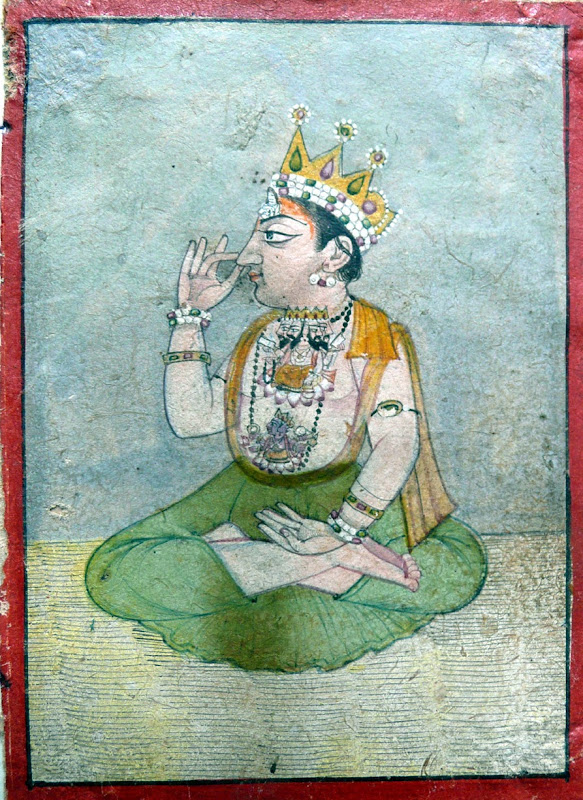
\includegraphics[width=1\textwidth]{pics/royalyogi2.jpg}
	\caption{A prince in royal gear performing breath-control (\textit{prāṇāyāma}).}
	\label{fig:royalyogi2}
\end{figure}

The second painting (Figure \ref{fig:royalyogi1}) from 1690-1700 C.E. depicts a crowned prince named Mandhāta seated in a yogic position and, as Hargreaves suggests, probably practising \textit{prāṇāyāma}. This picture contains the same three deities, just in another order. Here, the lower two are reversed, with Viṣṇu at the heart and Brahmā at the navel. The picture was obtained in India, Pahari, Nurpur and is currently in the Cleveland Museum of Art.

\begin{figure}[ht]
	\centering
  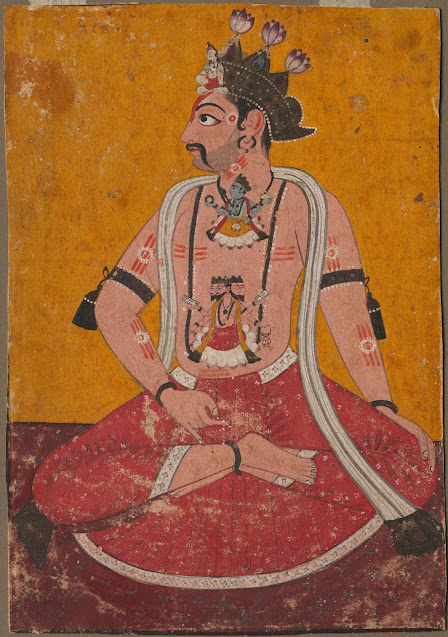
\includegraphics[width=0.7\textwidth]{pics/royalyogi1.jpg}
	\caption{The crowned prince Mandhāta seated in a yogic position.}
	\label{fig:royalyogi1}
\end{figure}

The third painting (Figure \ref{fig:royalyogi3}) is a miniature from circa the 19th century held in the Wellcome Collection. The painting illustrates a person called Appu Sahib Patumkar performing a yogic posture called \textit{dhanurāsana} ``bow-posture'' on an antelope's skin. According to Hargreaves, the practitioner's name suggests he is a person of a noble family.

\begin{landscape}
\begin{figure}[ht]
	\centering
  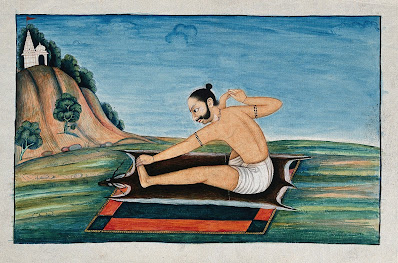
\includegraphics[width=1.3\textwidth]{pics/royalyogi3.jpg}
	\caption{Appu Sahib Patumkar performing jogh [\textit{āsana}].}
	\label{fig:royalyogi3}
\end{figure}
\end{landscape}

\newpage 
\section{Editorial matters}

\lettrine[lines=2, lhang=0.2, loversize=0.25]{T}{he} section ``Editorial Matters'' covers essential text-critical formalities. Following a description of the consulted and yet-to-be-consulted witnesses, there is an initial discussion of the title. That is particularly relevant in the case of Rāmacandra's text, where an unusual scenario arises: the text is known by more than six different titles according to colophons, title pages, library cards, the printed edition, and citations. That phenomenon requires further discussion. Subsequently, the source texts, testimonies and parallels are briefly described and contextualized. Next, I will present a stemmatic analysis, a presentation of the text's stylistic peculiarities, and an outline of the conventions used in the critical edition.

\subsection{Description of the consulted witnesses}
\vspace{0.25cm}
\begin{description}
\item[\textbf{Siglum:}] \Huge{\getsiglum{N1}} \nocite{ytbn1}
\item[\textbf{Catalogue:}] National Archives Kathmandu; microfilmed by the Nepalese German Manuscript Preservation Project (NGMPP) and catalogued by the Nepalese German Manuscript Cataloguing Project (NPMCP). 
\item[\textbf{Title:}] \emph{Tattvayogabindu} 
\item[\textbf{Ms. No.:}] B 38/31
\item[\textbf{Acc No.:}] NAK 5/2724
\item[\textbf{Dimensions:}] 26.5 x 8.5 cm x 13 folios 
\item[\textbf{Material:}] Paper
\item[\textbf{Language:}] Sanskrit
\item[\textbf{Script:}] Pracalita (Nepalākṣara)
\item[\textbf{Date:}] Nepal saṃvat 837 = 1716 CE
\item[\textbf{Condition:}] Incomplete (4 folios are missing)
\item[\textbf{Remarks:}] For now, this is the oldest dated surviving textual witness and often provides the best readings. After section \uproman{34}, there is a \textit{lacuna} until section \uproman{48}, approximately 23.50\% of the entire text is missing. 
\item[\textbf{Opening:}] \textit{śrīgaṇeśāya namaḥ} || \textit{śrī gurave namaḥ} || \textit{atha rājayogaprakāro  likhyate} ||
\item[\textbf{Final Colophon:}] \textit{iti śrī paramarahasyāṃ śrīrāmacaṃdraviracitāyāṃ tatvayogabiṃdu samāptaḥ} ||
\item[\textbf{Comments after Final Colophon:}] || \textit{śrī svasti} || || \textit{saṃvat 837} || \textit{vinā guru na siddhati} || \textbf{[Second hand adds in a mix of Nepālī and Newārī:]} \textit{eka vacana sosyā sālikaseṃ caudha bhuvana kā mola} || \textit{kahane soka haḍiyā avakyā vajāye ṃe ḍhola} || 1 || \textit{popoṣṭakaṃmā 10} | \textit{11} | \textit{12} | \textit{13} \textit{ja(m)mā 4 patra aghaḍiṣī ṭaṭāye .. ho} 
\end{description}
\newpage
\begin{description}
\item[\textbf{Siglum:}] \Huge{\getsiglum{N2}} \nocite{ytbn2}
\item[\textbf{Collection:}] National Archives Kathmandu; microfilmed by the Nepalese German Manuscript Preservation Project (NGMPP) and catalogued by the Nepalese German Manuscript Cataloguing Project (NPMCP).
\item[\textbf{Title:}] \emph{Tattvayogabindu} (The title folio reads: \textit{srī rājayogabinduprārambhaḥ}. The library card reads \textit{Rājayogatattvabindu}.)
\item[\textbf{Ms. No.:}] B 38/35
\item[\textbf{Acc No.:}] NAK 3/750
\item[\textbf{Dimensions:}] 33 x 16 cm x 11 folios   
\item[\textbf{Material:}] Paper \hspace{0.5cm} \textbf{Language:} Sanskrit \hspace{0.5cm} \textbf{Script:} Devanāgarī 
\item[\textbf{Date:}] not dated
\item[\textbf{Condition:}] Incomplete
\item[\textbf{Remarks:}] Manuscript \getsiglum{N2} has a \textit{lacuna} after section \uproman{34} up until section \uproman{48}. Approximately 23,50\% of the entire text is missing. The \textit{lacuna} is indicated on f.8 recto l.1. It stops at the same place where manuscript \getsiglum{N1} has missing folios. Thus, we have to assume that manuscript \getsiglum{N2} is a direct copy of manuscript \getsiglum{N1}. I decided to collate \getsiglum{N2} since it sometimes includes several different and sometimes better readings, which must be emendations and conjectures by the scribe. NGMCP catalogues another scan of the same manuscript under Ms. No. A 1327-14. However, the scan is poor.    
\item[\textbf{Opening:}] \textit{śrīgaṇeśāya namaḥ} || \textit{atha rājayogaprakāro  likhyate} ||
\item[\textbf{Final Colophon:}] \textit{iti śrī paramarahasye śrīrāmacaṃdraviracitāyāṃ tatvayogabindu samāptam} || 
\item[\textbf{Comments after Final Colophon:}] || \textit{śubham} || \textit{yad akṣarapadabhraṣṭaṃ mātrāhīnaṃ cayad bhavet} || \textit{tat sarvaṃ kṣamya tām eva prasīdaparameśvara} ||1|| \textit{sūrye turaṅge navacandraghasre jyeṣṭhākhyakṛṣṇe bhṛguvārayuktam} || \textit{tattvaprayogaḥ ṣaḍaharṣasaṃjñaṃ likhitaṃ suhetoḥ bhavatīha dehi} || \textit{bhūyāt} ||
\end{description}
\newpage
\begin{description}
\item[\textbf{Siglum:}] \Huge{\getsiglum{D}} \nocite{ytbd}
\item[\textbf{Collection:}] Indhira Gandhi National Centre for the Arts (IGNCA), cf. \citetitle{kaivalyadamanuscripts2005} of the Kaivalyadhama S.M.Y.M. Samiti (2005: 104-105). 
\item[\textbf{Title:}] \emph{Tattvayogabindu} 
\item[\textbf{Ms. No.:}] 30019
\item[\textbf{Dimensions:}] 21 x 10,3 cm x 16 folios   
\item[\textbf{Material:}] Paper
\item[\textbf{Language:}] Sanskrit
\item[\textbf{Script:}] Devanāgarī
\item[\textbf{Date:}] Vikram saṃvat 1841 = 1784 CE
\item[\textbf{Condition:}] Incomplete
\item[\textbf{Remarks:}] Folios 15 \& 16 are missing. The \textit{lacuna} of \getsiglum{D} strechtes from verse \uproman{44}.9 up to section \uproman{50}. The scan indicates that folio 19 is missing, too. However, the text is complete on folio 18.
\item[\textbf{Opening:}] \textit{śrīgaṇeśāya namaḥ} || \textit{śrī sarasvatyai namaḥ} || \textit{śrī nirañjanāya namaḥ} || \textit{atha rājayogaprakāro likhyate} || 
\item[\textbf{Final Colophon:}] \textit{iti paramahaṃsyāṃ śrī rāmacaṃdraviracitāyāṃ tatvayogabiṃdu samāptaḥ} || 
\item[\textbf{Comments after Final Colophon:}] \textit{śubham astu} | \textit{saṃvat 1841} || \textit{bhādau śudha 15 lī 0 ve sarva śake rā rāma rāma cha}
\end{description}
\newpage
\begin{description}
\item[\textbf{Siglum:}] \Huge{\getsiglum{U1}} \nocite{ytbu1}
\item[\textbf{Collection:}] Scindia Oriental Research Institute (SORI) Vikram University (Ujjain), cf. \citetitle{kaivalyadamanuscripts2005} of the Kaivalyadhama S.M.Y.M. Samiti (2005: 104-105, 246-247). 
\item[\textbf{Title:}] \emph{Tattvayogaviduḥ} (The title folio reads: \textit{atha yogataprāraṃbhaḥ}.)
\item[\textbf{Ms. No.:}] 1574
\item[\textbf{Dimensions:}] 20 x 13 cm x 45 folios   
\item[\textbf{Material:}] Paper
\item[\textbf{Language:}] Sanskrit
\item[\textbf{Script:}] Devanāgarī
\item[\textbf{Date:}] not dated 
\item[\textbf{Condition:}] Incomplete
\item[\textbf{Remarks:}] Manuscript \getsiglum{U1} contains a \textit{lacuna} within section \uproman{57}. This comparatively large and important section is almost entirely absent in this manuscript. Especially during the great \textit{lacuna} in \getsiglum{N1} and \getsiglum{N2}, the readings of this manuscript became important for the constitution of the text.     
\item[\textbf{Opening:}] \textit{śrīgaṇeśāya namaḥ} || \textit{atha rājayoga likhyate} ||     
\item[\textbf{Final Colophon:}] \textit{iti śrī pāramahaṃsyāṃ śrī rāmacaṃdraviracitāyāṃ tatvayogaviduḥ samāptaḥ} 
\item[\textbf{Comments after Final Colophon:}] \textit{śubhaṃ bhūyāt} ||
\end{description}
\newpage
\begin{description}
\item[\textbf{Siglum:}] \Huge{\getsiglum{U2}} \nocite{ytbu2}
\item[\textbf{Collection:}] Scindia Oriental Research Institute (SORI) Vikram University (Ujjain), cf. \citetitle{kaivalyadamanuscripts2005} of the Kaivalyadhama S.M.Y.M. Samiti (2005: 394-395), here catalogued under the title \emph{Rājayoga}. 
\item[\textbf{Title:}] \emph{Tattvabinduyoga}. (The title folio reads: \textit{atha śrī rājayogaprāraṃbhaḥ} || \textit{śrīrāmavaracitena} ||)
\item[\textbf{Ms. No.:}] 6082
\item[\textbf{Dimensions:}] 21 x 11 cm x 37 folios   
\item[\textbf{Material:}] Paper \hspace{0.5cm}  \textbf{Language:} Sanskrit \hspace{0.5cm} \textbf{Script:} Devanāgarī
\item[\textbf{Scribe:}] Bābājī Rājadherakara   
\item[\textbf{Date:}] Śaka 1805, Vikram saṃvat 1940 = 1883 CE
\item[\textbf{Condition:}] Complete
\item[\textbf{Remarks:}] This manuscript contains additional information on the ninefold \textit{cakra} system in the sections \uproman{4}-\uproman{12}.       
\item[\textbf{Opening:}] \textit{śrīgaṇeśāya namaḥ} || \textit{śrī gurave namaḥ} || \textit{atha rājayogaprakāro likhyate} ||
\item[\textbf{Final Colophon:}] \textit{iti śrī rāmacaṃdraparamahaṃsaviracitas tatvabiṃduyogasamāptaḥ} ||
\item[\textbf{Comments after Final Colophon:}]  \textit{śrī śubhaṃ bhavatu} ||  \textit{śrīsītārāmārpaṇam astuḥ} ||  \textit{idaṃ pustakaṃ} ||  \textit{śake 1805} ||  \textit{vikramārka saṃmat} ||  \textit{1940} || \textit{jayanām asaṃvatsare} ||  \textit{udagayaṇe} ||  \textit{griṣmaṛtau}? ||  \textit{vaiśākhe māse} ||  \textit{kṛṣṇapakṣe} ||  \textit{tithau 23} ||  \textit{bhānuvāsare} ||  \textit{prathamayāmye} ||  \textit{śrīkṣetra avaṃtikāyāṃ} ||  \textit{śrī mahārudramahākālasaṃnidhāne na saṃpūrṇaṃ} ||  \textit{lekhanaṃ ānaṃt? suta? bābājī rājadherakareṇa likhyate} ||  \textit{yādṛśaṃ pustakaṃ dṛṣtvā tādṛsaṃ likhitaṃ mayā} ||  \textit{yadi śuddhaṃ aśuddho vā mama doṣo na dīyate} ||1|| \textit{śrīrāma} || cha ||
\end{description}
\newpage
\begin{description}
\item[\textbf{Siglum:}] \Huge{\getsiglum{B}} \nocite{ytbb}
\item[\textbf{Collection:}] Oxford Bodleian Library (OBL), Sanskrit Manuscripts of Candra Shum Shere (CSS), cf. \citetitle{kaivalyadamanuscripts2005} of the Kaivalyadhama S.M.Y.M. Samiti (2005: 102-103). 
\item[\textbf{Title:}] The title folio reads: \textit{tatvabiṃduyogaḥ}. 
\item[\textbf{Ms. No.:}] d. 458 (7) 
\item[\textbf{Dimensions:}] 15 folios 
\item[\textbf{Material:}] Paper
\item[\textbf{Language:}] Sanskrit
\item[\textbf{Script:}] Devanāgarī
\item[\textbf{Date:}] not dated
\item[\textbf{Condition:}] Incomplete
\item[\textbf{Remarks:}] First and last folio missing. Evidence of \getsiglum{B} starts at section \uproman{9}. This is one of the manuscripts donated by Shum Shere, Chandra Mahārāja Chandra Shamsher Jang Bahadur Rana in 1909. 
\item[\textbf{Opening:}] not available 
\item[\textbf{Final Colophon:}] not available 
\item[\textbf{Comments after Final Colophon:}] not available
\end{description}
\newpage
\begin{description}
\item[\textbf{Siglum:}] \Huge{\getsiglum{L}} \nocite{ytbl}
\item[\textbf{Collection:}] Lalchand Research Library Ancient Indian Manuscript Collection; \citetitle{srivastava2017lal} (2017: 251) = Hoshiarpur Vishveshvarananda Vedic Research Institute's (HVVRI) Ms. No. 5876 ``\emph{Tattvabindūyogaḥ} by Rāmacandra'', cf. \citetitle{kaivalyadamanuscripts2005} of the Kaivalyadhama S.M.Y.M. Samiti (2005: 102-103). All Manuscripts of HVVRI have been transferred to Chandigarh. 
\item[\textbf{Title:}] \emph{Tattvabinduyoga} 
\item[\textbf{Ms. No.:}] 5876
\item[\textbf{Dimensions:}] ?? x ?? cm x 43 folios 
\item[\textbf{Material:}] Paper
\item[\textbf{Language:}] Sanskrit
\item[\textbf{Script:}] Devanāgarī
\item[\textbf{Date:}] not dated
\item[\textbf{Condition:}] Complete 
\item[\textbf{Remarks:}] The manuscript is digitized and available online under \url{https://dav.splrarebooks.com/collection/view/tattvabinduyogah}
\item[\textbf{Opening:}] \textit{śrīgaṇeśāya namaḥ} | \textit{atha tattvabiṃduyogaprāraṃbhaḥ}
\item[\textbf{Final Colophon:}] \textit{iti rājamacaṃdraparahaṃsa viracites tatvabiṃduyogasamāptaṃ} || \textit{śrī kṛṣṇārpaṇam astu} || \textit{cha} ||
\item[\textbf{Comments after Final Colophon:}] not available  
\end{description}
\newpage
\begin{description}
\item[\textbf{Siglum:}] \Huge{\getsiglum{P}} \nocite{ytbp}
\item[\textbf{Collection:}] Bhandakar Oriental Research Institute (BORI), cf. \citetitle{kaivalyadamanuscripts2005} of the Kaivalyadhama S.M.Y.M. Samiti (2005: 394-395), here catalogued under the title \emph{Rājayoga}. 
\item[\textbf{Title:}] \emph{Tattvabinduyoga}. The library card reads \textit{Rājayoga} (\textit{Tattvabinduyoga}).  
\item[\textbf{Ms. No.:}] 644
\item[\textbf{Dimensions:}] 25 x 11,2 cm x 29 folios
\item[\textbf{Material:}] Paper 
\item[\textbf{Language:}] Sanskrit
\item[\textbf{Script:}] Devanāgarī
\item[\textbf{Date:}] Vikram saṃvat 1867 = 1810 CE
\item[\textbf{Condition:}] Complete
\item[\textbf{Remarks:}] 
\item[\textbf{Opening:}] \textit{śrīṇe ya maḥ} | \textit{atha rājayoga liṣyate}
\item[\textbf{Final Colophon:}] \textit{iti śrīrāmacaṃdraparamahaṃsa viracitas tatvabinduyogasamāptaḥ}
\item[\textbf{Comments after Final Colophon:}] \textit{saṃvat 1867 pauṣakṛṣṇaḥ 12 ravau śubham bhuyāt} || \textit{cha} || 
\end{description}
\newpage
\begin{description}
\item[\textbf{Siglum:}] \Huge{\getsiglum{E}} \nocite{ytbe}
\item[\textbf{Title:}] \emph{Binduyogaḥ with Bhāṣaṭīkā}
\item[\textbf{Collection:}] Kaivalyadhama Library
\item[\textbf{No.:}] 6387
\item[\textbf{Editors:}] Jvālāprasāda Miśra, son of the revered scholar Sukhānanda Miśra
\item[\textbf{Material:}] Paper
\item[\textbf{Language:}] Sanskrit and Hindi
\item[\textbf{Script:}] Devanāgarī
\item[\textbf{Date:}] 1905 CE
\item[\textbf{Condition:}] Contains \textit{lacuna}, Large section is transposed. Problematic passages of the unknown exemplar were emended or conjectured by the Pandit.  
\item[\textbf{Remarks:}] Printed Edition written in Mumbai together with Hindi Translation and \emph{Bhāṣaṭīkā} commentary. 
\item[\textbf{Opening:}] \textit{śrīgaṇeśāya namaḥ} | \textit{rājayogāntargataḥ} || \textit{binduyogaḥ} 
\item[\textbf{Final Colophon:}] \textit{iti rājayoge candraparamahaṃsaparipūrṇapīṭhamāhātmyaprakāśakaḥ binduyogaḥ samāptaḥ} || \textit{śubham astu} ||  
\item[\textbf{Comments after Final Colophon:}] \textit{iti śrīsarvaguṇasampannapaṃḍitasukhānandamiśrasūrisūnupaṇḍitajvālāprasādamiśrakṛtabhāṣāṭīkāsahito rājayoge binduyogaḥ samāptaḥ} || \textit{śubham astu} || \textit{śrīr astu} ||
\end{description}
\newpage

\subsection{Manuscripts not consulted}

The official commencement of the funded period of this dissertation project on 15 March 2021 coincided with the numerous lockdowns and travel restrictions imposed due to the COVID-19 pandemic. Consequently, during the phase of the dissertation when additional manuscripts could have been collected, I was confined to my desk at home. The brief windows of opportunity for travel were further obstructed by pandemic-related familial complications. Although I have identified the following manuscripts in catalogues, I have regrettably been unable to consult them for this work thus far.

Update: Only a few weeks before the submission of this dissertation, I was able to locate additional manuscripts of this text in catalogues, listed under the title \textit{Rājayogaprakāra} in the NCC, which is why I had previously overlooked them. According to current knowledge, a total of seven manuscripts from the listed ones should be obtainable, and their consultation would be desirable. One of the seven is particularly promising, as it must belong to the \alpha-group, while four of them, judging by their title, belong to the \beta-group. Two of the manuscripts bear the title \textit{Rājayogaprakāra} and are yet to be classified. Another manuscript titled \textit{Rājayogaprakā} is reported in the catalogue to be extremely damaged, incomplete (only two folios remain), and quite recent. The whereabouts of two other catalogued manuscripts cannot be precisely determined at present. I will consult these manuscripts and, if necessary, incorporate them into the final printed version of this work for publication. 

\subsubsection{Important}

\begin{itemize}
\item Kolkata (former Calcutta) Sanskrit Library. NCC: CS. III. 65. = \citetitle[1900: 37]{calcutta1900}. Title: \emph{Tattvayogabinduḥ}. Author: Paramahaṃsa Rāmacandra. Material: Countrymade white paper. Dimensions 9x 3 inches x 22 folios. Date: Vikram Saṃvat 1847 (1790 CE). Condition: old, slightly worm-eaten, generally correct and complete. This manuscript is the most important among the unconsulted ones. The title indicates that it belongs to the \alpha-group. 
\item Royal Asiatic Society of Bengal (RASB). Kolkata. \nocite{newcataloguscatalogorum8} \nocite{newcataloguscatalogorum23} \citeauthor{hall1859} (1859: 14) reports a manuscript \uproman{25} in his catalogue called ``Tattva-bindu-yoga''. The entry says, ``Defining the divisions of Yoga. By Ramachandra Paramahansa. Leaves 18, \textit{śloka}s 440. F.E.H.''. The amount of \textit{śloka}s must approximate the amount of text and not the actual number of verses since the text mixes prose and verse but is mainly written in prose. The abbreviation ``F. E. H.'' indicates that this manuscript personally belonged to Fitzedward \citeauthor{hall1859}. The New Catalogus Catalogorum (NCC) (Vol. 8: 54) revealed: ``Tattvabindu(yoga) - by Rāmacandra Paramahamsa. Ben. 66. IM. 5441 (inc.). Hall p. 14.''. The abbreviation ``IM'' indicates that the manuscript of \citeauthor{hall1859} should be deposited at the Royal Asiatic Society of Bengal (RASB). NCC (Vol. 23: 259) lists two manuscripts at the RASB: VIII. B. 6605. 6606. One of them should be the \citeauthor{hall1859} manuscript. The title of the manuscript indicates that it should belong to the \beta-group. 
\item Sanskrit Vidyāpeetham near Yamuna Kinare, Etawah (U.P). Title: \textit{Tattvabindūyogaḥ}. Author: Rāmacandraḥ. Script: Devanāgarī. Condition: incomplete. Ms. No: ESV 7 (P20), cf. \citetitle{kaivalyadamanuscripts2005} of the Kaivalyadhama S.M.Y.M. Samiti (2005: 102-103). The title of the manuscript indicates that it should belong to the \beta-group. 
\item  Nagpur University Library (NUL). \citetitle[1957:]{nagpur1957}. Ms. No. 6769. Title: \emph{Tattvabindūyogaḥ}. Author: Rāmacandra Paramahaṃsa. Material: Paper. Script: Devanāgarī. Judging by the title, this manuscript belongs to the \beta-group. 
\item Ānandāśrama Pune. Title: \emph{Rājayogaprakāra}. Ms. No.: 2872. Website: \url{https://www.aanandashram-sanstha.org/}
\item Baroda Oriental Institute. NCC (Vol. 23: 259) reports a manuscript in ``Baroda II. 10558''. This is \citetitle{baroda1950} (1950: 1238) reports it under the title \textit{Rājayogaprakāraḥ}. I was able to obtain the manuscript two weeks before submission of the dissertation. I would like to thank Harshal Bhatt for his immediate help. The title in the colophon is \emph{Rājayogavicāra}. The manuscript decends directly from the \alpha-group. It was written by a learned scribe since the manuscript contains creative solutions for the problematic passages. A few readings appear to be helpful and confirm some emendations. Thus, it will be collated for publication. However, a first reading of this manuscript suggests that it will not improve the text significantly. %%Harshal! 
\end{itemize}
  
\subsubsection{Damaged}
\begin{itemize}
\item Lucknow Sanskrit Parishad. \citetitle[2021: 224]{lucknow2021}. Title: \emph{Rājayoga Prakāraḥ?}. Author: Rāmacandra. Serial No.: 74. Accession No.: 1266. Condition: Incomplete. Only two folios. Condition and Age: Recent. 
\end{itemize}

\subsubsection{Probably unobtainable}
\begin{itemize}  
\item NCC: Darbhanga Raj 2146 (inc.). Probably: Descriptive Catalogue of Raj Manuscripts Preserved in Kameshwar Singh Sanskrit University, Darbhanga. Title=\emph{Rājayogaprakāra}. \url{https://lnmu.ac.in}. Unfortunately, I have no access to the catalogue.
\item CPB. (Ms. No.: 4579-80. \citetitle[1926: 408]{nagpur1926} (1926: 408). Title ``Rājayoga''. Author: Rāmacandra Paramahaṃsa. Subject: Yoga. Owner. (4579) Nārāyaṃ Purānī of Hardā (Hoshangābād district). (4580) Viśvambharnāth of Ratanpur (Bilāspur district). Comment: According to what I heard from my colleagues, these manuscripts might be hard to track down. Possibly, one of them ended up in the above-mentioned collection of the Nagpur University Library (NUL). 
\end{itemize}
  
\subsection{Discussion of the text's original title}
\label{titlediscussion}
It is striking that there is disagreement among the witnesses of Rāmacandra's text regarding the title. The variants are: \emph{Tattvabinduyoga}, \emph{Tattvayogabindu}, \emph{Tattvayogaviduḥ}, \emph{Rājayogatattvabindu}, \emph{Binduyoga}, \emph{Rājayoga}, \emph{Rājayogaprakāra}, \emph{Rājayogavicāra} and \emph{Tattvajñānapradīpikā}. Four of the manuscripts of the \beta-group\footnote{See p. \pageref{stemma} for the stemmatic analysis of the manuscripts.} consulted in this critical edition—\getsiglum{B}, \getsiglum{L}, \getsiglum{P}, \getsiglum{U2}, and three additional yet unexamined manuscripts likely belonging to the \beta-group—bear the title \emph{Tattvabinduyoga} according to their colophons or cover pages. The printed edition \getsiglum{E} is titled \emph{Binduyogaḥ}. From a stemmatological perspective, the printed edition \getsiglum{E} must descend from a \beta-group manuscript. 

It is challenging to derive a convincing meaning from the title \emph{Tattvabinduyoga} and even \emph{Binduyoga}, especially considering the actual content of the work. The term \textit{bindu} does not appear even once in the entire text. Exploring various possible interpretations and translations of this compound, such as ``Yoga of the points [of reality],'' none seem satisfactory. If an interpretation of such a title were correct, one would expect an explanation of \textit{bindu} in the text. Although various yoga practices involving concentration on specific bodily points are mentioned frequently, these are never referred to as \textit{bindu}s.

It is not apparent why Jvālāprasāda Miśra, the editor of the 1905 printed edition, made the editorial decision to discard the title of his exemplar and rename the text to \emph{Binduyoga} as it does not enhance the title's relevance to the work. The term \textit{binduyoga}, for example appearing in the \emph{Amṛtasiddi} (7.14), where \textit{binduyoga} designates its core yoga practice\footnote{\emph{Amṛtasiddi} 7.14: \textit{binduyogaṃ parityajya yo mohād anyam icchati} | \textit{sa śākhoṭakavṛkṣeṣu mūḍho jāgarti niṣphalam} ||} is not applicable here, as Rāmacandra neither teaches \textit{mudrā}s nor practices involving sexual fluids.\footnote{On the contrary, Rāmacandra discredits the practice of \textit{mudrā}s in section \uproman{58}.} Nor does \textit{bindu} function as an ultimate \textit{tattva} within the 36-\textit{tattva} systems of Śaivism, since such a \textit{bindu} is not mentioned by Rāmacandra.\footnote{See \citeauthor[1996: 177]{gengnagel1996} for the 36 \textit{tattva}s of Śaivasiddhānta. Additionally, see \citeauthor[2016: 77 et seqq.]{goodall2016tattvas} for a discussion on the genesis of the Śaiva \textit{tattva} systems.} On the contrary, Rāmacandra's text teaches a tenfold \textit{tattva} system,\footnote{\emph{Yogatattvabindu} \uproman{22} l.4 mentions Earth (\textit{pṛthvī}), Water (\textit{āpa}), Fire (\textit{tejas}), Wind (\textit{vāyu}), Space (\textit{ākāśa}), Mind (\textit{manas}), Intellect (\textit{buddhi}), Illusion (\textit{māyā}), Transformations (\textit{vikāra}), and Form (\textit{rūpa}).} The only plausible, simple, and natural explanation is that Jvālāprasāda Miśra must have understood \emph{Binduyoga} as ``Yoga of the points [for concentration],'' given that larger chunks of the text teach \textit{cakra}s, \textit{lakṣya}s, and \textit{ādhāra}s for meditation. For these reasons, and notably because the term \textit{bindu} does not appear in the work, it is highly unlikely that Rāmacandra's text was originally titled \emph{Tattvabinduyoga}.

Instead, the title of the \beta-group manuscripts likely originated from the same archetype as the \alpha-group manuscripts, specifically \getsiglum{D}, \getsiglum{N1}, \getsiglum{N2}, \getsiglum{U1}, and an as-yet unexamined manuscript, all of which bear the title \emph{Tattvayogabindu} in their colophons. Given that the \alpha-group not only contains the oldest dated manuscript of the text but also frequently offers superior readings, it can be asserted with high confidence that the \beta-group title resulted from a metathesis of the two compound elements \textit{bindu} and \textit{yoga}.

Considering the aforementioned issues with the term \textit{bindu}, which appears only in the title and not within the text, this title makes a bit more sense. The term \textit{°bindu} is a common suffix in titles of various Sanskrit texts.\footnote{See, for example, \citetitle{stb1}\nocite{stb2} NGMPP, Ms. No. MA 905-3 and NGMPP, Ms. No. E 1189-13 (``Drops of the [supreme] reality of Siddhānta''); \emph{Nyāyabindu} (``Drops of reasoning''), cf. \nocite{newcataloguscatalogorum10} NCC Vol 10. (2007: 252); \emph{Nirṇayabindu} (``Drops of verdict''), NCC Vol 10. (2007: 146); \emph{Bhaktibindu} (``Drops of devotion''), NCC Vol 15. (2007: 148); \emph{Dharmabindu} (``Drops of law''), NCC Vol. 9 (2007: 257), etc.\nocite{newcataloguscatalogorum9}\nocite{newcataloguscatalogorum15}} The employment of the term ``\textit{°bindu}'' in the titles of these texts emphasises the idea of expressing essential, seminal points in a condensed way to make complex topics more accessible and intelligible. As such, the term suggests that each work strives to distil the essence of its subject into basic doctrines or principles. In the case of Rāmacandra's text, \textit{°bindu} makes perfect sense when understood in this way.     

However, this title still leaves some doubts. Although the first part of the compound now makes sense, the remaining parts do not fit well. \emph{Tattvayogabindu} could be interpreted as ``Drops of the yoga of reality'' or ``Drops of the yoga of principles,'' but this again does not align with the text's content. Evidence suggesting that other recipients did not accept the titles of the \alpha- and \beta-groups appears in Sundaradeva's \emph{Haṭhasaṅketacandrikā}, which cites extensively from Rāmacandra's text\footnote{For references see p.\pageref{hathacandrika}.} but does so without citation, which is unusual since he typically references his sources. Another testimony, titled \emph{Yogasaṃgraha}, cites approximately 20\% of Rāmacandra's entire text.\footnote{For references see p.\pageref{yogasamgraha}.} Here, the author in his quotation renames the text to \emph{Tattvajñānapradīpikā}. Other titles also circulate, found both on manuscript cover pages and in manuscript catalogues. These titles, like \emph{Rājayoga}, \emph{Rājayogaprakāra}, or \emph{Rājayogavicāra} attempt to capture the work's content better and may have been lent because the title available to them in the colophons appeared misleading. 

How can this be explained? Is it possible that even the title of the \alpha-group has succumbed to textual corruption? Could it be that the title of the \alpha-group is also a result of metathesis and that the three components of the title were confused by scribes early in the transmission? The following text-imminent observation supports the possibility that no surviving manuscript preserves the title in its original form. In section \uproman{58}, ll. 1-8 Rāmacandra's text reads:

\begin{quote}
  \label{mahatmya}
  \textit{idānīṃ yogasya māhātmyaṃ kathyate} |
  \textit{guroranugrahāt} | \textit{śāstrasya paṭhanāt} | \textit{ācārakaraṇāt} | \textit{vedāntarahasya śravaṇāt} |
  \textit{dhyānakaraṇāt} | \textit{layasādhanāt} | \textit{upavāsakaraṇāt} | \textit{caturaśītyāsanasādhanāt} | \textit{vairāgyasyotpatteḥ} | \textit{vairāgyakaraṇāt} | \textit{haṭhayogasya karaṇāt} | \textit{iḍāpiṅgalayoḥ pavanadhāraṇāt} | \textit{mahāmudrādidaśamudrāsādhanāt} | \textit{maunakaraṇāt} | \textit{vanavāsāt} | \textit{bahutarakleśakaraṇāt} | \textit{bahutarakālaṃ} \textit{yantramantrādisādhanāt} | \textit{tapaḥkaraṇāt} | \textit{bahutarārthādānāt} | \textit{tīrthasevākaraṇāt} | \textit{āśramācārapālanāt} | \textit{saṃnyāsagrahaṇāt} | \textit{ṣaḍdarśanagrahaṇāt} | \textit{siromaṇḍanāt} | \textit{anyopāyakaraṇāt} | \textit{\textbf{yogatattvaṃ} na prāpyate} | \textit{sa tu yogo gurusevayā prāpyate} |
\end{quote}

\begin{quote}
Now, the majesty of yoga is taught.\\ As a result of the grace of the teacher, studying the teaching, execution of good conduct, hearing the secret of Vedānta, meditation, dissolution, fasting, practising 84 postures, generating indifference, cultivating indifference, doing Haṭhayoga, holding the breath of the Iḍā- and Piṅgalā-channels, practising the ten seals [like] the great-seal etc., observing silence, dwelling in the forest, causing excessive distress, practising Mantra and Yantra, etc. for a long time, doing austerities, giving many donations, frequenting places of pilgrimage, preserving the custom of the stages of life, adhering renunciation, grasping the six philosophies, shaving the head, doing other methods, the \textbf{reality of yoga} is not attained. It [the reality of yoga] is truly attained by serving the teacher.
  \end{quote}

  The negation of these practices, associated with yoga and even those previously taught by Rāmacandra himself, clearly illustrates that this passage forms a climax of the entire text. The word combination \textit{tattvayoga} is never found throughout the text, whereas \textit{yogatattva} appears only in this singular location. Given the centrality of this passage and the previously noted inconsistencies in the titles from the \alpha- and \beta-groups, it seems most likely that the work's original title was \emph{Yogatattvabindu}.
  
  \begin{figure}[h!]
    \centering
    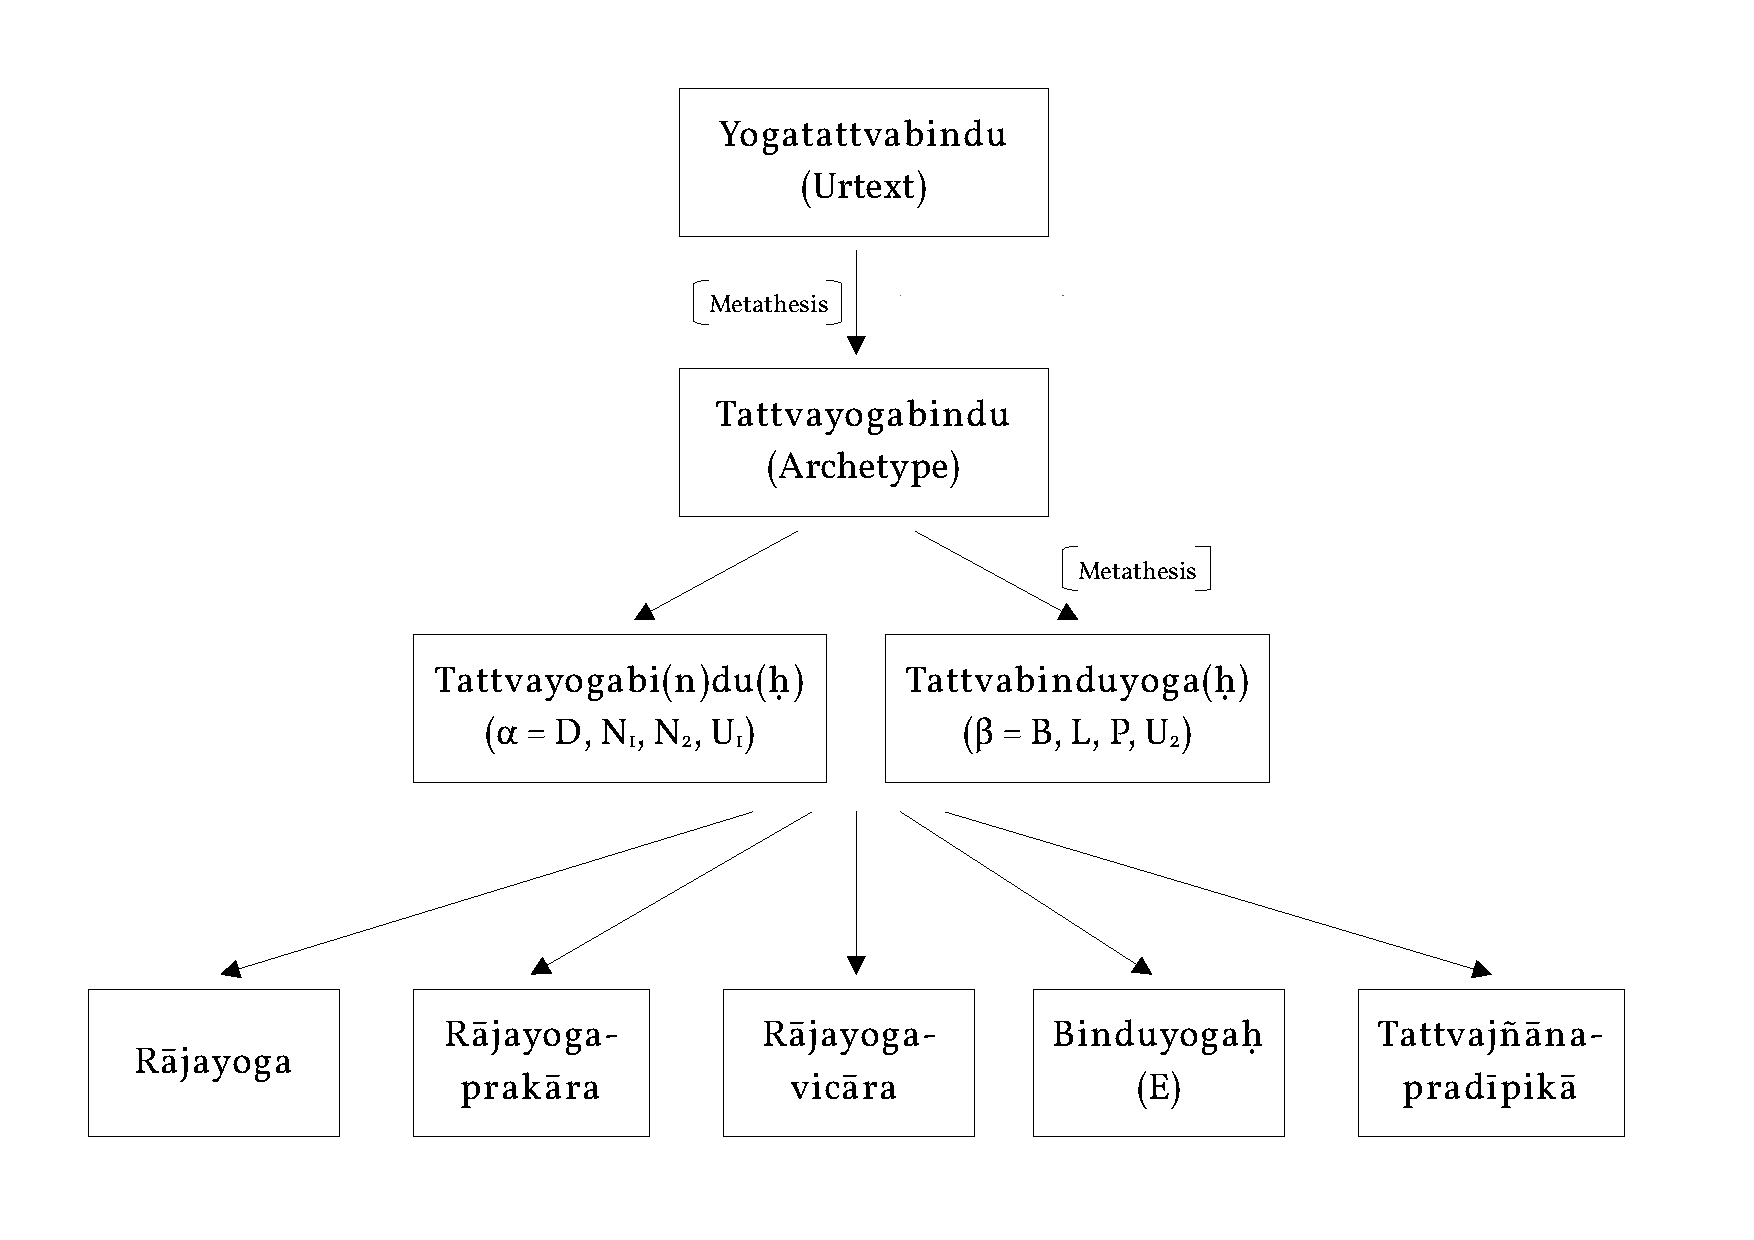
\includegraphics[width=1\textwidth]{pics/titel-hypothese.pdf} % Passe die Breite nach Bedarf an
    \caption{The hypothesis of transmission of the \emph{Yogatattvabindu}'s title.}
    \label{fig:titel-hypothese}
\end{figure}

Considering the overall content of the text, the title \textit{Yogatattvabindu}, which can be translated as ``Drops of the [supreme] reality of yoga,'' is convincing. Taking the \textit{bindu} as a plural even captures the great variety of yogas presented in the initial yoga taxonomy. Another argument for this emendation is the frequency of this word combination in common e-text collections. In 6569 searched texts, many within the yoga and Tantra genres, the combination \textit{tattvayoga} yields only 19 hits. None of these hits can be meaningfully applied to our text. In contrast, the combination \textit{yogatattva} appears 109 times with congruent meanings and is also frequently found in the titles of yoga works.\footnote{For example, \emph{Yogatattva}, cf. NCC Vol. 22 (2007: 70); \emph{Yogatattvasamāsasūtra}, cf. NCC Vol. 22 (2007: 70) \nocite{newcataloguscatalogorum22}; \emph{Yogatattvaupaniṣad}, cf. \citetitle{yogatattvopanishad} (Ed. p. 363-388); \emph{Yogatattvadīpikā}, cf. \citetitle{kaivalyadamanuscripts2005} (2005: 232); \emph{Yogatattvopaniṣaddīpikā}, cf. \citetitle{kaivalyadamanuscripts2005} (2005: 232), etc. Furthermore, the position of \emph{°tattva°} is also supported by its use in the title \emph{Haṭhatattvakaumudī} by Sundaradeva.} In favour, we note that manuscript \getsiglum{N2}'s library card reads \textit{Rājayogatattvabindu} and the title page of manuscript \getsiglum{U1} introduces the text with \textit{atha yogata[ttva?]prāraṃbhaḥ}. 

The existence of so many variants of the title in the colophons, cover pages of manuscripts, and catalogue entries can ultimately only be attributed to an early scribal error in the text's transmission—a metathesis of entire words, which early on transformed the compound of the work's title from \textit{yogatattva°} into \textit{tattvayoga°}. Subsequent scribes or editors either caused another metathesis, attempted to correct the inappropriate title, replaced it entirely, or omitted it altogether.

\subsection{Description of the sources}

In the critical edition of the \emph{Yogatattvabindu}, the author's sources are indicated in the first layer of the critical apparatus, corresponding to the respective passage. Overall, two texts form the basis of Rāmacandra's work: the \emph{Yogasvarodaya} and the \emph{Siddhasiddhāntapaddhati}. However, Rāmacandra does not provide references for these sources in any instance. On the one hand, there are some direct quotations, often in the form of verses. On the other hand, which constitutes the majority, Rāmacandra used his sources as a textual basis, either transforming them into prose, paraphrasing and editorially altering them or blending the contents of both sources. Nevertheless, the passages can be identified, as the contents of these sources are highly similar. It is so similar that glancing at the source texts helped make the correct editorial decisions or appropriately correct corrupt passages.

\subsubsection{Yogasvarodaya}
\label{svaro}
The \emph{Yogasvarodaya} (YSv) is the main source text, and Rāmacandra's \emph{Yogatattvabindu}. Rāmacandra derives most of his content from this text and even follows its structure to a great extent. The majority of sections in the \emph{Yogatattvabindu} result from Rāmacandra rewriting the \emph{śloka}s of the \emph{Yogasvarodaya} into prose, incorporating specific editorial changes to align with his agenda. Thus, this text is of utmost importance for the reconstruction of the \emph{Yogatattvabindu}'s doubtful passages. The text will be described in detail in the chapter ``Comparative analysis of the complex early modern yoga taxonomies''.\footnote{See p. \pageref{yogasvarodayadescription}.} Hence, another treatment would be redundant. So far, the \emph{Yogasvarodaya} is a text known solely through quotations found in the \emph{Prāṇatoṣiṇī} and \emph{Yogakaṇikā}, which will be described below. Manuscripts have yet to be found and remain a desideratum for the time being. 

\subsubsection{Prāṇatoṣiṇī}
\label{tosi}
The \textit{Prāṇatoṣiṇī} (PT) by Rāmatoṣaṇa\footnote{Although the printed editions identify Rāmatoṣaṇa as the author of this work, sometimes bearing the titles Vidyālaṃkāra or Bhaṭṭācārya, \citeauthor{shastri1905} (1905: 2) mentions another name: ``Babu Prāṇakṛṣṇa Visvās of Khaṛhadaha, within ten miles of Calcutta, collected in the beginning of the nineteenth century a large number of Tantra, Purāṇa and Smṛti MSS., for the purpose of compiling Prāṇatoṣiṇī, Prāṇakṛṣṇā Kriyāmbudhi and other encyclopaedic works on Hindu ritual and worship.''

Since the \textit{Prāṇatoṣiṇī} is frequently cited in recent secondary literature on tantric studies but lacks detailed studies, critical editions, or complete translations into Western languages, this discrepancy remains unresolved.} is a Tantra compendium (\textit{nibandha}) from the 19th century, compiled by the author in Bengal.\footnote{\cite{ramatosana}.} This extensive compendium addresses creation, the four \textit{puruṣārthas}, and devotion. The \textit{Prāṇatoṣiṇī} is divided into six major \textit{kāṇḍa}s (``sections''): 1. \textit{sargakāṇḍa} (subject: the creation of the universe and cosmogony), 2. \textit{dharmakhaṇḍa} (subject: rituals and Dharma of the twice-born), 3. \textit{arthakāṇḍa} (subject: daily routine, deity worship, purification practices, rites, offerings, etc.), 4. \textit{kāmyakāṇḍa} (subject: wish-fulfilment practices, protective mantras, etc.), 5. \textit{bhaktikāṇḍa} (subject: performance of devotional deity worship), and 6. \textit{jñānakāṇḍa} (subject: Mokṣa, yoga, etc.). The author draws from a multitude of texts circulating in this region during the 19th century.

Additional topics of the \textit{Prāṇatoṣiṇī} range from \textit{mantras}, \textit{yantras}, and their meanings\footnote{See \citeauthor[2010: 69-70]{slouber2010}.} to meditations, religious stories, legends, and deity worship,\footnote{See \citeauthor[1997: 149-150]{kinsley1997}.} the six acts of magic, tantric rituals including sexual rites, and various areas of tantric philosophy.\footnote{See \citeauthor[2010: 100]{urban2010}.}

The \textit{Prāṇatoṣiṇī} incorporates a total of 304 verses from the \textit{Yogasvarodaya} in its \textit{jñānakāṇḍa}.\footnote{\emph{Prāṇatoṣiṇī}, 1898: 831-848.} Therefore, it is currently the most extensive source of the \emph{Yogasvarodaya}. All its verses are cited with the reference \textit{yogasvarodaye}. These verses are quoted in a largely coherent sequence, giving the reader the impression of having the complete transmission of the text. However, this is not the case. Many additional verses of the \emph{Yogasvarodaya} can be found in the \emph{Yogakarṇikā} described below. There are numerous overlaps between the quotations. The main difference lies in the fact that, unlike the \textit{Prāṇatoṣiṇī}, the \emph{Yogakarṇikā} primarily includes practical instructions from the \textit{Yogasvarodaya}, such as instructions for \textit{prāṇāyāma}-, \textit{kumbhaka}-, or \textit{mudrā} techniques.

\subsubsection{Yogakarṇikā}
\label{karni}
The \emph{Yogakarṇikā} (YK) of Nāth Aghorānanda is another significant source of the \emph{Yogasvarodaya}.\footnote{\cite{yogakarnika}.} The \emph{Yogakarṇikā} is an extensive anthology on yoga, comprising 1552 verses divided into 15 \textit{pāda}s. The text derives its verses from a wide array of sources, often, though not always, citing them with references. Besides various Purāṇas (\emph{Mārkandeyapurāṇa}, \emph{Narasiṃhapurāṇa}, etc.) and Tantras (\textit{Kūbjikamatatantra}, \textit{Grahayāmala}, \emph{Rudrayāmala}, etc.), Nāth Aghorānanda also cites texts from the Haṭha and Rājayoga genres (\emph{Yogasvarodaya}, \emph{Haṭhapradīpikā}, \emph{Dattātreyayogaśāstra}, \emph{Gheraṇḍasaṃhitā}, \emph{Yogayājñavalkya}, various works attributed to Gorakṣa, etc.). Based on the established dating of the \emph{Yogasvarodaya}, which must have been written before 1659 CE,\footnote{Cf. p.\pageref{dating}.} and Mallinson's dating of the \emph{Gheraṇḍasaṃhitā} to circa 1700 CE,\footnote{\citeauthor[2004: xiv]{MallinsonGheranda}.} we can confidently assume that the \emph{Yogakarṇikā} was written no earlier than the 18th century.
The fifteen \textit{pāda}s are thematically structured as follows:

\begin{enumerate}
\item \textit{dinacārya} (``daily routine''); 280 verses
\item \textit{lakṣādiyogaḥ} (``Yoga of foci, etc.''); 123 verses
\item \textit{prāṇāyāmaḥ} (``Breath control''); 108 verses
\item \textit{yogasaṅketaḥ} (``Preliminaries''); 80 verses
\item \textit{sādhanasaṅketa} (``Consensus of methods''); 36 verses
\item \textit{pratyāhāraḥ} (``withdrawal of the senses''); 34 verses
\item \textit{kumbhakavidhiḥ} (``precepts for breath-retention''); 78 verses
\item \textit{mudrāsādhanam} (``discipline of [haṭhayogic] seals''; 214 verses
\item \textit{dhāraṇā} (``concentration''); 31 verses
\item \textit{dhyānam} (``meditation''); 50 verses
\item \textit{samādhiḥ} (``meditative absorption''); 34 verses
\item \textit{layayogahḥ} (``Yoga of absorption''); 26 verses
\item \textit{āsanāni} (``postures''); 57 verses
\item \textit{ghaṭaśodhanam} (``purification of the pot [the body]''); 56 verses
\item \textit{tyājyagrāhyavidhānam} (``injunctions and prohibitions''); 36 verses\footnote{There are two additional introductory verses and eight final verses that are not counted into the chapters.}
\end{enumerate}

The \emph{Yogakaṛnikā} cites a total of 134 verses with reference (\textit{yogasvarodaye} or \textit{svarodaye}) and at least four if not eight or more additional verses without reference:\footnote{See p.\pageref{karnikanonverses} n.\ref{karnikanonverses}.}  
\begin{itemize}
  \item 1.210-213 [probably 1.209-216]: Kriyāyoga; 4-8 or more verses quoted without reference
  \item 1.244-280: main \textit{nāḍī}s and nine \textit{cakras}; 36 ślokas quoted with reference 
  \item 2.1-41: five \textit{lakṣya}s, sixteen \textit{ādhāra}s, five \textit{ākāśa}s; 41 ślokas quoted with reference 
  \item 4.40-49: \textit{saṭkarma}s; 9 verses quoted with reference 
  \item 4.53-54: \textit{trāṭaka}; 2 verses quoted with reference  
  \item 4.67-80: various \textit{kumbhaka}s (\textit{vyutkrama, bhāstrikā, bhrāmarī, kapālabhāti, antardhauti, vārisāra, nāḍikṣālanam, mūlaśodhanam}; 13 verses quoted with reference
  \item 5.29-33: Aṣṭāṅgayoga; 4 verses quoted with reference 
  \item 6.23-34: \textit{pratyāhara}; 2 verses quoted with reference
  \item 7.2-10: various \textit{kumbhaka}s (\textit{śītkāra, sūryabheda, ujjāyī, śītalī, bhāstrikā, bhrāmarī, mūrcchā, kevala}; 8 verses quoted with reference 
  \item 7.23-28: \textit{sūryabheda}; 6 verses quoted with reference
  \item 7.68-72: \textit{ṣanmukhikaraṇa}, also called \textit{dantodara}; 4 verses quoted with reference 
  \item 8.136-141: \textit{khecarīmudrā}; 5 verses quoted with reference
  \item 12.2: a general statement to \textit{laya}; 1 verse quoted with reference 
  \item 12.23-25: Haṭhayoga practice involving colour visualisation; 3 verses quoted with reference
\end{itemize}
  
  It is noteworthy that many practical instructions on \textit{ṣaṭkarma}s, \textit{kumbhaka}s, and \textit{mudrā}s from the \emph{Yogasvarodaya} were not incorporated by Rāmacandra into his \emph{Yogatattvabindu}.

  A particularly distinctive feature of the \emph{Yogakarṇikā} is its first chapter, which is also by far the most extensive.\footnote{It is also the only chapter in which almost no sources are given. Either all these verses are from Nāth Aghorānanda himself, or, and this is the more likely scenario, in my opinion, the sources are missing from the printed copy. I suspect further verses were taken from the \emph{Yogasvarodaya}.} No other Sanskrit yoga text known to me describes the daily routine of a yogin in such detail regarding ritual ablutions, mantra recitation, as well as other ritual acts such as dressing, applying sectarian markings (\textit{tilaka}), including tying the hair into a knot, offerings, and the devotional performance of prostrations before one's own \textit{iṣṭadevatā}, etc.\footnote{Further details on the first chapter of the \emph{Yogakarṇikā} can be found within the comparative analysis of Caryāyoga on p.\pageref{caryasvaro}.}

\subsubsection{Siddhasiddhāntapaddhati}

The \emph{Siddhasiddhāntapaddhati} (SSP), one of the authoritative Sanskrit sources of the modern Nātha Sampradāya, often attributed to Gorakṣanātha, is another crucial source of the \emph{Yogatattvabindu}.\footnote{All quotations from the SSP are from the following edition: \cite{ssplonavla}.} Overall, the \emph{Yogasvarodaya} and the \emph{Siddhasiddhāntapaddhati} are very similar in content and structure. The degree of similarity is so high that mutual influence appears plausible and possible. However, it should be noted that these similarities could also be explained by a third, previously unknown source, or the same pool of orally transmitted teachings. Nevertheless, or perhaps precisely because of this closeness, Rāmacandra decided to use the \emph{Yogasvarodaya} and the \emph{Siddhasiddhāntapaddhati} as the two main sources for his \emph{Yogatattvabindu}.

In secondary literature, at least three attempts have been made to date the \emph{Siddhasiddhāntapaddhati}. While \citeauthor{white2003} (2003: 224) accepts the historical Gorakṣanātha as the author of the text, placing its origin in the 12th century, \citeauthor{bouy1994} (1994: 19) dates the text much later, to the period between 1600-1650 CE. This period is based on Bouy's dating of the \emph{Gorakṣasiddhāntasaṃgraha}\nocite{goraksasiddhantasamgraha1973} to the first half of the seventeenth century, and the fact that this text quotes the \emph{Siddhasiddhāntapaddhati}. \citeauthor{mallinsononline2013}\footnote{Cf. \fullcite{mallinsononline2013}.} estimates the age of the \textit{Siddhasiddhāntapaddhati} to be around 1700 CE. His estimation is based on the period when the Nātha Sampradāya was institutionalized. Mallinson hypothesizes that this text was composed to meet the need for a systematic religious scripture, which would serve as the authoritative textual foundation for the newly official institutionalized Nātha Sampradāya. Thanks to the present examination of the \textit{Yogatattvabindu}, the period of origin can now be further narrowed.

Due to the newly established date for the \textit{Haṭhasaṅketacandrikā}\footnote{See p.\pageref{dating}.} which quotes from the \emph{Yogatattvabindu} and because Rāmacandra extensively quotes from the \textit{Siddhasiddhāntapaddhati}, the new \textit{terminus ante quem} for dating the \textit{Siddhasiddhāntapaddhati} must be set to 1659 CE. Thus, the \textit{Siddhasiddhāntapaddhati} was likely composed during the first half of the 17th century or earlier. Furthermore, the strong parallels between the \citetitle{amaraughasasana}, whose oldest manuscript is dated to 1525 CE, and the \textit{Siddhasiddhāntapaddhati}, according to \citeauthor{mallinsonnath} (2011: 16), suggest the possibility of the latter borrowing from the former.\footnote{I noticed the following five clear parallels: 1. \citetitle{amaraughasasana} 12 \approx SSP 1.37; 2. \citetitle{amaraughasasana} 13 \approx SSP 1.38; 3. \citetitle{amaraughasasana} 14 \approx SSP 1.39; 4. \citetitle{amaraughasasana} 15 \approx SSP 1.40; and 5. \citetitle{amaraughasasana} 16 \approx SSP 1.41. I consider it highly likely that more parallels exist between the \citetitle{amaraughasasana} and the \textit{Siddhasiddhāntapaddhati}. Unfortunately, I have not yet had the opportunity to invest more time in a thorough examination of this matter.} If we accept the possibility that the \textit{Siddhasiddhāntapaddhati} borrowed content from the \citetitle{amaraughasasana},\footnote{Further supporting this is the fact that the only manuscript found of the \citetitle{amaraughasasana}, a Śāradā from Kashmir, mentions the following nine rivers in \textit{Siddhasiddhāntapaddhati} 3.11-12: Pīnasā, Yamunā, Gaṅgā, Candrabhāgā, Sarasvatī, Vipāsā, Śatarudrā, Śrīrātrī, and Narmadā. Some river names might be corrupted here, but the point is that some of them are specifically linked to the Kashmir region of India. I discuss the role of these rivers in the \emph{Yogasvarodaya}, \emph{Siddhasiddhāntapaddhati}, and \emph{Yogasvarodaya} on p. \pageref{riversrivers}, n. \ref{riversrivers}.} then 1525 CE could be considered as a possible \textit{terminus a quo}. For the reasons mentioned, the initial composition of the \textit{Siddhasiddhāntapaddhati} likely occurred between 1525-1659 CE, a span of 134 years. Considering Mallinson's arguments, the first half of the 17th century appears more probable as the period of composition than the second half of the 16th century.

The \emph{Siddhasiddāntapaddhati} is an exceptionally systematic exposition of the philosophical teachings associated with the Nātha Sampradāya. Similar to the \emph{Yogatattvabindu}, this text is a blend of prose and verse, presenting complex teachings in relatively simple Sanskrit, aside from some \textit{termini technici}. The text comprises six \textit{upadeśas}: 1. \textit{piṇḍotpatti} (``genesis of the body''), 2. \textit{piṇḍavicāra} (``discussion of the body''), 3. \textit{piṇḍasaṃvitti} (``insight into the body''), 4. \textit{piṇḍādhāraḥ} (``substratum of the body''), 5. \textit{piṇḍapadayoḥ samarasakaraṇam} (``effecting a uniform taste of the [supreme] place and the body2), 6. \textit{avadhūtayogilakṣaṇam} (``characteristics of an \textit{avadhūtayogin}'').\footnote{A summary of the chapter contents can be found in \citeauthor[2016: \lowroman{17}-\lowroman{23}]{ssplonavla}.}

Rāmacandra made extensive use of the \emph{Siddhasiddhāntapaddhati}. While the first half of the \emph{Yogatattvabindu} (\uproman{1}-\uproman{27}) can be primarily traced back to the \emph{Yogasvarodaya}, with Rāmacandra occasionally referring to specific formulations or concepts from the \emph{Siddhasiddhāntapaddhati}, the influence of the \emph{Siddhasiddhāntapaddhati} begins to increase significantly from section \uproman{29} onwards. This influence is characterized less by literal quotations and more by specific formulations, the adoption of concepts, rephrasings, or paraphrasings, which are sometimes more, sometimes less skillfully integrated with the content of the closely related \emph{Yogasvarodaya} into his text.\footnote{Rāmacandra used \emph{Siddhasiddhāntapaddhati} 1.4, 1.17-20, 1.22-26, 1.30-34, 1.37-67, 2.1-26, 2.28-34, 2.36, 2.38, 2.45, 3.1-14, 4.9, 5.55-60, 5.60, 5.79, 6.10-11, 6.32, 6.60, 6.64-67.} Additionally, there are many direct quotations, exclusively of verses, which are incorporated into his text without reference. Apart from a single verse, Rāmacandra does not adopt these verses verbatim but always tries to editorially modify them to varying extents.\footnote{I identified a total of fifteen such verses: YTB 28.1 \approx SSP 2.31; YTB 41.1 \approx SSP 5.79; YTB 44.1 \approx SSP 6.10; YTB 44.2 \approx SSP 6.11; YTB 44.5 \approx SSP 6.32; YTB 44.7 \approx SSP 6.64; YTB 44.8 \approx SSP 6.65; YTB 44.9 \approx SSP 6.66; YTB 44.10 \approx SSP 6.67; YTB 48.1 = SSP 1.4; YTB 58.1 \approx SSP 5.60-61ab; YTB 58.2 \approx SSP 5.61cd-62ab; YTB 58.3 \approx SSP 5.64; YTB 58.4 \approx SSP 5.64cd-5.65ab and YTB 58.4 \approx SSP 5.65cd-5.66cd.}\footnote{For a discussion of the \emph{Siddhasiddhāntapaddhati} in relation to the \emph{Śivayogapradīpikā}, see \citeauthor[20: 147-152]{powell2023}.}

\subsubsection{Amanaska}
\label{amanaska}

The \emph{Amanaska} is another source text for Rāmacandra's \emph{Yogatattvabindu}. According to Birch's research, the \emph{Amanaska} is one of the most significant and influential texts on Rājayoga. It has profoundly impacted numerous subsequent yoga texts, including the \emph{Haṭhapradīpikā}, \emph{Amaraughaprabodha}, \emph{Śivayogapradīpikā}, and \emph{Yogatārāvalī}, as well as modern works like Yugaladāsa's \emph{Yogamārgaprakāśikā} and Brahmānanda's \emph{Jyotsnā}. Additionally, the \emph{Amanaska} is frequently cited in compendiums such as \emph{Yogacintāmaṇi}, \emph{Haṭhatattvakaumudī}, and \emph{Gorakṣasiddhāntasaṅgraha}. It also influenced the twelfth chapter of Hemacandra's \emph{Yogaśāstra} and was incorporated into two late Yoga Upaniṣads.\footnote{All information presented here is derived from Birch's dissertation, \citetitle{birch2013} (2013). This summary provides only a brief overview of the work. For a comprehensive introduction to the text, see Birch (2013: 1-16).}
Birch dates the first chapter of the \emph{Amanaska} to between the 15th and 16th centuries CE, while the second chapter is dated to the 11th or 12th centuries CE. This second chapter contains some of the earliest teachings on Rājayoga.
The text is structured as a dialogue between the supreme god (\textit{īśvara}) and the sage Vāmadeva. Vāmadeva initiates the discussion by asking how one attains liberation in life (\textit{jīvanmukti}). Īśvara's response is the practice of \textit{amanaska} (the no-mind state), synonymous with \textit{samādhi} and Rājayoga. In order to achieve the \textit{amanaska} state, the dissolution of mind and breath is required, primarily through the practice of \emph{śāmbhavīmudrā}. This yoga practice leads to the perception of the non-dual state (\textit{advaitapada}), the highest reality (\textit{paratattva}). According to Birch, the second chapter reveals Śaiva origins but avoids specific tantric sect affiliations. \emph{Amanaska} 2.3-4 describes Rājayoga as both the king (\textit{rāja}) of all yogas and a means for the yogin to attain the supreme Self, who is the illustrious king.

A significant aspect of the \emph{Amanaska} is its rejection of most Haṭhayoga techniques. Instead, it advocates an effortless path to liberation through the practice of \textit{amanaska}. Birch notes that the text eschews complex metaphysics and philosophical elaborations.

The \emph{Yogatattvabindu} shares two and a half verses with the \emph{Amanaska} in \emph{Yogatattvabindu} \uproman{59}: YTB 59.2cd \approx \emph{Amanaska} 1.12ab, YTB 59.6 \approx \citetitle{amanaskaed} 2.36, YTB 59.7 \approx \citetitle{amanaskaed} 2.37. Although editorially modified variants of these verses are also present in the \emph{Yogasvarodaya}, Rāmacandra's formulations align more closely with those in the \emph{Amanaska}, suggesting that he had access to this text.

\subsection{Description of the testimonia}

To date, I have been able to identify two testimonies of the \emph{Yogatattvabindu}, namely the \emph{Yogasaṃgraha} and the \emph{Haṭhasaṅketacandrikā}. Although these testimonies are not as diverse as those of a \emph{Haṭhapradīpikā}, both texts adopt conspicuously long passages from the source text. These sections serve as crucial additional evidence for reconstructing the \emph{Yogatattvabindu}. They are included in the second layer of the critical apparatus when available for the respective passage of the text.

\subsubsection{Yogasaṃgraha}
\label{yogasamgraha}

The \emph{Yogasaṃgraha} is a compendium of excerpts from various Yoga texts, currently known solely from a single manuscript.\footnote{\citetitle{ytbd2}; Ms. No.: 30019; Indira Gandhi National Centre for the Arts (IGNCA). The paper manuscript is incomplete and in very poor condition overall.} Although written in Devanāgarī script, the manuscript is exceedingly difficult to read. The scribe's handwriting is often imprecise and is not carefully executed. The manuscript consists of only eight folios in total. Folio 1 and folio 2 recto are missing. The text commences on folio 2 verso amidst the extensive testimonia of the \emph{Yogatattvabindu}. It is precisely above the first line of folio 2 recto where a second hand inscribed the title \emph{Yogasaṃgraha} over the first line of folio 2 verso.

The \emph{Yogasaṃgraha} cites the \emph{Yogatattvabindu}'s sections \uproman{2}-\uproman{12} in sequence,\footnote{\emph{Yogasaṃgraha} IGNCA 30020 f. 2v. l. 1 - f. 4r. l. 4 \approx  \emph{Yogatattvabindu} \uproman{2}-\uproman{12}.} initially giving the impression that this manuscript is another, albeit incomplete, textual witness of the \emph{Yogatattvabindu}. However, closer examination reveals various slight editorial alterations to the citations. The citation of the \emph{Yogatattvabindu} in the \emph{Yogasaṃgraha} concludes after section \uproman{12} with ``\textit{cha} | \textit{tad uktaṃ tattvajñānapradīpikāyāṃ} ||.'' Beyond this point, there are no further citations of the \emph{Yogatattvabindu} in the \emph{Yogasaṃgraha}. Subsequently, the manuscript contains what appears to be an unsystematic collection of various yogic topics and practices. The manuscript lacks a colophon. This absence and the nature of the handwriting likely explain the title assigned to this manuscript by the IGNCA. I propose that the \emph{Yogasaṃgraha} represents a compilation made by a Yoga practitioner, likely a householder, who recorded personally relevant content.

Besides the \emph{Yogatattvabindu}, I have so far only been able to identify the \citetitle{uttaragita1926} as another source. Additional topics covered in this manuscript include the \textit{nāḍī}s, \textit{prāṇāyāma}, \textit{kuṇḍalinī}, the \emph{haṃsamantra}, and various descriptions of \emph{mudrā}s, such as \textit{khecarīmudrā}, \textit{haṃsamudrā}, \textit{bhūcarīmudrā}, and, towards the end of the manuscript, \textit{unmanīmudrā}.   

\subsubsection{Haṭhasaṅketacandrikā}
\label{hathacandrika}

The \emph{Haṭhasaṅketacandrikā} is an unpublished Sanskrit yoga text from the 17th century,\footnote{The dating of the \textit{Haṭhasaṅketacandrikā} has recently been revised due to the discovery that some first-hand notes surrounding the main text of the Ujjain \textit{Yogacintāmaṇi} were likely borrowed from Sundaradeva's \textit{Haṭhasaṅketacandrikā}.\footnote{Cf. \citeauthor[2024: 52-54]{birch2024}.} \citeauthor{birch2018proliferation} (2018) dated the Ujjain \textit{Yogacintāmaṇi} to 1659 CE.} authored by Sundaradeva.

Sundaradeva, a Brahmin of the Kāśyapa Gotra, was the son of Govindadeva and the grandson of Viśvanāthadeva. He resided in Benares during the 17th century, where he was likely active not only as an author but also as a physician (\textit{vaidya}). Sundaradeva did not originate from Benares but, like many scholars of his time, probably moved there from the southern regions of India, facilitated by the ``Pax Mughalia.''\footnote{The ancestry, location, and profession of Sundaradeva are derived from the colophon of the Jodhpur manuscript of the \emph{Haṭhasaṅketacandrikā} (MMPP 2244 f. 145v). See \citeauthor[2018: 123]{birch2018proliferation}.} Sundaradeva authored not only the \emph{Haṭhasaṅketacandrikā} but also another extensive yoga text, the \emph{Haṭhatattvakaumudī},\footnote{\citeauthor{birch2013} (2013: 162-165) discusses the \emph{Haṭhatattvakaumudī} in relation to the \emph{Amanaska}. For an edition of the \emph{hathatattvakaumudi} see \cite{hathatattvakaumudi}.} as well as various works on Ayurveda.\footnote{These include \emph{Bhūpālavallabha} (or \emph{Bhūpacaryā}), the \emph{Cikitsāsundara}, the \emph{Līlāvatī}, and the \emph{Yogoktivivekacandra} and \emph{Yogoktyupadeśāṃrta}. See \citeauthor{birch2018ayur} (2018: 58-62) for references and a discussion on the entanglement of yoga and Ayurveda in Sundaradeva's works.}

The \emph{Haṭhasaṅketacandrikā} is an exceedingly comprehensive compendium\footnote{In terms of \textit{śloka}, the text likely exceeds 3000 verses.} on yoga, written in a mixture of verse and prose. Its topics and sources are remarkably diverse and have yet to undergo a systematic academic examination. A critical edition of the \emph{Haṭhasaṅketacandrikā} remains a desideratum. The text comprises a compilation of various teachings of Haṭha and Rājayoga,\footnote{The text includes, for instance, an extended description of \emph{āsana}s, some of which are not found in other yoga texts; cf. \emph{Haṭhasaṅketacandrikā} MMPP 2244 f. 16r l. 4 - f. 22v l. 6.} which are interconnected with diverse teachings from the Upaniṣads, the epics, Pātañjalayoga, various Tantras, the \emph{Yogavāsiṣṭha}, and various Purāṇas. \citeauthor{birch2018proliferation} (2018: 123 et seqq.) also discovered fascinating parallels to the \emph{Bahr al-Hayāt}, such as breathing techniques (\textit{prāṇāyāma}s) in non-seated positions.\footnote{See \citeauthor{ernst2013} (2013: 59-69) for a translation of the fourth chapter of the \emph{Bahr al-Hayāt}. Additionally, see \citeauthor[2003]{ernst2003}.} The eclectic mix and sheer number of yoga techniques taught in this text surpass those found in most other Sanskrit yoga texts.

Some of the descriptions of these techniques in the \emph{Haṭhasaṅketacandrikā} were taken without reference from the \textit{Yogatattvabindu}.\footnote{In an entry by Theodor Aufrecht in the \emph{Catalogus Catalogorum} for the title \emph{Tattvayogabindu}, currently listed in \citetitle[2007: 60]{newcataloguscatalogorum8} (Vol. 8), it states: “Q. by Sundaradeva in his C. Haṭhasaṅketacandrikā.” This not only attests to Theodor Aufrecht's incredible erudition in Sanskrit literature but also indicates that he read the texts he catalogued with remarkable attention, as the \textit{Yogatattvabindu} is cited without reference in approximately the second third of the \emph{Haṭhasaṅketacandrikā}.}

The passages quoted include the teachings on the sixteen \textit{ādhāra}s\footnote{\citetitle{hathasamketacandrikajodhpur} (MMPP 2244, f. 95r l. 3 - f. 96r l. 4).} and the teachings on Lakṣyayoga and its subtypes.\footnote{\citetitle{hathasamketacandrikajodhpur} (MMPP 2244, f. 124r l. 7 - f. 125r l. 3).} These passages are predominantly adopted verbatim by Sundaradeva, though some may have undergone slight editorial changes. One passage, in particular, stands out. Within the descriptions of the \emph{adholakṣya}, there is a passage teaching two additional techniques absent from the manuscript tradition of the \emph{Yogatattvabindu}.\footnote{\citetitle{hathasamketacandrikachennai} I based on ORI B 220 (f.239 r l.8 - f. 240r l.13), GOML R 3239 (f. 258 l.14 - f. 259 l.10) and MMPP 2244 (f. 124r ll. 5-9 - f. 125r ll. 1-2).} The first technique describes a specific form of gazing. After positioning the eyes in a particular manner and staring at a lamp for a set period, the yogin can subsequently see in the dark, perceive the luminous form of God, experience a sense of bliss, and lose bodily awareness. The second technique involves rubbing the eyes in specific spots to induce further light phenomena. The origin of these techniques is uncertain. Most likely, these additions originate from Sundaradeva himself. However, it is not entirely impossible that these techniques were originally from the \emph{Yogatattvabindu}, with the manuscript tradition failing to preserve them. That is because the quotations from the \emph{Yogatattvabindu} in the original \emph{Haṭhasaṅketacandrikā} must be significantly older than any surviving manuscript or, perhaps because the manuscript tradition of the \emph{Yogatattvabindu} is prone to haplographies and eye skips due to the frequent structural similarities and identical beginnings of certain sentences.\footnote{I have edited the additional material on p. \pageref{sanketaextra}.}

\subsection{Notes on the parallels}

In the third layer of the critical apparatus, I list relevant parallel passages from other texts that do not fall under the categories of source texts or testimonies but should still be included in the critical apparatus due to their significance for editorial decisions or their high informational value.

\begin{itemize}

\item In the context of the eight \emph{cakra} of \emph{Yogatattvabindu} \uproman{11}, manuscript \getsiglum{U2} presents additional material. The text includes a widely known verse that describes the mechanism of the so-called \textit{haṃsamantra}, also known as \textit{ajapāgāyatrī}.\footnote{\emph{Yogatattvabindu} \uproman{11}.1: \textit{sakāreṇa bahir yāti hakāreṇa viśet punaḥ} | \textit{haṃsaḥ so' haṃ tato mantraṃ jīvo japeti sarvadā} ||} The source text of the verse in \getsiglum{U2} is hard to pinpoint. In order to elucidate the possible sources, it was useful to display the texts that share the verse. These include: \approx \citetitle{vivekamartandaolda} 29, \approx \citetitle{yogabija} 106, \approx \citetitle{yogacintamanilahore} (PULL, f. 6r), \approx \citetitle{hathatattvakaumudi} 22.27, and \approx \citetitle{yogasikhopanisad} 1.130cd-131ab (Ed. p. 416).
  
\item \emph{Yogatattvabindu} \uproman{28}.1 presents a variant of a widely circulated verse, whose origins can be traced back to the \emph{Netratantra}. Rāmacandra adopts this variant from the \emph{Yogasvarodaya}. Further investigations into the variants of this verse revealed insights into an extensive and centuries-spanning intertextual network. This verse provides an intriguing starting point for further studies on the genesis of the Haṭha- and Rājayoga text corpus from the 11th century CE, precisely at the intersection where ascetic and tantric traditions converge and produce new literature. This verse also appears later in the \emph{Haṭhapradīpikā}, where it forms the first verse of a tetrad of verses, which, for reasons yet to be clarified, is attributed to Saubhadra.\footnote{Before \emph{Haṭhapradīpikā} verse 4.58, it is stated: \emph{tathā hi saubhadraṃ nāma ślokacatuṣṭayam} |} I have identified the following parallels to YTB \uproman{28}.1: \approx \citetitle{netratantra} 7.1cd-2, \approx \citetitle{tantraloka} 19.15, \approx \citetitle{urmikaula} 2.184, \approx \emph{Vivekāmartaṇḍa} 6.3, \approx \citetitle{yogatarangini} quoted with reference \emph{Nityanāthapaddhati} (Ed. p. 72), \approx \citetitle{fausta1976} 13, \approx \citetitle{hathapradipika2024} 4.58, \approx \citetitle{yogacudamani} 3cd-4ab, \approx \citetitle{mandalabrah} 3.4.5, \approx \citetitle{hathatattvakaumudi} 24.1, \approx \emph{Siddhasiddhāntapaddhati} 2.31 (Ed. p. 43), \approx \emph{Prāṇatoṣiṇī} (Ed. p. 172).

\item In YTB \uproman{50}, Rāmacandra presents the five great elements within the body (\textit{śarīramadhye pañca mahābhūtāni}). Rāmacandra drew these descriptions from the \emph{Siddhasiddhāntapaddhati} and the \emph{Yogasvarodaya}. Notably, this description can be found in almost identical form in \emph{Amaraughaśāsana} 11-16. I noticed the following parallels: YTB \uproman{50} l. 1-5 \approx \emph{Amaraughaśāsana} 11-16 \approx SSP 1.37-41 \approx YSv (PT p. 846). Although this contributes little to the constitution of the edited text, this insight is nevertheless relevant from the perspective of yoga research, as the sources of the \emph{Siddhasiddhāntapaddhati} have not yet been systematically explored. My observations suggest that both the \emph{Yogasvarodaya} and the \emph{Amaraughaśāsana} are important candidates in this category.

\item In \emph{Yogatattvabindu} section \uproman{41}.1, the \beta-group of witnesses (currently \getsiglum{B}, \getsiglum{E}, \getsiglum{L}, \getsiglum{P}, and \getsiglum{U2}) quoted a verse on the \textit{navanidhi}s which is a variant of \emph{Amarakośa} 1.1.165 - 1.1.166.
  
\end{itemize}
\newpage 
\section{Stemmatic analysis}
\label{stemma}

\lettrine[lines=2, lhang=0.2, loversize=0.25]{T}{he} stemmatic analysis of the \emph{Yogatattvabindu} for the creation of a \textit{stemma codicum} that represents the relationships between the collated manuscripts is based on philological observations and supplemented by various computational methods from phylogenetics to support these observations empirically. The following pages of this section will explain how I construe the \textit{stemma codicum}. 

\subsection{Philological observations}

Before collating the manuscripts, I transcribed every single available witness of the \emph{Yogatattvabindu} and arranged the transcriptions synoptically. This approach proved helpful for the critical editing of the \emph{Yogatattvabindu}. The text comprises a mixture of prose and verse. Many prose passages are structurally very similar, with identical beginnings and sentence endings, resulting in virtually no manuscript that does not omit words, sentences, or entire sections due to eye skips caused by the text's arrangement. Additionally, there are frequent instances across the manuscripts where words, phrases, or even whole passages are transposed. No manuscript exists without substantial \textit{lacunae}. Creating a synoptic comparison of the transcriptions was crucial to maintaining an overview in these cases and reconstructing a text closest to the original. The synoptic comparison reveals the structural differences and provides a clear overview. See the following example:  

  \begin{figure}[!ht]
    \centering
    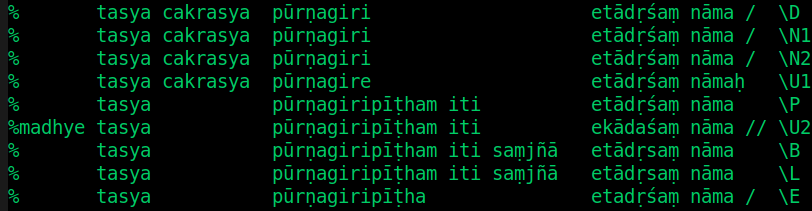
\includegraphics[width=1\textwidth]{pics/synoptic1.png} % Passe die Breite nach Bedarf an
    \caption{Examplee: Synoptic transcription of the \emph{Yogatattvabindu}'s witnesses.}
    \label{fig:synoptic1}
\end{figure}

This one example (Figure \ref{fig:synoptic1}) of one sentence illustrates the broad structural differences as they recur consistently. It became apparent during the transcription of the textual witnesses that the transmission of the text divides into two main branches, each traceable to an archetype.\footnote{Paolo Trovato and others explain the very high rate of lost archetypes and two-branched stemmata by ``the high (90\%) rate of extinction of individual copies'', cf. \citeauthor[2017: 86]{trovato2017}.}
  I refer to the first archetype as \alpha, as its manuscripts predominantly preserve superior readings (\getsiglum{D}, \getsiglum{N1}, \getsiglum{N2}, and \getsiglum{U1}). Thus, these four manuscripts form the \alpha-group. Although this group frequently contains errors, in most cases, there are one or more manuscripts where the reading is entirely convincing. This group also includes the oldest dated manuscript \getsiglum{N1} (1716 CE) from Nepal, of which \getsiglum{N2} is a direct copy. I also collated \getsiglum{N2} as it provided two significant benefits. Firstly, the hand of \getsiglum{N1} is partially difficult to read and, in some places, almost illegible, so \getsiglum{N2}, being very readable, was extremely helpful. Secondly, there are occasional minor discrepancies between the manuscripts, likely corrections by the scribe of \getsiglum{N2}. This scribe had an excellent understanding of the text, and his corrections proved to be useful. Unfortunately, the transmission of the \alpha-group has significant gaps, some of which overlap, resulting in extended text passages where only one witness of the \alpha-group can be relied upon.
  
  I refer to the second archetype as \beta. This group is significant due to the abovementioned circumstances, as its transmission contains almost the entire text with only a few isolated gaps. Among the five available textual witnesses of the \beta-group is the printed edition \getsiglum{E}, based on a hitherto unknown manuscript. The Pandit editor attempted to correct poorly transmitted text passages by his \textit{divinatio}. Unfortunately, apart from some grammatical emendations, he often failed in this endeavour.
  
A further branching of manuscripts splits from the \beta-group, comprising \getsiglum{B} and \getsiglum{L}. These contain the worst and most erroneous transmission of the text by far. Surprisingly, in some rare cases, they provided the decisive and only sensical reading, making their inclusion in the collation indispensable. Overall, the \beta-group is noted for containing additional material in some passages, usually verse insertions that elaborate on a specific term. These were critically edited with the available witnesses and included in the grayscale.

\subsection{Computer Stemmatics applied to the \textit{Yogatattvabindu}}

For the final constitution of the \textit{stemma codicum}, all transcriptions of the entire \emph{Yogatattvabindu} were analyzed using common algorithms from phylogenetic software tools for stemmatic analysis. The dataset was stored in the Nexus format. The numerous gaps in the transmission were coded as non-significant sites in the data to prevent the results from being distorted by the large \textit{lacunae} or the interpolations of the \beta-group, particularly manuscript \getsiglum{U2}. The results were compared with my philological observations, and the findings of both approaches were combined. Here, I present three phylogenetic trees which support and complement my philological considerations. This work serves as an example of how such computer-assisted methods can be applied to stemmatic analysis in a less complex transmission like that of the \emph{Yogatattvabindu}, to create a \textit{stemma codicum} based on empirical data, harmonizing the empiricism of phylogenetic analysis with the expertise of the philologist.\footnote{No computer-generated tree can automatically provide an optimal representation of a text's transmission, cf. \citeauthor{baptiste2020} (2020: 339-356) for an overview of the criticism digital methods have faced since their inception. \citeauthor{maas2009stemma} explains that this arises because the strict bifurcating structure of the computer-generated tree, in which every existing textual witness is connected by exactly one line to a single inferred witness, cannot account for the contamination in the tradition. Furthermore, this bifurcating structure cannot represent cases where some copies were made more than once and more than one copy has survived. In the computer-generated tree, every existing manuscript is represented as a copy of an inferred witness, which is inaccurate; in most text transmissions, numerous manuscripts are copies of other existing manuscripts, see \citeauthor[2009: 80]{maas2009stemma}. This is also true in the case of the \emph{Yogatattvabindu}. If the editor is aware of these issues and can access and modify the deep structures of the computer-generated models to manually identify wrongly assumed bifurcations and contamination, then cladistic analysis with the software used by \citeauthor{maas2009stemma} and his methodology can enable the editor to transform the computer-generated tree into a well-grounded, plausible, and data-based \emph{stemma codicum}.}

\subsubsection{Tree 1: Maximum Parsimony} 

  \begin{figure}[H]
    \centering
    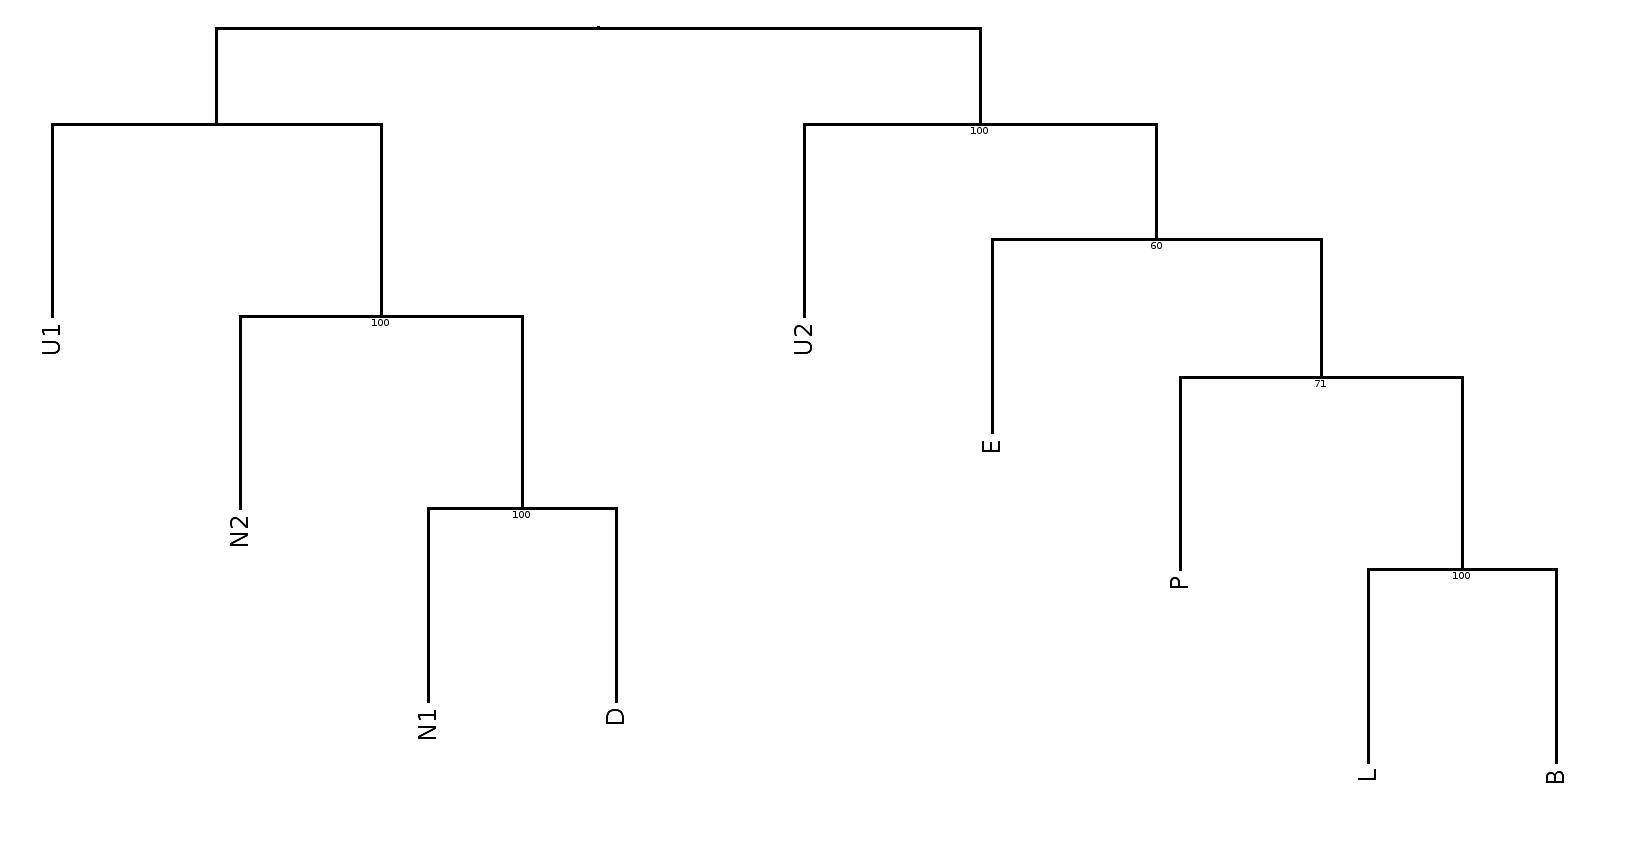
\includegraphics[width=1\textwidth]{pics/paup-tree.png} % Passe die Breite nach Bedarf an
    \caption[Tree 1: Maximum Parsimony]{Mesquite Version 3.81 (build 955). \textbf{Algorithm}: \textit{Parsimony Tree Analysis} with PAUP 4.a168. \textbf{Dataset}: Full collation of the \emph{Yogatattvabindu}.}
    \label{fig:paup-tree}
\end{figure}

The phylogenetic analysis method based on the \textit{Maximum Parsimony} algorithm is one of the most widely used methods for stemmatic analysis in philology.\footnote{\textit{Maximum Parsimony} calculates all possible bifurcating trees and searches for the most parsimonious tree (the one requiring the fewest changes) among them. \textit{Maximum Parsimony} groups manuscripts according to their shared derived characters. Only parsimony informative sites in the data are used for the \textit{Maximum Parsimony} analysis. A site within the data is considered informative if it consists of more than one variant and at least two variants are recorded at least twice. All other sites are excluded, cf. \citeauthor{windram2008} (2008: 445-446).} The tree (Figure \ref{fig:paup-tree}) has an excellent CI (Consistency Index) of 0.869. This means that the proposed tree structure can explain about 87\% of the phylogenetic tree's trait changes. My earlier observation that the manuscripts divide into two main groups was an explicit criterion for placing the root of the tree precisely between these two groups, a division also supported by the \textit{Maximum Parsimony} algorithm. However, this tree has two apparent weaknesses. It does not recognize that \getsiglum{N2} is a direct copy of \getsiglum{N1}. That is because the scribe of \getsiglum{N2} integrated an additional sentence and improved some passages, making the character states closer to those of \getsiglum{U1}. The second weakness, indicated by the relatively low bootstrap score\footnote{Bootstrapping is a method to detect statistical support of phylogenetic trees, see \citeauthor{felsenstein1985} (1985). Bootstrapping is a test to determine whether the whole dataset supports the tree or if the tree is a marginal choice among several almost equal alternatives. That is accomplished by testing the tree with randomized subsamples of the dataset, then building trees from each of these and finally calculating the frequency with which the different parts of the tree are reproduced in each of these random subsamples. The bootstrap support is assigned according to the frequency of a specific group of manuscripts occurring in the subsample trees. If the specific group is found in every subsample tree, then the bootstrap support will be 100\%; if it is found in only half of the subsamples, it will have a bootstrap support of 50\%. Values of 70\% or higher are considered to indicate reliable groupings, cf. \citeauthor{sandra2003} (2003: 250).} of only 60 at the branching where \getsiglum{E} is located, and the bootstrap score of 71 at the branching where \getsiglum{P} is located. That is because the character states resulting from the editorial interventions of the Pandit of the printed edition cannot be smoothly explained by the computer in light of the remaining transmission. Therefore, the positions of \getsiglum{E} and \getsiglum{P} must be carefully considered. The position of \getsiglum{U2} was also surprising. With many interpolations, this manuscript might easily have been underestimated for its stemmatic relevance to the \beta-group. However, its base text (excluding the interpolations) conserves an important transmission stage of the \beta-group.

\subsubsection{Tree 2: Neighbour-joining} 

These are two unrooted Neighbor-joining trees (Figure \ref{fig:nj-tree}). \footnote{\textit{Neighbor-joining} is a particular approach to phylogenetic analysis that SplitsTree can execute. The primary mechanism behind this is a hierarchical clustering technique, see \citeauthor[1987]{nei1987}. A concise explanation by the authors is as follows: ``The principle of this method is to find pairs of operational taxonomic units (OTUs [= neighbours]) that minimize the total branch length at each level of clustering of OTUs starting from a star-shaped tree. The branch lengths and topology of a parsimonious tree can be quickly determined using this method.'' In this case, it can be visualized as follows: The algorithm is fed with a diverse set of texts in the form of manuscript transcripts, which act as operational taxonomic units. \textit{Neighbor-joining} divides them into smaller groups with shared features.
First, the algorithm measures the distance of each possible pair of manuscripts. This distance indicates how different or similar they are regarding specific features. Then, the algorithm finds the two manuscripts with the smallest distance between them. These are the ``closest neighbours'' in terms of similarity. These two individual manuscripts are then joined together to form a node. This node represents an assumed common ancestor. The algorithm then recalculates the distances between this newly created node and all other manuscripts. These distances reflect each manuscript's overall similarity or dissimilarity to the new node. The process repeats and identifies the next pair of nearest manuscripts or groups of manuscripts, creates the next node, and adjusts the distances. In this way, a phylogenetic tree is created. The function repeats these steps until all manuscripts and groups of manuscripts are connected in an undirected tree-like structure in which the length of the branches and the distance between the nodes represent the relationships of the manuscripts based on their similarities. Neighbour-joining assumes a constant rate of evolution across all lineages, and branch lengths correspond to evolutionary distances. The resulting trees can vary considerably depending on how the data are coded and how gaps are treated. The application of \textit{neighbor-joining} to support philological work is discussed by \citeauthor{stemmamethods} (2020: 319).} They are based on the same dataset. The only difference lies in the distance measures used to quantify the evolutionary distance between sequences of \textit{akṣara}s.

These distances are then used to construct phylogenetic trees. The left tree uses the Gene Content Distance,\footnote{The Gene Content Distance is a measure used to compare the presence or absence of genes across different genomes. The distance between two genomes is calculated based on the differences in their gene content, cf. \citeauthor[2004]{huson2004}. Instead of gene content, in our case, the presence or absence of \textit{akṣara}s is compared.} while the right tree uses the standard p-distance, a simple measure of sequence divergence.\footnote{The ``Uncorrected P'' or p-distance calculates the proportion of nucleotide or amino acid sites at which two sequences differ. The calculation of Uncorrected P is simple. The number of differing sites is divided by the total number of sites compared; see \citeauthor[2022: 46]{huson2022}.} The results differ only slightly, but in my assessment, the trees of both distances correspond with key philological observations, particularly regarding the \alpha-group. While the tree using the Gene Content Distance reflects the close relationship between \getsiglum{N1} and \getsiglum{N2}, it does not show that \getsiglum{N1} is the manuscript closest to the archetype \alpha. Conversely, this relationship is correctly depicted in the tree using p-distance (Uncorrected P).

\begin{figure}[H]
    \centering
    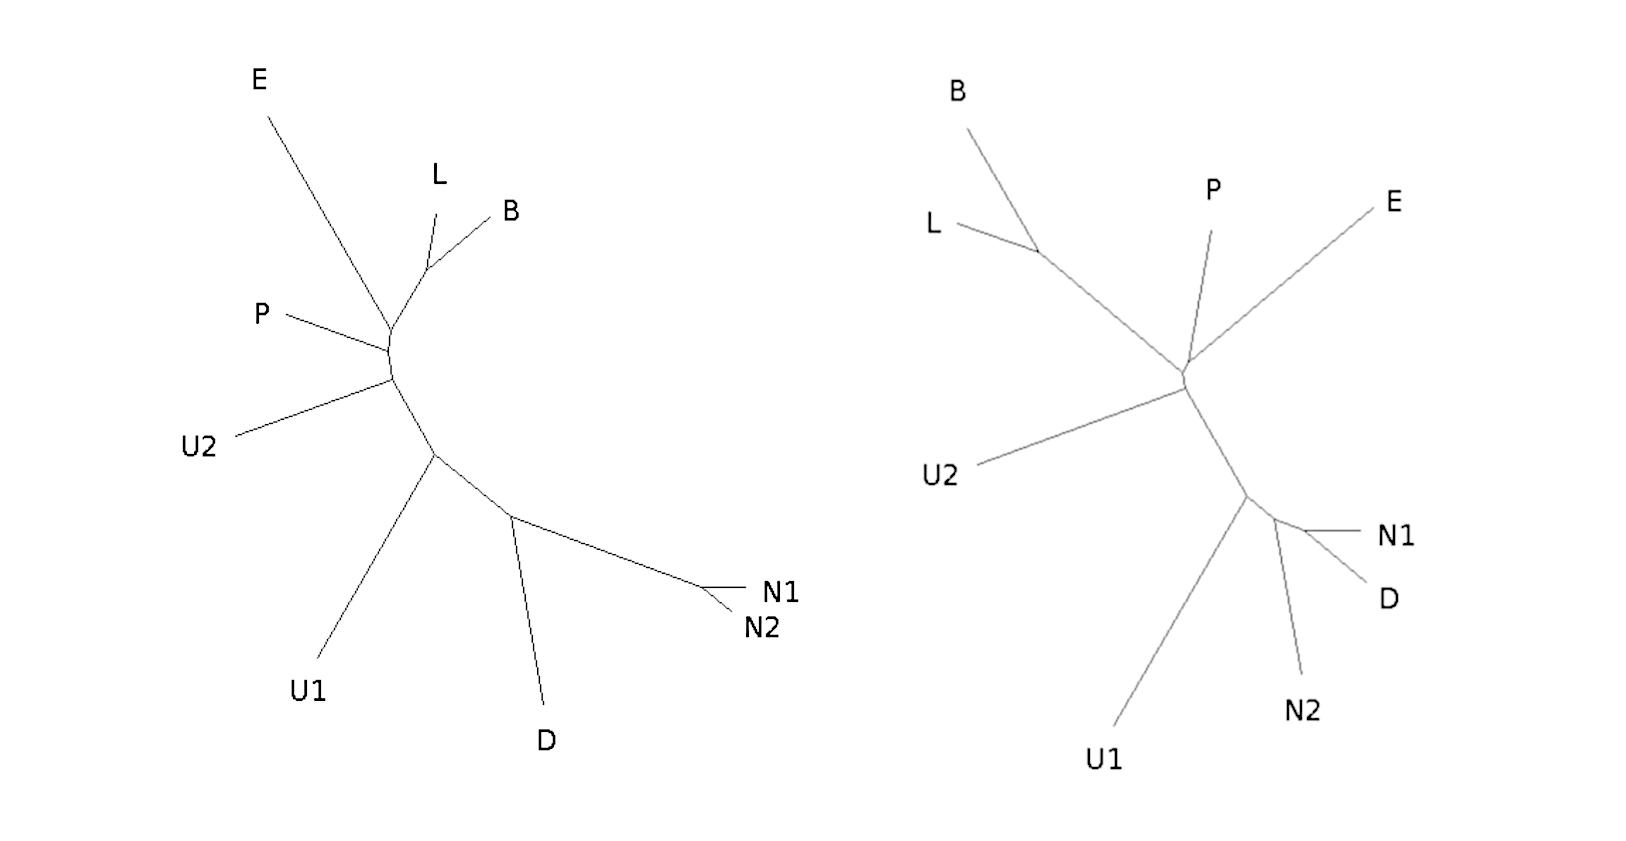
\includegraphics[width=1\textwidth]{pics/tree-nj-x.png} % Passe die Breite nach Bedarf an
    \caption[Tree 2: Neighbour-joining network]{SplitsTree 4 version 4.19.2. \textbf{Algorithm}: \textit{Neighbor-joining} (unrooted). Two trees with identical algorithms and datasets but different distance measures. \textbf{Distance} (left): Gene Content Distance. \textbf{Distance} (right): Uncorrected P. \textbf{Dataset}: Full collation of the \emph{Yogatattvabindu}.}
    \label{fig:nj-tree}
\end{figure}
\newpage
\subsubsection{Tree 3: Minimum Spanning Tree}

Another vital aspect is illustrated by the \textit{Minimum Spanning Tree} (Figure \ref{fig:tree-minspan}).\footnote{The algorithm underlying the \textit{Minimum Spanning Tree} calculates an undirected and unrooted tree-shaped graph representing the simplest way to connect all the manuscripts by minimizing the corresponding nodes based on their pairwise distances, see e.g. \citeauthor{stemmamethods} (2020: 317), \citeauthor{cormen2009introduction} (2009) and \citeauthor{huson2022} (2022: 43). The goal of the \textit{Minimum Spanning Tree} is to calculate the connections between the manuscripts so that the total length to connect all manuscripts settles on the minimum. The \textit{Minimum Spanning Tree} thus, in our use case, represents the simplest and most efficient way to connect a set of manuscripts while minimizing the total distance (based on their differences) of the connections. The resulting tree is far from a stemma and does not include hypothetical ancestral nodes at branching points; any shown branching point corresponds to a manuscript in every case.} A \textit{Minimum Spanning Tree} can help to confirm important manuscripts due to its algorithmic properties. In our case, it highlights the central manuscripts of the two groups, namely \getsiglum{N1} for the \alpha-group and \getsiglum{P} for the \beta-group, which perfectly aligns with the philological observation. Der \textit{Minimum Spanning Tree} Algorithmus wurde nur sehr selten in der Philologie eingesetzt. Weitere Experimente mit verschiedenen Textüberlieferungen deren Stemma bekannt ist, wären nötig, um herauszufinden, ob es sich diese brauchbaren Ergebnisse wiederholen.  

  \begin{figure}[H]
    \centering
    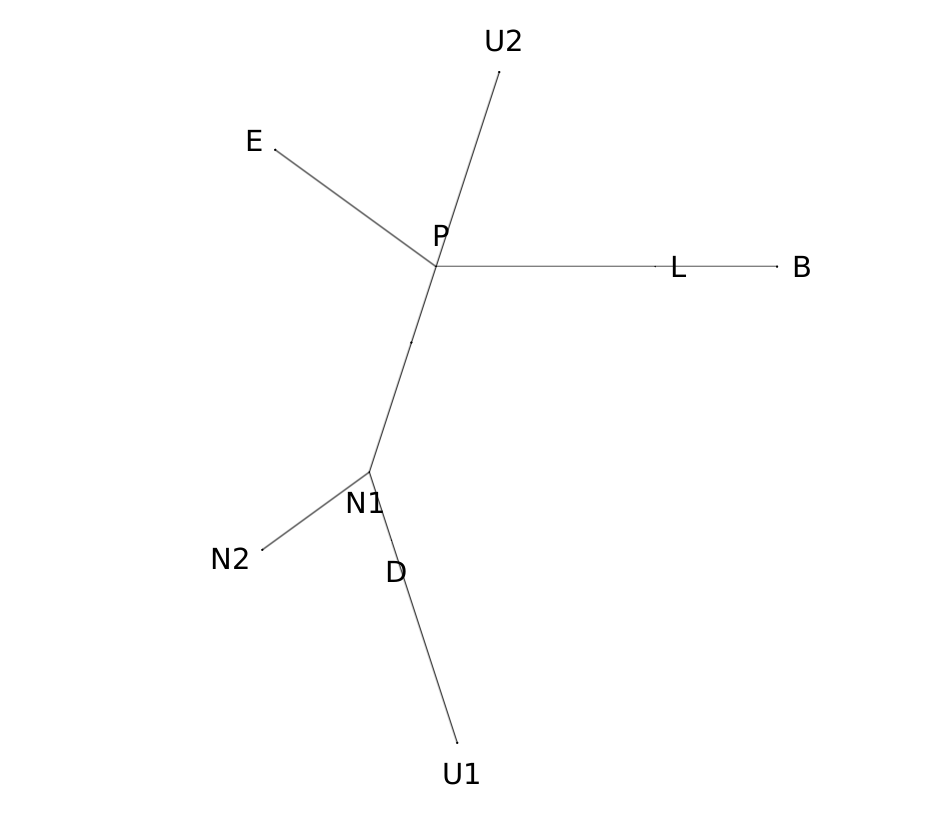
\includegraphics[width=0.6\textwidth]{pics/tree-minspan.png} % Passe die Breite nach Bedarf an
    \caption[Tree 3: Minimum Spanning Tree]{Software: SplitsTree App 6.3.12. Algorithm: \textit{Minimum Spanning Tree}. Distance: Uncorrected P. \textbf{Dataset}: Full collation of the \emph{Yogatattvabindu}.}
    \label{fig:tree-minspan}
\end{figure}

\subsubsection{Stemma codicum}

\begin{figure}[H]
    \centering
    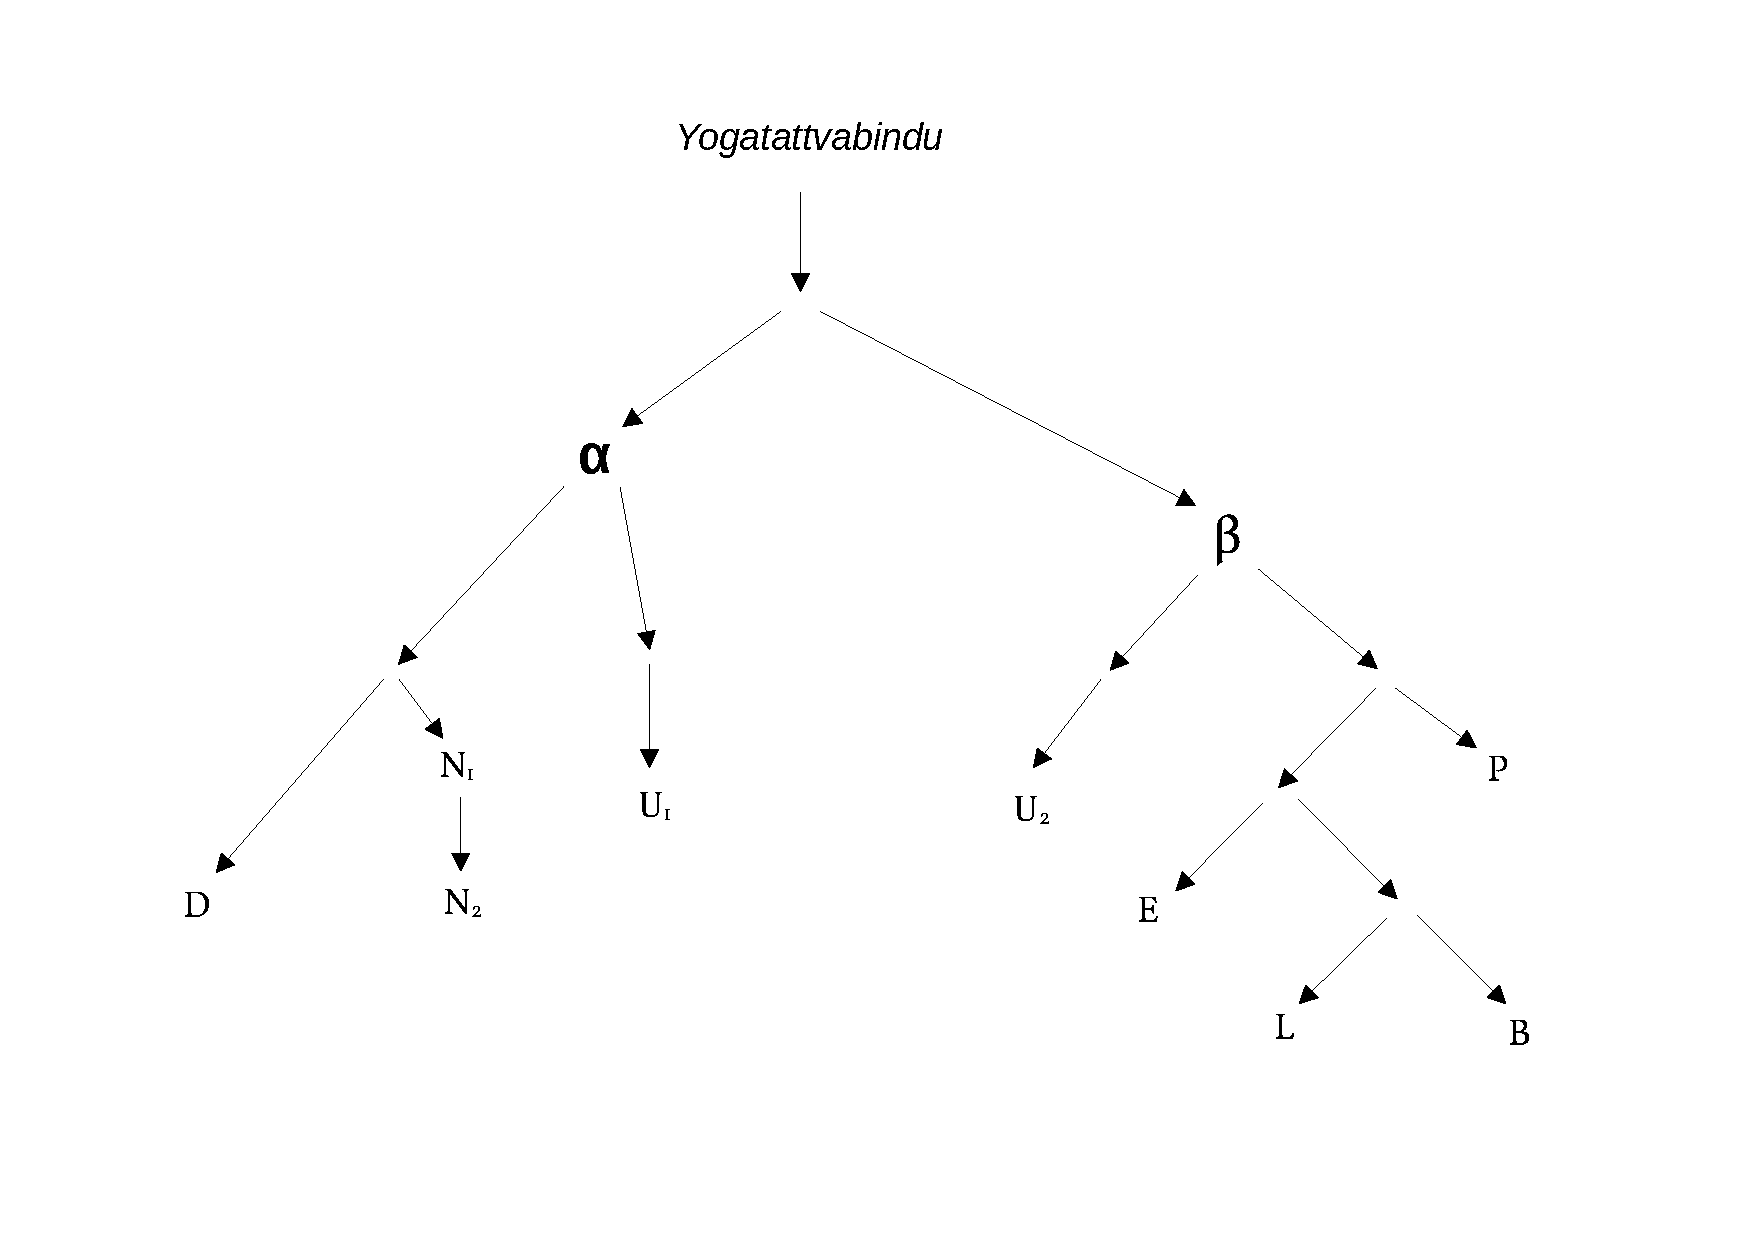
\includegraphics[width=1\textwidth]{pics/stemma.pdf} % Passe die Breite nach Bedarf an
    \caption[Stemmatic hypothesis]{Stemmatic hypothesis of the \emph{Yogatattvabindu}.}
    \label{fig:stemma}
\end{figure}

The cumulative evidence from the phylogenetic algorithms, combined with my philological observations and considerations, leads to the following \textit{stemma codicum} of the \emph{Yogatattvabindu}. This represents a plausible hypothesis of the relationships between the textual witnesses based on the current state of knowledge, forming the foundation upon which the critical edition presented in this dissertation was prepared.

%\footnote{Paolo Trovato and others explain the very high rate of lost archetypes and two-branched stemmata by ``the high (90\%) rate of extinction of individual copies'' \parencite[86]{trovato2017}.}

%- note: U2 must be at the end of the chain of the beta group ... example: The scribe of \getsiglum{U2} tried to save the reading and emended \tetxit{malam} to \textit{param}. Taking the source text's reading into account we can see that \textit{malam} resulted from \textit{nirmalam} and the preceding \emph{kaṃ} could simply be explained as an eyeskip of the preceding Fragepronomen \textit{kaṃ}. (section 45)

%\section{Stylistic Particularities}

% double dandas
% long sentences in list style
% simple sanskrit ...probably because Rāmacandra was Sannyāsi from Daśanāmi and could do not better
% use of genitive
% simple constructions
% only one complex verse Vasantatilaka


\section{Conventions for the critical edition}

\lettrine[lines=2, lhang=0.2, loversize=0.25]{T}{o} enhance reader convenience, the critical edition with its apparatus and the translation together with annotations are presented on facing pages. This arrangement eliminates the need for constant page-turning when the reader wishes to consult the edition, translation, and annotations. While this format offers a significant advantage, it also presents a challenge: the length of the critical edition, including the multi-level critical apparatus on the verso page, does not always match the length of the translation and annotations on the recto page. Despite efforts to minimize this discrepancy, such as shortening annotations, printing empty spaces on one or both pages was often unavoidable.\footnote{This undertaking was laborious, and due to the complexity of the critical apparatus and the evolving technology used in this work, each page had to be manually typeset. This manual process did not achieve the precision that computer-generated typesetting would provide. I decided to typeset the critical edition with the Lua\LaTeX package ``ekdosis,'' see \url{https://ctan.org/pkg/ekdosis}. Ekdosis allows for creating multilingual critical editions with a multi-level critical apparatus and a printable PDF document. The primary reason for this choice is that the entire edition is also output as a TEI-compliant XML file. This file can then be converted into an HTML file, i.e., a digital edition (which I hope to publish soon for the \emph{Yogatattvabindu}) with the press of a button using a script and an XSLT processor, facilitating computer-aided stemmatic analysis, data mining, and similar tasks. I want to thank Robert Alessi for his incredible support. I hope that ekdosis, which holds great potential for philologists seeking to leverage digital humanities, will continue to be developed and enable automatic page breaks of a complex multi-layered critical apparatus in an alignment environment of facing pages with translation and annotation. I hope some readers will appreciate the effort made to provide the convenience of not having to flip between the edition, translation, and annotations in my edition.}

The constituted text of the critical edition has been set in modern Devanāgarī, reflecting the vast majority of manuscripts and presumably the original text of the \textit{Yogatattvabindu}.
The editor introduced the headings and section numbering in large Roman numerals within square brackets to organize the text, make the beginning of new topics clear, and facilitate citation. These headings correspond to the sections introduced in the text by recognizable phrases such as \textit{atha}, \textit{idānīṃ}, and the like. Rāmacandra did not distinguish between chapters, subchapters, sections, and subsections but instead linked themes with these phrases. The headings in square brackets follow this convention. The verse numbering begins with the section numbering and subsequently counts the number of verses per section.
Among the text's witnesses, there is a deviating and inconsistent application of \textit{sandhi}. For the edition text, I have standardized \textit{sandhi} and, when necessary, added \textit{avagraha}s to provide a readable text adhering to contemporary conventions in Sanskrit. The variant readings concerning \textit{sandhi} are consistently recorded in the apparatus criticus. That is due to various text-critical problems\footnote{The inconsistent use of punctuation marks in the available witnesses necessitates standardization. Upon close examination, it appears that punctuation has frequently been dropped or added during the transmission of the texts. The copyists' neglect or improper handling of punctuation has resulted in different versions of lists with and without punctuation. In many instances, missing punctuation has led to the change of case endings, alteration of the text, and the combination of list items into compound formations that were not present in the original text.} arising from the inconsistent usage of punctuation, which results in the application or non-application of \textit{sandhi} depending on whether the respective witness applied a \textit{daṇḍa} or not. That is particularly the case within lists, which frequently occur in our compilation. Items were most likely originally separated by double \textit{daṇḍa}s.

These lists are a frequent feature in the \textit{Yogatattvabindu}. The text opens with a list of 15 Yogas, and many more lists are utilized throughout its content. In order to produce a consistent and easily readable edition, lists have been normalized to the nominative singular or nominative plural form of the respective item, or, in the case of explanatory lists, to the ablative singular or plural. The items of the lists are always separated by a double \textit{daṇḍa}.

The critical edition follows the standard conventions of punctuation. In verse poetry, a \textit{daṇḍa} (|) marks the end of a half-verse or quarter of the \textit{śloka}, and a double \textit{daṇḍa} (||) marks the end of a verse. In prose, a single \textit{daṇḍa} indicates the end of a sentence, and a double \textit{daṇḍa} marks the end of a section. In most cases, the \textit{daṇḍa} in prose corresponds to a full stop.

Furthermore, I have standardized gemination and degemination of consonants after semi-vowels. Due to the inconsistent use of class nasals among the witnesses, \textit{anusvāra}s have been substituted with the respective class nasals throughout the edition.

\subsection{Grammatical particularities}

Grammatical constructions in this text may deviate from classical Sanskrit. In most cases, however, these should not be regarded as errors due to their frequency but as phenomena of contemporary or regional language usage. Some passages of the text use the genitive as a substitute for other cases, such as the dative, instrumental or locative (cf. \citeauthor{whitney1879} 1879: 87 [294]). In particular, this can be observed in this and other places in the text in relative clause constructions beginning with \textit{yasya}, which must be read as \textit{yasmin}, as otherwise, the corresponding correlative pronoun seems to be missing. The genitive, for example, in connection with the following word \textit{manasi} or \textit{manaḥ} (see edition text) would make the yogin the implicit subject of the sentence and the actual correlative pronoun of the construction referring to \textit{yasya}, in this section \textit{ayam} or \textit{saḥ}, would appear incongruent. A \textit{daṇḍa} must often be read as a comma in these relative clause constructions.

\subsection{Guide to the apparatus}

The critical apparatus consists of five layers, not all of which are populated on each page. These are sources, testimonia, parallels, the critical apparatus with readings of the witnesses, and notes. To facilitate the differentiation of sources, testimonia, and parallels for the reader, these are marked as such on each page where they occur, aside from the critical apparatus.

The numbering of all layers of the apparatus and the lemmata follows the line numbering. This applies to both prose passages and verses. Every line is counted, and every fifth line of the text is numbered on the far left margin. The numbering is bold and blue to aid the reader's navigation in the apparatus.
When present, the first layer of the apparatus displays the source texts. It should be noted that Rāmacandra does not adopt the sources verbatim but often converts verses into prose and occasionally adds or omits information according to his agenda. When Rāmacandra incorporates verses, he usually makes editorial changes. According to the schema, variables in the source texts are indicated in round brackets following the affected word.

In the second layer, if available, testimonia are recorded. In the third layer, if available, parallel passages that are helpful or informative for the reconstruction of the text are noted. All texts used in these first three layer are consistently cited. If these texts are only available in manuscript form, the entry begins with the title, followed by an abbreviation for the location, the Ms. No., in round brackets (e.g., MMPP 2244 f. 99r l. 1-2). When the passage of the source, the testimonia or the parallel is identical, it is preceded by the equal sign (=). The approximate sign (\approx) is used instead when the passage is approximate to a certain degree. 

The fourth layer contains the critical apparatus. The critical apparatus is positive. Each lemma begins with the corresponding line number, followed by the selected reading. The selected reading is followed by one or more sigla that contain this reading. The closing square bracket separates this from the variants that follow. These are presented with the reading followed by the siglum. The selected reading is always highlighted in bold. The abbreviation ``cett.'' has been introduced to keep the critical apparatus concise. It stands for the Latin \textit{ceteri}, meaning literally ``the rest,'' and refers to all other witnesses except those named for each lemma. This entry can appear only once per lemma. Here is an example:

\begin{quote}
  \textbf{indriyavikāraḥ} cett.] iṃdriyaṃ vīkāraḥ P iti vikāraḥ L
  \end{quote}

When the selected reading results from a correction (corr.), an emendation (em.), or a conjecture (conj.), the corresponding abbreviation appears instead of a witness, a group of witnesses (\alpha or \beta), or the \textit{ceteri} abbreviation before the square bracket. If the emendation or conjecture is attributed to a colleague, the colleague's surname is printed in uppercase letters before the abbreviation. If the reasoning behind the conjecture is not self-explanatory, it is explained in the annotations. The plus sign (+) represents illegible or missing letters due to manuscript damage. Given the manageable number of textual witnesses, all variants are recorded in the lemmata of the critical apparatus. If words or sentences are omitted (om.), this is always noted in the corresponding entry before the respective siglum.
However, in cases of larger \textit{lacunae}, such as the \textit{lacunae} in \getsiglum{N1} and \getsiglum{N2}, which encompass 23,50\% of the total text, I have opted to omit to record each omission in the apparatus for the sake of a more concise critical apparatus. For these cases, I have documented this in the last register of the apparatus, which informs about the beginning and end of larger gaps in the text, with a note that the large \textit{lacunae} for this section are not included in the critical apparatus. In addition to comments regarding omissions, the last layer also contains information about transpositions of passages and other such details.
According to the conventions of recent publications of critical editions of Yoga texts\footnote{See, for example, \emph{Amṛtasiddhi} (2021), \emph{Śivayogapradīpikā} (2023), or \emph{Amaraugha} and \emph{Amaraughaprabodha} (2024).}, the lemmata in the critical apparatus, as well as all sources, testimonia, and parallels, are set in Roman transliteration.

\subsection{Guide to the translation and annotations}

The translation is arranged parallel to the critical edition on the recto side of the book. In the translations, I have endeavoured to reflect the style of Sanskrit. Thus, I have sought to balance literal and idiomatic translation well. Verse insertions have been enumerated according to the numbering of the sections and clearly marked as such. When translations of certain words derive from a secondary or tertiary meaning, and the significance is not immediately apparent, the Sanskrit term is noted in round brackets. Technical terms from Sanskrit or proper names have not been translated into English. Technical terms with various possible translations, whose meaning can only be discerned in the context of the entire text, are printed in Sanskrit but accompanied by a translation in round brackets. English words that had to be added to facilitate the translation or provide contextual information that was not immediately evident are integrated into the translation in square brackets. The footnotes discuss textual issues, provide additional information, explain technical terms, or highlight important or interesting parallels to other texts.

%The following procedure emerged for the constitution of the critical edition. When the readings of both groups coincided, this was always a strong indication in favour of adopting the respective reading. When the groups differed, the \alpha-group was generally preferred if it was reasonable and grammatically correct. However, if the \alpha-group contained undoubtedly corrupted readings and the \beta-group offered sensible and correct alternatives, readings from the \beta-group were adopted after careful examination. In rare cases where the text was so corrupt that emendation or conjecture was necessary, appropriate adjustments were made.

\subsection{Abbreviations and signs}
\begin{itemize}
\item[Ed.]  Edition
\item[Ibid.]  Ibidem
\item[em.]  emendation
\item[conj.]  conjecture
\item[corr.]  correction
\item[BIRCH]  Jason Birch
\item[HANNEDER]  Jürgen Hanndeder
\item[MALLINSON]  James Mallinson
\item[SELLMER]  Sven Sellmer  
\item[unm.]  unmetrical
\item[illeg.]  illegible
\item[f.]  folio
\item[ff.]  folios
\item[r]  recto
\item[v]  verso
\item[l.]  line
\item[ll.]  lines
\item[et seqq.] et sequentia (``and those following'')
\item[Ms.]  Manuscript
\item[Mss.]  Manuscripts
\item[Ms. No.]  Manuscript number 
\item[YTB] \emph{Yogatattvabindu} 
\item[YSv] \emph{Yogasvarodaya}
\item[SSP] \emph{Siddhasiddhāntapaddhati}
\item[YK] \emph{Yogakarṇikā}
\item[ŚKD] \emph{Śabdakalpadruma} 
\item[NGMCP] Nepalese German Manuscript Cataloguing Project
\item[NGMPP] Nepalese German Manuscript Preservation Project
\item[IGNCA] Indira Gandhi National Centre for the Arts (Delhi)
\item[SORI] Scindia Oriental Research Institute Vikram University (Ujjain)
\item[ORI] Oriental Research Institute (Mysore) 
\item[GOML] Government Oriental Manuscript Library (Chennai)
\item[MMPP]  Maharaja Man Singh Pustak Prakash Research Centre
\item[PULL]  Panjab University Library Lahore
\item[IFP] French Institute of Pondicherry 
\item[+] illegible letter (++ = one \textit{akṣara}) 
\item[\Large{\textbf{†}}] marks the beginning and end of an
\item[=] passage or verse is identical
\item[\approx] passage of verse is similar
\end{itemize}

\subsection{Sigla in the critical apparatus}

\begin{itemize}
\item \alpha : \getsiglum{D}, \getsiglum{N1},  \getsiglum{N2}, \getsiglum{U1}
\item \beta : \getsiglum{B}, \getsiglum{E},  \getsiglum{L}, \getsiglum{P}, \getsiglum{U2}
\item cett.: ceteri (all manuscripts except the ones mentioned in the lemma)
\item E : Printed Edition
\item P : Pune BORI 664
\item L : Lalchand Research Library LRL5876
\item B : Bodleian Oxford D 4587
‚\item \None : NGMPP B 38-31
\item \Ntwo : NGMPP B 38-35 / A 1327-14
\item \Done : IGNCA 30019
\item \Uone : SORI 1574
\item \Utwo : SORI 6082
\item YK : \emph{Yogakarṇikā}
\item YSv : \emph{Yogasvarodaya}
\item PT : \emph{Prāṇatoṣiṇī}
\end{itemize}

\chapter{Critical Edition \& Annotated Translation}
\cleardoublepage
\begin{alignment}[
  texts=edition[class="edition"];
  translation[class="translation"],
  ]
  \begin{edition}
    \ekddiv{
      head={[\uproman{1}. \textbf{rājayogaprakāra}]},
      type=section,
      depth=2,
      n=I
    }
    \xmlhead[h01]{[I. rājayogaprakāraḥ]}
    \addcontentsline{toc}{section}{I. rājayogaprakāraḥ}
\label{intro}
\begin{prose}[p01_01]
\noindent
%--------------------------
% śrīgaṇeśāya namaḥ /                                                     rājayogāntargataḥ //  binduyogaḥ   \E 
% śrīgaṇeśāya namaḥ /                                                     atha tattvabiṃduyogaprāraṃbhaḥ     \L
% śrīṇe ya maḥ /                                                          atha rājayoga         liṣyate      \P
% \om                                                                                                         \B      
% śrīgaṇeśāya namaḥ // śrī gurave namaḥ //                                atha rājayogaprakāro  likhyate //  \N1
% śrīgaṇeśāya namaḥ //                                                //  atha rājayogaprakāro  likhyate //  \N2
% śrīgaṇeśāya namaḥ // śrī sarasvatyai namaḥ // śrī nirañjanāya namaḥ //  atha rājayogaprakāro  likhyate //  \D
% śrīgaṇeśāya namaḥ /  oṃ śrī niraṃjanāya //                              atha rājayogaprakāra  likhyate //  \U1
% śrīgaṇeśāya namaḥ /                                                     atha rājayoga         likhyate //  \U2
%--------------------------
%Homage to Śrī Gaṇeśa. Now, the way of Rājayoga is laid down.
%--------------------------          
\note[type=source, labelb=_0b,labele=_00e, nosep]{cf. YSv (PT p. 831): atha rājayogaḥ || yogasvarodaye | īśvara uvāca | rājayogaṃ pravakṣyāmi śṛṇu sarvatra siddhidam | guhyād guhyataraṃ devi nānādharmaṃ parāt param rājayogena deveśi nṛpapūjyo bhaven naraḥ | rājayogī cirāyuś ca aṣṭaiśvaryamayo bhavet ||}
\app{\lem[wit={ceteri}]{śrīgaṇeśāya namaḥ}\linelabel{_0b}
        \rdg[wit={P}]{śrīṇeyamaḥ}
        \rdg[wit={N1}]{śrīgaṇeśāya namaḥ || śrīgurave namaḥ ||}
        \rdg[wit={D}]{śrīgaṇeśāya namaḥ || śrīsarasvatyai namaḥ || śrīnirañjanāya namaḥ ||}
        \rdg[wit={U1}]{śrīgaṇeśāya namaḥ || oṃ śrīniraṃjanāya ||}}\dd{}
\app{\lem[wit={D,N1,N2}]{atha rājayogaprakāro likhyate}
        \rdg[wit={U1}]{atha rājayogaprakāra likhyate}
        \rdg[wit={E}]{rājayogāntargataḥ || binduyogaḥ}
        \rdg[wit={L}]{atha tattvabiṃduyogaprāraṃbhaḥ}
        \rdg[wit={P}]{atha rājayoga liṣyate}
        \rdg[wit={U2}]{atha rājayoga likhyate}}/ 
%-------------------------- 
% \om                        \E
% \om                        \L
% \om                        \B
% rājayogasyedaṃ phalaṃ      \P
% rājayogasya idaṃ phalaṃ    \N1
% rājayogasya idaṃ phalaṃ    \N2
% rājayogasya idaṃ phalaṃ // \D
% rājayogasya idaṃ phalaṃ    \U1
% rājayogasyedaṃ phalaṃ /    \U2
%--------------------------    
\app{\lem[wit={P,U2}]{rājayogasyedaṃ phalaṃ}
  \rdg[wit={D,N1,N2}]{rājayogasya idaṃ phalaṃ}
  \rdg[wit={E,L}]{\om}}
%--------------------------
%This is the result of \textit{rājayoga}:
%--------------------------
% \om                                                                                                                                                                         \E
% \om                                                                                                                                                                         \L
% \om                                                                                                                                                                         \B
% yena rājayogenāneka---rājyabhogasamaya   eva   anekapārthivavinodaprekṣaṇasamaya  eva   bahutarakālaṃ  śarīrasthitir  bhavati    sa eva  rājayogaḥ tasyaite     bhedāḥ      \P
% yena rājayogenāneka---rājyabhogasamaya   eva/  anekapārthivavinodaprekṣaṇasamaya  eva/  bahutarakālaṃ  śarīrasthitir  bhavati    sa eva  rājayogaḥ /  tasya ete bhedāḥ /    \N1
% yena rājayogena  anekarājyabhogasamaya   eva// anekapārthivavinodaprekṣaṇasamaya  eva   bahuttarakālaṃ śarīrasthitir  bhavati    sa eva  rājayogaḥ /  tasya ete bhedāḥ /    \N2
% yena rājayogena  anekarājyabhogasamaya   eva// anekapārthivavinodaprekṣaṇasamaya  eva// bahutarakālaṃ  śarīrasthitir  bhavati//  sa eva  rājayogaḥ // tasya ete bhedāḥ /    \D
% yena rājayogena  anekarājyabhogasamaya   eva// anekapārthivavinodaprekṣaṇasamaya  eva// bahutarakālaṃ  śarīrasthitir  bhavati    sa evaṃ rājayogaḥ    tasya ete bhedāḥ //   \U1 
% yena rājayogena  anekarājyabhogasamaya   eva// anekapārthivavinodaprekṣyaṇasamaya eva// bahutarakālaṃ  śarīrasthitir  bhavati//  sa eva  rājayogastaisyaite     bhedāḥ //   \U2
% --------------------------
%\textit{Rājayoga} is that by which longterm durability of the body arises even amongst manifold royal pleasures even amongst the manifold royal entertainments and spectacle. This truly is \textit{rājayoga}. Of this [\textit{rājayoga}] these are the varieties: \end{tlate}
%--------------------------
yena rāja\app{\lem[wit={P,N1}, alt={°yogenāneka°}]{yogenāneka}
  \rdg[wit={D,N2,U1,U2}]{°yogena aneka°}
}rājya:\\bhogasamaya eva anekapārthivavinoda\app{\lem[wit={ceteri}, alt={°prekṣaṇasamaya}]{prekṣaṇasamaya}
        \rdg[wit={U2}]{prekṣyaṇasamaya}}
      eva bahutarakālaṃ śarīrasthitir-bhavati/
      sa \app{\lem[wit={ceteri}]{eva}
        \rdg[wit={U2}]{evaṃ}}
      \app{\lem[wit={ceteri}, alt={rājayogaḥ}]{rājayo:\\gaḥ}
        \rdg[wit={U2}]{rājayogas}}/ 
      \app{\lem[wit={P,U2}]{tasyaite}
        \rdg[wit={ceteri}]{tasya ete}} bhedāḥ/\linelabel{_00e}
        \note[type=source, labelb=_1b, labele=_1e, nosep]{cf. YSv (PT p. 831): pañcadaśaprakāro 'yaṃ rājayogaḥ || kriyāyogo jñānayogaḥ karmayogo haṭhas tathā | dhyānayogo mantrayoga urayogaś ca vāsanā |  rājaty etad brahmavaśīva ebhiś ca pañcadaśadhā | idānīṃ lakṣaṇañ caiṣāṃ kathayāmi śṛṇu priye |}
        \note[type=analogia, labelb=_1b, labele=_1e, nosep]{ cf. \textit{Yogasiddhāntacandrikā} (Ed. p. 2): nididhyāsanañ caikatānatādirūpo rājayogāparaparyāyaḥ samādhiḥ | tatsādhanaṃ tu kriyāyogaḥ, caryāyogaḥ, karmayogo, haṭhayogo, mantrayogo, jñānayogaḥ, advaitayogo, lakṣyayogo, brahmayogaḥ, śivayogaḥ, siddhiyogo, vāsanāyogo, layayogo, dhyānayogaḥ, premabhaktiyogaś ca |}
%-------------------------
%
% \om                                                                                                                                                                \E
% \om                                                                                                                                                                \L
% \om                                                                                                                                                                \B
% kriyāyogaḥ 1 jñānayogaḥ 2 caryāyogaḥ 3 haṭhayogaḥ 4 karmayogaḥ 5 layayogaḥ 6 dhyānayogaḥ 7 maṃtrayogaḥ 8 lakṣyayogaḥ 9 vāsanāyogaḥ 10 śivayogaḥ 11 brahmayogaḥ 12 advaitayogaḥ 13 siddhayogaḥ 14 rājayogaḥ 15 ete paṃcadaśayogāḥ \P
%
% kriyāyogaḥ / jñānayogaḥ / caryāyogaḥ / haṭhayogaḥ / karmayogaḥ / layayogaḥ / dhyānayogaḥ / maṃtrayogaḥ / lakṣyayogaḥ / vāsanāyogaḥ / śivayogaḥ / brahmayogaḥ / advaitayogaḥ / rājayogaḥ / siddhayogaḥ / ete paṃcadaśayogāḥ // \N1
%
% kriyāyogaḥ jñānayogaḥ caryāyogaḥ haṭhayogaḥ karmayogaḥ layayogaḥ dhyānayogaḥ maṃtrayogaḥ lakṣayogaḥ vāsanāyogaḥ śivayogaḥ brahmayogaḥ advaitayogaḥ rājayogaḥ siddhayogaḥ // ete paṃcadaśayogāḥ // \N2      
%      
% kriyāyogaḥ // jñānayogaḥ // caryāyogaḥ // haṭhayogaḥ // karmayogaḥ // layayogaḥ // dhyānayogaḥ // maṃtrayogaḥ // lakṣyayogaḥ // vāsanāyogaḥ // śivayogaḥ // brahmayogaḥ // advaitayogaḥ // rājayogaḥ // siddhayogaḥ // ete paṃcadaśayogāḥ // \D
% \om                                                                                                                                                                         \D2      
%
% kriyāyogaḥ // jñānayogaḥ // tvaryāyogaḥ // haṭhayogaḥ // karmayogaḥ // layayogaḥ // dhyānayogaḥ maṃtrayogaḥ  lakṣayogaḥ  vāsanāyogaḥ  śivayogaḥ  brahmayogaḥ  advaitayogaḥ  rājayogaḥ  siddhayogaḥ ete paṃcadaśayogāḥ  \U1
%
% kriyāyogaḥ // jñānayogaḥ // caryāyogaḥ // haṭhayogaḥ // karmayogaḥ // nayayogaḥ // dhyānayogaḥ // maṃtrayogaḥ // lakṣyayogaḥ // vāsanāyogaḥ // śivayogaḥ // brahmayogaḥ // advaitayogaḥ // siddhayogaḥ // rājayogaḥ // evaṃ paṃcadaśāyogā bhavaṃti // \U2
%-------------------------
         kriyāyogaḥ 1\dd{}\linelabel{_1b}
         jñānayogaḥ 2\dd{}
         \app{\lem[wit={ceteri}]{caryāyogaḥ}
          \rdg[wit={U1}]{tvaryāyogaḥ}} 3\dd{}
        haṭhayogaḥ 4\dd{}
        karmayogaḥ 5\dd{}
        \app{\lem[wit={ceteri}]{layayogaḥ}
          \rdg[wit={U2}]{nayayogaḥ}} 6\dd{}
        dhyānayogaḥ 7\dd{}
        mantrayogaḥ 8\dd{}
        \app{\lem[wit={ceteri}]{lakṣyayogaḥ}
          \rdg[wit={U1}]{lakṣayogaḥ}} 9\dd{}
        vāsanāyogaḥ 10\dd{}
        śivayogaḥ 11\dd{} 
        brahmayogaḥ 12\dd{}
        advaitayogaḥ 13\dd{} 
        \app{\lem[wit={P,U2}]{siddhayogaḥ}
          \rdg[wit={X}]{rājayogaḥ}} 14\dd{}
        \app{\lem[wit={P,U2}]{rājayogaḥ}
          \rdg[wit={ceteri}]{siddhayogaḥ}} 15\dd{}     
        \app{\lem[wit={D,N1,P,U1}]{ete pañcadaśayogāḥ}
          \rdg[wit={U2}]{evaṃ paṃcadaśāyogā bhavaṃti}}\dd{}\linelabel{_1e}
      \end{prose}
      \ekddiv{
        head={[\uproman{2}. \textbf{kriyāyogasya lakṣaṇam}]},
        type=section,
        depth=2,
        n=II
      }
      \xmlhead[h02]{[II. kriyāyogasya lakṣaṇam]}
          \addcontentsline{toc}{section}{II. kriyāyogasya lakṣaṇam}
\label{kriyayogastart}
%--------------------------        
% \om                                      \E
% \om                                      \L
% \om                                      \B
% idānīṃ kriyāyogasya lakṣaṇaṃ kathyate/   \P
% idānīṃ kriyāyogasya lakṣaṇaṃ kathyate/   \N1
% idānī  kriyāyogasya lakṣaṇaṃ kathyate//  \N2
% idānīṃ kriyāyogasya lakṣaṇaṃ kathayate/  \D
% \om                                      \D2
% idānīṃ kriyāyogasya lakṣaṇaṃ kathyate/   \U1
% atha   kriyāyogas   lakṣaṇaṃ          // \U2
%--------------------------
%Now, the characteristic of the Yoga of [mental] action (\textit{kriyāyoga}) described.
%--------------------------
\begin{prose}[p02_01]
\noindent
        \app{\lem[wit={ceteri}]{idānīṃ}
            \rdg[wit={N2}]{idānī}
            \rdg[wit={U2}]{atha}}
          \app{\lem[wit={ceteri}]{kriyāyogasya}
            \rdg[wit={U2}]{kriyāyogas}} lakṣaṇaṃ
          \app{\lem[wit={ceteri}]{kathyate}
            \rdg[wit={D}]{kathayate}
            \rdg[wit={U2}]{\om}}/
\end{prose}
\begin{tlg}[02_1]
  \noindent
%--------------------------   
% \om                                                    \E
% \om                                                    \L
% \om                                                    \B
% kriyāmuktir    ayaṃ yogaḥ    svapiṇḍe siddhidāyakaḥ    \P
% kriyāmuktir    ayaṃ yogaḥ /  svapiṇḍe siddhidāyakaḥ /  \N1
% kriyāmukti    layaṃ yogaḥ    svapiṇḍe siddhidāyakaḥ /  \N2
% kriyāmuktir    ayaṃ yogaḥ    svapiṇḍe siddhidāyakaḥ /  \D
% \om                                                    \D2
% kriyāyuktir    ayaṃ yogaḥ /  svapiṇḍe siddhidāyakaḥ /  \U1
% kriyāmuktiḥ // ayaṃ yogaḥ    svapiṇḍe siddhidāyakaṃ // \U2 
%--------------------------
%This Yoga is liberation through [mental] action, it bestows success(\textit{siddhi}) in ones own body.
%-------------------------- 
   \tl{\note[type=source, labelb=4, labele=_4e, nosep]{ \approx  YSv (PT p. 831): kriyāmuktimayo (\textit{kriyāmuktir ayaṃ} YK 1.209) yogaḥ sapiṇḍisiddhidāyakaḥ (\textit{sapiṇḍe} YK 1.210) | yat kāromīti (\textit{karomīti} YK 1.210) saṅkalpaṃ kāryārambhe manaḥ sadā ||}
     \app{\lem[wit={ceteri}, alt={kriyāmuktir}]{kriyāmukti\skp{r-a}}
    \rdg[wit={N2}]{kriyāmukti}
    \rdg[wit={U2}]{kriyāmuktiḥ ||}
}\app{\lem[wit={ceteri}, alt={ayaṃ}]{\skm{r-a}yaṃ}
  \rdg[wit={N2}]{layaṃ}}
yogaḥ svapiṇḍe
\app{\lem[wit={ceteri}]{siddhidāyakaḥ}
  \rdg[wit={U2}]{siddhidāyakaṃ}}/}\\
%-------------------------
% \om                                                    \E
% \om                                                    \L
% \om                                                    \B
% yaṃ yaṃ karoti kallolaṃ kāryāraṃbhe manaḥ sadā         \P
% yaṃ yaṃ karoti kallolaṃ kāryāraṃbhe manaḥ sadā/        \N1
% yaṃ yaṃ karoti kallolaṃ kāryāraṃbhe manaḥ sadā//1//    \N2
% yaṃ yaṃ karoti kallolaṃ kāryāraṃbhe manaḥ sadā/        \D
% \om                                                    \D2
% yaṃ yaṃ karoti kallolaṃ kāryāraṃbhe manaḥ sadā/ 1      \U1
% yaṃ yaṃ karoti kallolaṃ kāryāraṃbhe manaḥ sadā/        \U2
%--------------------------
%Each wave the mind creates at the beginning of an action,
%-------------------------- 
\tl{yaṃ yaṃ karoti kallolaṃ kāryāraṃbhe manaḥ sadā/}\\\linelabel{_4e}
%--------------------------
% \om                                                        \E
% \om                                                        \L
% \om                                                        \B
% tattataḥ   kuñcanaṃ kurvan kriyāyogas tato bhavet            \P
% tattataḥ   kuñcanaṃ kurvan kriyāyogas ato bhava     //       \N1
% tattataḥ   kūrcanaṃ kurvan kriyāyogas ato bhava     //       \N2
% tattataḥ   kuñcanaṃ kurvan kriyāyogas ato bhava     //       \D
% \om                                                          \D2
% taṃ kṛtaṃ  kuñcanaṃ kurvan kriyāyogas ato ?va      //1//    \U1
% tatastataḥ kuṃcanaṃ kurvan kriyāyogas tato bhavet //1//     \U2
%--------------------------
% ??? . Then \textit{kriyāyoga} arises.
%--------------------------
\note[type=source, labelb=_4b, nosep]{ \approx  YSv (PT p. 831): tatsāṅgācaraṇaṃ (\textit{°saṅgā°} YK 1.210) kurvan kriyāyogarato bhavet |}
\tl{\app{\lem[type=emendation, resp=mallinsonem, alt={tat tat}]{tat-ta\skp{t-ā}}
    \rdg[wit={D,N1,N2,P}]{tattataḥ}
    \rdg[wit={U2}]{tatas tataḥ}
    \rdg[wit={U1}]{taṃ kṛtaṃ}
}\app{\lem[type=emendation, resp=mallinsonem, alt={ākuñcanaṃ}]{\skm{t-ā}kuñcanaṃ}\linelabel{_4b}
    \rdg[wit={D,P,N1,U1,U2}]{kuñcanaṃ}
    \rdg[wit={N2}]{kūrcanaṃ}}
  kurvan-kriyāyoga\skp{s-ta}\app{\lem[wit={P,U2}, alt={tato bhavet}]{\skm{s-t}ato bhavet}
    \rdg[wit={D,N1,N2}]{ato bhava}
    \rdg[wit={U1}]{ato ++va}}\dd{}\begin{otherlanguage}{english}\uproman{2}.1\end{otherlanguage}\hskip-2pt\dd{}}\linelabel{_4e}
\end{tlg}
\end{edition}
\begin{translation}
  \ekddiv{
    head={[\uproman{1}. \textbf{Method of Rājayoga}]},
    type=section,
    depth=2,
    n=I.1
  }
\xmlheadtrans[h01]{[I. Method of Rājayoga]}
\label{introtrans}
\begin{tlate}[p01_01]
\noindent
Homage to the glorious Gaṇeśa. Now, the method of Rājayoga is laid down. \\
\indent This is the fruit of Rājayoga: Through Rājayoga, the long-term durability of the body arises even when there are manifold royal pleasures [and] even when there is manifold royal entertainment and spectacle.\footnote{This unique definition of Rājayoga alludes to an exceptionally wealthy lifestyle of Rāmacandra's audience.} Indeed, this is Rājayoga.
%The fruit of Rājayoga is the enduring stability of the body, even during the enjoyment of numerous royal pleasures and amidst various royal entertainments and spectacles.\footnote{The definition of Rājayoga might allude to an exceptionally wealthy lifestyle of Rāmacandra's audience.} Indeed, this is Rājayoga.
These are the varieties of this Rājayoga: \textbf{1.} Kriyāyoga (``Yoga of [mental] action''); \textbf{2.} Jñānayoga (``Yoga of gnosis''); \textbf{3.} Caryāyoga (``Yoga of conduct'');\footnote{The first three yogas allude to the four \textit{pāda}s of the Śaiva \textit{āgama}s; namely \textit{kriyā}[\textit{pāda}], \textit{caryā}[\textit{pāda}], \textit{yoga}[\textit{padā}] and \textit{jñāna}[\textit{pāda}], see \citeauthor[2015: 77]{nishvasa2015}.} \textbf{4.} Haṭhayoga (``Yoga of force''); \textbf{5.} Karmayoga (``Yoga of deeds''); \textbf{6.} Layayoga (``Yoga of absorption''); \textbf{7.} Dhyānayoga (``Yoga of meditation''); \textbf{8.} Mantrayoga (``Yoga of mantra''); \textbf{9.} Lakṣyayoga (``Yoga of foci''); \textbf{10.} Vāsanāyoga (``Yoga of mental residues''); \textbf{11.} Śivayoga (``Yoga of Śiva''); \textbf{12.} Brahmayoga (``Yoga of Brahman''); \textbf{13.} Advaitayoga (``Yoga of non-duality''); \textbf{14.} Siddhayoga (``Yoga of the Siddhas''); \textbf{15.} Rājayoga (``Yoga for kings'').\footnote{For Rājayoga with this meaning cf. \citeauthor[2014: 12]{birch2014}.} These are the fifteen yogas.\footnote{The definitive source of the list of the fifteen yogas presented at the beginning of the text is uncertain. Rāmacandra's text is largely based on the content and structure of the \textit{Yogasvarodaya} (YSv) as quoted in \citetitle{ramatosana} (Ed. pp. 831-858). In this text, however, the list is incomplete. YSv mentions the total amount of fifteen yogas but names only eight subcategories of Rājayoga. Because of that, Rāmacandra might have seen the necessity to complete it. The other source he used for compiling his text is \citetitle{ssplonavla} (SSP), which does not present such a list. Nārāyaṇatīrtha presents an almost identical list in his \citetitle{yogacandrika}. A comparable list of twelve yogas occurs in Sundardās's \citetitle{sarvangayoga}. A detailed investigation of the fifteen yogas is presented from p. \pageref{yogatax} onwards.}
\end{tlate}
 \ekddiv{
  head={[\uproman{2}. \textbf{Characteristics of Kriyāyoga}]},
 type=section,
  depth=2,
  n=II.1
}
\xmlheadtrans[h02]{[II Characteristics of Kriyāyoga]}
\begin{tlate}[02_1]
  \indent Now, the characteristics of Kriyāyoga are described.\footnote{For a comparative analysis of all Kriyāyogas within the texts containing complex yoga taxonomies see p.\pageref{kriyaintro} et seqq.} \paragraph{\uproman{2}.1} This yoga is liberation through [mental] action. It bestows success (\textit{siddhi}) in one's own body. Whatever wave the mind creates at the commencement of an action, through constantly restraining that very [wave] Kriyāyoga arises.
    \end{tlate}
  \end{translation}
\end{alignment}
\pagebreak %after pp. 1-2
%%%%%%%%%%%%%%%%%%%%%%%%%%%%%%%%%%%%%%%%%% 
%%%%%%%%%%%%%%%%%%%%%%%%%%%%%%%%%%%%%%%%%%
%%%%%%%%PAGEBREAK%%%%%%%PAGEBREAK%%%%%%%%%
%%%%%%%%%%%%%%%%%%%%%%%%%%%%%%%%%%%%%%%%%%
%%%%%%%%%%%%%%%%PAGEBREAK%%%%%%%%%%%%%%%%%
%%%%%%%%%%%%%%%%%%%%%%%%%%%%%%%%%%%%%%%%%%
%%%%%%%%PAGEBREAK%%%%%%%PAGEBREAK%%%%%%%%%
%%%%%%%%%%%%%%%%%%%%%%%%%%%%%%%%%%%%%%%%%%
%%%%%%%%%%%%%%%%%%%%%%%%%%%%%%%%%%%%%%%%%%
%%%%%%%%%%%%%%%%%%%%%%%%%%%%%%%%%%%%%%%%%%
%%%%%%%%%%%%%%%%%%%%%%%%%%%%%%%%%%%%%%%%%%
%%%%%%%%PAGEBREAK%%%%%%%PAGEBREAK%%%%%%%%%
%%%%%%%%%%%%%%%%%%%%%%%%%%%%%%%%%%%%%%%%%%
%%%%%%%%%%%%%%%%PAGEBREAK%%%%%%%%%%%%%%%%%
%%%%%%%%%%%%%%%%%%%%%%%%%%%%%%%%%%%%%%%%%%
%%%%%%%%PAGEBREAK%%%%%%%PAGEBREAK%%%%%%%%%
%%%%%%%%%%%%%%%%%%%%%%%%%%%%%%%%%%%%%%%%%%
%%%%%%%%%%%%%%%%%%%%%%%%%%%%%%%%%%%%%%%%%%
%%%%%%%%%%%%%%%%%%%%%%%%%%%%%%%%%%%%%%%%%%
%%%%%%%%%%%%%%%%%%%%%%%%%%%%%%%%%%%%%%%%%%
%%%%%%%%PAGEBREAK%%%%%%%PAGEBREAK%%%%%%%%%
%%%%%%%%%%%%%%%%%%%%%%%%%%%%%%%%%%%%%%%%%%
%%%%%%%%%%%%%%%%PAGEBREAK%%%%%%%%%%%%%%%%%
%%%%%%%%%%%%%%%%%%%%%%%%%%%%%%%%%%%%%%%%%%
%%%%%%%%PAGEBREAK%%%%%%%PAGEBREAK%%%%%%%%%
%%%%%%%%%%%%%%%%%%%%%%%%%%%%%%%%%%%%%%%%%%
\begin{alignment}[
  texts=edition[class="edition"];
  translation[class="translation"],
  ]
\begin{edition}
 \ekddiv{type=ed}
 \begin{tlg}[02_2]
   \noindent
%--------------------------      
% \om                                                                                                 \B
% \om                                                                                                 \L
% kṣamā vivekaṃ vairāgyaṃ śāntiḥ santoṣaniṣpṛhā       etadyuktiyuto  yogī   kriyāyogī nigadyate       \E
% kṣamāvivekavairāgyaṃ    śāntiḥ santoṣanispṛhāḥ      etadyuktiyuto  yogī   kriyāyogī nigadyate       \P
% kṣamāvivekavairāgyaṃ    śāntiḥ santoṣanispṛhā       etat yuktiyuto yogī   kriyāyogī nigadyate       \N1
% kṣamāvivekavairāgyaṃ    śāntiḥ santoṣanispṛhā //2// etat yuktiyuto yo sau kriyāyogī nigadyate//     \N2
% kṣamāvivekavairāgyaṃ    śāntiḥ santoṣanispṛhaḥ      etat yuktiyuto yogī   kriyāyogī nigadyate       \D
% \om                                                                                            \D2
% kṣamāvivekavairāgya---- śāntisantoṣaniḥspṛhī        etad yuktiyuto  yo sau kriyāyogī nigadyate       \U1 
% kṣamā vivekaṃ vairāgyaṃ śāntisaṃtoṣaniṣpṛhāḥ //     etat muktiyuto yogī   kriyāyogī nigadyate //2// \U2
%--------------------------
%Patience, discrimination, equanimity, peace, modesty, desireless: He who is endowed with these means is said to be a \textit{kriyāyogī}.
%--------------------------
% The text of the Printed Edition starts here ---> 
%--------------------------
      \tl{\note[type=source, labelb=6, labele=_6e, nosep]{ = YSv (PT p. 831): kṣamāvivekavairāgyaśāntisantoṣanispṛhāḥ | etan muktiyuto yo 'sau (\textit{muktiyutaś cāsau} YK 1.211) kriyāyogo nigadyate |}
        kṣamā\app{\lem[wit={ceteri}, alt={°viveka°}]{viveka}\rdg[wit={E,U2}]{vivekaṃ}
        }\app{\lem[wit={ceteri}]{vairāgyaṃ}
          \rdg[wit={U1}]{vairāgya°}}
  \note[type=philcomm, labelb=8, lem={kṣamā°}]{The text of the printed Edition (\getsiglum{E}) begins here.}
        śāntisantoṣa\app{\lem[wit={P},alt={°nispṛhāḥ}]{nispṛhāḥ}
          \rdg[wit={D}]{°nispṛhaḥ}
          \rdg[wit={E,N1}]{°nispṛhā}
          \rdg[wit={N2}]{°niṣpṛhā ||2||}
          \rdg[wit={U1}]{°niṣpṛhī}
          \rdg[wit={U2}]{°niṣpṛhāḥ ||}}/}\\
      \tl{\app{\lem[wit={E,P,U1},alt={etad}]{eta\skp{d-yu}}
          \rdg[wit={D,N1,N2,U2}]{etat}
}\app{\lem[wit={ceteri}, alt={yuktiyuto}]{\skm{d-yu}ktiyuto}  %%%SANDHI
    \rdg[wit={U2}]{muktiyuto}}
  \app{\lem[wit={N2,U1}]{yo'sau}  
    \rdg[wit={D,E,P,N1,U2}]{yogī}}
kriyāyogī nigadyate\dd{} \begin{otherlanguage}{english}\uproman{2}.2\end{otherlanguage}\hskip-2pt\dd{}}\linelabel{_6e}
\end{tlg}
\begin{tlg}[02_3]
  \noindent
%-----------------------
% \om                                                \B
% \om                                                \L
% mātsaryaṃ mamatā māyā hiṃsā ca   madagarvitā /     \E
% mātsarya  mamatā māyā hiṃsāśā    madagarvitāḥ      \P
% mātsarya  mamatā māyā hiṃsāḥ //  madagarvatā /     \N1    -> the hiṃsā---''ḥ//'' in \nepal looks like a śā -> indicator that the others copied from \nepal? 
% mātsarya  mamatā māyā hiṃsāśā    madagārvatā //3// \N2
% mātsarya  mamatā māyā hiṃsāśā    madagarvatā /     \D
% \om                                                \D2
% mātsaryaṃ mamatā māyā hiṃsāśā    madagarvatā /     \U1
% mātsaryaṃ mamatā māyā hiṃsāśā    madagarvatā /     \U2
%-----------------------
%Envy, selfishness, cheating, violence, desire and intoxication, pride,
%-----------------------
       \tl{\note[type=source, labelb=9, labele=_9e, nosep]{ = YSv (PT p. 831): mātsaryaṃ mamatā māyā hiṃsā ca madagarvitā | kāmaḥ krodho bhayaṃ lajjā lobho mohas tathā 'śuciḥ (\textit{śuciḥ} YK 1.212) ||}
         \app{\lem[wit={E,U1,U2}]{mātsaryaṃ}
           \rdg[wit={D,N1,P}]{mātsarya}}
         mamatā māyā
         \app{\lem[wit={E}]{hiṃsā ca}
           \rdg[wit={ceteri}]{hiṃsāśā}
           \rdg[wit={N1}]{hiṃsāḥ ||}}
         madagarvatā/}\\
%-----------------------
% \om                                                   \B
% \om                                                   \L
% kāmakrodhabhayaṃ   lajjā lobhamohau tathā śuciḥ //    \E
% kāmakrodhabhayaṃ   lajjā lobhamohau tathā 'śuciḥ      \P
% kāmakrodhabhayaṃ   lajjā lobhamohau tathā 'śuciḥ /    \N1    -> the hiṃsā---''ḥ//'' in \nepal looks like a śā -> indicator that the others copied from \nepal? 
% kāmakrodho bhayaṃ  lajjā lobhamohau tathā śuciḥ //    \N2
% kāmakrodho bhayaṃ  lajjā lobhamohau tathā 'śuciḥ //   \D
% \om                                                   \D2
% kāmakrodhau bhayaṃ lajjā lobhamohau tathā 'śuciḥ      \U1
% kāmakrodhau bhayaṃ lajjā lobhamohau tathā śuciḥ //3// \U2
% -----------------------
% lust, anger, fear, shame, greed, error and impurity.
%-----------------------
       \tl{kāma\app{\lem[wit={U1,U2}, alt={°krodhau}]{krodhau}
           \rdg[wit={E,N1,P}]{krodha°}
           \rdg[wit={D}]{°krodho}}
         bhayaṃ lajjā lobhamohau tathā\app{\lem[wit={ceteri}]{'śuciḥ}
           \rdg[wit={E,N2,U2}]{śuciḥ}}\dd{} \begin{otherlanguage}{english}\uproman{2}.3\end{otherlanguage}\hskip-2pt\dd{}}\linelabel{_9e}   %%%AVAGRAHA
\end{tlg}
\begin{tlg}[02_4]
  \noindent
%-----------------------
%  \om                                                           \B
%  atha dveṣo ghṛṇālasyaṃ bhrāṃtir   daṃbho kṣamā bhramaḥ //     \L
%  rāgadveṣau ghṛṇālasyaṃ bhrāntitvaṃ     mokṣamā bhramaḥ /      \E
%  rāgadveṣau ghṛṇālasyaṃ bhrāṃtir   ddaṃbhokaṣmā bhramaḥ        \P
%  rāgadveṣau ghṛṇālasyaṃ bhrāṃtir   daṃbho kṣamā bhramaḥ //4//  \N1
%  rāgadveṣau ghṛnālasyaṃ bhrāṃtir   daṃbho kṣamā bhramaḥ //4    \N2
%  rāgadveṣau ghṛṇālasyaṃ bhrāṃtir   debho  kṣamā bhramaḥ //     \D
% \om                                                            \D2
%  rāgadoṣau  ghṛṇālasyaṃ bhrāṃti    daṃbha kṣamī bhramaḥ 4      \U1
%  rāgadveṣau ghṛṇālasyaṃ bhrāṃtir   daṃbho kṣamā bhramaḥ //     \U2
%-----------------------
%Attachment and aversion, disgust and lazyness, error, deceit, envy [and] confusion.
%-----------------------
  \tl{\note[type=source, labelb=10, labele=_10e, nosep]{ = YSv (PT p. 831): rāgadveṣau ghṛṇālasyaśrāntidambhakṣamābhramāḥ (\textit{ghṛṇālasyaṃ bhrāntir dambho 'kṣamā bhramaḥ} YK 1.213) | yasyai tāni na vidyante kriyāyogī sa ucyate ||}
    \note[type=philcomm, labelb=_11b, labele=_11e, lem={rāga°}]{The text of manuscript \getsiglum{L} begins here.}
          \app{\lem[wit={ceteri}]{rāgadveṣau}\linelabel{_11b}
            \rdg[wit={U1}]{rāgadoṣau}
            \rdg[wit={L}]{atha dveṣo}}
          \app{\lem[wit={ceteri},alt={ghṛṇā°}]{ghṛṇā}
            \rdg[wit={N2}]{ghṛnā°}}lasyaṃ\linelabel{_11e}
          \app{\lem[wit={ceteri}, alt={bhraṃtir daṃbho}]{bhrantir\skp{-}daṃbho}
            \rdg[wit={D}]{bhrāṃtir debho}
            \rdg[wit={E}]{bhrāntitvaṃ}
            \rdg[wit={U1}]{bhrāṃti daṃbha°}
          }\app{\lem[wit={ceteri}]{'kṣamā bhramaḥ}\linelabel{_11e}
            \rdg[wit={E}]{mokṣam ābhramaḥ}
            \rdg[wit={U1}]{kṣamī bhramaḥ}}/}\\
%-----------------------
%  \om                                               \B
%  yasyaitāni na vidyaṃte kriyāyogī sa ucyate //    \L
%  yasyaitāni ca vidyante kriyāyogī sa ucyate 3     \E
%  yasyaitāni na vidyaṃte kriyāyogī sa ucyate       \P
%  yasyaitāni na vidyaṃte kriyāyogī sa ucyate //    \N1
%  yasyaitāni na vidyaṃte kriyāyogī sa ucyate //    \N2
%  yasyaitāni na vidyaṃte kriyāyogī sa ucyate //    \D
%  yasyaitāni na vidyaṃte kriyāyogī sa ucyate       \U1
%  yasyaitāni na vidyaṃte kriyāyogī sa ucyate //4// \U2 
%  -----------------------
% Whoever doesn't experience these is called a \textit{kriyāyogī}. 
%  -----------------------        
\tl{yasyaitāni \app{\lem[wit={ceteri}]{na}\rdg[wit={E}]{ca}} vidyante kriyāyogī sa ucyate\dd{} \begin{otherlanguage}{english}\uproman{2}.4\end{otherlanguage}\hskip-2pt\dd{}}\linelabel{_10e}
      \end{tlg}
      \begin{prose}[p02_02]
        \noindent
%-----------------------
%  \om                                                                                          \B
%  yasyāntaḥkaraṇe kṣamāvivekavairāgyaśāntisantoṣādīny                         utpadyante //     \E
%  yasyāṃtaḥkaraṇe kṣamāvivekavairāgyaśāṃtisaṃtoṣa         ityādīny            utpādyaṃte        \P
%  tasyāṃtaḥkaraṇe kṣamāvivekavairāgyaśāṃtisaṃtoṣa         ityādīnotpādyaṃte                    \L
%  yasyāṃtaḥkaraṇe kṣamāḥ vivekavairāgya /    śāṃtisaṃtoṣa ityādīni            utpādyaṃte        \N1
%  yasyāṃtaḥkaraṇe kṣamā' vivekavairāgyā      śāṃtisaṃtoṣa ityādīni            utpādyaṃte /      \N2 %see Mss p3 recto vierte Zeile von unten  
%  yasyāṃtaḥkaraṇe kṣamā // vivekavairāgya // śāṃtisaṃtoṣa ityādīni            utpādyaṃte //     \D
%  yasyāṃtaḥkaraṇe kṣamāvivekavairāgyaśāṃtisaṃtoṣa         ityādīna niraṃtaram utyaṃte        \U1
%  yasyāṃtaḥkaraṇe kṣamāvivekavairāgyaśāṃtisaṃtoṣa         ityādayo niraṃtaraṃ utpādyaṃte       \U2
%  -----------------------
%  Patience, discrimination, equanimity, peace, contentment etc. are cultivated in his mind.
%  -----------------------        
        yasyāntaḥkaraṇe
        \app{\lem[wit={ceteri},alt={kṣamā°}]{kṣamā}
          \rdg[wit={N1}]{kṣamāḥ}
          \rdg[wit={N2}]{kṣamā}
          \rdg[wit={D}]{kṣamā ||}
        }\app{\lem[wit={ceteri}]{vivekavairāgyaśānti}
          \rdg[wit={N1}]{vivekavairāgya | śāṃti°}
          \rdg[wit={N2}]{'vivekavairāgyāśānti°}
          \rdg[wit={D}]{vivekavairāgya || śāṃti°}
        }\app{\lem[wit={ceteri}, alt={°santoṣa ityādīny}]{santoṣa ityādī\skp{ny-u}} %the°-problem
          \rdg[wit={E}]{°santoṣādīny}
          \rdg[wit={L}]{°santoṣa ity ādīno°}
          \rdg[wit={U1}]{°santoṣa ity ādīna niraṃtaram}
          \rdg[wit={U2}]{°santoṣa ity ādayo niraṃtaraṃ}
        }\app{\lem[wit={ceteri},alt={utpādyante}]{\skm{ny-u}tpādyante}
          \rdg[wit={E}]{utpadyante}
          \rdg[wit={L}]{°tpādyaṃte}
          \rdg[wit={U1}]{utyaṃte}}
%-----------------------
% \om \oxford
%  sa eva bahukriyāyogī kathyate /      \E
%  sa eva bahukriyāyogī kathyate        \P
%  sa eva bahukriyāyogī kathyate //     \L
%  sa eva bahukriyāyogī kathyate /      \N1
%  sa eva bahukriyāyogī sa kathyate /   \N2
%  sa eva bahukriyāyogā sa kathyate //  \D
%  sa eva bahukriyāyogī kathyate /      \U1
%  sa eva bahukriyāyogī tkacyate /      \U2
%-----------------------
% He alone is called a \textit{yogī} of many actions (\textit{bahukriyāyogī}).
%-----------------------
        sa eva
        \app{\lem[wit={ceteri}]{bahukriyāyogī}
          \rdg[wit={D}]{bahukriyāyogā}}
        \app{\lem[wit={ceteri}]{kathyate}
          \rdg[wit={D,N2}]{sa kathyate}
          \rdg[wit={U2}]{tkacyate}}/\\
%-----------------------
% \om \B
%               kāpaṭyaṃ      vittaṃ   hiṃsā    tṛṣṇā    mātsaryam    ahaṃkāraḥ    roṣaḥ kṣayaṃ    lajjā lobhamohā      aśucitvaṃ                       pākhaṃḍatvaṃ       bhrāntiḥ indriyavikāraḥ kāmaḥ          ete yasya manasi pratidinaṃ vyunā bhavanti /    \E
%               kāpaṭyaṃ      vittaṃ   hiṃsā    tṛṣṇā    mātsaryaṃ    ahaṃkāraḥ    roṣo bhayaṃ     lajjā lobhaḥ mohaḥ   aśucitvaṃ rāgaḥ dveṣaḥ   ālasyaṃ pākhaṃḍitvaṃ       bhrāṃtiḥ indriyaṃ vikāraḥ kāmaḥ        ete yasya manasi pratidinaṃ nyunā bhavanti     \P
%               kāpayaṃ     //vitaṃ // hiṃsā // tṛṣṇā // mātsaryaṃ // ahaṃkāraḥ // roṣo bhayaṃ //  lajjā lobhaḥ // moha aśucitvaṃ // rājadveṣa  alasyaṃ // pākhaṃḍitvaṃ // bhrāṃtiḥ // itivikāraḥ // kāmaḥ        eta yasya manasi pratidinaṃ nyunā bhavaṃti//    \L
%yasyāṃtakaraṇe kapatyaṃ māyāvitvaṃ   hiṃsā    tṛṣṇā    mātsaryaṃ    ahaṃkāraḥ    roṣo bhayaṃ     lajjā // lobhamohā   asucitvaṃ rāgadveṣaḥ // alasyaṃ pāṣaṃḍitvaṃ      bhraṃtiḥ / iṃdriyaivikāraḥ / kāmaḥ       ete yasya manasi pratidinaṃ nyunā bhavaīti/     \N1
%               kāpaṭyaṃ māyāvitvaṃ   hiṃsā    tṛṣṇā    mātsaryaṃ    ahaṃkāraḥ    e?ṣo bhayaṃ     lajjā/ lobhamoha     asūcitvaṃ rāgadveṣaḥ    ālasyaṃ pārṣaḍitvaṃ        bhrāṃtiḥ iṃdriyavikāraḥ // kāma         ete yasya manasi pratidinaṃ nyunā bhavaṃti //  \N2      
%               kāpaṭyaṃ māyavitvaṃ   hiṃsā    tṛṣṇā    mātsarya     ahaṃkāraḥ    roṣo bhayaṃ     lajjā // lobhamohā   asucitvaṃ rāgadveṣaḥ // ālasyaṃ pāṣaṃḍitvaṃ        bhraṃtiḥ // iṃdriyavikāraḥ // kāmaḥ // ete yasya manasi pratidinaṃ nyunā bhavaṃti //   \D
%               kāpachaṃ yāyavitvaṃ   hiṃsā    tṛṣṇā    mātsarya     ahaṃkāraḥ    roṣaḥ bhayaṃ    lajā     lobhamohā   aśucitvaṃ rāgadveṣaḥ    ālasyaṃ pākhaṃḍitvaṃ       bhraṃtiḥ iṃdriyavīkāraḥ    kāmaḥ       rāte yasya manasi pratidinaṃ nyunā bhavaṃti //  \U1
%               kāpaṭyaṃ pāpātitaṃ    hiṃsā    tṛṣṇā    mātsaryaṃ // ahaṃkāraḥ    roṣo bhayaṃ     lajjā ----mohā       aśucitvaṃ rāgadveṣaḥ    ālasyaṃ pākhaṃḍitvaṃ //    bhraṃtiḥ iṃdriyavikāraḥ //-----        etate yasya manasi pratidinaṃ nyunā bhavaṃti // \U2
%-----------------------
%Fraud, the state of being deceptive, violence, craving, envy, ego, anger, fear, shame, greed, delusion, impurity, attachment, aversion, lazyness, heterodoxy, error, agitation of the senses, sexual desire: He in whose inner organ these diminish from day to day,   
%-----------------------              
        \note[type=testium, nosep, labelb=12, labele=_12e]{ \approx  (\textit{Yogasaṃgraha} IGNCA 30020 f. 2v. ll. 1-2): lobhamohau aśucitvaṃ rāgadveṣau ālasyaṃ pāṣaṃḍitvaṃ bhrāṃtiḥ iṃdriyavikāraḥ kāmaḥ ete yasya pratidinaṃ nyunā bhavaṃti |}\note[type=philcomm, labelb=labelb=12, lem={lobha°}]{The testimony of \textit{Yogasaṃgraha} IGNCA 30020 begins here.}
      \app{\lem[wit={ceteri}]{kāpaṭyaṃ}
        \rdg[wit={L}]{kāpayaṃ}
        \rdg[wit={N1}]{yasyāntaḥkaraṇe kapatyaṃ}
        \rdg[wit={U1}]{kāpachaṃ}}
      \app{\lem[wit={N1,N2}, alt={māyāvitvaṃ}]{māyāvitvaṃ}
        \rdg[wit={D}]{māyavitvaṃ}
        \rdg[wit={U1}]{yāyavitvaṃ}
        \rdg[wit={U2}]{pāpātitaṃ}
        \rdg[wit={E,P}]{vittaṃ}
        \rdg[wit={L}]{vitaṃ}}
      hiṃsā tṛṣṇā
      \app{\lem[wit={ceteri}]{mātsaryaṃ}
        \rdg[wit={E}]{mātsaryam}
        \rdg[wit={D,U1}]{mātsarya}}
      ahaṃkāraḥ
      \app{\lem[wit={B,D,P,L,N1}]{roṣo}
        \rdg[wit={E,U1}]{roṣaḥ}
        \rdg[wit={N2}]{eṣo}}
      \app{\lem[wit={ceteri}]{bhayaṃ}
        \rdg[wit={E}]{kṣayaṃ}}
      \app{\lem[wit={ceteri}]{lajjā}
        \rdg[wit={U1}]{lajā}}
      \app{\lem[wit={P,L}]{lobhaḥ}
        \rdg[wit={ceteri}]{lobha°}
        \rdg[wit={U2}]{\om}}
      \app{\lem[wit={ceteri}]{mohā}
        \rdg[wit={P}]{mohaḥ}
        \rdg[wit={L,N2}]{moha}}       
      \app{\lem[wit={ceteri}]{aśucitvaṃ}  %%%Frage: vor daṇḍa wird m zu ṃ??? 
        \rdg[wit={N2}]{aśūcitvaṃ}}
      \app{\lem[wit={P}]{rāgaḥ}
        \rdg[wit={X,U2}]{rāga°}
        \rdg[wit={L}]{rāja°}
        \rdg[wit={E}]{\om}
      }\app{\lem[wit={L}, alt={dveṣa}]{dveṣa}
        \rdg[wit={X,P,U2}, alt={dveṣaḥ}]{dveṣaḥ}
        \rdg[wit={E}]{\om}}
      \app{\lem[wit={ceteri}]{ālasyaṃ}
        \rdg[wit={E}]{\om}}
      \app{\lem[wit={D,N1}]{pāṣaṇḍitvaṃ}
        \rdg[wit={L,U1,U2}]{pākhaṃḍitvaṃ}
        \rdg[wit={E}]{pākhaṃḍatvaṃ}
        \rdg[wit={N2}]{pārṣaḍitvaṃ}}
\app{\lem[type=emendation, resp=egoscr, alt={bhrāntir}]{bhrānti\skp{r-i}}
  \rdg[wit={ceteri}]{bhrāntiḥ}
}\app{\lem[wit={ceteri}, alt={indriyavikāraḥ}]{\skm{m-i}ndriyavikāraḥ}
        \rdg[wit={P}]{iṃdriyaṃ vīkāraḥ}
        \rdg[wit={L}]{iti vikāraḥ}}
      \app{\lem[wit={ceteri}]{kāmaḥ}
        \rdg[wit={N2}]{kāma}
        \rdg[wit={U2}]{\om}}/
      \app{\lem[wit={ceteri}]{ete}
        \rdg[wit={L}]{eta}
        \rdg[wit={U1}]{rāte}
        \rdg[wit={U2}]{etate}}
      yasya manasi pratidinaṃ nyūnā
      \app{\lem[wit={ceteri}]{bhavanti}
        \rdg[wit={N1}]{bhavaīti}}\linelabel{_12e}
%-----------------------       
%sa eva bahukriyāyogī kathyate// \E
%sa eva bahukriyāyogī kathyate// \P
%sa eva bahukriyāyogī kathyate// \L
%sa eva bahukriyāyogī kathyate// \N1
%sa eva bahukriyāyogī kathyate// \N2
%sa eva bahukiyāyogī  kathyate//  \D
%sa eva bahukiyāyogī  kathyaṃte// \U1
%sa eva bahukiyāyogī  kathyaṃte// \U2
%-----------------------
%he alone is called a yogī of many actions (\textit{bahukriyāyogī})
%-----------------------
\note[type=testium, labelb=13, labele=_13e]{ \approx  \textit{Yogasaṃgraha} (IGNCA 30020 f. 2v. l. 2): sa eva kriyāyogī kathyate ||}
sa eva \app{\lem[wit={ceteri}]{bahukriyāyogī}
  \rdg[wit={D,U1,U2}]{bahukiyāyogī}}
\app{\lem[wit={ceteri}]{kathyate}
\rdg[wit={U1,U2}]{kathyaṃte}}\dd{}\linelabel{_13e}
    \end{prose}
\end{edition}
\begin{translation}
\ekddiv{type=trans}
\begin{tlate}[02_2]
  \paragraph{\uproman{2}.2} Patience, discrimination, equanimity, peace, modesty, desirelessness: the one endowed with these means is said to be a Kriyāyogī.
  \end{tlate}
  \begin{tlate}[02_3]
    \paragraph{\uproman{2}.3} Envy, selfishness, cheating, violence, intoxication and pride, lust, anger, fear, laziness, greed, error, and impurity.
  \end{tlate}
  \begin{tlate}[02_4]
    \paragraph{\uproman{2}.4} Attachment and aversion, disgust and lazyness, error, deceit, envy [and] confusion: Whoever does not experience these is called a Kriyāyogī.
    \\\\
  \end{tlate}
  \begin{tlate}[p02_02]
``Patience, discrimination, equanimity, peace, contentment'', etc., are cultivated in his mind. He alone is called a Yogī of many actions (\textit{bahukriyāyogī})\footnote{The term \textit{bahukriyāyogī} is only found in the \textit{Yogatattvabindu}. It seems to be a neologism of Rāmacandra since the \textit{Yogasvarodaya} and \textit{Yogasaṃgraha} only use the word \textit{kriyāyogī} in its passage on Kriyāyoga to denote its practitioner.}. Fraud, the state of being deceptive, violence, craving, envy, ego, anger, fear, shame, greed, delusion, impurity, attachment, aversion, laziness, heterodoxy, error, agitation of the senses, sexual desire: He in whose inner organ\footnote{According to \emph{Yogatattvabindu} \uproman{51} (Ed. p.\pageref{greatelements2}), Rāmacandra's inner organ (\textit{antaḥkaraṇa}) consists of mind (\textit{manas}), intellect (\textit{buddhi}), ego (\textit{ahaṃkāra}), mental faculty (\textit{citta}) and consciousness \textit{caitanya}.} these diminish from day to day, he alone is called a Yogī of many actions (\textit{bahukriyāyogī}).\footnote{The most famous mention of the term \textit{kriyāyoga} appears in \textit{Pātañjalayogaśāstra} or \textit{Yogasūtra} 2.1 where it is defined as: \textit{tapaḥsvādhyāyeśvarapraṇidhānāni kriyāyogaḥ} || 2.1 || See \citeauthor[1983: 113]{yogasutra}. According to the introduction of this \textit{sūtra} in the \textit{Vyāsabhāṣya}, Kriyāyoga is presented as a means of how someone with a distracted mind can also attain yoga (\textit{vyutthitacitto 'pi yogayuktaḥ}). Yoga, which for Patañjali is \textit{samādhi}, shall be achieved by the three elements of Kriyāyoga, namely mental, moral, and physical austerity (\textit{tapas}), repetition of \textit{mantra}s or study of sacred literature (\textit{svadhyāya}) and surrender to god (\textit{īśvarapraṇidhāna}). This trinity of means is supposed to destroy the impurities (\textit{kleśa}s) of \textit{citta}. These are given in \textit{Pātanjalayogaśāstra} 2.3 as ignorance (\textit{avidyā}), egoism (\textit{asmitā}), attachment (\textit{rāga}), aversion (\textit{dveṣa}) and the urge to live (\textit{abhiniveśa}), cf. \citeauthor[1983: 116]{yogasutra}. The three major terms of Patañjali's Kriyāyoga are absent in the \textit{Yogatattvabindu}. Nevertheless, the individual elements of the \textit{kleśa}s, along with the aim to reduce these in the yogi's mind, can also be found in the \textit{Yogatattvabindu}. Nārāyaṇatīrtha in this commentary on the \textit{Pātanjalayogaśāstra} titled \textit{Yogasiddhāntacandrikā}, who, like Rāmacandra uses a very similar list of fifteen yogas, presents Kriyāyoga as the first item of his list and explains its purpose as the generation of \textit{samādhi} and the reduction of \textit{kleśas}, cf. \citeauthor[2000: 71]{yogacandrika}.}\footnote{Sundardās's \citetitle{sarvangayoga} contains the only complex yoga taxonomy without Kriyāyoga.}\label{kriyayogaend}
%\flushpage
\end{tlate}
\end{translation}
\end{alignment}
\pagebreak %after pp. 3-4
%%%%%%%%%%%%%%%%%%%%%%%%%%%%%%%%%%%%%%%%%%
%%%%%%%%%%%%%%%%%%%%%%%%%%%%%%%%%%%%%%%%%% 
%%%%%%%%PAGEBREAK%%%%%%%PAGEBREAK%%%%%%%%%
%%%%%%%%%%%%%%%%%%%%%%%%%%%%%%%%%%%%%%%%%% 
%%%%%%%%%%%%%%%%PAGEBREAK%%%%%%%%%%%%%%%%%
%%%%%%%%%%%%%%%%%%%%%%%%%%%%%%%%%%%%%%%%%% 
%%%%%%%%PAGEBREAK%%%%%%%PAGEBREAK%%%%%%%%%
%%%%%%%%%%%%%%%%%%%%%%%%%%%%%%%%%%%%%%%%%% 
%%%%%%%%%%%%%%%%%%%%%%%%%%%%%%%%%%%%%%%%%% 
%%%%%%%%%%%%%%%%%%%%%%%%%%%%%%%%%%%%%%%%%% 
%%%%%%%%%%%%%%%%%%%%%%%%%%%%%%%%%%%%%%%%%% 
%%%%%%%%PAGEBREAK%%%%%%%PAGEBREAK%%%%%%%%%
%%%%%%%%%%%%%%%%%%%%%%%%%%%%%%%%%%%%%%%%%% 
%%%%%%%%%%%%%%%%PAGEBREAK%%%%%%%%%%%%%%%%%
%%%%%%%%%%%%%%%%%%%%%%%%%%%%%%%%%%%%%%%%%% 
%%%%%%%%PAGEBREAK%%%%%%%PAGEBREAK%%%%%%%%%
%%%%%%%%%%%%%%%%%%%%%%%%%%%%%%%%%%%%%%%%%% 
%%%%%%%%%%%%%%%%%%%%%%%%%%%%%%%%%%%%%%%%%% 
%%%%%%%%%%%%%%%%%%%%%%%%%%%%%%%%%%%%%%%%%% 
%%%%%%%%%%%%%%%%%%%%%%%%%%%%%%%%%%%%%%%%%% 
%%%%%%%%PAGEBREAK%%%%%%%PAGEBREAK%%%%%%%%%
%%%%%%%%%%%%%%%%%%%%%%%%%%%%%%%%%%%%%%%%%% 
%%%%%%%%%%%%%%%%PAGEBREAK%%%%%%%%%%%%%%%%%
%%%%%%%%%%%%%%%%%%%%%%%%%%%%%%%%%%%%%%%%%% 
%%%%%%%%PAGEBREAK%%%%%%%PAGEBREAK%%%%%%%%%
%%%%%%%%%%%%%%%%%%%%%%%%%%%%%%%%%%%%%%%%%% 
%%%%%%%%%%%%%%%%%%%%%%%%%%%%%%%%%%%%%%%%%%
\begin{alignment}[
    texts=edition[class="edition"];
    translation[class="translation"],
  ]
\begin{edition}
   \ekddiv{
 head={[\uproman{3}. \textbf{rājayogasya bhedāḥ \ldots siddhakuṇḍalinīyoga mantrayogaḥ}]},
type=section,
 depth=2,
 n=III
}
\xmlhead[h03]{[III. rājayogasya bhedāḥ \ldots siddhakuṇḍalinīyoga mantrayogaḥ]}
\addcontentsline{toc}{section}{III. rājayogasya bhedāḥ \ldots siddhakuṇḍalinīyoga mantrayogaḥ}
 \label{siddhayoga}
    \begin{prose}[p03_01]
      \noindent
%-----------------------   
% \om                                   \B
%idānīṃ rājayogasya bhedāḥ kathyante // \E
%idānīṃ rājayogasya bhedāḥ kathyaṃte    \P
%idānīṃ rājayogasya bhedāḥ              \L
%idānīṃ rājayogasya bhedāḥ kathyaṃte    \N1
%idānīṃ rājayogasya bhedā  kathyate//    \N2
%idānīṃ rājayogasya bhedāḥ kathyaṃte // \D
% \om                                   \U1
%idānīṃ rājayogasya bhedāḥ kathyaṃte // \U2
%-----------------------
%Now varieties of \textit{rājayoga} will be described.
%-----------------------
      \note[type=testium, labelb=15, nosep]{ \approx  \textit{Yogasaṃgraha} (IGNCA 30020 f. 2v. ll. 2-3): atha rājayogasya bhedau kathyete ||}
      \noindent
      \app{\lem[wit={ceteri}]{idānīṃ rājayogasya}
        \rdg[wit={U1}]{\om}}
       \app{\lem[wit={ceteri}]{bhedāḥ}
         \rdg[wit={N2}]{bhedā}
         \rdg[wit={U1}]{\om}}
       \app{\lem[wit={ceteri}]{kathyante}
         \rdg[wit={N2}]{kathyate}
         \rdg[wit={L,U1}]{\om}}/
%-----------------------
%te ke     \E
%te ke     \P
%te ke     \L
%ke te //  \D
%ke te /   \N1
%kriyate// \N2       
%ke te     \U1
%te ke     \U2
%-----------------------
%Which are these?
%-----------------------       
\app{\lem[wit={D,N1,U1}]{ke te}
         \rdg[wit={E,L,P,U2}]{te ke}
         \rdg[wit={N2}]{kriyate}}/ 
%-----------------------
%\om                                       \B
%ekaḥ siddhakuṇḍalinīyogaḥ / mantrayogaḥ / \E
%ekaḥ siddhakuṃḍaṃliṃ yogaḥ maṃtrayogaḥ    \P
%ekaḥ siddhakuṇḍalanīyoga /                \L 
%ekaḥ siddhakuṇḍalinīyogaḥ maṃtrayogaḥ /   \N1
%ekaḥ siddhakuṇḍalanīyogaḥ maṃtrayogaḥ //  \N2
%ekaḥ siddhakuṃḍalanīyogaḥ mantrayogaḥ //  \D
%ekaḥ siddhakuṇḍaliniyogaḥ mantrayogaḥ     \U1
%ekaḥ siddhakuṇḍalinīyoga // mantrayogaḥ   \U2
%-----------------------
%One is \textit{siddhakuṇḍalinīyoga} [and one] is \textit{mantrayoga}.       
%-----------------------
\note[type=testium, labelb=17, nosep]{ \approx  \textit{Yogasaṃgraha} (IGNCA 30020 f. 2v. l. 3): siddhakuṃḍaliyogaḥ mantrayogaś ceti |}
ekaḥ
\app{\lem[wit={E,N1}]{siddhakuṇḍalinīyogaḥ}
   \rdg[wit={L}]{siddhakuṇḍalanīyoga |}
   \rdg[wit={D,N2}]{siddhakuṃḍalanīyogaḥ}
   \rdg[wit={P}]{siddhakuṃḍaṃliṃ yogaḥ}
   \rdg[wit={U1}]{siddhakuṇḍalinīyogaḥ}
   \rdg[wit={U2}]{siddhakuṇḍalinīyoga ||}}
 \app{\lem[wit={ceteri}]{mantrayogaḥ}
   \rdg[wit={L}]{\om}}
       \note[type=source, labelb=19, nosep]{cf. YSv (PT p. 831): jñānayogaṃ pravakṣyāmi tajjñānī śivatāṃ vrajet | paṭhanāt smaraṇād vyānān maṇḍanāt brahmasādhakaḥ | tad bhedasyaikasandhānam aṣṭaiśvaryamayo bhavet | tritīrthaṃ yatra nāḍī ca tripuṇyaṃ parameśvari | \ldots eṣo 'sya viśvarūpasya rājayogo mato budhaiḥ | viśeṣaṃ kathayiṣyāmi śṛṇu caikamanāḥ sati |}
%-----------------------
% \om                         \B
%astu rājayogaḥ kathyate/    \E
%amū  rājayogau kathyete       \P
%amū  rājayogau kathyate//    \L
%amū  rājayogau kathyate       \N1
%amū  rājayogau kathyate//     \N2  %%%p3verso
%amū  rājayogau kathyate//    \D
%amū  rājayogau kathyate       \U1
%amū  rājayogau kathyaṃte//   \U2
%-----------------------
%These two rājayogas are described [in the following].
%-----------------------
       \app{\lem[wit={ceteri}]{amū}
         \rdg[wit={E}]{astu}}
       \app{\lem[wit={ceteri}]{rājayogau}
         \rdg[wit={E}]{rājayogaḥ}}\\
       \app{\lem[wit={P}]{kathyete}
         \rdg[wit={D,P,N1,N2,U1}]{kathyate}
         \rdg[wit={U2}]{kathyaṃte}}/
%-----------------------
% \om                                                              \B
%mūlakandasthāne    ekā tejorūpā    mahānāḍī varttate /            \E
%mūlaṃ kaṃdasthāne  ekā tejorūpā    mahānāḍī varttate              \P
%mūlakaṃdasthāne    ekā tejorūpā    mahānāḍī vartate               \L
%mūlakaṃdasthāne    eka tejorūpā    mahānāḍī varttate /            \N1
%mūlakaṃdasthāne    eka tejorūpā    mahānāḍī varttate /            \N2
%mūlakaṃdasthāne    ekā tejorūpā    mahānāḍī varttate //           \D
%mūlakaṃdasthāne    ekā tejorūpā    mahānāḍī vartate /             \U1
%mūlakaṃdasthāne // ekā tejorūpā // mahānāḍī pravarttate /         \U2
%-----------------------
%At the location of the root-bulb exists one major channel in the form of light.
%-----------------------       
\note[type=testium, labelb=20, nosep]{ \approx  \textit{Yogasaṃgraha} (IGNCA 30020 f. 2v. ll. 3-4): mūlakandasthāne ekā tejomayā mahānāḍī vartate |}
       \app{\lem[wit={ceteri}]{mūlakandasthāne}
         \rdg[wit={U2}]{mūlakaṃdasthāne ||}
         \rdg[wit={P}]{mūlaṃ kaṃdasthāne}}
       \app{\lem[wit={ceteri}]{ekā}
         \rdg[wit={N1,N2}]{eka}}
       \app{\lem[wit={ceteri}]{tejorūpā}
         \rdg[wit={U2}]{tejorūpā ||}}
       mahānāḍī
       \app{\lem[wit={ceteri}]{vartate}
         \rdg[wit={U2}]{pravartate}}/
       \note[type=source, labelb=21, nosep]{cf. YSv (PT p. 831-832): mūlakande sthale caikā nāḍī tejasvatī parā (\textit{tejasvitāparā} YK 1.246) |}
%-----------------------
% \om                                                            \B
%iyam ekanāḍī /  iḍāpiṃgalāsuṣumṇā      etān bhedān prāpnoti /    \E
%iyaṃ ekanāḍī    iḍāpiṃgalāsuṣumṇā      etān bhedān prāpnoti      \P
%trayaṃ kā nāḍī  iḍāpiṃgalāsuṣumnā //   etān bhedān prāpnoti      \L
%iyaṃ ekā nāḍī   iḍāpiṃgalāsuṣumnān /   ete  bhedān prāpnoti      \N1
%iyaṃ ekā nāḍī   iḍāpiṃgalāsuṣumnān//   ete  bhedān prāpnoti/     \N2
%iyaṃ ekā nāḍī   iḍāpiṃgalasuṣumnān //  ete  bhedān prāpnoti      \D    
%iyaṃ ekā nāḍī   iḍāpiṃgalāsuṣumnā      etān bhedān prāpnoti      \U1
%iyaṃ eka nāḍī   iḍāpiṃgalāsuṣumṇā      etān bhegān prāpnoti      \U2
%-----------------------
% This single channel splits up into \textit{iḍā}, \textit{piṅgalā} and \textit{suṣumnā}.
%-----------------------       
       \note[type=testium, labelb=23, labele=_24e, nosep]{ \approx \textit{Yogasaṃgraha} (IGNCA 30020 f. 2v. l. 4): iyaṃ iḍāpiṃgalasuṣumnā bhedā tridhā | vāma\-bhāge caṃdrarūpā iḍā | dakṣiṇabhāge sūryarūpā piṃgalā |}
       \note[type=source, labelb=24, labele=_24e, nosep]{cf. YSv (PT p. 832): gudorddhe (\textit{gudordhve} YK 1.247) sā tribhāgābhūd iḍā (\textit{tridhā bhūyād iḍā vāme} YK 1.247) nāma śaśiprabhā | śaktirūpā mahānāḍī dhyānāt sarvārthadāyinī | dakṣiṇe 'pi kulākhyeti (\textit{dakṣiṇe piṅgalākhyeti} YK 1.248) puṃrūpā sūryavigrahā |}
\app{\lem[wit={E},alt={iyam}]{iya\skm{m-e}}
         \rdg[wit={ceteri}]{iyaṃ}
         \rdg[wit={L}]{trayaṃ}
}\app{\lem[wit={ceteri}, alt={ekā}]{\skp{m-e}kā}
         \rdg[wit={E}]{eka |}
         \rdg[wit={P}]{eka}
         \rdg[wit={L}]{kā}}
       nāḍī iḍāpiṅgalā\app{\lem[type=emendation, resp=egoscr, alt={°suṣumṇān}]{suṣumṇān}
         \rdg[wit={N1,N2,D}]{suṣumnān}
         \rdg[wit={E,P,U2}]{°suṣumṇā}
         \rdg[wit={L,U1}]{°suṣumnā}}\dd{}
       \app{\lem[wit={Y,U1}]{etān}
         \rdg[wit={N1,N2,D}]{ete}} bhedān prāpnoti/
%-----------------------
%\om                                           \B
%vāmabhāge candrarūpā iḍā nāḍī varttate /      \E
%vāmabhāge caṃdrarūpā iḍā nāḍī varttate        \P
%vāmabhāge caṃdrarūpā iḍā nāḍī varttate //     \L
%vāmabhāge caṃdrarūpā iḍā nāḍī varttate /      \N1
%vāmabhāge caṃdrarūpā iḍā nāḍī varttate //     \N2
%vāmabhāge caṃdrarūpā iḍā nāḍī varttate /      \D
%vāmabhāge caṃdrarūpā iḍā nāḍī vartate         \U1
%vāmabhāge caṃdrarūpā     nāḍī pravarttate //  \U2
%-----------------------
%On the left side is the lunar \textit{iḍā}-channel.
%-----------------------        
vāmabhāge candrarūpā
        \app{\lem[wit={ceteri}]{iḍā}
          \rdg[wit={U2}]{\om}}nāḍī
        \app{\lem[wit={ceteri}]{vartate}
          \rdg[wit={U2}]{pravarttate}}/
%-----------------------
% \om                                                \B
%dakṣiṇabhāge  sūryarūpā piṅgalā  nāḍī    varttate /  \E
%dakṣiṇabhāge  sūryarūpā piṃgalā  nāḍī    varttate    \P
%dakṣiṇabhāge  sūryarūpā piṃgalā  nāḍī    varttate // \L
%dakṣiṇabhāge  sūryarūpā piṃgalā  nāḍī    varttate // \N1
%dakṣiṇabhāge  sūryarūpā piṃgalā  nāḍī    varttate/   \N2
%dakṣiṇabhāge  sūryarūpā piṃgalā  nāḍī    varttate // \D       
%dakṣiṇe bhāge sūryarūpā piṃgalā  nāḍī    vartate     \U1
%dakṣiṇabhāge  sūryarūpā piṃgalā  nāḍī pravartate //  \U2
%-----------------------
%On the right side exists the solar \textit{piṅgalā}-channel.        
%-----------------------
        \app{\lem[wit={ceteri}]{dakṣiṇabhāge}
          \rdg[wit={U1}]{dakṣiṇe bhāge}}
        sūryarūpā piṅgalānāḍī
        \app{\lem[wit={ceteri}]{vartate}
          \rdg[wit={U2}]{pravarttate}}/\linelabel{_24e}
%-----------------------
% \om                                                                   \B
%madhyamārge `tisūkṣmā padminītaṃtusamākārā  koṭividyutsamaprabhā      \E
%madhyamārge `tisūkṣmā padmanītaṃtusamākāra  koṭividyutsamaprabhā      \P
%madhyamārge `tisūkṣmā padmanītaṃtusamākārā  koṭividyutsamaprabhā      \L
%madhyamārge atisūkṣmā padmanītaṃtusamākārā  koṭividyutsamaprabhā //   \N1
%madhyamārge atisūkṣmā padmanītaṃtusamākārā  koṭividyutsamaprabhā //   \N2
%madhyarge   atisūkṣmā padminītaṃtusamākārā  koṭividyutsamaprabhā //   \D
%madhyamārge atisūkṣmā padminītaṃtusamākārā  koṭividyutsamaprabaḥ      \U1
%madhyamārge  tisūkṣmā padminītaṃtusamākārā  koṭividyutsamaprabhā //   \U2
%-----------------------
%Within the middle path, having the very subtle form equal to the fibre of a stalk of a lotus [and] shining like a thousand lightnings, 
%----------------------- 
\note[type=testium, labelb=26, labele=_27e, nosep]{ \approx  \textit{Yogasaṃgraha} (IGNCA 30020 f. 2v. ll. 5-6): madhyamārge atisūkṣmā visataṃtusamākārā koṭividyutprabhā bhuktimuktipradā suṣumnā nāḍī vartate | yasyāḥ jñāne puruṣaḥ sarvajño bhavati |}
\note[type=source, labelb=26x, labele=_27e, nosep]{cf. YSv (PT p. 832): madhyabhāge suṣumnākhyā brahmaviṣṇuśivātmikā | śuddhacittena sā vijñā vidyutkoṭisamaprabhā | bhuktimuktipradā dhyānād aṇimādiguṇapradā |}
\note[type=source, labelb=27, labele=_27e, nosep]{cf. SSP 2.26 (Ed. p. 38): mūlakandād daṇḍalagnāṃ brahmanāḍīṃ śvetavarṇāṃ brahmarandhraparyantaṃ gatāṃ saṃsmaret | tanmadhye kamalatantunibhāṃ vidyutkoṭiprabhām ūrdhvagāminīṃ tāṃ mūrtiṃ manasā lakṣayet | sarvasiddhipradā bhavati |}
        \app{\lem[wit={ceteri},alt={madhyamārge}]{madhyamārge}
          \rdg[wit={D}]{madhyarge}
        }\app{\lem[wit={Y}]{'tisūkṣmā}
          \rdg[wit={X}]{atisūkṣmā}}
        \app{\lem[wit={ceteri}]{padminī}
          \rdg[wit={L,P,N1,N2}]{padmanī}
          }\app{\lem[wit={ceteri}]{tantusamākārā}
          \rdg[wit={P}]{taṃtusamākāra°}}
      koṭividyutsama\app{\lem[wit={ceteri},alt={°prabhā}]{prabhā}
        \rdg[wit={U1}]{°prabhaḥ}}
%-----------------------
%\om                                                                                                                                                                 \B
%bhuktimuktipradā                                     'syā jñānotpattau satyaṃ puruṣaḥ sarvajño  bhavati   \E
%bhuktimuktidā                                        asyā jñānotpattau satyāṃ puruṣaḥ sarvajño  bhavati   \P
%bhuktimuktipradā //                                  asyā jñānotpattau satyāṃ puruṣaḥ sarvajño  bhavati   \L
%bhuktimukti--------------------------------------------------dotpanne  sati---puruṣaḥ sarrvajño bhavati   \N1
%bhuktimukti--------------------------------------------------dotpanne  sati---puruṣaḥ sarrvajño bhavati   \N2
%bhuktimukti--------------------------------------------------dotpanne  sati---puruṣaḥ sarrvajño bhavati   \D1 
%bhuktimukti--------------------------------------------------dotpanne  sati---puruṣaḥ sarrvajño bhavati   \U1
%bhuktimuktidā śivarūpiṇī suṣumṇānāḍī pravarttate // asyā jñānotpattau satyāṃ puruṣa--sarvajño  bhavati   \U2
%-----------------------
% bestowing enjoyment and liberation, \extra{[and] having the form of benevolence, the central channel emerges.}. After the generation of knowledge about her has arisen, the person becomes omniscient. 
%-----------------------
  \app{\lem[wit={P,U2}]{bhuktimuktidā}
  \rdg[wit={X}]{bhuktimuktido°}
  \rdg[wit={E,L}]{bhuktimuktipradā}}
   %\rdg[wit={U2}]{bhuktimuktidā śivarūpiṇī suṣumṇā nāḍī pravarttate}} %Lesart oder einfach zusätzliches Material? 
   %\textcolor{red}{śivarūpiṇī suṣumṇā nāḍī pravarttate/}
%\note[type=philcomm, labelb=27b, labele=27e, lem={śivarūpiṇī \ldots pravarttate}]{Sentences unlikely to be authorial, but enriching, are included within the edition in greyscale.}
\app{\lem[wit={U2}]{śivarūpiṇī suṣumṇā nāḍī pravarttate}\linelabel{_27e}
    \rdg[wit={ceteri}]{\om}}/
\app{\lem[resp=egoscr, type=emendation]{asyāṃ}
      \rdg[wit={E}]{'syā}
      \rdg[wit={P,L,U2}]{asyā}
      \rdg[wit={X}]{\om}}
    \app{\lem[wit={Y}]{jñānotpattau}
      \rdg[wit={X}]{°tpanne}}
    \app{\lem[wit={P,L,U2}]{satyāṃ}
      \rdg[wit={E}]{satyaṃ}
      \rdg[wit={X}]{sati}}
   puruṣaḥ sarvajño bhavati\dd{}\linelabel{_27e}%\vspace*{\fill}    
    \end{prose}
\end{edition}
\begin{translation}
   \ekddiv{
 head={[\uproman{3}. \textbf{Varieties of Rājayoga \ldots Siddhakuṇḍalinīyoga [and?] Mantrayoga}]},
 type=section,
 depth=2,
 n=III.1
}
\xmlhead[h03]{[III. Varieties of Rājayoga \ldots Siddhakuṇḍalinīyoga [and?] Mantrayoga]}
    \begin{tlate}[p03_1]
      \noindent Now, varieties of Rājayoga are described. Which are these? One is Si\-ddha\-ku\-ṇḍa\-li\-nī\-yo\-ga and one\footnote{The use of the term \textit{siddhakuṇḍalinīyoga} instead of \textit{siddhayoga} as listed initially is striking. Furthermore, this type of yoga, listed as the second-last item in the initial yoga taxonomy (YTB \uproman{1}, p.\pageref{intro}), is introduced as the second type right after Kriyāyoga, the first item in both the initial list and the subsequent text. That raises further questions as the term \textit{kuṇḍaliṇī} is not mentioned at all in the subsequent description of this type of yoga. The relation between Siddhakuṇḍalinīyoga and Mantrayoga appears mysterious since only witness \getsiglum{U2} describes a specific type of Mantrayoga. The additional passages of witness U\textsubscript{2}, marked in greyscale, instruct the ``recitation of the non-recitation'' (\textit{ajapājapa}) of the \textit{haṃsamantra}, also called \textit{ajapāgāyatrī}``Gāyatrī of non-recitation'', during meditation for almost each (seven out of nine) \textit{cakra}s. All witnesses except \getsiglum{L} (\getsiglum{L} omits the term \textit{mantrayoga}) preserve this reading, and the sentence that follows the term supports the reading of \textit{mantrayoga} by the usage of dual forms. The \textit{Yogatattvabindu} closely follows the structure and content of the \textit{Yogasvarodaya}, as quoted with reference in \textit{Prāṇatoṣiṇī} and \textit{Yogakarṇikā}. However, the yoga introduced in \textit{Yogasvarodaya} at this point is \textit{jñānayoga} and neither \textit{siddhakuṇḍalinīyoga} nor \textit{mantrayoga} are mentioned. Since all manuscripts preserve this reading, but only in the context of \getsiglum{U2}, the term makes some sense. One could assume the additional passages of \getsiglum{U2} might have been original, but they are more likely later additions, and the question remains unresolved. The closely related \citetitle{saradaavalon} 25.37ab provides a possible explanation for the linking of the two types of yoga: \textit{bibharti kuṇḍalī śaktir ātmānaṃ haṃsaṃ āśritā} | ``The \textit{kuṇḍalī} Śakti abides in the \textit{haṃsaḥ} [and] supports the [individual] Self.'' See \citeauthor[2011: 218, 228]{saradatilakafull}.} is Mantrayoga. These two Rājayogas are described [in the following].\footnote{Siddhakuṇḍalinīyoga is discussed along with Siddhayoga within the comparative analysis of the complex yoga taxonomies on p.\pageref{siddhayogaintro} et seqq. Mantrayoga is discussed on p.\pageref{mantrayogaintro} et seqq.} The location of the root-bulb\footnote{The \textit{kanda} (``root-bulb'') in yogic literature is usually below the navel or near the perineum. Rāmacandra's concept of the \textit{kanda} is identical to the one found in \citetitle{vivekamartandaolda} 16: \textit{ūrdhvaṃ meḍhrād adho nābheḥ kandayoniḥ khagāṇḍavat} | \textit{tatra nāḍyaḥ samutpannāḥ sahasrāṇi dvisaptatiḥ} || ``Above the penis and below the navel is the home of the \textit{kanda}, which is [formed] like the egg of a bird. There, the 72000 channels originate.''} exists one major channel in the form of light. This one channel splits up into Iḍā, Piṅgalā and Suṣumnā. On the left side is the lunar Iḍā-channel. On the right side exists the solar Piṅgalā-channel. Within the middle path, having the very subtle form equal to the fibre of a lotus stalk [and] shining like a thousand lightnings, bestowing enjoyment and liberation, [and] having the form of benevolence, the central channel occurs. After the generation of knowledge about her has arisen, the person becomes omniscient.
      \flushpage
\end{tlate}
   \end{translation}
 \end{alignment}
\pagebreak %after pp. 5-6
%%%%%%%%%%%%%%%%%%%%%%%%%%%%%%%%%%%%%%%%%%
%%%%%%%%%%%%%%%%%%%%%%%%%%%%%%%%%%%%%%%%%%
%%%%%%%%PAGEBREAK%%%%%%%PAGEBREAK%%%%%%%%%
%%%%%%%%%%%%%%%%%%%%%%%%%%%%%%%%%%%%%%%%%%
%%%%%%%%%%%%%%%%PAGEBREAK%%%%%%%%%%%%%%%%%
%%%%%%%%%%%%%%%%%%%%%%%%%%%%%%%%%%%%%%%%%%
%%%%%%%%PAGEBREAK%%%%%%%PAGEBREAK%%%%%%%%%
%%%%%%%%%%%%%%%%%%%%%%%%%%%%%%%%%%%%%%%%%%
%%%%%%%%%%%%%%%%%%%%%%%%%%%%%%%%%%%%%%%%%%
%%%%%%%%%%%%%%%%%%%%%%%%%%%%%%%%%%%%%%%%%%
%%%%%%%%%%%%%%%%%%%%%%%%%%%%%%%%%%%%%%%%%%
%%%%%%%%PAGEBREAK%%%%%%%PAGEBREAK%%%%%%%%%
%%%%%%%%%%%%%%%%%%%%%%%%%%%%%%%%%%%%%%%%%%
%%%%%%%%%%%%%%%%PAGEBREAK%%%%%%%%%%%%%%%%%
%%%%%%%%%%%%%%%%%%%%%%%%%%%%%%%%%%%%%%%%%%
%%%%%%%%PAGEBREAK%%%%%%%PAGEBREAK%%%%%%%%%
%%%%%%%%%%%%%%%%%%%%%%%%%%%%%%%%%%%%%%%%%%
%%%%%%%%%%%%%%%%%%%%%%%%%%%%%%%%%%%%%%%%%%
%%%%%%%%%%%%%%%%%%%%%%%%%%%%%%%%%%%%%%%%%%
%%%%%%%%%%%%%%%%%%%%%%%%%%%%%%%%%%%%%%%%%%
%%%%%%%%PAGEBREAK%%%%%%%PAGEBREAK%%%%%%%%%
%%%%%%%%%%%%%%%%%%%%%%%%%%%%%%%%%%%%%%%%%%
%%%%%%%%%%%%%%%%PAGEBREAK%%%%%%%%%%%%%%%%%
%%%%%%%%%%%%%%%%%%%%%%%%%%%%%%%%%%%%%%%%%%
%%%%%%%%PAGEBREAK%%%%%%%PAGEBREAK%%%%%%%%%
%%%%%%%%%%%%%%%%%%%%%%%%%%%%%%%%%%%%%%%%%%
%%%%%%%%%%%%%%%%%%%%%%%%%%%%%%%%%%%%%%%%%%
%%%%%%%%%%%%%%%%%%%%%%%%%%%%%%%%%%%%%%%%%%
\begin{alignment}[
    texts=edition[class="edition"];
    translation[class="translation"],
  ]
\begin{edition}
  \ekddiv{
   head={[\uproman{4}. \textbf{mūlacakram}]},
type=section,
 depth=2,
 n=IV
}
\xmlhead[h04]{[IV. mūlacakram]}
\addcontentsline{toc}{section}{IV. mūlacakram}
\begin{prose}[p04_01]
  \label{cakra1}
%-----------------------
%\om                                                    \B
%idānīṃ suṣumṇāyāṃ jñānotpattāv---upāyāḥ  kathyante      \E
%idānīṃ suṣumṇāyā  jñānotpattau   upāyāḥ  kathyaṃte      \P
%idānīṃ suṣumnā    jñānotpattau   upāyaḥ  kathyate //    \L
%idānīṃ suṣumnāyāḥ jñanotpanno    'pāyāḥ  kathyaṃte //   \N1
%idānīṃ suṣumnāyāḥ jñanotpanno    upāyāḥ  kathyaṃte //   \N2
%idānīṃ suṣumnāyāḥ jñanotpattau   upāyāḥ  kathyaṃte //   \D
%idānīṃ suṣumnāya--jñanotpattau    upāyāḥ kathyaṃte //   \U1
%idānīṃ suṣumṇāyā  jñānotpattau   upāyā   kathyaṃte //   \U2
%-----------------------
\noindent 
      \note[type=testium, labelb=28, nosep]{ \approx  \textit{Yogasaṃgraha} (IGNCA 30020 f. 2v. l. 6): atas taj jñānotpattāv upāyā ucyaṃte |}
      \note[type=source, labelb=29, labele=_28e, nosep]{cf. YSv (PT p. 832): suṣumnāntaḥ samāśritya navacakraṃ yathā śṛṇu | mūlādhāraṃ catuṣpatraṃ gudorddhe (\textit{gudordhve} YK 1.250) varttate mahat | tanmadhye svarṇapīṭhe tu trikoṇaṃ maṇḍalaṃ (\textit{trikoṇamaṇḍalaṃ} YK 1.251) param | tatra vahniśikhākārā mūrttiḥ sarvatra siddhidā | asyā dhyānaṃ manomadhye vinā pīṭhena (\textit{pāṭhena} YK 1.252) vāṅmayam | sarvaśāstrāṇi saṅkarṣaṃ (\textit{saṃkarṣa} YK 1.252) sadā sphurati yogavit |}
      \note[type=source, labelb=29a, labele=_28e, nosep]{cf. SSP 2.1 (Ed. p. 29): piṇḍe navacakrāṇi | ādhāre brahmacakraṃ tridhāvartaṃ bhagamaṇḍalākāram | tatra mūlakandaḥ | tatra śaktiṃ pāvakākārāṃ dhyāyet | tatraiva kāmarūpapīṭhaṃ sarvakāmaphalapradaṃ bhavati |}
idānīṃ  
\app{\lem[wit={D,N1,N2}]{suṣumṇāyāḥ}
      \rdg[wit={E}]{suṣumṇāyāṃ}
      \rdg[wit={P,U2}]{suṣumṇāyā}
      \rdg[wit={U1}]{suṣumnāya°}
      \rdg[wit={L}]{suṣumnā°}}
    \app{\lem[wit={E}, alt={jñānotpattāv upāyāḥ}]{jñānotpattāv\skp{-}upāyāḥ}
      \rdg[wit={D,L,P,U1}]{jñānotpattau upāyāḥ}
      \rdg[wit={U2}]{jñānotpattau upāyā}
      \rdg[wit={N1}]{jñānotpanno'pāyāḥ}
      \rdg[wit={N2}]{jñanotpanno upāyāḥ}}
    \app{\lem[wit={ceteri}]{kathyante}
      \rdg[wit={L}]{kathyate}}/\linelabel{_30b}
%-----------------------
%\om                                            \B
%ādau caturdalaṃ mūlaṃ cakraṃ varttate /        \E
%ādau caturddalaṃ mūlaṃ cakraṃ varttate /       \P
%ādau caturdalamūlacakraṃ varttate //           \L
%ādau caturdalaṃ mūlacakraṃ varttate            \N1
%ādau prathamacaturdalamūlacakraṃ pravarttate// \N2      
%ādau caturdalaṃ mūlacakraṃ varttate            \D
%ādau caturdalaṃ mūlaṃ cakraṃ vartate           \U1
%ādau caturdalaṃ mūlacakraṃ pravarttate //      \U2
%-----------------------
%At the beginning\footnote{Supposedly at the beginning of the central channel.} exists the root-cakra having four petals.     
%-----------------------      
\note[type=testium, labelb=_30b, labele=_30e, nosep]{ \approx  \textit{Yogasaṃgraha} (IGNCA 30020 f. 2v. l. 7): gudamūlacakraṃ caturdalaṃ |}
ādau \app{\lem[wit={D,N1,U2}]{caturdalaṃ mūlacakraṃ}
        \rdg[wit={E,P,U1}]{caturdalaṃ mūlaṃ cakraṃ}
        \rdg[wit={L}]{caturdalamūlacakraṃ}
        \rdg[wit={N2}]{prathamacaturdalamūlacakraṃ}}
      \app{\lem[wit={ceteri}]{vartate}
        \rdg[wit={U2}]{pravartate}}/\linelabel{_30e}
%-----------------------
%
%\om                                       \B
%prathamādhāracakraṃ varttate / gudāsthānaṃ    raktavarṇaṃ    gaṇeśadaivataṃ    siddhibuddhiśaktimuṣakavāhanam       kurmaṛṣiḥ /  ākuṃcamudrā /    apānavāyuḥ                                   caturdaleṣu     rajaḥsattvatamomanāṃsi /  vaṃ śaṃ ṣaṃ saṃ    madhyatrikoṇe triśikhāt    tanmadhye trikoṇākāraṃ kāmapīthaṃ varttate//    \E
%prathamaṃ ādhāracakraṃ         gudāsthānaṃ    raktavarṇaṃ    gaṇeśāṃ daivataṃ  siddhibuddhiśaktir mukhako vāhanam   kurmaṛṣiḥ    ākuṃcanamudrā    apānavāyuś-----------------------------------caturddaleṣu    rajaḥsattvatamomanāṃsi    vaṃ śaṃ ṣaṃ saṃ    madhyatrikoṇe triśikhā     tanmadhye trikoṇākāraṃ kāmapīthaṃ varttate //   \P
%prathamaṃ ādhāracakraṃ         gudāsthānaṃ    raktavarṇaṃ    gaṇeśadaivataṃ    siddhibuddhiśaktimuṣako vāhanaṃ //   kurmaṛṣiḥ    ākuṃcanamudrā    apānavāyuḥ                                   caturddaleṣu    rajaḥsattvatamomanāṃsi // vaṃ śaṃ ṣaṃ saṃ    madhyatrikoṇe triśikhā     tanmadhyatrikoṇākāraṃ kāmapīthaṃ vartate        \L
%---------------------------------------------------------------------------------------------------------------------------------------------------------------------------------------------------------------------------------------------------------------------------------------tanmadhyatrikoṇākāraṃ kāmapiṭhaṃ varttate /     \N1
%---------------------------------------------------------------------------------------------------------------------------------------------------------------------------------------------------------------------------------------------------------------------------------------tanmadhye trikoṇākāraṃ kāmapiṭhaṃ varttate /    \N2
%---------------------------------------------------------------------------------------------------------------------------------------------------------------------------------------------------------------------------------------------------------------------------------------tanmadhye trikoṇākāraṃ kāmapiṭhaṃ varttate /    \D
%---------------------------------------------------------------------------------------------------------------------------------------------------------------------------------------------------------------------------------------------------------------------------------------tanmadhye trikoṇākāraṃ kāmapiṭhaṃ varttate /    \U1
%prathamaṃ ādhāracakraṃ         gudāsthānaṃ // raktavarṇaṃ // gaṇeśadaivataṃ // siddhibuddhiśaktiḥ muṣako vāhanaṃ // kurmaṛṣiḥ // ākuṃcanamudrā // apānavāyu // urmīkalā // ojasvinīdhāraṇā // caturddaleṣu // rajaḥsattvatamomanāṃsi //  vaṃ śaṃ ṣaṃ saṃ // madhyatrikoṇe trirekhā //  tanmadhye trikoṇākāraṃ kāmapīthaṃ varttate //   \U2
%-----------------------
%The first cakra of support (\textit{ādhāra}) is at the anus [and] is red-colored. Gaṇeśa is the deity. He is success, intelligence and power. A rat is the mount. The Ṛṣi is Kūrma. The seal is contraction. The vitalwind is \textit{apāna}. The \textit{kalā} is the wave of consciousness (\textit{urmī}). The concentration is ``she who is powerful'' (\textit{ojasvinī})}. In the four petals [of it resides] \textit{rajas}, \textit{sattva}, \textit{tamas} and the mind-faculties (\textit{manāṃsi}), [symbolized by the syllables or \textit{bīja}s] vaṃ śaṃ ṣaṃ and saṃ. A trident is situated in the middle of the triangle\footnote{This passage is odd since a triagle wasn't mentioned before.}
%-----------------------
%\note[type=philcomm, labelb=_30e, labele=_32e, lem={prathamaṃ \ldots triśikhā}]{The section is absent \alpha-branch. Similar supplementary descriptions for the other \textit{cakra}s occur in \getsiglum{U2} only and are included in greyscale.}
         \extra{\app{\lem[wit={P,L,U2}, alt={prathamaṃ ādhāracakram}]{prathamaṃ ādhāraca:\\kram}
             \rdg[wit={E}]{prathamādhāracakraṃ vartate |}
             \rdg[wit={X}]{\om}}/
                 \app{\lem[wit={E,L,P,U2}]{gudā sthānam}
                   \rdg[wit={X}]{\om}}\dd{}
                 \app{\lem[wit={E,L,P,U2}]{raktavarṇam}
                   \rdg[wit={X}]{\om}}\dd{}
                \app{\lem[type=emendation, resp=egoscr]{gaṇeśaṃ daivatam}
                 \rdg[wit={E,L,U2}]{gaṇeśadaivataṃ}
                 \rdg[wit={P}]{gaṇeśāṃ daivataṃ}
                 \rdg[wit={X}]{\om}}\dd{}
            siddhibuddhi\app{\lem[type=emendation, resp=egoscr, alt={°śaktim || muṣako vāhanaṃ}]{śaktim\dd{} muṣako vāhanam} %Emendation!!!
                 \rdg[wit={E}]{°śaktimuṣakavāhanam}
                 \rdg[wit={P}]{°śaktir mukhako vāhanam}
                 \rdg[wit={L}]{°śaktimuṣako vāhanaṃ}
                 \rdg[wit={U2}]{°śaktiḥ muṣako vāhanaṃ}
                 \rdg[wit={X}]{\om}}\dd{}
               \app{\lem[wit={E,L,P,U2}, alt={kurmaṛṣiḥ}]{kurma:\\ṛṣiḥ}
                   \rdg[wit={X}]{\om}}\dd{}
            \app{\lem[wit={L,P,U2}, alt={ākuñcanamudrā}]{ākuñcanamudrā}
              \rdg[wit={E}]{ākuṃcamudrā}
              \rdg[wit={X}]{\om}}\dd{}
            \app{\lem[wit={E,L},alt={apānavāyuḥ}]{apānavāyuḥ}
                 \rdg[wit={P}]{apānavāyuś}
                 \rdg[wit={U2}]{apānavāyu}
                 \rdg[wit={X}]{\om}}\dd{}}
        \extra{\app{\lem[type=emendation, resp=egoscr]{ūrmī}
            \rdg[wit={U2}]{urmī}
             \rdg[wit={X}]{\om}}
           \app{\lem[wit={E,L,P,U2}]{kalā}
                   \rdg[wit={X}]{\om}}\dd{}
            \app{\lem[wit={E,L,P,U2}]{ojasvinī dhāraṇā}
                 \rdg[wit={X}]{\om}}\dd{}
\app{\lem[wit={E,L,P,U2}, alt={caturdaleṣu rajaḥsattvatamomanāṃsi}]{caturdaleṣu rajaḥsattva:\\tamomanāṃsi}
     \rdg[wit={X}]{\om}}\dd{}
                 \app{\lem[wit={E,L,P,U2}]{vaṃ śaṃ ṣaṃ saṃ}
                      \rdg[wit={X}]{\om}}\dd{}
                \app{\lem[wit={E,L,P,U2}]{madhyatrikoṇe}
                     \rdg[wit={X}]{\om}}
               \app{\lem[wit={P,L}]{triśikhā}
                    \rdg[wit={E}]{triśikhāt}
                    \rdg[wit={U2}]{trirekhā}
                    \rdg[wit={X}]{\om}}\dd{}\linelabel{_32e}}
        %%%%%%%%%%%%%%%%%
        %%%%%%%%%%%%%%%%%
        %%%%%%%%%%%%%%%%%
        %%%%%%%%%%%%%%%%%
        %%%%%%%%%%%%%%%%%          
            \app{\lem[wit={ceteri}]{tanmadhye}
              \rdg[wit={L,N1}]{tanmadhya}}
            \note[type=testium, labelb=31, nosep]{ \approx  \textit{Yogasaṃgraha} (IGNCA 30020 f. 2v. l. 7): tanmadhye trikoṇākāraṃ kāmapiṭhaṃ |}
               trikoṇākāraṃ kāmapiṭhaṃ vartate/
%-----------------------
%\om                                                      \B
%tatpīṭhamadhye 'gniśikhākāraikā    mūrtir varttate /        \E
%tatpīṭhamadhye magniśikhākārā ekā  mūrtir varttate /      \P
%tatpīṭhamadhye   jniśikhāka!rāṇakā mūrti varttate //     \L
%tatpīṭhamadhye  agniśikhākārā ekā  mūrttir varttate //    \N1
%tatpīṭhamadhye  agniśikhākārā ekā  mūrttir varttate /     \N2
%tatpīṭhamadhye  agniśikhākārā ekā  mūrttir varttate //    \D
%tatpīṭhamadhye  agniśikhākārā ekā  mūrttir varttate //    \U1
%tatpīṭhamadhye  agniśikhākārā ekā  mūrttir asmi      //    \U2
%-----------------------
%In the middle of this seat (\textit{pīṭha}) exists a single form having the shape of a flame.             
%-----------------------
\note[type=testium, labelb=33, nosep]{ \approx  \textit{Yogasaṃgraha} (IGNCA 30020 f. 2v. l. 7): tatpīṭhamadhye agniśikhākārā gaṇeśamūrttir varttate |}
tatpīṭhamadhye-\app{\lem[wit={E}]{'gniśikhākāraikā}
  \rdg[wit={X,U2}]{agniśikhākārā ekā}
  \rdg[wit={P}]{magniśikhākārā ekā}
  \rdg[wit={L}]{jñiśikhākarāṇakā}}
murti\skp{r-va}\app{\lem[wit={ceteri}, alt={vartate}]{\skm{r-va}rtate}
  \rdg[wit={U2}]{asmi}}/
%-----------------------%
%\om                                       \B
%tasyāḥ mūrtir  dhyānakāraṇāt sakalaśāstrakāvya-nāṭakādi-sakalavāṅmayaṃ vinābhyāsena puruṣasya manomadhye sphurati,     \E
%tasyā  mūrter  dhyānakaraṇāt sakalaśāstrakāvya-nāṭakādi-sakalavāṅmayaṃ vinābhyāsena puruṣasya manomadhye sphurati      \P
%tasyā  mūrtir  dhyānakāraṇāt sakalaśāstrakāvya-nāṭakādi //----vāṅmayaṃ vinābhyāsena puruṣasya manomadhye sphuraṃti!    \L
%tasyāḥ mūrter  dhyānakaraṇāt sakalaśāstrakāvya-nāṭakādi-sakalavāgmayaṃ vinābhyāsena puruṣasya manomadhye sphurati      \N1
%tasyā  mūrtter dhyānakaraṇāt sakalaśāstrakāvya-nāṭakādi-sakavāgmayaṃ   vinābhyāsena puruṣasya manomadhye sphurati//    \N2
%tasyāḥ mūrter  dhyānakaraṇāt sakalaśāstrakāvya-nāṭakādi-sakalavāgmayaṃ vinābhyāsena puruṣasya manomadhye sphurati      \D
%tasyā  mūrtair dhyānakaraṇāt sakalaśāstrakāvya-nāṭakādi-sakalavāgmayaṃ vinābhyāsena puruṣasya manomadhye sphurati      \U1
%tasyā          dhyānakaraṇāt sakalaśāstrakāvya-nāṭakādi-sakalavāṅmayaṃ vinābhyāsena puruṣasya manomadhye sphurati // asya bahir mānaṃdā // yogānaṃdā virānaṃdā // uparamānaṃdā // ajapājapa śat // 600 // ghaṭi 9 palāni 40 // \U2 %
%-----------------------
%Through meditation on this form the whole literature, all \textit{śāstra}s, all poems, dramas etc., everything [related to] elocution, appears in the mind of the person without [prior] learning. \extra{[Assigned to it] is external bliss, yogic bliss, heroic bliss [and] the bliss of coming to rest.}
%-----------------------
\note[type=testium, labelb=34, labele=_34e, nosep]{ \approx  \textit{Yogasaṃgraha} (IGNCA 30020 f. 2v. ll. 8-9): tasyā mūrter dhyānakaraṇāt sakalakāvyanāṭakādisakalavāṅmayaṃ vinābhyāsena puruṣasya manomadhye sphurati |}
\app{\lem[wit={E,N1,D}]{tasyāḥ}
    \rdg[wit={L,P,N2,U1,U2}]{tasyā}}
\app{\lem[wit={ceteri}, alt={mūrter}]{mūrte\skp{r-dhyā}}
    \rdg[wit={E,L}]{mūrtir}
    \rdg[wit={U1}]{mūrtair}
    \rdg[wit={U2}]{\om}
}\skm{r-dhyā}nakaraṇāt-śāstrakāvya\app{\lem[wit={ceteri}, alt={°nāṭakādi°}]{nāṭakādi}
    \rdg[wit={L}]{°nāṭakādi ||}}\app{\lem[wit={ceteri}, alt={°sakala°}]{sakala}
    \rdg[wit={L}]{\om}
    \rdg[wit={N2}]{°saka°}}\app{\lem[wit={E,P,L,U2},alt={°vāṅmayaṃ}]{vā:\\ṅmayaṃ}
    \rdg[wit={X}]{°vāgmayaṃ}} vinābhyāsena puruṣasya manomadhye
\app{\lem[wit={ceteri},alt={sphurati}]{sphurati}
  \rdg[wit={L}]{sphuraṃti}}/\linelabel{_34e}
      \extra{asya
        \app{\lem[type=emendation, resp=egoscr, alt={bahirānandaḥ}]{bahir\skp{-}ānandaḥ}
          \rdg[wit={U2}]{bahir mānandā}}\dd{}
        \app{\lem[type=emendation, resp=egoscr]{yogānandaḥ}
           \rdg[wit={U2}]{yogānandā}}\dd{}
        \app{\lem[type=emendation, resp=egoscr]{vīrānandaḥ}
          \rdg[wit={U2}]{virānandā}}\dd{}
        \app{\lem[type=emendation, resp=egoscr]{uparamānandaḥ}
          \rdg[wit={U2}]{uparamānandā}}\dd{}
        ajapājapaśat\dd{} 600\dd{} ghaṭi 1 palāni 40\dd{}}\linelabel{_28e}
    \end{prose}
   \end{edition}
\begin{translation}
  \ekddiv{
   head={[\uproman{4}. \textbf{Cakra of the root}]},
type=section,
 depth=2,
 n=IV.1
} 
\xmlhead[h04]{[IV. Cakra of the root}
    \begin{tlate}[p04_1]
\label{cakra1trans}
\noindent Now, the means for the genesis of knowledge of the central channel are described. At the beginning [of the central channel] exists the four-petalled root-\textit{cakra}. \extra{The first is the \textit{adhāracakra}.\footnote{This term already occurs in the tenfold \textit{cakra}-system of the 13th c. \citetitle{samgitaratna} 2.120ab.} The location is the anus. The color is red. The deity is Gaṇeśa. The power is success and intelligence. The mount is a rat. The Ṛṣi is Kūrma. The seal is contraction. The vitalwind is Apāna. The digit is Ūrmi. The concentration is Ojasvinī. In the four petals [exist] \textit{rajas}, \textit{sattva}, \textit{tamas} and the mind-faculties; [as well as] \textit {vaṃ śaṃ ṣaṃ} and \textit{saṃ}. A trident is [situated] in the internal triangle.} In its middle is \textit{kāmapīṭha}\footnote{This refers to one of the four \textit{pīṭha}s of tantric Buddhism and the Kaula Yoginī-Tantra named Kāmarūpa, specifically the present-day Kāmākhyā Temple in Assam, which is equated with different parts of the yogic body in various yoga traditions. For an in-depth discussion of the term, see \citeauthor[2023: 48-58, 129]{liersch2023}, \citeauthor[2020: \textit{et passim}]{rosati2020} and \citeauthor[2021: 119, n. 144]{asiddhi}. The \textit{Śārṅgadharapaddhati}, \textit{Śivayogapradīpikā} and \textit{Siddhasiddhāntapaddhati} (all texts teach a ninefold \textit{cakra-system}) place Kāmarūpa at the \textit{brahmacakra}.} in the shape of a triangle. In the middle of this seat (\textit{pīṭha}) exists a single manifestation in the shape of a flame of fire. As a result of meditation on this manifestation, any literature, [such as] \textit{śāstra}s, poetry, drama, etc., appears in the person's mind without learning. \extra{[Assigned to it are] external bliss, yogic bliss, heroic bliss [and] the bliss of coming to rest\footnote{The 11th c. \textit{Amanaska}, the earliest text on Rājayoga, also mentions various blisses such as \textit{ānanda}, \textit{paramānanda}, \textit{sahajānanda}, and \textit{cinmātrānanda} throughout the text (\citeauthor[2013: \textit{et passim}]{birch2013}). The association of four similar blisses (\textit{paramānanda}, \textit{sahajānanda}, \textit{vīrānanda} and \textit{yogānanda}.) with the first \textit{cakra} at the anus is found in the 13th c. \citetitle{samgitaratna} (2.120cd-2.121ab) of Śārṅgadeva. Earlier references to the ``four blisses'' are found in Vajrayāna sexual yoga (cf. \citeauthor[2014: 99]{isaac2014} and \citeauthor[2000: 31-33]{sferra2000}). The \citetitle{hevajra} (1.1.28 \textit{et passim}) lists \textit{ānanda}, \textit{paramānanda}, \textit{sahajānanda}, and \textit{viramānanda}. The latter, known as the ``Bliss of Cessation,'' relates to male pleasure during sexual ritual ejaculation. These concepts were later incorporated into the \citetitle{asiddhi}. However, the \citetitle{asiddhi} contrasts sexual ritual with the celibate yoga of male ascetics, who abstain from sexual intercourse. In 7.4, the text asserts semen (\textit{bindu}) as the source of ``the Blisses whose last is Virama,'' and in 34.3, it claims that accomplished yogins enjoy the three \textit{ānanda}s (likely \textit{ānanda}, \textit{paramānanda}, and \textit{sahajānanda}) without ejaculation, reflecting the taught celibate yoga (cf. \citeauthor[2021: 17]{asiddhi}). Later texts, including the \textit{Amaraughaprabodha}, which cite the \textit{Amṛtasiddhi}, altered or removed Buddhist-specific concepts, such as Vajrayāna sexual yoga terminology (\citeauthor[2019: 21]{birch2019}).}. A hundredfold recitation of the non-recitation: 600. 1 \textit{ghaṭi} [and] 40 \textit{pala}s.}\footnote{See p. \pageref{ghatinote} note \ref{ghatinote} for an explanation of the units of measurement.}
%\flushpage 
          \end{tlate}
        \end{translation}
      \end{alignment}
      \pagebreak %after pp. 7-8
%%%%%%%%%%%%%%%%%%%%%%%%%%%%%%%%%%%%%%%%%%
%%%%%%%%PAGEBREAK%%%%%%%PAGEBREAK%%%%%%%%%
%%%%%%%%%%%%%%%%%%%%%%%%%%%%%%%%%%%%%%%%%%
%%%%%%%%%%%%%%%%PAGEBREAK%%%%%%%%%%%%%%%%%
%%%%%%%%%%%%%%%%%%%%%%%%%%%%%%%%%%%%%%%%%%
%%%%%%%%PAGEBREAK%%%%%%%PAGEBREAK%%%%%%%%%
%%%%%%%%%%%%%%%%%%%%%%%%%%%%%%%%%%%%%%%%%%
%%%%%%%%%%%%%%%%%%%%%%%%%%%%%%%%%%%%%%%%%%
%%%%%%%%%%%%%%%%%%%%%%%%%%%%%%%%%%%%%%%%%%
%%%%%%%%%%%%%%%%%%%%%%%%%%%%%%%%%%%%%%%%%%
%%%%%%%%PAGEBREAK%%%%%%%PAGEBREAK%%%%%%%%%
%%%%%%%%%%%%%%%%%%%%%%%%%%%%%%%%%%%%%%%%%%
%%%%%%%%%%%%%%%%PAGEBREAK%%%%%%%%%%%%%%%%%
%%%%%%%%%%%%%%%%%%%%%%%%%%%%%%%%%%%%%%%%%%
%%%%%%%%PAGEBREAK%%%%%%%PAGEBREAK%%%%%%%%%
%%%%%%%%%%%%%%%%%%%%%%%%%%%%%%%%%%%%%%%%%%
%%%%%%%%%%%%%%%%%%%%%%%%%%%%%%%%%%%%%%%%%%
%%%%%%%%%%%%%%%%%%%%%%%%%%%%%%%%%%%%%%%%%%
%%%%%%%%%%%%%%%%%%%%%%%%%%%%%%%%%%%%%%%%%%
%%%%%%%%PAGEBREAK%%%%%%%PAGEBREAK%%%%%%%%%
%%%%%%%%%%%%%%%%%%%%%%%%%%%%%%%%%%%%%%%%%%
%%%%%%%%%%%%%%%%PAGEBREAK%%%%%%%%%%%%%%%%%
%%%%%%%%%%%%%%%%%%%%%%%%%%%%%%%%%%%%%%%%%%
%%%%%%%%PAGEBREAK%%%%%%%PAGEBREAK%%%%%%%%%
%%%%%%%%%%%%%%%%%%%%%%%%%%%%%%%%%%%%%%%%%%
%%%%%%%%%%%%%%%%%%%%%%%%%%%%%%%%%%%%%%%%%%
\begin{alignment}[
    texts=edition[class="edition"];
    translation[class="translation"],
  ]
\begin{edition}
    \ekddiv{
   head={[\uproman{5}. \textbf{svādhiṣṭhānacakram}]},
type=section,
 depth=2,
 n=V
} 
\label{cakra2}
\xmlhead[h05]{V. svādhiṣṭhānacakram]}
 \addcontentsline{toc}{section}{V. svādhiṣṭhānacakram}
\begin{prose}[p05_01]
%-----------------------
% \om                                       \oxford
%idānīṃ dvitīyaṃ svādhiṣṭānacakraṃ   ṣaḍdalaṃ upāyanapīṭhasaṃjñakaṃ bhavati //  \E
%idānīṃ dvitīyaṃ svādhiṣṭānacakraṃ   ṣaṭdalaṃ uḍḍīyānapīṭhaṃ saṃjñakaṃ bhavati  \P
%idānīṃ dvitīyaṃ svādhiṣṭānacakraṃ   ṣaṭdalaṃ uḍḍīyān pīṭhaṃ saṃjñakaṃ bhavati  \L
%idānīṃ dvitīyaṃ svādhiṣṭānacakraṃ   ṣaṭdalaṃ uḍyānapīṭhasaṃjñakaṃ bhavati /    \N1
%idānī  dvitīyaṃ svādhinacakraṃ      ṣaḍḍalaṃ uḍyānapīṭhasaṃjñakaṃ bhavati      \N2
%idānīṃ dvitīyaṃ svādhiṣṭānacakraṃ   ṣaṭdalaṃ uḍyāṇāpīṭhasaṃjñikaṃ bhavati //   \D
%idānīṃ dvitīyaṃ svādhiṣṭhānacakraṃ  ṣaṭdalaṃ uḍāganapīṭasaṃjñakaṃ bhavati      \U1
%idānīṃ dvitīye svādhiṣṭānacakraṃ // ṣaṭdalaṃ // uḍḍīyāṇapīṭhasaṃjñakaṃ bhavati // liṃgasthānaṃ // pītavarṇaṃ // pītaprabhā // rajoguṇa // brahmādevatā // vaikharīvāca // sāvitrīśaktiḥ // haṃsavāhanaṃ // vahaṇaṛṣiḥ // kāmāgniprabhā //sthūladehā // jāgradavasthā // ṛgveda // ācāryaliṃgaṃ // braṃhmasalokatā mokṣaḥ // śuddhabhumikātatvaṃ // gaṃdho viṣayaḥ // apānavāyuḥ // aṃtarmātṛkā // vaṃ bhaṃ maṃ yaṃ raṃ laṃ // bahir mātrā // kāmā // kāmākhyā // tejasī // ceṣṭṛikā // alasā // mithunā // ajapājapaḥ sahasra // 6000 //gha 0 96 pa 0 40// \U2
%-----------------------
%Now the second, the six-petalled \textit{Svādhiṣṭānacakra} known as the seat of \textit{uḍḍīyāṇa}\footnote{Discuss the term \textit{uḍḍīyāna}.}. \extra{The gender is the location. The color is yellow. The shine is yellow. \textit{Rajas} is the quality. The deity is Brahmā. The speech is \textit{vaikharī}\footnote{vaikharī f. in Kaśm. Śiv. °the 4. form of appearacne of \textit{parā}, the empirical speech sound, Utpala's Ṭīkā to Śivadṛṣṭi 2, 7. [B.]― Schmidt p. 337. Welches Buch???} (\textit{vaikharīvāca}). The power is Sāvitrī. The mount is the goose. The \textit{Rṣi} is Vahaṇa. The appearance (\textit{prabhā} is the fire of love (\textit{kāmāgni}). The body is gross, The state is that of being awake. [The Veda associated with it is] the Ṛgveda. The spiritual guide is the \textit{liṅga}. The liberation is residing in the world of Brahma. The level is the pure earth (\textit{śuddhabhumikā}). The sphere is smell. The vitalwind is \textit{apāna}. The internal alphabet [is]: vaṃ bhaṃ maṃ yaṃ raṃ laṃ. The outer alphabet?: desire, the Tīrtha of \textit{Kāmākhyā}\footnote{The Kāmākhyā is situated in Kāmarūpa on the Nīlakūṭa mountain in present day Assam. It's strange that it appears here, since Kāmarūpa appears already as the Tīrtha associated with the first \textit{cakra}.}, beauty of both\footnote{Why dual here?}, \textit{ceṣṭṛikā} (what is that?), lazy [and] copulation.}
%-----------------------      
      \noindent
\note[type=source, labelb=_35b, labele=_35e, nosep]{cf. SSP 2.2 (Ed. p. 28): dvitīyaṃ svādhiṣṭhānacakram | tanmadhye paścimābhimukhaṃ liṅgaṃ pravālāṅkurasadṛśaṃ dhyāyet | tatraivoḍyānapīṭhaṃ jagadākarṣaṇaṃ bhavati |}
\note[type=testium, labelb=_35b, labele=_36e, nosep]{ \approx  \textit{Yogasaṃgraha} (IGNCA 30020 f. 2v. ll. 9-11): liṃgo dvitīyaṃ ṣaṭdalaṃ svādhiṣṭānasaṃjñakaṃ kamalaṃ udyānapīṭhasaṃjñakaṃ vartate | tatra atiraktaṃ \sic{yahbhā} saṃjñakaṃ tejaḥ | tasyā nāt sādhakaḥ atisuṃdarāṃgasan yuvatīnām ativallabhaḥ san pratidinam āyuṣyābhivṛddhimān bhavati | cha |}
\note[type=source, labelb=36, labele=_36e, nosep]{cf. YSv (PT p. 832): liṅgamūle tu pīṭhābhaṃ (\textit{raktābhaṃ} YK 1.253) svādhiṣṭhānan tu ṣaḍdalam | tanmadhye bālasūryābhaṃ mahajjyotiḥ susiddhidam | dhyānāc ca varddhate āyuḥ kandarpasamatāṃ vrajet |}
\app{\lem[wit={ceteri}]{idānīṃ}\linelabel{_35b}
          \rdg[wit={N2}]{idānī}}
        \app{\lem[wit={ceteri}]{dvitīyaṃ}
            \rdg[wit={U2}]{dvitīye}}
        \app{\lem[wit={U1}]{svādhiṣṭhānacakraṃ}
            \rdg[wit={D,E,L,P,N1,U2}]{svādhiṣṭānacakraṃ}
            \rdg[wit={N2}]{svādhinacakraṃ}}
        \app{\lem[wit={ceteri}]{ṣaṭdalaṃ}
            \rdg[wit={E}]{ṣaḍdalaṃ}
            \rdg[wit={N2}]{ṣaḍḍalaṃ}}
        \app{\lem[wit={U2},alt={uḍḍīyāṇapīṭha°}]{uḍḍīyāṇapīṭha}
            \rdg[wit={E}]{upāyanapīṭha°}
            \rdg[wit={L}]{uḍḍīyān pīṭhaṃ}
            \rdg[wit={N1,N2}]{uḍyānapīṭha°}
            \rdg[wit={D}]{uḍyāṇāpīṭha°}
            \rdg[wit={U1}]{uḍāganapīṭa°}}saṃjñakaṃ
bhavati/\linelabel{_35e}         
      %%%%%%%%%%%%%%%%
      %%%%%%%%%%%%%%%
      %%%%%%%%%%%%%%%%
      %%%%%%%%%%%%%%%
      %%%%%%%%%%%%%%%    
      \extra{liṅgasthānam\dd{}
       pītavarṇam\dd{}
       pī:\\taprabhā\dd{}
        rajo \app{\lem[type=emendation, resp=egoscr]{guṇaḥ}
          \rdg[wit={U2}]{guṇa}}\dd{}
        brahmā devatā\dd{}
        vaikharī vāca\dd{}
        sāvitrī śaktiḥ\dd{}
        haṃsavāhanam\dd{}
\app{\lem[type=emendation, resp=egoscr]{vāhaṇa}
  \rdg[wit={U2}]{vahaṇa}} ṛṣiḥ\dd{}
        kāmāgniprabhā\dd{}
        \app{\lem[type=emendation, resp=egoscr]{sthūladehaḥ}
          \rdg[wit={U2}]{sthūladehā}}\dd{}
        jāgrad-avasthā\dd{}
        \app{\lem[type=emendation, resp=egoscr]{ṛgvedaḥ}
          \rdg[wit={U2}]{ṛg veda}}\dd{}
        ācāryaliṅgam\dd{}
        brahmasalokatā mokṣaḥ\dd{}
        \app{\lem[type=emendation, resp=egoscr]{śuddhabhūmikā}
          \rdg[wit={U2}]{śuddhabhumikā}} tattvam\dd{}
        gandho viṣayaḥ\dd{}
        apānavāyuḥ\dd{}
        \linelabel{_37xb}
        \app{\lem[type=emendation, resp=mallinsonem]{antarmātṛkāḥ}
          \rdg[wit={U2}]{antarmātṛkā}}\dd{}
%\note[type=philcomm, labelb=_37xb, labele=_37xe, lem={antarmātṛkāḥ \ldots bahirmātṛkāḥ}]{.}       
        vaṃ bhaṃ maṃ yaṃ raṃ laṃ\dd{}
       \app{\lem[type=emendation, resp=mallinsonem, alt={bahirmātṛkāḥ}]{bahirmātṛ:\\kāḥ}
         \rdg[wit={U2}]{bahirmātrā}}\dd{}\linelabel{_37xe} 
        kāmā\dd{}
        kāmākhyā\dd{}
        \app{\lem[type=emendation, resp=egoscr]{tejasvinī}
          \rdg[wit={U2}]{tejasī}}\dd{}
        ceṣṭikā\dd{}
        alasā\dd{}
        mithunā\dd{}
        ajapājapaḥ \app{\lem[type=emendation, resp=egoscr]{sahasraḥ}
          \rdg[wit={U2}]{sahasra}}\dd{} 6000 \dd{} gha. 16 pa. 40\dd{}}
%-----------------------
%
% \om                                        \B
%tanmadhye atiraktavarṇaṃ tejo varttate /    \E
%tanmadhye 'tiraktavarṇaṃ tejo varttate      \P
%tanmadhye  tiraktavarṇaṃ tejo varttate //   \L
%tanmadhye  atiraktavarṇaṃ tejo varttate     \N1
%tanmadhye  atiraktavarṇatejo varttate      \N2
%tanmadhye  atiraktavarṇaṃ tejo varttate     \D
%tanmadhye  atiraktavarṇatejo varttate       \U1
%tanmadhye 'tiraktavarṇaṃ tejo vartate //    \U2
%-----------------------
%In its middle exists extremely red glow. The adept becomes very handsome by meditation on it.       
%-----------------------          
tanmadhye\app{\lem[wit={P,U2}]{'tiraktavarṇaṃ}
            \rdg[wit={X,E}]{atiraktavarṇaṃ}
            \rdg[wit={U1,N2}]{atiraktavarṇa°}}
tejo vartate/
%-----------------------
% \om                                          \B
%tasya dhyānāt sādhako 'tisundaro bhavati /    \E
%tasya dhyānāt sādhako   tisuṃdaro bhavati      \P
%tasya dhyānāt sādhako   tisuṃdaro bhavati //   \L
%tasya dhyānāt sādhakaḥ  atisuṃdaro bhavati // \N1
%tasya dhyānāt sādhakaḥ  atisuṃdaro bhavati/   \N2
%tasya dhyānāt sādhakaḥ  atisuṃdaro bhavati // \D
%tasyā     nāt sādhakaḥ  atisuṃdarāṃgasan  // \D2
%tasya dhyānāt sādhakaḥ  atisuṃdaro bhavati    \U1
%tasya dhyānāt sādhako  'tisundaro bhavati //   \U2
%-----------------------
%The adept becomes very handsome through meditation on it.
%-----------------------       
tasya dhyānā\skp{t-sā}\app{\lem[wit={E,P,L,U2},alt={sādhako}]{\skm{t-sā}dhako}
  \rdg[wit={ceteri}]{sādhakaḥ}}\app{\lem[wit={Y}]{'tisundaro}
  \rdg[wit={X}]{atisuṃdaro}}
bhavati/ 
%-----------------------
% \om                                  \B
%                                pratidinam-āyur vardhate /             \E
%                                pratidinam-āyur vardhate               \P
%                                pratidinam-āyur vardhate //2//         \L
%                                dinaṃ dinaṃ prati āyurvarddhate // //  \N1
%yuvatīnāṃ ativallabho? bhavati dinadinaṃ prati āyur varddhate//        \N2  %%%3verso
%                                dinaṃ prati āyurvarddhate //2//        \D
%                                dinaṃ dinaṃ prati āyurvarddhate        \U1
%                                pratidinaṃ āyur varddhate //          \U2
%-----------------------
%\extra{He becomes one who is very desired by virgins.} The vital force increases from day to day. \end{tlate}
%-----------------------
\linelabel{_40b}
\label{virgin1}
\extra{\app{\lem[wit={N2}]{yuvatīnāṃ ativallabho bhavati}
    \rdg[wit={ceteri}]{\om}}/}
%\note[type=philcomm, labelb=_40b, labele=_36e, lem={yuvatīnāṃ \ldots bhavati}]{}
\app{\lem[wit={Y}, alt={pratidinam}]{pratidina\skp{m-ā}}
  \rdg[wit={N1,U1}]{dinaṃ dinaṃ prati}
  \rdg[wit={N2}]{dinadinaṃ prati}
  \rdg[wit={D}]{dinaṃ prati}
}\skm{m-ā}yur-vardhate\dd{}\linelabel{_36e}
\end{prose}
\end{edition}
\begin{translation}
    \ekddiv{
   head={[\uproman{5}. \textbf{Svādhiṣṭānacakra}]},
type=section,
 depth=2,
 n=V.1
}
\xmlhead[h05]{[V. Svādhiṣṭānacakra]}
  \label{cakra2trans}
    \begin{tlate}[p05_01]
      \noindent
 Now, the second is the six-petalled Svādhiṣṭhānacakra known as the seat of \textit{Uḍḍīyāṇa}\footnote{The term \textit{uḍḍīyāṇa} originally refers to one of the four \textit{pīṭha}s of tantric Buddhism and the Kaula Yoginī-Tantra, see \citeauthor[1996: 260]{white1996}. According to \citeauthor{kowski1988} (1988), \citeauthor{sandersonshaivaexe} (2007) and \citeauthor{urban2010} (2010), Uḍḍiyāna is probably situated in the Swat Valley in modern Pakistan. See \citeauthor[2007: 265-269]{sandersonshaivaexe} for a detailed term discussion. Throughout the text corpus of Haṭhayoga, the \textit{pīṭha}s are repeatedly located differently in the yogic body. Additionally, the term refers to a certain yogic technique classified as \textit{mudrā} and termed \textit{uḍḍiyānabandha}, which usually involves a specific type of muscular contraction around the location of the navel. For a detailed discussion of this practice, see \citeauthor[2017: 228-258]{rootsofyoga2017}.\label{udiyana}} \extra{The location is the penis. The colour is yellow. The shine is yellow. The quality is Rajas. The deity is Brahmā. The speech is Vaikharī. The power is Sāvitrī. The mount is a goose. The Ṛṣi is Vahaṇa. The appearance is Kāmāgni. The body is gross. The state is waking. Ṛg is the Veda. The object of veneration (\textit{liṅga}) is the teacher. The liberation is Brahmasalokatā (``Residing in the world of Brahmā''). The principle is the pure state. The sense object is smell. The vitalwind is Apāna. The internal syllables [are]:\footnote{In all instances where \getsiglum{U2} provides the inner (\textit{antar°}) syllables and outer (\textit{bahir°}) mother goddesses, I have corrected and standardized all occurrences of \textit{°mātrā} or \textit{°mātrāḥ} to the appropriate word and form, which is \textit{°mātṛkāḥ}. Thanks to thank James Mallinson for this suggestion. The emended form, \textit{°mātṛkāḥ}, on the one hand, conveys a clearer meaning when applied to \textit{syllables} placed on the \textit{cakra}s, while also signifying ``mothers'' or ``mother goddesses,'' precisely as presented in all cases where \getsiglum{U2} provides \textit{bahirmātṛkā}. In any case, \getsiglum{U2} yields a list of goddesses in the nominative singular feminine. Furthermore, this decision is reinforced by evidence from other texts. For example, in Agasthyamuni's \citetitle{rajayoga} (f. 8-9), nearly identical syllable combinations are placed on the petals of the \textit{cakra}s within its sixfold \textit{cakra} system: \textit{antarmātṛkā nyāsaprakāraḥ - maṃ mūlādhāre caturdalakrameṇa vinyasya - oṃ vaṃ namaḥ} | \textit{oṃ śaṃ namaḥ} | \textit{oṃ ṣaṃ namaḥ} | \textit{oṃ saṃ namaḥ} | \textit{iti mūlādhāramaṇḍape vinyasya} | \textit{svādhiṣṭhāne nābhyadhasthapadmeṣu ṣaṭsudaleṣu} | \textit{oṃ bhaṃ namaḥ} | \textit{oṃ maṃ namaḥ} | \textit{oṃ yaṃ namaḥ} | \textit{oṃ raṃ namaḥ} | \textit{oṃ laṃ namaḥ} | \textit{iti ṣaṭsu daleṣu vinyasya} |} \textit{vaṃ bhaṃ maṃ yaṃ raṃ laṃ}. The external mother goddesses [are]: Kāmā, Kāmākhyā, Tejasvinī, Ceṣṭikā, Alasā [and] Mithunā.\footnote{The worship of mothers is originally a central element of the Śākta tradition known as Kaula-Śivaism. It belongs to the Mantramārga and developed from the former Kāpālika cult. See \citeauthor[2012: 92]{oberlies2012}.} A thousandfold recitation of the non-recitation; 6000; 16 \textit{ghaṭi}s [and] 40 \textit{pala}s.} In its middle exists an extremely red light. The adept becomes very handsome as a result of meditation on it. \extra{He becomes one whom young women desire.} His lifespan increases every day.
\flushpage
\end{tlate}
\end{translation}
\end{alignment}
\pagebreak % after pp. 9-10
%%%%%%%%%%%%%%%%%%%%%%%%%%%%%%%%%%%%%%%%%%
%%%%%%%%%%%%%%%%%%%%%%%%%%%%%%%%%%%%%%%%%%
%%%%%%%%PAGEBREAK%%%%%%%PAGEBREAK%%%%%%%%%
%%%%%%%%%%%%%%%%%%%%%%%%%%%%%%%%%%%%%%%%%%
%%%%%%%%%%%%%%%%PAGEBREAK%%%%%%%%%%%%%%%%%
%%%%%%%%%%%%%%%%%%%%%%%%%%%%%%%%%%%%%%%%%%
%%%%%%%%PAGEBREAK%%%%%%%PAGEBREAK%%%%%%%%%
%%%%%%%%%%%%%%%%%%%%%%%%%%%%%%%%%%%%%%%%%%
%%%%%%%%%%%%%%%%%%%%%%%%%%%%%%%%%%%%%%%%%%
%%%%%%%%%%%%%%%%%%%%%%%%%%%%%%%%%%%%%%%%%%
%%%%%%%%%%%%%%%%%%%%%%%%%%%%%%%%%%%%%%%%%%
%%%%%%%%PAGEBREAK%%%%%%%PAGEBREAK%%%%%%%%%
%%%%%%%%%%%%%%%%%%%%%%%%%%%%%%%%%%%%%%%%%%
%%%%%%%%%%%%%%%%PAGEBREAK%%%%%%%%%%%%%%%%%
%%%%%%%%%%%%%%%%%%%%%%%%%%%%%%%%%%%%%%%%%%
%%%%%%%%PAGEBREAK%%%%%%%PAGEBREAK%%%%%%%%%
%%%%%%%%%%%%%%%%%%%%%%%%%%%%%%%%%%%%%%%%%%
%%%%%%%%%%%%%%%%%%%%%%%%%%%%%%%%%%%%%%%%%%
%%%%%%%%%%%%%%%%%%%%%%%%%%%%%%%%%%%%%%%%%%
%%%%%%%%%%%%%%%%%%%%%%%%%%%%%%%%%%%%%%%%%%
%%%%%%%%PAGEBREAK%%%%%%%PAGEBREAK%%%%%%%%%
%%%%%%%%%%%%%%%%%%%%%%%%%%%%%%%%%%%%%%%%%%
%%%%%%%%%%%%%%%%PAGEBREAK%%%%%%%%%%%%%%%%%
%%%%%%%%%%%%%%%%%%%%%%%%%%%%%%%%%%%%%%%%%%
%%%%%%%%PAGEBREAK%%%%%%%PAGEBREAK%%%%%%%%%
%%%%%%%%%%%%%%%%%%%%%%%%%%%%%%%%%%%%%%%%%%
%%%%%%%%%%%%%%%%%%%%%%%%%%%%%%%%%%%%%%%%%%
\begin{alignment}[
    texts=edition[class="edition"];
    translation[class="translation"],
  ]
\begin{edition}
    \ekddiv{
   head={[\uproman{6}. \textbf{nābhisthāne padmam}]},
type=section,
 depth=2,
 n=VI
}
\xmlhead[h06]{[VI. nābhisthāne padmam]}
\addcontentsline{toc}{section}{VI. nābhisthāne padmam}
 \label{cakra3}
    \begin{prose}[p06_01]
      \noindent
      \note[type=source, labelb=40, labele=_40e, nosep]{cf. YSv (PT p. 832): tṛtīyaṃ nābhideśe tu digdalaṃ paramādbhutam | mahāmeghaprabhaṃ tat tu koṭividyutsamanvitam | kalpāntāgnisamaṃ (\textit{kalpānto 'gni°} YK 1.255) jyotis tanmadhye saṃsthitaṃ svayam | tasya (\textit{asya} YK 1.256) dhyānāc cirāyuḥ syād arogo (\textit{arogī} YK 1.256) jagatāṃ varaḥ (\textit{jagatāmvaraḥ} YK 1.256) | sarvapāpavinirmukto jagatkṣobhakaro (\textit{jaganmokṣakaro} YK 1.256) mahān |}
      \note[type=source, labelb=40b, labele=_40e, nosep]{cf. SSP 2.3 (Ed. p. 30): tṛtīyaṃ nābhicakraṃ pañcāvartaṃ sarpavat kuṇḍalākāram | tanmadhye kuṇḍalinīṃ śaktiṃ bālārkakoṭisannibhāṃ dhyāyet | sā madhyā śaktiḥ sarvasiddhidā bhavati |}
%-----------------------
% \om                                                 \B
%tṛtīye                      nābhisthāne    daśadalaṃ padmaṃ vartate      \E
%tṛtīyaṃ                     nābhisthāne    daśadalaṃ padmaṃ vartate      \P
%tṛtīyaṃ                     nābhisthāne // daśadalapadme vartate         \L
%tṛtīyaṃ                     nābhisthāne    daśadalaṃ padma varttate //   \N1
%tṛtīyacakraṃ                nābhisthāne    daśadalaṃ padma varttate /    \N2
%tṛtīyaṃ                     nābhisthāne    daśadalaṃ padma varttate //   \D
%tṛtīyaṃ                     nābhisthāne    daśadalakaṃ padmaṃ varttate   \U1
%atha tṛtīyaṃ maṇipūracakraṃ nābhisthāne // kapilavarṇaṃ // viṣṇudevatā // lakṣmīśaktiḥ // vāyuṛṣiḥ // samānavāyuḥ // garuḍavāhanaṃ // sūkṣmaliṃgadevatāha // svapnāvasthā // madhyamāvāk // yajurvedaḥ // dakṣināgniḥ // samipatāmokṣaḥ // guruliṃgaviṣṇuḥ // āpastatvaṃ // rajoviṣayaḥ daśadalāni // daśamātrāḥ // aṃtarmātrā // ḍaṃ ṭaṃ ṇaṃ taṃ thaṃ daṃ dhaṃ naṃ paṃ phaṃ // bahirmātrāḥ // śāṃtiḥ // kṣamā // medhā // tanyā // medhāvinī // puṣkarā // ahaṃsagamanā // lakṣyā //tanmayā // amṛtā // ajapājapa // 6000 gha 016 pa 040 //    \U2
%-----------------------
%\extra{The colour is red (\textit{kapila}). Viṣṇu is the deity. Lakṣmī is the power. Vāyu is the Rṣi. Samāna is the vitalwind. The mount is Garuḍa. The deity is the suble body\footnote{Why another deity is given here?}. The state is sleep. The speech is the inaudible speech (\textit{madhyamāvāg})\footnote{<Śā, Ling>name of the speech which is inaudible and which is of the type of a thought without any definite presence of words making up the expression. Vkp I.143.<Abhyankar 1986: 300>}. The Veda is the Yajurveda. The [fire is the] southern fire. The liberation is ``proximity'' (\textit{samīpatā}).\footnote{What is this exactly?}. Viṣṇu is the characteristic of the teacher (\textit{guruliṅga}). The principle is water. The sphere is athmosphere (\textit{rajo viṣaya}). There are ten petals [and] ten matrices. [The] inner matrix: \textit{ḍaṃ ṭaṃ ṇaṃ taṃ thaṃ daṃ dhaṃ naṃ paṃ phaṃ}. The external matrix : peace, patience, insight, the ``daughter''\textit{tanayā}, the ``learned teacher'', the ``lotus'', \textit{haṃsagamanā}, the ``fixation object'', absorption and immortality.} 
%-----------------------
\note[type=testium, labelb=41, nosep]{\textit{Yogasaṃgraha} IGNCA 30020 f. 2v. ll. 11: nābhisthāne daśadalaṃ cakraṃ |}
\app{\lem[wit={ceteri}]{tṛtīyaṃ}
      \rdg[wit={E}]{tṛtīye}
      \rdg[wit={U2}]{atha tṛtīyaṃ maṇipūracakraṃ}
      \rdg[wit={N2}]{tṛtīyacakraṃ}}
    nābhisthāne
    \app{\lem[wit={ceteri}]{daśadalaṃ}
      \rdg[wit={L}]{daśadala°}
      \rdg[wit={U1}]{daśadalakaṃ}
      \rdg[wit={U2}]{\om}}
    \app{\lem[wit={E,P,U1}]{padmaṃ}
      \rdg[wit={L}]{°padme}
      \rdg[wit={D,N1,N2}]{padma}
      \rdg[wit={U2}]{\om}}
    \app{\lem[wit={ceteri}]{vartate}
      \rdg[wit={U2}]{\om}}/
    \extra{
      kapilavarṇam\dd{}
      viṣṇudevatā\dd{}
      lakṣmī śaktiḥ\dd{}
     \begin{otherlanguage}{english}\textbf{\Large{\sic*{}}}\end{otherlanguage}
     \app{\lem[type=emendation, resp=egoscr, alt={āyu}]{āyu}
      \rdg[wit={U2}]{vayu}}\begin{otherlanguage}{english}\textbf{\Large{\sic*{}}}\end{otherlanguage}ṛṣiḥ\dd{}\linelabel{_41ex}
      samānavāyuḥ\dd{}
      garuḍavāhanam\dd{}
      \app{\lem[type=emendation, resp=egoscr]{sūkṣmaliṅgaṃ dehaḥ}
        \rdg[wit={U2}]{sūkṣmaliṅgadevatāha}}\dd{}
      svapnāvasthā\dd{}
      madhyamā vāk\dd{}
      yajur-vedaḥ\dd{}
      \app{\lem[type=emendation, resp=egoscr]{dakṣiṇo'gniḥ}
        \rdg[wit={U2}]{dakṣināgniḥ}}\dd{}
      \app{\lem[type=emendation, resp=egoscr]{samīpatā}
        \rdg[wit={U2}]{samipatā}} mokṣaḥ\dd{}
      guruliṅgaviṣṇuḥ\dd{}
      āpas-tattvam\dd{}
      \app{\lem[type=emendation, resp=egoscr]{raso}
        \rdg[wit={U2}]{rajo}} viṣayaḥ\dd{}\linelabel{_41xyb}
      daśadalāni\dd{}
      \app{\lem[type=emendation, resp=egoscr]{daśamātṛkāḥ}
        \rdg[wit={U2}]{daśamātrāḥ}}
\app{\lem[type=emendation, resp=egoscr]{antarmātṛkāḥ}
  \rdg[wit={U2}]{antarmātrā}}\dd{} 
ḍaṃ ḍhaṃ ṇaṃ taṃ thaṃ daṃ dhaṃ naṃ paṃ phaṃ\dd{}
\app{\lem[type=emendation, resp=egoscr]{bahirmātṛkāḥ}
  \rdg[wit={U2}]{bahirmātrā}}\dd{} 
      śāntiḥ\dd{}
      kṣamā\dd{}
      medhā\dd{}
      tanayā\dd{}
      medhāvinī\dd{}
      puṣkarā\dd{}
      \app{\lem[type=emendation, resp=egoscr]{haṃsagamanā}
        \rdg[wit={U2}]{ahaṃsagamanā}}\dd{}
      lakṣyā\dd{}
      tanmayā\dd{}
      amṛ:\\tā\dd{}
      ajapājapaḥ \app{\lem[type=emendation, resp=egoscr]{sahasraḥ}
        \rdg[wit={U2}]{sahasra}}\dd{} 6000\dd{} gha. 16 pa. 40\dd{}}
%-----------------------
% \om                                       \B
%tanmadhye paṃcakoṇaṃ cakraṃ varttate//    \E
%tanmadhye paṃcakoṇaṃ cakraṃ varttate       \P
% \om  \L
%tanmadhye paṃcakoṇaṃ cakraṃ varttate//    \N1
%tanmadhye paṃcakoṇaṃ cakraṃ varttate/    \N2
%tanmadhye paṃcakoṇaṃ cakraṃ varttate//    \D
%tanmadhye paṃcakoṇaṃ cakraṃ varttate       \U1
%tanmadhye paṃcakoṇaṃ cakraṃ vartate//     \U2
%-----------------------
% In its middle exists a \textit{cakra} with five angles.
%-----------------------
\note[type=testium, labelb=61, nosep]{ \approx  \textit{Yogasaṃgraha} (IGNCA 30020 f. 2v. ll. 11 - 3r. ll. 1): tanmadhye paṃcakoṇaṃ pīṭhe lakṣmī++parvatī saṃjñakaṃ \sic{guṇā} sahitā śiva saṃjñakā rāmaṇaṃ rūpā}
\app{\lem[wit={ceteri}]{tanmadhye pañcakoṇaṃ cakraṃ vartate}
  \rdg[wit={L}]{\om}}/ 
%-----------------------
% \om                                  \B
%tanmadhye ekā mūrtir vartate/         \E
%tanmadhye ekā mūrtir vartate          \P
%\om                                   \L
%tanmadhye ekā mūrttir varttate //     \N1
%tanmadhye ekā mūrttir varttate/       \N2
%tanmadhye ekā mūrttir varttate//      \D
%tanmadhye ekā mūrtir vartate          \U1
%tanmadhye ekā mūrtir asmi//           \U2
%-----------------------
%In its middle is a single (divine) form. 
%-----------------------
\app{\lem[wit={ceteri}]{tanmadhye}
  \rdg[wit={L}]{\om}}
\app{\lem[wit={ceteri}]{ekā}
  \rdg[wit={L}]{\om}}
\app{\lem[wit={ceteri}]{mūrti\skp{r-va}}
  \rdg[wit={L}]{\om}}\app{\lem[wit={ceteri}, alt={vartate}]{\skm{r-va}rtate}
  \rdg[wit={U2}]{asmi}}/
%-----------------------
% \om                                           \B
%tasyās tejo jihvayā kathayituṃ na śakyate /    \E
%tasyās tejo jihvayā kathayituṃ na śakyate      \P
%tasyās tejo jihvayā kathyituṃ  na śakyate       \L
%tasyā  tejo jihvayā kathayituṃ  na śakyate //    \N1
%tasyā  tejo jihvayā kathayituṃ  na śakyate/      \N2
%tasyā  tejo jihvayā kathayituṃ  na śakyate //    \D
%tasyās tejo jihvayā kathatuṃ   na śakyate        \U1
%tasyās tejo jihvayā vaktuṃ     na śakyate //       \U2
%-----------------------
%It's not possible to describe her shine with speech (lit. with the tongue).
%-----------------------
\note[type=testium, labelb=63, nosep]{ \approx  \textit{Yogasaṃgraha} (IGNCA 30020 f. 3r. ll.1-2): yasyās tejo jihvayā kathituṃ na śakyate tasā dhyānakaraṇāt sādhakasya śarīraṃ sthiraṃ bhavati | cha |}
\app{\lem[wit={Y,U1}, alt={tasyās}]{tasyā\skp{s-te}}
   \rdg[wit={D,N1,N2}]{tasyā}}\skm{s-te}jo jihvayā
 \app{\lem[wit={ceteri}]{kathayituṃ}
    \rdg[wit={L}]{kathyituṃ}
    \rdg[wit={U1}]{kathatuṃ}
    \rdg[wit={U2}]{vaktuṃ}}
  na śakyate/
%-----------------------
% \om                                                                    \B
%tasyāḥ mūrter dhyānakāraṇāt    puruṣasya śarīraṃ sthiraṃ bhavati //     \E
%tasyā  mūrter dhyānakaraṇāt    -------------------------------------    \P
%tasyā  mūrtir dhyānakaraṇāt // puruṣasya śarīraṃ sthiram bhavati //     \L
%tasyāḥ mūrter dhyānakaraṇāt    puruṣasya śarīraṃ sthiraṃ bhavati /      \N1
%tasyāḥ mūrter dhyānakaraṇāt    puruṣasya śarīraṃ sthiraṃ bhavati//      \N2
%tasyāḥ mūrter dhyānakaraṇāt    puruṣasya śarīraṃ sthiraṃ bhavati /      \D
%tasā          dhyānakaraṇāt    sādhakasya śarīraṃ sthiraṃ bhavati /cha/ \D2
%tasyāḥ mūrter dhyānakaraṇāt    puruṣasya śarīraṃ sthiraṃ bhavati vā     \U1
%tasyāḥ        dhyānakaraṇāt    puruṣasya śarīraṃ sthiraṃ bhavati //     \U2
%-----------------------
%Through the execution of meditation on this (divine) form the body of the person is going to be strong.   
%-----------------------
  \app{\lem[wit={X,E,U2}]{tasyāḥ}
  \rdg[wit={P,L}]{tasyā}}
  \app{\lem[wit={ceteri}, alt={mūrter}]{mūrte\skp{r-dhyā}}
      \rdg[wit={L}]{mūrtir}
      \rdg[wit={U2}]{\om}}\skm{r-dhyā}na\app{\lem[wit={ceteri}, alt={°karaṇāt}]{karaṇā\skp{t-pu}}
      \rdg[wit={L}]{karaṇāt ||}
      \rdg[wit={E}]{°kāraṇāt}
}\app{\lem[wit={ceteri},alt={puruṣasya}]{\skm{t-pu}ruṣasya}
  \rdg[wit={P}]{\om}}
\app{\lem[wit={ceteri}]{śarīraṃ}
  \rdg[wit={P}]{\om}}
\app{\lem[wit={ceteri}]{sthiraṃ}
  \rdg[wit={P}]{\om}}    
  \app{\lem[wit={ceteri}]{bhavati}
    \rdg[wit={U1}]{bhavati vā}
    \rdg[wit={P}]{\om}}\dd{}\linelabel{_40e}
\end{prose}
\end{edition}
\begin{translation}
    \ekddiv{
   head={[\uproman{6}. \textbf{Lotus within the place of the navel}]},
type=section,
 depth=2,
 n=VI.1
} 
\xmlhead[h06]{[VI. Lotus within the place of the navel]}
\label{cakra3trans}
    \begin{tlate}[p06_01]
      \noindent
The third, ten-petalled lotus exists at the location of the navel. \extra{The color is red. The deity is Viṣṇu. The power is Lakṣmī. The Ṛṣi is \begin{otherlanguage}{english}\textbf{\Large{\sic*{}}}\end{otherlanguage}Āyu\begin{otherlanguage}{english}\textbf{\Large{\sic*{}}}\end{otherlanguage}.\footnote{The name \textit{vayu} for a \textit{ṛṣi} as attested in manuscript \getsiglum{U2} is probably a mistake. Since immediately afterwards, the associated \textit{vāyu} is given, this should be an \textit{eyeskip}. My best guess is \textit{āyu}, the name of a sage mentioned in \citetitle{rigveda} 2.14.7 and \citeauthor[1907: 24]{geldner1907}.} The vitalwind is Samāna. The mount is Garuḍa. The body is the subtle body.\footnote{I corrected \textit{devatāha} to \textit{dehaḥ} since a deity was mentioned before, \textit{sūkṣmaliṅgaṃ} most likely refers to a \textit{deha} and, as in the second \textit{cakra} the \textit{deha} is followed by an \textit{avasthā}.} The state is sleep. The speech is Madhyamā. The Veda is Yajur. The fire is the southern [fire]. The liberation is Samīpatā. The \textit{guruliṅga}\footnote{For the phallus of Śiva, considered as one’s teacher or guide, cf. \citetitle{shivapura} 1.18.31.} is Viṣṇu. The principle is water. The sense object is taste.\footnote{I emended \textit{rajo} to \textit{raso} since the association of water with \textit{taste} is well known.} There are ten petals [and] ten \textit{mātṛka}s. [The] internal syllables [are]: \textit{ḍaṃ ṭaṃ ṇaṃ taṃ thaṃ daṃ dhaṃ naṃ paṃ phaṃ}. The external mother goddesses [are]: Śānti, Kṣamā, Medhā, Tanayā, Medhāvinī, Puṣkarā, Haṃsagamanā, Lakṣyā, Tanmayā and Amṛtā.\footnote{The \textit{bīja} series under consideration adheres to the standardised conventions of the six-\textit{cakra} systems of the second millennium, as is evident from its widespread use. Regarding the \textit{bahirmātṛkāḥ} of \getsiglum{U2}, I was not able to find parallel lists in other texts. A thorough investigation of co-occurrence in my electronic text library revealed no such instances. The tradition of associating deities with the \textit{cakra}-petals or series of syllables is well documented, as seen in the \textit{Rudrayāmala Uttaratantra}, with historical roots that can be traced back to the \citetitle{kubji1988}, albeit with different enumerations. The conventional practice of juxtaposing \textit{antarmātṛkānyāsa} and \textit{bahirmātṛkānyāsa} is prevalent and denotes the internal implantation of syllables into the \textit{cakra}s, followed by the reinforcement of the outer body by the same alphabetic \textit{bīja}s. This concept is further elaborated in texts such as the \textit{Dīpikā} on the \textit{Nitāṣoḍaśikārṇava} and the \textit{Śāradātilaka}. I thank Shaman Hatley for answering my questions regarding this subject.} A thousandfold recitation of the non-recitation; 6000; 16 \textit{ghaṭi}s [and] 40 \textit{pala}s.\footnote{Thus, the prescribed duration for meditation on this \textit{cakra} is six hours and fourty minutes.}} In its middle exists a \textit{cakra} with five angles. In the middle of it is a single manifestation. It is not possible to describe the splendour of it with speech. As a result of meditation on this manifestation, the body of the person becomes durable\footnote{The source text specifies this bodily durability as a long lifespan (\textit{cirāyuḥ}) and freedom from diseases (\textit{aroga}).}.\footnote{In comparison to the previous \textit{svādhiṣṭhānacakraṃ} this \textit{cakra} at the navel is not associated with a \textit{guṇa}, a \textit{dhāraṇā}, a \textit{prabhā} and a \textit{mudrā}.}  
\flushpage 
\end{tlate}
  \end{translation}
\end{alignment}
\pagebreak %after pp. 11-12
%%%%%%%%%%%%%%%%%%%%%%%%%%%%%%%%%%%%%%%%%%
%%%%%%%%%%%%%%%%%%%%%%%%%%%%%%%%%%%%%%%%%%
%%%%%%%%PAGEBREAK%%%%%%%PAGEBREAK%%%%%%%%%
%%%%%%%%%%%%%%%%%%%%%%%%%%%%%%%%%%%%%%%%%%
%%%%%%%%%%%%%%%%PAGEBREAK%%%%%%%%%%%%%%%%%
%%%%%%%%%%%%%%%%%%%%%%%%%%%%%%%%%%%%%%%%%%
%%%%%%%%PAGEBREAK%%%%%%%PAGEBREAK%%%%%%%%%
%%%%%%%%%%%%%%%%%%%%%%%%%%%%%%%%%%%%%%%%%%
%%%%%%%%%%%%%%%%%%%%%%%%%%%%%%%%%%%%%%%%%%
%%%%%%%%%%%%%%%%%%%%%%%%%%%%%%%%%%%%%%%%%%
%%%%%%%%%%%%%%%%%%%%%%%%%%%%%%%%%%%%%%%%%%
%%%%%%%%PAGEBREAK%%%%%%%PAGEBREAK%%%%%%%%%
%%%%%%%%%%%%%%%%%%%%%%%%%%%%%%%%%%%%%%%%%%
%%%%%%%%%%%%%%%%PAGEBREAK%%%%%%%%%%%%%%%%%
%%%%%%%%%%%%%%%%%%%%%%%%%%%%%%%%%%%%%%%%%%
%%%%%%%%PAGEBREAK%%%%%%%PAGEBREAK%%%%%%%%%
%%%%%%%%%%%%%%%%%%%%%%%%%%%%%%%%%%%%%%%%%%
%%%%%%%%%%%%%%%%%%%%%%%%%%%%%%%%%%%%%%%%%%
%%%%%%%%%%%%%%%%%%%%%%%%%%%%%%%%%%%%%%%%%%
%%%%%%%%%%%%%%%%%%%%%%%%%%%%%%%%%%%%%%%%%%
%%%%%%%%PAGEBREAK%%%%%%%PAGEBREAK%%%%%%%%%
%%%%%%%%%%%%%%%%%%%%%%%%%%%%%%%%%%%%%%%%%%
%%%%%%%%%%%%%%%%PAGEBREAK%%%%%%%%%%%%%%%%%
%%%%%%%%%%%%%%%%%%%%%%%%%%%%%%%%%%%%%%%%%%
%%%%%%%%PAGEBREAK%%%%%%%PAGEBREAK%%%%%%%%%
%%%%%%%%%%%%%%%%%%%%%%%%%%%%%%%%%%%%%%%%%%
%%%%%%%%%%%%%%%%%%%%%%%%%%%%%%%%%%%%%%%%%%
%%%%%%%%%%%%%%%%%%%%%%%%%%%%%%%%%%%%%%%%%%
%%%%%%%%%%%%%%%%%%%%%%%%%%%%%%%%%%%%%%%%%%
%%%%%%%%PAGEBREAK%%%%%%%PAGEBREAK%%%%%%%%%
%%%%%%%%%%%%%%%%%%%%%%%%%%%%%%%%%%%%%%%%%%
%%%%%%%%%%%%%%%%PAGEBREAK%%%%%%%%%%%%%%%%%
%%%%%%%%%%%%%%%%%%%%%%%%%%%%%%%%%%%%%%%%%%
%%%%%%%%PAGEBREAK%%%%%%%PAGEBREAK%%%%%%%%%
%%%%%%%%%%%%%%%%%%%%%%%%%%%%%%%%%%%%%%%%%%
%%%%%%%%%%%%%%%%%%%%%%%%%%%%%%%%%%%%%%%%%%
%%%%%%%%%%%%%%%%%%%%%%%%%%%%%%%%%%%%%%%%%%
%%%%%%%%%%%%%%%%%%%%%%%%%%%%%%%%%%%%%%%%%%
%%%%%%%%PAGEBREAK%%%%%%%PAGEBREAK%%%%%%%%%
%%%%%%%%%%%%%%%%%%%%%%%%%%%%%%%%%%%%%%%%%%
%%%%%%%%%%%%%%%%PAGEBREAK%%%%%%%%%%%%%%%%%
%%%%%%%%%%%%%%%%%%%%%%%%%%%%%%%%%%%%%%%%%%
%%%%%%%%PAGEBREAK%%%%%%%PAGEBREAK%%%%%%%%%
%%%%%%%%%%%%%%%%%%%%%%%%%%%%%%%%%%%%%%%%%%
%%%%%%%%%%%%%%%%%%%%%%%%%%%%%%%%%%%%%%%%%%
%%%%%%%%%%%%%%%%%%%%%%%%%%%%%%%%%%%%%%%%%%
%%%%%%%%%%%%%%%%%%%%%%%%%%%%%%%%%%%%%%%%%%
%%%%%%%%PAGEBREAK%%%%%%%PAGEBREAK%%%%%%%%%
%%%%%%%%%%%%%%%%%%%%%%%%%%%%%%%%%%%%%%%%%%
%%%%%%%%%%%%%%%%PAGEBREAK%%%%%%%%%%%%%%%%%
%%%%%%%%%%%%%%%%%%%%%%%%%%%%%%%%%%%%%%%%%%
%%%%%%%%PAGEBREAK%%%%%%%PAGEBREAK%%%%%%%%%
%%%%%%%%%%%%%%%%%%%%%%%%%%%%%%%%%%%%%%%%%%
%%%%%%%%%%%%%%%%%%%%%%%%%%%%%%%%%%%%%%%%%%
\begin{alignment}[
    texts=edition[class="edition"];
    translation[class="translation"],
  ]
\begin{edition}
      \ekddiv{
   head={[\uproman{7}. \textbf{hṛdayamadhye kamalam}]},
type=section,
 depth=2,
 n=VII
}
\xmlhead[h07]{[VII. hṛdayamadhye kamalam]}
\addcontentsline{toc}{section}{VII. hṛdayamadhye kamalam}
 \label{cakra4}
    \begin{prose}[p07_01]
    \noindent
\note[type=source, labelb=65, labele=_66e, nosep]{cf. YSv (PT p. 832): anāhatam aṣṭapīṭhaṃ (\textit{mahāpīṭhaṃ} YK 1.257) caturthakamalaṃ hṛdi | sūryapatraṃ mahājyotir mahāsūkṣman tu cākṣuṣam | sūryapatraṃ dvādaśadalam (sentence \om in YK) | tanmadhye'ṣṭadalaṃ padmam ūrddhavaktraṃ mahāprabham |}
%-----------------------
% \om                                                   \B
%caturthaṃ hṛdayamadhye dvādaśadalaṃ kamalaṃ vartate/   \E
%caturthaṃ hṛdayamadhye dvadaśadalaṃ kamalaṃ varttate/  \P
%caturthaṃ hṛdayamadhye dvadaśadalaṃ kamalaṃ varttate/  \L
%caturthaṃ hṛdayamadhye dvadaśadalaṃ kamalaṃ varttate/  \N1
%caturthacakrakamalaṃ hṛdayamadhye dvadaśadalaṃ bhavati \N2    
%caturthaṃ hṛdayamadhye dvadaśadalaṃ kamalaṃ varttate   \D
%caturthaṃ hṛdayamadhye dvadaśadalaṃ kamalaṃ varttate/  \U1   
%caturthaṃ hṛdayamadhye dvadaśadalaṃ kamalam asti/      \U2
%
% anāhatacakraṃ hṛdayasthānaṃ // śvetavarṇaṃ tamoguṇaḥ // rudrodevatā // umāśaktiḥ // hiraṇyagarbhaṛṣiḥ // naṃdivāhanaṃ // prāṇavāyuḥ // jyotiḥ kalākāraṇaṃ dehe // suṣuptir avasthā // paśyaṃtivācā // sāmavedaḥ // gārhasyatyogniḥ? // śivaliṇgaṃ // prāptibhūmikā // sarūpatāmuktiḥ // dvādaśādalāni //dvādaśamātrā // kaṃ khaṃ gaṃ ghaṃ ṇaṃ caṃ chaṃ jaṃ jhaṃ yaṃ taṃ thaṃ // bahirmātrā // rudrāṇī // tejasā // tāpinī // sukhadā // caitanyā // śivadā // śānti // umā // gaurī // mātara // jvālā // prajvālinī // ajapājapasahasra // 6000 gha. 96 pa. 40 // U2
%-----------------------
%The fourth lotus having twelve-petals exists in the middle at the heart. \extra{[The] Anāhatacakras place is within the heart\footnote{This seems to be redundant.}. The color is white. The quality is \textit{tamas}. The deity is Rudra. The power is Umā. The Ṛṣi is Hiraṇyagarbha. The mount is Nandi. The vitalwind is Prāṇa. In the body it is the light that causes parts (\textit{kalākaraṇa})\footnote{What is this?!}. The state is deep sleep. The speech is \textit{Paśyantī}\footnote{Add footnote of entry in \textit{Tāntrikābhidhānakośa}.}.The [Veda] is Sāmaveda. The fire is Gārhapatya\footnote{Add explanation.}. The Liṅgam is Śivaliṅga. The ability to attain everything on the earth [and] the uniform liberation [are attributed to this \textit{cakra}]. [There are] twelve petals, [and] twelve measures: kaṃ khaṃ gaṃ ghaṃ ṇaṃ caṃ chaṃ jaṃ jhaṃ yaṃ taṃ [and] thaṃ. The external measure: Rudra's wife, light (\textit{tejasā?}), glow, \textit{sphakadā}?, consciousness (\textit{caitanyā}), bestower of grace, peace, Umā, Gaurī, Mātara, the flame [and] Prajvālinī.}
%-----------------------
\note[type=testium, labelb=66, nosep]{ \approx  \textit{Yogasaṃgraha} (IGNCA 30020 f. 3r. ll. 2): hṛdayamadhye dvadaśadalaṃ}
\note[type=source, labelb=66a, nosep]{cf. SSP 2.4 (Ed. p. 30): caturthaṃ hṛdayacakram aṣṭadalakamalam adhomukhaṃ tanmadhye karṇikāyāṃ liṅgākārāṃ jyotīrūpām dhyāyet | saiva haṃsakalā sarvendriyavaśyā bhavati |}
\app{\lem[wit={ceteri}]{caturthaṃ}
      \rdg[wit={N2}]{caturthacakrakamalaṃ}} hṛdayamadhye dvādaśadalaṃ
    \app{\lem[wit={ceteri}]{kamalaṃ}
       \rdg[wit={N2}]{\om}} 
    \app{\lem[wit={ceteri}]{vartate}
       \rdg[wit={U2}]{asti}
       \rdg[wit={N2}]{bhavati}}/
       %%%%%%%%%%%%%%%%%
       %%%%%%%%%%%%%%%%
       %%%%%%%%%%%%%%%%%%
       %%%%%%%%%%%%%%%%%
       %%%%%%%%%%%%%%%%
      \extra{anāhatacakraṃ hṛdayasthānam\dd{}
        śvetavarṇam\dd{}
        tamo guṇaḥ\dd{}
        rudro devatā\dd{}
        umā śaktiḥ\dd{}
        hiraṇyagarbha ṛṣiḥ\dd{}
\app{\lem[type=emendation, resp=egoscr]{nandī}
  \rdg[wit={U2}]{nandi}} vāhanam\dd{}
        prāṇavāyuḥ\dd{}
        \app{\lem[type=emendation, resp=egoscr, alt={jyotiḥkalākāraṇaṃ deham}]{jyotiḥkalākā:\\raṇaṃ deham}
          \rdg[wit={U2}]{jyotiḥ kalākāraṇaṃ dehe}}\dd{}
        suṣuptir-avasthā\dd{}
        \app{\lem[type=emendation, resp=egoscr]{paśyantī}
          \rdg[wit={U2}]{paśyaṃti}} vācā\dd{}
        sāmavedaḥ\dd{}
        \app{\lem[type=emendation, resp=egoscr]{gārhapatyo'gniḥ}
          \rdg[wit={U2}]{gārhasyatyo gniḥ}}\dd{}
        śivaliṅgam\dd{}
        prāpti:\\bhūmikā\dd{}
        sarūpatā muktiḥ\dd{}
        dvādaśadalāni\dd{}
        \app{\lem[type=emendation, resp=egoscr, alt={antaramātṛkāḥ}]{dvādaśamātṛkāḥ}
         \rdg[wit={U2}]{dvādaśamātrā}}\dd{} 
        kaṃ khaṃ gaṃ ghaṃ ṅaṃ caṃ chaṃ jaṃ jhaṃ \app{\lem[type=emendation, resp=egoscr]{ñaṃ}
          \rdg[wit={U2}]{yaṃ}} ṭaṃ ṭhaṃ\dd{}
        \app{\lem[type=emendation, resp=egoscr]{bahirmātṛkāḥ}
          \rdg[wit={U2}]{bahir mātrā}}\dd{} 
        rudrāṇī\dd{}
        tejasā\dd{}
        tāpinī\dd{}
        sukhadā\dd{}
        caitanyā\dd{}
        śivadā\dd{}
        \app{\lem[type=emendation, resp=egoscr]{śāntiḥ}
          \rdg[wit={U2}]{śānti}}\dd{}
        umā\dd{}
        gaurī\dd{}
        \app{\lem[type=emendation, resp=egoscr]{mātarā} %%%?????
          \rdg[wit={U2}]{mātara}}\dd{}
        jvālā\dd{}
        prajvālinī\dd{}
        \app{\lem[type=emendation, resp=egoscr]{ajapājapaḥ}
          \rdg[wit={U2}]{ajapājapa°}} \app{\lem[type=emendation, resp=egoscr]{sahasraḥ}
          \rdg[wit={U2}]{°sahasra}}\dd{} 6000\dd{} gha. 16 pa. 40\dd{}}
 %%%%%%%%%%%%%
 %%%%%%%%%%%%%
 %%%%%%%%%%%%%
 %%%%%%%%%%%%%%
%-----------------------
% \om                                        \B
%atitejomayatvād   dṛṣṭigocaraṃ na bhavati   \E  
%atitejomayatvāt   dṛṣṭigocaraṃ na bhavati   \P
%atitejomayatvād   dṛṣṭigocaraṃ na bhavati// \L
%atitejomayatvāt / dṛṣṭigocaraṃ na bhavati/ \N1
%atitejomayatvāt   dṛṣṭigocaraṃ na bhavati/ \N2
%atitejomayatvāt / dṛṣṭigocaraṃ na bhavati/ \D
%atitejomayatvāt / dṛṣṭigocaraṃ na bhavati/ \U1
%atitejomayatvād   dṛṣṭigocaratāṃ na yāti// \U2 
%-----------------------
%Due to being made of [such an] intense light [the fourth lotus] is not in the range of sight.
%-----------------------
\note[type=testium, labelb=67, nosep]{ \approx  \textit{Yogasaṃgraha} (IGNCA 30020 f. 3r. ll. 2): tejomayatvāt | dṛṣṭigocaraṃ na bhavaty etādṛśaṃ vartate |}
    atitejomayatvād-dṛṣṭi\app{\lem[wit={ceteri}, alt={°gocaraṃ}]{gocaraṃ}  %SANDHI einbauen?! 
       \rdg[wit={U2}]{gocaratāṃ}}
na
\app{\lem[wit={ceteri}]{bhavati}
  \rdg[wit={U2}]{yāti}}/
%-----------------------
% \om                                               \B
%tanmadhye 'ṣṭadalam adhomukhaṃ kamalaṃ varttate // \E  
%tanmadhye 'ṣṭadale  mukhaṃ kamalaṃ varttate //     \P
%tanmadhye ṣṭadalaṃ  adhomukha--kamalaṃ vartate //  \L
%tanmadhye aṣṭadalaṃ adhomukhaṃ kamalaṃ vartate //  \N1
%tanmadhye aṣṭadalaṃ adhomukhaṃ kamalaṃ varttate//  \N2
%tanmadhye aṣṭadalaṃ adhomukhaṃ kamalaṃ vartate //  \D
%tanmadhye aṣṭadalaṃ adhomukhaṃ kamalaṃ vartate /   \U1
%tanmadhye 'ṣṭadalaṃ adhomukhaṃ kamalaṃ asti / manaś-cakre// manodevatā// bahiśaktiḥ// ātmaṛṣih// nābhimadhye sthitaṃ padmaṃ nālaṃ tasya daśāgulaṃ/ komalaṃ tasya tan nālaṃ nirmalaṃ cāpy adhomukhaṃ/ kadalīpuṣpasaṃkāśaṃ tanmadhye ca pratiṣṭhitaṃ/ mana unnaty-asaṃkalpa/ vikalpātmakam-eva ca/ pūrvadale svetavarṇe yadā viśrāmate manaḥ// dharmakīrtividyādi sadbuddhir-bhavati/ agnikoṇe āraktavarṇe nidrā ālasyamāyāmandamatir-bhavati/ dakṣiṇe kṛṣṇavarṇeti tadā krodhotpattir bhavati/ naiṛtye nīlavarṇe mamatāmatir bhavati/ paścime kapilavarṇe/ krīḍāhāsotsavotsāhamatir bhavati/ vāyav ye śāmavarṇe cintodvegamatir bhavati/ uttare pītavarṇe bhogaśṛṇgāramahodayamatir bhavati/ īśāne gauravarṇe jñānasaṃdhāne matir bhavati/} \U2
%-----------------------
\note[type=testium, labelb=68, nosep]{ \approx  \textit{Yogasaṃgraha} (IGNCA 30020 f. 3r. ll. 3): tanmadhye 'ṣṭadalaṃ adhomukhaṃ kamalaṃ ||}
    tanmadhye\app{\lem[wit={E,U2},alt={'ṣṭadalam}]{'ṣṭadala\skp{m-a}}
      \rdg[wit={P}]{'ṣṭadale}
      \rdg[wit={L}]{ṣṭadalaṃ}
      \rdg[wit={X}]{aṣṭadalaṃ}}\app{\lem[wit={ceteri},alt={adhomukhaṃ kamalaṃ}]{\skm{m-a}dhomukhaṃ kamalaṃ}
        \rdg[wit={L}]{adhomukhakamalaṃ}
        \rdg[wit={P}]{mukhaṃ kamalaṃ}}
      \app{\lem[wit={ceteri}]{vartate}
        \rdg[wit={U2}]{asti}}/\linelabel{_66e}
%%%%%%%%%%%%%%%%
%%%%%%%%%%%%%%%
%%%%%%%%%%%%%%%
%%%%%%%%%%%%%%
%%%%%%%%%%%%%%%
  \extra{manaś-cakre\dd{}
    mano devatā\dd{}
        bahiśaktiḥ\dd{}
        \app{\lem[type=emendation, resp=egoscr]{ātmā}
          \rdg[wit={U2}]{ātma°}} ṛṣiḥ\dd{}
\app{\lem[type=emendation, resp=egoscrconj, alt={hṛdayamadhye}]{hṛdayamadhye}
  \rdg[wit={U2}]{nābhimadhye}}}
\extra{sthitaṃ padmaṃ nālaṃ tasya
        \app{\lem[type=emendation, resp=egoscr]{daśāṅgulam}
          \rdg[wit={U2}]{daśāgulaṃ}}/ %In the middle of the navel is a lotus whose stalk is 10 fingers long.   
        komalaṃ tasya tan-nālam/ nirmalaṃ cāpy-adhomukham/ kadalīpuṣpasaṃkāśaṃ tanmadhye ca pratiṣṭhitam/ % It's stalk is soft. Pure [and] facing downwards within it there is [something] resembling a banana-flower.
        mana\app{\lem[type=emendation, resp=egoscr]{unnatiḥ}
          \rdg[wit={U2}]{unnaty}} 
        \app{\lem[type=emendation, resp=egoscr,alt={asaṃkalpaṃ}]{saṃkalpaṃ}
          \rdg[wit={U2}]{asaṃkalpa}}
        vikalpātmakam-eva ca/}
%%%%%%%%%%
%%%%%%%%%%
%%%%%%%%%%%%
%%%%%%%%%%%%%%
%%%%%%%%%%%%%%%
        \extra{
          pūrvadale \app{\lem[type=emendation, resp=egoscr, alt={°śveta}]{śveta}
            \rdg[wit={U2}]{sveta°}}varṇe yadā \app{\lem[type=emendation, resp=egoscr]{viśramate}
            \rdg[wit={U2}]{viśrāmate}} manaḥ dharmakīrtividyādisadbuddhir-bhavati/ %While the mind rests on the eastern petal which is white in colour a clear intellect [endowed with] the fame of \textit{dharma}, knowledge etc. arises. 
        %%%%%
        agnikoṇe āraktavarṇe \app{\lem[type=emendation, resp=egoscr, alt={nidrālasya}]{nidrālasya}
          \rdg[wit={U2}]{nidrā ālasya°}}māyāmandamatir-bhavati/  %While the south-east, which is reddish in color a mind endowed with weakness, illusion, sleepiness and laziness arises.
        %%%%
        dakṣiṇe kṛṣṇavarṇeti tadā krodhotpattir-bhavati/\\ %While in the right south, [which is] black in color the generation of anger arises.
        %%%
        \app{\lem[type=emendation, resp=egoscr]{nairṛtye}
          \rdg[wit={U2}]{naiṛtye}} nīlavarṇe mamatāmatir-bhavati/ %While in the southwest, [which is] blue in color a mind of selfishness arises.
        %%%
        paścime kapilavarṇe krīḍāhāsotsavotsāhamatir-bhavati/ % While in the west, [which is] brown in color a mind [intend upon] play, laughter and excitement arises.
        %%%
        vāyavye \app{\lem[type=emendation, resp=egoscr, alt={°śyāma}]{śyāma}
          \rdg[wit={U2}]{śāma}}varṇe cintodvegamatir-bhavati/} %While in the northwest, [which is] dark in color a mind [endowed with] worry and anxiety arises.
\end{prose}
\end{edition}
\begin{translation}
      \ekddiv{
   head={[\uproman{7}. \textbf{Lotus within the heart}]},
type=section,
 depth=2,
 n=VII.1
}
\xmlhead[h07]{[VII. Lotus within the Heart]}
    \label{cakra4trans}
       \begin{tlate}[p07_01]
         \noindent
         The fourth lotus is twelve-petalled [and] exists within the heart. \extra{The place of the Anāhatacakra is at the heart. The colour is white. The quality is Tamas. The deity is Rudra. The power is Umā. The Ṛṣi is Hiraṇyagarbha. The mount is Nandī. The vitalwind is Prāṇa. The body is the instrument of the digit of light. The state is deep sleep. The speech is Paśyantī. The Veda is Sāma[veda]. The fire is the fire of the householder. The \textit{liṅga} is Śiva. The level is attaining.\footnote{Cf. \citetitle{yogasutra} 3.45: \textit{prāptir aṅgulyagreṇāpi spṛśati candramasam} | ``Attaining is that by which one can touch the moon with the fingertips.''} The liberation is taking the same form [as the deity]. [There are] twelve petals. [The] twelve [internal] syllables [are]: \textit{kaṃ khaṃ gaṃ ghaṃ ṇaṃ caṃ chaṃ jaṃ jhaṃ ñaṃ ṭaṃ ṭhaṃ}. The external mother goddesses [are]: Rudrāṇī, Tejasā, Tāpinī, Sukhadā, Caitanyā, Śivadā, Śānti, Umā, Gaurī, Mātarā, Jvalā [and] Prajvālinī. A thousandfold recitation of the non-recitation; 6000; 16 \textit{ghaṭi}s [and] 40 \textit{pala}s.} Because of being made of [such an] intense light, [the fourth lotus] is not in the range of sight. In its middle exists an eight-petalled lotus facing downwards. \extra{The mind resides in the \textit{cakra}. The deity is Manas. The power is Bahi.\footnote{\textit{Bahiśśaktiḥ} is the external energy that permeates the external space. The conjecture is based on \citetitle{kriyakrama} (Ed. p. 96) and \citetitle{sakalagama} quoted with reference \textit{siddhāntaśekhare} (Ed. p. 80): \textit{caraṇāṅguṣṭhayor yugmāt sañcintya suṣirāntanau} | \textit{suṣirāntabahiśśaktiṃ vyāpinīṃ cintayet tataḥ} ||} The Ṛṣi is the self. In the middle of the heart\footnote{I conjectured \textit{nābhi°} to \textit{hṛdaya°} since the context is an eight-petalled within the twelve-petalled lotus whose eight petals are discussed in \getsiglum{U2}. Cf. \emph{Yogatattvabindu} \uproman{47}.} is a lotus whose stalk is ten fingers long. Its stalk is soft. [The lotus] is pure [and] facing downwards. There is [something] resembling a banana flower established within it. The mind wants advancement, but its essence is indecision. While the mind rests on the eastern petal, which is white, a clear intellect endowed with the fame of \textit{dharma}, knowledge, etc., arises. While in the southeast, which is reddish, a mind endowed with weakness, illusion, sleepiness, and laziness arises. While in the right south, being black, the production of anger arises. While in the southwest, which is blue, a mind of selfishness arises. While in the west, which is brown, a mind [focussed on] play, laughter, and excitement arise. While in the northwest, which is dark in colour, a mind endowed with worry and anxiety arises.}
%\flushpage
\end{tlate}
\end{translation}
\end{alignment}
\pagebreak % after pp. 13-14
%%%%%%%%%%%%%%%%%%%%%%%%%%%%%%%%%%%%%%%%%%
%%%%%%%%%%%%%%%%%%%%%%%%%%%%%%%%%%%%%%%%%%
%%%%%%%%PAGEBREAK%%%%%%%PAGEBREAK%%%%%%%%%
%%%%%%%%%%%%%%%%%%%%%%%%%%%%%%%%%%%%%%%%%%
%%%%%%%%%%%%%%%%PAGEBREAK%%%%%%%%%%%%%%%%%
%%%%%%%%%%%%%%%%%%%%%%%%%%%%%%%%%%%%%%%%%%
%%%%%%%%PAGEBREAK%%%%%%%PAGEBREAK%%%%%%%%%
%%%%%%%%%%%%%%%%%%%%%%%%%%%%%%%%%%%%%%%%%%
%%%%%%%%%%%%%%%%%%%%%%%%%%%%%%%%%%%%%%%%%%
%%%%%%%%%%%%%%%%%%%%%%%%%%%%%%%%%%%%%%%%%%
%%%%%%%%%%%%%%%%%%%%%%%%%%%%%%%%%%%%%%%%%%
%%%%%%%%PAGEBREAK%%%%%%%PAGEBREAK%%%%%%%%%
%%%%%%%%%%%%%%%%%%%%%%%%%%%%%%%%%%%%%%%%%%
%%%%%%%%%%%%%%%%PAGEBREAK%%%%%%%%%%%%%%%%%
%%%%%%%%%%%%%%%%%%%%%%%%%%%%%%%%%%%%%%%%%%
%%%%%%%%PAGEBREAK%%%%%%%PAGEBREAK%%%%%%%%%
%%%%%%%%%%%%%%%%%%%%%%%%%%%%%%%%%%%%%%%%%%
%%%%%%%%%%%%%%%%%%%%%%%%%%%%%%%%%%%%%%%%%%
%%%%%%%%%%%%%%%%%%%%%%%%%%%%%%%%%%%%%%%%%%
%%%%%%%%%%%%%%%%%%%%%%%%%%%%%%%%%%%%%%%%%%
%%%%%%%%PAGEBREAK%%%%%%%PAGEBREAK%%%%%%%%%
%%%%%%%%%%%%%%%%%%%%%%%%%%%%%%%%%%%%%%%%%%
%%%%%%%%%%%%%%%%PAGEBREAK%%%%%%%%%%%%%%%%%
%%%%%%%%%%%%%%%%%%%%%%%%%%%%%%%%%%%%%%%%%%
%%%%%%%%PAGEBREAK%%%%%%%PAGEBREAK%%%%%%%%%
%%%%%%%%%%%%%%%%%%%%%%%%%%%%%%%%%%%%%%%%%%
%%%%%%%%%%%%%%%%%%%%%%%%%%%%%%%%%%%%%%%%%%
\begin{alignment}[
   texts=edition[class="edition"];
    translation[class="translation"],
  ]
\begin{edition}
 \begin{prose}[p07_01]
   \noindent
   \extra{uttare pītavarṇe bhogaśṛṅgāramahodayamatir-bhavati/
     \app{\lem[type=emendation, resp=egoscr, alt={jñānasaṃdhāna°}]{jñānasaṃdhāna}
\rdg[wit={U2}]{jñānasaṃdhāne}}matir-bhavati/}%While in the north-east, [which is] whitish in color a mind united with gnosis arises.
%-----------------------
% \om                                                     \B      
%tanmadhye prāṇavāyoḥ sthānam    aṣṭadalakamalamadhye liṃgākārā karṇikā  kathyate/  \E 
%tanmadhye prāṇavāyoḥ sthānam    aṣṭadalakamalamadhye liṃgākārā karṇikā  kathyate/  \P
%tanmadhye prāṇavāyoḥ sthānam    aṣṭadalakamalamadhye liṃgākārā karṇikā  kathyate// \L
%tanmadhye prāṇavāyoḥ sthānam    aṣṭadalakamalamadhye liṃgākārā karṇikā  kathyate// \N1
%tanmadhye prāṇavāyoḥ sthānam/   aṣṭadalakamalamadhye liṃgākārā karṇikā  kathyate// \N2
%tanmadhye prāṇavāyoḥ sthānam // aṣṭadalakamalamadhye liṃgākārā karṇi    kathyate// \D
%ta ca     prāṇavāyoḥ sthānam /  aṣṭadalakamalamadhye liṃgākārā karṇikā              \D2      
%tanmadhye prāṇavāyo  sthānam    aṣṭadalakamalamadhye liṃgākārā karṇikā  kathyate    \U1
%tanmadhye prāṇavāyo  sthānam // aṣṭadalakamalamadhye liṃgākārā karṇikā  kathyate    \U2
%-----------------------
%It is said that in its middle is the place of the \textit{prāṇa}-vitalwind [and] in the middle [of] the eight-petalled lotus is a pericarp (\textit{karṇikā}) in the form of a \textit{liṅga}.
%-----------------------
\note[type=testium, labelb=69, nosep]{= \textit{Yogasaṃgraha} (IGNCA 30020 f. 3r. ll. 3-4): ta ca prāṇavāyoḥ sthānam | aṣṭadalakamalamadhye liṃgākārā karṇikā}
\note[type=source, labelb=70, nosep]{cf. YSv (PT p. 832): prāṇavāyoḥ sthalañcāsya liṅgākāran tu karṇikā | kālikākhyā karṇikeyaṃ asyā madhye tu kuṇḍalī |}
 tanmadhye prāṇa\app{\lem[wit={ceteri},alt={°vāyoḥ}]{vāyoḥ}
       \rdg[wit={U1,U2}]{°vāyo}} sthānama:\\ṣṭadalakamalamadhye liṅgākārā
        \app{\lem[wit={ceteri}]{karṇikā}
          \rdg[wit={U2}]{karṇi}}
kathyate/   
%-----------------------
% \om                                                     \B
%tasyāḥ karṇiketi saṃjñā tatkarṇikāmadhye    padmarāgasamānavarṇāṃ-----------guṣṭhapramāṇaikā     puttalikā varttate //  \E  
%tasyāḥ kaliketi saṃjñā tatkalikāmadhye      padmarāgaratnasamānavarṇāṃ    aṃguṣṭhapramāṇā    ekā puttalikā varttate     \P
%tasyāḥ kalikeli                 madhye      padma    ratnasamānavarṇā //  aṃguṣṭhapramāṇā // ekā puttalikā varttate //  \L
%tasyāḥ kaliketi saṃjñā tatkalikāmadhye      padmarāgaratnasamānavarṇāṃ    aṃguṣṭhapramāṇā    ekā puttalikā varttate     \N1
%tasyāḥ kaliketi saṃjñā/tataḥ kalikāmadhye   padmarāgaratnasamānavarṇa     aṃguṣṭhapramāṇā    ekā putalikā  varttate/    \N2 %%%p4recto
%tasyāḥ kaliketi saṃjñā tatkalikāmadhye      padmarāgaratnasamānavarṇā     aṃguṣṭhapramāṇāt   ekā puttalikā varttate /   \D
%tasyāḥ kaliketi saṃjñā tatkalikāmadhye      padmarāgaratnasamānavarṇā     aṃguṣṭhapramāṇāt   ekā puttalikā varttate /   \U1
%tasyāḥ kaliketi saṃjñā tatkalikāmadhye      padmarāgaratnasamānavarṇā  // aṃguṣṭhapramāṇā    ekā puttalikā varttate /   \U2
%-----------------------
%The technical designation of her is kalikā. In the middle of this kalikā exists a single thumbsized (divine) figurine (puttalikā) being similiar to a ruby-gem in color.
%-----------------------        
\note[type=testium, labelb=71, nosep]{= \textit{Yogasaṃgraha} (IGNCA 30020 f. 3r. ll. 4): kaliketi saṃjñikāsti tanmadhye padmarāgaratnasamānavarṇā aṃguṣṭhapramāṇā ekā puttalikā}
\note[type=source, labelb=72, labele=_72e, nosep]{cf. YSv (PT p. 832): padmavatyāḥ (\textit{padmāvatyāḥ} YK 1.259) prabhāṅguṣṭhapramāṇā (°\textit{prāmāṇa}° YK 1.259) ratnasannibhā | tasyā saṅgī (\textit{tasya saṅgī} YK 1.260) jīva iti ananto balarūpataḥ | asya dhyānaṃ (\textit{dhyānād} YK 1.260) jagadvaśyaṃ khecarīsarvago bhavet | bhavanti vaśyā devādyāś cintākarttur na (\textit{citta°} YK 1.260) cānyathā | iṣṭāniṣṭo (\textit{iṣṭāniṣṭa} YK 1.261) bhaved vaśyaḥ (\textit{vaśyaṃ} YK 1.261) satyaṃ satyaṃ na saṃśayaḥ | iṣṭasiddhir bhavet tasya sarvajñādiguṇodayaḥ |}
tasyāḥ
\app{\lem[wit={ceteri}]{kaliketi}
  \rdg[wit={L}]{kalikeli}
  \rdg[wit={E}]{karṇiketi}}
\app{\lem[wit={ceteri}]{saṃjñā}
  \rdg[wit={L}]{\om}}/
\app{\lem[wit={ceteri},alt={tatkalikāmadhye}]{tatkalikāmadhye}
  \rdg[wit={N2}]{tataḥ}
  \rdg[wit={L}]{\om}}
padma\app{\lem[type=emendation, resp=egoscr,alt={°rāgaratnasamānavarṇāṅguṣṭhapramāṇaikā}]{rāgara:\\tnasamānavarṇāṅguṣṭhapramāṇaikā}
  \rdg[wit={E}]{°rāgasamānavarṇāṃguṣṭhapramāṇaikā}
  \rdg[wit={L}]{°ratnasamānavarṇā aṃguṣṭhapramāṇā ekā}
  \rdg[wit={P,N1}]{°rāgaratnasamānavarṇāṃ || aṃguṣṭhapramāṇā || ekā}
  \rdg[wit={N2}]{°rāgaratnasamānavarṇa aṃguṣṭhapramāṇā ekā}
  \rdg[wit={D,U1}]{°rāgaratnasamānavarṇā aṃguṣṭhapramāṇāt ekā}} puttalikā
vartate/
%-----------------------
%
%tasyā  jīvasaṃjñā          tasyā  balamadhyasvarūpaṃ        koṭijihvābhir  vaktuṃ naiva śakyate // \E
%tasyā  jīvasaṃjñā          tasyā  balam atha svarūpaṃ       koṭijihvābhir  vaktuṃ naiva śakyate // \P 
%tasya                             bala sappa svarūpaṃ       koṭijihvāyābhi vaktuṃ na    śakyate // \L 
%tasyāḥ jīveti saṃjñāḥ      tasyāḥ balaṃ atha ca svarūpaṃ    koṭijihvābhir  vaktuṃ na    śakyate // \N1
%tasyāḥ jīveti saṃjñaḥ//    tasyā  balaṃ atha ca svarūpaṃ    koṭijihvābhir  vaktuṃ na    śakyate // \N2
%tasyāḥ jīveti saṃjña/      tasyāḥ balaṃ atha ca svarūpaṃ    koṭijihvābhir  vaktuṃ na    śakyate // \D
%       jīveti saṃjñikāsti/ tasyāḥ balaṃ         svarūpaṃ ca koṭijihvābhir  vaktuṃ na    śakyaṃ  //  D2
%tasyāḥ jīveti saṃjñā       tasyāḥ balaṃ atha ca svarūpaṃ    koṭijihvābhir  vaktuṃ na    śakyate // \U1
%tasyā  jīvasaṃjñā//        tasya  balaṃ tasya atha svarūpaṃ koṭijihvābhir  vaktuṃ na    śakyate // \U2
%-----------------------  
%Her technical designation is embodied soul. Not even with a thousand tongues it is possible to talk about her nature and her power.
%-----------------------
\note[type=testium, labelb=73, nosep]{ \approx  \textit{Yogasaṃgraha} (IGNCA 30020 f. 3r. ll. 5): jīveti saṃjñikāsti | tasyāḥ balaṃ svarūpaṃ ca koṭijihvābhir vaktuṃ na śakyaṃ ||}
\app{\lem[wit={E,P}]{tasyā}
     \rdg[wit={X}]{tasyāḥ}
     \rdg[wit={L,U2}]{tasya}}
\app{\lem[wit={N1}]{jīveti saṃjñā}
     \rdg[wit={N2}]{jīveti saṃjñaḥ ||}
     \rdg[wit={D}]{jīveti saṃjña |}
     \rdg[wit={Y}]{jīvasaṃjñā ||}
     \rdg[wit={L}]{\om}}/
\app{\lem[wit={E,N2,P}]{tasyā}
     \rdg[wit={D,N1,U1}]{tasyāḥ}
     \rdg[wit={U2}]{tasya}}
   \app{\lem[wit={ceteri}]{balaṃ atha ca svarūpaṃ}
     \rdg[wit={E}]{balamadhyasvarūpaṃ}
     \rdg[wit={L}]{bala sappa svarūpaṃ}
     \rdg[wit={P}]{balam atha svarūpaṃ}
     \rdg[wit={U2}]{balaṃ tasya atha svarūpaṃ}}
\app{\lem[wit={ceteri}, alt={koṭijihvābhir}]{ko:\\ṭijihvābhi\skp{r-va}}
    \rdg[wit={L}]{koṭijihvāyābhi}}\skm{r-va}ktuṃ
\app{\lem[wit={ceteri}]{na}
    \rdg[wit={E,P}]{naiva}}
śakyate/
%-----------------------
% \om \B
%asyā  mūrter   dhyānakāraṇāt           svarga-pātāl--ākaśamanuṣyagandharvakinnaraguhyakavidyādharalokasambandhinyaḥ strīyo 'pi--------------------       vaśyā bhavanti / \E
%asyā  mūrter   dhyānakaraṇāt           svarga-pātāl--ākāśamanuṣyagandharvakiṃnaraguhyakavidyādharalokasaṃbaṃdhinyaḥ strīyo 'pi--------------------       vaśyā bhavanti / \P
%asyā  mūrtir   dhyānāt                 svarga-pātāl--ākāśamanuṣyagaṃdharvakinnaraguhyakavidyādharalokasambandhinyaḥ strīyo 'pi--------------------       vaśyā bhavanti /L
%asyāḥ mūrter  dhyānakaraṇāt            svarga-pātāla ākāśamanuṣyagaṃdharvakinnaraguhyakavidyādharalokasaṃbaṃdhinyaḥ strīyaḥ sādhakasya puruṣasya         vaśyā bhavanti // \N1
%asyā  mūrttir dhyānakaraṇāt/           svarga-pātāla ākāśamanuṣya/ gaṃdharvakinnara/ guhyaka/vidyādhara/lokasaṃbaṃdhinyaḥ strīyaḥ sādhakasya puruṣasya   vaśyo bhavati/ \N2
%asyāḥ mūrter  dhyānakaraṇāt            svarga-pātāla ākāśamanuṣyagaṃdharvakiṃnaraguhyakavidyādharalokasaṃbaṃdhinyaḥ strīyaḥ sādhakasya puruṣasya         vaśyā bhavanti // \D
%asyāḥ mūrter  dhyānakaraṇāt            svarga-pātāla ākāśamanuṣyagaṃdharvakiṃnaraguhyakavidyādharalokasaṃbaṃdhinyaḥ strīyaḥ sādhakasya puruṣasya         vaśyā bhavanti // \U1
%tasyāḥ mūrter dhyānaṃ karaṇāt //       svarga-pātāl--ākāśamanuṣyagandharvakinnaraguhyakavidyādharalokasaṃbadhinya---striyo  pi---------------------------vaśyā bhavaṃti // \U2
%-----------------------
%“Because of the exercise of meditation on this form the inhabitants of the universe (which are) Humans, Gandharvas, Kinnaras, Guhyakas, Vidyādharas and (their) females, in the heavenly world, underworld and open space are obedient to the will of the practicing person.”, is what is said here.  
%-----------------------
\note[type=testium, labelb=74, nosep]{ \approx  \textit{Yogasaṃgraha} (IGNCA 30020 f. 3r. ll. 5-6): asyā mūrtter dhyānakaraṇāt sādhakasya svargapātāla ākāśagaṃdharvakiṃnaraguhyakavidyādharastrīyo vaśā bhavati |}
\app{\lem[wit={ceteri}]{asyā}
    \rdg[wit={N1,D,U1}]{asyāḥ}
    \rdg[wit={U2}]{tasyāḥ}}
 \app{\lem[wit={ceteri}, alt={mūrter}]{mūrte\skp{r-dhyā}}
    \rdg[wit={L,N2}]{mūrtir}}\app{\lem[wit={ceteri}, alt={dhyānakāraṇāt}]{\skm{r-dhyā}nakāraṇā\skp{t-sva}}
    \rdg[wit={U2}]{dhyānaṃ karaṇāt ||}
    \rdg[wit={L}]{dhyānāt}
  }\skm{t-sva}rga\app{\lem[wit={Y},alt={°pātālākāśa°}]{pātālākāśa}
    \rdg[wit={X}]{°pātāla ākāśa°}}manuṣyagandharvakinnaraguhyakavi:\\dyādharaloka\app{\lem[type=emendation, resp=egoscr, alt={°saṃbandhinyāḥ}]{saṃbandhinyāḥ}
    \rdg[wit={E,L,P,X}]{°saṃbandhinyāḥ}
    \rdg[wit={U2}]{saṃdadhinya}}
 \app{\lem[wit={X}]{strīyaḥ sādhakasya puruṣasya}
    \rdg[wit={E,P,L}]{strīyo 'pi}
    \rdg[wit={U2}]{striyo pi}}
 \app{\lem[wit={ceteri}]{vaśyā bhavanti}
   \rdg[wit={N2}]{vaśyo bhavati}}/\label{women}
\note[type=testium, labelb=75, nosep]{ \approx  \textit{Yogasaṃgraha} (IGNCA 30020 f. 3r. ll. 6-7): pṛthvī loke manuṣyādi striṇāṃ kākathā cha |}% tanmadhye koṭicaṃdrasamaprabhaḥ ekaḥ puruṣo varttate  \N1bhavanti/\note[type=philcomm, labelb=s16, lem={bhavanti}]{\getsiglum{U1} adds a flawed phrase hereafter: \textit{pṛtvī lokasaṃbaṃdhanyo pi striyaḥ vaśyā bhavaṃti/}. I refrained to include it in the apparatus due to its redundance.}\label{women}
%-----------------------
% \om \B 
%ityatra kathyate// /E
%ityatra kathyate// \P
%ityatra kathyate// \L
%ityatra kiṃ kathyate // \N1
%ityatra kiṃ kathyate// \N2
%ityaṃtra kiṃ kathyate // \D
%ityatra kiṃ kathyate vā \U1
%ityatra kathyate // \U2
%-----------------------
%is what is said here.  
%-----------------------  
ity-atra  
\app{\lem[wit={X}]{kiṃ}
  \rdg[wit={Y}]{\om}}
\app{\lem[wit={ceteri}]{kathyate}
  \rdg[wit={U1}]{kathyate vā}}\dd{}\linelabel{_72e}
\end{prose}
\end{edition}
\begin{translation}
    \begin{tlate}[p07_02]
      \noindent
      \extra{While in the north, which is yellow, a mind occupied with enjoyment, sexual passion, and prosperity arises. While in the northeast, which is whitish, a mind united with gnosis arises.}
      
   It is said that in its middle is the place of the \textit{prāṇa}-vitalwind [and] in the middle [of] the eight-petalled lotus is a central receptacle (\textit{karṇikā})\footnote{Regarding the translation of \textit{karṇikā} as ``central receptacle'' instead of the widespread translation ``pericarp'', see \citeauthor[2012:442]{reigle2012}.} in the form of a \textit{liṅga}. The technical designation of it is bud (\textit{kalikā}).\footnote{A similar concept, including the usage of the term \textit{kalikā}, is found in the chapter on creation (\textit{sargakāṇḍa}) of the \citetitle[1898: 54]{ramatosana}. In a quotation attributed to a text called \textit{Śāktānanda}, the \textit{jīva} is described as having the shape of a bud of light (\textit{pradīpakalikākāro jīvo}) and always resides in the heart: \textit{ādau sañjāyate bījaṃ brahmāṇḍaṃ sahasāṅkuraḥ} | \textit{tasya madhye sumeruś ca kaṅkāladaṇḍarūpadhṛk} | \textit{carācarāṇāṃ sarveṣāṃ devādīnāṃ viśeṣataḥ} | \textit{ālayaḥ savabhūtānāṃ meror abhyantare 'pi ca} | \textit{pradīpakalikākāro jīvo hṛdi sadā sthitaḥ} |} In the middle of this bud exists a single thumb-sized [divine] figurine (\textit{puttalikā})\footnote{The concept of a \textit{puttalikā} in the heart can be traced back to the Kaula Tantras, e.g., the \citetitle{saradaavalon} 22.126-128: \textit{puttalikāyā hṛdayaṃ spṛśan prāṇā iha prāṇā jīva iha sthita iti indriyāṇi spṛśan sarvendriyāṇi vāṅmanaścakṣuḥśrotraghrāṇeti sarvāṅgaṃ spṛśan prāṇā ihāyāntu sukhaṃ ciraṃ tiṣṭhan tu iti śiraḥ spṛśan svāheti japet} | \textit{mantranyāsam iti} |} being similar to a ruby-gem in color. Her technical designation is Jīva.\footnote{The idea of the thumb-sized soul residing in the heart is already present in the oldest strata of yogic literature. See \citetitle{kathaup} 6.17: \textit{aṅguṣṭhamātraḥ puruṣo 'ntarātmā sadā janānāṃ hṛdaye saṃniviṣṭaḥ} | \textit{taṃ svāc charīrāt pravṛhen muñjād iveṣīkāṃ dhairyeṇa} | \textit{taṃ vidyāc chukram amṛtaṃ taṃ vidyāc chukram amṛtam iti} || Also cf. \emph{Śvetāśvataropaniṣad}\nocite{hauschild1927} 3.13.}
   Not even with ten million tongues is it possible to talk about her nature and her power. As a result of meditation on this form, the women of the inhabitants of the world [which are] Humans, Gandharvas, Kinnaras, Guhyakas, Vidyādharas, in the heavenly world, underworld, and open space become obedient to the will of the practising person. [This] is what is said here.
 \flushpage
    \end{tlate}
  \end{translation}
\end{alignment}
\pagebreak % after pp. 15-16
%%%%%%%%%%%%%%%%%%%%%%%%%%%%%%%%%%%%%%%%%%
%%%%%%%%%%%%%%%%%%%%%%%%%%%%%%%%%%%%%%%%%%
%%%%%%%%PAGEBREAK%%%%%%%PAGEBREAK%%%%%%%%%
%%%%%%%%%%%%%%%%%%%%%%%%%%%%%%%%%%%%%%%%%%
%%%%%%%%%%%%%%%%PAGEBREAK%%%%%%%%%%%%%%%%%
%%%%%%%%%%%%%%%%%%%%%%%%%%%%%%%%%%%%%%%%%%
%%%%%%%%PAGEBREAK%%%%%%%PAGEBREAK%%%%%%%%%
%%%%%%%%%%%%%%%%%%%%%%%%%%%%%%%%%%%%%%%%%%
%%%%%%%%%%%%%%%%%%%%%%%%%%%%%%%%%%%%%%%%%%
%%%%%%%%%%%%%%%%%%%%%%%%%%%%%%%%%%%%%%%%%%
%%%%%%%%%%%%%%%%%%%%%%%%%%%%%%%%%%%%%%%%%%
%%%%%%%%PAGEBREAK%%%%%%%PAGEBREAK%%%%%%%%%
%%%%%%%%%%%%%%%%%%%%%%%%%%%%%%%%%%%%%%%%%%
%%%%%%%%%%%%%%%%PAGEBREAK%%%%%%%%%%%%%%%%%
%%%%%%%%%%%%%%%%%%%%%%%%%%%%%%%%%%%%%%%%%%
%%%%%%%%PAGEBREAK%%%%%%%PAGEBREAK%%%%%%%%%
%%%%%%%%%%%%%%%%%%%%%%%%%%%%%%%%%%%%%%%%%%
%%%%%%%%%%%%%%%%%%%%%%%%%%%%%%%%%%%%%%%%%%
%%%%%%%%%%%%%%%%%%%%%%%%%%%%%%%%%%%%%%%%%%
%%%%%%%%%%%%%%%%%%%%%%%%%%%%%%%%%%%%%%%%%%
%%%%%%%%PAGEBREAK%%%%%%%PAGEBREAK%%%%%%%%%
%%%%%%%%%%%%%%%%%%%%%%%%%%%%%%%%%%%%%%%%%%
%%%%%%%%%%%%%%%%PAGEBREAK%%%%%%%%%%%%%%%%%
%%%%%%%%%%%%%%%%%%%%%%%%%%%%%%%%%%%%%%%%%%
%%%%%%%%PAGEBREAK%%%%%%%PAGEBREAK%%%%%%%%%
%%%%%%%%%%%%%%%%%%%%%%%%%%%%%%%%%%%%%%%%%%
%%%%%%%%%%%%%%%%%%%%%%%%%%%%%%%%%%%%%%%%%%
\begin{alignment}[
  texts=edition[class="edition"];
  translation[class="translation"],
  ]
  \begin{edition}
 \ekddiv{
   head={[\uproman{8}. \textbf{kaṇṭhasthāne kamalam}]},
type=section,
 depth=2,
 n=VIII
}
\xmlhead[h08]{[VIII. kaṇṭhasthāne kamalam]}
\addcontentsline{toc}{section}{VIII. kaṇṭhasthāne kamalam}
\label{cakra5}
%-----------------------      
%-------------pañcamaṃ kaṇṭhasthāne ṣoḍaśadalaṃ kamalaṃ                         vartate //  \E
%-------------paṃcamaṃ kaṃṭhasthāne ṣoḍaśadalaṃ kamalaṃ                         vartate     \P
%-------------paṃcamaṃ kaṃṭhasthāne ṣoḍaśadalaṃ kamalaṃ                         vartate     \L
%idānīṃ       paṃcamaṃ kamalaṃ      ṣodaśadalaṃ                   kaṃṭhasthāne  varttate // \N1
%idānīṃ       paṃcamaṃ kamalaṣodaśadalaṃ                          kaṃṭhasthāne  varttate // \N2
%idānīṃ       paṃcamaṃ kamalaṃ      ṣodaśadalaṃ                   kaṃṭhasthāne  varttate // \D --------> Was in diesem Falle machen?
%idānīṃ       paṃcamaṃ kamalaṃ      ṣodaśadalaṃ                   kaṃṭhasthāne        varttate // \U1
%-------------paṃcamaṃ                          viśuddhacakraṃ    kaṃṭhastāne              \U2     
%-----------------------
%Now (follows the description of) the fifth lotus having sixteen petals (which) exists at the location of the throat.
%-----------------------
%U2 continues: dhūmra?varṇe jīvodevatā// avidyāśaktiḥ// virāṭrṣiḥ// vāyurvāhanaṃ// udānavāyuḥ// jvālākalā jālaṃdharobaṃdhaḥ mahākāraṇadeha// tūryāvasthā// parāvācā// atharvaṇavedaḥ// jaṃgamaliṅgaṃ jīvaprāptābhūmikā// sāyujyatāmokṣaḥ// ṣoḍaśadalāni// ṣoḍaśamātrāḥ// atarmātrār-carāḥ// aṃ āṃ iṃ īṃ u ūṃ ṛṃ ṝṃ ḷṃ ḹṃ eṃ aiṃ oṃ auṃ aṃ aṃḥ// bahirmātrā vidyā// avidyā// ichā// śakti// jñānaśaktiḥ// śatalā// mahāvidyā// mahāmāyā// buddhiḥ// tamasī// maitrā?// kumārī// maitrāyaṇī// rudrā// puṣṭa// siṃhanī// ajapājapasahasra/ 1000 gha. 2 pa. 46 akṣara 40//
%-----------------------     
%The colour is smoke-colour. The deity is the embodied soul (\textit{jīva}). The power is ignorance (\textit{avidyā}). The Ṛṣi is Virāṭ\footnote{Who is this?}. The mount is the vitalwind (\textit{vāyu}). The vitalwind is \textit{udāna}. Its Kalā is the flame. The \textit{bandha} is Jālandhara. The body supra-causal (\textit{mahākāraṇa}). The state is the fourth state (\textit{tūrya}). The speech is Parā\footnote{Im Kaśm. Śiv. °das ewige Wort, in welchem potentiell alle Begriffe und Worte ruhen; vgl. das śabdabrahma des Vyākaraṇa. [B.]― Schmidt S. 246}. The [Veda is] Atharvaṇa Veda. The \textit{liṅga} is the living. The level is Jīvaprāptā\footnote{What is this?}. The liberation is absorption into the divine essence (\textit{sāyujyatā}). [There are] sixteen petals [and] sixteen matrices. The internal matrix: aṃ āṃ iṃ īṃ u ūṃ ṛṃ ṝṃ ḷṃ ḹṃ eṃ aiṃ oṃ auṃ aṃ aṃḥ. The external matrix: Vidyā ``she who is knowledge'', Avidyā ``she who is ignorance'', Icchā ``she who is desire'', Śakti ``she who is power'', Jñānaśakti ``she who is the power of knowledge'', Śatalā ``she who is manifold'', Mahāvidyā ``she who is great knowledge'', Mahāmayā ``she who is great illusion'', Buddhi ``she who is intellect'', Tamasī ``she who is darkness'', Maitrā ``she who is love'', Kumārī ``she who is a young girl'', Maitrāyaṇī ``she who is???'', Rudrā ``she who is howling'', Puṣṭā ``she who is abundance'', Siṃhanī ``she who is a lioness''. A thousandfold recitation of the non-recited; 1000 [repetitions for]; 2 \textit{ghaṭi}s, 46 \textit{palā}s. and 40 \textit{akṣara}s.
%-----------------------  
\noindent 
\begin{prose}[p08_01]
\note[type=testium, labelb=_76b, labele=_76e, nosep]{ \approx  \textit{Yogasaṃgraha} (IGNCA 30020 f. 3r. ll. 7): kaṃṭhasthāne paṃcamaṃ ṣodaśadalaṃ viśudhhasaṃjñakaṃ cakraṃ varttate ||}
\note[type=source, labelb=_76b, labele=_76e, nosep]{cf. YSv (PT p. 832) = YK 1.262: kalāpatraṃ pañcaman tu viśuddhaṃ kaṇṭhadeśataḥ |}
\note[type=source, labelb=76b, labele=_76e, nosep]{cf. SSP 2.5 (Ed. pp. 30-31): pañcamaṃ kaṇṭhacakraṃ caturaṅgulam | tatra vāma iḍā candranāḍī | dakṣiṇe piṅgalā sūryanāḍī | tanmadhye suṣumnāṃ dhyāyet | saiva anāhatakalā anāhatasiddhidā bhavati |}
\app{\lem[wit={X}]{idānīṃ}
        \rdg[wit={Y}]{\om}}
pañcamaṃ
\app{\lem[wit={D,N1,U1}]{kamalaṃ ṣodaśadalaṃ kaṇṭhasthāne}
  \rdg[wit={N2}]{kamalaṣodaśadalaṃ kaṇṭhasthāne}
  \rdg[wit={E,P,L}]{kaṇṭhasthāne ṣoḍaśadalaṃ kamalaṃ}
  \rdg[wit={U2}]{viśuddhacakraṃ kaṃṭhastāne}}
vartate/ \extra{\app{\lem[type=emendation, resp=egoscr]{dhūmravarṇam}
          \rdg[wit={U2}]{dhūmravarṇe}}\dd{}
        jīvo devatā\dd{}
        avidyā śaktiḥ\dd{}
        \app{\lem[type=emendation, resp=egoscr,alt={virāṭ}]{virā\skp{ṭ-ṛ}}
          \rdg[wit={U2}]{virāṭha}}\skm{ṭ-ṛ}ṣiḥ\dd{}
        vāyur-vāhanam\dd{}
        udānavāyuḥ\dd{}
        jvālā kalā\dd{}
        jālandharo bandhaḥ\dd{}
        \app{\lem[type=emendation, resp=egoscr]{mahākāraṇadehaḥ}
          \rdg[wit={U2}]{mahākāraṇadeha}}\dd{}
       tūryāvasthā\dd{}}\linelabel{_76e}
\extra{parāvācā\dd{}
        atharvaṇavedaḥ\dd{}
        jaṅgamaliṅgam\dd{}
        jīvaprāptā bhūmikā\dd{}
        sāyujyatā mokṣaḥ\dd{}
        ṣoḍaśadalāni\dd{}
        ṣoḍaśa\dd{}
        \app{\lem[type=emendation, resp=egoscr, alt={°mātṛkāḥ}]{mātṛkāḥ}
          \rdg[wit={U2}]{°mātrāḥ}} 
        \app{\lem[type=emendation, resp=egoscr]{antarmātṛkāḥ}
          \rdg[wit={U2}]{antarmātrār carāḥ}}\dd{}  %%%what does carā here mean? I emend to the formulation found for the U2 additions in the previous cakra 
        aṃ āṃ iṃ īṃ \app{\lem[type=emendation, resp=egoscr]{uṃ}
  \rdg[wit={U2}]{u}} ūṃ ṛṃ ṝṃ ḷṃ ḹṃ eṃ aiṃ oṃ auṃ aṃ aṃḥ\dd{}
       \app{\lem[type=emendation, resp=egoscr, alt={bahirmātṛkāḥ}]{bahirmātṛkāḥ}
           \rdg[wit={U2}]{bahirmātrā}}\dd{}
        vidyā\dd{}
        avidyā\dd{}
        \app{\lem[type=emendation, resp=egoscr]{icchā}
          \rdg[wit={U2}]{ichā}}\dd{}
        \app{\lem[type=emendation, resp=egoscr]{śaktiḥ}
          \rdg[wit={U2}]{śakti}}\dd{}
        jñānaśaktiḥ\dd{}
        śatalā\dd{}
        mahāvidyā\dd{}
        mahāmāyā\dd{}
        buddhiḥ\dd{}
        \app{\lem[type=emendation, resp=egoscr]{tāmasī}
          \rdg[wit={U2}]{tamasī}}\dd{} %%%She who is darkness????
        maitrā\dd{}
        kumārī\dd{}
        maitrāyaṇī\dd{} %%%what's this??? 
        rudrā\dd{}
        \app{\lem[type=emendation, resp=egoscr]{puṣṭā}
          \rdg[wit={U2}]{puṣṭa°}}\dd{}
        siṃhanī\dd{}
        \app{\lem[type=emendation, resp=egoscr]{ajapājapaḥ sahasraḥ}
          \rdg[wit={U2}]{ajapājapasahasra}}\dd{} 1000\dd{} gha. 2 pa. 46 akṣara 40\dd{}}
 %%%%%%%%%%%
 %%%%%%%%%%%
 %%%%%%%%%%%
 %%%%%%%%%%%
 %%%%%%%%%%%
%----------------------- 
%tanmadhye koṭisūryasamāna       ekaḥ puruṣo vartate / \E
%tanmadhye koṭicaṃdrasamaprabhaḥ ekaḥ puruṣo vartate   \P
%tanmadhye koṭicaṃdrasamaprabhā  ekaḥ puruṣo vartate   \L
%tanmadhye koṭicaṃdrasamaprabhaḥ ekaḥ puruṣo varttate  \N1
%tanmadhye koṭicaṃdrasamaprabhaḥ ekaḥ puruṣo varttate  \N2
%tanmadhye koṭicaṃdrasamaprabhā  eka--puruṣo varttate  \D
%tanmadhye koṭicaṃdrasamaprabhaḥ ekaḥ puruṣo varttate  \U1
%tanmadhye koṭicaṃdrasamaprabhaḥ // eka pumān varttate // \U2
%----------------------- 
%In its  middle exists a single person which shines like a thousand moons.
%----------------------- 
\note[type=testium, labelb=78, nosep]{ \approx  \textit{Yogasaṃgraha} (IGNCA 30020 f. 3r. ll. 7-8): tatra koṭicaṃdraprabha ekaḥ puruṣo sti}
 tanmadhye
koṭicandra\app{\lem[wit={ceteri}, alt={°samaprabhaḥ}]{samaprabhaḥ}
  \rdg[wit={U2}]{°samaprabhaḥ ||}
  \rdg[wit={L,D}]{°samaprabhā}
  \rdg[wit={E}]{°sūryasamāna}}
\app{\lem[wit={ceteri}]{ekaḥ puruṣo}
  \rdg[wit=D]{ekapuruṣo}
  \rdg[wit={U2}]{eka pumān}}
vartate/
%----------------------- 
%tasya puruṣasya dhyānakāraṇād--- asādhyarogā naśyanti // \E
%tasya puruṣasya dhyānakāraṇād--- asādhyarogā naśyanti // \L
%tasya puruṣasya dhyānakāraṇād--- asādhyarogā naśyaṃti // \P
%tasya puruṣasya dhyānakaraṇāt--  asādhyarogā naśyaṃti // \N1
%tasya puruṣasya dhyānakaraṇāt    asādhyarogā naśyaṃti    \N2
%tasya puruṣasya dhyānakaraṇāt /  asādhyarogā naśyaṃti // \D
%tasya puruṣasya dhyānakaraṇāt /  asādhyarogā naśyaṃti    \U1
%tasya puṃsaḥ    dhyānakaraṇāt // asādhyarogā naśyaṃti // \U2
%----------------------- 
%Because of the exercise of meditation on this person all diseases which are (otherwise) not possible to be controlled vanish.
%-----------------------
\note[type=source, labelb=78a, nosep]{cf. YSv (PT p. 832) = YK 1.262: asya madhye pumān ekaḥ koṭicandrasamaprabhaḥ | naśyantya sādhyarogā hi sahasrāyuś ca cintanāt |}
\note[type=testium, labelb=79, nosep]{= \textit{Yogasaṃgraha} (IGNCA 30020 f. 3r. l. 8): tasya puruṣasya dhyānakaraṇād asādhyarogā naśyaṃti ||}
tasya
\app{\lem[wit={ceteri}]{puruṣasya}
  \rdg[wit={U2}]{puṃsaḥ}}
\app{\lem[wit={ceteri}, alt={dhyānakāraṇād}]{dhyānakaraṇā\skp{d-a}}
  \rdg[wit={N1,N2}]{dhyānakaraṇāt}
  \rdg[wit={D,U1,U2}]{dhyānakaraṇāt |}}\skm{d-a}sādhyarogā naśyanti/
%----------------------- 
%ekasahasravarṣaparyaṃtaṃ sa puruṣo jīvatīdānīṃ     \E
%ekasahasravarṣaparyaṃtaṃ sa puruṣo jīvati          \P
%ekasahasravarṣa             puruṣo jīvati //       \L
%ekasahasravarṣaparyaṃtaṃ    puruṣo jīvati /        \N1
%ekasahasravarṣaparyaṃta     puruṣo jīvati /        \N2
%ekasahasravarṣaparyaṃtaṃ    puruṣo jīvati /        \D
%ekasahasravarṣaparyaṃtaṃ    puruṣo jīvati / cha    \U1
%ekasahasravarṣaparyaṃtaṃ    puruṣo jīvati //       \U2
%----------------------- 
%The person lives up to 1001 years.
%----------------------- 
\note[type=testium, labelb=80, nosep]{ \approx  \textit{Yogasaṃgraha} (IGNCA 30020 f. 3r. l. 8): sahasravarṣaṃ jīvati |}
ekasahasravarṣa\app{\lem[wit={ceteri},alt={°paryantaṃ}]{paryantaṃ}
  \rdg[wit={N2}]{°paryaṃta}
  \rdg[wit={L}]{\om}}
\app{\lem[wit={ceteri}]{puruṣo}
  \rdg[wit={E,P}]{sa puruṣo}}
  \app{\lem[wit={ceteri}]{jīvati}
    \rdg[wit={U1}]{jīvati |cha|}
    \rdg[wit={E}]{jīvatīdānīṃ}}\dd{}\linelabel{_76e}
    \end{prose}
  \end{edition}
  \begin{translation}
      \ekddiv{
   head={[\uproman{8}. \textbf{Lotus within the location of the throat}]},
 type=section,
 depth=2, 
 n=VIII.1
}
\xmlhead[h08]{[VIII. Lotus within the location of the throat]}
\label{cakra5trans}
\begin{tlate}[p08_01]
  \noindent Now, the fifth sixteen-petalled lotus exists at the location of the throat. \extra{The color is grey. The deity is Jīva. The power is ignorance. The Ṛṣi is Virāṭa. The mount is the vitalwind. The vitalwind is Udāna. The digit is the flame. The lock is Jālandhara. The body is the primordial cause (\textit{mahākāraṇa}). The state is the fourth state (\textit{tūrya}).} \extra{The speech is Parā. The Veda is Atharvaṇa[veda]. The object of veneration is the movable. The level is Jīvaprāptā. The liberation is the union with the deity (\textit{sāyujyatā}). [Associated with it are] sixteen petals [and] sixteen mother goddesses (\textit{mātṛka}s). The internal syllables [are]: aṃ āṃ iṃ īṃ u ūṃ ṛṃ \newfontfamily\adobetextpro{Adobe Text Pro}{\adobetextpro ṝ}ṃ ḷṃ {\adobetextpro ḹ}ṃ eṃ aiṃ oṃ auṃ aṃ aṃḥ. The external mother goddesses [are]: Vidyā, Avidyā, Icchā, Śakti, Jñānaśakti, Śatalā, Mahāvidyā, Mahāmayā, Buddhi, Tāmasī, Maitrā, Kumārī, Maitrāyaṇī, Rudrā, Puṣṭā, Siṃhanī. A thousandfold recitation of the non-recitation; 1000; 2 \textit{ghaṭi}s, 46 \textit{pala}s. 40 \textit{akṣara}s.} In its middle exists the one consciousness\footnote{The term \textit{puruṣa} appears in the last three sentences of this section. Judging by the context, \textit{puruṣa} in the first two sentences must be understood as ``consciousness'', perhaps with the same connotations as in the Sāṃkhya-Yoga traditions. In contrast, the sentence concluding the section must refer to the person practising meditation.} shining like a thousand moons. As a result of meditation on this consciousness, incurable diseases vanish. The person lives up to 1001 years.
  \flushpage
    \end{tlate}
  \end{translation}
\end{alignment}
\pagebreak %after pp. 15X-16X nachträglich eingefügt! 
%%%%%%%%%%%%%%%%%%%%%%%%%%%%%%%%%%%%%%%%%%
%%%%%%%%%%%%%%%%%%%%%%%%%%%%%%%%%%%%%%%%%%
%%%%%%%%PAGEBREAK%%%%%%%PAGEBREAK%%%%%%%%%
%%%%%%%%%%%%%%%%%%%%%%%%%%%%%%%%%%%%%%%%%%
%%%%%%%%%%%%%%%%PAGEBREAK%%%%%%%%%%%%%%%%%
%%%%%%%%%%%%%%%%%%%%%%%%%%%%%%%%%%%%%%%%%%
%%%%%%%%PAGEBREAK%%%%%%%PAGEBREAK%%%%%%%%%
%%%%%%%%%%%%%%%%%%%%%%%%%%%%%%%%%%%%%%%%%%
%%%%%%%%%%%%%%%%%%%%%%%%%%%%%%%%%%%%%%%%%%
%%%%%%%%%%%%%%%%%%%%%%%%%%%%%%%%%%%%%%%%%%
%%%%%%%%%%%%%%%%%%%%%%%%%%%%%%%%%%%%%%%%%%
%%%%%%%%PAGEBREAK%%%%%%%PAGEBREAK%%%%%%%%%
%%%%%%%%%%%%%%%%%%%%%%%%%%%%%%%%%%%%%%%%%%
%%%%%%%%%%%%%%%%PAGEBREAK%%%%%%%%%%%%%%%%%
%%%%%%%%%%%%%%%%%%%%%%%%%%%%%%%%%%%%%%%%%%
%%%%%%%%PAGEBREAK%%%%%%%PAGEBREAK%%%%%%%%%
%%%%%%%%%%%%%%%%%%%%%%%%%%%%%%%%%%%%%%%%%%
%%%%%%%%%%%%%%%%%%%%%%%%%%%%%%%%%%%%%%%%%%
%%%%%%%%%%%%%%%%%%%%%%%%%%%%%%%%%%%%%%%%%%
%%%%%%%%%%%%%%%%%%%%%%%%%%%%%%%%%%%%%%%%%%
%%%%%%%%PAGEBREAK%%%%%%%PAGEBREAK%%%%%%%%%
%%%%%%%%%%%%%%%%%%%%%%%%%%%%%%%%%%%%%%%%%%
%%%%%%%%%%%%%%%%PAGEBREAK%%%%%%%%%%%%%%%%%
%%%%%%%%%%%%%%%%%%%%%%%%%%%%%%%%%%%%%%%%%%
%%%%%%%%PAGEBREAK%%%%%%%PAGEBREAK%%%%%%%%%
%%%%%%%%%%%%%%%%%%%%%%%%%%%%%%%%%%%%%%%%%%
%%%%%%%%%%%%%%%%%%%%%%%%%%%%%%%%%%%%%%%%%%
\begin{alignment}[
    texts=edition[class="edition"];
    translation[class="translation"],
]
  \begin{edition}
               \ekddiv{
                 head={[\uproman{9}. \textbf{ājñācakram}]},
                 type=section,
                 depth=2, 
                 n=IV
               }
               \label{cakra6}
               \xmlhead[h03]{[IX. ājñācakram]}
               \addcontentsline{toc}{section}{IX. ājñācakram}
    \linenumbers
%----------------------- 
%īdānīṃ ṣaṣṭhaṃ bhrūmadhye ājñācakraṃ                vartate//   \E
%īdānīṃ ṣaṣṭhaṃ bhrūmadhye ājñācakraṃ                vartate//   \P
%īdānīṃ ṣaṣṭhaḥ bhrūmadhye ājñācakraṃ                vartate//   \L
%idānīṃ ṣaṣṭhacakraṃ       ajñānāmakaṃ               varttate // \N1
%idānīṃ ṣaṣṭhacakraṃ       ajñānāmaka                varttate    \N2
%idānīṃ ṣaṣṭhacakraṃ       ajñānāmakaṃ               varttate // \D
%idānīṃ ṣaṣṭhacakraṃ       ājñānāmakaṃ               vartate     \U1
%idānīṃ ṣaṣṭa   bhrūmadhye ājñācakraṃ raktavarṇaṃ //             \U2
%-----------------------
%āgnirdevatā suṣumṇāśaktiḥ// hiṃsaṛṣiḥ// caitanyavāhanaṃ// jñānadehī// vijñānāvathā// anupamavācā// sāmadevaḥ// pramādaliṃgaṃ// ardhamātrā// ākāśātatvaṃ// jīvahiṃsa// caitanyalīlraṃbhaḥ// dvemātrā// hiṃkṣaṃ// aṃtarmātrā// bahirmātrā//sthiti//prabhā?// ajapājapasahasra// 1000 gha. 2 pa. 46 akṣara 40// \U2
%-----------------------
%The deity is fire. The power is the godess of the centre (\textit{suṣumṇā}). The Ṛṣi is ``the violent'' (\textit{hiṃsa}). The mount is consciousness (\textit{caitanya}. The body is knowledge. The state is understanding. The speech is the ``incomparable'' (\textit{anupama}). The [Veda] is Sāmaveda.The \textit{liṅgaṃ} is intoxication (\textit{pramāda}). The half-measure: the reality of ether, ``the violence of living'' (\textit{jīvahiṃsa}) [and] the origin of the play of Conciousness. Two measures: haṃ kṣam. The inner measure is external measure: maintenance of life (\textit{sthiti}) [and] splendour (\textit{prabhā}).
%-----------------------
\begin{prose}[p09_01]
\noindent
\note[type=source, labelb=81, nosep]{cf. YSv (PT p. 832): ājñākhyaṃ ṣaṣṭhakaṃ (\textit{ṣaṭkaṃ} YK 1.264) cakraṃ bhruvor madhye dvipatrakam | agnijvālānibhaṃ jyotiḥ puṃsaḥ strīto (\textit{pūṃsastrīto} YK 1.264) vivarjitam | dhyānāc cāsya sarvasiddhirajarāmaratāṃ vrajet |}
\note[type=testium, labelb=82, nosep]{\textit{Yogasaṃgraha} (IGNCA 30020 f. 3r. ll. 8-9): bhrūvor madhye dvidalaṃ ājñācakraṃ ṣaṣṭhaṃ |}
\note[type=source, labelb=82a, nosep]{cf. SSP 2.7 (Ed. p. 31): saptamaṃ bhrūcakraṃ madhyamāṅguṣṭhamatram | tatra jñānanetraṃ dīpaśikhākāraṃ dhyāyet | tatra vāksiddhir bhavati |}
idānīṃ
    \app{\lem[wit={X}]{ṣaṣṭhacakraṃ}
       \rdg[wit={E,P}]{ṣaṣṭhaṃ bhrūmadhye}
       \rdg[wit={L}]{ṣaṣṭhaḥ bhrūmadhye}
       \rdg[wit={U2}]{ṣaṣṭa bhrūmadhye}}
     \app{\lem[wit={ceteri}]{ājñā}
      \rdg[wit={D,N1,N2}]{ajñā}
    }\app{\lem[wit={D,N1,U1}]{nāmakaṃ}
       \rdg[wit={N2}]{nāmaka}
       \rdg[wit={E,P,L}]{cakraṃ}
       \rdg[wit={U2}]{cakraṃ raktavarṇaṃ}}
 \app{\lem[wit={ceteri}]{vartate}
   \rdg[wit={U2}]{\om}}/  
  %%%%%%%%%%%%%%%
  %%%%%%%%%%%%%%
  %%%%%%%%%%%%%%
  %%%%%%%%%%%%%%
  %%%%%%%%%%%%%%
     \extra{\app{\lem[type=emendation, resp=egoscr, alt={agnir}]{agni\skp{r-de}}
         \rdg[wit={U2}]{āgnir}
       }\skm{r-de}vatā\dd{}
       suṣumṇā śaktiḥ\dd{}
       haṃsa ṛṣiḥ\dd{}
       caitanyavāhanam\\\dd{}
       \app{\lem[type=emendation, resp=egoscr, alt={jñānadehaḥ}]{jñānadehaḥ}
         \rdg[wit={U2}]{jñānadehī}}\dd{}
       vijñānāvasthā\dd{}
       anupamavācā\dd{}
       sāmavedaḥ\dd{}
       pramādaliṅgam\dd{} %prasādaḥ?
        \begin{otherlanguage}{english}\textbf{\Large{\sic*{}}}\end{otherlanguage}
      ardhamātrā\dd{}\begin{otherlanguage}{english}\textbf{\Large{\sic*{}}}\end{otherlanguage}
       \app{\lem[type=emendation, resp=egoscr, alt={akāśa}]{ā:\\kāśa}
         \rdg[wit={U2}]{ākāśā}}tattvam\dd{}
       \app{\lem[type=emendation, resp=egoscr]{jīvo haṃsaḥ}
         \rdg[wit={U2}]{jīvahiṃsa}}\dd{}
       caitanya\app{\lem[type=emendation, resp=egoscr, alt={°līlā}]{līlā āraṃbhaḥ}
         \rdg[wit={U2}]{°līlāraṃbhaḥ}}\dd{}
       dve \app{\lem[type=emendation, resp=egoscr]{mātṛke}
         \rdg[wit={U2}]{mātrā}}\dd{}
       haṃ kṣaṃ\dd{}
\app{\lem[type=emendation, resp=egoscr]{antar\skp{-}mātṛke}
  \rdg[wit={U2}]{antar mātrā}} 
    \app{\lem[type=emendation, resp=egoscr]{bahir\skp{-}mātṛke}
      \rdg[wit={U2}]{bahirmātrā}} 
       \app{\lem[type=emendation, resp=egoscr]{sthitiḥ}
         \rdg[wit={U2}]{sthiti}}\dd{}
       prabhā\dd{}
       \app{\lem[type=emendation, resp=egoscr]{ajapājapaḥ sahasraḥ}
         \rdg[wit={U2}]{ajapājapasahasra}}\dd{} 1000\dd{} gha. 2 pa. 46 akṣara 40\dd{}}
%----------------------- 
                                       %dvidalaṃ tanmadhye  'gnijvālākārakamalaṃ     kiṃcid vastu vartate/    \E
                                       %dvidalaṃ tanmadhye  agnijvālākārakamalaṃ     kiṃcid vastu vartate/    \P
                                       %dvidalaṃ tanmadhye  agnijvālākārakamalaṃ     kiṃcid vastu vartate/    \L
%                                                           agnijvālākārakamalaṃ     kiṃcid vastu vartate/    \B
%tac cakraṃ bhruvor madhye dvidalakaṃ sthitaṃ // tanmadhye  agnijvālākāraṃ akalaṃ    kiṃcid vastu varttate/   \N1
%tac-cakraṃ bhruvor-madhye dvidalakaṃ sthitaṃ /  tanmadhye  agnijvālākāraṃ akalaṃ    kiṃcid vastu vartate/    \N2
%tac cakraṃ bhruvor madhye dvidalakaṃ sthitaṃ // tanmadhye  agnijvālākāraṃ akalaṃ    kiṃcid vastu varttate/   \D
%tac-cakraṃ bhruvor-madhye dvidalakaṃ sthitaṃ    tanmadhye  agnijvālākāraṃ akala     kiṃcit vastu vartate/    \U1  
%                                                tanmadhye  agnijvālākārakamalaṃ //  kiṃcid vastu varttate/   \U2   
%-----------------------    
\noindent 
   \note[type=testium, labelb=83, nosep]{ \approx  \textit{Yogasaṃgraha} (IGNCA 30020 f. 3r. l. 9): gnijvālākāraṃ paramātmasaṃjñakaṃ vastv āsti |}
     \app{\lem[wit={X}, alt={tac cakraṃ bhruvor madhye dvidalakaṃ sthitam}]{tac\skp{-}cakraṃ bhruvor-madhye\\ dvidalakaṃ sthitam}
     \rdg[wit={E,P,L}]{dvidalaṃ}
     \rdg[wit={U2}]{\om}}/ 
tanmadhye\app{\lem[wit={E},alt={'gnijvālā°}]{'gnijvālā}
  \rdg[wit={ceteri}]{agnijvālā°}
}\app{\lem[type=emendation, resp=egoscr,alt={kāram akalaṃ}]{kāram\skp{-}akalaṃ}
  \rdg[wit={D,N1,N2}]{°kāraṃ akalaṃ}
  \rdg[wit={Y}]{°kārakamalaṃ}
  \rdg[wit={U1}]{°kāraṃ akala}}
\note[type=philcomm, labelb=84, lem={agnijvālākāra°}]{Witness B starts here.}
   \app{\lem[wit={ceteri},alt={kiṃcid vastu}]{kiṃcid\skp{-}vastu}
     \rdg[wit={U1}]{kiṃcit vastu}} vartate/
%-----------------------  
%na strī pumān     / tasya dhyānakāraṇāt  puruṣasya  śarīraṃ  ajarāmaraṃ bhavati /     \E
%na strī pumān    // tasyā dhyānakaraṇāt  puruṣasya  śarīraṃ  ajarāmaro  bhavati /     \B
%na strī pumān    // tasyā dhyānakaraṇāt  puruṣasya  śarīraṃ  ajarāmaro  bhavati /     \L
%na strī na pumān // tasyā dhyānakaraṇāt  puruṣasya  śarīraṃ  ajarāmaro  bhavati /     \P
%na strī na pumān /  tasya dhyānakaraṇāt  puruṣasya  śarīraṃ  ajarāmaraṃ bhavati      \N1
%na strī na pumān /  tasya dhyānakaraṇāt  puruṣasya  śarīraṃ  ajarāmaraṃ bhavati //   \N2
%na strī na pumān /  tasya dhyānakaraṇāt  puruṣasya  śarīraṃ  ajarāmaraṃ bhavati      \D
%na strī na pumān    tasya dhyānakaraṇāt  puruṣasya  śarīraṃ  ajarāmaraṃ bhavati vā   \U1
%na strī na pumān /  tasya dhyānakāraṇāt/ puruṣasya--śarīram--ajarāmaraṃ bhavati /    \U2 %  
%-----------------------
\note[type=testium, labelb=85, nosep]{ \approx  \textit{Yogasaṃgraha} (IGNCA 30020 f. 3r. ll. 9-10): tac ca na strīpumān | tasya dhyānakaraṇād ajarāmaraḥ sādhako bhavati |cha|}
\app{\lem[wit={ceteri}]{na strī na pumān}
     \rdg[wit={B,E,L}]{na strī pumān}}/
  tasya dhyāna:\\\app{\lem[wit={ceteri},alt={°karaṇāt}]{karaṇā\skp{t-pu}}
    \rdg[wit={U2}]{°karaṇāt |}
}\skm{t-pu}ruṣasya
  \app{\lem[wit={U2}, alt={śarīram ajarāmaraṃ}]{śarīram\skp{-}ajarāmaraṃ}
    \rdg[wit={E,X}]{śarīraṃ ajarāmaraṃ}
    \rdg[wit={B,L,P}]{śarīraṃ ajarāmaro}}
   \app{\lem[wit={ceteri}]{bhavati}
     \rdg[wit={U2}]{bhavati vā}}\dd{}
 \end{prose}
    \end{edition}
  \begin{translation}
                 \ekddiv{
                         head={[\uproman{9}. \textbf{Ājñācakra}]},
                         type=section,
                         depth=2, 
                         n=IX.1
                       }
                       \label{cakra6trans}
                       \xmlhead[h09]{[IX. Ājñācakra]}
                       \begin{tlate}[p09_01]
                         \noindent
    Now, a sixth \textit{cakra} named Ājñā exists.\footnote{SSP 2.7 declares this \textit{cakra} to be thumb-sized and calls it the eye of wisdom (\textit{jñānanetram}) onto which the practitioner shall meditate as a flame of a lamp with the result of achieving the perfection of speech: \textit{saptamaṃ bhrūcakraṃ madhyamāṅguṣṭhamatram} | \textit{tatra jñānanetraṃ dīpaśikhākāraṃ dhyāyet} | \textit{tatra vāksiddhir bhavati} |} \extra{The deity is fire. The power is the central channel. The Ṛṣi is Haṃsa. The mount is consciousness. The body is knowledge. The state is insight. The speech is the incomparable (\textit{anupama}). The Veda is Sāma[veda]. The object of veneration is intoxication.  \begin{otherlanguage}{english}\textbf{\Large{\sic*{}}}\end{otherlanguage} [It is consisting of] half a measure.\begin{otherlanguage}{english}\textbf{\Large{\sic*{}}}\end{otherlanguage}\footnote{It is hard to make sense of \textit{ardhamātrā}. My best hunch is that an \textit{ardha} divides something into two. It might be a synonym hinting at the two \textit{mātṛka}s that follow.} The principle is space. The gander is the living soul. The origin is the activity of consciousness. There are two \textit{māṭrka}s. The inner syllables [are]: haṃ [and] kṣam. The external mother goddesses [are]: Sthiti [and] Prabhā. A thousandfold recitation of the non-recitation; 1000; 2 \textit{ghaṭi}s, 46 \textit{pala}s, and 40 \textit{akṣara}s.} This two-petalled \textit{cakra} is in the middle of the eyebrows. In its middle exists a certain object in the form of a blazing fire without parts. [It is] not female, [it is] not male. As a result of meditation on it, the body of the person becomes non-ageing and immortal.
    \flushpage
    \end{tlate}
  \end{translation}
\end{alignment}
\pagebreak %after pp. 17-18
%%%%%%%%%%%%%%%%%%%%%%%%%%%%%%%%%%%%%%%%%%
%%%%%%%%%%%%%%%%%%%%%%%%%%%%%%%%%%%%%%%%%%
%%%%%%%%PAGEBREAK%%%%%%%PAGEBREAK%%%%%%%%%
%%%%%%%%%%%%%%%%%%%%%%%%%%%%%%%%%%%%%%%%%%
%%%%%%%%%%%%%%%%PAGEBREAK%%%%%%%%%%%%%%%%%
%%%%%%%%%%%%%%%%%%%%%%%%%%%%%%%%%%%%%%%%%%
%%%%%%%%PAGEBREAK%%%%%%%PAGEBREAK%%%%%%%%%
%%%%%%%%%%%%%%%%%%%%%%%%%%%%%%%%%%%%%%%%%%
%%%%%%%%%%%%%%%%%%%%%%%%%%%%%%%%%%%%%%%%%%
%%%%%%%%%%%%%%%%%%%%%%%%%%%%%%%%%%%%%%%%%%
%%%%%%%%%%%%%%%%%%%%%%%%%%%%%%%%%%%%%%%%%%
%%%%%%%%PAGEBREAK%%%%%%%PAGEBREAK%%%%%%%%%
%%%%%%%%%%%%%%%%%%%%%%%%%%%%%%%%%%%%%%%%%%
%%%%%%%%%%%%%%%%PAGEBREAK%%%%%%%%%%%%%%%%%
%%%%%%%%%%%%%%%%%%%%%%%%%%%%%%%%%%%%%%%%%%
%%%%%%%%PAGEBREAK%%%%%%%PAGEBREAK%%%%%%%%%
%%%%%%%%%%%%%%%%%%%%%%%%%%%%%%%%%%%%%%%%%%
%%%%%%%%%%%%%%%%%%%%%%%%%%%%%%%%%%%%%%%%%%
%%%%%%%%%%%%%%%%%%%%%%%%%%%%%%%%%%%%%%%%%%
%%%%%%%%%%%%%%%%%%%%%%%%%%%%%%%%%%%%%%%%%%
%%%%%%%%PAGEBREAK%%%%%%%PAGEBREAK%%%%%%%%%
%%%%%%%%%%%%%%%%%%%%%%%%%%%%%%%%%%%%%%%%%%
%%%%%%%%%%%%%%%%PAGEBREAK%%%%%%%%%%%%%%%%%
%%%%%%%%%%%%%%%%%%%%%%%%%%%%%%%%%%%%%%%%%%
%%%%%%%%PAGEBREAK%%%%%%%PAGEBREAK%%%%%%%%%
%%%%%%%%%%%%%%%%%%%%%%%%%%%%%%%%%%%%%%%%%%
%%%%%%%%%%%%%%%%%%%%%%%%%%%%%%%%%%%%%%%%%%
\begin{alignment}[
    texts=edition[class="edition"];
    translation[class="translation"],
 ]
\begin{edition}
         \ekddiv{
                  head={[\uproman{10}. \textbf{cakraṃ tālumadhye}]},
                  type=section,
                  depth=2, 
                  n=X
                }
                \label{cakra7}
                \xmlhead[h10]{[X. cakraṃ tālumadhye]}
                \addcontentsline{toc}{section}{X. cakraṃ tālumadhye}
    \begin{prose}[p10_01]
      \noindent
%-----------------------
% idānīṃ saptamaṃ  tālumadhye catuḥṣaṣṭidalaṃ              amṛtapūrṇaṃ vartate / \E
% idānīṃ saptamaṃ  tālumadhye catuḥṣaṣṭhidalaṃ             amṛtapūrṇaṃ vartate / \P
% idānīṃ saptamaṃ  // tāludeśe madhye catuḥṣaṣṭhidala      amṛtapūrṇaṃ vartate / \L
% idānīṃ saptamaṃ  // tāludeśe madhye catuḥṣaṣṭhidala      amṛtapūrṇaṃ vartate / \B
% idānīṃ saptamaṃ  cakraṃ     catuḥṣaṣṭhidalaṃ tālumadhye  amṛtapūrṇaṃ varttate // \N1
% idānīṃ saptamaṃ  cakraṃ     catuṣaṣṭhidalaṃ tālumadhye   amṛtapūrṇa  varttate // \N2      
% idānīṃ saptamaṃ  cakraṃ     catuḥṣaṣṭhidalaṃ tālumadhye  amṛtapūrṇaṃ varttate // \D
% idānīṃ saptamaṃ  cakraṃ     catuḥṣaṣṭhidalaṃ tālumadhye  amṛtapūrṇaṃ varttate // \U1
% idānīṃ saptamaṃ  tālumadhye catuḥṣaṣṭidalaṃ //           amṛtapūrṇaṃ vartate / \U2      
%-----------------------
% Now the seventh cakra having 64 petals and being full of nectar exists in the middle of the palate.
%-----------------------
%U2: \extra{lalāṭa maṃḍalaṃ// caṃdro devatā// amṛtā śaktiḥ// paramātmā ṛṣiḥ// amṛtavāsinīkalāsaptadaśī amṛtakallolanadī// mahākāśa// aṃbikā// laṃbikā// ghaṃṭikā// tālikā// ajapāgāyatrīdehasvarūpaṃ// kākamukhī// naranetrāgośṛṃgālalāṭabrahmapaṭhāhayagrīvā// mayūramukhā// haṃsavadaṃgāni// ajapāgāyatrīsvarūpaṃ// 
%-----------------------
      \note[type=testium, labelb=86, nosep]{ \approx \textit{Yogasaṃgraha} (IGNCA 30020 f. 3r. l. 10): tālumadhye catuḥṣaṣṭhidalaṃ amṛtapūrṇaṃ}
      \note[type=source, labelb=87, nosep]{cf. YSv (PT pp. 832-833): catuḥṣaṣṭidalaṃ tālumadhye cakran tu madhyamam |}
      idānīṃ saptamaṃ
      \app{\lem[wit={X}]{cakraṃ catuḥṣaṣṭhidalaṃ tālumadhye}
         \rdg[wit={E,P,U2}]{tālumadhye catuḥṣaṣṭidalaṃ}
         \rdg[wit={L,B}]{tāludeśe madhye catuḥṣaṣṭhidala}
       }\app{\lem[type=emendation, resp=egoscr]{'mṛtapūrṇaṃ}
        \rdg[wit={ceteri}]{amṛtapūrṇaṃ}
        \rdg[wit={N2}]{amṛtapūrṇa}}
vartate/
  %%%%%%%%%%%%%%
  %%%%%%%%%%%%%%
  %%%%%%%%%%%%%%
  %%%%%%%%%%%%%%
      \extra{lalāṭamaṇḍalam\dd{}
        candro devatā\dd{}
        a:\\mṛtā śaktiḥ\dd{}
        paramātmā ṛṣiḥ\dd{}
        amṛtavāsinīkalā saptadaśī\dd{}
        amṛtakallolanadī\dd{}
        \app{\lem[type=emendation, resp=egoscr, alt={mahākāśā}]{mahākāśā}
          \rdg[wit={U2}]{mahākāśa}}\\\dd{}
        aṃbikā\dd{}
        laṃbikā\dd{}
        ghaṇṭikā\dd{}
        tālikā\dd{}
        ajapāgāyatrī\app{\lem[type=emendation, resp=egoscr,alt={dehasvarūpam}]{dehasvarūpam}
  \rdg[wit={U2}]{dehasvarūpaṃ}}\dd{}
        kākamukhī\dd{}
        naranetrā\dd{}
        gośṛṅgā\app{\lem[type=emendation, resp=egoscr, alt={°lalāṭā}]{lalāṭā}
  \rdg[wit={U2}]{lalāṭa}}\dd{}
        brahmapaṭhā\dd{}
        hayagrīvā\dd{}
        mayūramukhā\dd{}
        haṃsavad-aṅgāni\dd{}  
        ajapāgāyatrī\app{\lem[type=emendation, resp=egoscr,alt={svarūpam}]{svarū:\\pam}
          \rdg[wit={U2}]{svarūpaṃ}}\dd{}}
 \end{prose}
\end{edition}
\begin{translation}
                   \ekddiv{
                     head={[\uproman{10}. \textbf{Cakra within the palate}]},
                     type=section,
                     depth=2, 
                     n=X.1
                   }
                   \label{cakra7trans}
                   \xmlhead[h10]{[X. Cakra within the palate]}
                   \begin{tlate}[p10_01]
                     \noindent
Now, the seventh \textit{cakra}, having sixty-four petals [and] being full of nectar, exists in the middle of the palate.\footnote{The \textit{cakra} at the palate is located after the \textit{ājñācakra} between the eyebrows, deviating from the typical ascending order. Rāmacandra adopts this sequence from the \textit{Yogasvarodaya}, in contrast to other ninefold \textit{cakra} systems. For details, see table 19 in \citeauthor[2023: 214]{powell2023}. Rāmacandra revises this order in his second presentation of a ninefold \textit{cakra} system in \emph{Yogatattvabindu} \uproman{29} on p.\pageref{cakranukrama}, borrowing from the SSP, which prioritizes the \textit{tālucakra} before the \textit{ājñācakra}.} \extra{The Maṇḍala is the forehead. The deity is the moon. The power is the nectar of immortality. The Ṛṣi is the supreme self. [It is] the river with waves of nectar. [It is] the seventeenth digit. [It is] the residence of the nectar of immortality. [It is] the great space. [It is] the ``little mum''\footnote{The terms \textit{aṃbikā}, \textit{laṃbikā}, \textit{ghaṇṭikā}, and \textit{tālikā} may refer to the uvula. In the \citetitle{jogpradipyaka}, the haṭhayogic practice called \textit{manthana} has two variations, cf. \citeauthor[2010: 207, n. 250]{mallinson2010}. The second type (vv. 643-653) instructs the yogin to use a metal peg (\textit{kīla dhātamaya}) to churn, purify, and produce \textit{amī} (= \textit{amṛta}) at four locations: \textit{ambikā} (frenum), \textit{lambikā} (tongue), \textit{tālu} (palate), and \textit{ghaṇṭikā} (uvula). These places correspond to the teats of Kāmadhenu, the ``wish-fulfilling cow'' (v. 651). The \textit{Vairaṭapurāṇa} locates an \textit{amṛtacakra} at the forehead emitting ``nectar''. That is the dwelling place of the \textit{gāyatrī}, known as Kāmadhenu, with four teats: Ambikā, Lambikā, Ghaṇṭikā, and Tālikā, cf. \citeauthor[1987: 50]{kaviraj}.} [It is] the uvula. [It is] the Tālikā\footnote{The precise meaning of \textit{tālikā} is unclear. In a private correspondence (November 2023), \citeauthor{mallinson2014b} suggested it might originate from \textit{tālu}.}. [It is] the ``little bell''. The nature of the body of the unspeakable Gāyatrī\footnote{Tantric \textit{mantra}s are frequently associated with a deity and their bodies, cf. \citeauthor[2022: 20]{haasgayatri}.} [is]: the beak of a crow, the eye[s] of a human\footnote{The concept of ``human eyes'' is probably here to emphasize the contrast with the traditional notion of crows possessing only a single eye. I want to thank Dr. Dominic A. \citeauthor{haasgayatri} for this hint.}, a forehead with the horn[s] of a cow, the recitation is the Brahman,\footnote{Possibly the Veda or any sacred word, like i.e. the sacred syllable \textit{oṃ} or speculatively even the \textit{ajapā gāyatrī} itself. However, whether the \textit{haṃsa mantra} is considered a Vedic Brahman is unclear. I am grateful for Dr Dominic A. \citeauthor{haasgayatri} suggestions regarding this passage.}, a neck like a horse, the face of a peacock [and] limbs of a swan. [This is] the own form of the unspeakable Gayatrī.\footnote{The bird-like body of the \textit{ajapā gāyatrī} seems to refer to the body of a specific \textit{haṃsa} (``swan'') as the \textit{ajapā gayatrī} contains the unrecited [\textit{a}]\textit{haṃ sa} ``I am that''-expression. The \textit{haṃsa} is a common metaphor for the soul wandering in the wheel of Brahman or Saṃsāra. Cf. \citetitle{hauschild1927} 1.6 and 3.18. The animal body parts perhaps symbolize the various physical embodiments the \textit{jīva} undergoes while traversing the \textit{brahmacakra}. As noted by \citeauthor[2022: 191–192]{haasgayatri}, while the association between the Vedic Gāyatrī and birds was once prominent in Vedic literature, it seems to have diminished. However, here, it survived in the context of the \textit{ajapā gāyatrī}.}}   
\flushpage
    \end{tlate}
  \end{translation}
\end{alignment}
\pagebreak %after pp. 19-20
%%%%%%%%%%%%%%%%%%%%%%%%%%%%%%%%%%%%%%%%%%
%%%%%%%%%%%%%%%%%%%%%%%%%%%%%%%%%%%%%%%%%%
%%%%%%%%PAGEBREAK%%%%%%%PAGEBREAK%%%%%%%%%
%%%%%%%%%%%%%%%%%%%%%%%%%%%%%%%%%%%%%%%%%%
%%%%%%%%%%%%%%%%PAGEBREAK%%%%%%%%%%%%%%%%%
%%%%%%%%%%%%%%%%%%%%%%%%%%%%%%%%%%%%%%%%%%
%%%%%%%%PAGEBREAK%%%%%%%PAGEBREAK%%%%%%%%%
%%%%%%%%%%%%%%%%%%%%%%%%%%%%%%%%%%%%%%%%%%
%%%%%%%%%%%%%%%%%%%%%%%%%%%%%%%%%%%%%%%%%%
%%%%%%%%%%%%%%%%%%%%%%%%%%%%%%%%%%%%%%%%%%
%%%%%%%%%%%%%%%%%%%%%%%%%%%%%%%%%%%%%%%%%%
%%%%%%%%PAGEBREAK%%%%%%%PAGEBREAK%%%%%%%%%
%%%%%%%%%%%%%%%%%%%%%%%%%%%%%%%%%%%%%%%%%%
%%%%%%%%%%%%%%%%PAGEBREAK%%%%%%%%%%%%%%%%%
%%%%%%%%%%%%%%%%%%%%%%%%%%%%%%%%%%%%%%%%%%
%%%%%%%%PAGEBREAK%%%%%%%PAGEBREAK%%%%%%%%%
%%%%%%%%%%%%%%%%%%%%%%%%%%%%%%%%%%%%%%%%%%
%%%%%%%%%%%%%%%%%%%%%%%%%%%%%%%%%%%%%%%%%%
%%%%%%%%%%%%%%%%%%%%%%%%%%%%%%%%%%%%%%%%%%
%%%%%%%%%%%%%%%%%%%%%%%%%%%%%%%%%%%%%%%%%%
%%%%%%%%PAGEBREAK%%%%%%%PAGEBREAK%%%%%%%%%
%%%%%%%%%%%%%%%%%%%%%%%%%%%%%%%%%%%%%%%%%%
%%%%%%%%%%%%%%%%PAGEBREAK%%%%%%%%%%%%%%%%%
%%%%%%%%%%%%%%%%%%%%%%%%%%%%%%%%%%%%%%%%%%
%%%%%%%%PAGEBREAK%%%%%%%PAGEBREAK%%%%%%%%%
%%%%%%%%%%%%%%%%%%%%%%%%%%%%%%%%%%%%%%%%%%
%%%%%%%%%%%%%%%%%%%%%%%%%%%%%%%%%%%%%%%%%%
\begin{alignment}[
  texts=edition[class="edition"];
  translation[class="translation"],
  ]
  \begin{edition}
    \begin{prose}[p10_02]
      \noindent
%-----------------------
%adhikaśobhāyuktam-----atiśvetaṃ          tanmadhye       raktavarṇaṃ ghāṃṭikāsaṃjñaikā      karṇikā varttate / \E 
%adhikataraśobhayuktaṃ atiśvetaṃ          tanmadhye       raktavarṇaṃ ghaṭikāsaṃjñā ekā      karṇikā varttate / \P
%adhikataraśobhayuktaṃ // atiśvetaṃ //    tanmadhye       raktavarṇaṃ ghaṇikāsaṃjñā ekā ekā  karṇikā varttate / \L
%adhikataraśobhayuktaṃ // atiśvetaṃ //    tanmadhye       raktavarṇaṃ ghaṃṭikāsaṃjñā ekā ekā karṇikā varttate / \B
%adhikataraśobhayuktaṃ atiśvetaṃ          tanmadhye       raktavarṇaṃ ghaṃṭikāsaṃjñā ekā     karṇikā varttate / \N1
%adhikataraśobhāyuktaṃ  atiśvetaṃ         tanmadhye       raktavarṇa--ghaṇṭikāsaṃjñā ekā     karṇikā vartate /  \N2
%adhikataraśobhayuktaṃ atiśvetaṃ          tanmadhye       raktavarṇaṃ ghaṃṭikāsaṃjñā ekā     karṇikā varttate / \D
%adhikataraśobhayuktaṃ atiśvetaṃ          tanmadhye       raktavarṇaṃ ghaṃṭikāsaṃjñā ekā     karṇikā varttate / \U1      
%adhikataraprabhāmuktaṃ // atiśvetaṃ //   tanmadhye       raktavarṇaṃ ghaṃṭikāsaṃjñā// ekā   karṇikā varttate / \U2   
%-----------------------
%[It is] endowed with superabundant beauty, very bright [and] in its middle, red in color [is that] known as "uvula" (\textit{ghāṃṭikā}). [She] exists as a single pericarp.  
%-----------------------      
      \note[type=source, labelb=_87b, labele=_92ex, nosep]{cf. YSv (PT pp. 832-833): pīyūṣapūrṇaṃ (\textit{pīyūṣapūrṇa°} YK 1.266) koṭīndusannibhaṃ (\textit{°sannibha°} YK 1.266) cāmṛtasthalī | tanmadhye ghaṭikāsaṃjñā karṇikā raktasannibhā | saha cendukalā tatrāmṛtadhārāṃ (\textit{tāndrā°} YK 1.267) sravaty asau | etad dhyātvāmṛtaiḥ snātvā sadā yogāt pramucyate |  unmādajvarapittādidāhaśūlādivedanāḥ (\textit{°śūnyā°} YK 1.268) | naśyanti ca śiroduḥkhaṃ jāḍyabhāvo 'pi naśyati | sadyodhyānādbhuktaviśvaṃ jihvājāḍyañ ca naśyati (last hemistich \om in YK)}
      \note[type=testium, labelb=_87b, labele=_92ex, nosep]{ \approx  \textit{Yogasaṃgraha} (IGNCA 30020 f. 3r. l. 11 - 3v. ll. 1-2): adhikataraśobhayuktaṃ atiśvetaṃ cakraṃ | tanmadhye raktavarṇaghaṃṭikāsaṃjñā varttate | tanmadhye prakaṭacandrakalā amṛtādhārāsravaṃtī varttate | tasyāḥ kalāyā nirantaraṃ dhyānakartum maraṇaṃ kṣayarogaḥ pettajvarahṛdayadāhaśiro++++jihvāyājaḍyaṃ ca naśyati}    
      adhi\app{\lem[wit={ceteri},alt={°kataraśobhayuktam}]{kataraśobhayuktam}\linelabel{_87b}
        \rdg[wit={N2}]{°kataraśobhāyuktaṃ}
        \rdg[wit={E}]{°kaśobhāyuktam}
        \rdg[wit={U2}]{°kataraprabhāmuktaṃ}}\dd{}
\app{\lem[type=emendation, resp=egoscr]{atiśvetam}
  \rdg[wit={U2}]{atiśvetaṃ}} \dd{}
        tanmadhye
        \app{\lem[wit={ceteri}]{raktavarṇaṃ}
          \rdg[wit={N2}]{raktavarṇa°}}
        \app{\lem[wit={ceteri},alt={ghaṇṭikā°}]{ghaṇṭikā}
          \rdg[wit={E}]{ghāṃṭikā°}
          \rdg[wit={P}]{ghaṭikā°}
          \rdg[wit={L}]{ghaṇikā°}}saṃjñā
        \app{\lem[wit={ceteri}]{ekā}
          \rdg[wit={L,B}]{ekā ekā}}
          karṇikā vartate/
%-----------------------          
%tanmadhye bhūmiḥ / \E
%tanmadhye bhūmiḥ / \P
%tanmadhye bhūmiḥ / \L     
%tanmadhye bhūmiḥ / \B
%tanmadhye bhūmiḥ / \N1
%tanmadhye bhūmiḥ / \N2
%tanmadhye bhūmiḥ / \D
%tanmadhye bhūmis- / \U1
%tanmadhye bhūmi   / \U2         
%-----------------------
%In its middle is a place. 
%-----------------------        
tanma:\\dhye
\app{\lem[wit={ceteri}, alt={bhūmiḥ}]{bhūmiḥ}
     \rdg[wit={U1}]{bhūmis°}
     \rdg[wit={U2}]{bhūmi}}/
%-----------------------  
%tanmadhye prakaṭacandrakalā 'mṛtādhārā bhavati         / \E
%tanmadhye prakaṭacandrakalā 'mṛtādhārā sravati         / \P
%tanmadhye prakaṭacandrakalā 'mṛtādhārā sravaṃti        / \L
%tanmadhye prakaṭacandrakalā 'mṛtādhārā sravaṃti        / \B
%tanmadhye prakaṭacandrakalā amṛtādhārāsravaṃtī varttate/ \N1
%tanmadhye prakaṭacaṃdrakalā amṛtādhārāsravaṃtī varttate/ \N2
%tanmadhye prakaṭacandrakalā 'mṛtādhārāsravaṃtī varttate/ \D %sravantī f. Fluss Nom Sg
%tanmadhye pragaṭacaṃdrakalā amṛtadhārāsravaṃtī varttate  \U1
%tanmadhye-ṃdrakaṭaṃ caṃdrakalā amṛtadhārā sravati       /\U2       
%-----------------------
%In its middle exists a hidden digit of the moon, being a stream of nectar like a river (\textit{amṛtādhārāsravantī}. 
%-----------------------
tanmadhye\app{\lem[wit={ceteri},alt={'prakaṭa°}]{'prakaṭa}
         \rdg[wit={U1}]{pragaṭa}
         \rdg[wit={U2}]{°ṃdrakaṭaṃ}}candrakalā
       \app{\lem[wit={ceteri},alt={amṛtadhārāsravantī}]{amṛtadhārāsravantī}
         \rdg[wit={L,B}]{'mṛtādhārā sravaṃti}
         \rdg[wit={P,U2}]{'mṛtādhārā sravati}
         \rdg[wit={E}]{'mṛtādhārā bhavati}}
       \app{\lem[wit={X}]{vartate}
         \rdg[wit={Y}]{\om}}/
%-----------------------
%tasyāḥ kalāyā     dhyānakāraṇāt tasya samīpe maraṇaṃ nāyāti/     \E -> does not come near to death -> na-ā-yāti
%tasyāḥ kalāyā     dhyānakaraṇāt tasya samīpe maraṇaṃ nāyāti/     \P
%tasyāḥ karṇikāyā  dhyānakaraṇāt tasya samīpe maraṇaṃ na yāti     \L
%tasyāḥ karṇikāyā  dhyānakaraṇāt tasya samīpe maraṇaṃ na yāti     \B
%tasyāḥ kalāyāḥ    dhyānakaraṇāt tasya samīpe maraṇaṃ nāyāti      \N1
%tasyāḥ kalāyāḥ    dhyānakaraṇāt tasya samīpe maraṇaṃ nāyāti/     \N2       
%tasyāḥ kalāyāḥ    dhyānakaraṇāt tasya samīpe maraṇaṃ nāyāti      \D
%tasyāḥ kalāyā     dhyānakaraṇāt tasya samīpe maraṇaṃ nāyāti/     \U1
%tasyāḥ kalāyā     dhyānakāraṇāt// tasya samīpe maraṇaṃ na yāti/  \U2
%-----------------------
%Because of the exercise of meditation on this digit death does not come near him. 
%-----------------------
       tasyāḥ
       \app{\lem[wit={ceteri}]{kalāyā}
         \rdg[wit={N1,N2,U1}]{kalāyāḥ} %Sandhi-mistake in apparatus in this case?
         \rdg[wit={L,B}]{karṇikāyā}}
dhyānakaraṇāt tasya samīpe maraṇaṃ
       \app{\lem[wit={ceteri}]{nāyāti}
         \rdg[wit={L,B,U2}]{na yāti}}/
%\linelabel{_87e}            
%-----------------------
%nirantaradhyānād        -amṛtadhārāyāḥ sajīvo bhavati /    \E
%niraṃtaradhyānāt---------amṛtadhārā plāvanaṃ  bhavati /   \P
%niraṃtaradhyānakaraṇād   amṛtadhārā           sravati /    \L
%niraṃtaradhyānakaraṇād   amṛtadhārā           sravati /    \B
%niraṃtaradhyānakaraṇāt / amṛtadhārā           sravaṃti /   \N1
%niraṃtaradhyānakaraṇāt   amṛtadhārā           sravaṃti    \N2
%niraṃtaradhyānakaraṇāt / amṛtadhārā           sravaṃti /   \D   
%niraṃtaradhyānakaraṇāt   amṛtadhārā           sravati /  \U1
%niraṃtaradhyānakaraṇāt / amṛtadhārā plavanaṃ  bhavati /    \U2
%-----------------------
%Due to uninterrupted meditation the stream (\textit{dhārā}) of nectar flows. 
%-----------------------
       nirantara\app{\lem[wit={ceteri},alt={°dhyānakaraṇād}]{dhyānakaraṇā\skm{d-a}}
         \rdg[wit={E,P}]{°dhyānād}
}\app{\lem[wit={ceteri}, alt={amṛtadhārā}]{\skp{d-a}mṛtadhārā}
         \rdg[wit={E}]{amṛtadhārāyāḥ sajīvo}
         \rdg[wit={P}]{amṛtadhārā plāvanaṃ}
         \rdg[wit={U2}]{amṛtadhārā plavanaṃ}}
       \app{\lem[wit={L,B,U1}]{sravati}
         \rdg[wit={N1,N2,D}]{sravaṃti}
         \rdg[wit={E,P,U2}]{bhavati}}/
%-----------------------
%tadā  yakṣam-aroga----pittajvarahṛdayadāha-śiroroga-jihvā--jaḍa-bhāvā           naśyanti / \E
%tadā     kṣayaroga----pittajvarahṛdayadāha-śiroroga-jihvā--jaḍa-bhāvān          naśyanti / \P
%tadā     kṣayaroga----pittajvarahṛdayadāha-----roga-jihvāyājaḍa-bhāvān          naśyanti / \L
%tadā     kṣayaroga----pittajvarahṛdayadāha-----roga-jihvāyājaḍa-vān             naśyanti / \B
%         kṣayarogaṃ   pittajvarahṛdayadāha-śiroroga-jihvāyājaḍa-bhāvā           naśyanti / \N1 %besser kṣayarogaṃ emendieren zu vollem Kompositum?
%         kṣayarogaṃ   pittajvarahṛdayadāha-śiroroga-jihvāyājaḍa-bhāvātā         naśyanti / \N2
%         kṣayaṃ rogaṃ pittajvarahṛdayadāha-śiroroga-jihvāyājaḍa-bhāvā           naśyanti / \D
%         kṣayaroga----pittajvarahṛdayadāha-śiroroga-jihvāyājaḍa-bhāvā           naśyanti / \U1  
%tadā     kṣayarogo----ptatti// jvara hṛdayadāha// śiroroga// jihvājaḍatā// dayo naśyanti /cha/ \U2       
%-----------------------
%Then the states of emaciation (\textit{kṣayaroga}), fever due to disordered bile (\textit{pittajvara), heartburn (\textit{hṛdayadāha}), head-disease (\textit{śiroroga}) and tongue insensibility (\textit{jihvājaḍa}) vanish. %!!!Krankheiten in Ayurvedabuch checken! medizinische Identifikationen!
%-----------------------
       \app{\lem[wit={Y}]{tadā}
         \rdg[wit={X}]{\om}}
       \app{\lem[type=emendation, resp=egoscr, alt={kṣayarogapittajvarahṛdayadāhaśirorogajihvājaḍabhāvā}]{kṣayarogapittajvarahṛdayadāhaśi:\\rorogajihvājaḍabhāvā}
         \rdg[wit={E}]{yakṣamarogapittajvarahṛdayadāhaśirorogajihvājaḍabhāvā}
         \rdg[wit={P}]{kṣayarogapittajvarahṛdayadāhaśirorogajihvājaḍabhāvān}
         \rdg[wit={L}]{kṣayarogapittajvarahṛdayadāharogajihvāyājaḍabhāvān}
         \rdg[wit={B}]{kṣayarogapittajvarahṛdayadāharogajihvāyājaḍavān}
         \rdg[wit={N1}]{kṣayarogaṃ pittajvarahṛdayadāhaśirorogajihvāyājaḍabhāvā}
         \rdg[wit={N2}]{kṣayarogaṃ pittajvarahṛdayadāhaśirorogajihvāyājaḍabhāvātā}
         \rdg[wit={D}]{kṣayaṃ rogaṃ pittajvarahṛdayadāhaśirorogajihvāyājaḍabhāvā}
         \rdg[wit={U1}]{kṣayarogapittajvarahṛdayadāhaśirorogajihvāyājaḍabhāvā}
         \rdg[wit={U2}]{kṣayarogoptatti || jvara hṛdayadāha || śiroroga || jihvājaḍatā || dayo}}
naśyanti/
%-----------------------       
%bhakṣitam--api   viṣan    na bādhate  / \E
%bhakṣitam--api   viṃṣa    na bādhate  / \P
%bhākṣitam--api   viṣaṃ    na bādhyate / \L
%bhākṣitamār pi   viṣaṃ    na bādhyate / \B
%bhakṣitam        viṣamapi na bādhyate / \N1
%bhakṣitaṃ        viṣamapi na bādhate  / \N2
%bhakṣitāṃ        viṣamapi na bādhyate / \D
%bhakṣitaṃ        viṣamapi na bādhyate   \U1
%bhakṣitam--api   viṣaṃ    na bādhyate / \U2       
%-----------------------       
%Also eaten venom doesn't trouble him. 
%-----------------------
         \app{\lem[wit={N2,U1}]{bhakṣitaṃ}
           \rdg[wit={N1}]{bhakṣitam}
           \rdg[wit={D}]{bhakṣitāṃ}
           \rdg[wit={E,P,L,U2}]{bhakṣitam api}
           \rdg[wit={B}]{bhākṣitamār pi}}
         \app{\lem[wit={X}, alt={viṣam api}]{viṣam\skp{-}api}
           \rdg[wit={B,L,U2}]{viṣaṃ}
           \rdg[wit={E}]{viṣan}
           \rdg[wit={P}]{viṃṣa}}
na \app{\lem[wit={E,P,N2}]{bādhate}
           \rdg[wit={ceteri}]{bādhyate}}/
%-----------------------
%yady-atra manaḥ sthiraṃ   bhavati /  \E
%yady-atra manaḥ sthiraṃ   bhavati /  \P
%yady-atram api manasthiraṃ bhavati /  \L              %VARIANTE UNSICHER!!!WAS MEINT JÜRGEn??
%yady-atram api manasthiraṃ bhavati /  \B
%yady-atra     manasthiraṃ bhavati /  \N1
%yadyanna      manasthiraṃ bhavati // \N2
%yadyanna      manasthiraṃ bhavati /  \D
%yadyatra      manasthiraṃ bhavati    \U1
%yadyatra      manasthiraṃ bhavati//  \U2       
%-----------------------
%If here the mind becomes stable.       
%-----------------------
         \app{\lem[wit={ceteri}]{yadyatra}
           \rdg[wit={B,L}]{yady atram api}
           \rdg[wit={D,N1}]{yady anna}}
         \app{\lem[wit={E,P}]{manaḥ sthiraṃ}
           \rdg[wit={ceteri}]{manasthiraṃ}}
         bhavati\dd{}\linelabel{_92ex}
       \end{prose}
  \end{edition}
  \begin{translation}
    \begin{tlate}[p10_02]
      \noindent
      [It is] endowed with superabundant beauty. [It is] very bright. In its middle exists a unique central receptacle named ``the little bell'' (\textit{ghāṇṭikā})\footnote{The term \textit{ghaṇṭikā}, meaning ``little bell,'' commonly denotes the uvula, cf. \citeauthor[2010: 24, 207 n. 250, 210 n. 260]{mallinson2010} and \citeauthor[1994: 126f.]{padoux1994}. Within the sixfold \textit{cakra}-system of \citetitle{kubji1988} 7.85, the uvula serves as a pathway for the ascent of breath, \textit{mantra}, and self between the fifth and the sixth \textit{cakra}: \textit{lalanāghaṇṭike yojya pañcamaṃ sthānam ākramet} | \textit{ākramed guhyacakraṃ tu karaṇaṃ cordhvamūlakam} ||.} being red in colour. In its centre is a site. In the middle of that exists the hidden digit of the moon, which is oozing a stream of nectar. As a result of meditation on this digit, death does not go near him. 
      As a result of uninterrupted meditation, the stream of nectar flows. Then, the states of wasting[-disease] (\textit{kṣayaroga})\footnote{A fever which causes depletion in the body, cf.  \citetitle{ayurveda}, \citeauthor[1968: 441-442]{ayurveda}.}, bilious fever (\textit{pittajvara})\footnote{A fever due to disordered bile, cf. ibid. \citeauthor[1968: 618]{ayurveda}.}, burning sensation of the heart (\textit{hṛdayadāha})\footnote{The burning sensation in the heart caused by heart disease resulting from disordered bile, cf. ibid. \citeauthor[1968: 1721]{ayurveda}.}, head-disease (\textit{śiroroga}) \footnote{The term refers to disorders of the head. When blood, fat, phlegm, or vata decreases, it causes severe pain, cf. ibid. \citeauthor[1968: 1452]{ayurveda}.} and tongue insensibility (\textit{jihvājāḍya})\footnote{Stiffness or numbness of the tongue, cf. ibid. \citeauthor[1968: 1452]{ayurveda}.} vanish. Even ingested venom does not trouble when the mind becomes stable here.
      \flushpage
    \end{tlate}
  \end{translation}
\end{alignment}
\pagebreak %after pp. 21-22
%%%%%%%%%%%%%%%%%%%%%%%%%%%%%%%%%%%%%%%%%%
%%%%%%%%%%%%%%%%%%%%%%%%%%%%%%%%%%%%%%%%%%
%%%%%%%%PAGEBREAK%%%%%%%PAGEBREAK%%%%%%%%%
%%%%%%%%%%%%%%%%%%%%%%%%%%%%%%%%%%%%%%%%%%
%%%%%%%%%%%%%%%%PAGEBREAK%%%%%%%%%%%%%%%%%
%%%%%%%%%%%%%%%%%%%%%%%%%%%%%%%%%%%%%%%%%%
%%%%%%%%PAGEBREAK%%%%%%%PAGEBREAK%%%%%%%%%
%%%%%%%%%%%%%%%%%%%%%%%%%%%%%%%%%%%%%%%%%%
%%%%%%%%%%%%%%%%%%%%%%%%%%%%%%%%%%%%%%%%%%
%%%%%%%%%%%%%%%%%%%%%%%%%%%%%%%%%%%%%%%%%%
%%%%%%%%%%%%%%%%%%%%%%%%%%%%%%%%%%%%%%%%%%
%%%%%%%%PAGEBREAK%%%%%%%PAGEBREAK%%%%%%%%%
%%%%%%%%%%%%%%%%%%%%%%%%%%%%%%%%%%%%%%%%%%
%%%%%%%%%%%%%%%%PAGEBREAK%%%%%%%%%%%%%%%%%
%%%%%%%%%%%%%%%%%%%%%%%%%%%%%%%%%%%%%%%%%%
%%%%%%%%PAGEBREAK%%%%%%%PAGEBREAK%%%%%%%%%
%%%%%%%%%%%%%%%%%%%%%%%%%%%%%%%%%%%%%%%%%%
%%%%%%%%%%%%%%%%%%%%%%%%%%%%%%%%%%%%%%%%%%
%%%%%%%%%%%%%%%%%%%%%%%%%%%%%%%%%%%%%%%%%%
%%%%%%%%%%%%%%%%%%%%%%%%%%%%%%%%%%%%%%%%%%
%%%%%%%%PAGEBREAK%%%%%%%PAGEBREAK%%%%%%%%%
%%%%%%%%%%%%%%%%%%%%%%%%%%%%%%%%%%%%%%%%%%
%%%%%%%%%%%%%%%%PAGEBREAK%%%%%%%%%%%%%%%%%
%%%%%%%%%%%%%%%%%%%%%%%%%%%%%%%%%%%%%%%%%%
%%%%%%%%PAGEBREAK%%%%%%%PAGEBREAK%%%%%%%%%
%%%%%%%%%%%%%%%%%%%%%%%%%%%%%%%%%%%%%%%%%%
%%%%%%%%%%%%%%%%%%%%%%%%%%%%%%%%%%%%%%%%%%
\begin{alignment}[
  texts=edition[class="edition"];
  translation[class="translation"],
  ]
  \begin{edition}
            \ekddiv{
   head={[\uproman{11}. \textbf{aṣṭamacakraṃ brahmarandhrasthāne}]},
 type=section,
 depth=2, 
 n=XI
}
\label{cakra8}
\xmlhead[h11]{[XI. aṣṭamacakraṃ brahmarandhrasthāne]}
 \addcontentsline{toc}{section}{XI. aṣṭamacakraṃ brahmarandhrasthāne}
    \begin{prose}[p11_01]
      \noindent
%-----------------------
%idānīṃ brahmarandhrasthāne 'ṣṭamaṃ śatadalaṃ cakraṃ varttate / \E
%idānīṃ brahmaraṃdhrasthāne 'ṣṭamaṃ śatadalaṃ cakraṃ vartate / \P
%idānīṃ brahmaraṃdhrasthāne aṣṭamaṃ śatadalaṃ cakraṃ vartate / \L
%idānīṃ brahmaraṃdhrasthāne aṣṭamaṃ śatadalaṃ cakraṃ vartate / \B
%idānīṃ aṣṭamacakraṃ brahmaraṃdhrasthāne śatadalaṃ   vartate / \N1
%idānīṃ aṣṭamacakraṃ brahmaraṃdhrasthāne śatadalaṃ   vartate  \N2
%idānīṃ aṣṭamacakraṃ brahmaraṃdhrasthāne śatadalaṃ   vartate / \D
%idānīṃ aṣṭamaṃ cakraṃ brahmaraṃdhrasthāne śatadalaṃ   vartate . \U1
%idānīṃ brahmaraṃdhrasthāne 'ṣṭamaṃ śatadalaṃ cakraṃ varttate // \U2
%-----------------------
%guru devatā// caitanya śaktiḥ// virāṭ ṛṣiḥ// sarvotkṛṣṭasākṣiḥ// bhūtaturyātītacaitanyātmakaṃ// sarvavarṇāḥ// sarvamātrāḥ// sarvadalāni virāṭdeha sthitāvasthā prajñāvācā sohaṃ veda anupamasthānaṃ// ajapājapasahasra/ 1000 gha 02 pa 046 akṣara 40// sarvajapasaṃkhyā// 21600// ekaviṃśatisahasrāṇiṣaṭśatāni// tathaivaca niśāhe vahate// prāṇaḥ yojānātisapaṃḍitaḥ// sakāreṇa bahiryātihakāreṇaviśotpunaḥ// haṃsaḥ sohaṃ// tato maṃtraṃ jīvojapati sarvadā//    
%-----------------------
%Now exists the eigth \textit{cakra} having one hundred petals located at the aperture of Brahman.
%-----------------------
      \note[type=source, labelb=_93b, labele=_93e, nosep]{cf. YSv (PT p. 833): brahmarandhre 'ṣṭamaṃ cakraṃ śatapatraṃ mahāprabham |}
      \note[type=source, labelb=_93b, labele=_93e, nosep]{cf. SSP 2.8 (Ed. pp. 31-32): aṣṭamaṃ brahmarandhraṃ nirvāṇacakraṃ sūcikāgrabhedyam |}
idānīṃ \linelabel{_93b}
\app{\lem[wit={D,N1,N2}]{aṣṭamacakraṃ brahmarandhrasthāne śatadalaṃ}
    \rdg[wit={U1}]{cakraṃ brahmaraṃdhrasthāne śatadalaṃ}
    \rdg[wit={E,P,U2}]{brahmarandhrasthāne 'ṣṭamaṃ śatadalaṃ cakraṃ}
    \rdg[wit={B,L}]{brahmaraṃdhrasthāne aṣṭamaṃ śatadalaṃ cakraṃ}}
  vartate/\linelabel{_93e}
  %%%%%%%%%%
  %%%%%%%%%%%
  %%%%%%%%%%
  \extra{
        gurudevatā\dd{}
        caitanyaśaktiḥ\dd{}
        virāṭ ṛṣiḥ\dd{}
        sa:\\rvotkṛṣṭasākṣiḥ\dd{}
        bhūtaturyātītacaitanyātmakam\dd{}
        sarvavarṇāḥ\dd{}
        sarvamātrāḥ\dd{}
        sarvadalāni\dd{}
        virāṭ \app{\lem[type=emendation, resp=egoscr]{dehaḥ}
          \rdg[wit={U2}]{deha}}\dd{}
      sthitāvasthā\dd{} 
        prajñā vācā\dd{}
        sohaṃ \app{\lem[type=emendation, resp=egoscr]{vedaḥ}
          \rdg[wit={U2}]{veda}}\dd{}
       anupamasthānaṃ\dd{}} %%prāṇaḥ = m nom pl
      \linelabel{_94e}
      %%%%%%%%%%%%%%%%%%
      % The teacher is the deity. Consciousness is the power. Virāṭ is the Ṛṣi, the witness above everything. Made of consciousness is that which is associated with (\textit{bhūta°) the state beyond the fourth state. It has all colours. It has all matrices. It has all petals. The body is Virāṭ. The state is the standing still. The speech is wisdom.  The "I am that"-[expression] (\textit{sohaṃ}) is the Veda. The place is unsurpassed. A thousandfold recitation of the non-recited; 1000 [repetitions for]; 2 \textit{ghaṭi}s, 46 \textit{palā}s. and 40 \textit{akṣara}s.\footnote{It's not entirely clear what kind of measure is an \textit{akṣara}.} The count is all silent mutterings, [being] 21600. Day and night in this way it carries on. He who knows the breath is a learned person.
      %%%%%%%%%%%%%%%%%
    \extra{
         \app{\lem[type=emendation, resp=egoscr]{ajapājapaḥ sahasraḥ}
          \rdg[wit={U2}]{ajapājapasahasra}}\dd{} 1000 ghaṭi 2 palā 46 akṣara 40\dd{}
        \app{\lem[type=emendation, resp=egoscr]{sarvajapaḥ}
          \rdg[wit={U2}]{sarvajapa°}} saṃkhyā\dd{}
        21600\dd{}
        ekaviṃśatisahasrāṇiṣaṭśatāni\dd{}
        tathaiva\\ ca niśāhe vahate\dd{}
        \app{\lem[type=emendation, resp=egoscr]{prāṇaṃ}
          \rdg[wit={U2}]{prāṇaḥ}} yo jānāti sa paṇḍitaḥ\dd{}}
      \end{prose}
      \begin{tlg}[11_2]
        \noindent
      \note[type=analogia, labelb=_95bb, labele=_95ee, nosep]{ \approx \citetitle{vivekamartandaolda} 29: hakāreṇa bahir yāti sakāreṇa viśaty adhaḥ | haṃsa haṃsety amuṃ mantraṃ jīvo japati sarvadā ||}
      \note[type=analogia, labelb=_95bb, labele=_95ee, nosep]{ \approx \citetitle{yogabija} 106: hakāreṇa bahir yāti sakāreṇa viśen marut | haṃsa haṃseti mantro 'yaṃ sarvajīvā japanti vai ||}
      \note[type=analogia, labelb=_95bb, labele=_95ee, nosep]{ quoted with reference (\textit{yogabīje}) \approx \citetitle{yogacintamanilahore} (f. 6r): sakāreṇa bahir yāti hakāreṇa viśen marut | haṃsa haṃseti amum mantraṃ jīvo japanti sarvadā ||}
      \note[type=analogia, labelb=_95bb, labele=_95ee, nosep]{ quoted with reference (\textit{yogabīje}) \approx \citetitle{hathatattvakaumudi} 22.27: hakāreṇa bahir yāti sakāreṇa viśet punaḥ | haṃsa haṃseti mantro'yaṃ sarve jīvā japanti vai ||}
      \note[type=analogia, labelb=_95bb, labele=_95ee, nosep]{ \approx \citetitle{yogasikhopanisad} 1.130cd-131ab (Ed. p. 416): hakāreṇa bahir yāti sakāreṇa viśet punaḥ | haṃsa haṃseti mantro 'yaṃ sarvair jīvaiś ca japyate ||}
      \tl{\extra{sakāreṇa bahir-yāti hakāreṇa viśet punaḥ/}}\\\linelabel{_95bb}
      \tl{\extra{haṃsaḥ so'haṃ tato mantraṃ jīvo japati sarvadā\dd{} \begin{otherlanguage}{english}\uproman{11}.1\end{otherlanguage}\hskip-2pt\dd{}}}\\
       \linelabel{_95ee}
      \end{tlg}
   \end{edition}
  \begin{translation}
    \noindent
             \ekddiv{
   head={[\uproman{11}. \textbf{Eighth cakra at the aperture of brahman}]},
 type=section,
 depth=2, 
 n=XI
}
\xmlhead[h11]{[XI. Eighth cakra at the aperture of brahman]}
\label{cakra8trans}
\begin{tlate}[p11_01]
  \noindent
      Now, [there] exists the eighth \textit{cakra} having one hundred petals at the location of the aperture of Brahman.\footnote{The \textit{brahmarandhra}, often termed the ``aperture of Brahman,'' is a tiny opening at the crown near the fontanelle. Its name originates from ancient Upaniṣadic beliefs, portraying it as a portal for the individual soul (\textit{ātman}) to surpass bodily limitations and merge with the absolute (\textit{brahman}).} \extra{The deity is the teacher. The power is consciousness. The Ṛṣi is Virāṭ. [It is] the witness above everything. The nature of consciousness is the state beyond the fourth state. [It has] all colours. [It has] all \textit{mātrā}s\footnote{This could refer either to syllables, mother goddesses or both.}. [It has] all petals. The body is Virāṭ. The state is steady\footnote{Possibly in the sense of cessation.}. The speech is wisdom. The Veda is the ``I am that''-[expression] (\textit{so'haṃ}). The place is unsurpassed. A thousandfold recitation of the non-recitation; 1000; 2 \textit{ghaṭi}s, 46 \textit{pala}s, 40 \textit{akṣara}s. The count of all mutterings [per day] is 21600. In this way, it carries on day and night. He who knows the breath is a learned person.}
      \end{tlate}
      \begin{tlate}[11_2]        
\extra{\paragraph{\uproman{11}.1} With the sound ``sa'', he exhales. With the sound ``ha'', he inhales again: ``I am he, he is I''. Because of that, the embodied soul constantly utters the Mantra.}\footnote{The exact source of this verse is unclear. Considering the possibilities presented in the parallels, it is evident that this verse represents a mixed variant. It is likely that this verse was widespread in the yoga traditions of the time and was transmitted from text to text and orally from teacher to student, which may have led to the continual emergence of new variants.}
\flushpage
\end{tlate}
   \end{translation}
\end{alignment}
\pagebreak % after pp. 23-24
%%%%%%%%%%%%%%%%%%%%%%%%%%%%%%%%%%%%%%%%%%
%%%%%%%%%%%%%%%%%%%%%%%%%%%%%%%%%%%%%%%%%% 
%%%%%%%%PAGEBREAK%%%%%%%PAGEBREAK%%%%%%%%%
%%%%%%%%%%%%%%%%%%%%%%%%%%%%%%%%%%%%%%%%%% 
%%%%%%%%%%%%%%%%PAGEBREAK%%%%%%%%%%%%%%%%%
%%%%%%%%%%%%%%%%%%%%%%%%%%%%%%%%%%%%%%%%%% 
%%%%%%%%PAGEBREAK%%%%%%%PAGEBREAK%%%%%%%%%
%%%%%%%%%%%%%%%%%%%%%%%%%%%%%%%%%%%%%%%%%% 
%%%%%%%%%%%%%%%%%%%%%%%%%%%%%%%%%%%%%%%%%% 
%%%%%%%%%%%%%%%%%%%%%%%%%%%%%%%%%%%%%%%%%% 
%%%%%%%%%%%%%%%%%%%%%%%%%%%%%%%%%%%%%%%%%% 
%%%%%%%%PAGEBREAK%%%%%%%PAGEBREAK%%%%%%%%%
%%%%%%%%%%%%%%%%%%%%%%%%%%%%%%%%%%%%%%%%%% 
%%%%%%%%%%%%%%%%PAGEBREAK%%%%%%%%%%%%%%%%%
%%%%%%%%%%%%%%%%%%%%%%%%%%%%%%%%%%%%%%%%%% 
%%%%%%%%PAGEBREAK%%%%%%%PAGEBREAK%%%%%%%%%
%%%%%%%%%%%%%%%%%%%%%%%%%%%%%%%%%%%%%%%%%% 
%%%%%%%%%%%%%%%%%%%%%%%%%%%%%%%%%%%%%%%%%% 
%%%%%%%%%%%%%%%%%%%%%%%%%%%%%%%%%%%%%%%%%% 
%%%%%%%%%%%%%%%%%%%%%%%%%%%%%%%%%%%%%%%%%% 
%%%%%%%%PAGEBREAK%%%%%%%PAGEBREAK%%%%%%%%%
%%%%%%%%%%%%%%%%%%%%%%%%%%%%%%%%%%%%%%%%%% 
%%%%%%%%%%%%%%%%PAGEBREAK%%%%%%%%%%%%%%%%%
%%%%%%%%%%%%%%%%%%%%%%%%%%%%%%%%%%%%%%%%%% 
%%%%%%%%PAGEBREAK%%%%%%%PAGEBREAK%%%%%%%%%
%%%%%%%%%%%%%%%%%%%%%%%%%%%%%%%%%%%%%%%%%% 
%%%%%%%%%%%%%%%%%%%%%%%%%%%%%%%%%%%%%%%%%% 
\begin{alignment}[
  texts=edition[class="edition"];
  translation[class="translation"],
  ]
  \begin{edition}
\noindent
%With the sound of "sa" he exhales, with the sound of "ha" he inhales again: "I'm he, he's I". Because of that the embodied soul constantly utters the Mantra.\footnote{Add intertextual evidence.}
%----------------------
%tasya kamala----jātyadharaṇīpīṭha iti saṃjñā / \E
%tasya kamalasya jālaṃdharapīṭha iti saṃjñā / \P
%tasya kamalasya jālaṃdharapīṭha iti saṃjñā ...  \L
%tasya kamalasya jālaṃdharapīṭhasaṃjñā ...  \B
%tasya kamalasya jālaṃdharapīṭha iti saṃjñā ...  \N1
%tasya kamalasya jālaṃdharapīṭha iti saṃjñā ...  \N2
%tasya kamalasya jālaṃdharapīṭha iti saṃjñā ...  \D
%tasya kamalasya jālaṃdharapīṭha iti saṃjñā ...  \U1      
%tasya kamalasya jālaṃdharapīṭha iti saṃjñā //   \U2
%----------------------
%``The (divine) seat of  Jālaṃdhara'' is the designation of the lotus of it. 
%----------------------      
      \begin{prose}[p11_02]
        \note[type=testium, labelb=_95b, labele=_99xx, nosep]{ \approx  \textit{Yogasaṃgraha} (IGNCA 30020 f. 3v. ll. 2-5): brahmaraṃdhre śatadalaṃ jālaṃdharapīṭhasaṃjñakaṃ siddhapuruṣasyānacakraṃ tanmadhye gnidhūmrāreṣākārā ādimadhyaṃtarahitā puruṣasya mūrttir asti | tasyāḥ dhyānakartuḥ pṛthivyāṃ sthitāv api pṛthvī kṛtabādho na bhavati | trikālikajñānaṃ pratyakṣaṃ bhavati | āyurvṛddiḥ liṃgaśarīreṇa sarvatra pratyakṣaṃ gamāgamo bhavati |}     
      \note[type=source, labelb=_95b, labele=_99xx, nosep]{cf. YSv (PT p. 833): jālandharaṃ nāma pīṭhaṃ etat tu parikīrttitam | siddhapuṃsaḥ (\textit{°puṃsa°} YK 1.270) sthalaṃ jñātvā agnidhūmanibhā śikhā | ādimadhyāntahīnā strīpuṃmūrtti (\textit{°mūrtir} YK 1.270) varttate parā | antajñānī (\textit{antaryāmī} YK 1.271) bhaved dhyānād ākāśe 'pi samāgamaḥ | nirantaraṃ sarvavettā ity ūccāno mahān bhavet | jaganmadhye sthito jantur jagadbādhāvivarjitaḥ |}
            \note[type=source, labelb=_95b, labele=_99xx, nosep]{cf. SSP 2.8 (Ed. pp. 31-32): tatra dhūmaśikhākāraṃ dhyāyet | tatra jālandharapīṭhaṃ mokṣapradaṃ bhavati |}
      tasya\linelabel{_95b}
\app{\lem[wit={ceteri}]{kamalasya}
  \rdg[wit={E}]{kamala°}}
      \app{\lem[wit={ceteri}]{jālandharapīṭha}
        \rdg[wit={B}]{jālandharapīṭha°}
        \rdg[wit={E}]{jātyadharaṇīpīṭha}}
      \app{\lem[wit={ceteri}]{iti}
        \rdg[wit={B}]{\om}}
      \app{\lem[wit={ceteri}]{saṃjñā}
        \rdg[wit={B}]{°saṃjñā}}/
%---------------------- 
%siddhapuruṣasya sthānam / \E
%siddhapuruṣasya sthānam / \P
%siddhapuruṣasya sthānam mūrti vartate // \L                         %%% schwerer Satz -> wie soll ich hier entscheiden?! 
%siddhapuruṣasya sthānam mūrti vartate // \B %Zeilensprung
%siddhapuruṣasya sthānam // \N1
%siddhapuruṣasya sthānam // \N2
%siddhapuruṣasya sthānam // \D  
%siddhapuruṣasya sthānam    \U1
%siddhapuruṣasya sthānaṃ    \U2
%----------------------      
%[It is] the place of the accomplished person.
%----------------------
      siddha\app{\lem[wit={ceteri},alt={°puruṣasya sthānam}]{puruṣasya sthānaṃ}
        \rdg[wit={L,B}]{sthānam mūrti vartate}}/%\linelabel{_94e}
%----------------------
%tanmadhye    'gnidhūmākārarekhā     yādṛśy    ādṛśy ekā  puruṣasya mūrttir varttate /  \E
%tanmadhye    'gnidhūmākārarekhā     yādṛśī   tādṛśy ekā  puruṣasya mūrttir varttate /  \P
%tanmadhye    'gnidhūmākārārekhā     yādṛśī   tādṛśy ekā  puruṣasya mūrttir varttate /  \L               
%tanmadhye    'gnidhūmākārārekhā     yādṛśī   tādṛśy ekā  puruṣasya mūrttir varttate /  \B     
%tanmadhye    'gnidhūmākārāreṣā      yādṛśī   tādṛśī ekā  puruṣasya mūrttir varttate /  \N1
%tanmadhye    agnidhūmrākārarekhā    yādṛśī / tādṛśī ekā  puruṣasya mūrttir varttate /  \N2
%tanmadhye    agnidhūmākārāreṣā      yādṛśī   tādṛśī ekā  puruṣasya mūrttir varttate /  \D
%tanmadhye    agnidhūmrākārārekhā    yādṛśī   tādṛśī ekā  puruṣasya mūrtir  vartate     \U1
%tanmadhye    'gnidhūmrākārārekhāyāḥ  etādṛśī         ekā  puruṣasya mūrtir  vartate // \U2
%----------------------      
%In middle of it, there is a streak looking like the form of smoke and fire, and in such a way, the unique image of the person exists.
%---------------------      
\noindent
    tanmadhye\app{\lem[wit={B,L}]{'gnidhūmākārā rekhā}
      \rdg[wit={U1}]{agnidhūmrākārā rekhā}
      \rdg[wit={N1}]{'gnidhūmākārā reṣā}
      \rdg[wit={D}]{agnidhūmākārā reṣā}
      \rdg[wit={E,P}]{'gnidhūmākārarekhā}
      \rdg[wit={N2}]{agnidhūmrākārarekhā}
      \rdg[wit={U2}]{'gnidhūmrākārā rekhāyāḥ}}  
      \app{\lem[wit={ceteri}]{yādṛśī}
        \rdg[wit={E}]{yādṛśy°}
        \rdg[wit={U2}]{etādṛśī}}/
      \app{\lem[wit={X,B,P,L},alt={tādṛśy}]{tādṛ\skp{śy-e}}
        \rdg[wit={E}]{ādṛsy}
        \rdg[wit={U2}]{\om}}\skm{śy-e}kā puruṣasya mūrtir-vartate/
%---------------------
%tasyā  nādir nāṃto 'sti / \E
%tasyā  nādināṃ 'to sti / \P
%tasyā  nādir nāṃto sti / \L -> vor dem bei allen anderen vorigen Satz!?!?!?! 
%tasyā  nādir nāṃto sti / \B -> vor dem bei allen anderen vorigen Satz!?!?!?! 
%tasyāḥ nāsty aṃtaḥ ādir-api nāsti / \N1????
%tasyāḥ nāsty aṃtaḥ ādir-api nāsti / \N2
%tasyāḥ nāsty aṃtaḥ ādir api nāsti / \D
%tasyāḥ nāsty aṃtaḥ ādir-api nāsti    \U1
%tasyā  nādir naṃto sti              \U2
%---------------------
% Of her exists no end, nor a beginning.
%---------------------      
\app{\lem[wit={Y}]{tasyā}
  \rdg[wit={X}]{tasyāḥ}}
\app{\lem[alt={nādir nānto'sti}, wit={ceteri}]{nādir-nānto'sti}
        \rdg[wit={P}]{nādināṃ'to sti}
        \rdg[wit={X}]{nāsty aṃtaḥ ādir api nāsti}}/
%---------------------    
%tasyā  mūrtter dhyānakāraṇāt pratyakṣaṃ niraṃtaraṃ  puruṣasyākāśe   gamāgamau   bhavataḥ / \E
%tasyā  mūrtter dhyānakaraṇāt pratyakṣaniraṃtaraṃ    puruṣasyākāśe   gamāgamau   bhavataḥ / \P
%tasyā  mūrtir  dhyānakaraṇāt pratyakṣaniraṃtaraṃ    puruṣasyākāśe   gamāgamau   bhavataḥ / \L         
%tasyā  mūrtir  dhyānakaraṇāt pratyakṣaṃ niraṃtaraṃ  puruṣasyākāśe   gamāgamau   bhavataḥ / \B
%tasyāḥ mūrttir dhyānakaraṇāt pratyakṣaniraṃtaraṃ    puruṣasya ākāśe gamāgamau   bhavataḥ / \N1
%tasyāḥ mūrttir dhyānakaraṇāt pratyakṣaniraṃtaraṃ    puruṣa ākāśe    gamāgame    bhavataḥ / \N2
%tasyāḥ mūrtir  dhyānakaraṇāt pratyakṣaniraṃtaraṃ    puruṣasya ākāśe gamāgamau   bhavataḥ / \D
%tasyāḥ mūrter  dhyānakaraṇāt/ pratyakṣaniraṃtaraṃ   puruṣasya ākāśi gamāmamo   bhavataḥ   \U1
%tasyāḥ mūrter  dhyānakaraṇāt pratyakṣaniraṃtaraṃ    puruṣasyākāśa---gamāgamau bhavata //      \U2
%---------------------    
%BEDEUTUNG DES SATZES BIS JETZT UNKLAR! Idee: Zeilensprung aus übernächstem Satz! Streiche pratyakṣaṃ niraṃtaraṃ und der Satz ergibt Sinn!  
%gamāgamau nom.  dual = coming and going ; bhavataḥ = 3p du ind pres von bhū
%Due to the exercise of meditation on this (divine) form both coming and going of the person in space occurs. 
%Kolloquium: Meinung zu Kompositum pratyakṣaniraṃtaraṃ = macht wenig Sinn oder?
%{\englishnote{\small Even though every single witness at hand transmits the latter reading right after \textit{°karaṇāt}, several considerations make it reasonable to conject that the original sentence is corrupted and was written without it. The main consideration to assume the corruption is that \textit{pratyakṣaṃ nirantaraṃ} is ungrammatical. The second is that the sentence is way more meaningful without it. The third that two sentences later we get the phrase in a meaningful context. Due to the last consideration my best guess is an interlace at an early stage of transmission.}}
%---------------------
      \app{\lem[wit={B,E,L,P}]{tasyā}
  \rdg[wit={ceteri}]{tasyāḥ}}
\app{\lem[alt={mūrter},wit={E,P,U1,U2}]{mūrte\skp{r-dhyā}}
  \rdg[wit={B,D,L,N1,N2}]{mūrtir}
}\app{\lem[wit={B,E}, alt={dhyānakaraṇāt pratyakṣaṃ nirantaraṃ}]{\skm{r-dhyā}nakaraṇāt\skp{-}pratyakṣaṃ nirantaraṃ}
  \rdg[wit={ceteri}]{dhyānakaraṇāt pratyakṣanirantaraṃ}}
      \app{\lem[wit={ceteri}, alt={puruṣasyākāśe}]{puruṣasyākāśe}
        \rdg[wit={N2}]{puruṣa ākāśe}
        \rdg[wit={U2}]{puruṣasyākāśa°}
        \rdg[wit={U1}]{puruṣasya ākāśi}}
      gamā\app{\lem[wit={ceteri},alt={°gamau}]{gamau}
        \rdg[wit={U1}]{°gamo}
        \rdg[wit={N2}]{°game}}
        \app{\lem[wit={ceteri}]{bhavataḥ}
          \rdg[wit={U2}]{bhavata}}/\linelabel{_99xx}
%---------------------     
%pṛthvīmadhye  sthitasyāpi    pṛthvī-------bādho   na bhavati / \E
%pṛthvīmadhye  sthitasyāpi    pṛthaka                 bhavati   \P %Zeilenspringer führt zu Verlust von Zeile in Pune
%pṛthvīmadhye  sthitasyāpi    pṛthvī-------bādho   na bhavati / \L
%pṛthivīmadhye sthitasyāpi // pṛtvī--------bādho   na bhavati // \B
%pṛthvīmadhye  sthitāv-api    pṛthvī kṣato bādho   na bhavati // \N1
%pṛthvīmadhye  sthitāv-api    pṛthvī kṣato bādho   na bhavati // \N2      
%pṛthvīmadhye  sthitāv-api    pṛthvī kṣato bādho   na bhavati // \D
%pṛthvīmadhye  sthitāv-api    pṛthvī kṣato bādho   na bhavati     \U1
%pṛthīvīmadhye sthitasyāpi    pṛthvī       bādhoko na bhati     \U2
%---------------------
%Affliction from the earth-element does not arise [anymore] even if one is situated in the middle of the earth.        
%---------------------
        \app{\lem[wit={ceteri}]{pṛthvīmadhye}
          \rdg[wit={B,U2}]{pṛtivīmadhye}}
        \app{\lem[wit={ceteri}]{sthitasyāpi}     
          \rdg[wit={Y},alt={sthitāv api}]{sthitāv\skp{-}api}}
        \app{\lem[wit={E,L}]{pṛthvībādho}
          \rdg[wit={B}]{pṛtvībādho}
          \rdg[wit={P}]{pṛthaka}
          \rdg[wit={U2}]{pṛthvī bādhoko}
          \rdg[wit={X}]{pṛthvī kṣato bādho}}
        \app{\lem[wit={ceteri}]{na bhavati}
          \rdg[wit={P}]{bhavati}}/
%---------------------
%sakalān pratyakṣaṃ niraṃtaraṃ paśyati ca pṛthagbhavati / \E
% \om                                                       \P      
%sakalāḥ pratyakṣaṃ niraṃtara paśyatī  ca pṛthak bhavati // \B
%sakalāḥ pratyakṣaṃ niraṃtara paśyatī  ca pṛthak bhavati / \L
%sakalāpratyakṣaniraṃtaraṃ    paśyati  ca pṛthak ca bhavati // \N1
%sakalapratyakṣaniraṃtaraṃ    paśyati  ca pṛthak ca bhavati    \N2      
%sakalāpratyakṣaniraṃtaraṃ    paśyati  ca pṛthak pṛthak bhavati \D      
%sakalāpratyakṣaniraṃtaraṃ    paśyati  ca/ pṛthak ca bhavati // \U1
%\om                                                     \U2
%---------------------
%He constantly sees everything in front of his eyes and he becomes separated (from the material world).
%---------------------
        \app{\lem[type=emendation, resp=egoscr]{sakalaṃ pratyakṣaṃ nirantaraṃ}
          \rdg[wit={X}]{sakalāpratyakṣaṃ nirantaraṃ}
          \rdg[wit={B,L}]{sakalāḥ pratyakṣaṃ niraṃtara}
          \rdg[wit={E}]{sakalān pratyakṣaṃ niraṃtaraṃ}
          \rdg[wit={P,U2}]{\om}}
        \app{\lem[wit={ceteri}]{paśyati}
          \rdg[wit={L,B}]{paśyatī}
          \rdg[wit={P,U2}]{\om}}
        \app{\lem[wit={E}]{pṛthagbhavati}
          \rdg[wit={B,L}]{ca pṛthak bhavati}
          \rdg[wit={N1,N2,U1}]{ca pṛthak ca bhavati}
          \rdg[wit={D}]{ca pṛthak pṛthak bhavati}
          \rdg[wit={P,U2}]{\om}}/
%---------------------
%atiśayenāyur vardhate /   \E
%atiśayenāyur vardhate     \P      
%atīśayanāyur vardhayate / \B
%atīśayanāyur vardhayate // \L
%atiśayena āyur varddhate // \N1
%atiśayena āyur varddhate // \N2     
%atiśayena āyur varddhate // \D
%atiśayena āyur varddhate // \U1
%\om                         \U2
%---------------------
% The force of life increases eminently. 
%---------------------
        \app{\lem[alt={atiśayenāyur},wit={E,P}]{atiśayenāyu\skp{r-va}}
          \rdg[wit={B,L}]{atīśayanāyur}
          \rdg[wit={X}]{atiśayena āyur}
          \rdg[wit={U2}]{\om}}\app{\lem[alt={vardhate},wit={ceteri}]{\skm{r-va}rdhate}
          \rdg[wit={B,L}]{vardhayate}}\dd{}
        \linelabel{_99xx}
      \end{prose}
   \end{edition}
  \begin{translation}
    \noindent
    \begin{tlate}[p11_02]
      \noindent
 ``The seat of Jālandhara'' is the name of its lotus.\footnote{For a similar concept of Jālandhara see the description of the eigth \textit{cakra} in \citetitle{saubhagya} and \citetitle{ssplonavla} 2.8.} [It is] the place of the accomplished person.
In the middle of it, there is a streak that looks like the manifestation of smoke and fire, and in such a way, the unique manifestation of consciousness exists. It has no end nor a beginning. As a result of meditation on the manifestation, direct perception of both the coming and going of the soul in space arises. Affliction from the earth-element does not arise [anymore] even if one is within the earth. One constantly sees everything directly [and] one becomes separate\footnote {Probably from the rest of matter in the sense of Sāṃkhya Yoga.}. The span of life increases significantly. 
\flushpage
\end{tlate}
   \end{translation}
\end{alignment}
\pagebreak % after pp. 23-24X %%nachträglich eingefügte Seite 
%%%%%%%%%%%%%%%%%%%%%%%%%%%%%%%%%%%%%%%%%%
%%%%%%%%%%%%%%%%%%%%%%%%%%%%%%%%%%%%%%%%%%
%%%%%%%%PAGEBREAK%%%%%%%PAGEBREAK%%%%%%%%%
%%%%%%%%%%%%%%%%%%%%%%%%%%%%%%%%%%%%%%%%%%
%%%%%%%%%%%%%%%%PAGEBREAK%%%%%%%%%%%%%%%%%
%%%%%%%%%%%%%%%%%%%%%%%%%%%%%%%%%%%%%%%%%%
%%%%%%%%PAGEBREAK%%%%%%%PAGEBREAK%%%%%%%%%
%%%%%%%%%%%%%%%%%%%%%%%%%%%%%%%%%%%%%%%%%%
%%%%%%%%%%%%%%%%%%%%%%%%%%%%%%%%%%%%%%%%%%
%%%%%%%%%%%%%%%%%%%%%%%%%%%%%%%%%%%%%%%%%%
%%%%%%%%%%%%%%%%%%%%%%%%%%%%%%%%%%%%%%%%%%
%%%%%%%%PAGEBREAK%%%%%%%PAGEBREAK%%%%%%%%%
%%%%%%%%%%%%%%%%%%%%%%%%%%%%%%%%%%%%%%%%%%
%%%%%%%%%%%%%%%%PAGEBREAK%%%%%%%%%%%%%%%%%
%%%%%%%%%%%%%%%%%%%%%%%%%%%%%%%%%%%%%%%%%%
%%%%%%%%PAGEBREAK%%%%%%%PAGEBREAK%%%%%%%%%
%%%%%%%%%%%%%%%%%%%%%%%%%%%%%%%%%%%%%%%%%%
%%%%%%%%%%%%%%%%%%%%%%%%%%%%%%%%%%%%%%%%%%
%%%%%%%%%%%%%%%%%%%%%%%%%%%%%%%%%%%%%%%%%%
%%%%%%%%%%%%%%%%%%%%%%%%%%%%%%%%%%%%%%%%%%
%%%%%%%%PAGEBREAK%%%%%%%PAGEBREAK%%%%%%%%%
%%%%%%%%%%%%%%%%%%%%%%%%%%%%%%%%%%%%%%%%%%
%%%%%%%%%%%%%%%%PAGEBREAK%%%%%%%%%%%%%%%%%
%%%%%%%%%%%%%%%%%%%%%%%%%%%%%%%%%%%%%%%%%%
%%%%%%%%PAGEBREAK%%%%%%%PAGEBREAK%%%%%%%%%
%%%%%%%%%%%%%%%%%%%%%%%%%%%%%%%%%%%%%%%%%%
%%%%%%%%%%%%%%%%%%%%%%%%%%%%%%%%%%%%%%%%%%
\begin{alignment}[
  texts=edition[class="edition"];
  translation[class="translation"],
  ]
  \begin{edition}
              \ekddiv{
   head={[\uproman{12}. \textbf{mahāśūnyacakram}]},
 type=section,
 depth=2, 
 n=XII
}
\xmlhead[h12]{[XII. mahāśūnyacakram]}
\addcontentsline{toc}{section}{XII. mahāśūnyacakram}
\label{cakra9}
    \begin{prose}[p12_01]
      \noindent
%---------------------
%idānīṃ navamacakrasya   bhedāḥ kathyante /  \E
%idānīṃ navamacakrasya   bhedāḥ kathyante /  \P
%idānīṃ navamacakrasya   bhedāḥ kathyate     \L
%idānīṃ navamaṃ cakrasya bhedāḥ kathyate //  \B
%idānīṃ navamacakrasya   bhedāḥ kathyaṃte // \N1
%idānīṃ navamacakrasya   bheda  kathyate  // \N2
%idānīṃ navamacakrasya   bhedāḥ kathyaṃte // \D
%idānīṃ navamaś cakrasya bhedāḥ kathyaṃte    \U1   
%idānīṃ navamacakrasya   bhedaḥ kathyate /   \U2
%---------------------
%Now the divisions/differentiations of the ninth cakra are explained.
%---------------------
      \note[type=testium, labelb=_101b, labele=_104e, nosep]{ \approx  \textit{Yogasaṃgraha} (IGNCA 30020 f. 3v. ll. 6-11):  brahmaraṃdhre eva śatadalacakropari mahāśūnyacakraṃ mahāsiddhacakraṃ pūrṇagiricakraṃ iti saṃjñakaṃ sahasradalaṃ cakraṃ asti | tad upari kiṃcin nāsti | tac cakraṃ atiraktaṃ ūrdhvamukhaṃ sakalaśobhāspadaṃ anekakalyāṇapūrṇaṃ mano vācām agocara parimalo petaṃ | tat kamalamadhye trikoṇākarṇikā | tasyāṃ karṇikāyāṃ saptadaśī niraṃjanarūpā koṭisūryaprabhā satī uṣṇabhava hīnā koṭicandrasamasītalaikākalāsti | tasyāṃ anaṃtaparamānaṃtaparamānaṃdānāṃ sthānaṃ tasyāḥ kalāyā dhyānakaraṇāt sādako yadyādi śati tatra bhavati |}    
      \note[type=source, labelb=_101b, labele=_104e, nosep]{cf. YSv (PT p. 833): navaman tu mahāśūnyaṃ cakran tu tatparātparam | tad upari paraṃ kiñcin nāsti kiñcin mahāparam | mahācakraṃ siddhacakraṃ pūrṇagauryādisaṃjñakam | tanmadhye varttate padmaṃ sahasradalam adbhutam | ūrddhvavakraṃ mahāvaktre (\textit{mahāvaktraṃ} YK 1.274) varṇaśobhāpadaṃ mahat | sarvakalyāṇasampūrṇamasya tulyaṃ na vidyate | parimāṇaṃ vaktam (\textit{vaktum} YK 1.275) asya manasā vacasā na hi | trikoṇakarṇikā tatra (\textit{°tantraṃ} YK 1.276) varttate jagad īśvari | kalā saptadaśī tatra varttate parameśvari | nirañjanakalā sā tu koṭisūryasamaprabhā | koṭicandraprabhā caiva śītoṣṇādivivarjitā | asya dhyānāt sādhakasya manoduḥkhaṃ bhaven na hi |}     
\note[type=source, labelb=_101b, labele=_102e, nosep]{cf. SSP 2.9 (Ed. pp. 32): navamam ākāśacakraṃ soḍaśadalakamalam ūrdhvamukham | tanmadhye karṇikāyāṃ trikūṭākārāṃ tad ūrdhvaśaktiṃ tāṃ paramaśunyāṃ dhyāyet | tatraiva pūrṇagiripīṭhaṃ sarveṣṭasiddhipradaṃ bhavati |}
idānīṃ
\app{\lem[wit={ceteri},alt={°navama}]{navama}\linelabel{_101b}
  \rdg[wit={B}]{navamaṃ}
  \rdg[wit={U1}]{navamaś°}}cakrasya
\app{\lem[wit={ceteri}]{bhedāḥ}
  \rdg[wit={N2}]{bheda}}
\app{\lem[wit={ceteri}]{kathyante}
  \rdg[wit={B,L,N2,U2}]{kathyate}}/
%------------------------------
%tasya mahāśūnyacakram    iti  saṃjñā /  \E
%tasya mahāśūnyacakram    iti  saṃjñā /  \P
%tasya mahāśūnye cakram   iti  saṃjñā    \L
%tasye mahāśūnye cakram   iti  saṃjñā    \B
%tasya mahāśūnye cakreti       saṃjñā // \N1
%tasya mahāśūnyacakreti        saṃjñā // \N2
%tasya mahāśūnyacakreti        saṃjñā // \D
%tasya mahāśūnyacakreti        saṃjñā /  \U1
%\om /                                   \U2
%---------------------
%The designation of it is ``the \textit{cakra} of the great void (\textit{mahāśūnyacakra})''.
%------------------------------
tasya \app{\lem[wit={ceteri}, alt={mahāśūnya°}]{mahāśūnya}
  \rdg[wit={B,L,N1}]{mahāśūnye}
  \rdg[wit={U2}]{\om}
}\app{\lem[wit={B,E,L,P}, alt={°cakram iti}]{cakram iti}
  \rdg[wit={X}]{cakreti}
%  \rdg[wit={B,L}]{cakram iti}
  \rdg[wit={U2}]{\om}}
\app{\lem[wit={ceteri}]{saṃjñā}
  \rdg[wit={U2}]{\om}}/
%------------------------------
%tadupary aparaṃ kimapi nāsti / \E
%tadupary aparaṃ kimapi nāsti \P
%tadupary        kimapi nāsti \B ??-> auch mögliche Lesart
%tadupari        kimapi nāsti \L
%tadupari aparaṃ kiṃapi nāsti / \N1
%tadupari aparaṃ kiṃapi nāsti / \N2
%tadupari aparaṃ kiṃapi nāsti / \D
%tadupari aparaṃ kiṃapi nāsti   \U1
% \om                           \U2
%---------------------
%kim api: somewhat, to a considerable extent, rather, much more, still, further. Śa
%---------------------
%Above that there is no other. 
%---------------------
\app{\lem[wit={B,E,P},alt={tad upary}]{tad\skp{-}upar\skm{y-a}}
  \rdg[wit={ceteri}]{tad upari}
  \rdg[wit={U2}]{\om}}\app{\lem[wit={ceteri}, alt={aparaṃ}]{\skp{y-a}paraṃ}
  \rdg[wit={B,L,U2}]{\om}}
\app{\lem[wit={ceteri}]{kimapi}
  \rdg[wit={X}]{kiṃ api}
  \rdg[wit={U2}]{\om}} nāsti/
%------------------------------
%tadeva-mahāsiddhacakraṃ kathyate // \E
%tadeva-mahāsiddhacakraṃ kathyate    \P 
%tadeva-mahāsiddhacakraṃ kathyate // \B
%tadeva-mahāsiddhacakraṃ kathyate // \L
%tadeva-mahāsiddhacakraṃ kathyate // \N1
%tadeva-mahāsiddhacakraṃ kathyate // \N2
%tadeva-mahāsiddhacakraṃ kathyate // \D
%tadeva-mahāsiddhacakraṃ kathyate /  \U1
% \om                                \U2
%---------------------
%Therefore it is declared to be the \textit{cakra} of the great perfection (\textit{mahāsiddhacakra}).
%---------------------
tad-eva mahāsiddhacakraṃ kathyate/
%------------------------------
%       tasya cakrasya  pūrṇagiri                    etādṛśaṃ nāma /  \D
%       tasya cakrasya  pūrṇagiri                    etādṛśaṃ nāma /  \N1
%       tasya cakrasya  pūrṇagiri                    etādṛśaṃ nāma /  \N2
%       tasya cakrasya  pūrṇagire                    etādṛśaṃ nāmaḥ   \U1
%       tasya           pūrṇagiripīṭham iti          etādṛśaṃ nāma    \P
%madhye tasya           pūrṇagiripīṭham iti          ekādaśaṃ nāma // \U2   
%       tasya           pūrṇagiripīṭham iti saṃjñā   etādṛsaṃ nāma    \B 
%       tasya           pūrṇagiripīṭham iti saṃjñā   etādṛsaṃ nāma    \L
%       tasya           pūrṇagiripīṭha               etadṛśaṃ nāma /  \E 
%-----------------------------
%Such a name of it is ``(divine) seat of Pūrṇagiri''.   
%------------------------------
\app{\lem[wit={ceteri}]{tasya}
  \rdg[wit={X}]{tasya cakrasya}
  \rdg[wit={U2}]{madhye tasya}}
pūrṇagiri\app{\lem[wit={B,P,L,U2}, alt={°pīṭham}]{pīṭha\skm{m-i}}
  \rdg[wit={E}]{pīṭha}
  \rdg[wit={ceteri}]{\om}
}\app{\lem[wit={P,U2},alt={iti}]{\skp{m-i}ti}
  \rdg[wit={B,L}]{iti saṃjñā}
  \rdg[wit={ceteri}]{\om}}
\app{\lem[wit={ceteri}]{etādṛśaṃ}
  \rdg[wit={E}]{etadṛśaṃ}
  \rdg[wit={U2}]{ekādaśaṃ}}
\app{\lem[wit={ceteri}]{nāma}
  \rdg[wit={U1}]{nāmaḥ}}/\linelabel{_102e}
%------------------------------
%tasya mahāśūnyacakrasya madhye ūrdhvamukham iti raktavarṇaṃ sakalaśobhāspadam    \E
%tasya mahāśūnyacakrasya madhye ūrdhvamukham iti raktavarṇa--sakalaśobhāspadaṃ     \P
%tasya mahāśūnyacakrasya madhye ūrdhvamukhem iti raktavarṇaṃ sakalaśobhāspadaṃ // \B    
%tasya mahāśūnyacakrasya madhye ūrdhvamukham iti raktavarṇaṃ sakalaśobhāspadaṃ // \L
%tasya mahāśūnyacakramadhye     ūrdhvamukhaṃ atiraktavarṇaṃ  sakalaśobhāspadaṃ /   \N1 ->!!!
%tasya mahāśūnyacakramadhye     ūrdhvamukhaṃ atiraktavarṇaṃ  sakalaśobhāspadaṃ     \N2
%tasya mahāśūnyacakramadhye     ūrdhvamukhaṃ atiraktavarṇaṃ  sakalaśobhāspadaṃ /   \D
%tasya mahāśūnyacakramadhye     ūrdhvamukhaṃ atiraktavarṇaṃ  sakalaśobhāspadaṃ     \U1
%tasya mahāśūnyacakrasya        urdhvamukham-ativarṇaṃ       sakalaśobhanāspadaṃ / \U2 
%------------------------------
%anekakalyāṇapūrṇaṃ sahasradalan      ekaṃ kamalaṃ  varttate / \E
%anekakalyāṇapūrṇaṃ sahasradalaṃ      ekaṃ kamalaṃ  vartate    \P
%anekakalyāṇapūrṇa--sahasradalaṃ      ekaṃ kamalaṃ  vartato    \B
%anekakalyāṇapūrṇaṃ sahasradalaṃ      ekaṃ kamalaṃ  vartate    \L
%anekakalyāṇapūrṇaṃ sahasradalaṃ      eka--kamalaṃ  varttate   \D
%anekakalyāṇapūrṇaṃ sahasradalaṃ      ekaṃ kamalaṃ  vartate    \N1
%anekakalyāṇapūrṇa--sahasradalaṃ      ekaṃ kamalaṃ  varttate    \N2
%anekakalyāṇapūrṇaṃ sahasradalaṃ           kamalaṃ  vartate /   \U1
%anekakalyāṇapūrṇaṃ // sahasradalaṃ   ekaṃ kamalaṃ  vartate / \U2
%Fragezeichen in |nepal ... schreiber Einfügung? 
%------------------------------
%In the middle of the \textit{mahāśūnyacakra} exists one lotus facing upward, very red in color with a thousand petals - an abode of brilliance and wholeness.
%------------------------------
tasya mahāśūnya\app{\lem[wit={B,E,L,P}, alt={°cakrasya madhye}]{cakrasya madhye}
  \rdg[wit={X}]{°cakramadhye}
  \rdg[wit={U2}]{°cakrasya}}
\app{\lem[wit={X},alt={ūrdhvamukham}]{ūrdhvamukha\skp{m-a}}
  \rdg[wit={E,P,L}]{ūrdhmukham}
  \rdg[wit={U2}]{urdhvamukham}
  \rdg[wit={B}]{ūrdhvamukhem}
}\app{\lem[wit={X}, alt={atiraktavarṇaṃ}]{\skm{m-a}tiraktavarṇaṃ}
  \rdg[wit={B,E,L}]{iti raktavarṇaṃ}
  \rdg[wit={P}]{iti raktavarṇa°}
  \rdg[wit={U2}]{ativarṇaṃ}}
sakala\app{\lem[wit={ceteri},alt={°śobhāspadaṃ}]{śobhāspadaṃ}
  \rdg[wit={E}]{°śobhāspadam}
  \rdg[wit={U2}]{°śobhanāsyadaṃ}}
anekakalyāṇa\app{\lem[wit={ceteri}, alt={°pūrṇaṃ}]{pūrṇaṃ}
  \rdg[wit={B,N2}]{°pūrṇa°}}
sahasradalaṃ
\app{\lem[wit={ceteri}]{ekaṃ}
  \rdg[wit={D}]{eka°}
  \rdg[wit={U1}]{\om}}
kamalaṃ
\app{\lem[wit={ceteri}]{vartate}
  \rdg[wit={B}]{vartato}}
%---------------------
%yasya           parimalo manaso vacaso na gocaraḥ // \E
%yasya           parimalo manasā vacasā na gocaraḥ /  \P
%yasya           parimalo manasā vacasāgocaraḥ /  \L
%yasya           parimalo manasā vacasā na gocaraḥ /  \B
%yasya           parimalo manasā vacasā na gocaraḥ /  \N1
%yasya           parimalo manasā vacasā na gocara /   \N2
%yasya           parimalo manasā vacasā na gocaraḥ /  \D
%yasya           parimalo vacasā manasā na gocaraḥ    \U1
%yasya kamalasya parimalo manasā vācā   na gocara ..  \U2
%---------------------
%Whose fragrance is not in range of mind and speech, 
%Dessen Duft ist nicht in Reichweite von Geist und Sprache. 
%---------------------
\app{\lem[wit={ceteri}]{yasya}
  \rdg[wit={U2}]{yasya kamalasya}}
pari:\\malo
% \app{\lem[type=conjecture, resp=egoscr]{parimāṇaṃ vaktuṃ}
%  \rdg[wit={ceteri}]{parimalo}} 
\app{\lem[wit={E}]{manaso vacaso}
  \rdg[wit={B,D,L,P,N1,N2}]{manasā vacasā}
%  \rdg[wit={E}]{manaso vacaso}
  \rdg[wit={U1}]{vacasā manasā}
  \rdg[wit={U2}]{manasā vācā}}
% \note[type=philcomm, labelb=103, lem={parimāṇaṃ vaktuṃ manasā vacasā}]{All manuscripts and the printed edition share the reading \textit{parimalo}, but most keep the grammatically incorrect instrumental \textit{manasā vācasā}. Only the variant of the printed edition arrives at a grammatically correct text. However, this seems to be conjectured by the Paṇḍit who edited the text. The source text reveals a more meaningful sentence and provides a plausible conjecture.}
% \note[type=philcomm, labelb=103, lem={parimāṇaṃ vaktuṃ manasā vacasā}]{All manuscripts and the printed edition maintain the reading \textit{parimalo}, but most retain the grammatically incorrect instrumental \textit{manasā vācasā}. The printed edition's variant, while grammatically correct, appears to be a conjecture by the editing Paṇḍit. The original source text yields a more meaningful sentence and offers a plausible conjecture.}
%\note[type=philcomm, labelb=103, lem={manaso vacaso}]{All witnesses read \textit{parimalo}, which makes good sense in the context of a lotus but most keep the incorrect form \textit{manasā vācasā}. The reading of E might be a correction of a Paṇḍit. The \textit{Yogasaṃgraha} attests \textit{agocaraḥ}.}
\app{\lem[type=emendation, resp=egoscrconj]{cāgocaraḥ} 
  \rdg[wit={B,D,E,P,N1,U1}]{na gocaraḥ}
  \rdg[wit={N2,U2}]{na gocara}
  \rdg[wit={L}]{gocaraḥ}}
%---------------------
%tasya kamalasya madhye trikoṇarūpa-ikā karṇikā varttate/    \E
%tasya kamala----madhye trikoṇārūpā ekā karṇikā varttate/ \P
%tasya kamalasya madhye trikoṇarūpā ekā karṇikā varttate/     \L
%tasya kamalasya madhye trikoṇarūpā ekā karṇikā varttate/     \B
%tasya kamalasya madhye trikoṇarūpā eka karṇikā varttate/     \N1
%tasya kamalasya madhye trikoṇarūpā eka karṇikā varttate/     \N2
%tasya kamalasya madhye trikoṇarūpā ekā karṇikā varttate/     \D
%tasya kamalasya madhye trikoṇarūpā ekā karṇikā vartate       \U1
%tasya kamalasya madhye trikoṇarūpā ekā karṇikā vartate //    \U2
%---------------------
%In the middle of its lotus exists one pericarp having the shape of a triangle. 
%------------------------------
tasya
\app{\lem[wit={ceteri}]{kamalasya}
  \rdg[wit={P}]{kamala°}}
madhye
\app{\lem[wit={E}]{trikoṇarūpaikā}
  \rdg[wit={ceteri}]{trikoṇārūpā ekā}
  \rdg[wit={N1,N2}]{trikoṇārūpā eka}}
karṇikā vartate/
%------------------------------
%tatkarṇikāmadhye saptadaśī         niraṃjanarūpā kalā varttate/ \E
%tatkarṇikāmadhye saptadaśireṇa ekā niraṃjanarūpā kalā vartate// \L
%tatkarṇikāmadhye saptadaśireṇa ekā niraṃjanarūpā kalā vartate// \B
%tatkarṇikāmadhye saptadaśī     ekā niraṃjanarūpā kalā vartate// \P
%tatkarṇikāmadhye saptadaśī     ekā niraṃjanarūpā kalā vartate// \N1
%tatkarṇikāmadhye saptadaśī     ekā niraṃjanarūpā kalā vartate/  \N2
%tatkarṇikāmadhye saptadaśī     ekā niraṃjanarūpā kalā vartate// \D
%tatkarṇikāmadhye saptadaśī     ekā niraṃjanarūpā kalā vartate  \U1
%tatkarṇikāmadhye saptadaśī     eka niraṃjanarūpā kalā varttate/ \U2
%---------------------
%In the middle of that central receptacle exists one seventeenth digit in the shape of a immaculé form.
%---------------------
tatkarṇikāma:\\dhye
\app{\lem[wit={ceteri}]{saptadaśī}
  \rdg[wit={L,B}]{saptadaśireṇa}}
\app{\lem[wit={ceteri}]{ekā}
  \rdg[wit={E}]{\om}}
nirañjanarūpā kalā varttate/
%---------------------
%koṭisūryasamaprabhaṃ kalāyās tejo vartate /    \E
%koṭisūryasamaprabhā kalāyās tejo vartate /     \L
%koṭisūryasamaprabhā kalāyās tejo vartate /     \B
%koṭisūryasamaprabha kalāyās tejo vartate /     \P
%koṭisūryasamaprabhaṃ kalāyās tejo vartate /    \N1
%koṭisūryasamaprabhaṃ kalāyā  tejo varttate //  \N2
%koṭisūryasamaprabhaṃ kalāyās tejo vartate /    \D
%koṭisūryasadṛṣaprabhaṃ kalāyās tejo vartate /  \U1
%koṭisūryasamaprabhā // kalāyās tejo varttate / \U2
%---------------------
%The splendour of the digit is shining like a thousand suns. 
%------------------------------
koṭisūrya\app{\lem[alt={°samaprabhaṃ}, wit={ceteri}]{samaprabhaṃ}
  \rdg[wit={B,L,U2}]{samaprabhā}
  \rdg[wit={P}]{samaprabha}
  \rdg[wit={U1}]{sadṛṣaprabhaṃ}}
kalāyās-tejo vartate/
%------------------------------
%param udbhavo   nāsti /     \E
%parim uṣṇabhavo nāsti /   \P
%parim uṣṇabhavo nāsti /   \L
%parim  uṣṇabhavo nāsti /   \B
%parim  uṣṇabhāvo nāsti /   \N1
%para   uṣṇabhāvo nāsti     \N2
%parima uṣṇabhāvo nāsti /  \D
%paraṃ uṣṇabhāvo nāsti     \U1
%param uṣṇabhāvo nāsti /   \U2
%---------------------
%[But] there is no occuring of heat. 
%------------------------------
\app{\lem[alt={param},wit={E,U1,U2}]{para\skp{m-u}}
  \rdg[wit={U1}]{paraṃ}
  \rdg[wit={N2}]{para}
  \rdg[wit={ceteri}]{parim}
}\app{\lem[wit={ceteri}, alt={uṣṇabhāvo}]{\skm{m-u}ṣṇabhāvo}
  \rdg[wit={B,L,P}]{uṣṇabhavo}
  \rdg[wit={D}]{auṣṇabhāvo}
  \rdg[wit={E}]{udbhavo}}
nāsti/
%------------------------------
%koṭicandrasamaprabhā    śītalaṃ paraṃ   śītabhāvo   nāsti / \E
%koṭicandrasamaprabhā    śītalaṃ paraṃ   śītabhavo   nāsti / \P
%\om /                                                      \L
%koṭicandrasamaprabhā    śītalaṃ paraṃ   śītabhavo   nāsti / \B
%koṭicandrasamaprabhaṃ   śītalaparaṃ         bhavo   nāsti / \N1
%koṭicandrasamaprabhaṃ   śītalaparabhavo             nāsti // \N2
%koṭicaṃdrasamaprabhaṃ   śītalaparaṃ         bhavo   nāsti / \D
%koṭicaṃdrasamaṃ prabhaṃ śītalaṃ paraṃ       bhavo   nāsti / \U1
%koṭicaṃdrasamaprabhā    śītalaṃ paraṃ śītalabhāvo   nāsti / \U2
%---------------------
%The coolness is shining like ten million moons, but the occuring of cold is not arising. 
%---------------------
koṭicandra\app{\lem[alt={°samaprabhaṃ},wit={D,N1,N2}]{samaprabhaṃ}
  \rdg[wit={Y}]{°samaprabhā}
  \rdg[wit={U1}]{°samaṃ prabhaṃ}
  \rdg[wit={L}]{\om}}
\app{\lem[wit={B,E,P,U1,U2}]{śītalaṃ paraṃ}
  \rdg[wit={D,N1}]{śītalaparaṃ}
  \rdg[wit={N2}]{śītalapara}
  \rdg[wit={L}]{\om}}
\app{\lem[wit={B,E,P}]{śītabhāvo}
  \rdg[wit={D,N1,N2,U1}]{bhāvo} 
  \rdg[wit={U2}]{śītalabhāvo}
  \rdg[wit={L}]{\om}}
nāsti/\linelabel{_104e}
    \end{prose}
  \end{edition}
  \begin{translation}
                  \ekddiv{
   head={[\uproman{12}. \textbf{Cakra of the great void}]},
 type=section,
 depth=2, 
 n=XII.1
}
\xmlhead[h12]{[XII. Cakra of the great void]}
\label{cakra9trans}
\begin{tlate}[p12_01]
  \noindent
  \noindent
       Now, the divisions of the ninth \textit{cakra} are explained.\footnote{The ninefold \textit{cakra} system of the \textit{Yogatattvabindu} can also be identified in the \textit{Yogasvarodaya}, the \textit{Siddhasiddhāntapaddhati}, and the \textit{Yogakarṇikā}. Another text that presents a similar \textit{cakra} system and most likely quoted the \textit{Siddhasiddhāntapaddhati} without reference and with several redactions is the \citetitle{saubhagya}: \textit{atha hainaṃ devā ūcurnavacakravivekam anubrūhīti} | \textit{tatheti sa hovāca ādhāre brahmacakraṃ trirāvṛttaṃ bhagamaṇḍalākāram} | \textit{tatra mūlakande śaktiḥ pāvakākāraṃ dhyāyet} | \textit{tatraiva kāmarūpapīṭhaṃ sarvakāmapradaṃ bhavati} | \textit{ity ādhāracakram} | \textit{dvitīyaṃ svādhiṣṭhānacakraṃ ṣaḍdalam} | \textit{tanmadhye paścimābhimukhaṃ liṅgaṃ pravālāṅkurasadṛśaṃ dhyāyet} | \textit{tatraivoḍyāṇapīṭhaṃ jagadākarṣaṇasiddhidaṃ bhavati} | \textit{tṛtīyaṃ nābhicakraṃ pañcāvartaṃ sarpakuṭilākāram} | \textit{tanmadhye kuṇḍalinīṃ bālārkakoṭiprabhāṃ tanumadhyāṃ dhyāyet} | \textit{sāmarthyaśaktiḥ sarvasiddhipradā bhavati} | \textit{maṇipūracakraṃ hṛdayacakram} | \textit{aṣṭadalam adhomukham} | \textit{tanmadhye jyotirmayaliṅgākāraṃ dhyāyet} | \textit{saiva haṃsakalā sarvapriyā sarvalokavaśyakarī bhavati} | \textit{kaṇṭhacakraṃ caturaṅgulam} | \textit{tatra vāme iḍā candranāḍī dakṣiṇe piṅgalā sūryanāḍī tanmadhye suṣumnāṃ śvetavarṇāṃ dhyāyet} | \textit{ya evaṃ vedānāhatā siddhidā bhavati} | \textit{tālucakram} | \textit{tatrāmṛtadhārāpravāhaḥ} | \textit{ghaṇṭikāliṅgamūlacakrarandhre rājadantāvalambinīvivaraṃ daśadvādaśāram} | \textit{tatra śūnyaṃ dhyāyet} | \textit{cittalayo bhavati} | \textit{saptamaṃ bhūcakramaṅguṣṭhamātram }| \textit{tatra jñānanetraṃ dīpaśikhākāraṃ dhyāyet} | \textit{tad eva kapālakandavāksiddhidaṃ bhavati} | \textit{ājñācakram aṣṭamam} | \textit{brahmarandhraṃ nirvāṇacakram} | \textit{tatra sūcikāgṛhetaraṃ dhūmraśikhākāraṃ dhyāyet} | \textit{tatra jālandharapīṭhaṃ mokṣapradaṃ bhavatīti parabrahmacakram} | \textit{navamam ākāśacakram} | \textit{tatra ṣoḍaśadalapadmam ūrdhvamukhaṃ tanmadhyakarṇikātrikūṭākāram} | \textit{tanmadhye ūrdhvaśaktiḥ} | \textit{tāṃ paśyandhyāyet} | \textit{tatraiva pūrṇagiripīṭhaṃ sarvecchāsiddhisādhanaṃ bhavati} |} The designation of it is ``the \textit{cakra} of the great void.'' Above that, there is no other. Therefore, it is declared the ``\textit{cakra} of the great perfection.'' [Another] such name is ``[divine] seat of Pūrṇagiri.'' In the middle of that \textit{mahāśūnyacakra} exists a single upward-facing extremely red thousand-petalled lotus - an abode of absolute splendour full of countless blessings, whose fragrance is not in range of mind [and] speech, [and] in centre of this lotus exists one central receptacle in the shape of a triangle. In the middle of that central receptacle exists the seventeenth digit in an untainted form. The splendour of the digit is shining like ten million suns, but there is no occurring of heat. Its coolness is that of ten million moons, and yet there is no occurring of coldness.\begin{buber}[f12_1]\footnote{Yet another text that incorporates a system of nine places in the context of a technique of \textit{kumbhaka} for \textit{pratyāhāra} is \citetitle{kumbhaka} 91-92: \textit{navasthānāni vijñāya pratyāhāraḥ sa vedhasaḥ} | \textit{pādatalaguhyanābhihṛdayoraḥkaṇṭhagaṇṭikāḥ kramataḥ} || 91 || \textit{bhrūmadhyaṃ ca lalāṭaṃ brahmasthānaṃ navaitāni} | \textit{yogasiddhiḥ sarvaroganāśaḥ pratyāhṛtau bhavet} || 92 || ``Having realised the nine places, this [following description] is the withdrawal of the senses according to the creator. Holding [the breath] in the sequence of [the following places] brings about success in yoga and destruction of all diseases: soles of the feet, generative organ, navel, heart, throat, uvula, middle of the \ldots}\end{buber} 
\flushpage
    \end{tlate}
  \end{translation}
\end{alignment}
\pagebreak % after pp. 25-26
%%%%%%%%%%%%%%%%%%%%%%%%%%%%%%%%%%%%%%%%%%
%%%%%%%%%%%%%%%%%%%%%%%%%%%%%%%%%%%%%%%%%%
%%%%%%%%PAGEBREAK%%%%%%%PAGEBREAK%%%%%%%%%
%%%%%%%%%%%%%%%%%%%%%%%%%%%%%%%%%%%%%%%%%%
%%%%%%%%%%%%%%%%PAGEBREAK%%%%%%%%%%%%%%%%%
%%%%%%%%%%%%%%%%%%%%%%%%%%%%%%%%%%%%%%%%%%
%%%%%%%%PAGEBREAK%%%%%%%PAGEBREAK%%%%%%%%%
%%%%%%%%%%%%%%%%%%%%%%%%%%%%%%%%%%%%%%%%%%
%%%%%%%%%%%%%%%%%%%%%%%%%%%%%%%%%%%%%%%%%%
%%%%%%%%%%%%%%%%%%%%%%%%%%%%%%%%%%%%%%%%%%
%%%%%%%%%%%%%%%%%%%%%%%%%%%%%%%%%%%%%%%%%%
%%%%%%%%PAGEBREAK%%%%%%%PAGEBREAK%%%%%%%%%
%%%%%%%%%%%%%%%%%%%%%%%%%%%%%%%%%%%%%%%%%%
%%%%%%%%%%%%%%%%PAGEBREAK%%%%%%%%%%%%%%%%%
%%%%%%%%%%%%%%%%%%%%%%%%%%%%%%%%%%%%%%%%%%
%%%%%%%%PAGEBREAK%%%%%%%PAGEBREAK%%%%%%%%%
%%%%%%%%%%%%%%%%%%%%%%%%%%%%%%%%%%%%%%%%%%
%%%%%%%%%%%%%%%%%%%%%%%%%%%%%%%%%%%%%%%%%%
%%%%%%%%%%%%%%%%%%%%%%%%%%%%%%%%%%%%%%%%%%
%%%%%%%%%%%%%%%%%%%%%%%%%%%%%%%%%%%%%%%%%%
%%%%%%%%PAGEBREAK%%%%%%%PAGEBREAK%%%%%%%%%
%%%%%%%%%%%%%%%%%%%%%%%%%%%%%%%%%%%%%%%%%%
%%%%%%%%%%%%%%%%PAGEBREAK%%%%%%%%%%%%%%%%%
%%%%%%%%%%%%%%%%%%%%%%%%%%%%%%%%%%%%%%%%%%
%%%%%%%%PAGEBREAK%%%%%%%PAGEBREAK%%%%%%%%%
%%%%%%%%%%%%%%%%%%%%%%%%%%%%%%%%%%%%%%%%%%
%%%%%%%%%%%%%%%%%%%%%%%%%%%%%%%%%%%%%%%%%%
\begin{alignment}[
  texts=edition[class="edition"];
  translation[class="translation"],
  ]
  \begin{edition}
    \begin{prose}[p12_02]
      \noindent
\note[type=source, labelb=_101vb, labele=_104ve, nosep]{cf. YSv (PT p. 833): asya dhyānāt sādhakasya manoduḥkhaṃ bhaven na hi |} 
%------------------------------
%asyāḥ kalāyā   dhyānayogāt    sādhakasya manasi duḥkhaṃ na bhavati / \E
%asyāḥ kalādhyānayogāt         sādhakasya manasi duḥkhaṃ na bhavati / \P
%asyāḥ kalāyāḥ  dhyānakaraṇāt  sādhakasya manasi duḥkhaṃ na bhavati / N1
%asyā kalāyā    dhyānakaraṇāt  sādhaka----manasi duḥkhaṃ na bhavati / N2
%asyāḥ kalāyāḥ  dhyānakaraṇāt  sādhakasya manasi duḥkhaṃ na bhavati / D
%
%asyāḥ kalāyā   dhyānayogāt    sādhakasya manasi duḥkhaṃ bhavati /B
%asyāḥ kalāyā   dhyānayogāt    sādhakasya manasi duḥkhaṃ bhavati /L
%asyāḥ kalāyā   dhyānakaraṇāt/ sādhakasya manasi duḥkhaṃ na bhavati / U1
%asyā  kalāyāḥ  dhyānayogāt//  sādhakasya manasi duḥkhaṃ na bhavati // \U2
%atrastāne 'haṃ devatā// sohaṃ śaktiḥ// ātmāṛṣiḥ// mokṣamārhaḥ// haṃ bhrahmordhaṃ// haṃ cakra iti// agnicakre sakaro bhavatī// prāṇīrūḍho bhave jjīva ārohaty avarohati bhavaguhāsthānaṃ pitavarṇaṃ// koṭisūryapratikāśaṃ tejaḥ sadoditaprabhā śīvodevatā// mūlamāyā śaktiḥ// hara ātmālayāvsthā dhvanisthirānādātmako khaṃḍa 'dhvani// adhorāmudrā// mūlamāyā// prakṛtidehaḥ// vāṅmanogocaraḥ// niḥprapaṃcaḥ// niḥsaṃśayaḥ// nistaraṃganirlepalakṣaṃ laya// dhyānasamādhi 
%---------------------
%asyāḥ kalāyā dhyānakaraṇāt\varc{\emend kalāyāḥ dhyānakaraṇāt \nepal \dehlia}{kalāyā dhyānayogāt \nepal \dehlia kalādhyānayogāt \pune} sādhakasya manasi duḥkhaṃ na\varc{na \edprint \pune \nepal \dehlia}{\om \oxford \lalchand} bhavati /
%Due meditation upon the digit suffering does not arise in the mind of the practitioner. 
%------------------------------
\app{\lem[wit={ceteri}]{asyāḥ}\linelabel{_101vb}
  \rdg[wit={N2,U2}]{asyā}}
\app{\lem[wit={N2,U1}]{kalāyā}
  \rdg[wit={D,N1}]{kalāyāḥ}
  \rdg[wit={B,E,L}]{kalāyā}
  \rdg[wit={U2}]{kalāyāḥ}
  \rdg[wit={P}]{\om}}
dhyāna\app{\lem[wit={X}, alt={°karaṇāt}]{karaṇā\skp{t-sā}}
  \rdg[wit={Y}]{°yogāt}
}\app{\lem[wit={ceteri}, alt={sādhakasya}]{\skm{t-sā}dhakasya}
  \rdg[wit={N2}]{sādhaka°}}
duḥkhaṃ
manasi
\app{\lem[wit={ceteri}]{na}
  \rdg[wit={B,L}]{\om}}
bhavati /\linelabel{_104ve}
\extra{atra
   \app{\lem[type=emendation, resp=egoscr]{sthāne}
    \rdg[wit={U2}]{stāne}}'haṃ devatā \dd{}
  so'haṃ \\śaktiḥ\dd{}
  ātmā ṛṣiḥ\dd{}
  mokṣamārgaḥ\dd{}
  haṃ \app{\lem[type=emendation, resp=egoscr]{brahmorvdham}
  \rdg[wit={U2}]{brahmordhaṃ}}\dd{}
  haṃ cakra iti\dd{}
   agnicakre
   \app{\lem[type=emendation, resp=egoscr]{sakāro}
     \rdg[wit={U2}]{sakaro}}
   \app{\lem[type=emendation, resp=egoscr, alt={bhavati}]{bhavati}
     \rdg[wit={U2}]{bhavatī}}\dd{}\\
   prāṇī rūḍho bhavej-jīva ārohaty-avarohati\dd{}
bhavaguhā sthānam\dd{}
   pītavarṇam\dd{}
   koṭisūryapratikāśaṃ tejaḥ\dd{}
   sadoditaprabhā\dd{}
   \app{\lem[type=emendation, resp=egoscr]{śivo}
     \rdg[wit={U2}]{śīvo}} 
   devatā\dd{}
  mūlamāyā śaktiḥ\dd{}
  hara ātmālayāvasthā dhvanisthirā nā:\\dātmako\app{\lem[type=emendation, resp=egoscr, alt={'khaṇḍadhvaniḥ}]{'khaṇḍadhvaniḥ}
     \rdg[wit={U2}]{khaṃḍadhvani}}\dd{} 
   aghorā mudrā\dd{}
   \begin{otherlanguage}{english}\textbf{\Large{\sic*{}}}\end{otherlanguage}mūlamāyā\dd{}\begin{otherlanguage}{english}\textbf{\Large{\sic*{}}}\end{otherlanguage}\dd{}
   prakṛtidehaḥ\dd{}
   vāṅmano'gocaraḥ\dd{} %%
   niḥ:\\prapañcaḥ\dd{}
   niḥsaṃśayaḥ\dd{}
\begin{otherlanguage}{english}\textbf{\Large{\sic*{}}}\end{otherlanguage}nistaraṅganirlepalakṣaṃ %%%see pw Vol. 3, S. 229 for nistaranga
   layadhyānasamādhi\dd{}\begin{otherlanguage}{english}\textbf{\Large{\sic*{}}}\end{otherlanguage}}
    \end{prose}
  \end{edition}
  \begin{translation}
    \begin{tlate}[p12_02]
      \noindent
      \begin{euber}[f12_1]\blfootnote{\hspace{-2.2em}eyebrows, forehead and the crown of the head.'' In the \citetitle{goraksapaddhati} 2.75-76 one finds nine places as \textit{dhyānasthāna}s, ``places for meditation'': \textit{gudaṃ meḍhraṃ ca nābhiś ca hṛtpadmaṃ ca tad ūrdhvataḥ} | \textit{ghaṇṭikā laṃbikāsthāna bhrūmadhye ca nabhobilam} || 75 || \textit{kathitāni navaitāni dhyānasthānāni yogibhiḥ} |\textit{upādhitatvamuktāni kurvanty aṣṭaguṇodayam} || 76 || ``Anus and generative organ and navel, heart and [the place] above [the heart], uvula, tongue, middle of eyebrows and crown of the head. These are the nine places of meditation [taught] by the yogis, freeing one from the material world's limitations and bestowing the eight supernatural powers.''}\end{euber}
 As a result of meditation upon the digit, suffering does not arise in the practitioner's mind. 
 \extra{Here, at this location the deity is ``I''(\textit{aham}). The power is the  ``he is I'' (\textit{so'ham}). The Ṛṣi is the self. The path is the liberation. Above Brahma[randhra?]\footnote{It is not clear if this \textit{brahmordhvam} signifies Brahman, Brahmā or even the \textit{brahmarandhra} \textit{cakra}. Since the syllable ``\textit{sa}'' is situated in the \textit{agnicakra} this location here could point at the upper part of the body, the point up to which the \textit{haṃ}-part of the breath ascends on inhalation.} is \textit{haṃ}\footnote{Probably the syllable ``\textit{haṃ}'' in this context refers to the first of the two syllables of the word \textit{haṃsa}.}. \textit{haṃ} is in the \textit{cakra}\footnote{This particular \textit{cakra} must refer to the current \textit{cakra} which is described here, which appears to be the exact topmost point to which the breath ascends.}. In the \textit{cakra} of fire\footnote{Since the bodily fire in most texts of yoga is situated in the navel area, the \textit{agnicakra} perhaps refers to the lowest point of the body the breath decends to.} is the letter ``\textit{sa}''. The breathing becomes developed [and] the soul ascends and descends. The place is the hiding place of existence. The colour is yellow. The splendour is the shine of ten million suns. The shine always arises. The deity is Śiva. The power is primordial illusion. The state is the dissolution of the self into Hara\footnote{Epiphet of Śiva. Cf. for example \citetitle{hathatattvakaumudi} 25.6.} which is the unbroken sound that is not subject to sonic change having the nature of subtle sonic matter.\footnote{The term \textit{nāda} in śaivaite contexts can be taken as ``subtle sonic matter'', cf. \citetitle[2013: 277]{tantrika3}.} The seal is Aghorā. \textbf{\Large{\sic*{}}}Primordial illusion.\textbf{\Large{\sic*{}}}\footnote{Possibly a dittography of the mention of \textit{mūlamāyā} a few lines above. The point of mentioning it here is not clear to me.} The body is original matter. [It is] not within the range of mind and speech. [It is] without manifestation. [It is] without doubt. \textbf{\Large{\sic*{}}}Absorption into meditation and dissolution is the goal without waves [and] without tarnish.\textbf{\Large{\sic*{}}}}\footnote{The meaning of the cruxed passage could not be reconstructed and translated with certainty. The translation is provisional. The compound \textit{layadhyānasamādhi} seems to be a \textit{dvandvā}-compound of the collective unit of the three related terms. The compound could, however, also be dissolved as a \textit{tatpuruṣa} and translated as ``absorption into meditation and dissolution'', which seems to provide a better sense.}
\flushpage 
      \end{tlate}
    \end{translation}
\end{alignment}
\pagebreak % after pp. 27-28
%%%%%%%%%%%%%%%%%%%%%%%%%%%%%%%%%%%%%%%%%%
%%%%%%%%%%%%%%%%%%%%%%%%%%%%%%%%%%%%%%%%%% 
%%%%%%%%PAGEBREAK%%%%%%%PAGEBREAK%%%%%%%%%
%%%%%%%%%%%%%%%%%%%%%%%%%%%%%%%%%%%%%%%%%% 
%%%%%%%%%%%%%%%%PAGEBREAK%%%%%%%%%%%%%%%%%
%%%%%%%%%%%%%%%%%%%%%%%%%%%%%%%%%%%%%%%%%% 
%%%%%%%%PAGEBREAK%%%%%%%PAGEBREAK%%%%%%%%%
%%%%%%%%%%%%%%%%%%%%%%%%%%%%%%%%%%%%%%%%%% 
%%%%%%%%%%%%%%%%%%%%%%%%%%%%%%%%%%%%%%%%%% 
%%%%%%%%%%%%%%%%%%%%%%%%%%%%%%%%%%%%%%%%%% 
%%%%%%%%%%%%%%%%%%%%%%%%%%%%%%%%%%%%%%%%%% 
%%%%%%%%PAGEBREAK%%%%%%%PAGEBREAK%%%%%%%%%
%%%%%%%%%%%%%%%%%%%%%%%%%%%%%%%%%%%%%%%%%% 
%%%%%%%%%%%%%%%%PAGEBREAK%%%%%%%%%%%%%%%%%
%%%%%%%%%%%%%%%%%%%%%%%%%%%%%%%%%%%%%%%%%% 
%%%%%%%%PAGEBREAK%%%%%%%PAGEBREAK%%%%%%%%%
%%%%%%%%%%%%%%%%%%%%%%%%%%%%%%%%%%%%%%%%%% 
%%%%%%%%%%%%%%%%%%%%%%%%%%%%%%%%%%%%%%%%%% 
%%%%%%%%%%%%%%%%%%%%%%%%%%%%%%%%%%%%%%%%%% 
%%%%%%%%%%%%%%%%%%%%%%%%%%%%%%%%%%%%%%%%%% 
%%%%%%%%PAGEBREAK%%%%%%%PAGEBREAK%%%%%%%%%
%%%%%%%%%%%%%%%%%%%%%%%%%%%%%%%%%%%%%%%%%% 
%%%%%%%%%%%%%%%%PAGEBREAK%%%%%%%%%%%%%%%%%
%%%%%%%%%%%%%%%%%%%%%%%%%%%%%%%%%%%%%%%%%% 
%%%%%%%%PAGEBREAK%%%%%%%PAGEBREAK%%%%%%%%%
%%%%%%%%%%%%%%%%%%%%%%%%%%%%%%%%%%%%%%%%%% 
%%%%%%%%%%%%%%%%%%%%%%%%%%%%%%%%%%%%%%%%%% 
\begin{alignment}[
  texts=edition[class="edition"];
  translation[class="translation"],
  ]
  \begin{edition}
    \begin{prose}[p12_03]
      \noindent
 \note[type=source, labelb=_106b, labele=_107e, nosep]{cf. YSv (PT p. 833): anantaparamānandasthānaṃ jñeyaṃ tadūrddhvataḥ (\textit{tadarddhataḥ} YK 1.278) | ūrddhvagatakalā tatra tasya dhyānād bhaved iti | iti siddhirājayogaṃ strīṇāṃ bhogaṃ mahāsukham | gītavādyavinodādi saśivaṃ varddhate kṣitau | dhyānaṃ nirantarañ cāsya puṇyapāpe sthire (\textit{sthirau } YK 1.280) na hi | nijarūpasya dṛṣṭiḥ syād dūrasyārthañ ca paśyati |}
 \note[type=source, labelb=_106b, labele=_107e, nosep]{cf. SSP 2.9 (Ed p. 32): navamam ākāśacakraṃ ṣodaśadalakamalam ūrdhvamukham | tanmadhye karṇikāyāṃ trikūṭākārāṃ tadūrdhvaśaktiṃ tāṃ paramaśūnyāṃ dhyāyet | tatraiva pūrṇagiripīṭhaṃ sarveṣṭasiddhipradaṃ bhavati |}
  \note[type=analogia, labelb=_106b, labele=_107e, nosep]{cf. \citetitle{saubhagya}: navamamākāśacakram | tatra ṣoḍaśadalapadmamūrdhvamukhaṃ tanmadhyakarṇikātrikūṭākāram | tanmadhye ūrdhvaśaktiḥ | tāṃ paśyandhyāyet | tatraiva pūrṇagiripīṭhaṃ sarvecchāsiddhisādhanaṃ bhavati |}
%---------------------
%tadupari anaṃtaparamānandasya sthānam / \E
%tadupari anaṃtaparamānandasya sthānaṃ   \P
%tadupari anantaparamānaṃdasya sthānam / \N1
%tadupari anantaparamānaṃdasya sthānam / \N2
%tadupari anantaparamānaṃdasya sthānaṃ / \D
%tadupari anantaparamānaṃdasya sthānam vartate/ \B
%tadupari anaṃtaparamānaṃdasya sthānam vartate/ \L
%tadupari alakṣaparamānaṃdasya sthānam   \U1
%tadupari anaṃtaparamānaṃdasya sthānaṃ// U2
%---------------------
%Above that is the place of infinite supreme bliss.
%---------------------
tadupari
\app{\lem[wit={ceteri}, alt={ananta°}]{ananta}\label{cakra9kala}\linelabel{_106b}
  \rdg[wit={U1}]{alakṣa°}}paramānandasya
\app{\lem[wit={ceteri}]{sthānam}
  \rdg[wit={D,U2}]{stānaṃ}
  \rdg[wit={B,L}]{sthānam vartate}}/      
%---------------------
%tatrordhvaśaktiḥ / \E
%tatordhvaśaktiḥ \P
%rdhaśakti ardhaśakti \B
%rdhaśakti ardhaśakti \L
%tatrordhvaśaktiḥ / \N1
%tatra ūrdhva śaktiḥ / \D
%tatra ūrdhva śakti / \N2
%urdhvaśaktir         \U1
%tatrordhvaśaktiḥ// \U2
%---------------------
%There above is \textit{śakti},
%------------------------------
\app{\lem[wit={E,N1,U2}]{tatrordhvaśaktiḥ}
  \rdg[wit={P}]{tatordhvaśaktiḥ}
  \rdg[wit={U1}]{urdhvaśaktir}
  \rdg[wit={D}]{tatra ūrdhva śaktiḥ}
  \rdg[wit={N2}]{tatra ūrdhva śakti}
  \rdg[wit={B,L}]{rdhaśakti ardhaśakti}}/
%------------------------------
%etādṛśī  saṃjñā   ekā kalā vartate / \E
%ekādaśā  saṃjñā   ekā kalā vartate   \P
%etādṛśī  saṃjñā   ekā kalā vartate /  \N1
%etādṛśī  saṃjñā   ekā kalā varttate / \N2
%etādṛsaṃ saṃjñā   ekā kalā vartate / \D
%ekādaśā  saṃjñā   ekā kalā vartate / \B
%ekādaśā  saṃjñā   ekā kalā vartate / \L
%etādṛśī  saṃjñakā ekā kalā vartate /  \U1
%etādṛśā  saṃjñā   ekā kalā vartate/ \U2 
%---------------------
%Being designated as such she is one single digit. 
%------------------------------
\app{\lem[wit={ceteri}]{etādṛśī}
  \rdg[wit={U2}]{etādṛśā}
  \rdg[wit={D}]{etādṛsaṃ}
  \rdg[wit={B,L,P}]{ekādaśā}}\app{\lem[wit={ceteri}]{saṃjñā}
  \rdg[wit={U1}]{saṃjñakā}}
ekā kalā vartate/
%------------------------------
%asyāḥ  kalāyā   dhyānakāraṇāt     puruṣo yadicchati / \E
%asyāḥ  kalāyā   dhyānakāraṇāt     puruṣo yadicchati ?Zeichen? \P
%asyāḥ  kalāyā   dhyānakāraṇāt     puruṣo yadicchati  tad bhavati \N1
%tasyāḥ kalāyāḥ  dhyānakāraṇāt     puruṣo yadicchati  tad bhavati \N2
%asyāḥ  kalāyā   dhyānakāraṇā      puruṣo yadicchati  tad bhavati \D
%asyāḥ  kalāyā   dhyānakāraṇāt /   puruṣo yadicchati / \B
%asyāḥ  kalāyā   dhyānakāraṇāt /   puruṣo yadicchati / \L
%asyā   kalāyā   dhyānakāraṇāt     puruṣo yadicchati tad bhavati vā \U1
%asyāḥ  kalāyāḥ  dhyānakāraṇāt //  puruṣo yadicchati // \U2
%---------------------
%Due to the exercise of meditation on this part the person manifests whatever he wishes for.
%------------------------------
\app{\lem[wit={ceteri}]{asyāḥ}
  \rdg[wit={U1}]{asyā}
  \rdg[wit={N2}]{tasyāḥ}}
\app{\lem[wit={ceteri}]{kalāyā}
  \rdg[wit={N2,U2}]{kalāyāḥ}}
\app{\lem[wit={ceteri}]{dhyānakāraṇāt}
  \rdg[wit={D}]{dhyānakāraṇā}}
puruṣo yad-icchati
\app{\lem[wit={D,N1,N2}, alt={tad bhavati}]{tad\skp{-}bhavati}
  \rdg[wit={U1}]{tad bhavati vā}
  \rdg[wit={Y}]{\om}}/ 
%------------------------------
%tasya sukhabhogavataḥ / \E
%tasya sukhabhogavataḥ \P
%rājya-sukhabhogavataḥ \N1
%rājya-sukhabhogavataḥ \N2
%rājya-sukhabhogavṛtaḥ \D !!!
%tasya-khaṃ bhogavataṃ / \B
%tasya-sukhaṃ bhogavaṃtaṃ / \L
%rājya-sukhabhogavataḥ \U1
%tasya-sukhabhogavataḥ / \U2
%---------------------
%He is furnished with royal pleasure and enjoyment. 
%------------------------------
\note[type=testium, labelb=_107b, labele=_107e, nosep]{ \approx  \textit{Yogasaṃgraha} (IGNCA 30020 f. 4r. ll. 1-4): rājyasukhabhogavatah̤ strī vilāsavataḥ saṃgītavinoda prekṣāvato pi sādhakasya śuklapakṣacaṃdravat pratidinaṃ tejaso vapuṣaś ca vṛddiḥ puṇyapāpasya śārbhāvaḥ nijasva rūpaprakāśasāmarthaṃ dūrasthapy arthasya samīpastham iva darśanaṃ ca bhavati | cha | tad uktaṃ tattvajñānapradīpikāyāṃ ||}
\app{\lem[wit={N1,N2,U1}]{rājyasukhabhogavataḥ}\linelabel{_107b}
  \rdg[wit={D}]{rājyasukhabhogavṛtaḥ}
  \rdg[wit={E,P,U2}]{tasya sukhabhogavataḥ}
  \rdg[wit={B}]{tasya khaṃ bhogavataṃ}
  \rdg[wit={L}]{tasya sukhaṃ bhogavaṃtaṃ}}
%------------------------------
%strīmadhye     vilāsavataḥ    saṃgītavilāsavataḥ vinodaprekṣāvataḥ        puruṣasya pratidinaṃ śuklapakṣe candrakalāvat   kalā     vardhate/   \E
%strīmadhye     vilāsavataḥ    saṃgītavinodaprekṣāvataḥ              eva   puruṣasya pratidinaṃ śuklapakṣe candrakalāvat   kalā     vardhate /  \P
%strīmadhye     vilāsavaṃtaṃ   saṃgītaṃ prekṣāvatāḥ //               evaṃ  puruṣasya pratidinaṃ śuklapakṣe caṃdrakalāvat / kalā     vartate /   \L
%strīmadhye     vilāsavaṃtaṃ   saṃgītaṃ vinodavaṃtaṃ prekṣāvaṃtāḥ // eva   puruṣasya pratidinaṃ śuklapakṣe caṃdrakalāvat / kalā     vartate /   \B
%strīmadhye     vilāsavataḥ    saṃgītavinodaprekṣyāvataḥ             evaṃ  puruṣasya pratidinaṃ śuklapakṣe candrakalā vṛddhivato?   vardhate / \N1
%śrī strīmadhye vilāsavataḥ    saṃgītavinodaprekṣāvataḥ              evaṃ  puruṣasya pratidinaṃ śuklapakṣa candrakalā vṛddhi vaṃto  varttate /  \N2
%strīmadhye     vilāsavataḥ // saṃgītavinodaprekṣyāvataḥ //          evaṃ  puruṣasya pratidinaṃ śuklapakṣe candrakalā vṛddhivato    vardhate / \D
%strīmadhye     vilāśavataḥ    saṃgītavinodaprekṣyāvataḥ             eka   puruṣasya pratidinaṃ śuklapakṣe caṃdrakalā vṛddhir       varddhate / \U1
%strīmadhye     vilāsavata     saṃgītavinodaprekṣāvata//             evaṃ  puruṣasya pratidinaṃ śuklapakṣe candrakalāvat   kalā     varttate/   \U2
%---------------------
%(Selbst) bei einem Menschen, der sich inmitten von Frauen vergnügt, (und) ein Musikvergnügen
%ansieht, wächst täglich die Kraft (kalā = śakti?) wie die "kalā" (Phase) des Mondes in der hellen Monatshälfte.
%The \textit{kalā} of a person grows daily, like the \textit{kalā} of the moon in the bright half of the month, even amusing oneself amongst women and watching a musical pleasure.
%(Even) amusing oneself amongst women, and watching musical pleasures, the \textit{kāla} of the person grows daily like the \textit{kalā} of the moon in the bright half of the month. 
%------------------------------
\app{\lem[wit={ceteri}]{strīmadhye}
  \rdg[wit={N2}]{śrī strīmadhye}}
\app{\lem[wit={ceteri}]{vilāsavataḥ}
  \rdg[wit={U2}]{vilāsavata°}
  \rdg[wit={L,B}]{vilāsavaṃtaṃ}} 
saṃ:\\gīta\app{\lem[wit={D,N1,U1},alt={°vinodaprekṣyāvataḥ}]{vinodaprekṣyāvataḥ}
  \rdg[wit={P,N2}]{°vinodaprekṣāvataḥ}
  \rdg[wit={U2}]{°vinodaprekṣāvata}
  \rdg[wit={B}]{°ṃ vinodavaṃtaṃ prekṣāvaṃtāḥ}
  \rdg[wit={E}]{°vilāsavataḥ vinodaprekṣāvataḥ}
  \rdg[wit={L}]{°ṃ prekṣāvatāḥ}}
 \app{\lem[wit={P,B}]{eva}
  \rdg[wit={ceteri}]{evaṃ}
  \rdg[wit={U1}]{eka}}
puruṣasya pratidinaṃ śuklapakṣe
candrakalā\app{\lem[wit={Y},alt={°vat kalā}]{vat kalā}
  \rdg[wit={N1,D}]{vṛddhivato}
  \rdg[wit={N2}]{vṛddhi vaṃto}
  \rdg[wit={U1}]{vṛddhir}}
\app{\lem[wit={D,E,P,N1,U1}]{vardhate}
  \rdg[wit={ceteri}]{vartate}}/
%------------------------------
%puṇyapāpe  'sya śarīraṃ   na spṛśataḥ /    \E
%\om                                     \P
%puṇyapāpe  asya śarīrena     spṛśataḥ /      \N1
%puṇyapāpe  asya śarīrena     spṛśataḥ /      \N2
%puṇyapāpe  asya śarīrena     spṛśataḥ /      \D
%puṇyapāpe  asya śarīrasya na spṛśataḥ // \B
%puṇyapāpe  asya śarīrasya na spṛśataḥ // \L
%puṇyapāpau asya śarīrena     spṛśāt         \U1
%puṇyapāpe  asya śarīraṃ   na spṛśataḥ // \U2
%---------------------
%puṇyapāpe\varc{puṇyapāpe \edprint \lalchand \oxford \nepal \dehlia}{\om \pune} 'sya\varc{'sya \edprint}{asya \nepal \dehlia \oxford \lalchand \om \pune} śarīrasya\varc{śarīrasya \lalchand \oxford}{śarīraṃ \edprint śarīrena \nepal \dehlia \om \pune} na\varc{na \edprint \oxford \lalchand}{\om \nepal \dehlia \pune} spṛśataḥ\varc{spṛśataḥ \edprint \lalchand \oxford \nepal \dehlia}{\om \pune} /
%---------------------
%His body is not affected by merit and sin. 
%------------------------------
\app{\lem[wit={ceteri}]{puṇyapāpe}
  \rdg[wit={U1}]{puṇyapāpau}
\rdg[wit={P}]{\om}}\app{\lem[wit={E}]{'sya}
  \rdg[wit={P}]{\om}
  \rdg[wit={ceteri}]{asya}}  
\app{\lem[wit={B,L},alt={śarīrasya}]{śa:\\rīrasya}
  \rdg[wit={X}]{śarīrena}
  \rdg[wit={E,U2}]{śarīraṃ}
  \rdg[wit={P}]{\om}}
\app{\lem[wit={E,B,L,U2}]{na}
  \rdg[wit={X,P}]{\om}}
\app{\lem[wit={ceteri},alt={°śataḥ}]{spṛśataḥ}
  \rdg[wit={U1}]{spṛśāt}}/
%------------------------------
%                          nirantaradhyānakaraṇāt     nijasvarūpaṃ prakāśanasāmarthyaṃ bhavati / \E
%                          \om until .....            nijasvarūpaprakāśasāmarthyaṃ     bhavati / \P
%                          niraṃtaraṃ dhyānakaraṇāt   nijasvarūpaprakāśasāmarthyaṃ     bhavati / \B
%                          niraṃtaraṃ dhyānakaraṇāt// nijasvarūpaprakāśasāmarthyaṃ     bhavati / \L
%                          nirantaradhyānakaraṇāt /   nijasvarūpaprakāśasāmarthyaṃ     bhavati / \N1 <-----
%                          niraṃtaradhyānakaraṇāt /   nijasvarūpaprakāśasāmarthyaṃ     bhavati // \N2
%                          nirantaradhyānakaraṇāt /   nijasvarūpaprakāśasāmarthyaṃ     bhavati / \D
%                          nirantaradhyānakaraṇāt /   nijasvarūpaprakāśasāmarthyaṃ     bhavati    \U1
%evaṃ puruṣasya pratidinaṃ niraṃtaraṃ dhyānakaraṇāt   nijasvarūpaṃ prakāśanasāmarthyaṃ bhavati// \U2 
%---------------------
%Due to uninterrupted meditation the power of the light of the innate nature arises. 
%------------------------------
\app{\lem[type=emendation, resp=egoscr, alt={nirantaradhyānakaraṇān}]{nirantaradhyānakaraṇā\skp{n-ni}}
  \rdg[wit={E,X}]{nirantaradhyānakaraṇāt}
  \rdg[wit={B,L}]{niraṃtaraṃ dhyānakaraṇāt}
  \rdg[wit={U2}]{evaṃ puruṣasya pratidinaṃ niraṃtaraṃ dhyānakaraṇāt}
  \rdg[wit={P}]{\om}
}\skm{t-ni}jasvarūpa\app{\lem[wit={ceteri},alt={°prakāśa°}]{prakāśa}
  \rdg[wit={E,U2}]{°ṃ prakāśana°}
}sāmarthyaṃ bhavati/
%------------------------------
%dūrasthopi ca dūrasthavastu                   samīpa iva   paśyati // \E
%dūrasthamapi                                  samīpam iva  paśyati // \N1
%dūrasthamapi                                  samīpaṃ iva  paśyati // \N2
%dūrasthamapy-arthaṃ                           samīpa iva   paśyati // \D
%dūrasthamapi padārthaṃ                        samīpa iva   paśyati // \B
%dūrasthamapi parārthaṃ                        samīpa iva   paśyati // \L
%dūrasthamapi padārthaṃ                        samīpa iva   paśyati // \P
%dūrasthamapy-arthaṃ                           samīpam eva  paśyati // \U1
%dūrasthamapi bhavati //dūrasthamapi padārthaṃ samīpa iva   paśyati // \U2
%------------------------------
%dūrasthamapyarthaṃ\varc{dūrasthamapyarthaṃ \dehlia}{dūrasthamapi padārthaṃ \oxford \pune durasthamapi parārthaṃ \lalchand sūrastamapi \nepal ca dūrasthavastu \edprint} samīpa\varc{samīpa \dehlia \edprint \lalchand \oxford \pune}{samīpam \nepal} iva paśyati //
%------------------------------
%He sees remotely located objects as if they'd be near.
%------------------------------
dūra\app{\lem[wit={D,U1},alt={°stham apy arthaṃ}]{stham-apy-arthaṃ}
  \rdg[wit={B,P}]{°stham api padārthaṃ}
  \rdg[wit={L}]{°stham api parārthaṃ}
  \rdg[wit={E}]{°sthopi ca dūrasthavastu}
  \rdg[wit={N1,N2}]{°stham api}
  \rdg[wit={U2}]{°stham api bhavati || dūrastham api padārthaṃ}}
\app{\lem[wit={ceteri}]{samīpa}
  \rdg[wit={N1}]{samīpam}
  \rdg[wit={N2}]{samīpaṃ}
  \rdg[wit={U1}]{samīpam}}
\app{\lem[wit={ceteri}]{iva}
  \rdg[wit={U1}]{eva}} 
paśyati\dd{}\linelabel{_107e}
\label{cakra9end}
    \end{prose}
  \end{edition}
  \begin{translation}
    \begin{tlate}[p12_03]
      \noindent
      Above that is the place of infinite supreme bliss. In that [place], there exists the upper power (\textit{ūrdhvaśakti})\footnote{Examining the primary source for the composition of Rāmacandra's account of the ninth \textit{cakra}, found in the \emph{Yogasvarodaya} (cf. \textbf{sources}), one might infer that the term \textit{ūrdhvaśakti} is a corruption of the term \textit{tadūrddhvataḥ}. However, the term and concept are validated by its occurrence in \emph{Siddhasiddhāntapaddhati} 2.9 (cf. \textbf{sources}), which Rāmacandra must have consulted as well. The association of \textit{ūrdhvaśakti} with a \textit{kalā} is likely an innovation by Rāmacandra, as the \textit{ūrdhvaśakti} of the \emph{Siddhasiddhāntapaddhati}  is not explicitly identified as a \textit{kalā}. Moreover, the \textit{kalā} mentioned in the YSv is not designated as a \textit{śakti}. Rāmacandra, therefore, amalgamates assertions from both sources in his interpretation.} as a unique digit which has such a designation. As a result of meditation on this digit, whatever the person wants arises. Even though [one is] enjoying royal pleasures, amusing oneself amongst women and watching musical performances, the person's digit grows daily like the digit of the moon in the bright half of the month. His body is not affected by merit and sin. As a result of uninterrupted meditation [onto this digit], the ability to illuminate one's own nature arises. He sees remote objects as if they were near.\footnote{The final testimony from \textit{Yogasaṃgraha} IGNCA 30020 references its source as \textit{Tattvajñānapradīpikā} (cf. testimonia). After that, the manuscript paraphrases and quotes other yoga texts such as the \emph{Uttaragītā}.}
\flushpage 
      \end{tlate}
    \end{translation}
  \end{alignment}
  \pagebreak % after pp. 27X-28X %%nachträglich eingefüglite Seite
%%%%%%%%%%%%%%%%%%%%%%%%%%%%%%%%%%%%%%%%%%
%%%%%%%%%%%%%%%%%%%%%%%%%%%%%%%%%%%%%%%%%%
%%%%%%%%PAGEBREAK%%%%%%%PAGEBREAK%%%%%%%%%
%%%%%%%%%%%%%%%%%%%%%%%%%%%%%%%%%%%%%%%%%%
%%%%%%%%%%%%%%%%PAGEBREAK%%%%%%%%%%%%%%%%%
%%%%%%%%%%%%%%%%%%%%%%%%%%%%%%%%%%%%%%%%%%
%%%%%%%%PAGEBREAK%%%%%%%PAGEBREAK%%%%%%%%%
%%%%%%%%%%%%%%%%%%%%%%%%%%%%%%%%%%%%%%%%%%
%%%%%%%%%%%%%%%%%%%%%%%%%%%%%%%%%%%%%%%%%%
%%%%%%%%%%%%%%%%%%%%%%%%%%%%%%%%%%%%%%%%%%
%%%%%%%%%%%%%%%%%%%%%%%%%%%%%%%%%%%%%%%%%%
%%%%%%%%PAGEBREAK%%%%%%%PAGEBREAK%%%%%%%%%
%%%%%%%%%%%%%%%%%%%%%%%%%%%%%%%%%%%%%%%%%%
%%%%%%%%%%%%%%%%PAGEBREAK%%%%%%%%%%%%%%%%%
%%%%%%%%%%%%%%%%%%%%%%%%%%%%%%%%%%%%%%%%%%
%%%%%%%%PAGEBREAK%%%%%%%PAGEBREAK%%%%%%%%%
%%%%%%%%%%%%%%%%%%%%%%%%%%%%%%%%%%%%%%%%%%
%%%%%%%%%%%%%%%%%%%%%%%%%%%%%%%%%%%%%%%%%%
%%%%%%%%%%%%%%%%%%%%%%%%%%%%%%%%%%%%%%%%%%
%%%%%%%%%%%%%%%%%%%%%%%%%%%%%%%%%%%%%%%%%%
%%%%%%%%PAGEBREAK%%%%%%%PAGEBREAK%%%%%%%%%
%%%%%%%%%%%%%%%%%%%%%%%%%%%%%%%%%%%%%%%%%%
%%%%%%%%%%%%%%%%PAGEBREAK%%%%%%%%%%%%%%%%%
%%%%%%%%%%%%%%%%%%%%%%%%%%%%%%%%%%%%%%%%%%
%%%%%%%%PAGEBREAK%%%%%%%PAGEBREAK%%%%%%%%%
%%%%%%%%%%%%%%%%%%%%%%%%%%%%%%%%%%%%%%%%%%
%%%%%%%%%%%%%%%%%%%%%%%%%%%%%%%%%%%%%%%%%%
\begin{alignment}[
  texts=edition[class="edition"];
  translation[class="translation"],
  ]
  \begin{edition}
               \ekddiv{
   head={[\uproman{13}. \textbf{lakṣyayogaḥ}]},
 type=section,
 depth=2, 
 n=XIII
}
\xmlhead[h13]{[XIII. lakṣyayogaḥ]}
\addcontentsline{toc}{section}{XIII. lakṣyayogaḥ}
\label{laksyayoga}
    \begin{prose}[p13_01]
      \noindent
%------------------------------
%idānīṃ sukhasādhyo lakṣyayogaḥ kathyate / \E
%idānīṃ sukhasādho  lakṣyayogaḥ kathyate / \P
%idānīṃ sukhasādho  lakṣayogaḥ  kathyate / \B
%idānīṃ sukhasādhe  lakṣayogaḥ  kathyate // \L
%idānīṃ sukhasādhyo lakṣyayogaḥ kathyate / \N1
%idānīṃ sukhasādhya lakṣanayogaḥ kathyate / \N2
%idānīṃ sukhasādhyo lakṣyayogaḥ kathyate / \D
%idānīṃ sukhasādhyopalakṣayogaḥ kathyate / \U1
%idānīṃ sukhasādhyo lakṣyayogaḥ kathyate / \U2
%------------------------------
%Now the yoga of fixation{\textit{lakṣyayoga}}, which is easily accomplished is explained. 
%------------------------------
      \note[type=source, labelb=109, labele=_112e2, nosep]{cf. YSv (PT pp. 833-34): sukhasādhyaṃ lakṣayogam idānīṃ śṛṇu pārvati | pañcadhā lakṣayogaś ca ūrddhalakṣādibhedataḥ (\textit{ūrdhva} YK 2.1) || ūrddhalakṣam (\textit{ūrdhva} YK 2.2) adholakṣo (\textit{°lakṣaṃ} YK 2.2) bāhyalakṣaṃ (\textit{vāhya°} YK 2.2) tathaiva ca | madhyalakṣas (\textit{°lakṣaṃ} YK 2.2) tathā jñeyam antarlakṣas (\textit{°lakṣaṃ} YK 2.2) tathaiva ca | lakṣaṇaṃ śrṛṇu caiṣāṃ hi phalaṃ jñātvā maheśvari | ākāśe dṛṣṭim āsthāya mana ūrddhan (\textit{ūrddhan} YK 2.3) tu kārayet | ūrdhalakṣaṃ (\textit{ūrdhva°} YK 2.4) bhaved eṣā parameśasya caikatā |}  
      idānīṃ
      sukha\app{\lem[wit={ceteri},alt={°sādhyo}]{sādhyo}
        \rdg[wit={N2}]{°sādhya}
        \rdg[wit={P,B}]{°sādho}
        \rdg[wit={L}]{°sādhe}
        \rdg[wit={U1}]{°sādhyopa°}}
    \app{\lem[wit={ceteri}]{lakṣyayogaḥ}
        \rdg[wit={B,L}]{lakṣayogaḥ}
        \rdg[wit={U1}]{°lakṣayogaḥ}
        \rdg[wit={N2}]{lakṣanayogaḥ}}
      kathyate/
%------------------------------      
%asya lakṣyayogasya  paṃcabhedā     bhavanti   ūrdhvalakṣyam / adholakṣyam / lakṣyam /      bāhyalakṣyam /  aṃtaralakṣyam /  \E
%asya lakṣyayogasya  paṃcabhedā     bhavanti   ūrdhvalakṣyam   adholakṣyam / madhyalakṣyam  bāhyalakṣyam    aṃtaralakṣyam /  \P
%asya lakṣayogasya   paṃce bhedāḥ   bhavaṃtī   ūrdhvalakṣam//  adholakṣam// bāhyakṣam//                     aṃtaralakṣam //  \B
%asya lakṣayogasya   paṃcabhedāḥ    bhavaṃti   ūrdhvalakṣam    adholakṣam// madhyalakṣam//  bāhyakṣam//     aṃtaralakṣam //  \L
%     lakṣyayogasya  paṃcabhedā     bhavaṃti// urdhvalakṣya    adholakṣya   bāhyalakṣya     madhyalakṣya    antaralakṣya //  \N1
%     lakṣanayogasya paṃcabhedā     bhavati//  urdhvalakṣa     adholakṣa    bāhyalakṣa      madhyalakṣa     antaralakṣa //   \N2
%     lakṣyayogasya  paṃcabhedā     bhavaṃti// urdhvalakṣya    adholakṣya   bāhyalakṣya     madhyalakṣya    antaralakṣya //  \D
%a----lakṣayogasya   paṃcabhedā     bhavati    urdhvalakṣa                  bāhyalakya      madhyalakṣa     aṃtaralakṣya     \U1
%asya lakṣayogasya   paṃcabhedā     bhavaṃti// ūrdhvalakṣam//  adholakṣam/  bāhyalakṣyam /  madhyalakṣaṃ/   sarvalakṣyam /   \U2
%------------------------------
%Of this yoga of fixation (\textit{lakṣyayoga}) there are five subdivisions: 1. The upward directed fixation {\textit{ūrdhvalakṣya}), 2. the downward directed fixation (\textit{adholakṣya}),3. the central fixation (\textit{madhyalakṣya}) 4. the outer fixation (\textit{baḥyalakṣya}), 5. the inner fixation (\textit{antaralakṣya}).
%------------------------------
%      \note[type=source, labelb=110, labele=_110e, nosep]{cf. YSv (PT p. 833): }
      \note[type=testium, labelb=110, labele=_112e2, nosep]{cf. \citetitle{hathasamketacandrikajodhpur} (MMPP 2244 f.124r l.7 - f.124v l.2): atha rājayogāṃgasukhasādhyo lakṣyayogaḥ kathyate || lakṣayogasya pa(ṃ)cabhedāṃ bhavati | parā ūrdhvalakṣyāṃ bāhyalakṣyaṃ madhyalakṣyam antaralakṣyaṃ ceti | tatra prathamam ūrdhvalakṣyaṃ nirūpyate ākāśamadhye dṛṣṭiḥ athavā mana ūrdhvaṃ kṛtvā sthāpyate tasya lakṣyadṛḍhīkaraṇāt prathamaṃ tamo jyotir nakṣatreṃdrādīnāṃ darśanaṃ tato 'bhyāsad ārḍhye manasthairye krameṇa parameśvarasya tejasā sahadṛṣṭher aikyaṃ bhavati ākāśamadhye yaḥ kaścid dṛṣṭhaḥ padārtho bhavati sa sādhkasya dṛṣṭhigocaro bhavati || ayaṃ ūrdhvalakṣyayogaprakāraḥ}
      \app{\lem[wit={Y}]{asya}
        \rdg[wit={X}]{\om}}
      \app{\lem[wit={ceteri},alt={lakṣya°}]{lakṣya}
        \rdg[wit={B,L,U2}]{lakṣa°}
        \rdg[wit={U1}]{alakṣa°}
        \rdg[wit={N2}]{lakṣana°}}yogasya
      \app{\lem[wit={ceteri}]{pañcabhedā}
        \rdg[wit={B}]{paṃce bhedāḥ}
        \rdg[wit={L}]{paṃcabhedāḥ}}
     \app{\lem[wit={ceteri}]{bhavanti}
       \rdg[wit={B}]{bhavaṃtī}
       \rdg[wit={N2,U1}]{bhavati}}/
    1 \app{\lem[wit={E,P}]{ūrdhvalakṣyam}
       \rdg[wit={B,L,N2}]{ūrdhvalakṣam}
       \rdg[wit={D,N1}]{urdhvalakṣya}
       \rdg[wit={N2,U1}]{urdhvalakṣa}}/
    2 adho\app{\lem[wit={E,P}, alt={°lakṣyam}]{lakṣyam}
       \rdg[wit={B,L,U2}]{°lakṣam}
       \rdg[wit={D,N1}]{°lakṣya}
       \rdg[wit={N2}]{°lakṣa}
       \rdg[wit={U1}]{\om}}/
    3 \app{\lem[wit={U2}]{bāhyalakṣyam}
       \rdg[wit={D,N1}]{bāhyalakṣya}
       \rdg[wit={N2}]{bāhyalakṣa}
       \rdg[wit={U1}]{bāhyalakya}
       \rdg[wit={B}]{bāhyakṣam}
       \rdg[wit={E}]{lakṣyam}
       \rdg[wit={P}]{madhyalakṣyam}
       \rdg[wit={L}]{madhyalakṣam}}/
    4 \app{\lem[type={emendation}, resp={egoscr}]{madhyalakṣyam}
       \rdg[wit={D,N1}]{madhyalakṣya}
       \rdg[wit={N2,U1}]{madhyalakṣa}
       \rdg[wit={U2}]{madhyalakṣaṃ}
       \rdg[wit={E,P}]{bāhyalakṣyam}
       \rdg[wit={L}]{bāhyakṣam}
       \rdg[wit={B}]{\om}}/
    5 \app{\lem[wit={E,P}]{antaralakṣyam}
       \rdg[wit={D,N1,U1}]{antaralakṣya}
       \rdg[wit={B,L}]{aṃtaralakṣam}
       \rdg[wit={N2}]{antaralakṣa}
       \rdg[wit={U2}]{sarvalakṣyam}}\dd{}\linelabel{_110e}
   \end{prose}
    \ekddiv{
      head={[\uproman{14}. \textbf{ūrdhvalakṣyam}]},
      type=section,
      depth=2, 
      n=XIV
    }
    \xmlhead[h14]{[XIV. ūrdhvalakṣyam]}
    \addcontentsline{toc}{section}{XIV. ūrdhvalakṣyam}
\label{urdhvalaksya}
    \begin{prose}[p14_01]
      \noindent
%------------------------------      
%prathamam ūrdhvalakṣyaṃ kathyate/  \E
%prathamam ūrdhvalakṣyaḥ kathyate/  \P
%atha      ūrdhvalakṣaṃ          // \L
%athama    urdhalakṣaṃ           // \B
%prathamaṃ urdhvalakṣaḥ  kathyate/  \N1
%prathamaṃ urdhvalakṣaḥ  kathyate/  \N2
%prathamaṃ urdhvalakṣaḥ  kathyate/  \D
%prathamaṃ urdhvalakṣya/ kathyate/  \U1
%prathamaṃ urdhvalakṣaṃ  kathyate/  \U2
%------------------------------
%At first the upward directed fixation{\textit{adholakṣya} is explained. 
%------------------------------
 %     \note[type=source, labelb=112, labele=_112e, nosep]{cf. YSv (PT p. 834):}
%      \note[type=testium, labelb=112, labele=_112e2, nosep]{cf. \citetitle{hathasamketacandrikajodhpur} (MMPP 2244 f. 124r l. 9 - ): }
  \app{\lem[wit={E,P},alt={prathamam}]{prathama\skp{m-ū}}
       \rdg[wit={X,U2}]{prathamaṃ}
       \rdg[wit={L}]{atha}
       \rdg[wit={B}]{athama}}\app{\lem[wit={E},alt={ūrdhvalakṣyaṃ}]{\skm{m-ū}rdhvalakṣyaṃ}
       \rdg[wit={P}]{ūrdhvalakṣyaḥ}
       \rdg[wit={U1}]{urdhvalakṣya}
       \rdg[wit={L}]{ūrdhvalakṣaṃ}
       \rdg[wit={U2}]{urdhvalakṣaṃ}
       \rdg[wit={D,N1,N2}]{urdhvalakṣaḥ}
       \rdg[wit={B}]{urdhalakṣaṃ}}
     \app{\lem[wit={ceteri}]{kathyate}
       \rdg[wit={L,B}]{\om}}/
%------------------------------     
%ākāśamadhye dṛṣṭiḥ / \E
% \om                 \P
%ākāśamadhye dṛṣṭiḥ / \L
%ākāśamadhye dṛṣṭi    \B
%ākāśamadhye dṛṣṭiḥ / \N1
%ākāśamadhye dṛṣṭiḥ / \N2
%ākāśamadhye dṛṣṭiḥ / \D
%ākāśamadhye dṛṣṭiḥ / \U1
%ākāśamadhye dṛṣṭiḥ / \U2
%------------------------------
%The gaze (\textit{dṛṣṭi)) is [directed onto] the middle of the sky. 
%------------------------------
  \app{\lem[wit={ceteri}]{ākāśamadhye}
    \rdg[wit={P}]{\om}}
  \app{\lem[wit={ceteri}]{dṛṣṭiḥ}
    \rdg[wit={B}]{dṛṣṭi}
    \rdg[wit={P}]{\om}}/
%------------------------------     
%kadā ca    mana    ūrdhvaṃ      kṛtvā sthāpayati /     \E x
%atha ca    mana    ūrdhvaṃ      kṛtvā sthāpyate /      \P x
%athavā             ūrdhvaṃ mana  kṛtvā sthāpyate        \L
%athavā             ūrdhvamana    kṛtvā sthāpyate        \B
%atha ca // mana    urdhvaṃ      kṛtvā sthāpyate /      \N1 x
%atha ca mana       ūrdhvaṃ      kṛtvā sthāpyate /      \N2 x
%athavā mana        ūrdhaṃ        kṛtvā sthāpyate        \D x
%atha ca maner------ddhvaṃ       kṛtvā sthāpyate        \U1
%atha    mana       urdhvaṃ      kṛtvā sthāpyate//      \U2 x
%------------------------------
%And then having caused the mind to be directed upwards, it is caused to be fixed there. 
%------------------------------
  \app{\lem[wit={P,N1,N2,U1}]{atha ca}
    \rdg[wit={B,D,L}]{atha vā}
    \rdg[wit={U2}]{atha}
    \rdg[wit={E}]{kadā ca}}
  \app{\lem[wit={E,P,N2}]{mana ūrdhvaṃ}
    \rdg[wit={D}]{mana ūrdhaṃ}
    \rdg[wit={N1,U2}]{mana urdhvaṃ}
    \rdg[wit={U1}]{manerddhvaṃ}
    \rdg[wit={B}]{ūrdhvamana}
    \rdg[wit={L}]{ūrdhvaṃ mana}}
  kṛtvā
  \app{\lem[wit={ceteri}]{sthāpyate}
    \rdg[wit={E}]{sthāpayati}}/\linelabel{_112e}
%------------------------------ 
%etasya lakṣyasya  dṛḍhakaraṇāt   parameśvarasya tejasā saha dṛṣṭer-aikyaṃ  bhavati /  \E
%etasya lakṣyasya  dṛḍhakaraṇāt   parameśvarasya tejasā saha dṛṣṭer-aikyaṃ  bhavati /  \P
%etasya lakṣasya   dṛḍhīkṛtvā//   parameśvarasya teja---saha dṛṣṭair-aikā   bhavati //  \L
%etasya lakṣasya   dṛḍhīkṛtvā//   parameśvarasya teja---saha dṛṣṭair-aikā   bhavati //  \B
%etasya lakṣyasya  dṛḍhīkaraṇāt / parameśvarasya tejasā saha dṛṣteḥ aikyaṃ  bhavati /  \N1
%etasya lakṣaṇasya dṛḍhīkaraṇāt   parameśvarasya tejasā saha dṛṣteḥ ekaṃ    bhavati //  \N2
%etasya lakṣasya   dṛḍhīkaraṇāt// parameśvarasya tejasā saha dṛṣṭeḥ aikyaṃ  bhavati // \D
%etasya lakṣasya   dṛḍhīkaraṇāt/  parameśvarasya tejasā saha dṛṣṭer-aikyaṃ  bhavati/ \U1
%etasya lakṣasya   dṛḍhīkaraṇāt   parameśvarasya tenasā saha dṛṣṭer-aikyaṃ  bhavati // \U2
%------------------------------
%Due to the exercise of stabilizing of this fixation (\textit{lakṣya}) arises unity of the gazing point (\textit{dṛṣṭi}) with the light of the highest lord (\textit{parameśvara}). 
%------------------------------
%\note[type=source, labelb=113, nosep]{cf. YSv (PT p. 834): }
  etasya
  \app{\lem[wit={E,P,N1},alt={lakṣyasya}]{lakṣyasya}
    \rdg[wit={ceteri}]{lakṣasya}
    \rdg[wit={N2}]{lakṣaṇasya}}\\
  \app{\lem[wit={ceteri},alt={dṛḍhīkaraṇāt}]{dṛḍhīkaraṇā\skp{t-pa}}
    \rdg[wit={E,P}]{dṛḍhakaraṇāt}
    \rdg[wit={B,L}]{dṛḍhīkṛtvā}}\skm{t-pa}rameśvarasya
\app{\lem[wit={ceteri}]{tejasā}
  \rdg[wit={U2}]{tenasā}
  \rdg[wit={B,L}]{teja°}}
saha
\app{\lem[wit={E,P,U1,U2},alt={dṛṣṭer aikyaṃ}]{dṛṣṭer\skp{-}aikyaṃ}
  \rdg[wit={D,N1}]{dṛṣṭeḥ aikyaṃ}
  \rdg[wit={N2}]{dṛṣteḥ ekaṃ}
  \rdg[wit={B,L}]{dṛṣṭair aikā}}
bhavati/  
%------------------------------
%atha cākāśa----madhye    yaḥ kaścidadṛṣṭaḥ   padārtho bhavati /  \E x
%atha cākāśa----madhye    yaḥ kaścidadṛṣṭaḥ   padārtho bhavati /  \P  x
%athavākāśa----madhye    yaḥ kacciddṛṣṭaḥ    padārtho bhavati    \L  x
%athā cākāśa----madhye    yaḥ kaccit dṛṣṭaḥ   padārtho bhavati    \B   x
%atha ca ākāśa--madhye    yaḥ kaścitadṛṣtaḥ   padārthe bhavati /  \N1   x
%atha// ākāśa---madhye    yaḥ kaścita adṛṣtaḥ padārtha bhavati /  \N2  x 
%atha ca ākāśa--madhye    yaḥ kaścitadṛsṭaḥ   padārtho bhavati /  \D    x
%atha ca/ ākāśa-madhye    yaḥ kaścidadṛsṭaḥ   padārtho bhavati    \U1    x
%atha cākāśa----madhye    yaḥ kaściddṛsṭa-----padārtho bhavati /  \U2
%------------------------------
%And then an indefinable invisible object arises in the middle of the sky.
%------------------------------
\app{\lem[wit={ceteri}]{atha}
  \rdg[wit={B}]{athā}}
\app{\lem[wit={E,P,B,U2},alt={cākāśa°}]{cākāśa}
  \rdg[wit={D,N1,U1}]{ca ākāśa°}
  \rdg[wit={L}]{vākāśa°}
  \rdg[wit={N2}]{ākāśa°}}madhye
yaḥ
\app{\lem[wit={ceteri},alt={kaścid adṛṣṭaḥ}]{kaścid\skp{-}adṛṣṭaḥ}
  \rdg[wit={B}]{kaccit dṛṣṭaḥ}
  \rdg[wit={B}]{kaccit dṛṣṭaḥ}
  \rdg[wit={N2}]{kaścita adṛṣtaḥ}
  \rdg[wit={U2}]{kaścid dṛsṭa°}}
\app{\lem[wit={ceteri}]{padārtho}
  \rdg[wit={N1}]{padārthe}
  \rdg[wit={N2}]{padārtha}}
bha:\\vati/
%------------------------------
%sa sādhakasya dṛṣṭigocaro bhavati//  \E
%sa sādhakasya dṛṣṭigocaro bhavati//  \P
%   sādhakasya dṛṣṭigocaro bhavati//  \L
%   sādhakasya dṛṣṭigocaro bhavatī    \B
%sa sādhakasya dṛṣṭigocare bhavati // \D  saḥ-Sonderregel -> ḥ fällt aus vor allen Konsonanten
%sa sādhakasya dṛṣṭigocare bhavati // \N1
%   sādhakasya dṛṣṭigocarā bhavati // \N2
%sa sādhakasya dṛṣṭigocaro bhavati    \U1
%   sādhakasya dṛṣṭigocare bhavati // \U2
%------------------------------
%It arises in the range of sight of the practitioner.  
%------------------------------
\app{\lem[wit={ceteri}]{sa}
  \rdg[wit={B,L,N2,U2}]{\om}}
sādhakasya
\app{\lem[wit={D,N1,U2}]{dṛṣṭigocare}
  \rdg[wit={ceteri}]{dṛṣṭigocaro}
  \rdg[wit={N2}]{dṛṣṭigocarā}}
\app{\lem[wit={ceteri}]{bhavati}
  \rdg[wit={B}]{bhavatī}}/
%------------------------------
%ayam evordhvalakṣyaḥ      \E
%ayam evordhvalakṣyaḥ      \P
%ayam evordhvalakṣaḥ  //   \L
%ayam evordhalakṣaḥ  //    \B
%ayam evordhvalakṣya  //   \N1
%ayam eva vodhalakṣaṇam // \N2
%ayam evordhvalakṣyaḥ //   \D
%ayam evordhvalakṣyaḥ      \U1
%ayam evordhvalakṣya //    \U2
%------------------------------
%This is truly the upward directed fixation (\textit{ūrdhvalakṣya}).
%------------------------------
aya\skp{m-e}\app{\lem[wit={D,E,P,U1},alt={evordhvalakṣyaḥ}]{\skm{m-e}vordhvalakṣayaḥ}
  \rdg[wit={L}]{evordhvalakṣaḥ}
  \rdg[wit={B}]{evordhalakṣaḥ}
  \rdg[wit={N1,U2}]{evordhvalakṣya}
  \rdg[wit={N2}]{eva vodhalakṣaṇam}}\dd{}\linelabel{_112e2}
    \end{prose}
  \end{edition}
  \begin{translation}
                  \ekddiv{
                    head={[\uproman{13}. \textbf{Lakṣyayoga]}},
                    type=section,
                    depth=2, 
                    n=XIII.1
                  }
                  \xmlhead[h13]{[XIII. Lakṣyayoga]}
    \label{laksyayogatrans}
    \begin{tlate}[p13_01]
      \noindent
   Now, Lakṣyayoga (``Yoga of foci'')\footnote{The original reading of the yoga is likely \textit{lakṣyayoga} since it crosses the stemma of the \alpha- and \beta-group. This reading is supported by the usage in the \citetitle{ssplonavla} 2.26-32 and \citetitle{yogacandrika} (Ed. p. 2). However, \citetitle{ramatosana} (Ed. pp. 833-834)  and \citetitle{yogakarnika} (Ed. pp. 23-24) as well as \citetitle{sarvangayoga} (Ed. pp. 104-105) use the term \textit{lakṣayoga}, indicating that both designations were common. See p.\pageref{laksyayogaintro} for a detailed discussion of Lakṣyayoga.}, which is easily accomplished\footnote{The emphasis on the easiness of Lakṣ(y)ayoga is not just shared with the \textit{Yogasvarodaya} but also with Sundardās's \citetitle{sarvangayoga} 3.25a: \textit{lakṣayoga hai sugam upāī} |}, is explained. There are five subdivisions of this Lakṣyayoga:
   1. The upper focus (\textit{ūrdhvalakṣya}),
   2. The lower focus (\textit{adholakṣya}),
   3. The outer focus (\textit{bāhyalakṣya}),
   4. The middle focus (\textit{madhyalakṣya}),
   5. The inner focus (\textit{antaralakṣya}).\footnote{In most other texts it is called \textit{antarlakṣya}, but the \textit{Yogatattvabindu} reads \textit{antaralakṣya} througout its manuscripts. This is confirmed by the \emph{Haṭhasaṅketacandrikā} (cf. sources).}\footnote{The practices of Lakṣ(y)ayoga in Sundardās's \citetitle{sarvangayoga} 3.35-36 (Ed. pp. 104-105) are basically identical except presented in a different order and subsumed under the category of Haṭhayoga. The \citetitle{ssplonavla}, one of Rāmacandra's central sources, particularly for the second half of his text, describes three almost identical \textit{lakṣya}s in 2.26-31: \textit{antarlakṣya}, \textit{bahirlakṣya} and \textit{madhyamaṃ lakṣyaṃ}.}\footnote{Nārāyaṇatīrtha, in his \citetitle{yogacandrika} does not mention any of the five categories within his descriptions of Lakṣyayoga. Here, Lakṣyayoga is connected to \textit{Yogasūtra} 1.35. Lakṣyayoga directs the mind onto a specific focus, like the tip of the nose, etc., to stop the mind's activity. Cf. \citetitle{yogacandrika}, Ed. p. 54.}
 \end{tlate}
     \ekddiv{
       head={[\uproman{14}. \textbf{The upper focus]}},
       type=section,
       depth=2, 
       n=XIV.1
     }
     \xmlhead[h14]{[XIV. The upper focus]}
     \label{urdhvalaksyatrans} 
  \begin{tlate}[p14_01]
    At first, the upper focus is explained. The gaze is on the centre of the sky.\footnote{This could be the Zenith. Cf. \citetitle[1858: 179]{petersburger3}.} And then, having directed the mind upwards, it is fixed [there]. As a result of stabilizing this focus, unity of the gaze with the splendour of the highest lord arises. And then, some object that has not been seen before arises in the centre of the sky. That [object] arises in the range of sight of the practitioner. This alone is the upper focus.\footnote{Sundardās shares the concept of \textit{ūrdhvalakṣ(y)a} as fixing the gaze in the sky is in his \citetitle{sarvangayoga} 3.27: \textit{ūrddha lakṣa karai ihīṃ bhāṃtī} | \textit{duṣṭyākāśa rahai dina rātī} | \textit{bibidha prakāra hoi ujiyārā} | \textit{gopi padāratha dīsahiṃ sārā} ||}\footnote{A similar practice is presented in \citetitle{bäumer2013} 84: \textit{ākāśaṃ vimalam paśyan kṛtvā dṛṣṭiṃ nirantarām} | \textit{stabdhātmā tatkṣaṇād devi bhairavaṃ vapur āpnuyāt} || Although the term \textit{lakṣya} is not used, the central elements of the practice are found here: the gaze is constantly fixed on the sky, establishing a connection with the divine. See also \citetitle{mallinson2007} 5.30-31.}
    %\flushpage 
  \end{tlate}
  \end{translation}
\end{alignment}
\pagebreak %after pp. 29-30
%%%%%%%%%%%%%%%%%%%%%%%%%%%%%%%%%%%%%%%%%%
%%%%%%%%%%%%%%%%%%%%%%%%%%%%%%%%%%%%%%%%%%
%%%%%%%%PAGEBREAK%%%%%%%PAGEBREAK%%%%%%%%%
%%%%%%%%%%%%%%%%%%%%%%%%%%%%%%%%%%%%%%%%%%
%%%%%%%%%%%%%%%%PAGEBREAK%%%%%%%%%%%%%%%%%
%%%%%%%%%%%%%%%%%%%%%%%%%%%%%%%%%%%%%%%%%%
%%%%%%%%PAGEBREAK%%%%%%%PAGEBREAK%%%%%%%%%
%%%%%%%%%%%%%%%%%%%%%%%%%%%%%%%%%%%%%%%%%%
%%%%%%%%%%%%%%%%%%%%%%%%%%%%%%%%%%%%%%%%%%
%%%%%%%%%%%%%%%%%%%%%%%%%%%%%%%%%%%%%%%%%%
%%%%%%%%%%%%%%%%%%%%%%%%%%%%%%%%%%%%%%%%%%
%%%%%%%%PAGEBREAK%%%%%%%PAGEBREAK%%%%%%%%%
%%%%%%%%%%%%%%%%%%%%%%%%%%%%%%%%%%%%%%%%%%
%%%%%%%%%%%%%%%%PAGEBREAK%%%%%%%%%%%%%%%%%
%%%%%%%%%%%%%%%%%%%%%%%%%%%%%%%%%%%%%%%%%%
%%%%%%%%PAGEBREAK%%%%%%%PAGEBREAK%%%%%%%%%
%%%%%%%%%%%%%%%%%%%%%%%%%%%%%%%%%%%%%%%%%%
%%%%%%%%%%%%%%%%%%%%%%%%%%%%%%%%%%%%%%%%%%
%%%%%%%%%%%%%%%%%%%%%%%%%%%%%%%%%%%%%%%%%%
%%%%%%%%%%%%%%%%%%%%%%%%%%%%%%%%%%%%%%%%%%
%%%%%%%%PAGEBREAK%%%%%%%PAGEBREAK%%%%%%%%%
%%%%%%%%%%%%%%%%%%%%%%%%%%%%%%%%%%%%%%%%%%
%%%%%%%%%%%%%%%%PAGEBREAK%%%%%%%%%%%%%%%%%
%%%%%%%%%%%%%%%%%%%%%%%%%%%%%%%%%%%%%%%%%%
%%%%%%%%PAGEBREAK%%%%%%%PAGEBREAK%%%%%%%%%
%%%%%%%%%%%%%%%%%%%%%%%%%%%%%%%%%%%%%%%%%%
%%%%%%%%%%%%%%%%%%%%%%%%%%%%%%%%%%%%%%%%%%
\begin{alignment}[
  texts=edition[class="edition"];
  translation[class="translation"],
  ]
  \begin{edition}
                   \ekddiv{
                     head={[\uproman{15}. \textbf{adholakṣyaḥ}]},
                     type=section,
                     depth=2, 
                     n=XV
                   }
                   \label{adholaksya}
                   \xmlhead[h15]{[XV. adholakṣyaḥ]}
                       \addcontentsline{toc}{section}{XV. adholakṣyaḥ}
    \begin{prose}[p15_01]
      \noindent
%------------------------------
%                            nāsikāyāḥ  upari     dvādaśāṃgulamūlaparyantaṃ dṛṣṭiḥ sthirā karttavyā /   \E
%       athādholakṣaḥ        nāsikāyā   upari     dvādaśāṃgulaparyantaṃ     dṛṣṭiḥ sthirā karttavyā /   \P
%       athādholakṣaḥ //     nāsikāyā   upari     dvādaśāṃgulaparyaṃtaṃ     dṛṣṭiḥ sthirā karttavyā     \L
%       athādholakṣa //      nāsikāyā   upari     dvādaśāṃgulaparyaṃtaṃ     dṛṣṭiḥ sthirā karttavyā     \B
%       atha adholakṣyaḥ //  nāsikāyā   upari     dvādaśaṃgulaparyaṃtaṃ     dṛṣṭiḥ sthirā karttavyā //  \N1
%       atha adholakṣanaḥ // nāsikāyā   upari     dvādaśāṃgulaparyaṃtaṃ     dṛṣṭiḥ sthirā karttavyā //  \N2
%       atha adholakṣaḥ //   nāsikāyā   upari     dvādaśaṃgulaparyaṃtaṃ     dṛṣṭiḥ sthirā karttavyā //  \D
%       atha adholakṣa       nāsikāyā   upari     dvādaśaṃgulaparyaṃtaṃ     dṛṣṭi--sthirā karttavyā     \U1
%                            nāsikāyāḥ  upariṣṭāt    daśāṃgulaparyaṃtaṃ     dṛṣṭiḥ sthirā karttavyā //  \U2
%------------------------------
%Now the downward directed fixation object (\textit{adholakṣya}). One should stabilize the gaze within the circumference (\textit{paryanta}) of twelve \textit{aṅgula}s beyond the nose.
%------------------------------
      \note[type=source, labelb=114, labele=_114e, nosep]{cf. YSv (PT p. 834): nāsikopari deveśi dvādaśāṅgulamānataḥ | dṛṣṭiḥ sthirā (\textit{dṛṣṭisthiran} YK 2.5) tu karttavyā (\textit{karttavyam} YK 2.5) adholakṣam idaṃ bhaja (\textit{bhajet} YK 2.5) | athavā (\textit{tathā ca} YK 2.5) nāsikāgre tu sthirā dṛṣṭir iyaṃ bhavet (\textit{śṛṇu} YK 2.5) | sthirā dṛṣṭiś cirāyuḥ syāt tathāsau (\textit{yasya bhavet sthirā dṛṣṭiś cirāyuḥ} YK 2.6) sthiradṛṣṭimān |}
       \note[type=testium, labelb=114, labele=_114e, nosep]{ \approx  \citetitle{hathasamketacandrikajodhpur} (MMPP 2244 f. 124v ll. 2-4): atha adholakṣyayogaḥ nāsikāyā upari dvādaśāṃgulaparyaṃta dṛṣṭiḥ sthirā kartavyā athavā nāsikāyā agre dṛṭhṭiḥ sthirākartavyā lakṣyadvayasya dṛḍhīkaraṇad dṛṣṭiḥ sthirā bhavati pavano pi sthiro bhavati jito bhuvati pavanasthairya mano pi sthiraṃ śāṃtaṃ bhavati lakṣadvayadṛḍhīkaraṇād āyurvṛddhir bhavati}
\app{\lem[type=emendation, resp=egoscr]{athādholakṣyaḥ}
  \rdg[wit={N1}]{atha adholakṣyaḥ}
  \rdg[wit={P,L}]{athādholakṣaḥ}
  \rdg[wit={B}]{athādholakṣa}
  \rdg[wit={N2}]{atha adholakṣanaḥ}
  \rdg[wit={D}]{atha adholakṣaḥ}                %2.4cd-6ab
  \rdg[wit={U1}]{atha adholakṣa}
  \rdg[wit={E,U2}]{\om}}/
\app{\lem[wit={ceteri}]{nāsikāyā}
  \rdg[wit={E,U2}]{nāsikāyāḥ}}
\app{\lem[wit={ceteri}]{upari}
  \rdg[wit={U2}]{upariṣṭāt}}
\app{\lem[wit={ceteri}]{dvādaśāṅgulaparyantaṃ}
  \rdg[wit={E}]{dvādaśāṃgulamūlaparyantaṃ}
  \rdg[wit={U2}]{daśāṃgulaparyaṃtaṃ}}
\app{\lem[wit={ceteri}]{dṛṣṭiḥ}
  \rdg[wit={U1}]{dṛṣṭi°}}
sthirā karttavyā/
%------------------------------
%athavā nāsikāyā agre dṛṣṭiḥ sthirā karttavyā / \E
%athavā nāsikāyā agre dṛṣṭiḥ sthirā karttavyā / \P
%\om / \L
%\om / \B
%athavā nāsikāyā  agre dṛṣṭiḥ sthirā karttavyā // \N1
%athavā nāsikā    agre dṛṣṭi-sthirā karttavyā      \N2
%athavā nāsikāyā  agre dṛṣṭiḥ sthirā karttavyā // \D
%athavā nāśikāyāḥ/ agre dṛṣṭiḥ/ sthirā karttavyā / \U1
%athavā nāsikāyā  agre dṛṣṭiḥ sthirā karttavyā // \U2
%------------------------------
%Or one should stabilize the gaze onto the tip of the nose.
%------------------------------
\app{\lem[wit={ceteri}]{athavā}
  \rdg[wit={L,B}]{\om}}
\app{\lem[wit={ceteri}]{nāsikāyā}
  \rdg[wit={U1}]{nāsikāyāḥ}
  \rdg[wit={N2}]{nāsika}}
\app{\lem[wit={ceteri}]{agre}
  \rdg[wit={B,L}]{\om}}
\app{\lem[wit={ceteri}]{dṛṣṭiḥ}
  \rdg[wit={N2}]{dṛṣṭi°}}
\app{\lem[wit={ceteri}]{sthirā}
  \rdg[wit={B,L}]{\om}}
\app{\lem[wit={ceteri}]{karttavyā}
  \rdg[wit={B,L}]{\om}}/ 
%------------------------------
%lakṣadūyasya  dṛḍhīkaraṇāt / dṛṣṭiḥ sthirā bhavati / \E
%lakṣadvayasya dṛṣṭīkaraṇāt / dṛṣṭiḥ sthirā bhavati / \P
%lakṣadvayasya dṛḍhīkaraṇāt   dṛṣṭi--sthiro bhavati / \L
%lakṣadvayasya dṛḍhīkaraṇān---dṛṣṭiḥ sthiro bhavatī   \B
%lakṣadvayasya dṛdhīkaraṇāt   dṛṣṭiḥ sthirā bhavati / \N1
%lakṣadvayasya dṛḍhīkaraṇād---dṛṣṭi--sthirā bhavati / \N2
%lakṣadvayasya dṛḍhīkaraṇāt   dṛṣṭiḥ sthirā bhavati / \D
%lakṣadvayasya dṛḍhīkaraṇāt   dṛṣṭiḥ sthirā bhavati / \U1
%lakṣadvayasya dṛḍhīkaraṇāt   dṛṣṭi--sthirā bhavati // \U2
%------------------------------
%The target becomes stable due to firm exercise [on one] of the twofold aims [of fixation]. 
%------------------------------
\app{\lem[type=emendation, resp=egoscr]{lakṣyadvāyasya}
  \rdg[wit={ceteri}]{lakṣadvayasya}   %emend to lakṣyadvayasya??? 
  \rdg[wit={E}]{lakṣadūyasya}} 
\app{\lem[wit={N2}, alt={dṛḍhīkaraṇād}]{dṛḍhīkaraṇā\skm{dd-ṛ}}
  \rdg[wit={D,E,L,N1,U1,U2}]{dṛḍhīkaraṇāt}
  \rdg[wit={P}]{dṛṣṭīkaraṇāt}
  \rdg[wit={B}]{dṛḍhīkaraṇān}
}\app{\lem[wit={ceteri}, alt={dṛṣṭiḥ}]{\skp{d-ṛ}ṣṭiḥ}
  \rdg[wit={L,N2,U2}]{dṛṣṭi°}}
\app{\lem[wit={ceteri}]{sthirā}  
  \rdg[wit={B}]{sthiro}
  \rdg[wit={L}]{°sthiro}}
\app{\lem[wit={ceteri}]{bhavati}
  \rdg[wit={B}]{bhavatī}}/
%------------------------------
%pavanaḥ sthiro bhavati / \E
%pavanaḥ sthiro bhavati / \P
%\om                    / \L
%\om                    / \B
%pavanaḥ sthiro bhavati / \N1
%pavana--sthiro bhavati /   \N2
%pavanaḥ sthiro bhavati / \D
%pavana--sthiro bhavati  / \U1
%pavana--sthiro bhavati  / \U2
%------------------------------
%The breath becomes stable. 
%------------------------------
\app{\lem[wit={D,E,P,N1}]{pavanaḥ}
  \rdg[wit={N2,U1,U2}]{pavana°}
  \rdg[wit={B,L}]{\om}}
\app{\lem[wit={ceteri}]{sthiro bhavati}
  \rdg[wit={B,L}]{\om}}/  
%------------------------------
%āyurvarddhate / \E
%āyurvarddhate / \P
%āyurvarddhate / \L
%āyurvardhate /  \B
%āyurvardhate /  \N1
%āyurvardhate /  \N2
%āyurvardhate /  \D
%āyurvarddhate   \U1
%āyurvarddhate //  \U2
%------------------------------
%Vitality increases. 
%------------------------------
āyur-va:\\rdhate\dd{}\linelabel{_114e}
%------------------------------
%etad dūyam       api bāhyalakṣyam eva  bhavati      bāhyāṃtara       ākāśe         śūnyalakṣyaṃ    karttavyaḥ / \E
%etad dvayam      api bāhyalakṣyam eva  bhavati      bāhyābhyaṃtare   ākāśe cet     śūnyalakṣyaṃ    karttavyaḥ / \P
%etad dvayam      api bāhyalakṣam  eva  bhavati//    bāhyābhyaṃtare   ākāśacen      śūnyaṃ lakṣaṃ   karttavyā // \L
%etad dvayadvayam api bāhyalakṣam  eva  bhavatī//    bāhyābhyaṃtare   ākāśacvat     śūnyaṃ lakṣaṃ   karttavyā // \B
%etat advayam     eva bāhyalakṣam  api  kathyate //  bāhyo bhyaṃtaraṃ ākāśavat------śūnyalakṣyaḥ    karttavyaḥ / \N1
%etad dvayam      eva bāhyalakṣam  api  kathyate //  bāhyābhyaṃtaram--ākāśavat------śūnyalakṣaḥ     karttavyaḥ   \N2
%etat advayam     eva bāhyalakṣam  api  kathyate //  bāhyo bhyaṃtaraṃ ākāśavat //   śūnyalakṣyaḥ    karttavyaḥ / \D
%etat dvayam      eva bāhyalakṣyam api  kathyate/    bāhyābhyaṃtare   ākāśavat------śūnyalakṣyaḥ    karttavyaḥ  \U1
%etat dvayam      api bāhyalakṣyam eva  bhavati//    bāhyābhyaṃtare   ākāśe cet     śūnyalakṣyaṃ    karttavyaḥ / \U2
%------------------------------
%This (etad) pair (dvayam) is also called and explained (kathyate) as the outer (bāhya) goal (lakṣyam). The target of emptiness shall be executed internally and externally like space.
%------------------------------
\note[type=source, labelb=_115, labele=_115e, nosep]{cf. YSv (PT Ed. p. 834): bāhyalakṣaṃ svayaṃ jñeyaṃ yāti tattvanivāsinām (\textit{°nirāsinām} YK 2.6) | kāmināṃ tu bahir dṛṣṭiś cintādiṣu susiddhidā | etad bāhyamadhyalakṣaṃ iṣṭacintā nirākulam (\textit{dṛṣṭicintānirākulaḥ} YK 2.7) | antarlakṣaṃ śṛṇu śukradigvidigādivarjitam (\textit{subhru°} YK 2.8) | (\textit{bāhyabhyantara ākāśaṃ vādhāmantraṃ paraṃ mataṃ} YK 2.8cd) | calaj jāgratsuṣupteṣu bhojaneṣu ca sarvadā | sarvāvasthāsu deveśi cittaṃ śūnye niyojayet | karttā kārayitā śunyaḥ (\textit{śūnyaṃ} YK 2.10) mūrttimān śūnya īśvaraḥ | harṣaśokaghaṭastho 'yaṃ janmamṛtyū labhet svayam |}%ghaṭasthā cintyayor mūrttir hatacintāsvarūpadhṛk (\textit{ghaṭasthāṃ cintayen mūrttimitaś} YK 2.11) | viṣayaṃ viṣavad duṣṭaṃ (\textit{dṛṣṭvā} YK 2.11) tyaktvā jñātvā tu mārutam | saṃjñāśūnyamanā bhūtvā puṇyapāpair na lipyate | bāhyam ābhyantaraṃ khaṃ (\textit{yad} YK 2.12) hi antarlakṣam iti smṛtam | etaddhyānāt sadā kiñcid duḥkhaṃ na syāc chivo bhavet | śūnyan tu saccidānandaṃ niḥśabdaṃ brahmaśabditam | saśabdaṃ jñeyam ākāśam (\textit{ākāśa} YK 2.13) iti bhedadvayan tv iha |
\note[type=testium, labelb=_115, labele=_115e, nosep]{ \approx  \citetitle{hathasamketacandrikajodhpur} (MMPP 2244 f. 125r ll. 2-4) \ldots satyam ūrdhvalakṣyavad vāhyalakṣam api kathyate bāhyo abhyaṃtare ākāśavat chonyalakṣaḥ kartavyaḥ jāgrad daśāyāṃ calanadaśāyāṃ ca bhojadaśāyāṃ sthitikāle sarvasthāne śūnyadhyānakaraṇān maraṇā trāso na bhavati |}\linelabel{_115}
\app{\lem[wit={L,P,N2},alt={etad dvayam}]{etad-dvaya\skp{m-e}}
  \rdg[wit={E}]{etad dūyam}
  \rdg[wit={B}]{etad dvayadvaya}
  \rdg[wit={D,N2}]{etat advayam}
  \rdg[wit={U1,U2}]{etat dvayam}}\app{\lem[wit={X}, alt={eva}]{\skm{m-e}va}
  \rdg[wit={Y}]{api}} 
\app{\lem[wit={E,P,U1,U2},alt={bāhyalakṣyam}]{bāhyalakṣya\skp{m-a}}
  \rdg[wit={ceteri}]{°lakṣam}}\app{\lem[wit={X},alt={api}]{\skm{m-a}pi}
  \rdg[wit={Y}]{eva}}
\app{\lem[wit={X}]{kathyate}
  \rdg[wit={Y}]{bhavati}
  \rdg[wit={B}]{bhavatī}}/
\app{\lem[wit={N2},alt={bāhyābhyantaram}]{bāhyābhyantara\skm{m-ā}}                %Übersetzung nochmal überdenken! 
  \rdg[wit={D,N1}]{bāhyo bhyaṃtaraṃ}
  \rdg[wit={B,L,P,U1,U2}]{bāhyābhyaṃtare}
  \rdg[wit={E}]{bāhyāṃtara}}\app{\lem[wit={X},alt={ākāśavat}]{\skp{m-ā}kāśavat}
  \rdg[wit={B}]{ākāśacvat}
  \rdg[wit={L}]{ākāśacen}
  \rdg[wit={P,U2}]{ākāśe cet}
  \rdg[wit={E}]{ākāśe}}
\app{\lem[wit={D,N1,U1}]{śūnyalakṣyaḥ}
  \rdg[wit={E,P,U2}]{śūnyalakṣyaṃ}
  \rdg[wit={N2}]{śūnyalakṣaḥ}
  \rdg[wit={B,L}]{śūnyaṃ lakṣaṃ}}
\app{\lem[wit={ceteri}]{karttavyaḥ}
  \rdg[wit={B,L}]{karttavyā}}/
%------------------------------
%jāgraddaśāyāṃ    calanadaśāyāṃ   bhojanadaśāyāṃ   sthitikāle sarvasthāne   śūnyasya dhyānakāraṇāt //                              \E
%jāgraddaśāyāṃ    calanadaśāyāṃ   bhojanaṃ daśāyāṃ sthitikāle sarvasthāne   śūnyasya dhyānakāraṇāt //                              \P
%jāgradādidaśāyāṃ calanadaśāyāṃ// bhojanadaśāyāṃ   sthitikāle sarvasthāneṣu śūnyasya dhyānakāraṇāt //                              \L
%jāgradādidaśāyāṃ calanadaśāyāṃ// bhojanadaśāyāṃ   sthitikāle sarvasthāneṣu śūnyasya dhyānakaraṇāt //                              \B
%jāgraddaśāyāṃ    cakabadaśāyāṃ   bhojanadaśāyāṃ   sthitikāle sarvvasthāne  śūnyasya dhyānakaraṇāt  maraṇatrāso na bhavati//       \N1
%jāyadaśāyāṃ      calanadaśāyāṃ/  bhojanadaśāyāṃ   sthitikāle sarvasthāne   śūnyasya dhyānakaraṇāt  maraṇatrāśo na bhavati//       \N2
%jāgraddaśāyāṃ    calanadaśāyāṃ   bhojanadaśāyāṃ   sthitikāle sarvvasthāne  śūnyasya dhyānakaraṇāt  maraṇatrāso na bhavati// śūnya \D
%jāgraddaśāyāṃ    calanadaśāyāṃ                    sthitikāle sarvasthāne   śūnyasya dhyānakaraṇāt/ maraṇasautrāṃ na bhavati vā    \U1
%jāgṛaddaśāyāṃ    calanadaśāyāṃ   bhojanadaśāyāṃ   sthitikāle sarvasthāne   śūnyasya dhyānakaraṇāt//                               \U2
%------------------------------
%The fear of dying does not arise due to the exercise of meditation on the void at all places during ones life - while eating, moving and waking. 
%------------------------------
\app{\lem[wit={ceteri}, alt={jāgraddaśāyāṃ}]{jāgradda:\\śāyāṃ}
    \rdg[wit={N2}]{jāgṛaddaśāyāṃ}
    \rdg[wit={N2}]{jāyadaśāyāṃ}
    \rdg[wit={B,L}]{jāgradādidaśāyāṃ}}
\app{\lem[wit={ceteri}, alt={calanadaśāyāṃ}]{calanadaśāyāṃ}
    \rdg[wit={N1}]{cakabadaśāyāṃ}}
\app{\lem[wit={ceteri}]{bhojanadaśāyāṃ}
    \rdg[wit={P}]{bhojanaṃ daśāyāṃ}
    \rdg[wit={U1}]{\om}}
  sthitikāle
\app{\lem[wit={ceteri}]{sarvasthāne}
    \rdg[wit={B,L}]{sarvasthāneṣu}}
  śūnyasya dhyānakāraṇāt
\app{\lem[wit={D,N1}]{maraṇatrāso}
    \rdg[wit={N2}]{maraṇatrāśo}
    \rdg[wit={U1}]{maraṇasautrāṃ}
    \rdg[wit={Y}]{\om}}
\app{\lem[wit={ceteri}]{na}
    \rdg[wit={B,E,P,U2}]{\om}}
\app{\lem[wit={N1,N2}]{bhavati}
    \rdg[wit={D}]{bhavati || śūnya}
    \rdg[wit={U1}]{bhavati vā}
    \rdg[wit={Y}]{\om}}\dd{}\linelabel{_115e}
\end{prose}
  \end{edition}
   \begin{translation}
                    \ekddiv{
                      head={[\uproman{15}. \textbf{The lower focus}]},
                      type=section,
                      depth=2, 
                      n=XV.1
                    }
                    \xmlhead[h15]{[XV. The lower focus]}
   \label{adholaksyatrans}
    \begin{tlate}[p15_01]
      \noindent
    Now, the lower focus. One should stabilize the gaze up to twelve finger breadths beyond the nose. Alternatively, one should stabilize the gaze onto the tip of the nose. The gaze becomes still due to the stabilizing of the two foci. The breath becomes stable. Lifespan increases.\footnote{In Sundardās's \citetitle{sarvangayoga} 2.26 (Ed. p. 104), one finds the following verse with a similar concept. He shares the technique of fixing the gaze onto the nose and the notion of the breath becoming stabilized: \textit{prathamahīṃ adho lakṣa kauṃ jānaiṃ} | \textit{nāśā agra dṛṣṭi sthira ānaiṃ} | \textit{yātoṃ mana pavanā thira hoī} | \textit{adho lakṣa jo sādhai koī} ||).}\footnote{Sundaradeva, in his \citetitle{hathasamketacandrikachennai} (passage reconstructed from ORI B220, GOML R3239, MMPP 2244) adds the following alternative techniques at this point of his text: \textit{athavā dṛṣṭir netrayor dvayor netrādhobhāgayor akṣikūṭayos tad adhogallayor ūbhayor upari sthirā kartavyā} | \textit{ekānte vijane dīpam āvarake saṃsthāpya ciraṃ gatvāvalokya stheyaṃ} | \textit{ghaṭīmātraṃ vā ghaṭikārdhaṃ vā tato dīpam ācchādya bhūmau sarvatrāvalokane sarvaṃ śvetanīlapītasphuliṅgakaṇāṃ 'te maṇḍalākāriṇiś ceta jyotiścakrāṇi pañcaṣaṭ vā dṛśyante} | \textit{tataś cāndhakāre dṛśyate} | \textit{dīptamatsarvaṃ svaśarīraṃ dṛśyate bhāsate sarvo 'pi sapradeśo dīptimān sphuṭo dṛśyate} | \textit{etad ārḍye jyotir mayacakrāṃte parameśvarasya tejomūrtir dṛśyate} | \textit{puṃsaḥ paramānandotpattir jāyate} | \textit{svadehavismṛtiś ca saṃbhavati} | \textit{athavā svanetrayor vartmanīr dakṣahastamadhyamātarjanībhyām akṣi kūṭayor adhaḥ kṛtvā akṣivartmani dṛḍhaṃ cālanī ye ghaṭikārdhaṃ cā ghaṭīmātraṃ tata evaṃ kṛte sādhyakasyāgre suśvetajyotiḥ prākāśaḥ prāg bhavatīti} | For the translation see p.\pageref{samketaadd1}.}
This pair is also taught as an external focus.\footnote{This statement associates the two practices of \textit{adholakṣya} with \textit{bāhyalakṣya}, which is described later on in the text. Indeed, these later descriptions instruct the practitioner to focus on one of the five elements at various distances in front of the nose or above the head (cf. p. \pageref{bahya2}).} [Then] the focus of emptiness, which is like space, should be executed internally and externally.\footnote{The description undoubtedly derives from the \textit{Yogasvarodaya} as quoted in the \citetitle{ramatosana} (Ed. p. 834), where it is declared a practice of \textit{antaralakṣ(y)a}. Rāmacandra extracts this passage from his source text and locates this practice within the \textit{adholakṣya} category.} The fear of death does not arise due to meditation on the void in all states - while eating, moving, waking [and] at the time of rest.\footnote{The translation of \textit{sthitikāle} as ``time of rest'' is confirmed by the four states mentioned in the YSv. See \textbf{sources}.}\footnote{The concept of five \textit{lakṣ(y)a}s appears only in the lost \textit{Yogasvarodaya} and from there made its way into \citetitle{ramatosana}, \citetitle{yogakarnika} and \textit{Yogatattvabindu}. The other texts including it are \citetitle{sarvangayoga}, \citetitle{hathasamketacandrikamysore} and \citetitle{yogacandrika}. In those texts, this practice becomes a genuine yoga: Lakṣ(y)yoga. If one encounters the concept of three \textit{lakṣ(y)a} as found in \citetitle{netratantra} (cf. 7.1), \citetitle{shivayogapradipika} (cf. 4.36-50), \citetitle{mandalabrah} (cf. 2.6-2.14) or \citetitle{advaya} (Ed. pp. 3-5) etc. it is never declared as an own type of yoga.}
    %\flushpage 
    %\flushpage 
    \end{tlate}
  \end{translation}
\end{alignment}
\pagebreak %after pp. 31-32
%%%%%%%%%%%%%%%%%%%%%%%%%%%%%%%%%%%%%%%%%%
%%%%%%%%%%%%%%%%%%%%%%%%%%%%%%%%%%%%%%%%%% 
%%%%%%%%PAGEBREAK%%%%%%%PAGEBREAK%%%%%%%%%
%%%%%%%%%%%%%%%%%%%%%%%%%%%%%%%%%%%%%%%%%% 
%%%%%%%%%%%%%%%%PAGEBREAK%%%%%%%%%%%%%%%%%
%%%%%%%%%%%%%%%%%%%%%%%%%%%%%%%%%%%%%%%%%% 
%%%%%%%%PAGEBREAK%%%%%%%PAGEBREAK%%%%%%%%%
%%%%%%%%%%%%%%%%%%%%%%%%%%%%%%%%%%%%%%%%%% 
%%%%%%%%%%%%%%%%%%%%%%%%%%%%%%%%%%%%%%%%%% 
%%%%%%%%%%%%%%%%%%%%%%%%%%%%%%%%%%%%%%%%%% 
%%%%%%%%%%%%%%%%%%%%%%%%%%%%%%%%%%%%%%%%%% 
%%%%%%%%PAGEBREAK%%%%%%%PAGEBREAK%%%%%%%%%
%%%%%%%%%%%%%%%%%%%%%%%%%%%%%%%%%%%%%%%%%% 
%%%%%%%%%%%%%%%%PAGEBREAK%%%%%%%%%%%%%%%%%
%%%%%%%%%%%%%%%%%%%%%%%%%%%%%%%%%%%%%%%%%% 
%%%%%%%%PAGEBREAK%%%%%%%PAGEBREAK%%%%%%%%%
%%%%%%%%%%%%%%%%%%%%%%%%%%%%%%%%%%%%%%%%%% 
%%%%%%%%%%%%%%%%%%%%%%%%%%%%%%%%%%%%%%%%%% 
%%%%%%%%%%%%%%%%%%%%%%%%%%%%%%%%%%%%%%%%%% 
%%%%%%%%%%%%%%%%%%%%%%%%%%%%%%%%%%%%%%%%%% 
%%%%%%%%PAGEBREAK%%%%%%%PAGEBREAK%%%%%%%%%
%%%%%%%%%%%%%%%%%%%%%%%%%%%%%%%%%%%%%%%%%% 
%%%%%%%%%%%%%%%%PAGEBREAK%%%%%%%%%%%%%%%%%
%%%%%%%%%%%%%%%%%%%%%%%%%%%%%%%%%%%%%%%%%% 
%%%%%%%%PAGEBREAK%%%%%%%PAGEBREAK%%%%%%%%%
%%%%%%%%%%%%%%%%%%%%%%%%%%%%%%%%%%%%%%%%%% 
%%%%%%%%%%%%%%%%%%%%%%%%%%%%%%%%%%%%%%%%%%
\begin{alignment}[
  texts=edition[class="edition"];
  translation[class="translation"],
  ]
  \begin{edition}
                   \ekddiv{
                     head={[\uproman{16}. \textbf{rājayogayuktasya puruṣasya yac charīracihnam}]},
                     type=section,
                     depth=2, 
                     n=XVI
                   }
                   \xmlhead[h16]{[XVI. rājayogayuktasya puruṣasya yac charīracihnam]}
                   \addcontentsline{toc}{section}{XVI. rājayogayuktasya puruṣasya yac charīracihnam}
                  \label{rajabody}
                      \begin{prose}[p16_01]
      \noindent
%------------------------------  
%idānīṃ rājayogayuktasya           śarīre yaccihnaṃ  tat    kathyate / \E
%idānīṃ rājayogayuktasya puruṣasya yaccharīracihnaṃ         kathyate / \P
%idānīṃ rājayogayuktasya puruṣasya          cinhnaṃ         kathyate / \L
%idānīṃ rājayogayuktasya puruṣasya          cinhnaṃ         kathyate // \B
%idānīṃ rājayogayuktasya puruṣasya yaccarīracihnaṃ   tat    kathyate / \N1
%idānīṃ rājayogayuktasya puruṣasya yaccharīracihūṃ   tat    kathyate// \N2
%idānīṃ rājayogayuktasya puruṣasya yaccarīracihnaṃ   tat    kathyate / \D
%idānīṃ rājayogayuktasya puruṣasya yaccharīre cinhaṃ tata   kathyate \U1
%idānīṃ rājayogayuktasya puruṣasya yat śarīracinhaṃ         kathyate / \U2
%------------------------------
%Now, the sign of the body of the person who is endowed with Rājayoga is taught.
%------------------------------    
\note[type=source, labelb=_117ab, labele={_117c}, nosep]{cf. YSv (PT p. 834): idānīṃ kathayiṣyāmi rājayogasya lakṣaṇam | rājayoge kṛte puṃbhiḥ siddhicihnaṃ bhaved iti |}
      idānīṃ rājayogayuktasya
  \app{\lem[wit={ceteri}]{puruṣasya}
    \rdg[wit={E}]{\om}}
  \app{\lem[wit={D,N1,P},alt={yac charīracihnaṃ}]{yaccharīracihnaṃ}
    \rdg[wit={B,L}]{cinhnaṃ}
    \rdg[wit={E}]{śarīre yac cihnaṃ}
    \rdg[wit={U1}]{yac charīre cinhaṃ}
    \rdg[wit={U2}]{yat śarīracinhaṃ}  
    \rdg[wit={N2}]{yac charīracihūṃ}
    }
  \app{\lem[wit={D,E,N1,N2}]{tat}
    \rdg[wit={U1}]{tata}
    \rdg[wit={ceteri}]{\om}} kathyate/
%------------------------------  
%tatsarvatra pūrṇo bhavati / \E
%tatsarvatra pūrṇā bhavati / \P
%tatsarvatra pūrṇo bhavati / \L
%tatsarvatra pūrṇo bhavatī / \B
%  sarvvatra pūrṇo bhavati / \N1
%  sarvvatra pūrṇā bhavati  \N2
%  sarvvatra pūrṇo bhavati  \D
%  sarvvatra pūrṇo bhavati   \U1
%tatsarvatra pūrṇo bhavati// \U2
%------------------------------
%Abundance arises at all times.    
%------------------------------
\note[type=source, labelb=117, nosep]{cf. YSv (PT p. 834): paripūrṇaṃ bhavec cittaṃ jagatstho 'pi jagadbahiḥ |}
  \app{\lem[wit={X},alt={sarvatra°}]{sarvatra}
  \rdg[wit={Y}]{tatsarvatra°}}
\app{\lem[wit={ceteri}, alt={°pūrṇo}]{pūrṇo}
  \rdg[wit={P,N2}]{pūrṇā}}
\app{\lem[wit={ceteri}]{bhavati}
  \rdg[wit={B}]{bhavatī}}/
%------------------------------  
%pṛthivyāḥ dūre tiṣṭhati / \E
%pṛthivyāḥ hare tiṣṭhati / \P
%\om                      \L
%\om                      \B
%pṛthivyāḥ dūre  tiṣṭhati / \N1
%pṛthivyāḥ dūra  tiṣṭhati / \N2
%pṛthivyāḥ dūre  tiṣṭhati / \D
%pṛthivyāḥ ddūre tiṣṭhati / \U1 %emend to na tiṣṭhati? 
%pṛthivyā dūraṃ  tiṣṭhati // \U2 !!dūraṃ
%------------------------------
%He dwells distant from the world. 
%------------------------------
%\note[type=philcomm, labelb=_117a, lem={pṛthivyāḥ dūraṃ tiṣṭhati}]{The sentence is omitted in \getsiglum{B} and \getsiglum{L}.}
\app{\lem[wit={ceteri}]{pṛthivyāḥ}
  \rdg[wit={U2}]{pṛthivyā}
  \rdg[wit={B,L}]{\om}} 
\app{\lem[wit={D,E,N1}]{dūre}
   \rdg[wit={U1}]{ddūre}
   \rdg[wit={N2}]{dūra}
   \rdg[wit={U2}]{dūraṃ}
   \rdg[wit={B,L}]{\om}}
\app{\lem[wit={ceteri}, alt={tiṣṭhati}]{ti:\\ṣṭhati}
  \rdg[wit={B,L}]{\om}}/
%\linelabel{_117e}
%------------------------------
%pṛthivyāṃ vyāpya tiṣṭhati / \E
%pṛthi-----vyāpya tiṣṭhati / \P
%\om                         \L
%\om                         \B
%pṛthvāṃ vyāpya   tiṣṭhati /   \N1
%pṛthvīṃ vyāpya   tiṣṭhati /   \N2
%pṛthvīṃ vyāpya   tiṣṭhati /   \D  %geht auch pṛthu für Erde? 
%\om   \U1
%pṛthivyā vyāti   tiṣṭhati     \U2
%------------------------------
%He dwells ins the world, having permeated it. 
%------------------------------
\app{\lem[type=emendation, resp=egoscr]{pṛthivīṃ}
  \rdg[wit={E}]{pṛthivyāṃ}
  \rdg[wit={P}]{pṛthi°}
  \rdg[wit={N1}]{pṛthvāṃ}
  \rdg[wit={D,N2}]{pṛthvīṃ}
  \rdg[wit={U2}]{pṛthivyā}
  \rdg[wit={B,L,U1}]{\om}}
\app{\lem[wit={D,E,P,N1,N2}]{vyāpya}
  \rdg[wit={U2}]{vyāti}
  \rdg[wit={B,L,U1}]{\om}}
\app{\lem[wit={ceteri}]{tiṣṭhati}
  \rdg[wit={B,L,U1}]{\om}}/ 
\linelabel{_117c}
%\note[type=philcomm, labelb=117a, lem={pṛthivīṃ vyāpya tiṣṭhati}]{The sentence is omitted in \getsiglum{B}, \getsiglum{L} and \getsiglum{U1}.}
%------------------------------
% yasya janmamaraṇe  na staḥ sukhaṃ na bhavati /  \E
% yasya janmamaraṇe  na staḥ sukhaṃ na bhavati /  \P
% \om                                            \L
% \om                                            \B
% yasya janmamaraṇe  na staḥ sukhaṃ na bhavati /  \N1
% yasya janmamaraṇe  na staḥ sukhaṃ na bhavati /  \N2
% yasya janmamaraṇe  na staḥ sukhaṃ na bhavati /  \D
% \om                                            \U1
% yasya jananamaraṇe na staḥ sukhaṃ na bhavati /  \U2 maraṇe nom/acc dual! staḥ von as 3. dual 
%------------------------------
% Birth and death both do not exist. Happiness does not exist. 
% ------------------------------
\note[type=source, labelb=118, labele=_118e, nosep]{cf. YSv (PT p. 832): na kṣobho janma mṛtyuś ca na duḥkhaṃ na sukhaṃ tathā | bhedābhedau manaḥsthau na jñānaṃ śīlaṃ kulaṃ tathā |}
\app{\lem[wit={ceteri}, alt={yasya janmamaraṇe na staḥ}]{yasya janmamaraṇe na staḥ}
  \rdg[wit={B,L}]{\om}}/
\app{\lem[wit={ceteri}, alt={sukhaṃ na bhavati}]{sukhaṃ na bhavati}
  \rdg[wit={B,L}]{\om}}/ 
%\note[type=philcomm, labelb=118b, lem={yasya \ldots na bhavati}]{The sentence is omitted in \getsiglum{B}, \getsiglum{L} and \getsiglum{U1}.}
% ------------------------------
% \om                 \E
% \om                 \P
% \om                 \L
% \om                  \B
% duḥkhaṃ na bhavati / \N1
% duḥkhaṃ na bhavati / \N2
% duḥkham na bhavati / \D
% \om                  \U1
% \om                  \U2
% ------------------------------
%Suffering does not exist. 
%------------------------------
\app{\lem[wit={ceteri}]{duḥkhaṃ na bhavati}
  \rdg[wit={Y,U1}]{\om}} 
%\note[type=philcomm, labelb=118c, lem={duḥkham na bhavati}]{The sentence is omitted in in group \getsiglum{Y} and U\textsubscript{1}.}
%------------------------------
% \om               \E
% kalaṃ na bhavati  \L
% kulaṃ na bhavatī// \B
% kūlaṃ na bhavati / \P
% kūlaṃ na bhavati / \N1
% kūlaṃ na bhavati / \N2
% kūlaṃ na bhavati / \D
% \om               \U1
% kulaṃ na bhavatī// \U2
%------------------------------
%Linage does not exist. 
%------------------------------
%\note[type=philcomm, labelb=119b, lem={kūlaṃ na bhavati}]{The sentence is omitted in \getsiglum{E} and \getsiglum{U1}.}
\app{\lem[wit={B,U2}]{kulaṃ}
  \rdg[wit={D,P,N1,N2}]{kūlaṃ}
  \rdg[wit={L}]{kalaṃ}
  \rdg[wit={E,U1}]{\om}}
\app{\lem[wit={ceteri}]{na bhavati}
  \rdg[wit={B,U2}]{na bhavatī}
\rdg[wit={E,U1}]{\om}}/
%------------------------------
% \om                  \E
% śītalaṃ na bhavati / \P
% \om                  \L
% \om                  \B
% śīlaṃ na bhavati /   \N1
% śīlaṃ na bhavati /   \N2
% śīlaṃ na bhavati /   \D
% śīlaṃ na bhavati /   \U1
% śīlaṃ na bhavati /   \U2
%------------------------------
% Custom does not exist. 
% ------------------------------
\app{\lem[wit={ceteri}]{śīlaṃ}
  \rdg[wit={P}]{śītalaṃ}
  \rdg[wit={B,E,L}]{\om}}
\app{\lem[wit={ceteri}]{na bhavati}
  \rdg[wit={B,E,L}]{\om}}/
%\note[type=philcomm, labelb=119c, lem={śīlaṃ na bhavati}]{The sentence is omitted in \getsiglum{B}, \getsiglum{E}, and \getsiglum{L}.}
%------------------------------
% \om                 \E
% sthānaṃ na bhavati / \P
% \om                  \L
% \om                  \B
% sthānaṃ na bhavati / \N1
% sthānaṃ na bhavati / \N2
% sthānaṃ na bhavati / \D
% sthānaṃ na bhavati / \U1
% sthānaṃ na bhavati / \U2
%------------------------------
% Place does not exist. 
%------------------------------
\app{\lem[wit={ceteri}]{sthānaṃ na bhavati}
  \rdg[wit={B,E,L}]{\om}}/
\linelabel{_118e}
%\note[type=philcomm, labelb=119d, lem={sthānaṃ na bhavati}]{The sentence is \getsiglum{B}, \getsiglum{E}, and \getsiglum{L}, too.}
%------------------------------
% \om                                                                             \E
%asya siddhasya manomadhye īśvarasaṃbaṃdhī prakāśo niraṃtaraṃ     pratyakṣo bhavati  \P
%asya siddhasya manomadhye īśvarasaṃbaṃdhi prakāśo  niraṃtaraṃ    pratyakṣo bhavati  \L
%asya siddhasya manomadhye īśvaraṃ saṃbaṃdhī prakāśo  niraṃtaraṃ  pratyakṣo bhavatī//  \B
%asya siddhasya manomadhye īśvarasaṃbaṃdhī prakāśaḥ niraṃtaraṃ    pratyakṣa bhavati  \N1
%asya siddhasya manomadhye īśvarasaṃbaṃdhī prakāśaḥ niraṃtaraṃ    pratyakṣa bhavati/  \N2
%asya siddhasya manomadhye īśvarasaṃbaṃdhi prakāśaḥ niraṃtaraṃ    pratyakṣo bhavati  \D
%asya siddhasyaṃ pṛthivī vyāpya tiṣṭhati yasya yanma maraṇai na saḥ sukhaṃ na bhati kulaṃ na bhavati śīlaṃ na bhavati sthānaṃ na bhavati ..... asya siddhasya manomadhye īśvarasaṃbaṃdhī prakāśaḥ niraṃtaraṃ pratyakṣo bhavati  \U1
%asya siddhasya manomadhye īśvarasaṃbaṃdhī prakāśo nirattaraṃ  pratyakṣo bhavati//  \U2
%------------------------------
%The manifestation of permanent perception of the connection with god arises within the mind of the accomplished one. 
%------------------------------
\note[type=source, labelb=120, labele=_120e, nosep]{cf. YSv (PT p. 834): prakāśakuśasambandhiprasaṅgo 'yaṃ nirantaram | sarvaprakāśako 'sau tu naṣṭabhedādir eva ca | asya citte nānurāgo virāgo na bhaved iti |}
\app{\lem[wit={ceteri}]{asya siddhasya}
  \rdg[wit={U1}]{siddhasyaṃ pṛthivī vyāpya tiṣṭhati yasya yanma maraṇai na saḥ sukhaṃ na bhati kulaṃ na bhavati śīlaṃ na bhavati sthānaṃ na bhavati asya siddhasya}
 \rdg[wit={E}]{\om}}
%\note[type=philcomm, labelb=s34.z3, lem={asya siddhasyaṃ}]{U\textsubscript{1} repeats the whole section from \textit{pṛthivī} to \ldots \textit{sthānaṃ na bhavati} due to an eyeskip in the process of copying.}
\app{\lem[wit={ceteri}]{manomadhye}
  \rdg[wit={E}]{\om}}
\app{\lem[wit={ceteri}]{īśvarasaṃbandhī}
  \rdg[wit={B}]{īśvaraṃ saṃbaṃdhī}
  \rdg[wit={E}]{\om}}
\app{\lem[wit={B,L,P,U2}]{prakāśo}
  \rdg[wit={X}]{prakāśaḥ}
  \rdg[wit={E}]{\om}}
\app{\lem[wit={ceteri}]{nirantaraṃ}
  \rdg[wit={U2}]{nirattaraṃ}
  \rdg[wit={E}]{\om}}
\app{\lem[wit={ceteri}]{pratyakṣo}
  \rdg[wit={N1}]{prakyakṣa}
  \rdg[wit={E}]{\om}}
\app{\lem[wit={ceteri}]{bhavati}
  \rdg[wit={B}]{bhavatī}
  \rdg[wit={E}]{\om}}/
%------------------------------
%sa ca prakāśo na śīto na coṣṇo na śveto na pīto bhavati/ \E
%sa ca prakāśo na śīto na coṣṇo na śveto na pīto bhavati/ \P
%sa ca prakāśo na śīto na coṣṇo na śveto na pīto bhavatī// \L
%sa ca prakāśo na śīto na coṣṇo na śveto na pīto bhavatī// \B
%sa ca prakāśo na śīto na coṣṇo na śveto na pīto bhavati/ \N1
%sa ca prakāśo na śīto na coṣṇo na śveto na pīto bhavati    \D
%sa ca prakāśo na śīto na coṣṇo na kheto na pīto bhavati/ \N2
%sa ca prakāśo na śīto na ?hbho?na kheto na pīto bhavati // \U1
%sa ca prakāśo// na śīto na coṣṇo na śveto pīto na bhavati // \U2
%------------------------------
%And he is shining - not cold, and not hot, not white [and] not yellow. 
%------------------------------
sa ca prakāśo na śīto na
\app{\lem[wit={ceteri}]{coṣṇo}
  \rdg[wit={U1}]{+++o}}
na
\app{\lem[wit={ceteri}]{śveto}
  \rdg[wit={N2,U1}]{kheto}}
\app{\lem[wit={ceteri}]{na pīto}
  \rdg[wit={U2}]{pīto na}}
\app{\lem[wit={ceteri}]{bhavati}
  \rdg[wit={B,L}]{bhavatī}}/
%------------------------------
%tasya na jātir  na kiñcic cihnam  \E
%tasya na jātir  na kiñcic cihnaṃ  \P
%tasya na jātir  na kiṃcic cinhaṃ  \L
%tasya na jātir  na kiṃcic cinhaṃ  \B
%tasya na jātir  na kiṃcic cihūṃ  \N1
%tasya na jāti   na kiṃcic cihūṃ//  \D
%tasya na jāti   na kiṃcic cihūṃ  \N2
%tasya na jātir  na kiṃcit khecha cinhaṃ  \U1
%tasya na jānāti na kiṃcit cinhaṃ //  \U2
%------------------------------
%He does not have a caste, nor does he have any attributes.
%------------------------------
\note[type=source, labelb=121, nosep]{cf. YSv (PT p. 834): asya jāterna cihnañ ca niṣkalo 'yaṃ nirañjanaḥ | ananto 'yaṃ mahājyotir vāñchāṃ bhogaṃ dadāti ca |}
tasya na
\app{\lem[wit={ceteri}, alt={jātir}]{jāti\skp{r-na}}
  \rdg[wit={D,N2}]{jāti}
  \rdg[wit={U2}]{jānāti}
}\skm{r-na}
\app{\lem[wit={ceteri}, alt={kiñcic cihnam}]{kiñcic\skp{-}ci:\\hnam}
  \rdg[wit={E}]{kiñcic cihnam}
  \rdg[wit={D,N1,N2}]{kiñcic cihūṃ}
  \rdg[wit={U1}]{kiṃcit khecha cinhaṃ}
  \rdg[wit={U2}]{na kiṃcit cinhaṃ}}/
%------------------------------
%ayaṃ   ca niṣkalo   niraṃjanaḥ   alakṣyaś ca bhavati \E
%ayaṃ   ca niṣkalo   niraṃjanaḥ   alakṣyaś ca bhavati \P
%vyayaṃ ca niṣkalo   niraṃjanaṃ// alakṣaś  ca bhavati// \L
%vyayaṃ ca nīṣkalo   niraṃjanaṃ// alakṣaś  ca bhavatī// \B
%ayaṃ   ca niṣkalo   niraṃjanaḥ// alakṣyaś ca bhavati// \D
%ayaṃ   ca nīṣkalo   niraṃjanaḥ   alakṣaś  ca bhavati// \N1
%ayaṃ   ca niṣkalo   niraṃjanaḥ   alakṣaś  ca bhavati// \N2
%ayaṃ   ca niḥkalo   niraṃjanaḥ   alakṣyaḥ    bhavati/ \U1
%ayaṃ   ca nīṣkalo   niraṃjanaḥ// alakṣyaḥ    bhavati// \U2
%------------------------------
%And he is without parts, immacule and uncharacterized.  
%------------------------------
\app{\lem[wit={ceteri}]{ayaṃ}
  \rdg[wit={B,L}]{vyayaṃ}}
ca
\app{\lem[wit={ceteri}]{niṣkalo}
  \rdg[wit={B,U2}]{nīṣkalo}
  \rdg[wit={U1}]{niḥkalo}}
nirañjanaḥ/
\app{\lem[wit={ceteri}, alt={alakṣyaś}]{alakṣya\skp{ś-ca}}
  \rdg[wit={U1,U2}]{alakṣyaḥ}
  \rdg[wit={B,L,N1,N2}]{alakṣaś}
}\app{\lem[wit={ceteri}, alt={ca}]{\skm{ś-ca}}
  \rdg[wit={U1,U2}]{\om}}
\app{\lem[wit={ceteri}]{bhavati}
  \rdg[wit={B}]{bhavati}}/
%------------------------------
%atha ca phaladvaṃde na          kāminy āder   yasyecchā         na bhavati // \E
%atha ca phalacaṃdana            kāminy āder   yasyochā          na bhavati    \P
%atha ca phalavaṃdana            kāminy ādir   yasya             na bhavati    \L
%atha ca phalaṃ jaṃdana          kāminy ādar   yasye             na bhavatī    \B
%atha ca phalacaṃdrana           kāminy āder   yasya  yasyeccha     bhavati/   \N1
%atha ca phalacaṃdana            kāminy āde    yasya  yasyechā      bhavati//  \D
%atha ca phalaṃ/caṃdra           kāminy āder   yasya  yasyeccha     bhavati/   \N2
%atha ca phalaṃ caṃdana          kāminy āder   yasya  yaṃ           bhavati    \U1
%atha ca phalacaṃdana            kāminy āder   yasyechā             bhavati//  \U2
%------------------------------
%And then his desire for the most excellent fruit and affectionate woman etc. does not arise for him. 
%------------------------------
atha ca
\app{\lem[wit={D,P,U2}, alt={phalacandana°}]{phalacandana}
     \rdg[wit={N1}]{phalacaṃdrana}
     \rdg[wit={N2}]{phalaṃ | caṃdra}
     \rdg[wit={U1}]{phalaṃ caṃda}
     \rdg[wit={L}]{phalavaṃda}
     \rdg[wit={B}]{phalaṃ jaṃda}
     \rdg[wit={E}]{phaladvande}
}kāmi\skp{ny-ā}\app{\lem[wit={ceteri}, alt={āder}]{\skm{ny-ā}de\skp{r-ya}}
     \rdg[wit={D}]{āde}
     \rdg[wit={B}]{ādar}
     \rdg[wit={L}]{ādir}
}\app{\lem[wit={N1,N2}, alt={yasya yasyeccha}]{\skm{r-ya}sya yasyecchā}
     %[type=emendation, resp=egoscr, alt={asyecchā (Mallinson)}]{\skm{r-a}syecchā}
     \rdg[wit={D}]{yasya yasyechā}
     \rdg[wit={U1}]{yasya yaṃ}
     \rdg[wit={U2}]{yasye chā}
     \rdg[wit={E},alt={yasyecchā}]{\skm{r-ya}syecchā}
     \rdg[wit={P}]{yasyochā}
     \rdg[wit={L}]{yasya}
     \rdg[wit={B}]{yasye}}
%\app{\lem[wit={B,E,L,P}]{na}
%     \rdg[wit={ceteri}]{\om}}
\app{\lem[wit={X,U2}]{bhavati}
     \rdg[wit={E,L,P}]{na bhavati}
     \rdg[wit={B}]{na bhavatī}}/
%------------------------------
% \om                      \E
% \om                      \P
% \om                      \L
% \om                      \B
%taṃ taṃ bhogaṃ prāpnoti   \D
%taṃ taṃ bhogaṃ prāpnoti   \N1
%taṃ taṃ bhogaṃ prāpnoti// \N2
%tataṃ bhogaṃ prāpnoti     \U1
% \om                      \U2
%------------------------------
%He attains expanded enjoyment. 
%------------------------------
\app{\lem[wit={D,N1,N2}]{taṃ taṃ}
  \rdg[wit={U1}]{tataṃ}
  \rdg[wit={Y}]{\om}}
\app{\lem[wit={ceteri}]{bhogaṃ prāpnoti}
  \rdg[wit={Y}]{\om}}/
\linelabel{_x122e}
%------------------------------
% \om                      \P
% \om                      \L
% \om                      \B
%athavā yasya    mana eva   sthāne 'nurāgaṃ na prāpnoti// \D
%athavāsya       mana eva   sthāne 'nurāgaṃ na prāpnoti/ \N1
%athavāsya       mana eva   sthāne 'nurāgaṃ na prāpnoti/ \N2
%athavāsvā       mana etata sthāne  nurāgaṃ na prāpnoti/ \U1
% \om                      \U2
%------------------------------
%Alternatively, his mind truly does not suffer attachment in this state.
%------------------------------
atha\app{\lem[wit={N1,N2}]{vāsya}
  \rdg[wit={D}]{vā yasya}
  \rdg[wit={U1}]{vāsvā}
  \rdg[wit={Y}]{\om}}
\app{\lem[wit={X}]{mana}
  \rdg[wit={Y}]{\om}} 
\app{\lem[wit={D,N1,N2}]{eva}
  \rdg[wit={U1}]{etata}
  \rdg[wit={Y}]{\om}}
\app{\lem[wit={X}]{sthāne'nurāgaṃ na prāpnoti}
  \rdg[wit={Y}]{\om}}\dd{}\linelabel{_117x}
%\note[type=philcomm, labelb=122c, lem={athavā yasya mana \ldots na prāpnoti}]{The sentence is omitted in \getsiglum{Y}-group.}
\linelabel{_120e}
\end{prose}
  \end{edition}
  \begin{translation}
                       \ekddiv{
                     head={[\uproman{16}. \textbf{The physical sign of a person who is engaged in Rājayoga}]},
                     type=section,
                     depth=2, 
                     n=XVI
                   }
                   \xmlhead[h16]{[XVI. The physical sign of a person who is engaged in Rājayoga]}                  
    \label{rajabodytrans}
    \begin{tlate}[p16_01]
      \noindent
      Now, the physical sign of a person who is engaged in Rājayoga is taught.\footnote{The sudden shift from Lakṣyayoga to the bodily sign of Rājayoga may seem abrupt, but Rāmacandra follows the \emph{Yogasvarodaya}'s structure, addressing the remaining three types of Lakṣyayoga later in the text.} He is rich at all times. He dwells distant from the world. He dwells in the world, having permeated it. For whom neither birth nor death exists; happiness does not exist;\footnote{Cf. \citetitle{sarvangayoga} 3.19d: \textit{jarā na vyāpai kāla na ṣāī} | ``Old age does not afflict him, nor does time consume him.'' and 3.20c: \textit{ajara amara ati bajra śarīrā} | ``\ldots non-ageing, immortal supreme diamond body.''} suffering does not exist;\footnote{Equanimity towards happiness and suffering or other opposites in the state of Rājayoga are commonly found among texts that teach Rājayoga, cf. e.g. \citetitle{amanaskaed} 1.26ab: \textit{sukhaṃ duḥkhaṃ na jānāti śītoṣṇaṃ ca na vindati} |; \citetitle{hp} 4.111 ≈ \citetitle{nadabindu} 53ab−54cd: \textit{na vijānāti śītoṣṇaṃ na duḥkhaṃ na sukhaṃ tathā} | \textit{na mānaṃ nopamānaṃ ca yogī yuktaḥ samādhinā} ||; also cf. \citetitle{sarvangayoga} 3.18cd: \textit{jākaiṃ dukha aru sukha nahiṃ hoī} | \textit{harṣa śoka vyāpai nahiṃ koī} |} descent does not exist;\footnote{Cf. \citetitle{sarvangayoga} 3.22: \textit{icchā parai tahāṃ so jāī} | \textit{tīni loka mahiṃ aṭaka na kāī} | \textit{svarga jāī devani mahiṃ baiṭhai} | \textit{nāgaloka pātāla su paiṭhai} || 22 ||} moral conduct does not exist;\footnote{Cf. \citetitle{datta2015} 162.} [and] abode does not exist - in the mind of this perfected one, a light appears immediately before him, which is the connection with god. Moreover, the light is not cold, not hot, neither white nor yellow.\footnote{Cf. \citetitle{amanaskaed} 1.51: \textit{vāsarārdhalayenāpi svātmajyotiḥ prakāśate} | \textit{sūryo gobhir ivoddīpto yogī viśvaṃ prakāśate} |; also cf. \citetitle{sarvangayoga} 3.13cd: \textit{rājayoga saba ūpara chājai} | \textit{jo sādhai so adhika birājai} ||; and cf. \citetitle{sarvangayoga} 3.23cd: \textit{hṛdai prakāśa rahai dina rātī} | \textit{deśai jyoti tela bina vātī} ||} Neither does he have a caste, nor does he have any sign. Furthermore, he is without parts, immaculate and uncharacterized. And then, whatever wish for the most excellent fruit, affectionate woman, etc. arises,\footnote{This statement is uncommon. However, the stemma supports the reading \textit{bhavati} over \textit{na bhavati}. This is supported by the respective passage in the \emph{Yogasvarodaya}: \textit{\ldots mahājyotir vāñchāṃ bhogaṃ dadāti ca} | cf. sources. This suits the agenda of Rāmacandra of detaching Rājayoga from its renunciate connotations.} he obtains that very enjoyment.\footnote{For similar constructions to ``\textit{yasya yasyecchā} \ldots \textit{taṃ taṃ bhogaṃ} \ldots'' cf. \citetitle{anandakanda} 1,15.312 and \citetitle{hathatattvakaumudi} 5.39.} Furthermore, his mind truly does not suffer attachment in [this] situation.\footnote{Almost every manuscript omits whole sentences in this section. Due to their brevity and the similarity in structure, various writers might have inadvertently caused these omissions by eye-skipping.} 
      %\flushpage
  \end{tlate}
\end{translation}
\end{alignment}
\pagebreak %after pp. 33-34
%%%%%%%%%%%%%%%%%%%%%%%%%%%%%%%%%%%%%%%%%% 
%%%%%%%%%%%%%%%%%%%%%%%%%%%%%%%%%%%%%%%%%%
%%%%%%%%PAGEBREAK%%%%%%%PAGEBREAK%%%%%%%%%
%%%%%%%%%%%%%%%%%%%%%%%%%%%%%%%%%%%%%%%%%%
%%%%%%%%%%%%%%%%PAGEBREAK%%%%%%%%%%%%%%%%%
%%%%%%%%%%%%%%%%%%%%%%%%%%%%%%%%%%%%%%%%%%
%%%%%%%%PAGEBREAK%%%%%%%PAGEBREAK%%%%%%%%%
%%%%%%%%%%%%%%%%%%%%%%%%%%%%%%%%%%%%%%%%%%
%%%%%%%%%%%%%%%%%%%%%%%%%%%%%%%%%%%%%%%%%%
%%%%%%%%%%%%%%%%%%%%%%%%%%%%%%%%%%%%%%%%%%
%%%%%%%%%%%%%%%%%%%%%%%%%%%%%%%%%%%%%%%%%%
%%%%%%%%PAGEBREAK%%%%%%%PAGEBREAK%%%%%%%%%
%%%%%%%%%%%%%%%%%%%%%%%%%%%%%%%%%%%%%%%%%%
%%%%%%%%%%%%%%%%PAGEBREAK%%%%%%%%%%%%%%%%%
%%%%%%%%%%%%%%%%%%%%%%%%%%%%%%%%%%%%%%%%%%
%%%%%%%%PAGEBREAK%%%%%%%PAGEBREAK%%%%%%%%%
%%%%%%%%%%%%%%%%%%%%%%%%%%%%%%%%%%%%%%%%%%
%%%%%%%%%%%%%%%%%%%%%%%%%%%%%%%%%%%%%%%%%%
%%%%%%%%%%%%%%%%%%%%%%%%%%%%%%%%%%%%%%%%%%
%%%%%%%%%%%%%%%%%%%%%%%%%%%%%%%%%%%%%%%%%%
%%%%%%%%PAGEBREAK%%%%%%%PAGEBREAK%%%%%%%%%
%%%%%%%%%%%%%%%%%%%%%%%%%%%%%%%%%%%%%%%%%%
%%%%%%%%%%%%%%%%PAGEBREAK%%%%%%%%%%%%%%%%%
%%%%%%%%%%%%%%%%%%%%%%%%%%%%%%%%%%%%%%%%%%
%%%%%%%%PAGEBREAK%%%%%%%PAGEBREAK%%%%%%%%%
%%%%%%%%%%%%%%%%%%%%%%%%%%%%%%%%%%%%%%%%%%
%%%%%%%%%%%%%%%%%%%%%%%%%%%%%%%%%%%%%%%%%%
\begin{alignment}[
  texts=edition[class="edition"];
  translation[class="translation"],
  ]
  \begin{edition}
                   \ekddiv{
                     head={[\uproman{17}. \textbf{anyad rājayogasya cihnam}]},
                     type=section,
                     depth=2, 
                     n=XVII
                   }
                   \xmlhead[h17]{[XVII. anyad rājayogasya cihnam]}
                   \addcontentsline{toc}{section}{XVII. anyad rājayogasya cihnam}
                   \label{anjacihna}    
    \begin{prose}[p17_01]
      \noindent
%-------------------------------
%anyad  rājayogasya cihnaṃ kathyate   \E
% \om                                 \P
%anyata rājayogasya cinhaṃ kathyate// \L
%anyata rājayogasya cinhaṃ kathyate// \B
%anyat  rājayogasya cinhaṃ kathyate// \N1 yasyecchā bhavati??? taṃ taṃ bhogaṃ prāpnoti/ atha vāsya mana eva sthāne 'nu rāgaṃ na prāpnoti/ anyat rājayogasya cinhaṃ kathate//
%anyat  rājayogasya cihuṃ  kathyate// \D
%anyad  rājayogasya ciṃhuṃ kathyate// \N2
%anyat  rājayogacinhaṃ     kathyate/  \U1
%anyat  rājayogasya cinhaṃ kathyate// \U2
%------------------------------
% Another characteristic of Rājayoga is described. 
%------------------------------
\note[type=source, labelb=122, nosep]{cf. YSv (PT pp. 834-835): rājyaprāpte 'pi no harṣo hānau duḥkhaṃ bhaven na hi | kvacid vastuni deśasya niḥsvane keṣu kutracit |}
%\note[type=philcomm, labelb=122d, labele=_122e, lem={anyad rājayogasya \ldots anicchā na bhavati}]{The first five sentences of section \uproman{17}. are omitted in \getsiglum{P}.}
\app{\lem[wit={E,N2},alt={anyad}]{anya\skm{d-rā}}
  \rdg[wit={X}]{anyat}
  \rdg[wit={B,L}]{anyate}
  \rdg[wit={P}]{\om}
}\app{\lem[wit={ceteri},alt={rājayogasya}]{\skp{d-rā}jayogasya}
  \rdg[wit={U1}]{rājayoga°}
  \rdg[wit={P}]{\om}}
\app{\lem[wit={E}]{cihnaṃ}
  \rdg[wit={B,L,N1,U2}]{cinhaṃ} %????
  \rdg[wit={N2}]{ciṃhuṃ}
  \rdg[wit={D}]{cihuṃ}
  \rdg[wit={P}]{\om}}
\app{\lem[wit={ceteri}]{kathyate}
  \rdg[wit={P}]{\om}}/
%------------------------------
%yasya rājyādilābhe 'pi    phalalābho na bhavati/ \E
% \om                                            \P
%yasya rājādilābhe   ty     aphalalābho       na bhavatī \L
%yasya rājādilābhe   ty     aphalalābho       na bhavatī \B
%yasya rājyādilābhe  pi     phalalābho       ba bhavati/ \N1
%yasya rājyādilābhe  pi     phalalābho       na bhavati// \D
%yasya rājyādilobhe  pi ca  phalalābho       na bhavati// \N2
%yasya rājyādilābe  'pi ca  palalābho        na bhavati/ \U1
%yasya rājyādilābho                          na bhavati/ \U2
%------------------------------
%Even when there is the attaiment of a kingdom, the perception of a reards does not take place. 
%------------------------------
\app{\lem[wit={X,B,E,L,U2}]{yasya}
  %[type=emendation, resp=egoscr]{asya}
  \rdg[wit={P}]{\om}}
\app{\lem[wit={ceteri},alt={rājyādi°}]{rājyādi}
  \rdg[wit={B,L}]{rāja°}}\app{\lem[wit={D,E,N1},alt={°lābhe}]{lābhe}
  \rdg[wit={N2}]{°lobhe}
  \rdg[wit={U1}]{°lābe}
  \rdg[wit={U2}]{°lābho}
  \rdg[wit={B,L}]{lābhety}
  \rdg[wit={P}]{\om}
}\app{\lem[wit={D,E,N1}]{'pi}
  \rdg[wit={N2,U1}]{'pi ca}
  \rdg[wit={P,U2}]{\om}}
\app{\lem[wit={D,E,N1,N2}]{phalalābho}
  \rdg[wit={U1}]{pala°}
  \rdg[wit={B,L}]{aphala°}
  \rdg[wit={P,U2}]{\om}}
\app{\lem[wit={D,E,N2,U1,U2}]{na bhavati}
  \rdg[wit={B,L}]{na bhavatī}
  \rdg[wit={N1}]{ba bhavati}
  \rdg[wit={P}]{\om}}/
%------------------------------
%hānāv api manomadhye duḥkhaṃ na bhavati/ \E
% \om                                      \P
%hananād pi mānomadhye duḥkahṃ na bhavatī/ \L
%hananād pi mānomadhye duḥkahṃ na bhavatī/ \B
%hānāv api manomadhye duḥkhaṃ na bhavati/ \N1 %emend to hānau loc. sg. of hāni -> abandonment
%hānāv api manomadhye duḥkhaṃ na bhavati// \D
%hānāv  pi manomadhye duḥkhaṃ na bhavati// \N2
%hānāv api manomadhye duḥkhaṃ na bhavati/  \U1
%hānād api manomadhye duḥkhaṃ na bhavati// \U2
%------------------------------
%Even due to loss suffering does'nt arise in the mind.  
%------------------------------
\app{\lem[wit={ceteri},alt={hānāv}]{hānā\skp{v-a}}
  \rdg[wit={U2}]{hānād}
  \rdg[wit={B,L}]{hananād}
  \rdg[wit={P}]{\om}
}\app{\lem[wit={ceteri},alt={api}]{\skm{v-a}pi}
  \rdg[wit={B,L,N2}]{pi}
  \rdg[wit={P}]{\om}}
\app{\lem[wit={ceteri}]{manomadhye duḥkhaṃ na}
  \rdg[wit={P}]{\om}} 
\app{\lem[wit={ceteri}]{bhavati}
  \rdg[wit={B,L}]{bhavatī}
  \rdg[wit={P}]{\om}}/
%------------------------------
%atha ca tṛṣṇā na bhavati/ \E
% \om                      \P
%atha ca tṛṣṇā na bhavati/ \L
%atha ca tṛṣṇā na bhavatī/ \B
%atha ca tṛṣṇā na bhavati/ \N1
%atha ca tṛṣṇā na bhavati  \D
%atha ca tṛṣṇā na bhavati/ \N2
%atha ca tṛṣṇā na bhavati/ \U1
%atha ca tṛṣṇā na bhavati/ \U2
%------------------------------
%And then desire doesn't arise. 
%------------------------------
\app{\lem[wit={ceteri}]{atha ca tṛṣṇā na}
  \rdg[wit={P}]{\om}} 
\app{\lem[wit={ceteri}]{bhavati}
  \rdg[wit={B}]{bhavatī}
  \rdg[wit={P}]{\om}}/
%------------------------------
%atha ca kasmin                                  padārthasyopary   anicchā na bhavati/ \E
% \om                                                                                       \P
%atha ca kasmin na     padārtho   prāpte kasyāpi  padārthasyopari   ānīcha  na  bhavati//    \L
%atha ca kasmin na     padārthau  prāpte kasyāpi  padārthāsyopari   ānīchā  ni  bhavati//    \B
%atha ca kasminn pi    padārthe   prāpta kasyāpi  padārthasya upari anusthā na  bhavaṃti//   \N1 
%atha ca kasmin na pi  padārthe   prāpte kasyāpi  padārthasya upari anichā      bhavaṃti     \D
%atha ca kasminn   pi  padārthe   prāpte kasyāpi  padārthasya upari anisthā na  bhavati//    \N2
%atha ca kasmin na pi  padārthe   prātpe kasyāpi  padārthasya upari aniṣṭā  na  bhavati      \U1
%atha ca kasmin   adhipadārtha   prāpte kābhyādi  padārthopari      anicha  na  bhavati//    \U2 %%%407.jpg
%------------------------------
%And then, even with regards to any object that has been obtained of someone, aversion does not arise with regards to the object.    
%------------------------------
\app{\lem[wit={ceteri}]{atha ca}
  \rdg[wit={P}]{\om}}
\app{\lem[wit={ceteri}, alt={kasmin}]{kasmi\skp{n-na}}
  \rdg[wit={P}]{\om}
}\app{\lem[wit={D,U1},alt={api}]{\skm{n-na}pi}
  \rdg[wit={B,L}]{na}
  \rdg[wit={N1,N2}]{pi}
  \rdg[wit={U2}]{adhi}
  \rdg[wit={E,P}]{\om}}
\app{\lem[wit={ceteri}]{padārthe}
  \rdg[wit={B}]{padārthau}
  \rdg[wit={L}]{padārtho}
  \rdg[wit={U2}]{padārtha°}
  \rdg[wit={E,P}]{\om}}
\app{\lem[wit={ceteri}]{prāpte}
  \rdg[wit={N1}]{prāpta}
  \rdg[wit={E,P}]{\om}}
\app{\lem[wit={ceteri}]{kasyāpi}
  \rdg[wit={U2}]{kābhyādi}
  \rdg[wit={E,P}]{\om}}
\app{\lem[wit={E},alt={padārthasyopary}]{padārthasyopa\skp{ry-a}}
  \rdg[wit={B,L}]{padārthasyopari}
  \rdg[wit={U2}]{padārthopari}
  \rdg[wit={X}]{padārthasya upari}
  \rdg[wit={P}]{\om}
}\app{\lem[wit={E},alt={anicchā}]{\skm{ry-a}:\\nicchā}
  \rdg[wit={B}]{ānīchā}
  \rdg[wit={L}]{ānīcha}
  \rdg[wit={D}]{anichā}
  \rdg[wit={N1}]{anusthā}
  \rdg[wit={N2}]{anisthā}
  \rdg[wit={U1}]{aniṣṭā}
  \rdg[wit={U2}]{anicha}
  \rdg[wit={P}]{\om}}
\app{\lem[wit={ceteri}]{na}
  \rdg[wit={B}]{ni}
  \rdg[wit={D,P}]{\om}}
\app{\lem[wit={ceteri}]{bhavati}
  \rdg[wit={N1,D}]{bhavaṃti}
  \rdg[wit={P}]{\om}}/\linelabel{_122e}
%------------------------------
%kasmin    padārthe manaso   nurāgo na bhavati/    \E
%asminnapi padārthe manaso   nurāgo na bhavati... ayam api padārthe manasonurāgo na bhavati... \P
%asminn    padārthe manaso   nurāgo na bhavatī/    \L
%asminn    padārthe manaso   nurāgo na bhavatī/    \B
%asminnapi padārthe manasaḥ anurāgo    bhavati/    \N1
%asminnapi padārthe manasaḥ anurāgo    bhavati//   \D
%asminnapi padārthe manasaḥ anurāgo    bhavati/    \N2
%asminnapi padārthe manasa  anurāgo    bhavati     \U1 
%kasminnpi padārthe         anurāgo na bhavati// ayam api padārthe anurāgo na bhavati//  \U2
%------------------------------
%With regard to this object also affection of the mind does'nt arise. 
%------------------------------
\app{\lem[wit={ceteri},alt={asminn}]{asmi\skp{nn-a}}
  \rdg[wit={E,U2}]{kasmin}
}\app{\lem[wit={ceteri},alt={api}]{\skm{nn-a}pi}
  \rdg[wit={B,E,L}]{\om}} 
padārthe
\app{\lem[wit={B,E,L,P}]{manaso}
  \rdg[wit={X}]{manasaḥ}
  \rdg[wit={U1}]{manasa}
  \rdg[wit={U2}]{\om}
}\app{\lem[wit={B,E,L,P}]{'nurāgo}
  \rdg[wit={ceteri}]{anurāgo}}
\app{\lem[wit={E}]{na bhavati}
  \rdg[wit={B,L}]{na bhavatī}
  \rdg[wit={P}]{na bhavati ayam api padārthe manasonurāgo na bhavati}
  \rdg[wit={U2}]{na bhavati || ayam api padārthe anurāgo na bhavati}
  \rdg[wit={X}]{bhavati}}/
%------------------------------
%ayam  api rājayogaḥ kathyate/  \E
%atham api rājayogaḥ kathyate   \P
%atha  samarājayogaḥ kathyate/  \L
%ayam  api rājayogaḥ kathyate/  \B
%ayam  api rājayogaḥ kathyate/  \N1
%ayam  api rājayogaḥ kathyate// \D
%ayam  api rājayoga  kathyate// \N2
%ayam  api rājayogaḥ kathyate/  \U1
%ayam  api rājayoga  kathyate// \U2
%------------------------------
%Only this is called Rājayoga 
%------------------------------
\app{\lem[wit={ceteri},alt={ayam}]{aya\skp{m-a}}
  \rdg[wit={P}]{atham}
  \rdg[wit={L}]{atha}
}\app{\lem[wit={ceteri},alt={api}]{\skm{m-a}pi}
  \rdg[wit={L}]{sama}}
\app{\lem[wit={ceteri}]{rājayogaḥ}
  \rdg[wit={N2,U2}]{rājayoga}}
kathyate/
%------------------------------ %%%%split in stemma?! maitre mitre!!!
%atha caḥ yasya manaḥ   munividvat  puruṣeṣu maitre        ca samaṃ bhavati/ \E
%atha ca  yasya manaḥ   śunividvat  puruṣe   maitre śatrau ca samaṃ bhavati \P
%atha ca  yasya manaḥ   bhunividvat puruṣe   maitre śatrau ca samaṃ bhavati/ \L
%atha ca  yasya manaḥ   śrunividvat puruṣe   maitre śatro  ca samaṃ bhavatī/ \B
%atha ca  yasya manaḥ/  śrutividyut puruṣe   mitre  śatrau ca samaṃ bhavati/ \N1
%atha ca  yamanaḥ       śrutividyut puruṣe   mitre  śatrau ca samaṃ bhavati// \D
%atha ca  yasya manaḥ   śrutividyut puruṣe   mitre  śatrau ca samaṃ bhavati/ \N2
%atha ca  yasya mana    śrunividvat puruṣe   mitre  śatrau ca samaṃ bhavati \U1
%atha ca  yasya manaḥ   śuciviśuddhapuruṣe   mitre  śatrau ca samaṃ bhavati// \U2
%------------------------------
% Moreover, his mind which knows the sacred speech is equal towards a person, friend and enemy.  
%------------------------------
\note[type=source, labelb=124, nosep]{Cf. YSv (PT p. 835): vidyāvidyāmitraśatrau samā dṛṣṭiś ca sarvaśaḥ | bhogāsaktādikarttṛtvena mano no bhavet khavat |}
atha
\app{\lem[wit={ceteri}]{ca}
  \rdg[wit={E}]{caḥ}}
\app{\lem[wit={ceteri}]{yasya}
  \rdg[wit={D}]{ya}}
manaḥ
\app{\lem[resp=egoscr, type=emendation]{śrutividvat}
  \rdg[wit={E}]{munividvat}
  \rdg[wit={P}]{śunividvat}
  \rdg[wit={L}]{bhunividvat}
  \rdg[wit={B,U1}]{śrunividvat}
  \rdg[wit={D,N1,N2}]{śrutividyut}
  \rdg[wit={U2}]{śuciviśuddha°}
}\app{\lem[wit={ceteri}]{puruṣe}
  \rdg[wit={E}]{puruṣeṣu}}
\app{\lem[wit={ceteri}]{mitre}
  \rdg[wit={B,E,L,P}]{maitre}}
 \app{\lem[wit={ceteri}]{śatrau}
   \rdg[wit={B}]{śatro}
   \rdg[wit={E}]{\om}}
 ca samaṃ bhavati/
%------------------------------
%dṛṣṭiś ca samā bhavati/   \E
%dṛṣṭiś ca namnā bhavati   \P
% \om                      \L
% \om                      \B
%dṛṣṭiś ca samā bhavati//  \N1
%dṛṣṭiś ca samā bhavati//  \D
%dṛṣṭiś ca samā bhavati//  \N2
%dṛṣṭiś ca samā bhavati/   \U1
%dṛṣṭiś ca samā bhavati/   \U2
%------------------------------
%And a neutral view arises. 
%------------------------------
\app{\lem[wit={ceteri},alt={dṛṣṭiś -ca}]{dṛṣṭiś-ca}
  \rdg[wit={B,L}]{\om}}
\app{\lem[wit={ceteri}]{samā}
  \rdg[wit={P}]{namnā}
   \rdg[wit={B,L}]{\om}}
\app{\lem[wit={ceteri}]{bhavati}
   \rdg[wit={B,L}]{\om}}/
%------------------------------
%sakalapṛthvīmadhye gamanavataḥ       sukhabhogavataḥ      yasya manasi karttṛtvābhimāno   nāsti/ \E
%sakalapṛthvīmadhye gamanāgamanavataḥ sukhabhogavataḥ      yasya manasi kartṛtvābhimāno    nāsti/ \P
%sakalapṛtvīmadhye  gamanāgamanataḥ   sukhabogho bhavataḥ  yasya manasi kartutvābhimano   nāsti/ \L
%sakalapṛthvīmadhye gamanāgamanataḥ   sukhabogho bhavataḥ  yasya manasi kartutvābhimano    nāsti// \B
%sakalapṛthvīmadhye gamanavataḥ//     sukhabhogavataḥ/     yasya manasi kartṛtvādyabhimāno nāsti/  \N1
%sakalapṛthvīmadhye gamanaṃvataḥ//    sukhabhogavataḥ      yasya manasi kartṛtvādyabhimāno nāsti// \D
%sakalapṛthvīmadhye gamavataḥ         sukhabhogavataḥ      yasya manasi kartṛtvādyabhimāno nāsti// \N2
%sakalapṛthvīmadhye gamanavataḥ       sukho bhogavataḥ     yasya manasi kartṛtvābhimāno    nāsti   \U1
%sakalapṛthvīmadhye gamanāgamanavat// sukhabhogavat        yasya manasi kartṛtvābhimāno    nāsti// \U2
%------------------------------
%Amidst the whole earth, which is like the coming and going of joy and pleasure, pride of authorship does not arise in his mind.
%------------------------------
\app{\lem[wit={ceteri}]{sakalapṛthvīmadhye}
  \rdg[wit={L}]{°pṛtvī°}}
\app{\lem[wit={P}]{gamanāgamanavataḥ}
  \rdg[wit={U2}]{gamanāgamanavat}
  \rdg[wit={B,L}]{gamanāgamanataḥ}
  \rdg[wit={E,N1,U1}]{gamanavataḥ}
  \rdg[wit={D}]{gamanaṃ vataḥ}
  \rdg[wit={U1}]{gamavataḥ}}
\app{\lem[wit={ceteri}, alt={sukhabhogavataḥ}]{sukhabhogavataḥ}
  \rdg[wit={B,L}]{sukhabogho bhavataḥ}
  \rdg[wit={U1}]{sukho bhogavataḥ}
  \rdg[wit={U2}]{sukhabhogavat}}
yasya manasi
\app{\lem[wit={E,P,U1,U2}]{kartṛtvābhimāno}
  \rdg[wit={B,L}]{kartutvābhimano}
  \rdg[wit={D,N1,N2}]{kartṛtvādyabhimāno}}
nāsti/
%------------------------------
%atha ca lokamadhye gamanavataḥ sukhabhogavataḥ yasya manasi karttṛtvābhimāno nāsti/....
%atha ca lokamadhye kartṛtvaṃ na jñāpayati/ \E
%anucalokamadhye    kartṛtvaṃ na jñāpayati/ \P
%anucaralokamadhya  kartṛtvābhimano nāsti \L
%anucaralokamadhya--kartṛtvābhimano nāsti// \B
%anucalokamadhye    kartṛtvaṃ    jñāpayati// \N1
%anucalokamadhye    kartṛtvaṃ na jñātvā payati/ \D
%anucalokamadhye    kartṛtvaṃ na jñāpayati/ \N2
%anucalokamadhye    kartṛtvaṃ    jñātva payati \U1
%anucalokamadhye    kartṛtvaṃ na jñāpayati \U2
%------------------------------
%While wandering the world he does not whish to know authorship. 
%------------------------------
\note[type=source, labelb=125, nosep]{Cf. YSv (PT p. 835): lokamadhye bhavet karttā manomadhye 'pi niṣkriyaḥ |}
\app{\lem[wit={L,B}, alt={anucara°}]{anucara}
  \rdg[wit={X,U2,P}]{anuca°}
  \rdg[wit={E}]{atha ca}
}loka\app{\lem[wit={ceteri},alt={°madhye}]{madhye}
  \rdg[wit={B,L}]{°madhya}}
\app{\lem[wit={D,E,P,N2,U2}]{kartṛtvaṃ na}
  \rdg[wit={B,L}]{kartṛtvābhimano}
  \rdg[wit={N1,U1}]{kartṛtvaṃ}}
\app{\lem[wit={E,P,N1,N2,U2}]{jñāpayati}
  \rdg[wit={D,U1}]{jñātva payati}
  \rdg[wit={B,L}]{nāsti}}/
%------------------------------
%so  pi  rājayogaḥ kathyate// \E
%so  pi  rājayogaḥ kathyate   \P
%so  pi  rājayoga  kathyate/   \L
%so  pi  rājayoga  kathyate/   \B
%so  pi  rājayogaḥ kathyate//  \N1
%so  pi  rājayoga  kathyate//  \D
%so 'pi  rājayoga  kathyate// \N2
%so  pi  rājayoga  kathyate/   \U1
%so  pi  rājayoga  kathyate    \U2
%------------------------------
%Also this is taught to be Rājayoga. 
%------------------------------
\note[type=source, labelb=126, nosep]{Cf. YSv (PT p. 835): eṣo 'pi rājayogīti sukhe duḥkhe samas tathā |}
so'pi
\app{\lem[wit={E,P,N1}]{rājayogaḥ}
  \rdg[wit={ceteri}]{rājayoga}}
kathyate/
\end{prose} 
  \end{edition}
  \begin{translation}
                   \ekddiv{
                     head={[\uproman{17}. \textbf{Another sign of Rājayoga}]},
                     type=section,
                     depth=2, 
                     n=XVII.1
                   }
                   \xmlhead[h17]{[XVII. Another sign of Rājayoga]}
    \label{anjacihnatrans}   
    \begin{tlate}[p17_01]
      \noindent
      Another sign of Rājayoga is described. Even when\footnote{Grammatical constructions in this text may deviate from classical Sanskrit. In most cases, however, these should not be regarded as errors due to their frequency but as contemporary or regional language usage phenomena. Some constructions in this section and other passages of the text use the genitive as a substitute for other cases, such as the dative, instrumental or locative, cf. \citeauthor[1879: 87, 294]{whitney1879}. In particular, this can be observed in this and other places of the text in relative clause constructions beginning with \textit{yasya}, which must, for example, be read as \textit{yasmin}, as otherwise, the corresponding correlative pronoun seems to be missing. The genitive, for example, in connection with the following word \textit{manasi} or \textit{manaḥ} (see edition text) would make the yogin the implicit subject of the sentence and the actual correlative pronoun of the construction referring to \textit{yasya}, in this section \textit{ayam} or \textit{saḥ}, would appear incongruent. At the same time, the \textit{daṇḍa}s in these constructions should be understood as commas or semicolons.} [there is] the attainment of a kingdom and the like, the perception of a reward\footnote{I have understood \textit{phalalābhaḥ} as a genitive \textit{tatpuruṣa} in which I took \textit{lābhaḥ} as ``perception'' in the sense of the German word ``Auffassung'' (cf. \citetitle[Vol. 5, 1858: 223]{petersburger5}) and \textit{phala} in the sense of gain, win or profit, in order to resemble the great equanimity of the Rājayogin, which I think Rāmacandra wants to express here.} does not arise; [and] even in loss, suffering does not arise within the mind; and neither does desire arise; and then, even when whatever object has been obtained, aversion\footnote{The most common meaning of the word \textit{anicchā} is indifference. However, even with force, this meaning can not be the word's intended meaning in this context. Because of that, I propose the meaning of ``aversion'' as attested in \citetitle[1858: 47]{petersburger}. The meaning ``aversion'' can be easily derived by taking \textit{an}-\textit{icchā} as a \textit{nañ-samāsa} compound that expresses the direct opposite of ``desire''. The mention of the word \textit{tṛṣṇā} in the previous sentence supports this conclusion.} towards any object does not arise; [and] concerning this object, affection of the mind does not arise; this is said to be Rājayoga. Moreover, when the mind is equal towards a person who has expertise in sacred scriptures, a friend [or] an enemy; an indifferent view arises;\footnote{The impartial view onto all things is expressed, e.g. in \citetitle{amanaskaed} 1.24: \textit{yadā sarvasamo jāto bhaved vyāpāravarjitaḥ} | \textit{parabrahmaṇi sambaddho yogī prāptalayas tadā} | ``When he has become equanimous towards all living beings and is free from activity, then the yogin, who has united oneself into the highest Brahman, has reached absorption.''; also cf. \citetitle{amanaskaed} 1.26cd: \textit{vicāraṃ cendriyārthānāṃ na vetti hi layaṃ gataḥ} | ``The yogin who was reached absorption gives no thought to sense objects.''} [and] when for him who freely moves across the entire world [being] furnished with enjoyment and happiness, the pride of the ability [to do these things] does not arise within the mind; [and] one does not proclaim the ability [to do these things] among all his followers - this is also said to be of Rājayoga. 
   \flushpage
 \end{tlate}
\end{translation}
\end{alignment}
\pagebreak %after pp. 35-36
%%%%%%%%%%%%%%%%%%%%%%%%%%%%%%%%%%%%%%%%%% 
%%%%%%%%%%%%%%%%%%%%%%%%%%%%%%%%%%%%%%%%%%
%%%%%%%%PAGEBREAK%%%%%%%PAGEBREAK%%%%%%%%%
%%%%%%%%%%%%%%%%%%%%%%%%%%%%%%%%%%%%%%%%%%
%%%%%%%%%%%%%%%%PAGEBREAK%%%%%%%%%%%%%%%%%
%%%%%%%%%%%%%%%%%%%%%%%%%%%%%%%%%%%%%%%%%%
%%%%%%%%PAGEBREAK%%%%%%%PAGEBREAK%%%%%%%%%
%%%%%%%%%%%%%%%%%%%%%%%%%%%%%%%%%%%%%%%%%%
%%%%%%%%%%%%%%%%%%%%%%%%%%%%%%%%%%%%%%%%%%
%%%%%%%%%%%%%%%%%%%%%%%%%%%%%%%%%%%%%%%%%%
%%%%%%%%%%%%%%%%%%%%%%%%%%%%%%%%%%%%%%%%%%
%%%%%%%%PAGEBREAK%%%%%%%PAGEBREAK%%%%%%%%%
%%%%%%%%%%%%%%%%%%%%%%%%%%%%%%%%%%%%%%%%%%
%%%%%%%%%%%%%%%%PAGEBREAK%%%%%%%%%%%%%%%%%
%%%%%%%%%%%%%%%%%%%%%%%%%%%%%%%%%%%%%%%%%%
%%%%%%%%PAGEBREAK%%%%%%%PAGEBREAK%%%%%%%%%
%%%%%%%%%%%%%%%%%%%%%%%%%%%%%%%%%%%%%%%%%%
%%%%%%%%%%%%%%%%%%%%%%%%%%%%%%%%%%%%%%%%%%
%%%%%%%%%%%%%%%%%%%%%%%%%%%%%%%%%%%%%%%%%%
%%%%%%%%%%%%%%%%%%%%%%%%%%%%%%%%%%%%%%%%%%
%%%%%%%%PAGEBREAK%%%%%%%PAGEBREAK%%%%%%%%%
%%%%%%%%%%%%%%%%%%%%%%%%%%%%%%%%%%%%%%%%%%
%%%%%%%%%%%%%%%%PAGEBREAK%%%%%%%%%%%%%%%%%
%%%%%%%%%%%%%%%%%%%%%%%%%%%%%%%%%%%%%%%%%%
%%%%%%%%PAGEBREAK%%%%%%%PAGEBREAK%%%%%%%%%
%%%%%%%%%%%%%%%%%%%%%%%%%%%%%%%%%%%%%%%%%%
%%%%%%%%%%%%%%%%%%%%%%%%%%%%%%%%%%%%%%%%%%
\begin{alignment}[
  texts=edition[class="edition"];
  translation[class="translation"],
  ]
  \begin{edition}
    \begin{prose}[p17_02]
      \noindent 
%------------------------------
%navīnāni         paṭṭasūtramaya     dhṛtāni vastrāṇi   \E
%navīnāni         paṭasūtramayāni    dhṛtāni vastrāṇi   \P
%navinīnīśpī      paṭṭasūtramayāni   dhṛtāni vastrāṇi// \L
%navinīnīr api    paṭṭasūtramayāni   dhṛtāni vastrāṇi// \B
%navīnāni         paṭasūtramayāni    dhṛtāni vastrāṇi/  \N1
%navīnāni         paṭasūtramayāni    dhṛtāni vastrāṇi// \D
%navīnāni         paṭasūtramayāni    dhṛtāni vastrāṇi/  \N2
%navīnāni         padasūtramayāni       tāni vastrāṇi   \U1
%navīnāni      paṭ(h)asūtramayāni    dhṛtāni            \U2
%------------------------------
%New durable clothes made of silk,  
%------------------------------
\note[type=source, labelb=_127b, labele=_130e, nosep]{Cf. YSv (PT p. 835): harṣaśokau na jātv eṣāṃ nodvego lokasaṅgame | nityollāse nirākāre nirāsane nirātmani | manasā niścalo bhūtvā sadā tiṣṭhet samo 'pi ca | yathākāśe bhraman vāyur ākāśaṃ vrajate svayam | tathākāśe mano līnaṃ rājayogakriyā matā | jagatsaṃsarganirlepaṃ padmapatrajalaṃ yathā |}
\app{\lem[wit={ceteri}]{navīnāni}\label{eightenjoy}
  \rdg[wit={B}]{navinīnīr api}
  \rdg[wit={L}]{navīnīnīś pī}}
\app{\lem[wit={B,E,L}, alt={paṭṭa°}]{paṭṭa}\linelabel{_127b}
  \rdg[wit={D,P,N1,N2,U2}]{paṭa°}
  \rdg[wit={U1}]{pada°}
}sūtra\app{\lem[wit={ceteri},alt={°mayāni}]{mayāni}
  \rdg[wit={E}]{°maya}}
\app{\lem[wit={ceteri}]{dhṛtāni}
  \rdg[wit={U1}]{tāni}}
\app{\lem[wit={ceteri}]{vastrāṇi}
  \rdg[wit={U2}]{\om}}
%------------------------------ %%%%KOLLOQUIUM: was hier tun? kastūrī/kasturikā = gleichwertig 
%athavā jīrṇāni chidrāṇi    dhṛtāni    kastūrīcandanalepair   vā  kardamalepena   yasya manasi harṣaśokau  na staḥ/ \E
%athavā jīrṇāni sachadrāṇi  dhūtāni    kastūrīcaṃdanalepo     vā  karddamalepo vā yasya manasi harṣaśokau na staḥ/ \P
%athavā jīrṇāni svachidrāṇi dhṛtāni    kasturīcaṃdanalepo     cā  kardamalepo  vā yasya manasi harṣaśokau na sthaḥ// \L
%athavā jīrṇāni svachidrāṇi dhṛtāni    kastūrīcaṃdanalepo     vā  kardamalepo  vā yasya manasi harṣaśokau na sthaḥ// \B
%athavā jīrṇāni sacchidrāṇi dhṛtāni/   kasturikā caṃdanalepo vā/ kardamalepo  vā yasya manasi harṣaśoko  na sthaḥ  \N1
%athavā jīrṇāni sacchidrāṇi dhṛtāni//  kasturikā caṃdanalepo vā/ kardamalepo  vā yasya manasi harṣaśoko  na sthaḥ  \D
%athavā jīrṇāni sacchidrāṇi dhṛtāni // kasturikā caṃdanalepo vā/ kardamalepo  vā yasya manasi harṣaśoka  na sthāḥ \N2
%athavā jīrṇāni sachidrāṇi  dhvatāni   kasturikā caṃdanalepo vā  kardamalepo  vā yasya manasi harṣaśokau na sthāḥ \U1 %%272.jg
%                                       kastūrīcaṃdanalepo     vā                  yasya manasi harṣaśoko  na sta// \U2
%------------------------------
%or however, old, worn (clothes) with holes smeared with sandalwood and musk, or smeared with mud. In whose mind joy and sorrow are not situated,
%------------------------------
athavā jīrṇāni
\app{\lem[wit={D,N1,N2}]{sacchidrāṇi}
  \rdg[wit={U2}]{sachidrāṇi}
  \rdg[wit={P}]{sachadrāṇi}
  \rdg[wit={B,L}]{svachidrāṇi}
  \rdg[wit={E}]{chidrāṇi}}
\app{\lem[wit={ceteri}]{dhṛtāni}
  \rdg[wit={U2}]{dhvātāni}
  \rdg[wit={P}]{dhūtāni}}
      \app{\lem[wit={X}]{kasturikā}
  \rdg[wit={B,E,P,U2}]{kastūrī}
  \rdg[wit={L}]{kasturī}
}candana\app{\lem[wit={ceteri}]{lepo}
  \rdg[wit={E},alt={lepair}]{lepair}}
\app{\lem[wit={ceteri},alt={vā}]{vā}
  \rdg[wit={L}]{cā}}
\app{\lem[wit={ceteri}]{kardamalepo}
  \rdg[wit={E}]{kardamalepena}}
\app{\lem[wit={ceteri}]{vā}
  \rdg[wit={E}]{\om}}/
yasya manasi
harṣa\app{\lem[wit={ceteri},alt={°śokau}]{śokau}
  \rdg[wit={D,N1,U2}]{°śoko}
  \rdg[wit={N2}]{°śoka}}
na
\app{\lem[type=emendation, resp=egoscr]{sthau}
  \rdg[wit={ceteri}]{sthaḥ}
  \rdg[wit={N2,U1}]{sthā}
  \rdg[wit={U2}]{sta}}
%------------------------------
%sa evātra tiṣṭhati/         \E
%sa eva rājayogaḥ            \P
%sa eva rājayogaḥ// idānīṃ// \L
%sa eva rājayogaḥ// idānīṃ// \B
%sa eva rājayogaḥ//          \N1
%sa eva rājayogaḥ//          \D
%sa eva rājayogaḥ//          \N2
%sa eva rājayogaḥ            \U1
%sa eva rājayoga             \U2
%------------------------------
%Only this is Rājayoga. 
%------------------------------
%yasya janmamaraṇe na staḥ sukhaṃ na bhavati/ kulaṃ na bhavati śīlaṃ na bhavati/ sthānaṃ na bhavati/ \E
%\om \P
%\om \L
%\om \B
%\om \N1
%\om \D
%\om \N2
%\om \U1
%\om \U2
%------------------------------
%One who is not situated in birth and death has no happiness, has no family, and cold does not arise, place does not arise.?!?!!?
%----------------------------
\app{\lem[wit={ceteri}]{sa eva}
  \rdg[wit={E}]{sa evātra}}
\app{\lem[wit={ceteri}]{rājayogaḥ}
  \rdg[wit={U2}]{rājayoga}
  \rdg[wit={B,L}]{rājayogaḥ || idānīṃ ||}
  \rdg[wit={E}]{tiṣṭhati | yasya janmamaraṇe na staḥ sukhaṃ na bhavati | kulaṃ na bhavati śīlaṃ na bhavati | sthānaṃ na bhavati |}}/
%---------
%rājayogaḥ naramadhye      atha ca vanamadhye             yuddhe saṃgrāmamadhye                        vā yasya manaḥ        bhayapūrṇaṃ vā  na bhavati/  so pi rājayogaḥ kathyate// \E
%          nagaramadhye    'tha ca vanamadhye                  utasaṃgrāmamadhye                       vā yasya mana      ūnaṃ    pūrṇaṃ vāṃ na bhavati   so pi rājayogaḥ            \P
%          nagaramadhye     tha ca vanamadhye                 udvastagrāmamadhye                       vā yasya manaḥ     unaṃ    pūrṇaṃ vā  na bhavati   so pi rājayogaḥ//          \L
%          nagaramadhye  (')tha ca vanamadhye                udvastagrāmaṃmadhye                       vā yasya manaḥ     unaṃ    pūrṇaṃ vā  na bhavatī   so pi rājayogaḥ//          \B
%          nagaramadhye    atha ca vanamadhye/                 udvesūgrāmamadhye .. ..pūrṇagrāmamadhye vā yasya manaḥ     ūnaṃ na pūrṇaṃ vā  na bhavati// so pi rājayogaḥ//          \N1
%          ṣagaramadhye    atha ca vanamadhye//                udvesūgrāmamadhye svetapūrṇagrāmamadhye vā yasya manaḥ     ūnan na pūrṇaṃ vā  na bhavati/  so pi rājayogaḥ//          \D
%          nagaramadhye    atha ca vanamadhye//                udvesūgrāmamadhye svetapūrṇagrāmamadhye vā yasya manaḥ     ūnan na pūrṇaṃ vā  na bhavati/  so pi rājayogaḥ//          \N2
%       vā nagaramadhye    atha ca vanamadhye                 udassaṃgrāmamadhye  lokapūrṇagrāmamadhye vā yasya manaḥ     unaṃ    pūrṇaṃ     na bhavati   so pi rājayogaḥ            \U1
%          nagaramadhye    'tha vā vanamadhye                  udvasagrāmamadhye                       vā yasya mana      ūnaṃ    pūrṇaṃ vāṃ na bhavati   so pi rājayogaḥ            \U2
%------------------------------
%Just he is in the state of Rājayoga for whom the mind is neither in abundance nor in lack, being located in a city, a forest, an uninhabited village or a village full of people. 
%----------------------------
%\note[type=philcomm, labelb=127c, lem={nagaramadhye \ldots}]{Corresponding prose version of the original with extensive editorial changes in \uproman{20}.\lowroman{13}-\lowroman{15}.}
\app{\lem[wit={ceteri}]{nagaramadhye}
  \rdg[wit={E}]{rājayogaḥ nagaramadhye}
  \rdg[wit={D}]{ṣagaramadhye}
  \rdg[wit={U1}]{vā nagaramadhye}
}\app{\lem[wit={P,L,B,U2}]{'tha ca}
  \rdg[wit={D,E,N1,N2,U1}]{atha ca}}
vanamadhye
\app{\lem[wit={U2},alt={udvasa°}]{udvasa}
  \rdg[wit={E}]{yuddhe saṃ°}
  \rdg[wit={P}]{utasaṃ°}
  \rdg[wit={B,L}]{udvasta°}
  \rdg[wit={D,N1,N2}]{udvesū°}
  \rdg[wit={U1}]{udassaṃ°}
}\app{\lem[wit={ceteri}]{grāmamadhye}
  \rdg[wit={B}]{grāmaṃ madhye}}
\app{\lem[wit={U1}]{lokapūrṇagrāmamadhye}
  \rdg[wit={N1}]{++++pūrṇagrāmamadhye}
  \rdg[wit={D,N2}]{svetapūrṇagrāmamadhye}}
vā yasya
\app{\lem[wit={P,U2}]{mana}
  \rdg[wit={ceteri}]{manaḥ}}
\app{\lem[wit={P,N1,N2,U2}]{ūnaṃ}
  \rdg[wit={D,N2}]{ūnan}
  \rdg[wit={B,L,U1}]{unaṃ}
  \rdg[wit={E}]{bhaya°}}
\app{\lem[wit={D,N1,N2}]{na}
  \rdg[wit={ceteri}]{\om}}
pūrṇaṃ
\app{\lem[wit={ceteri}]{vā}
  \rdg[wit={P,U2}]{vāṃ}
  \rdg[wit={U1}]{\om}}
na bhavati/ so\app{\lem[type=emendation, resp=egoscr]{'pi}
  \rdg[wit={ceteri}]{pi}}
\app{\lem[wit={ceteri}]{rājayogaḥ}
  \rdg[wit={E}]{rājayogaḥ kathyate}}\dd{}
\end{prose}
               \ekddiv{
                 head={[\uproman{18}. \textbf{caryāyogaḥ}]},
                 type=section,
                 depth=2, 
                 n=XVIII
                 }
                 \xmlhead[h18]{[XVIII. caryāyogaḥ]}
                 \addcontentsline{toc}{section}{XVIII. caryāyogaḥ}
                \label{caryayoga}
\begin{prose}[p18_01]
    \noindent
%----------------------------
%idānīṃ      yogaḥ  kathyate/ \E
%idānīṃ caryāyogaḥ  kathyate   \P
%idānīṃ caryāyogaḥ  kathyate// \L
%idānīṃ caryāyogaḥ  kathyate// \B
%idānīṃ caryāyoga   kathyate// \N1
%idānīṃ caryāyogaḥ  kathyate// \D [S.7, Z.7]
%idānīṃ caryāyoga   kathyate// \N2
%idānīṃ tvaryāyogaḥ kathyate \U1
%idānīṃ caryāyoga   kathyate// \U2
%------------------------------
%Now \textit{caryāyogaḥ}, the Yoga of wandering is explained.
%----------------------------
idānīṃ
\app{\lem[wit={ceteri}]{caryāyogaḥ}
     \rdg[wit={U1}]{tvaryāyogaḥ}
     \rdg[wit={E}]{yogaḥ}} kathyate/
%----------------------------
%nirākāro         nityo 'bhedyaḥ    sa etādṛśaḥ ātmani                  mano   yasya  niścalaṃ tiṣṭhati/  \E
%nirākāro  'calo  nityo  bhedhyaḥ   sa etādṛa   ātmā    etādṛśo  ātmani mano   yasya  niścala  tiṣṭhati   \P %%%7639.jpg
%nirākāro  calo   nityo  bhedhyaḥ   sa etādṛa   ātmā sa etādṛśe  ātmani               niścala  tiṣṭhati/  \L     %daṇḍa nach ātmā besser -> emend? oder in weiteren Hss?
%nirākāro  calo   nityo  bhedhyaḥ   sa etādṛa   ātmā sa etādṛśye ātmani               niścalaṃ tiṣṭhati/  \B
%nirākālo  nityo   calo 'bhedhyaḥ/  sa etādṛśaḥ ātmā    etādṛśe  ātmani manaḥ  yasya  niścalaṃ tiṣṭhati   \N1
%nirākālo  nityo   calo 'bhedhyaḥ// sa etādṛśaḥ ātmā    etādṛśe  ātmani manaḥ  yasya  niścalaṃ tiṣṭhati   \D
%nirākālo  nityo   calo 'bhedhyaḥ   sa etādṛśaḥ ātmā    etādṛśa  ātmani manaḥ  yasya  niścala  tiṣṭhati/  \N2
%nirākāro  nityo   calo abhedhyaḥ   sa etādṛśaḥ ātmā    etādṛśo  ātmani mano   yasya  niścalaṃ bhavati    \U1
%nirvikāro  'calo nityo 'bhedhya    sa etādṛśā  ātmani                  mano   yasya  niścalaṃ tiṣṭhati// \U2
%------------------------------
%Shapeless, unchangeable, permanent [and] unsplitable - such is the self. Such is the mind of him who remains motionless like this in the self. 
%------------------------------
\app{\lem[wit={B,E,L,P,U1}]{nirākāro}
  \rdg[wit={D,N1,N2}]{nirākālo}
  \rdg[wit={U2}]{nirvikāro}}
\app{\lem[wit={X}]{nityo}
  \rdg[wit={P,U2}]{'calo}
  \rdg[wit={B,L}]{calo}
  \rdg[wit={E}]{\om}
}\app{\lem[wit={X}]{'calo}
  \rdg[wit={Y}]{nityo}
}\app{\lem[wit={D,E,N1,N2}]{'bhedyaḥ}
  \rdg[wit={B,L,P}]{bhedhyaḥ}
  \rdg[wit={U1}]{abhedhyaḥ}
  \rdg[wit={U2}]{'bhedyha}}
   sa
\app{\lem[wit={B,L,P}]{etādṛśa}
  \rdg[wit={D,E,N1,N2,U1}]{etādṛśaḥ}
  \rdg[wit={U2}]{etādṛśā}}
\app{\lem[wit={ceteri}]{ātmā}
  \rdg[wit={E,U2}]{ātmani}}/
\app{\lem[wit={D,N1}]{etādṛśe}
  \rdg[wit={B}]{sa etādṛśye}
  \rdg[wit={L}]{sa etādṛśe}
  \rdg[wit={N2}]{etādṛśa}
  \rdg[wit={P,U1}]{etādṛśo}
  \rdg[wit={E,U2}]{\om}}
\app{\lem[wit={ceteri}]{ātmani}
  \rdg[wit={E,U2}]{\om}}
\app{\lem[wit={E,P,U1,U2}]{mano}
  \rdg[wit={D,N1,N2}]{manaḥ}
  \rdg[wit={B,L}]{\om}}
\app{\lem[wit={ceteri}]{yasya}
  \rdg[wit={B,L}]{\om}}
\app{\lem[wit={ceteri}]{niścalaṃ}
  \rdg[wit={P,L,N2}]{niścala}}
\app{\lem[wit={ceteri}]{tiṣṭhati}
  \rdg[wit={U1}]{bhavati}}
%------------------------------
%tasyātmanaḥ puṇyapāpasparśo na bhavati/ \E
%tasyātmanaḥ puṇyapāpasparśo na bhavati  \P
%tasyātmanaḥ puṇyapāpasparśo na bhavati/ \L
%tasyātmanaḥ puṇyapāpasparśo na bhavatī/ \B
%tasyātmanaḥ punyapāpasparśo na bhavati/  \N1
%tasyātmanaḥ punyapāpasparśo na bhavati// \D
%tasyātmanaḥ puṇyapāpasparśo na bhavati/ \N2
%tasya ātmanaḥ puṇyapāsya sparśo na bhavati  \U1
%tasya ātmanaḥ puṇyapāsya sparśo na bhavati//  \U2
%------------------------------
%His self is not touched by sin and merit. 
%------------------------------
\app{\lem[wit={ceteri}]{tasyātmanaḥ}
  \rdg[wit={U1,U2}]{tasya ātmanaḥ}}
\app{\lem[wit={ceteri}]{puṇyapāpasparśo}
  \rdg[wit={U1,U2}]{puṇyapāsya sparśo}}
na bhavati/
%------------------------------
%udakamadhye sthitasya padmapatre       yathodakasya sparśo    bhavati/  tathaivātmani   \E
%udakamadhye sthitasya padmanī patrasya yathodakasya sparśo na bhavati   tathaivātmani   \P
%udakamadhye sthitasya padmanī patrasya yathodakasya sparśo na bhavati/  tathaivātmani   \L
%udakamadhye sthitasya padmanī patrasya yathodakasya sparśā na bhavatī/  tathaivātmani   \B
%udakamadhye sthitasya padminī patrasya yathā/ udakasparśo  na bhavati/  tathaivātmani   \N1
%udakamadhye sthitasya padminī patrasya yathā  udakasparśo  na bhavati// tathaivātmani   \D
%udakamadhye sthitasya padminī patrasya yathā  udakasparśo  na bhavati/  tathaivātmani   \N2
%udakamadhye sthitasya padminī patrasya yathā  udakasparśo  na bhavati   tathaivātmani   \U1
%udakamadhye sthitasya padminī patrasya yathodakasparśo     na bhavati// tathaivātmani   \U2
%------------------------------
%Just as touch with water does not arise for the lotusleaf situated in water; likewise in the self [touch with sin and merit does not arise].
%------------------------------
udakamadhye sthitasya
\app{\lem[wit={ceteri}, alt={padminīpatrasya}]{padminīpatra:\\sya}
  \rdg[wit={B,L,P}]{padmanīpatrasya}
  \rdg[wit={E}]{padmapatre}}
\app{\lem[wit={U2}]{yathodakasparśo}
  \rdg[wit={X}]{yathā udakasparśo}
  \rdg[wit={E,P,L}]{yathodakasya sparśo}
  \rdg[wit={B}]{yathodakasya sparśā}}
na
\app{\lem[wit={ceteri}]{bhavati}
  \rdg[wit={B}]{bhavatī}}
tathaivātmani/\linelabel{_127e}
%------------------------------
%yathākāśamadhye   pavanaḥ svecchayā bhramati/ \E
%yathākāśamadhye   pavanaḥ svechayā  bhramati \P
%yathā ākāśamadhye pavanaḥ svechayā  bhramati/ \L
%yathā ākāśamadhye pavanaḥ svechayā  bhramatī/ \B
%yathā ākāśamadhye pavanasvachayā    bhramati/ \N1
%yathā ākāśamadhye pavanasvachayā    bhramati \D
%yathā ākāśamadhye pavanasvachayā    bhramati/ \N2
%yathā ākāśamadhye pavanaḥ svechayā  bhramayati \U1
%yathā 'kāśamadhye pavanaḥ svechayā  bhramati// \U2
%------------------------------
%Just as the wind wanders according to its own will in space,...  
%------------------------------
\app{\lem[wit={E,P}]{yathākāśamadhye}\linelabel{_130b}
  \rdg[wit={U2}]{yathā 'kāśamadhye}
  \rdg[wit={ceteri}]{yathā ākāśamadhye}}
\app{\lem[wit={ceteri}]{pavanaḥ svechayā}
  \rdg[wit={D,N1,N2}]{pavanasvachayā}}
\app{\lem[wit={ceteri}]{bhramati}
  \rdg[wit={U1}]{brahmayati}}
%------------------------------
%tathā yasya manaḥ nirākāramadhye līnaṃ bhavati/  sa eva caryāyogaḥ// \E
%tathā yasya manaḥ nirākāramadhye līnaṃ bhavati   sa eva caryāyogaḥ   \P
%tathā yasya manaḥ nirākāramadhye līnaṃ bhavati   sa eva caryāyogaḥ// \L
%tathā yasya manaḥ nirākāramadhye līnaṃ bhavatī   sa eva caryāyogaḥ// \B
%tathā yamanaḥ     nirākāramadhye līnaṃ bhavati/  sa eva kriyāyogaḥ// \N1
%tathā yasya manaḥ nirākāramadhye līnaṃ bhavati/  sa eva kriyāyogaḥ// \D !!!!!Stemma point!!!!!!
%tathā       pavananirākāramadhye līnaṃ bhavati/  sa eva kriyāyogaḥ// \N2
%tathā yasya manaḥ nirākāramadhye līnaṃ bhavati   sa eva kriyāyogaḥ   \U1 
%tathā yasya manaḥ nirākāramadhye līnaṃ bhavati// sa eva caryāyogaḥ// \U2
%------------------------------
%Likewise he whose mind of is absorbed into the universal spirit [wanders according to its own will in space]. This is \textit{\caryāyoga}.  
%------------------------------
tathā
\app{\lem[wit={ceteri}]{yasya manaḥ}
  \rdg[wit={D}]{yamanaḥ}
  \rdg[wit={N2}]{pavana°}}
nirākāramadhye līnaṃ
\app{\lem[wit={ceteri}]{bhavati}
  \rdg[wit={B}]{bhavatī}}
sa eva
\app{\lem[wit={Y}]{caryāyogaḥ}\linelabel{_130e}
  \rdg[wit={X}]{kriyāyogaḥ}}\dd{}
\end{prose}
\end{edition}
  \begin{translation}
    \begin{tlate}[p17_02]
      \noindent
Whether [one has] new clothes made of silk, or old, worn [clothes] with holes, whether [one is] smeared with sandalwood and musk, or smeared with mud - when delight and grief do not reside within the mind, it is that which is Rājayoga. When the mind is neither bored nor overwhelmed situated in a city, a forest, an uninhabited village or a village full of people, also this is Rājayoga. 
\end{tlate}
               \ekddiv{
                 head={[\uproman{18}. \textbf{Caryāyoga}]},
                 type=section,
                 depth=2, 
                 n=XVIII.1
               }
               \xmlhead[h18]{[XVIII. Caryāyoga]}
      \label{caryayogatrans}
     \begin{tlate}[p18_01]
      Now, Caryāyoga is explained.\footnote{Caryāyoga is not mentioned in YSv (PT and YK). The term is absent in the text and the initial list of fifteen yogas. Rāmacandra, however, utilises a passage that in YSv still belongs to the section on Rājayoga to construe this new type of yoga. Due to its brevity, it might be an attempt to do justice to the list of yogas provided in the beginning (cf. PT p. 835: \textit{harṣaśokau} \ldots \textit{samo 'pi ca} |). The passage's content does not explain why Rāmacandra uses the term \textit{caryā°} to specify this type of yoga. The introduction of Caryāyoga into the list of fifteen yogas is based on the respective \textit{pāda} among the four \textit{pāda}s of the śaivaite Āgamas, which bear the same names as the first four yogas in Rāmacandra's list of fifteen yogas (\textit{kriyā}-, \textit{jñāna}-, \textit{caryā}- and \textit{yogapāda}). Perhaps, in this context, the concept of \textit{caryā°} = √\textit{car} + \textit{kṛt}-suffix \textit{-yā} f. might express the action, which refers to the meaning ``wandering, roaming'' of the verbal root √\textit{car}, which Rāmacandra brings up in his description. There is no connection to ritual conduct/discipline of śaivite practices. I discuss the Caryāyoga category of the complex taxonomies on p.\pageref{caryayogaintro}.} Formless, permanent, immovable [and] unsplittable - such is the self. For whose mind remains steady in such a self, his self does not come into contact with sin and merit. Just as contact with water does not arise for the lotus leaf situated in water, likewise in the [case of the] self. When the mind is absorbed into the formless,\footnote{The term \textit{nirākāra} was already used in the second sentence of this section as an adjective qualifying the self (\textit{ātman}). Here, it is a noun and probably synonymous with the self.} in the same way as the wind wanders according to its own will in space, only that is Caryāyoga.\footnote{Parallels to Rāmacandra's innovative Caryāyoga can be identified in the texts with similar taxonomies. In \citetitle{yogacandrika} (Ed. pp. 2, 52-53, 100-101, 150) Nārāyaṇatīrtha presents Caryāyoga in the context of \emph{Yogasūtra} 1.33. According to Nārāyaṇatīrtha's commentary, the practice of this involves the cultivation of specific mental attitudes, such as \textit{maitrī} (``loving-kindness''), \textit{karuṇā} (``compassion''), \textit{muditā} (``compassionate joy'') and \textit{upekṣā} (``equanimity''), towards circumstances characterised by happiness, suffering, virtue and vice. Sundardās, in his \citetitle{sarvangayoga} (2.40-51, Ed. pp. 96-98), describes the similar sounding Cārcāyoga as a type of \textit{bhaktiyoga} that is \textit{bhakti} towards the unmanifest consciousness (\textit{avyakta puruṣa}) in rapturous devotion. According to Sundardās, the unmanifest consciousness (\textit{avyakta puruṣa}) is formless, eternal, etc. (40). However, in Sanskrit and \textit{brājbhāṣā} the term means ``discussion''. It has nothing to do with \textit{caryā}; thus, we must assume that both types are unrelated. A detailed discussion of Caryāyoga can be examined on p.\pageref{caryayogaintro}.} 
       \flushpage
     \end{tlate}
   \end{translation}
 \end{alignment}
 \pagebreak %after pp. 37-38
%%%%%%%%%%%%%%%%%%%%%%%%%%%%%%%%%%%%%%%%%%
%%%%%%%%%%%%%%%%%%%%%%%%%%%%%%%%%%%%%%%%%%
%%%%%%%%PAGEBREAK%%%%%%%PAGEBREAK%%%%%%%%%
%%%%%%%%%%%%%%%%%%%%%%%%%%%%%%%%%%%%%%%%%%
%%%%%%%%%%%%%%%%PAGEBREAK%%%%%%%%%%%%%%%%%
%%%%%%%%%%%%%%%%%%%%%%%%%%%%%%%%%%%%%%%%%%
%%%%%%%%PAGEBREAK%%%%%%%PAGEBREAK%%%%%%%%%
%%%%%%%%%%%%%%%%%%%%%%%%%%%%%%%%%%%%%%%%%%
%%%%%%%%%%%%%%%%%%%%%%%%%%%%%%%%%%%%%%%%%%
%%%%%%%%%%%%%%%%%%%%%%%%%%%%%%%%%%%%%%%%%%
%%%%%%%%%%%%%%%%%%%%%%%%%%%%%%%%%%%%%%%%%%
%%%%%%%%PAGEBREAK%%%%%%%PAGEBREAK%%%%%%%%%
%%%%%%%%%%%%%%%%%%%%%%%%%%%%%%%%%%%%%%%%%%
%%%%%%%%%%%%%%%%PAGEBREAK%%%%%%%%%%%%%%%%%
%%%%%%%%%%%%%%%%%%%%%%%%%%%%%%%%%%%%%%%%%%
%%%%%%%%PAGEBREAK%%%%%%%PAGEBREAK%%%%%%%%%
%%%%%%%%%%%%%%%%%%%%%%%%%%%%%%%%%%%%%%%%%%
%%%%%%%%%%%%%%%%%%%%%%%%%%%%%%%%%%%%%%%%%%
%%%%%%%%%%%%%%%%%%%%%%%%%%%%%%%%%%%%%%%%%%
%%%%%%%%%%%%%%%%%%%%%%%%%%%%%%%%%%%%%%%%%%
%%%%%%%%PAGEBREAK%%%%%%%PAGEBREAK%%%%%%%%%
%%%%%%%%%%%%%%%%%%%%%%%%%%%%%%%%%%%%%%%%%%
%%%%%%%%%%%%%%%%PAGEBREAK%%%%%%%%%%%%%%%%%
%%%%%%%%%%%%%%%%%%%%%%%%%%%%%%%%%%%%%%%%%%
%%%%%%%%PAGEBREAK%%%%%%%PAGEBREAK%%%%%%%%%
%%%%%%%%%%%%%%%%%%%%%%%%%%%%%%%%%%%%%%%%%%
%%%%%%%%%%%%%%%%%%%%%%%%%%%%%%%%%%%%%%%%%%
\begin{alignment}[
  texts=edition[class="edition"];
  translation[class="translation"],
  ]
  \begin{edition}
    \ekddiv{
      head={[\uproman{19}. \textbf{haṭhayogaḥ}]},
      type=section,
      depth=2, 
      n=XIV
    }
    \xmlhead[h19]{[XIX. haṭhayogaḥ]}
      \addcontentsline{toc}{section}{XIX. haṭhayogaḥ}
\label{hathayoga}
    \begin{prose}[p19_01]
      \noindent
%------------------------------
%idānīṃ grahayogaḥ kathyate/  \E %[p.23]
%idānīṃ haṭhayogaḥ kathyate   \P
%idānīṃ haṭhayogaḥ kathyate/  \L
%idānīṃ haṭayoga   kathyate/  \B
%idānīṃ haṭhayogaḥ kathyate//  \N1
%idānīṃ haṭhayogaḥ kathyate/  \D
%idānīṃ haṭhayoga  kathyate// \N2
%idānīṃ haṭhayogaḥ kathyate   \U1
%idānīṃ haṭhayoga  kathyate   \U2
%------------------------------
%Now \textit{haṭhayoga} is explained. 
%------------------------------
idānīṃ
\app{\lem[wit={D,L,P,N1,U1}]{haṭhayogaḥ}
     \rdg[wit={B}]{haṭayoga}
     \rdg[wit={E}]{grahayogaḥ}
     \rdg[wit={U2}]{haṭhayoga}} kathyate/
\note[type=source, labelb=131, labele=_131e, nosep]{cf. YSv (PT p. 835): idānīṃ haṭhayogas tu kathyate haṭhasiddhidaḥ | kṛtvāsanaṃ pavanāśaṃ śarīre rogahārakam | pūrakaṃ kumbhakañ caiva recakaṃ vāyunā bhajet | itthaṃ kramotkramaṃ jñātvā pavanaṃ sādhayet sadā | dhauty ādikarmaṣaṭkañ ca prakuryād (\textit{saṃskuryād} ŚKD p. 501) haṭhasādhakaḥ | etan nāḍyān tu deveśi vāyupūrṇaṃ pratiṣṭhitam | tato mano niścalaṃ syāt tata ānanda eva hi | haṭhayogān na kālaḥ syān manonāśo (\textit{manaḥ śūnye} ŚKD p. 501) bhaved yadi |}
%------------------------------
%recakapūrakakumbhaka  ity ādiprakāreṇa   pavanasādhanaṃ     kartavyam/ \E
%recakapūrakakuṃbhaka  ity ādiprakāreṇa   pavanasādhanaṃ     karttavyaṃ \P
%recakapūrakakumbhaka  ity ādiprakāreṇa   pavanasya sādhanaṃ kartavyam// \L
%recakapūrakakuṃbhaka  ity ādiprakāreṇa// pavanasya sādhanaṃ kartavyam \B
%recakapūrakakuṃbhaka/ ity ādiprakāreṇa   pavanasya sādhanaṃ kartavyaṃ/ \N1
%recakapūrakakuṃbhaka  ity ādiprakāreṇa   pavanasya sādhanaṃ kartavyaṃ// \D
%recakapūrakakuṃbhaka  ity ādhiprakāreṇa  pavanasya sādhanaṃ kartavyaṃ// \N2
%recakapūrakakuṃbhaka  ity ādiprakāreṇa   pavanasya sādhanaṃ kartavyaṃ \U1
%recakapūrakakuṃbhaka  ity ādiprakāreṇa   pavanasya sādhanaṃ kartavyaṃ// \U2
%------------------------------
%The practice of breath shall be done in this manner: "Exhalation, Inhalation [and] Retention etc.
%------------------------------        
 recakapūrakakuṃbhaka
        \app{\lem[wit={ceteri}, alt={ity ādi°}]{ityādi}
          \rdg[wit={N2}]{ity ādhi°}
        }prakāreṇa
        \app{\lem[wit={ceteri}]{pavanasya sādhanaṃ}
          \rdg[wit={E,P}]{pavanasādhanaṃ}}
 \app{\lem[wit={B,E,L}]{kartavyam}
   \rdg[wit={ceteri}]{kartavyaṃ}}/
%------------------------------
%atha ca dhautyādiṣaṭkarmakāraṇāt   śarīrasya śuddhir bhavati/ \E
%atha ca dhautyādiṣaṭkarmakāraṇāt   śarīrasya śuddhir bhavati \P
%atha ca dhautyādiṣaṭkarmakāraṇāt// śarīrasya śuddhir bhavati \L
%atha ca  dhotyādiṣaṭkarmakaraṇāt// śarīrasya śuddhir bhavatī \B
%atha ca dhautyādiṣaṭkarmakaraṇāt/  śarīrasya śuddhir bhavati/ \N1
%atha ca dhautyādiṣaṭkarmakaraṇāt   śarīrasya śuddhir bhavati// \D
%atha ca dhautyādiṣaṭkarmakaraṇāt// śarīrasya śuddhir bhavati// \N2
%atha   vidhotyādiṣaṭkarmakaraṇāt   śarīrasya śuddhir bhavati/ \U1
%atha ca dhautyādiṣaṭkarmakaraṇāt// śarīrasya śuddhir bhavati// \U2 %%%408.jpg 
%------------------------------
%And then due to the six practices(\textit{ṣaṭkarma}), like \textit{dhauti} etc. the purification of the body arises. 
%------------------------------        
 atha
 \app{\lem[wit={ceteri}]{ca}
   \rdg[wit={U1}]{\om}}
 \app{\lem[wit={ceteri}, alt={dhautyādi}]{dhautyādi}
   \rdg[wit={B}]{dhotyādi}
   \rdg[wit={U1}]{vidhotyādi}
 }ṣaṭkarmakāraṇāt śarīrasya śuddhir\skp{-}bhavati/
 %------------------------------
%sūryanāḍīmadhye       pavanaḥ pūrṇo yadā tiṣṭati/   \E %!
%sūryanāḍīmadhye       pavanaḥ pūrṇo yadā tiṣṭati    \P
%sūryanāḍīmadhye       pavanapūrṇo   yadāti/         \L
%sarvasūryanāḍīmadhye  pavanapūrṇo   yadāti/         \B
%sūryanāḍīmadhye       pavanaḥ pūrṇo yadā tiṣṭhati/  \N1
%sūryanāḍīmadhye       pavanaḥ pūrṇo yadā tiṣṭhati   \D
%sūryanāḍīmadhye       pvanaḥ  pūrṇo yadā tiṣṭhati/  \N2
%sūryanāḍīmadhye       pavanaḥ pūrṇo yadā tiṣṭhati/  \U1
%sūryanāḍīmadhye       pavanaḥ sūryo yadā tiṣṭhati// \U2
%------------------------------
%When the full breath abides in the middle of the sun-channel, ... 
%------------------------------
 \app{\lem[wit={ceteri}]{sūryanāḍīmadhye}
   \rdg[wit={B}]{sarvasūryanāḍīmadhye}}
 \app{\lem[wit={ceteri}]{pavanaḥ pūrṇo}
   \rdg[wit={B,L}]{pavanapūrṇo}
   \rdg[wit={N2}]{pvanaḥ pūrṇo}}
 \app{\lem[wit={ceteri}]{yadā tiṣṭhati}
   \rdg[wit={B,L}]{yadāti}}
%------------------------------
%tadā mano  niścalaṃ bhavati/  \E
%tadā mano  niścalo  bhavati   \P
%tadā mano  niścalo  bhavati/  \L
%tadā mano  niścalo  bhavatī// \B
%tadā manaḥ niścalaṃ bhavati/  \N1
%tadā manaḥ niścalaṃ bhavati   \D
%tadā manaḥ niścalaṃ bhavati   \N2
%tadā manaḥ niścalaṃ bhavati   \U1
%tadā mano  niścalaṃ bhavati// \U2
%------------------------------
%Then the mind is unmovable. 
%------------------------------
 tadā
 \app{\lem[wit={Y}]{mano}
   \rdg[wit={X}]{manaḥ}}
\app{\lem[wit={ceteri}]{niścalaṃ}
  \rdg[wit={B,L,P}]{niścalo}}
bhavati/
%------------------------------
%manaso  niścalatvena ānandarūpaṃ      pratyakṣaṃ bhāsate/  \E
%manaso  niścalatve   ānandaṃ svarūpa--pratyakṣaṃ bhāsate   \P %%%%7640.jpg
%manaso  niścalatve   ānandaṃ svarūpaṃ pratyakṣaṃ bhāsate/  \L
%manaso  niścalatve   ānaṃdaṃ svarūpaṃ pratyakṣaṃ bhāsate// \B
%manasaḥ niścalatve   ānaṃdasvarūpaṃ   pratyakṣaṃ bhāsate/  \N1
%manasaḥ niścalatve   ānaṃdasvarūpaṃ   pratyakṣaṃ bhāsate/  \D
%manasaḥ niścalatve   ānaṃdasvarūpaṃ   pratyakṣaṃ bhāṣate/  \N2
%manasaḥ niścalatve   ānaṃdasvarūpaṃ   pratyakṣaṃ bhāṣate/  \U1 %%%273.jpg
%manaso  niścalatve   ānaṃdasvarūpaṃ   pratyakṣaṃ bhāsate// \U2
%------------------------------
%The form of bliss immediately shines through the motionless mind.  
%------------------------------
\app{\lem[wit={Y}]{manaso}
  \rdg[wit={X}]{manasaḥ}}
\app{\lem[wit={ceteri}]{niścalatve}
  \rdg[wit={E}]{niścalatvena}}
\app{\lem[wit={ceteri}]{ānandasvarūpaṃ}
  \rdg[wit={B,L}]{ānaṃdaṃ svarūpaṃ}
  \rdg[wit={P}]{ānandaṃ svarūpa°}
  \rdg[wit={E}]{ānandarūpaṃ}}
pratyakṣaṃ
\app{\lem[wit={ceteri}]{bhāsate}
  \rdg[wit={N2,U1}]{bhāṣate}}/
%------------------------------
%haṭhayogakāraṇāt  manaḥ   śūnyamadhye līnaṃ   bhavati/  kālaḥ samīpe   nāgacchati/  \E
%haṭhayogakāraṇāt  manaḥ   śūnyamadhye līnaṃ   bhavati   kālaḥ samīpe   nāgacchati   \P %%%%7640.jpg
%haṭhayogakāraṇāt  manaḥ   śūnyamadhye līnaṃ   bhavati/  kālaḥ samīpe   nāgacchati// \L
%haṭayogākāraṇāt   manaḥ// śūnyamadhye līnaṃ   bhavatī/  kālāsamīpe nāma gacchati//  \B
%haṭhayogakaraṇāt  manaḥ   śūnyamadhye līnaṃ   bhavati/  kālaḥ samīpe   nāgachati//  \N1
%haṭhayogakaraṇāt  manaḥ   śūnyamadhye līnaṃ   bhavati// kālaḥ samīpe   nāgachaṃti// \D
%haṭhayogakaraṇāt  mana----śūnyamadhye līnaṃ   bhavati/  kālasamīpe     nāgachati//  \N2
%haṭhayogakaraṇāt/ manaḥ   śūnyamadhye līnaṃ   bhavati/  kālasamīpe ti  nāgachati    \U1 %%%273.jpg
%haṭhayogakaraṇāt  manaḥ   śūnyamadhye sthānaṃ bhavati// kāsaḥ samīpe   nāgachati//  \U2
%------------------------------
%Due to the execution of haṭhayoga the mind becomes absorbed into emptiness. The time of death does not approach.
%------------------------------
\app{\lem[wit={ceteri}, alt={haṭha°}]{haṭha}
  \rdg[wit={B}]{haṭa°}
}\app{\lem[wit={ceteri},alt={yoga°}]{yoga}
  \rdg[wit={B}]{yogā°}
}\app{\lem[wit={ceteri}]{karaṇāt}
  \rdg[wit={B,E,L,P}]{kāraṇāt}}
\app{\lem[wit={ceteri}]{manaḥ}
  \rdg[wit={N2}]{mana}}
śūnyamadhye
\app{\lem[wit={ceteri}]{līnaṃ}
  \rdg[wit={U2}]{sthānaṃ}}
bhavati/
\app{\lem[wit={ceteri}]{kālaḥ}
  \rdg[wit={B}]{kālā°}
  \rdg[wit={N2,U1}]{kāla°}
  \rdg[wit={U2}]{kāsaḥ}}
samīpe
\app{\lem[wit={ceteri}]{nāgacchati}
  \rdg[wit={B}]{nāma gacchati}
  \rdg[wit={D}]{nāgachaṃti}
  \rdg[wit={U1}]{ti nāgachati}}\linelabel{_131e}\dd{}
\end{prose}
  \end{edition}
  \begin{translation}
\ekddiv{
  head={[\uproman{19}. \textbf{Haṭhayoga}]},
  type=section,
  depth=2, 
  n=XIV.1
}
\xmlhead[h19]{[XIX. Haṭhayoga]}
\label{hathayogatrans}
      \begin{tlate}[p19_01]
        \noindent
        \footnote{The \emph{Yogasvarodaya}'s description of the two types of Haṭhayoga is quoted in \citetitle{shabdakalpadruma} (ŚKD), Ed. p. 501. I recorded the variants in the sources of the edition of this passage. I want to thank Franz Veit for the hint to this reference.} Now, Haṭhayoga is explained.\footnote{For a detailed discussion of Haṭhayoga within the complex yoga early modern yoga taxonomies, see p.\pageref{hathayogaintro}.} Breath is to be controlled by means of practices such as exhalation, inhalation [and] retention, etc.\footnote{The \emph{Yogasvarodaya} suggests that the term \textit{ādi} should refer to the other common practices of Haṭhayoga such as, \textit{āsana}, \textit{mudrā}, and perhaps even \textit{nādānusandhāna}. Cf. \citetitle{hathapradipika2024} 1.56.} And then due to the six actions (\textit{ṣaṭkarma}), like \textit{dhauti} etc. \footnote{See \citetitle{hathapradipika2024} 2.22-37.}, the purification of the body arises. When the full breath abides in the middle of the sun channel\footnote{Usually the \textit{sūryanāḍi} is the \textit{piṅgalā}-channel, beginning at the right nostril, as previously declared in the \textit{Yogatattvabindu} \uproman{3} l. 3. Here, it appears more likely that \textit{sūryanaḍī} refers to the central channel, the \textit{suṣūmnā}. However, the manuscript's transmission is clear. Nonetheless, the term might very well be corrupted. The context rather suggests a conjecture to \textit{śūnyanāḍī}. In \textit{Jyotsnā} 4.10, Brahmānanda understands ``the void'' (\textit{śūnya}) as the central channel. In \textit{Haṭhapradīpikā} 3.4, \textit{śūnyapādavī} is a synonym of \textit{suṣumnā}. Both words \textit{sūrya°} and \textit{śūnya°} begin with a sibilant, which is often confused, followed by a long \textit{ū} in both manuscripts. Both words end with one of the orthographically similar ligatures \textit{rya} or \textit{nya}. An illegible manuscript at an early stage of transmission could easily have produced this error.}, then the mind is unmovable. When the mind is motionless, then the nature of bliss immediately appears. As a result of Haṭhayoga, the mind becomes absorbed into emptiness. Time [as death] does not approach.
      \end{tlate}
       \flushpage 
      \end{translation}
    \end{alignment}
    \pagebreak %after pp. 39-40 
%%%%%%%%%%%%%%%%%%%%%%%%%%%%%%%%%%%%%%%%%%
%%%%%%%%%%%%%%%%%%%%%%%%%%%%%%%%%%%%%%%%%% 
%%%%%%%%PAGEBREAK%%%%%%%PAGEBREAK%%%%%%%%%
%%%%%%%%%%%%%%%%%%%%%%%%%%%%%%%%%%%%%%%%%% 
%%%%%%%%%%%%%%%%PAGEBREAK%%%%%%%%%%%%%%%%%
%%%%%%%%%%%%%%%%%%%%%%%%%%%%%%%%%%%%%%%%%% 
%%%%%%%%PAGEBREAK%%%%%%%PAGEBREAK%%%%%%%%%
%%%%%%%%%%%%%%%%%%%%%%%%%%%%%%%%%%%%%%%%%% 
%%%%%%%%%%%%%%%%%%%%%%%%%%%%%%%%%%%%%%%%%% 
%%%%%%%%%%%%%%%%%%%%%%%%%%%%%%%%%%%%%%%%%% 
%%%%%%%%%%%%%%%%%%%%%%%%%%%%%%%%%%%%%%%%%% 
%%%%%%%%PAGEBREAK%%%%%%%PAGEBREAK%%%%%%%%%
%%%%%%%%%%%%%%%%%%%%%%%%%%%%%%%%%%%%%%%%%% 
%%%%%%%%%%%%%%%%PAGEBREAK%%%%%%%%%%%%%%%%%
%%%%%%%%%%%%%%%%%%%%%%%%%%%%%%%%%%%%%%%%%% 
%%%%%%%%PAGEBREAK%%%%%%%PAGEBREAK%%%%%%%%%
%%%%%%%%%%%%%%%%%%%%%%%%%%%%%%%%%%%%%%%%%% 
%%%%%%%%%%%%%%%%%%%%%%%%%%%%%%%%%%%%%%%%%% 
%%%%%%%%%%%%%%%%%%%%%%%%%%%%%%%%%%%%%%%%%% 
%%%%%%%%%%%%%%%%%%%%%%%%%%%%%%%%%%%%%%%%%% 
%%%%%%%%PAGEBREAK%%%%%%%PAGEBREAK%%%%%%%%%
%%%%%%%%%%%%%%%%%%%%%%%%%%%%%%%%%%%%%%%%%% 
%%%%%%%%%%%%%%%%PAGEBREAK%%%%%%%%%%%%%%%%%
%%%%%%%%%%%%%%%%%%%%%%%%%%%%%%%%%%%%%%%%%% 
%%%%%%%%PAGEBREAK%%%%%%%PAGEBREAK%%%%%%%%%
%%%%%%%%%%%%%%%%%%%%%%%%%%%%%%%%%%%%%%%%%% 
%%%%%%%%%%%%%%%%%%%%%%%%%%%%%%%%%%%%%%%%%% 
\begin{alignment}[
  texts=edition[class="edition"];
  translation[class="translation"],
  ]
  \begin{edition}
        \ekddiv{
                 head={[\uproman{20}. \textbf{haṭhayogasya dvitīyo bhedaḥ}]},
                 type=section,
                 depth=2, 
                 n=XX
               }
               \xmlhead[h20]{[XX. haṭhayogasya dvitīyo bhedaḥ]}
                 \addcontentsline{toc}{section}{XX. haṭhayogasya dvitīyo bhedaḥ}
\label{secondtypehatha}
\begin{prose}[p20_01]
  \noindent
%------------------------------
%idānīṃ haṭhayogasya dvitīyo  bhedaḥ kathyate/   \E
%idānīṃ haṭhayoga----dvitīya--bhedaḥ kathyate    \P
%idānīṃ haṭhayogasya dvitīya--bhedāḥ kathyante/  \L
%idānīṃ haṭayogasya  dvitīyaṃ bhedāḥ kathyaṃte// \B
%idānīṃ haṭhayogasya dvitīyo  bhedaḥ kathyate//  \N1
%idānīṃ haṭhayogasya dvitīya--bhedaḥ kathyate    \D
%idānīṃ haṭayogasya  dvitīyo  bhedaḥ kathyate    \U1
%idānīṃ haṭhayogasya dvitīyo  bhedaḥ kathyate//  \U2 
%------------------------------
%Now, the second division of haṭhayoga is explained.
%------------------------------
idānīṃ
\app{\lem[wit={ceteri}]{haṭhayogasya}
  \rdg[wit={B,U1}]{haṭayogasya}
  \rdg[wit={P}]{haṭhayoga°}}
\app{\lem[wit={ceteri}]{dvitīyo}
  \rdg[wit={D,L,P}]{dvitīya°}
  \rdg[wit={B}]{dvitīyaṃ}}
\app{\lem[wit={ceteri}]{bhedaḥ}
  \rdg[wit={B,L}]{bhedāḥ}}
\app{\lem[wit={ceteri}]{kathyate}
  \rdg[wit={B,L}]{kathyante}}/ \note[type=source, labelb=132, labele=_132e, nosep]{cf. YSv (PT p. 835): idānīṃ haṭhayogasya dvitīyaṃ bhedaṃ acchṛṇu (\textit{bhedavat śṛṇu} ŚKD p. 501) | ākāśe nāsikāgre tu sūryakoṭisamaṃ smaret | śvetaṃ raktaṃ tathā pītaṃ kṛṣṇam ity ādirūpataḥ | evaṃ dhyātvā cirāyus syād aṅgājananavarjitam (\textit{°varjitaḥ} YK 12.25) | śivatulyo mahātmāsau haṭhayogaprasādataḥ (\textit{°prasaṅgataḥ} YK 12.25) | haṭhāj jyotir (\textit{haṭha°} YK 12.26) mayo bhūtvā hy antareṇa śivo (\textit{śiva} ŚKD p. 501) bhavet | ato 'yaṃ haṭhayogaḥ syāt siddhidaḥ siddhasevitaḥ |}
%------------------------------
%pādādārabhya śiraḥ paryaṃtaṃ    svaśarīre  koṭisūryatejaḥ   samānaṃ śvetaṃ pītaṃ       raktaṃ kiṃcidvarṇaṃ ciṃtyate/  \E
%pādādārabhya śiraḥ paryaṃtaṃ    svaśarīre  koṭisūryatejaḥ   samānaṃ śvetaṃ pītaṃ nīlaṃ raktaṃ kiṃdrupaṃ    cityate    \P
%pādādārabhya śira--paryaṃtaṃ    svaśarīre  koṭisūryatejaḥ   samānaśvetaṃ nīlaṃ         raktaṃ tiṃdrupaṃ    ciṃtate/   \L
%pādādārabhya śira--paryaṃtaṃ    svaśarīre  koṭisūryatejaḥ// samānaśvetanīlaṃ           raktaṃ kiṃdrupaṃ    ciṃtate//  \B
%pādādārabhyā śiraḥ paryentaṃ    svaśarīre  koṭisūryatejaḥ   samānaṃ śvetaṃ pītaṃ nīlaṃ laktaṃ kiṃcidrūpaṃ  ciṃtyate   \N1 
%pādādārabhyā śiraḥ paryaṃtaṃ    svaśarīre  koṭisūryatejaḥ   samānaṃ śvetaṃ pītaṃ nīlaṃ raktaṃ kiṃcidrūpaṃ  ciṃtyate   \D
%pādādārabhya śiraḥ pariyataṃ    svaśarīraṃ koṭisūryatejaḥ   samānaṃ śvetaṃ pītaṃ nīlaṃ raktaṃ ciṃrūpaṃ     ciṃtyate   \U1
%pādādārabhya śiro  paryaṃtaṃ    svaśarīre  koṭisūryye tejaḥ samānaṃ śvetaṃ pītaṃ nīlaṃ raktaṃ kiṃcidrūpaṃ  ciṃtyate// \U2
%------------------------------
%The shine of ten million suns in one's own body beginning from the feet to the top of head is contemplated in any color equal to white, yellow [or] red.
%------------------------------
\note[type=testium, labelb=_132v, labele=_132ex, nosep]{cf. \approx \citetitle{hathasamketacandrikajodhpur} (MMPP 2244 f. 125 ll. 4-5): pādādārabhya śiraḥparyaṃtasya śarīre koṭisūryatejaḥsadṛśaṃścetaṃ pītaṃ raktaṃ vā kiṃcidrūpaṃ viciṃtya tasya dhyānakaraṇātsarvāṃge rogajvalanaṃ bhavati ||}\linelabel{_132v}
\app{\lem[wit={ceteri}]{pādādārabhya}
  \rdg[wit={N1,D}]{pādādārabhyā}}
\app{\lem[wit={ceteri}]{śiraḥ}
  \rdg[wit={B,L}]{śira°}
  \rdg[wit={U2}]{śiro}}
\app{\lem[wit={ceteri}]{paryantaṃ}
  \rdg[wit={N1}]{paryentaṃ}
  \rdg[wit={U1}]{pariyataṃ}}
\app{\lem[wit={ceteri}]{svaśarīre}
  \rdg[wit={U1}]{svaśarīraṃ}}
\app{\lem[wit={ceteri}]{koṭisūryatejaḥ}
  \rdg[wit={U2}]{koṭisūryye tejaḥ}}
\app{\lem[wit={ceteri}]{samānaṃ}
  \rdg[wit={B,L}]{samāna°}}
  \app{\lem[wit={ceteri}]{śvetaṃ}
  \rdg[wit={B}]{śveta°}}
\app{\lem[wit={ceteri}]{pītaṃ}
  \rdg[wit={B,L}]{\om}}
nīlaṃ
\app{\lem[wit={ceteri}]{raktaṃ}
  \rdg[wit={N1}]{laktaṃ}}
\app{\lem[wit={D,N1,U2}]{kiṃcidrūpaṃ}
  \rdg[wit={B,P}]{kiṃdrupaṃ}
  \rdg[wit={L}]{tiṃdrupaṃ}
  \rdg[wit={U1}]{ciṃrūpaṃ}
  \rdg[wit={E}]{kiṃcidvarṇaṃ}}
\app{\lem[wit={ceteri}]{cintyate}
  \rdg[wit={P}]{cityate}
  \rdg[wit={B,L}]{ciṃtate}}/
\linelabel{_132ex}
%------------------------------
%ttad  dhyānakāraṇāt     sakalaṃ   rogajvalanaṃ     bhavati/                      āyur          vardhate/          \E
%tad   dhyānakāraṇāt     sakalāṃge rogajvalanaṃ  na bhavati                       āyur vṛddhir  bhavati   \P
%tad   dhyānakāraṇāt     sakalaṃge rogajvalanaṃ  na bhavati/                      āyur          vardhate/          \L
%tat   dhyānakāraṇāt     sakalaṃge rogajvalanaṃ  na bhavati/                      āyur vṛddhir  bhavatī/  \B
%na    dhyānaṃ kāraṇāt/  sakalāṃge roga          na bhavati/  jvalanaṃ na bhavati āyur vṛddhir  bhavati/  \N1
%ta    dhyānaṃ karaṇāt// sakalāṃge rogajvalanaṃ  na bhavati//                                             \D
%tad---dhyānaṃ karaṇāt / sakalāṃge roga          na bhavati   jvaranaṃ na bhavati āyu--vṛddhir  bhavati// \N2
%ta    dhyānaṃ karaṇāt   sakalāṃge roga kṣataṃ?  na bhavati                       āyur vṛddhir  bhavati   \U1
%tat   dhyānakāraṇāt     sakalāṃge rogajvalanaṃ     bhavati//                     āyur vṛddhir  bhavati// \U2
%------------------------------
%Due to the execution of meditation in the entire body disease does'nt arise, fever doesn't arise and vitality grows.  
%------------------------------
\app{\lem[wit={E,L,P,N2},alt={tad}]{ta\skp{d-dhyā}}
  \rdg[wit={B,U2}]{tat}
  \rdg[wit={D,U1}]{ta}
  \rdg[wit={N1}]{na}
}\app{\lem[wit={Y},alt={dhyānakāraṇāt}]{\skm{d-dhyā}nakāraṇāt}
  \rdg[wit={X}]{dhyānaṃ karaṇāt}}
\app{\lem[wit={X,P,U2}]{sakalāṅge}
  \rdg[wit={B,L}]{sakalaṃge}
  \rdg[wit={E}]{sakalaṃ}}
\app{\lem[wit={Y,D}]{rogajvalanaṃ}
\rdg[wit={N1,N2}]{roga}
\rdg[wit={U1}]{roga kṣataṃ}}
\app{\lem[wit={E,U2}]{bhavati}
  \rdg[wit={B,L,P,D,U1}]{na bhavati}
  \rdg[wit={N1}]{na bhavati | jvalanaṃ na bhavati}
  \rdg[wit={N2}]{na bhavati | jvaranaṃ na bhavati}}/
\app{\lem[wit={ceteri}, alt={āyur}]{āyu\skp{r-vṛ}}
  \rdg[wit={N2}]{āyu°}
  \rdg[wit={D}]{\om}
}\app{\lem[wit={ceteri},alt={vṛddhir}]{\skm{r-vṛ}ddhi\skp{r-bha}}
  \rdg[wit={D,E,L}]{\om}
}\app{\lem[wit={ceteri},alt={bhavati}]{\skm{r-bha}:\\vati}
  \rdg[wit={B}]{bhavatī}
  \rdg[wit={E,L}]{vardhate}
  \rdg[wit={D}]{\om}}\linelabel{_132e}\dd{}
\end{prose}
  \end{edition}
  \begin{translation}
\ekddiv{
  head={[\uproman{20}. \textbf{Second type of Haṭhayoga}]},
  type=section,
  depth=2, 
  n=XX.1
}
\xmlhead[h20]{[XX. Second type of Haṭhayoga]}
\label{secondhathatrans}
      \begin{tlate}[p20_01]
        \noindent Now, the second type\footnote{As far as I know, this division of Haṭhayoga into two subcategories is unique in yoga literature and originates from the \emph{Yogasvarodaya}.} of Haṭhayoga is explained.\footnote{At this point \emph{Yogasvarodaya} as quoted with reference in \emph{Yogakarṇikā} 12.23 adds a verse not found in the \citetitle{ramatosana}: \textit{susthāsanaṃ samāsīno nīrajāyatalocanaḥ} | \textit{cintayet paramātmānaṃ yo vadet sa bhaviṣyati} |} Some kind of form being white, yellow, blue [and] red, equal to the shine of ten million suns shall be contemplated in the own body from the feet to the top of the head. As a result of meditation on that, the burning of diseases in the entire body arises. The lifespan increases.\footnote{Cf. \emph{Yogasvarodaya} (PT p. 835) as presented in \textbf{sources} for \uproman{20}. p.\pageref{hathayoga}: ``Now, listen to the second variation of Haṭhayoga. Contemplate the space at the tip of the nose as being equal to the radiance of ten million suns in colours such as white, red, yellow, black, and other colours of that nature. By meditating in this way, one can achieve a long life because one is freed from the process of ageing (\textit{aṅgajaraṇavarjitaḥ} em.] \textit{aṅgājananavarjitaṃ} PT). Through the devoted practice of Haṭhayoga, one whose self is great becomes like Śiva. Having become like the light, one truly becomes one with Śiva inside. Therefore, the path of Haṭhayoga will bring forth supernatural abilities and is followed by the Siddhas.''
          Rāmacandras transfer misses various details, but both descriptions remind of Bāhyalakṣya (see section \uproman{23} on p.\pageref{bahya}). Another light-based technique of Haṭhayoga, which is classified as a technique of \textit{dhyāna} involves visualising equally intense light at the navel, heart and head and results in igniting this light in all six \textit{cakra}s and ultimately leading to liberation from the fetters of birth (\textit{mucyante janmabandhanāt}) can be found in \citetitle{liersch2023} 33-50. Another similarity appears in in \citetitle{amanaskaed} 2.7-8: \textit{cittaṃ buddhir ahaṅkāra ṛtvijaḥ somapaṃ manaḥ} | \textit{indriyāṇi daśa prāṇāñ juhoti jyotimaṇḍale} || 7 || \textit{āmūlād bilaparyantaṃ vibhāti jyotimaṇḍalam} | \textit{yogibhiḥ satataṃ dhyeyam aṇimādyaṣṭasiddhidam} || These verses precede or introduce \textit{śāmbhavī mudrā}. Here, thought, intellect and ego are taught to be the officiants, whereas the mind is the sacrificer who sacrifices the senses and the ten vital breaths into the orb of light (2.7). The orb of light (\textit{jyotimaṇḍala}) shines from the root (one immediately thinks of the root of the body or spine, but \citeauthor[2013: 286]{birch2013} suggests the palate) to the aperture at the top of the head. Yoga practitioners should constantly meditate on it to achieve \textit{siddhi}s (2.8).}         
       \flushpage 
        \end{tlate}
      \end{translation}
    \end{alignment}
\pagebreak %after pp. 39X-40X %%nachträglich eingefügt!     
%%%%%%%%%%%%%%%%%%%%%%%%%%%%%%%%%%%%%%%%%%
%%%%%%%%%%%%%%%%%%%%%%%%%%%%%%%%%%%%%%%%%% 
%%%%%%%%PAGEBREAK%%%%%%%PAGEBREAK%%%%%%%%%
%%%%%%%%%%%%%%%%%%%%%%%%%%%%%%%%%%%%%%%%%% 
%%%%%%%%%%%%%%%%PAGEBREAK%%%%%%%%%%%%%%%%%
%%%%%%%%%%%%%%%%%%%%%%%%%%%%%%%%%%%%%%%%%% 
%%%%%%%%PAGEBREAK%%%%%%%PAGEBREAK%%%%%%%%%
%%%%%%%%%%%%%%%%%%%%%%%%%%%%%%%%%%%%%%%%%% 
%%%%%%%%%%%%%%%%%%%%%%%%%%%%%%%%%%%%%%%%%% 
%%%%%%%%%%%%%%%%%%%%%%%%%%%%%%%%%%%%%%%%%% 
%%%%%%%%%%%%%%%%%%%%%%%%%%%%%%%%%%%%%%%%%% 
%%%%%%%%PAGEBREAK%%%%%%%PAGEBREAK%%%%%%%%%
%%%%%%%%%%%%%%%%%%%%%%%%%%%%%%%%%%%%%%%%%% 
%%%%%%%%%%%%%%%%PAGEBREAK%%%%%%%%%%%%%%%%%
%%%%%%%%%%%%%%%%%%%%%%%%%%%%%%%%%%%%%%%%%% 
%%%%%%%%PAGEBREAK%%%%%%%PAGEBREAK%%%%%%%%%
%%%%%%%%%%%%%%%%%%%%%%%%%%%%%%%%%%%%%%%%%% 
%%%%%%%%%%%%%%%%%%%%%%%%%%%%%%%%%%%%%%%%%% 
%%%%%%%%%%%%%%%%%%%%%%%%%%%%%%%%%%%%%%%%%% 
%%%%%%%%%%%%%%%%%%%%%%%%%%%%%%%%%%%%%%%%%% 
%%%%%%%%PAGEBREAK%%%%%%%PAGEBREAK%%%%%%%%%
%%%%%%%%%%%%%%%%%%%%%%%%%%%%%%%%%%%%%%%%%% 
%%%%%%%%%%%%%%%%PAGEBREAK%%%%%%%%%%%%%%%%%
%%%%%%%%%%%%%%%%%%%%%%%%%%%%%%%%%%%%%%%%%% 
%%%%%%%%PAGEBREAK%%%%%%%PAGEBREAK%%%%%%%%%
%%%%%%%%%%%%%%%%%%%%%%%%%%%%%%%%%%%%%%%%%% 
%%%%%%%%%%%%%%%%%%%%%%%%%%%%%%%%%%%%%%%%%%
\begin{alignment}[
  texts=edition[class="edition"];
  translation[class="translation"],
  ]
  \begin{edition}
    \ekddiv{
      head={[\uproman{21}. \textbf{jñānayogasya lakṣaṇam}]},
      type=section,
      depth=2, 
      n=XXI
    }
    \xmlhead[h21]{[XXI. jñānayogasya lakṣaṇam]}
         \addcontentsline{toc}{section}{XXI. jñānayogasya lakṣaṇam}
    \label{jnanayogastart}
\begin{prose}[p21_01]
%------------------------------
%idānīṃ jñānayogasya lakṣaṇaṃ kathyate/ \E
%idānīṃ jñānayogasya lakṣaṇaṃ kathyate \P
%idānīṃ jñānayogasya lakṣaṇaṃ// \L 5976_0011.jpg 
%idānīṃ jñānayogasya lakṣaṇaṃ// \B
%idānīṃ jñānayogasya lakṣaṇaṃ// \N1 %%%%p.6 verso 
%idānīṃ jñānayogasya lakṣaṇaṃ// \D
%idānīṃ jñānayogasya lakṣaṇaṃ kathyate// \N2
%idānī  jñānayogasya lakṣaṇaṃ kathyate   \U1
%idānīṃ jñānayogasya lakṣaṇaṃ kathyate// \U2
%------------------------------
%Now the characteristic of Jñānayoga is explained. 
%-----------------------------o
\note[type=source, labelb=133, nosep]{cf. YSv (PT p. 835): idānīṃ jñānayogasya lakṣaṇaṃ kathyate śive | yaj jñātvā jñānasampūrṇaḥ śivaḥ syān na punarbhavaḥ |}
\app{\lem[wit={ceteri}]{idānīṃ}
  \rdg[wit={U1}]{idānī}}
jñānayogasya lakṣaṇaṃ
\app{\lem[wit={E,P,N2,U1,U2}]{kathyate}
  \rdg[wit={B,D,L,N1}]{\om}}/
\end{prose}
%--------------------------------------
%ekam eva jagat paśyed viśvāva suvibhāsvaram/
%avikalpatayā yuktyā jñānayogaṃ samācaret//1// \E
%
%ekam eva cayat paśyed viśvātmāsuvibhāsvaram       
%avikalpatayā yuktyā jñānayogaṃ samācaret 1 \P
%
%ekam evā jagat paśyed viśvātmāsuvibhāsvaraṃ//
%avikalpatayā yuktā jñānayogaṃ samācaret// \L
%
%ekam evā jagat paśyad visvātmāsuvibhāsvaraṃ//
%avikalpatayā yuktā jñānayogaṃ samācaret// \B
%
%ekam eva jagat paśyed viśvātmā viśvabhāvanaḥ/
%iti kṛtvā tu vai yukto jñānayogaṃ samācaret// SVARODAYA
%
%ekam eva jagat paśyed dviśvātmāsuvibhāsvaraṃ/
%avikalpatayā yuktyā jñānayogaṃ samācaret//1// \N1
%
%ekam eva jagat paśyed dviśvātmāsuvibhāsvaraṃ//
%avikalpatayā yuktyā jñānayogaṃ samācaret//1// \D
%
%ekam eva jagat paśyed dviśvātmāsuvibhāsvaraṃ//
%avikalpatayā yuktyā jñānayogaṃ samācaret//1// \N2
%
%ekam eva jagataḥ paśyed dviśvātmāsuvibhāsvaraṃ
%āvikalpatayā yuktyā jñānayogaṃ samācaret//1// \U1
%
%ekam eva jagataḥ paśyed dviśvātmāsuvibhāsvaraṃ
%āvikalpatayā yuktyā jñānayogaṃ samācaret// \U2
%------------------------------
%He shall see the world als only 
%------------------------------
\begin{tlg}[21_1] 
  \noindent
  \tl{\note[type=source, labelb=134, labele=_134e, nosep]{ \approx  YSv (PT p. 835): ekam eva jagat paśyed viśvātmā viśvabhāvanaḥ | iti kṛtvā tu vai yukto jñānayogaṃ samācaret |}
eka\skp{m-e}\app{\lem[wit={ceteri}, alt={eva}]{\skm{m-e}va}
  \rdg[wit={B,L}]{evā}}
\app{\lem[wit={ceteri},alt={jagat}]{jaga\skp{t-pa}}
  \rdg[wit={P}]{cayat}
}\app{\lem[wit={ceteri},alt={paśyed}]{\skm{t-pa}śye\skp{d-vi}}
  \rdg[wit={B}]{paśyad}
}\app{\lem[wit={ceteri},alt={viśvātmā°}]{\skm{d-vi}śvātmā}
  \rdg[wit={E}]{viśvāva°}
}suvibhāsvaram/}\\
\tl{\app{\lem[wit={ceteri}]{avikalpatayā}
  \rdg[wit={U1,U2}]{āvikalpatayā}}
\app{\lem[wit={ceteri}]{yuktyā}
  \rdg[wit={B,L}]{yuktā}} 
jñānayogaṃ samācaret\dd{} \begin{otherlanguage}{english}\uproman{21}.1\end{otherlanguage} \dd{}}\linelabel{_134e}
\end{tlg}
%------------------------------
%yatra yatra sthito vāpi sarvajñānamayaṃ jagat/ 
%sa evaṃ vetti bodhena so pi jñānādhikāraṇāt//2// \E 
%
%yatra yatra sthito vāpi sarvajñānamayaṃ jagat  
%ya evaṃ vetti bodhena so pi jñānādhikāravān \P
%
%yatra yatra sthito vāpi sarvajñānamayaṃ jagat//  
%ya evaṃ vetti bodhena so pi jñānādhikāravān// \L
%
%yatra yatra sthito vāpi sarvajñānamayaṃ jagat//  
%ya evaṃ ve bodhena so pi jñānādhikāravān// \B
%
%yatra tatra sthito vāpi sarvajñānamayaṃ jagat/
%ya evam asti bodhena so'pi jñānādhikāravān/ \SVARODAYA
%
%yatra yatra sthito vāpi sarvajñānamayaṃ jagat/
%ya evaṃ vetti bodhena so pi jñānādhikāravān//2//\N1
%
%yatra yatra sthito vāpi sarvajñānamayaṃ jagat//
%ya evaṃ vetti bodhena so pi jñānādhikāravān//2//\D
%
%yatra yatra sthito vāpi sarvajñānamayaṃ jagat//
%ya evaṃ vetti bodhena so pi jñānādhikāravān//2//\N2
%
%yatra yatra sthito vāpi sarvajñānamayaṃ jagat  %%%273.jpg
%evaṃ vette na bodhena so pi jñānādhikāravān 2    \U1
%
%yatra yatra sthito hiṃsa sarvajñānamayaṃ jagat//  
%evaṃ vetti bodhena so pi jñānādhikāravān// 2    \U2
%------------------------------
%Wherever one dwells, the world is essentially (\textit{vāpi}) made of all knowledge. He who grasps this in this way, even possesses ultimate knowledge through [this] realisation.
%------------------------------
\begin{tlg}[21_2]
  \noindent
  \tl{\note[type=source, labelb=135, labele=_135e, nosep]{ \approx  YSv (PT p. 835): yatra tatra sthito vāpi sarvajñānamayaṃ jagat | ya evam asti bodhena so'pi jñānādhikāravān |}
    %\note[type=source, labelb=135, labele=_135ey, nosep]{ \approx Cf. \textit{Netratantra} 8.55cd: yatra yatra sthito vāpi yena yena vratena vā |}
    yatra tatra sthito \app{\lem[wit={ceteri}]{vāpi}
      \rdg[wit={U2}]{hiṃsa°}} sarvajñānamayaṃ jagat/}\linelabel{_135ey}\\
  \tl{\app{\lem[wit={ceteri}]{ya evaṃ}
      \rdg[wit={U1,U2}]{evaṃ}}
    \app{\lem[wit={ceteri}]{vetti}
      \rdg[wit={U1}]{vette na}
      \rdg[wit={B}]{ve}} bodhena so'pi
    \app{\lem[wit={ceteri}]{jñānādhikāravān}
      %\rdg[wit={E}]{jñānādhikāraṇāt}}\dd{} \begin{otherlanguage}{english}\uproman{21}.2\end{otherlanguage}\hskip-2pt \dd{}}\linelabel{_135e}
      \rdg[wit={E}]{jñānādhikāraṇāt}}\dd{} \begin{otherlanguage}{english}\uproman{21}.2\end{otherlanguage} \dd{}}\linelabel{_135e}
\end{tlg}
%------------------------------
%
%\om!!!!!                                                                                                        \E
%
%prāpnoti śāmbhavīmantrān  sadā nityaparāyaṇaḥ/   yathā nyagrodhavījaṃ hi kṣitau   vaptur drumāyate/               \SVARODAYA  
%prāpnoti śāmbhavīṃ sattāṃ sadāṃdvaitaparāyaṇaḥ   yathā nyagrodhabījaṃ hi kṣitāv   uptaṃ drumāyate likāṃ pa..vāḥ 4 \P  7640.jpg last line check word!!!
%prāpnoti śāmbhavīṃ sattān sadādvaitaparāyaṇaḥ//  yathā nyagrodhavīja  hi kṣitāv   utpadyate yathā//               \L
%prāpnoti śāmbhaviṃ sattāṃ sadādvaitaparāyaṇaḥ//  yathā nyagrodhabījāṃ hi kṣitī    utpadyate//                      \B
%prāpnoti sāṃbhavīṃ satta  sadādvaitaparāyaṇaḥ//  yathā nyagrodhavījaṃ hi kṣitāv   uptaṃ drumāyate 3//              \N1
%prāpnoti sāṃbhavīsattāṃ   sadādvaitaparāyaṇaḥ//  yathā nyagrodhavījaṃ hi kṣitāv   uptaṃ drumāyate//                \D
%prāpnoti sāṃbhavīsattā    sadādvaitaparāyaṇaḥ//  yathā nyagrodhavījaṃ hi kṣitāv   uptaṃ drumāyate//                \N2 %drumaayate=denom. wie ein beim  sein 
%prāpnoti sāṃbhavīsattāṃ   sadādvaitaparāyaṇaḥ    yathā nyagrodhabījaṃ hi kṣitāptā ukta drumāyate 3              \U1
%prāpnoti sāṃbhavīsattāṃ   yadādvaitaparāyaṇaḥ//  yathā nyagrodhabījaṃ hi kṣitāv   uptaṃ drumāyate//               \U2
%------------------------------
%He always attains the reality of śāmbhavī - the supreme goal of non-duality.  
%Just as the seed of the Nyagrodha scattered onto the soil [always] becomes a tree.
%------------------------------
\begin{tlg}[21_3]
  \noindent
  \tl{\note[type=source, labelb=136, labele=_136e, nosep]{ \approx  YSv (PT p. 835): prāpnoti śāmbhavīmantrān sadā nityaparāyaṇaḥ | yathā nyagrodhavījaṃ hi kṣitau vaptur drumāyate |}
    \app{\lem[wit={ceteri}]{prāpnoti}
      \rdg[wit={E}]{\om}}
  \app{\lem[wit={B,P}]{śāmbhavīṃ sattāṃ}
      \rdg[wit={D,U1,U2}]{sāṃbhavīsattāṃ}
      \rdg[wit={L}]{śāmbhavīṃ sattān}
      \rdg[wit={N1}]{sāṃbhavīṃ satta}
      \rdg[wit={N2}]{sāṃbhavīsattā}
      \rdg[wit={E}]{\om}}
    \app{\lem[wit={ceteri},alt={sadādvaita°}]{sadādvaita}
      \rdg[wit={U1}]{sadāṃdvaita°}
      \rdg[wit={E}]{\om}}parāyaṇaḥ/}\\
  \tl{\app{\lem[wit={ceteri}]{yathā}
      \rdg[wit={E}]{\om}}
    \app{\lem[wit={ceteri}]{nyagrodhabījaṃ}
      \rdg[wit={D,N1,N2}]{nyagrodhavījaṃ}
      \rdg[wit={L}]{nyagrodhavīja}
      \rdg[wit={E}]{\om}}
    \app{\lem[wit={ceteri}]{hi}
      \rdg[wit={E}]{\om}}
    \app{\lem[wit={ceteri},alt={kṣitāv}]{kṣitā\skp{v-u}}
      \rdg[wit={B}]{kṣitī}
      \rdg[wit={U1}]{kṣitāptā}
      \rdg[wit={E}]{\om}
 }\app{\lem[wit={ceteri},alt={uptaṃ drumāyate}]{\skm{v-u}ptaṃ drumāyate}
      \rdg[wit={P}]{uptaṃ drumāyate likāṃ pa++vāḥ}
      \rdg[wit={L}]{utpadyate yathā}
      \rdg[wit={B}]{utpadyate}
      \rdg[wit={U1}]{ukta drumāyate}
      \rdg[wit={E}]{\om}}\dd{} \begin{otherlanguage}{english}\uproman{21}.3\end{otherlanguage} \dd{}}\linelabel{_136e}
\end{tlg}
%------------------------------
%ekāntaṃ  naikadā  svena   dṛśyate  daśadhā  kṛtaḥ/  mūlāṅkurasya  coddaṇḍāḥ śākhākuṇḍalapallavāḥ//3//   \E cod?v%on cud? Wurzel in guṇa + daṇḍa? !!! em. zu śaśvadhā = immer wieder, jederzeit 
%\om                                                                                                    \P
%ekāṃte   nekadhā  svena   dṛśyaṃte daśadhāt kṛp?tā/ mūlāṃkurutva kudaṃḍaḥ  śākhākilekālapallavā        \B
%ekāṃte   nekadhā  svena   dṛśyaṃte daśadhāt kṛtaḥ/  mūlāṃkurutva kudaṃḍa   śākhākalikālapallavā        \L
%ekāṃtaṃ  naikadhā śveta   dṛśyate  daśadhā  kṛtā//  mūlāṃkurutva codaṃḍaḥ  śāvārakumbhalapallavaḥ//4// \N1   
%ekāṃtaṃ  naikadhā śvetana dṛśyate  daśadhā  kṛtā//  mūlāṃkurutva codarāṭaḥ śālavākumapadṛtravā//4//    \D
%ekāṃtaṃ  naikadhā śvetana dṛśyet   śadhā    kṛtā//  mūlāṃkurutva codarāṭaḥ śākhākumbhalapallavā//4//   \N2
%yekāṃtaṃ naikadhā svena   dṛśyate  śadhā    kṛtā    mūlāṃkurutva codaṃḍa   śākhākumbhalapallavaḥ       \U1
%ekāṃtaṃ  naikadhā svetana dṛśyate  daśadhā  kṛtiḥ// mūlāṃkurutva codaṃḍaḥ  śākhākusumapallavāḥ//       \U2
%------------------------------
\begin{tlg}[21_4]
  \noindent
  \tl{\note[type=source, labelb=137, labele=_137e, nosep]{ \approx  YSv (PT p. 835): ādāv ekas tato 'nekaḥ svabhāvāc chādanādibhiḥ | varddhate 'harniśaṃ vṛkṣaḥ patrapallavavistṛtaḥ |}
 \app{\lem[wit={ceteri}]{ekāntaṃ}
  \rdg[wit={B,L}]{ekānte}
  \rdg[wit={U1}]{yekāṃtaṃ}
  \rdg[wit={P}]{\om}}
\app{\lem[wit={ceteri}]{naikadhā}
  \rdg[wit={E}]{naikadā}
  \rdg[wit={B,L}]{nekadhā}
  \rdg[wit={P}]{\om}}
\app{\lem[wit={ceteri}]{svena}
  \rdg[wit={N1}]{śveta}
  \rdg[wit={D,N2}]{śvetana}
\rdg[wit={P}]{\om}}
\app{\lem[wit={ceteri}]{dṛśyate}
  \rdg[wit={B,L}]{dṛśyaṃte}
  \rdg[wit={N2}]{dṛśyet}
\rdg[wit={P}]{\om}}
\app{\lem[wit={E,N1,N2}]{daśadhā}  
  \rdg[wit={B,L}]{daśadhāt} 
  \rdg[wit={N2,U1}]{śadhā}
\rdg[wit={P}]{\om}}
\app{\lem[wit={X}]{kṛtā}
  \rdg[wit={E,L}]{kṛtaḥ}
  \rdg[wit={B}]{kṛ+tā}
  \rdg[wit={U2}]{kṛtiḥ}
\rdg[wit={P}]{\om}}/}\\
 \tl{\app{\lem[wit={E}]{mūlāṅkurasya}
     \rdg[wit={ceteri}]{mūlāṃkurutva}
   \rdg[wit={P}]{\om}}
\app{\lem[wit={E,N1,U2}]{coddaṇḍāḥ}
  \rdg[wit={D,N2}]{codarāṭaḥ}
  \rdg[wit={B}]{kudaṃjaḥ}
  \rdg[wit={L}]{kudaṃḍa}
\rdg[wit={P}]{\om}}
\app{\lem[wit={U2}]{śākhākusumapallavāḥ}
  \rdg[wit={E}]{śākhākuṇḍalapallavāḥ}
  \rdg[wit={B,L}]{śākhākilekālapallavā}
  \rdg[wit={N1,U1}]{śāvārakumbhalapallavaḥ}
  \rdg[wit={N2}]{śākhākumbhalapallavā}
  \rdg[wit={D}]{śālavākumapadṛtravā}
\rdg[wit={P}]{\om}}\dd{} \begin{otherlanguage}{english}\uproman{21}.4\end{otherlanguage} \dd{}}\linelabel{_137e}
\end{tlg}
%------------------------------
%srehapuṇyaphalaṃ   bīje vistaro yaṃ svabhāvataḥ/  tathāsau   nirmalo  nityo nirvikāro niraṃjanaḥ//4// \E
%snehapuṣpaphalaṃ   bīje vistāro yaṃ svabhāvataḥ   tāthāpasau nirmalau nityo nirvikāro niraṃjanaḥ     \P   %%7641.jpg Z.1
%snehe puṣpaphala---bīja-vistāro ya  svabhāvatāḥ   yāthāsau   nirmalo  nityo nirvikāro niraṃjanaḥ//    \B
%snehe puṣpaphala---bīja-vistāro ya  svabhāvatāḥ// tāthāsau   nirmalo  nityo nirvikāro niraṃjanaḥ//    \L
%snehapuṣpaphalaṃ   bīje vistārā yaṃ svabhāvataḥ/  tathāsau   nirmalo  nityo nirvikāro niraṃjanaḥ//5// \N1
%snehapuṣpaphalaṃ   bīje vistārā yasya  bhāvataḥ// tathāsau   nirmalo  nityo nirvikāro niraṃjanaḥ//5// \D
%snehapuṣpaphalaṃ   vīje vistāro yaṃ svabhāvataḥ// tathāsau   nirmalo  nityo nirvikāro niraṃjanaḥ//5// \N2
%snehapuṣpaṃ phalaṃ bīje vistāro yaḥ svabhāvataḥ   tathāsau   nirmalo  nityo nirvikāro niraṃjanaḥ 5 \U1  %%%%274.jpg
%snehapuṣpaphalaṃ   bīje vistāro yaṃ svabhāvataḥ// tathāsau   nirmalo  nityo nirvikāro niraṃjanaḥ// 5  \U2 %%%first Śloka in this series that is numbered in U2 
%------------------------------
%Aufgrund seines inhärenten Wesens ist dieser Ast mit seinen Zweigen, welcher die Frucht der Blüte der Liebe ist, im Samen.
%Gewiss, ist jenes rein, ewig, unveränderlich und makellos. 
%------------------------------
%By virtue of its inherent nature, this branch with its branches, which is the fruit of the flower of love, is in the seed.
%Certainly, that is pure, eternal, unchanging and immaculate.
%------------------------------
    \begin{tlg}[21_5]
\noindent
      \tl{\note[type=source, labelb=138, labele=_138e, nosep]{ \approx  YSv (PT p. 836): snehapuṣpaphalair vījair vistāro 'yaṃ svabhāvataḥ | tathāsau nirmalo nityo nirvikāro nirañjanaḥ |}
    \app{\lem[wit={D,N1,N2,P,U2}]{snehapuṣpaphalaṃ}
  \rdg[wit={B,L}]{snehe puṣpaphala°}
  \rdg[wit={U1}]{snehapuṣpaṃ phala}
  \rdg[wit={E}]{srehapuṇyaphalaṃ}}
\app{\lem[wit={ceteri}]{bīje}
  \rdg[wit={B,L}]{bīja}}
\app{\lem[wit={ceteri}]{vistāro}
  \rdg[wit={D,N1}]{vistārā}
}\app{\lem[wit={E,P,N1,N2,U2}]{'yaṃ}
  \rdg[wit={B,L}]{ya}
  \rdg[wit={U1}]{yaḥ}
  \rdg[wit={D}]{yasya}}
\app{\lem[wit={ceteri}]{svabhāvataḥ}
  \rdg[wit={B,L}]{svabhāvatāḥ}
  \rdg[wit={D}]{bhāvataḥ}}/}\\
\tl{\app{\lem[wit={ceteri}]{tathāsau}
    \rdg[wit={B}]{yathāsau}
    \rdg[wit={P}]{tathāpasau}}
  \app{\lem[wit={ceteri}]{nirmalo}
    \rdg[wit={P}]{nirmalau}}
nityo nirvikāro nirañjanaḥ\dd{} \begin{otherlanguage}{english}\uproman{21}.5\end{otherlanguage} \dd{}} \linelabel{_138e}
\end{tlg}
%\flushpage
  \end{edition}
  \begin{translation}
    \ekddiv{
      head={[\uproman{21}. \textbf{The characteristics of Jñānayoga}]},
      type=section,
      depth=2, 
      n=XXI.1
    }
    \xmlhead[h21]{[XXI. The characteristics of Jñānayoga]}
    \label{jnanayogatrans1}
     \begin{tlate}[p21_01]
       \noindent
 Now, the characteristics of Jñānayoga is explained.
     \end{tlate}
     \begin{tlate}[21_1]
       \paragraph{\uproman{21}.1} He shall see the world as only one, illumined by the supreme self. By the method of non-dualistic thinking, he shall accomplish Jñānayoga.
     \end{tlate}
     \begin{tlate}[21_2]
       \paragraph{\uproman{21}.2} Alternatively, wherever one dwells, the world is made of all knowledge. He who knows thus by realisation is also qualified for gnosis. %%%Cf. NT 8.55cd, vāpi = einfach vā + api = vā (im Prinzip metrischer Füller)
     \end{tlate}
     \begin{tlate}[21_3]
       \paragraph{\uproman{21}.3} The one who is devoted to non-duality always attains the reality of Śaṃbhu\footnote{Rāmacandra uses the term \textit{śāṃbhavīṃ sattāṃ} as a designation of the ultimate state to be attained by practising Jñānayoga, which he presents as the realization of absolute unity. In medieval yoga texts, particular in the Rājayoga genre, the feminin noun \textit{śāmbhavī} most often appears in the context of a non-physical \textit{mudrā}, the so-called \textit{śāṃbhavī mudrā}. For a detailed discussion of \textit{śāṃbhavī mudrā}, its influence and all references, see \citeauthor[2013: 71-79]{birch2013}. The usage of the feminin noun \textit{śāmbhavī} to qualify a state is less common. More frequently one finds the masculine adjective \textit{śāṃbhava} in order to quality an exalted yogic state. See for example \emph{Candrāvalokana} 2, \textit{Haṭhapradīpikā} 4.7, \emph{Anubhavanivedana} 1, \emph{Haṭhatattvakaumudī} 49.27. The idea has its roots in tantric traditions of Śaivism and refers to an meditative state associated with Śiva.}, just as the seed of the banyan tree scattered onto the ground [always] becomes a tree.\footnote{In rituals the banyan tree (\textit{nygarodha}) is associated with the \textit{kṣatriya} class (\citeauthor[1998: 27]{smith1998}).} 
     \end{tlate}
     \begin{tlate}[21_4]
\paragraph{\uproman{21}.4} By nature [the reality of Śaṃbhu] is not only seen as one [but] has been fabricated tenfold. [Just as] the branches, buds and twigs are [held] up by the stem of the roots and shoots. [\ldots]
\end{tlate}
    \begin{tlate}[21_5]
      \paragraph{\uproman{21}.5} [\ldots] The resin, flower [and] fruit are in the seed. This is the extent [of it] by nature. And so it is pure, eternal, unchanging, and immaculate.
%\flushpage 
    \end{tlate}
\end{translation}
\end{alignment}
\pagebreak %after pp. 41-42
%%%%%%%%%%%%%%%%%%%%%%%%%%%%%%%%%%%%%%%%%% 
%%%%%%%%%%%%%%%%%%%%%%%%%%%%%%%%%%%%%%%%%% 
%%%%%%%%PAGEBREAK%%%%%%%PAGEBREAK%%%%%%%%%
%%%%%%%%%%%%%%%%%%%%%%%%%%%%%%%%%%%%%%%%%% 
%%%%%%%%%%%%%%%%PAGEBREAK%%%%%%%%%%%%%%%%%
%%%%%%%%%%%%%%%%%%%%%%%%%%%%%%%%%%%%%%%%%% 
%%%%%%%%PAGEBREAK%%%%%%%PAGEBREAK%%%%%%%%%
%%%%%%%%%%%%%%%%%%%%%%%%%%%%%%%%%%%%%%%%%% 
%%%%%%%%%%%%%%%%%%%%%%%%%%%%%%%%%%%%%%%%%% 
%%%%%%%%%%%%%%%%%%%%%%%%%%%%%%%%%%%%%%%%%% 
%%%%%%%%%%%%%%%%%%%%%%%%%%%%%%%%%%%%%%%%%% 
%%%%%%%%PAGEBREAK%%%%%%%PAGEBREAK%%%%%%%%%
%%%%%%%%%%%%%%%%%%%%%%%%%%%%%%%%%%%%%%%%%% 
%%%%%%%%%%%%%%%%PAGEBREAK%%%%%%%%%%%%%%%%%
%%%%%%%%%%%%%%%%%%%%%%%%%%%%%%%%%%%%%%%%%% 
%%%%%%%%PAGEBREAK%%%%%%%PAGEBREAK%%%%%%%%%
%%%%%%%%%%%%%%%%%%%%%%%%%%%%%%%%%%%%%%%%%% 
%%%%%%%%%%%%%%%%%%%%%%%%%%%%%%%%%%%%%%%%%% 
%%%%%%%%%%%%%%%%%%%%%%%%%%%%%%%%%%%%%%%%%% 
%%%%%%%%%%%%%%%%%%%%%%%%%%%%%%%%%%%%%%%%%% 
%%%%%%%%PAGEBREAK%%%%%%%PAGEBREAK%%%%%%%%%
%%%%%%%%%%%%%%%%%%%%%%%%%%%%%%%%%%%%%%%%%% 
%%%%%%%%%%%%%%%%PAGEBREAK%%%%%%%%%%%%%%%%%
%%%%%%%%%%%%%%%%%%%%%%%%%%%%%%%%%%%%%%%%%% 
%%%%%%%%PAGEBREAK%%%%%%%PAGEBREAK%%%%%%%%%
%%%%%%%%%%%%%%%%%%%%%%%%%%%%%%%%%%%%%%%%%% 
%%%%%%%%%%%%%%%%%%%%%%%%%%%%%%%%%%%%%%%%%%
\begin{alignment}[
  texts=edition[class="edition"];
  translation[class="translation"],
  ]
  \begin{edition}
%------------------------------
%eko  nekaḥ  svayaṃbhūś ca dhāmnā ca    bahudhā sthitaḥ/   paṃcatattvamanobuddhi-māyāhaṃkāravikriyāḥ //5//   \E
%eko  nekaḥ  svayaṃbhūś ca svadhāmnā    bahudhā sthitāḥ    paṃcatatvamanobuddhir māyāhaṃkāravikriyāḥ   6     \P
%eko  neka   svayaṃbhūś ca dhāmnāya     bahudhā sthitaḥ//  paṃcatatvamanobuddhi--māyāhaṃkāravikriyā  //      \B
%eko  nekaḥ  svayaṃbhūś ca svadhābhāva  bahudhā sthitāḥ//  paṃcatatvamanobuddhi--māyāhaṃkāravikriyā  //      \L
%eko  nekaḥ  svayaṃbhuś ca svayāṃmnā    bahudhā sthitaḥ/   paṃcatatvamanobuddhir māyāhaṃkāravikriyā  //6//   \N1
%eko  nekaḥ  svayaṃbhaś ca svadhā...ṣ   bahudhā sthitāḥ//  paṃcatatvamanobuddhir māyāhaṃkāravikriyā  //6//   \D
%eko  neka   svayaṃbhūś ca svadhāmnāva  bahudhā sthitaḥ//  paṃcatatvamanobuddhir māyāhaṃkāravikriyā  //6//   \N2
%yeko naika/ svayaṃbhūtyā  svabhāvā     bahudhā sthitaḥ    paṃcatatvamanobuddhir māyāhaṃkāravikriyāḥ   6     \U1
%eko  naiko  svayaṃbhūś ca svadhāmnā    bahudhā sthitaḥ//  paṃcatatvamanobuddhir māyāhaṃkāravikriyā  //6//   \U2
%------------------------------
%One, not one, self-existing by it's own power, abiding in multiplicity, as five [gross] elements (\textit{tattva}), thinking mind (\textit{manas}), intellect (\textit{buddhi}), illusion (\textit{māya}), individuation (\textit{ahaṃkāra}), and modifications (\textit{vikriyā}). 
%------------------------------
\begin{tlg}[21_6]
  \noindent
\note[type=source, labelb=139, labele=_139e, nosep]{ \approx  YSv (PT p. 836): eko 'nekaḥ khayaṃ bhūyān sādhanād bahudhā sthitaḥ | pañcatattvamayo buddhimāyāhaṅkāravikriyaḥ |}
  \tl{
\app{\lem[wit={ceteri}]{eko}
  \rdg[wit={U1}]{yeko}}
\app{\lem[type=emendation, resp=egoscr]{naikaḥ}
  \rdg[wit={U1}]{naika}
  \rdg[wit={U2}]{naiko}
  \rdg[wit={ceteri}]{nekaḥ}
  \rdg[wit={B,N2}]{neka}}
\app{\lem[wit={ceteri},alt={svayaṃbhūś ca}]{svayaṃbhūś\skp{-}ca}
  \rdg[wit={U1}]{svayaṃbhūtyā}}
\app{\lem[wit={P,U2}]{svadhāmnā}
  \rdg[wit={N2}]{svadhāmnāva}
  \rdg[wit={N1}]{svayāṃmnā}
  \rdg[wit={L}]{svadhābhāva}
  \rdg[wit={U1}]{svabhāvā}
  \rdg[wit={D}]{svadhā++ṣa}
  \rdg[wit={E}]{dhāmnā ca}
  \rdg[wit={B}]{dhāmnāya}}
bahudhā
\app{\lem[wit={ceteri}]{sthitaḥ}
  \rdg[wit={D,L,P}]{sthitāḥ}}/}\\
\tl{pañcatattvamano\app{\lem[wit={E,P,L},alt={°buddhi°}]{buddhi}
    \rdg[wit={ceteri}]{°buddhir}
  }māyāhaṃkāra\app{\lem[type=emendation, resp=egoscr]{vikriyaḥ}
    \rdg[wit={E,P,U1}]{vikriyāḥ}
    \rdg[wit={B,D,L,N1,N2,U2}]{vikriyā}}\dd{} \begin{otherlanguage}{english}\uproman{21}.6\end{otherlanguage} \dd{}} \linelabel{_139e}
\end{tlg}
%------------------------------ 
%evaṃ daśavidhaṃ viśvaṃ lokālokasavistaram/   eka  eva na cānyo sti yo jānāti sa tattvavit//6// \E
%evaṃ daśavidhaṃ viśvaṃ lokālokasavistaraṃ    eka  eva na cānyo sti yo jānāti sa tatvavit 6 \P
%evaṃ daśavidhā  viśvaṃ lokālokasavistaraṃ//  eka  eva na cānyā sti yo jānāti sa tatvavit// \B
%evaṃ daśavidhā  viśvaṃ lokālokasavistaraṃ//  eka  eva na cānyo sti yo jānāti sa tatvavit// \L
%evaṃ daśavidhaṃ viśvaṃ lokālokasavistarāṃ/   eka  eva na cānyo sti yo nānāti sa tatvavit//7// \N1
%evaṃ daśavidhaṃ viśvaṃ lokālokasavistaraṃ//  eka  eva na cānyo sti yo jānāti sa tatvavit//7// \D
%evaṃ daśavidhā  viśvaṃ lokālokasavistaraṃ//  eka  eva na cānyo sti yo jānāti sa tatvavit//7// \N2
%evaṃ daśavidha--viśvaṃ lokālokasavistaraṃ    eka yeva na cānyo sti yo jānāti sa tatvavit 7 \U1
%evaṃ daśavidhaṃ viśvaṃ lokāloke savistaraṃ// ekam eva na cānyo sti yo jānāti sa tatvavit//7// \U2 %%%409.jpg 
%------------------------------
%Auf diese Weise durchdringen die zehn Variationen die Welt und die Nicht-Welt im vollen Umfang.  
%Nur das Eine ist und nicht etwas anderes: Wer das weiß ist ein Kenner der Realität.  
%------------------------------
%In this way, the ten variations fully permeate the world and the non-world.
%Only one thing is and not something else: Whoever knows this is a connoisseur of reality.
%------------------------------
\begin{tlg}[21_7]
  \noindent
\note[type=source, labelb=140, labele=_140e, nosep]{ \approx  YSv (PT p. 836): evaṃ bahuvidhaṃ viśvaṃ lokālokasuvistaram | ekam eva na cānvo 'sti yo jānāti sa tattvavit |}
   \tl{
     evaṃ
     \app{\lem[wit={D,E,P,N1,U2}]{daśavidhaṃ viśvaṃ}
       \rdg[wit={B,L,N2}]{daśavidhā viśvaṃ}
       \rdg[wit={U1}]{daśavidhaviśvaṃ}}
     \app{\lem[type=emendation, resp=egoscr]{lokālokasuvistaram}
       \rdg[wit={B,D,E,L,P,N2,U1}]{lokālokasavistaram}  
       \rdg[wit={N1}]{lokālokasavistarāṃ}
       \rdg[wit={U2}]{lokāloke savistaraṃ}}/}\\
   \tl{\app{\lem[wit={ceteri}]{eka}
       \rdg[wit={U2}]{ekam}}
       \app{\lem[wit={ceteri}]{eva}
         \rdg[wit={U1}]{yeva}}
       na cānyo'sti yo jānāti sa tattvavit\dd{} \begin{otherlanguage}{english}\uproman{21}.7\end{otherlanguage} \dd{}} \linelabel{_140e}
\vspace{5mm} %5mm vertical space 
   \end{tlg}
    \begin{prose}[p21_02]     
%------------------------------
%pṛthvīvanaspatiparvatādisthārarūpaḥ         saṃsāra---manuṣyahastyaśvapakṣītyādiko    jaṃgamarūpaḥ   saṃsāraḥ// \E
%pṛthvīvanaśpatiparvatādisthāvararūpaḥ       saṃsāraḥ  manuṣyahastyaś ca pakṣītyādiko  jaṃgamarūpaḥ   saṃsāraḥ \P
%pṛthvīvanaspatīparvatādisthāvararūpā        saṃsāraḥ/ manuṣyahasteśvapakṣītyādiko     jaṃgamarūpaḥ   saṃsāraḥ// \B
%pṛthvīvanaspatiparvatādisthāvararūpā        saṃsāraḥ  manuṣyahasteśvapakṣītyādiko     jaṃgamarūpā    saṃsāraḥ// \L
%pṛthvīvanaspatīparvvate tyādisthāvararūpaḥ  saṃsāraḥ  manuṣyahastīaśvapakṣītyādiko    jaṃgamarūpaḥ   saṃsāraḥ// \N1
%pṛthvīvanaspatīparvato tyādisthāṃvararūpaḥ  saṃsāraḥ  manuṣyahastīaśvapakṣītyādiko    jaṃgamaḥ rūpaḥ saṃsāraḥ// \D
%pṛthvīvanaspatiparvate 'thyādisthāvararūpa  saṃsāraḥ  manuṣyahastipakṣītyādiko        jaṃgamarūpaḥ   saṃsāraḥ// \N2
%pṛthivīvanaspatīparvate iyādisthāvararūpaḥ  saṃsāra---manuṣyahastiasvapakṣītyādiko    jagadrūpaḥ     saṃsāro \U1
%pṛthvīvanaspatiparvatādisthāvararūpaḥ       saṃsāraḥ//manuṣyahasttyaś ca pakṣītyādiko jaṃgamarūpaḥ   saṃsāraḥ//8// \U2
%------------------------------
%The mundane existance (\textit{saṃsāra}) exists in the form of stationary [existances] such as earth, tree mountains and so on. The mundane existance (\textit{saṃsāra}) [also] exists in the form of the mobile [existances] such as humans, animals, birds and so on.
%------------------------------
\note[type=source, labelb=141, labele=_141e, nosep]{cf. YSv (PT p. 832): sthāvarāḥ parvatādyā hi jaṅgamāḥ khecarādayaḥ | jaṅgamasthāvarākāraḥ saṃsāraḥ syāt sa īśvaraḥ |}
\app{\lem[wit={ceteri},alt={pṛthvī°}]{pṛthvī}
        \rdg[wit={U1}]{pṛthivī°}
      }\app{\lem[wit={E,N2,U2},alt={°vanaspati°}]{vanaspati}
        \rdg[wit={P}]{vanaśpati}
        \rdg[wit={B,D,L,N1,U1}]{vanaspatī°}
      }\app{\lem[wit={B,L,P,U2}, alt={°parvatādisthāvara°}]{parvatādisthāvara}
        \rdg[wit={E}]{°parvatādisthāra°}
        \rdg[wit={D}]{°parvato tyādisthāṃvara°}
        \rdg[wit={N1}]{°parvvate tyādisthāvara°}
        \rdg[wit={N2}]{°parvate 'thyādisthāvara°}
        \rdg[wit={U1}]{°parvate iyādisthāvara°}
      }\app{\lem[wit={ceteri}]{rūpaḥ}
        \rdg[wit={B,L}]{rūpā}
        \rdg[wit={N2}]{rūpa}}
      \app{\lem[wit={ceteri}]{saṃsāraḥ}
        \rdg[wit={E,U1}]{saṃsāra°}}/
      manuṣya\app{\lem[wit={B,L},alt={°hasteśvapakṣīty ādiko}]{hasteśvapakṣīty\skp{-}ādiko}
          \rdg[wit={E}]{°hasty aśvapakṣīty ādiko}
          \rdg[wit={D,N1}]{°hastīaśvapakṣīty ādiko}
          \rdg[wit={N2}]{°hastipakṣīty ādiko}
          \rdg[wit={U1}]{°hastiasvapakṣīty ādiko}
          \rdg[wit={U2}]{°hasttyaś ca pakṣīty ādiko}}
        \app{\lem[wit={ceteri}]{jaṃgamarūpaḥ}
          \rdg[wit={D}]{jaṃgamaḥ rūpaḥ}
          \rdg[wit={L}]{°rūpā}
          \rdg[wit={U1}]{jagad°}}
        \app{\lem[wit={ceteri}]{saṃsāraḥ}
          \rdg[wit={U1}]{saṃsāro}}/\linelabel{_141e}
%------------
%atha ca   yo  dṛṣṭiviṣayaḥ  sa dṛśya  ucyate/  yo dṛṣṭyā na vīkṣyate sa adṛśya ity  ucyate/ \E
%atha ca   yo  dṛṣṭiviṣayaḥ  sa dṛśya  ucyate   yo dṛṣṭyā na vīkṣyate sa adṛśya ity  ucyate  %%%7641.jog
%atha ca// yo  daṣṭiviṣayaḥ  sa dṛśya  ucyate// yo dṛṣṭyā na vīkṣyate sa adṛśya ty   ucyate// \B
%atha ca   yo ddṛṣṭiviṣayaḥ  sa dṛśya  ucyate// yo dṛṣṭyā na vīkṣyate sa adṛśye ty   ucyate... \L
%atha ca   ya ddṛṣṭiviṣayaḥ  sa dṛśyad ucyate   yo dṛṣṭyā na vīkṣyate sa adṛśya ity  ucyate// \N1
%atha vā   ya dārṣṭiviṣayaḥ  sa dṛśya  ucyate/  yo dṛṣṭyā na vīkṣyate sa adṛśya ity  ucyate// \D
%atha ca   ya  drṣṭiviṣayaḥ  sa dṛśya  ucyate/  yo dyā    na vīkṣyate sa adṛśya śaty ucyate/ \N2
%atha ca   yaḥ drṣṭiviṣayaḥ  sa dṛśy---ucyate   yo dṛṣṭvā na vīkṣyate sa adṛśya ity  ucyate \U1
%atha ca   yo  dṛṣṭiviṣayaḥ  sa dṛśya  ucyate// yo dṛṣṭyā na vīkṣyate sa adṛśya ity  ucyate// \U2
%------------------------------
%Now, that which is the object of sight is called the seen. That which is not seen by sight is called the unseen.
%------------------------------
\note[type=source, labelb=142, labele=_142e, nosep]{cf. YSv (PT p. 836): svabhāvalīlayā bhāti śūnye 'sau śūnyabuddhitaḥ | yad dṛṣṭaṃ viṣayaṃ vastu tad dṛśyam iti kathyate | yo dṛṣṭātītaḥ so 'dṛśyas tadā dṛṣṭaṃ hi manyate | svatanūbhedam evan tu saṃsāraṃ duḥkhasaṅkulam | yatnād dūraṃ parityajya jñānayogo bhavet sudhīḥ | jñānasaṃyoga ekas tu ekas tu jñānayogavān | ato hi jñānato 'bhinnaṃ jñeyaṃ jñānāt pṛthak pṛthak | dūrīkṛtyaiva mā pṛthvī bhedavākyena darśanāt | jñānayogī bhaved yena jñānayogas tu caikakaḥ | evaṃ jñānānmaheśāni kālajit śivatāṃ vrajet |}
atha
      \app{\lem[wit={ceteri}]{ca}
        \rdg[wit={D}]{vā}}
      \app{\lem[wit={ceteri}]{yo}
        \rdg[wit={U1}]{yaḥ}
        \rdg[wit={D,N1,N2}]{ya}}
      \app{\lem[wit={ceteri}, alt={°dṛṣṭi}]{dṛṣṭi}
        \rdg[wit={L,N1}]{°ddṛṣṭi}
        \rdg[wit={B}]{°daṣṭi}
        \rdg[wit={D}]{°dārṣṭi}
}viṣayaḥ sa
\app{\lem[wit={ceteri}]{dṛśya}
  \rdg[wit={N1}]{dṛśyad}
  \rdg[wit={U1}]{dṛṣy°}}
ucyate/
yo
\app{\lem[wit={ceteri}]{dṛṣṭyā}
  \rdg[wit={N2}]{dyā}}
na vīkṣyate sa adṛṣya
\app{\lem[wit={ceteri},alt={ity}]{i\skp{ty-u}}
  \rdg[wit={B,L}]{ty}
  \rdg[wit={N2}]{śaty}
}\skm{ty-u}cyate/
%------------------------------
%evaṃ saṃsārasya svātmano  bhedaṃ dūrīkṛty---aikam eva darśanaṃ sa eva jñānayogaḥ/   \E
%evaṃ saṃsāra----svātmano  bhedaṃ dūrīkṛtya  aikyena   darśanaṃ        jñānayogaḥ    \P
%evaṃ saṃsārasya svātmano  bheda--dūrīkṛtya  aikyona   darśanaṃ        jñānayogaḥ/   \B
%evaṃ saṃsāra----svātmano  bhedaṃ dūrīkṛtya  aikyona   darśanaṃ        jñānayogaḥ... \L
%evaṃ saṃsārasya svātmanaḥ bhedāṃ dūrīkṛtya  ekyena    darśanaṃ        jñānayogaḥ//  \N1
%evaṃ saṃsārasya svātmanaḥ bhedāṃ dūrīkṛtya  ekyena    darśanaṃ        jñānayogaḥ/   \D
%evaṃ saṃsārasya svātmanaḥ bhedaṃ dūrīkṛtya  ekena     darśanaṃ        jñānayogaḥ/   \N2
%evaṃ saṃsārasya svātmanaḥ bhedaṃ dūrīkṛtya  ekānta    darśanaṃ        jñānayogaḥ    \U1
%evaṃ saṃsāra....svātmanoḥ bhedaṃ dūrīkṛtyaṃ ekye?     darśanaṃ        jñānayoga     \U2
%------------------------------
%In this way, the realisation of unity (\textit{aikyena darśanam}) by eliminating the differentiation of the self from the mundane existance is truly Jnānayoga.
%------------------------------
evaṃ
       \app{\lem[wit={ceteri}]{saṃsārasya}
         \rdg[wit={P,L,U2}]{saṃsāra°}}
       \app{\lem[wit={B,E,L,P}]{svātmano}
         \rdg[wit={X}]{svātmanaḥ}
         \rdg[wit={U2}]{svātmanoḥ}}
       \app{\lem[wit={ceteri}]{bhedaṃ}
         \rdg[wit={B}]{bheda}
         \rdg[wit={D,N1}]{bhedāṃ}}
       dūrī\app{\lem[wit={ceteri}, alt={°kṛtya}]{kṛtya}
  \rdg[wit={U2}]{°kṛtyaṃ}
  \rdg[wit={E}]{°kṛty}}
\app{\lem[wit={P}]{aikyena}
  \rdg[wit={E}]{aikam eva}
  \rdg[wit={B,L,P}]{aikyona}
  \rdg[wit={D,N1}]{ekyena}
  \rdg[wit={N2}]{ekena}
  \rdg[wit={U1}]{ekānta}
  \rdg[wit={U2}]{ek++}}
darśanaṃ
\app{\lem[wit={E}]{sa eva}
  \rdg[wit={ceteri}]{\om}}
\app{\lem[wit={ceteri}]{jñānayogaḥ}
  \rdg[wit={U2}]{jñānayoga}}/ 
%------------------------------
%tasya         kāraṇāt kālaḥ śarīranāśaṃ na karoti/ \E
%tasya         kāraṇāt kālaḥ śarīranāśaṃ na karoti/ \P
%tasya         karaṇāt kālaḥ śarīranāśaṃ na karoti// \B
%tasya         karaṇāt kālaḥ śarīranāśaṃ na karoti... \L
%tasya         karaṇāt kālaḥ śarīranāśaṃ na karoti// \N1
%tasya         karaṇāt kālaḥ śarīranāśaṃ na karoti// \D
%tasya         karaṇāt kālaḥ śarīranāśaṃ    karoti/ \N2
%gatasya dhyānakaraṇāt kālaḥ śarīranāśaṃ na karoti 8 \U1
%tasya         karaṇāt kālaśarīranāśanaṃ    karoti// \U2
%------------------------------
%Due to this, time does not bring about the destruction of the body.
%------------------------------
\app{\lem[wit={ceteri}]{tasya}
  \rdg[wit={U1}]{gatasya}}
\app{\lem[wit={ceteri}, alt={karaṇāt}]{karaṇā\skp{t-kā}}
  \rdg[wit={E,P}]{kāraṇāt}
  \rdg[wit={U1}]{dhyānakaraṇāt}
}\app{\lem[wit={ceteri}, alt={kālaḥ}]{\skm{t-kā}laḥ}
  \rdg[wit={U1}]{kāla°}}
śarīranāśaṃ
\app{\lem[wit={ceteri}]{na}
  \rdg[wit={N2,U2}]{\om}}
karoti\dd{}\linelabel{_142e}
\label{jnanayogaend}
\end{prose}
  \end{edition}
  \begin{translation}
    \begin{tlate}[21_6]
     \paragraph{\uproman{21}.6} [It] is one, [and] not one, self-existing and exists as many things by its own power, [as] five [gross] elements\footnote{The term \textit{pañcatattva} refers to the five gross elements. The concept of five gross elements emerging from a supreme god is found in tantric works, cf. e.g. \citetitle{sivasvarodaya} 6-8: \textit{nirañjano nirākara eko devo maheśvaraḥ} | \textit{tasmād ākāśam utpannam ākāśād vāyusambhavaḥ} || 6 || \textit{vayos tejas tataś cāpas tataḥ pṛthvī samudbhavaḥ} | \textit{etāni pañcatattvāni vistīrṇāni ca pañcadhā} || 7 || \textit{tebhyo brahmāṇḍam utpannaṃ tair eva parivartate} | \textit{vilīyate ca tatraiva tatraiva ramate punaḥ} || 8 || ``Faultless and without a body is the one god, the great supreme ruler. From him, the ether element (\textit{ākāśa}) originated, and from the ether element, the air element came into existence (6). From the air element, the fire element and from the fire element, the water element and from the water element, the earth element. These five elements unfold in a fivefold manner (7). From these five elements, the universe has arisen, evolves and dissolves. [Then] right here, right there [it] enjoys again (8).''} thinking mind, intellect, illusion, individuation, and modifications.\footnote{In the tantric traditions of Śaivism tenfold \textit{tattva}-systems existed from an very early age, cf. \citeauthor[2016: 82-85]{goodall2016}. Rāmacandra, as can be seen in the sources of the edition for this passage, is faithful to his source text. However, the exact origin of this specific arrangement of \textit{tattva}s remains unknown. I discussed the system with Dominic Goodall, who has never encountered it. Usually \textit{vikriya} is not a separate \textit{tattva}, but \textit{ahaṃkāravikrīya} (``transformations of \textit{ahaṃkāra}'') refers to lesser \textit{tattva}s like the \textit{jñānendrīya}s, \textit{karmendrīya}s and \textit{tanmātra}s. Here, it seems the term \textit{vikriya} is taken as a \textit{tattva} on its own, functioning as a placeholder for the modifications of \textit{ahaṃkāra}.}
% In \citetitle{kumbhaka} 122, a technique of breath retention is dedicated to the five \textit{tattva}s (\textit{tatvādau pūreyed vāyuṃ tat tatvānte virecayet} | \textit{tatvakumbhaḥ sa gaditaḥ pañcadhā tatvabhedataḥ} || 122 ||) “One shall inhale before [the rise] of a particular \textit{tattva} and exhale at the end of that \textit{tattva}. This is called \textit{tattvakumbhaka} being five-fold according to the five divisions of \textit{tattva}.'' The \citetitle{sivasvarodaya} discusses the rise, duration, properties and application of the \textit{tattva}s in greater detail. An overview of this can be seen in \citeauthor[2021: Appendix-\lowroman{3}]{kumbhaka}.
   \end{tlate}
   \begin{tlate}[21_7]
  \paragraph{\uproman{21}.7} Thus, everything is tenfold extending\footnote{The manuscripts read \textit{savistara}, which is nonsensical in this context. Thus, I emended according to the source text’s reading.} as far as the Lokāloka[-mountain].\footnote{\citeauthor{birch2013} suggested to understand \textit{lokāloka} as the mythical mountain that divides the visible world from the regions of darkness. Cf. and see \citeauthor{apte1890practical} (1980: 933) for further references.} There is only one. There is nothing else. One who knows this is a knower of truth.
     \\\\
     \end{tlate}
     \begin{tlate}[p21_02]
       The stationary circuit of mundane existence consists of the earth, trees, mountains, etc. The moving circuit of mundane existence consists of humans, elephants, horses, birds, etc. Now, that which is the object of sight is called the visible. That which is not seen by sight is called the invisible. In this way, through the vision of unity, the distinction of one's self from the circuit of mundane existence is to be removed. Only this is Jñānayoga. From the execution of this, time [as death] does not bring about the destruction of the body.
 \flushpage
    \end{tlate}
  \end{translation}
\end{alignment}
\pagebreak %after pp.43-44
%%%%%%%%%%%%%%%%%%%%%%%%%%%%%%%%%%%%%%%%%%
%%%%%%%%%%%%%%%%%%%%%%%%%%%%%%%%%%%%%%%%%%
%%%%%%%%PAGEBREAK%%%%%%%PAGEBREAK%%%%%%%%%
%%%%%%%%%%%%%%%%%%%%%%%%%%%%%%%%%%%%%%%%%%
%%%%%%%%%%%%%%%%PAGEBREAK%%%%%%%%%%%%%%%%%
%%%%%%%%%%%%%%%%%%%%%%%%%%%%%%%%%%%%%%%%%%
%%%%%%%%PAGEBREAK%%%%%%%PAGEBREAK%%%%%%%%%
%%%%%%%%%%%%%%%%%%%%%%%%%%%%%%%%%%%%%%%%%%
%%%%%%%%%%%%%%%%%%%%%%%%%%%%%%%%%%%%%%%%%%
%%%%%%%%%%%%%%%%%%%%%%%%%%%%%%%%%%%%%%%%%%
%%%%%%%%%%%%%%%%%%%%%%%%%%%%%%%%%%%%%%%%%%
%%%%%%%%PAGEBREAK%%%%%%%PAGEBREAK%%%%%%%%%
%%%%%%%%%%%%%%%%%%%%%%%%%%%%%%%%%%%%%%%%%%
%%%%%%%%%%%%%%%%PAGEBREAK%%%%%%%%%%%%%%%%%
%%%%%%%%%%%%%%%%%%%%%%%%%%%%%%%%%%%%%%%%%%
%%%%%%%%PAGEBREAK%%%%%%%PAGEBREAK%%%%%%%%%
%%%%%%%%%%%%%%%%%%%%%%%%%%%%%%%%%%%%%%%%%%
%%%%%%%%%%%%%%%%%%%%%%%%%%%%%%%%%%%%%%%%%%
%%%%%%%%%%%%%%%%%%%%%%%%%%%%%%%%%%%%%%%%%%
%%%%%%%%%%%%%%%%%%%%%%%%%%%%%%%%%%%%%%%%%%
%%%%%%%%PAGEBREAK%%%%%%%PAGEBREAK%%%%%%%%%
%%%%%%%%%%%%%%%%%%%%%%%%%%%%%%%%%%%%%%%%%%
%%%%%%%%%%%%%%%%PAGEBREAK%%%%%%%%%%%%%%%%%
%%%%%%%%%%%%%%%%%%%%%%%%%%%%%%%%%%%%%%%%%%
%%%%%%%%PAGEBREAK%%%%%%%PAGEBREAK%%%%%%%%%
%%%%%%%%%%%%%%%%%%%%%%%%%%%%%%%%%%%%%%%%%%
%%%%%%%%%%%%%%%%%%%%%%%%%%%%%%%%%%%%%%%%%%
\begin{alignment}[
  texts=edition[class="edition"];
  translation[class="translation"],
  ]
  \begin{edition}
    \ekddiv{
      head={[\uproman{22}. \textbf{svabhāvabhedam}]},
      type=section,
      depth=2, 
      n=XXII
    }
    \xmlhead[h22]{[XXII. svabhāvabhedam]}
    \addcontentsline{toc}{section}{XXII. svabhāvabhedam}
    \begin{prose}[p22_01]
\label{svabhava1}
\noindent
%------------------------------
%idānīṃ tasya---bhedaḥ    kathyate/   \E
%idānīṃ svabhāvabhedaḥ kathyate    \P
%idānī  svābhāvabhedaḥ kathyate//  \B
%idānīṃ svābhāvabhedaḥ kathyate//  \L
%idānīṃ svabhāvabhedaṃ kathyate//  \N1
%idānīṃ svabhāvabhedaṃ kathyate//  \D
%idānīṃ svabhāvabheda  kathyate//  \N2
%idānīṃ svabhāvabhedāḥ kathyate    \U1
%idānīṃ svabhāvabhedaḥ kathyate//  \U2
%------------------------------
%Now, the division of the inherent being is described. 
%------------------------------  
\note[type=source, labelb=_143i, labele=_145e, nosep]{cf. YSv (PT p. 836): svabhāvabhedam etat śṛṇu devi prayatnataḥ | yac chrutvā sarvabodhaḥ syāt muktidaḥ siddhivāñchitaḥ | ātmano vā pṛthivyādyāḥ svabhāvaḥ kiñcid ucyate |}
\app{\lem[wit={ceteri}]{idānīṃ}\linelabel{_143i}
  \rdg[wit={B}]{idānī}}
\app{\lem[wit={ceteri},alt={svabhāva°}]{svabhāva}
  \rdg[wit={B,L}]{svābhāva°}
  \rdg[wit={E}]{tasya}
}\app{\lem[wit={D,N1},alt={°bhedaṃ}]{bhedaṃ}
  \rdg[wit={N2}]{°bheda}
  \rdg[wit={ceteri}]{°bhedaḥ}}
kathyate/
%------------------------------  
%yathā vaṭabījam/ vaṭarūpeṇa pariṇataṃ    sat    daśadhā    bhedaṃ svabhāvata eva prāpnoti/  \E %%%[P.27]
%yathā vaṭabījaṃ  vaṭarūpeṇa pariṇāte     sat    dṛśadhā    bhedaṃ svabhāvata eva prāpnoti   \P
%yathā vaṭabījena rūpeṇa     pariṇamate/  śata   daśadhā    bhedaṃ svābhāva   eva prāpnotī// \B
%yathā vaṭabījena rūpeṇa     pariṇamate   śata   daśadhā    bhedaṃ svābhāva   eva prāpnotī// \L
%yathā vaṭabījaṃ  vaṭarūpeṇa pariṇataṃ//  satṛ   daśadhā    bhedaṃ svabhāvata eva prāpnoti/  \N1
%yathā vaṭabījaṃ  vaṭarūpeṇa pariṇataṃ/   sa     daśadhā    bhedaṃ svabhāvata eva prāpnoti// \D
%yathā vathabījaṃ vaṭarūpeṇa pariṇataṃ/   sa tu  daśadhā    bhedaṃ svabhāvata eva prāpnoti/  \N2
%yathā vaṭabījaṃ  vaṭarūpeṇa pariṇataṃ    sa tat daśadhā    bhedaṃ svabhāvata eva prāpnotī   \U1
%yathā vaṭabīja---vaṭarūpeṇa pariṇamate// sa     dasat                            prāpnoti// \U2
%------------------------------
%Just as the seed of the banyan tree ripens into the shape of the banyan tree, [and] because of its own inherent being develops such a tenfold division. [Namely]:
%------------------------------
yathā
\app{\lem[wit={ceteri},alt={vaṭa°}]{vaṭa}
  \rdg[wit={N2}]{vatha°}
}\app{\lem[wit={D,P,N1,N2,U1},alt={°bījaṃ}]{bījaṃ}
        \rdg[wit={E}]{°bījam}
        \rdg[wit={U2}]{°bīja°}
        \rdg[wit={B,L}]{°bījena}}
      \app{\lem[wit={ceteri}]{vaṭarūpeṇa}
        \rdg[wit={B,L}]{rūpeṇa}}
      \app{\lem[wit={B,L,U2}]{pariṇamate}
        \rdg[wit={P}]{pariṇāte}
        \rdg[wit={X,E}]{pariṇataṃ}}
      \app{\lem[type=emendation, resp=egoscr, alt={sa tad}]{sa ta\skp{d-da}}
        \rdg[wit={U1},alt={sa tat}]{sa tat}
        \rdg[wit={N2}]{sa tu}
        \rdg[wit={N1}]{satṛ}
        \rdg[wit={E,P}]{sat}
        \rdg[wit={B,L}]{śata}
        \rdg[wit={D,U2}]{sa}
      }\app{\lem[wit={ceteri},alt={daśadhā}]{\skm{d-da}śadhā}
        \rdg[wit={P}]{dṛśadhā}
        \rdg[wit={U2}]{dasat}}
      \app{\lem[wit={ceteri}]{bhedaṃ}
        \rdg[wit={U2}]{\om}}
      \app{\lem[wit={ceteri}]{svabhāvata}
        \rdg[wit={B,L}]{svabhāva}
        \rdg[wit={U2}]{\om}}
      \app{\lem[wit={ceteri}]{eva}
        \rdg[wit={U2}]{\om}}
      \app{\lem[wit={ceteri}, alt={prāpnoti}]{prā:\\pnoti}
        \rdg[wit={B,L,U1}]{prāpnotī}}/
%------------------------------ %%%%STEMMA POINT!!!!
%mūlāṃkura---tvagdaṇḍaśākhā--kalikāpallavapuṣpaphalasnehā                  iti daśabhedān    prāpnoti// \E
%mūla aṃkura-tvakdaṃdaśākhā----kilpikāpallavā puṣpaphalasneha              iti daśabhedān    prāpnotīti \P  %%%7642.jpg
%mūlaṃ aṃkuratvakdaṃdaśākhā----kilakālapallavā// vistāroyaṃ svābhāvataḥ    iti daśabhedān    prāpnoti// \B DSCN7160 Z. 4
%mūlaṃ aṃkuratvakdaṃdaśākhā----kilāpallavā// vistāroyaṃ svābhāvataḥ//      iti daśabhedān    prāpnoti... \L
%mūlāṃ aṃkuratvakdaṃḍaśākhāṃ kalikāpallavapuṣpaphalasneha//                iti bhedo daśadhā prāpnoti// \N1
%mūlāṃkura---tvakdaṇdaśākhāṃ kalikāpallavapuṣpaphalasnehaṃ                 iti bhedo daśadhā prāpnoti// \D
%mūlāṃkura---tvakdaṇdaśākhāṃ kalikāpallavapuṣpaphalasneha/                 iti bhedo daśadhā prāpnoti// \N2
%mūlāṃaṃkura-tvakdaṇdaśākhā--kalikāpallavapuṣpaphalasneha                  iti bhedo daśadhā prāpnoti \U1
%\om                                                                                \U2
%------------------------------
%"Wurzel, Spross, Rinde, Ast, Zweig, Knospe, die sich entfaltende Blüte, Blüte, Frucht und Nektar." Die Auftheilung erreicht [diese] zehn Teile. 
%------------------------------
%"Root, shoot, bark, branch, twig, bud, the unfolding flower, flower, fruit and nectar." The division reaches [those] ten parts.
%------------------------------
\app{\lem[wit={E}]{mūlāṅkuratvagdaṇḍaśākhākalikāpallavapuṣpaphalasnehā}
          \rdg[wit={P}]{mūla aṃkuratvakdaṃdaśākhākilpikāpallavā puṣpaphalasneha}
          \rdg[wit={B}]{mūlaṃ aṃkuratvakdaṃdaśākhākilakālapallavā || vistāroyaṃ svābhāvataḥ}
          \rdg[wit={L}]{mūlaṃ aṃkuratvakdaṃdaśākhākilāpallavā || vistāroyaṃ svābhāvataḥ ||}
          \rdg[wit={N1}]{mūlāṃ aṃkuratvakdaṃḍaśākhāṃ kalikāpallavapuṣpaphalasneha ||}
          \rdg[wit={N2}]{mūlāṃkuratvakdaṇdaśākhāṃ kalikāpallavapuṣpaphalasneha|}
          \rdg[wit={D}]{mūlāṃkuratvakdaṇdaśākhāṃ kalikāpallavapuṣpaphalasnehaṃ}
          \rdg[wit={U1}]{mūlāṃ aṃkuratvakdaṇdaśākhākalikāpallavapuṣpaphalasneha}
          \rdg[wit={U2}]{\om}}
        \app{\lem[wit={ceteri}]{iti}
          \rdg[wit={U2}]{\om}}
        \app{\lem[wit={B,E,L,P}]{daśabhedān}
          \rdg[wit={X}]{bhedo daśadhā}
          \rdg[wit={U2}]{\om}}
        \app{\lem[wit={ceteri}]{prāpnoti}
          \rdg[wit={P}]{prāpnotīti}
          \rdg[wit={U2}]{\om}}/
%------------------------------
%yathā nirmalo  nirvikāraḥ niraṃjana   eka  etādṛśa  ātmā svabhāvād eva/ pṛthivyaptejovāyvākāśamanobuddhimāyāvikārarūpabhedān    prāpnoti/ \E
%tathā nirmalaḥ nirvikāraḥ niraṃjanaḥ  eka  etādṛśa  ātmasvabhāvād eva   pṛthvyetetejo vādvyākāśamanobuddhimāyāvikārarūpabhedāt  prāpnoti \P
%tathā nirmalo  nirvikāraḥ niraṃjanaḥ  eka  etādṛśa  ātmasvabhāvād eva   pṛthvyāpatejovādvyākāśamanobuddhimāyāvikārarūpabhedāna  prāpnoti// \B
%tathā nirmalo  nirvikāraḥ niraṃjanaḥ/ eka  etādṛśa  ātmasvabhāvād eva   pṛthvyāpatejovāybākāśamanobuddhimāyāvikārarūpābhedāna   prāpnoti  \L
%tathā nirmalaḥ nirvikāraḥ niraṃjanaḥ  ekaḥ etādṛśaḥ ātmasvabhāvād eva   pṛthvyāpatejovāybākāśamanobuddhimāyāvikārarūpābhedān    prāpnoti/ \N1
%tathā nirmalaḥ nirvikāraḥ niraṃjanaḥ  eka  etādṛśaḥ ātmasvabhāvād eva   pṛthvīpate/ jīvīkāśamanobuddhir māyāvikārarūpabhedāt    prāpnoti \D
%tathā nirmalaḥ nirvikāraḥ niraṃjanaḥ  ekaḥ etādṛśaḥ ātmasvabhāvād eva   pṛthvīpate/ jīvīkāśamanobuddhir māyāvikārarūpabhedāt    prāpnoti/ \N2
%tathā nirmalaḥ nirvikāraḥ niraṃjanaḥ  ekaḥ etādṛśaḥ ātmascabhāvād eva   pṛthakte jīvāyuvākāśamanobuddhir māyāyāvikārarūpabhedāt prāpnoti \U1 %%%275.jpg
%yathā nirmalaḥ nirvikāraḥ niraṃjanaḥ  eka  etādṛśa  ātmasvabhāvād eva// pṛthvyaptejovāyyākāśa// manobuddhimayāvikārarūpabhedān  prāpnoti/ \U2
%------------------------------
%In dieser Weise erreicht auch das reine, unveränderliche, makellose, eine solche [Auftheilung] eben aufgrund der inhärenten Natur des Selbst. [Nämlich] die Aufteilung "Erde, Wasser, Feuer, Wind, Raum, Geist, Intellektekt, Illusion, Umwandlungen und Gestalt".
%------------------------------
%In this way, the pure, unchanging, unblemished, attains such [a division] precisely, because of the inherent being of the self. [Namely] the division: "Earth, water, fire, wind, space, mind, intellect, illusion, transformations and form".
%------------------------------
        \app{\lem[wit={ceteri}]{tathā}
            \rdg[wit={E,U2}]{yathā}}
          \app{\lem[wit={B,E,L}]{nirmalo}
            \rdg[wit={X,P,U2}]{nirmalaḥ}}
          nirvikāraḥ
          \app{\lem[wit={E}, alt={nirañjana}]{nirañjana}
            \rdg[wit={ceteri}]{niraṃjanaḥ}}
          \app{\lem[wit={ceteri}]{eka}
            \rdg[wit={N1,N2,U1}]{ekaḥ}}
          \app{\lem[wit={E}]{etādṛśa}
            \rdg[wit={N1,N2,U1}]{etādṛśaḥ}}
          \app{\lem[wit={ceteri}, alt={ātmasvabhāvād}]{ātmasvabhāvā\skp{d-e}}
            \rdg[wit={E}]{ātmā svabhāvād}
          }\skm{d-e}va
          \app{\lem[wit={B,L}, alt={pṛthvyāpatejovāyvākāśamanobuddhimāyāvikārarūpabhedān}]{pṛthvyāpatejovāyvākāśamanobuddhimāyāvikāra:\\rūpabhedā\skp{n-prā}}
            \rdg[wit={N1}]{pṛthvyāpatejovāyvākāśamanobuddhimāyāvikārarūpābhedān}
            \rdg[wit={E}]{pṛthivyapāpatejovāybākāśamanobuddhimāyāvikārarūpābhedān}
            \rdg[wit={P}]{pṛthvyetetejovādvyākāśamanobuddhimāyāvikārarūpābhedān}
            \rdg[wit={D,N2}]{pṛthvīpate | jīvīkāśamanobuddhir māyāvikārarūpabhedāt}
            \rdg[wit={U1}]{pṛthakte jīvāyuvākāśamanobuddhir māyāyāvikārarūpabhedāt}
            \rdg[wit={U2}]{pṛthvyaptejovāyyākāśa || manobuddhimayāvikārarūpabhedā}
          }\skm{n-prā}pnoti/
%------------------------------
%jñānayogaprabhāvād     eka eva  ātmā iti niścayo bhavati// \E
%jñānayogaḥ prabhāvād   eka eka  ātmā iti niścayo bhavati \P
%jñānayogaḥ// prabhāvād eka eka  ātmā iti niścayā bhavatī// \B
%jñānayogaḥ// prabhāvād eka eka  ātmā iti niścayo bhavati// \L
%jñānayogaprabhāvāt     eka eva  ātmā iti niścayo bhavati// \N1
%jñānayogaprabhāvāt     eka eva  ātmā iti niścayo bhavati// \D
%jñānayogaprabhāvāt     eka eva  ātmā iti niścayo bhavati// \N2
%jñānayogaprabhāvāt tu  eka yeva ātmā iti niścayo bhavati \U1
%jñānayogaprabhāvād     eka eva  ātmā iti niścayo bhavati// \U2
%------------------------------
%Because of the power of Jñānayoga, there arises the conviction that "the self is truly one".  
%------------------------------
\app{\lem[wit={E,U2}, alt={jñānayogaprabhāvād}]{jñānayogaprabhāvā\skp{d-e}}
  \rdg[wit={X}]{jñānayogabhavāt}
  \rdg[wit={B,L}]{jñānayogaḥ || prabhāvād°}
  \rdg[wit={P}]{jñānayogaḥ prabhāvād}
}\skm{d-e}ka
\app{\lem[wit={ceteri}]{eva}
  \rdg[wit={B,L,P}]{eka}
  \rdg[wit={U1}]{yeva}}
ātmā iti niścayo bhavati/\linelabel{_145e}
    \end{prose}
  \end{edition}
  \begin{translation}
   \ekddiv{
   head={[\uproman{22}. \textbf{Distinction of the nature}]},
   type=section,
   depth=2, 
   n=XXII.1 
 }
 \xmlhead[h22]{[XXII. Distinction of the natue]}
        \begin{tlate}[p22_01]
            \noindent
   Now, the nature of the self and its distinction\footnote{One comes across the term \textit{svabhāvabheda} in philosophical systems to signify the division or distinction of essential natures. For a Buddhist example, see \citeauthor[2011: 6]{balcerowicz2011dharmakirti}. In some Nyāya texts, the term is picked up to refer to different essential properties of the self, cf., i.e. \citeauthor[2023: 162]{ogawa2023perception}. In the \textit{Netratantantra}, the term \textit{bhāvabheda} occurs frequently in a similar sense as in this passage of the \textit{Yogatattvabindu}. For example cf. \textit{Netratantra} 16.20-21: \textit{bhaviṣyanti mahādevi kaliḥ kaṣṭataro yataḥ} | \textit{tadarthaṃ paramārtho 'yaṃ mayā te prakaṭīkṛtaḥ} | \textit{paramārthaḥ paratvena mṛtyujit sarvatomukhaḥ} | \textit{bhāvabhedena yaṣṭav yo mokṣasiddhim abhīpsatā} | Here, however, the context is unphilosophical and specifically intended to signify the phenomenological distinction of the self.} is described. Just as the seed of the banyan tree transforms into the shape of the banyan tree - [and] thus attains the tenfold distinction - `root, shoot, bark, branch, twig, bud, the unfolding flower, flower, fruit and resin' - by virtue of its nature. In the same way, the pure, unchanging, immaculate one attains as such precisely because of the nature of the self - [namely], the divisions of earth, water, fire, wind, space, mind, intellect, illusion, transformations, and form.\footnote{Rāmacandra’s tenfold taxonomy of \textit{tattva}s appears inconsistent. Here, besides the stable list of the five gross elements, \textit{ahaṃkāra} is replaced with \textit{rūpa} and the order of the other elements is changed. None of the tenfold \textit{tattva}-systems known to me equal Rāmacandra's systems exactly. Taxonomies of \textit{tattva}s like \citetitle{kaushik1993} 7.4 in which Kṛṣṇa presents a list of eight divisions of \textit{prakṛti} are almost identical (\textit{bhūmir āpo 'nalo vāyuḥ khaṃ mano buddhir eva cha} | \textit{ahankāra itīyaṃ me bhinnā prakṛitir aṣhṭadhā} ||7.4||). ``Earth, water, fire, air, space, mind, intellect, and ego - these are the eight divisions of the original nature.'' In this list, we find most of the elements of Rāmacandra's list, except terms like \textit{māyā}, \textit{vikāra} or \textit{rūpa}. The description of \textit{kuṇḍalinī} in \citetitle{yajnavalkya} 4.21 picks up this system. Another system of ten \textit{tattva}s appears in \textit{Uttarasūtra} 1.9 - 1.13 of the \citetitle{nishvasa2015} in which the tenfold nature of Sadāśiva is homologised with the \textit{mantra}. Here the following list is given: \textit{prakṛti}, \textit{puruṣa}, \textit{niyati}, \textit{kāla}, \textit{māyātattva}, \textit{vidyā}, \textit{Īśvara}, \textit{Sadāśiva}, \textit{dehavyāpin} and \textit{Śakti}, cf. \citeauthor[2016: 83-84]{goodall2016}. There is no similarity between the two tenfold \textit{tattva}-systems. However, since Rājayoga is rooted in ancient Śaivsim (see \citeauthor[2019]{birch2019saiva}), and Rāmacandra usually tends to present simplified and transsectarian systems, the choice of a tenfold \textit{tattva}-system might be a remnant of those ancient systems.\label{tentattvas}} As a result of the power of Jñānayoga, the conviction arises that `the self is only one'. 
            \flushpage 
            \end{tlate}
  \end{translation}
\end{alignment}
\pagebreak %after pp. 45-46
%%%%%%%%%%%%%%%%%%%%%%%%%%%%%%%%%%%%%%%%%%
%%%%%%%%%%%%%%%%%%%%%%%%%%%%%%%%%%%%%%%%%%
%%%%%%%%PAGEBREAK%%%%%%%PAGEBREAK%%%%%%%%%
%%%%%%%%%%%%%%%%%%%%%%%%%%%%%%%%%%%%%%%%%%
%%%%%%%%%%%%%%%%PAGEBREAK%%%%%%%%%%%%%%%%%
%%%%%%%%%%%%%%%%%%%%%%%%%%%%%%%%%%%%%%%%%%
%%%%%%%%PAGEBREAK%%%%%%%PAGEBREAK%%%%%%%%%
%%%%%%%%%%%%%%%%%%%%%%%%%%%%%%%%%%%%%%%%%%
%%%%%%%%%%%%%%%%%%%%%%%%%%%%%%%%%%%%%%%%%%
%%%%%%%%%%%%%%%%%%%%%%%%%%%%%%%%%%%%%%%%%%
%%%%%%%%%%%%%%%%%%%%%%%%%%%%%%%%%%%%%%%%%%
%%%%%%%%PAGEBREAK%%%%%%%PAGEBREAK%%%%%%%%%
%%%%%%%%%%%%%%%%%%%%%%%%%%%%%%%%%%%%%%%%%%
%%%%%%%%%%%%%%%%PAGEBREAK%%%%%%%%%%%%%%%%%
%%%%%%%%%%%%%%%%%%%%%%%%%%%%%%%%%%%%%%%%%%
%%%%%%%%PAGEBREAK%%%%%%%PAGEBREAK%%%%%%%%%
%%%%%%%%%%%%%%%%%%%%%%%%%%%%%%%%%%%%%%%%%%
%%%%%%%%%%%%%%%%%%%%%%%%%%%%%%%%%%%%%%%%%%
%%%%%%%%%%%%%%%%%%%%%%%%%%%%%%%%%%%%%%%%%%
%%%%%%%%%%%%%%%%%%%%%%%%%%%%%%%%%%%%%%%%%%
%%%%%%%%PAGEBREAK%%%%%%%PAGEBREAK%%%%%%%%%
%%%%%%%%%%%%%%%%%%%%%%%%%%%%%%%%%%%%%%%%%%
%%%%%%%%%%%%%%%%PAGEBREAK%%%%%%%%%%%%%%%%%
%%%%%%%%%%%%%%%%%%%%%%%%%%%%%%%%%%%%%%%%%%
%%%%%%%%PAGEBREAK%%%%%%%PAGEBREAK%%%%%%%%%
%%%%%%%%%%%%%%%%%%%%%%%%%%%%%%%%%%%%%%%%%%
%%%%%%%%%%%%%%%%%%%%%%%%%%%%%%%%%%%%%%%%%%
\begin{alignment}[
  texts=edition[class="edition"];
  translation[class="translation"],
  ]
  \begin{edition}
    \begin{prose}[p22_02]
       \label{svabhava2}
       \noindent
%------------------------------
%yathaikaiva   pṛthvī  kvacit komalarūpā                                                   kvacit parimalarūparahitā kvacit suvarṇarūpā   kvacid raupyarūpā    \E %%%p.28 
%yathā ekaika  pṛthvī  kvacit komalarūpā                                                                                                                       \P   
%yathā ekaika  pṛthvī  kvacit komalarūpā// kvacit manohararūpā//  kvacit parimalarūpayuktā// kvacit parimalarohitā// kvacit suvarṇarūpa                        \B
%yathā ekaika  pṛthvī  kvacit komalarūpā   kvacit manohararūpāḥ// kvacit parimalarūpayuktā// kvacit parimalarahitā// kvacit suvarṇarūpā                        \L
%yathā ekaiva  pṛthivī kvacit komalarūpa/  kvacit manoharā/       kvacit parimalarūpāyuktā// kvacit parimalarahitā/  kvacit suvarṇarūpā/  kvacit rūpyarūpā/    \N1
%yathā ekaiva  pṛthivī kvacit komalarūpa   kvacit manoharā//      kvacit parimalarūpāyuktā/  kvacit parimalarohitā   kvacit suvarṇarūpa// kvacit rūpyarūpa//   \D
%yathā ekaṃ ca pṛthivī kvacit komalarūpa   kvacit manoha?rā       kvacit parimalarūpāyuktaḥ/ kvacit parimalarohitā   kvacit suvarṇarūpā   kvacit rūpyarūpa     \N2
%yathā ekai ca pṛthivī kvacit                                                                                              khavarṇakupā   kvacit rūpyarūpā     \U1
%yathā ekaika  pṛthvī  kvacit komalarūpā// kvacit manohararūpa//  kvacit parimalarūpāyuktā/  kvacit parimalarohitā// kvacit suvarṇarūpā// kvacit rajatarūpā//  \U2
%------------------------------
%As some particular soil (\textit{ekaika}) sometimes appears soft, sometimes appears beautiful, sometimes fragrant, sometimes unscented, sometimes golden, sometimes silver,... 
%------------------------------
\note[type=source, labelb=_143i, labele=_144ie, nosep]{cf. YSv (PT p. 836): ātmaiva pṛthivī dhātrī komalā ca kvacid dṛḍhā | kvacin manoharā sā ca vimalā ca malāmalā | durgandhā ca sugandhā ca nirgandhā gandhamohinī | svarṇarūpā dhāturūpā citrā ratnamayī parā | kvacit śvetā kvacid raktā kvacit pītā ca kṛṣṇalā | ūrvarā ūrvarā sā tu viṣāmṛtamayī sadā |}
\app{\lem[type=emendation, resp=egoscr]{yathaikaikaḥ}\linelabel{_143i}
  \rdg[wit={E}]{yathaikaiva}
  \rdg[wit={B,L,P,U2}]{yathā ekaika}
  \rdg[wit={D,N1}]{yathā ekaiva}
  \rdg[wit={N2}]{yathā ekaṃ ca}
  \rdg[wit={U1}]{yathā ekai ca}}
\app{\lem[wit={Y}]{pṛthvī}
  \rdg[wit={X}]{pṛthivī}}
kvacit-komala\app{\lem[wit={Y},alt={°rūpā}]{rūpā}
  \rdg[wit={X}]{°rūpa}}\dd{}
%\note[type=philcomm, labelb=145a, labele=_145e, lem={kvacit manohararūpā \ldots kvacit pītā}]{Section is omitted in \getsiglum{P}.}
\app{\lem[wit={ceteri}, alt={kvacit}]{kvaci\skp{t-ma}}
  \rdg[wit={E,P,U1}]{\om}
}\app{\lem[wit={B}, alt={manohararūpā}]{\skm{t-ma}nohararūpā}
  \rdg[wit={L}]{manohararūpāḥ}
  \rdg[wit={U2}]{manohararūpa}
  \rdg[wit={D,N1,N2}]{manoharā}
  \rdg[wit={E,P,U1}]{\om}}\dd{}
\app{\lem[wit={ceteri}, alt={kvacit}]{kvaci\skp{t-pa}}
  \rdg[wit={E,P,U1}]{\om}
}\app{\lem[wit={ceteri},alt={°parimala}]{\skm{t-pa}rimala}
  \rdg[wit={E,P,U1}]{\om}
}\app{\lem[wit={B,L},alt={°rūpayuktā}]{rūpayuktā}
  \rdg[wit={D,N1}]{°rūpā°}
  \rdg[wit={N2}]{°rūpāyuktaḥ}
  \rdg[wit={E,P,U1}]{\om}}\dd{}
\app{\lem[wit={ceteri}, alt={kvacit}]{kvaci\skp{t-pa}}
  \rdg[wit={P,U1}]{\om}
}\app{\lem[wit={ceteri},alt={°parimala}]{\skm{t-pa}rima:\\la}
  \rdg[wit={E}]{°parimalarūpa°}
  \rdg[wit={P,U1}]{\om}
}\app{\lem[wit={E,L,N1},alt={°rahitā}]{rahitā}
  \rdg[wit={B,N2,U2}]{°rohitā}
  \rdg[wit={D,P,U1}]{\om}}\dd{}
\app{\lem[wit={ceteri}, alt={kvacit}]{kvaci\skp{t-su}}
  \rdg[wit={P,U1}]{\om}
}\app{\lem[wit={E,L,N2,U2}, alt={suvarṇarūpā}]{\skm{t-su}varṇarūpā}
  \rdg[wit={B,D}]{suvarṇarūpa}
  \rdg[wit={U1}]{khavarṇakupā}
  \rdg[wit={P}]{\om}}\dd{}
\app{\lem[wit={ceteri}, alt={kvacit}]{kvaci\skp{t-rū}}
  \rdg[wit={B,L,P}]{\om}
}\app{\lem[wit={N1,U1}, alt={rūpyarūpā}]{\skm{r-rū}pyarūpā}
  \rdg[wit={E}]{raupyarūpā}
  \rdg[wit={D,N2}]{rūpyarūpa}
  \rdg[wit={U2}]{rajatarūpā}
  \rdg[wit={B,L,P}]{\om}}\dd{}
%------------------------------
%kvacid ratnamayī   kvacic ca śvetā                                kvacidraktā   kvacitpītā    \E %%%p.28 
%                                                                                             \P   
%kvacid ratnamaī//  kvacit śverūpā// kvacitkṛṣṇā//                 kvacidraktā/  kvacitpītā//  \B
%kvacid ratnamaī//  kvacit śvetarūpā kvacitkṛṣṇā//                 kvacidraktā// kvacitpītā//  \L
%kvacid ratnamayī/  kvacit śveta/    kvacitkṛṣṇa??/                kvacidrakta/  kvacitpītā/   \N1
%kvacid ratnamayī// kvacit śvetā//   kvacitkṛṣṇā [S8., Z.7]        kvacidrakta   kvacitpītā//  \D
%kvacid ratnamayī   kvacit śveta     kvacitkṛṣṇā// [S6. verso]     kvacidrakta   kvacitpītā    \N2
%kvacid ratnamayī   kvacit śveta     kvacitkṛṣṇā                   kvacidrakta   kvacitpītā    \U1
%kvacid ratnamayī// kvacit śvetā//   kvacitkṛṣṇā//                 kvacidraktā// kvacitpītā//  \U2
%------------------------------
% ... manchmal aus Edelstein gemacht ist, manchmal weiß erscheint, manchmal schwarz, manchmal kupfern, manchmal gelb,
%
%... is sometimes made of precious stone, sometimes appearing white, sometimes black, sometimes copper, sometimes yellow, 
%------------------------------
kvaci\skp{d-ra}\app{\lem[wit={ceteri},alt={ratnamayī}]{\skm{d-ra}tnamayī}
  \rdg[wit={B,L,P}]{ratnamaī}}\dd{}
\app{\lem[wit={ceteri}, alt={kvacit}]{kvaci\skp{t-śve}}
  \rdg[wit={E}]{kvacic ca}
  \rdg[wit={P}]{\om}
}\app{\lem[wit={E,D,U2}, alt={śvetā}]{śvetā}
  \rdg[wit={N1,N2,U1}]{śveta}
  \rdg[wit={L}]{śvetarūpā}
  \rdg[wit={B}]{śverūpā}
  \rdg[wit={P}]{\om}}\dd{}
\app{\lem[wit={ceteri}, alt={kvacit kṛṣṇā}]{kvacit-kṛṣṇā}
  \rdg[wit={N1}]{kṛṣṇa}
  \rdg[wit={E,P}]{\om}}\dd{}
\app{\lem[wit={B,E,L,U2},alt={kvacid raktā}]{kva:\\cid-raktā}
  \rdg[wit={ceteri}]{kvacid rakta}
  \rdg[wit={P}]{\om}}\dd{}
\app{\lem[wit={ceteri}, alt={kvacit pītā}]{kvacit-pītā} 
  \rdg[wit={P}]{\om}}\dd{}\linelabel{_145e}       
%------------------------------
%kvacitkarburā   kvacin nānāvidharūpā        kvacid viṣarūpā    kvacid amṛtarūpamayī svabhāvata eva bhavati//  \E  %%%p.28
%                                                               kvacid amṛtamayī     svabhāvata eva bhavati    \P  %%%rest is \om
%kvacitkarburā// kvacin nānāvidhaphalarūpā   kvacit viṣarūpā//  kvacid amṛtamaī/     svabhāvata eva bhavataḥ// \B
%kvacitkarburā// kvacin nānāvidhāphalarūpā   kvacit viṣarūpā//  kvacid amṛtamaī//    svabhāvata eva bhavataḥ// \L
%kvacitkarburā,  kvacin nānāvidhaphalarūpā/  kvacid puṣparūpā,  kvacid amṛtamayī     svabhāvata eva bhavati/   \N1
%kvacitkarburā   kvacin nānāvidhaphalarūpā// kvacid puṣparūpā// kvacid amṛtamayī/    svabhāvata eva bhavati//  \D
%kvacitkarburā   kvacin nānāvidhaphalarūpā                      kvacid amṛtamayī/    svabhāvata eva bhavati//  \N2
%kvacitkarpurā   kvacin nānāvidhophalarūpā   kvacid ....[rest omitted]                                         \U1
%kvacitkarburā// kvacit nānāvidhaphalarūpā// kvacir viśarūpā//  kvacit amṛtamayī//   svabhāvata eva bhavati//  \U2
%------------------------------
%machmal gesprenkelt, machmal wie verschiedenartige Frucht erscheint, manchmal wie Blumen erscheint, machmal wie der Nektar der Unsterblichkeit erscheint, [und das nur] nur aufgrund seiner inhärenten Natur.
%------------------------------
%sometimes mottled, sometimes appearing like various fruit, sometimes appearing like flowers, sometimes appearing like the nectar of immortality, only because of its inherent being. 
%------------------------------
\app{\lem[wit={ceteri}, alt={kvacit karburā}]{kvacit-karburā}
  \rdg[wit={U1}]{kvacit karpurā}
  \rdg[wit={P}]{\om}}\dd{}
\app{\lem[wit={ceteri}]{kvaci\skp{n-nā}}
  \rdg[wit={U2}]{kvacit}
  \rdg[wit={P}]{\om}
}\app{\lem[wit={ceteri},alt={nānāvidhaphalarūpā}]{\skm{n-nā}nāvidhaphalarūpā}
  \rdg[wit={U1}]{nānāvidhophalarūpā}
  \rdg[wit={E}]{nānāvidharūpā}
  \rdg[wit={P}]{\om}}\dd{}
\app{\lem[wit={B,L},alt={kvacit}]{kvaci\skp{t-pu}}
  \rdg[wit={D,N1,U1}]{kvacid}
  \rdg[wit={U2}]{kvacir}
  \rdg[wit={P,N2}]{\om}
}\app{\lem[wit={D,N1},alt={puṣparūpā}]{\skm{t-pu}ṣparūpā}
\rdg[wit={B,E,L}]{viṣarūpā}
\rdg[wit={U2}]{viśarūpā}
\rdg[wit={U1,P}]{\om}}\dd{}
\app{\lem[wit={ceteri}, alt={kvacid}]{kvaci\skp{d-a}}
  \rdg[wit={U2}]{kvacit}
  \rdg[wit={U1}]{\om}
}\app{\lem[wit={ceteri},alt={amṛtamayī}]{\skm{d-a}mṛta:\\mayī}
  \rdg[wit={E}]{amṛtarūpamayī}
  \rdg[wit={B,L}]{amṛtamaī}
  \rdg[wit={U1}]{\om}}\dd{}
\app{\lem[wit={ceteri}]{svabhāvata}
  \rdg[wit={U1}]{\om}}
\app{\lem[wit={ceteri}]{eva}
  \rdg[wit={U1}]{\om}}
\app{\lem[wit={ceteri}]{bhavati}
  \rdg[wit={B,L}]{bhavataḥ}
  \rdg[wit={U1}]{\om}}\dd{}\linelabel{_144ie}
%------------------------------
%tathaivātmā   manuṣyapakṣihariṇahastividyādharagandharvakinnaramahāpaṃḍitamahāmūrkha  rogyarogikrodhi---śāṃtarūpaḥ      svabhāvād eva bhavati/ \E
%tathaivātmā   manuṣyapakṣihariṇāhastividyādharagaṃdharvakinnaramahāpiṃḍitamahārmūkha  rogī-----krodhi---śāṃtarūpāḥ      svabhāvād eva bhavati \P
%tathaivātmā// manuṣyapakṣihariṇahastividyādharagaṃdharvakinnaramahāpiṃḍatamahāmūrkha  rogī-----krodhadhiśāṃtarūpaḥ      svabhāvād eva bhavatī/ \B
%tathaivātmā   manuṣyapakṣihariṇahastividyādharagaṃdharvakinnaramahāpaṃḍitamahāmūrkha  rogī-----krodhadhīśāṃtarūpāḥ      svabhāvād eva bhavatī/ \L
%tathātmā//    manuṣyapakṣihariṇahastīvidyādharagandharvakiṃnaramahāpaṃḍitamahāmūrva   rogīarogīkrodhī---śāntarūpa-------svabhāvād eva bhati/ \N1 %%%%%%%CRAZY SWITCH BETWEEN DAṆḌA AND COMMA
%tathātmā//    manuṣyapakṣihariṇahastīvidyādharagandharvakinnaramahāpaṃḍitamahāmūrva   rogīarogīkrodhī---śāṃtarūpa-------svabhāvād eva bhavati/ \D
%tathātmā//    manuṣyapakṣihariṇahastividyādharagandharvakinnaramahāpaṇḍitamahāmūrkha  rogīarogīkrodhī---śāṃtarūpa-------svabhāvād eva bhavati/ \N2
%                                     vidyādharagaṃdharvakinnaramahāpaṇḍitamahāmūrṣa   rogīarogīkrodhī---śāṃtarūpa       evaṃ svabhāvaṃ dharati  \U1
%tathaivātmā   manuṣyapakṣihariṇahastividyādharagaṃdharvakinnaramahāpaṃḍitamahāmūrkha  rogīarogīkrodhi---śāṃtarūpaḥ      svabhāvād eva bhavati// \U2 %%%410.jpg
%------------------------------
%Auf diese Weise nimmt auch das Selbst aufgrund seiner inhärenten Natur die Form eines Menschen, Vogels, einer Gazelle, eines Elefants, eines Vidyādharas, eines Gandharvas, Zentauren, eines großen Gelehrten oder großen Dummkopfes, eines Kranken oder Gesunden, eines Zornigen oder Friedlichen an.
%
%In the same way, the self also takes the form of a human, a bird, a gazelle, an elephant, a vidyādhara, a gandharva, a centaur, great scholar or a great fool, a sick or healthy, an angry or or peaceful person, by virtue of its inherent being.       
%------------------------------      
\note[type=source, labelb=146, labele=_146e, nosep]{cf. YSv (PT p. 836): tathā ca devagandharvakinnarādyāḥ khagādayaḥ | sukhasampiṇḍito rogī tathaiva krodhaśāntadhīḥ | aśeṣarūpabalito nānābuddhirataḥ svayam | devatattvaṃ bhūtaśaktyā jīvasaṃjñā bhramātmikā | jñānayogī nirvikāro nistāpa eka īśvaraḥ | ātmaikamūrttimān bhūtvā nirvikalpo nirañjanaḥ | sukhī duḥkhī mohayukto 'nantacetāḥ svabhāvataḥ |}
\app{\lem[wit={Y}, alt={tathaivātmā}]{tathaivātmā}
  \rdg[wit={X}]{tathātmā}}
\app{\lem[wit={ceteri},alt={manuṣya°}]{manuṣya}
  \rdg[wit={U1}]{\om}
}\app{\lem[wit={ceteri},alt={°pakṣi°}]{pakṣi}
  \rdg[wit={U1}]{\om}
}\app{\lem[wit={ceteri},alt={°hariṇa°}]{hariṇa}
  \rdg[wit={P}]{°hariṇā°}
  \rdg[wit={U1}]{\om}
}\app{\lem[wit={D,N1},alt={°hastī°}]{hastī}
  \rdg[wit={ceteri}]{hasti}
  \rdg[wit={U1}]{\om}
}vidyādharagaṃdharvakinnaramahā\app{\lem[wit={ceteri},alt={°paṇḍita°}]{paṇḍita}
  \rdg[wit={B}]{piṃḍata}
}:\\mahā\app{\lem[wit={ceteri},alt={°mūrkha°}]{mūrkha}
  \rdg[wit={P}]{°rmūkha°}
  \rdg[wit={D,N1}]{°mūrva°}
  \rdg[wit={U1}]{°mūrṣa°}
}\app{\lem[type=emendation, resp=egoscr]{rogyarogī}
  \rdg[wit={E}]{°rogyarogi}
  \rdg[wit={X,U2}]{°rogī arogī}
  \rdg[wit={B,L,P}]{°rogī}
}\app{\lem[wit={ceteri},alt={°krodhī°}]{krodhī}
  \rdg[wit={E,P}]{°krodhi°}
  \rdg[wit={B,L}]{°krodha°}
}\app{\lem[wit={ceteri},alt={°śānta°}]{śānta}
  \rdg[wit={B,L}]{°dhiśānta°}
}\app{\lem[wit={ceteri},alt={°rūpaḥ}]{rūpaḥ}
  \rdg[wit={P,L}]{°rūpāḥ}
  \rdg[wit={X}]{°rūpa}}
\app{\lem[wit={ceteri},alt={svabhāvād eva}]{svabhāvād-eva}
  \rdg[wit={U1}]{evaṃ svabhāvaṃ}}
\app{\lem[wit={ceteri}]{bhavati}
  \rdg[wit={B,L}]{bhavatī}
  \rdg[wit={N1}]{bhati}
  \rdg[wit={D}]{dharati}}\dd{}
%------------------------------      
%jñānayogādhikārarūparahito  jñāyate/  yathā plakṣasyotpattiḥ/ sthānam eva bhavati// \E
%jñānayogādhikārarūparahito  jñāyate   yathā phalasyotpattisthānam ekam eva bhavati \P  %%%7643.jpg        
%jñānayogādhikārarūparahito  jñāyate// yathā phalasyotpattisthānam ekam eva bhavatī// \B
%jñānayogādhikārarūparahito  jñāyate// yathā phalasyotpattisthānam ekam eva bhavati// \L
%jñānayogād vikārarūparahito jñāyate/  yathā phalasyotpattisthānam ekam eva bhavati/ \N1
%jñānayogādhikārarūparahito  jñāyate// yathā phalasyotpattisthānam ekaseva  bhavati// \D
%jñānayogadhikārarūparahito  jñāyate// yathā phalasyotpattisthānam eva kameva bhavati// \N2
%jñānayogāt vikārarūparahito jñāyate   yathā phalasyotpattisthāna  ekam eva ti \U1
%jñānayogādhikārarūparahito  jāyate//  yathā phalasyotpattisthānam ekam eva bhavati// \U2
%------------------------------
%Through Jñānayoga he realizes the emptiness of the mutability of form. Just as the place of origin of the fruit is%%only one.
%------------------------------
\app{\lem[wit={N1,U1}, alt={jñānayogād vikāra}]{jñānayogād-vikāra}
  \rdg[wit={ceteri}]{jñānayogadhikāra}
}rūparahito
\app{\lem[wit={ceteri}]{jñāyate}
  \rdg[wit={U2}]{jāyate}}/\linelabel{_146e}
\end{prose}
  \end{edition}
  \begin{translation}
    \begin{tlate}[p22_02]
     \indent
      Just as the single soil at some places appears soft, at some places beautiful, at some places is endowed with fragrance, at some places without fragrance, at some places [it contains] gold, at some places silver, at some places [it contains] gems,\footnote{The description of the soil at this point is not clear. The coloured soil mentioned next suggests a soil in golden colour, silver colour and the colour of precious stones. However, the parallel formulations in the \textit{Yogasvarodaya} (i.e. \textit{svarṇarūpā dhāturūpā citrā ratnamayī parā} |) instead suggest soil containing the metals or precious stones in question.} at some places, appears white, at some places black, at some places red, at some places yellow, at some places appears in variegated colour, at some places like various fruit, at some places like flowers, at some places like a liquid, [and that] only because of its nature.
      
In the same way, the self also takes the form of a human, a bird, a deer, an elephant, a Vidyādhara, a Gandharva, a centaur, a great scholar or a great fool, 
a sick or healthy person, an angry or peaceful person, by virtue of its inherent nature.

Through Jñānayoga [the self] without the change of form is known.  
\flushpage
\end{tlate}
  \end{translation}
\end{alignment}
\pagebreak %after pp. 47-48
%%%%%%%%%%%%%%%%%%%%%%%%%%%%%%%%%%%%%%%%%%
%%%%%%%%%%%%%%%%%%%%%%%%%%%%%%%%%%%%%%%%%%
%%%%%%%%PAGEBREAK%%%%%%%PAGEBREAK%%%%%%%%%
%%%%%%%%%%%%%%%%%%%%%%%%%%%%%%%%%%%%%%%%%%
%%%%%%%%%%%%%%%%PAGEBREAK%%%%%%%%%%%%%%%%%
%%%%%%%%%%%%%%%%%%%%%%%%%%%%%%%%%%%%%%%%%%
%%%%%%%%PAGEBREAK%%%%%%%PAGEBREAK%%%%%%%%%
%%%%%%%%%%%%%%%%%%%%%%%%%%%%%%%%%%%%%%%%%%
%%%%%%%%%%%%%%%%%%%%%%%%%%%%%%%%%%%%%%%%%%
%%%%%%%%%%%%%%%%%%%%%%%%%%%%%%%%%%%%%%%%%%
%%%%%%%%%%%%%%%%%%%%%%%%%%%%%%%%%%%%%%%%%%
%%%%%%%%PAGEBREAK%%%%%%%PAGEBREAK%%%%%%%%%
%%%%%%%%%%%%%%%%%%%%%%%%%%%%%%%%%%%%%%%%%%
%%%%%%%%%%%%%%%%PAGEBREAK%%%%%%%%%%%%%%%%%
%%%%%%%%%%%%%%%%%%%%%%%%%%%%%%%%%%%%%%%%%%
%%%%%%%%PAGEBREAK%%%%%%%PAGEBREAK%%%%%%%%%
%%%%%%%%%%%%%%%%%%%%%%%%%%%%%%%%%%%%%%%%%%
%%%%%%%%%%%%%%%%%%%%%%%%%%%%%%%%%%%%%%%%%%
%%%%%%%%%%%%%%%%%%%%%%%%%%%%%%%%%%%%%%%%%%
%%%%%%%%%%%%%%%%%%%%%%%%%%%%%%%%%%%%%%%%%%
%%%%%%%%PAGEBREAK%%%%%%%PAGEBREAK%%%%%%%%%
%%%%%%%%%%%%%%%%%%%%%%%%%%%%%%%%%%%%%%%%%%
%%%%%%%%%%%%%%%%PAGEBREAK%%%%%%%%%%%%%%%%%
%%%%%%%%%%%%%%%%%%%%%%%%%%%%%%%%%%%%%%%%%%
%%%%%%%%PAGEBREAK%%%%%%%PAGEBREAK%%%%%%%%%
%%%%%%%%%%%%%%%%%%%%%%%%%%%%%%%%%%%%%%%%%%
%%%%%%%%%%%%%%%%%%%%%%%%%%%%%%%%%%%%%%%%%%
\begin{alignment}[
  texts=edition[class="edition"];
  translation[class="translation"],
  ]
  \begin{edition}
    \begin{prose}[p22_03]
      \noindent
      yathā
      \app{\lem[wit={ceteri}]{phalasyotpatti}
        \rdg[wit={E}]{plakṣasyotpattiḥ}
      }\app{\lem[wit={ceteri},alt={°sthānam}]{sthāna\skp{m-e}}
        \rdg[wit={E}]{sthānam}
        \rdg[wit={U1}]{°sthāna}
      }\app{\lem[wit={ceteri},alt={ekam}]{\skm{m-e}ka\skp{m-e}}
        \rdg[wit={D}]{ekas}
        \rdg[wit={N2}]{eva}
        \rdg[wit={E}]{\om}
      }\app{\lem[wit={ceteri},alt={eva}]{\skm{m-e}va}
        \rdg[wit={N2}]{kam eva}}
      \app{\lem[wit={ceteri}]{bhavati}
        \rdg[wit={B}]{bhavatī}
        \rdg[wit={U1}]{ti}}/
      %------------------------------
      %atha ca phalasya gatir bahudhā dṛśyate/ \E
      %atha ca phalasya gati  bahudhā dṛśyate    \P
      %atha ca phalasya gatir bahudhā dṛśyate// \B
      %atha ca phalasya gatir bahudhā dṛśyate// \L
      %atha ca phalasya gatir bahudhā dṛśyate/ \N1
      %atha ca phalasya gatir bahudhā dṛśyate// \D
      %atha ca phalasya gati  bahudhā dṛśyate/ \N2
      %atra ca phalasya gati  bahudhā dṛśyate \U1
      %atha ca phalasya gatir bahudhā dṛśyate// \U2
      %------------------------------
      %But the development of the fruit is seen manifold. 
      %------------------------------
      atha ca phalasya \app{\lem[wit={ceteri},alt={gatir}]{gati\skp{r-ba}}
        \rdg[wit={P,N2,U1}]{gati}
      }\skm{r-ba}hudhā dṛśyate/
      %------------------------------ %%%STEMMAPOINT śuklaṃ//śuṣkaṃ
      % ekaṃ phalaṃ pṛthvīmadhye  patati/  śuklaṃ bhavati/   \E
      % ekaṃ phalaṃ pṛthvīmadhye  patati   śuklaṃ bhavati    \P
      % ekaṃ phalaṃ pṛthvīmadhye  patiśuklaṃ      bhavatī//  \B
      % ekaṃ phalaṃ pṛthvīmadhye  patati   śuṣkaṃ bhavatī    \L
      % ekaṃ phala--pṛthvīmadhye  patati/  śuklaṃ bhavati/   \N1 %%%p.7 recto letzte Zeile 
      % ekaṃ phala--pṛthvīmadhye  patati// śuklaṃ bhavati//  \D
      % eva  phala--pṛthvīmadhye  patati   śuklaṃ bhavati//  \N2
      % ekaṃ phalaṃ pṛthivīmadhye patati   śuṣkaṃ bhavati    \U1
      % ekaphalaṃ   pṛthvīmadhye  patati// śuṣkaṃ bhavati//  \U2
      %------------------------------
      %One fruit falls onto the ground, and becomes dry. 
      %------------------------------
      \app{\lem[wit={ceteri}]{ekaṃ}
        \rdg[wit={U2}]{eka°}
        \rdg[wit={N2}]{eva}}
      \app{\lem[wit={ceteri}]{phalaṃ}
        \rdg[wit={D,N1,N2}]{phala°}}
      \app{\lem[wit={ceteri},alt={pṛthvī°}]{pṛthvī}
        \rdg[wit={U1}]{pṛthivī°}
      }madhye patati/
      \app{\lem[wit={L,U1,U2}]{śuṣkaṃ}
        \rdg[wit={ceteri}]{śuklaṃ}}
      \app{\lem[wit={ceteri}]{bhavati}
        \rdg[wit={B}]{bhavatī}}/
      %------------------------------
      % ekasya phalasya makaraṃdaṃ bhramaraḥ  pibati/  \E
      % ekasya phalasya makaraṃdaṃ bhramaraḥ  pibaṃti  \P
      % ekasya            karaṃdaṃ bhramaraṃ  pibatī/  \B
      % ekasya          makaraṃdaṃ bhramaraṃ  pibati   \L
      % ekasya phalasya makaraṃdabhramaraḥ    pibati/  \N1 %%%p.7 recto letzte Zeile 
      % ekasya phalasya makaraṃdabhramaraḥ    pibati/  \D
      % ekasya phalasya makaraṃdaṃ bhramara   pibati/  \N2
      % ekasya phalasya makaraṃdaṃ bhramanaḥ  pibati   \U1
      % ekasya phalasya makaraṃdaṃ bhramaraḥ  pibati// \U2
      % ------------------------------
      % Eine Biene trinkt den Saft der einen Frucht.
      % A bee drinks the juice of the one fruit.     
      %------------------------------
      ekasya
      \app{\lem[wit={ceteri}]{phalasya}
        \rdg[wit={P,L}]{\om}} 
      \app{\lem[wit={E,L,P,N2,U1,U2}]{makarandaṃ}
        \rdg[wit={L,N1}]{makaraṃda°}
        \rdg[wit={B}]{karaṃdaṃ}}
      \app{\lem[wit={ceteri}]{bhramaraḥ}
        \rdg[wit={B,L}]{bhramaraṃ}
        \rdg[wit={N2}]{bhramara}}
      \app{\lem[wit={ceteri}]{pibati}
        \rdg[wit={P}]{pibaṃti}
        \rdg[wit={B}]{pibatī}}/
      %------------------------------
      % ekasya phalasya  mālāṃ kāminī tuṃgakucamaṃḍalopari dadhāti/ \E
      % ekasya phalasya  mālāṃ kāminī tuṃgakucamaṃḍalopari dadhāti \P
      % ekasya phalasya  mālāṃ kāminī tuṃgakucamaṃḍalopari dadhātī// \B
      % ekasya phalasya  mālāṃ kāminī tuṃgakucamaṃḍalopari dadhāti// \L
      % ekasya phalasya  mālāṃ kāminī tuṃgakucamaṃḍalopari dadhāvati/ \N1 %%%p.7 recto letzte Zeile 
      % ekasya phalasya  mālāṃ kāmibī tuṃgakucamaṇḍalopari dadhāti// \D
      % ekasya phalasyaṃ mālākāminī   tuṃgakucamaṇḍalopari dadhovati// \N2
      % ekasya phalasya  mālāṃ kāmini tuṃ  kucamaṃḍalopari dadhāti \U1
      % ekasya phalasya  mālāṃ kāminī tuṃgakucamaṃḍalopari dadhāti// \U2
      %------------------------------
      % of the one fruit Blütenkranz/Girlande die Verliebte (biene) führt ein unmittelbar über dem Kreis des Blütenstempels der wie eine Brust ist ein.  %tu.mga = hervorstehend 
      % Die [nach Blumensaft] Verlangende [Biene] platziert sich auf dem Blütenkranz über dem emportstehenden kreisförmigen Blütenstempel.
      %[Or] a woman places a garland [made of] the one fruit above her voluptuous bosom.   
      %------------------------------
      ekasya
      \app{\lem[wit={ceteri}]{phalasya}
        \rdg[wit={N2}]{phalasyaṃ}}
      \app{\lem[wit={ceteri}]{mālāṃ}
        \rdg[wit={N2}]{mālā°}}
      \app{\lem[wit={ceteri}]{kāminī}
        \rdg[wit={D}]{kāmibī}}
      \app{\lem[wit={ceteri},alt={tuṅga°}]{tuṅga}
        \rdg[wit={U1}]{tuṃ°}
      }kucamaṇḍalopari
      \app{\lem[wit={ceteri}]{dadhāti}
        \rdg[wit={N1}]{dadhāvati}
        \rdg[wit={N2}]{dadhovati}}/\linelabel{_146e}
      %------------------------------ 
      %ekaṃ phalaṃ mṛtamanuṣyopari   kṣipyate/  ayaṃ vastunaḥ svabhāvaḥ/  tathā eka  evātmā   svīyabhāvād evāṣṭau    bhogān  bhunakti/ \E
      %ekaṃ phalaṃ mṛtamanuṣyopari   kṣipyate   ayaṃ vastunaḥ svabhāvaḥ   tathā eka  evātmā   svīyabhāvād evāṣṭau    bhogān  bhunakti \P
      %ekaṃ phalaṃ mṛtamanuṣyopari   kṣapyate// ayaṃ vastunaḥ svabhāvaḥ/  tathā eka  evātmā   svabhāvād   evāṣṭau    bhogān  bhunakte// \B
      %ekaṃ phalaṃ mṛtamanuṣyopari  kṣipyate//  ayaṃ vastunaḥ svabhāvaḥ   tathā eka  evātmā   svabhāvād   evāṣṭau    bhogān  bhunakte// \L
      %ekaphalaṃ   mṛtamanuṣyopari   kṣipyate// ayaṃ vastunaḥ svabhāvaḥ/  tathā eka  evātmā   svīyabhāvād evāṣṭau    bhogān ābhunakti/ \N1
      %ekaphalaṃ   mṛtamanuṣyopari  kṣipyate//  ayaṃ vastunaḥ svabhāvaḥ// tathā eka  evātmā   svīyabhāvād evāṣṭau    bhogān  bhunakti// \D
      %ekaphalaṃ   mṛtamanuṣyopari   kṣipyate/  ayaṃ castunaḥ svabhāvaḥ/  tathā eka  evātmā    svīyabhāvād evāstau   bhogāt  bhunakti/ \N2
      %ekaphalaṃ   mṛtamanuṣyopari   kṣipyate/  ayaṃ castunaḥ svabhāvaḥ/  tathā eka  evātmā    svīyabhāvād evāstau   bhogāt  bhunakti/ \U1 %%%276.jpg
      %ekaṃ phalaṃ mṛtamanuṣyopari   kṣipyate// ayaṃ vastunaḥ svabhāvaḥ// tathā ekam eva ātmā svīyabhāvād evāṣṭabhogān    bhunakti// \U2
      %------------------------------
      %[Or] the one fruit is thrown onto a dead man. Dies ist das inhärente Wesen der Sache. So [ist es das inhärente Wesen der Sache] das [auch] eine Selbst aufgrund des eigenen Wesens die acht Genüsse genießt.  
      %------------------------------
      \note[type=source, labelb=147, nosep]{cf. YSv (PT p. 837): strīpuṃrūpī mahān so hi parasparavimohitaḥ | amanaskaḥ svīyabhāvāt jñānayogī nirākulaḥ | srakcandanādivāmāsu svabhāvād bhogam icchukaḥ |}
      \app{\lem[wit={Y}]{ekaṃ phalaṃ}
        \rdg[wit={X}]{ekaphalaṃ}}
        mṛtamanuṣyopari
      \app{\lem[wit={ceteri}]{kṣipyate}
        \rdg[wit={B}]{kṣapyate}}/
      ayaṃ vastunaḥ svabhāvaḥ/
      tathā \app{\lem[wit={ceteri}]{eka}
        \rdg[wit={U2}]{ekam}}
      \app{\lem[wit={ceteri}]{evātmā}
        \rdg[wit={U2}]{eva ātmā}}
      \app{\lem[wit={ceteri},alt={svīyabhāvād}]{svīyabhāvā\skp{d-e}}
        \rdg[wit={B,L}]{svabhāvād}
      }\app{\lem[wit={ceteri},alt={evāṣṭau}]{\skm{d-e}vāṣṭau}
        \rdg[wit={N2,U1}]{evāstau}
        \rdg[wit={U2}]{evāṣṭa}}
      \app{\lem[wit={ceteri}, alt={bhogān}]{bhogā\skp{n-bhu}}
        \rdg[wit={N2,U1}]{bhogāt}
      }\app{\lem[wit={ceteri}, alt={bhunakti}]{\skm{n-bhu}nakti}
        \rdg[wit={N1}]{ābhunakti}}/
        \app{\lem[wit={ceteri}]{ke te}
      \rdg[wit={B,L}]{\om}
      }\app{\lem[wit={ceteri}]{'ṣṭau}
      \rdg[wit={B,L}]{aṣṭau}
      \rdg[wit={U1}]{ṣṭe}}
      \app{\lem[wit={ceteri}]{bhogāḥ}
      \rdg[wit={P}]{bhobauḥ}
      \rdg[wit={U1,U2}]{bhogā}}\dd{}
    \end{prose}
%------------------------------
%ke te ṣṭau  bhogāḥ – suvāsaś ca   suvastrañ ca  suśayyā    sunitaṃbinī/       susthānañ cānnapānāni    aṣṭau bhogāś ca dhīmatām/      \E
%ke te ṣṭau  bhogauḥ  suvāsaś ca   suvāsaś   ca  suyyā      sunitāṃbinīḥ//     susthānāś cānpanānp------aṣṭau bhogāś ca dhīmatāṃ 1     \P %%%7643.jpg
%      aṣṭau bhogāḥ   suvāsac ca   suvasaś   ca  suśayyāḥ   sūnitaṃbinī/       susthānaś vānnapānāny----aṣṭau bhogāś cā sudhīmatām//1//\B
%      aṣṭau bhogāḥ   suvāsaś ca   suvāsaś   ca  suśayyāḥ   sūnitaṃbinī//      susthānāś cānnapānāny----aṣṭau bhogāś cā sudhīmatāṃ//1// \L
%ke te ṣṭau  bhogāḥ// suvāyaś ca/                suśayyā    sunitaṃbinī/       susthātāś cātmapanasyā----ṣṭau bhogāḥ    sudhipaṇa\N1
%ke te ṣṭau  bhogāḥ// suvāyaś ca//               suśayyā    sunittaṃbinī//     susthātāś cānmanasyā------ṣṭau bhogāḥ    sudhiṣaṇa \D
%ke te ṣṭau  bhogāḥ   suvāyaś ca                 suśayya    sunitaṃbinī/       susthānāś cānmanasyā------ṣṭau bhogāḥ    sudhiyane \N2
%ke te ṣṭe   bhogā –  suvāsaś ca                 suśayyā ca sunītavinīta       susthātāś cānnapānaḥ syādaṣṭau bhogāḥ   sudhiṣaṇāṃ\U1
%ke te aṣṭau bhogā // suvāsaś ca// suvaṃśaś ca// suśayyā//  sunitaṃbinī//      sudehaṃ// sukhasaṃtānaṃ// abhayādicāṣṭakaṃ//  \U2
%------------------------------
%What are the eight enjoyments? A nice perfume, good clothing, a good bed, a beautiful womna, a nice dwelling, food & drink. Those are the eight enjoyments of the wise. Clothes made from silk.
%------------------------------
\begin{tlg}[22_1]
\noindent
\tl{\app{\lem[wit={ceteri},alt={suvāsaś ca}]{suvāsaś-ca}
\rdg[wit={B}]{suvāsac ca}}
\app{\lem[wit={E},alt={suvastrañ ca}]{suvastrañ-ca}
\rdg[wit={U2}]{suvaṃśaś ca}}
\app{\lem[wit={ceteri}]{suśayyā}
\rdg[wit={U1}]{suśayyā ca}
\rdg[wit={B,L}]{suśayyāḥ}
\rdg[wit={P}]{suyyā}}
\app{\lem[wit={ceteri}]{sunitaṃbinī}
\rdg[wit={P}]{sunitāṃbinīḥ}
\rdg[wit={U1}]{sunītavinīta}}/}\\
\tl{\app{\lem[type=emendation, resp=egoscr]{susthātā}
\rdg[wit={D,N1,U1}]{susthātāś}
\rdg[wit={P,L,N2}]{susthānāś}
\rdg[wit={E},alt={susthānañ ca}]{susthānañ cā}
\rdg[wit={U2}]{sudehaṃ}}
\app{\lem[wit={L},alt={cānnapānāny}]{cānnapānā\skp{ny-a}}
\rdg[wit={B}]{vānnapānāny}
\rdg[wit={E}]{cānnapānāni}
\rdg[wit={P}]{cānpanānp°}
\rdg[wit={N1}]{cātmapanasyā°}
\rdg[wit={D,N2}]{cānmanasyā°}
\rdg[wit={U1}]{cānnapānaḥ syād°}
\rdg[wit={U2}]{sukhasaṃtānaṃ}
}\app{\lem[type=emendation, resp=egoscr, alt={aṣṭau bhogāḥ sudhiṣaṇam}]{\skm{ny-a}ṣṭau bhogāḥ sudhiṣaṇam}
  \rdg[wit={D}]{ṣṭau bhogāḥ sudhiṣaṇa°}
  \rdg[wit={U1}]{aṣṭau bhogāḥ sudhiṣaṇāṃ}
  \rdg[wit={B,L}]{aṣṭau bhogāś cā sudhīmatām}
  \rdg[wit={N1}]{ṣṭau bhogāḥ sudhipaṇa°}
  \rdg[wit={E,P},alt={aṣṭau bhogāś ca dhīmatām}]{aṣṭau bhogāś ca dhīmatām}
  \rdg[wit={N2}]{aṣṭau bhogāḥ}
  \rdg[wit={U2}]{abhayādicāṣṭakaṃ}}\dd{} \begin{otherlanguage}{english}\uproman{22}.1\end{otherlanguage} \dd{}}
\end{tlg}
  \end{edition}
  \begin{translation}
    \begin{tlate}[p22_03]
      Just as the place of origin of the fruit is only one, but the fruit's course is seen as manifold: One fruit falls onto the ground and becomes dry. A bee drinks the fruit's juice; [or] a woman places a garland made of the fruit over her voluptuous bosom; [or] the fruit is put onto a dead person. This is the own nature of the thing. Thus [in the same way], the one self enjoys eight enjoyments due to its own nature.\footnote{Rāmacandra demonstrates that it is perfectly natural for a \textit{ātman} to enjoy the eight pleasures. To illustrate this, he uses a random everyday object as an example. With this everyday object, the fruit, different experiences, and actions are naturally produced by different actors, although they all have a single origin - the fruit. In the same way, there is only one self, as Rāmacandra explained earlier, and it naturally manifests as different beings and experiences different things. The phenomenon Rāmacandra wants to address with this example is that it is natural for the one \textit{ātman} to enjoy the eight enjoyments described in the following verse and the prose section on the next page.}
      What are the eight enjoyments?\footnote{The origin of the \textit{aṣṭau bhogāḥ} is uncertain. However, the term is mentioned as one of the results of Rājayoga in the \textit{Sarvāṅgayogapradīpikā} in which Sundardās takes Rājayoga as that which is commonly known to be \textit{vajrolīmudrā}. Cf. \textit{Sarvāṅgayogaprdīpikā} 3.16: \textit{dīsai saṃga pūni muktā} | \textit{aṣṭa prakāra bhoga kau bhuktā} | \textit{pāpa punya kachu parasai nāṃhīṃ} | \textit{jaisaiṃ kamala rahai jala māṃhīṃ} || 16 || In the \textit{Mānasollāsa} of King Someśvara, one finds the mention of twenty royal \textit{upabhoga}s, which, however, include all of the eight pleasures in greater detail, cf. \citeauthor[1939: 5]{manasollasa}. This alludes to the possibility of an exceptionally wealthy lifestyle for Rāmacandra's audience mentioned in section \uproman{1}.}
      \end{tlate}
    \begin{tlate}[22_1]
      \paragraph{\uproman{22}.1} A good perfume, fine clothing, a good bed, a beautiful woman and a good charioteer,\footnote{Several plausible readings exist for the fifth element among the eight pleasures. The reading \textit{sudeham}, as an outsider, is probably a later correction. Moreover, although \textit{susthānam} (``a good site'') would be a simple and plausible solution, the stemma suggests the reading \textit{susthātā} (``a good charioteer''). This word has only survived in an incorrect grammatical form and needs to be corrected. This choice is supported, among other things, by the fact that a total of eight pleasures must be mentioned in this verse, which is only possible if the last word of the fourth \textit{pāda} is read as \textit{sudhiṣaṇam} (``a good dwelling-place''), which makes the reading \textit{susthānam} redundant. Additionally, Rāmacandra himself introduces a horse as one of the eight enjoyments in the following paragraph of the \textit{Yogatattvabindu}. Thus, \textit{susthātā} as an element related to vehicles is plausible.} food, drink, [and a] good dwelling-place. Those are the eight enjoyments.
      \flushpage
        \end{tlate}
  \end{translation}
\end{alignment}
\pagebreak %after pp. 49-50
%%%%%%%%%%%%%%%%%%%%%%%%%%%%%%%%%%%%%%%%%%
%%%%%%%%%%%%%%%%%%%%%%%%%%%%%%%%%%%%%%%%%%
%%%%%%%%PAGEBREAK%%%%%%%PAGEBREAK%%%%%%%%%
%%%%%%%%%%%%%%%%%%%%%%%%%%%%%%%%%%%%%%%%%%
%%%%%%%%%%%%%%%%PAGEBREAK%%%%%%%%%%%%%%%%%
%%%%%%%%%%%%%%%%%%%%%%%%%%%%%%%%%%%%%%%%%%
%%%%%%%%PAGEBREAK%%%%%%%PAGEBREAK%%%%%%%%%
%%%%%%%%%%%%%%%%%%%%%%%%%%%%%%%%%%%%%%%%%%
%%%%%%%%%%%%%%%%%%%%%%%%%%%%%%%%%%%%%%%%%%
%%%%%%%%%%%%%%%%%%%%%%%%%%%%%%%%%%%%%%%%%%
%%%%%%%%%%%%%%%%%%%%%%%%%%%%%%%%%%%%%%%%%%
%%%%%%%%PAGEBREAK%%%%%%%PAGEBREAK%%%%%%%%%
%%%%%%%%%%%%%%%%%%%%%%%%%%%%%%%%%%%%%%%%%%
%%%%%%%%%%%%%%%%PAGEBREAK%%%%%%%%%%%%%%%%%
%%%%%%%%%%%%%%%%%%%%%%%%%%%%%%%%%%%%%%%%%%
%%%%%%%%PAGEBREAK%%%%%%%PAGEBREAK%%%%%%%%%
%%%%%%%%%%%%%%%%%%%%%%%%%%%%%%%%%%%%%%%%%%
%%%%%%%%%%%%%%%%%%%%%%%%%%%%%%%%%%%%%%%%%%
%%%%%%%%%%%%%%%%%%%%%%%%%%%%%%%%%%%%%%%%%%
%%%%%%%%%%%%%%%%%%%%%%%%%%%%%%%%%%%%%%%%%%
%%%%%%%%PAGEBREAK%%%%%%%PAGEBREAK%%%%%%%%%
%%%%%%%%%%%%%%%%%%%%%%%%%%%%%%%%%%%%%%%%%%
%%%%%%%%%%%%%%%%PAGEBREAK%%%%%%%%%%%%%%%%%
%%%%%%%%%%%%%%%%%%%%%%%%%%%%%%%%%%%%%%%%%%
%%%%%%%%PAGEBREAK%%%%%%%PAGEBREAK%%%%%%%%%
%%%%%%%%%%%%%%%%%%%%%%%%%%%%%%%%%%%%%%%%%%
%%%%%%%%%%%%%%%%%%%%%%%%%%%%%%%%%%%%%%%%%%
\begin{alignment}[
  texts=edition[class="edition"];
  translation[class="translation"],
]
\begin{edition}
  \ekddiv{type=ed}
    \begin{prose}[p22_04]
      %------------------------------
      %paṭṭasūtramayāni vasrāṇi//  \E
      %padasūtramayāni vastrāṇi?? \P %%%7643.jpg
      %paṭasūtrāmayāni vasrāṇi//  \B
      %paṭasūtrāmayāni vastrāṇi// \L
      %paṭṭasūtrayāni   vasrāṇi    \N1
      %paṭṭasūtrayāni   vasrāṇi    \D
      %paṭṭasūtrayāni   vasrāṇi    \N2
      %padasūtramayāni vasrāṇi    \U1
      %paṭasūtramayāni vasrāṇi    \U2
      %------------------------------
      %Clothes made from silk,...
      %------------------------------
      %paṃcasaptā dṛālikā         yuktāni harmyāṇi teṣu vāsaḥ    ativipulā  mṛdutarasukhāsuśayyā/     \E
      %paṃcasaptā dadhikā         yuktāni harmyāṇi teṣu cāsaḥ 2  ativipulā  mṛduttarachadavatīśayyā 2  \P
      %paṃcasatyā dātikā          yuktāni harmyāṇi teṣu vāstu    ativipulā  mṛdutaralāśayyā//2//        \B
      %paṃcasatyā dātikā          yuktāni harmyāṇi teṣu vāstu    ativipulā  mṛdutaralāśayyā//3//        \L
      %paṃca vā sapta vā dṛālikā  yuktāni harmyāṇi/              ativapulā  mṛdu/uttaracchaṃdavatīśayyā/  \N1
      %paṃca vā sapta vā dṛāṃlikā yuktāni harmyāṇi               ativapulā  mṛduuttarachaṃdavatīśayyā/     \D
      %paṃca vā sapta vā tālikā---yuktāni harmyāni               ativipulā  mṛduuttarachaṃdavatīśayyā    \N2
      %paṃca vā sapta vā dālikā---yuktāni harmyāṇi               ativipulāṃ mṛduuttarachadavatiśaiyyā     \U1
      %--------------------------saudhāni harmyāṇi vāsāya kecit// aṣṭau bhogān āha// sugrahaṃ// suvastraṃ// suśayā sustrī//  \U2
      %--------------------------------------------
      %,a site of the palace in which there are mainsions endowned with five or seven rooms. A very large and soft bed with an excellent blanket. 
      %-------------------------------------------
            \noindent
            \note[type=source, labelb=147a, labele=_147e, nosep]{cf. YSv (PT p. 837): ātmāvivekam āgamya calac cittaṃ mahākulam | viṣayāndhatamo dṛṣṭvā no vetti paramātmanaḥ | amāyātmā tattvātītaḥ satsandhānavivarjitaḥ | sukhī duḥkhī janmamṛtyuṃ yāti satyaṃ punaḥ punaḥ | vairāgyādidhanaṃ tyaktvā viṣavad duḥkhakṛddhiyaḥ | koṭisūryasamātmeti jñānayogād vimucyate |}
      \app{\lem[wit={D,E,N1,N2}, alt={paṭṭa°}]{paṭṭa}
        \rdg[wit={B,L,U2}]{paṭa°}
        \rdg[wit={P,U1}]{pada°}
      }\app{\lem[wit={ceteri},alt={°sūtra°}]{sūtra}
        \rdg[wit={B,L}]{°sūtrā°}
      }\app{\lem[wit={ceteri}, alt={°mayāni}]{mayāni}
        \rdg[wit={D,N1,N2}]{°yāni}}
      \app{\lem[wit={P,L}]{vastrāṇi}
        \rdg[wit={ceteri}]{vasrāṇi}} 1\dd{}
      \app{\lem[wit={X}]{pañca vā sapta vā}
        \rdg[wit={E,P}]{paṃcasaptā}
        \rdg[wit={L,B}]{paṃcasatyā}}
      \app{\lem[type=emendation, resp=egoscr]{śālikā}
        \rdg[wit={E,N1}]{dṛālikā}
        \rdg[wit={D}]{dṛāṃlikā}
        \rdg[wit={P}]{dadhikā}
        \rdg[wit={B,L}]{dātikā}
        \rdg[wit={N2}]{tālikā}
        \rdg[wit={U1}]{dālikā}
      }\app{\lem[wit={ceteri}]{yuktāni}
        \rdg[wit={U2}]{saudhāni}}
\app{\lem[wit={X}]{harmyāṇi}
        \rdg[wit={L,B}]{harmyāṇi teṣu vāstu}
        \rdg[wit={E}]{harmyāṇi teṣu vāsaḥ}
        \rdg[wit={P}]{harmyāṇi teṣu cāsaḥ}
        \rdg[wit={U2}]{harmyāṇi vāsāya kecit}} 2\dd{}
      \app{\lem[wit={ceteri},alt={ativipulā°}]{ativipulā}
        \rdg[wit={D,N1}]{ativapulā°}
        \rdg[wit={U1}]{ativipulāṃ}
        \rdg[wit={U2}]{aṣṭau bhogān āha ||}}
      \app{\lem[type=emendation, resp=egoscr,alt={mṛdūttara°}]{mṛdūttara}
        \rdg[wit={B,E,L,P}]{mṛdutara°}
        \rdg[wit={X}]{mṛdu | uttara°}
        \rdg[wit={U2}]{sugrahaṃ ||}
      }\app{\lem[wit={P},alt={°chadavatī°}]{cha:\\davatī}
        \rdg[wit={D,N1,N2}]{°chandavatī°}
        \rdg[wit={U1}]{°chadavati°}
        \rdg[wit={U2}]{suvastraṃ ||}}
      \app{\lem[wit={ceteri}, alt={°śayyā}]{śayyā}
        \rdg[wit={U2}]{suśayā sustrī}} 3\dd{}
      %------------------------------
      %padminī tārūṇyavatī  manoharā guṇavatī  tatropaviṣṭā kāṃtā/      \E
      %padminī tārūṇyavatī  manoharā guṇavatī  tatopaviṣṭā  kāṃtā 4     \P
      %padminī tārūnyavatī  manoharā guṇavatī//tatrāpavistā kāṃtā 4     \B
      %padminī tārūnyavatī  manoharā guṇavatī//tatropavistā kāṃtā// 4// \L
      %padmanī tārūṇyavatī  manoharā guṇavatī  tatropavistā//           \N1
      %padminī tārūrāyavatī manoharā guṇavatī  tatropavistā//           \D
      %padminī tārūnyavatī  manoharā guṇavatī  tatropavistā             \N2
      %padminī tārūnyavati  manoharā guṇavati  tatropavistā             \U1
      %                                                                 \U2
      %--------------------------------------------
      %[On which] there is situated [tatropaviṣṭā] a excellent [em. zu tāruṇyavatī] youthful, charming and virtuous wife.
      %-------------------------------------------
      \app{\lem[wit={ceteri}]{padminī}
        \rdg[wit={N1}]{padmanī}
        \rdg[wit={U2}]{\om}}
      \app{\lem[type=emendation, resp=egoscr]{tāruṇyavatī}
        \rdg[wit={ceteri}]{tārūṇyavatī}
        \rdg[wit={N2}]{tārūrāyavatī}
        \rdg[wit={U2}]{\om}}
   manoharā guṇavatī
\app{\lem[wit={E}]{tatropaviṣṭā}
        \rdg[wit={P}]{tatopaviṣṭā} 
        \rdg[wit={X}]{tatropavistā}
        \rdg[wit={B}]{tatrāpavistā}
        \rdg[wit={U2}]{\om}}
      \app{\lem[wit={B,E,L,P}]{kāntā}
        \rdg[wit={ceteri}]{\om}} 4\dd{}
      %------------------------------
      %sādhu āśanam/      atimūlyañ ca/         manoramam annaṃ/       tathā vidhaṃ pānam/   \E
      %sādhu āsanaṃ 5     atimūlo 'śvaḥ 6       manoramam annaṃ    7   tathā vidhaṃ pānaṃ 8  \P
      %sādhu āsanaṃ 5     atimūlyo asvaṃ//6     manoramyam attaṃ //7   tathā vidhapānaṃ//8   \B
      %sādhu āsanaṃ// 5// atimūlyo aśvaṃ//6//   manoramyam annaṃ //7// tathā vidhapānaṃ//8// \L
      %sādhyāsanaṃ//      amūlyo svaś ca//      manoramam attaṃ        tathā vidhaṃ pānaṃ/   \N1
      %sādhyāsanaṃ//      amūlyo svaś ca//      manoramam attaṃ        tathā vidhaṃ pānaṃ//  \D
      %sādhyāsanaṃ        amūlyo svaś ca        manotamam annaṃ        tathā vidhapānaṃ//    \N2
      %sādhyāsanaṃ        amolyo svaś ca        manoramam annaṃ        tathā vidhaṃ pānaṃ    \U1
      %sādhu āsanaṃ//           suśvaḥ//        suṣṭu annaṃ//          tathā vidhayānaṃ//    \U2
      %--------------------------------------------
      %good throne/seat; atimūlyo (überaus wertvolles) 'śvaṃ (Pferd), manorama ( die Sinne erfreuendes) Essen, verschiedenes Trinken. 
      %-------------------------------------------
      \app{\lem[type=emendation, resp=egoscr]{sādhvāsanam}
        \rdg[wit={E}]{sādhu āśanam}
        \rdg[wit={B,L,P,U2}]{sādhu āsanaṃ}
        \rdg[wit={D,N1,N2}]{sādhyāsanaṃ}} 5\dd{}
      \app{\lem[type=emendation, resp=egoscr, alt={atimūlyo 'śvaś ca}]{atimūlyo'śvaś-ca}
        \rdg[wit={X}]{amūlyo svaś ca}   
        \rdg[wit={E}]{atimūlyañ ca}
        \rdg[wit={P}]{atimūlo 'śvaḥ}
        \rdg[wit={B,L}]{atimūlyo asvaṃ}
        \rdg[wit={U2}]{suśvaḥ}} 6\dd{}
      \app{\lem[wit={ceteri},alt={manoramam annam}]{manoramam-annam}
        \rdg[wit={B}]{manoramyam attaṃ}
        \rdg[wit={L}]{manoramyam annaṃ}
        \rdg[wit={D,N1}]{manoramam attaṃ}
        \rdg[wit={U2}]{suṣṭu annaṃ}} 7\dd{}
      tathā
      \app{\lem[wit={ceteri}]{vidhaṃ pānam}
        \rdg[wit={B,L,N2}]{vidhapānaṃ}
        \rdg[wit={U2}]{vidhayānaṃ}} 8\dd{}\label{eightenjoyments}
      %------------------------------
      %ete   ṣṭau bhogāḥ   kathitāḥ/   eke  duḥkhaṃ   bhajante/  bhikṣāṃ  yācante// kiñca \E
      %ete   ṣṭau bhogāḥ   kathitā 9   eke  duḥkha    bhajaṃte   bhikṣāṃ  yāṃcaṃte ca  \P
      %ete   ṣṭau bhogāḥ//             eka  duḥkhā    bhajaṃte/  bhikṣā   yāṃcate ca//  \B
      %ete   ṣṭau bhogāḥ//             eka  duḥkhā    bhajaṃte// bhikṣā   yāṃcate ca//  \L
      %ete  aṣṭau bhogā    kathyate/   eke  duḥkhaṃ   bhajaṃte/  bhikṣyāṃ yācate ca/   \N1
      %ete  aṣṭau bhogāḥ   kathyaṃte// ete  duḥkhaṃ   bhajaṃte/  bhikṣyāṃ yācaṃte ca// \D
      %ete  aṣṭau ghogā    kathyate//  ete  duḥkhataṃ bhajate    bhikṣāṃ  yācate ca//  \N2
      %rāte aṣṭau bhogāḥ   kathyate    ete  duḥkhaṃ   bhajate    bhikṣāṃ  pācate ca    \U1
      %ete  ṣṭau  bhogāḥ// kathitāḥ//  ekaṃ duḥkhaṃ   bhajaṃte// bhikṣā   yācaṃte ca// \U2
      %------------------------------
      %The eight enjoyments are being described. They impart suffering, and [make one] begging for their sustenance.
      %------------------------------
      %\note[type=philcomm, labelb=148, lem={'ṣṭau bhogāḥ}]{The eight enjoyments are not attested in any of the sources.}
      \app{\lem[wit={ceteri}]{ete}
        \rdg[wit={U1}]{rāte}
      }\app{\lem[wit={Y}]{'ṣṭau}
        \rdg[wit={X}]{aṣṭau}}
      \app{\lem[wit={ceteri}]{bhogāḥ}
        \rdg[wit={N1,N2}]{bhogā}
        \rdg[wit={U1}]{ghogā}}
      \app{\lem[wit={D}]{kathyante}
        \rdg[wit={N1,N2,U1}]{kathyate}
        \rdg[wit={E,U2}]{kathitāḥ}
        \rdg[wit={P}]{kathitā}
        \rdg[wit={B,L}]{\om}}/
      \app{\lem[wit={D,N2,U1}]{ete}
        \rdg[wit={E,P,N1}]{eke}
        \rdg[wit={B,L}]{eka}
        \rdg[wit={U2}]{ekaṃ}}
      \app{\lem[wit={D,E,N1,U1,U2}]{duḥkhaṃ}
        \rdg[wit={P}]{duḥkha}
        \rdg[wit={B,L}]{duḥkhā}
        \rdg[wit={N2}]{duḥkhataṃ}}
      \app{\lem[wit={ceteri}]{bhajante}
        \rdg[wit={N2,U1}]{bhajate}}/
      \app{\lem[wit={E,P,N2,U1}]{bhikṣāṃ}
        \rdg[wit={D,N1}]{bhikṣyāṃ}
        \rdg[wit={B,L,U2}]{bhikṣā}}
      \app{\lem[wit={ceteri}]{yācante}
        \rdg[wit={P}]{yāṃcaṃte}
        \rdg[wit={B,L}]{yāṃcate}
        \rdg[wit={N2}]{yācate}
        \rdg[wit={U1}]{pācate}}
      \app{\lem[wit={ceteri}]{ca}
        \rdg[wit={E}]{kiñca}}/\linelabel{_147e}\\
    \end{prose}
    \begin{prose}[p22_05]
      %------------------------------
      %      yathā sūryasya tejaḥ   dugdhasya    ghṛtam   agner jvalanaṃ viṣān mūrchā   tilāttailam/    vṛkṣāc-chāyā/  phalāt parimalaḥ       kāṣṭhād agniḥ    arkarādibhyo   madhuro rasaḥ/ \E
      %      yathā sūryasys tejaḥ   dugdhasya    ghṛtaḥ   agne dvāhaḥ    viṣān mūrchāti tilāttailaṃ     vṛkṣāt-chāyā   phalāsarimalaḥ         kāṣṭād  agniḥ    śarkvarādibhyo madhuro rasaḥ  \P
      %      yathā sūryasye tejāḥ   dugdha-------ghṛtaḥ   agne dvāhaḥ//  viṣān mūrchā   tilāttailaṃ//   vṛkṣā--chāyā   phalāsarimalaḥ         kaṣṭād  agniḥ    śarkadībhyo    madhuro  \B
      %      yathā sūryasya tejāḥ   dugdha-------ghṛtaḥ   agne dvāhaḥ//  viṣān mūrchā   tilātailaṃ//    vṛkṣā--chāyā   phalāt parimalaḥ       kaṣṭād  agniḥ    śarkadībhyo    madhuro  \L
      %      yathā sūryasya tejaḥ/  dugdhasya    ghṛtaṃ/  agne dahiḥ??   viṣān mūrchā   tilāttailaṃ,    vṛkṣāc-chāyā/  phalāt parimalaḥ/      kāṣṭhād āgniḥ/   śarkkarādibhyo madhuro rasaḥ/ \N1
      %      yathā sūryasya tejaḥ// dugdhasya    ghṛtaṃ// agne dadhiḥ    viṣān mūrchā   tilāttailaṃ//   vṛkṣā--chāyā// phalāt palātparimalaḥ//kāṣṭhād āgniḥ//  śarkarādibhyo  madhuro rasaḥ/ \D
      %      yathā sūryasya tejaḥ   dusya        ghṛtaṃ   agne dadhi     viṣān mūrchā   tilatailaṃ      vṛkṣā--chāyā   phalāt parimalaḥ       kāṣṭhād āgniḥ    śarkarādibhyo  madhuro rasaḥ/ \N2
      %      yathā sūryaśca tejaḥ   dugdhasy     ghṛttaṃ  agne dārhaṃ    viṣāt mūrchā   tilātailaṃ      vrakṣā-chāyā   phalāt parimalaḥ       kāṣṭhād āgniḥ    śarkarādibhyo  madhuro rasaḥ \U1
      %      yathā sūryasya tejaḥ// dugdhasya    ghṛtaṃ// agne dāhiḥ//   viṣān mūrchā   tilātailaṃ//    vṛkṣā--chāyā// phalāt parimalaḥ//     kāṣṭād  agniḥ    śarkarādibhyo  madhuro rasaḥ// \U2
      %------------------------------
      %Gleichwie die Strahlen der Sonne, die Butter der Milch, das Brennen des Feuers, die Betäubung aufgrund von Gift, das Sesamöl aus dem Sesamkorn, der Schatten vom Baum, der Wohlgeruch von einer Frucht, das Feuer von einem Holzscheid, der Süße Saft [em. zu śārkara] a liquor prepared from Dhātakī with sugar] und so weiter,   
      %------------------------------
      %Like the rays of the sun, the butter of milk, the burning of fire, the stupor of poison, the sesame oil from the sesame seed, the shade from the tree, the sweet odor from a fruit, the fire from a scabbard, the sweet sap [em . to śārkara] a liquor prepared from Dhātakī with sugar] and so on,
      %------------------------------
      \note[type=source, labelb=149, labele=_149e, nosep]{cf. YSv (PT p. 837): ravī tejo ghṛtaṃ dugdhe tile tailaṃ svabhāvataḥ | śaśam indau kule śākhaṃ kṣāre ca lavaṇaṃ yathā | tathā brahmaṇi saṃsāro hyakhaṇḍaparipūrvake |}
      yathā
      \app{\lem[wit={ceteri}]{sūryasya}
        \rdg[wit={U1}]{sūryaś ca}}
      \app{\lem[wit={ceteri}]{tejaḥ}
        \rdg[wit={B,L}]{tejāḥ}}\dd{}
      \app{\lem[wit={D,E,P,N1,U2}]{dugdhasya}
        \rdg[wit={B,L}]{dugdha°}
        \rdg[wit={N2}]{dusya}
        \rdg[wit={U1}]{dugdhasy}}
      \app{\lem[wit={ceteri}]{ghṛtam} %!
        \rdg[wit={B,L,P}]{ghṛtaḥ}}\dd{}
      \app{\lem[wit={E}, alt={agner}]{agne\skp{r-dā}}
        \rdg[wit={ceteri}]{agne}
      }\app{\lem[type=emendation, resp=egoscr, alt={dāhaḥ}]{\skm{r-dā}haḥ}
        \rdg[wit={B,L,P}]{dvāhaḥ}
        \rdg[wit={N1}]{dahiḥ}
        \rdg[wit={N2}]{dadhi}
        \rdg[wit={D}]{dadhiḥ}
        \rdg[wit={U1}]{dārhaṃ}
        \rdg[wit={U2}]{dāhiḥ}
        \rdg[wit={E}]{jvalanaṃ}}\dd{}
      \app{\lem[wit={ceteri},alt={viṣān}]{viṣā\skp{n-mū}}
        \rdg[wit={U1}]{viṣāt}
      }\skm{n-mū}rchā\dd{}
      \app{\lem[wit={ceteri},alt={tilāt}]{tilā\skp{t-tai}}
        \rdg[wit={P}]{titilāt}
        \rdg[wit={N2}]{tila}
        \rdg[wit={U1}]{tilā}
      }\skm{t-tai}lam\dd{} %!
      \app{\lem[wit={E,N1}, alt={vṛkṣāt}]{vṛkṣā\skp{c-chā}}
        \rdg[wit={P}]{vṛkṣāt}
        \rdg[wit={B,D,L,N2,U2}]{vṛkṣā}
        \rdg[wit={U1}]{vrakṣā}
      }\skm{c-chā}yā\dd{}
      \app{\lem[wit={ceteri},alt={phalāt}]{phalā\skp{t-pa}}
        \rdg[wit={B,L}]{phalā}
      }\app{\lem[wit={ceteri},alt={parimalaḥ}]{\skm{t-pa}rimalaḥ}
        \rdg[wit={B,L}]{sarimalaḥ}
        \rdg[wit={D}]{palāt parimalaḥ}}\dd{}%\note[type=philcomm, labelb=150, lem={parimalaḥ}]{Clarification: Witness \getsiglum{D} reads \textit{phalāt palāt parimala}.}
      \app{\lem[wit={ceteri}, alt={kāṣṭhād}]{kāṣṭhā\skp{d-a}}
        \rdg[wit={P,U2}]{kāṣṭād}
        \rdg[wit={B,L}]{kaṣṭād}
      }\app{\lem[wit={Y}, alt={agniḥ}]{\skm{d-a}gniḥ}
        \rdg[wit={X}]{āgniḥ}}\dd{}
      \app{\lem[type=emendation, resp=egoscr]{śārkarādibhyo}
        \rdg[wit={E}]{arkarādibhyo}
        \rdg[wit={P}]{śarkvarādibhyo}
        \rdg[wit={L,B}]{śarkadībhyo}}
      madhuro
      \app{\lem[wit={ceteri}]{rasaḥ}
        \rdg[wit={B,L}]{\om}}\dd{}
      %------------------------------
      %himānībhyaḥ   śītam      ityādipadārthānāṃ svabhāvaḥ         tathā    saṃsāro'pi parameśvarasvarūpamadhye      tiṣṭhati/ \E
      %himānībhyaḥ   śītaṃ      ityādipadārthasvabhāva        eva   tathā    saṃsāro'pi parameśvarasvarūpamadhye      tiṣṭhati \P
      %sahīmānībhyaḥ śītaḥ/     ityādipadārthāsvabhāvataḥ// eva     tathā    saṃsāro pi paremesvara svarūpasya madhye tiṣṭhatī/ \B
      %sahimānibhyaḥ śītaḥ//    ityādiphadārthāḥ svabhāvataḥ// eva  tathā    saṃsāro pi paremesvara svarūpasya madhye tiṣṭhati// \L
      %himānibhyaḥ   śaityāṃ    ityādipadārthasvabhāva evā/         tathā    saṃsāro pi parameśvarasvarūpamadhye      tiṣṭhati// \N1
      %himānibhyaḥ   śaityaṃ // ityādipadārthasvabhāva eva//        tathā    saṃsāro pi parameśvarasvarūpamadhye      tiṣṭhati// \D 
      %himānitpa     śaityāś    atyādipadārtharthasvabhāva eva//    tathā    saṃsāro pi parameśvarasvarūpamadhye      tiṣṭhati \N2
      %himānībhyaḥ   śaityaṃ    ityādipadārthasvabhāvaḥ ravaḥ?      tathā vā saṃsāro pi parameśvararūpamadhye         tiṣṭhati/ \U1
      %himānībhyaḥ   śītyaṃ//   ityādipadārthāsvabhāva eva//        tathā    saṃsāro pi parameśvarasvarūpamadhye      tiṣṭhaṃti// \U2
      %------------------------------
      %die Kälte von Schneehaufen, und so weiter ist das inhärente Wesen der Dinge. IN gleicher Weise befindet sich auch der Weltengang im Zentrum der eigenen Gestalt von höchsten Gott.
      %the cold of piles of snow, and so on is the inherent essence of things. In the same way, the course of the world is also in the center of the highest God's own form. 
      %------------------------------
      \app{\lem[wit={ceteri}]{himānībhyaḥ}
        \rdg[wit={B,L}]{sahimānibhyaḥ}
        \rdg[wit={N2}]{himānitpa}}
      \app{\lem[wit={D,U1}]{śaityam} %!
        \rdg[wit={N1}]{śaityāṃ}
        \rdg[wit={U2}]{śītyaṃ}
        \rdg[wit={N2}]{śaityāś}
        \rdg[wit={E,P}]{śītaṃ}
        \rdg[wit={B,L}]{śītaḥ}}\dd{}
      \app{\lem[wit={D,N1,P}, alt={ityādipadārthasvabhāva}]{ityādipadārtha:\\svabhāva}
        \rdg[wit={U2}]{ityādipadārthā°}
        \rdg[wit={B}]{ityādipadārthāsvabhāvataḥ}
        \rdg[wit={N2}]{atyādipadārtharthasvabhāva}
        \rdg[wit={U1}]{ityādisvabhāvaḥ}
        \rdg[wit={L}]{ityādiphadārthāḥ svabhāvataḥ}
        \rdg[wit={E}]{ityādipadārthānāṃ svabhāvaḥ}}
      \app{\lem[wit={ceteri}]{eva}
        \rdg[wit={N1}]{evā}
        \rdg[wit={U1}]{ravaḥ}
        \rdg[wit={E}]{\om}}\dd{}
      \app{\lem[wit={ceteri}]{tathā}
        \rdg[wit={U1}]{tathā vā}}
      saṃsāro'pi
      \app{\lem[wit={ceteri}]{parameśvarasvarūpamadhye}
        \rdg[wit={B,L}]{paremesvara svarūpasya madhye}
        \rdg[wit={U1}]{parameśvararūpamadhye}}
      \app{\lem[wit={ceteri}]{tiṣṭhati}
        \rdg[wit={B}]{tiṣṭhatī}
        \rdg[wit={U2}]{tiṣṭhaṃti}}/
      %------------------------------
      %parameśvaro 'khaṇḍa--paripūrṇaḥ/  \E
      %parameśvaro khaṃḍa---paripūrṇaś ca    \P
      %parameśvaro khaṃḍa---paripūrṇaś ca// \B
      %parameśvaro khaṃḍa---paripūrṇaś ca//  \L
      %parameśvaro 'ṣaṃḍa---paripūrṇaś ca//  \N1
      %parameśvaro  ṣaṃḍa---paripūrṇaś ca//  \D %%%S.9 verso
      %parameśvaro yarāṇḍa--paripūrṇaś ca//  \N2
      %parameśvaro khaṃḍaḥ  paripūrṇaś ca   \U1 %%%277.jpg
      %parameśvaro 'khaṃḍa--paripūrṇaś ca//   \U2
      %------------------------------
      %Und der höchste Gott ist unteilbar und das All erfüllend.
      %And the Most High God is indivisible and all-filling.
      %------------------------------
      parameśvaro\app{\lem[wit={ceteri}, alt={'khaṇḍa°}]{'khaṇda}
        \rdg[wit={D,N1}]{'ṣaṃḍa°}
        \rdg[wit={N2}]{yarānda°}
        \rdg[wit={U1}]{khaṃḍaḥ}
      }\app{\lem[wit={ceteri},alt={°paripūrṇaś ca}]{paripūrṇaś\skp{-}ca}
        \rdg[wit={E}]{paripūrṇaḥ}}\dd{}\linelabel{_149e}
   \end{prose}
\end{edition}
\begin{translation}
  \ekddiv{type=trans}
    \begin{tlate}[p22_04]
      \noindent
  1. Clothes made from silk thread;\footnote{Within the twenty \textit{upabhoga}s of the \textit{Mānasollāsa} there is the topic of \textit{Vastropabhoga} (``enjoyment of garments''). Particularly in summer, the king is asked to wear silk or cotton clothes which are thin and charming, cf. \citeauthor[1939: 14]{manasollasa}.} 2. Mansions endowed with five or seven rooms.\footnote{The first \textit{adhyāya} of the third \textit{viṃśati} of the \textit{Mānasollāsa} discusses astrology for finding out auspicious moments while building new houses for princes. The section describes houses with one to four \textit{śālā}s, cf. \citeauthor[1939: 6-7]{manasollasa}.} 3. A very large bed with a soft and lovely blanket;\footnote{This is found as \textit{Śayyābhoga} within the \textit{Mānasollāsa}. The section describes seven kinds of beds and eight kinds of bed-steads, cf. \citeauthor[1939: 21]{manasollasa}.} 4. [on which] there is seated a wife belonging to the Padminī-class\footnote{Cf. \citetitle{ratirahasya}, Ed. p. 6.} of women - youthful, beautiful and virtuous;\footnote{This is resembled as \textit{yoṣidupabhoga} (``enjoyment of young women'') within the \textit{Mānasollāsa}. In this chapter, King Someśvara describes the qualifications of women a king should marry. The two most important qualities he gives are beauty and full youth. Out of the four kinds of women: (a) Padminī, (b) Citriṇī, (c) Śaṅkhinī, and (d) Hastinī, he suggests that the latter two kinds are not worth enjoying, cf. \citeauthor[1935: 21]{manasollasa}.\label{padmini}} 5. An excellent seat;\footnote{The \textit{āsanopabhoga} (``the enjoyment of seats'') within the \textit{Mānasollāsa} describes various kinds of royal seats, cf. \citeauthor[1939: 15]{manasollasa}.} 6. An exceptional valuable horse;\footnote{This is resembled as \textit{yānopabhoga} (``enjoyment of vehicles'') within the \textit{Mānasollāsa}. In this section, King Someśvara lists nine kinds of vehicles, including horses, cf. \citeauthor[1939: 24]{manasollasa}.} 7. Appetising food;\footnote{This is resembled as \textit{annabhoga} (``enjoyment of food'') within the \textit{Mānasollāsa}. In this section, King Someśvara describes the names of various kinds of delicious food and the directions as to the preparations of various dishes, cf. \citeauthor[1939: 21]{manasollasa}.} 8. Various drinks.\footnote{Drinks are the subject of the \textit{pānīyabhoga} (``enjoyment of drinks'')  section within the \textit{Mānasollāsa}. This section describes everything related to drinking and drinks, cf. \citeauthor[1939: 23]{manasollasa}.} 
  The eight enjoyments are described. They impart suffering. And [they] require begging.\begin{buber}[f22_1]\footnote{To the genre connoisseur, the sentence ``\textit{bhīkṣāṃ yācante ca} |'' initially seems suspiciously strange and suggests a corruption of the text. However, the passage is well preserved in the \alpha and \beta-group. The subject of the sentence is undoubtedly the \textit{aṣṭau bhogāḥ}. Nevertheless, \ldots}\end{buber}\\
\end{tlate}
    \begin{tlate}[p22_05]
  \indent Just like the rays of the sun, the ghee of milk, the burning of fire, the stupor of poison, the sesame oil from the sesame seed, 
  the shade from the tree, the sweet odour from a fruit, the fire from a wood log, the sweet taste of sugary things, the cold of piles of snow, etc., is the nature of the thing. In the same way, the circuit of mundane existence is within the highest God's nature. Moreover, the highest God is indivisible and complete.
  \label{endsvabhava}
   \flushpage 
  \end{tlate}
\end{translation}
\end{alignment}
\pagebreak %after pp. 51-52 %nachträglich hinzugefügt
%%%%%%%%%%%%%%%%%%%%%%%%%%%%%%%%%%%%%%%%%%
%%%%%%%%%%%%%%%%%%%%%%%%%%%%%%%%%%%%%%%%%%
%%%%%%%%PAGEBREAK%%%%%%%PAGEBREAK%%%%%%%%%
%%%%%%%%%%%%%%%%%%%%%%%%%%%%%%%%%%%%%%%%%%
%%%%%%%%%%%%%%%%PAGEBREAK%%%%%%%%%%%%%%%%%
%%%%%%%%%%%%%%%%%%%%%%%%%%%%%%%%%%%%%%%%%%
%%%%%%%%PAGEBREAK%%%%%%%PAGEBREAK%%%%%%%%%
%%%%%%%%%%%%%%%%%%%%%%%%%%%%%%%%%%%%%%%%%%
%%%%%%%%%%%%%%%%%%%%%%%%%%%%%%%%%%%%%%%%%%
%%%%%%%%%%%%%%%%%%%%%%%%%%%%%%%%%%%%%%%%%%
%%%%%%%%%%%%%%%%%%%%%%%%%%%%%%%%%%%%%%%%%%
%%%%%%%%PAGEBREAK%%%%%%%PAGEBREAK%%%%%%%%%
%%%%%%%%%%%%%%%%%%%%%%%%%%%%%%%%%%%%%%%%%%
%%%%%%%%%%%%%%%%PAGEBREAK%%%%%%%%%%%%%%%%%
%%%%%%%%%%%%%%%%%%%%%%%%%%%%%%%%%%%%%%%%%%
%%%%%%%%PAGEBREAK%%%%%%%PAGEBREAK%%%%%%%%%
%%%%%%%%%%%%%%%%%%%%%%%%%%%%%%%%%%%%%%%%%%
%%%%%%%%%%%%%%%%%%%%%%%%%%%%%%%%%%%%%%%%%%
\begin{alignment}[
  texts=edition[class="edition"];
  translation[class="translation"],
  ]
  \begin{edition}
    \ekddiv{
      head={[\uproman{23}. \textbf{bāhyalakṣyam}]},
      type=section,
      depth=2, 
      n=XXIII
    }
    \xmlhead[h23]{[XXIII. bāhyalakṣyam]}
        \addcontentsline{toc}{section}{XXIII. bāhyalakṣyam}
    \label{bahya}
    \begin{prose}[p23_01]
                \noindent
                \note[type=source, labelb=_151b, nosep]{cf. YSv (PT. p. 837): idānīṃ bāhyalakṣāṇi siddhidāni śṛṇu priye | dhāraṇākhyā tu caitāni jñātavyāni viśeṣataḥ |}
                \note[type=source, labelb=_151b, labele=_151e, nosep]{cf. SSP 2.28 (Ed. p. 39): atha bahirlakṣyaṃ kathyate | nāsāgrād bahiraṅgulacatuṣṭaye nīlajyotiḥsaṃkāśaṃ lakṣayet |}
                \note[type=testium, labelb=_151b, labele=_153e, nosep]{ \approx  \citetitle{hathasamketacandrikajodhpur} (MMPP 2244 f. 125r ll. 6-7): atha bāhyalakṣyaṃ nirūpyate nāsāgrādārabhyāṃgulacatuṣṭaya 4 pramāṇaṃ pavanatattvaṃ dhūmrākāraṃ lakṣyaṃ karttavyaṃ | athavā nāsāgrād ārabhyāṃguṣṭhāṃgulapramāṇam atiraktaṃ tatvaṃ lakṣyaṃ kartavyaṃ |}
idānīṃ\linelabel{_151b}
\app{\lem[wit={P}]{bāhyalakṣyaṃ}
  \rdg[wit={E}]{lakṣyaṃ}
  \rdg[wit={B}]{ṣāhyalakṣa}
  \rdg[wit={L}]{bāhyalakṣa}
  \rdg[wit={N1}]{°lakṣaṃ}
  \rdg[wit={D,N2}]{°lakṣaṇa}
  \rdg[wit={U1}]{°lakṣyaḥ}
  \rdg[wit={U2}]{lakṣaṇaṃ}}
kathyate/
%------------------------------
%nāsāgrād ārabhyāṃgulacatuṣṭaya--pramāṇaṃ nīlākāraṃ tejaḥpūrṇam ākāśaṃ  lakṣyaṃ  karttavyam/ \E
%nāsāgrād ārabhyāṃgulacatuṣṭaya--pramāṇaṃ nilākāraṃ tejaḥpūrṇam ākāśaṃ lakṣyaṃ  kartavyaṃ  \P
%nāsāgrād ārabhyāṃgulacatuṣṭayaṃ pramāṇaṃ nilākāraṃ   jaḥpūrṇam ākāśa--lakṣaṃ   kartavyaṃ//    \B
%nāsāgrād ārabhyāṃgulacatuṣṭayaṃ pramāṇaṃ nilākāraṃ tejaḥ// pūrṇam ākāśaṃ lakṣaṃ   kartavyaṃ// \L
%nāsāgrād ārabhyāṃgulacatuṣṭaya--pramāṇaṃ nīlākāraṃ teja----pūrṇam ākāśa--lakṣaṃ   karttavyaṃ \N1
%nāsāgrād ārabhyāṃgulacatuṣṭaya--pramāṇaṃ nīlākāraṃ teja----pūrṇam ākāśa---lakṣaṃ   karttavyaṃ \D
%nāsāgrād ārabhyāṃgulacatuṣṭaya--pramāṇaṃ nirākāraṃ teja----pūrṇam ākāśa---lakṣaṇaṃ karttavyaṃ// \N2
%nāsāgrād ārabhyāṃgulacatuṣṭaya--pramāṇaṃ nīlākāraṃ tejaḥpūrṇam ākāśaṃ lakṣyaṃ  karttavyam \U1
%nāsāgrād ārabhyāṃgulacatuṣṭaya--pramāṇaṃ nīlākāraṃ tejaḥpūrṇakām ākāśa-lakṣyaṃ  karttavyaṃ \U2 %%%411.jpg
%------------------------------
%Beginning at a four finger wide distance from the tip of the nose, the space-element, appearing blue, being full of light shall be made the target [of fixation].
%------------------------------
nāsāgrād-ārabhyāṅgula\app{\lem[wit={ceteri}, alt={catuṣṭaya°}]{catuṣṭaya\skp{-}}
  \rdg[wit={B,L}]{catuṣṭayaṃ}
}pramāṇaṃ
\app{\lem[wit={ceteri}]{nīlākāraṃ}
  \rdg[wit={B,L,P}]{nilākaraṃ}
  \rdg[wit={N2}]{nirākāraṃ}}
\app{\lem[wit={ceteri}, alt={°tejaḥ}]{tejaḥ}
  \rdg[wit={D,N1,N2}]{teja}
  \rdg[wit={B}]{jaḥ}
}\app{\lem[wit={ceteri}, alt={pūrṇam}]{pūrṇa\skp{m-ā}}
  \rdg[wit={U2}]{pūrṇakām}
}\app{\lem[wit={ceteri},alt={ākāśa°}]{\skm{m-ā}kāśa}
    \rdg[wit={E,P,L,U1}]{ākāśaṃ}
}\app{\lem[wit={E,P,U1,U2}]{lakṣyaṃ}
  \rdg[wit={B,D,L,N1}]{lakṣaṃ}
  \rdg[wit={N2}]{lakṣaṇaṃ}}
ka:\\rtavyam/\linelabel{_151e}
%------------------------------
%athavā nāsāgrād ārabhya ṣaḍaṃgulapramāṇaṃ    pavanatattvaṃ dhūmrākāraṃ        lakṣyaṃ karttavyam// \E
%athavā nāsāgrād ārabhya ṣaḍaṃgulapramāṇaṃ    pavanatatvaṃ  dhūmrākāraṃ        lakṣyaṃ karttavyam \P
%athavā nāsāgrād ārabhya ṣaḍaṃgulaṃ pramāṇaṃ ?bi?ṣi?īnāvarṇaṃ .. .. .. ..??.  lakṣyaṃ kartavyam/  \B
%\om \L
%athavā nāsāgrād ābhya   ṣadaṃgulapramāṇaṃ    pavanatatvaṃ dhūmrākāraṃ        lakṣaṃ karttavyaṃ/  \N1
%athavā nāsāgrād ābhya   ṣadaṃgulapramāṇaṃ    pavanatatvaṃ dhūmrākāraṃ        lakṣaṃ karttavyaṃ// \D
%athavā nāsāgrārabhya    ṣadaṃgulapramāṇaṃ    pavanatatvaṃ dhūmrākāraṃ        lakṣaṇaṃ karttavyaṃ// \N2
%athavā nāsāgrād ārabhya dvadaśaṃgulapramāṇaṃ pavanatatvaṃ dhūmrākāraṃ        lakṣyaṃ karttavyaṃ \U1
%athavā nāsāgrād ārabhya ṣaḍaṃgulapramāṇaṃ    pavanatatvaṃ dhūmrākāraṃ        lakṣaṃ karttavyaṃ// \U2
%------------------------------
%Or, beginning at a six-finger wide distance from the tip of the nose, the wind-element, appearing greyish, shall be made the target [of fixation]. 
%------------------------------
\note[type=source, labelb=_152xb, labele=_152e, nosep]{cf. SSP 2.28 (Ed. p. 39): athavā nāsāgrād ṣaḍaṅgulam adhovāyutattvaṃ dhūmravarṇaṃ lakṣayet |}
\note[type=source, labelb=_152xb, labele=_152e, nosep]{cf. YSv (PT p. 837): līlayā bhāvayel līnaṃ jyotiḥpūrṇaṃ mahāparam | athavā tatra deveśi dhūmrākāraṃ ṣaḍaṅgulam |}
athavā\linelabel{_152xb}
\app{\lem[wit={ceteri}]{nāsāgrād\skp{-}ārabhya}
      \rdg[wit={D,N1}]{nāsāgrād ābhya}
      \rdg[wit={N2}]{nāsāgrārabhya}
      \rdg[wit={L}]{\om}}
    \app{\lem[wit={ceteri}, alt={ṣaḍaṅgula°}]{ṣaḍaṅgula}
      \rdg[wit={B}]{ṣaḍaṃgulaṃ}
      \rdg[wit={U2}]{dvadaśaṃgula°}
      \rdg[wit={L}]{\om}}pramāṇaṃ
     \app{\lem[wit={ceteri}]{pavanatattvaṃ}
       \rdg[wit={B}]{+++++}
       \rdg[wit={L}]{\om}}
     \app{\lem[wit={ceteri}]{dhūmrākāraṃ}
       \rdg[wit={B}]{+++++}}
     \app{\lem[wit={ceteri}]{lakṣyaṃ}
       \rdg[wit={D,N1,U2}]{lakṣaṃ}
       \rdg[wit={N2}]{lakṣaṇaṃ}
       \rdg[wit={L}]{\om}}
\app{\lem[wit={ceteri}]{karttavyam}
  \rdg[wit={L}]{\om}}/\linelabel{_152e}
%------------------------------
%\om \E
%\om \P
%\om \B
%\om \L
%athavā nāsāgrād ārabhyā  ṣaḍaṃgulapramāṇām atiraktaṃ        tejo lakṣaṃ karttavyaṃ \N1
%athavā nāsāgrād ārabhya  ṣaḍaṃgulapramāṇām atirattaṃ        tejo lakṣaṃ karttavyaṃ// \D
%athavā nāsāgrād ārabhyaṃ ṣṭāṃgulapramāṇam atirakṭaṃ         tejo lakṣaṇaṃ kartavyaṃ// \N2
%atha    nāsāgrād ārabhyāṣṭaṃgulapramāṇam     itiriktaṃ       tejo lakṣyaṃ karttavyaṃ/ \U1
%athavā nāsāgrād ārabhyaṃ        ṣṭagulapramāṇaṃ matiraktaṃ  teja lakṣyaṃ karttavyaṃ// \U2 
%------------------------------
% Or, beginning at an eight-finger wide distance from the tip of the nose, the very red fire-element shall be made the target [of fixation]. 
%------------------------------
     \note[type=source, labelb=_153xb, labele=_153e, nosep]{cf. YSv (PT p. 837): athavāṣṭāṅgulaṃ raktaṃ nāsikopari lakṣayet |}
     \note[type=source, labelb=_153xb, labele=_153e, nosep]{cf. SSP 2.28 (Ed. p. 39): athavā aṣṭāṅgula āraktaṃ tejas tattvaṃ lakṣayet |}
     \app{\lem[wit={ceteri}]{athavā}\linelabel{_153xb}
       \rdg[wit={U1}]{atha}
       \rdg[wit={B,E,L,P}]{\om}} 
nāsā:\\grā\skp{d-ā}\app{\lem[wit={U1}, alt={ārabhyāṣṭāṅgulapramāṇam}]{\skm{d-ā}rabhyāṣṭaṅgulapramāṇa\skp{m-a}}
  \rdg[wit={N1}]{ārabhyā ṣaḍaṃgulapramāṇām}
  \rdg[wit={D}]{ārabhya ṣaḍaṃgulapramāṇām}
  \rdg[wit={N2}]{ārabhyaṃ ṣṭāṃgulapramāṇam}
  \rdg[wit={U2}]{ārabhyaṃ ṣṭagulapramāṇaṃ}
  \rdg[wit={B,E,L,P}]{\om} 
}\app{\lem[wit={N1,N2}, alt={atiraktaṃ}]{\skm{m-a}tiraktaṃ}
  \rdg[wit={D}]{atirattaṃ}
  \rdg[wit={U1}]{itiriktaṃ}
  \rdg[wit={U2}]{matiraktaṃ}
  \rdg[wit={B,E,L,P}]{\om}} 
\app{\lem[wit={ceteri}]{tejo}
  \rdg[wit={U2}]{teja°}
    \rdg[wit={B,E,L,P}]{\om}} 
\app{\lem[wit={U1,U2}]{lakṣyaṃ}
  \rdg[wit={N1,N2}]{lakṣaṃ}
  \rdg[wit={N2}]{lakṣaṇaṃ}
    \rdg[wit={B,E,L,P}]{\om}} 
\app{\lem[wit={ceteri}]{karttavyam}
  \rdg[wit={B,E,L,P}]{\om}}/\linelabel{_153e}
%------------------------------
%\om \E
%\om \P
%\om \B
%\om \L
%athavā nāsāgrād ārabhya daśāṃgulapramāṇaṃ śuklaṃ caṃcalam    udakaṃ lakṣya   karttavyaṃ/  \N1
%athavā nāsāgrād ārabhya daśāṃgulapramāṇaṃ śuklaṃ caṃcalam    udakaṃ lakṣya   karttavyaṃ// \D
%athavā nāsāgrād ārabhya daśāṃgulapramāṇaṃ śuklaṃ caṃdrākāram udakaṃ lakṣyaṃ  kartavyaṃ    \U1
%athavā nāsāgrād ārabhya daśāṃgulapramāṇaṃ śuklaṃ caṃcalam    udakaṃ lakṣaṇaṃ kartavyaṃ//  \N2 [S.7 Verso, Zeile 1]
%athavā nāsāgrād ārabhya daśāṃgulapramāṇaṃ śuklaṃ caṃcalam    udakaṃ lakṣaṃ   kartavyaṃ//  \U2
%------------------------------
%Or, beginning at a ten-finger wide distance from the tip of the nose, the white water[-element] being fickle shall be made the target [of fixation]. 
%------------------------------
%\note[type=philcomm, labelb=154, lem={daśāṅgulapramāṇaṃ}]{The instruction for a ten-finger wide distance is absent in the surviving testimonia of the YSv. However, it can be found in the other source text of the \textit{Yogatattvabindu}, the \citetitle{ssplonavla} 2.28 (Ed. p. 39).}
\note[type=source, labelb=_154xb, labele=_154e, nosep]{cf. SSP 2.28 (Ed. p. 39): athavā daśāṅgule kallolavad āpas tattvaṃ lakṣayet |}
\app{\lem[wit={ceteri},alt={athavā nāsāgrād ārabhya daśāṅgulapramāṇaṃ śuklaṃ}]{athavā nāsāgrād-ārabhya daśāṅgulapramāṇaṃ śuklaṃ}\linelabel{_154xb}
  \rdg[wit={B,E,L,P}]{\om}}
\app{\lem[wit={ceteri}, alt={cañcalam}]{cañcala\skp{m-u}}
  \rdg[wit={U1}]{caṃdrākāram}
  \rdg[wit={B,E,L,P}]{\om}
}\app{\lem[wit={ceteri}, alt={udakaṃ}]{\skm{m-u}dakaṃ}
 \rdg[wit={B,E,L,P}]{\om}}
\app{\lem[wit={U1}]{lakṣyaṃ}
  \rdg[wit={N1,D}]{lakṣya}
  \rdg[wit={N2}]{lakṣaṇaṃ}
  \rdg[wit={U2}]{lakṣaṃ}
  \rdg[wit={B,E,L,P}]{\om}}
\app{\lem[wit={ceteri}]{kartavyam}
  \rdg[wit={B,E,L,P}]{\om}}/\linelabel{_154e}
%------------------------------
%athavā nāsāgrād ārabhya tattvaṃ dvādaśāṃgulapramāṇaṃ   pītavarṇaṃ  pṛthvītattvaṃ lakṣyaṃ  karttavyam/ \E
%athavā nāsāgrād ārabhya         dvādaśāṃgulapramāṇaṃ   pītavarṇaṃ  pṛthvītatvaṃ  lakṣyaṃ  karttavyaṃ \P
%athavā nāsāgrād ārabhya         dvadaśāṃgulapramāṇaṃ   pītavarṇaṃ  pṛthvītatvaṃ  lakṣaṃ   kartavyaṃ// \B
%athavā nāsāgrād ārabhya         dvādaśāṃgulapramāṇaṃ   pītavarṇaṃ  pṛthvītatvaṃ  lakṣaṃ   kartavyaṃ/  \L
%athavā nāsāgrād ārabhya         dvadaśāṃgulapramāṇaṃ   pītavarṇṇaṃ prthvītatvaṃ  lakṣaṃ   karttavyaṃ/   \N1
%athavā nāsāgrād ārabhya         dvadaśāṃgulapramāṇaṃ   pītavarṇṇaṃ prthvītatvaṃ  lakṣaṃ   karttavyaṃ/   \D
%athavā nāsāgrād ārabhya         dvadaśāṃgulapramāṇaṃ   pītavarṇaṃ  prthvītatvaṃ  lakṣaṇaṃ karttavyaṃ//  \N2
%athavā nāsāgrād ārabhya         dvādaśā aṃgulapramāṇaṃ pītavarṇaṃ  prthvītatvaṃ  lakṣyaṃ  karttavyaṃ   \U1
%athavā nāsāgrād ārabhya         dvādaśāṃgulapramāṇaṃ   pītavarṇaṃ  pṛthvītatvaṃ  lakṣaṃ   karttavyaṃ//    \U2
%------------------------------
%Or, beginning at a twelve-finger wide distance from the tip of the nose, the yellow-colored earth-element shall be made the target [of fixation].  
%------------------------------
\note[type=source, labelb=_z155b, labele=_z155e, nosep]{cf. SSP 2.28 (Ed. p. 39): athavā nāsāgrād dvādaśāṅgule pītavarṇaṃ pārthivatattvaṃ lakṣayet |}
athavā nāsāgrād-ārabhya\linelabel{_z155b}
\app{\lem[wit={ceteri}]{dvādaśāṅgulapramāṇaṃ}
  \rdg[wit={E}]{tattvaṃ dvādaśāṃgulapramāṇaṃ}
  \rdg[wit={U1}]{dvādaśā aṃgulapramāṇaṃ}}
pītavarṇaṃ pṛthvītattvaṃ
\app{\lem[wit={E,P,U1}]{lakṣyaṃ}
  \rdg[wit={N2}]{lakṣaṇaṃ}
  \rdg[wit={ceteri}]{lakṣaṃ}}
kartavyam/\linelabel{_z155e}
%------------------------------
%athavā nāsāgrād ārabhya koṭisūryasamaprabhaṃ tejaḥ/ pūrṇam ākāśatattvaṃ lakṣyaṃ karttavyam/                 \E
%athavā nāsāgrād ārabhya koṭisūryasamaprabhaṃ tejaḥpūrṇam   ākāśatatvaṃ lakṣyaṃ karttavyaṃ                      \P
%athavā nāsāgrād ārabhya koṭisūryasamaprabhaṃ tejaḥ/ pūrṇam ākāśatatvaṃ lakṣaṃ kartavyaṃ//                   \B %%%%DSCN7161.JPG letzte 3 Zeilen!
%athavā nāsāgrād ārabhya koṭisūryasamaprabhāṃ tejaḥpūrṇam   ākāśatatvaṃ lakṣaṃ karttavyaṃ//                   \L
%athavā nāsāgrād ārabhya koṭisūryasamaprabhaṃ tejaḥpūrṇaṃ   ākāśatatvaṃ lakṣyaṃ karttavyaṃ/                   \N1
%athavā nāsāgrād ārabhya koṭisūryasamaprabhaṃ tejaḥpūrṇaṃ   ākāśatatvaṃ lakṣyaṃ karttavyaṃ//                   \D
%athavā nāsāgrād ārabhya koṭisūryasamaprabhaṃ tejaḥpūrṇa    ākāśatatvaṃ lakṣaṇaṃ karttavyaṃ//                    \N2
%athavā nāsāgrād ārabhya koṭisūryasamaprabhaṃ tejaḥpūrṇaṃ   ākāśatatvaṃ lakṣyaṃ karttavyaṃ                     \U1
%athavā nāsāgrād ārabhya koṭisūryasamaprabhaṃ tejaḥpūrṇaṃ   ākāśatatvaṃ lakṣaṃ karttavyaṃ//                    \U2
%------------------------------
%Or, beginning at the tip of the nose\footnote{Given the clear instructions of the respective distance of the exercise in the previous sentences, it is surprising that this instruction is lacking the mention of the distance.} the space-element full of fire shining like ten million suns shall be made the target [of fixation].  
%------------------------------
\note[type=source, labelb=_155bx, labele=_155ex, nosep]{cf. YSv (PT p. 837): dvādaśāṅgulamānaṃ vā pṛthvītattvan tu pītabham | lakṣayed athavā tatra koṭisūryasamaprabham | tejaḥ puñjaṃ mahākāśaṃ tattad dhyānāc chivo bhavet |}
athavā nāsāgrād-ārabhya koṭisūrya\app{\lem[wit={ceteri}]{samaprabhaṃ}\linelabel{_155bx}
  \rdg[wit={L}]{°prabhāṃ}}
\app{\lem[wit={ceteri}, alt={tejaḥpūrṇam}]{tejaḥpūrṇa\skp{m-ā}}
  \rdg[wit={E,B}]{tejaḥ | pūrṇaṃ}
  \rdg[wit={N2}]{pūrṇa}
}\skm{m-ā}kāśatattvaṃ
\app{\lem[wit={D,E,P,N1,U1}]{lakṣyaṃ}
  \rdg[wit={B,L,U2}]{lakṣaṃ}
  \rdg[wit={N2}]{lakṣaṇaṃ}}
kartavyam/\linelabel{_155ex}
    \end{prose}
  \end{edition}
  \begin{translation}
\ekddiv{
  head={[\uproman{23}. \textbf{The outer focus}]},
  type=section,
  depth=2, 
  n=XXIII.1 
}
\xmlhead[h23]{[XXIII. The outer focus]}
\label{bahyatrans}
\begin{tlate}[p23_01]
  \begin{euber}[f22_1]\blfootnote{\hspace{-2.2em}this statement is aimed at the practitioner. If one takes the transmission of the manuscripts seriously, the question arises as to who would beg for the eight pleasures specified above. A travelling ascetic or mendicant would ask for food and drink, but certainly not for silk clothes, women, expensive horses, etc. The average householder may aspire to this, but the phrase \textit{yācante} still seems inappropriate and overshoots the mark. Above all, there is no logical answer as to who exactly would be begged for such valuable objects and women. This statement can, therefore, only be aimed at members of the royal court. The only one able to grant such costly requests can be someone extremely rich or a king himself. This observation perfectly suits the initial definition of Rājayoga (cf. \uproman{1}. ll. 1-2, p.\pageref{intro}) in which it is defined as a practice that works even if the practitioner is leading an exuberant wealthy lifestyle.}\end{euber}
  \noindent
  Now, the outer focus is taught. Beginning with four finger breadths from the tip of the nose, the space element, appearing blue and being full of splendour, shall be made into the focus. Or, beginning six finger breadths from the tip of the nose, the wind element, in the shape of smoke, shall be made into the focus. Or, beginning eight fingerbreadths from the tip of the nose, the very red fire element shall be made into the focus. Or, beginning ten finger breadths from the tip of the nose, the white fickle water element shall be made into the focus. Or, beginning twelve finger breadths from the tip of the nose, the yellow-coloured earth element shall be made into the focus.\footnote{The first five outer foci, associated with the five elements can also be identified in \citetitle{sarvangayoga} 3.29-33: \textit{bāhya lakṣa aura puni jāṃnahuṃ} | \textit{paṃca tatva kī lakṣa su ṭhānahuṃ} | \textit{agra nāsikā aṃgula cārī} | \textit{nīla varṇa nabha deṣi bicārī} || 29 || \textit{nāsā agra aṃgula chaha deṣaiṃ} | \textit{dhūmrahi varṇa vāyu tata peṣai} | \textit{aṃgula aṣṭa nāsikā āgai} | \textit{rakta varṇa su vahni tata jāgai} || 30 || \textit{nāsā agra aṃgula daśa tāṃīṃ} | \textit{śveta varṇa jala deṣi tahāṃīṃ} | \textit{nāsā agra su aṃgula bārā} | \textit{pīta varṇa bhū deṣi apārā} || 31 || \textit{bāhya lakṣa aura bahuterī} | \textit{so jānaiṃ jo pāvai serī} | \textit{sataguru kṛpā karai jau kabahī} | \textit{dei batāi chinaka maiṃ sabahī} || 32 || ``(29) Contemplate the external focus repeatedly, focusing on the five elements. Four fingers above the tip of the nose contemplate the blue-coloured space-element. (30) Six fingers from the tip of the nose one visualizes the smoke-coloured air element. Eight fingers in front of the nose one visualizes the red-coloured fire element. (31) Ten fingers from the tip of the nose one visualizes the white-coloured water element. Twelve fingers in front of the nose one visualizes the earth element with a yellow colour. (32) Many external foci exist, but only a few can attain the ultimate goal. If the true guru shows mercy, everything is revealed within an instant.''} Or, beginning at the tip of the nose, the space element full of fire shining like ten million suns shall be made the focus.
  \flushpage 
    \end{tlate}
  \end{translation}
\end{alignment}
\pagebreak %after pp. 51-52
%%%%%%%%%%%%%%%%%%%%%%%%%%%%%%%%%%%%%%%%%%
%%%%%%%%%%%%%%%%%%%%%%%%%%%%%%%%%%%%%%%%%%
%%%%%%%%PAGEBREAK%%%%%%%PAGEBREAK%%%%%%%%%
%%%%%%%%%%%%%%%%%%%%%%%%%%%%%%%%%%%%%%%%%%
%%%%%%%%%%%%%%%%PAGEBREAK%%%%%%%%%%%%%%%%%
%%%%%%%%%%%%%%%%%%%%%%%%%%%%%%%%%%%%%%%%%%
%%%%%%%%PAGEBREAK%%%%%%%PAGEBREAK%%%%%%%%%
%%%%%%%%%%%%%%%%%%%%%%%%%%%%%%%%%%%%%%%%%%
%%%%%%%%%%%%%%%%%%%%%%%%%%%%%%%%%%%%%%%%%%
%%%%%%%%%%%%%%%%%%%%%%%%%%%%%%%%%%%%%%%%%%
%%%%%%%%%%%%%%%%%%%%%%%%%%%%%%%%%%%%%%%%%%
%%%%%%%%PAGEBREAK%%%%%%%PAGEBREAK%%%%%%%%%
%%%%%%%%%%%%%%%%%%%%%%%%%%%%%%%%%%%%%%%%%%
%%%%%%%%%%%%%%%%PAGEBREAK%%%%%%%%%%%%%%%%%
%%%%%%%%%%%%%%%%%%%%%%%%%%%%%%%%%%%%%%%%%%
%%%%%%%%PAGEBREAK%%%%%%%PAGEBREAK%%%%%%%%%
%%%%%%%%%%%%%%%%%%%%%%%%%%%%%%%%%%%%%%%%%%
%%%%%%%%%%%%%%%%%%%%%%%%%%%%%%%%%%%%%%%%%%
%%%%%%%%%%%%%%%%%%%%%%%%%%%%%%%%%%%%%%%%%%
%%%%%%%%%%%%%%%%%%%%%%%%%%%%%%%%%%%%%%%%%%
%%%%%%%%PAGEBREAK%%%%%%%PAGEBREAK%%%%%%%%%
%%%%%%%%%%%%%%%%%%%%%%%%%%%%%%%%%%%%%%%%%%
%%%%%%%%%%%%%%%%PAGEBREAK%%%%%%%%%%%%%%%%%
%%%%%%%%%%%%%%%%%%%%%%%%%%%%%%%%%%%%%%%%%%
%%%%%%%%PAGEBREAK%%%%%%%PAGEBREAK%%%%%%%%%
%%%%%%%%%%%%%%%%%%%%%%%%%%%%%%%%%%%%%%%%%%
%%%%%%%%%%%%%%%%%%%%%%%%%%%%%%%%%%%%%%%%%%
\begin{alignment}[
  texts=edition[class="edition"];
  translation[class="translation"],
  ]
  \begin{edition}
    \ekddiv{type=ed}
    \begin{prose}[p23_02]\label{continuebahya}
      \noindent
%------------------------------
%ākāśamadhye  ākāśopari    dṛṣṭiṃ kṛtvā             dhyānakāraṇāt// sūryaṃ vinā sūryasambandhinī  sahasrakiraṇapaṅktīḥ   paśyati/ \E
%             ākāśopari    dṛṣtiṃ kṛtvā             dhyānakaraṇāt   sūryaṃ vinā sūryasaṃbaṃdhīnīṃ sahasrakiraṇāvalīṃ     pati   \P
%             ākāśopari    dṛṣti  kṛtvā ākāśamadhye dhyānakaraṇāt// sūryaṃ vinā sūryasaṃbaṃdhīnī  sahasrakiraṇāvali      paśyatī// \B
%                                       ākāśamadhye dhyānakaraṇāt// sūryaṃ vinā sūryasaṃbaṃdhinī  sahasrakiraṇāvali      paśyati// \L
%ākāśamadhye  ākāśoparī vā dṛṣṭiṃ kṛtvā             dhyānakaraṇāt   sūryaṃ vinā sūryasaṃbaṃdhinī  sahasrāṇy api kīraṇāṇi paśyatī/     \N1
%ākāśamadhye  ākāśopari vā dṛṣṭiṃ kṛtvā             dhyānakaraṇāt   sūryaṃ vinā sūryasaṃbaṃdhinī  sahasrāṇapi   kīraṇāṇi paśyatī//     \D
%ākāśamadhye  ākāśopari vā dṛṣṭiṃ kṛtvā             dhyānakaraṇāt   sūrya  vinā sūryasaṃbaṃdhinī  sahasrāṇapi   kiraṇāṇi paśyate//     \N2
%ākāśamadhye  ākāśopari vā dṛṣṭiṃ kṛtvā             dhyānakaraṇāt   sūryaṃ vinā sūryasaṃbaṃdhinī  sahasrāṇy api kiraṇāṇi paśyaṃti     \U1
%ākāśamadhye  ākāśopari vā dṛṣṭiṃ kṛtvā             dhyānakaraṇāt// sūrya  vinā sūryasaṃbaṃdhinī  sahasrakiraṇāvaliṃ     paśyati//     \U2
%------------------------------ 
%After having fixed the gaze on the space-element or above the space-element, due to the execution of meditation [on either target] he sees the sun without the group of thousand rays related to the sun. 
%------------------------------
\note[type=source, labelb=_155bx, labele=_155ex, nosep]{cf. YSv (PT p. 837): ākāśamadhye ākāśoparito dṛṣṭis usthiram | kṛtvā dhyānād vinā sūryaṃ caṇḍasūryan tu paśyati | athavā lakṣam etat tu karttur vahiḥ śivopari |}
\note[type=source, labelb=_155b, labele=_155eg, nosep]{cf. SSP 2.28 (Ed. p. 40): athavā ākāśamukhaṃ dṛṣṭvā lakṣayat kiraṇākulitaṃ paśyati | evaṃ nirmalīkaraṇam | athavordhvadṛṣṭayāntarālaṃ lakṣayet | jyotir mukhāni paśyati | athavā yatra tatrākāśaṃ lakṣayet | ākāśasadṛśaṃ cittaṃ muktipradaṃ bhavati |}
\app{\lem[wit={ceteri}]{ākāśamadhye}\linelabel{_155b}
  \rdg[wit={B,L,P}]{\om}}
\app{\lem[wit={ceteri}]{ākāśopari}
  \rdg[wit={N1}]{ākāśoparī}}
\app{\lem[wit={X,U2}]{vā}
  \rdg[wit={B,E,L,P}]{\om}}
\app{\lem[wit={ceteri}]{dṛṣṭiṃ}
  \rdg[wit={B}]{dṛṣṭi}
  \rdg[wit={L}]{\om}}
\app{\lem[wit={ceteri}]{kṛtvā}
  \rdg[wit={B}]{kṛtvā ākāśamadhye}
  \rdg[wit={L}]{ākāśamadhye}}
dhyānakāraṇā\skp{t-sū}\app{\lem[wit={ceteri},alt={sūryaṃ}]{\skm{t-sū}ryaṃ}
  \rdg[wit={N2,U2}]{sūrya}}
vinā
\app{\lem[type=emendation, resp=egoscr]{sūryasaṃbaṃdhinīṃ}
  \rdg[wit={P}]{sūryasaṃbaṃdhīnīṃ}
  \rdg[wit={ceteri}]{sūryasambandhinī}}
\app{\lem[wit={P}]{sahasrakiraṇāvalīṃ}
  \rdg[wit={U2}]{sahasrakiraṇāvaliṃ}
  \rdg[wit={B,L}]{sahasrakiraṇāvali}
  \rdg[wit={E}]{sahasrakiraṇapaṅktīḥ}
  \rdg[wit={N1,U1}]{sahasrāṇy api kīraṇāṇi}
  \rdg[wit={D,N2}]{sahasrāṇapi kiraṇāṇi}}
\app{\lem[wit={E,L,U2},alt={paśyati}]{paśyati}
  \rdg[wit={B,D,N1}]{paśyatī}
  \rdg[wit={N2}]{paśyate}
  \rdg[wit={P}]{pati}
  \rdg[wit={U1}]{paśyaṃti}}/\linelabel{_155eg}
%-----------------------------
%athavā śivopari vṛddhaṃ  saptadaśāṃgulapramāṇaṃ  tejaḥpuṃjalakṣyaṃ     karttavyam/ \E
%\om \P
%athavā śiroparir urdhvaṃ saptadaśāṃgulapramāṇaṃ  tejaḥpūṃjaṃ lakṣaṇaṃ  kartavyaṃ/ \B
%athavā śiropari ūrdhva---saptadaśāṃgulapramāṇaṃ  tejaḥpūṃjaṃ lakṣaṃ    kartavyaṃ/ \L
%atha kā śiropari ūrddhvaṃ saptadaśāṃgulapramāṇaṃ  tejā  puṃjalakṣaṃ      karttavyaṃ/ \N1
%athavā śiropari ūrddhvaṃ saptadaśāṃgulapramāṇaṃ  tejā  puṃjalakṣyaṃ     karttavyaṃ// \D
%athavā śiropari ūrddhvaṃ saptadaśāṃgulaṃ parāṇaṃ tejaḥpuṃjalakṣaṇaṃ    kartavyaṃ// \N2
%athavā śiropari ūrddhaṃ  saptadaśāṃgulapramāṇaṃ  tejaḥpuṃjakaṃ lakṣyaṃ kartavyaṃ \U1 %%%278.jpg
%athavā śiropari ūrddhaṃ  saptadaśāṃgulapramāṇa---tejaḥpuṃjaṃ lakṣyaṃ   karttavyaṃ// \U2
%-----------------------------
%Or the mass of light situated seventeen fingers wide distance above the head shall be made the fixation object. 
%-----------------------------
\note[type=source, labelb=_157b, labele=_157e, nosep]{cf. YSv (PT p. 837): ūrddhvaṃ saptadaśāṅgulyaṃ pramāṇaṃ tejasā prabham | athavā pṛthivītattvaṃ taptakāñcanasannibham | dṛṣṭiragre tu karttavyaṃ lakṣam etad yat ātmanām | uktānāṃ yasya kasyaiva ekaśaḥ karaṇaṃ priye | valīpalitahīnaḥ syād auṣadhena vinā tathā |}
\app{\lem[wit={ceteri}]{athavā}\linelabel{_157b}
  \rdg[wit={N1}]{atha kā}
  \rdg[wit={P}]{\om}}
\app{\lem[type=emendation, resp=egoscr, alt={śiropary}]{śiropa\skp{ry-ū}}
  \rdg[wit={ceteri}]{śiropari}
  \rdg[wit={E}]{śivopari}
  \rdg[wit={B}]{śiroparir}
  \rdg[wit={P}]{\om}
}\app{\lem[wit={ceteri}, alt={ūrdhvaṃ}]{\skm{ry-ū}rdhvaṃ}
  \rdg[wit={L}]{ūrdhva°}
  \rdg[wit={B}]{urdhvam}
  \rdg[wit={U1,U2}]{ūrddhaṃ}
  \rdg[wit={E}]{vṛddhaṃ}
  \rdg[wit={P}]{\om}}
\app{\lem[wit={ceteri}]{saptadaśāṅgulapramāṇaṃ}
  \rdg[wit={N2}]{saptadaśāṃgulaṃ parāṇaṃ}
  \rdg[wit={U2}]{saptadaśāṃgulapramāṇa°}
  \rdg[wit={P}]{\om}}
\app{\lem[wit={U2}]{tejaḥpuñjaṃ lakṣyaṃ}
  \rdg[wit={E}]{tejaḥpuṃjalakṣyaṃ}
  \rdg[wit={P}]{tejaḥpūṃjaṃ lakṣaṇaṃ}
  \rdg[wit={L}]{tejaḥpūṃjaṃ lakṣaṃ}
  \rdg[wit={N1}]{tejā puṃjalakṣaṃ}
  \rdg[wit={D}]{tejā puṃjalakṣyaṃ}
  \rdg[wit={N2}]{tejaḥpuṃjalakṣaṇaṃ}
  \rdg[wit={U1}]{tejaḥpuṃjakaṃ lakṣyaṃ}}
karttavyam/
%-----------------------------
%athavā dṛṣṭer agre tatparaṃ svarṇākāraṃ  pṛthvītattvaṃ  lakṣyaṃ kartavyam/ \E
%athavā dṛṣṭer agne taptasvarṇavarṇakāraṃ pṛthvītatvaṃ   lakṣyaṃ \P
%athavā dṛṣṭer agne taptasuvarṇavarṇa-----pṛthivītatvaṃ  lakṣaṃ kartavyaṃ/ \B
%athavā dṛṣṭer agne taptasuvarṇavarṇa-----pṛthītatvaṃ    lakṣaṃ kartavyaṃ/ \L
%athavā dṛṣṭer ag..?taptavarṇākāraṃ       pṛthvītatvaṃ   lakṣaṃ karttavyaṃ/ \N1
%athavā dṛṣṭer agre taptavarṇākāraṃ       pṛthvītatvaṃ   lakṣaṃ karttavyaṃ// \D %%%p.10 beginning
%athavā dṛṣṭer agre taptavarṇākāraṃ       pṛthvītatvaṃ   lakṣaṇaṃ karttavyaṃ/ \N2
%athavā dṛṣṭer agre taptavarṇākāraṃ       pṛthvītatvaṃ   lakṣyaṃ karttavyaṃ \U1
%athavā dṛṣṭer agre taptasvarṇavarṇākāraṃ pṛthvīṃ tatvaṃ lakṣaṃ karttavyaṃ// \U2
%-----------------------------
%Or, at the uppermost part of the [previously mentioned] focal point the earth-element appearing in the color of molten gold shall be made the target [of fixation].  
%-----------------------------
\noindent
\note[type=source, labelb=_157b, labele=_157e, nosep]{cf. SSP 2.28 (Ed. p. 40): athavā dṛṣṭyā taptakāñcanasannibhāṃ bhūmiṃ lakṣayet | dṛṣṭiḥ sthirā bhavati | ity anekavidhaṃ bahirlakṣyam |}
athavā\linelabel{_157b} dṛṣṭe\skp{r-a}\app{\lem[wit={ceteri}, alt={agre}]{\skm{r-a}gre}
  \rdg[wit={B,L,P}]{agne}
  \rdg[wit={N1}]{ag++}}
\app{\lem[wit={U2},alt={taptasvarṇavarṇākāraṃ}]{taptasva:\\rṇavarṇākāraṃ}
  \rdg[wit={P}]{taptasvarṇavarṇakāraṃ}
  \rdg[wit={E}]{tatparaṃ svarṇākāraṃ}
  \rdg[wit={B,L}]{taptasuvarṇavarṇa}
  \rdg[wit={X}]{taptavarṇākāraṃ}}
\app{\lem[wit={X,E,P}]{pṛthvītattvaṃ}
  \rdg[wit={B}]{pṛthivītatvaṃ}
  \rdg[wit={L}]{pṛthītatvaṃ}
  \rdg[wit={U2}]{pṛthvīṃ tatvaṃ}}
\app{\lem[wit={E,P,U1}]{lakṣyaṃ}
  \rdg[wit={B,D,L,N1,U2}]{lakṣaṃ}
  \rdg[wit={N2}]{lakṣaṇaṃ}}
\app{\lem[wit={ceteri}]{kartavyam}
  \rdg[wit={P}]{\om}}/\linelabel{_157e}
%-----------------------------
%uktānāṃ lakṣyāṇāṃ  madhye yasya kasyāpy ekasya lakṣyakaraṇāt     valitapalitā dūre bhavanti/ \E
%uktānāṃ lakṣaṇānāṃ madhye yasya kasyāpy ekasya lakṣyakaraṇāt     valitapalitādidūre bhavati \P
%uktānāṃ lakṣaṇaṃ   madhye yasya kasyāpi kasya  lakṣakaraṇāt//    valitaṃ palitādi dūre bhavatī/ \B
%uktānāṃ lakṣaṇaṃ   madhye yasya kasyāpi kasya  lakṣakaraṇāt//    valitaṃ palitādi dūre bhavati// \L
%uktānāṃ lakṣyaṇāṃ  madhye yasya kasyāpy ekasya lakṣasya karaṇāt  valitapalitādidūre bhavati \N1
%uktānāṃ lakṣyaṇaṃ  madhye yasya kasyāp--ekasya lakṣasya karaṇāt  valitapalitādidūre bhavati// \D
%uktānāṃ lakṣāṇā----madhye yasya lasyāpy elasya lakṣaṇasya karaṇātvalitapalitādidūre bhavati/ \N2
%uktānāṃ lakṣyaṇāṃ  madhye yasya kasyāpi kasya  lakṣyasya karaṇā  valitapalitādidūre bhavati \U1
%uktānāṃ lakṣāṃ     madhye yasya kasyāpy ekasya lakṣyakaraṇāt     valitapalitādidūre bhavaṃti// \U2
%-----------------------------
%From the execution of [the yoga of] targets onto the any of the discussed targets wrinkles and grey hair etc. are removed. 
%-----------------------------i
\note[type=testium, labelb=_157xb, labele=_157ex, nosep]{ \approx  \citetitle{hathasamketacandrikajodhpur} (MMPP 2244 f. 125r ll. 7-8): uttānāṃ tatvānāṃ madhye yasya kasyāpy ekasya lakṣyasya karaṇād valīpalitādidūre bhavati | auṣadhamṛteṃgarogāṇā vilayo bhavati | āyur vardhate ca |}
uktānāṃ\linelabel{_157xb} 
\app{\lem[wit={E}]{lakṣyāṇāṃ}
  \rdg[wit={U1,N1}]{lakṣyaṇāṃ}
  \rdg[wit={D}]{lakṣyaṇaṃ}
  \rdg[wit={P}]{lakṣaṇānāṃ}
  \rdg[wit={B,L}]{lakṣaṇaṃ}
  \rdg[wit={N2}]{lakṣāṇā°}
  \rdg[wit={U2}]{lakṣāṃ}}
madhye yasya
\app{\lem[wit={ceteri},alt={kasyāpy}]{kasyā\skp{py-e}}
  \rdg[wit={B,L,U1}]{kasyāpi}
  \rdg[wit={D}]{kasyāp°}
  \rdg[wit={N2}]{lasyāpy}
}\app{\lem[wit={ceteri}, alt={ekasya}]{\skm{py-e}kasya}
  \rdg[wit={B,L,U1}]{kasya}
  \rdg[wit={N2}]{elasya}}
\app{\lem[wit={ceteri},alt={lakṣya°}]{lakṣya}
  \rdg[wit={B,L}]{lakṣa°}
  \rdg[wit={D,N1}]{lakṣasya}
  \rdg[wit={N2}]{lakṣaṇasya}
  \rdg[wit={U1}]{lakṣyasya}
}\app{\lem[wit={ceteri}, alt={°karaṇāt}]{karaṇāt}
  \rdg[wit={U1}]{karaṇā}}
valita\app{\lem[wit={ceteri}, alt={°palitādidūre}]{palitādidūre}
  \rdg[wit={E}]{°palitā dūre}
  \rdg[wit={B,L}]{°ṃ palitādi dūre}}
\app{\lem[wit={ceteri}]{bhavati}
  \rdg[wit={E,U2}]{bhavanti}
  \rdg[wit={B}]{bhavatī}}/\linelabel{_157e}
%-----------------------------
%aṃgarogāḥ  vinauṣadhaṃ dūrī bhavanti/  samagrāḥ śatravaḥ  svapne pya mitran   nāyāṃti/     \E
%aṃgirogā   vinauṣadhaṃ dūre bhavati    samagrāḥ śatravaḥ  svapne pya mitratām ayāṃti  \P  %%%7646.jpg Z.1 
%aṃgirogādi vinauṣadhaṃ dūro bhavatī    samagrāḥ śatrave   svapne pya mitratām ayāṃti//   \B
%aṃgirogādi vinauṣadhaṃ dūro bhavati    samagrāḥ śatravo   svapne pya mitratām ayāṃtī     \L
%aṃgarogā   vinauṣadhaṃ dūre bhavaṃti/  samagrāḥ śatravaḥ  svapin eva mityaṃ   nāyāti/     \N1
%aṃgarogā   vinauṣadhaṃ dūre bhavaṃti// samagrāḥ śatravaḥ  svacan eva mityaṃ   nāyāti//     \D
%aṃgarogā   vinauṣadhaṃ dūre bhavati//  samagrā  śatravaḥ  svapin evan nityaṃ  nāyāti//    \N2
%aṃgarogā   vinauṣadhaṃ dūre bhavati    samagrāḥ śatravaḥ  svapin eva mitevaṃ  naiyati    sahasravarṣaparyaṃtam āyuṣyaṃ varddhate \U1
%aṃgarogā   vinauṣadhaṃ dūre bhavaṃti// samagra  śatravaḥ  svapne pi mitratām  āyāṃti//  sahasravarṣam āyur varddhate// \U2 ā-yānti= von ā-√yā=in einen Zustand ~, in eine Lage ~, in ein Verhältniss kommen, ~ gerathen; theilhaftig werden, erlangen; mit Acc. 
%-----------------------------
%Diseases of the limbs are removed without medical herbs. All enemies become friends while sleeping.
%-----------------------------
\note[type=source, labelb=_158xb, labele=_158e, nosep]{cf. YSv (PT p. 837): sarvarogāṇi naśyanti mitravac ca vaśī ripuḥ |}
\app{\lem[wit={ceteri}]{aṅgarogā}\linelabel{_158xb}
  \rdg[wit={E}]{aṃgarogāḥ}
  \rdg[wit={B,L}]{aṃgirogādi}}
vinauṣadhaṃ
\app{\lem[wit={ceteri}]{dūre}
  \rdg[wit={E}]{dūrī}
  \rdg[wit={B,L}]{dūro}}
\app{\lem[wit={D,E,N1,U2}]{bhavanti}
  \rdg[wit={P,L,N2,U1}]{bhavati}
  \rdg[wit={B}]{bhavatī}}/\linelabel{_157ex}
\app{\lem[wit={ceteri}]{samagrāḥ}
  \rdg[wit={N2}]{samagrā}
  \rdg[wit={U2}]{samagra°}}
\app{\lem[wit={ceteri}]{śatravaḥ}
  \rdg[wit={B}]{śatrave}
  \rdg[wit={L}]{śatravo}}
\app{\lem[wit={ceteri}]{svapne}
  \rdg[wit={N1,N2,U1}]{svapin}
  \rdg[wit={D}]{svacan}
}\app{\lem[wit={U2}]{'pi}
  \rdg[wit={B,E,L,P}]{pya}
  \rdg[wit={D,N1,U1}]{eva}
  \rdg[wit={N2}]{evan}}
\app{\lem[wit={B,L,P,U2}, alt={mitratām}]{mitratām}
  \rdg[wit={E}]{mitran}
  \rdg[wit={D,N1}]{mityaṃ}
  \rdg[wit={N2}]{nityaṃ}
  \rdg[wit={U1}]{mitevaṃ}}
\app{\lem[wit={P,B},alt={ayānti}]{ayānti}
  \rdg[wit={L}]{ayāṃtī}
  \rdg[wit={N2}]{āyāṃti}
  \rdg[wit={E}]{nāyāṃti}
  \rdg[wit={D,N1,N2}]{nāyāti}
  \rdg[wit={U1}]{naiyati}}/\linelabel{_158e}
    \end{prose}
  \end{edition}
  \begin{translation}
    \begin{tlate}[p23_02]
\noindent
After having fixed the gaze on the space-element or above the space-element, as a result of meditation, he sees the row of thousand rays connected to the sun without the sun. Or, the mass of light situated seventeen-finger wide distance above the head shall be made the focus. Or, at the front of the gaze, the earth element appearing in the colour of molten gold shall be made the focus.\footnote{A variant of the practice with little differences can also be found in \citetitle{advaya} 6 (Ed. p. 4): \textit{atha bahirlakṣyalakṣaṇam} | \textit{nāsikāgre caturbhiḥ ṣaḍbhir aṣṭabhiḥ daśabhiḥ dvādaśabhiḥ kramāt aṅgulānte nīladyutiśyāmatvasadṛgraktabhaṅgīsphuratpītavarṇadvayopetaṃ vyoma yadi paśyati sa tu yogī bhavati} | \textit{caladṛṣṭyā vyomabhāgavīkṣituḥ puruṣasya dṛṣṭyagre jyotirmayūkhā vartante} | \textit{taddarśanena yogī bhavati} | \textit{taptakāñcanasaṃkāśajyotir mayūkhā apāṅgānte bhūmau vā paśyati taddṛṣṭiḥ sthirā bhavati} | \textit{śīrṣopari dvādaśāṅgulasamīkṣituḥ amṛtatvaṃ bhavati} | \textit{yatra kutra sthitasya śirasi vyomajyotir dṛṣṭaṃ cet sa tu yogī bhavati} || 6 || ``Now, the characteristics of the outer focus. If one sees a space endowed with two colours, a twinkling yellow breaking into a red which resembles the blackness of profound azure radiance, at [a distance of] four, six, eight, ten and twelve finger breadths, in that order, from the tip of a nose, he becomes a yogin. With the fluctuating gaze of one who looks at the portions of space, luminous rays manifest in front of the observer's visions. By seeing that, one becomes a yogin. [Once] he sees luminous rays appearing like molten gold at the corner of his eye or on the ground, his gaze becomes stable. For one who sees [this phenomenon] twelve finger breadths above the head, the state of immortality ensues. If the light of space is seen in the head by one who is situated anywhere, he is a yogin.''}\footnote{Cf. \citetitle{shivayogapradipika} 4.41cd-47ab for another description of Bāhyalakṣya closely resembling the one in \citetitle{advaya}.}\footnote{The \citetitle{hathasamketacandrikamysore} (manuscripts checked: ORI B220, GOML R3239, MMPP 2244) quotes the Bāhyalakṣya passage from the \textit{Yogatattvabindu} without reference. Yet, it appears that Sundaradeva's text is corrupted. Moreover, he selected only some of the techniques presented here, cf. \textbf{sources} on pp. \pageref{bahya}-\pageref{continuebahya}.}

As a result of focusing on any one of the discussed foci, wrinkles, grey hair, etc., becomes remote. Diseases of the limbs become distant without medical herbs. All enemies become friends even while sleeping.\footnote{It is not entirely clear how \textit{svapne 'pi} is meant here. Either it is supposed to emphasise the effortlessness of getting rid of all enemies, as this happens ``overnight''. Alternatively, it could also be translated as ``even in a dream'', in the sense that one has got rid of all enemies even in the rather uncontrollable state of dreaming.}
\flushpage
\end{tlate}
  \end{translation}
\end{alignment}
\pagebreak %after pp. 53-54
%%%%%%%%%%%%%%%%%%%%%%%%%%%%%%%%%%%%%%%%%%
%%%%%%%%%%%%%%%%%%%%%%%%%%%%%%%%%%%%%%%%%% 
%%%%%%%%PAGEBREAK%%%%%%%PAGEBREAK%%%%%%%%%
%%%%%%%%%%%%%%%%%%%%%%%%%%%%%%%%%%%%%%%%%% 
%%%%%%%%%%%%%%%%PAGEBREAK%%%%%%%%%%%%%%%%%
%%%%%%%%%%%%%%%%%%%%%%%%%%%%%%%%%%%%%%%%%% 
%%%%%%%%PAGEBREAK%%%%%%%PAGEBREAK%%%%%%%%%
%%%%%%%%%%%%%%%%%%%%%%%%%%%%%%%%%%%%%%%%%% 
%%%%%%%%%%%%%%%%%%%%%%%%%%%%%%%%%%%%%%%%%% 
%%%%%%%%%%%%%%%%%%%%%%%%%%%%%%%%%%%%%%%%%% 
%%%%%%%%%%%%%%%%%%%%%%%%%%%%%%%%%%%%%%%%%% 
%%%%%%%%PAGEBREAK%%%%%%%PAGEBREAK%%%%%%%%%
%%%%%%%%%%%%%%%%%%%%%%%%%%%%%%%%%%%%%%%%%% 
%%%%%%%%%%%%%%%%PAGEBREAK%%%%%%%%%%%%%%%%%
%%%%%%%%%%%%%%%%%%%%%%%%%%%%%%%%%%%%%%%%%% 
%%%%%%%%PAGEBREAK%%%%%%%PAGEBREAK%%%%%%%%%
%%%%%%%%%%%%%%%%%%%%%%%%%%%%%%%%%%%%%%%%%% 
%%%%%%%%%%%%%%%%%%%%%%%%%%%%%%%%%%%%%%%%%% 
%%%%%%%%%%%%%%%%%%%%%%%%%%%%%%%%%%%%%%%%%% 
%%%%%%%%%%%%%%%%%%%%%%%%%%%%%%%%%%%%%%%%%% 
%%%%%%%%PAGEBREAK%%%%%%%PAGEBREAK%%%%%%%%%
%%%%%%%%%%%%%%%%%%%%%%%%%%%%%%%%%%%%%%%%%% 
%%%%%%%%%%%%%%%%PAGEBREAK%%%%%%%%%%%%%%%%%
%%%%%%%%%%%%%%%%%%%%%%%%%%%%%%%%%%%%%%%%%% 
%%%%%%%%PAGEBREAK%%%%%%%PAGEBREAK%%%%%%%%%
%%%%%%%%%%%%%%%%%%%%%%%%%%%%%%%%%%%%%%%%%% 
%%%%%%%%%%%%%%%%%%%%%%%%%%%%%%%%%%%%%%%%%%
\begin{alignment}[
  texts=edition[class="edition"];
  translation[class="translation"],
  ]
  \begin{edition}
    \begin{prose}[p23_03]
      \noindent
%-----------------------------STEMMAPOINT!!!!------------------------------------
% sahasravarṣam āyur bhavati/ \E
% sahasravarṣam āyur varddhate \P  %%%7646.jpg Z.1 
% sahasravarṣam āyur vardhate// \B
% sahasravarṣam āyur vardhate// \L
% sahasravarṣaparyaṃtam āyuṣaṃ varddhate/ \N1
% sahasravarṣaparyaṃtam āyuṣaṃ varddhate// \D
% sahasravarṣaparyaṃtam āyuṣaṃ vardhate// \N2
% sahasravarṣaparyaṃtam āyuṣyaṃ varddhate \U1
% sahasravarṣam āyur varddhate// \U2 ā-yānti= von ā-√yā=in einen Zustand ~, in eine Lage ~, in ein Verhältniss kommen, ~ gerathen; theilhaftig werden, erlangen; mit Acc. 
%-----------------------------
% The lifespan increases up to 1000 years. 
%-----------------------------
\note[type=source, labelb=_158bv, labele=_158ev, nosep]{cf. YSv (PT p. 837): jīved varṣasahasran tu sarvalokeṣu pūjitaḥ | jihvāgre prabhaved vidyā vinā śāstrāvalokanāt |}
sahasra\app{\lem[wit={X},alt={°varṣaparyaṃtam}]{varṣaparyaṃta\skp{m-ā}}\linelabel{_158bv}
  \rdg[wit={Y}]{°varṣam}
}\app{\lem[wit={Y}, alt={āyur}]{\skm{m-ā}yu\skp{r-va}}
  \rdg[wit={D,N1,N2}]{āyuṣaṃ}
  \rdg[wit={U1}]{āyuṣyaṃ}
}\skm{r-va}rdhate/
%-----------------------------
%apaṭhitaṃ śāstraṃ jihvāgreṇoccarati/  etādṛśaṃ phalaṃ bahutaraṃ bhavati// \E
%apaṭhitaṃ śāstraṃ jihvāgreṇoccarati   etādṛśaṃ mitratāmāyāṃti sahasravarṣam āyur varddhate apaṭhitaṃ śāstraṃ jihvāgreṇoccarati etādṛśaṃ phalaṃ bahutaraṃ bhavati \P
%apaṭhitaṃ śāstraṃ jihvāgreṇoccaratī/  etādṛśaṃ phalaṃ bahutaraṃ bhavatī// \B
%apaṭhitaṃ śāstraṃ jihvāgreṇoccarati   etādṛśaṃ phalaṃ bahutaraṃ bhavaṃtī// \L
%apaṭhitaṃ śāstraṃ jihvāgreṇoccarate// etādṛśaṃ bahutaraṃ phalaṃ bhavati// \N1
%apaṭhitaṃ śāstraṃ jihvāgreṇoccarate// etādṛśaṃ bahutaraṃ phalaṃ bhavati// \D
%apathitaṃ śāstraṃ jihvāgreṇoccarate// etādṛśaṃ bahutaraṃ phalaṃ bhavati// \N2
%apathitaṃ śāstraṃ jihvāgreṇoccarate   etādṛśyaṃ bahutaraṃ phalaṃ bhavati \U1
%apathitaṃ śāstraṃ jihvāgreṇoccarati// etādṛśaṃ phalaṃ bahutaraṃ phalaṃ bhavati// \U2
%-----------------------------
%The non-recited scripture is uttered by the tip of the tongue.  An abundance of such results arise. Such [practice] yields numerous fruits.
%-----------------------------
\app{\lem[wit={ceteri}]{apaṭhitaṃ}
  \rdg[wit={N2,U1,U2}]{apathitaṃ}}
śāstraṃ
jihvāgreṇocca\app{\lem[wit={B,E,L,U2},alt={°rati}]{rati}
  \rdg[wit={X}]{°rate}
  \rdg[wit={B}]{°ratī}}/
\app{\lem[wit={ceteri}]{etādṛśaṃ}
  \rdg[wit={U1}]{etādṛśyaṃ}
  \rdg[wit={P}]{mitratām āyāṃti sahasravarṣam āyur varddhate apaṭhitaṃ śāstraṃ jihvāgreṇoccarati etādṛśaṃ}}
\app{\lem[wit={X}]{bahutaraṃ phalaṃ}
  \rdg[wit={Y}]{phalaṃ bahutaraṃ}}
\app{\lem[wit={ceteri}]{bhavati}
  \rdg[wit={B}]{bhavatī}
  \rdg[wit={L}]{bhavantī}}\dd{}\linelabel{_158ev}
%\note[type=philcomm, labelb=159, lem={apaṭhitaṃ \ldots bahutaraṃ phalaṃ}]{\getsiglum{P} includes a dittography of the previous lines after \uproman{25}. l.5 and reads: \textit{etādṛśaṃ mitratāmāyāṃti sahasravarṣam āyur varddhate apaṭhitaṃ śāstraṃ jihvāgreṇoccarati etādṛśaṃ phalaṃ bahutaraṃ bhavati |}.}
      \end{prose}
    \ekddiv{
      head={[\uproman{24}. \textbf{antaralakṣyam}]},
      type=section,
      depth=2, 
      n=XXIV
    }
    \xmlhead[h24]{[XXIV. antaralakṣyam]}
    \addcontentsline{toc}{section}{XXIV. antaralakṣyam}
\label{antaralaksya}
          \begin{prose}[p24_01]
            \noindent
%-----------------------------
%idānīm anyataraṃ lakṣyaṃ kathyate/ \E
%idānīṃ aṃtaraṃ lakṣyaṃ   kathyate \P
%idānīṃ antaralakṣaṃ      kartavyaṃ// \B
%idānīṃ aṃtaralakṣaṃ      kartavyaṃ// \L
%idānīṃ antaralakṣyakaṃ   kathyate// \N1
%idānīṃ antaralakṣyaṃ     kathyate// \D
%idānīṃ aṇtaralakṣyaṇaṃ   kathyate// \N2
%idānīṃ aṇtaralakṣyaṇaṃ   kathyate \U1
%idānīm ataraṃ lakṣyaṃ    kathyate// \U2
%-----------------------------
%Now the inner target is explained. 
%-----------------------------
\note[type=source, labelb=_160xb, labele=_162e, nosep]{cf. YSv (PT p. 838): mūlakandotthatalato brahmanāḍīsamudbhavā | śvetavarṇā brahmarandhraparyantam eva tiṣṭhati | eṣā tu brahmarandhrākhyā tanmadhye varttate parā | padmatantusamākārā koṭisūryataḍitprabhā | calaty ūrddhaṃ mahāmūrttir asya dhyānād bhavec chivaḥ | aṇimādy aṣṭasiddhis tu samagreṇa prasīdati |}         
\note[type=source, labelb=_160xb, labele=_162e, nosep]{cf. SSP 2.26 (Ed. pp. 37-38): tatra tāvad antarlakṣyaṃ kathyate | mūlakandād daṇḍalagnāṃ brahmanāḍīṃ śvetavarṇāṃ brahmarandhraparyantaṃ gatāṃ saṃsmaret | tanmadhye kamalatantunibhāṃ vidyutkoṭiprabhām ūrdhvagāminīṃ tāṃ mūrtiṃ manasā lakṣayet | sarvasiddhipradā bhavati |}            
\note[type=testium, labelb=_160xb, labele=_162e, nosep]{ \approx  \citetitle{hathasamketacandrikajodhpur} (MMPP 2244 f. 125r ll. 8-9 - f. 126v l. 1): athāṃtarlakṣyaṃ nirūpyate | mūlakaṃdasthāne brahmadaṃḍād utpannāśvetavarṇābrahmaraṃdhraparyaṃttaṃ ekābrahmanāḍī vartate | brahmanāḍī madhye kamalataṃtusamānākārakoṭisūryavidyutprabhā tulyā ūrdhva calati | etādṛśī ekā mūrtir vartate | tasya mūrter dhyānakaraṇād aṇimādisiddhayaḥ samīpa upatiṣṭhaṃte |}\linelabel{_160xb}    
\app{\lem[wit={E,U2},alt={idānīm}]{idānī\skp{m-a}}
  \rdg[wit={ceteri}]{idānīṃ}   
}\app{\lem[wit={D}, alt={antaralakṣyaṃ}]{\skm{m-a}ntaralakṣyaṃ}
  \rdg[wit={E}]{anyataraṃ lakṣyaṃ}
  \rdg[wit={P}]{aṃtaraṃ lakṣyaṃ}
  \rdg[wit={B,L}]{antaralakṣaṃ}
  \rdg[wit={N1}]{antaralakṣyakaṃ}
  \rdg[wit={N2,U1}]{aṇtaralakṣyaṇaṃ}
  \rdg[wit={U2}]{ataraṃ lakṣyaṃ}}
\app{\lem[wit={ceteri}]{kathyate}
  \rdg[wit={B,L}]{kartavyaṃ}}/    
%-----------------------------
%mūlakandasthāne brahmadaṇḍotpannā nāḍī śvetavarṇā   brahmadaṇḍaparyantam   ekā brahmanāḍī varttate/ \E
%mūlakaṃdasthāne brahmānaṃḍād utpannā   śvetavarṇā   brahmaraṃdhraparyaṃtaṃ ekā brahmanāḍī varttate   \P
%mūlakaṃ sthāne  brahmānaṃḍād utpannā   śvetāvarṇā   brahmaraṃdhraparyaṃtaṃ ekā nāḍī       vartate/     \B
%mūlakaṃdasthāne brahmānaṃdād utpannā   śvetāvarṇā   brahmaraṃdhraparyaṃtaṃ ekanāḍī        vartate/     \L
%mūlakaṃdasthāne brahmadaṃḍa ityannā    śvetavarṇā   brahmaraṃdhraparyaṃtaṃ ekā brahmanāḍī varttate/ \N1
%mūlakaṃdasthāne brahmadaṃḍād utpannā   śvetavarṇā// brahmaraṃdhraparyaṃtaṃ ekā brahmanāḍī varttate// \D
%mūlakaṃdasthāne brahmadaṇḍad ūtpannā   śvetavarṇā   brahmaraṃdhraparyaṃtaṃ ekā brahmanāḍī varttate/ \N2
%mūlakaṃdasthāne brahmadaṇād ūtpannaḥ   śvetavarṇāṃ  brahmaraṃdhraparyaṃtaṃ ekā brahmanāḍī varttate \U1
%mūlakaṃdasthāne brahmadaṇḍād utpannā   śvetavarṇā   brahmaraṃdhraparyaṃtaṃ ekā brahmanāḍī varttate// \U2
%-----------------------------
%Starting from the location of the root-bulp (\textit{mūlakanda}) originating from the staff of Brahma, being white in colour, extending up to the aperture of Brahma [at the top the head] exists the single Brahma-channel.
%-----------------------------
\app{\lem[wit={ceteri}]{mūlakandasthāne}
  \rdg[wit={P}]{mūlakaṃ sthāne}}
\app{\lem[wit={ceteri}]{brahmadaṇḍād\skp{-}utpannā}
  \rdg[wit={E}]{brahmadaṇḍotpannā nāḍī}
  \rdg[wit={N1}]{brahmadaṃḍa ityannā}
  \rdg[wit={N2}]{brahmadaṇḍad ūtpannā}
  \rdg[wit={U1}]{brahmadaṇād ūtpannaḥ}}
 śvetavarṇā
\app{\lem[wit={ceteri}]{brahmarandhraparyaṃtaṃ}
  \rdg[wit={E}]{brahmadaṇḍaparyantam}} 
\app{\lem[wit={ceteri}, alt={ekā brahmanāḍī}]{ekā brahmanā:\\ḍī}
  \rdg[wit={B}]{ekā nāḍī}
  \rdg[wit={L}]{ekanāḍī}}
vartate/
%-----------------------------
%brahmanāḍīmadhye kamalatantusamānākārā koṭisūryavidyutsamaprabhā   ūrdhvaṃ calati/  \E
%brahmanāḍīmadhye kamalataṃ samānākārā  koṭisūryavidyutsamaprabhā   ūrdhvaṃ calati   \P
%brahmanāḍīmadhye kamalataṃtusamānākārā koṭisūryavidyutsabhāprabhā  ūrdhvaṃ calati/  \B
%brahmanāḍīmadhye kamalataṃtusamānākārā koṭisūryavidyutsabhāprabhā  ūrdhvaṃ calati/  \L
%brahmanāḍīmadhye kamalatantusamānākārā koṭisūryavidyutsamaprabhā   ūrdhvaṃ calati/  \N1
%brahmanāḍīmadhye kamalataṃtusamānākārā koṭisūryavidyutsamaprabhā   ūrdhvaṃ calati// \D
%\om                                                                                 \N2
%brahmanāḍīmadhye kamalatantusamānākārā koṭisūryavidyutsamaprabhā    rdhvaṃ ccalati  \U1
%brahmanāḍīmadhye kamalataṃtusamānākārā koṭisūryavidyutsamaprabhā// urdhvaṃ calati   \U2 %%%412.jpg 
%-----------------------------
%Within the Brahma channel [exists something] resembling the shape of a stalk of a lotus-flower shining like 10 million suns [which] goes upwards. 
%-----------------------------
\app{\lem[wit={ceteri}]{brahmanāḍī madhye}
  \rdg[wit={N2}]{\om}} 
\app{\lem[wit={ceteri}]{kamalatantusamānākārā}
  \rdg[wit={P}]{kamalataṃ samānākārā}
  \rdg[wit={N2}]{\om}}
\app{\lem[wit={ceteri}]{koṭisūryavidyutsamaprabhā}
  \rdg[wit={B,L}]{koṭisūryavidyutsabhāprabhā}
  \rdg[wit={N2}]{\om}}
\app{\lem[wit={ceteri}]{ūrdhvaṃ}
  \rdg[wit={U1}]{°rdhvaṃ}
  \rdg[wit={U2}]{urdhvaṃ}
\rdg[wit={N2}]{\om}}
\app{\lem[wit={ceteri}]{calati}
  \rdg[wit={N2}]{\om}}/\linelabel{_160ex}
%-----------------------------
%etādṛśy ekā mūrttir varttate/  tan    mūrter dhyānakāraṇāt      aṣṭamahāsiddhayo  'ṇimādayas   tasya                                                                                puruṣasya samīpam āgatya tiṣṭhanti// \E
%etādṛśy ekā mūrttir vartate    tasyā  mūrter dhyānakaraṇāt      aṣṭamahāsiddhayo   ṇimādyāḥ    aṇimā-mahimā-laghīmā-girimā-dure dīya vā            dure  stutvā parakāyapraveśītā   puruṣasya samīm   āgatya tiṣṭhaṃti \P
%etādṛśy ekā mūrttir varttate/  tasyā  mūrte  dhyānakaraṇāt//    aṣṭamahāsiddhayo// aṇimādyāḥ// aṇimā-mahimā-laghimā-girimā-dure vā yadi vā yadi vā dure  śrutvā parakāyāpraveśitā// puruṣasya samīpem āgatya tiṣṭhati// \B
%etādṛśy ekā mūrttir varttate/  tasyā  mūrter dhyānakaraṇāt//    aṣṭamahāsiddhayo   aṇimādyāḥ// aṇimā-mahimā-laghimā-garimā-dure vā yadi         vā ddure śrutvā parakāyāpraveśitā   puruṣasya samīpam āgatya tiṣṭhati// \L
%etādṛśī ekā mūrttir varttate/  tasyāḥ mūrtter dhyānakāraṇāt/    aṇimādīsiddhiḥ                                                                                                      puruṣasya samīpe? āgatya tiṣṭhanti// \N1
%etādṛśī ekā mūrttir varttate// tasyā  mūrtter dhyānakāraṇāt//   aṇimādyaṣṭasiddhiḥ                                                                                                  puruṣasya samīpe  āgatya tiṣṭhati// \D
%\om                            tasyā  mūrtter dhyānakaraṇāc                                                                                                                                                            \N2
%                                                                aṇimādyaṣṭasiddhiḥ                                                                                                  puruṣasya sāmīpe  āgatya tiṣṭhati \U1
%etādṛśy ekā mūrttir varttate// tasyā   mūrter dhyānakaraṇāt//   aṣṭamahāsiddhayo aṇimādyāḥ//                                                                                        puruṣasya samīpam āgamya tiṣṭhati// \U2
%-----------------------------
%[There] exists only one such manifestation. Due to the execution of meditation on this manifestation, the eight great supernatural powers of humans beginning with "becoming as small as the smallest particle of matter" (\textit{aṇima}) etc. become established after one has entered into [the manufestation's] imminence. 
%-----------------------------
\app{\lem[wit={ceteri}, alt={etādṛśy ekā}]{etādṛ:\\śy\skp{-}ekā}
  \rdg[wit={D,N1}]{etādṛśī ekā}
  \rdg[wit={U1,N2}]{\om}}
\app{\lem[wit={ceteri}, alt={mūrtir}]{mūrti\skp{r-va}}
  \rdg[wit={U1,N2}]{\om}
}\app{\lem[wit={ceteri}, alt={vartate}]{\skm{r-va}rtate}
  \rdg[wit={U1,N2}]{\om}}/
\app{\lem[wit={ceteri}, alt={tasyā}]{tasyā}
  \rdg[wit={N1}]{tasyāḥ}
  \rdg[wit={E}]{tan}
  \rdg[wit={U1}]{\om}}
\app{\lem[wit={ceteri}, alt={mūrter}]{mūrte\skp{r-dhyā}}
  \rdg[wit={B}]{mūrte}
  \rdg[wit={U1}]{\om}
}\app{\lem[wit={ceteri}, alt={dhyāna°}]{\skm{r-dhyā}na}
  \rdg[wit={U1}]{\om}
}\app{\lem[resp=egoscr, type=emendation, alt={°kāraṇād}]{kāraṇā\skp{d-a}}
  \rdg[wit={ceteri}]{°karaṇāt}
  \rdg[wit={N2}]{°karaṇāc°}
  \rdg[wit={U1}]{\om}
}\app{\lem[wit={D,U1}, alt={aṇimādyaṣṭasiddhiḥ}]{\skm{d-a}ṇimādyaṣṭasiddhiḥ}
  \rdg[wit={N1}]{aṇimādīsiddhiḥ}
  \rdg[wit={U2}]{aṣṭamahāsiddhayo aṇimādyāḥ ||}
  \rdg[wit={E}]{aṣṭamahāsiddhayo 'ṇimādayas tasya}
  \rdg[wit={B}]{aṣṭamahāsiddhayo || aṇimādyāḥ || aṇimāmahimālaghimāgirimā dure vā yadi vā yadi vā dure śrutvā parakāyāpraveśitā ||}
  \rdg[wit={L}]{aṣṭamahāsiddhayo aṇimādyāḥ || aṇimāmahimālaghimāgarimā dure vā yadi vā ddure śrutvā parakāyāpraveśitā}
  \rdg[wit={P}]{aṣṭamahāsiddhayo ṇimādyāḥ aṇimāmahimālaghīmāgirimādure dīya vā dure stutvā parakāyapraveśītā}}
\app{\lem[wit={ceteri}]{puruṣasya}
  \rdg[wit={N2}]{\om}} 
\app{\lem[wit={N1,D}]{samīpe}
  \rdg[wit={U1}]{sāmīpe}
  \rdg[wit={B}]{samīpem}
  \rdg[wit={E,L,U2}]{samīpam}
  \rdg[wit={P}]{samīm}
\rdg[wit={N2}]{\om}}
\app{\lem[wit={ceteri}]{āgatya}
  \rdg[wit={U2}]{āgamya}
\rdg[wit={N2}]{\om}}
\app{\lem[wit={ceteri}]{tiṣṭhati}
  \rdg[wit={E,P,N1}]{tiṣṭhanti}
  \rdg[wit={N2}]{\om}}/\linelabel{_162e}
\end{prose}
\end{edition}
\begin{translation}
  \begin{tlate}[p23_03]
    \noindent
    The lifespan increases up to 1000 years. Unlearned scripture is recited by the tip of the tongue. Such are the manifold results.
    \end{tlate}
    \ekddiv{
      head={[\uproman{24}. \textbf{The inner focus}]},
      type=section,
      depth=2, 
      n=XXIV.1a
    }
    \xmlhead[h25]{[XXIV. Antaralakṣya]}
\begin{tlate}[p24_01]
\noindent
Now, the inner focus is explained. Starting from the location of the root-bulb (\textit{mūlakanda})\footnote{Various concepts of the location of the \textit{kanda} exist in yogic literature. In the \citetitle{yajnavalkya} 4.16-27 one reads: \textit{kandasthānāṃ manuṣyāṇāṃ dehamadhyān navāṅgulam} | \textit{caturaṅgulam utsedham āyāmaś ca tathāvidhaḥ} || 16 || \textit{aṇḍākṛtivad ākāraṃ bhūṣitaṃ tattvagādhibhiḥ} | \textit{catuṣpadāṃ tiraścāṃ ca dvijānāṃ tundamadhyame} || 17 || ``The location of the bulb (\textit{kanda}) of humans is nine finger widths from the waist. [It is] four finger widths in height and has the same [measure in] length. It appears like an egg, and [it is] ornamented with the five elements of creation and sustenance. In quadrupeds, birds and other beings, it is in the centre of the belly.'' \citetitle{hathapradipika2024} 3.64cd (\textit{gulphadeśasamīpe ca kandaṃ tatra prapīḍayet}) instructs the yogin to press the \emph{kanda} with the feet in the context of \textit{uḍḍiyāṇabandha}, which could imply that the \emph{kanda} is in the genital region (except one assumes the very complex and challenging posture termed \textit{kandapīḍāsana}, cf. \citetitle{encyclopediaasana}, pp. 143-144). Sundaradeva, in \citetitle{yuktabhavadeva} 7.224 and Bhavadevamiśra in \citetitle{hathacandrika} (ms. no. 2244, f. 36r) argue that the \emph{kanda} is near the navel. In \citetitle{yogacudamani} 14cd the \textit{kanda} is in between penis and navel (\textit{ūrdhvaṃ meḍhrādadho nābheḥ kande yoniḥ khagāṇḍavat}).} originating from the staff of Brahma\footnote{The term \textit{brahmadaṇḍa} in this context refers to the spinal column, which is usually identified with Mt. Meru in tantric texts, cf. \citeauthor[1988: 360]{stupa}.}, being white, extending up to the aperture of Brahma exists the single Brahma-channel.\footnote{The term \textit{brahmanāḍī} is a synonym for the \textit{suṣūmnā}, cf., e.g. \citetitle{hathapradipika2024} 2.67, \emph{Gorakṣaśataka}\nocite{mallinson2012sataka} 47, \citetitle{yogakundalinyopanisad} 37c-38b, \citetitle{yogacintamani} (Ed. pp. 46, 112, 116, 140, 191), \citetitle{hatharatnavali} 2.8, 2.25, 2.65, 2.69.} The Brahma-channel, being within [the staff of Brahma],\footnote{Naturally, one would read \textit{brahmanāḍīmadhye} compounded, but this would leave the sentence lacking a subject. Therefore, the only option is to read \textit{brahmanāḍī madhye} separately, referring to the inside of the previously mentioned \textit{brahmadaṇḍa}. Assuming another channel within the \textit{brahmanāḍī} like the \textit{citrānāḍī} in \citetitle{mallinson2007} 5.160 would be difficult to proof.} having the shape of a stalk of a lotus flower [and] shining like ten million suns goes upwards. One such manifestation exists. As a result of meditation on this manifestation\footnote{Cf. \citetitle{bäumer2013} 35.} %: `The central channel, which is situated within the centre of the body [is endowed] with a form resembling the stalk of a lotus. By meditation upon its empty inner space, god becomes revealed by the goddess [of the middle].' (\textit{madhyanāḍī madhyasaṃsthā bisasūtrābharūpayā} | \textit{dhyātāntarvyomayā devyā tayā devaḥ prakāśate} |)},
the accomplishment of the eight supernatural powers beginning with `becoming as small as the smallest particle of matter' etc.\footnote{For an extensive discussion about the yogic supernatural powers (\textit{siddhi}s), see \citeauthor[2017]{yogapowers2017}.} exist in proximity of the person.\begin{buber}[f24_1]\footnote{Three of five witnesses of the \beta-group add an incomplete list of the eight \textit{siddhi}s (see apparatus). I did not include it in greyscale for two reasons. First, the passage is incomplete \ldots}\end{buber} 
\flushpage
    \end{tlate}
  \end{translation}
\end{alignment}
\pagebreak %after pp. 55-56
%%%%%%%%%%%%%%%%%%%%%%%%%%%%%%%%%%%%%%%%%%
%%%%%%%%%%%%%%%%%%%%%%%%%%%%%%%%%%%%%%%%%% 
%%%%%%%%PAGEBREAK%%%%%%%PAGEBREAK%%%%%%%%%
%%%%%%%%%%%%%%%%%%%%%%%%%%%%%%%%%%%%%%%%%% 
%%%%%%%%%%%%%%%%PAGEBREAK%%%%%%%%%%%%%%%%%
%%%%%%%%%%%%%%%%%%%%%%%%%%%%%%%%%%%%%%%%%% 
%%%%%%%%PAGEBREAK%%%%%%%PAGEBREAK%%%%%%%%%
%%%%%%%%%%%%%%%%%%%%%%%%%%%%%%%%%%%%%%%%%% 
%%%%%%%%%%%%%%%%%%%%%%%%%%%%%%%%%%%%%%%%%% 
%%%%%%%%%%%%%%%%%%%%%%%%%%%%%%%%%%%%%%%%%% 
%%%%%%%%%%%%%%%%%%%%%%%%%%%%%%%%%%%%%%%%%% 
%%%%%%%%PAGEBREAK%%%%%%%PAGEBREAK%%%%%%%%%
%%%%%%%%%%%%%%%%%%%%%%%%%%%%%%%%%%%%%%%%%% 
%%%%%%%%%%%%%%%%PAGEBREAK%%%%%%%%%%%%%%%%%
%%%%%%%%%%%%%%%%%%%%%%%%%%%%%%%%%%%%%%%%%% 
%%%%%%%%PAGEBREAK%%%%%%%PAGEBREAK%%%%%%%%%
%%%%%%%%%%%%%%%%%%%%%%%%%%%%%%%%%%%%%%%%%% 
%%%%%%%%%%%%%%%%%%%%%%%%%%%%%%%%%%%%%%%%%% 
%%%%%%%%%%%%%%%%%%%%%%%%%%%%%%%%%%%%%%%%%% 
%%%%%%%%%%%%%%%%%%%%%%%%%%%%%%%%%%%%%%%%%% 
%%%%%%%%PAGEBREAK%%%%%%%PAGEBREAK%%%%%%%%%
%%%%%%%%%%%%%%%%%%%%%%%%%%%%%%%%%%%%%%%%%% 
%%%%%%%%%%%%%%%%PAGEBREAK%%%%%%%%%%%%%%%%%
%%%%%%%%%%%%%%%%%%%%%%%%%%%%%%%%%%%%%%%%%% 
%%%%%%%%PAGEBREAK%%%%%%%PAGEBREAK%%%%%%%%%
%%%%%%%%%%%%%%%%%%%%%%%%%%%%%%%%%%%%%%%%%% 
%%%%%%%%%%%%%%%%%%%%%%%%%%%%%%%%%%%%%%%%%%
\begin{alignment}[
  texts=edition[class="edition"];
  translation[class="translation"],
  ]
  \begin{edition}
    \begin{prose}[p24_02]
      \noindent
%-----------------------------
%athavā lalāṭopary ākāśamadhye śuklasadṛśasya tejaso dhyānakāraṇāt       śarīrasambandhinaḥ  kuṣṭhādayo rogā  naśyanti/    āyur vṛddhir bhavati/  \E
%athavā lalāṭopari ākāśamadhye śuklasadṛśasya tejaso dhyānakāraṇāt       śarīrasaṃbaṃdhinaḥ  kuṣṭhādayo rogāḥ naśyaṃtī     āyur vṛddhir bhavati   \P  %%%7647.jpg
%athavā lalāṭopari ākāśamadhye śuklasadṛśasya tejaso dhyānakāraṇāt//     charīrasambandhinaḥ kuṣṭhādayo rogā  naśyaṃtī//   āyur vṛddhir bhavatī   \B 
%athavā lalāṭopari ākāśamadhye śuklasadṛśasya tejaso dhyānakāraṇāt       charīrasambandhinaḥ kuṣṭhādayo rogā  naśyaṃti//   āyur vṛddhir bhavati// \L
%athavā lalāṭopari ākāśamadhye śuklasadṛśasya tejaso dhyānakāraṇāt       śarīrasambandhī     kuṣṭhādayo rogāḥ naśyaṃti/    āyur vṛddhir bhavati/  \N1
%athavā lalāṭopari ākāśamadhye śuklasadṛśasya tejaso dhyānakāraṇāt       śarīrasaṃbaṃdhī     kuṣṭādayo  rogāḥ naśyaṃti//   āyur vṛddhir bhavati//  \D
%                                                                         charīrasaṃbaṃdhi----kuṣṭadayo  rogāḥ naśyaṃti     āyur vṛddi   bhavati/  \N2
%atha vā lalāṭoparī ākāśamadhye śuklasadṛśasya tejo   dhyānakāraṇāt       śarīrasambaṃdhī     kuṣṭhādayo rogā  naśyaṃti     āyur vṛddhir bhavati   \U1 %%%279.jpg
%atha vā lalāṭoparī ākāśamadhye śuklasadṛśasya tejaso dhyānakāraṇāt//     śarīrasambaṃdhinaḥ  kuṣṭhādayo rogā  naśyaṃti//   āyur vṛddhir bhavati//  \U2
%-----------------------------
%Or from the execution of meditation onto the bright light at the centre within the space above the forehead diseases related to the body beginning with leprosy vanish. Lifeforce increases.   
%-----------------------------
      \note[type=source, labelb=_163xb, labele=_163ex, nosep]{cf. YSv (PT p. 838): lalāṭopari vā dhyātvā candraṃ vā jyotir īśvaram | nāśayet kuṣṭharogādīn mahāyuṣmān śivaḥ paraḥ | bhruvor madhye 'thavā dhyātvā arkantu teja īśvaram | sthiradṛṣṭau rājapūjyo jīvanmuktaḥ śivo yathā | ātmānam ātmarūpaṃ hi dhyātvā yo niṣkriyo bhavet | nirāśīryatatattvo 'yaṃ itaro na nṛpasthitiḥ |}
\note[type=source, labelb=_163xb, labele=_163ex, nosep ]{cf. SSP 2.27 (Ed. p. 38): athavā lalāṭordhve gollāṭamaṇḍape sphurattārākāraṃ lakṣayet |}
\note[type=testium, labelb=_163xb, labele=_163ex, nosep]{ \approx  \citetitle{hathasamketacandrikajodhpur} (MMPP 2244 f. 125v ll. 1-3): athāvā lalāṭopari ākāśamadhye śukladṛśyasya tejaso dhyānakaraṇāc charīrāḥ kuṣṭḥādiroga naśyaṃtīti | athavā bhruvor madhye atiraktavarṇasyātisthūlasya tejaso dhyānakaraṇāt kalānāṃ pārthivapuruṣāṇāṃ vallabho bhavati | taṃ puruṣaṃ dṛṣṭvā sarveṣāṃ puruṣāṇāṃ dṛṣṭiḥ sthirā bhavatī |}\linelabel{_163xb}
athavā
\app{\lem[wit={E}, alt={lalāṭopary}]{lalāṭopa\skp{ry-ā}}
  \rdg[wit={B,L,D,N1}]{lalāṭopari}
  \rdg[wit={U1,U2}]{lalāṭoparī}
  \rdg[wit={N2}]{\om}
}\app{\lem[wit={ceteri}, alt={ākāśamadhye}]{\skm{ry-ā}kāśamadhye}
  \rdg[wit={N2}]{\om}}
\app{\lem[wit={ceteri}]{śuklasadṛśasya}
  \rdg[wit={N2}]{\om}} 
\app{\lem[wit={ceteri}]{tejaso}
  \rdg[wit={N2}]{\om}} 
\app{\lem[resp=egoscr, type=emendation, alt={dhyānakaraṇāc}]{dhyānakāraṇā\skp{c-cha}}
  \rdg[wit={ceteri}]{dhyānakāraṇāt}
  \rdg[wit={N2}]{\om}
}\app{\lem[wit={B,L}, alt={śarīra°}]{\skm{c-cha}rīra}
  \rdg[wit={ceteri}]{śarīra°}
  \rdg[wit={N2}]{\om}
}\app{\lem[wit={Y}, alt={°sambandhinaḥ}]{sambandhinaḥ}
  \rdg[wit={D,N1,U1}]{°sambandhī}
  \rdg[wit={N2}]{°saṃbaṃdhi}}
\app{\lem[wit={ceteri}]{kuṣṭhādayo}
  \rdg[wit={D,N2}]{kuṣṭādayo}}
\app{\lem[wit={ceteri}]{rogā}
  \rdg[wit={D,P,N1,N2}]{rogāḥ}}
\app{\lem[wit={ceteri}, alt={naśyanti}]{naśyanti}
  \rdg[wit={B,P}]{naśyaṃtī}}/
āyu\skp{r-vṛ}\app{\lem[wit={ceteri}, alt={vṛddhir}]{\skm{r-vṛ}ddhi\skp{r-bha}}
  \rdg[wit={N2}]{vṛddi}}\skm{r-bha}vati/ 
%-----------------------------
%          bhruvor madhye  tiriktavarṇasyātisthūlasya     tejaso dhyānakāraṇād bahulānāṃ   pārthivānāṃ tatpuruṣāṇāṃ ca vallabho bhavati/ jagadvallabho pi bhavati/      \E
%atha vā   bhruvor madhye  tiraktavarṇasyātisthūlasya     tejaso dhyānakaraṇāt   sakalānāṃ pārthivapuruṣāṇāṃ           vallabho bhavati          \P
%atha vā// bhruvor madhye 'tiraktavarṇasyātisthūlasya     tejaso dhyānaṃ karaṇāt-sakalānāṃ pārthivapuruṣāṇāṃ vallabho bhavati/         \B DSCN7163.jpg Z.1
%atha vā// bhruvor madhye 'tiraktavarṇasyātisthūlasya     tejaso dhyānakaraṇāt   sakalānāṃ pārthivapuruṣāṇāṃ vallabho bhavati/         \L
%atha vā   bhruvor madhye 'tiraktavarṇasyātisthūlasya     tejaso dhyānakaraṇāt-sakalānāṃ   pārthivapuruṣāṇāṃ vallabho bhavati/           \N1
%atha vā   bhruvor madhye 'tiraktavarṇasyātisthūlasya     tejaso dhyānakaraṇāt-sakalānā    pārthivapuruṣāṇāṃ vallabho bhavati             \D %%%p.10 verso
%atha vā   bhruvor madhye  tiraktavarṇasyātisthūlasya     tejaso dhyānakaraṇāt-sakālānāṃ   pārthivapuruṣāṇāṃ vallabho bhavati/             \N2
%atha vā   bhruvor madhye  tiraktavarṇasyātī sthalasya    tejaso dhyānakaraṇāt sakalānāṃ   pārthivapuruṣāṇāṃ vallabho bhavati/          \U1
%atha vā   bṛvor   madhye atiraktavarṇasya 'tisthūlasyaḥ  tejāso dhyānakaraṇāt sakalānāṃ   pārthivapuruṣāṇāṃ vallabho bhavati         \U2
%-----------------------------
%Or because of executing meditation on the very subtle and red coloured light in the middle of the eyebrows, he becomes one who is beloved among all royal people.    
%-----------------------------
\app{\lem[wit={ceteri}]{athavā}
  \rdg[wit={E}]{\om}}
\app{\lem[wit={ceteri}, alt={bhruvor}]{bhruvo\skp{r-ma}}
  \rdg[wit={U2}]{bṛvor}
}\skm{r-ma}dhye\app{\lem[wit={ceteri}, alt={'tirakta°}]{'tirakta}
  \rdg[wit={U2}]{atirakta°}
  \rdg[wit={E}]{tirikta°}
}\app{\lem[wit={ceteri}]{varṇasyātisthūlasya}
  \rdg[wit={U1}]{varṇasyātī sthalasya}
  \rdg[wit={U2}]{'tisthūlasyaḥ}}
tejaso
\app{\lem[wit={ceteri}, alt={dhyānakaraṇāt}]{dhyānakaraṇā\skp{t-sa}}
  \rdg[wit={B}]{dhyānaṃ karaṇāt}
  \rdg[wit={E}]{dhyānakāraṇād}
}\app{\lem[wit={ceteri},alt={sakālānāṃ}]{\skm{t-sa}:\\kālānāṃ}
  \rdg[wit={D}]{sakalānā}
  \rdg[wit={E}]{bahulānāṃ}}
\app{\lem[wit={ceteri}, alt={pārthivapuruṣāṇāṃ}]{pārthivapuruṣāṇāṃ}\label{royalpeople}
  \rdg[wit={E}]{parthivānāṃ tatpuruṣāṇāṃ ca}}
vallabho
\app{\lem[wit={ceteri}]{bhavati}
  \rdg[wit={E}]{bhavati | jagad vallabho pi bhavati}}/
%-----------------------------
%asya puruṣasyāvalokanena sarveṣāṃ dṛṣṭiḥ sthirā bhavati// \E
%taṃ  puruṣaṃ        pratisarveṣāṃ dṛṣṭiḥ sthirā bhavati  \P
%taṃ  puruṣaṃ        pratisarveṣāṃ dṛṣṭisthirā bhavatī// \B
%taṃ  puruṣa         pratisarveṣāṃ dṛṣṭisthirā bhavati// \L
%taṃ  puruṣaṃ dṛṣṭvā      sarveṣāṃ dṛṣṭisthirā bhavati// \N1
%taṃ  puruṣaṃ dṛṣṭvā      sarveṣāṃ dṛṣṭisthirā bhavati// \D
%taṃ  puruṣaṃ dṛṣṭā       sarveṣāṃ dṛṣṭisthirā bhavati// \N2
%taṃ  puruṣaṃ dṛṣṭvā      sarveṣāṃ dṛṣṭisthirā bhavati \U1
%taṃ  puruṣaṃ        pratisarveṣāṃ dṛṣṭisthirā bhavati// \U2
%----------------------------
%Having seen this person, everybody's gaze becomes fixed [onto the person]. 
%-----------------------------
\app{\lem[wit={ceteri}]{taṃ}
  \rdg[wit={E}]{asya}}
\app{\lem[wit={D,N1,U1}]{puruṣaṃ dṛṣṭvā}
  \rdg[wit={N2}]{puruṣaṃ dṛṣṭā}
  \rdg[wit={B,P}]{puruṣaṃ}
  \rdg[wit={L}]{puruṣa°}
  \rdg[wit={E}]{puruṣasyāvalokanena}}
\app{\lem[wit={X,E}]{sarveṣāṃ}
  \rdg[wit={ceteri}]{pratisarveṣāṃ}}
\app{\lem[wit={E,P}]{dṛṣṭiḥ sthirā}
  \rdg[wit={ceteri}]{dṛṣṭisthirā}}
\app{\lem[wit={ceteri}]{bhavati}
  \rdg[wit={B}]{bhavatī}}\dd{}\linelabel{_163ex}
    \end{prose}
  \end{edition}
  \begin{translation}
    \begin{tlate}[p24_02]
      \noindent
\begin{euber}[f24_1]\blfootnote{\hspace{-2.2em}and in a very corrupt state. Second, since it is absent in \getsiglum{E} and \getsiglum{U2} it probably does not belong to the \beta-group archetype. The passage \textit{dure vā yadi vā dure śrutvā} seems to refer to the supernatural abilities \textit{dūradarśana} and \textit{dūraśravana}. The list does not follow the standard list of eight supernatural powers. After the first four items that are usually considered as primary \textit{siddhi}s, the three manuscripts instead list three of the so-called secondary \textit{siddhi}s, cf. \citetitle{bhagavata} 11.10 and 11.15.2-6. Because of that, it is impossible to determine the missing \textit{siddhi} precisely. However, the passage allows to identify seven \textit{siddhi}s: Aṇima (``the ability to reduce size to the size of the smallest particle''), Mahimā (``the ability to expand one's body to an infinitely large size''), Laghimā (``the ability to become weightless or lighter than air''), Garimā (``the ability to become heavy or dense''), Dūraśravaṇa (``hearing things far away''), Dūradarśana (``seeing things far away'') and Parakāyapraveśitā (``entering the bodies of others'').}\end{euber}
      Or, as a result of meditation onto the bright light within the space above the forehead, diseases related to the body, skin disease[s], etc., vanish.\footnote{The \citetitle{ssplonavla} 2.27 (Ed. p. 38) includes three techniques of \textit{antarlakṣya} which are unparalleled in Rāmacandra's system: \textit{athavā bhramaraguhāmadhye āraktabhramarākāraṃ lakṣayet} | \textit{athavā karṇadvayaṃ tarjanībhyāṃ nirodhayet tataḥ śiromadhye dhūṃ dhūṃ kāraṃ nādaṃ śṛṇot}i | \textit{athavā cakṣurmadhye nīlajyotirūpaṃ putalyākāraṃ lakṣayed} | ``Or, one should focus the form of a very red bee within the \textit{bhrahmaraguhā}. Or, one should close both ears with the index fingers and listen to the \textit{dhūṃ dhūṃ}-sound in the head. Or, one should focus on the form of a doll appearing in blue light within the eyes.''}\footnote{\citetitle{shivayogapradipika} 4.32-41 describes the main practice of \textit{antarlakṣya} in very similar ways along with two alternatives in 4.40-41 which resemble those in the \citetitle{ssplonavla} 2.27: \textit{athavā karṇayor dvāre tarjanībhyāṃ nirodhayet} | \textit{śrīhaṭṭamastake nādaṃ ghuṃghuṃkāraṃ śṛṇoti ca} || 40 || \textit{cakṣurmadhye 'thavā nīlajyotirūpaṃ vilokayet} | \textit{antarlakṣyam iti jñeyaṃ bahirlakṣyam atha śṛṇu} || 41 || ``(40) Alternatively, one should block the opening of the ears with the index fingers. At the crown of the head, at the \textit{śrīhaṭṭa}, one hears the sound which makes `\textit{ghuṃ ghuṃ}'. (41) Likewise, one should visualize the form of blue light within the eyes. Thus, it is known as the internal focus. Now listen to the external fixation.''} The lifespan increases. Alternatively, as a result of meditation on the very subtle red light in the middle of the eyebrows, he becomes one who is beloved among all royal people.\footnote{For the translation of \textit{pārthivapuruṣāṇāṃ} cf. the usage of \textit{pārthiva°} in section \uproman{1}, l.3.} After having seen this person, everybody's gaze becomes fixed [onto him].\footnote{Examining the current context, it is puzzling why Rāmacandra, as well as the unknown author of the \textit{Yogasvarodaya}, introduce the ten main channels and ten vital winds immediately after \textit{antaralakṣya} instead of \textit{madhyalakṣya}.}
\flushpage 
\end{tlate}
  \end{translation}
\end{alignment}
\pagebreak %after pp. 57-58
%%%%%%%%%%%%%%%%%%%%%%%%%%%%%%%%%%%%%%%%%% 
%%%%%%%%%%%%%%%%%%%%%%%%%%%%%%%%%%%%%%%%%% 
%%%%%%%%PAGEBREAK%%%%%%%PAGEBREAK%%%%%%%%%
%%%%%%%%%%%%%%%%%%%%%%%%%%%%%%%%%%%%%%%%%% 
%%%%%%%%%%%%%%%%PAGEBREAK%%%%%%%%%%%%%%%%%
%%%%%%%%%%%%%%%%%%%%%%%%%%%%%%%%%%%%%%%%%% 
%%%%%%%%PAGEBREAK%%%%%%%PAGEBREAK%%%%%%%%%
%%%%%%%%%%%%%%%%%%%%%%%%%%%%%%%%%%%%%%%%%% 
%%%%%%%%%%%%%%%%%%%%%%%%%%%%%%%%%%%%%%%%%% 
%%%%%%%%%%%%%%%%%%%%%%%%%%%%%%%%%%%%%%%%%% 
%%%%%%%%%%%%%%%%%%%%%%%%%%%%%%%%%%%%%%%%%% 
%%%%%%%%PAGEBREAK%%%%%%%PAGEBREAK%%%%%%%%%
%%%%%%%%%%%%%%%%%%%%%%%%%%%%%%%%%%%%%%%%%% 
%%%%%%%%%%%%%%%%PAGEBREAK%%%%%%%%%%%%%%%%%
%%%%%%%%%%%%%%%%%%%%%%%%%%%%%%%%%%%%%%%%%% 
%%%%%%%%PAGEBREAK%%%%%%%PAGEBREAK%%%%%%%%%
%%%%%%%%%%%%%%%%%%%%%%%%%%%%%%%%%%%%%%%%%% 
%%%%%%%%%%%%%%%%%%%%%%%%%%%%%%%%%%%%%%%%%%
\begin{alignment}[
  texts=edition[class="edition"];
  translation[class="translation"],
  ]
  \begin{edition}
\ekddiv{
  head={[\uproman{25}. \textbf{nāḍīnāṃ bhedāḥ}]},
  type=section,
  depth=2, 
  n=XXV
}
\xmlhead[h25]{[XXV. nāḍīnāṃ bhedāḥ]}
  \addcontentsline{toc}{section}{XXV. nāḍīnāṃ bhedāḥ}
\label{divisionofchannels}
\begin{prose}[p25_01]
  \noindent
    \note[type=source, labelb=165, labele={_165e}, nosep]{cf. SSP 1.66 (Ed. p. 29): atha nāḍīnāṃ daśa dvārāṇi | iḍā piṅgalā ca nāsādvārayor vahataḥ | gāndhārī hastijihvikā ca cakṣurdvārayor vahataḥ | pūṣā yaśasvinī ca karṇadvārayor vahataḥ | alambuṣā ānane vahati | kuhūr gudadvāre vahati | śaṅkhinī liṅgadvāre vahati | suṣumṇā madhyadeśe vahati | sā daṇḍamārgeṇa brahmarandhraparyantaṃ vahati | evaṃ daśanāḍyo daśadvāreṣu vahanti | anyāḥ sarvanāḍyo romakūpeṣu vahanti |}
\note[type=source, labelb=166, labele={_165e}, nosep]{cf. YSv (PT p. 838): idānīṃ śṛṇu nāḍīnāṃ bhedaṃ vakṣyāmi siddhidam | meruvāhye iḍānāmnī piṅgalayā samanvitā | suṣumnā bhānumārgeṇa brahmadvārāvadhi sthitā | sarasvatī sugandhā tu gāndhārī hastijihvakā | jñātavyā karṇayormadhye netrayoś ca tathāntimā | pūṣā cālambuṣā ceti mūlasthā kutracit tathā | liṅgadvārādiḍāmārge brahmasthānāvadhi priye | nāḍyantaṃ pratilomeṣu sahasrāṇāṃ dvisaptatiḥ |}
%-----------------------------   
%idānīṃ śarīramadhye nāḍīnāṃ       bhedāḥ   kathyante  daśamukhyanāḍyaḥ/ \E
%idānīṃ śarīramadhye nāḍīnāṃ       bhedāḥ   kathyaṃte  daśamukhyānāḍyaḥ \P
%idānī  śarīramadhye nāḍī----------bhedaḥ   kathyate// daśamukhyenāḍyā \B
%idānī  śarīramadhye nāḍī----------bhedaḥ   kathyate// daśamukhyānāḍayas... \L
%idānīṃ śarīramadhye nāḍīnām aparo bhedaḥ   kathyate// daśamukhyanādhyaḥ/ \N1
%idānīṃ śarīramadhye nāḍīnām aparo bhedaḥ// kathyaṃte  daśamukhyānādhyaḥ// \D
%idānī  śarīramadhye nāḍīnām aparo bhedāḥ   kathyate// daśamukhyanāḍyaḥ// \N2
%idānīṃ śarīramadhye nāḍīnām aparo bhedāḥ   kathyate   daśamukhyanāḍyas \U1
%idānīṃ śarīramadhye nāḍīnaṃ       bhedaḥ   kathyate   daśamukhyanāḍyaḥ// \U2
%-----------------------------
%Now the divisions of channels within the body are explained. There are ten primary channels. 
%-----------------------------
\app{\lem[wit={ceteri}]{idānīṃ}
  \rdg[wit={B,L,N2}]{idānī}}
śarīramadhye 
\app{\lem[wit={ceteri}]{nāḍīnāṃ}
  \rdg[wit={B,L}]{nāḍī°}
  \rdg[wit={X}]{nāḍīnām aparo}}
\app{\lem[wit={ceteri}]{bhedāḥ}
  \rdg[wit={B,D,L,N1}]{bhedaḥ}}
\app{\lem[wit={E,P,N2,U1}]{kathyante}
  \rdg[wit={ceteri}]{kathyate}}/
\app{\lem[wit={E,N2,U1,U2}]{daśa mukhyanāḍyaḥ}
  \rdg[wit={P}]{daśa mukhyānāḍyaḥ}
  \rdg[wit={B}]{daśa mukhyenāḍyā}
  \rdg[wit={L}]{daśa mukhyānāḍayas}
  \rdg[wit={D,N1}]{daśa mukhyanādhyaḥ}}/
%----------------------------- 
%tanmadhye dvayam       iḍā  piṃgalāsaṃjñakaṃ       nāsādvāre tiṣṭhati/ \E
%tanmadhye nāḍīdvayaṃ   idāṃ piṃgalāsaṃjñakaṃ       nāsādvāre tiṣṭhati  \P
%tanmadhye nāḍīdvayaṃ/  idāpiṃgalāsaṃjñīkāḥ         nāsādvāre tiṣṭhati//  \B
%tanmadhye nāḍīdvayaṃ   idāpiṃgalāsaṃjñīkāḥ         nāsādvāre tiṣṭhati//  \L
%tanmadhye nāḍīdvayam/  idāpiṃgalāsaṃjñakaṃ         nāsādvāre tiṣṭhati//  \N1
%tanmadhye nāḍīdvayaṃ   idāpiṃgalāsaṃjñakaṃ         nāsānāsādvāre tiṣṭhati//  \D
%tanmadhye nāḍīdvayam/  idānīṃ piṃgalāsaṃjñakaṃ     nāsādvāre tiṣṭhati//  \N2
%tanmadhye nāḍīdvayaṃ   idāpiṃgalāsaṃjñākaṃ         nāsādvāre tiṣṭhati  \U1
%tanmadhye nāḍidvayaṃ// idā// piṃgalā// saṃjñākaṃ// nāsādvāre tiṣṭhati//  \U2
%-----------------------------
%Among them is a pair of channels. [Their] designation is Idā and Piṅgalā [and they] exist at the entrance of the nose. 
%-----------------------------
tanmadhye
\app{\lem[wit={ceteri}, alt={nāḍīdvayam}]{nāḍīdvaya\skp{m-i}}
  \rdg[wit={E}]{dvayam}
}\app{\lem[wit={E}, alt={iḍāpiṅgalā}]{\skm{m-i}ḍāpiṃgalā}
  \rdg[wit={ceteri}]{idā piṃgalā}
  \rdg[wit={N2}]{idānīṃ piṃgalā}
  \rdg[wit={P}]{idāṃ piṃgalā}
}\app{\lem[wit={ceteri}, alt={saṃjñakaṃ}]{saṃ:\\jñakaṃ}
  \rdg[wit={U1,U2}]{saṃjñākaṃ}
  \rdg[wit={B,L}]{saṃjñīkāḥ}}
\app{\lem[wit={ceteri}]{nāsādvāre}
  \rdg[wit={D}]{nāsānāsādvāre}}
tiṣṭhati/
%-----------------------------
%suṣumṇā    tālumārge   brahmadvāraparyantaṃ   vahati tiṣṭhati/ \E
%suṣumṇā    tālumārgeṇa brahmaraṃdhraparyanta--vahati tiṣṭhati... \P
%suṣumṇā    tālumārge   brahmaraṃdhraparyantaṃ vahatī tiṣṭhati... \B
%suṣumṇā    tālumārge   brahmaraṃdhraparyantaṃ vahati tiṣṭhati... \L
%suṣumṇā tu tālumārgeṇa brahmadvāraparyantaṃ   vahatī tiṣṭhati... \N1
%suṣumṇā tu tālumārgeṇa brahmadvāraparyantaṃ   vahatī tiṣṭhati    \D
%suṣumṇā tu tālumārge   brahmadvāraparyantaṃ   vahatī tiṣṭhati// \N2
%suṣumṇā tu tālumārgeṇa brahmadvāraparyantaṃ   vahati tiṣṭhati \U1
%suṣumṇā    tālumārgeṇa brahmadvāraparyantaṃ   vahati// \U2
%-----------------------------
%The Suṣumṇā flows by the path of the palate to the door of Brahma.  
%-----------------------------
\app{\lem[wit={Y}]{suṣumṇā}
  \rdg[wit={X}]{suṣumṇā tu}}
\app{\lem[wit={D,P,N1,U1,U2}]{tālumārgeṇa}
    \rdg[wit={B,E,L,N2}]{tālumārge}}
%\note[type=philcomm, labelb=166a, lem={bhānumārgena}]{Given the incongruity of \textit{tālu} in this context and the availability of a phonetically analogous and semantically superior alternative \textit{bhānu} as proposed by YSv (PT), I have conjectured the latter as the more plausible option.}
brahma\app{\lem[wit={ceteri}, alt={°dvāra°}]{dvāra}
  \rdg[wit={B,L,P}]{°raṃdhra°}
}paryantaṃ
\app{\lem[wit={U2}]{vahati}
  \rdg[wit={E,L,P,U1}]{vahati tiṣṭhati}
  \rdg[wit={ceteri}]{vahatī tiṣṭhati}}/
%-----------------------------
%        sarasvatī mukhamadhye tiṣṭhati/ \E
%        sarasvatī mukhamadhye tiṣṭhati  \P
%        sarasvatī mukhamadhye tiṣṭhatī/ \B
%        sarasvatī mukhamadhye tiṣṭhati/ \L
%        sarasvatī mukhamadhye varttate/ \N1
%        sarasvatī mukhamadhye varttate// \D
%        sarasvatī mukhamadhye varttate/ \N2
%        sarasvatī mukhamadhye varttate \U1
%ti sraḥ sarasvati mukhamadhye tiṣṭhati// \U2
%-----------------------------
%The Sarasvatī[-channel] exists at the centre of the face. 
%-----------------------------
\app{\lem[wit={ceteri}]{sarasvatī}
  \rdg[wit={U2}]{ti sraḥ sarasvati}}
mukhamadhye
\app{\lem[wit={X}]{vartate}
  \rdg[wit={E,L,P,U2}]{tiṣṭhati}
  \rdg[wit={B}]{tiṣṭhatī}}/
%-----------------------------
%gāṃdhārīhastijihvākarṇayor            madhye  vahalyau  tiṣṭhataḥ/    \E
%gāṃdhārīhastinījihve karṇayor         madhye  vahatyau  tiṣṭhataḥ   \P
%gāṃdhārīhastījihve karṇa----------------------vahatyo   tiṣṭhati//                \B
%gāṃdhārīhastijihve karṇa----------------------vahatyo   tiṣṭhati...               \L
%gāṃdhārīhastinījihve karṇayor         madhye  vahatyau  tiṣṭhataḥ// \N1
%gāṃdhārīhastinījihve karṇayor         madhye  vahatyau  tiṣṭhataḥ// \D
%gāṃdhārīhastinījihve karṇayor         madhye  vahatyau  tiṣṭhataḥ// \N2
%gāṃdhādīharratījihvakarṇayor          madhye            tiṣṭhataḥ              \U1
%gāṃdhārī// hastinī// jihve// netrayor madhye  vahaṃtyaḥ//    \U2
%-----------------------------
%The two rivers, Gāṃdhārī and Hastjihvā, exist within the two ears. 
%-----------------------------
gāṃdhārī \app{\lem[wit={E}, alt={hastijihvākarṇayor}]{hastijihvā}
  \rdg[wit={D,P,N1,N2}]{hastinījihve }
  \rdg[wit={B,L}]{hastījihve}
  \rdg[wit={U1}]{harratījihva}
  \rdg[wit={U2}]{hastinī || jihve ||}}
 \app{\lem[wit={D,E,P,N1,N2}, alt={karṇayor}]{karṇayo\skp{r-ma}}
  \rdg[wit={B,L}]{karṇa°}
  \rdg[wit={U1}]{°karṇayor}
  \rdg[wit={U2}]{netrayor}
}\app{\lem[wit={ceteri}, alt={madhye}]{\skm{r-ma}dhye}
  \rdg[wit={L,B}]{\om}}
\app{\lem[wit={D,P,N1,N2}]{vahatyau}
  \rdg[wit={E}]{vahalyau}
  \rdg[wit={B,L}]{vahatyo}
  \rdg[wit={U2}]{vahaṃtyaḥ}}
\app{\lem[wit={ceteri}]{tiṣṭhataḥ}
  \rdg[wit={B,L}]{tiṣṭhati}
  \rdg[wit={U2}]{\om}}/
%-----------------------------
%pūṣālambusemā         netrayor madhye rvahalyā tiṣṭhataḥ/ \E
%pūṣālaṃbuse           netrayor madhye vahatyau tiṣṭataḥ \P
%pūṣoḍalabuṣe----------netra----madhye vahatyo  tiṣṭhati/ \B
%pūṣo ulabuso          netra----madhye vahatyo  tiṣṭhaṃti// \L
%pūṣāṃalaṃbuṣe         netrayor madhye vahatyo  tiṣṭhataḥ/ \N1
%pūṣāṃalaṃbuṣe         netrayor madhye vahatyau tiṣṭhataḥ// \D
%pūṣāṃalaṃbuṣe         netayor  madhye vahatyo  tiṣṭhataḥ/ \N2
%pūṣālaṃbuṣe           netayor  madhye vahatyau tiṣṭhataḥ \U1
%pūṣāya śakhinī// karṇayor      madhye vahatyo  tiṣṭhata// alaṃbuṣā// bhu?madhye vaṃhatyo tiṣṭhati// \U2
%-----------------------------
%The two rivers Pūṣā and Ālaṃbuṣā are situated at the center of the two eyes. 
%-----------------------------
\app{\lem[resp=egoscr, type=emendation, alt={pūṣālaṃbuṣānetrayor}]{pūṣālaṃbuṣānetrayo\skp{r-ma}}
  \rdg[wit={E}]{pūṣālambusemā netrayor}
  \rdg[wit={P}]{pūṣālaṃbuse netrayor}
  \rdg[wit={B}]{pūṣoḍalabuṣe netra°}
  \rdg[wit={L}]{pūṣo ulabuso netra°}
  \rdg[wit={D,N1}]{pūṣāṃalaṃbuṣe netrayor}
  \rdg[wit={N2}]{pūṣāṃalaṃbuṣe netayor}
  \rdg[wit={U1}]{pūṣālaṃbuṣe netayor}
  \rdg[wit={U2}]{pūṣāya śakhinī || karṇayor}
}\skm{r-ma}dhye
\app{\lem[wit={ceteri}]{vahatyau}
  \rdg[wit={E}]{rvahalyā}
  \rdg[wit={B,L,N1,N2,U2}]{vahatyo}}
\app{\lem[wit={D,E,N1,N2,U1}]{tiṣṭhataḥ}
  \rdg[wit={B}]{tiṣṭhati}
  \rdg[wit={L}]{tiṣṭhaṃti}
  \rdg[wit={P}]{tiṣṭataḥ}
  \rdg[wit={U2}]{tiṣṭhata || alaṃbuṣā || bh++madhye vaṃhatyo tiṣṭhati ||}}/
%-----------------------------
%śaṃkhinī liṃgadvārād ārabhye--ḍāmārgeṇa     brahmasthānaparyaṃtaṃ tiṣṭhatīti/     \E
%śaṃkhinī liṃgadvārād ārabhya iḍāmārgeṇa     brahmasthānaparyaṃtaṃ tiṣṭhati      \P   %%%%%%%7648.jpg
%śaṃkhinī liṃgadvārād ārabhya iḍāmārgeṇa     brahmasthānaparyaṃtaṃ tiṣṭhati/     \B
%śaṃkhinī liṃgadvārād ārabhya iḍāmārgeṇa     brahmasthānaparyaṃtaṃ tiṣṭhati//    \L 
%śaṃkhanī liṃgadvārād ārabhya iḍāmārgeṇa     brahmasthānaparyaṃtaṃ tiṣṭhati/     \N1
%śaṃkhinī liṃgadvārād ārabhya iḍāmārgeṇa     brahmasthānaparyaṃtaṃ tiṣṭhati//     \D
%śaṃkhinī liṃgadvārād ārabhya iḍānīṃ mārgeṇa brahmasthānaparyaṃtaṃ tiṣṭhati/ \N2
%śaṃkhinī liṃgadvārārabhya    iḍāmārgeṇa     brahmasthānaparyaṃtaṃ tiṣṭhati      \U1
%kuhū     liṃgadvārād ārabhya iḍāmārgeṇa     brahmasthānaparyaṃtaṃ tiṣṭhati// śāṃkhinīmūladvārād arabhya piṃgalamargeṇa brahmasthānaparyaṃtaṃ tiṣṭhati// \U2
%-----------------------------
%Śaṃkhinī stretches from the the beginning of the opening of the gender through the Iḍā-channel up to the Brahmasthāna. Kuhu stretches from the entrance of the root through the Piṅgalā-channel up to the Brahmasthāna.    
%-----------------------------
\app{\lem[wit={ceteri}]{śaṅkhinī}
  \rdg[wit={N1}]{śaṃkhanī}
  \rdg[wit={U2}]{kuhū}}
\app{\lem[wit={ceteri}, alt={liṃgadvārād}]{liṅgadvārā\skp{d-ā}}
  \rdg[wit={U1}]{liṃgadvārā°}
}\app{\lem[wit={ceteri}, alt={ārabhye}]{\skm{d-ā}rabhye}
  \rdg[wit={ceteri}]{ārabhya}
}\app{\lem[wit={E},alt={°ḍāmārgeṇa}]{ḍāmārgeṇa}
  \rdg[wit={ceteri}]{iḍāmārgeṇa}
  \rdg[wit={N2}]{iḍānīṃ mārgeṇa}}
brahmasthānaparyaṃtaṃ 
\app{\lem[wit={ceteri}]{tiṣṭhati}
  \rdg[wit={E}]{tiṣṭhatīti}}/
\extra{\app{\lem[type=conjecture, resp=egoscrconj]{kuhū}
    \rdg[wit={U2}]{śāṃkhinī}
    \rdg[wit={ceteri}]{\om}}
\app{\lem[wit={U2}]{mūladvārād-arabhya}
  \rdg[wit={ceteri}]{\om}}   
\app{\lem[resp=egoscr, type=emendation, alt={piṃgalā°}]{piṅgalā}
  \rdg[wit={U2}]{piṃgala°}}
\app{\lem[wit={U2}, alt={margeṇa brahmasthānaparyaṃtaṃ tiṣṭhati}]{margeṇa brahmasthāna:\\paryantaṃ tiṣṭhati}
  \rdg[wit={ceteri}]{\om}}/}
%-----------------------------
%etādṛśa  nāḍyo daśasu dvāreṣu tiṣṭhanti/    \E
%etādṛṣā  nāḍyo daśasu dvāreṣu tiṣṭhaṃti      \P
%etādṛṣyā nāḍyo daśasu dvāreṣu tiṣṭhaṃti/    \B
%etādṛṣyā nāḍyo daśa   dvāreṣu    tiṣṭhaṃti/    \L 5876_15.jpg
%etādaśa  nāḍyo daśasu dvāreṣu tiṣṭhaṃti/    \N1
%etādaśa  nāḍyo daśasu dvāreṣu tiṣṭhaṃti//   \D
%etā            daśasu  dvāreṣu tiṣṭhaṃti/                \N2
%etādṛśa  nāḍyo daśasv adhāreṣu  tiṣṭhati    \U1
%etādaśa  nāḍyo daśaśoṣu dvāreṣu tiṣṭhaṃti// \U2 %%%413.jpg
%-----------------------------
%In such a way the channels are situated at the 10 openings. 
%-----------------------------
\app{\lem[wit={P}]{etādṛṣā}
  \rdg[wit={D,E,N1,U1,U2}]{etādṛśa}
  \rdg[wit={B,L}]{etādṛṣyā}
  \rdg[wit={N2}]{etā}}
\app{\lem[wit={ceteri}]{nāḍyo}
  \rdg[wit={N2}]{\om}}
\app{\lem[wit={ceteri}]{daśasu dvāreṣu}
  \rdg[wit={L}]{daśa dvāreṣu}
  \rdg[wit={U1}]{daśasv adhāreṣu}}
\app{\lem[wit={ceteri}]{tiṣṭhanti}
  \rdg[wit={U1}]{tiṣṭhati}}/
%-----------------------------
%anyā dvisaptatisahasraparimitā                      nāḍayo lomnāṃ mūleṣu sūkṣmarūpeṇa tiṣṭanti// \E
%anyā dvisaptatisahasraparimitā                      nāḍyo  lomnā  mūleṣu sūkṣmarūpeṇa tiṣṭaṃti      \P
%anyā dvisaptatīsahasraparimitā                      nāḍyo  lomnā  mūleṣu sūkṣmarūpeṇa tiṣṭaṃti// \B
%anyā dvisaptatisahasraparimitā                      nāḍyo  lomnā  mūleṣu sūkṣmarūpeṇa tiṣṭaṃti// \L
%anyā dvisaptatisahasraparamitā                      nāḍyā  lomnāṃ mūleṣu sūkṣmarūpeṇa tiṣṭaṃti// \N1
%anyā dvisaptatisahasraparamitā                      nāḍyā  lomnāṃ mūleṣu sūkṣmarūpeṇa tiṣṭaṃti// \D
%anyā dvisaptatrisahasraparimitā                     nāḍyā  lomnāṃ mūleṣu sūkṣmarūpeṇa tiṣṭaṃti// \N2
%anyā dvisaptatisahasraparimitāgryo                         lomnā  mūleṣu sūkṣmarūpeṇa tiṣṭaṃti \U1
%anyā hidaśonā dvisatyati sahasraḥ//71110// parimitā nādhyo lomnāṃ mūleṣu sūkṣmarūpeṇa tiṣṭaṃti// \U2
%-----------------------------
%The other channels measured as 72000 are situated with a subtle form at the roots of the hairs.
%-----------------------------
anyā
\app{\lem[wit={ceteri}]{dvisaptatisahasraparimitā}
  \rdg[wit={U1}]{dvisaptatisahasraparimitāgryo}
  \rdg[wit={U2}]{hidaśonā dvisatyati sahasraḥ || 71110 || parimitā}}
\app{\lem[wit={B,L,P}]{nāḍyo}
  \rdg[wit={E}]{nāḍayo}
  \rdg[wit={U2}]{nādhyo}
  \rdg[wit={U1}]{\om}}
\app{\lem[wit={D,E,N1,N2,U2}]{lomnāṃ mūleṣu} %%%lomnāṃ = gen pl neutrum v.loman
  \rdg[wit={B,L,P,U1}]{lomnā}}
sūkṣmarūpeṇa tiṣṭanti\dd{}\linelabel{_165e}
    \end{prose}
  \end{edition}
  \begin{translation}
    \ekddiv{
      head={[\uproman{25}. \textbf{Division of the channels}]},
      type=section,
      depth=2, 
      n=XXV
    }
    \xmlhead[h25]{[XXV. Division of the channels]}
    \begin{tlate}[p25_01]
 \noindent
 Now, the divisions of channels within the body are explained.\footnote{Networks of channels are standard in many systems of yoga. The earliest known mention refers to Upaniṣadic literature, such as the \citetitle{brhadaranyaka} 2.1.19. For a detailed depiction of systems of channels in yogic literature, see \citeauthor[2017: 172-174, 184-198]{rootsofyoga2017}.} There are ten primary channels.\footnote{The notion of ten primary channels can already be found in early texts of Haṭhayoga, e.g., the \citetitle{vivekamartandaolda} 17 (Central Library, Baroda Acc. No. 4110, 1534 Saṃvat): \textit{teṣu nāḍisahasreṣu dvisaptatir udāhṛtāḥ} | \textit{pradhānāḥ prāṇavāhinyo bhūyas tatra daśa smṛtāḥ} || ``Of those thousand channels, seventy-two have been spoken of, and among them, ten are considered most important. They are the main pathways of the vital breaths.'' Also cf. \citetitle{fausta1976} 34. However, the enumeration of ten main channels in yogic literature also has predecessors, e.g., in Śaivasiddhānta, cf. \citetitle{sardha} 10.4-5. Other systems, e.g., \citetitle{yajnavalkya} \uproman{4}.26 or \citetitle{vasisthasamhita} 2.21, enumerate fourteen primary channels.} Among them is a pair of channels. [Their] designation is Iḍā and Piṅgalā [and they] exist at the entrance of the nose. The Suṣumṇā flows by the path of the palate to the door of Brahman.\footnote{According to \citetitle{tantrika3} (p. 93), the palate is the śivaite locus of the central \textit{granthi} along the course of the breath through five granthis (heart, throat, palate, eyebrow-region, nose-tip), cf. \citetitle{tantraloka} 5.111. However, YSv (PT) offers the alternative reading \textit{bhānumargeṇa} ``by the path of the sun''. In several yogic traditions, the microcosmic sun of yogic bodies is situated at the base of the central channel (cf. \citetitle{asiddhi} 4.1) and travels upwards (cf. \citetitle{asiddhi} 4.11).}\footnote{The \textit{brahmadvāra} is a synonym for the \textit{brahmarandhra}, ``The aperture of Brahman''; the fontanelle, through which the vital principle of the yogi exists at death, cf. \citeauthor[2017: 438]{rootsofyoga2017}} The Sarasvatī[-channel] exists within the mouth. The two channels, Gāndhārī and Hastjihvā, exist within the two ears. The two channels, Pūṣā and Ālaṃbuṣā, are situated at the centre of the two eyes. Śaṃkhinī stretches from the beginning of the opening of the penis through the Iḍā-channel up to the place of Brahman\footnote{The \textit{brahmasthāna} is a synonym for \textit{brahmarandhra}. Cf. \citetitle{dhyanabind} 65. Here, the \textit{brahmasthāna} is equated with the \textit{sahasrāracakra}.}. \extra{Kuhū\footnote{The list would be incomplete without \textit{kuhū} as found in \getsiglum{U2} only. However, \textit{śaṃkhinī} and \textit{kuhū} are unexpectedly swapped in \getsiglum{U2}, neither of them is found in YSv (PT), but both channels and their generally accepted locations are in SSP 1.66. Because of that, I conjectured accordingly.} stretches from the entrance of the root\footnote{The entrance of the root (\textit{mūladvāra}) in this passage refers to the anus, cf. \citetitle{ssplonavla} 1.66: \textit{kuhūr gudadvāre vahati} | ``Kuhū conducts through the anus.''} through the Piṅgalā-channel up to the place of Brahman.} Such channels are situated at the ten openings. The other channels, quantified as 72000, are situated in very small form at the roots of the hairs.
% \flushpage 
\end{tlate}
  \end{translation}
\end{alignment}
\pagebreak %after pp. 59-60a
%%%%%%%%%%%%%%%%%%%%%%%%%%%%%%%%%%%%%%%%%%
%%%%%%%%%%%%%%%%%%%%%%%%%%%%%%%%%%%%%%%%%% 
%%%%%%%%PAGEBREAK%%%%%%%PAGEBREAK%%%%%%%%%
%%%%%%%%%%%%%%%%%%%%%%%%%%%%%%%%%%%%%%%%%% 
%%%%%%%%%%%%%%%%PAGEBREAK%%%%%%%%%%%%%%%%%
%%%%%%%%%%%%%%%%%%%%%%%%%%%%%%%%%%%%%%%%%% 
%%%%%%%%PAGEBREAK%%%%%%%PAGEBREAK%%%%%%%%%
%%%%%%%%%%%%%%%%%%%%%%%%%%%%%%%%%%%%%%%%%% 
%%%%%%%%%%%%%%%%%%%%%%%%%%%%%%%%%%%%%%%%%% 
%%%%%%%%%%%%%%%%%%%%%%%%%%%%%%%%%%%%%%%%%% 
%%%%%%%%%%%%%%%%%%%%%%%%%%%%%%%%%%%%%%%%%% 
%%%%%%%%PAGEBREAK%%%%%%%PAGEBREAK%%%%%%%%%
%%%%%%%%%%%%%%%%%%%%%%%%%%%%%%%%%%%%%%%%%% 
%%%%%%%%%%%%%%%%PAGEBREAK%%%%%%%%%%%%%%%%%
%%%%%%%%%%%%%%%%%%%%%%%%%%%%%%%%%%%%%%%%%% 
%%%%%%%%PAGEBREAK%%%%%%%PAGEBREAK%%%%%%%%%
%%%%%%%%%%%%%%%%%%%%%%%%%%%%%%%%%%%%%%%%%% 
%%%%%%%%%%%%%%%%%%%%%%%%%%%%%%%%%%%%%%%%%% 
%%%%%%%%%%%%%%%%%%%%%%%%%%%%%%%%%%%%%%%%%% 
%%%%%%%%%%%%%%%%%%%%%%%%%%%%%%%%%%%%%%%%%% 
%%%%%%%%PAGEBREAK%%%%%%%PAGEBREAK%%%%%%%%%
%%%%%%%%%%%%%%%%%%%%%%%%%%%%%%%%%%%%%%%%%% 
%%%%%%%%%%%%%%%%PAGEBREAK%%%%%%%%%%%%%%%%%
%%%%%%%%%%%%%%%%%%%%%%%%%%%%%%%%%%%%%%%%%% 
%%%%%%%%PAGEBREAK%%%%%%%PAGEBREAK%%%%%%%%%
%%%%%%%%%%%%%%%%%%%%%%%%%%%%%%%%%%%%%%%%%% 
%%%%%%%%%%%%%%%%%%%%%%%%%%%%%%%%%%%%%%%%%%
\begin{alignment}[
  texts=edition[class="edition"];
  translation[class="translation"],
  ]
  \begin{edition}
\ekddiv{
  head={[\uproman{26}. \textbf{śarīramadhye vāyavaḥ}]},
  type=section,
  depth=2, 
  n=XXVI
}
\xmlhead[h26]{[XXVI. śarīramadhye vāyavaḥ]}
 \addcontentsline{toc}{section}{XXVI. śarīramadhye vāyavaḥ}
\label{vitalwinds}
\begin{prose}[p26_01]
  \noindent
%-----------------------------
%[p.36]
%idānīṃ śarīramadhye vāyavo daśa tiṣṭhanti/ \E
%idānīṃ śarīramadhye vāyavo daśa tiṣṭhaṃti  \P
%idānīṃ śarīramadhye .....\om               \B
%idānīṃ śarīramadhye .....\om               \L
%idānīṃ śarīramadhye vāyavas tiṣṭhaṃti/     \N1
%idānīṃ śarīramadhye vāyavas tiṣṭhaṃti//    \D
%idānīṃ śarīramadhye vāyavas tiṣṭhaṃti/     \N2
%idānīṃ śarīramadhye vāyavas tiṣṭhaṃti      \U1
%idānīṃ śarīramadhye vāyavo daśa ṣṭaṃti//   \U2
%-----------------------------
%Now ten vitalwinds are situated within the body.  
%-----------------------------
\note[type=source, labelb=178, labele=_178e, nosep]{cf. YSv (PT pp. 838-839): idānīṃ dehamadhyasthāḥ kathyante daśa vāyavaḥ | kāryakāraṇabhāvena kathyante tāni cihnataḥ | prāṇavāyur hṛdi sthitvā śvāsocchvāsaṃ karoti saḥ | asikāntaṃ pītam īśaṃ karoti yogasaṃjñakaḥ | apāno gudadeśasthaḥ karoty ākuñcanaṃ sa tu | stambhanañ ca tathāpānaḥ samāno nābhimaṇḍale | toṣakādipoṣakan tu nāḍīnāṃ rucidāyakaḥ | dīptāgnimadhye 'pi tathā samānākhyā mahāparā | tālumadhye udānas tu aśnāti pibatīti ca | śarīraṃ sakalaṃ vyāpya vyānavāyuḥ pratiṣṭhitaḥ | śarīre cālanaṃ teṣu karoti sthāpayaty api | netramadhye kūrmanāmā nimeṣonmeṣakṛdayam |}
\note[type=source, labelb=179,labele=_178e, nosep]{cf. SSP 1.67 (Ed. pp. 23-24): atha daśavāyavaḥ | hṛdaye prāṇavāyur ucchvāsaniḥśvāsakārako hakārasakārātmakaś ca | gude tv apānavāyuḥ recakakumbhakapūrakaś ca | nābhau samānavāyuḥ dīpakaḥ pācakaś ca | kaṇṭhe vyānavāyuḥ śoṣaṇāpy āyanakārakaś ca | tālau udānavāyuḥ grasanavamanajalpakārakaś ca | nāgavāyuḥ sarvāṅgavyāpakaḥ mocakaś cālakaś ca | kūrmavāyuḥ cakṣuṣor unmeṣakārakaś ca |}
idānīṃ śarīramadhye
\app{\lem[wit={E,P,U2}]{vāyavo}
  \rdg[wit={X}]{vāyavas}
  \rdg[wit={B,L}]{\om}}
\app{\lem[wit={E,P,U2}]{daśa}
  \rdg[wit={ceteri}]{\om}}
\app{\lem[wit={ceteri}]{tiṣṭhanti}
  \rdg[wit={U2}]{ṣṭaṃti}
  \rdg[wit={B,L}]{\om}}/
%-----------------------------
%teṣāṃ nāmāni kāryāṇi kathyante/ \E
%teṣāṃ nāmāni kārmāṇi kathyante/ \P
%\om  \B
%\om \L
%teṣāṃ kāryāṇi kathyante/ \N1
%teṣāṃ kāryāṇi kathyaṃte/ \D
%teṣāṃ kāryāṇi kathyate/ \N2
%teṣāṃ kāryāṇi kathyate \U1 %%%280.jpg
%teṣāṃ kāryāṇi kathyate \U2
%-----------------------------
%their functions are taught. 
%-----------------------------
\app{\lem[wit={ceteri}]{teṣāṃ}
  \rdg[wit={B,L}]{\om}} 
\app{\lem[wit={ceteri}]{kāryāṇi}
  \rdg[wit={E}]{nāmāni kāryāṇi}
  \rdg[wit={P}]{nāmāni kārmāṇi}
  \rdg[wit={B,L}]{\om}}
\app{\lem[wit={ceteri}]{kathyante}
  \rdg[wit={N2,U1,U2}]{kathyate}
  \rdg[wit={B,L}]{\om}}/
%-----------------------------
%prāṇavāyur hṛdayamadhye śvāsocchāsaṃ karoti/ \E
%prāṇavāyur hṛdayamadhye śvāsochāsaṃ karoti       \P
%------------------------śvāsośvaroti/               \B
%                        śvāsośvareti...             \L 
%prāṇavāyuhṛdayamadhye  utsvāsaprasvāsasaṃ karoti//   \N1
%prāṇavāyuhṛdayamadhye  utsvāsaprasvāsaṃ karotī   \D
%prāṇavāyuhṛdayamadhye ūrdhvaśvāsapraśvāsaṃ karoti// \N2
%prāṇavāyuhṛdayamadhye ūdhvasaprasase karoti \U1
%prāṇavāyuhṛdayamadhye   svāsochvāsaṃ karoti \U2
%-----------------------------
%The Prāṇa vitalwind is located in the middle of the heart and causes inhalation and exhalation. 
%----------------------------
\app{\lem[wit={E,P}, alt={prāṇavāyur}]{prāṇavāyu\skp{r-hṛ}}
  \rdg[wit={X,U2}]{prāṇavāyu°}
  \rdg[wit={B,L}]{\om}
}\app{\lem[wit={ceteri},alt={hṛdayamadhye}]{\skm{r-hṛ}dayamadhye}
  \rdg[wit={B,L}]{\om}}
\app{\lem[type=emendation, resp=egoscr]{śvāsocchvāsaṃ}
  \rdg[wit={B}]{śvāsośvaroti}
  \rdg[wit={E}]{śvāsocchāsaṃ}
  \rdg[wit={L}]{śvāsośvareti}
  \rdg[wit={P}]{śvāsochāsaṃ}
  \rdg[wit={U2}]{svāsochvāsaṃ}
  \rdg[wit={D}]{utsvāsaprasvāsaṃ}
  \rdg[wit={N1}]{utsvāsaprasvāsasaṃ}
  \rdg[wit={N2}]{ūrdhvaśvāsapraśvāsaṃ}
  \rdg[wit={U1}]{ūdhvasaprasase}}
\app{\lem[wit={ceteri}]{karoti}
  \rdg[wit={D}]{karotī}
  \rdg[wit={B,L}]{\om}}/
%-----------------------------
%aśanapānecchā bhavati/   gudamadhye                                                            \E
%aśanapānechā  bhavati    gudamadhye 'pānāvāyus  tiṣṭhati    sa āṃkucanastaṃbhanaṃ   karoti     \P
%aśanapānechā  bhavati//  gudamadhye apānāvāyor  tiṣṭhatī    sa āṃkucanastaṃbhanaṃ   karotī/    \B
%aśanapānecha  bhavati//  gudamadhye apānāvāyo   tiṣṭhati    sa āṃkucanastaṃbhanaṃ   karotī/    \L
%asitapittecha bhavati/   guḍamadhye apānavāyu   tiṣṭhati    sa ākuṃcanasthaṃbhanaṃ  karoti/ /  \N2
%aśitapiteccha bhavati/   gudamadhye apānavāyus  tiṣṭhati/   sa ākuṃcanaṃ staṃbhanaṃ karoti/    \N1
%aśitapiteccha bhavati//  gudamadhye apānavāyus  tiṣṭhati/   sa ākuṃcanaṃ staṃbhanaṃ karoti//   \D
%asīte pitechā bhavati    gudamadhye apānavāyu   tiṣṭhati    sa ākuṃcanaṃ staṃbhanaṃ karoti     \U1
%aśanapānechā  bhavati//  gudamadhye apānāvāyo   tiṣṭhati//     āṃkucanastabhanaṃ    karoti/    \U2
%-----------------------------
%There is desire for food an drink. At the center of the anus the Apāna-Vitalwind exists. He does contraction and checking. 
%-----------------------------
\app{\lem[wit={E}]{aśanapānecchā}
  \rdg[wit={B,L,P,U2}]{aśanapānechā}
  \rdg[wit={D,N1}]{aśitapiteccha}
  \rdg[wit={N2}]{asitapittecha}
  \rdg[wit={U1}]{asīte pitechā}}
bhavati/
gudamadhye-\app{\lem[type=emendation, resp=egoscr, alt={'pānavāyus}]{'pānavāyu\skp{s-ti}}
  \rdg[wit={D,N1}]{apānavāyus}
  \rdg[wit={B}]{apānāvāyor}
  \rdg[wit={L,U2}]{apānāvāyo}
  \rdg[wit={N2,U1}]{apānavāyu}
  \rdg[wit={E}]{\om}
}\app{\lem[wit={ceteri}, alt={tiṣṭhati}]{\skm{s-ti}ṣṭhati}
  \rdg[wit={B}]{tiṣṭhatī}
  \rdg[wit={E}]{\om}}/
\app{\lem[wit={ceteri}]{sa}
  \rdg[wit={E,U2}]{\om}}
\app{\lem[wit={D,N1,U1}]{ākuñcanaṃ staṃbhanaṃ}
  \rdg[wit={N2}]{ākuṃcanasthaṃbhanaṃ}
  \rdg[wit={B,L,P,U2}]{āṃkucanastaṃbhanaṃ}
  \rdg[wit={E}]{\om}}
\app{\lem[wit={ceteri}]{karoti}
  \rdg[wit={B}]{karotī}
  \rdg[wit={E}]{\om}}/
%-----------------------------
%              samāno vāyur vartate/ sapta samagrā nāḍīḥ śoṣayati/  \E
%  nābhīmadhye samāno varttate       sa samagrā    nāḍīḥ  śoṣayati    \P
%  nābhīmadhye smānā  vartate/       sa samagrā    nāḍī    śoṣayati//  \B
%  nābhīmadhye samānā vartate        sa samagrā    nāḍī    śoṣayatī//  \L
%  nābhimadhye samāno varttate/      sa samāgraṃ   nādhyaṃ śoṣayati/   \N2
%  nābhimadhye samāno varttate/      sa samagraṃ   nādhyaṃ śoṣayati//  \N1
%  nābhimadhye samāno varttate//     sa samagraṃ   nādhyaṃ śoṣayati//  \D
%  nābhimadhye samāno varttate       sa samagrāṃ   nāḍīṃ śoṣayati      \U1
%  nābhipadmamadhye samāno vartate// sa samagrā    nāḍī śoṣayati        \U2
%-----------------------------
%At the center of the navel the Samāna[-vitalwind] exists. He causes to absorp [substances from] all the channels.
%-----------------------------
\app{\lem[wit={ceteri}, alt={nābhimadhye}]{nābhi:\\madhye}
  \rdg[wit={U2}]{nābhipadmamadhye}
  \rdg[wit={E}]{\om}}
\app{\lem[wit={ceteri}]{samāno}
  \rdg[wit={E}]{samāno vāyur}
  \rdg[wit={B}]{smānā}}
  vartate/
  \app{\lem[wit={ceteri}]{sa}
    \rdg[wit={E}]{sapta}}
  \app{\lem[wit={Y}]{samagrā}
    \rdg[wit={X}]{samāgraṃ}}
  \app{\lem[wit={E,P}]{nāḍīḥ}
    \rdg[wit={B,L,U2}]{nāḍī}
    \rdg[wit={U1}]{nāḍīṃ}
    \rdg[wit={D,N1,N2}]{nādhyaṃ}}
  \app{\lem[wit={ceteri}]{śoṣayati}
    \rdg[wit={L}]{śoṣayatī}}/
%-----------------------------
%tathā nāḍīśoṣaṇāt                      rucim  utpādayati/  vahniṃ dīpayati/ \E
%tathā nāḍīḥ pośayati                   rucim  utpādayati   vahniṃ dīpayatī \P
%tathā       pośayatī/ tathā poṣayatī// rucir  utpādayatī   vahnī  dīpayatī/ \B
%tathā       pośayatī                   rucim  utpādayatī   vahnī  dīpayatī... \L
%tathā nāḍīṃ pośayati/                  kvacit-utpādayati/  āgniṃ  dīpayati \N1
%tathā nāḍīṃ pośayati//                 kvacit-utpādayati// āgniṃ  dīpayati \D %%%p. 11 recto
%tathā nāḍīṃ pośayati/                  kvacit-utpādayati/  āgniṃ  dīpayati \N2
%tathā nāḍīṃ pośa iti                   rucim  utpādayati    agnīṃ  dīpayati \U1
%            ṣoṣayati                   rucim  utpādayati//  vahniṃ dīpayati// \U2
%-----------------------------
%In this way the channels are caused nourished, appetite is caused to be generated and the fire [of digestion] is caused to light up.
%-----------------------------
\app{\lem[wit={ceteri}]{tathā}
  \rdg[wit={U2}]{\om}}
\app{\lem[wit={P}]{nāḍīḥ}
  \rdg[wit={E}]{nāḍī}
  \rdg[wit={X}]{nāḍīṃ}
  \rdg[wit={B,L,U2}]{\om}}
\app{\lem[type=emendation, resp=egoscr]{poṣayati}
  \rdg[wit={D,P,N1,N2}]{pośayati}
  \rdg[wit={B}]{pośayatī | tathā poṣayatī}
  \rdg[wit={L}]{pośayatī}
  \rdg[wit={U1}]{pośa iti}
  \rdg[wit={U2}]{ṣoṣayati}
  \rdg[wit={E}]{°śoṣaṇāt}}/
\app{\lem[wit={ceteri}, alt={rucim}]{ruci\skp{m-u}}
  \rdg[wit={B}]{rucir}
  \rdg[wit={D,N1,N2}]{kvacit}
}\app{\lem[wit={ceteri}, alt={utpādayati}]{\skm{m-u}tpādayati}
  \rdg[wit={P}]{utpādayatī}}/
\app{\lem[type=emendation, resp=egoscr]{agniṃ}
  \rdg[wit={D,N1,N2}]{āgniṃ}
  \rdg[wit={U1}]{agnīṃ}
  \rdg[wit={E,P,U2}]{vahniṃ}
  \rdg[wit={B,L}]{vahnī}}
\app{\lem[wit={ceteri},alt={dīpayati}]{dīpayati}
  \rdg[wit={B,L}]{dīpayatī}}/
%-----------------------------
%tālumadhye udāno vāyus-tiṣṭhati/   sa vāyuḥ ratnaṃ līlati/    pānīyaṃ pibati/  nāgavāyuḥ   sarva--śarīre varttate/  tasmād-vāyoḥ śarīraṃ cālayati/ śokam āpnoti// vivilaḥ        \E
%tālumadhye udāno vāyus-tiṣṭhati    sa vāyu  ratnaṃ gilati     pānīyaṃ pībati   nāgavāyuḥ   sakale śarīre varttate   tasmād-vāyo śarīraṃ calayati   śopham āpnoti  vikṛtaḥ        \P %%%7649.jpg
%tālumadhye udānavāyus-tiṣṭhati/    sa vāyur annaṃ  galayatī/  pānīyaṃ pibatī/  nāgavāyuḥ   sakala-śarīre varttate   tasmād-vāyoḥ// śarīre cālatī/  śokam āpnoti   vi??kru??taḥ// \B DSCN7163.JPG Z.11
%tālumadhye udānavāyus tiṣṭhati//   sa vāyur annaṃ  galayati// pānīyaṃ pibatī// nāgavāyu----sakala-śarīre vartate    tasmād vāyoḥ// śarīre cālayatī śokam āpnoti   vikutaḥ...     \L
%tālumadhye udānavāyus-tiṣṭhati/    sa vāyuḥ ratnaṃ śilati/    pānīyaṃ pibati/  nāgavāyuḥ   sakale śarīre varttate// tasmād-vāyoḥ śarīraṃ calati/                                 \N1
%tālumadhye udāno vāyus-tiṣṭhati//  sa vāyur annaṃ  gilati/    pānīyaṃ pibati   nānāgavāyuḥ sakale śarīre varttate// tasmād-vāyoḥ śarīraṃ calati//                                \D
%tālumadhye udānāni vāyus-tiṣṭhati/ sa vāyur-annaṃ  gīlati/    pānīyaṃ pibati/  nāgavāyuḥ   sakale śarīre varttate// tasmād-vāyoḥ śarīraṃ calati/                                 \N2
%tālumadhye udānavāyus-tiṣṭhati     sa vāyur-annaṃ  gilati     pānīyaṃ pibati   nāgavāyu    sakale śarīre varttate   tasmād-vāyoḥ śarīraṃ calati                                  \U1
%tālumadhye udāno vāyus-tiṣṭhati//   sa vāyur annaṃ  gilati//  pānīyaṃ pibati// nāgavāyuḥ   sakale śarīre varttate// tasmād-vāyoḥ śarīraṃ calayati śokam āpnoti vikṛtaḥ//         \U2
%-----------------------------
%Within the throat the Udāna-vitalwind is situated. This wind swallows food, [and] it drinks water. The Nāga-vitalwind exists in the entire body. Through the vitalwind the body is caused to move. 
%em. nāgavāyu = vyānavāyuḥ ....
%-----------------------------
tālumadhye
\app{\lem[wit={B,L,N1,U1}, alt={udānavāyus}]{udānavāyu\skp{s-ti}}
  \rdg[wit={D,E,P,U2}]{udāno vāyus}
  \rdg[wit={N2}]{udānāni vāyus}
}\skm{s-ti}ṣṭhati/
sa \app{\lem[wit={ceteri}, alt={vāyur}]{vāyu\skp{r-a}}
  \rdg[wit={E}]{vāyuḥ}
  \rdg[wit={P}]{vāyu}
}\app{\lem[wit={ceteri}, alt={annaṃ}]{\skm{r-a}nnaṃ}
  \rdg[wit={E,P,N1}]{ratnaṃ}}
\app{\lem[wit={ceteri}]{gilati}
  \rdg[wit={E}]{līlati}
  \rdg[wit={B}]{galayatī}
  \rdg[wit={L}]{galayati}
  \rdg[wit={N1}]{śilati}}/
pānīyaṃ \app{\lem[wit={ceteri}]{pibati}
  \rdg[wit={P}]{pībati}
  \rdg[wit={B,L}]{pibatī}}/
\app{\lem[type=conjecture, resp=egoscr]{vyānavāyuḥ}
  \rdg[wit={ceteri}]{nāgavāyuḥ}
  \rdg[wit={L}]{nāgavāyu°}
  \rdg[wit={D}]{nānāgavāyuḥ}}
\app{\lem[wit={ceteri},alt={sakale}]{sakale}
  \rdg[wit={B,L}]{sakala°}
  \rdg[wit={E}]{sarva°}}
śarīre varttate/ 
tasmā\skp{d-vā}\app{\lem[wit={ceteri},alt={vāyoḥ}]{\skm{d-vā}yoḥ}
  \rdg[wit={P}]{vāyo}}
\app{\lem[wit={ceteri}]{śarīraṃ}
  \rdg[wit={B,L}]{śarīre}}
\app{\lem[wit={X}]{calati}
  \rdg[wit={B}]{cālatī}
  \rdg[wit={P,U2}]{calayati}
  \rdg[wit={E}]{cālayati}
  \rdg[wit={L}]{cālayatī}
  \rdg[wit={U2}]{calayati}}/
%\begin{otherlanguage}{english}\textbf{\Large{\sic*{}}}\end{otherlanguage}
\app{\lem[wit={Y}]{śokaṃ}
  \rdg[wit={X}]{\om}} 
\app{\lem[wit={Y}]{āpnoti}
  \rdg[wit={X}]{\om}} 
\app{\lem[type=emendation, resp=egoscr, alt={vikṛte}]{vikṛte}
  \rdg[wit={U2}]{vikṛtaḥ}
  \rdg[wit={P}]{vikṛtaḥ}
  \rdg[wit={U2}]{vikṛtaḥ}
  \rdg[wit={L}]{vikutaḥ}
  \rdg[wit={E}]{vivilaḥ}
  \rdg[wit={B}]{vi++++++}
  \rdg[wit={X}]{\om}}/%\begin{otherlanguage}{english}\textbf{\Large{\sic*{}}}\end{otherlanguage}
%-----------------------------
%kūrmavāyur netramadhye tiṣṭhati/ nimeṣonmeṣaṃ karoti/ \E
%kūrmavāyur netramadhye           nimeṣonmeṣaṃ karoti \P
%kūrmavāyoḥ netramadhye           nimeṣonmeṣaṃ karotī/ \B
%kūrmavāyoḥ netramadhye           nimiṣonmeṣaṃ karotī... \L
%kūrmo vāyunetramadhye tiṣṭhati/  unmeṣaṃ nimeṣaṃ karoti/ \N1
%kūrmo vāyunetramadhye tiṣṭhati/  unmeṣaṃ nimeṣaṃ ca karoti// \D
%kūrmo vāyunetramadhye tiṣṭhati/  unmeṣaṃ nimeṣaṃ karoti/ \N2
%\om                                                     \U1
%kūrmavāyur netramadhye           nimiṣonmeṣaṃ karoti//            \U2
%-----------------------------
%The Kūrma vitalwind exists within the eyes. It causes [the] opening and closing [of the eyes]. 
%-----------------------------
 \app{\lem[wit={E,P,U2}, alt={kūrmavāyur}]{kūrmavāyu\skp{r-ne}}
  \rdg[wit={B,L}]{kūrmavāyoḥ}
  \rdg[wit={D,N1,N2}]{kūrmo vāyu}
  \rdg[wit={U1}]{\om}
}\app{\lem[wit={ceteri}, alt={netramadhye}]{\skm{r-ne}tramadhye}
  \rdg[wit={U1}]{\om}}
\app{\lem[wit={D,E,N1,N2}]{tiṣṭhati}
  \rdg[wit={ceteri}]{\om}}/  
\app{\lem[wit={B,E,P,U2},alt={nimeṣonmeṣaṃ}]{nime:\\ṣonmeṣaṃ}
  \rdg[wit={N1,N2}]{unmeṣaṃ nimeṣaṃ}
  \rdg[wit={D}]{unmeṣaṃ nimeṣaṃ ca}
  \rdg[wit={U1}]{\om}}
\app{\lem[wit={ceteri}]{karoti}
  \rdg[wit={B,L}]{karotī}
  \rdg[wit={U1}]{\om}}/
\linelabel{_178e}\linelabel{_179x}
    \end{prose}
  \end{edition}
  \begin{translation}
    \ekddiv{
      head={[\uproman{26}. \textbf{The vitalwinds within the body}]},
      type=section,
      depth=2, 
      n=XXVI
    }
    \xmlhead[h26]{[XXVI. The vital winds within the body]}
\begin{tlate}[p26_01]
  \noindent
  Now, ten vital winds are situated within the body. Their functions are taught. The Prāṇa vital wind is located within the chest and performs inhalation and exhalation. It brings about the desire for food and drink. Within the anus, the Apāna vital wind is situated. It performs contraction and restraining. Within the navel, the Samāna vital wind exists. It causes to absorb [substances from]\footnote{The verbal form \textit{śoṣayati} (causative third person singular indicative present of √śuṣ) means ``causes to dry up'' or ``causes to disappear''. In this context, however, a better idiomatic translation would be ``causes to absorb'', since the Samāna vital wind absorbs the eaten substances in the body and distributes it everywhere, cf. \citetitle{yajnavalkya} 4.55-57 (Ed. p. 40) and 4.69ab (Ed. p. 42).} all the channels. In this way, it causes the channels to be nourished, causes appetite to be generated, and causes the [digestive] fire to be kindled. Within the palate, the Udāna vital wind is situated. This wind swallows food, [and] it drinks liquid. The Vyāna vital wind exists in the entire body.\footnote{I have conjectured \textit{nāgavāyu} to \textit{vyānavāyu} based on the description provided in YSv (PT), as the latter term generally corresponds to the provided function of this vital wind. Textcritically, however, this choice is difficult and not unambiguous, since according to SSP 1.67 (\textit{nāgavāyuḥ sarvāṅgavyāpakaḥ mocakaś cālakaś ca}), not just Vyāna (as in YSv) but also Nāga pervades the whole body, a concept also attested in \citetitle{vasisthasamhita} 2.49cd and 2.52cd. YSv (PT pp. 838-839) ascribes the function of belching (\textit{udgāra}) to Nāga (\textit{udgāre nāga ākhyātaḥ ūrddhavāyuḥ pracālane} |) which speaks for my conjecture. However, Rāmacandra follows the SSP 1.67 (Ed. pp. 23-24) by ascribing the function of belching to Kṛkala, even though the Ysv ascribes sneezing (\textit{kṣut}) to Kṛkala. This indicates that he mixed the descriptions of the YSv and SSP, which makes it possible that he followed the SSP in the case of Nāga, too. This leaves us with the other possibility that Vyāna and its description dropped out. However, in the YSv (PT pp. 838-839), the order of the ten vital winds is as follows: Prāṇa, Apāna, Samāna, Udāna, Vyāna, Kūrma, Nāga, Kṛkāra, Devadatta, Dhanañjaya. In the SSP 1.67 (Ed. pp. 23-24): Prāṇa, Apāna, Samāna, Vyāna, Udāna, Nāga, Kūrma, Kṛkāra, Devadatta, Dhanañjaya. In both sources, the Vyāna vital wind appears to be within the group of the first five major vital winds. This group of five winds is undoubtedly common across yogic literature, cf. \citeauthor[2017: 187-198]{rootsofyoga2017}. The emergence of Nāga instead of Vyāna in all the witnesses indicates a corruption of the transmission or a mistake by Rāmacandra. The description of the function of the vital wind in this passage makes it slightly more likely that the term \textit{vyāna} was dropped and replaced with \textit{nāga}. In turn, the original descriptions of the functions of the vital winds were further confused in the course of transmission.} Through the vital wind, the body is caused to move. When it is problematic, it leads to pain. The Kūrma vital wind exists within the eyes. It performs [the] opening and closing [of the eyes].%\textbf{\large{\sic{\ldots}}}
  \flushpage 
    \end{tlate}
  \end{translation}
\end{alignment}
\pagebreak %after pp. 61-62
%%%%%%%%%%%%%%%%%%%%%%%%%%%%%%%%%%%%%%%%%%
%%%%%%%%%%%%%%%%%%%%%%%%%%%%%%%%%%%%%%%%%% 
%%%%%%%%PAGEBREAK%%%%%%%PAGEBREAK%%%%%%%%%
%%%%%%%%%%%%%%%%%%%%%%%%%%%%%%%%%%%%%%%%%% 
%%%%%%%%%%%%%%%%PAGEBREAK%%%%%%%%%%%%%%%%%
%%%%%%%%%%%%%%%%%%%%%%%%%%%%%%%%%%%%%%%%%% 
%%%%%%%%PAGEBREAK%%%%%%%PAGEBREAK%%%%%%%%%
%%%%%%%%%%%%%%%%%%%%%%%%%%%%%%%%%%%%%%%%%% 
%%%%%%%%%%%%%%%%%%%%%%%%%%%%%%%%%%%%%%%%%% 
%%%%%%%%%%%%%%%%%%%%%%%%%%%%%%%%%%%%%%%%%% 
%%%%%%%%%%%%%%%%%%%%%%%%%%%%%%%%%%%%%%%%%% 
%%%%%%%%PAGEBREAK%%%%%%%PAGEBREAK%%%%%%%%%
%%%%%%%%%%%%%%%%%%%%%%%%%%%%%%%%%%%%%%%%%% 
%%%%%%%%%%%%%%%%PAGEBREAK%%%%%%%%%%%%%%%%%
%%%%%%%%%%%%%%%%%%%%%%%%%%%%%%%%%%%%%%%%%% 
%%%%%%%%PAGEBREAK%%%%%%%PAGEBREAK%%%%%%%%%
%%%%%%%%%%%%%%%%%%%%%%%%%%%%%%%%%%%%%%%%%% 
%%%%%%%%%%%%%%%%%%%%%%%%%%%%%%%%%%%%%%%%%% 
%%%%%%%%%%%%%%%%%%%%%%%%%%%%%%%%%%%%%%%%%% 
%%%%%%%%%%%%%%%%%%%%%%%%%%%%%%%%%%%%%%%%%% 
%%%%%%%%PAGEBREAK%%%%%%%PAGEBREAK%%%%%%%%%
%%%%%%%%%%%%%%%%%%%%%%%%%%%%%%%%%%%%%%%%%% 
%%%%%%%%%%%%%%%%PAGEBREAK%%%%%%%%%%%%%%%%%
%%%%%%%%%%%%%%%%%%%%%%%%%%%%%%%%%%%%%%%%%% 
%%%%%%%%PAGEBREAK%%%%%%%PAGEBREAK%%%%%%%%%
%%%%%%%%%%%%%%%%%%%%%%%%%%%%%%%%%%%%%%%%%% 
%%%%%%%%%%%%%%%%%%%%%%%%%%%%%%%%%%%%%%%%%%
\begin{alignment}[
  texts=edition[class="edition"];
  translation[class="translation"],
  ]
  \begin{edition}
    \begin{prose}[p26_02]
      \noindent
\note[type=source, labelb=178a, labele=_178e, nosep]{cf. YSv (PT pp. 838-839): udgāre nāga ākhyātaḥ ūrddhavāyuḥ pracālane | kṛkaraḥ kṣutkaro jñeyo devadatto vijṛmbhaṇe | dhanañjayaḥ saccidākāro mṛtadehaṃ na muñcati | yady api sargakāṇḍe sarvam etad uktaṃ tathāpi kāryakāraṇabhāvajñāpanāya punar nirdiṣṭam iti na punar uktam |}
\note[type=source, labelb=179a, labele=_178e, nosep]{cf. SSP 1.67 (Ed. pp. 23-24): kṛkalaḥ udgārakaḥ kṣutkārakaś ca | devadatto mukhavijṛmbhakaḥ | dhanañjayo nādaghoṣakah | iti daśavāyv avalokanena piṇḍotpattiḥ naranārīrūpam |}
%-----------------------------
%kṛkalakartāvāyur  udgāraṃ karoti      \E
%kṛkalavāyur       udhāraṃ karoti      \P
%kṛkalavāyur       udhāraṃ karotī      \B
%kṛkalavāyur       uhāraṃ karotī        \L
%kṛkalavāyor       ūdgāro bhavati//    \N1
%kṛkalavāyor-------ūdgāto bhavati/      \D
%kṛkaravāyor-------ūdgāro bhavati/      \N2
%                                       \U1
%puṣkaravāyur      udgāraṃ karoti//    \U2
%-----------------------------
%From the Kṛkala vitalwind gagging arises. 
%-----------------------------
\app{\lem[wit={D,N1,N2},alt={kṛkalavāyor}]{kṛkalavāyo\skp{r-u}}
  \rdg[wit={B,L,P}]{kṛkalavāyur}
  \rdg[wit={E}]{kṛkalakartāvāyur}
  \rdg[wit={U2}]{puṣkaravāyur}
  \rdg[wit={U1}]{\om}
}\app{\lem[type=emendation, resp=egoscr, alt={udgāro}]{\skm{r-u}dgāro}
  \rdg[wit={E,U2}]{udgāraṃ}
  \rdg[wit={B,P}]{udhāraṃ}
  \rdg[wit={L}]{uhāraṃ}
  \rdg[wit={N1,N2}]{ūdgāro}
  \rdg[wit={D}]{ūdgāto}
  \rdg[wit={U1}]{\om}}
\app{\lem[wit={D,N1,N2}]{bhavati}
  \rdg[wit={E,P,U2}]{karoti}
  \rdg[wit={B,L}]{karotī}
  \rdg[wit={U1}]{\om}}/
%-----------------------------
% devadattavāyoḥ  jṛmbhaṇaṃ bhavati/ dhanaṃjayavāyoḥ śabda utpadyate// \E
% devadattavāyor  jumbhā bhavati     dhanaṃjayavāyo  śabdāḥ utpadyete  \P
% devadattavāyor  jumbhā bhavaṃtī    dhanaṃjayavāyoḥ śabda utpadyate// \B
% devadattavāyor  jṛṃbhā bhavatī     dhanaṃjayavāyoḥ śabdaḥ utpadyate// \L
% devadattavāyor  jṛṃbha utpadyate// dhanaṃjayavāyo  śabda utpadyate// \N1
% devadattavāyor  jṛṃbha utpadyate// dhanaṃjayavāyo  śabda utpadyate// \D
% devadattavāyo   jṛṃbhotpadyate/    dhanaṃjayavāyo  śabdotpadyate// \N2
% devadattavāyor  jaṃbhā utpadyate   dhanaṃjayavāyoḥ sabta utpadyate \U1
% devadattavāyo   jṛṃbhā bhavati//   dhanaṃjayavāyoḥ śabda utpadyate// \U2
%-----------------------------
%From the Devadatta vitalwind jawning arises. From the Dhanaṃjaya vitalwind speech arises. 
%-----------------------------
\app{\lem[wit={ceteri}, alt={devadattavāyor}]{devadattavāyo\skp{r-jṛ}}
  \rdg[wit={E}]{devadattavāyoḥ}
  \rdg[wit={N2,U2}]{devadattavāyo}
}\app{\lem[wit={D,N1,U2},alt={jṛmbha}]{\skm{r-jṛ}mbha}
  \rdg[wit={E}]{jṛmbhaṇaṃ}
  \rdg[wit={B,P}]{jumbhā}
  \rdg[wit={L}]{jṛṃbhā}
  \rdg[wit={N2}]{jṛṃbho°}
  \rdg[wit={U1}]{jaṃbhā}}
\app{\lem[wit={X}]{utpadyate}
  \rdg[wit={E,P,U2}]{bhavati}
  \rdg[wit={B}]{bhavaṃtī}
  \rdg[wit={L}]{bhavatī}}/
\app{\lem[wit={Y}]{dhanaṃjayavāyoḥ}
  \rdg[wit={X}]{dhanaṃjayavāyo}}
\app{\lem[wit={ceteri}]{śabda}
  \rdg[wit={P}]{śabdāḥ}
  \rdg[wit={L}]{śabdaḥ}
  \rdg[wit={N2}]{śabdo°}
  \rdg[wit={U1}]{sabta}}
utpadyate\dd{}\linelabel{_178e}
\end{prose}
\ekddiv{
  head={[\uproman{27}. \textbf{madhyalakṣyam}]},
  type=section,
  depth=2, 
  n=XXVII
}
\xmlhead[h27]{[XXVII. madhyalakṣyam]}
 \addcontentsline{toc}{section}{XXVII. madhyalakṣyam}
\label{madhyalaksya}
    \begin{prose}[p27_01]
      \noindent
%----------------------------
%\om                               \E
%idānī  madhyalakṣaṃ   kathyate      \P
%idānīṃ madhyalakṣaṇaṃ kathyate//  \B DSCN7164 Z.1
%idānīṃ madhye lakṣaṃ  kathyate//   \L
%idānīṃ madhyalakṣyaṃ  kathyate//   \N1
%idānīṃ madhyalakṣyaṃ  kathyate//   \D
%idānīṃ madhyalakṣaṇaṃ kathyate//  \N2
%idānīṃ madhyalakṣyaṃ  kathyate     \U1
%idānīṃ madhye lakṣyaṃ kathyate//  \U2
%-----------------------------
%Now the central fixation is taught. 
%-----------------------------
\note[type=source, labelb=_180xb, labele=_181e, nosep]{cf. YSv (PT p. 839): idānīṃ madhyalakṣan tu kathyate siddhikārakam | śvetaṃ raktaṃ tathā pītaṃ dhūmrākāran tu nīlabham | agnijvālāsamānābhā vidyutpuñjasamaprabhā | ādityamaṇḍalākāram athavā candramaṇḍalam | jvaladākāśatulyaṃvā bhāvayed rūpamātmanaḥ | etaj jyotirmayaṃ dehaṃ manomadhye tu lakṣayet | eteṣāñ ca kṛte lakṣe nānāduḥkhaṃ praṇaśyati | manas astu malo yāti mahānando bhavet tataḥ |}
\app{\lem[wit={ceteri}]{idānīṃ}\linelabel{_180xb}
  \rdg[wit={P}]{idānī}
  \rdg[wit={E}]{\om}}
\app{\lem[wit={D,N1,U1}]{madhyalakṣyaṃ}
  \rdg[wit={B,N2}]{madhyalakṣaṇaṃ}
  \rdg[wit={P}]{madhyalakṣaṃ}
  \rdg[wit={L}]{madhye lakṣaṃ}
  \rdg[wit={U2}]{madhye lakṣyaṃ}
  \rdg[wit={E}]{\om}}
\app{\lem[wit={ceteri}]{kathyate}
  \rdg[wit={E}]{\om}}/
%-----------------------------SSP. S41!!! almost identical! 
%              aṃtha ca pītavarṇaṃ   raktavarṇaṃ vā dhūmrākāraṃ yan  nīlavarṇaṃ vā   agniśikhāsadṛśaṃ vidyutsamānaṃ   sūryamaṇḍalasadṛśaṃ     arddhacandrasadṛśaṃ jvalad  ākāśasamākāraṃ  \E
%śvetavarṇaṃ   atha     pītavarṇaṃ   raktaṃ vā      dhūmrākāraṃ yan  nīlavarṇaṃ vā   'gniśikhāsadṛśaṃ vidyutsamānaṃ   sūryamaṇdalasadṛśaṃ     arddhacaṃdrasadṛśaṃ jvalad  ākāśasamākāraṃ  \P
%śvetavaraṃ    atha     pītavarṇaṃ// rakta  vā      dhūmrākāraṃ yan  nīlavarṇaṃ vā// agniśikhāsadṛśaṃ vidyutsamānaṃ   sūryamaṇdalasadṛśaṃ/    ūrdhvacaṃdrasadṛśaṃ jvalad  ākāśasamākāraṃ// \B
%śvetavarṇaṃ   atha     pītavarṇaṃ   raktaṃ vā      dhūmrākāraṃ yan  nīlavarṇaṃ vā// agniśikhāsadṛśaṃ vidyutsamāne    sūryamaṇdalasadṛśaṃ//   ardhacaṃdrasadṛśaṃ  jvalad  ākāśasamākāra   \L
%śvetavarṇā/   athavā   pītavarṇaṃ   raktaṃ vā      dhūmāra     va   nīlavarṇaṃ vā   agniśikhāsadṛśaṃ vidyutsamānaṃ   sūryamaṇdalaṃ sadṛśaṃ/  ūrdhvacaṃdrasadṛśaṃ jvalad  ākāśasamānakāraṃ//  \N1
%śvetavarṇaṃ// athavā   pītavarṇaṃ   raktaṃ vā      dhūmākāro   vā   nīlavarṇaṃ vā   agniśikhāsadṛśaṃ vidyutsamānaṃ// sūryamaṇdalaṃ sadṛśaṃ// ūrdhvacaṃdrasadṛśaṃ jvalad  ākāśasamānakāraṃ//  \D
%śvetavarṇā    athavā   pītavarṇa    raktavarṇa     dhūmravarṇa      nīlavarṇaṃ vā   agniśikhāsadṛśaṃ vidyutsamānaṃ   sūryamaṇdalasadṛśaṃ     ūrdhvacaṃdrasadṛśaṃ jvalad  ākāśasamānakāraṃ//  \N2
%svetavarṇaṃ   athavā   pītavarṇaṃ   raktaṃ vā      dhūmrākāra  van  nīlavarṇaṃ vā   agniśikhāsadṛśaṃ vidyutsamānaṃ   sūryamaṇdalasadṛśaṃ     ārdhacaṃdrasadṛśaṃ  jalad---ā----samānākāraṃ \U1
%svatavarṇaṃ   athavā   pītavarṇaṃ// raktaṃ vā      dhūmrākāraṃ yan  nīlavarṇaṃ vā   agniśikhāsadṛśaṃ vidyutsamānaṃ   sūryamaṇdalasadṛśaṃ     arddhacaṃdrasadṛśaṃ jvalad--ākāraṃ samākāraṃ \U2
%-----------------------------
%White-colored, or also yellow-colored or red-coloured or smoke-coloured or blue-coloured, like the flame of fire, equal to a lightning, like the orb of the sun, like a crecent, appearing like flaming space, ...  
%-----------------------------
\note[type=source, labelb=_181a, labele=_181e, nosep]{cf. SSP 2.29 (Ed. p. 41): śvetavarṇaṃ vā raktavarṇaṃ vā kṛṣṇavarṇaṃ vā agniśikhākāraṃ vā jyotirūpaṃ vā vidyudākāraṃ sūryamaṇḍalākāraṃ vā arddhacandrākāraṃ vā yatheṣṭasvapiṇḍamātraṃ sthānavarjitaṃ manasā lakṣayet ity anekaviddhaṃ madhyamaṃ lakṣyaṃ |}
\app{\lem[wit={ceteri}, alt={°śveta}]{śveta}\linelabel{_181a}
  \rdg[wit={U1}]{sveta°}
  \rdg[wit={U2}]{svata°}
  \rdg[wit={E}]{\om}
}\app{\lem[wit={P,L,U1,U2}, alt={°varṇaṃ}]{varṇaṃ}
  \rdg[wit={D}]{°varṇaṃ ||}
  \rdg[wit={P}]{°varaṃ}
  \rdg[wit={N1}]{°varṇā |}
  \rdg[wit={E}]{\om}}
\app{\lem[wit={ceteri}]{athavā}
  \rdg[wit={E}]{aṃtha ca}
  \rdg[wit={B,L,P}]{\om}}
pīta\app{\lem[wit={ceteri}, alt={°varṇaṃ}]{varṇaṃ}
  \rdg[wit={B,U2}]{°varṇaṃ ||}
  \rdg[wit={N2}]{°varṇa}}
\app{\lem[wit={E}, alt={raktavarṇaṃ}]{raktavarṇaṃ}
  \rdg[wit={N2}]{raktavarṇa}
  \rdg[wit={D,L,N1,U1,U2}]{raktaṃ}
  \rdg[wit={B}]{\om}}
\app{\lem[wit={ceteri}]{vā}
  \rdg[wit={N2}]{\om}}
\app{\lem[type=emendation, resp=egoscr]{dhūmravarṇaṃ}
  \rdg[wit={D}]{dhūmākāro}
  \rdg[wit={N1}]{dhūmāra}
  \rdg[wit={N2}]{dhūmravarṇa}
  \rdg[wit={U1}]{dhūmrākāra}
  \rdg[wit={Y}]{dhūmrākāraṃ}}
%\note[type=philcomm, labelb=182, lem={dhūmra°}]{Due to the repetitive use of the term \textit{varṇaṃ}, both preceding and succeeding the mention of \textit{dhūmra}, as well as its previous occurrence within the same compound, it is highly probable that the original reading was \textit{dhūmravarṇaṃ}.}
\app{\lem[wit={D}]{vā}
  \rdg[wit={N1}]{va}
  \rdg[wit={U1}]{van}
  \rdg[wit={Y}]{yan}
  \rdg[wit={N2}]{\om}}
nīlavarṇaṃ
\app{\lem[wit={ceteri}]{vā}
  \rdg[wit={B,L}]{vā ||}
}\app{\lem[wit={P}, alt={'gni°}]{'gni}
  \rdg[wit={ceteri}]{agni°}
}śikhāsadṛśaṃ vidyu\skp{t-sa}\app{\lem[wit={ceteri},alt={°samānaṃ}]{\skm{t-sa}mānaṃ}
  \rdg[wit={D}]{°samānaṃ ||}
  \rdg[wit={L}]{°samāne}}
sūryamaṇdala\app{\lem[wit={ceteri}, alt={°sadṛśaṃ}]{sadṛśaṃ}
  \rdg[wit={D,N1}]{°ṃ sadṛśaṃ}}
\app{\lem[wit={ceteri},alt={ardha°}]{ardha}
  \rdg[wit={B,D,N1,N2}]{ūrdhva°}
  \rdg[wit={U1}]{ārdha°}
}candrasadṛśaṃ
\app{\lem[wit={ceteri}, alt={jvalad°}]{jvala\skp{d-ā}}
  \rdg[wit={U1}]{jalad}
}\app{\lem[wit={ceteri}, alt={°ākāśa°}]{\skm{d-ā}kāśa}
  \rdg[wit={U1}]{°ā°}
  \rdg[wit={U2}]{°ākāraṃ}
}\app{\lem[wit={ceteri}, alt={°samākāraṃ}]{samākāraṃ}
  \rdg[wit={X}]{°samānakāraṃ}
  \rdg[wit={U2}]{samakāraṃ}
  \rdg[wit={L}]{°samākāra}}
%-----------------------------
%svaśarīraparimitaṃ      tejomanomadhye tathyaṃ kartavyam// \E
%svaśarīraparimitaṃ      tejomanomadhye lakṣyaṃ karttavyaṃ\P
%svaśarīraparimitaṃ      tejomanomadhye lakṣaṃ kartavyaṃ//  \B
%svaśarīraparimitaṃ      tejomanomadhye lakṣaṃ kartavyaṃ//  \L
%svaśarīraparimitaṃ      tejomanomadhye lakṣyaṃ karttavyaṃ//  \N1
%svaśarīraparimitaṃ      tejomanomadhye lakṣyaṃ karttavyaṃ// \D
%svaśarīraparimitaṃ      tejomanomadhye lakṣaṇaṃ karttavyaṃ//  \N2
%svaśarīraparimanomittaṃ tejomadhye     lakṣyaṃ karttavyaṃ  \U1
%svaśarīraparimitaṃ      tejomanomadhye lakṣaṃ kartavyaṃ//  \U2
%-----------------------------
%measured according to ones own body, the fixation shall be directed onto the center of the glowing mind.  
%-----------------------------
svaśarīrapari\app{\lem[wit={ceteri},alt={°mitaṃ}]{mitaṃ}
  \rdg[wit={U1}]{°manomittaṃ}}
tejo
\app{\lem[wit={ceteri},alt={°mano}]{mano}
  \rdg[wit={U1}]{\om}
}madhye
\app{\lem[wit={D,P,N1,U1}]{lakṣyaṃ}
  \rdg[wit={E}]{tathyaṃ}
  \rdg[wit={B,L,U2}]{lakṣaṃ}
  \rdg[wit={N2}]{lakṣaṇaṃ}}
kartavyam/
%-----------------------------
%ekasmin lakṣye    kṛte sati manomadhye sthitasya malasya dāho bhavati/ \E [p.38]%
%etasmil lakṣye    kṛte sati manomadhye sthitasya         dāho bhavati \P
%etasmin lakṣe     kṛte satī manomadhye sthitasya malasya dāho bhavati \B
%etasmil lakṣe     kṛte satī manomadhye sthitasya malasya dāho bhavati... \L
%ekasmin lakṣye    kṛte sati manomadhye sthitasya malasya dāho bhavati/ \N1
%ekasmin lakṣye    kṛte sati manomadhye sthitasya malasya dāho bhavati// \D
%ekasmin lakṣaṇo   kṛte sati manomadhye sthitasya malasya dāho bhavati/ \N2
%etasmin na lakṣye kṛte satī manomadhye sthitasya malasya dāho bhavati \U1 %%%281.jpg
%etasmil lakṣe     kṛte satī manomadhye sthitasya malasya dāho bhavati// \U2
%-----------------------------
%While abiding in this fixation the burning of the impurity in the center of the mind arises. 
%-----------------------------
\app{\lem[wit={P,L,U2},alt={etasmil}]{etasmi\skp{ll-a}}
  \rdg[wit={U1}]{etasmin}
  \rdg[wit={ceteri}]{ekasmin}
}\app{\lem[wit={ceteri},alt={lakṣye}]{\skm{ll-a}kṣye}
  \rdg[wit={B,L,U2}]{lakṣe}
  \rdg[wit={U1}]{na lakṣye}
  \rdg[wit={N2}]{lakṣaṇo}}
kṛte
\app{\lem[wit={ceteri}]{sati}
  \rdg[wit={B,L,U1,U2}]{satī}}
manomadhye sthitasya
\app{\lem[wit={ceteri}]{malasya}
  \rdg[wit={P}]{\om}}
dāho bhavati/ 
%-----------------------------
%manasaḥ   sattvaguṇaprakāśo   bhavati/     puruṣa ānandamayo bhūtvā tiṣṭhati//   \E 
%manasaḥ   sattvaguṇaḥ prakaṭo bhavati      puruṣa ānandamayo bhūtvā tiṣṭhati    \P   %%%7650.jpg
%manasaḥ// sattvaguṇo  prakaṭo  bhavati//   puruṣa ānandamayo bhūtvā tiṣṭhati// \B
%manasaḥ// sattvaguṇaḥ prakaṭo bhavati      puruṣa ānandamayo bhūtvā tiṣṭhati//  \L
%manasaḥ   sattvaguṇe  prakaṭo  bhavati/    puruṣa ānandamayo bhūtvā tiṣṭhati//    \N1
%manaḥ saḥ sattvaguṇo  prakaṭo  bhavati//   puruṣa ānandamayo bhūtvā tiṣṭhati// \D
%manasaḥ   sattvaguṇo  prakaṭo  bhavati/    puruṣa ānandamayo bhūtvā tiṣṭhati//    \N2
%manasaḥ   sattvaguṇo  prakaṭo  bhavati     puruṣa ānandamayo bhūtvā tiṣṭhati       \U1
%manasaḥ   satvaguṇaprakaśo    bhavati//    puruṣa ānandamayo bhūtvā tiṣṭhati//    \U2 %%414.jpg
%-----------------------------
%The Sattva-quality of the mind becomes revealed. After this has happend the person abides supreme bliss. 
%-----------------------------
mana\app{\lem[wit={ceteri},alt={°saḥ}]{saḥ}
  \rdg[wit={B,L}]{°saḥ ||}
  \rdg[wit={D}]{manaḥ saḥ}}
sattva\app{\lem[wit={B,D,N2,U1},alt={°guṇo}]{guṇo}
  \rdg[wit={N1}]{°guṇe}
  \rdg[wit={E,U2}]{°guṇa°}
  \rdg[wit={P,L}]{°guṇaḥ}}
\app{\lem[wit={ceteri}]{prakaṭo}
  \rdg[wit={E,U2}]{°prakāśo}}
bhavati/ puruṣa ānandamayo bhūtvā tiṣṭhati\dd{}\linelabel{_181e}
\end{prose}
  \end{edition}
  \begin{translation}
    \begin{tlate}[p26_02]
\noindent
From the Kṛkala vital wind belching arises. From the Devadatta vital wind yawning arises. From the Dhanañjaya vital wind sound arises.
\end{tlate}
\ekddiv{
  head={[\uproman{27}. \textbf{Central focus}]},
  type=section,
  depth=2, 
  n=XXVII.1 
}
\xmlhead[h27]{[XXVII. Central focus]}
\begin{tlate}[p27_01]
   Now, the central focus is taught. Within the mind, the focus shall be directed onto the light which is white-coloured or yellow-coloured or red-coloured or grey-coloured or blue-coloured, like the flame of fire, equal to lightning, like the orb of the sun, like a half-moon, appearing like flaming space, [and] in the same size as one's own body.\footnote{Cf. \citetitle{shivayogapradipika} 4.47cd-48: \textit{śṛṇuṣva madhyalakṣyaṃ ca kathitaṃ pūrvasūribhiḥ} || 4.47 \textit{śvetādivarṇanavakhaṇḍacandrasaudāminīvahniśikhena bimbāt} | \textit{jvalannabho vā sthalahīnam ekaṃ vilakṣayet tat khalu madhyalakṣyam} 4.48 || ``(47cd) Hear now the central fixation which the ancient sages have taught. (48) One should focus on one [object] devoid of location or the burning space [emerging] from a sphere with flames and lightning shining (\textit{candra}) into [all] nine landmasses (of the continent Jambūdvīpa: Bhārata, Hari, Kimpuruṣa, Ramyaka, Ramaṇa, Kuru, Bhadrāśva, Ketumāla and Ilāvṛta) in the colours of white etc. Truly, this is the central fixation.'' Despite all similarities, the differences of the techniques are: In the \textit{Śivayogapradīpikā}, the practitioner should direct the mind towards the burning space or that which lacks locality. Conversely, Rāmacandra prescribes fixing one's mind onto the luminous mind, which is equated with the spatial extension of the human body.}
  When the focus is performed, the burning of impurity within the mind manifests. The \textit{sattva} quality\footnote{For a discussion of the \textit{guṇa}s in the context of Pātañjalayoga cf. \citeauthor{bryant2009} pp. xlviii-xlix.} of the mind becomes revealed.\footnote{The generation of the sattvic quality through the practice of \textit{madhyalakṣ(y)a} also appears in \citetitle{sarvangayoga} 3.28: \textit{madhya lakṣa mana madhya bicārai} | \textit{vapu pramāna koi rūpa nihārai} | \textit{yāte sātvik upajai āī} | \textit{madhya lakṣa jo sādhai bhāī} || ``The central focus directs the mind to reside at its centre, viewing the measure of the body according to its form. It produces the sattvic quality in those who practice it.''} The person becomes blissful and remains like that.  
  \flushpage 
\end{tlate}
  \end{translation}
\end{alignment}
\pagebreak %after pp. 63-64
%%%%%%%%%%%%%%%%%%%%%%%%%%%%%%%%%%%%%%%%%% 
%%%%%%%%%%%%%%%%%%%%%%%%%%%%%%%%%%%%%%%%%% 
%%%%%%%%PAGEBREAK%%%%%%%PAGEBREAK%%%%%%%%%
%%%%%%%%%%%%%%%%%%%%%%%%%%%%%%%%%%%%%%%%%% 
%%%%%%%%%%%%%%%%PAGEBREAK%%%%%%%%%%%%%%%%%
%%%%%%%%%%%%%%%%%%%%%%%%%%%%%%%%%%%%%%%%%% 
%%%%%%%%PAGEBREAK%%%%%%%PAGEBREAK%%%%%%%%%
%%%%%%%%%%%%%%%%%%%%%%%%%%%%%%%%%%%%%%%%%% 
%%%%%%%%%%%%%%%%%%%%%%%%%%%%%%%%%%%%%%%%%% 
%%%%%%%%%%%%%%%%%%%%%%%%%%%%%%%%%%%%%%%%%% 
%%%%%%%%%%%%%%%%%%%%%%%%%%%%%%%%%%%%%%%%%% 
%%%%%%%%PAGEBREAK%%%%%%%PAGEBREAK%%%%%%%%%
%%%%%%%%%%%%%%%%%%%%%%%%%%%%%%%%%%%%%%%%%% 
%%%%%%%%%%%%%%%%PAGEBREAK%%%%%%%%%%%%%%%%%
%%%%%%%%%%%%%%%%%%%%%%%%%%%%%%%%%%%%%%%%%% 
%%%%%%%%PAGEBREAK%%%%%%%PAGEBREAK%%%%%%%%%
%%%%%%%%%%%%%%%%%%%%%%%%%%%%%%%%%%%%%%%%%% 
%%%%%%%%%%%%%%%%%%%%%%%%%%%%%%%%%%%%%%%%%% 
%%%%%%%%%%%%%%%%%%%%%%%%%%%%%%%%%%%%%%%%%% 
%%%%%%%%%%%%%%%%%%%%%%%%%%%%%%%%%%%%%%%%%% 
%%%%%%%%PAGEBREAK%%%%%%%PAGEBREAK%%%%%%%%%
%%%%%%%%%%%%%%%%%%%%%%%%%%%%%%%%%%%%%%%%%% 
%%%%%%%%%%%%%%%%PAGEBREAK%%%%%%%%%%%%%%%%%
%%%%%%%%%%%%%%%%%%%%%%%%%%%%%%%%%%%%%%%%%% 
%%%%%%%%PAGEBREAK%%%%%%%PAGEBREAK%%%%%%%%%
%%%%%%%%%%%%%%%%%%%%%%%%%%%%%%%%%%%%%%%%%% 
%%%%%%%%%%%%%%%%%%%%%%%%%%%%%%%%%%%%%%%%%%
\begin{alignment}[
  texts=edition[class="edition"];
  translation[class="translation"],
  ]
  \begin{edition}
    \ekddiv{
      head={[\uproman{28}. \textbf{ākāśabhedāḥ}]},
      type=section,
      depth=2, 
      n=XXVIII
    }
    \xmlhead[h28]{[XXVIII. ākāśabhedāḥ]}
     \addcontentsline{toc}{section}{XXVIII. ākāśabhedāḥ}
\begin{prose}[p28_01]
 \noindent
%-----------------------------
%idānīm-ākāśabhedāḥ kathyante/ \E
%idānīm ākaśabhedāḥ kathyaṃte   \P
%idānīṃ ākaśabhedāḥ kathyaṃte/ \B
%idānīṃ ākaśabhedāḥ kathyate/  \L
%idānīṃ ākaśabhedāḥ kathyaṃte/ \N1
%idānīṃ ākaśabhedāḥ kathyaṃte// \D
%idānīṃ ākāśabhedāḥ kathyate/  \N2
%idānīṃ ākāśabhedāḥ kathyaṃte  \U1
%idānīm ākāśabhedāḥ kathyate// \U2
%-----------------------------
%Now, the divisions of space are taught. 
%-----------------------------
 \note[type=source, labelb=_185b, labele=_193e, nosep]{cf. YSv (PT p. 839): kathyate tu devyadhunākāśaṃ pañcabhir lakṣaṇaiḥ | ākāśan tu mahākāśaṃ parākāśaṃ parātparam | tattvākāśaṃ sūryakāśam ākāśaṃ pañcalakṣaṇam | cf. YSv (PT p. 839; YK 1.37): ākāśan tu mahākāśaṃ parākāśaṃ parātparam | tattvākāśaṃ sūryakāśam ākāśaṃ pañcalakṣaṇam |  sabāhyābhyantare nityaṃ nirākāśantu (\textit{nirākāśas tu} YK 2.38) nirmalam | karttavyaṃ lakṣam ākāśaṃ sādhayet sādhanaṃ vinā | ghanāntarālasadṛśaṃ parākāśaṃ tathaiva ca | koṭikoṭipradīpābhaṃ tattvākāśaṃ smaret tathā |  kalpāntāgnisamaṃ (\textit{kālāntāgnisamaṃ} YK 2.39cd) jyotir mahākāśaṃ smaret tathā |}
\note[type=source, labelb=_185b, labele=_193e, nosep]{cf. SSP 2.30 (Ed. p. 42): ākāśaṃ parākāśaṃ mahākāśaṃ tatvākaśaṃ sūryākāśam iti vyomapañcakam | bāhyābhyantare 'tyantaṃ nirmalaṃ nirākāraṃ ākāśaṃ lakṣayet | athavā bāhyābhyantare 'tyantāndhakāranibhaṃ parākāśam avalokayet | bāhyābhyantare kālānalasaṃkāśaṃ mahākāśam avalokayet | bāhyābhyantare nijatatvakharūpaṃ tatvākāśam avalokayet |}
\app{\lem[wit={E,P,U2},alt={idānīm}]{idānī\skp{m-ā}}
  \rdg[wit={ceteri}]{idānīṃ}
}\app{\lem[wit={E,N2,U1,U2}, alt={ākāśabhedāḥ}]{\skm{m-ā}kāśabhedāḥ}
  \rdg[wit={ceteri}]{ākaśabhedāḥ}}
\app{\lem[wit={ceteri}]{kathyante}\linelabel{_185b}
  \rdg[wit={L,N2,U2}]{kathyate}}/
%-----------------------------SSP!
%te                          ākāśaḥ paramākāśaḥ mahākāśaḥ tattvākāśaḥ sūryākāśaḥ/    bāhyābhyantare nirmalaṃ nirākāram ākāśa---lakṣyaṃ  karttavyam/ \E
%teṣāṃ lakṣyāni ca kathyaṃte ākāśaḥ parākāśaḥ mahākāśaḥ tatvākāśaḥ sūryakāśaḥ        bāhyābhyaṃtare nirmalaṃ nirākāram ākāśaṃ  lakṣyaṃ  karttavyaṃ  \P
%                            ākāśaḥ paramākāśaḥ// mahākāśa// tattvākāśaḥ sūryākāśa// bāhyābhyaṃtaro nirmalaṃ nirākāram ākāśaṃ  lakṣaṃ   kartavyaṃ// \B
%                            ākāśaḥ paramākāśaḥ// mahākāśaḥ tattvākāśaḥ sūryākāśaḥ   bāhyābhyaṃtare nirmalaṃ nirākāram ākāśaṃ  lakṣaṃ   kartavyaṃ// \L
%teṣāṃ lakṣyāni  kathyate//  ākāśa, parākāśa,mahākāśa,tatvākāśa,sūryakāśa//          bāhyābhyaṃtare nirmalaṃ nirākāraṃ ākāśa---lakṣyaṃ  kartavyaṃ// \N1
%teṣāṃ lakṣyāṇi  kathyaṃte// ākāśa--parākāśamahākāśatatvākāśasūryakāśa               bāhyābhyaṃtare nirmalaṃ nirākāraṃ ākāśa---lakṣyaṃ  karttavyaṃ// \D   %%%p.11 verso
%teṣāṃ lakṣaṇāni kathyate//  ākāśa--parākāśamahākāśatatvākāśasūryakāśaḥ              bāhyābhyaṃtare nirmalaṃ nirākāraṃ ākāśa---lakṣaṇaṃ kartavyaṃ// \N2
%ṣāṃ   lakṣyāṇi  kathyaṃte   ākāśa--parākāśamahākāśatatvākāśasūryakāśa---------------bāhyābhyaṃtare nirmalaṃ nirākāraṃ ākāśa---lakṣyaṃ  karttavyaṃ  \U1
%teṣāṃ lakṣyāni  kathyaṃte// ākāśaḥ parākāśa// mahākāśaḥ// tatvākāśaḥ// sūryakāśaḥ// bāhyābhyaṃtare nirmalaṃ nirākāraṃ mākāśaṃ lakṣyaṃ  karttavyaṃ// \U2
%-----------------------------
%The fixations of them are taught: Space, beyond space, great space, space of reality, the space of the sun. The fixation onto the pure and formless space \textit{akāśa} shall be done internally as well as externally.  
%-----------------------------SSP!
\app{\lem[wit={ceteri}]{teṣāṃ}
  \rdg[wit={E}]{te}
  \rdg[wit={U1}]{ṣaṃ}
  \rdg[wit={B,L}]{\om}}
\app{\lem[wit={ceteri}]{lakṣyāni}
  \rdg[wit={N2}]{lakṣaṇāni}
  \rdg[wit={B,L}]{\om}}
\app{\lem[wit={D,U1,U2}]{kathyante}
  \rdg[wit={P}]{ca kathyante}
  \rdg[wit={N1,N2}]{kathyate}
    \rdg[wit={B,L}]{\om}}/
\app{\lem[wit={B,E,L,P}]{ākāśaḥ}
  \rdg[wit={X}]{ākāśa°}}\dd{}
\app{\lem[wit={P,U2}]{parākāśaḥ}
  \rdg[wit={N1}]{parākāśa}
  \rdg[wit={D,N2,U1}]{parākāśa°}
  \rdg[wit={B,E,L}]{paramākāśaḥ}}\dd{}
\app{\lem[wit={E,L,P,U2}]{mahākāśaḥ}
  \rdg[wit={B,N1}]{mahākāśa}
  \rdg[wit={D,N2,U1}]{mahākāśa°}}\dd{}
\app{\lem[wit={B,E,L,U2},alt={tattvakāśaḥ}]{ta:\\ttvākāśaḥ}
  \rdg[wit={N1}]{tatvākāśa}
  \rdg[wit={D,N2,U1}]{tatvākāśa°}}\dd{}
\app{\lem[wit={B,E,L}]{sūryākāśaḥ}
  \rdg[wit={N2,P,U2}]{sūryakāśaḥ}
  \rdg[wit={N1}]{sūryakāśa}
  \rdg[wit={D,U1}]{sūryakāśa°}}\dd{}
bāhyābhyantare nirmalaṃ
\app{\lem[wit={E},alt={nirākāram ākāśa°}]{nirākāram-ākāśa}
  \rdg[wit={X}]{nirākāraṃ ākāśa°}
  \rdg[wit={B,L,P}]{nirākāram ākāśaṃ}
  \rdg[wit={U2}]{nirākāraṃ mākāśaṃ}
}\app{\lem[wit={ceteri}, alt={°lakṣyaṃ}]{lakṣyaṃ}
  \rdg[wit={B,L}]{lakṣaṃ}
  \rdg[wit={N2}]{°lakṣaṇaṃ}}
\app{\lem[wit={E}]{kartavyam}
  \rdg[wit={ceteri}]{kartavyaṃ}}/
%-----------------------------
%tataḥ paraṃ bāhyābhyantare  ṣvanandhakārasadṛśaṃ   parākāśaikyaṃ lakṣyaṃ  karttavyam// \E
%tataḥ paraṃ bāhyābhyantarai ghanāṃdhakāraṃ sadṛśa--parākāśasya   lakṣyaṃ  karttavyam \P
%tataḥ paraṃ bāhyābhyaṃtare  ghanāṃghakārasadṛśaḥ   parākāśa------lakṣaṃ   kartavyaṃ// \B
%tataḥ paraṃ bāhyābhyaṃtare        dhakārasadṛśaḥ   parākāśa------lakṣaṃ   kartavyaṃ... \L %%%%%%%%%%%%%%%%%ghana hier = dunkel, schwarz%%%% andhakāra=  finster, dunkel. Finsterniss
%tataḥ paraṃ bāhyābhyantare  ghanāṃdhakārasadṛśa----parākāśasya   lakṣyaṃ  kattavyam// \N1
%tataḥ paraṃ bāhyābhyantare  ghanāṃdhakārasadṛśa----parākāśasya   lakṣyaṃ  kattavyaṃ// \D
%tataḥ paraṃ bāhyābhyantare  ghanāṃdhakārasadṛśa----parākāśasya   lakṣaṇaṃ karttavyam// \N2
%tataḥ paraṃ bāhyābhyantare  ghanāṃdhakārasadṛśa----parākāśasya   lakṣyaṃ  karttavyaṃ \U1
%tataḥ       bāhyābhyantare  ghanāṃdhakārasadṛśaṃ   parākāśasya   lakṣaṃ   karttavyaṃ// \U2
%-----------------------------
%Moreover, the fixation of the beyond-space \textit{parākāśa} which is equal to dense darkness shall be done internally and externally.
%-----------------------------SSP!
tataḥ
\app{\lem[wit={ceteri}]{paraṃ}
  \rdg[wit={U2}]{\om}}
\app{\lem[wit={ceteri}, alt={bāhyābhyantare}]{bāhyā:\\bhyantare}
  \rdg[wit={P}]{bāhyābhyantarai}}
\app{\lem[wit={ceteri},alt={ghanāndha°}]{ghanāndha}
  \rdg[wit={B}]{ghanāṃgha°}
  \rdg[wit={E}]{ṣvanandha°}
  \rdg[wit={L}]{dha°}
}\app{\lem[wit={ceteri},alt={°kāra°}]{kāra}
  \rdg[wit={P}]{°kāraṃ}
}\app{\lem[wit={ceteri},alt={°sadṛśa°}]{sadṛśa}
  \rdg[wit={E,U2}]{sadṛśaṃ}
  \rdg[wit={B,L}]{sadṛśaḥ}
}\app{\lem[wit={ceteri}]{parākāśasya}
  \rdg[wit={E}]{parākāśaikyaṃ}
  \rdg[wit={B,L}]{parākāśa°}}
\app{\lem[wit={ceteri}]{lakṣyaṃ}
  \rdg[wit={B,L,U2}]{lakṣaṃ}
  \rdg[wit={N2}]{lakṣaṇaṃ}}
kartavyam/
%-----------------------------
%tataḥ paraṃ pralayakālīna--jvalad-dāvā---nala-pūrṇaṃ  bāhyābhyantare, mahākāśalakṣyaṃ karttavyam/ \E
%tataḥ paraṃ pralayakālīna--jalad--vaḍavā-nala-pūrṇaṃ  bāhyābhyaṃtare  mahākāśaṃ lakṣyaṃ karttavyaṃ \P
%tataḥ paraṃ pralayakālīnaḥ jalad--vaḍavā-nala-pūrṇaṃ  bāhyābhyaṃtare  mahākāśalakṣaṃ kartavyaṃ// \B
%tataḥ paraṃ pralayakālīnaḥ jvalad-vaḍavā-nala-pūrṇaṃ  bāhyābhyaṃtare  mahākāśalakṣaṃ kartavyaṃ// \L
%tataḥ paraṃ pralayakālīna--jvalad-vṛddha-nala-pūrṇa---bāhyābhyaṃtare  mahākāśalakṣyaṃ karttavyaṃ// \N1 ?[S.9 verso letzte Zeile] 
%tataḥ paraṃ pralayakālīna--jvalad-dāvā---nala-pūrṇaṃ  bāhyābhyaṃtare  mahākāśaṃ lakṣaṃ karttavyaṃ// \D
%tataḥ paraṃ pralayakālīna--jvalad-vṛ-----nala-pūrṇa---bāhyābhyaṃtare  mahākāśalakṣaṃ karttavyaṃ// \N2
%tataḥ paraṃ pralayakālīta--jjala--vaḍavā-nala-pūrṇaṃ  bāhyābhyaṃtare  mahākāśaṃ lakṣyaṃ kartavyaṃ \U1
%tataḥ       pralayakālīna--jvalad-vaḍavā-nala-pūrṇa---bāhyābhyaṃtare  ghanāṃ dhakārasadṛśaṃ mahākāśasya lakṣaṃ karttavyaṃ \U2
%-----------------------------
%Moreover, the fixation of the great space (\textit{mahākāśa}) which is the plethora of the burning fire of the time of dissolution shall be done internally and externally. 
%-----------------------------SSP!
tataḥ\hspace{1ex}
\app{\lem[wit={ceteri}]{paraṃ}
  \rdg[wit={ceteri}]{U2}}\hspace{1ex}
\app{\lem[wit={ceteri}]{pralayakālīna}
  \rdg[wit={B,L}]{pralayakālīnaḥ}
}\app{\lem[wit={ceteri},alt={°jvalad°}]{jvala\skp{d-dā}}
  \rdg[wit={P,B}]{°jalad°}
  \rdg[wit={U1}]{°jjala°}
}\app{\lem[wit={E,D},alt={°dāvā°}]{\skm{d-dā}vā}
    \rdg[wit={B,L,P,U1,U2}]{°vaḍavā°}
    \rdg[wit={N1}]{°vṛddha°}
    \rdg[wit={N2}]{°vṛ°}
}\app{\lem[wit={ceteri},alt={°nalapūrṇaṃ}]{nalapūrṇaṃ}
  \rdg[wit={N1,N2,U2}]{nalapūrṇa}}\\
bāhyābhyantare
\app{\lem[wit={D,P,U1}]{mahākāśaṃ}
  \rdg[wit={B,E,L,N1,N2}]{mahākaśa°}
  \rdg[wit={U2}]{ghanāṃ dhakārasadṛśaṃ mahākāśasya}
}\app{\lem[wit={ceteri}, alt={°lakṣyaṃ}]{lakṣyaṃ}
  \rdg[wit={B,D,L,N2,U2}]{°lakṣaṃ}}
kartavyam/
%-----------------------------
%\om                                                                                                                         \E
%tataḥ paraṃ bāhyābhyaṃtare koṭidīpānāṃ prakāśaprāptau  yādṛśam aujvalyaṃ bhavati   tādṛśaṃ   tatvākāśaṃ lakṣyaṃ karttavyaṃ  \P
%tataḥ paraṃ bāhyābhyaṃtare koṭidīpānāṃ prakāśaprāpto   yādṛśam aujvalaṃ  bhavatī/  tādṛśaṃ   tatvāśa----lakṣaṃ kartavyaṃ//  \B
%tataḥ paraṃ bāhyābhyaṃtare koṭidīpānāṃ prakāśaprāpto   yādṛśam  ujvalaṃ  bhavatī/  tādṛśaṃ   tatvāśa----lakṣaṃ kartavyaṃ    \L  
%tataḥ paraṃ bāhyābhyaṃtare koṭidīpānāṃ prakāśaprāptau  yādṛśam aujvalyaṃ bhavati/  tādṛśaṃ   tatvākāśaṃ lakṣyaṃ kartavyaṃ// \N1
%tataḥ paraṃ bāhyābhyaṃtare koṭidīpānāṃ prakāśaprāptau  yādṛśam aujvalyaṃ bhavati// tādṛśaṃ   tatvākāśaṃ lakṣaṃ kartavyaṃ//  \D
%tataḥ paraṃ bāhyābhyaṃtare koṭidīpānāṃ prakāśaprāptau  yādṛśam aujvala   bhavati/  tādṛśaṃ   tatvākāśaṃ lakṣaṃ kartavyaṃ//  \N2
%tataḥ paraṃ bāhyābhyaṃtare koṭidīpānāṃ prakāśaprāptau  yādṛśam aujvalaṃ  bhavati   tādṛśaṃ   tatvākāśaṃ lakṣyaṃ kartavyaṃ   \U1
%tataḥ paraṃ bāhyābhyaṃtare koṭidīpānāṃ prakāśaprāptau  yādṛśem aujvalyaṃ bhavati   tādṛśaṃ// tatvākāśaṃ lakṣaṃ karttavyaṃ// \U2
%-----------------------------
%Then, internally and externally the brightness of millions of blazing lights arises, he shall execute the fixation [directed onto] the reality-space (\textit{tattvakāśa}) which is as such.   
%-----------------------------SSP!
\app{\lem[wit={ceteri},alt={tataḥ paraṃ bāhyābhyaṃtare koṭidīpānāṃ}]{tataḥ paraṃ bāhyābhyaṃtare koṭidīpānāṃ}
  \rdg[wit={E}]{\om}} 
\app{\lem[wit={ceteri}]{prakāśaprāptau}
  \rdg[wit={B,L}]{prakāśaprāpto}
  \rdg[wit={E}]{\om}} 
\app{\lem[wit={ceteri}]{yādṛśaṃ}
\rdg[wit={E}]{\om}} 
\app{\lem[wit={ceteri}, alt={aujjvalyaṃ}]{au:\\jjvalyaṃ}
  \rdg[wit={L}]{ujvalaṃ}
  \rdg[wit={E}]{\om}} 
\app{\lem[wit={ceteri}]{bhavati}
  \rdg[wit={B,L}]{bhavatī}
 \rdg[wit={E}]{\om}} /
\app{\lem[wit={ceteri}]{tādṛśaṃ}
  \rdg[wit={E}]{\om}} 
\app{\lem[wit={ceteri}]{tattvākāśaṃ}
  \rdg[wit={B,L}]{tattvāśa°}
  \rdg[wit={E}]{\om}} 
\app{\lem[wit={P,N1,U1}]{lakṣyaṃ}
  \rdg[wit={B,D,L,N2,U2}]{lakṣaṃ}
  \rdg[wit={E}]{\om}} 
\app{\lem[wit={ceteri}]{kartavyam}
  \rdg[wit={E}]{\om}}/\linelabel{_193e}
\end{prose}
  \end{edition}
  \begin{translation}
    \ekddiv{
      head={[\uproman{28}. \textbf{Divisions of space}]},
      type=section,
      depth=2, 
      n=XXVIII.1
    }
    \xmlhead[h28]{[XXVIII. Divisions of space]}
    \begin{tlate}[p28_01]
      \noindent
 Now, the divisions of space are taught.\footnote{The \citetitle{advaya} 7 (Ed. pp. 4-5) does not separate the practice of Madhyalakṣya from the five spaces. Here, both practices form a unified whole and follow a specific progression: \textit{atha madhyalakṣyalakṣaṇaṃ} | \textit{prātaścitrādivarṇākhaṇḍasūryacakravat vahnijvālāvalīvat tadvihīnāntarikṣavat paśyati} | \textit{tadākārākāritayā avatiṣṭhati} | \textit{tadbhūyodarśanena guṇarahitākāśaṃ bhavati} | \textit{visphurattārakākāradīpyamānagāḍhatamopamaṃ paramākāśaṃ bhavati} | \textit{kālānalasamadyotamānaṃ mahākāśaṃ bhavati} | \textit{sarvotkṛṣṭaparamadyutipradyotamānaṃ tattvākāśaṃ bhavati} | \textit{koṭisūryaprakāśavaibhavasaṃkāśaṃ sūryākāśaṃ bhavati} | \textit{evaṃ bāhyābhyantarasthavyomapañcakaṃ tārakalakṣyam} | \textit{taddarśī vimuktaphalas tādṛgvyomasamāno bhavati} | \textit{tasmāt tāraka eva lakṣyaṃ amanaskaphalapradaṃ bhavati} || 7 || ``Now, he sees the characteristics of the central fixation [which is], like the indivisible orb of the sun, [being] colourful like the variety [of colours of the sun] in the early morning etc., [then] like a row of flames of fire, [and finally] the athmosphere devoid of that. He dwells in a state [in which he is mentally] assuming the form of the apparition of that. By [mentally] contemplating about that, the space (\textit{ākāśa}) without qualities arises. [From that] supreme space (\textit{parākāśa}) resembling absolute dense darkness shining in the form of a sparkling star arises. [From that] the great space (\textit{mahākāśa}) whose shine equals the fire of time arises. [From that] the space of reality (\textit{tattvakāśa}) arises, shining forth with supreme brilliance surpassing everything. [From that] the space of the sun (\textit{sūryākāśa}) arises [which is endowed with] a brilliance as powerful as mighty as the brilliance of ten million suns. Thus, the fixations of Tāraka[yoga] consist of five spaces (\textit{vyoma}) situated internally and externally. He who sees them becomes the same as such space [and] becomes one who is freed from the results [of his actions]. Because of that, only Tāraka[yoga] is the central fixation which bestows the fruits of the no-mind state (\textit{amanaska}).''}
 Their foci are taught: Space, beyond space, great space, space of reality, the space of the sun. The focus on space shall be visualized as pure and formless internally and externally. After that, the focus onto beyond-space shall be visualized as dense darkness\footnote{Instead of extreme brightness as in the \citetitle{ssplonavla} (Ed. p. 29) and \citetitle{advaya} (Ed. p. 5), Rāmacandra has chosen to promote dense darkness in his \textit{parākāśa}-visualization.} internally and externally. Then, the focus on the great space shall be visualized as the plethora of the burning fire of the time of dissolution internally and externally. Afterwards, such focus on reality space should be visualized as resembling the splendour upon being fixed onto the brightness of ten million lights.
 \flushpage 
\end{tlate}
  \end{translation}
\end{alignment}
\pagebreak %after pp. 65-66
%%%%%%%%%%%%%%%%%%%%%%%%%%%%%%%%%%%%%%%%%%
%%%%%%%%%%%%%%%%%%%%%%%%%%%%%%%%%%%%%%%%%% 
%%%%%%%%PAGEBREAK%%%%%%%PAGEBREAK%%%%%%%%%
%%%%%%%%%%%%%%%%%%%%%%%%%%%%%%%%%%%%%%%%%% 
%%%%%%%%%%%%%%%%PAGEBREAK%%%%%%%%%%%%%%%%%
%%%%%%%%%%%%%%%%%%%%%%%%%%%%%%%%%%%%%%%%%% 
%%%%%%%%PAGEBREAK%%%%%%%PAGEBREAK%%%%%%%%%
%%%%%%%%%%%%%%%%%%%%%%%%%%%%%%%%%%%%%%%%%% 
%%%%%%%%%%%%%%%%%%%%%%%%%%%%%%%%%%%%%%%%%% 
%%%%%%%%%%%%%%%%%%%%%%%%%%%%%%%%%%%%%%%%%% 
%%%%%%%%%%%%%%%%%%%%%%%%%%%%%%%%%%%%%%%%%% 
%%%%%%%%PAGEBREAK%%%%%%%PAGEBREAK%%%%%%%%%
%%%%%%%%%%%%%%%%%%%%%%%%%%%%%%%%%%%%%%%%%% 
%%%%%%%%%%%%%%%%PAGEBREAK%%%%%%%%%%%%%%%%%
%%%%%%%%%%%%%%%%%%%%%%%%%%%%%%%%%%%%%%%%%% 
%%%%%%%%PAGEBREAK%%%%%%%PAGEBREAK%%%%%%%%%
%%%%%%%%%%%%%%%%%%%%%%%%%%%%%%%%%%%%%%%%%% 
%%%%%%%%%%%%%%%%%%%%%%%%%%%%%%%%%%%%%%%%%% 
%%%%%%%%%%%%%%%%%%%%%%%%%%%%%%%%%%%%%%%%%% 
%%%%%%%%%%%%%%%%%%%%%%%%%%%%%%%%%%%%%%%%%% 
%%%%%%%%PAGEBREAK%%%%%%%PAGEBREAK%%%%%%%%%
%%%%%%%%%%%%%%%%%%%%%%%%%%%%%%%%%%%%%%%%%% 
%%%%%%%%%%%%%%%%PAGEBREAK%%%%%%%%%%%%%%%%%
%%%%%%%%%%%%%%%%%%%%%%%%%%%%%%%%%%%%%%%%%% 
%%%%%%%%PAGEBREAK%%%%%%%PAGEBREAK%%%%%%%%%
%%%%%%%%%%%%%%%%%%%%%%%%%%%%%%%%%%%%%%%%%% 
%%%%%%%%%%%%%%%%%%%%%%%%%%%%%%%%%%%%%%%%%%
\begin{alignment}[
  texts=edition[class="edition"];
  translation[class="translation"],
  ]
  \begin{edition}
    \begin{prose}[p28_02]
      \noindent
%-----------------------------
%tataḥ        bāhyābhyantare  prakāśa-mānayarsūsahitaṃ        sūryākāśaṃ lakṣyaṃ karttavyam/ \E [p.39]
%tataḥ paścād bāhyābhyaṃtare  prakāśa-māgasūryaṃ biṃbasahitaṃ sūryākāśalakṣyaṃ   karttavyaṃ ... \P
%      paccā  bāhyābhyaṃtare  prakāśa-mān sūryabiṃbasahita----sūryakāśalakṣaṃ    kartavyaṃ mataḥ ... \B
%      paccā  bāhyābhyaṃtare  prakāśa-mān sūryabiṃbasahita----sūryakāśalakṣaṃ    kartavyaṃ mataḥ ... \L 
%tataḥ paścāt bāhyābhyaṃtare  prakāśa-mānasūryabiṃbasahitaṃ   sūryakāśaṃ lakṣyaṃ karttavyaṃ// \N1
%tataḥ paścāt bāhyābhyaṃtare  prakāśa-mānasūryabiṃbasahitaṃ   sūryakāśaṃ lakṣyaṃ karttavyaṃ// \D
%tataḥ paścād     ābhyaṃtare  prakāśa-mānasūryabiṃbasahitaṃ   sūryakāśaṃ lakṣaṃ  karttavyaṃ// \N2
%tataḥ paścāt bāhyabhyaṃttare prakāśa-mānasūryabiṃbasāhitaṃ   sūryakāśaṃ lakṣyaṃ karttavyaṃ \U1
%tataḥ paścād bāhyābhyaṃtare  prakāśa-mānasūryabiṃbasāhitaṃ   sūryākāśaṃ lakṣyaṃ karttavyaṃ// \U2
%-----------------------------
%After that the fixation of the sun-space (\textit{sūryakāśa}) which is associated with sundisk's appearance of light shall be done internally and externally.   
%-----------------------------SSP!
\note[type=source, labelb=195, labele=_195e, nosep]{cf. SSP 2.30 (Ed. p. 42): athavā bāhyābhyantare sūryakoṭisadṛśaṃ sūryākāśam avalokayet |}
\note[type=source, labelb=196, labele=_195e, nosep]{cf. YSv (PT p. 839): sūryākāśaṃ tathā koṭisūryavindusamaṃ (\textit{°bimbasamaṃ} YK 2.40d) smaret | sabāhyābhyantare caivam ākāśaṃ (\textit{caiva sākāśaṃ} YK 2.41b) lakṣayet tu yaḥ |}
\app{\lem[wit={ceteri}]{tataḥ}
  \rdg[wit={B,L}]{\om}}
\app{\lem[wit={ceteri}, alt={paścād}]{paścā\skp{d-bā}}
  \rdg[wit={N1,N2,U1}]{paścāt}
  \rdg[wit={B,L}]{paccā}
  \rdg[wit={E}]{\om}
}\app{\lem[wit={ceteri},alt={bāhyābhyantare}]{\skm{d-bā}hyābhyantare}
  \rdg[wit={N2}]{ābhyaṃtare}}
\app{\lem[wit={ceteri},alt={prakāśamāna°}]{prakāśamāna}
  \rdg[wit={P}]{prakāśamāga°}
  \rdg[wit={B,L}]{prakāśamān}
}\app{\lem[wit={ceteri},alt={°sūrya°}]{sūrya}
  \rdg[wit={E}]{°yarsū°}
  \rdg[wit={P}]{°sūryaṃ}
}\app{\lem[wit={ceteri},alt={°bimba°}]{bimba}
  \rdg[wit={E}]{\om}
}\app{\lem[wit={ceteri},alt={°sahitaṃ}]{sahitaṃ}
  \rdg[wit={B,L}]{°sahita°}}
\app{\lem[wit={ceteri}]{sūryakāśaṃ}
  \rdg[wit={B,L,P}]{sūryakāśa°}}
\app{\lem[wit={ceteri}]{lakṣyaṃ}
  \rdg[wit={B,L,N2}]{lakṣaṃ}}
\app{\lem[wit={ceteri}]{kartavyam}
  \rdg[wit={B,L}]{kartavyaṃ mataḥ}}/\linelabel{_195e}     
%-----------------------------
%eteṣāṃ lakṣyāṇāṃ kāraṇāt   śarīraṃ rogāsaṃsargi    bhavati// \E
%eteṣāṃ lakṣāṇāṃ  karaṇāt   śarīre  rogasaṃsargo na bhavati \P %%%7651.jpg
%eteṣāṃ lakṣaṇaṃ  karaṇāt// śarīre  rogasaṃsargo na bhavatī/ \B
%eteṣāṃ lakṣaṃ    karaṇāt   śarīre  rogasaṃsargo na bhavati... \L
%eteṣāṃ lakṣyaṇāṃ karaṇāt   śarīra--rohasaṃsarge na bhavati/ \N1
%eteṣāṃ lakṣyāṇāṃ karaṇāt   śarīra--rohasaṃsargo na bhavati// \D
%eteṣāṃ lakṣāṇā---kāraṇāc---charīra-rogāsaṃsargo na bhavati// \N2
%eteṣāṃ lakṣyāṇāṃ karaṇāt   śarīra--rogāsaṃsargo na bhavati \U1
%eteṣāṃ lakṣyāṇāṃ karaṇāt// śarīre  rogāsaṃsargo na bhavati \U2
%-----------------------------
%From the execution of these fixations contact of diseases does not arise within the body. 
%-----------------------------
\note[type=source, labelb=196, labele=_196e, nosep]{cf. YSv (PT p. 839): śivavad vihared viśve pāpapuṇyavivarjitaḥ | eteṣāñ caiva lakṣeṇa karmadvārā 'ghamāharet (\textit{karmmadvārānapāharet} YK 2.41d) |}
eteṣāṃ \app{\lem[wit={ceteri}]{lakṣyāṇāṃ}
  \rdg[wit={P}]{lakṣāṇāṃ}
  \rdg[wit={B}]{lakṣaṇaṃ}
  \rdg[wit={L}]{lakṣaṃ}
  \rdg[wit={N2}]{lakṣāṇā}}
\app{\lem[wit={N2}, alt={kāraṇāc}]{kā:\\raṇā\skp{c-cha}}
  \rdg[wit={E}]{kāraṇāt}
  \rdg[wit={ceteri}]{karaṇāt}
}\app{\lem[wit={N2}, alt={charīre}]{\skm{c-cha}rīre}
  \rdg[wit={D,N1}]{śarīra°}
  \rdg[wit={B,P,L,U2}]{śarīre}
  \rdg[wit={E}]{°śarīraṃ}}
\app{\lem[wit={B,L,P}, alt={rogāsaṃsargo}]{rogasaṃsargo}
  \rdg[wit={E}]{rogāsaṃsargi}
  \rdg[wit={D}]{rohasaṃsargo}
  \rdg[wit={N1}]{rohasaṃsarge}
  \rdg[wit={N2,U1,U2}]{rogāsaṃsargo}}
\app{\lem[wit={ceteri}]{na}
  \rdg[wit={E}]{\om}}
\app{\lem[wit={ceteri}]{bhavati}
  \rdg[wit={B}]{bhavatī}}/
% -----------------------------
%tathā valitapalitaṃ   puṇyaṃ pāpaṃ    na bhavati//    \E
%tathā valitapalitaṃ   puṇyāṃ pāpaṃ ca na bhavati   \P
%tathā// valitapalitaṃ puṇyāṃ pāpaṃ ca na bhavatī// \B
%tathā valitaṃ palitaṃ puṇyāṃ pāpaṃ ca na bhavatī// \L
%tathā valitaṃ palitaṃ puṇyaṃ pāpaṃ ca na bhavati// \N1
%tathā valitaṃ palitaṃ puṇyaṃ pāpaṃ ca na bhavati// \D
%tathā valitaṃ palitaṃ puṇyaṃ pāpaṃ ca na bhavati// \N2
%tathā valitaṃ palitaṃ puṇyaṃ pāpaṃ ca na bhati \U1
%tathā valīpalitaṃ     puṇyaṃ pāpaṃ ca na bhavati \U2
%-----------------------------
%Thus wrinkles and grey hair, sin or merit does not arise. 
%-----------------------------
tathā
\app{\lem[wit={D,L,N1,N2}, alt={valitaṃ palitaṃ}]{valitaṃ palitaṃ}
  \rdg[wit={N2}]{valīpalitaṃ}
  \rdg[wit={B,E,P}]{valitapalitaṃ}}
\app{\lem[wit={ceteri}]{puṇyaṃ}
  \rdg[wit={B,L}]{puṇyāṃ}}
pāpaṃ
\app{\lem[wit={ceteri}]{ca}
  \rdg[wit={E}]{\om}}
na
\app{\lem[wit={ceteri}]{bhavati}
  \rdg[wit={B,L}]{bhavatī}
  \rdg[wit={U1}]{bhati}}/\linelabel{_196e}
\end{prose}
\begin{tlg}[28_1]
\noindent
%-----------------------------
%          navacakraṃ kalādhāraṃ trilakṣyaṃ vyomapaṃcakam/ \E
%          navacakraṃ kalādhāraṃ trilakṣyaṃ vyomapaṃcakaṃ  \P
%śloka     navacakraṃ kalādhāraṃ trilakṣaṃ  vyomapaṃcakam/ \B
%//śloka// navacakraṃ kalādhāraṃ trilakṣaṃ  vyomapaṃcakam... \L %%%%%%%%%%%%GREP THIS%%%%%%%%%%%%% SSP 2.31!!!
%          navacakra--kalādhāraṃ trilakṣyaṃ vyomapaṃcakaṃ/ \N1
%          navacakra--kalādhāraṃ trilakṣyaṃ vyomapaṃcakaṃ// \D
%          navacakra--kalādhāraṃ trilakṣaṃ  vyomapaṃcakaṃ/ \N2
%          navacakraṃ kalādhāraṃ trilakṣyaṃ vyomapaṃcakaṃ \U1 %%%282.jpg
%          navacakraṃ kalādhāraṃ trilakṣyaṃ vyomapaṃcakaṃ// \U2
%-----------------------------
%The nine cakras, the sixteen Adhāras, the three lakṣyas and die five spaces. 
%-----------------------------
\tl{\app{\lem[wit={ceteri}]{navacakraṃ}\label{saubhadraverse}
  \rdg[wit={B,L}]{śloka navacakraṃ}
  \rdg[wit={D,N1,N2}]{navacakra°}}
kalādhāraṃ
\note[type=analogia, labelb=197, labele=_197e, nosep]{ \approx  \citetitle{netratantra} 7.1cd-2: ataḥ paraṃ pravakṣyāmi dhyānaṃ sūkṣmam anuttamam | ṛtucakraṃ svarādhāraṃ trilakṣyaṃ vyomapañcakam || granthidvādaśasaṃyuktaṃ śaktitrayasamanvitam | dhāmatrayapathākrāntaṃ nāḍitrayasamanvitam ||}
\note[type=analogia, labelb=197b, labele=_197e, nosep]{ \approx  \citetitle{tantraloka} 19.15: ṣoḍaśādhāraṣaṭcakralakṣyatrayakhapañcakāt | kvacid anyataratrātha prāguktapaśukarmavat |}
\note[type=analogia, labelb=197c, labele=_197e, nosep]{ \approx  \citetitle{manthana} 25.2ab: ṣaṭcakraṃ ṣoḍaśādhāraṃ trilakṣyaṃ vyomapañcakam |}
\note[type=analogia, labelb=197c, labele=_197e, nosep]{ \approx  \citetitle{urmikaula} 2.184: sarvaṃ samadhiyogena kulena hi tad ucyate | ṣaṭcakraṃ ṣoḍaśādhāraṃ trirlakṣaṃ vyomapañcakam || }
\note[type=source, labelb=197a, labele=_197e, nosep ]{ \approx  SSP 2.31 (Ed. p. 43): navacakraṃ kalādhāraṃ trilakṣyaṃ vyomapañcakam | samyag etan na jānāti sa yogī nāmadhārakaḥ |}
\note[type=source,  labelb=198, labele=_197e,  nosep]{= YSv (PT p. 832) = YK 2.14: navacakraṃ kalādhāraṃ trilakṣaṃ vyomapañcakam | svadehe yo na jānāti sa yogī nāmadhārakaḥ |}
\note[type=source, labelb=198a, labele=_197e, nosep]{ \approx  YSv (PT p. 839): navacakraṃ kalādhāraṃ dvilakṣaṃ vyomapañcakam | samagraṃ yo na jānāti sa yogī nāmadhārakaḥ |}
\note[type=analogia, labelb=198ax, labele=_197e, nosep]{ \approx  \citetitle{yogatarangini} quoted with reference \textit{Nityanāthapaddhati} (Ed. p. 72) = \citetitle{hathatattvakaumudi} 24.1: ṣaṭcakraṃ ṣoḍaśādhāraṃ dvilakṣyaṃ vyomapañcakam | svadehe ye na jānanti kathaṃ siddhyanti yoginaḥ |}
\note[type=analogia, labelb=198b, labele=_197e, nosep]{ \approx  PT (Ed. p. 172): ṣaṭcakraṃ ṣoḍaśādhāraṃ trilakṣaṃ vyomapañcakam | svadehe yo vijānāti sa guruḥ kathito budhaiḥ |}
\note[type=analogia, labelb=198c, labele=_197e, nosep]{ \approx  \citetitle{fausta1976} 13 = \textit{Vivekāmartaṇḍa} 6.3: ṣaṭcakraṃ ṣoḍaśādhāraṃ trailokyaṃ vyomapañcakam | svadehe ye na jānanti kathaṃ sidhyanti yoginaḥ |}
\note[type=analogia, labelb=198d, labele=_197e, nosep]{ \approx  \citetitle{yogacudamani} 3cd-4ab: ṣaṭcakraṃ ṣoḍaśādhāraṃ trilakṣyaṃ vyomapañcakam ||3|| svadehe yo na jānāti tasya siddhiḥ kathaṃ bhavet |}
\note[type=analogia, labelb=198f, labele=_197e, nosep]{ \approx  \citetitle{mandalabrah} 3.4.5: navacakraṃ ṣaḍādhāraṃ trilakṣyaṃ vyomapañcakam | samyag etan na jānāti sa yogī nāmato bhavet |}
\note[type=analogia, labelb=198e, labele=_197e, nosep]{ \approx  \citetitle{hathapradipika2024} 4.58: ṣaṭcakraṃ ṣoḍaśādhāraṃ tridhā lakṣaṃ guṇatrayam | śeṣas tu granthavistāras trikūṭaṃ paramaṃ padam |}
\app{\lem[wit={ceteri}, alt={°kṣyaṃ}]{trilakṣyaṃ}
    \rdg[wit={B,L,N2}]{trilakṣaṃ}}
  vyomapañcakam/}\\
%-----------------------------
%svadehe yo na jānāti sa yogī nāmadhārakaḥ//       \E
%svadehe yo na jānāti sa yogī nāmadhārakaḥ 1       \P
%svadehe yo na jānāti sa yogī nāmadhārakaḥ//1//    \B
%svadehe yo na jānāti sa yogī nāmadhārakaḥ//1//   \L
%samakriyā  na jānāti sa yogī nāmadhāraka//           \N1
%samakriyā  na jānāti sa yogī nāmadhārakaḥ//           \D
%samakriyā  na jānāti sa yogī nāmadhāraka//           \N2
%samakriyā  na jānāti sa yogī nāmadhārakaḥ            \U1
%svadehe yo na jānāti sa yogī nāmadhārakaḥ        \U2
%-----------------------------
%Who does not know [them?] within ones own body, he is only a Yogin by name. 
%-----------------------------
\tl{\app{\lem[wit={Y}]{svadehe yo}
  \rdg[wit={X}]{samakriyā}} 
na jānāti sa yogī nāmadhārakaḥ\dd{} \begin{otherlanguage}{english}\uproman{28}.1\end{otherlanguage}\hskip-2pt\dd{}}\linelabel{_197e}
\end{tlg}
  \end{edition}
  \begin{translation}
    \begin{tlate}[p28_02]
      \noindent
      After that, the focus on sun-space (\textit{sūryākāśa}) shall be visualized as being accompanied by the shining of the disc of the sun internally and externally. From executing these foci, contact with diseases does not arise within the body. Thus, wrinkles, grey hair, sin, and merit do not arise.
    \end{tlate}
    \begin{tlate}[28_1]
\paragraph{\uproman{28}. 1} The nine \textit{cakra}s,\footnote{A very detailled account of Rāmacandra's ninefold system of \textit{cakra}s is presented from \uproman{4} - \uproman{12}, pp. \pageref{cakra1} - \pageref{cakra9}. A shorter and rather redundant account of the system is found again in section \uproman{30}, cf. p.\pageref{cakrashort}. The reason for the second mention of the \textit{cakra}s in a different order is not apparent.}, sixteen supports\footnote{The sixteen supports of Rāmacandra are the big toe support (\textit{pādāṅguṣṭhādhāra}), root support (\textit{mūlādhāra}), anus support (\textit{gudādhāra}), penis support (\textit{liṅgādhāra}), Udyāna[-support] (\textit{udyāna}), navel support (\textit{nābhyādhāra}), heart-form support (\textit{hṛdayarūpādhāra}), throat support (\textit{kaṇṭhādhāra}), uvula support (\textit{ghaṇṭikādhāra}), palate support (\textit{tālvādhāra}), tongue support (\textit{jihvādhāra}), teeth support (\textit{dantādhāra}), nose support (\textit{nāsikādhāra}), breath support at the root of the nose (\textit{nāsāmūle vāyvādhāra}), centre of the eyebrows support support (\textit{bhrūvormadhyādhāra}) and the eye support (\textit{netrādhāra}). Each one of them is associated with a particular yogic technique. The sixteen supports are treated in details in section \uproman{31}, pp. \pageref{sixteenstart}-\pageref{sixteenend}.}, the three foci\footnote{The three foci called \textit{antar(a)lakṣya}, \textit{bahirlakṣya} (often called \textit{bāhyalakṣya} in the \textit{pañcalakṣya} system of Rāmacandra and others) and \textit{madhyalakṣya} are the predecessors of the five foci found in \textit{Yogatattvabindu}, \textit{Yogasvarodaya} as quoted in \citetitle{ramatosana} and \citetitle{yogakarnika} and \citetitle{sarvangayoga}. The two additional foci are \textit{ūrdhvalakṣya} and \textit{adholakṣya}. A system of three foci is taught in \citetitle{tantraloka}\nocite{tantralokax}, \citetitle{manthana}, \citetitle{netratantra}, \citetitle{fausta1976}, \citetitle{shivayogapradipika}, \citetitle{ssplonavla}, \citetitle{advaya}, \citetitle{yogacudamani}, \citetitle{mandalabrah}. Structurally, it is surprising that Rāmacandra mentions all five \textit{lakṣya}s in section \uproman{13}, then teaches \textit{ūrdhvalakṣya} in section \uproman{14} and \textit{adholakṣya} in section \uproman{15}, and just after the introduction of various other topics, he continues the subject of Lakṣyayoga by teaching \textit{bāhyalakṣya} in section \uproman{23}, \textit{antar(a)lakṣya} in section \uproman{24} and finally \textit{madhyalakṣya} in section \uproman{28}.} and five spaces. Who does not know them within one's own body is only a yogin by name.\footnote{As can be seen in the sources and testimonia on the previous page, the reception of this verse and the related practices is extremely widespread. They were transmitted from Śaiva Tantras such as \citetitle{tantraloka}, \citetitle{manthana} and \citetitle{netratantra}, across the early and classical literature of Haṭha- and Rājayoga (e.g. \citetitle{hathapradipika2024}), and from there into the post-\textit{Haṭhapradīpikā} era of the same genre, well into the late \citetitle{yogaupaniṣaded}. Most of the technical terms occur in even earlier Śaiva Tantras, such as in the \textit{Mālinīvijayottaratantra}, which, however, teaches a more elaborate but conceptually deviating system of six \textit{lakṣya}s, cf. (\citeauthor[2004: 263-71]{vasudeva2004}), on the \textit{granthi}s, \textit{vyoma}s, \textit{lakṣya}s and \textit{cakra}s.}
\flushpage 
    \end{tlate}
  \end{translation}
\end{alignment}
\pagebreak %after pp. 67-68
%%%%%%%%%%%%%%%%%%%%%%%%%%%%%%%%%%%%%%%%%%
%%%%%%%%%%%%%%%%%%%%%%%%%%%%%%%%%%%%%%%%%% 
%%%%%%%%PAGEBREAK%%%%%%%PAGEBREAK%%%%%%%%%
%%%%%%%%%%%%%%%%%%%%%%%%%%%%%%%%%%%%%%%%%% 
%%%%%%%%%%%%%%%%PAGEBREAK%%%%%%%%%%%%%%%%%
%%%%%%%%%%%%%%%%%%%%%%%%%%%%%%%%%%%%%%%%%% 
%%%%%%%%PAGEBREAK%%%%%%%PAGEBREAK%%%%%%%%%
%%%%%%%%%%%%%%%%%%%%%%%%%%%%%%%%%%%%%%%%%% 
%%%%%%%%%%%%%%%%%%%%%%%%%%%%%%%%%%%%%%%%%% 
%%%%%%%%%%%%%%%%%%%%%%%%%%%%%%%%%%%%%%%%%% 
%%%%%%%%%%%%%%%%%%%%%%%%%%%%%%%%%%%%%%%%%% 
%%%%%%%%PAGEBREAK%%%%%%%PAGEBREAK%%%%%%%%%
%%%%%%%%%%%%%%%%%%%%%%%%%%%%%%%%%%%%%%%%%% 
%%%%%%%%%%%%%%%%PAGEBREAK%%%%%%%%%%%%%%%%%
%%%%%%%%%%%%%%%%%%%%%%%%%%%%%%%%%%%%%%%%%% 
%%%%%%%%PAGEBREAK%%%%%%%PAGEBREAK%%%%%%%%%
%%%%%%%%%%%%%%%%%%%%%%%%%%%%%%%%%%%%%%%%%% 
%%%%%%%%%%%%%%%%%%%%%%%%%%%%%%%%%%%%%%%%%% 
%%%%%%%%%%%%%%%%%%%%%%%%%%%%%%%%%%%%%%%%%% 
%%%%%%%%%%%%%%%%%%%%%%%%%%%%%%%%%%%%%%%%%% 
%%%%%%%%PAGEBREAK%%%%%%%PAGEBREAK%%%%%%%%%
%%%%%%%%%%%%%%%%%%%%%%%%%%%%%%%%%%%%%%%%%% 
%%%%%%%%%%%%%%%%PAGEBREAK%%%%%%%%%%%%%%%%%
%%%%%%%%%%%%%%%%%%%%%%%%%%%%%%%%%%%%%%%%%% 
%%%%%%%%PAGEBREAK%%%%%%%PAGEBREAK%%%%%%%%%
%%%%%%%%%%%%%%%%%%%%%%%%%%%%%%%%%%%%%%%%%% 
%%%%%%%%%%%%%%%%%%%%%%%%%%%%%%%%%%%%%%%%%%
\begin{alignment}[
  texts=edition[class="edition"];
  translation[class="translation"],
  ]
  \begin{edition}
    \ekddiv{
      head={[\uproman{29}. \textbf{cakrānām anukramaḥ}]},
      type=section,
      depth=2, 
      n=XXIV
    }
    \xmlhead[h29]{[XIX. cakrānām anukramaḥ]}
         \addcontentsline{toc}{section}{XIX. cakrānām anukramaḥ}
\label{cakranukrama}
\begin{prose}[p29_01]
\noindent
%-----------------------------
%idānīṃ cakrāṇām anukramaḥ  kathyate/    \E
%idānīṃ cakrāṇām anukramaḥ  kathyate     \P
%idānīṃ cakrāṇām anukramaḥ//             \B
%idānīṃ cakrāṇām anukramaḥ//             \L 19.jpg 
%idānīṃ cakrāṇām anukrama   kathyaṃte/   \N1
%idānīṃ cakrāṇām anukramā   kathyaṃte//  \D
%idānīṃ cakrānām-anukramā   kathyaṃte/   \N2
%idānīṃ cakrānām anukramaḥ  kathyate     \U1
%idānīṃ cakrānām anukramaḥ  kathyate//   \U2
%-----------------------------
%Now, the sequence of the cakras is explained. 
%-----------------------------
idānīṃ cakrānā\skp{m-a}\app{\lem[wit={ceteri}, alt={anukramaḥ}]{\skm{m-a}nukramaḥ}
  \rdg[wit={N1}]{anukrama}
  \rdg[wit={D,N2}]{anukramā}}
\app{\lem[wit={ceteri}]{kathyate}\linelabel{_199b}
  \rdg[wit={D,N1,N2}]{kathyaṃte}}/ 
\note[type=source, labelb=_199b, labele=_v199e, nosep]{cf. SSP 2.1 - 2.9 (Ed. p. 29 - 32): atha piṇḍavicāraḥ kathyate piṇḍe navacakrāṇi | ādhāre brahmacakraṃ tridhāvartaṃ bhagamaṇḍalākāram | tatra mūlakandaḥ | tatra śaktiṃ pāvakākārāṃ dhyāyet | tatraiva kāmarūpapīṭhaṃ sarvakāmaphalapradaṃ bhavati | dvitīyaṃ svādhiṣṭhānacakram | tanmadhye paścimābhimukhaṃ liṅgaṃ pravālāṅkurasadṛśaṃ dhyāyet | tatraivoḍyānapīṭhaṃ jagadākarṣaṇaṃ bhavati | tṛtīyaṃ nābhicakraṃ pañcāvartaṃ sarpavat kuṇḍalākāram | tanmadhye kuṇḍalinīṃ śaktiṃ bālārkakoṭisannibhāṃ dhyāyet | sā madhyā śaktiḥ sarvasiddhidā bhavati | caturthaṃ hṛdayacakram aṣṭadalakamalam adhomukhaṃ | tanmadhye karṇikāyāṃ liṅgākārāṃ jyotīrūpām dhyāyet | saiva haṃsakalā sarvendriyavaśyā bhavati | pañcamaṃ kaṇṭhacakraṃ caturaṅgulam | tatra vāma iḍā candranāḍī | dakṣiṇe piṅgalā sūryanāḍī | tanmadhye suṣumnāṃ dhyāyet | saiva anāhatakalā anāhatasiddhidā bhavati | ṣaṣṭhaṃ tālucakram | tatrāmṛtadhārāpravāhaḥ | ghaṇṭikāliṅgaṃ mūlarandhraṃ rājadantaṃ śaṅkhinīvivaraṃ daśamadvāram | tatra śūnyaṃ dhyāyet | cittalayo bhavati | saptamaṃ bhrūcakraṃ madhyamāṅguṣṭhamatram | tatra jñānanetraṃ dīpaśikhākāraṃ dhyāyet | tatra vāksiddhir bhavati | aṣṭamaṃ brahmarandhraṃ nirvāṇacakraṃ sūcikāgrabhedyam | tatra dhūmaśikhākāraṃ dhyāyet | tatra jālandharapīṭhaṃ mokṣapradaṃ bhavati | navamam ākāśacakraṃ soḍaśadalakamalam ūrdhvamukham | tanmadhye karṇikāyāṃ trikūṭākārāṃ tadūrdhvaśaktiṃ tāṃ paramaśunyāṃ dhyāyet | tatraiva pūrṇagiripīṭhaṃ sarveṣṭasiddhipradaṃ bhavati | iti navacakravicāraḥ ||}
%-----------------------------
%ādhāre brahmacakram/    ādhāropari liṃgamūle sbādhiṣṭhānacakram/     nābhau maṇipūrakacakram/     hṛdaye anāhatacakram/     kaṇṭhasthāne viśuddhicakram/     \E
%ādhāre brahmacakraṃ 1   ādhāropari liṃgamūle svādhiṣṭhānacakram 2    nābhau maṇipūrakacakraṃ      hṛdaye 'nāhatacakraṃ 4    kaṃṭhasthāne viśuddhicakraṃ 5    \P
%ādhāro brahmacakram/    ādhāropari liṃgamūle svādhiṣṭhānacakraṃ//2// nābhau maṇipūrakacakram//3   hṛdaye anāhatacakram// 4  kaṇṭhasthāne viśuddhicakraṃ//    \B
%ādhāro brahmacakram//   ādhāropari liṃgamūle svādhiṣṭhānacakraṃ//2// nābhau maṇipūrakacakram//3// hṛdaye anāhatacakram//4// kaṇṭhasthāne viśuddhacakraṃ//    \L
%ādhāre brahmacakraṃ                liṃge     svādhiṣṭhānacakram/     nābhau maṇipūrakacakram/     hṛdaye viśuddhacakraṃ/    kaṇṭhasthāne anāhatacakraṃ/      \N1
%ādhāre brahmacakraṃ                liṃge     svādhiṣṭhānacakram//    nābhau maṇipūrakacakraṃ//    hṛdaye viśuddhacakraṃ//   kaṃṭhasthāne anāhatacakraṃ//     \D
%ādhāre brahmacakraṃ                liṃge     svādhiṣṭhānacakram//    nābhau maṇipūrakacakram/     hṛdaye viśuddhacakraṃ/    kaṇṭhasthāne anāhatacakraṃ       \N2
%ādhāre brahmacakraṃ                liṃge     svādhiṣṭhānacakraṃ      nābhau maṇipūrakacakraṃ      hṛdaye viśuddhacakraṃ     kaṇṭhasthāne anāhatacakraṃ       \U1
%ādhāre brahmacakraṃ//1// ādhāropariliṃgamūle svādhiṣṭhānacakraṃ//2// nābhau maṇipūrakacakraṃ//3// hṛdaye anāhatacakraṃ//4// kaṇṭhasthāne viśuddhacakraṃ//5// \U2
%-----------------------------
%At the support there is the Brahmacakra. Above the support at the root of the gender is the Svadiṣṭhānacakra. At the navel there is the Maṇipūrakacakra. At the heart the Anāhatacakra. Situated within the throat is the Viśuddhicakra. 
%-----------------------------
\app{\lem[wit={ceteri}]{ādhāre}
  \rdg[wit={B,L}]{ādhāro}}
\app{\lem[wit={B,E,L}]{brahmacakram}
  \rdg[wit={ceteri}]{brahmacakraṃ}} 1 \dd{} 
\app{\lem[wit={Y}]{ādhāropari}
  \rdg[wit={X}]{\om}}
\app{\lem[wit={Y}]{liṅgamūle}
  \rdg[wit={X}]{liṅge}}
\app{\lem[wit={E,D,P,N1,N2}]{svādhiṣṭhānacakram}
  \rdg[wit={ceteri}]{svādhiṣṭhānacakraṃ}} 2 \dd{}
nābhau \app{\lem[wit={E,L,P,N1,N2}]{maṇipūrakacakram}
  \rdg[wit={ceteri}]{maṇipūrakacakraṃ}} 3 \dd{} 
hṛdaye-\app{\lem[wit={P}, alt={'nāhata°}]{'nāhata}
  \rdg[wit={B,E,L,U2}]{anāhata°}
  \rdg[wit={ceteri}]{viśuddha°}
}\app{\lem[wit={B,E,L}]{cakram}
  \rdg[wit={ceteri}]{cakraṃ}} 4 \dd{}
kaṇṭhasthāne
\app{\lem[wit={Y}]{viśuddhicakram}
  \rdg[wit={X}]{anāhatacakraṃ}} 5 \dd{} 
%-----------------------------
%ṣaṣṭhaṃ tālucakram/     bhruvor madhye ājñācakram/       brahmasthāne        kālacakram/     navamam         ākāśacakram/       etat--paraṃ śūnyam/              \E
%ṣaṣṭhaṃ tālucakraṃ 6    bhruvor madhye agnejacakraṃ 7    brahmasthāne        kālacakraṃ 8    navamaṃ         ākāśacakraṃ 8      tataḥ paraṃ śūnyaṃ               \P
%ṣaṣṭhaṃ tālucakre/6     bhruvor madhye ājñāyacakraṃ/     brahmasthāne        kālacakraṃ// 8  navamaṃ         ākāśacakraṃ/9      tat---paraṃ śūnyam/              \B
%ṣaṣṭha  tālucakre//6//  bhruvor madhye āgneyacakraṃ//7// brahmasthāne        kālacakraṃ//8// navamaṃ         ākāśacakraṃ//9//   tat---paraṃ śūnyam//             \L
%ṣaṣṭhaṃ tālucakram/     bhruvor madhye ājñācakram        brahmaraṃdhrasthāne kālacakraṃ/     navamaṃ         ākāśacakram/       tat---paramaśūnyaṃ/              \N1
%ṣaṣṭhaṃ tālucakraṃ//    bhruvor madhye ājñācakraṃ//      brahmaraṃdhrasthāne kālacakraṃ//    navamaṃ         ākāśacakram/       tat---paraṃ// tatparamaśūnyaṃ// \D
%ṣaṣṭhaṃ tālucakram/     bhruvor madhye ājñācakram        brahmaraṃdhrasthāne kālacakraṃ/     navama          ākāśacakram       tata---paraśūnyaṃ/               \N2
%ṣaṣṭhaṃ tālucakraṃ      bhruvor madhye ājñācakram        brahmaraṃdhrasthāne brahmacakraṃ    navamaṃ rattu?! ākāśacakram         tat--paraśūnyaṃ                \U1
%        tālucakra //6// bhruvor madhye ājñācakram//7//   brahmaraṃdhrasthāne kalācakraṃ//8//                 ākāśacakram ūrdhvaṃ tat--paraṃ śūnyaṃ//9//         \U2
%-----------------------------
%The sixth is the cakra of the palate. In the center of the eyebrows is the Ājñācakra. At the opening of Brahma is the Kālacakra. The ninth is the Ākāśacakra. It is supreme emptiness. 
%-----------------------------
\app{\lem[wit={ceteri}]{ṣaṣṭhaṃ}
  \rdg[wit={L}]{ṣaṣṭha°}}
\app{\lem[wit={E,N1,N2}]{tālucakram}
  \rdg[wit={D,P,U1}]{tālucakraṃ}
  \rdg[wit={B,L}]{tālucakre}
  \rdg[wit={U2}]{tālucakra}} 6 \dd{} 
bhruvor-madhye
\app{\lem[wit={ceteri}, alt={°ājñā}]{ājñā}
  \rdg[wit={P}]{agneja}
  \rdg[wit={L}]{āgneya}
  \rdg[wit={B}]{ājñāya}
}cakram 7 \dd{}
brahma\app{\lem[wit={ceteri}, alt={°randhra°}]{randhra}
  \rdg[wit={B,E,L,P}]{\om}}sthāne
\app{\lem[wit={U2}, alt={kalā°}]{kalā}
  \rdg[wit={B,D,E,L,P,N1,N2}]{kāla°}
  \rdg[wit={U1}]{brahma°}
}\app{\lem[wit={E}]{cakram}
  \rdg[wit={ceteri}]{cakraṃ}} 8 \dd{}
\app{\lem[wit={ceteri}, alt={navamam}]{navama\skp{m-ā}}
  \rdg[wit={N2}]{navama}
  \rdg[wit={U1}]{navamaṃ rattu}
}\skm{m-ā}kāśa\app{\lem[wit={D,E,N1,N2,U1,U2}]{cakram}
  \rdg[wit={B,L,P}]{cakraṃ}} 9\dd{}
\app{\lem[wit={B,D,L,N1,U1,U2}, alt={tat°}]{ta\skp{t-pa}}
  \rdg[wit={E}]{etat}
  \rdg[wit={P}]{tataḥ}
  \rdg[wit={N2}]{tata}
}\app{\lem[wit={N1},alt={°parama°}]{\skm{t-pa}rama}
  \rdg[wit={Y,D}]{°paraṃ}
  \rdg[wit={N2,U1}]{para°}
}\app{\lem[wit={B,E,L}, alt={°śūnyam}]{śūnyam}
  \rdg[wit={P,N1,N2,U1,U2}]{°śūnyaṃ}
  \rdg[wit={D}]{tatparamaśūnyaṃ}}\dd{}\linelabel{_v199e}
    \end{prose}
  \end{edition}
  \begin{translation}
    \ekddiv{
      head={[\uproman{29}. \textbf{Sequence of cakras}]},
      type=section,
      depth=2, 
      n=XXIV.1 
    }
    \xmlhead[h29]{[XIX. Sequence of cakras]}
    \label{cakranukrama}
    \begin{tlate}[p29_01]
      \noindent
  Now, the sequence of the \textit{cakra}s is taught.\footnote{Once again, Rāmacandra presents descriptions of the \textit{cakra}s, but this time, he briefly mentions their names which are partially different than in the previous account and their locations. A detailed account of a ninefold \textit{cakra} system was already covered in chapters \uproman{4} to \uproman{12}. This repetition appears redundant. There is no corresponding passage in the YSv. Apart from the identical positions of the \textit{cakra}s in the SSP, the technical terms of the nine \textit{cakra}s in five of nine cases do not correspond for the most part either. In fact, no other nine-fold \textit{cakra} system known to me fully matches the terminology presented here. Either this is Rāmacandra’s intellectual property, or he used a third, unknown source or mixed up different sources. A practical tabular overview of the ninefold \textit{cakra} systems and historically closely related systems with eight and six \textit{cakra}s can be found in \citeauthor[2023: 214]{powell2023}.} At the base,\footnote{In the previous section on \textit{cakra}s Rāmacandra situates the first \textit{cakra}, which he there calls \textit{mūlacakra}, at the beginning (\textit{ādau}) [of supposedly the central channel], which should be at the anus if we assume an ascending order, cf. p.\pageref{cakra1}.} there is the Brahmacakra. Above the base at the root of the penis is the Svadiṣṭhānacakra. At the navel, there is the Maṇipūrakacakra. In the heart [there is] the Anāhatacakra. Situated within the throat is the Viśuddhicakra. The sixth is the Tālucakra. In the centre of the eyebrows is the Ājñācakra. At the opening of Brahman\footnote{The \textit{brahmarandhrasthāne} (``at the place of the aperture of Brahman'') is the fontanelle, through which the vital principle of the yogi exists at death, cf. \citeauthor[2017: 438]{rootsofyoga2017}.} is the Kalācakra.\footnote{The term \textit{kālacakra} (``\textit{cakra} of time'') for the eighth \textit{cakra} is not just unprecedented in other texts that teach a ninefold \textit{cakra} system, but the term is obviously not present in any known \textit{cakra} system that refer to the yogic body. A comparison of the term with the current standard collection of electronic texts in yogic and tantric studies, as well as with collections such as Muktabodha and GRETIL, yielded no hits. In other words, this appears to be an original and previously unknown term for a yogic \textit{cakra}. All other texts that I am aware of designate the eighth \textit{cakra} in a ninefold \textit{cakra} system with different terms: \citetitle{peterson1888} 4359/256.13, \citetitle{shivayogapradipika} 3.15 and \citetitle{ssplonavla} 2.8 call it \textit{nirvāṇacakram} (``\textit{cakra} of absolute extinction''); \textit{Yogasvarodaya} as quoted in \citetitle{ramatosana} (Ed. p. 833) just calls it \textit{aṣṭamaṃ cakraṃ} (``the eighth \textit{cakra}'') and \textit{siddhapuṃsaḥ sthalaṃ} (``place of the accomplished human''); Rāmacandra himself in the previous chapter on \textit{cakra}s in section \uproman{11} picks this up and calls it \textit{aṣṭamacakraṃ} (``eighth \textit{cakra}'') and \textit{siddhapuruṣasya sthānaṃ} (``place of the accomplished person''); \citetitle{saubhagya} also calls it \textit{nirvāṇacakram}, but provides us with yet another unique designation - \textit{parabrahmacakram} (``\textit{cakra} of the supreme Brahman'').} The ninth is the Ākāśacakra.\footnote{The term \textit{ākāśacakra} for the ninth \textit{cakra} in the known ninefold \textit{cakra} systems occurs in \citetitle{shivayogapradipika} 3.16 and \citetitle{ssplonavla} 2.9 only.} It is supreme emptiness.
      \flushpage
    \end{tlate}
  \end{translation}
\end{alignment}
\pagebreak %after pp. 69-70
%%%%%%%%%%%%%%%%%%%%%%%%%%%%%%%%%%%%%%%%%%
%%%%%%%%%%%%%%%%%%%%%%%%%%%%%%%%%%%%%%%%%% 
%%%%%%%%PAGEBREAK%%%%%%%PAGEBREAK%%%%%%%%%
%%%%%%%%%%%%%%%%%%%%%%%%%%%%%%%%%%%%%%%%%% 
%%%%%%%%%%%%%%%%PAGEBREAK%%%%%%%%%%%%%%%%%
%%%%%%%%%%%%%%%%%%%%%%%%%%%%%%%%%%%%%%%%%% 
%%%%%%%%PAGEBREAK%%%%%%%PAGEBREAK%%%%%%%%%
%%%%%%%%%%%%%%%%%%%%%%%%%%%%%%%%%%%%%%%%%% 
%%%%%%%%%%%%%%%%%%%%%%%%%%%%%%%%%%%%%%%%%% 
%%%%%%%%%%%%%%%%%%%%%%%%%%%%%%%%%%%%%%%%%% 
%%%%%%%%%%%%%%%%%%%%%%%%%%%%%%%%%%%%%%%%%% 
%%%%%%%%PAGEBREAK%%%%%%%PAGEBREAK%%%%%%%%%
%%%%%%%%%%%%%%%%%%%%%%%%%%%%%%%%%%%%%%%%%% 
%%%%%%%%%%%%%%%%PAGEBREAK%%%%%%%%%%%%%%%%%
%%%%%%%%%%%%%%%%%%%%%%%%%%%%%%%%%%%%%%%%%% 
%%%%%%%%PAGEBREAK%%%%%%%PAGEBREAK%%%%%%%%%
%%%%%%%%%%%%%%%%%%%%%%%%%%%%%%%%%%%%%%%%%% 
%%%%%%%%%%%%%%%%%%%%%%%%%%%%%%%%%%%%%%%%%% 
%%%%%%%%%%%%%%%%%%%%%%%%%%%%%%%%%%%%%%%%%% 
%%%%%%%%%%%%%%%%%%%%%%%%%%%%%%%%%%%%%%%%%% 
%%%%%%%%PAGEBREAK%%%%%%%PAGEBREAK%%%%%%%%%
%%%%%%%%%%%%%%%%%%%%%%%%%%%%%%%%%%%%%%%%%% 
%%%%%%%%%%%%%%%%PAGEBREAK%%%%%%%%%%%%%%%%%
%%%%%%%%%%%%%%%%%%%%%%%%%%%%%%%%%%%%%%%%%% 
%%%%%%%%PAGEBREAK%%%%%%%PAGEBREAK%%%%%%%%%
%%%%%%%%%%%%%%%%%%%%%%%%%%%%%%%%%%%%%%%%%% 
%%%%%%%%%%%%%%%%%%%%%%%%%%%%%%%%%%%%%%%%%%
\begin{alignment}[
  texts=edition[class="edition"];
  translation[class="translation"],
  ]
  \begin{edition}
    \ekddiv{
      head={[\uproman{30}. \textbf{ādhāracakrasya bhedāḥ}]},
      type=section,
      depth=2, 
      n=XXX
    }
    \xmlhead[h30]{[XXX. ādhāracakrasya bhedāḥ]}
    \addcontentsline{toc}{section}{XXX. ādhāracakrasya bhedāḥ}
 \begin{prose}[p30_01]
   \noindent
%-----------------------------
%idānīm ādhāracakrasya bhedāḥ kathyanta/   \E
%idānīm ādhāracakrasya bhedaḥ kathyate     \P
%idānīm ādhāracakrasya bhedā  kathyaṃte/    \B DSCN7165.jpg Z.3
%idānīm ādhāracakrasya bhedā  kathyaṃte//   \L
%idānīm ādhāracakrasya bhedaḥ kathyate/    \N1
%idānīṃ ādhāracakrasya bhedaḥ kathyate//   \D
%idānī  ādhāracakrasya bhedaḥ kathyaṃte/   \N2
%idānīṃ ādhāracakrasya bhedāḥ kathyaṃte    \U1
%idānīṃ ādhāracakrasya bhedāḥ kathyaṃte // \U2
%-----------------------------
%Now the divisions of the totality of container [for concentration] are taught.
%-----------------------------
   \note[type=source, labelb=_210xb, labele=_210xe, nosep]{cf. YSv (PT p. 839) = YK 2.15: ṣoḍaśādhārabhedan tu śṛṇu devi viśeṣataḥ |}
   \note[type=source, labelb=_210xb, labele=_210xe, nosep]{cf. SSP 2.10 (Ed. p. 32): atha ṣoḍaśādhārāḥ kathyante |}
   \note[type=testium, labelb=_210xb, labele=_210xe, nosep]{cf. \citetitle{hathasamketacandrikajodhpur} (MMPP 2244 f. 98r ll. 3-4): ity ādhārāḥ ṣodaśayaṃ athoktānāṃ ṣoḍaśādhārāṇāṃ kartavyanām āha |}
\app{\lem[wit={ceteri}, alt={idānīm}]{idānī\skp{m-ā}}\linelabel{_210xb}
  \rdg[wit={N2}]{idānī}
}\skm{m-ā}dhāracakrasya
\app{\lem[wit={ceteri}]{bhedāḥ}
  \rdg[wit={B,L}]{bhedā}}
\app{\lem[wit={ceteri}]{kathyante}
  \rdg[wit={E}]{kathyanta}
  \rdg[wit={D,N1}]{kathyate}}/\linelabel{_210xe}
%-----------------------------
%pādayor aṃguṣṭhe  tejaso  lakṣyakāraṇāt              dṛṣṭiḥ sthirā bhavati/ \E
%pādayor aṃguṣṭhe  tejaso  lakṣyakaraṇāt              dṛṣṭiḥ sthirā bhavati  \P
%pādayor aṃguṣṭhai tejasaṃ lakṣaṃ kartavyaṃ kāraṇāt// dṛṣṭiḥ sthirā bhavati/ \B
%pādayor aṃguṣṭhe  tejasaṃ lakṣaṃ karttavyaṃ kāraṇāt  dṛṣṭiḥ sthirā bhavatī/ \L
%pādayor aṃguṣṭhe  tejaso  lakṣyakāraṇāt              dṛṣṭisthirā   bhavati/ \N1
%pādayor aṃguṣṭhe  tejaso  lakṣyakāraṇāt              dṛṣṭiḥ sthirā bhavati \D
%pādayor aṃguṣṭhe  tejaso  lakṣakāraṇāt               dṛṣṭisthirā   bhavati/ \N2
%pādayor aṃguṣṭhe  tejaso  lakṣyakāraṇāt              dṛṣṭisthirā   bhavati \U1
%pādayor aṃguṣṭhe  tejaso  lakṣyakāraṇāt              dṛṣṭisthirā   bhavati// \U2 %%%415.jpg
%-----------------------------
%From the execution of the fixation onto the light at the big toe of the feet stability of the gaze arises.
%-----------------------------
\note[type=source, labelb=_214xb, labele=_214e, nosep]{cf. YSv (PT p. 839): aṅguṣṭhapādayos tejaḥ salakṣasthiradṛṣṭimān | pādāṅguṣṭhe ya ādhāraḥ prathamo (\textit{prathamaṃ} YK 2.16) yogatattvataḥ |}
\note[type=source, labelb=_214xb, labele=_214e, nosep]{cf. SSP 2.10 (Ed. p. 32): tatra prathamaḥ pādāṅguṣṭhādhāraḥ | tatrāgratas tejomayaṃ dhyāyet | dṛṣṭiḥ sthirā bhavati |}
\note[type=testium, labelb=_214xb, labele=_214e, nosep]{ \approx  \citetitle{hathasamketacandrikajodhpur} (MMPP 2244 f. 98r l. 4): tatra mūladhāraḥ 1 pādayor aṃguṣṭhe tejaso lakṣyakaraṇād dṛṣṭiḥ sthirā bhavati 2 ity ādhāracakraṃ |}
pādayo\skp{r-aṃ}\app{\lem[wit={ceteri}, alt={aṅguṣṭhe}]{\skm{r-aṅ}guṣṭhe}\linelabel{_214xb}
  \rdg[wit={B}]{aṃguṣṭhai}}
\app{\lem[wit={ceteri}]{tejaso}
  \rdg[wit={B,L}]{tejasaṃ}}
\app{\lem[wit={ceteri}, alt={lakṣya°}]{lakṣya}
  \rdg[wit={N2}]{lakṣa°}
  \rdg[wit={B,L}]{lakṣaṃ kartavyaṃ}
}\app{\lem[wit={ceteri}, alt={°kāraṇād}]{kāraṇā\skp{d-dṛ}}
    \rdg[wit={P}]{°karaṇāt}
  }\app{\lem[wit={ceteri}, alt={dṛṣṭiḥ}]{\skm{d-dṛ}ṣṭiḥ}
   \rdg[wit={N1,N2,U1,U2}]{dṛṣṭi°}} sthirā
 \app{\lem[wit={ceteri}]{bhavati}
   \rdg[wit={L}]{bhavatī}}/\linelabel{_214e}
%-----------------------------
%dvitīyo mūlādhāraḥ/  pādāṃguṣṭhasya mūle parapādasya  pārṣṇiḥ                                         sthāpyate tadāgniḥ prabalo bhavati/ \E
%dvitīyo mūlādhāraḥ   pādāṃguṣṭhasya mūle 'parapādasya dhāraḥ pādāṃduṣṭhasya mūleḥ parapādasya pārṣṇiḥ sthāpyate tadāgniḥ prabalo bhavati \P
%dvitīyo mūlādhāraḥ/  pādāṃguṣṭhasya mūle aparasya pādapārṣṇiḥ                                         syāpyate tadāgniḥ  prabalo bhavatī/ \B
%dvitīyo mūlādhāraḥ   pādāṃguṣṭhasya mūle aparasya pādapārṣṇīḥ                                         syāpyate tadāgniḥ  prabalo bhavatī/ \L
%dvitīyo mūlādhāraḥ/  pādāṃguṣṭhasya mūle aparapādasya pārṣṇiḥ                                         sthāpyate agniḥ    prabalo bhavati/   \N1
%dvitīyo mūlādhāraḥ// pādāṃguṣṭhasya mūle aparapādasya pārṣṇiḥ                                         sthāpyate agni-----prabalo bhavati//   \D  %%%p.12 recto
%dvitīyo mūlādhāraḥ   pādāṃguṣṭhasya mūle aparapādasya pārṣṇiḥ                                         sthāpyate/ \om                     \N2
%dvitīyo mūlādharaḥ   pādāṃguṣṭhasya mūle aparapādasya pārṣṇiḥ                                         sthāpyate agniṃ ---prabalo bhavati    \U1
%dvitīyo mūlādhare    pādāṃguṣṭhasya mūle 'parapādasya pārṣṇiḥ                                         sthāyyaṃte//                       \U2
%-----------------------------
%The second root-container is the second [one]. The heel of the other foot is caused to be placed at the root of the big toe. As a result the fire is strengthened. 
%-----------------------------
 \note[type=source, labelb=_216xb, labele=_216e, nosep]{cf. YSv (PT p. 839): dvitīyaṃ pādamūlan tu pādamūlaparaṃ (\textit{pādamūlaṃ paraṃ} YK 2.16) sa vai | pādasya pārṣṇī (\textit{pārṣṇi} YK 2.17a) saṃsthāpya balavān prabhaven muniḥ | pādamūle 'thavā pādāṅguṣṭhamūlaṃ (\textit{pṛṣṭhe pādāṅguṣṭhe} YK 2.17) vidhārayet ||}%The second is the root of the foot. That root of the foot is truly superior. Having placed himself on the heel of the foot the Muni becomes powerful. He shall hold [the gaze?] at the root of the foot or at the big toe.
 \note[type=source, labelb=_216xb, labele=_216e, nosep]{cf. SSP 2.11 (Ed. p. 33): dvitīyo mūlādhāras taṃ vāmapādapārṣṇinā niṣpīḍya sthātavyam | tatrāgnidīpanaṃ bhavati |}
 \note[type=testium, labelb=_216xb, labele=_216e, nosep]{ \approx  \citetitle{hathasamketacandrikajodhpur} (MMPP 2244 f. 98 ll. 5-7): atha dvitīyādhāraḥ | tatra tatra vāmapādāṃguṣṭasya mūlam aparapādasya pārṣṇis tasmin sthāpyate | tad āgneḥ pradīpanaṃ bhavati | ekaḥ pārṣṇi mūlādhāre dṛḍhaṃ sthāypyate | tasya pādasya mūla aṃguṣṭamūlam aparasya pādasya pārṣṇināsaṃ pīḍyaciraṃ sthiraṃ sthīyate tadāgnīm agnidīpyate | iti dvitīyadhāraḥ |}
 %The second is the Mūlādhara which is to be pressend with the left heel. This enhances the bodily fire.
dvitīyo \linelabel{_216xb}
\app{\lem[wit={ceteri}]{mūlādhāraḥ}
  \rdg[wit={U1}]{mūlādharaḥ}
  \rdg[wit={U2}]{mūlādhare}}/ 
pādāṅguṣṭhasya mūle\app{\lem[wit={ceteri},alt={'para°}]{'para}
  \rdg[wit={X}]{apara°}
  \rdg[wit={B,L}]{aparasya}
}\app{\lem[wit={ceteri}]{pādasya}
  \rdg[wit={B,L}]{pāda°}}
\app{\lem[wit={ceteri}]{pārṣṇiḥ}
  \rdg[wit={L}]{°pārṣṇīḥ}
  \rdg[wit={P}]{dhāraḥ pādāṃduṣṭhasya mūleḥ parapādasya pārṣṇiḥ}}
\app{\lem[wit={ceteri}]{sthāpyate}
  \rdg[wit={B,L}]{syāpyate}
  \rdg[wit={U2}]{sthāyyaṃte}}/
\app{\lem[wit={N1}]{agniḥ}
  \rdg[wit={U1}]{agniṃ}
  \rdg[wit={D}]{agni°}
  \rdg[wit={B,E,L,P}]{tadāgniḥ}
  \rdg[wit={N2,U2}]{\om}}
\app{\lem[wit={ceteri}]{prabalo}
  \rdg[wit={N2,U2}]{\om}}
\app{\lem[wit={ceteri}]{bhavati}
  \rdg[wit={B,L}]{bhavatī}
  \rdg[wit={N2,U2}]{\om}}/
%-----------------------------
%ekaḥ  pārṣṇir ādau  mūlādhāre  sthāpyate/      \E [P.41]
%ekā   pārṣṇir ādau  mūlādhāre  sthāpyate      \P
%ekā   pārṣṇir ādau  mūlādhāra  sthāpyate      \B
%ekā   pārṣṇir ādau  mūlādhārā  sthāpyate      \L
%ekā   pārṣṇiḥ       mūladdhāre sthāpyate/      \N1
%ekā   pārṣṇiḥ       mūlādhārai sthāpyate//     \D
% \om -------------------------------------     \N2
%ekāṃ pārṣṇir        mūlādhāra sthāpyate        \U1
% \om                                          \U2
%-----------------------------
%One heel is caused to be placed at the Root-container. 
%-----------------------------
\app{\lem[wit={ceteri}]{ekā}
  \rdg[wit={E}]{ekaḥ}
  \rdg[wit={U1}]{ekāṃ}
  \rdg[wit={N2,U2}]{\om}}
\app{\lem[wit={U1},alt={pārṣṇiḥ}]{pārṣṇi\skp{r-mū}}
  \rdg[wit={D,N1}]{pārṣṇiḥ}
  \rdg[wit={B,E,L,P}]{pārṣṇir ādau}
    \rdg[wit={N2,U2}]{\om}
}\app{\lem[wit={ceteri},alt={mūlādhāre}]{\skm{r-mū}:\\lādhāre}
  \rdg[wit={B,U1}]{mūlādhāra}
  \rdg[wit={L}]{mūlādhārā}
  \rdg[wit={D}]{mūlādhārai}
    \rdg[wit={N2,U2}]{\om}}
\app{\lem[wit={ceteri}]{sthāpyate}
    \rdg[wit={N2,U2}]{\om}}/
%-----------------------------
% tasya pādasyāṃguṣṭhamūle      parasya  pādasya pārṣṇiḥ sthāpyate// tadagniḥ pradīpyate//  \E [P.41]
% tasya pādasyāṃguṣṭhamūle     'parasya  pādasya pārṣṇiḥ sthāpyate   tadagnīḥ pradipyate    \P
% tasya pādasyāṃguṣṭhamūle     aparasya  pādasya pārṣṇiḥ sthāpyate// tadagnīḥ pradipyate//  \B
% tasya pādasyāṃguṣṭhamūle     aparasya  pādasya pārṣṇiḥ sthāpyate// tadāgnīḥ pradivyate//  \L
% tasya pādasya aṃguṣṭhamūlaṃ/ aparasya  pādasya pārṣṇiḥ sthāpyaṃ       agnir    dāpyate?!/ \N1
% tasya pādasyāṃguṣṭhamūle//   aparasya  pādasya pārṣṇiḥ sthāpyaṃ//     agnir    dīpyate//  \D
% tasya pādasyāṃguṣṭhamūle//   aparasya  pādasya pārṇi---sthāpyaṃ       agni     dīpate//   \N2
% tasya pādasya aṃguṣṭhamūlaṃ  aparasya          pārṣṇo  sthāpyate      agni     dīpyate    \U1
% \om                                                                tadagnīḥ pradipyate//  \U2
%-----------------------------
%The heel of the other foot is caused to be placed at the root of the big toe of this foot. The fire is kindled. 
%-----------------------------
\app{\lem[wit={ceteri}]{tasya}
  \rdg[wit={U2}]{\om}} 
\app{\lem[wit={ceteri}]{pādasyāṅguṣṭhamūle}
  \rdg[wit={N1,U1}]{pādasya aṃguṣṭhamūlaṃ}
  \rdg[wit={U2}]{\om}
}-\app{\lem[wit={E,P}]{'parasya}
  \rdg[wit={ceteri}]{aparasya}
  \rdg[wit={U2}]{\om}}
\app{\lem[wit={ceteri}]{pādasya}
  \rdg[wit={U1,U2}]{\om}}
\app{\lem[wit={ceteri}]{pārṣṇiḥ}
  \rdg[wit={N2}]{pārṇi}
  \rdg[wit={U1}]{pārṣṇo}
  \rdg[wit={U2}]{\om}}
\app{\lem[wit={B,E,L,P,U1}]{sthāpyate}
  \rdg[wit={D,N1,N2}]{sthāpyaṃ}
  \rdg[wit={U2}]{\om}}/
\app{\lem[wit={D,N1}, alt={agnir}]{agni\skp{r-pra}}
   \rdg[wit={N2,U1}]{agni}
  \rdg[wit={E}]{tadagniḥ}
  \rdg[wit={B,P,U2}]{tadagnīḥ}
  \rdg[wit={L}]{tadāgniḥ}
}\app{\lem[wit={E}, alt={pradīpyate}]{\skm{r-pra}dīpyate}
  \rdg[wit={B,L,P,U2}]{pradipyate}
  \rdg[wit={D,U1}]{dīpyate}
  \rdg[wit={N1}]{dāpyate}
  \rdg[wit={N2}]{dīpate}}/\linelabel{_216e}
%-----------------------------
%tṛtīyaṃ gudādhārasthānaṃ   tanmadhye saṃkocavikāsākuṃcana--kāraṇāt pavanaḥ sthiro bhavati// \E
%tṛtīyaṃ gudādhārasthānaṃ   tanmadhye saṃkocavikāśākuṃcana--kāraṇāt pavanaḥ sthiro bhavati   \P
%tṛtīyaṃ gudādhārasthāne    tanmadhye saṃkocavikāśākuṃcana--kāraṇāt pavanaḥ sthiro bhavati// \B
%tṛtīyaṃ gudādhārasthānaṃ   tanmadhye saṃkocavikāśa ākuṃcanakāraṇāt pavanasthiro   bhavatī// \L
%tṛtīyaṃ gudādhārasthānaṃ   tanmadhye saṃkocavikāśākuṃcana--kāraṇāt pavanaḥ sthiro bhavati// \N1
%tṛtīyaṃ gudādhārasthānaṃ   tanmadhye saṃkocavikāśākuṃcanaṃ kāraṇāt pavanasthiro   bhavati// \D
%tṛtīyaṃ gudādhārasthānaṃ   taṃmadhye saṃkocavikāśākuṃcanaṃ kāraṇāt pavanasthiro   bhavati// \N2
%tṛtīyaṃ gudādhārasthānaṃ   taṃmadhye saṃkocavikāśā akuṃcanakāraṇāt pavanasthiro   bhavati \U1
%tṛtīya  gudādhārasthānaṃ// tanmadhye saṃkocavikāśākuṃcana--kāraṇāt pavanasthiro   bhavati// \U2
%-----------------------------
%The third is the place of the anus-container. From the execution of expansion and contraction a stable vitalwind arises.   
%-----------------------------
\note[type=source, labelb=_218xb, labele=_218e, nosep]{cf. YSv (PT p. 839): tṛtīyan tu gudādhāro (\textit{gudādhāre} YK 2.18) gudasaṅkocanakriyā | vikāsākuñcanaṃ (em. \textit{vikāśā}° PT) tasya sthiravāyau ca mṛtyujit |}
\note[type=source, labelb=_218xb, nosep]{cf. SSP 2.12 (Ed. p. 33): tṛtīyo gudādhāra taṃ vikāsasaṃkocanena nirākuñcayet | apānavāyuḥ sthiro bhavati |}
\note[type=testium, labelb=_218xb, labele=_218e, nosep]{ \approx  \citetitle{hathasamketacandrikajodhpur} (MMPP 2244 f. 98r ll. 7-9): atha tṛṭīyādhāraḥ tṛtīyaṃ gudādhārasthānaṃ tanmadhye dṛḍhaṃ muhuś ciraṃ saṃkocanavikāsanarūpākuṃcanakaraṇād pānavāyuḥ dvā vāmapādād pārṣṇimūlena gudāsya nipīḍanād apānavāyuḥ sthiro bhavati | cāmaraṃ karoti sādhakaṃ | iti tṛtīyādhāraḥ |}
\app{\lem[wit={ceteri}]{tṛtīyaṃ}\linelabel{_218xb}
  \rdg[wit={U2}]{tṛtīya}}\\
gudādhāra\app{\lem[wit={ceteri},alt={°sthānam}]{sthānam}
  \rdg[wit={B}]{°sthāne}}/
tanmadhye
saṃkoca\app{\lem[wit={E}, alt={°vikāsā°}]{vikāsā}  
  \rdg[wit={B,D,P,N1,N2}]{°vikāśā°}
  \rdg[wit={L}]{°vikāśa}
  \rdg[wit={U1}]{°vikāśā}
}\app{\lem[wit={ceteri},alt={°kuñcana}]{kuñcana}
  \rdg[wit={L}]{ākuṃcana}
  \rdg[wit={U1}]{akuṃcana}
  \rdg[wit={D,N2}]{kuṃcanaṃ}
}kāraṇā\skp{t-pa}\app{\lem[wit={ceteri},alt={pavanaḥ}]{\skm{t-pa}vanaḥ}
  \rdg[wit={D,U1,U2,N2}]{pavana°}}
sthiro
\app{\lem[wit={ceteri}]{bhavati}
  \rdg[wit={B}]{bhavatī}}/
\linelabel{_218e}
\end{prose}
  \end{edition}
  \begin{translation}
    \ekddiv{
      head={[\uproman{30}. \textbf{Divisions of the wheels of support}]},
      type=section,
      depth=2, 
      n=XXX.1
    }
    \xmlhead[h30]{[XXX. Divisions of the wheels of support]}
    \begin{tlate}[p30_01]
      \noindent
      Now, the divisions of the group\footnote{I understand \textit{cakra} here in the sense of ``group, crowd, totality'', cf. \citeauthor[1958 (Vol. 2): 209]{petersburger}.} of supports\footnote{The practice of sixteen \textit{ādhāra}s goes back to the yoga traditions of Śaivism and is mentioned in texts such as \citetitle{tantraloka}, \citetitle{manthana} and \citetitle{netratantra}. The techniques were passed on, copied and recycled across the centuries among the yoga traditions of Haṭha- and Rājayoga. Besides Rāmacandra's text, the other texts which present full lists of the sixteen \textit{ādhāra}s are \textit{Netroddyota}-commentary of Kṣemarāja on \textit{Netratantra} 7.5; \citetitle{saradaavalon} 25.24-25; \citetitle{shivayogapradipika} 3.17-33; \citetitle{ssplonavla} 2.10-25; \citetitle{yogatarangini} 1.13 (Ed. p. 72-73) quotation with reference ``\textit{nityanāthapaddhatau}'' (maybe another recension of the \citetitle{ssplonavla}, see \citeauthor[2023: 149]{powell2023}); \citetitle{hathatattvakaumudi} 24.10-23 and 40.19; and \citetitle{jyotsna} on \citetitle{hathapradipika2024}, as well \citetitle{ramatosana} (Ed. p. 839-841) quotation with reference ``\textit{yogasvarodaye}'' and \citetitle{yogakarnika} quotation with reference ``\textit{yogasvarodaye}'' 14-36. \textit{Haṭhasaṃketacandrikā} (cf. i.e. GOML R3239 f. 201 l. 20 - f. 204 ll. 5-6) directly quotes the \textit{Yogatattvabindu} without reference. Comparing the various lists of \textit{ādhāra}s reveals great variability. Rāmacandra's system draws from the \textit{Yogasvarodaya} and the \citetitle{ssplonavla}. When there are differences in the descriptions of the respective \textit{ādhāra}s among the texts I note them in the annotations without providing a reference again; for the Sanskrit, see the above-provided references.} are taught.%\footnote{Most of the previously mentioned \textit{cakra}s overlap with the \textit{ādhāra}s, except for the \textit{ākāśacakra}.}
      
     As a result of focusing on a light at the big toes of both feet, the gaze becomes steady.\footnote{In all previously mentioned systems, the big toe is the first \textit{ādhāra}. In most texts, the practitioner is instructed to fixate the mind onto the big toe - either one shall visualize a light there (as in \citetitle{shivayogapradipika}) or the light is already present. The \citetitle{saradaavalon}, however, instructs to fix \textit{prāṇa} in each \textit{ādhāra} listed. Here, the practice of the \textit{adhāra}s is subsumed under the \textit{dhāraṇā}-limb of an eight-fold (\textit{aṣṭāṅga}) yoga system.}
      
     The root support is the second [one]. The heel of the rear foot is caused to be placed at the base of the big toe of the foot.\footnote{The base of the big toe of the foot (\textit{pādasyāṅguṣṭhamūla}) is probably the big toe joint of the foot or \textit{articulatio metatarsophalangealis hallucis}.} The fire is strengthened.
     [In other words,] one heel is placed at the root support. The heel of the other foot is placed at the base of the big toe of this foot. The fire is kindled.\footnote{Rāmacandra combines the techniques presented in YSv and SSP for this \textit{ādhāra}, resulting in a \textit{siddhāsana}-like bodily position.}\footnote{\textit{Netroddyota}, \citetitle{saradaavalon} and \citetitle{jyotsna} give the ankle (\textit{gulpha}) as the second \textit{ādhāra}.}
      
     The third is the place of the anus support.\footnote{\textit{Netroddyota}, \citetitle{saradaavalon} and \citetitle{jyotsna} provide the knee (\textit{jānu}) as the third \textit{ādhāra}.} As a result of expansion, contraction and compression, the vital wind becomes stable on it.
      %\flushpage 
    \end{tlate}
  \end{translation}
\end{alignment}
\pagebreak %after pp. 71-72
%%%%%%%%%%%%%%%%%%%%%%%%%%%%%%%%%%%%%%%%%%
%%%%%%%%%%%%%%%%%%%%%%%%%%%%%%%%%%%%%%%%%% 
%%%%%%%%PAGEBREAK%%%%%%%PAGEBREAK%%%%%%%%%
%%%%%%%%%%%%%%%%%%%%%%%%%%%%%%%%%%%%%%%%%% 
%%%%%%%%%%%%%%%%PAGEBREAK%%%%%%%%%%%%%%%%%
%%%%%%%%%%%%%%%%%%%%%%%%%%%%%%%%%%%%%%%%%% 
%%%%%%%%PAGEBREAK%%%%%%%PAGEBREAK%%%%%%%%%
%%%%%%%%%%%%%%%%%%%%%%%%%%%%%%%%%%%%%%%%%% 
%%%%%%%%%%%%%%%%%%%%%%%%%%%%%%%%%%%%%%%%%% 
%%%%%%%%%%%%%%%%%%%%%%%%%%%%%%%%%%%%%%%%%% 
%%%%%%%%%%%%%%%%%%%%%%%%%%%%%%%%%%%%%%%%%% 
%%%%%%%%PAGEBREAK%%%%%%%PAGEBREAK%%%%%%%%%
%%%%%%%%%%%%%%%%%%%%%%%%%%%%%%%%%%%%%%%%%% 
%%%%%%%%%%%%%%%%PAGEBREAK%%%%%%%%%%%%%%%%%
%%%%%%%%%%%%%%%%%%%%%%%%%%%%%%%%%%%%%%%%%% 
%%%%%%%%PAGEBREAK%%%%%%%PAGEBREAK%%%%%%%%%
%%%%%%%%%%%%%%%%%%%%%%%%%%%%%%%%%%%%%%%%%% 
%%%%%%%%%%%%%%%%%%%%%%%%%%%%%%%%%%%%%%%%%% 
%%%%%%%%%%%%%%%%%%%%%%%%%%%%%%%%%%%%%%%%%% 
%%%%%%%%%%%%%%%%%%%%%%%%%%%%%%%%%%%%%%%%%% 
%%%%%%%%PAGEBREAK%%%%%%%PAGEBREAK%%%%%%%%%
%%%%%%%%%%%%%%%%%%%%%%%%%%%%%%%%%%%%%%%%%% 
%%%%%%%%%%%%%%%%PAGEBREAK%%%%%%%%%%%%%%%%%
%%%%%%%%%%%%%%%%%%%%%%%%%%%%%%%%%%%%%%%%%% 
%%%%%%%%PAGEBREAK%%%%%%%PAGEBREAK%%%%%%%%%
%%%%%%%%%%%%%%%%%%%%%%%%%%%%%%%%%%%%%%%%%% 
%%%%%%%%%%%%%%%%%%%%%%%%%%%%%%%%%%%%%%%%%%
\begin{alignment}[
  texts=edition[class="edition"];
  translation[class="translation"],
  ]
  \begin{edition}
    \begin{prose}[p30_02]
      \noindent
%-----------------------------
%anyac ca/ puruṣasya maraṇaṃ na bhavati/ \E
%anu ca puruṣasya maraṇaṃ bhavati  \P
%anucarapuruṣasya maraṇaṃ bhavatī/ \B
%anucakrapuruṣasya maraṇaṃ bhavatī/ \L
%anū ca puruṣasya maraṇaṃ na bhavati ve?/ \N1
%anu ca puruṣasya maraṇaṃ na bhavati// \D
%anū ca puruṣasya maraṇaṃ na bhavati// \N2
%anu ca puruṣasya maraṇaṃ na bhavati  \U1
%anu ca puruṣasya maraṇaṃ na bhavati//  \U2
%-----------------------------
%And therefore death of the person does not arise.
%-----------------------------
\app{\lem[wit={D,P,U1,U2}]{anu ca}
  \rdg[wit={E}]{anyac ca}
  \rdg[wit={N1,N2}]{anūca}
  \rdg[wit={B}]{anucara°}
  \rdg[wit={L}]{anucakra°}}
puruṣasya maraṇaṃ
\app{\lem[wit={ceteri}]{na}
  \rdg[wit={B,P,L}]{\om}}
bhavati/
%-----------------------------
%caturthaṃ liṃgādhāraṃ   tanmadhye/ liṃgasaṃkocanābhyāsāt  paścimadaṇḍamadhye prajñā nāḍī bhavati/  tanmadhye punar abhyāsakaraṇān manaḥpavanayoḥ saṃcāro bhavati/ \E
%caturthaṃ liṃgādhāraṃ   tanmadhye  liṃgasaṃkocanābhyāsāt  paścīmadaṇḍamadhye vajñā nāḍī  bhavati   tanmadhye punar abhyāsakaraṇān manaḥpavanayoḥ saṃcāro bhavati \P
%caturtha--liṃgādhāraṃ   tanmadhye  liṃgasaṃkocanābhyāsāt  paścīmadaṇḍamadhye vajñā nāḍī  bhavatī/  tanmadhye punar abhyāsakaraṇāt punaḥ pavanayo  saṃcāro bhavatī/     \B
%caturtha--liṃgādhāraṃ// tanmadhye  liṃgasaṃkocanābhyāsāt  paścamadaṇḍamadhye vajñā nāḍī  bhavatī// tanmadhye punar abhyāsakaraṇāt punaḥ pavanayo  saṃcāro bhavatī//     \L %%%%%%%%%%%20.jpg
%caturthaṃ liṃgādhāraṃ   tanmadhye/ liṃgasaṃkocanābhyāsāt/ paścimadaṇḍamadhye vajranāḍī   bhavati/  tanmadhye punaḥ abhyāsakaraṇāt manaḥpavanayoḥ saṃcāro bhavati/ \N1
%caturtha--liṃgādhāraṃ// tanmadhye/ liṃgasaṃkocanābhyāsāt//paścimadaṇḍamadhye vajrānāḍī   bhavati// tanmadhye punaḥ abhyāsakaraṇāt manaḥpavanayoḥ saṃcoro bhavati// \D
%caturthaṃ liṃgādhāraṃ   tanmadhye  liṃgasakoṇābhyāsāt//   paścimadaṇḍamadhye vajranāḍī   bhavati/  tanmadhye punar ābhyāsakaraṇāt manaḥpavanayoḥ saṃcāro bhavati// \N2
%caturthaṃ liṃgādhāraṃ   tanmadhye  liṃgasaṃkocanābhyāsāt  paścimadaṇḍamadhye vajranāḍī   bhavati   tanmadhye punar ābhyāsakaraṇāt manaḥpavanayoḥ saṃcāro bhavati    \U1    %%%283.jpg
%caturthaṃ liṃgādhāraṃ   tanmadhye  liṃgasaṃkocanābhyāsāt  paścimadaṇḍamadhye vajranāḍī   bhavati   tanmadhye punar ābhyāsakaraṇān manaḥpavanayoḥ saṃcāro bhavati//   \U2
%-----------------------------
%The fourth is the penis support. Due to the execution of repeated practice of contracting the penis in the centre of it, the adamantine channel appears in the middle of the staff of the back. From the repeated practice again [and again] the transition of both breath and mind into its center arises.  
%-----------------------------
      \note[type=source, labelb=_220xb, labele=_220e, nosep]{cf. Ysv (PT pp. 839-840): liṅgādhāraṃ caturthan tu liṅgasaṅkocanan tu ca | liṅgasaṅkocanābhyāsāt paścimādaṇḍamadhyagaḥ | vajranāḍīti (\textit{vajrānāḍī tu} YK 2.20) tanmadhye punar abhyasyaṃs (\textit{abhyasanan} YK 2.20) tathā | sañcāro vāyumanasor atisañcāra iti (\textit{ratiṃ sañcarati} YK 2.20) tridhā | granthitrayavibhedas (\textit{°bhedan} YK 2.21) tu tadbhedo brahmamārgataḥ | brahmapadmo (\textit{°padme} YK 2.21) vāyupūrṇo (\textit{°pūrṇe} YK 2.21) bhūtvā tiṣṭhati yogirāṭ | vīryastambho bhavet tena sādhayet tu sadā yuvā | mūlādhāre brahmapadme ṣaṭpadme ca tathā tathā |}
      \note[type=testium, labelb=_220xb, labele=_220e, nosep]{ \approx  \citetitle{hathasamketacandrikajodhpur} (MMPP 2244 f. 98r l. 9 - f. 95v l. 3): atha caturthaṃ liṃgādhāraḥ | tanmadhye liṃgasaṃkocanābhysāt mūlabaṃdhena gudāyā muhuḥ saṃkocane kṛte liṃgasaṃkocanaṃ svayame liṃgasaṃkocanābhyāsat mūlabaṃdhena gudāyā muhuḥ saṃkocane kṛte liṃgasaṃkocanaṃ svayaṃ eva bhavati | paścimadaṃḍamadhye vajranāḍī bhavati tanmadhye punarabhyāsakaraṇān manaḥpavanayoḥ saṃcāro bhavati | tayoḥ saṃcārān madhye graṃthitrayaṃ trudyati | tat troṭaṇāt pavano brahmakamalamadhye pūrṇo bhūtvā tiṣṭhati | tadā vīryastaṃbho bhavati | puruṣa sadaiva yuvā tiṣṭhati | iti caturthādhāraḥ 4}   
      \note[type=source, labelb=_220xb, labele=_220e, nosep]{cf. SSP 2.13 (Ed. pp. 33-34): caturtho meḍhrādhāraḥ | liṅgasaṃkocanena brahmagranthitrayaṃ bhitvā bhramaraguhāyāṃ viśramya tata ūrdhvamukhe bindustambhanaṃ bhavati| eṣā vajrolī prasiddhā}
\app{\lem[wit={ceteri}]{caturthaṃ}\linelabel{_220xb}
  \rdg[wit={B,D,L}]{caturtha°}}
liṅgādhāram/
tanmadhye
liṅga\app{\lem[wit={ceteri},alt={saṃkocanā°}]{saṃkocanā}
  \rdg[wit={N2}]{sakoṇā°}
}bhyāsā\skp{t-pa}\app{\lem[wit={ceteri}, alt={paścima°}]{\skm{t-pa}ścima}
  \rdg[wit={B,P}]{paścīma°}
  \rdg[wit={L}]{paścama°}
}daṇḍa:\\madhye
\app{\lem[wit={ceteri}, alt={vajra°}]{vajra}
  \rdg[wit={B,P,L}]{vajñā°}
  \rdg[wit={E}]{prajñā°}
}nāḍī\hspace{1ex}
\app{\lem[wit={ceteri}]{bhavati}
  \rdg[wit={B,L}]{bhavatī}}/
tanmadhye punar-ābhyāsa\app{\lem[wit={E,P,U2}, alt={°karaṇān}]{karaṇā\skp{n-ma}}
  \rdg[wit={ceteri}]{karaṇāt}
}\app{\lem[wit={ceteri}, alt={manaḥ°}]{\skm{n-ma}naḥ}
  \rdg[wit={B,L}]{punaḥ°}
}\app{\lem[wit={ceteri}]{pavanayoḥ}
  \rdg[wit={B,L}]{pavanayo}}
\app{\lem[wit={ceteri}]{saṃcāro}
  \rdg[wit={D}]{saṃcoro}}
\app{\lem[wit={ceteri}]{bhavati}
  \rdg[wit={B,L}]{bhavatī}}/
%-----------------------------
%tayoḥ saṃcārān  madhye granthitrayaṃ truṭyati/   \E
%tayoḥ saṃcārān  madhye graṃthitrayaṃ truṭyati    \P
%tayo  saṃcārān  madhye granthitrayaṃ truṭyatī/   \B
%tayoḥ saṃcārān  madhye graṃthitrayaṃ truṭayatī   \L
%tayoḥ saṃcārān  madhye granthitrayaṃ truṭyati/   \N1 %truṭyati="zerbrechen"
%tayoḥ saṃcārāt  madhye graṃthitrayaṃ truṭyati//  \D 
%tayoḥ saṃcārān  madhye granthitrayaṃ ... ..ti/   \N2
%tayoḥ saṃccārāt madhye graṃthitrayaṃ trudyati    \U1
%tayoḥ saṃccārān madhye graṃthitrayaṃ truṭyati//  \U2
%-----------------------------
%Caused by the transition of them both into the center the trinity of knots breaks.
%-----------------------------
\app{\lem[wit={ceteri}]{tayoḥ}
  \rdg[wit={B}]{tayo}}
\app{\lem[wit={ceteri},alt={saṃcārān}]{saṃcārā:\\\skp{n-ma}}
  \rdg[wit={D,U1}]{saṃcārāt}
}\skm{n-ma}dhye
granthitrayaṃ
\app{\lem[wit={ceteri}]{truṭyati}
  \rdg[wit={B}]{truṭyatī}
  \rdg[wit={L}]{truṭayatī}
  \rdg[wit={U1}]{trudyati}
  \rdg[wit={N2}]{ti}}/
%-----------------------------
% tatroṭanāt        pavano  brahmakamalamadhye pūrṇo bhūtvā tiṣṭhati/  \E
%                                                                      \P
% tatroṭanāt        pavano  brahmakamadhye     pūrṇā bhūtvā tiṣṭhati// \B
% tatroṭanāt        pavano  brahmakamadhye     pūrṇā bhūtvā tiṣṭhati// \L
% tattroṭanāt       pavanaḥ brahmakamalamadhye pūrṇo bhūtvā tiṣṭhati/  \N1 
% tata troṭanāt     pavanaḥ brahmakamalamadhye pūrṇo bhūtvā tiṣṭhati// \D 
% tata troṭanāt     pavanaḥ brahmakamalamadhye pūrṇo bhūtvā tiṣṭhati/  \N2
% tatroṭaṇāt        pavanaḥ brahmakamalamadhye pūrṇo bhūtvā tiṣṭhati   \U1
% tattroṭaṇāt       pavanaḥ brahmakamalamadhye pūrṇo bhūtvā tiṣṭhati// \U2
%-----------------------------
% There, from the breaking of that, the vitalwind, after having filled up (the central channel?) resides within the Brahma-lotus. 
%-----------------------------
\app{\lem[wit={N1,U2},alt={°tattroṭanāt}]{tattroṭanā\skp{t-pa}}
  \rdg[wit={B,E,L,U1}]{tatroṭanāt}
  \rdg[wit={D,N2}]{tata troṭanāt}
}\app{\lem[wit={B,E,L},alt={pavano}]{\skm{t-pa}vano}
  \rdg[wit={ceteri}]{pavanaḥ}}
brahma\app{\lem[wit={ceteri}, alt={°kamala°}]{kamala}
  \rdg[wit={B,L}]{°ka°}
}madhye
\app{\lem[wit={ceteri}]{pūrṇo}
  \rdg[wit={B,L}]{pūrṇā}}
bhūtvā tiṣṭhati/
%-----------------------------
% tato vīryastambho bhavati/  puruṣaḥ sadaiva   yuvā      bhavati/ \E
% tato vīryastaṃbho bhavati   puruṣaḥ saṃdaivaṃ yuve   prabhavati  \P
% tato vīryastambho bhavatī// puruṣaḥ sadaiva   yuvai     bhavatī/ \B
% tato vīryastaṃbho bhavati   puruṣaḥ sadaiva   yuvaiva   bhavati// \L
% tato vīryastambho bhavati/  puruṣaḥ sadaiva   yuvā/e va bhavati// \N1 %truṭyati="zerbrechen"
% tato vīryastambho bhavati// puruṣaḥ sadaiva   yuvaiva   bhavati// \D 
% tato vīryastambho bhavati/  puruṣa  sadaiva   yurvaiva  bhavati// \N2
% tato vīryastaṃbho bhavati/  puruṣaḥ sadaiva   yuvaivaṃ  bhavati \U1
% tato vīryastaṃbho bhavati   puruṣaḥ sadaiva   vaibhavo  bhavati// \U2
%-----------------------------
% From that virility and strength arise. The person becomes youthful forever.
%-----------------------------
tato vīryastambho bhavati/
\app{\lem[wit={ceteri}]{puruṣaḥ}
  \rdg[wit={N2}]{puruṣa}}
\app{\lem[wit={ceteri}]{sadaiva}
  \rdg[wit={P}]{saṃdaivaṃ}}
\app{\lem[wit={D,L}]{yuvaiva}
  \rdg[wit={E}]{yuvā}
  \rdg[wit={P}]{yuve}
  \rdg[wit={B}]{yuvai}
  \rdg[wit={N1}]{yuve va}
  \rdg[wit={N2}]{yurvaiva}
  \rdg[wit={U1}]{yuvaivaṃ}
  \rdg[wit={U2}]{yuvaivaṃ}}
\app{\lem[wit={ceteri}]{bhavati}
  \rdg[wit={B}]{bhavatī}
  \rdg[wit={P}]{prabhavati}}/\linelabel{_220e}
%-----------------------------
%paṃcama  udgīryāṇāṃ svādhiṣṭhānaṃ tatra bandhanān      malamūtrayor nāśo   bhavati/  \E
%paṃcamaṃ uḍḍīyāṇāṃ  svādhiṣṭhānaṃ tatra baṃdhadānān    malamūtrayor nāśo   bhavati   \P
%paṃcama  uḍḍiyānāṃ  svādhiṣṭhānaṃ tatra baṃdha dīyate/ malamūtrayor nāśo   bhavatī// \B
%paṃcamaṃ uḍḍiyānāṃ  svādhiṣṭhānaṃ tatra baṃdha dīyate/ mūlamūcayor  nāśo   bhavati// \L 
%paṃcamaṃ udyānaṃ                  tatra baṃdhanāt      malamūtrayor nāśe/o bhavati// \N1 [s.10, verso, z4]
%paṃcamaṃ udyāṇāṃ                  tatra vaṃdhanāt      malamūtrayor nāśo   bhavati// \D
%paṃcam   odyānaṃ                  tatra baṃdhanāt      malamūtrayor nāśo   bhavati/  \N2
%paṃcamaṃ uddyānaṃ                 tatra baṃdhadānāt    malamūtrayor nāśo   bhavati   \U1
%paṃcamaṃ uḍḍīyāṇaṃ  svādhiṣṭhānaṃ tatra badhadānān     malamūtrayor nāśo   bhavati// \U2
%-----------------------------
%The fifth is Udyāna. From performing \textit{bandha} there, urine and faeces disappear.  
%-----------------------------
\note[type=source, labelb=_222xb, labele=_222e, nosep]{cf. YSv (PT p. 840): pañcamaṃ jaṭharādhāraṃ tadā bandhayati kramāt | mṛtyunā bhaṅgasiddho 'yaṃ (\textit{mṛtyunā māṅga°} YK 2.23) mṛtyor (\textit{mṛtyur} YK 2.23) eva kṣayaṅkaraḥ | anena paścimād ūrddhaṃ (\textit{ūrdhvaṃ} YK 2.24) vāyuḥ kuryād viśāladhīḥ | bandho 'yaṃ buddhimanasoḥ pañcamādhārakālajit |}
\note[type=source, labelb=_222xb, labele=_222e, nosep]{cf. SSP 2.14 (Ed. p. 34): pañcame oḍīyāṇādhārayor bandhanān malamūtrasaṃkocanaṃ bhavati | *uḍyānā° etc. in various mss.}
      \note[type=testium, labelb=_222xb, labele=_222e, nosep]{ \approx  \citetitle{hathasamketacandrikajodhpur} (MMPP 2244 f. 98v ll. 3-4: athāmamudrāṇāṃ | tatra baṃdhanān malamūtranāśo bhavati |}
\app{\lem[wit={ceteri}]{pañcamaṃ}\linelabel{_222xb}
  \rdg[wit={B}]{paṃcama}
  \rdg[wit={N2}]{paṃcam}}
\app{\lem[wit={P,U2}]{uḍḍīyāṇaṃ svādhiṣṭhānam}
  \rdg[wit={B,L}]{uḍḍiyānāṃ svādhiṣṭhānaṃ}
  \rdg[wit={D,N1}]{udyānaṃ}
  \rdg[wit={N2}]{odyānaṃ}
  \rdg[wit={U1}]{uddyānaṃ}
  \rdg[wit={P}]{uḍḍīyāṇāṃ svādhiṣṭhānaṃ}
  \rdg[wit={E}]{udgīryāṇāṃ svādhiṣṭhānaṃ}}/
tatra
\app{\lem[wit={E}]{bandhanā\skp{n-ma}}
  \rdg[wit={U2}]{badhadānān}
  \rdg[wit={N1,N2}]{baṃdhanāt}
  \rdg[wit={D}]{vaṃdhanāt}
  \rdg[wit={U1}]{baṃdhadānāt}
  \rdg[wit={P}]{baṃdhadānān}
  \rdg[wit={B,L}]{baṃdha dīyate}
}\app{\lem[wit={ceteri},alt={malamūtrayor}]{\skm{n-ma}lamūtrayo\skp{r-nā}}
  \rdg[wit={L}]{mūlamūcayor}
}\skm{r-nā}śo
\app{\lem[wit={ceteri}]{bhavati}
  \rdg[wit={B}]{bhavatī}}/\linelabel{_222e}
    \end{prose}
  \end{edition}
  \begin{translation}
    \begin{tlate}[p30_02]
      \noindent    
      And then, the person does not die.
      
The fourth is the penis support. As a result of the practice of contracting the penis in the middle of the [support], the adamantine channel (i.e., central channel)\footnote{The adamantine channel (\textit{vajranāḍī}) is another synonym for the central channel. Rāmacandra adapted the term from the \textit{Yogasvarodaya}. \citetitle{yogatarangini} in the commentary on 1.13 uses the term \textit{vajragarbha} (``adamantine womb'').} becomes active in the posterior staff (i.e., spine).\footnote{The posterior staff (\textit{paścimadaṇḍa}) is the spine. Cf. \citetitle{peterson1888} 4365.} From the repeated practice, both breath and mind move into that. Caused by the transition of both [breath and mind] the trinity of knots\footnote{The trinity of knots are: 1. the knot of Brahmā (\textit{brahmagranthi}) is situated in the lower regions of the body (cf. \citetitle{liersch2023} 23-24); 2. the knot of Viṣṇu (\textit{viṣṇugranthi}) at the level of the heart (cf. \citetitle{liersch2023} 25 and \citetitle{gsatacod} 80); and 3. the knot of Rudra (\textit{rudragranthi}) at the level of the head or between the eyebrows (cf. \citetitle{liersch2023} 25 and \citetitle{gsatacod} 81). Depending on text and tradition, it is either the breath (cf. \citetitle{asiddhi} 13.9-11) or the \textit{kuṇḍalinī} (cf. \citetitle{yogabija} 96-97 and \citetitle{gsatacod} 74-86) that enters the central channel and pierces the knots. \citetitle{gsatacod} 48 states that the entrance to the central channel is blocked by phlegm and that the three knots have arisen from the three \textit{guṇa}s. They obstruct the central passage.} within [the central channel] are pierced. Because of the piercing of those [knots], the breath becomes full in Brahmā's lotus and remains there.\footnote{Brahman's lotus refers to the eighth \textit{cakra} in Rāmacandra's system, cf. chapter \uproman{8}, p. \pageref{cakra8}. The same location is expressed in the \citetitle{ssplonavla} 2.13 and \citetitle{yogatarangini} commentary on 1.13 with the term \textit{brahmaraguhā} (``buzzing hive'') situated on top of the head (\citetitle{jogpradipyaka} 932; also cf. \citetitle{peterson1888} 4366 and \citetitle{gorakbhani} 28.2 and 30.4).} As a result of that, the stopping of semen arises.\footnote{Breath, mind and semen are interconnected. If one of them stops its movement, all stop their movement. Cf. \citetitle{asiddhi} 7.19-20 and 23.} The person becomes youthful forever.\footnote{Most of the consulted texts situate the fourth \textit{ādhāra} at the penis (\textit{meḍhra}). \citetitle{saradaavalon} and \citetitle{jyotsna} place the fourth support at the thighs (\textit{ūru}). \citetitle{shivayogapradipika} 3.20 and \citetitle{ssplonavla} 2.13 additionally associate the practice with the arrest of semen (\textit{bindustambha}). However, \citetitle{ssplonavla} calls this \textit{vajrolī}.}

The fifth is Uḍḍīyāṇa,\footnote{For a discussion of the term \textit{uḍḍīyāṇa}, see p.\pageref{cakra2} n. \ref{udiyana}.} that is, Svādhiṣṭhāna. As a result of performing a lock at that place, faeces and urine disappear.\footnote{\citetitle{shivayogapradipika}, \citetitle{ssplonavla} and \citetitle{yogatarangini} share the concept of binding at Uḍḍīyāna. \citetitle{hathatattvakaumudi} instructs to do a pressing (\textit{moṭana}) at the waist (\textit{kaṭau}). \textit{Netroddyota}, along with \citetitle{saradaavalon} and \citetitle{jyotsna} situate the fifth \textit{adhāra} at the anus (\textit{pāyu} or \textit{sīvanī}). The \textit{Yogasvarodaya} situates the fifth \textit{adhāra} at the belly (\textit{jaṭharādhāra}).} 
\flushpage
    \end{tlate}
  \end{translation}
\end{alignment}
\pagebreak %after pp. 73-74
%%%%%%%%%%%%%%%%%%%%%%%%%%%%%%%%%%%%%%%%%%
%%%%%%%%%%%%%%%%%%%%%%%%%%%%%%%%%%%%%%%%%% 
%%%%%%%%PAGEBREAK%%%%%%%PAGEBREAK%%%%%%%%%
%%%%%%%%%%%%%%%%%%%%%%%%%%%%%%%%%%%%%%%%%% 
%%%%%%%%%%%%%%%%PAGEBREAK%%%%%%%%%%%%%%%%%
%%%%%%%%%%%%%%%%%%%%%%%%%%%%%%%%%%%%%%%%%% 
%%%%%%%%PAGEBREAK%%%%%%%PAGEBREAK%%%%%%%%%
%%%%%%%%%%%%%%%%%%%%%%%%%%%%%%%%%%%%%%%%%% 
%%%%%%%%%%%%%%%%%%%%%%%%%%%%%%%%%%%%%%%%%% 
%%%%%%%%%%%%%%%%%%%%%%%%%%%%%%%%%%%%%%%%%% 
%%%%%%%%%%%%%%%%%%%%%%%%%%%%%%%%%%%%%%%%%% 
%%%%%%%%PAGEBREAK%%%%%%%PAGEBREAK%%%%%%%%%
%%%%%%%%%%%%%%%%%%%%%%%%%%%%%%%%%%%%%%%%%% 
%%%%%%%%%%%%%%%%PAGEBREAK%%%%%%%%%%%%%%%%%
%%%%%%%%%%%%%%%%%%%%%%%%%%%%%%%%%%%%%%%%%% 
%%%%%%%%PAGEBREAK%%%%%%%PAGEBREAK%%%%%%%%%
%%%%%%%%%%%%%%%%%%%%%%%%%%%%%%%%%%%%%%%%%% 
%%%%%%%%%%%%%%%%%%%%%%%%%%%%%%%%%%%%%%%%%% 
%%%%%%%%%%%%%%%%%%%%%%%%%%%%%%%%%%%%%%%%%% 
%%%%%%%%%%%%%%%%%%%%%%%%%%%%%%%%%%%%%%%%%% 
%%%%%%%%PAGEBREAK%%%%%%%PAGEBREAK%%%%%%%%%
%%%%%%%%%%%%%%%%%%%%%%%%%%%%%%%%%%%%%%%%%% 
%%%%%%%%%%%%%%%%PAGEBREAK%%%%%%%%%%%%%%%%%
%%%%%%%%%%%%%%%%%%%%%%%%%%%%%%%%%%%%%%%%%% 
%%%%%%%%PAGEBREAK%%%%%%%PAGEBREAK%%%%%%%%%
%%%%%%%%%%%%%%%%%%%%%%%%%%%%%%%%%%%%%%%%%% 
%%%%%%%%%%%%%%%%%%%%%%%%%%%%%%%%%%%%%%%%%%UZU2
\begin{alignment}[
  texts=edition[class="edition"];
  translation[class="translation"],
  ]
  \begin{edition}
    \begin{prose}[p30_03]
      \noindent
%-----------------------------
%ṣaṣṭho nābhyādhāraḥ/    \E
%ṣaṣṭho nābhyādhāraḥ   tatra         praṇavābhyāsād  anāhato  nāraḥ   svayam utpadyate / \P
%ṣaṣṭho nābhyādhāraḥ   tatra         praṇavābhyāsād  anāhato  nādaḥ// svayam utpadyate// \B
%ṣaṣṭho nābhyādhāraḥ   tatra         praṇavābhyāsād  anāhato  nādaḥ// svayam utpadyate... \L 
%ṣaṣṭho nābhyādhāraḥ/  tatra         praṇavābhyāsāt  anāhato  nādaḥ   svayam ūtpadyate/  \N1
%ṣaṣṭho nābhyādhāraḥ// tatra         praṇavābhyāsāt  anāhato  nādaḥ// svayam utpadyate// \D
%ṣaṣṭho nābhyādhāraḥ   tatra         praṇavābhyāsāt  anāhato  tādaḥ   svayaṃ utpadyate/ \N2
%ṣaṣṭho nābhyādhāras   tatra         praṇavābhyāṃsad anāhato  nadaḥ   svayam utpadyate   \U1
%ṣaṣṭho nābhyādhāre//  tatra         praṇavābhyāsād  anohato  nādaḥ   svayam utpadyate// \U2
%-----------------------------
%The sixth is the support of the navel. From repeated practice of \textit{praṇava}, the unstruck sound arises by itself. 
%-----------------------------
\note[type=source, labelb=_225b, labele=_225e, nosep]{cf. YSv (PT p. 840): nābhyādhāro bhavet ṣaṣṭhas (\textit{ṣaṣṭhaṃ} YK 2.25) tatra prāṇaṃ samabhyaset | svayam utpadyate nādo nādato muktidantataḥ (\textit{muktidaṇḍataḥ} YK 1.25) |}
\note[type=source, labelb=_225b, labele=_225e, nosep]{cf. SSP 2.15 (Ed. p. 34): ṣaṣṭhe nābhyādhāra oṃkāram ekacittenoccārayet | nādalayo bhavati |}
\note[type=testium, labelb=_225b, labele=_225e, nosep]{ \approx  \citetitle{hathasamketacandrikajodhpur} (MMPP 2244 f. 98v ll. 4-5): atha ṣaṣṭhonābhyādhāraḥ 6 tatra praṇavābhyāse harau samāhitamanaḥ puruṣasya anāhatanādo manaḥ | sthairyaṃ svayam utpadyate |}
ṣaṣṭho \linelabel{_225b}
\app{\lem[wit={ceteri}]{nābhyādhāraḥ}
  \rdg[wit={U1}]{nābhyādhāras}
  \rdg[wit={U2}]{nābhyādhāre}}/
\app{\lem[wit={ceteri}]{tatra}
  \rdg[wit={E}]{\om}}
\app{\lem[wit={Y}, alt={praṇavābhyāsād}]{praṇavābhyāsā\skp{d-a}}
  \rdg[wit={D,N1,N2}]{praṇavābhyāsāt}
  \rdg[wit={U1}]{praṇavābhyāṃsad}
}\app{\lem[wit={ceteri},alt={anāhato}]{\skm{d-a}nāhato}
    \rdg[wit={U2}]{anohato}
    \rdg[wit={E}]{\om}}
  \app{\lem[wit={ceteri}]{nādaḥ}
    \rdg[wit={P}]{nāraḥ}
    \rdg[wit={E}]{\om}}
  \app{\lem[wit={ceteri}]{svaya\skp{m-u}}
    \rdg[wit={N2}]{svayaṃ}
    \rdg[wit={E}]{\om}
}\app{\lem[wit={ceteri},alt={utpadyate}]{\skm{m-u}tpadyate}
  \rdg[wit={N1}]{ūtpadyate}
  \rdg[wit={E}]{\om}}/\linelabel{_225e}
%\note[type=philcomm, labelb=225a, lem={tatra \ldots svayam utpadyate}]{Sentence omitted in \getsiglum{E}.}\linelabel{_225e}
%-----------------------------
%                             tasmin sthāne prāṇavāyor  nirodhāt            ṣaḍapi kamalāny ūrdhvamukhāni             vikasaṃti// \E                                                     
%saptamo hṛdayarūpadhāraḥ     tasmin sthāne prāṇavāyor  nirodhāt            ṣadapi kamalāny ūrdhvamukhāni             vikasaṃti  \P  %%%7653.jpg 
%                             tasmin sthāne prāṇavāyo   nirodhāt/           ṣaḍapi kamalāny ūrdhvamukhāni             vikasaṃti// \B
%saptamo hṛdayarūpadhāraḥ//   tasmin sthāne prāṇavāyor  nirodhāt            ṣadapi kamalāny ūrdhvamukhāni             vikasaṃti// \L
%saptamo hṛdayarūpa ādhāraḥ   tasmin sthāne prāṇavāyor  nirūṃdhanāt/        ṣadapi kamalāny ūrdhvamukhaṃ              vikasaṃti// \N1
%saptamo hṛdayarūpa ādhāraḥ// tasmin sthāne prāṇavāyor  nir???ūṃ???dhanāt// ṣadapi kamalāny ūrdhvamukhaṃ              vikasaṃti// \D
%saptamo hṛdayarūpādhāraḥ     tasmin sthāne prāṇavāyor  nirūṃdhanāt/        ṣadapi kamalāny ūrdhve mukhaṃ              vikasaṃti// \N2 %%%%%%%%%[S.9, recto, z.4]
%saptamo hṛdayarūpādhāraḥ     tasmin sthāne prāṇavāyor  nirūṃdhanāt         ṣadapi kamalāny ūrusyordha mukhaṃ bhavati vikasaṃti  \U1
%saptamo hṛdayādhāraḥ         tasmin sthāne prāṇavāyor  nirodhāt//          ṣadapi kamalāny ūrddhvamukhāni            vikasaṃti//  \U2
%-----------------------------
%The seventh is the support of the heart-form. From the restraint of the Prāṇa vitalwind in this location the six upward facing lotusses blossom.   
%-----------------------------
\note[type=source, labelb=_226xb, labele=_226e, nosep]{cf. SSP 2.16 (Ed. p. 34): saptame hṛdayādhāre prāṇaṃ nirodhayet | kamalavikāso bhavati |}
\note[type=source, labelb=_226xb, labele=_226e, nosep]{cf. YSv (PT p. 840): saptamo hṛdayādhāras tasmin vāyunibandhanāt | ūrddhaktrāṇi (\textit{ūrdhvavaktrāṇi} YK 2.26) padmāni vikasanti mahān bhavet |}
\note[type=testium, labelb=_226xb, labele=_226e, nosep]{ \approx  \citetitle{hathasamketacandrikajodhpur} (MMPP 2244 f. 98v ll. 5-6): atha saptamaṃ hṛdayarūpa ādhāraḥ 7 tasmin yāṇavāyor nirodhā chaṭakamalāni svayam ūrdhamukhaṃ vikasaṃti |}
\app{\lem[wit={ceteri}]{saptamo}\linelabel{_226xb}
  \rdg[wit={B,E}]{\om}}
\app{\lem[wit={ceteri}]{hṛdaya}
  \rdg[wit={U2}]{hṛdayā°}
  \rdg[wit={B,E}]{\om}
}\app{\lem[wit={N2,U1},alt={°rūpādhāraḥ}]{rūpādhāraḥ}
  \rdg[wit={L}]{°rūpadhāraḥ}
  \rdg[wit={D,N1}]{rūpa ādhāraḥ}
  \rdg[wit={U2}]{°dhāraḥ}
  \rdg[wit={B,E}]{\om}}/\\ 
tasmin-sthāne
\app{\lem[wit={ceteri},alt={prāṇavāyor}]{prāṇavāyo\skp{r-ni}}
  \rdg[wit={B}]{prāṇavāyo}
}\app{\lem[wit={Y},alt={nirodhāt}]{\skm{r-ni}rodhā\skp{t-ṣa}}
  \rdg[wit={X}]{nirūṃdhanāt}
}\app{\lem[wit={B,E},alt={ṣaḍ api}]{\skm{t-ṣa}ḍ-api}
  \rdg[wit={ceteri}]{ṣadapi}}   
kamalā\skp{ny-ū}\app{\lem[wit={ceteri},alt={ūrdhvamukhāni}]{\skm{ny-ū}rdhvamukhāni}
  \rdg[wit={D,N1,N2}]{ūrdhvamukhaṃ}
  \rdg[wit={U1}]{ūrusyordha mukhaṃ bhavati}}
vikasanti/
\linelabel{_226e}
%-----------------------------
%aṣṭamaṃ kaṇṭhādhāraḥ/  tatra  jālaṃdharo bandho dīyate/  tasmin satīḍāyāṃ   piṃgalāyāṃ pavanaḥ sthiro bhavati/  \E %%[p.43]
%aṣṭamaḥ kaṃṭhādhāraḥ   tatra  jālaṃdharo baṃdho dīyate   tasmin satīḍāyāṃ   piṃgalāyāṃ pavanaḥ sthiro bhavataḥ  \P
%aṣṭame  kaṇṭhādhāraḥ/  tatra  jalaṃ baṃdho      dīyate   tasmin satīyāṃ     piṃgalāyāṃ pavanaḥ sthiro bhavatī/ \B  %%%%DSCN7166.jpg Z.3
%aṣṭame  kaṇṭhādhāraḥ/  tatra  jalaṃ baṃdho      dīyate   tasmin satīyāṃ     piṃgalāyāṃ pavanaḥ sthiro bhavatī// \L
%aṣṭamaḥ kaṇṭhādhāraḥ/  tatra  jālaṃdharo baṃdho dīyate/  tasmin sati iḍāyāṃ piṃgalāyāṃ pavanaḥ sthiro bhavati/ \N1
%aṣṭamaḥ kaṃṭhādhāraḥ// tatraḥ jālaṃdharo baṃdho dīyate// tasmin sati iḍāyāṃ piṃgalāyāṃ pavanasthiro bhavati// \D  %%%p.12 verso
%aṣṭama--kaṇṭhādhāraḥ/  tatra  jālaṃdharabandho  dīyate// tasmin satiśadāyāṃ piṃgalāyāṃ pavanaḥ sthiro bhavati/ \N2
%aṣṭamaḥ kaṇṭhādhāraḥ   tatra  jālaṃdharo bandho dīpyate  tasmin sati iḍāyāṃ piṃgalāyāṃ pavanaḥ sthiro bhavati \U1
%aṣṭamaḥ kaṇṭhādhāraḥ   tatra  jālaṃdharo bandho dīyate   tasmin sati piḍāyā piṃgalāyāṃ pavanaḥ sthiro bhavati// \U2
%-----------------------------
%The support of the throat is the eighth. There the binding of Jālaṃdhara is produced. While abiding therein the vitalwind in the Iḍā and Piṅgalā channel becomes stable.   
%-----------------------------
\note[type=source, labelb=_229x, labele=_229e, nosep]{cf. YSv (PT p. 840) =  YK 2.27: kaṇṭhādhāro 'ṣṭamas tatra kaṇṭhasaṅkocalakṣaṇaḥ | jālandharākhyo bandhaḥ syāt tasmin sati marud dṛḍhaḥ |}
\note[type=source, labelb=_229x, labele=_229e, nosep]{cf. SSP 2.17 (Ed. p. 34): aṣṭame kaṇṭhādhāre kaṇṭhamūlaṃ cibukena nirodhayet | iḍāpiṅgalayor vāyuḥ sthiro bhavati |}
\note[type=testium, labelb=_229x, labele=_229e, nosep]{ \approx  \citetitle{hathasamketacandrikajodhpur} (MMPP 2244 f. 203 ll. 5-6): athāṣṭamakaṃṭhādhāraḥ 8 tatra jālaṃdharabaṃdho dīyate tasmin satīḍāpiṃgalāyāṃ pavanaḥ sthiro bhavati |}
\app{\lem[wit={D,P,N1,U1,U2}]{aṣṭamaḥ}\linelabel{_229x}
  \rdg[wit={E}]{aṣṭamaṃ}
  \rdg[wit={B,L}]{aṣṭame}
  \rdg[wit={N2}]{aṣṭama°}}
kaṇṭhādhāraḥ/
\app{\lem[wit={ceteri}]{tatra}
  \rdg[wit={D}]{tatraḥ}}
\app{\lem[wit={ceteri}, alt={jālandharo}]{jālandharo}
  \rdg[wit={N2}]{jālaṃdhara°}
  \rdg[wit={B,L}]{jalaṃ}}
bandho
\app{\lem[wit={ceteri}]{dīyate}
  \rdg[wit={U1}]{dīpyate}}/
tasmi\skp{n-sa}\app{\lem[wit={E,P}, alt={satīḍāyāṃ}]{\skm{n-sa}tīḍāyāṃ}
  \rdg[wit={B,L}]{satīyāṃ}
  \rdg[wit={D,N1,U1,U2}]{sati iḍāyāṃ}
  \rdg[wit={N2}]{satiśadāyāṃ}}
piṅgalāyāṃ
\app{\lem[wit={ceteri}]{pavanaḥ}
  \rdg[wit={D}]{pavana°}}
sthiro
\app{\lem[wit={ceteri}]{bhavati}
  \rdg[wit={B,L}]{bhavatī}}/\linelabel{_229e}
%-----------------------------
%navamo ghaṃṭikādhāraḥ/   tatra jihvāgraṃ   lagnaṃ bhavati/    tato mṛtakalāyā     amṛtaṃ sravati/  tadamṛtapānāt             śarīramadhye rogasaṃcāro na bhavati/ \E
%navamo ghaṭikādhāraḥ     tatra jihvāgraṃ   lagnaṃ bhavati     tato mṛtakakalāyā   amṛta  sravati   tadamṛtapānāc            charīramadhye rogasaṃcāro na bhavati  \P
%navo   ghaṃṭikādhāraḥ//  tatra jihvāgraṃ   lagnaṃ bhavatī/    tato mṛtakalāyā     amṛtaṃ sravati/  tadamṛtakalāyāṃ amṛtapānīcharīramadhye rogasaṃcāro bhavatī/ \B
%navamo ghaṃṭādhāraḥ//    tatra jihvāgraṃ   lagnaṃ bhavati//   tato mṛtakalāyāṃ                        amṛtapānā-------------charīramadhye rogasaṃcāro bhavati// \L %eyeskip in line.. :(
%navamo ghaṃṭikādhāraḥ/   tatra jihvāgraṃ   lagnaṃ bhavati/    tato mṛtakalāyā     amṛtaṃ sravati/  tadamṛtapānāt             śarīramadhye rogasaṃcāro na bhavati/ \N1
%navamo ghaṃṭikādhāraḥ//  tatra jihvāyāgraṃ lagnaṃ bhavati//   tataḥ amṛtakalāyāḥ  amṛtaṃ sravati// tadamṛtapānāc           charīramadhye  rogasaṃcāro na bhavati// \D
%navamo ghaṃṭikādhāraḥ/   tatra jihvāgraṃ   lagnaṃ bhavati/    tato mṛtakalāyā     amṛtaṃ sravati/  tadamṛtapānāt             śarīramadhye rogasaṃcāro na bhavati/ \N2
%navamo ghaṃṭikādhāras    tatra juhvāyāṃ    lagnaṃ bhavati vā  tataḥ amṛtakalāyāḥ  amṛtaṃ sravati   tadamṛtapānāt            charīramadhye rogasaṃcāro na bhavati \U1
%navamo ghaṃṭikādhāraḥ    tatra jihvāgraṃ   lagnaṃ bhavati//   tato mṛtakalāyāḥ    amṛtaṃ sravati// tadamṛtapānā             charīramadhye rogasaṃcāro na bhavati// \U2
%-----------------------------
%The ninth is the support of the uvula. There the tip of the tongue becomes attached [to the uvula]. Because of that the nectar of immortality flows from the immortality digit. From drinking the nectar of immortality diseases do not spread in the body. 
%-----------------------------
\note[type=source, labelb=_231b, labele=_231e, nosep]{cf. YSv (PT p. 840): navamo ghaṇṭikādhāras tatra jihvāgram agrataḥ (\textit{jihvāgrataḥ kṛte} YK 2.28) | sampivaty amṛtaṃ tasmād yogajinmṛtyujitparaḥ |}
\note[type=source, labelb=_231b, labele=_231e, nosep]{cf. SSP 2.18 (Ed. p. 35): navame ghaṇṭikādhāre jihvāgraṃ dhārayet | amṛtakalā sravati |}
\note[type=testium, labelb=_231b, labele=_231e, nosep]{ \approx  \citetitle{hathasamketacandrikajodhpur} (MMPP 2244 f. 98v ll. 6-8): atha navamaṃ ghaṃṭikādhāraḥ 9 tatra jihvāyā agraṃ dataṃ cet tata uparītaḥ amṛtaṃ yat sravati | taj jihvāgreṇa yogī pibati | tadāmṛtapānāc charīramadhye rogāṇāṃ saṃcāro na bhavati |}
\app{\lem[wit={ceteri}]{navamo}\linelabel{_231b}
  \rdg[wit={B}]{navo}}
\app{\lem[wit={ceteri},alt={ghaṇṭikā°}]{ghaṇṭikā}
  \rdg[wit={P}]{ghaṭikā°}
  \rdg[wit={L}]{ghaṃṭā°}
}\app{\lem[wit={ceteri},alt={°dhāraḥ}]{dhāraḥ}
  \rdg[wit={U1}]{dhāras}}/
tatra
\app{\lem[wit={ceteri}]{jihvāgraṃ}
  \rdg[wit={D}]{jihvāyāgraṃ}
  \rdg[wit={U1}]{juhvāyāṃ}}
lagnaṃ
\app{\lem[wit={ceteri}]{bhavati}
  \rdg[wit={B}]{bhavatī}
  \rdg[wit={U1}]{bhavati vā}}/
\app{\lem[wit={ceteri}]{tato}
  \rdg[wit={N1,U1}]{tataḥ}
}\app{\lem[wit={B,E,P,N1,N2}]{'mṛtakalāyā}
  \rdg[wit={L}]{mṛtakalāyāṃ}
  \rdg[wit={D,U1}]{amṛtakalāyāḥ}}
\app{\lem[wit={ceteri}]{amṛtaṃ}
  \rdg[wit={P}]{amṛta}
  \rdg[wit={L}]{\om}}
\app{\lem[wit={ceteri}]{sravati}
  \rdg[wit={L}]{\om}}/
\app{\lem[wit={D,P},alt={tadamṛtapānāc}]{tadamṛtapānā\skp{c-cha}}
  \rdg[wit={E,N1,N2,U1}]{tadamṛtapānāt}
  \rdg[wit={B}]{tadamṛtakalāyāṃ amṛtapānī°}
  \rdg[wit={L}]{amṛtapānā}
  \rdg[wit={U2}]{tadamṛtapānā}
}\app{\lem[wit={ceteri},alt={charīra°}]{\skm{c-cha}rīra}
  \rdg[wit={E,N1,N2}]{śarīra°}
}madhye 
rogasaṃcāro
\app{\lem[wit={ceteri}]{na}
  \rdg[wit={B,L}]{\om}}
\app{\lem[wit={ceteri}]{bhavati}
  \rdg[wit={B}]{bhavatī}}/\linelabel{_231e}
    \end{prose}
  \end{edition}
  \begin{translation}
    \begin{tlate}[p30_03]
      \noindent
      The sixth is the support of the navel. There, from the repeated practice of \textit{praṇava},\footnote{The syllable \textit{oṃ}. See \citeauthor{bryant2009} 2009, pp. 105-109 and \citeauthor{harimoto2014} 2014, pp. 151-163 for a more detailed discussion of the term \textit{praṇava} in the context of the \textit{Pātañjalayogaśāstra}.} the unstruck sound\footnote{Cf. \citetitle{hathapradipika2024} 4.17 et seqq.} arises by itself.\footnote{\citetitle{ssplonavla} instructs recitation of \textit{oṃ} at the navel, \citetitle{yogatarangini} adds meditation on the form of consciousness (\textit{cidrūpa}) to the same recipe, whereas in \citetitle{hathatattvakaumudi} the breath should be restrained at the navel, which causes the rising of the sound of \textit{oṃ} into emptiness. In the \textit{Yogasvarodaya}, the restraint of breath in the navel causes the \textit{nāda} to arise on its own. However, \citetitle{shivayogapradipika} instructs to contemplate Kuṇḍalinī at the navel. \textit{Netroddyota} lists the \textit{kanda} as the sixth support.}

     The seventh is the support of the heart form. The six lotuses [become] upward facing [and] open up from the restraint of the breath in this location.\footnote{Rāmacandra's mention of \textit{ṣaḍ api kamalāny} (``six lotusses'') seems inappropriate, since he previously (section \uproman{29}) taught a ninefold \textit{cakra} system. The result of the practice associated with the seventh \textit{ādhāra} in \citetitle{ssplonavla}, \textit{Yogasvarodaya} and \citetitle{yogatarangini} is confined to the blossoming of the heart lotus alone. In the \citetitle{hathatattvakaumudi}, it is not the heart itself, but consciousness blossoming in the heart. In \citetitle{shivayogapradipika}, the heart centre consists of a downward-facing eight-petaled lotus and is declared to be the bestower of one's desires. Here, one should bring the mind into the pericarp (\textit{karṇikā}) in the form of a \textit{liṅga} of light. \textit{Netroddyota} lists the term \textit{nāḍi} as the seventh \textit{adhāra}. It is described as the middle path between navel and heart and considered the abode of all desires (\textit{nābhihṛnmadhyamārge tu sarvakāmābhidho mataḥ} |), whereas \citetitle{saradaavalon} and \citetitle{jyotsna} list the navel as the seventh \textit{ādhāra}.}

      The throat support is the eighth. There, the Jālandhara lock\footnote{The passage demonstrates how Rāmacandra is jumping between his two sources. In chapter \uproman{11}, he situated Jālaṅdhara at the \textit{brahmarandhra}. A discussion of the term can be found at p. \pageref{cakra8trans}.} is performed. When [the lock] is engaged, the breath in the Iḍā and Piṅgalā channels becomes stable.\footnote{\textit{Netroddyota} places the support at the belly (\textit{jaṭhara}). \citetitle{saradaavalon} and \citetitle{jyotsna} place the eight support in the heart. All other texts present the same concept.}

      The ninth is the support of the uvula. The tip of the tongue becomes attached to it. As a result of that, the nectar of immortality flows from the immortality digit. From drinking the nectar of immortality, diseases do not spread in the body.\footnote{Most texts with the sixteen \textit{ādhāra} system share this concept. Only \citetitle{saradaavalon} and \citetitle{jyotsna} situate the ninth support at the neck (\textit{grīva}) and \textit{Netroddyota} at the heart.}        
     \flushpage
     \end{tlate}
  \end{translation}
\end{alignment}
\pagebreak %after pp. 75-76
%%%%%%%%%%%%%%%%%%%%%%%%%%%%%%%%%%%%%%%%%%
%%%%%%%%%%%%%%%%%%%%%%%%%%%%%%%%%%%%%%%%%% 
%%%%%%%%PAGEBREAK%%%%%%%PAGEBREAK%%%%%%%%%
%%%%%%%%%%%%%%%%%%%%%%%%%%%%%%%%%%%%%%%%%% 
%%%%%%%%%%%%%%%%PAGEBREAK%%%%%%%%%%%%%%%%%
%%%%%%%%%%%%%%%%%%%%%%%%%%%%%%%%%%%%%%%%%% 
%%%%%%%%PAGEBREAK%%%%%%%PAGEBREAK%%%%%%%%%
%%%%%%%%%%%%%%%%%%%%%%%%%%%%%%%%%%%%%%%%%% 
%%%%%%%%%%%%%%%%%%%%%%%%%%%%%%%%%%%%%%%%%% 
%%%%%%%%%%%%%%%%%%%%%%%%%%%%%%%%%%%%%%%%%% 
%%%%%%%%%%%%%%%%%%%%%%%%%%%%%%%%%%%%%%%%%% 
%%%%%%%%PAGEBREAK%%%%%%%PAGEBREAK%%%%%%%%%
%%%%%%%%%%%%%%%%%%%%%%%%%%%%%%%%%%%%%%%%%% 
%%%%%%%%%%%%%%%%PAGEBREAK%%%%%%%%%%%%%%%%%
%%%%%%%%%%%%%%%%%%%%%%%%%%%%%%%%%%%%%%%%%% 
%%%%%%%%PAGEBREAK%%%%%%%PAGEBREAK%%%%%%%%%
%%%%%%%%%%%%%%%%%%%%%%%%%%%%%%%%%%%%%%%%%% 
%%%%%%%%%%%%%%%%%%%%%%%%%%%%%%%%%%%%%%%%%% 
%%%%%%%%%%%%%%%%%%%%%%%%%%%%%%%%%%%%%%%%%% 
%%%%%%%%%%%%%%%%%%%%%%%%%%%%%%%%%%%%%%%%%% 
%%%%%%%%PAGEBREAK%%%%%%%PAGEBREAK%%%%%%%%%
%%%%%%%%%%%%%%%%%%%%%%%%%%%%%%%%%%%%%%%%%% 
%%%%%%%%%%%%%%%%PAGEBREAK%%%%%%%%%%%%%%%%%
%%%%%%%%%%%%%%%%%%%%%%%%%%%%%%%%%%%%%%%%%% 
%%%%%%%%PAGEBREAK%%%%%%%PAGEBREAK%%%%%%%%%
%%%%%%%%%%%%%%%%%%%%%%%%%%%%%%%%%%%%%%%%%% 
%%%%%%%%%%%%%%%%%%%%%%%%%%%%%%%%%%%%%%%%%%
\begin{alignment}[
  texts=edition[class="edition"];
  translation[class="translation"],
  ]
  \begin{edition}
    \begin{prose}[p30_04]
      \noindent
%-----------------------------
%daśamaṃ tālvādhāraḥ/  tanmadhye    vānaṃ dollahanaṃ      ca kṛtvā              laṃbikāpraveśe sati    tāluni magnā jihvā tiṣṭhati/ \E
%daśamas tālvādhāraḥ   tanmadhye  cālanaṃ dohanaṃ         ca kratvā             laṃbikāpraveśe śe sati tālumagnā    jihvā tiṣṭhati  \P %%%7654.jpg
%daśamaṃ stālvādhāraḥ/ tanmadhye  cālanaṃ dohanaṃ         ca kratvā             laṃbikāpraveśe sati    tālumagnā    jihvā tiṣṭhati/ \B
%daśamas tālvādhāraḥ// tanmadhye  cālanaṃ dohanaṃ         ca kṛtvā              laṃbikāpraveśe sati    tālumagnā    jihvā tiṣṭhati ... \L
%daśama  tālvādhāraḥ// tanmadhye  cānanaṃ dohanaṃ         ca kṛtvā              laṃbikāpraveśe grati   tāluni magnā jihvā tiṣṭhati/ \N1
%daśamas tālvādhāraḥ   tanmadhye  cānanaṃ dohanaṃ         ca kṛtvā              laṃbikāpravese grati   tāluni magnā jihvā tiṣṭhati// \D
%daśama  tālvādhāraḥ   tanmadhye  cālanaṃ dohanaṃ         ca kṛtvā              laṃbikāpraveśe grati   tālūni magnā                    \N2
%daśamas tālvādhāraḥ  staṃnmadhye cālanaṃ dohanaṃ         ca sva/sca? kṛtvā cālaṃ vikā praveśe sati    tāluni lagnā juhvā tiṣṭhati \U1 %%%284.jpg
%daśamas tālvādhāraḥ   tanmadhye  cālanaṃ dohanaṃ chedanaṃ ca kṛtvā             laṃbikāpraveśe sati    tāluni magnā jihvā tiṣṭhati// \U2 %%416.jpg
%-----------------------------
%The tenth is the support of the palate. After the moving and milking has been done therein, [and] while abiding at entrance of the uvula, the tongue resides inserted within the palate.
%-----------------------------
\note[type=source, labelb=_232xb, labele=_233a, nosep]{cf. YSv (PT p. 840): daśamas tālukādhāras tatra jihvāgrataḥ kṛte (hemistich omitted in YK) | calane dohane caiva jihvā jaḍati lambitā (\textit{jāyeta lambitam} YK 2.28cd) | nāsikāprāptajihveyaṃ tālulagnā bhavet tataḥ |}
\note[type=source, labelb=_232xb, labele=_233a, nosep]{cf. SSP 2.19 (Ed. p. 35): daśame tālvādhāre tālvantar garbhe lambikāṃ cālanadohanābhyāṃ dīrghīkṛtvā viparītena praveśayet | kāṣṭhībhavati |}
\note[type=testium, labelb=_232xb, labele=_233a, nosep]{ \approx  \citetitle{hathasamketacandrikajodhpur} (MMPP 2244 f. 98v l. 8): atha daśamaṃ (\textit{daśamaṃ} GOML R3239 ] \textit{damaṃ} MMPP 2244) tālvādhāraḥ 10 spaṣṭaṃ |}
\app{\lem[wit={ceteri},alt={daśamas}]{daśama\skp{s-tā}}
  \rdg[wit={B}]{daśamaṃs}
  \rdg[wit={E}]{daśamaṃ}
  \rdg[wit={N1,N2}]{daśama}
}\skm{s-tā}lvādhāraḥ/
\app{\lem[wit={ceteri}]{tanmadhye}\linelabel{_232xb}
  \rdg[wit={U1}]{staṃnmadhye}}
\app{\lem[wit={ceteri}]{cālanaṃ}
  \rdg[wit={D}]{cānanaṃ}
  \rdg[wit={E}]{vānaṃ}}
\app{\lem[wit={ceteri}]{dohanaṃ}
  \rdg[wit={E}]{dollahanaṃ}
  \rdg[wit={U2}]{dohanaṃ chedanaṃ}}
ca \app{\lem[wit={ceteri}]{kṛtvā}
  \rdg[wit={B,L}]{kratvā}
  \rdg[wit={U1}]{sva kṛtvā}}
\app{\lem[wit={ceteri}]{lambikā}
  \rdg[wit={U1}]{cālaṃ vikā}
}praveśe
\app{\lem[wit={ceteri}]{sati}
  \rdg[wit={P}]{śe sati}
  \rdg[wit={D,N1,N2}]{grati}}
\app{\lem[wit={ceteri}]{tāluni magnā}
  \rdg[wit={N2}]{tālūni lagnā}
  \rdg[wit={U1}]{tāluni lagnā}
  \rdg[wit={B,P,L}]{tālumagnā}}
\app{\lem[wit={ceteri}]{jihvā}
  \rdg[wit={U1}]{juhvā}
  \rdg[wit={N2}]{\om}}
\app{\lem[wit={ceteri},alt={tiṣṭhati}]{ti:\\ṣṭhati}
  \rdg[wit={N2}]{\om}}/\linelabel{_233a}      
%-----------------------------
%ekādaśo           jihvādhāraḥ/  tasmin   jihvāgreṇa manthanaṃ kriyate   tasmin  kṛte   timadhuraṃ  pānīyaṃ sravati/  tadā                            ca kavitva------cchandonāṭakādiviṣayajñānam utpadyate/ \E
%ekādaśo jihvātale jihvādhāraḥ   tasmin   jihvāgreṇa mathanaṃ  kriyate   tasmin  kṛte   timadhuraṃ  pānīyaṃ sravati   tathā                           ca kavitva------chaṃdonāṭakādiviṣayajñānam  utpadyate  \P
%ekādaśo jihvātale jihvādhāraḥ// tasmin   jihvāgreṇa manthanaṃ kṛtvā//   tasmiṃ  kṛte satimadhuraṃ  pānīyaṃ sravatī// tathā                              kvacitva-----cchaṃdonāṭakādiviṣayapānam  utpadyaṃte/ \B
%ekādaśo jihvātale jihvādhāraḥ// tasmin   jihvāgreṇa mathanaṃ  kṛtvā//   tasmiṃ  kṛte satimadhuraṃ  pānīyaṃ sravati// tathā                              kvacitva-----chaṃdonāṭakādiviṣayajñānam  utpadyate// \L
%ekādaśo           jihvādhāraḥ/  tasmin   jihvāgreṇa manthanaṃ kriyate/  tasmin  kṛte atimadhuraṃ   pānīyaṃ sravati/  tathā                           ca kavitva--gītacchaṃdanāṭakādiviṣaye jñānam utpadyate/ \N1
%ekādaśo jihvātale jihvādhāraḥ// tasmin   jihvāgreṇa mathanaṃ  kriyate// tasmiṃ  kṛte satimadhuraṃ  pānīyaṃ sravati// tathā                           ca kvacitta-----chaṃdanāṭakādiviṣayajñānam   utpadyate \D 
%                                         jihvāgreṇa manthanaṃ kriyate// tasmin  kṛte atimadhuraṃ   pānīyaṃ sravati// kaminnāsikā phatkāravat// tathā ca kavitvagīta--chaṃdanāṭakādiviṣaye jñānam  utpadyate/ \N2
%ekādaśā jihvātale jihvādhāraḥ  tasmin na jihvāgreṇa manthanaṃ kriyate   tasminn kṛte  timadhuraṃ   pānīyaṃ sravati   tathā                           ca kavitvagīta--chaṃdavacchaṃdanāḍīviṣayaṃ jñānānam utpadyate \U1
%ekādaśo jihvātale jihvādhāraḥ   tasmin   jihvāgreṇa manthanaṃ kriyate// tasminn kṛte 'timadhuraṃ   pānīyaṃ sravati// tathā                           ca kavitvaṃ     chaṃdonāṭakādiviṣayajñānam  utpadyate// \U2
%-----------------------------
%The eleventh is the tongue support at the base of the tongue. Therein the tip of the tongue has to be churned. While doing that, an very sweet drink flows out. And in that manner the knowledge of areas like poetry, singing, metric and dance is generated. 
%----------------------------
\note[type=source, labelb=_234xb, labele=_235e, nosep]{cf. YSv (PT p. 840): ekādaśī (\textit{ekādaśo} YK 2.29) bhavej jihvā talajādhāra īśvari | jihvāgramathane tasmin pānīyaṃ madhuraṃ bhavet | tatpīteṣu kavir gītijyotiś (\textit{gītir} YK 2.29) chandovidāṃ (\textit{chandovidur} YK 2.30) varaḥ |}
\note[type=source, labelb=_234xb, labele=_235e, nosep]{cf. SSP 2.20 (Ed. p. 35): ekādaśe atha jihvādhāre tatra jihvāgraṃ dhārayet | sarvaroganāśo bhavati |}
\note[type=testium, labelb=_234xb, labele=_235e, nosep]{ \approx  \citetitle{hathasamketacandrikajodhpur} (MMPP 2244 f. 98 ll. 8-9): ekādaśo jihvātale jihvādhāraḥ 11 tasmin jihvāgreṇa mathanaṃ kriyate | tasmin kṛte atimadhuraṃ pānīyaṃ sudhāvat sravati | kavitvagītachaṃdanāṭakādijñānaṃ svayam utpadyate |}
\app{\lem[wit={ceteri}]{ekādaśo}\linelabel{_234xb}
  \rdg[wit={N2}]{\om}}
\app{\lem[wit={ceteri}]{jihvātale}
  \rdg[wit={E,N1,N2}]{\om}}
\app{\lem[wit={ceteri}]{jihvādhāraḥ}
  \rdg[wit={N2}]{\om}}/
\app{\lem[wit={ceteri}, alt={tasmin}]{tasmi\skp{n-ji}}
  \rdg[wit={U1}]{tasmin na}
  \rdg[wit={N2}]{\om}
}\skm{n-ji}hvāgreṇa
\app{\lem[wit={ceteri}]{manthanaṃ}
  \rdg[wit={D,L,P}]{mathanaṃ}}
\app{\lem[wit={ceteri}]{kriyate}
  \rdg[wit={B,L}]{kṛtvā}}/
tasmin-kṛte\app{\lem[wit={ceteri}]{'timadhuraṃ}
  \rdg[wit={N1,N2}]{atimadhuraṃ}
  \rdg[wit={B,D,L}]{satimadhuraṃ}}
pā:\\nīyaṃ
\app{\lem[wit={ceteri}]{sravati}
  \rdg[wit={B}]{sravatī}}/ 
\app{\lem[wit={ceteri}]{tathā}
  \rdg[wit={E}]{tadā}
  \rdg[wit={N2}]{kamin nāsikā phatkāravat || tathā}}
\app{\lem[wit={ceteri}]{ca}
  \rdg[wit={B,L}]{\om}}
\app{\lem[wit={ceteri},alt={kavitva°}]{kavitva}
  \rdg[wit={B,L}]{kvacitva°}
  \rdg[wit={D}]{kvacitta°}
  \rdg[wit={U2}]{kavitvaṃ}
}\app{\lem[wit={N1,N2,U1},alt={°gīta°}]{gīta}
  \rdg[wit={ceteri}]{\om}
}\app{\lem[wit={Y},alt={°chando°}]{chando}
  \rdg[wit={U1}]{°chaṃdavacchaṃda°}
  \rdg[wit={ceteri}]{°chaṃda°}
}\app{\lem[wit={ceteri},alt={°nāṭakādi°}]{nāṭakādi}
  \rdg[wit={U1}]{°nāḍī°}
}\app{\lem[wit={Y,D},alt={°viṣaya°}]{viṣaya}
  \rdg[wit={N1,N2}]{°viṣaye}
  \rdg[wit={U1}]{viṣayaṃ}
}\app{\lem[wit={ceteri},alt={jñānam}]{jñāna\skp{m-u}}
  \rdg[wit={U1}]{jñānānam}
}\app{\lem[wit={ceteri},alt={utpadyate}]{\skm{m-u}tpadyate}
  \rdg[wit={B}]{utpadyaṃte}}/\linelabel{_235e}
%----------------------------
%tadupari dvādaśadantayo   madhye   dantādhāraḥ/  tasmin sthāne jihvāyā  agraṃ  ghaṭīmātraṃ                    balātkāreṇa  sthāpyate/  tasmin  sati sādhakasya samagrā rogā naśyanti// \E %%%[p.44]
%tadupari dvādaśo daṃtayor madhye   daṃtādhāraḥ   tasmin sthāne jihvāyā  agraṃ  ghaṭīmātram ārghaghaṭīmātraṃ   bālātkāreṇa  sthāpyate   tasmin  sati sādhakasya samagrā rogā naśyaṃti \P
%tadupari dvādaśo daṃtayor madhye// daṃtādhāraḥ// tasmin sthāne jihvāyā  'agnaṃ ghaṭīmātram ārghaghaṭimātraṃ   bālākāreṇa   sthāpyate// tasmiṃ       sādhakasya samagrā rogā naśyaṃtī// \B
%tadupari dvādaśo daṃtayor madhye// daṃtādhāraḥ   tasmin sthāne jihvāyā  agnaṃ  ghaṭīmātram ārddhaghaṭimātraṃ  bālākāreṇa   sthāpyate// tasmiṃ       sādhakasya samagrā rogā naśyaṃti... \L
%tadupari dvādaśayor       madhye   daṃtādhāraḥ/  tasmin sthāne jihvāyā  agraṃ  ghaṭīmātraṃ arddhaghaṭimātraṃ  balātkāreṇa  sthāpyate// tasmin  sati sādhakasya samagrā rogā naśyaṃti// \N1
%tadupari dvādaśayor       madhye   daṃtādhāraḥ// tasmin sthāne jihvāyā  agraṃ  ghaṭīmātraṃ arddhaghaṭimātraṃ  balātkāreṇa  sthāpyate// tasmin  sati sādhakasya samagrā rogā naśyaṃti// \D
%tadupari dvādaśayor       madhye   daṃtādhāraḥ// tasmin sthāne jihvāyā   graṃ  ghaṭīmātraṃ arddhaghaṭimātraṃ  balātkāreṇa  sthāpyate// tasmin  sati sādhakasya samagrā rogā naśyanti \N2
%tadupari dvādaśo daṃtayor madhye   daṃtādhāraḥ   tasmin sthāne jihvāyāṃ agraṃ  ghaṭīmātram ārdhaghaṭikāmātraṃ bālātkāreṇa  sthāpyate   tasminn sati sādhakasya samagra rogā naśyaṃti \U1
%tadupari dvādaśor daṃtayo madhye   daṃtādhāraḥ   tasmin sthāne jihvāyā  agraṃ  ghaṭīmātram ārghaghaṭīmātraṃ   bālātkāreṇa  sthāpyate// tasmin  sati sādhakasya samagrā rogā naśyaṃti// \U2
%-----------------------------
%Above that is the twelfth - within the teeth is the tooth support. At this place the tip of the tongue is to be positioned with force for the duration of one and a half \textit{ghāṭī}s (24+12 = 36 minutes). Abiding therein the diseases of the practitioner will entirely disappear!
%----------------------------
\note[type=source, labelb=_234xb, labele=_237e, nosep]{cf. YSv (PT p. 840): dantādhāro (\textit{dvandvādhāro} YK 2.31a) dvādaśeti sarvarogakṣayaṅkaraḥ (\textit{sarvarogaḥ} YK 2.31b) | dhārayed dantayor madhye jihvāgrañ ca balād api | dhṛtvārddhaghaṭikāmātraṃ sarvarogan (\textit{sarvarogāṃs} YK 2.32b) tu nāśayet |}
\note[type=source, labelb=_234xb, labele=_237e, nosep]{cf. SSP 2.21 (Ed. p. 36): dvādaśe bhrūmadhyādhāre tatra candramaṇḍalaṃ dhyāyet śītalatāṃ yāti |}
\note[type=testium, labelb=_234xb, labele=_237e, nosep]{ \approx  \citetitle{hathasamketacandrikajodhpur} (MMPP 2244 f. 98r l. 9 - 99v l. 1): atha tadupari dvādaśo daṃtayor madhye daṃtādhāraḥ 12 tasmin sthāne jihvāyā agraṃ ghaṭīmātraṃ ardhaghaṭīmātraṃ balāt sthāpyate | tasmin sati samagraroganāśo bhavati |}\linelabel{_234xb}
tadupari
\app{\lem[wit={B,L,P,U1}, alt={dvādaśo dantayor madhye}]{dvādaśo dantayor-madhye}
  \rdg[wit={E}]{dvādaśadantayo madhye}
  \rdg[wit={U2}]{dvādaśor daṃtayo madhye}
  \rdg[wit={D,N1,N2}]{dvādaśayor madhye}}
dantādhāraḥ/
tasmin-sthāne
\app{\lem[wit={ceteri}]{jihvāyā}
  \rdg[wit={U1}]{jihvāyāṃ}}
\app{\lem[wit={ceteri}]{agraṃ}
  \rdg[wit={B,L}]{agnaṃ}
  \rdg[wit={N2}]{graṃ}}
\app{\lem[wit={ceteri},alt={ghaṭīmātram}]{ghaṭīmātra\skp{m-a}}
  \rdg[wit={D,N1,N2}]{ghaṭīmātraṃ}
}\app{\lem[type=emendation, resp=egoscr, alt={ardhagaṭīmātraṃ}]{\skm{m-a}rdhagaṭīmātraṃ}
  \rdg[wit={D,N1,N2}]{arddhaghaṭimātraṃ}
  \rdg[wit={U1}]{ārdhaghaṭikāmātraṃ}
  \rdg[wit={P,U2}]{ārghaghaṭīmātraṃ}
  \rdg[wit={B}]{ārghaghaṭimātraṃ}
  \rdg[wit={L}]{ārddhaghaṭimātraṃ}
  \rdg[wit={E}]{\om}}
\app{\lem[wit={E,D,N1,N2}]{balātkāreṇa}
  \rdg[wit={P,U1,U2}]{bālātkāreṇa}
  \rdg[wit={B,L}]{bālākāreṇa}}
sthāpyate/
\app{\lem[wit={ceteri}, alt={tasmin}]{tasmi\skp{n-sa}}
  \rdg[wit={B,L}]{tasmiṃ}
}\app{\lem[wit={ceteri}, alt={sati}]{\skm{n-sa}ti}
  \rdg[wit={B,L}]{\om}}
sādhakasya samagrā rogā
\app{\lem[wit={ceteri}]{naśyanti}
  \rdg[wit={B}]{naśyaṃtī}}/\linelabel{_237e}
    \end{prose}
  \end{edition}
  \begin{translation}
    \ekddiv{type=trans}
    \begin{tlate}[p30_04]
      \noindent
      The tenth is the support of the palate. After the moving and milking have been done, [and] after abiding at the entrance with the tongue in the middle of it, the tongue resides inserted within the [cavity above the] palate.\footnote{The ninth, tenth, eleventh and twelfth support are all associated with the tongue related hatḥayogic \textit{khecarīmudrā} and its forerunners. For a detailed account of this \textit{khecarīmudrā}, see \citeauthor[2010]{mallinson2010}. \textit{Netroddyota} places the tenth support at the tortoise channel (\textit{kūrmanāḍī}), whereas \citetitle{saradaavalon} and \citetitle{jyotsna} situates it at the throat \textit{kaṇṭha}.}
      
      The eleventh is the tongue support at the surface of the tongue. In the middle of that [support], the tip of the tongue is churned.\footnote{For a discussion of the term \textit{manthana} in the context of \textit{khecarīmudrā} see \citeauthor[2010: 207-208, n. 250]{mallinson2010}.} While doing that, a very sweet liquid oozes out. Moreover, after that, the knowledge of areas like poetry, singing, metric and dance is generated.\footnote{Almost all text teaching the sixteen \textit{adhāra}s share the concept of the churning of the tongue with just minor differences: \citetitle{ssplonavla} teaches the destruction of all diseases (\textit{sarvaroganāśa}) as the result of this practice, \citetitle{yogatarangini} calls the practice \textit{jihvādhobhāgādhāra}. The \textit{Netroddyota} alone teaches the throat (\textit{kaṇṭha}) as the eleventh \textit{adhāra}. Here, it states: \textit{lambhakasya sthitaś cordhve sudhādhāraḥ sudhātmakaḥ} || ``Above the place of the uvula is a stream of nectar resembling nectar itself.''.}
    
      Above that is the twelfth, the tooth support within the teeth.\footnote{SSP 2.21 (Ed. p. 36) teaches the brows as the twelfth \textit{adhāra}. Rāmacandra decided to stick to the YSv. Given the other descriptions, it is apparent that Rāmacandra switched between both sources when compiling the section on the sixteen \textit{ādhāra}s.} At this place, the tip of the tongue is to be positioned with force for the duration of one and a half \textit{ghaṭi}s\footnote{One \textit{ghaṭi} equals 1/60 of a day (cf. \citeauthor[1966: 114]{sircar1966}), which is 24 minutes. One and a half \textit{ghaṭi}s would thus equal 36 minutes}. Abiding therein, the diseases of the practitioner will entirely disappear.\footnote{Most of the texts teach a practice that involves contact between the tongue and the teeth. Rāmacandra and \textit{Yogasvarodaya} teach to push the tongue forcefully against the [upper] teeth. \citetitle{shivayogapradipika} instructs to rub the tip of the tongue at the upper teeth for half a year, which would cause the practitioner to see an inner light. \citetitle{hathatattvakaumudi} mixes the two previous ideas. The name of the twelfth \textit{adhāra} here is \textit{dvijādhāra}, and Sundaradeva also calls it \textit{rājadanta}. The yogin presses the tip of the tongue against this point, and hence, he perceives an inner light within six months. \citetitle{yogatarangini} surprisingly teaches the same technique as Rāmacandra and not the \textit{bhrūmadhyādhāra} of \citetitle{ssplonavla}. \textit{Netroddyota} names the palate as the twelfth support and lets us know that at the root of it is that which is blissful, which is enveloped by the \textit{somakalā}. \citetitle{saradaavalon} and \citetitle{jyotsna} list the nose as the twelth support.}    
\flushpage 
      \end{tlate}
  \end{translation}
\end{alignment}
\pagebreak % after pp. 77-78
%%%%%%%%%%%%%%%%%%%%%%%%%%%%%%%%%%%%%%%%%%
%%%%%%%%%%%%%%%%%%%%%%%%%%%%%%%%%%%%%%%%%% 
%%%%%%%%PAGEBREAK%%%%%%%PAGEBREAK%%%%%%%%%
%%%%%%%%%%%%%%%%%%%%%%%%%%%%%%%%%%%%%%%%%% 
%%%%%%%%%%%%%%%%PAGEBREAK%%%%%%%%%%%%%%%%%
%%%%%%%%%%%%%%%%%%%%%%%%%%%%%%%%%%%%%%%%%% 
%%%%%%%%PAGEBREAK%%%%%%%PAGEBREAK%%%%%%%%%
%%%%%%%%%%%%%%%%%%%%%%%%%%%%%%%%%%%%%%%%%% 
%%%%%%%%%%%%%%%%%%%%%%%%%%%%%%%%%%%%%%%%%% 
%%%%%%%%%%%%%%%%%%%%%%%%%%%%%%%%%%%%%%%%%% 
%%%%%%%%%%%%%%%%%%%%%%%%%%%%%%%%%%%%%%%%%% 
%%%%%%%%PAGEBREAK%%%%%%%PAGEBREAK%%%%%%%%%
%%%%%%%%%%%%%%%%%%%%%%%%%%%%%%%%%%%%%%%%%% 
%%%%%%%%%%%%%%%%PAGEBREAK%%%%%%%%%%%%%%%%%
%%%%%%%%%%%%%%%%%%%%%%%%%%%%%%%%%%%%%%%%%% 
%%%%%%%%PAGEBREAK%%%%%%%PAGEBREAK%%%%%%%%%
%%%%%%%%%%%%%%%%%%%%%%%%%%%%%%%%%%%%%%%%%% 
%%%%%%%%%%%%%%%%%%%%%%%%%%%%%%%%%%%%%%%%%% 
%%%%%%%%%%%%%%%%%%%%%%%%%%%%%%%%%%%%%%%%%% 
%%%%%%%%%%%%%%%%%%%%%%%%%%%%%%%%%%%%%%%%%% 
%%%%%%%%PAGEBREAK%%%%%%%PAGEBREAK%%%%%%%%%
%%%%%%%%%%%%%%%%%%%%%%%%%%%%%%%%%%%%%%%%%% 
%%%%%%%%%%%%%%%%PAGEBREAK%%%%%%%%%%%%%%%%%
%%%%%%%%%%%%%%%%%%%%%%%%%%%%%%%%%%%%%%%%%% 
%%%%%%%%PAGEBREAK%%%%%%%PAGEBREAK%%%%%%%%%
%%%%%%%%%%%%%%%%%%%%%%%%%%%%%%%%%%%%%%%%%% 
%%%%%%%%%%%%%%%%%%%%%%%%%%%%%%%%%%%%%%%%%%
\begin{alignment}[
  texts=edition[class="edition"];
  translation[class="translation"],
  ]
  \begin{edition}
    \begin{prose}[p30_05]
      \noindent
%----------------------------
%trayodaśo nāsikāgrādhāraḥ/ tasmin lakṣye kṛte sati manaḥ sthiraṃ bhavati/ \E
%trayodaśo nāsikāgrādhāraḥ  tasmiṃ lakṣye kṛte sati manaḥ sthiraṃ bhavati \P
%trayodaso nāsikādhāraḥ/    tasmin ḍraṣṭe kṛte      minasthire    bhavati/ \B
%trayodaso nāśikādhāraḥ     tasmin ḍraṣṭe kṛte      manaḥ sthiro  bhavati/ \L
%trayodaśo nāsikādhāraḥ/    tasmin lakṣe  kṛte sati manasthiraṃ   bhavati/ \N1
%trayodaśo nāsikādhāraḥ//   tasmin lakṣe  kṛte sati manasthiraṃ   bhavati \D
%trayodaśo nāsikādhāraḥ/    tasmin lakṣe  kṛte sati manasthiraṃ   bhavati/ \N2
%trayodaśo nāsikādhāraḥ     tasmiṃ lakṣye kṛte sati manasthiraṃ   bhavati \U1
%trayodaśo nāsikādhāraḥ     tasmil lakṣe  kṛte sati manasthiraṃ   bhavati// \U2
%-----------------------------
%The thirteenth is the support of the nose. While turning it into the object of fixation the mind becomes stable. 
%----------------------------
\note[type=source, labelb=_239xb, nosep]{cf. YSv (PT p. 832): nāsādhāras tato (\textit{tataḥ} YK 2.32b) jñeyo nāsālakṣas trayodaśaḥ (\textit{trayodaśa} YK 2.32d) | manaḥsthirakaro yas tu (\textit{sthiraṃ karoty eva} YK 2.33a) vāyusthirakaro (\textit{vāyuḥ} YK 2.32b) mahān |}
\note[type=source, labelb=_239xb, nosep]{cf. SSP 2.22 (Ed. p. 36): trayodaśe nāsādhāre tasyāgraṃ lakṣayet manaḥ sthiraṃ bhavati |}
\note[type=testium, labelb=_239xb, labele=_239e, nosep]{ \approx  \citetitle{hathasamketacandrikajodhpur} (MMPP 2244 f. 99r l. 1-2): atha trayodaśo nāsikādhāraḥ 13 tasmin lakṣye kṛte sati manaḥ sthiraṃ bhavati |}
trayodaśo \linelabel{_239xb}
\app{\lem[wit={ceteri}]{nāsikādhāraḥ}
  \rdg[wit={E,P}]{nāsikāgrādhāraḥ}}/
\app{\lem[type=emendation, resp=egoscr, alt={tasmil lakṣye}]{tasmil\skp{-}lakṣye}
  \rdg[wit={U2}]{tasmil lakṣe}
  \rdg[wit={E,P,U1}]{tasmiṃ lakṣye}
  \rdg[wit={D,N1,N2}]{tasmin lakṣe}
  \rdg[wit={B,L}]{tasmin ḍraṣṭe}}
kṛte
\app{\lem[wit={ceteri}]{sati}
  \rdg[wit={B,L}]{\om}}
\app{\lem[wit={E,P}]{manaḥ sthiraṃ}
  \rdg[wit={B}]{minasthire}
  \rdg[wit={L}]{manaḥ sthiro}
  \rdg[wit={ceteri}]{manasthiraṃ}}
bhavati/\linelabel{_239e}
%----------------------------
%caturdaśo nāsāmūlādhāraḥ/         tasmin dṛṣṭeḥ            sthairyakāraṇāt   ṣaṣṭhe māsi svīyan tejaḥ pratyakṣaṃ bhavati/  tejasaḥ pratyakṣatve pārthivaṃ sakalaṃ bandhanaṃ tuṭyati/   \E
%caturdaśo nāsāmūlādhāro           tasmin dṛṣṭeḥ            sthairyakāraṇāt   ṣaṣṭhe māsi svīyaṃ tejaḥ pratyakṣaṃ bhavati   tejasaḥ pratyakṣatve pārthivaṃ sakalaṃ baṃdhanaṃ truṭyati/ \P %%%7654.jpg vorletzte Zeile
%caturdaśo nāso mūlādhāraḥ//       tasmin llakṣe krute satī sthairyakāraṇāt// ṣaṣṭhe māse svayaṃ tejaḥ pratyakṣaṃ bhavati// tejasaḥ pratyakṣatve pārthivaṃ sakalaṃ baṃdhanaṃ truṭayati/ \B
%caturdaśo nāso mūlādhāraḥ         tasmin lakṣe kṛte satī   sthairyakāraṇāt   ṣaṣṭhe māse svayaṃ tejaḥ pratyakṣaṃ bhavati// tejasaḥ pratyakṣatve pārthivaṃ sakalaṃ baṃdhanaṃ truṭayati/ \L
%caturdaśo nāsāmūle vāyvādhāraḥ/   tasmin dṛṣṭeḥ            sthairyakāraṇāt   ṣaṣṭhe māsi svīyaṃ tejaḥ pratyakṣaṃ bhavati/  tejasaḥ pratyakṣatve pārthivaṃ sakalaṃ baṃdhanaṃ trudyati/  \N1
%caturdaśo nāsāmūle vāyvādhāraḥ//  tasmin dṛṣṭeḥ            sthairyakāraṇāt   ṣaṣṭhe māsi svīyaṃ tejaḥ pratyakṣaṃ bhavati// tejasaḥ pratyakṣatve pārthivaṃ sakalaṃ baṃdhanaṃ trudyati// \D  %%%p.13 recto 
%caturdaśo nāsāmūle vāyvādhāraḥ??/ tasmin dṛṣṭeḥ            sthairyakāraṇāt   ṣaṣṭhe māsi svayaṃ tejaḥ pratyakṣaṃ bhavati   tejasaḥ pratyakṣatve pārthiva  sakalaṃ bandhanaṃ trudyati// \N2
%caturdaśo nāsāmūle vādhāraḥ       tasmiṃ na dṛṣṭeḥ         sthairyakāraṇāt   ṣaṣṭhe māse svīyaṃ tejaḥ pratyakṣaṃ bhavati   tejasaḥ pratyakṣatve pārthivaṃ sakalaṃ baṃdhanaṃ truṭyati   \U1
%caturdaśo nāsāmūlādhāraḥ          tasmin laṣṭhe?           sthairyakāraṇāt   ṣaṣṭhe māsi svayaṃ tejaḥ pratyakṣaṃ bhavati// tejasaḥ pratyakṣatve pārthivaṃ sakalaṃ baṃdhanaṃ truṭyati// \U2
%-----------------------------
%The fourteenth is the support of the vitalwind at the root of the nose. From the execution of stabilizing the gaze therein, direct perception of one's own light arises within sixty months. He breaks all bonds of the mundane world in the direct perception of the light. 
%-----------------------------
\note[type=source, labelb=_241xb, labele=_241e, nosep]{cf. YSv (PT p. 839) =  YK 2.33ab-34cd): nāsāpuṭe sthirā dṛṣṭir ādhāro 'yaṃ caturdaśaḥ | kṛte 'smin svīyatejaḥ syāt pratyakṣaṃ ṣaṭtrimāsataḥ | pārthivaṃ truṭati kṣipraṃ pratyakṣaṃ svīyatejasā |}
\note[type=source, labelb=_241xb, labele=_241e, nosep]{cf. SSP 2.23 (Ed. p. 36): caturdaśe nāsāmūle kapāṭādhāre dṛṣṭiṃ dhārayet | ṣaṇmāsāj jyotiḥpuñjaṃ paśyati |}
caturdaśo
\note[type=testium, labelb=_241xb, labele=_241e, nosep]{ \approx  \citetitle{hathasamketacandrikajodhpur} (MMPP 2244 f. 99r ll. 2-3): atha caturdaśo nāsāmūle lalāṭe 'py ādhāraḥ 14 tasmin dṛṣṭeḥ sthairyakaraṇāt ṣaṣṭhe māsi svīyaṃ tejaḥ pratyakṣaṃ bhavati | tejasaḥ prasakṣatve pārthivasaṃkalaṃ baṃdhanaṃ trudyati |}
\app{\lem[wit={D,N1,N2}]{nāsāmūle vāyvādhāraḥ}\linelabel{_241xb}
  \rdg[wit={U1}]{nāsāmūle vādhāraḥ}
  \rdg[wit={P}]{nāsāmūlādhāro}
  \rdg[wit={B,L}]{nāso mūlādhāraḥ}
  \rdg[wit={E,U2}]{nāsāmūlādhāraḥ}}
\app{\lem[wit={ceteri}, alt={tasmin}]{tasmi\skp{n-dṛ}}
  \rdg[wit={ceteri}]{tasmiṃ na}
}\app{\lem[wit={ceteri}, alt={dṛṣṭeḥ}]{\skm{n-dṛ}ṣṭeḥ}
  \rdg[wit={B}]{llakṣe krute satī}
  \rdg[wit={L}]{lakṣe kṛte satī}
  \rdg[wit={U1}]{na dṛṣṭeḥ}
  \rdg[wit={U2}]{laṣṭhe}}
sthairyakāraṇāt-ṣaṣṭhe
\app{\lem[wit={B,L,U1}]{māse}
  \rdg[wit={ceteri}]{māsi}} 
\app{\lem[wit={ceteri}]{svīyaṃ}
  \rdg[wit={B,L,N2,U2}]{svayaṃ}}
tejaḥ pratyakṣaṃ bhavati/
tejasaḥ pratyakṣatve
\app{\lem[wit={ceteri}]{pārthivaṃ}
  \rdg[wit={N2}]{pārthiva}}
bandhanaṃ 
\app{\lem[wit={P,U2,U1}, alt={truṭyati}]{tru:\\ṭyati}
  \rdg[wit={E}]{tuṭyati}
  \rdg[wit={B,L}]{truṭayati}
  \rdg[wit={N1,N2,D}]{trudyati}}/\linelabel{_241e}
%----------------------------
%pañcadaśo bhruvormadhyādhāras        tasmin dṛṣṭeḥ sthirīkaraṇāt    koṭikiraṇāḥ  sphuraṃti/ \E
%paṃcadaśo bhruvormadhyādhāraḥ        tasmin dṛṣṭeḥ sthirīkaraṇāt    koṭikiraṇāḥ  sphuraṃti  \P  %%%7655.jpg
%paṃcadaśo bhruvormadhye dhāraḥ//     tasmin dṛṣṭeḥ sthirikaraṇāt//  koṭikiriṇā   sphuraṃti// \B
%paṃcadaśo bhruvormadhye dhāraḥ//     tasmin dṛṣṭe  sthirīkaraṇāt//  koṭikiriṇā   sphuraṃti// \L
%pañcadaśo bhruvormadhye ādhāraḥ/      asmin dṛṣṭeḥ sthirīkaraṇāt    koṭikiraṇāni sphuraṃti/ \N1
%pañcadaśo bhruvormadhye ājñādhāraḥ// ..smin dṛṣṭeḥ sthirīkaraṇāt    koṭikiraṇāni sphuraṃti// \D
%pañcadaśo bhruvormadhye ādhāraḥ      tasmin dṛṣṭeḥ sthirīkaraṇāt    koṭikiraṇāni sphuraṃti/ \N2 [S.9]
%pañcadaśo bhruvormadhye ādhāra         asin na dṛṣṭeḥ sthirīkaraṇāt koṭikiraṇāni sphuraṃti \U1
%pañcadaśo bhruvormadhyādhāra         tasmin dṛṣṭisthirīkaraṇāt      koṭikiraṇaḥ  sphuraṃti// \U2
%-----------------------------
%The fifteenth container is situated in the middle of the eyebrows. Due to stabilized the gaze therein, ten million rays of light sparkle. 
%----------------------------
\note[type=source, labelb=_242xb, labele=_243e, nosep]{cf. YSv (PT p. 839): pañcadaśo bhruvormadhye sthira (\textit{sthirā} YK 2.35) dṛṣṭis tathā dhruvam | asmin dṛṣṭiḥ sthirā koṭiḥ (\textit{koṭi°} YK 2.35) kiraṇāni sphuranti hi |}
\note[type=source, labelb=_242xb, labele=_243e, nosep]{cf. SSP 2.24 (Ed. pp. 36-37): pañcadaśe lalāṭādhāre tatra jyotiḥpuñjaṃ lakṣayet | tejasvī bhavati |}
\note[type=testium, labelb=_242xb, labele=_243e, nosep]{ \approx  \citetitle{hathasamketacandrikajodhpur} (MMPP 2244 f. 99r l. 3-4): atha paṃcadaśo bhrūmadhye ajñādhāraḥ 15 asmiṃ dṛṣṭeḥ sthirīkaraṇāt koṭikiraṇāḥ puraḥ sphuraṃti |}
pañcadaśo\hspace{1ex} \linelabel{_242xb}
\app{\lem[wit={P},alt={bhruvor madhyādhāraḥ}]{bhruvor\skp{-}madhyādhāraḥ}
  \rdg[wit={E}]{bhruvor madhyādhāras}
  \rdg[wit={B,L}]{bhruvor madhye dhāraḥ}
  \rdg[wit={D}]{bhruvor madhye ājñādhāraḥ}
  \rdg[wit={N1,N2}]{bhruvor madhye ādhāraḥ}
  \rdg[wit={U1}]{bhruvor madhye ādhāra}
  \rdg[wit={U2}]{bhruvor madhyādhāra}}/
\app{\lem[wit={ceteri}, alt={tasmin}]{tasmi\skp{n-dṛ}}
  \rdg[wit={N1}]{asmin}
  \rdg[wit={D}]{smin}
  \rdg[wit={U1}]{asin}
}\app{\lem[wit={ceteri}, alt={dṛṣṭeḥ}]{\skm{n-dṛ}ṣṭeḥ}
  \rdg[wit={L}]{dṛṣṭe}
  \rdg[wit={U1}]{na dṛṣṭeḥ}
  \rdg[wit={U2}]{dṛṣṭi°}}\hspace{1ex}
sthirīkaraṇāt-koṭi\app{\lem[wit={X}]{kiraṇāni}
  \rdg[wit={E,P}]{koṭikiraṇāḥ}
  \rdg[wit={U2}]{koṭikiraṇaḥ}
  \rdg[wit={B,L}]{koṭikiriṇā}}
sphuranti/\hspace{1ex}\linelabel{_243e}
%----------------------------
%ṣoḍaśo  netrādhāraḥ/  ayam aṃgulyagreṇa cālyate/  tadabhyāsāt/ pṛthvīmadhye  yatkiṃcin  tejo  varttate/  \E   %%%p.45
%ṣoḍaśo  netrādhāraḥ   ayam aṃgulyagreṇa cālyate   tadabhyāsāt  pṛthvīmadhye  yatkiṃcit  tejo  vartate... \P
%ṣoḍaśo  netrā//       ayam aṃgulyagreṇa cālyate// tadabhyāsāt  pṛthivīmadhye yatkiṃcit  tejo  vartate//  \B %%%%%%%%%%%%%%%%DSCN7167.jpg Z. 1
%ṣoḍaśo  netrā//       ayam aṃgulyagreṇa cālyate// tadabhyāsāt  pṛthivīmadhye yatkiṃcit  tejo  vartate... \L
%ṣoḍaśaḥ netrādhāraḥ/  ayaṃ agulyagreṇa  cālyate/  tadabhyāsāt  pṛthvīmadhye  yatkiṃcit  tejaḥ varttate/  \N1
%ṣoḍaśaḥ netrādhāraḥ// ayaṃ agulyagreṇa  cālyate// tadabhyāsāt  pṛthvīmadhye  yatkiṃcit  tejaḥ varttate    \D
%ṣoḍaśaḥ netrādhāraḥ/  ayaṃ aṃgugreṇa    cālyate/  tadabhyāsāt  pṛthvīmadhye  yatkiṃcit  tejaḥ varttate/  \N2
%ṣoḍaśo  netrādhāraḥ   ayaṃ aṃgulyagreṇa cālyate   tadābhyāsāt  pṛthvīmadhye  yatkiṃcit        vatate     \U1 %%%%%%%%%%%%%%%%%%285.jpg
%ṣoḍaśo  netrādhāraḥ   ayam aṃgulyagreṇa cālyate// tadabhyāsāt  pṛthivīmadhye yatkiṃcit// tejo vartate//  \U2
%-----------------------------
%[If the gaze] is held at the tip of the finger without wavering, this is the eye support, the sixteenth. Through that practice, some light arises in the middle of the earth.
%The sixteeth, the eye support [is when the gaze] is [held] at the tip of the finger without wavering.  
%-----------------------------
\note[type=source, labelb=_246xb, labele=_246e, nosep]{cf. YSv (PT pp. 840-41): netrādhāraḥ ṣoḍaśo 'yam (\textit{aṅgulyagre na} YK 2.36) aṅgulyagreṇa cālayet | pṛthvīmadhye tu yat kiñcid varttate (\textit{sarvajñaḥ prabhavas tena varddhate} YK 2.36) jaṭharānalaḥ | pratyakṣaṃ tad bhavet sarvaṃ tad ābhyāsān na saṃśayaḥ |}
\note[type=source, labelb=_246xb, labele=_246e, nosep]{cf. SSP 2.25 (Ed. p. 37): avaśiṣṭe ṣoḍaśe brahmarandhram ākāśacakram | tatra śrīgurucaraṇāmbujayugmaṃ sadāvalokayet | ākāśavat pūrṇo bhavati |}
\note[type=testium, labelb=_246xb, labele=_246e, nosep]{ \approx  \citetitle{hathasamketacandrikajodhpur} (MMPP 2244 f. 99r l. 4): atha ṣoḍaśo netrādhāraḥ 16 ayaṃ aṃgulyagreṇa cālyate tadābhyāsāt pṛthivīmadhye yat kiñcit tejo vartate | tat sarvaṃ tejo dṛṣṭiviṣayaṃ bhavati | taddarśanāt puruṣaḥ sarvajño bhavati | iti pūrvoktaṣoḍaśādhārāṇāṃ spaṣṭo 'rthaḥ |}
\app{\lem[wit={ceteri}]{ṣoḍaśo}\linelabel{_246xb}
  \rdg[wit={D,N1,N2}]{ṣoḍaśaḥ}}\\
\app{\lem[wit={ceteri}, alt={netrādhāraḥ}]{netrādhāraḥ}
  \rdg[wit={L,B}]{netrā}}/
\app{\lem[wit={Y},alt={ayam}]{aya\skp{m-a}}
  \rdg[wit={X}]{ayaṃ}
}\app{\lem[wit={ceteri}, alt={aṅgulyagreṇa}]{\skm{m-a}ṅgulyagreṇa}
  \rdg[wit={N1,D}]{agulyagreṇa}
  \rdg[wit={N2}]{aṃgugreṇa}}
cālyate/
tadabhyāsā\skp{t-pṛ}\app{\lem[wit={ceteri},alt={pṛthvī°}]{\skm{t-pṛ}thvī}
  \rdg[wit={L,B,U2}]{pṛthivī°}}madhye
yatkiṃci\skp{t-te}\app{\lem[wit={ceteri}, alt={tejo}]{\skm{t-te}jo}
  \rdg[wit={D,N1,N2}]{tejaḥ}
  \rdg[wit={U1}]{\om}}
\app{\lem[wit={ceteri}]{vartate}
  \rdg[wit={U1}]{vatate}}/\linelabel{_246e}
%----------------------------
%tatsarvaṃ tejo   dṛṣṭiviṣayaṃ bhavati/  taddarśanāt  puruṣaḥ sarvajño  bhavati// \E
%tatsarvaṃ tejo   dṛṣṭiviṣayaṃ bhavati   tadarśanāt   puruṣaḥ sarvajño  bhavati     \P
%tatsarvaṃ tejo   dṛṣṭiviṣayaṃ bhavatī// taddarśanāt  puruṣaḥ sarvajño  bhavatī// \B
%tatsarvaṃ tejo   dṛṣṭiviṣayaṃ bhavati// taddarśanāt  puruṣaḥ sarvajño  bhavati// \L
%tatsarvvatejo    dṛṣṭiviṣayaṃ bhavati   taddarśanāt  puruṣaḥ sarvvajño bhavati// \N1
%tatsarvatejo     dṛṣṭiviṣayaṃ bhavati   taddarśanāt  puruṣaḥ sarvvajño bhavati// \D
%tatsarvatejo     dṛṣṭiviṣayaṃ bhavati   taddarśanāt  puruṣaḥ sarvajño  bhavati// \N2
%tatsarvaṃ tejo   dṛṣṭīviṣayaṃ bhavati   tatdarśaḥ    puruṣaḥ sarvajño  bhavati \U1
%tatsarvaṃ tajaso dṛṣṭiviṣayaṃ bhavati// taddarśanāt  puruṣaḥ sarvajño  bhavati// \U2
%-----------------------------
%The entire light of it becomes the object of vision. Through its perception, a person becomes all-knowing.
%-----------------------------
\app{\lem[wit={D,N1,N2}]{tatsarvatejo}
  \rdg[wit={ceteri}]{tatsarvaṃ}}
dṛ:\\ṣṭiviṣayaṃ
\app{\lem[wit={ceteri}]{bhavati}
  \rdg[wit={B}]{bhavatī}}/ 
\app{\lem[wit={ceteri}, alt={taddarśanāt}]{taddarśanā\skp{t-pu}}
  \rdg[wit={P}]{tadarśanāt}
  \rdg[wit={U1}]{tatdarśaḥ}}\skm{t-pu}ruṣaḥ
sarvajño 
\app{\lem[wit={ceteri}]{bhavati}
  \rdg[wit={B}]{bhavatī}}\dd{}\linelabel{_246e}
    \end{prose}
  \end{edition}
  \begin{translation}
    \begin{tlate}[p30_05]
      \noindent   
      The thirteenth is the support of the nose. When that is set as the focus, the mind becomes stable.\footnote{The majority of texts teach either the nose, the base of the nose as in \citetitle{shivayogapradipika} (\textit{ghrāṇamūla}) and \citetitle{hathatattvakaumudi} (\textit{ghrāṇapada}), or the tip of the nose (\textit{nāsāgra}) as the \citetitle{ssplonavla} and \citetitle{yogatarangini}. Whereas \textit{Netroddyota}, \citetitle{saradaavalon} and \citetitle{jyotsna} teach the place in between the brows as the thirteenth \textit{ādhāra}.}
      
      The fourteenth is the support of the vital wind at the bridge of the nose. As a result of stabilizing the gaze therein, one's own brilliance becomes apparent within six months. When the brilliance has manifested the mundane bond breaks.\footnote{\textit{Yogasvarodaya} and \citetitle{ssplonavla} provide the term \textit{kapāṭādhāra}. \citetitle{yogatarangini} teaches the base of the nose as the fourteenth \textit{adhāra}. All other texts teach fixing the mind and the breath at the forehead. \textit{Netroddyota} calls this place at the forehead ``a wish-fulfilling jewel with its abode at the crossroads of the four channels'' (\textit{cintāmaṇyabhidhānākhyaś catuṣpathanivāsi yat}).}     
            
      The fifteenth support is situated in the middle of the eyebrows. As a result of stabilizing the gaze therein, ten million rays of light sparkle.\footnote{\citetitle{shivayogapradipika} teaches gazing above the brows, which quickly brings about the appearance of light. \citetitle{ssplonavla} calls it the ``support of the forehead'' (\textit{lalāṭādhāra}), in which the practitioner shall visualize a cluster of light. \citetitle{yogatarangini} teaches the centre of the brows. By concentrating on this point, a direct vision of many-rayed light occurs, and one’s mind will merge into the sun-sky (\textit{etasya dṛḍhābhyāse sūryākāśo līyate} |). \citetitle{hathatattvakaumudi} calls it the ``support of ether'' (\textit{vyomādhāra}) and explains that by gazing at it, everything is perceived as light. However, \textit{Netratantra} teaches the \textit{brahmarandhra} as the fifteenth support. \textit{Netroddyota} declares it as the ``support of the fourth state'' (\textit{turyādhāra}). \citetitle{saradaavalon} and \citetitle{jyotsna} also teach the top of the head (\textit{mūrdhan}) as the fifteenth.}
      
      The sixteenth is the eye support. It is caused to be rubbed with the fingertips. As a result of that practice, some light arises from the earth[-element].\footnote{Perhaps, \textit{tejas} arises from \textit{pṛthvī}, because its origin is unknown and in Śaiva Tantras the earth as the bottom \textit{tattva} contains the entire \textit{brahmāṇḍa}, cf. \citetitle[2013: 501]{tantrika3}.} That entire light becomes the object of vision. As a result of seeing that, the person becomes omniscient.\begin{buber}[f30_1]\footnote{Rāmacandra's description of \textit{netrādhāra} is very similar to \citetitle{yogatarangini}, which also instructs the yogin to rub the eyes with the fingers in order to generate the perception of a light. Other texts have some noteworthy differences: \citetitle{shivayogapradipika} teaches to fix [the gaze] above the eyes. Due to that, the yogin sees a mass of light in the corner of his eyes. \citetitle{hathatattvakaumudi} teaches to meditate upon the eyes. By seeing a mass of light in the corner of the eyes, one soon becomes like Śiva. \citetitle{ssplonavla} teaches to visualize the pair of the lotus feet of the revered teacher (\textit{śrīgurucaraṇāmbujayugmaṃ}) at the \textit{brahmarandhra} in which the \textit{ākāśacakra} is situated. The \citetitle{jyotsna}, too, lists the \textit{brahmarandhra}. \citetitle{saradaavalon}\nocite{avalon} and \textit{Netratantra} teach \ldots}\end{buber}
      %\flushpage 
    \end{tlate}
  \end{translation}
\end{alignment}
\pagebreak %after pp. 79-80
%%%%%%%%%%%%%%%%%%%%%%%%%%%%%%%%%%%%%%%%%%
%%%%%%%%%%%%%%%%%%%%%%%%%%%%%%%%%%%%%%%%%% 
%%%%%%%%PAGEBREAK%%%%%%%PAGEBREAK%%%%%%%%%
%%%%%%%%%%%%%%%%%%%%%%%%%%%%%%%%%%%%%%%%%% 
%%%%%%%%%%%%%%%%PAGEBREAK%%%%%%%%%%%%%%%%%
%%%%%%%%%%%%%%%%%%%%%%%%%%%%%%%%%%%%%%%%%% 
%%%%%%%%PAGEBREAK%%%%%%%PAGEBREAK%%%%%%%%%
%%%%%%%%%%%%%%%%%%%%%%%%%%%%%%%%%%%%%%%%%% 
%%%%%%%%%%%%%%%%%%%%%%%%%%%%%%%%%%%%%%%%%% 
%%%%%%%%%%%%%%%%%%%%%%%%%%%%%%%%%%%%%%%%%% 
%%%%%%%%%%%%%%%%%%%%%%%%%%%%%%%%%%%%%%%%%% 
%%%%%%%%PAGEBREAK%%%%%%%PAGEBREAK%%%%%%%%%
%%%%%%%%%%%%%%%%%%%%%%%%%%%%%%%%%%%%%%%%%% 
%%%%%%%%%%%%%%%%PAGEBREAK%%%%%%%%%%%%%%%%%
%%%%%%%%%%%%%%%%%%%%%%%%%%%%%%%%%%%%%%%%%% 
%%%%%%%%PAGEBREAK%%%%%%%PAGEBREAK%%%%%%%%%
%%%%%%%%%%%%%%%%%%%%%%%%%%%%%%%%%%%%%%%%%% 
%%%%%%%%%%%%%%%%%%%%%%%%%%%%%%%%%%%%%%%%%% 
%%%%%%%%%%%%%%%%%%%%%%%%%%%%%%%%%%%%%%%%%% 
%%%%%%%%%%%%%%%%%%%%%%%%%%%%%%%%%%%%%%%%%% 
%%%%%%%%PAGEBREAK%%%%%%%PAGEBREAK%%%%%%%%%
%%%%%%%%%%%%%%%%%%%%%%%%%%%%%%%%%%%%%%%%%% 
%%%%%%%%%%%%%%%%PAGEBREAK%%%%%%%%%%%%%%%%%
%%%%%%%%%%%%%%%%%%%%%%%%%%%%%%%%%%%%%%%%%% 
%%%%%%%%PAGEBREAK%%%%%%%PAGEBREAK%%%%%%%%%
%%%%%%%%%%%%%%%%%%%%%%%%%%%%%%%%%%%%%%%%%% 
%%%%%%%%%%%%%%%%%%%%%%%%%%%%%%%%%%%%%%%%%%
\begin{alignment}[
  texts=edition[class="edition"];
  translation[class="translation"],
  ]
  \begin{edition}
    \ekddiv{
      head={[\uproman{31}. \textbf{aṣṭāṅgayogasya vicāraḥ}]},
      type=section,
      depth=2, 
      n=XXXI 
    }
    \xmlhead[h31]{[XXXI. aṣṭāṅgayogasya vicāraḥ]}
    \addcontentsline{toc}{section}{XXXI. aṣṭāṅgayogasya vicāraḥ}
\label{ashtanga}
\begin{prose}[p31_01]
  \noindent
%----------------------------
%Note: Rāmacandra does not adopt the yāmas and niyāmas from the Yogasvarodaya! 
%----------------------------
%idānīm aṣṭāṃgayoga----vicāraḥ kathyate/  yamaniyamāsanaprāṇāyāmapratyāhāradhyānadhāraṇāsamādhir iti/  eteṣāṃ lakṣaṇāni kathyante/     \E
%idānīm aṣṭāṃgayogasya vicāraḥ kathyate   yamaniyamāsanaprāṇāyāmapratyāhāradhyānadhāraṇāsamādhir iti   eteṣāṃ lakṣaṇāni kathyaṃte  \P
%idānīm aṣṭāṃgayogasya vicāraḥ kathyate/  yamaniyamāsanaprāṇāyāmapratyāhāradhāraṇādhyānasamādhir iti/  eteṣāṃ lakṣaṇāni kathyaṃte/ \B
%idānīm aṣṭāṃgayogasya vicāraḥ kathyate/  yamaniyamāsanaprāṇāyāmapratyāhāradhāraṇādhyānasamādhir iti/  eteṣāṃ lakṣaṇāni kathyaṃte/ \L
%idānīm aṣṭāṃgayogasya vicāraḥ kathyate// yamaniyamāsanaprāṇāyāmapratyāhāradhyānadhāraṇāsamādhiyaḥ     eteṣāṃ lakṣaṇāni kathyaṃte/   \N1
%idānīm aṣṭāṃgayogasya vicāraḥ kathyate// yamaniyamāsanaprāṇāyāmapratyāhāradhyānadhāraṇāsamādhi//      eteṣāṃ lakṣaṇāni kathyaṃte//   \D
%idānīṃ aṣṭāṃgayogasya vicāraḥ kathyate// yamaniyamāsanaprāṇāyāmapratyāhāradhyānadhāraṇāsamādhiyaḥ     eteṣāṃ lakṣaṇāni kathyaṃte/   \N2
%idānīṃ aṣṭāṅgayogasya vicāraḥ kathyate// yamaniyamāsanaprāṇāyāmapratyāhāradhyānadhāraṇāsamādhi        eteṣāṃ lakṣaṇāni kathyate   \U1
%idānīṃ aṣṭāṅgayogasya vicāra  kathyate// yamaniyamāsanaprāṇāyāmapratyāhāradhyānadhāraṇāsamādhir iti// eteṣāṃ lakṣaṇāni kathyaṃte//   \U2
%-----------------------------
%Now the procedure of the eightfold yoga (\textit{aṣṭāṅgayoga})is explained: abstentions, observances, posture, breath control, withdrawel of the senses, meditation, concentration and absorption. Their characteristics will be taught.    
%----------------------------
\note[type=source, labelb=248, nosep]{cf. YSv (PT p. 841): idānīṃ yogam aṣṭāṅgaṃ śṛṇu lakṣaṇasaṃyutam |}
\note[type=source, labelb=248a, nosep]{cf. YSv (PT p. 841) = YK 5.29-30ab: yamaś ca niyamaś caiva cāsanaṃ prāṇasaṃyamaḥ | pratyāhāro dhāraṇā ca samādhiś ca viśeṣataḥ | aṣṭāṅgayoga ebhis tu caiteṣāṃ lakṣaṇaṃ śṛṇu |}
\note[type=source, labelb=247, nosep]{cf. SSP 2.32 (Ed. pp. 43-44): yamaniyamāsanaprāṇāyāmapratyāhāradhāraṇādhyānasamādhayaḥ 'ṣṭāṅgāni |}
\app{\lem[wit={ceteri},alt={idānīm}]{idānī\skp{m-a}}
  \rdg[wit={N2,U1,U2}]{idānīṃ}
}\app{\lem[wit={ceteri},alt={aṣṭāṅgayogasya}]{\skm{m-a}ṣṭāṅgayogasya}
  \rdg[wit={E}]{aṣṭāṃgayoga°}}
\app{\lem[wit={ceteri}]{vicāraḥ}
  \rdg[wit={U2}]{vicāra}}
kathyate/
yamaniyamāsanaprāṇāyāmapratyāhāra\app{\lem[wit={E,P,U2},alt={°dhyānadhāraṇāsamādhir iti}]{dhyānadhāraṇāsamādhir\skp{-}iti}
  \rdg[wit={B,L}]{dhāraṇādhyānasamādhir iti}
  \rdg[wit={N1,N2}]{dhyānadhāraṇāsamādhiyaḥ}
  \rdg[wit={D,U1}]{dhyānadhāraṇāsamādhi}}
eteṣāṃ lakṣaṇāni
\app{\lem[wit={ceteri}]{kathyante}
  \rdg[wit={U1}]{kathyate}}/
%----------------------------
%śāntiḥ/ ṣaṇṇām  indriyāṇāṃ jayaḥ/ svalpāhāraḥ/            nidrājayaḥ/      śītoṣṇajayaḥ/               ete yamāḥ/ \E
%śāṃtiḥ  ṣaṇāṃ   iṃdriyāṇāṃ jayaḥ       ahāraḥ svalpaḥ     nidrājayaḥ       śaityajayaḥ   uṣṇa?jayaḥ    ete yamāniyamāḥ ...\P
%śāntiḥ  ṣaṇāṃ   iṃdriṇāṃ   jayaḥ//     ahāraḥ svalpaḥ     nidrāyā jayaḥ//  śaityajayaḥ/  uṣṇājayaḥ// ya te yamaḥ// \B
%śāntiḥ  ṣaṇṇāṃ  iṃdriyāṇāṃ jayaḥ//     ahāraḥ// svalpaḥ// nidrāyāḥ jayaḥ/  śaityajayaḥ   uṣṇajayaḥ   ya te yamaḥ... \L
%śānti---ṣaṇṇāṃ  indriyāṇāṃ jayaḥ/      svalpāḥ            nidrājayaḥ/      śītyajayaḥ/   uṣṇajayaḥ/    ete yamāḥ/ \N1
%śāṃti---ṣaṇṇāṃ  indriyāṇāṃ jayaḥ//     āhāraḥ svalpāḥ     nidrājayaḥ//     śaityajayaḥ// uṣṇajayaḥ/    ete yamāḥ \D
%śānti---ṣaṇṇāṃ  indriyāṇāṃ jayaḥ/      ahāraḥ svalpāḥ     nidrājayaḥ/      śaityajayaḥ   uṣṇajayaḥ/    ete yamāḥ/ \N2
%śāntiḥ  ṣaṇṇām  iṃdriyāṇāṃ jayaḥ       āhāraḥ sajayaḥ     nidrājayaḥ       śaityajayaḥ   auṣṇājayaḥ    ete yamāḥ \U1
%śānti---śaṇa    iṃdriyāṇāṃ jayaḥ//     āhāraḥ svalpaḥ//   nidrāyāḥ jayaḥ// śaityajayaḥ// uṣṇājayaḥ//   ete yamāḥ// \U2 %%%417.jpg 
%----------------------------
%These are the observances: Peace, conquer of the six senses, little food, conquer of sleep, conquer of cold and heat.
%----------------------------
\note[type=source, labelb=250, labele=_250e, nosep]{cf. YSv (PT p. 842): śāntiḥ santoṣa āhāro nidrālpā (\textit{nidrālpaṃ} YK 5.30) manaso damaḥ | śūnyāntaḥkaraṇañ ceti (\textit{°karaṇaś ceti} YK 5.31) yamā iti prakīrttitāḥ |}
\note[type=source, labelb=249, labele=_250e, nosep]{cf. SSP 2.32 (Ed. p. 44): tatra yama iti upaśamaḥ sarvendriyajayaḥ āhāranidrāśītavātātapajayaś caivaṃ śanaiḥ śanaiḥ sādhayet |}
\app{\lem[wit={Y}]{śāntiḥ}
  \rdg[wit={X}]{śānti°}}\dd{}
\app{\lem[wit={E,U1},alt={ṣaṇṇām}]{ṣaṇṇā\skp{m-i}}
  \rdg[wit={D,L,N1,N2}]{ṣaṇṇāṃ}
  \rdg[wit={B,P}]{ṣaṇāṃ}
  \rdg[wit={U2}]{śaṇa}
}\app{\lem[wit={ceteri},alt={indriyāṇāṃ}]{\skm{m-i}ndriyāṇāṃ}
  \rdg[wit={B}]{iṃdriṇāṃ}}
jayaḥ\dd{}
\app{\lem[wit={U2}]{āhāraḥ svalpaḥ}
  \rdg[wit={E}]{svalpāhāraḥ}
  \rdg[wit={B,P}]{ahāraḥ svalpaḥ}
  \rdg[wit={L}]{ahāraḥ|| svalpaḥ ||}
  \rdg[wit={N1}]{svalpāḥ}
  \rdg[wit={N2}]{ahāraḥ svalpāḥ}
  \rdg[wit={D}]{āhāraḥ svalpāḥ}
  \rdg[wit={U1}]{āhāraḥ sajayaḥ}}\dd{}
\app{\lem[wit={ceteri}]{nidrājayaḥ}
  \rdg[wit={B}]{nidrāyā jayaḥ}
  \rdg[wit={L,U2}]{nidrāyāḥ jayaḥ}}\dd{}
\app{\lem[wit={ceteri}]{śaityajayaḥ}
  \rdg[wit={N1}]{śītyajayaḥ}
  \rdg[wit={E}]{śītoṣṇajayaḥ}}\dd{}
\app{\lem[wit={ceteri}]{uṣṇajayaḥ}
  \rdg[wit={B,U2}]{uṣṇājayaḥ}
  \rdg[wit={U1}]{auṣṇājayaḥ}
  \rdg[wit={E}]{\om}}\dd{}
\app{\lem[wit={ceteri}]{ete}
  \rdg[wit={B,L}]{ya te}}
\app{\lem[wit={ceteri}]{yamāḥ}
  \rdg[wit={P}]{yamāniyamāḥ}
  \rdg[wit={B,L}]{yamaḥ}}\dd{}\linelabel{_250e}
%----------------------------
%niyamāḥ   khalu       cāpalabhāvān nivārya  sthairye  sthāpyate/   \E
%          khalu       cāpalābhāvān nirvārya sthairye  sthāpyate    \P %%%7656.jpg
%          khalu       cāpalabhāvān nirvārya           sthāpyate//   \B
%          ḱhalu       cāpalabhāvān nirvārya           sthāpyate//   \L
%niyamaḥ   khalu       capalabhāvān nivārya  sthairye  sthāpyate/   \N1
%niyamaḥ   khalu manaḥ capalabhāvān nivārye            sthāpyate//  \D
%niyamaḥ   khalū manaḥ capalabhāvān nivārya  sthairye  sthāpyate    \N2
%niyamaḥ   khalū manaḥ capalabhāvān nivāraya sthairye  sthāpyate    \U1
%niyamaḥ// khalū       cāpalābhāvān nivārya            sthāpyate//   \U2
%----------------------------
%----------------------------
%Niyamās are truly: Keeping the mind from the state of unsteadiness [and] ground it in calmness,
%----------------------------
\note[type=source, labelb=252, labele=_252e, nosep]{cf. YSv (PT p. 841): cāpalyan tu dūre tyaktvā manaḥ sthairyyaṃ vidhāya ca | ekatra melanaṃ nityaṃ prāṇāmātre na sā matiḥ (\textit{sāmabhiḥ} YK 5.32c) | sadodāsīnabhāvas tu sarvatrecchāvivarjanam (\textit{°vivarjitaḥ} YK 5.32d)| yathālābhena santuṣṭaḥ parameśvaramānasaḥ | mānadānaparityāga ete tu niyamā iti |}
\note[type=source, labelb=252a, labele=_252e, nosep]{cf. SSP 2.33 (PT p. 44): niyama iti manovṛttīnāṃ niyamanam | iti ekāntavāso niḥsaṅgatā audāsīnyaṃ yathāprāptisaṃtuṣṭir vairāgyaṃ gurucaraṇāvarūḍhatvam iti niyamalakṣaṇam |}
\app{\lem[wit={E}]{niyamāḥ}
  \rdg[wit={X,U2}]{niyamaḥ}
  \rdg[wit={B,P,L}]{\om}}
\app{\lem[wit={ceteri}]{khalu}
  \rdg[wit={N1,N2,U2}]{khalū}}\hspace{0.5ex} 
\app{\lem[wit={D,N2,U1}]{manaḥ}
  \rdg[wit={ceteri}]{\om}}
\app{\lem[wit={B,E,L},alt={cāpala°}]{cāpala}
  \rdg[wit={P,U2}]{cāpalā°}
  \rdg[wit={X}]{capala°}
}bhāvā\skp{n-ni}\app{\lem[wit={ceteri},alt={nivārya}]{\skm{n-ni}vārya}
  \rdg[wit={D}]{nivārye}
  \rdg[wit={B,L,P}]{nirvārya}
  \rdg[wit={U1}]{nivāraya}}
\app{\lem[wit={ceteri}]{sthairye}
  \rdg[wit={B,L,D,U2}]{\om}}\hspace{0.5ex}
sthāpyate\dd{}\linelabel{_252e}\\
%----------------------------
% ekāṃte sevanam/ prāṇimātre samābuddhiḥ/ audāsīnyaṃ   kasyāpi vastuna    icchā na karttavyā    yathā lābhasaṃtoṣaḥ/   \E
% ekāṃta sevānaṃ  prāṇimātre samābuddhiḥ   udāsīnyaṃ   kasyāpi vastuna    icchā na kartavyā     yathā lābhasaṃtoṣaḥ    \P%%%7656.jpg
% ekāṃtasevānāṃ   prāṇimātre samābuddhiḥ   udāsīnyaṃ   kasyāpi vastunaḥ// icchā na kartavyā     yathā lābhasaṃtoṣaḥ/   \B
% ekāṃtasevānāṃ   prāṇimātre samābuddhiḥ/  udāsīnyaṃ   kasyāpi vastunaḥ/  icchā na kartavyā     yathā lābhasaṃtoṣaḥ    \L
% ekāṃte sevanam/ prāṇimātre samābuddhiḥ/  udāsīnya/   kasyāpi vastunaḥ   icchā na karttavyā//  yathā lābhasaṃtoṣaḥ/   \N1
% ekāṃtasevanaṃ// prāṇimātre samābuddhiḥ// udāsīnya//  kasyāpi vastunaḥ   icchā na karttavyā//  yathā lābhasaṃtoṣaḥ//  \D
% ekāṃtasevanam/  prāṇimātre samābuddhiḥ   udāsīnya    kasyāpi vastunaḥ   icchā na karttavyā/   yathā lābhasaṃtoṣaḥ    \N2
% ekāṃtasevanaṃ   prāṇimātre samābuddhi    udāsīnyāṃ   kasyāpi vastunaḥ   icchā na karttavyaṃ   yathā lābhasaṃtoṣaḥ    \U1
% ekāṃtasevanaṃ// prāṇimātre samābuddhi//  udāsīnyaṃ// kasyāpi vastuna    icchā na karttavyaṃ// yathā lābhasaṃtoṣaḥ//  \U2
%----------------------------
% retreating to a lonely place, little contact with animals, unchanging intellect, keeping equanimous one shall not crave for things, as well as being contend with what is given, 
%----------------------------
\app{\lem[wit={E,N1}, alt={ekānte sevanam}]{ekānte sevanam}
  \rdg[wit={P,D,N2,U1,U2}]{ekāṃta sevānaṃ}
  \rdg[wit={B,L}]{ekāṃtasevānāṃ}}\dd{}
prāṇimātre
\app{\lem[wit={ceteri}]{samā buddhiḥ}
  \rdg[wit={U1,U2}]{samā buddhi}}\dd{}
\app{\lem[wit={E}]{audāsīnyaṃ}
  \rdg[wit={B,L,P,N2}]{udāsīnyam}
  \rdg[wit={U1}]{udāsīnyāṃ}
  \rdg[wit={D,N1,N2}]{udāsīnya}}\dd{}
kasyāpi
\app{\lem[wit={E,P,U2}]{vastuna}
  \rdg[wit={X,B,L}]{vastunaḥ}}
icchā na
\app{\lem[wit={ceteri}]{kartavyā}
  \rdg[wit={U1,U2}]{karttavyaṃ}}\dd{}
ya:\\thālābhasaṃtoṣaḥ\dd{}
%----------------------------
%parameśvaranāma na vismaraṇīyam/  manomadhye      dainyaṃ    karttavyam/ iti niyamāḥ// \E
%parameśvaranāma na vismaraṇīyaṃ   manomadhye      dainyaṃ    kartavyaṃ   iti niyamāḥ \P %%%7656.jpg
%parameśvaranāma na vismaraṇīyaṃ   manomadhye      dainyaṃ    kartavyaṃ// iti niyamaḥ// \B
%parameśvaranāma na vismaraṇīyaṃ   manomadhye      dainyaṃ    karttavyaṃ/ iti niyamaḥ// \L
%parameśvaranāma----vismaraṇīyam/  manomadhye      dainyaṃ na karttavyam/ //[S.11] \N1
%parameśvaranāma----vismaraṇīyaṃ// manomadhye      dainyaṃ na karttavyaṃ// \D
%parameśvaranāma----vismanīyam/    manomadhye      dainyaṃ na karttavyam// // \N2 \em zu vismāra
%parameśvaraḥ nāma na vismaraṇīyaṃ mano            dainyaṃ na karttavyaṃ  \U1
%parameśvaraḥ nāma na vismaraṇaṃ// yaṃ mano madhye dainyaṃ na karttavyaṃ iti niyamaḥ//  \U2
%----------------------------
% never forgetting the name of the highest lord, one shall not bring the mind into depression. 
% ----------------------------
\app{\lem[wit={ceteri}]{parameśvaranāma}
  \rdg[wit={U1,U2}]{parameśvaraḥ nāma}}
\app{\lem[wit={ceteri}]{na}
  \rdg[wit={D,N1,N2}]{\om}}
\app{\lem[wit={E,N1}]{vismaraṇīyam}
  \rdg[wit={B,D,L,P,U1}]{vismaraṇīyaṃ}
  \rdg[wit={N2}]{vismanīyam}
  \rdg[wit={U2}]{vismaraṇaṃ}}\dd{}
\app{\lem[wit={ceteri}]{manomadhye}
  \rdg[wit={U2}]{yaṃ mano madhye}
  \rdg[wit={U1}]{mano}}
dainyaṃ
\app{\lem[wit={X,U2}]{na}
  \rdg[wit={B,E,L,P}]{\om}}
kartavyam\dd{}
\app{\lem[wit={E,P}]{iti niyamāḥ}
  \rdg[wit={B,L,U2}]{iti niyamaḥ}
  \rdg[wit={X}]{\om}}\dd{}
    \end{prose}
  \end{edition}
  \begin{translation}
    \ekddiv{
      head={[\uproman{31}. \textbf{Reflection of Aṣṭāṅgayoga}]},
      type=section,
      depth=2, 
      n=XXXI.1
    }
    \label{ashtangatrans}
    \xmlhead[h31]{[XXXI. Reflection of Aṣṭāṅgayoga]}
   \begin{tlate}[p31_01]
\noindent
\begin{euber}[f30_1]\blfootnote{\hspace{-2.2em}the \textit{dvādaśānta} as the sixteenth support, cf. \citetitle{tantrika3}, p. 210. \textit{Netroddyota} explains: \textit{nāḍyādhāraḥ paraḥ sūkṣmo ghanavyāptiprabodhakaḥ} || ``The support of the [central?] channel is the highest subtle one which awakens complete pervasion.''}\end{euber}
Now, the reflection of Aṣṭāṅgayoga\footnote{Given the extensive list of fifteen yogas presented at the beginning of this text does not contain \textit{aṣṭāṅgayoga}, one wonders why this type of yoga suddenly appears and why it was not included within the list methods of Rājayoga. Suffice it to say that he followed the structure of his main source text. A comparative analysis of the integration of Aṣṭāṅgayoga into the early modern complex yoga taxonomies can be found on p. \pageref{ashtangayogacomplex}.} is explained: observances, restrictions, posture, breath control, withdrawal of the senses, meditation, concentration\footnote{The reversed order of the sixth (\textit{dhāraṇā}) and seventh (\textit{dhyāna}) limb of the ``classical'' Pātañjalayoga model is striking (cf. \textit{Pātañjalayogaśāstra} 2.29). Rāmacandra's main source text, the \textit{Yogasvarodaya}, names \textit{aṣṭāṅgayoga} but does not list \textit{dhyāna} in the respective verse (cf. sources). The critical edition of the Lonavla Yoga Institute of \citetitle{ssplonavla} mentions two manuscripts (J\textsubscript{1} and J\textsubscript{2}) with Rāmacandra's order. According to \citeauthor[2004: 380-381]{vasudeva2004}, this reversed order frequently appears in yoga texts structured in \textit{ṣaḍaṅga} or even \textit{pañcāṅga} systems. It is found in \textit{Jayākhyasaṃhitā} and \textit{Maitrāyaṇīyopaniṣad}. Furthermore, it is present in the Śaiva \textit{Rauravatantra}, \textit{Kiraṇatantra}, \textit{Mataṅgatantra}, as well as in Buddhist Tantras like the \textit{Guhyasamājatantra} and \textit{Kālacakratantra}. \textit{Vāyupurāṇa} teaches this ``reversed'' order in its \textit{pañcāṅga} schema. \citeauthor[2023: 168]{powell2023} mentions that he has not found an Aṣṭāṅgayoga system with \textit{dhyāna} and \textit{dhāraṇa} reversed outside of the \citetitle{shivayogapradipika} 2.1-9. Some witnesses of \citetitle{ssplonavla}, \textit{Yogatattvabindu} and implicitly the \textit{Yogasvarodaya} as quoted in \citetitle{ramatosana} and \citetitle{yogakarnika} can be added to this group. It appears that the source for this concept goes back to the Vīraśaiva milieu of the fifteenth century. For a useful table of the texts, including the reversed order, see \citeauthor[2023: 166]{powell2023}.\label{ashtangareversed}} and absorption. Their characteristics are taught.

Peace, mastery of the six senses\footnote{The sixth sense is the mental faculty (\textit{manas} or \textit{citta}), cf. \citeauthor[2021: 18]{white2021}.}, little food, the conquest of sleep, the conquest of cold, [and] conquest of heat.\footnote{Rāmacandra presents a unique mix of his two primary sources: \textit{Yogasvarodaya} lists peace (\textit{śānti}), contentment (\textit{santoṣa}), little sleep (\textit{nidrālpa}), taming of the mind (\textit{manaso dama}) and emptiness of the inner organ (\textit{śūnyāntaḥkaraṇa}). \citetitle{ssplonavla} lists: tranquillity (\textit{upaśama}), mastery of all senses (\textit{sarvendriyajaya}), and conquest of food, sleep, cold, wind, heat (\textit{ahāranidrāśītavātātapajaya}).} These are the observances.

Now, the restrictions: the mind is to be restrained from the unsteady state [and] caused to be grounded in tranquillity, retreating to a lonely place, maintaining equanimity towards all kinds of living beings, indifference, one shall not desire any object, contentment with whatever is obtained, never forgetting the name of the highest lord, [and] one shall not indulge in self-pity.
\flushpage 
\end{tlate}
\end{translation}
\end{alignment}
\pagebreak %after pp. 81-82
%%%%%%%%%%%%%%%%%%%%%%%%%%%%%%%%%%%%%%%%%%
%%%%%%%%%%%%%%%%%%%%%%%%%%%%%%%%%%%%%%%%%%
%%%%%%%%PAGEBREAK%%%%%%%PAGEBREAK%%%%%%%%%
%%%%%%%%%%%%%%%%%%%%%%%%%%%%%%%%%%%%%%%%%%
%%%%%%%%%%%%%%%%PAGEBREAK%%%%%%%%%%%%%%%%%
%%%%%%%%%%%%%%%%%%%%%%%%%%%%%%%%%%%%%%%%%%
%%%%%%%%PAGEBREAK%%%%%%%PAGEBREAK%%%%%%%%%
%%%%%%%%%%%%%%%%%%%%%%%%%%%%%%%%%%%%%%%%%%
%%%%%%%%%%%%%%%%%%%%%%%%%%%%%%%%%%%%%%%%%%
%%%%%%%%%%%%%%%%%%%%%%%%%%%%%%%%%%%%%%%%%%
%%%%%%%%%%%%%%%%%%%%%%%%%%%%%%%%%%%%%%%%%%
%%%%%%%%PAGEBREAK%%%%%%%PAGEBREAK%%%%%%%%%
%%%%%%%%%%%%%%%%%%%%%%%%%%%%%%%%%%%%%%%%%%
%%%%%%%%%%%%%%%%PAGEBREAK%%%%%%%%%%%%%%%%%
%%%%%%%%%%%%%%%%%%%%%%%%%%%%%%%%%%%%%%%%%%
%%%%%%%%PAGEBREAK%%%%%%%PAGEBREAK%%%%%%%%%
%%%%%%%%%%%%%%%%%%%%%%%%%%%%%%%%%%%%%%%%%%
%%%%%%%%%%%%%%%%%%%%%%%%%%%%%%%%%%%%%%%%%%
%%%%%%%%%%%%%%%%%%%%%%%%%%%%%%%%%%%%%%%%%%
%%%%%%%%%%%%%%%%%%%%%%%%%%%%%%%%%%%%%%%%%%
%%%%%%%%PAGEBREAK%%%%%%%PAGEBREAK%%%%%%%%%
%%%%%%%%%%%%%%%%%%%%%%%%%%%%%%%%%%%%%%%%%%
%%%%%%%%%%%%%%%%PAGEBREAK%%%%%%%%%%%%%%%%%
%%%%%%%%%%%%%%%%%%%%%%%%%%%%%%%%%%%%%%%%%%
%%%%%%%%PAGEBREAK%%%%%%%PAGEBREAK%%%%%%%%%
%%%%%%%%%%%%%%%%%%%%%%%%%%%%%%%%%%%%%%%%%%
\begin{alignment}[
  texts=edition[class="edition"];
  translation[class="translation"],
  ]
  \begin{edition}
    \begin{prose}[p31_02]
      \noindent
%----------------------------
%āsanalakṣaṇaṃ     bahuṣu grantheṣu nirūpitam     asti    tenātra na nirūpyate/ \E
%āsanalakṣaṇaṃ     bahuṣu graṃtheṣu nirūpitam     asti    tenātra na nirūpyate \P
%āsanaṃ lakṣaṇāṃ   bahūgraṃtheṣu    nirūpyam      asti    tenātra    nirūpyate/       \B
%āsanalakṣaṇāṃ     bahūgraṃtheṣu    nirūpyam      asti    tenātra    nirūpyate//     \L
%āsanasya lakṣaṇaṃ bahūgraṃthe      nirūpitam/    ataḥ    atrāyaṃ    nirūpyate/   \N1
%āsanasya lakṣaṇaṃ bahūgraṃthe      nirūpitaṃ//   ataḥ    atratyaṃ   nirūpyate// \D %%%p. 13 verso
%āsanasya lakṣaṇaṃ bahugraṃthe      nirūpitam//   ataḥ    atrāyaṃ    nirūpyate/  \N2
%āsanasya lakṣaṇaṃ bahugraṃthe      nirūpitam tan attaḥ   atra    na nirūpyate  \U1
%āsanalakṣaṇaṃ tu  bahugraṃtheṣu    nirūpitam     asti//  tenātra    nirūpyate// \U2
%----------------------------
%The characteristic of posture has been discussed in many works. Because of that it will not be discussed here.  
%----------------------------
\note[type=source, labelb=253, labele=_253e, nosep]{cf. YSv (PT p. 841): āsanāni ca tāvanti yāvanto jīvajantavaḥ |}
\note[type=source, labelb=254, labele=_253e, nosep]{SSP 2.34 (Ed. p. 44): āsanam iti svasvarūpe samāsannatā | svastikāsanaṃ padmāsanaṃ siddhāsanam eteṣāṃ madhye yatheṣṭam ekaṃ vidhāya sāvadhānena sthātavyam ity āsanalakṣaṇam |}
\app{\lem[wit={X}]{āsanasya lakṣaṇaṃ}
  \rdg[wit={E,P,L}]{āsanalakṣaṇaṃ}
  \rdg[wit={U2}]{āsanalakṣaṇaṃ tu}
  \rdg[wit={B}]{āsanaṃ lakṣaṇāṃ}}
\app{\lem[wit={U2}]{bahugrantheṣu}
  \rdg[wit={B,L}]{bahūgrantheṣu}
  \rdg[wit={E,P}]{bahuṣu graṃtheṣu}
  \rdg[wit={X}]{bahūgraṃthe}}
\app{\lem[wit={E,P,U2},alt={nirūpitam}]{nirūpita\skp{m-a}}
  \rdg[wit={D,N1,N2}]{nirūpitam |}
  \rdg[wit={B,L}]{nirūpyam}
  \rdg[wit={U1}]{nirūpitam tan}
}\app{\lem[wit={Y},alt={asti}]{\skm{m-a}sti}
  \rdg[wit={X}]{ataḥ}}/
\app{\lem[wit={Y}]{tenātra}
  \rdg[wit={N1,N2}]{atrāyaṃ}
  \rdg[wit={D}]{atratyaṃ}
  \rdg[wit={U1}]{atra}}
\app{\lem[wit={E,P,U1}]{na}
  \rdg[wit={ceteri}]{\om}}
nirūpyate/\linelabel{_253e}
%---------------------------
%prāṇāyāmas tu sukumāreṇa        sādhituṃ na śakyate   atas tasya nāmamātraṃ kathyate/ \E
%prāṇāyāmas tu sukumāreṇa        sādhituṃ na śakyate   atas tasya nāmamātraṃ kathyate  \P
%prāṇāyāmas tu kumāreṇa          sādhituṃ na śakyate// ataḥ       nāma       kathyate/ \B
%prāṇāyāmas tu kumāreṇa          sādhituṃ na śakyate// ataḥ       nāma       kathyate// \L
%prāṇāyāmas tu kūmāreṇa puruṣeṇa sādhituṃ na śakyate/  ataḥ tasya nāmamātraṃ kathitaṃ/ \N1
%prāṇāyāmas tu kūmāreṇa puruṣeṇa sādhituṃ na śakyate// ataḥ tasya nāmamātre  kathitaṃ// \D
%prāṇāyāmas tu kūmāreṇa puruṣeṇa sādhituṃ na śakyate// ata  tasya nāmamātre  kathitaṃ/ \N2
%prāṇāyāmas tu kūmāreṇa puruṣeṇa sādhituṃ na śakyate   atas tasya nāmamātre  kathitaṃ \U1
%prāṇāyāmas tu kūmāreṇa          sādhituṃ na śakyate// atā  tasya nāmamātraṃ  kathyate// \U2
%----------------------------
%Breath-control can't be practiced by young persons. That's why it is just mentioned by name.
%----------------------------
\note[type=source, labelb=255, labele=_255e, nosep]{cf. YSv (PT p. 841): prāṇāyāmas tridhā ceti bahudhā prathamaṃ śṛṇu | āsane prāṇasaṃyāme na śaktāḥ sukumārakāḥ | mahāpuṇyaprabhāveṇa śakyate tu mahātmanā |}
\note[type=source, labelb=256, labele=_255e, nosep]{cf. SSP 2.45 (Ed. p. 45): prāṇāyāma iti prāṇasya sthiratā | recakapūrakakumbhakasaṅghaṭṭakaraṇāni catvāri prāṇāyāmalakṣaṇāni |}
%----------------------------
prāṇāyāmas-tu
\app{\lem[wit={E,P}]{sukumāreṇa}\label{sukumara}
  \rdg[wit={B,L,U2}]{kumāreṇa}
  \rdg[wit={X}]{kūmāreṇa puruṣeṇa}}
sādhituṃ na śakyate/\linelabel{_255e}      
\app{\lem[wit={E,P,U1},alt={atas tasya}]{atas\skp{-}tasya}
  \rdg[wit={D,N1}]{ataḥ tasya}
  \rdg[wit={N2}]{ata tasya}
  \rdg[wit={U2}]{atā tasya}
  \rdg[wit={B,L}]{ataḥ}}
\app{\lem[wit={E,P,N1,U2}]{nāmamātraṃ}
  \rdg[wit={D,N2,U1}]{nāmamātre}
  \rdg[wit={B,L}]{nāma}}
\app{\lem[wit={Y}]{kathyate}
  \rdg[wit={X}]{kathitaṃ}}/
%----------------------------
%prāṇāyāmastridhā ceti bahudhā prathamaṃ śrṛṇu।
%āsane prāṇasaṃyāme na śaktāḥ sukumārakāḥ।। 2।।
%mahāpuṇyaprabhāveṇa śakyate tu mahātmamā।
%iḍāṃ śaśiprabhāṃ dhyātvā yathāśakti tu kumbhayet।। 3।।
%mahājyotirmayo bhūtvā vāyupūrṇakalevaraḥ।
%śaktitrāsantu saṃtrāsya recayedvāyumarhitaḥ।। 4।।
%piṅgalāmarkavarṇaṃ tu tyajed dhyātvā śanaiḥ śanaiḥ।
%ayaṃ pataṅgakāṣṭhāgnipratyāsena punaḥ punaḥ।। 5।।
%kṛtvā kalevaraṃ śuddhaṃ kuryād yatnairmahātmanā।
%mano nivārya saṃsāre viṣayeṣu tathaiva ca।। 6।।
%manovikārān sarvāśca tyaktvā śūnyamayo bhavet।
%pratyāhāro bhavatyeṣu sarvanindācamatkṛtaḥ।। 7।।
%dhyānaṃ ca dvividhaṃ proktaṃ sthūlasūkṣmavibhedataḥ।
%sthūlaṃ mantramayaṃ viddhi sūkṣmantu mantravarjitam।। 8।।
%ityetatkathitaṃ sarvaṃ yogasaṅketamuttamam।
%adhunā cāṣṭakumbhasya lakṣaṇaṃ śrṛṇu kathyate।। 9।।
%śītkāraṃ sūryabhedaṃ ca uhyāyī śītalī tathā।
%bhastrikā bhrāmarī mūrcchā kevalī cāṣṭa kumbhakāḥ।। 10।।
%----------------------------
%pratyāhāraḥ pratyato   manaḥ saṃsārān nivartyātmani   sthāpyate// manomadhye ye vikārā  utpadyante/  tepi nivāraṇīyāḥ/  anekacamatkāriṇī         buddhir utpadyate/  sāṃgopāṃgaṃ  \E XX! this one?[P.47]
%pratyāhāraḥ kathyate   manaḥ saṃsārān nivṛtyātmanī    sthāpyate   manomadhye ye vikāraḥ utpadyaṃte   tepi nivāraṇīyāḥ   anekacamatkāriṇi         buddhir utpadyataraṃ  \P
%pratyāhāraḥ kathyate// manaḥ saṃsārān nivṛtyātmanī    sthāpyate// manomadhye ye vikārā  utpadyaṃte   tepi nivāraṇīyā    anekacamatkāriṇī         buddhir utpadyate/  sāgopyā// \B 
%pratyāhāraḥ kathyate   manaḥ saṃsārān nivṛttyātmanī   sthāpyate// manomadhye ye vikārā  utpadyaṃte   tepi nivāraṇīyā    anekacamatkāriṇi         buddhir utpadyate   sāgopyā//  \L %%%%0023.jpg
%pratyāhāraḥ kathyate// manaḥ saṃsārān nivṛtya ātmani  sthāpyate/  manomadhye ye vikārā  utpadyante/  tepi nivāraṇīyāḥ/  anekacamatkārakarakāraṇī buddhi  utpadyate   sāṃgopyāḥ/ \N1
%pratyāhāraḥ kathyate// manaḥ saṃsārān nivṛtya ātmani  sthāpyate// manomadhye ye vikārāḥ utpadyaṃte// tepi nivāraṇīyāḥ// anekacamatkārakāraṇī     buddhi  utpadyate// sāṃgopyāḥ// \D
%pratyāhāraḥ kathyate// manaḥ saṃsārān nivṛtya ātmani                                                        vāraṇīyāḥ// anekacamatkārakarakāraṇī buddhi  utpadyate   sāgopyāḥ/  \N2
%pratyāhāraḥ kathyate   manaḥ saṃsārān nivṛtyātmanī    sthāpyate   manomadhye ye vikārā  utpadyaṃte   tepi nivāraṇīyaḥ   anekacamatkāriṇī         buddhir utpadyate   sāgaupyā \U1 %%%286.jpg
%pratyāhāraḥ kathyate// manaḥ saṃsārān nivṛtyātmanī    sthāpyate// manomadhye ye vikārā  utpadyaṃte   tepi nivāraṇīyaḥ// anekacamatkāriṇī         buddhir utpadyate// sāgopyā// \U2
%-----------------------------
%Pratyāhāra [however] is taught. The mind is supposed to be turn away from the cyclic existence and caused to abide in the self. Changes within the mind arise, but they are kept off. A mind that is capable of producing many wonders arises. This is to be kept secret.    
%----------------------------
    \note[type=source, labelb=258, labele=_258e, nosep]{cf. YSv (PT p. 841) = YK 7.6-7: kṛtvā kalevaraṃ śuddhaṃ kuryād yatnair mahātmanā | mano nivārya saṃsāre viṣayeṣu tathaiva ca | manovikārān sarvāś ca tyaktvā śūnyamayo bhavet | pratyāhāro bhavaty eṣu sarvanindācamatkṛtaḥ |}
    \note[type=source, labelb=257, labele=_258e, nosep]{cf. SSP 2.36 (Ed. p. 45): pratyāhāra iti caitanyaturaṅgānāṃ pratyāharaṇaṃ vikāragrasanaṃ utpannavikārasyāpi nivṛttir nirbhātīti pratyāhāralakṣaṇām |}
pratyāhāraḥ
\app{\lem[wit={ceteri}]{kathyate}
  \rdg[wit={E}]{pratyato}}/
manaḥ saṃsārā\skp{n-ni}\app{\lem[type=emendation, resp=egoscr, alt={nivṛtyātmani}]{\skm{n-ni}vṛtyātmani}
  \rdg[wit={B,L,P,U1,U2}]{nivṛtyātmanī}
  \rdg[wit={E}]{nivartyātmani}
  \rdg[wit={D,N1,N2}]{nivṛtya ātmani}}
\app{\lem[wit={ceteri}]{sthāpyate}
  \rdg[wit={N2}]{\om}}/
manomadhye ye
\app{\lem[wit={ceteri}]{vikārā}
  \rdg[wit={P}]{vikāraḥ}
  \rdg[wit={D}]{vikārāḥ}
  \rdg[wit={N2}]{\om}}
\app{\lem[wit={ceteri}]{utpadyante}
  \rdg[wit={N2}]{\om}}/
\app{\lem[wit={ceteri}]{te\skp{-}'pi}
  \rdg[wit={N2}]{\om}} 
\app{\lem[wit={E,P,D,N1}]{nivāraṇīyāḥ}
  \rdg[wit={B,L}]{nivāraṇīyā}
  \rdg[wit={N2}]{vāraṇīyāḥ}
  \rdg[wit={U1,U2}]{nivāraṇīyaḥ}}/
\app{\lem[wit={B,E,L,P,U1,U2}, alt={{anekacamatkāriṇī}]{anekacamatkāriṇī}
   \rdg[wit={N1,N2}]{{anekacamatkārakarakāraṇī}
   \rdg[wit={D}]{{anekacamatkārakāraṇī}}
 \app{\lem[wit={ceteri},alt={buddhir}]{buddhi\skp{r-ut}}
   \rdg[wit={D,N1,N2}]{buddhi}
 }\app{\lem[wit={ceteri},alt={utpadyate}]{\skm{r-ut}padyate}
   \rdg[wit={E,B,D,U2}]{utpadyate}
   \rdg[wit={P}]{utpadyataraṃ}}/
 \app{\lem[wit={B,L,U2}, alt={sā gopyā}]{sā go:\\pyā}
   \rdg[wit={N2}]{sā gopyāḥ}
   \rdg[wit={D,N1}]{sāṃgopyāḥ}
   \rdg[wit={U1}]{sā gaupyā}
   \rdg[wit={E}]{sāṃgopāṃgaṃ}
   \rdg[wit={P}]{\om}}/\linelabel{_258e}
%----------------------------
% dhyānaṃ ca bahutaraṃ prāg uktam/ tenātra       nocyate// \E XX! this one?
%                      prāg uktam  tenātra       nocyate  \P
% dhyānaṃ ca bahutaraṃ prāg uktam  tenātra       nocyate// \B 
% dhyānaṃ ca bahutaraṃ prāg uktam  tenātra       nocyate// \L %%%%0023.jpg
% dhyānaṃ ca bahutaraṃ      uktam  tena atra     nocyate/ \N1
% dhyānaṃ ca bahutaraṃ      uktaṃ  tena atra     nocyate// \D
% dhyānaṃ ca bahuttaraṃ     uktam  tenātra       nocyate// \N2
% dhyānaṃ    bahutaraṃ      uktaṃ  tena atra  na ucyate \U1 %%%286.jpg
% dhyānaṃ    bahutaraṃ prāg uktaṃ  tenātra       nocyate// \U2
%-----------------------------
%Dhyāna has been taught many times before, because of that is not discussed here.
%-----------------------------
 \note[type=source, labelb=260, labele=_260e, nosep]{cf. YSv (PT p. 841) = YK 7.8: dhyānan tu dvividhaṃ proktaṃ sthūlasūkṣmavibhedataḥ | sthūlaṃ mantramayaṃ viddhi sūkṣman tu mantravarjjitam |}
 \note[type=source, labelb=259, labele=_260e, nosep]{cf. SSP 2.38 (Ed. p. 46): atha dhyānam | asti kaścana paramādvaitasya bhāvaḥ | sa evātmeti yathā yad yat sphurati tattatsvarūpam eveti bhāvayet | sarvabhūteṣu samadṛṣṭiś ca | iti dhyānalakṣaṇam |}
\app{\lem[wit={ceteri}]{dhyānaṃ}
  \rdg[wit={P}]{\om}}
\app{\lem[wit={ceteri}]{ca}
  \rdg[wit={P,U1,U2}]{\om}}
\app{\lem[wit={ceteri}]{bahutaraṃ}
  \rdg[wit={P}]{\om}}
\app{\lem[wit={Y},alt={prāg}]{prā\skp{g-u}}
  \rdg[wit={X}]{\om}
}\app{\lem[wit={D,U1,U2},alt={uktaṃ}]{\skm{g-u}ktaṃ}
  \rdg[wit={E}]{uktam |}
  \rdg[wit={ceteri}]{uktam}}
\app{\lem[wit={ceteri}]{tenātra}
  \rdg[wit={D,N1,U1}]{tena atra}}
\app{\lem[wit={ceteri}]{nocyate}
  \rdg[wit={U1}]{na ucyate}}\dd{}\linelabel{_260e}
\end{prose}
  \end{edition}
  \begin{translation}
    \begin{tlate}[p31_02]
      \noindent
The characteristics of posture have been discussed in many works. For that reason, it is not discussed here.

Young persons can not practise breath control.

      That is why it is just mentioned by name.\footnote{It is crucial to note here that \textit{Yogasvarodaya} states that young persons are not qualified to practice posture and breath control, but that, by the power of great merit a great soul becomes capable, cf. \citetitle{yogakarnika} quoted with reference \textit{yogasvarodaye} 7.2 (\textit{āsane prāṇasaṃyāme na śaktāḥ sukumārakāḥ} | \textit{mahāpuṇyaprabhāveṇa śakyate tu mahātmanā} |). Right after that statement, the text continues to present detailed instructions for eight \textit{kumbhaka}s, cf. \citetitle{yogakarnika} quoted with reference \textit{yogasvarodaye} 7.3-10, 7.23-24 and 7.68-72. The whole extend of \textit{Yogasvarodaya}'s teaching on \textit{prāṇāyāma} can not be determined since it is absent in the quotes of \citetitle{ramatosana} and is just partially quoted in \citetitle{yogakarnika}. It seems that Rāmacandra, who previously strictly followed the structure of the \textit{Yogasvarodaya}, consciously decided to exclude these teachings due to the reason he presents here. Therefore, he probably directly hints at a part of his audience: \textit{sukumāra}s, young persons, or, considering all previous allusions to a wealthy and royal lifestyle, young courtiers and princes.}
      
      Withdrawal of the senses is taught. The mind is supposed to be turned away from the cyclic existence and caused to abide in the self. The changes that arise within the mind should also be restrained. An intellect that is capable of creating many wonders arises. This is to be kept secret.
      
      Meditation has been taught many times before. Because of that, it is not discussed here.\footnote{Rāmancandra perhaps refers to the teaching of the nine \textit{cakra}s and other sections of the text in which meditation is mentioned. The same schema is already found in the \textit{dhyāna} descriptions of \textit{Śivayogapradīpika} 3.4–33, cf. \citeauthor[2023: 165, 212-215]{powell2023}. He might also hint at the various methods he subsumes under Lakṣayoga. Most likely, Rāmacandra consciously decided to skip a description of \textit{samādhi}, since \citetitle{ramatosana} quoted with reference \textit{Yogasvarodaye} (Ed. p. 841) defines \textit{samādhi} as follows: \textit{samādhir niścalā buddhiḥ śvāsocchvāsādivarjitaḥ} | ``Samādhi is the immovable intellect devoid of inhalation, exhalation, etc.''. If, indeed, one purpose of Rāmacandra's text was to teach Rājayoga to young courtiers or princes, surely children will not be taught that the highest level of yoga is accomplished by stopping breathing altogether.\label{samadhiabsent}}
      \flushpage
\end{tlate}
  \end{translation}
\end{alignment}
\pagebreak %after pp. 83-84
%%%%%%%%%%%%%%%%%%%%%%%%%%%%%%%%%%%%%%%%%%
%%%%%%%%%%%%%%%%%%%%%%%%%%%%%%%%%%%%%%%%%% 
%%%%%%%%PAGEBREAK%%%%%%%PAGEBREAK%%%%%%%%%
%%%%%%%%%%%%%%%%%%%%%%%%%%%%%%%%%%%%%%%%%% 
%%%%%%%%%%%%%%%%PAGEBREAK%%%%%%%%%%%%%%%%%
%%%%%%%%%%%%%%%%%%%%%%%%%%%%%%%%%%%%%%%%%% 
%%%%%%%%PAGEBREAK%%%%%%%PAGEBREAK%%%%%%%%%
%%%%%%%%%%%%%%%%%%%%%%%%%%%%%%%%%%%%%%%%%% 
%%%%%%%%%%%%%%%%%%%%%%%%%%%%%%%%%%%%%%%%%% 
%%%%%%%%%%%%%%%%%%%%%%%%%%%%%%%%%%%%%%%%%% 
%%%%%%%%%%%%%%%%%%%%%%%%%%%%%%%%%%%%%%%%%% 
%%%%%%%%PAGEBREAK%%%%%%%PAGEBREAK%%%%%%%%%
%%%%%%%%%%%%%%%%%%%%%%%%%%%%%%%%%%%%%%%%%% 
%%%%%%%%%%%%%%%%PAGEBREAK%%%%%%%%%%%%%%%%%
%%%%%%%%%%%%%%%%%%%%%%%%%%%%%%%%%%%%%%%%%% 
%%%%%%%%PAGEBREAK%%%%%%%PAGEBREAK%%%%%%%%%
%%%%%%%%%%%%%%%%%%%%%%%%%%%%%%%%%%%%%%%%%% 
%%%%%%%%%%%%%%%%%%%%%%%%%%%%%%%%%%%%%%%%%% 
%%%%%%%%%%%%%%%%%%%%%%%%%%%%%%%%%%%%%%%%%% 
%%%%%%%%%%%%%%%%%%%%%%%%%%%%%%%%%%%%%%%%%% 
%%%%%%%%PAGEBREAK%%%%%%%PAGEBREAK%%%%%%%%%
%%%%%%%%%%%%%%%%%%%%%%%%%%%%%%%%%%%%%%%%%% 
%%%%%%%%%%%%%%%%PAGEBREAK%%%%%%%%%%%%%%%%%
%%%%%%%%%%%%%%%%%%%%%%%%%%%%%%%%%%%%%%%%%% 
%%%%%%%%PAGEBREAK%%%%%%%PAGEBREAK%%%%%%%%%
%%%%%%%%%%%%%%%%%%%%%%%%%%%%%%%%%%%%%%%%%% 
%%%%%%%%%%%%%%%%%%%%%%%%%%%%%%%%%%%%%%%%%% 
\begin{alignment}[
  texts=edition[class="edition"];
  translation[class="translation"],
  ]
  \begin{edition}
    \ekddiv{type=ed}
\ekddiv{
  head={[\uproman{32}. \textbf{piṇḍabrahmāṇḍayor aikyam}]},
  type=section,
  depth=2, 
  n=XXXII
}
\xmlhead[h32]{[XXXII. piṇḍabrahmāṇḍayor aikyam]}
\addcontentsline{toc}{section}{XXXII. piṇḍabrahmāṇḍayor aikyam}
    \label{internalexternal}
    \begin{prose}[p32_01]
      \noindent
%----------------------------
%idānīṃ piṃḍa-brahmāṃḍayor  aikyam asti    tasmāt   brahmāṇḍamadhye ye padārthās te pi     piṃḍamadhye santīti    kathyante/  \E %[P.48]
%idānīṃ piṃḍa-brahmāṃḍayor  aikyam asti    tasmād   brahmāṃḍamadhye ye padārthās te        piṃḍamadhye saṃti      kathyate    \P
%idānīṃ piṃḍa-brahmāṃḍayor  ekyam  asti//  tasmā    brahmāṃḍamadhye ye padārthās te        piṃḍamadhye sati       kahyate//  \B %%%%%%%%%%%%DSCN7168.jpg Z.2
%idānīṃ piṃḍa-brahmāṃḍayor  aikyam asti//  tasmāt   brahmāṃḍamadhye ye padārthās te        piṃḍamadhye saṃ        kathyaṃte// \L
%idānīṃ piḍa--brahmāḍayoḥ   aikyam asti//  tasmāt   brahmāṇḍamadhye ye padārthāḥ te pi     piṃḍamadhye saṃti// te kathyante// \N1
%idānīṃ piḍa--brahmāḍayoḥ   aikyam asti//  tasmāt   brahmāṇḍamadhye ye padārthāḥ te pi     piṃḍamadhye saṃti/  te kathyaṃte// \D
%idānīṃ piṇḍa-brahmāḍayoḥ   ekam   asti/   tasmānte brahmāṇḍamadhye ye padārthā  te pi     piṇḍamadhye saṃti   te kathyante// \N2
%idānīṃ piṇḍa-brahmāḍayor   aikam  asti    tasmāt   brahmāṇḍamadhye ye padārthā  sarve pi  piṇḍamadhye saṃti      kathyate    \U1
%idānīṃ piṇḍa-brahmāḍayor   aikam  asti//  tasmād   brahmāṇḍamadhye ye padārthās tanmadhye piṇḍamadhye sati       kathyaṃte// \U2
%-----------------------------
%Now there exists the identity of the external universe and the body. Because of that, the objects which exist in the external universe are also in the body. They are taught.  
%----------------------------
   \note[type=source, labelb=261, labele=_261e, nosep]{cf. YSv (PT p. 841): piṇḍabrahmāṇḍayor aikyaṃ śṛṇv idānīṃ prayatnataḥ | brahmāṇḍe santi ye cāṇḍāḥ piṇḍamadhye 'pi te sthitāḥ |}
   \note[type=source, labelb=262, labele=_261e, nosep]{cf. SSP 3.1 (Ed. p. 28): piṇḍamadhye carācaraṃ yo jānāti sa yogī piṇḍasaṃvittir bhavati|}
   %\note[type=philcomm, labelb=263, lem={\uproman{32}}]{The whole chapter is not found in the quotes from the \textit{Yogasvarodaya} of the \citetitle{yogakarnika}.}
   idānīṃ \app{\lem[wit={ceteri},alt={piṇḍa°}]{piṇḍa}
  \rdg[wit={D,N1}]{piḍa°}
}\app{\lem[wit={B,E,L,P},alt={brahmāṇḍayor}]{brahmāṇḍayo\skp{r-ai}}
  \rdg[wit={X,U2}]{°brahmāḍayoḥ}
}\app{\lem[wit={ceteri},alt={aikyam}]{\skm{r-ai}kya\skp{m-a}}
  \rdg[wit={B}]{ekyam}
  \rdg[wit={N2}]{ekam}
}\skm{m-a}sti/
\app{\lem[wit={ceteri},alt={tasmāt}]{tasmā\skp{t-bra}}
  \rdg[wit={B}]{tasmā}
  \rdg[wit={N2}]{tasmānte}
}\skm{t-bra}hmāṇḍamadhye ye
\app{\lem[wit={ceteri},alt={padārthās}]{padārthā\skp{s-te}}
  \rdg[wit={D,N1}]{padārthāḥ}
  \rdg[wit={N2,U1}]{padārthā}
}\app{\lem[wit={ceteri}, alt={te 'pi}]{\skm{s-te}'pi}
  \rdg[wit={B,L,P}]{te}
  \rdg[wit={U1}]{sarve pi}
  \rdg[wit={U2}]{tanmadhye}}
piṇḍamadhye
\app{\lem[wit={ceteri}]{santi}
  \rdg[wit={E}]{santīti}
  \rdg[wit={B,U2}]{sati}
  \rdg[wit={L}]{saṃ°}}/
\app{\lem[wit={D,N1,N2}]{te}
  \rdg[wit={ceteri}]{\om}}
\app{\lem[wit={ceteri}]{kathyante}
  \rdg[wit={B,P,U1}]{kathyate}}/\linelabel{_261e}
%----------------------------
%padas   tale        talaṃ           varttate/ pādopari talātalaṃ varttate/                         gulphayor mahātalaṃ   varttate/ jaṃghāmadhye sutalaṃ varttate/  jānumadhye   vitalaṃ varttate/ ūrvormadhye'talaṃ varttate// \E %[P.48]
%pādayos tele        talaṃ           varttate  pādopari talātalaṃ vartate    pādopari talaṃ vartate gulphayor mahātalaṃ  varttate                                   jānumadhye   vitalaṃ           ūrvormadhye atalaṃ \P
%pādayas talās       talaṃ           vartate// pādopari talātalaṃ vartate/                          gulphayor mahātalaṃ  vartate//  jaṃghāmadhye stutalaṃ vartate// jānubhyāṃ    vitalaṃ vartate// ūrvo madhye atalaṃ vartate//\7168.jpg Z.2
%pādayos talās       talaṃ           vartate// pādopari talātalaṃ vartate//                         gulphayor mahātalaṃ  vartate//  jaṃghāmadhye sutalaṃ varttate// jānubhyāṃ    vitalaṃ vartate// ūrvormadhye atalaṃ vartate// \L
%padayor aṃguṣṭale   talaṃ           varttate/ tādupari talātalaṃ varttate/                         gulpho parimahātalaṃ varttate/  jaṃghāmadhye sutalaṃ/           jānvomadhye  vitalaṃ/          ūrvormadhye atalaṃ//         \N1
%padayor aṃguṣṭale   talaṃ           varttate/ tādupari talātalaṃ varttate//                        gulpho parimahātalaṃ varttate// jaṃghāmadhye sutalaṃ//          jānvormadhye vitalaṃ//         ūrvormadhye atalaṃ//         \D
%padayor aṃguṣṭale   talaṃ           varttate  tādupari talātalaṃ varttate/                         gulpho parimahātalaṃ varttate   jaṃghāmadhye sutalaṃ/           jānvomadhye  vitalaṃ/          ūrvormadhye atalaṃ//         \N2
%pādayor aṃguṣṭatale talaṃ ca        vartate   taduparī talātalaṃ varttate                          gulpho parimahātalaṃ varttate   jaṃghāmadhye sutalaṃ            jānvormadhye vitalaṃ           ūrvormadhye atalaṃ           \U1
%pādayoṃguṣṭatale    mūlaṃ rasātalāt vartate// pādopari talātalaṃ varttate//                        gulphayor  mahātalaṃ varttate// jaghāmadhye  sutalaṃ vartate//  jānumadhye   vitalaṃ//         ūrvormadhye atalaṃ//         \U2
%-----------------------------
%Talam exists at the base of the big toe[s] of the feet. On top of the feet exists Talātala. Mahātala exists at the two ankles. Sutala exists in the center of the lower part of the leg between ankle and knee. Vitala exists in the middle of the knee. Atala exists in the middle of the two thighs.   
%----------------------------
\note[type=source, labelb=264, labele=_264e, nosep]{cf. YSv (PT pp. 841-42): talaṃ pādāṅguṣṭhatale tasyopari talātalam | mahātalaṃ gulphayor madhye gulphopari rasātalam | sutalaṃ jaṅghayor madhye vitalaṃ jānumadhyakam | ūrvor madhye 'talaṃ proktaṃ saptapātālam īritam | talaṃ talātalañ ceti mahātalarasātalam | saptapātālam etat tu sutalaṃ vitalātalam |}
\note[type=source, labelb=265, labele=_264e, nosep]{cf. SSP 3.1-2 (Ed. pp. 48-49): kūrmaṅ pādatale vasati | pātālaṃ pādāṅguṣṭhe | talātalam aṅguṣṭhāgre | mahātalaṃ pādapṛṣṭhe | rasātalaṃ gulphe | sutalaṃ jaṅghāyāṃ | vitalaṃ jānvoḥ | atalam ūrvoḥ |}
\app{\lem[wit={ceteri},alt={pādayor}]{pādayo\skp{r-a}}
  \rdg[wit={E}]{padas}
  \rdg[wit={P,L}]{pādayos}
  \rdg[wit={B}]{pādayas}
  \rdg[wit={U2}]{pādayo°}
}\app{\lem[type=emendation, resp=egoscr,alt={aṅguṣṭatale}]{\skm{r-a}ṅguṣṭatale}
  \rdg[wit={U1}]{aṃguṣṭatale}
  \rdg[wit={D,N1,N2}]{aṃguṣṭale}
  \rdg[wit={U2}]{°ṃguṣṭatale}
  \rdg[wit={B,L}]{tālas}
  \rdg[wit={P}]{tele}
  \rdg[wit={E}]{tale}}
\app{\lem[wit={ceteri}]{talaṃ}
  \rdg[wit={U1}]{talaṃ ca}
  \rdg[wit={U2}]{mūlaṃ rasātalāt}}
vartate/
\app{\lem[type=emendation, resp=egoscr]{tadupari}
  \rdg[wit={U1}]{taduparī}
  \rdg[wit={D,N1,N2}]{tādupari}
  \rdg[wit={Y}]{pādopari}}
talātalaṃ
\app{\lem[wit={ceteri}]{vartate}
  \rdg[wit={P}]{vartate | pādopari talaṃ vartate}}/
\app{\lem[wit={Y},alt={gulphayor}]{gulphayo\skp{r-ma}}
  \rdg[wit={X}]{gulpho}
}\app{\lem[wit={Y},alt={mahātalaṃ}]{\skm{r-m}ahātalaṃ}
  \rdg[wit={X}]{parimahātalaṃ}}
vartate/
\app{\lem[wit={ceteri},alt={jaṅghā°}]{jaṅghā}
  \rdg[wit={U2}]{jaghā°}
  \rdg[wit={P}]{\om}}madhye
\app{\lem[wit={ceteri}]{sutalaṃ}
  \rdg[wit={B}]{stutalaṃ}
  \rdg[wit={P}]{\om}}
\app{\lem[wit={B,E,L,U2}]{vartate}
  \rdg[wit={ceteri}]{\om}}/
\app{\lem[wit={D,U1}]{jānvormadhye}
  \rdg[wit={N1,N2}]{jānvomadhye}
  \rdg[wit={E,P,U2}]{jānumadhye}
  \rdg[wit={B,L}]{jānubhyāṃ}}
vitalaṃ
\app{\lem[wit={E,B,L}]{vartate}
  \rdg[wit={ceteri}]{\om}}/ 
ūrvormadhye\app{\lem[wit={E}]{'talaṃ}
  \rdg[wit={ceteri}]{atalaṃ}}
\app{\lem[wit={E,L,B}]{vartate}
  \rdg[wit={ceteri}]{\om}}\dd{}\linelabel{_264e}
      \end{prose}
  \end{edition}
  \begin{translation}
  \ekddiv{
    head={[\uproman{32}. \textbf{Identity of the universe and the body}]},
    type=section,
    depth=2, 
    n=XXXII
  }
\xmlhead[h32]{[XXXII. Identity of the universe and the body]}
\begin{tlate}[p32_01]
  \noindent
Now, there is the identity of the universe and the body.\footnote{The concept of the body as a microcosmic manifestation of a macrocosmic universe is a common feature in yogic literature, see \citeauthor[2017: 174-178]{rootsofyoga2017}.} Because of that, the objects which exist in the universe are also in the body. They are taught.

Tala exists at the base of the big toe[s] of the feet. On top of the feet exists Talātala. Mahātala exists at the two ankles.\footnote{A description of \textit{rasātala} is missing in the \textit{Yogatattvabindu}. Either this item of the enumeration was lost in transmission or we must assume an authorial mistake. A phrase like ``\textit{gulphopari rasātalaṃ vartate} |'' would be expected at this point of the text. Both source texts Rāmacandra used describe \textit{rasātala} right after the description of \textit{mahātala}.} Sutala exists within the lower leg. Vitala exists within the knee. Atala exists within the two thighs.\footnote{Hindu cosmography, according to various \textit{Purāṇa}s, the \textit{Atharaveda}, etc. assume fourteen worlds (\textit{loka}s), seven higher ones (\textit{vyāhṛti}) and seven lower ones (\textit{pātāla}s). The higher \textit{loka}s (1-7) are described as the heavens, populated by mortals, celestial or divine beings, gods and higher gods, and full of truth. The lower \textit{loka}s (8-14), which are here mapped onto the human body, constitute the different ``hells'' and are the abode of the \textit{nāga}s or serpents and demons, cf. \citeauthor[2011: 503-504]{haag2012}. According to \citeauthor{yogasutra} in his \textit{bhāṣya} on \textit{Yogasūtra} 3.26, the beings residing in their respective \textit{loka}s experience the fruit of their \textit{karma}. Residence in those abodes, however, is never eternal but lasts until the particular individual's \textit{karma} has been accounted for and borne their due fruits (\citeauthor[2009: 353]{bryant2009}). A well-known depiction that shows the mapping of the \textit{loka}s onto the body is Viṣṇu Viśvarūpa, India, Rajasthan, Jaipur, ca. 1800–1820 in the Victoria and Albert Museum, see p.\pageref{fig:vishnu}. Directly related to the \textit{Yogatattvabindu} is the depiction of a Siddha's body that shows the equivalence of the self and the universe in the manuscript of \citetitle{ssplonavla} located in Mehragarh Museum Jodhpur, see p.\pageref{fig:brahmanda}.}
\flushpage
    \end{tlate}
  \end{translation}
\end{alignment}
\pagebreak %after pp. 83XX-84XX nachträglich
%%%%%%%%%%%%%%%%%%%%%%%%%%%%%%%%%%%%%%%%%%
%%%%%%%%%%%%%%%%%%%%%%%%%%%%%%%%%%%%%%%%%% 
%%%%%%%%PAGEBREAK%%%%%%%PAGEBREAK%%%%%%%%%
%%%%%%%%%%%%%%%%%%%%%%%%%%%%%%%%%%%%%%%%%% 
%%%%%%%%%%%%%%%%PAGEBREAK%%%%%%%%%%%%%%%%%
%%%%%%%%%%%%%%%%%%%%%%%%%%%%%%%%%%%%%%%%%% 
%%%%%%%%PAGEBREAK%%%%%%%PAGEBREAK%%%%%%%%%
%%%%%%%%%%%%%%%%%%%%%%%%%%%%%%%%%%%%%%%%%% 
%%%%%%%%%%%%%%%%%%%%%%%%%%%%%%%%%%%%%%%%%% 
%%%%%%%%%%%%%%%%%%%%%%%%%%%%%%%%%%%%%%%%%% 
%%%%%%%%%%%%%%%%%%%%%%%%%%%%%%%%%%%%%%%%%% 
%%%%%%%%PAGEBREAK%%%%%%%PAGEBREAK%%%%%%%%%
%%%%%%%%%%%%%%%%%%%%%%%%%%%%%%%%%%%%%%%%%% 
%%%%%%%%%%%%%%%%PAGEBREAK%%%%%%%%%%%%%%%%%
%%%%%%%%%%%%%%%%%%%%%%%%%%%%%%%%%%%%%%%%%% 
%%%%%%%%PAGEBREAK%%%%%%%PAGEBREAK%%%%%%%%%
%%%%%%%%%%%%%%%%%%%%%%%%%%%%%%%%%%%%%%%%%% 
%%%%%%%%%%%%%%%%%%%%%%%%%%%%%%%%%%%%%%%%%% 
%%%%%%%%%%%%%%%%%%%%%%%%%%%%%%%%%%%%%%%%%% 
%%%%%%%%%%%%%%%%%%%%%%%%%%%%%%%%%%%%%%%%%% 
%%%%%%%%PAGEBREAK%%%%%%%PAGEBREAK%%%%%%%%%
%%%%%%%%%%%%%%%%%%%%%%%%%%%%%%%%%%%%%%%%%% 
%%%%%%%%%%%%%%%%PAGEBREAK%%%%%%%%%%%%%%%%%
%%%%%%%%%%%%%%%%%%%%%%%%%%%%%%%%%%%%%%%%%% 
%%%%%%%%PAGEBREAK%%%%%%%PAGEBREAK%%%%%%%%%
%%%%%%%%%%%%%%%%%%%%%%%%%%%%%%%%%%%%%%%%%% 
%%%%%%%%%%%%%%%%%%%%%%%%%%%%%%%%%%%%%%%%%%
\begin{alignment}[
  texts=edition[class="edition"];
  translation[class="translation"],
  ]
  \begin{edition}
    \ekddiv{
      head={[\uproman{33}. \textbf{piṇḍamadhye lokatrayam}]},
      type=section,
      depth=2, 
      n=XXXIII
    }
    \xmlhead[h33]{[XXXIII. piṇḍamadhye lokatrayam]}
    \addcontentsline{toc}{section}{XXXIII. piṇḍamadhye lokatrayam}
\label{lokatraya}
    \begin{prose}[p33_01]
        \noindent
%----------------------------
%idānīṃ                    śarīramadhye lokatrayaṃ kathyate/  mūlādhāre bhūrlokaḥ/  liṃgāgre  bhuvarlokaḥ/  liṃgamadhye  svarlokaḥ//    \E
%idānīṃ                    piṃḍamadhye  lokatrayaṃ kathyate   mūlādhāre bhūrlokaḥ   liṃgāgre  bhuvarlokaḥ   liṃgamūle    svarlokaḥ      \P
%idānīṃ                    piḍopiri     lokatrayaṃ kathyate// mūlādhāre bhūrlokaḥ   liṃgāgre  bhuvarloka----liṃgamadhye  svarlokaḥ//    \B
%idānīṃ                    piṃḍopari    lokatrayaṃ kathyate// mūlādhāre bhūrlokaḥ// liṃgāgre  bhuvarloka----liṃgamadhye  svarlokaḥ//   \L
%idānīṃ                    piṃḍamadhye  lokatrayaṃ kathyate/  mūlādhāre bhūrlokaḥ/  liṃgamūle                            svarlokaḥ     \N1
%idānīṃ                    piṃḍamadhye  lokatrayaṃ kathyate// mūlādhāre bhūrlokaḥ// liṃgāgre  bhuvarlokaḥ// liṃgamadhye  svarlokaḥ//   \D
%idānīṃ                    piṃḍamadhye  lokatrayaṃ kathyate/  mūlādhāre bhūrlokaḥ   liṃgamūle                            svargalokaḥ// \N2
%idānīṃ upari tataṃ  lokaṃ piṃḍamadhye  lokatrayaṃ kathyate   mūlādhāre bhūrlokaḥ   liṃgāgre  bhuvarlokaḥ   liṃgamūle    svaravarlokaḥ \U1
%idānīṃ                    piṃḍamadhye  lokatrayaṃ kathyate// mūlādhāre bhūrlokaḥ// liṃgāgre  bhuvarlokaḥ// liṃgamūle    svarlokaḥ//   \U2
%-----------------------------
%Now the threefold world within the body is taught. The earth is situated at the root support (\textit{mūladhāra}). The airspace is at the tip of the penis. Heaven is inside of the penis. 
%----------------------------
\note[type=source, labelb=266, labele=_266e, nosep]{cf. YSv (PT p. 842): idānīṃ piṇḍamadhye tu saptalokaṃ śṛṇu priye | mūlādhāre tu bhūrloko liṅgāgre tu bhuvas tataḥ | svarloko liṅgamūle tu merumūle mahas tathā |}
\note[type=source, labelb=267, labele=_266e, nosep]{cf. SSP 3.3 (Ed. p. 49): bhūrloko guhyasthāne bhuvarloko liṅgasthāne svarlokaṃ nābhisthāne evaṃ lokatraye indro devatā piṇḍamadhye sarvendriyaniyāmakaḥ sa evendraḥ |}
\app{\lem[wit={ceteri}]{idānīṃ}
  \rdg[wit={U1}]{idānīṃ upati tataṃ lokaṃ}}
\app{\lem[wit={ceteri}]{piṇḍamadhye}
  \rdg[wit={L}]{piṃḍopari}
  \rdg[wit={B}]{piḍopiri}
  \rdg[wit={E}]{śarīramadhye}}
lokatrayaṃ kathyate/ mūlādhāre bhūrlokaḥ/
\app{\lem[wit={ceteri}]{liṅgāgre}
  \rdg[wit={N1,N2}]{liṃgamūle}}
\app{\lem[wit={D,E,P,U1,U2}]{bhuvarlokaḥ}
  \rdg[wit={B,L}]{bhuvarloka°}
  \rdg[wit={N1,N2}]{\om}}/
\app{\lem[wit={P,U1,U2}]{liṃgamūle}
  \rdg[wit={B,D,L}]{liṅgamadhye}
  \rdg[wit={N1,N2}]{\om}}
\app{\lem[wit={ceteri}]{svarlokaḥ}
  \rdg[wit={N2}]{svargalokaḥ}
  \rdg[wit={U1}]{svaravarlokaḥ}}\dd{}\linelabel{_266e}
\end{prose}
\ekddiv{
  head={[\uproman{34}. \textbf{uparitanaṃ lokacatuṣkam}]},
  type=section,
  depth=2, 
  n=XXXIV
}
\xmlhead[h34]{[XXXIV. uparitanaṃ lokacatuṣkam]}
 \addcontentsline{toc}{section}{XXXIV. uparitanaṃ lokacatuṣkam}
\label{quadrupletofworlds}
    \begin{prose}[p34_01]
      \noindent
%----------------------------
%idānīm   uparitanaṃ lokacatuṣka      kathyate/  pṛṣṭhadaṃḍāṃkure  maharlokaḥ/   daṇḍacchidramadhye janalokaḥ/  taddaṇḍanāḍīmadhye   tapolokaḥ/  daṇḍamalamadhye   satyalokaḥ/ \E
%idānīm   uparitanu--lokacatuṣkaṃ     kathyate   pṛṣṭhadaṃḍākūre   maharlokaḥ    daṃḍaschidramadhye janalokaḥ   taddaṃḍanālimadhye   tapolokaḥ   daṃḍakamalamadhye satyalokaḥ \P
%idānīm   uparitanu--lokaḥ catuṣṭayaṃ kathyate// daṃḍaṣṭaṭheṃskure maharlokā/    daṇḍachidramadhye  janaloka    taddaṃḍanālikāmadhye ..polokaḥ   daṇḍakamalamadhye satyalokaḥ// \B
%idānīm   uparitana--lokaḥ catuṣṭayaṃ kathyate// daṃḍaṣṭaṭheṃkure  maharlokaḥ/   daṇḍachidramadhye  janaloka    taddaṃḍatālikāmadhye tapolokaḥ   daṇḍakamalamadhye satyalokaḥ// \L
%idānīṃ   uparijanaṃ lokacatuṣkaṃ     kathyate/  pṛṣṭhadaṃḍāṃkure  maharllokaḥ/  daṇḍacchidramadhye janalokaḥ/  taddaṇḍanālī \om                                               \N1!!!!!!!!!!!!!!!important omission stemmapoint S.11 verso
%idānīṃ// uparitanaṃ lokacatuṣkaṃ     kathyate// pṛṣṭhadaṃḍāṃkure  maharlokaḥ    daṇḍachidramadhye  janalokaḥ// taddaṇḍanālamadhye   tapolokaḥ// daṇḍakamalamadhye satyalokaḥ// \D
%idānīṃ   uparijanaṃ lokacatuṣkaṃ     kathyate// pṛṣṭhadaṃḍākūle   maharllokaḥ/  uchidramadhye      janalokaḥ/  taddaṇḍanālī                                              \om  \N2 !!!!!!!!!!!!!!!!!!important omission stemmapoint
%idānīṃ   uparitanaṃ lokaṃ catuṣkaṃ   kathyate   pṛṣṭhadaṃḍāṃkure  maharlokaḥ    daṃḍasthitamadhye  janalokaḥ   taddaṇḍanāḍīmadhye   tapolokaḥ   daṇḍamalamadhye   satyalokaḥ \U1
%idānīṃ   uparitana--lokacatuṣkaṃ     kathyate// pṛṣṭhadaṃḍāṃkure  maharlokaḥ//  daṃḍachidramadhye  janalokaḥ// daṇḍanālimadhye      tapolokaḥ// daṇḍakamalamadhye satyalokaḥ// \U2
%-----------------------------
%Now, the tetrad of the upper worlds will be taught. The great world (\textit{maharloka}) is at the shoot of the staff of the back. The world of men is in the centre of the cavity of the spine. In the centre of the tube of that spine is the world of \crazy{heat?} (\textit{tapoloka}). In the center of the lotus of the spine is the world of truth. 
%-----------------------------
\note[type=source, labelb=268, labele=_268e, nosep]{cf. YSv (PT p. 842): merucchidre janaloko merunāḍyāṃ tapas tathā | kamale marttyalokas tu iti lokaḥ pṛthak pṛthak | bhūrbhuvaḥsvarmahaś ceti janaś caiva tapas tathā | saptamaḥ satyalokas tu saptaloka iti smṛtaḥ | saptalokais tu pātālair bhuvanāni caturdaśa |}
\note[type=source, labelb=269, labele=_268e, nosep]{cf. SSP 3.4 (Ed. p. 49): daṇḍāṅkure maharlokaḥ daṇḍakuhare janolokaḥ | daṇḍanāle tapolokaḥ | mūlakamale satyalokaḥ |}
\app{\lem[wit={B,E,L,P}, alt={idānīm}]{idānī\skp{m-u}}
  \rdg[wit={X,U2}]{idānīṃ}
}\app{\lem[wit={D,E,U1}, alt={uparitanaṃ}]{\skm{m-u}paritanaṃ}
  \rdg[wit={L,U2}]{uparitana°}
  \rdg[wit={N1,N2}]{uparijanaṃ}
  \rdg[wit={P,B}]{uparitanu°}}
\app{\lem[wit={D,P,N1,N2,U2}]{lokacatuṣkaṃ}
  \rdg[wit={E}]{lokacatuṣka}
  \rdg[wit={B,L}]{lokaḥ catuṣṭayaṃ}
  \rdg[wit={U1}]{lokaṃ catuṣkaṃ}}
kathyate/
\app{\lem[wit={ceteri}]{pṛṣṭhadaṇḍāṅkure}
  \rdg[wit={N2}]{pṛṣṭhadaṃḍākūle}
  \rdg[wit={P}]{pṛṣṭhadaṃḍākūre}
  \rdg[wit={B}]{daṃḍaṣṭaṭheṃskure}
  \rdg[wit={L}]{daṃḍaṣṭaṭheṃkure}}
\app{\lem[wit={ceteri}]{maharlokaḥ}
   \rdg[wit={B}]{maharlokā}}/
 \app{\lem[wit={ceteri}, alt={daṇḍachidra°}]{daṇḍachidra}
   \rdg[wit={P}]{daṃḍaschidra°}
   \rdg[wit={U1}]{daṃḍasthita°}
   \rdg[wit={U2}]{uchidra°}}madhye
 \app{\lem[wit={ceteri}]{janalokaḥ}
   \rdg[wit={B,L}]{janaloka}}/
\app{\lem[wit={ceteri},alt={taddaṇḍa°}]{taddaṇḍa}
  \rdg[wit={U2}]{daṇḍa°}:\\
}\app{\lem[type=emendation, resp=egoscr, alt={°nālīmadhye}]{nālīmadhye}
  \rdg[wit={E,U1}]{°nāḍīmadhye}
  \rdg[wit={P,U2}]{°nālimadhye}
  \rdg[wit={B}]{°nālikāmadhye}
  \rdg[wit={L}]{°tālikāmadhye}
  \rdg[wit={B}]{°nālamadhye}
  \rdg[wit={N1,N2}]{°nālī}}
\note[type=philcomm, labelb=270, lem={taddaṇḍanāḍīmadhye \ldots}]{After section \uproman{34} up until section \uproman{48}, approximately 25\% of the entire text disappears in the two most important witnesses of the α-group. The two Nepalese manuscripts N\textsubscript{1} and N\textsubscript{2} exhibit a substantial lacuna, which further suggests their close affiliation. They must both be derived from the same exemplar. The omissions of the text of N\textsubscript{1} and N\textsubscript{2} will not be documented in the apparatus until after their respective \textit{lacunae} to prevent an unnecessarily inflated critical apparatus with entries for every omitted word. The reader will be informed in this apparatus layer once their evidence resumes.}
\label{gapn1n2start}
\app{\lem[wit={ceteri}]{tapolokaḥ}
  \rdg[wit={B}]{polokaḥ}}/ 
\app{\lem[wit={ceteri}]{daṇḍakamalamadhye}
   \rdg[wit={E,U1}]{daṇḍamalamadhye}}
 satyalokaḥ\dd{}\linelabel{_268e}
    \end{prose}
  \end{edition}
  \begin{translation}
        \ekddiv{
          head={[\uproman{33}. \textbf{Triad of worlds}]},
          type=section,
          depth=2, 
          n=XXXIII.1
        }
        \xmlhead[h33]{[XXXIII. Triad of worlds]}
\begin{tlate}[p33_01]
  \noindent
Now, the threefold world within the body is taught.\footnote{The earliest conception of the equation of the cosmos with the body is found in \citetitle{rigveda} 10,90. This concept becomes linked with yogic practice in subsequent Hindu traditions. According to the \textit{Bhagavadgītā} and the \textit{Kūrma Purāṇa}, the deities Viṣṇu and Śiva are described as engaging in the practice of yoga. During this practice, they assimilate all external aspects by either encompassing the entire universe within their cosmic bodies or by engulfing everything, see \citeauthor[2011:88]{white2011}. For a detailed exposition of the Purāṇic concept of the universe in Patañjali's yoga, see the commentaries on \citetitle{yogasutra} 3.25, i.e., \citeauthor[1983: 297-304]{yogasutra} or \citeauthor[2009:353-356]{bryant2009}. The idea of situating the universe into the yogic body is carried on into the traditions of Haṭha- and Rājayoga and becomes a substantial constituent of their worldview, cf. \citetitle{asiddhi} 15-19. For a collection of references to the yogic body, see \citeauthor{rootsofyoga2017} 2017: 171-227.} The earth realm (\textit{bhūrloka}) is situated at the root support (\textit{mūladhāra}). The atmosphere (\textit{bhuvarloka}) is at the tip of the penis. Heaven (\textit{svarloka}) is at the base of the penis.
\end{tlate}
\ekddiv{
  head={[\uproman{34}. \textbf{Tetrad of the upper worlds}]},
  type=section,
  depth=2, 
  n=XXXIV.1
}
\xmlhead[h34]{[XXXIV. Tetrad of the upper worlds]}
\begin{tlate}[p34_01]
  Now, the upper tetrad of worlds is taught. The world of greatness (\textit{maharloka}) is at the sprout of the staff of the back. The world of men (\textit{janaloka}) is within the opening of the spine.\footnote{The localisation of the upper tetrad of worlds occurs along the spine, which is imagined as a lotus. While the \emph{Yogatattvabindu} and the \emph{Siddhasiddhāntapaddhati} locate \textit{maharloka} at the sprout (\textit{°aṅkūre}) of the spine, in the \emph{Yohasvarodaya} we read about the root (\emph{°mūle}) of the spine. The next world \emph{janaloka} is at the opening (\textit{°cidra°}) of the spine. In the context of the simile of the spine with the lotus, this must be the rhizome of the lotus because the tube of the stem grows from it. I want to thank \citeauthor{mallinson2007} for this hint. This rhizome is likely the root bulb mentioned in the body in \emph{Yogatattvabindu} \uproman{3}, from which the central channel emerges. The \textit{satyaloka} within the lotus of the spine may be the lotus of the eighth or ninth \emph{cakra} (section \uproman{11}-\uproman{12}).} In the centre of the tube of that spine is the world of ascetic heat (\textit{tapoloka}). Within the lotus of the spine is the world of truth (\textit{satyaloka}).\footnote{For a lengthy presentation of Hindu cosmography and their inhabitants, see \citetitle{bhagavata} 5.16-26 or \citetitle{vayupurana} 5.39.}
\flushpage 
\end{tlate}
  \end{translation}
\end{alignment}
\pagebreak %after pp. 85-86
%%%%%%%%%%%%%%%%%%%%%%%%%%%%%%%%%%%%%%%%%%
%%%%%%%%%%%%%%%%%%%%%%%%%%%%%%%%%%%%%%%%%% 
%%%%%%%%PAGEBREAK%%%%%%%PAGEBREAK%%%%%%%%%
%%%%%%%%%%%%%%%%%%%%%%%%%%%%%%%%%%%%%%%%%% 
%%%%%%%%%%%%%%%%PAGEBREAK%%%%%%%%%%%%%%%%%
%%%%%%%%%%%%%%%%%%%%%%%%%%%%%%%%%%%%%%%%%% 
%%%%%%%%PAGEBREAK%%%%%%%PAGEBREAK%%%%%%%%%
%%%%%%%%%%%%%%%%%%%%%%%%%%%%%%%%%%%%%%%%%% 
%%%%%%%%%%%%%%%%%%%%%%%%%%%%%%%%%%%%%%%%%% 
%%%%%%%%%%%%%%%%%%%%%%%%%%%%%%%%%%%%%%%%%% 
%%%%%%%%%%%%%%%%%%%%%%%%%%%%%%%%%%%%%%%%%% 
%%%%%%%%PAGEBREAK%%%%%%%PAGEBREAK%%%%%%%%%
%%%%%%%%%%%%%%%%%%%%%%%%%%%%%%%%%%%%%%%%%% 
%%%%%%%%%%%%%%%%PAGEBREAK%%%%%%%%%%%%%%%%%
%%%%%%%%%%%%%%%%%%%%%%%%%%%%%%%%%%%%%%%%%% 
%%%%%%%%PAGEBREAK%%%%%%%PAGEBREAK%%%%%%%%%
%%%%%%%%%%%%%%%%%%%%%%%%%%%%%%%%%%%%%%%%%% 
%%%%%%%%%%%%%%%%%%%%%%%%%%%%%%%%%%%%%%%%%% 
%%%%%%%%%%%%%%%%%%%%%%%%%%%%%%%%%%%%%%%%%% 
%%%%%%%%%%%%%%%%%%%%%%%%%%%%%%%%%%%%%%%%%% 
%%%%%%%%PAGEBREAK%%%%%%%PAGEBREAK%%%%%%%%%
%%%%%%%%%%%%%%%%%%%%%%%%%%%%%%%%%%%%%%%%%% 
%%%%%%%%%%%%%%%%PAGEBREAK%%%%%%%%%%%%%%%%%
%%%%%%%%%%%%%%%%%%%%%%%%%%%%%%%%%%%%%%%%%% 
%%%%%%%%PAGEBREAK%%%%%%%PAGEBREAK%%%%%%%%%
%%%%%%%%%%%%%%%%%%%%%%%%%%%%%%%%%%%%%%%%%% 
%%%%%%%%%%%%%%%%%%%%%%%%%%%%%%%%%%%%%%%%%%UZU3 
\begin{alignment}[
  texts=edition[class="edition"];
  translation[class="translation"],
  ]
  \begin{edition}
    \ekddiv{
      head={[\uproman{35}. \textbf{catvāro lokasvāminaḥ}]},
      type=section,
      depth=2, 
      n=XXXV
    }
    \xmlhead[h35]{[XXXV. catvāro lokasvāminaḥ]}
     \addcontentsline{toc}{section}{XXXV. catvāro lokasvāminaḥ}
    \begin{prose}[p35_01]
      \noindent
%----------------------------
%atha brahmāṇḍamadhye caturdaśa-lokāni sthānāni tānyapi piṃḍe varttante// \E
%atha brahmāṇḍamadhye caturdaśa-lokāsthānāni    tānyapi piḍe  varttate  \P
%atha brahmāṇḍamadhye caturdaśa-lokasthānānī    tānyapi piṃḍo vartate... \B
%atha brahmāṇḍamadhye caturdaśa-lokasthānānī    tānyapi piṃḍe vartate... \L
%\om                                                                 \N1
%atha brahmāṇḍamadhye catvāro   lokasvāminaḥ//  te pi piṃḍamadhye varttate \D %%%p. 14 recto
%\om                                                                 \N2
%atha brahmāṇḍamadhye catvāro   lokāḥ svāminaḥ  te pi piṃḍamadhye vartate \U1
%atha brahmāṇḍamadhye caturddaśalokāḥ stānāni// tānyapi piṃḍe vartate// \U2 %%418.jpg
%-----------------------------
%Now, the locations of the fourteen worlds within the universe exist in the body.
%Now the four lords of the worlds of the external universe also exist in the internal universe.       
%-----------------------------
atha brahmāṇḍamadhye
\app{\lem[wit={D,U1}]{catvāro}
  \rdg[wit={ceteri}]{caturdaśa°}}
\app{\lem[wit={D}]{lokasvāminaḥ}
  \rdg[wit={U1}]{lokāḥ svāminaḥ}
  \rdg[wit={B,L,P}]{°lokāsthānāni}
  \rdg[wit={U2}]{°lokāḥ stānāni}
  \rdg[wit={E}]{°lokāni sthānāni}}/
\app{\lem[wit={E,U1}, alt={te 'pi}]{te\skp{-}'pi}
  \rdg[wit={ceteri}]{tānyapi}}
\app{\lem[wit={E,U1}]{piṇḍamadhye}
  \rdg[wit={B,E,L,U2}]{piṇḍe}
  \rdg[wit={P}]{piḍe}}
\app{\lem[wit={E}]{vartante}
  \rdg[wit={ceteri}]{vartate}}/
%----------------------------
%śarīramadhye  dvau kukṣī  dve sakthinī   vakṣaḥsthalaṃ   kaṃṭhamūlaṃ    kaṃṭhamadhyaṃ laṃbikāmūlaṃ   tāludvāraṃ tālumadhyaṃ     lalāṭamadhye   śṛṃgāṭikā    kapolamadhye   kamalinīmadhye   brahmaraṃdhra             kamalinya---strikūṭasthānam/ \E
%śarīramadhye  dvau kukṣī  dve sakṭhi??nī vakṣaḥ schalaṃ  kaṃṭhamūlaṃ    kaṃṭhamadhyaḥ laṃbikāmūlaṃ   tāludvāraṃ tālumadhye      lalāṭamadhyaṃ  śṛṃgāṭikā    kapolamadhye   kamalinīmadhye   brahmaraṃdhraṃ   ūrddhvaṃ kamalinyā   strikūṭasthānam \P %%%7658.jpg
%śarīramadhye//dvau kukṣau dve sakṭhinī   vakṣaḥsthalaṃ   kaṃṭhamūlaṃ    kamardhye     laṃbikāmūlaṃ   tāludvāraṃ tālumadhyaṃ     lalāṭamadhyaṃ//śṛṃgāṭikā//  kapolamadhye// kamalinīmadhyaṃ  brahmaraṃdhraṃ            kamalīnyāṃ  strikūṭasthānam// \B
%śarīramadhye  dvau kukṣau dve sakthinī   vakṣasthalaṃ    kaṃṭhamūle     kaṃṭhamadhyaṃ laṃbikāmūlaṃ   tāludvāraṃ tālamadhyaṃ     lalāṭamadhyaṃ  śṛṃgāṭikā    karālamadhye   kamalinīmadhyaṃ  brahmaraṃdhraṃ   ūrdhvaṃ  kamalīnyā   trikūṭasthānam... \L
%\om                                                                 \N1
%śarīramadhye  dvau kukṣīnau vartatte//   vakṣasthale//   kaṃṭhasya mūle kaṃṭhamadhye  laṃbikāyāmūle/ tāludvāre tālumadhye       lalāṭe//       śṛṃgāṭikāyāṃ kapolamadhye// kamalinīmadhye// brahmaraṃdhre//  ūrdhva---kamalinyaḥ//trikūṭasthāne// saptapātāle//\D
%\om                                                                 \N2
%śarīramadhye  dvau kukṣīṇau    varttate  vakṣasthale     kaṃṭhasya mūle kaṃṭhamadhye   laṃbikāyāmūle tāludvāre tālumadhye       lalāṭe         śṛṃgāṭikāyāṃ kapolamadhye   kamalinīmadhye   brahmaraṃdhre    urdhva---kamalinyaḥ  trikūṭasthāne... \U1  %%%%287.jpg
%śarīramadhye  dvau kukṣī  dve sakthinī// vakṣassthalaṃ/  kaṃṭhamūle//   kaṃṭhamadhyaḥ//laṃbikāmūlaṃ//tāludvāraṃ// tālumadhyaṃ// lalāṭamadhyaṃ// śrṛṃgāṭikā  kapolamadhye// kamalinīmadhye// brahmaraṃdhraṃ// urdhva---kamalinyās  trikūṭasthānam// \U2
%-----------------------------
%Within the body in the two cavities (1), within the two thighs (2), at the location of the chest (3), at the root of throat (4), in the center of the throat (5) at the root of the uvula (6) at the entrance of the palate (7) at the forehead (8) at the crossroad of the center of the cheecks (9), at the center of the lotuspond (10?), at the aperture of Brahman (11), at the place of the three peaks above the lotusses (14), in the seven hells (21) \ldots
%----------------------------
\note[type=source, labelb=272, labele=_272e, nosep]{cf. YSv (PT p. 842): atha brahmāṇḍamadhyasthāś catvāro lokapālakāḥ | piṇḍamadhye tu tān jñātvā sarvasiddhīśvaro bhavet | indro brahmā viṣṇur īśaś catvāraś cātmadevatāḥ | mūlādhāre catuṣpatre gajārūḍho mahān iti | sṛṣṭikarttā ca tatraiva svādhiṣṭhāne mahān hariḥ | maṇipūre śūlapāṇir aṣṭasiddhīśvaro mahān | tāludvāre tālumadhye lalāṭe vakṣakaṇṭhake |}
\note[type=source, labelb=273, labele=_272e, nosep]{cf. SSP 3.4-5 (Ed. pp. 50-52): evaṃ lokacatuṣṭaye brahmā devatā | piṇḍamadhye anekamānābhimānasvarūpī tiṣṭhati | viṣṇulokaḥ kukṣau tiṣṭhati | tatra viṣṇur devatā | piṇḍamadhye 'nekavyāpārakārako bhavati | hṛdaye rudralokaḥ | tatra rudro devatā | piṇḍamadhya ugrasvarūpī tiṣṭhati | vakṣaḥsthala īśvaralokaḥ tatreśvaro devatā | piṇḍamadhye tṛptisvarūpī tiṣṭhati | kaṇṭhamūle sadāśivalokaḥ tatra sadāśivo devatā piṇḍamadhye saumyarūpī tiṣṭhati | kaṇṭhamadhye nīlakaṇṭhalokaḥ tatra nīlakaṇṭho devatā | piṇḍamadhye 'bhayasvarūpī tiṣṭhati | tāludvāre śivalokaḥ | tatra śivo devatā | piṇḍamadhye 'nupamasvarūpī tiṣṭhati | lambikāmūle bhairavalokaḥ | tatra bhairavo devatā | piṇḍamadhye sarvottamasvarūpī tiṣṭhati | tatrābhyantare mahāsiddhalokaḥ | tatra mahāsiddhadevatā | piṇḍamadhye prabodhasvarūpī tiṣṭhati | lalāṭamadhye 'nādilokaḥ | lalāṭamadhye ’nādilokaḥ | tatrānādir devatā | piṇḍamadhya ānandaparāhantāsvarūpī tiṣṭhati |}
śarīramadhye
\app{\lem[type=emendation, resp=egoscr]{dve kukṣau}
  \rdg[wit={B,L}]{dvau kukṣau}
  \rdg[wit={E,P,U2}]{dvau kukṣī}
  \rdg[wit={D}]{dvau kukṣīnau}
  \rdg[wit={U1}]{dvau kukṣīṇau}}\dd{}
\app{\lem[type=emendation, resp=sellmerconj]{dve śaktinyoḥ}
  \rdg[wit={E,L,U2}]{dve sakthinī}
  \rdg[wit={P,B}]{dve sakṭhinī}
  \rdg[wit={D,U1}]{vartate}}\dd{}
\app{\lem[type=emendation, resp=egoscr]{vakṣaḥsthale}
  \rdg[wit={D,U1}]{vakṣasthale}
  \rdg[wit={E,B}]{vakṣaḥ sthalaṃ}
  \rdg[wit={P}]{vakṣaḥschalaṃ}
  \rdg[wit={U2}]{vakṣassthalaṃ}}\dd{}
\app{\lem[wit={L,U2}]{kaṇṭhamūle}
  \rdg[wit={E,P,B}]{kaṃṭhamūlaṃ}
  \rdg[wit={D,U1}]{kaṃṭhasya mūle}}\dd{}
\app{\lem[wit={D,U1}]{kaṇṭhamadhye}
  \rdg[wit={B}]{kamardhye}
  \rdg[wit={E,L}]{kaṃṭhamadhyaṃ}
  \rdg[wit={P,U2}]{kaṃṭhamadhyaḥ}}\dd{}
\app{\lem[wit={D,U1}]{laṃbikāyā mūle} %laṃbikāyām mūle = locatives
  \rdg[wit={Y}]{laṃbikāmūlaṃ}}\dd{}
\app{\lem[wit={D,U1}]{tāludvāre}
  \rdg[wit={Y}]{tāludvāraṃ}}\dd{}
\app{\lem[wit={D,U1}]{tālumadhye}
  \rdg[wit={Y}]{tālumadhyaṃ}}\dd{}
\app{\lem[wit={D,U1}]{lalāṭe}
  \rdg[wit={E}]{lalāṭamadhye}
  \rdg[wit={B,L,P,U2}]{lalāṭamadhyaṃ}}\dd{}
\linelabel{_272e}
    \end{prose}
  \end{edition}
  \begin{translation}
    \ekddiv{
      head={[\uproman{35}. \textbf{Lords of the world}]},
      type=section,
      depth=2, 
      n=XXXV.1
    }
        \xmlhead[h35]{[XXXV. Lords of the world]}
\begin{tlate}[p35_01]
      \noindent
     Now, there are four lords (1-4) of the world in the universe.\footnote{Only the reading of \getsiglum{D} and \getsiglum{U1} (\alpha-group) is plausible and \textit{lectio dificilior}. The source text confirms this; the \textit{Yogasvarodaya} introduces the \textit{lokapālakāḥ}, which Rāmacandra rewrites into \textit{lokasvāminaḥ}. In the \beta-group, the subject was not understood and rewritten in an attempt to fix the passage. This fact, and the incompleteness of this following list, resulted in the introduction of the \textit{caturdaśalokāsthānāni}.} They also exist in the body. [Other deities and worlds exist within the body]\footnote{I decided to add the words in the square brackets to derive the most probable sense of the list of locations based on the source texts.} two in the belly (5-6), two in the thighs (7-8), at the location of the chest (9), at the pit of the throat (10), in the centre of the throat (11), at the root of the uvula (12), at the entrance of the palate (13), at the forehead (14),\ldots\begin{buber}[f35_1]\footnote{Rāmacandra greatly simplifies its source texts here. The parallel passages in the \textit{Yogasvarodaya} and the \citetitle{ssplonavla} provide much more detail. The background of what Rāmacandra wants to express lies somewhere between the two sources available to him (see sources in the first layer of the \textit{apparatus criticus}). I translate the respective passage in the \citetitle{ramatosana} quoted with reference \textit{Yogasvarodaye} (Ed. p. 842 ) as follows: ``There are now four world keepers amid the external universe. Having recognized these within the body, the supreme ruler (of the body?) may be fully successful. Indra, Brahmā, Viṣṇu, and Īśa are the deities of the body (\textit{ātman}). (1) In the four-petalled Mūlādhāra-[cakra] is the great one who is seated on an elephant (Indra). (2) There at Svādiṣṭhāna is the Creator, the great Hari (Brahmā). (3) In the Maṇipūra is the one with the trident in hand, the great lord of the eight supernatural powers (Viṣṇu). (4) at the gate of the palate, (5) amid the palate, (6) on the forehead, (7) in the chest and (8) throat, (9) at the junction in the skull, and at (10) the uvula, (11) as well as at the opening of Brahman and (20) at the nine \textit{cakra}s, upper \textit{cakra} and (21) at the triple peak. They are in the 21 worlds and must be realized in detail.'' The passage of \citetitle{ssplonavla} 3.4-5 reveals further details of the physical locations listed by Rāmacandra: ``Thus, Brahmā is the deity within the fourfold world. He resides in the body in various forms of self-esteem and pride. The world of Viṣṇu is situated in the belly (\textit{kukṣau}). Viṣṇu is the deity there. In the body, he manifests as the performer of various forms of activity. In the heart is the world of Rudra. Rudra is the deity there. Within the body, he resides in the form of strength. In the location of the chest (\textit{vakṣaḥsthale}) is the world of Īśvara. Īśvara is the deity there. Within the body, he exists in the form of contentment. At the root of the throat (\textit{kaṇṭhamūle}) is the world of Sadāśiva. Sadāśiva is the deity there. Within the body, he exists in the form of being beneficial. In the centre of the throat (\textit{kaṇṭhamadhye}) is the world of Nīlakaṇṭha. Nīlakaṇṭha is the deity there. In the body, he exists in the form of fearlessness. At the entrance of the uvula (\textit{tāludvāre}) is the world of Śiva. There, Śiva is the deity. Within \ldots}\end{buber}
\flushpage 
   \end{tlate}
  \end{translation}
\end{alignment}
\pagebreak %after pp. 87-88
%%%%%%%%%%%%%%%%%%%%%%%%%%%%%%%%%%%%%%%%%%
%%%%%%%%%%%%%%%%%%%%%%%%%%%%%%%%%%%%%%%%%% 
%%%%%%%%PAGEBREAK%%%%%%%PAGEBREAK%%%%%%%%%
%%%%%%%%%%%%%%%%%%%%%%%%%%%%%%%%%%%%%%%%%% 
%%%%%%%%%%%%%%%%PAGEBREAK%%%%%%%%%%%%%%%%%
%%%%%%%%%%%%%%%%%%%%%%%%%%%%%%%%%%%%%%%%%% 
%%%%%%%%PAGEBREAK%%%%%%%PAGEBREAK%%%%%%%%%
%%%%%%%%%%%%%%%%%%%%%%%%%%%%%%%%%%%%%%%%%% 
%%%%%%%%%%%%%%%%%%%%%%%%%%%%%%%%%%%%%%%%%% 
%%%%%%%%%%%%%%%%%%%%%%%%%%%%%%%%%%%%%%%%%% 
%%%%%%%%%%%%%%%%%%%%%%%%%%%%%%%%%%%%%%%%%% 
%%%%%%%%PAGEBREAK%%%%%%%PAGEBREAK%%%%%%%%%
%%%%%%%%%%%%%%%%%%%%%%%%%%%%%%%%%%%%%%%%%% 
%%%%%%%%%%%%%%%%PAGEBREAK%%%%%%%%%%%%%%%%%
%%%%%%%%%%%%%%%%%%%%%%%%%%%%%%%%%%%%%%%%%% 
%%%%%%%%PAGEBREAK%%%%%%%PAGEBREAK%%%%%%%%%
%%%%%%%%%%%%%%%%%%%%%%%%%%%%%%%%%%%%%%%%%% 
%%%%%%%%%%%%%%%%%%%%%%%%%%%%%%%%%%%%%%%%%% 
%%%%%%%%%%%%%%%%%%%%%%%%%%%%%%%%%%%%%%%%%% 
%%%%%%%%%%%%%%%%%%%%%%%%%%%%%%%%%%%%%%%%%% 
%%%%%%%%PAGEBREAK%%%%%%%PAGEBREAK%%%%%%%%%
%%%%%%%%%%%%%%%%%%%%%%%%%%%%%%%%%%%%%%%%%% 
%%%%%%%%%%%%%%%%PAGEBREAK%%%%%%%%%%%%%%%%%
%%%%%%%%%%%%%%%%%%%%%%%%%%%%%%%%%%%%%%%%%% 
%%%%%%%%PAGEBREAK%%%%%%%PAGEBREAK%%%%%%%%%
%%%%%%%%%%%%%%%%%%%%%%%%%%%%%%%%%%%%%%%%%% 
%%%%%%%%%%%%%%%%%%%%%%%%%%%%%%%%%%%%%%%%%%
\begin{alignment}[
  texts=edition[class="edition"];
  translation[class="translation"],
  ]
  \begin{edition}
    \begin{prose}[p35_02]
      \noindent
      \linelabel{_2772x}
      \note[type=source, labelb=_2772x, labele=_2772xe, nosep]{cf. YSv (PT p. 842): śṛṅgāṭikā kapāle ca lambikā brahmarandhrake | navacakram ūrddhvacakrañ ca trikūṭety ekaviṃśatiḥ | brahmāṇḍāni vasantīti jñātavyāni prayatnataḥ |}
      \note[type=source, labelb=_2772x, labele=_2772xe, nosep]{cf. SSP 3.4-5 (Ed. pp. 52-53): śṛṅgāṭe kulalokaḥ | tatra kuleśvaro devatā | piṇḍamadhya ānandasvarūpī tiṣṭhati | śaṅkhamadhye nalinīsthāne 'kuleśalokaḥ | tatra akuleśvaro devatā | piṇḍamadhye nirabhimānāvasthā tiṣṭhati | brahmarandhre parabrahmalokaḥ | tatra parabrahma devatā | piṇḍamadhye paripūrṇadaśā tiṣṭhati | ūrdhvakamale parāparalokaḥ | tatra parameśvaro devatā | piṇḍamadhye parāparabhāvas tiṣṭhati | trikūṭasthāne śaktilokaḥ | tatra parāśaktir devatā | piṇḍamadhye 'sti vāvasthā sarvāsāṃ sarvakartṛtvāvasthā tiṣṭhati | evaṃ piṇḍamadhye saptapātālasahitaikaviṃśatibrahmāṇḍasthānavicāraḥ |}
      \app{\lem[wit={D,U1}]{śṛṅgāṭikāyām}
        \rdg[wit={Y}]{śṛṃgāṭikā}}\dd{}
\app{\lem[type=emendation, resp=egoscr]{kapālamadhye}
  \rdg[wit={L}]{karālamadhye}
  \rdg[wit={B,D,E,P,U1,U2}]{kapolamadhye}}\dd{}
\app{\lem[wit={ceteri}]{kamalinīmadhye}
  \rdg[wit={B,L}]{kamalinīmadhyaṃ}}\dd{}
\app{\lem[wit={D,U1}]{brahmarandhre}
  \rdg[wit={E}]{brahmaraṃdhra°}
  \rdg[wit={B,L,P,U2}]{brahmaraṃdhraṃ}}\dd{}
\app{\lem[type=emendation, resp=birchem]{ūrdhvakamalinyāṃ trikūṭasthāne}
  \rdg[wit={U2}]{urdhvakamalinyās trikūṭasthānam}
  \rdg[wit={U1}]{urdhvakamalinyaḥ trikūṭasthāne}
  \rdg[wit={D}]{ūrdhvakamalinyaḥ || trikūṭasthāne || saptapātāle}
  \rdg[wit={L,P}]{ūrdhvaṃ kamalīnyā trikūṭasthānam}
  \rdg[wit={B}]{kamalīnyāṃ strikūṭasthānam}
  \rdg[wit={E}]{kamalinyas trikūṭasthānam}}\dd{}
\linelabel{_2772xe}
%----------------------------
%evam ekaviṃśatisthāne   ekaviṃśatibrahmāṃḍāni vasaṃti// \E
%evam ekaviṃśasthāneṣu   ekaviṃśabrahmāni vasaṃti \P
%ekam ekaṃ viṃśasthānek  ekaviṃśabrahmāḍānī vasaṃtī// \B
%ekam ekaṃ viṃśasthāneṣv ekaviṃśabrahmāḍānī vasaṃtī// \L %%%0024.jpg
%\om                                                                 \N1
%evaṃ ekaviṃśatisthāne   ekaviṃśatibrahmāṃḍāni vasaṃti// \D
%\om                                                                 \N2
%                        ekāviṃśatibrahmāṃḍāni vasaṃti \U1
%evam ekaviṃśasthān      ekaviṃśa---brahmāṃḍāni vasaṃti// \U2
%-----------------------------
%thus the 21 worlds reside in 21 locations.
%Thus they reside at the 21 worlds in the 21 locations. 
%----------------------------
\app{\lem[wit={ceteri},alt={evam}]{eva\skp{m-e}}
  \rdg[wit={D}]{evaṃ}
}\app{\lem[wit={P}, alt={ekaviṃśasthāneṣv}]{\skm{m-e}kaviṃśasthāne\skp{ṣv-e}}
  \rdg[wit={B}]{viṃśasthānek°}
  \rdg[wit={L}]{ekaṃ viṃśasthāneṣv}
  \rdg[wit={D,E}]{ekaviṃśatisthāne}
  \rdg[wit={U2}]{ekaviṃśasthān}
}\app{\lem[wit={E,D,U1}, alt={ekaviṃśatibrahmāṇḍāni}]{\skm{ṣv-e}kaviṃśatibrahmāṇḍāni}
  \rdg[wit={B,L,P,U2}]{ekaviṃśabrahmāni}}
\app{\lem[wit={ceteri}]{vasanti}
  \rdg[wit={B,L}]{vasaṃtī}}\dd{}
\end{prose}
\ekddiv{
  head={[\uproman{36}. \textbf{saptadvīpāni piṇḍamadhye}]},
  type=section,
  depth=2, 
  n=XXXVI
}
\xmlhead[h36]{[XXXVI. saptadvīpāni piṇḍamadhye]}
  \addcontentsline{toc}{section}{XXXVI. saptadvīpāni piṇḍamadhye}
    \label{sevenislands}
    \begin{prose}[p36_01]
      \noindent
%----------------------------
%idānīṃ saptadvīpāni piṃḍamadhye kathyante// \E
%idānīṃ saptadvīpāni piṃḍamadhye kathyaṃte \P
%idānī  satyadvīpāni piṃḍamadhye kathyate// \B
%idānīṃ saptadvīpāni piṃḍamadhye kathyate \L
%\om                                                                 \N1
%idānīṃ saptadvīpāni piṃḍamadhye kathyaṃte// \D
%\om                                                                 \N2
%idānīṃ saptadvīpāni piṃḍamadhye kathyaṃte \U1
%idānīṃ saptadvīpāni piṃḍamadhye kathyaṃte// \U2
%-----------------------------
%Now the seven islands within the body are taught.       
%----------------------------
\note[type=source, labelb=275, labele=_275e, nosep]{cf. YSv (PT p. 842): sapta dvīpāni kathyante 'dhunā tāni śṛṇu priye  | jambūdvīpas tu majjāyāṃ śākadvīpas tu madhyamaḥ | śālmadvīpaḥ śiromadhye māṃsamadhye kuśas tathā | tvaci krauñco lomamadhye gomayadvīpa īritaḥ | nakhamadhye tathā śvetaḥ saptadvīpā vasundharā | jambūḥ śākas tathā śālmaḥ kuśaḥ krauñcaś ca gomayaḥ | śvetaḥ sapteti khaṇḍāni saptakhaṇḍair vasundharā | guptāny etāni rūpāṇi dehamadhye sthirāṇi ca |}
\note[type=source, labelb=274, labele=_275e, nosep]{cf. SSP 3.7 (Ed. p. 54): majjāyāṃ jambūdvīpaḥ | asthiṣu śākadvīpaḥ | śirāsu sūkṣmadvīpaḥ | tvakṣu krauñcadvīpaḥ | romasu gomayadvīpaḥ | nakheṣu śvetadvīpaḥ | māṃse plakṣadvīpaḥ | evaṃ saptadvīpāḥ |}
idānīṃ saptadvīpāni piṃḍamadhye
\app{\lem[wit={ceteri}]{kathyante}
  \rdg[wit={B,L}]{kathyate}}/ 
%----------------------------
%majjāmadhye jaṃbudvīpaḥ/  asthimadhye śākadvīpaḥ      śirāmadhye   śālmalidvīpaḥ/    \E
%majjāmadhye jaṃbūdvīpaḥ/  asthīmadhye śākadvīpaḥ      śirāmadhye   śālmalidvīpaḥ     \P
%majjāmadhye jaṃbudvīpaḥ/  astimadhye  śākaladvīpaḥ//  śirāmadhye   śākaladvīpaḥ//    \B
%majjāmadhye jaṃbudvīpaḥ   astimadhye  śākaladvīpaḥ    śarīramadhye śākadvīpaḥ...     \L
%\om                                                                                  \N1
%majjāmadhye jaṃbudvīpaḥ// asthimadhye śākadvīpaḥ      śiromadhye   śālmalidvīpaḥ//   \D
%\om                                                                                  \N2
%majjāmadhye jaṃbudvīpaḥ   astimadhye  śāktidvīpaḥ     śīromadhye   śālmalidvīpaḥ     \U1
%majjāmadhye jaṃbudvīpaḥ// astimadhye  śākadvīpaḥ//    śīromadhye   śālmalīdvīpaḥ//   \U2
%-----------------------------
%Within the marrow is the island of Jambu. Within the bones is the island of Śāka. In the head is the island of Śālmali. 
%-----------------------------
majjāmadhye
\app{\lem[wit={ceteri}]{jambu}
  \rdg[wit={P}]{jaṃbū}}dvīpaḥ\dd{}
\app{\lem[wit={D,E}]{asthi}
  \rdg[wit={P}]{asthī}
  \rdg[wit={B,L,U1,U2}]{asti}}madhye
\app{\lem[wit={D,E,P,U2}]{śākadvīpaḥ}
  \rdg[wit={B,L}]{śākaladvīpaḥ}
  \rdg[wit={U1}]{śāktidvīpaḥ}}\dd{}
\app{\lem[wit={D,U1,U2}, alt={śiromadhye}]{śiro:\\madhye}
  \rdg[wit={B,E,P}]{śirāmadhye}
  \rdg[wit={L}]{śarīramadhye}}
\app{\lem[wit={ceteri}, alt={śālmalidvīpaḥ}]{śālmalidvīpaḥ}
  \rdg[wit={U2}]{śālmalīdvīpaḥ}
  \rdg[wit={B}]{śākaladvīpaḥ}
  \rdg[wit={L}]{śākadvīpaḥ}}\dd{}
%----------------------------
%māṃsamadhye kuśadvīpaḥ/  tvacāmadhye krauṃcadvīpaḥ/  śarīrasthalomamadhye gomedadvīpaḥ/  nakhamadhye puṣkaradvīpaḥ//  etāni dvīpāni         madhye tiṣṭhanti// \E [p.50]
%māṃsamadhye kuśadvīpaḥ   tvacāmadhye krauṃcadvīpaḥ   śarīrasya lomamadhye gomedadvīpaḥ   nakhamadhye puṣkaradvīpaḥ    etāni dvīpāni guptāni madhye tiṣṭhaṃti \P
%māṃsamadhye kuśadvīpaḥ   tvacāmadhye krauṃcadvīpaḥ// śarīrasya lomamadhye gomedadvīpaḥ// nakhamadhye puṣkaradvīpaḥ//  etāni dvīpāni guptāni madhye tiṣṭhaṃti// \B
%māṃsamadhye kuśadvīpaḥ   tvacāmadhye krauṃcadvīpaḥ   śarīrasya lomamadhye gomedadvīpaḥ  taravamadhye puṣkaradvīpaḥ    etāni dvīpāni guptāni madhye tiṣṭhaṃti// \L
%\om                                                                                                                                                          \N1
%māṃsamadhye kuśadvīpaḥ// tvacāmadhye krauṃcadvīpaḥ   śarīrasya lomamadhye gomayadvīpaḥ/  nakhamadhye  śvetadvīpaḥ/    etāni rūpaṇi  guptamadhye   tiṣṭhaṃti// \D
%\om                                                                                                                                                            \N2
%māṃsamadhye kuśadvīpaḥ   tvacāmadhye krauṃcadvīpaḥ   śarīrasya lomadhye   gomayadvīpaḥ   taravamadhye svetadvīpaḥ     etāni rūpāṇī  guptamadhye   tiṣṭhaṃti \U1
%māṃsamadhye kuśadvīpaḥ// tvacāmadhye krauṃcadvīpaḥ// śarīrasya lomadhye   gomedadvīpaḥ// nakhamadhye  puṣkaradvīpaḥ// etāni dvīpāni guptāni madhye tiṣṭhaṃti// \U2
%-----------------------------
%In the flesh is the island of Kuśa. Within the skin is the island of Krauñca. At the hairy line between chest and navel (\textit{loma}) is the island of Gomaya. In dthe nails is the island of Śveta. These islands are situated are hidden within. 
%----------------------------
māṃsamadhye kuśadvīpaḥ\dd{}
tvacāmadhye krauṃcadvīpaḥ\dd{} śarīrasya 
\app{\lem[wit={ceteri}]{lomamadhye}
  \rdg[wit={U1,U2}]{lomadhye}}
\app{\lem[wit={D,U1}, alt={gomayadvīpaḥ}]{go:\\mayadvīpaḥ}
  \rdg[wit={ceteri}]{gomedadvīpaḥ}}\dd{}
\app{\lem[wit={ceteri}]{nakhamadhye}
  \rdg[wit={L,U1}]{taravamadhye}}
\app{\lem[wit={D,U1}]{śvetadvīpaḥ}
  \rdg[wit={ceteri}]{puṣkaradvīpaḥ}}\dd{}
etāni \app{\lem[wit={ceteri}]{dvīpāni}
  \rdg[wit={D,U1}]{rūpaṇi}}
\app{\lem[wit={B,L,P,U2}]{guptāni}
  \rdg[wit={D,U1}]{gupta°}
  \rdg[wit={E}]{\om}}
\app{\lem[type=conjecture, resp=birchconj]{dehamadhye}
  \rdg[wit={ceteri}]{madhye}} 
tiṣṭhanti\dd{}\linelabel{_275e}
\end{prose}
  \end{edition}
  \begin{translation}
    \begin{tlate}[p35_02]
      \noindent
      \begin{euber}[f35_1]\blfootnote{\hspace{-2.2em}the body, he exists in his matchless form. At the root of the uvula (\textit{lambikāmūle}) is the world of Bhairava. There, Bhairava is the deity. In the body, he exists in the most excellent form. Therein is the world of Mahāsiddha. Mahāsiddha is the deity there. In the body, he exists in the form of awakening. Within the forehead (\textit{lalāṭamadhye})is the world of Anādi. Anādi is the deity there. Within the body, he is situated in the form of the blissful supreme destroyer. At the crossroads of the three paths (\textit{śṛṅgaṭe}) is the world of the Kula. There, the Kuleśvara is the deity. Within the body, he resides in the form of bliss. Within the temple (\textit{śaṅkhamadhye}) at the location of Nalinī is the World of Akuleśa. There, Akuleśvara is the deity. Within the body, he resides in the state of being free from pride, at the aperture of Brahman (\textit{brahmarandhre}), the world of Parabrahma. There, Parabrahma is the deity. Within the body, he resides in a state of completeness. At the upper lotus (\textit{ūrdhvakamale}) is the world of Parāpara. There, Parameśvara is the deity. Within the body, he exists as the state of Parāpara. At the place of the three peaks (\textit{trikūṭasthāne}) is the world of Śakti. There, Parāśakti is the deity. Within the body, she exists in the existential state for all and the all-creative state. Thus, that is the examination of the locations of the external universe consisting of 21 worlds and seven hells within the body.'' It is fascinating that he refrains from mentioning the various deities, which once again underlines Rāmacandra's profanist and simplifying agenda he follows in his text.}\end{euber}
at the junction (15), in the middle of the skull (16), at the centre of the lotus pond (17), at the aperture of Brahman (18), and at the place of the three peaks above the lotus (19-21). Thus, the 21 worlds reside in 21 locations.\footnote{Unfortunately, the transmission of Rāmacandra's texts only contains fourteen locations.}
\end{tlate}
\ekddiv{
  head={[\uproman{36}. \textbf{Seven continents within the body}]},
  type=section,
  depth=2, 
  n=XXXVI.1 
}
\xmlhead[h36]{[XXXVI. Seven continents within the body]}
  \begin{tlate}[p36_01]
\noindent
Now, the seven continents within the body\footnote{\citetitle{hatharatnavali} 4.39 identifies the seven continents with the seven \textit{dhātu}s.} are taught.\footnote{The world of earth (\textit{bhurloka}) consists of seven continents and seven oceans.} 

(1) Within the marrow is the continent [called] Jambu. (2) Within the bones is the continent [called] Śāka. (3) In the head is the continent [called] Śālmali. (4) In the flesh is the continent [called] Kuśa. Within the skin is the continent [called] Krauñca. (6) Within the body hair is the continent [called] Gomaya. (7) In the nails is the continent [called] Śveta. These hidden continents are situated within the body.\footnote{This diagnostic conjecture is based on the reading of \emph{Yogasvarodaya}.}
\flushpage
\end{tlate}
  \end{translation}
\end{alignment}
\pagebreak %after pp. 89-90
%%%%%%%%%%%%%%%%%%%%%%%%%%%%%%%%%%%%%%%%%%
%%%%%%%%%%%%%%%%%%%%%%%%%%%%%%%%%%%%%%%%%% 
%%%%%%%%PAGEBREAK%%%%%%%PAGEBREAK%%%%%%%%%
%%%%%%%%%%%%%%%%%%%%%%%%%%%%%%%%%%%%%%%%%% 
%%%%%%%%%%%%%%%PAGEBREAK%%%%%%%%%%%%%%%%%%
%%%%%%%%%%%%%%%%%%%%%%%%%%%%%%%%%%%%%%%%%% 
%%%%%%%%PAGEBREAK%%%%%%%PAGEBREAK%%%%%%%%%
%%%%%%%%%%%%%%%%%%%%%%%%%%%%%%%%%%%%%%%%%% 
%%%%%%%%%%%%%%%%%%%%%%%%%%%%%%%%%%%%%%%%%% 
%%%%%%%%%%%%%%%%%%%%%%%%%%%%%%%%%%%%%%%%%% 
%%%%%%%%%%%%%%%%%%%%%%%%%%%%%%%%%%%%%%%%%% 
%%%%%%%%PAGEBREAK%%%%%%%PAGEBREAK%%%%%%%%%
%%%%%%%%%%%%%%%%%%%%%%%%%%%%%%%%%%%%%%%%%% 
%%%%%%%%%%%%%%%%PAGEBREAK%%%%%%%%%%%%%%%%%
%%%%%%%%%%%%%%%%%%%%%%%%%%%%%%%%%%%%%%%%%% 
%%%%%%%%PAGEBREAK%%%%%%%PAGEBREAK%%%%%%%%%
%%%%%%%%%%%%%%%%%%%%%%%%%%%%%%%%%%%%%%%%%% 
%%%%%%%%%%%%%%%%%%%%%%%%%%%%%%%%%%%%%%%%%% 
%%%%%%%%%%%%%%%%%%%%%%%%%%%%%%%%%%%%%%%%%% 
%%%%%%%%%%%%%%%%%%%%%%%%%%%%%%%%%%%%%%%%%% 
%%%%%%%%PAGEBREAK%%%%%%%PAGEBREAK%%%%%%%%%
%%%%%%%%%%%%%%%%%%%%%%%%%%%%%%%%%%%%%%%%%% 
%%%%%%%%%%%%%%%%PAGEBREAK%%%%%%%%%%%%%%%%%
%%%%%%%%%%%%%%%%%%%%%%%%%%%%%%%%%%%%%%%%%% 
%%%%%%%%PAGEBREAK%%%%%%%PAGEBREAK%%%%%%%%%
%%%%%%%%%%%%%%%%%%%%%%%%%%%%%%%%%%%%%%%%%% 
%%%%%%%%%%%%%%%%%%%%%%%%%%%%%%%%%%%%%%%%%%
%%%%%%%%%%%%%%%%%%%%%%%%%%%%%%%%%%%%%%%%%%
%%%%%%%%%%%%%%%%%%%%%%%%%%%%%%%%%%%%%%%%%% 
%%%%%%%%PAGEBREAK%%%%%%%PAGEBREAK%%%%%%%%%
%%%%%%%%%%%%%%%%%%%%%%%%%%%%%%%%%%%%%%%%%% 
%%%%%%%%%%%%%%%PAGEBREAK%%%%%%%%%%%%%%%%%%
%%%%%%%%%%%%%%%%%%%%%%%%%%%%%%%%%%%%%%%%%% 
%%%%%%%%PAGEBREAK%%%%%%%PAGEBREAK%%%%%%%%%
%%%%%%%%%%%%%%%%%%%%%%%%%%%%%%%%%%%%%%%%%% 
%%%%%%%%%%%%%%%%%%%%%%%%%%%%%%%%%%%%%%%%%% 
%%%%%%%%%%%%%%%%%%%%%%%%%%%%%%%%%%%%%%%%%% 
%%%%%%%%%%%%%%%%%%%%%%%%%%%%%%%%%%%%%%%%%% 
%%%%%%%%PAGEBREAK%%%%%%%PAGEBREAK%%%%%%%%%
%%%%%%%%%%%%%%%%%%%%%%%%%%%%%%%%%%%%%%%%%% 
%%%%%%%%%%%%%%%%PAGEBREAK%%%%%%%%%%%%%%%%%
%%%%%%%%%%%%%%%%%%%%%%%%%%%%%%%%%%%%%%%%%% 
%%%%%%%%PAGEBREAK%%%%%%%PAGEBREAK%%%%%%%%%
%%%%%%%%%%%%%%%%%%%%%%%%%%%%%%%%%%%%%%%%%% 
%%%%%%%%%%%%%%%%%%%%%%%%%%%%%%%%%%%%%%%%%% 
%%%%%%%%%%%%%%%%%%%%%%%%%%%%%%%%%%%%%%%%%% 
%%%%%%%%%%%%%%%%%%%%%%%%%%%%%%%%%%%%%%%%%% 
%%%%%%%%PAGEBREAK%%%%%%%PAGEBREAK%%%%%%%%%
%%%%%%%%%%%%%%%%%%%%%%%%%%%%%%%%%%%%%%%%%% 
%%%%%%%%%%%%%%%%PAGEBREAK%%%%%%%%%%%%%%%%%
%%%%%%%%%%%%%%%%%%%%%%%%%%%%%%%%%%%%%%%%%% 
%%%%%%%%PAGEBREAK%%%%%%%PAGEBREAK%%%%%%%%%
%%%%%%%%%%%%%%%%%%%%%%%%%%%%%%%%%%%%%%%%%% 
%%%%%%%%%%%%%%%%%%%%%%%%%%%%%%%%%%%%%%%%%%
\begin{alignment}[
  texts=edition[class="edition"];
  translation[class="translation"],
  ]
  \begin{edition}
    \ekddiv{
      head={[\uproman{37}. \textbf{piṇḍamadhye saptasamudrāḥ}]},
      type=section,
      depth=2, 
      n=XXXVII
    }
    \xmlhead[h37]{[XXXVII. piṇḍamadhye saptasamudrāḥ]}
      \addcontentsline{toc}{section}{XXXVII. piṇḍamadhye saptasamudrāḥ}
    \label{saptasamudra}
       \begin{prose}[p37_01]
      \noindent
%----------------------------
%idānīṃ piṃḍamadhye saptasamudrāḥ kathyante// prasvedamadhye kṣārasamudraḥ/   \E
%idānīṃ piṃḍamadhye saptasamudrāḥ kathyaṃte   prasvedamadhye kṣārasamudraḥ    \P
%idānīṃ piṃḍamadhye samudrāḥ      kathyate//  prasvedamadhye kṣārasamudraḥ//  \B
%idānīṃ piṃḍamadhye samudrāḥ      kathyaṃte// prasvedamadhye sārasasamudraḥ// \L
%\om                                                                          \N1
%idānīṃ piṃḍamadhye saptasamudrāḥ kathyete//  prasvedamadhye kṣārasasamudra   \D
%\om                                                                          \N2
%idānīṃ piṃḍamadhye saptasamudrāḥ kathyaṃte      svedamadhye kṣārasasamudraḥ  \U1 %%%288.jpg
%idānīṃ piṃḍamadhye saptasamudrāḥ kathyaṃte// prasvedamadhye kṣārasāgaraḥ//   \U2
%-----------------------------
%Now the seven oceans within the body are taught. (1) Within sweat is the salt ocean. 
%----------------------------
      \note[type=source, labelb=276, labele=_276e, nosep]{cf. YSv (PT pp. 842-43): samudrāḥ sapta kathyante piṇḍamadhye vyavasthitāḥ | lavaṇekṣusurāsarpirdadhidugdhajalāntakāḥ | lavaṇaṃ svedamadhye tu ikṣūrakte madhu tvaci | sarpir medo vasāmadhye dadhi kṣīraṃ lalāṭake | vīryamadhye 'mṛto jñeyaḥ pāde kūrmaḥ sthito mahān |}
      \note[type=source, labelb=277, labele=_276e, nosep]{cf. SSP 3.8 (Ed. p. 29): mūrte kṣārasamudraḥ | śukre 'mṛtasamudraḥ | lālāyāṃ kṣīrasamudraḥ | kaphe dadhisamudraḥ | medasi ghṛtasamudraḥ | vasāyāṃ madhusamudraḥ | rakte ikṣusamudraḥ | evaṃ saptasamudrāḥ ||}
idānīṃ piṇḍamadhye
\app{\lem[wit={ceteri}]{saptasamudrāḥ}
  \rdg[wit={B,L}]{samudrāḥ}}
\app{\lem[wit={ceteri}]{kathyante}
  \rdg[wit={B}]{kathyate}
  \rdg[wit={D}]{kathyete}}/
\app{\lem[wit={ceteri}]{prasvedamadhye}
  \rdg[wit={U1}]{svedamadhye}}
\app{\lem[wit={ceteri}]{kṣārasamudraḥ}
  \rdg[wit={L}]{sārasasamudraḥ}
  \rdg[wit={U1}]{kṣārasasamudraḥ}
  \rdg[wit={U2}]{kṣārasāgaraḥ}}\dd{}
%----------------------------
%lalāṭamadhye kṣīraḥ samudraḥ/            vāṅmadhye                                 madhusamudraḥ/  kaphamadhye  dadhisamudraḥ/  medomadhye ghṛtasamudraḥ/  \E
%lālāmadhye   kṣīrasamudraḥ               vasāmadhye                                madhusamudraḥ   kaphamadhye  dadhisamudraḥ   medomadhye ghṛtasamudraḥ   \P
%lalāṭamadhye kṣīrasamudraḥ// raktamadhye vasāmadhye                                madasamudraḥ    kaphamadhye  dadhisamudraḥ// medomadhye ghṛtasamudraḥ// \B
%lalāṭamadhye kṣīrasamudraḥ// raktamadhye vasāmadhye                                madyasamudraḥ// kaphamadhye  dadhisamudraḥ// medamadhye ghṛtasamudraḥ// \L
%\om                                                                 \N1
%lalāṭamadhye kṣīrasamudraḥ/              vasāmadhye                                                             dadhisamudraḥ// medamadhye ghṛtasamudraḥ// \D
%\om                                                                                                                                                         \N2
%lalāṭamadhye kṣīrasamudraḥ               vasāmadhye                                                             dadhisamudraḥ   medamadhye ghṛtasamudraḥ   \U1 %%%288.jpg
%lalāṭamadhye kṣīrasamudraḥ//             vīryamadhye svāduḥ samudraḥ// majjāmadhye madhusamūdraḥ// kaphamadhye  dadhisamudraḥ// medamadhye ghṛtasamudraḥ// \U2
%-----------------------------
%(2) Within the forehead is the milk ocean. (3) Within the marrow is the honey-ocean. (4) In the phlegm is the sour milk ocean. (5) In the fat is the butter ocean.  
%----------------------------
\app{\lem[wit={ceteri}]{lalāṭamadhye}
  \rdg[wit={P}]{lālāmadhye}}
\app{\lem[wit={ceteri}]{kṣīrasamudraḥ}
  \rdg[wit={E}]{kṣīraḥ samudraḥ}}\dd{}
\app{\lem[wit={ceteri},alt={vasāmadhye}]{va:\\sāmadhye}
  \rdg[wit={E}]{vāṅmadhye}
  \rdg[wit={U2}]{vīryamadhye svāduḥ samudraḥ || majjāmadhye}}
\app{\lem[wit={E,P}]{madhusamudraḥ}
  \rdg[wit={B}]{madasamudraḥ}
  \rdg[wit={L}]{madyasamudraḥ}
  \rdg[wit={U2}]{madhusamūdraḥ}}\dd{}
kaphamadhye dadhisamudraḥ\dd{}
\app{\lem[wit={B,E,P}, alt={medo°}]{medo}
 \rdg[wit={ceteri}]{meda°}}madhye ghṛtasamudraḥ\dd{}
%----------------------------
%                           rasamadhye   ikṣurasasamudraḥ// vīryamadhye svādusamudraḥ/                pādamadhye kūrmasthānam//   \E
%                           raktamadhye  ikṣurasasamudraḥ   vīryamadhye svādudakasamudraḥ             pādamadhye kūrmasthānam     \P
%                                        ikṣusamudraḥ/      vīryamadhye svādukasamudraḥ/  karmasthāna pādasamadhye/               \B
%                                        ikṣusamudraḥ//     vīryamadhye svādukasamudraḥ// karmasthāna pādamadhye                  \L
%\om                                                                                                                             \N1
%vasāmadhye madhusamudraḥ// raktamadhye  ikṣusamudraḥ//     vīryamadhye amṛtasamudraḥ/                pādamtale  kūrmasthānaṃ/    \D
%\om                                                                                                                             \N2
%vasāmadhye madhusamudraḥ   raktamadhye  ikṣurasamudraḥ     vīryamadhye mṛtasamudraḥ                  pādamadhye kūrmasthānaṃ     \U1 %%%288.jpg
%                           raktamadhye  ikṣurasamudraḥ//                                                                         \U2
%-----------------------------
% (6) Within the blood is the sugar ocean. (7) Within the semen is the ocean of the nectar of immortality. Situated at [their] feet is the place of the turtle. 
%----------------------------
\app{\lem[wit={P,U1,U2}]{raktamadhye}
  \rdg[wit={D}]{vasāmadhye madhusamudraḥ || raktamadhye}
  \rdg[wit={U1}]{vasāmadhye madhusamudraḥ raktamadhye}
  \rdg[wit={E}]{rasamadhye}}
\app{\lem[wit={B,D,L}]{ikṣusamudraḥ}
  \rdg[wit={U1,U2}]{ikṣurasamudraḥ}
  \rdg[wit={E,P}]{ikṣurasasamudraḥ}}\dd{}
%\note[type=philcomm, labelb=278, lem={ikṣura°}]{Due to \textit{sandhi} \textit{akṣura°} would be exspected, but was probably misregarded for clarity.}
vīrya:\\madhye\app{\lem[wit={U1}]{'mṛtasamudraḥ}
  \rdg[wit={D}]{amṛtasamudraḥ}
  \rdg[wit={E}]{svādusamudraḥ}
  \rdg[wit={B,L}]{svādukasamudraḥ}
  \rdg[wit={P}]{svādudakasamudraḥ}}\dd{}
\app{\lem[wit={ceteri}]{pādamadhye}
  \rdg[wit={B}]{karmasthāna pādasamadhye}
  \rdg[wit={L}]{karmasthāna pādamadhye}
  \rdg[wit={D}]{pādamtale}}
\app{\lem[wit={ceteri}]{kūrmasthānam}
  \rdg[wit={B,L}]{\om}}\dd{}\linelabel{_276e}
\end{prose}
\ekddiv{
  head={[\uproman{38}. \textbf{navadvāramadhye navakhaṇḍāni}]},
  type=section,
  depth=2, 
  n=XXXVIII
}
\xmlhead[h38]{[XXXVIII. navadvāramadhye navakhaṇḍāni]}
\addcontentsline{toc}{section}{XXXVIII. navadvāramadhye navakhaṇḍāni}
\label{ninecontinents}
    \begin{prose}[p38_01]
      \noindent
%----------------------------      
%idānīṃ navadvāreṣu                                                                                 nāsikayoḥ kinnarakhaṃḍanaraharikhaṃḍauḥ netrayoḥ ketumāla bhadrāśvau/ karṇayoḥ hiraṇmayakhaṃḍa ramyakakhaṃḍau/ gude kurukhaṃḍaḥ   liṃge ilāvṛtakhaṇḍaḥ// \E  [p.51]
%idānīṃ navadvāreṣu     navakhaṃjani? kathyaṃte                              mukhe bharatakhaṃḍaḥ 1 nāsikayoḥ kinarakhaṃḍe 3                netrayoḥ ketumāla bhadrāśve 4 karṇayor hiraṇmayaramyaka khaṃdaḥ 5      gude kurukhaṃḍaḥ 6 liṃge ilāvṛtaḥ 7  \P 7659.jpg!!!
%idānīṃ                 navakhaṃḍāni  kathyaṃte/                             mukhe bharatakhaṃḍaḥ   nāsikayor madhye kināraharikhaṃḍā/      netrayo ketumāla bhadrāsve/   karṇayor hiraṇyamayaramyakhaṃḍaḥ/        gude kurukhaṃḍāḥ/  liṃge iḍṛttaṃ??/ \B DSCN7169.JPG Z.4
%idānīṃ                 navakhaṃḍāni  kathyaṃte//                            mukhe bharatakhaṃḍaḥ// nāsikayor madhye kinārasiṃhakhaṃḍā      netrayo ketumāla bhadrāsve//   karṇayor hiraṇyamayaramyakhaṃḍaḥ        gude kurukhaṃḍāḥ//  liṃge ilāvṛtaṃ// \L   0025.jpg
%\om                                                                 \N1
%idānīṃ navadvāramadhye navakhaṃḍāḥ   kathyaṃte//                                  bharatakhaṃḍaḥ/ kāśmīrakhaṃḍaḥ/ strīmaṃḍalakhaṃḍaḥ/     dvijakhaṃḍaḥ/ ekapādakhaṃḍaḥ/  rākṣasakhaṃḍaḥ  ghāṃdhārakhaṃḍaḥ// kaivarttakhaṃḍaḥ// garbhakhaṃḍaḥ// \D %%%p.14 verso
%\om                                                                 \N2
%idānīṃ navadvāramadhye navakhaṃḍāḥ   kathyate                                     bharatakhaṃḍaḥ  kāsmīrakhaṃḍaḥ strīmaṃḍalakhaṃḍaḥ   ???dvīttakhaṃḍaḥ yekapādakhaṃḍaḥ rākṣasakhaṃḍaḥ ghaṃdhārakhaṃḍaḥ  kaivartakhaṃḍaḥ   garbhakaṃḍhaḥ \U1
%idānīṃ navadvāreṣu     navakhaṃḍāṇi  kathyaṃte// pādamadhye kūrmasthānaṃ// mukhaṃ bhāratakhaṃḍaṃ// nāsikayoḥ// kinnara// harikhaṃḍa//       netrayoḥ// ketumāla// bhadraśve karṇayoḥ// hiraṇmaya// ramyakakaṃḍe// gude kurukhaṃḍaṃ// liṃge ulāvṛtaṃ// evaṃ navakhaṃḍāḥ//    \U2
%-----------------------------
%Now, the nine continents within the nine doors are taught: Bharata (1), Kaśmīra (2), Strīmaṃḍala (3), Dvija (4), Ekapāda (5), Rākṣasa (6), Ghandhāra (7), Kaivartta (8) [and] Garbha (9). 
%----------------------------
\note[type=source, labelb=278, labele=_278e, nosep]{cf. YSv (PT p. 843): idānīn tu navadvāre navakhaṇḍāni saṃśṛṇu | pāyvādau bhārataṃ khaṇḍaṃ kāśmīraṃ trikamaṇḍalum | dvijakhaṇḍam ekapādaṃ khaṇḍaṃ vakṣye samaṇḍalam | kaivarttaṃ garttagāndhāraṃ navakhaṇḍam iti sthitam |}
\note[type=source, labelb=279, labele=_278e, nosep]{cf. SSP 3.9 (Ed. p. 55): navakhaṇḍāḥ nava dvāreṣu vasanti| bhāratakhaṇḍaḥ kāśmīrakhaṇḍaḥ karparakhaṇḍaḥ śrīkhaṇḍaḥ śaṅkhakhaṇḍaḥ ekapādakhaṇḍaḥ gāndhārakhaṇḍaḥ kaivartakhaṇḍaḥ mahāmerukhaṇḍaḥ evaṃ navakhaṇḍāḥ|}
%\note[type=philcomm, labelb=280, lem={\uproman{38}\textsuperscript{\lowroman{1}-\lowroman{2}}}]{There is complete divergence between the two main groups of manuscripts. I edited according to the \alpha-group, since their readings are very close to the source texts.}% These are the well-known nine \textit{dvīpa}s or islands ruled by nine sons of Ṛṣabhadeva, which are the nine \textit{varṣa}s of Jambudvīpa, viz., Bhārata, Kinnara, Hari, Kuru, Hiraṇmaya, Ramyaka, Ilāvṛta, Bhadrāśva and Ketumāla.}
idānīṃ
\app{\lem[wit={E,U1}]{navadvāramadhye}
  \rdg[wit={E,P,U2}]{navadvāreṣu}
  \rdg[wit={B,L}]{\om}}
\app{\lem[wit={B,P,L,U2}]{navakhaṇḍāni}
  \rdg[wit={D,U1}]{navakhaṃḍāḥ}
  \rdg[wit={E}]{\om}}
\app{\lem[wit={ceteri}]{kathyante}
  \rdg[wit={U1}]{kathyate}}/
\app{\lem[wit={D,U1}]{bharatakhaṇḍaḥ}
  \rdg[wit={B,P,L}]{mukhe bharatakhaṃḍaḥ}
  \rdg[wit={U2}]{pādamadhye kūrmasthānaṃ || mukhaṃ bhāratakhaṃḍaṃ}
  \rdg[wit={E}]{\om}}\dd{}
\app{\lem[wit={D,U1}]{kāśmīrakhaṃḍaḥ}
  \rdg[wit={E}]{nāsikayoḥ kinnarakhaṃḍanaraharikhaṃḍauḥ}
  \rdg[wit={P}]{nāsikayoḥ kinarakhaṃḍe 3}
  \rdg[wit={B}]{nāsikayor madhye kināraharikhaṃḍā}
  \rdg[wit={L}]{nāsikayor madhye kinārasiṃhakhaṃḍā}
  \rdg[wit={U2}]{nāsikayoḥ || kinnara || harikhaṃḍa}}\dd{}
\app{\lem[wit={D,U1}]{strīmaṇḍalakhaṇḍaḥ}
  \rdg[wit={ceteri}]{\om}}\dd{}
\app{\lem[wit={D,U1}]{dvijakhaṇḍaḥ}
  \rdg[wit={E}]{netrayoḥ ketumāla bhadrāśvau}
  \rdg[wit={P}]{netrayoḥ ketumāla bhadrāśve 4}
  \rdg[wit={B,L}]{netrayo ketumāla bhadrāsve}
  \rdg[wit={U2}]{netrayoḥ || ketumāla || bhadraśve}}\dd{}
\app{\lem[wit={D}]{ekapādakhaṇḍaḥ}
  \rdg[wit={U1}]{yekapādakhaṃḍaḥ}
  \rdg[wit={ceteri}]{\om}}\dd{}
\app{\lem[wit={D,U1}]{rākṣasakhaṇḍaḥ}
  \rdg[wit={E}]{karṇayoḥ hiraṇmayakhaṃḍa ramyakakhaṃḍau}
  \rdg[wit={P}]{karṇayor hiraṇmayaramyakakhaṃdaḥ 5}
  \rdg[wit={B,L}]{karṇayor hiraṇyamayaramyakhaṃḍaḥ}
  \rdg[wit={U2}]{karṇayoḥ || hiraṇmaya || ramyakakaṃḍe}}\dd{}
\app{\lem[wit={D,U1}]{ghāndhārakhaṇḍaḥ}
  \rdg[wit={E}]{gude kurukhaṃḍaḥ}
  \rdg[wit={P}]{gude kurukhaṃḍaḥ 6}
  \rdg[wit={B,L}]{gude kurukhaṃḍāḥ}
  \rdg[wit={U2}]{gudekurukhaṃḍaṃ}}\dd{}
\app{\lem[wit={D,U1}]{kaivarttakhaṇḍaḥ}
  \rdg[wit={E}]{liṃge ilāvṛtakhaṇḍaḥ}
  \rdg[wit={P}]{liṃge ilāvṛtaḥ 7}
  \rdg[wit={B,L}]{ilāvṛtaṃ}
  \rdg[wit={U2}]{liṃge ulāvṛtaṃ}}\dd{}
\app{\lem[wit={D,U1}]{garbhakhaṇḍaḥ}
  \rdg[wit={U2}]{evaṃ navakhaṃḍāḥ}
  \rdg[wit={ceteri}]{\om}}\dd{}\linelabel{_278e}\vspace*{\fill}
\end{prose}
  \end{edition}
  \begin{translation}
    \ekddiv{
      head={[\uproman{37}. \textbf{Seven oceans within the body}]},
      type=section,
      depth=2, 
      n=XXXVII.1
    }
    \xmlhead[h37]{[XXXVII. Seven oeans within the body]}
    \begin{tlate}[p37_01]
     \noindent
Now, the seven oceans within the body are taught.\footnote{Rāmacandra, who bases his descriptions of the seven oceans on the YSv (PT pp. 842-43) (cf. \textbf{sources} on previous page) changed the order of oceans sightly. The respective passage can be translated as follows: ``The seven oceans are taught to be situated within the body, [one of each] containing salt (\textit{lavaṇa}), sugar (\textit{ikṣu}), wine (\textit{surā}), butter (\textit{sarpir}), sour milk (\textit{dadhi}), milk (\textit{dugdha}) and water (\textit{jala}). (1) Salt is within the sweat, (2) sugar in the blood, (3) wine in the skin, (4) ghee in the fat, (5-6) sour milk and milk in the forehead. (7) The nectar of immortality is known to be situated within the semen. A big turtle* (*the earth imagined as a tortoise floating on water) is situated at their feet.''} (1) Within the sweat is the salt ocean. (2) Within the forehead is the milk ocean. (3) Within the marrow is the honey ocean. (4) In the phlegm is the sour milk ocean. (5) In the fat is the ghee ocean. (6) Within the blood is the sugarcane ocean. (7) Within the semen is the ocean of the nectar of immortality. Situated at the feet is the place of the turtle.\footnote{The earth consisting of seven islands with mount meru in it centre represented as a tortoise floating on waters of the seven oceans, cf. \citetitle{markandeya} 58, \citetitle{bhagavata} 5.16-26 and \citeauthor[2009: 354]{bryant2009}.}
\end{tlate}
\ekddiv{
  head={[\uproman{38}. \textbf{Nine regions within the nine Doors}]},
  type=section,
  depth=2, 
  n=XXXVIII.1
}
\xmlhead[h38]{[XXXVIII. Nine regions within the nine Doors]}
\begin{tlate}[p38_01]
  Now, the nine continents\footnote{The island of Jambudvīpa consists of nine continents.} within the nine orifices\footnote{The nine doors (\textit{navadvāra}) refer to the nine openings of the body: mouth, nostrils, eyes, ears, anus and gender.} are taught: Bharata (1), Kāśmīra (2), Strīmaṇḍala (3), Dvija (4), Ekapāda (5), Rākṣasa (6), Ghandhāra (7), Kaivartta (8) [and] Garbha (9).\footnote{There is complete divergence between the two main groups of manuscripts. I edited according to the \alpha-group since their readings are close to the source texts. The \beta-group rewrote the passage by adding the names of the nine doors. The names are partially lacking in \citetitle{ramatosana} and missing entirely in the \citetitle{ssplonavla}. The \beta-group assigns the names of an alternative system to the areas. Perhaps a scribe was dissatisfied with the alternative nomenclature. The \beta-group situates (1) the Bharatakhaṇḍa within the mouth, (2-3) the Kinnara- und Harikhaṇḍa in the two nostrils, (4-5) the Ketumāla- and Bhadrāśva[-khaṇḍa] in the eyes, (6-7) the Hiraṇyamaya- and Ramyakakhaṇḍa in the ears, (8) the Kurukhaṇḍa at the anus, and (9) the Ilāvṛta[-khaṇḍa] at the gender (9). This system, along with a lengthy description with many details, is presented in \citetitle{parakhya} 5.61-93.}
  \flushpage
  \end{tlate}
  \end{translation}
\end{alignment}
\pagebreak %after pp. 91-92
%%%%%%%%%%%%%%%%%%%%%%%%%%%%%%%%%%%%%%%%%%
%%%%%%%%%%%%%%%%%%%%%%%%%%%%%%%%%%%%%%%%%% 
%%%%%%%%PAGEBREAK%%%%%%%PAGEBREAK%%%%%%%%%
%%%%%%%%%%%%%%%%%%%%%%%%%%%%%%%%%%%%%%%%%% 
%%%%%%%%%%%%%%%%PAGEBREAK%%%%%%%%%%%%%%%%%
%%%%%%%%%%%%%%%%%%%%%%%%%%%%%%%%%%%%%%%%%% 
%%%%%%%%PAGEBREAK%%%%%%%PAGEBREAK%%%%%%%%%
%%%%%%%%%%%%%%%%%%%%%%%%%%%%%%%%%%%%%%%%%% 
%%%%%%%%%%%%%%%%%%%%%%%%%%%%%%%%%%%%%%%%%% 
%%%%%%%%%%%%%%%%%%%%%%%%%%%%%%%%%%%%%%%%%% 
%%%%%%%%%%%%%%%%%%%%%%%%%%%%%%%%%%%%%%%%%% 
%%%%%%%%PAGEBREAK%%%%%%%PAGEBREAK%%%%%%%%%
%%%%%%%%%%%%%%%%%%%%%%%%%%%%%%%%%%%%%%%%%% 
%%%%%%%%%%%%%%%%PAGEBREAK%%%%%%%%%%%%%%%%%
%%%%%%%%%%%%%%%%%%%%%%%%%%%%%%%%%%%%%%%%%% 
%%%%%%%%PAGEBREAK%%%%%%%PAGEBREAK%%%%%%%%%
%%%%%%%%%%%%%%%%%%%%%%%%%%%%%%%%%%%%%%%%%% 
%%%%%%%%%%%%%%%%%%%%%%%%%%%%%%%%%%%%%%%%%% 
%%%%%%%%%%%%%%%%%%%%%%%%%%%%%%%%%%%%%%%%%% 
%%%%%%%%%%%%%%%%%%%%%%%%%%%%%%%%%%%%%%%%%% 
%%%%%%%%PAGEBREAK%%%%%%%PAGEBREAK%%%%%%%%%
%%%%%%%%%%%%%%%%%%%%%%%%%%%%%%%%%%%%%%%%%% 
%%%%%%%%%%%%%%%%PAGEBREAK%%%%%%%%%%%%%%%%%
%%%%%%%%%%%%%%%%%%%%%%%%%%%%%%%%%%%%%%%%%% 
%%%%%%%%PAGEBREAK%%%%%%%PAGEBREAK%%%%%%%%%
%%%%%%%%%%%%%%%%%%%%%%%%%%%%%%%%%%%%%%%%%% 
%%%%%%%%%%%%%%%%%%%%%%%%%%%%%%%%%%%%%%%%%%UZU4
\begin{alignment}[
  texts=edition[class="edition"];
  translation[class="translation"],
  ]
  \begin{edition}
    \ekddiv{
      head={[\uproman{39}. \textbf{piṇḍamadhye 'ṣṭakulaparvatāḥ}]},
      type=section,
      depth=2, 
      n=XXXIX
    }
    \xmlhead[h39]{[XXXIX. piṇḍamadhye 'ṣṭakulaparvatāḥ]}
    \addcontentsline{toc}{section}{XXXIX. piṇḍamadhye 'ṣṭakulaparvatāḥ}
    \begin{prose}[p39_01]
      \noindent
%----------------------------
%idānīm             aṣṭamakulaparvatāḥ kathyante/  \E
%idānīm             aṣṭakulaparvatāḥ   kathyaṃte   \P
%idānīm             aṣṭamakulaparvatāḥ kathyaṃte// \B
%idānīm             aṣṭamakulaparvatāḥ kathyaṃte// \L
%\om                                               \N1
%idānīṃ piṃḍamadhye aṣṭakulaparvatāḥ   kathyaṃte// \D
%\om                                               \N2
%idānīṃ piṃḍamadhye aṣṭakulaparvatāḥ   kathyaṃte   \U1
%idānīm             aṣṭakulaparvatā    kathyaṃte// \U2
%-----------------------------
%Now, the eight mountains within the body are taught. 
%----------------------------
\note[type=source, labelb=281, labele=_281e, nosep]{cf. YSv (PT p. 843): idānīṃ parvatāś cāṣṭau kathyante śṛṇu yatnataḥ | merudaṇḍe sumerus tu pīṭhamadhye himālayaḥ | vāmaskandhe tathā dakṣe malayo mandarācalaḥ | vindhyas tu dakṣiṇe karṇe vāme maināka īśvari | lalāṭe madhyadeśe tu śrīśailaḥ parameśvari | tathā brahmakapāṭasthaḥ kailāsaḥ parvato mahān | sumerur himavān vindhyo malayo mandaras tathā | śrīśailo mainākaś ceti kailāso 'ṣṭau ca parvatāḥ | apare parvatāḥ sarve aṅgulīmadhyavāsinaḥ |}
\note[type=source, labelb=282, labele=_281e, nosep]{cf. SSP 3.10 (Ed. p. 56): meruparvato merudaṇḍe vasati | kailāso brahmakapāṭe vasati | himālayaḥ pṛṣṭhe | malayo vāmakandhare | mandaro dakṣiṇakandhare | vindhyo dakṣiṇakarṇe | maināko vāmakarṇe | śrīparvato lalāṭe | evam aṣṭa kulaparvatāḥ | anye upaparvatāḥ sarvāṅguliṣu vasanti |}
  \app{\lem[wit={D,U1}]{idānīṃ}
  \rdg[wit={ceteri}]{idānīm}}
\app{\lem[wit={D,U1}]{piṇḍamadhye}
  \rdg[wit={ceteri}]{\om}
}\app{\lem[type=emendation, resp=egoscr]{'ṣṭakulaparvatāḥ}
  \rdg[wit={P,D,U1}]{aṣṭakulaparvatāḥ}
  \rdg[wit={U2}]{aṣṭakulaparvatā}
  \rdg[wit={B,E,L}]{aṣṭamakulaparvatāḥ}}
kathyante/
%----------------------------  
%merudaṇḍamadhye merumaṃdaraḥ/   brahmakapāṭamadhye  kailāsaḥ/ \E
%merudaṇḍamadhye merumaṃdaraḥ    brahmakapāṭamadhye  kailāsaḥ  \P
%merudaṇḍamadhye merumaṃdaraḥ/   brahmakapāṭamadhye  kailāsaḥ/ \B
%merudaṇḍamadhye merumaṃdaraḥ/   brahmakapāṭamadhye  kailāsaḥ/ \L
%\om                                                                  \N1
%merudaṃḍamadhye merumparvataḥ// brahmakapāṭamadhye  kailāsaparvataḥ \D
%\om                                                                 \N2
%merudaṇḍamadhye merumparvattaḥ  brahmakapāṭamadhye  kailāsaparvataḥ \U1
%merudaṇḍamadhye merumaṃdaraḥ//  brahmakapāṭamadhye  kailāsaḥ// \U2 %%%419.jpg 
%-----------------------------
%(1) Within the spine is mount Meru. (2) Within the door of Bahman is mount Kailasa. 
%----------------------------
merudaṃḍamadhye
\app{\lem[type=emendation, resp=egoscr]{meruparvataḥ}
  \rdg[wit={D,U1}]{merumparvataḥ}
  \rdg[wit={ceteri}]{merumaṃdaraḥ}}\dd{}
brahmakapāṭamadhye
\app{\lem[wit={D,U1}, alt={kailāsaparvataḥ}]{kailāsaparva:\\taḥ}
  \rdg[wit={ceteri}]{kailāsaḥ}}\dd{}
%----------------------------
%pṛṣṭhamadhye   himācalaḥ/           vāmaskandhe malayācalaḥ/  dakṣiṇaskandhe mandarācalaḥ/  dakṣiṇakarṇe vindhyācalaḥ/  \E
%pṛṣṭhaṃ madhye himācalaḥ            vāmaskaṃdhe malayācalaḥ   dakṣiṇaskaṃdhe maṃdarācalaḥ   dakṣiṇakarṇe vindhyācalaḥ    \P
%pṛthvīmadhye  himācalaḥ/            vāmaskaṃdhe malayācalaḥ/  dakṣiṇaskaṃdhe maṃdarācalaḥ/  dakṣiṇakarṇe vindhyācalaḥ/ \B
%pṛthvīmadhye   himācalaḥ/           vāmaskaṃdhe malayācalaḥ/  dakṣiṇaskaṃdhe maṃdarācalaḥ/  dakṣiṇakarṇe viṃdhyācalaḥ/  \L
%\om                                                                 \N1
%paiṭimadhye    himācalaḥ// parvataḥ vāmaskaṃdhe malayācalaḥ   dakṣaṇaskaṃdhe maṃdarācalaḥ   dakṣaṇakarṇe viṃdhyācalaḥ  \D
%\om                                                                 \N2
%paiṭhamadhye   himācala----parvataḥ vāmaskaṃdhe malayācalaḥ   dakṣaṇaskaṃdhe maṃdarācalaḥ   dakṣaṇakarṇe viṃdhyācalaḥ  \U1
%pṛṣṭhamadhye   himācalaḥ//          vāmaskandhe malayācalaḥ// dakṣiṇaskandhe mandarācalaḥ// dakṣiṇakarṇe vindhyācalaḥ//  \U2
%-----------------------------
% (3) Within the back is the Himālaya. (4) Within the left shoulder the mountains of Malabar. (5) Within the right shoulder the mountain of Mandara. (6) In the right ear the Vindhya mountain. 
%----------------------------
\app{\lem[wit={E,U2}, alt={pṛṣṭhamadhye}]{pṛṣṭhamadhye}
  \rdg[wit={P}]{pṛṣṭhaṃ madhye}
  \rdg[wit={B,L}]{pṛthvīamadhye}
  \rdg[wit={D}]{paiṭimadhye}
  \rdg[wit={U1}]{paiṭhamadhye}}
\app{\lem[wit={ceteri}]{himācalaḥ}
  \rdg[wit={D}]{himācalaḥ || parvataḥ}
  \rdg[wit={U1}]{himācalaparvataḥ}}\dd{}
vāmaskaṃdhe malayācalaḥ\dd{}
\app{\lem[wit={ceteri}]{dakṣiṇaskandhe}
  \rdg[wit={D,U1}]{dakṣaṇaskaṃdhe}} mandarācalaḥ\dd{}
\app{\lem[wit={ceteri}]{dakṣiṇakarṇe}
  \rdg[wit={D,U1}]{dakṣaṇakarṇe}} 
vi:\\ndhyācalaḥ\dd{}
%----------------------------
%vāmakarṇe mainākaḥ/  lalāṭamadhye śrīśailaḥ/   apare śailāḥ   hastayoḥ  pādayor aṃgulīnāṃ   mūleṣu varttaṃte// \E
%vāmakarṇe mainākaḥ   lalāṭamadhye śrīśailaḥ    apare śailā    hastayoḥ  pādayor aṃgulīnāṃ   mūleṣu varttaṃte   \P
%vāmakarṇe mainākaḥ/  lalāṭamadhye śrīśailāsaḥ/ apare śailā    hastayoḥ/ pādayor aṃguli------mūleṣu vartate//   \B
%vāmakarṇe mainākaḥ/  lalāṭamadhye śrīśailaḥ/   apare śailā    hastayoḥ/ pādayor aṃgulī------mūleṣu vartate/    \L
%\om                                                                 \N1
%vāmakarṇe mainākaḥ// lalāṭamadhye śrīśailaḥ//  apare parvatāḥ hastayoḥ  pādayor aṃgulīnāṃ   madhye vartatte//  \D
%\om                                                                 \N2 
%vāmakarṇe mainākaḥ   lalāṭamadhye śrīśailaḥ    apare parvatāḥ hastayoḥ  pādayor aṃgulībhyāṃ madhye parvate     \U1
%vāmakarṇe mainākaḥ   lalāṭamadhye śrīśailaḥ//  apare śailāḥ// hastayoḥ  pādayor aṃgulīnāṃ   mūleṣu vartaṃte//  \U2
%-----------------------------
% (7) In the left ear the Maināka[-mountain]. (8) Within the forehead Śrīśaila. Other mountains exist in the hands, feet, and toes. 
%----------------------------
vāmakarṇe mainākaḥ\dd{}
lalāṭamadhye
\app{\lem[wit={ceteri}]{śrīśailaḥ}
  \rdg[wit={B}]{śrīśailāsaḥ}}/ 
apare \app{\lem[wit={D,U1}]{parvatāḥ}
  \rdg[wit={E,U2}]{śailāḥ}
  \rdg[wit={B,P,L}]{śailā}}
hastayoḥ
pādayo\skp{r-aṅ}\app{\lem[wit={D,E,P},alt={aṃgulīnāṃ}]{\skm{r-aṅ}gulīnāṃ}
  \rdg[wit={U1}]{aṃgulībhyāṃ}
  \rdg[wit={B,L}]{aṃguli°}}
\app{\lem[wit={ceteri}]{mūleṣu}
  \rdg[wit={D,U1}]{madhye}}
\app{\lem[wit={ceteri}]{vartante}
  \rdg[wit={B,L}]{vartate}
  \rdg[wit={U1}]{parvate}}\dd{}\linelabel{_281e}
\end{prose}
  \end{edition}
  \begin{translation}
    \ekddiv{
      head={[\uproman{39}. \textbf{Eight major mountains within the body}]},
      type=section,
      depth=2, 
      n=XXXIX.1
    }
    \xmlhead[h39]{[XXXIX. Eight major mountains within the body]}
\begin{tlate}[p39_01]
      \noindent
      Now, the eight major mountains\footnote{The eight major mountains of Jambudvīpa.} within the body are taught.\footnote{\citetitle{hatharatnavali} 4.38ab situates all major mountains within the bones of the spine: \textit{vīṇādaṇḍamayo merur asthīni kulaparvatāḥ} | ``The bones of Mount Meru resembling a \textit{vīṇā} are the major mountains.'' A related idea is expressed within \citetitle{yogavasishta} 73.59cd: \textit{jambūdvīpe mahāmeruṃ kulaparvatasaṃkulam} || 59 ||. ``In the continent of Jambudvīpa, there is the great Mount Meru, filled with noble peaks.''} (1) Within the spine is Mount Meru.\footnote{Mount Meru is considered to be situated at the universe's centre. According to \citetitle{asiddhi} 2.1, the central channel (\textit{suṣumṇā}, madhyamā, etc.) is situated within Mount Meru.} (2) Within the door of Bahman is Mount Kailāsa.\footnote{Cf. \citetitle{hathatattvakaumudi} 31.1-7. Here, Sundaradeva situates Mount Kailasā at the center of the thousand-petalled lotus. Furthermore, he associates Mount Kailasā as the abode of Śiva, having the nature of the form of \textit{bindu}, etc.} (3) Within the back is the Himālaya.\footnote{In the \citetitle{hathasamketacandrikamysore} (ORI B 220 f. 10r) the Himālaya is supposed to be visualized in the context of \textit{cikitsā} for \textit{doṣa}s arising for the yogin who does not heed the rules of proper time and place in yoga practice. If the practitioner is shaking, he shall visualize the Himālaya (\textit{nagendra}) in his heart.} (4) Within the left shoulder the mountains of Malaya.\footnote{The term \textit{malayācala} usually refers to the mountain range on the west of Malabar (see \citeauthor[1858: 37]{petersburger5}).} (5) Within the right shoulder Mount Mandara.\footnote{In the \textit{samudramanthana} episode of the \citetitle{vishnupurana} (Ed. p. 75) Mount Mandara was used as a churning rod to churn the ocean of milk.} (6) In the right ear, the Vindhya mountain.\footnote{In \citetitle{bodhasara} 12.1.6 the immobility of the mind through the practice of yoga is compared to the great mount Vindhya (\textit{niścalatvaṃ prajāyeta vindhyasyeva mahāgireḥ} ||6||).} (7) the Maināka[-mountain]\footnote{See \citetitle{puranicencyclopedia}, p. 468 for references.} is in the left ear. (8) Within the forehead Śrīśaila.\footnote{The mountain has been associated with yoga practice, cf. \citetitle{yogataravali} 28.} Other mountains exist in the roots of the fingers of the hands [and] toes of the feet.
      \flushpage
\end{tlate}
  \end{translation}
\end{alignment}
\pagebreak % after pp. 93-94
%%%%%%%%%%%%%%%%%%%%%%%%%%%%%%%%%%%%%%%%%%
%%%%%%%%%%%%%%%%%%%%%%%%%%%%%%%%%%%%%%%%%% 
%%%%%%%%PAGEBREAK%%%%%%%PAGEBREAK%%%%%%%%%
%%%%%%%%%%%%%%%%%%%%%%%%%%%%%%%%%%%%%%%%%% 
%%%%%%%%%%%%%%%%PAGEBREAK%%%%%%%%%%%%%%%%%
%%%%%%%%%%%%%%%%%%%%%%%%%%%%%%%%%%%%%%%%%% 
%%%%%%%%PAGEBREAK%%%%%%%PAGEBREAK%%%%%%%%%
%%%%%%%%%%%%%%%%%%%%%%%%%%%%%%%%%%%%%%%%%% 
%%%%%%%%%%%%%%%%%%%%%%%%%%%%%%%%%%%%%%%%%% 
%%%%%%%%%%%%%%%%%%%%%%%%%%%%%%%%%%%%%%%%%% 
%%%%%%%%%%%%%%%%%%%%%%%%%%%%%%%%%%%%%%%%%% 
%%%%%%%%PAGEBREAK%%%%%%%PAGEBREAK%%%%%%%%%
%%%%%%%%%%%%%%%%%%%%%%%%%%%%%%%%%%%%%%%%%% 
%%%%%%%%%%%%%%%%PAGEBREAK%%%%%%%%%%%%%%%%%
%%%%%%%%%%%%%%%%%%%%%%%%%%%%%%%%%%%%%%%%%% 
%%%%%%%%PAGEBREAK%%%%%%%PAGEBREAK%%%%%%%%%
%%%%%%%%%%%%%%%%%%%%%%%%%%%%%%%%%%%%%%%%%% 
%%%%%%%%%%%%%%%%%%%%%%%%%%%%%%%%%%%%%%%%%% 
%%%%%%%%%%%%%%%%%%%%%%%%%%%%%%%%%%%%%%%%%% 
%%%%%%%%%%%%%%%%%%%%%%%%%%%%%%%%%%%%%%%%%% 
%%%%%%%%PAGEBREAK%%%%%%%PAGEBREAK%%%%%%%%%
%%%%%%%%%%%%%%%%%%%%%%%%%%%%%%%%%%%%%%%%%% 
%%%%%%%%%%%%%%%%PAGEBREAK%%%%%%%%%%%%%%%%%
%%%%%%%%%%%%%%%%%%%%%%%%%%%%%%%%%%%%%%%%%% 
%%%%%%%%PAGEBREAK%%%%%%%PAGEBREAK%%%%%%%%%
%%%%%%%%%%%%%%%%%%%%%%%%%%%%%%%%%%%%%%%%%% 
%%%%%%%%%%%%%%%%%%%%%%%%%%%%%%%%%%%%%%%%%%
\begin{alignment}[
  texts=edition[class="edition"];
  translation[class="translation"],
  ]
  \begin{edition}
\ekddiv{
  head={[\uproman{40}. \textbf{śarīre navanāḍyaḥ}]},
  type=section,
  depth=2, 
  n=XL
}
\xmlhead[h40]{[XL. śarīre navanāḍyaḥ]}
\addcontentsline{toc}{section}{XL. śarīre navanāḍyaḥ}
\label{ninerivers}
    \begin{prose}[p40_01]
      \noindent
%----------------------------
%idānīṃ śarīramadhye navanāḍyas tiṣṭhanti   tanmadhye navanadīnāṃ     sthānāni   varttante/   \E
%idānīṃ śarīre       navanaḍyas tiṣṭhaṃti   tanmadhye navāṃnā nadīnāṃ sthānāni   vartaṃte     \P
%idānīṃ śarīre       navanaḍyas tiṣṭhanti// tanmadhye navānāṃ nadīnāṃ sthānāni   vartate/     \B
%idānīṃ śarīre       navanaḍyaḥ tiṣṭhaṃti/  tanmadhye navānāṃ nadīnāṃ sthānāni   vartaṃte/    \L
%\om                                                                 \N1
%idānīṃ śarīre       ṇavānāḍyas tiṣṭhati//  tanmadhye navānāṃ nadīnāṃ sthānāni   vartraṃte//  \D
%\om                                                                 \N2
%idānīṃ śarīre       ṇavānaḍyaḥ stiṣṭhaṃti  tanmadhye navānāṃ nadīnāṃ sthānāni   vartaṃte    \U1
%idānīṃ śarīramadhye navanāḍyas tiṣṭhati//  tanmadhye navānāṃ nadīnāṃ          nivarttaṃte// \U2
%-----------------------------
%Now, within the body there are nine rivers. Within it the courses of the nine rivers exist. 
%----------------------------
      \note[type=source, labelb=284, labele=_284e, nosep]{cf. YSv (PT p. 843): śarīre navanāḍīsthā narmadā ca maheśvari | iḍāyāṃ yamunā devi piṅgalāyāṃ sarasvatī | suṣumnāyāṃ vahed gaṅgā cānyonyāsu ca nāḍiṣu | gaṅgā sarasvatī godā narmadā yamunā tathā | kāverī candrabhāgā ca vitastā ca iḍāvatī | dvisaptatisahasreṣu nadīnadaparisravaḥ |}
      \note[type=source, labelb=283, labele=_284e, nosep]{cf. SSP 3.11-12 (Ed. p. 57): pīnasā yamunā gaṅgā candrabhāgā sarasvatī | vipāsā śatarudrā ca śrīrātriś caiva narmadā | evaṃ navanadyo navanāḍīṣu vasanti | anyā upanadyaḥ kulyopakulyā dvisaptatisahasranāḍīsu vasanti |}
idānīṃ
\app{\lem[wit={ceteri}]{śarīre}
  \rdg[wit={E,U2}]{śarīramadhye}}
\app{\lem[wit={E,U2},alt={navanāḍyas}]{navanāḍya\skp{s-ti}}
  \rdg[wit={B,L,P}]{navanaḍyas}
  \rdg[wit={D}]{ṇavānāḍyas}
  \rdg[wit={U1}]{ṇavānaḍyaḥs}}
\app{\lem[wit={ceteri}, alt={tiṣṭhanti}]{\skp{s-ti}ṣṭhanti}
  \rdg[wit={D,U2}]{tiṣṭhati}}/
tanmadhye
\app{\lem[wit={ceteri}]{navānāṃ nadīnāṃ}
  \rdg[wit={E}]{navanadīnāṃ}}
sthānāni
\app{\lem[wit={ceteri}]{vartante}
  \rdg[wit={U2}]{nivartaṃte}
  \rdg[wit={B}]{vartate}}/
%----------------------------     
%gaṃgāyamune vitastā candrabhāgā sarasvatī vipāśā   śatahradā   irāvatī narmadā/   \E [p.52]
%gaṃgāyamunā vitastā caṃdrabhāgā sarasvatī vipāśā   śātahṛdā    irāvati narmmadā    \P
%gaṃgāyamunā vitastā caṃdrabhāgā sarasvatī vipāśā   śāśatahṛdā  irāvati narmadā/  \B
%gaṃgāyamunā vitastā caṃdrabhāgā sarasvati vipāśā   śatat hṛda  irāvati narmadā// \L
%\om                                                                 \N1
%gaṃgāyamunā vitastā caṃdrabhāgā sarasvatī/ vaipaśā śata hṛdā// irāvatī/ narmadā/ \D
%\om                                                                 \N2
%gaṃgāyamunā vitastā caṃdrabhāgā sarasvatī vaipaśā  śata hṛdā   airāvati narmadā \U1
%gaṃgāyamunā vitastā candrabhāgā sarasvatī vipāśā   śātadrumā//          narmadā   \U2
%-----------------------------
%Gaṅga, Yamuna, Vitastā, Candrabhāga, Sarasvatī, Vipāśā, Śatarudrā, Irāvati und Narmadā.  
%-----------------------------
gaṅgā yamunā vitastā caṃdrabhāgā
\app{\lem[wit={ceteri}]{sarasvatī}
  \rdg[wit={L}]{sarasvati}}
\app{\lem[wit={ceteri}]{vipāśā}
  \rdg[wit={D,U1}]{vaipaśā}}
\app{\lem[type=emendation, resp=egoscr]{śatarudrā}
  \rdg[wit={D,P,U1}]{śātahṛdā}
  \rdg[wit={E}]{śatahradā}
  \rdg[wit={B}]{śāśatahṛdā}
  \rdg[wit={U2}]{śātadrumā}}
%\note[type=philcomm, labelb=285, lem={śatarudrā}]{I emended according to YSv (PT).}
\app{\lem[wit={D,E}]{irāvatī}
  \rdg[wit={B,L,P,U1}]{irāvati}
  \rdg[wit={U2}]{\om}}
narmadā/ 
%-----------------------------
%aparā    nadyo    nadāni       srotāṃsi   taṭākāni  vāpīkūpā---disaptati----sahasranāḍī----madhye tiṣṭhanti/  \E
%aparā    nadyo    nadānir jārā srotāṃsī   taṭānī    vāpīkūpā---dvisaptatī---sahasranāḍīnāṃ madhye tiṣṭaṃti    \P %7660.jpg
%aparā    nadyo    nadānir jñārāsty etāṃsī taṭānī    vāpīkūpā---dvisaptatī---sahasranāḍīnā--madhye tiṣṭaṃti/   \B
%aparā    nadyo    nadānir jñārāsty etāṃsi taṭāni    vāpīkūpā---dvisaptati---sahasranāḍīnāṃ madhye tiṣṭaṃti/   \L
%\om                                                                                                   \N1
%aparā    nadyopanadīnair   bhurasrota-----taṭāka----vāpikupāḥ  dvisaptati---sahasranāḍīnāṃ madhye tiṣṭaṃti/  \D
%\om                                                                                                   \N2
%gaṃḍakī  nadyūpanadīnair  bhurasrota------taḍaga    vāpīkūpa---dvisaptati---sahastranāḍī   madhye  tiṣṭhaṃṭī  \U1  %em zu upanadinirjhara!!! Wasserfälle! 
%aparā    nadyo   nadānir  jñārāsrotāsī    taṭhānī   vāpīkūpā---dvisaptati---sahasranāḍīnāṃ madhye tiṣṭaṃti//  \U2
%-----------------------------
%Other rivers, and waterfalls near the rivers, currents, lakes, ponds and wells are situated within the 72000 channels.
%-----------------------------
\app{\lem[wit={ceteri}]{aparā}
  \rdg[wit={U1}]{gaṃḍakī}}
\app{\lem[type=emendation, resp=egoscr]{nadyopanadinirjharāḥ srotāṃsi}
    \rdg[wit={D}]{nadyopanadīnair bhurasrota°}
    \rdg[wit={U1}]{nadyūpanadīnair bhurasrota°}
    \rdg[wit={P}]{nadyo nadānirjārā srotāṃsī}
    \rdg[wit={B,L}]{nadyo nadānirjñārāsty etāṃsī}
    \rdg[wit={U2}]{nadyo nadānirjñārāsrotāsī}
    \rdg[wit={E}]{nadyo nadāni srotāṃsi}}
\app{\lem[wit={E}]{taṭākāni}
    \rdg[wit={D}]{taṭāka}
    \rdg[wit={B,L,P}]{taṭānī}
    \rdg[wit={U1}]{taḍaga}
    \rdg[wit={U2}]{taṭhānī}}
\app{\lem[wit={ceteri}]{vāpīkūpā}
  \rdg[wit={D}]{vāpikupāḥ}}
\app{\lem[wit={ceteri},alt={dvisaptati°}]{dvisaptati}
  \rdg[wit={B,P}]{dvisaptatī°}
  \rdg[wit={E}]{disaptati}
}\app{\lem[wit={ceteri}]{sahasranāḍīnāṃ}
  \rdg[wit={B}]{sahasranāḍīnā}
  \rdg[wit={E,U1}]{sahastranāḍī}}
madhye \app{\lem[wit={ceteri}]{tiṣṭhanti}
  \rdg[wit={U1}]{tiṣṭhaṃṭī}}\dd{}\linelabel{_284e}
    \end{prose}
  \end{edition}
  \begin{translation}
\ekddiv{
  head={[\uproman{40}. \textbf{Nine rivers within the body}]},
  type=section,
  depth=2, 
  n=XL.1
}
\xmlhead[h40]{[XL. Nine rivers within the body]}
\begin{tlate}[p40_01]
  \noindent
  Now, within the body, nine rivers\footnote{The main microcosmic rivers of the yogic body are frequently associated with the main subtle channels, c.f., for example, \citetitle{hathapradipika2024} 3.108.} are situated. Within it, the courses of the nine rivers exist. Gaṅgā, Yamunā, Vitastā,\footnote{The Jhelum river that originates in Kashmir and flows through present-day Pakistan. Cf. \citeauthor[2014: 325]{slaje2014} and \citeauthor[1907: 160]{geldner1907}.}. Candrabhāgā,\footnote{This is the Cenab River, cf. \citeauthor{nandikesvara1917} 2017. The river begins at the confluence of the Candrā and Bhāgā rivers near Tandi in the upper Himalayas in the Lahaul and Spiti districts of Himachal Pradesh. The river flows through the Jammu region in the south of the Union Territory of Jammu and Kashmir and the plains of Punjab, where the Jhelam and the Ravi flow into it.} Sarasvatī,\footnote{Name of an important river in Vedic times. Cf. \citeauthor[2011: 310]{wilke2011}.} Vipāśā,\footnote{The present-day river Beas in the Punjab, cf. \citeauthor[1907: 162]{geldner1907}.} Śatarudrā,\footnote{Probably the Sutlej River. The longest of the rivers that flows through the Punjab.} Irāvatī\footnote{The Rāvī river of the Punjab, cf. \citeauthor[1899: 168]{mw1899}.} und Narmadā.\footnote{The Narmada River flows from east to west in India, rises in the Amarkantak hills in the state of Madhya Pradesh, crosses the central highlands, flows through the states of Maharashtra and Gujarat and finally flows into the Gulf of Khambhat in the Arabian Sea.} Other rivers and waterfalls near the rivers, streams, lakes, ponds and wells are within the 72000 channels.\footnote{The comparison of the lists of the rivers of \emph{Yogatattvabindu}, \emph{Yogasvarodaya} and \emph{Siddhasiddhāntapaddhati} allows conclusions to be drawn about the rough areas of the composition of the respective texts because there are interesting differences between them. I thank \citeauthor{mallinson2014b} for this impulse. Here, you can see the three lists in the order given by the texts for comparison.

\emph{Yogatattvabindu}: Gaṅgā, Yamunā, Vitastā (mod. Jhelum), Candrabhāga (mod. Cenab), Sarasvatī, Vipāśā (mod. Beas), Śatarudrā (mod. Sutlej), Irāvatī (mod. Rāvī) and Narmadā.

\emph{Yogasvarodaya}: Yamunā, Sarasvatī, Gaṅgā, Godā, Narmadā, Kāverī, Candrabhāgā, Vitastā, Iḍāvatī.

\emph{Siddhasiddhāntapaddhati}: Pīnasā, Yamunā, Gaṅgā, Candrabhāgā, Sarasvatī, Vipāsā, Śatarudrā, Śrīrātrī, Narmadā. 

While the \emph{Yogatattvabindu} only mentions North Indian rivers, especially in Kashmir and Punjab, the \emph{Yogasvarodaya} also mentions Godā, today's Godāvarī, and even the Kāverī River, two rivers that are located much further south. Therefore, the \emph{Yogasvarodaya} was probably composed in south Indian territory. That is also underpinned by its proximity of content to the \emph{Śivayogapradīpikā}. I have not yet identified the two differing rivers of \emph{Siddhasiddhāntapaddhati}. Here, we read of Pināsā instead of Vitastā and Śrīrātrī instead of Irāvatī. It is possible that these variants of \emph{Siddhasiddhāntapaddhati} are corruptions. The Lonavla Edition offers no other convincing variants. The consultation of more manuscripts might reveal the original readings.\label{riversrivers}} 
  \flushpage
\end{tlate}
  \end{translation}
\end{alignment}
\pagebreak % after pp. 93X-94X nachträglich eingefügte Seiten
%%%%%%%%%%%%%%%%%%%%%%%%%%%%%%%%%%%%%%%%%%
%%%%%%%%%%%%%%%%%%%%%%%%%%%%%%%%%%%%%%%%%% 
%%%%%%%%PAGEBREAK%%%%%%%PAGEBREAK%%%%%%%%%
%%%%%%%%%%%%%%%%%%%%%%%%%%%%%%%%%%%%%%%%%% 
%%%%%%%%%%%%%%%%PAGEBREAK%%%%%%%%%%%%%%%%%
%%%%%%%%%%%%%%%%%%%%%%%%%%%%%%%%%%%%%%%%%% 
%%%%%%%%PAGEBREAK%%%%%%%PAGEBREAK%%%%%%%%%
%%%%%%%%%%%%%%%%%%%%%%%%%%%%%%%%%%%%%%%%%% 
%%%%%%%%%%%%%%%%%%%%%%%%%%%%%%%%%%%%%%%%%% 
%%%%%%%%%%%%%%%%%%%%%%%%%%%%%%%%%%%%%%%%%% 
%%%%%%%%%%%%%%%%%%%%%%%%%%%%%%%%%%%%%%%%%% 
%%%%%%%%PAGEBREAK%%%%%%%PAGEBREAK%%%%%%%%%
%%%%%%%%%%%%%%%%%%%%%%%%%%%%%%%%%%%%%%%%%% 
%%%%%%%%%%%%%%%%PAGEBREAK%%%%%%%%%%%%%%%%%
%%%%%%%%%%%%%%%%%%%%%%%%%%%%%%%%%%%%%%%%%% 
%%%%%%%%PAGEBREAK%%%%%%%PAGEBREAK%%%%%%%%%
%%%%%%%%%%%%%%%%%%%%%%%%%%%%%%%%%%%%%%%%%% 
%%%%%%%%%%%%%%%%%%%%%%%%%%%%%%%%%%%%%%%%%% 
%%%%%%%%%%%%%%%%%%%%%%%%%%%%%%%%%%%%%%%%%% 
%%%%%%%%%%%%%%%%%%%%%%%%%%%%%%%%%%%%%%%%%% 
%%%%%%%%PAGEBREAK%%%%%%%PAGEBREAK%%%%%%%%%
%%%%%%%%%%%%%%%%%%%%%%%%%%%%%%%%%%%%%%%%%% 
%%%%%%%%%%%%%%%%PAGEBREAK%%%%%%%%%%%%%%%%%
%%%%%%%%%%%%%%%%%%%%%%%%%%%%%%%%%%%%%%%%%% 
%%%%%%%%PAGEBREAK%%%%%%%PAGEBREAK%%%%%%%%%
%%%%%%%%%%%%%%%%%%%%%%%%%%%%%%%%%%%%%%%%%% 
%%%%%%%%%%%%%%%%%%%%%%%%%%%%%%%%%%%%%%%%%%
\begin{alignment}[
  texts=edition[class="edition"];
  translation[class="translation"],
  ]
  \begin{edition}
    \ekddiv{
      head={[\uproman{41}. \textbf{saptaviṃśatinakṣatrāṇi \ldots}]},
      type=section,
      depth=2, 
      n=XLI 
    }
    \xmlhead[h41]{[XLI. saptaviṃśatinakṣatrāṇi \ldots]}
    \addcontentsline{toc}{section}{XLI. saptaviṃśatinakṣatrāṇi \ldots}
    \begin{prose}[p41_01]
      \noindent
%-----------------------------
%saptaviṃśatinakṣatrāṇi  dvisaptatikoṣṭhakābhyantare vasaṃti/    \E
%saptaviṃśatinakṣatrāṇi  dvisaptatikoṣṭhakāṃtrābhyaṃtare vasaṃti     \P
%saptaviṃśatinakṣatrāṇi/ dvisaptatīkoṣṭhākāṃtrābhyāṃtare vasaṃti//    \B
%saptaviṃśatinakṣatrāṇi  dvisaptatīkoṣṭākāṃtrābhyāṃtare vasaṃti    \L
%\om                                                                 \N1
%saptaviṃśatinakṣatrāṇi  dvisaptatikoṣṭhakāś cāṃtrābhyaṃtare vasṃati// \D
%\om                                                                 \N2
%saptaviṃśatinakṣatrāṇi  dvisaptatikoṣṭākāś  cāṃtrābhyaṃtare vasati    \U1 %%%289.jpg
%saptaviṃśatinakṣatrāṇi  dvisaptatikoṣṭhakāṃtarābhyaṃtare vasaṃti//    \U2
%-----------------------------
%Twentyseven stars reside in the 72 (thousand) chambers inside the guts.   
%-----------------------------
\note[type=source, labelb=286, labele=_286e, nosep]{cf. YSv (PT p. 843): itas tato dehamadhye ṛkṣaś ca saptaviṃśatiḥ | yogāś ca rāśayaś caiva grahāś ca tithayas tathā |}
\note[type=source, labelb=287, labele=_286e, nosep]{cf. SSP 3.13 (Ed. p. 57): saptaviṃśatir nakṣatrāṇi | dvādaśa rāśayaḥ | navagrahāḥ | nava lakṣa tārāḥ | pañcadaśa tithayaḥ | ete 'ntarvalaye dvisaptatisahasrakoṣṭheṣu vasanti |}
saptaviṃśatinakṣatrāṇi
\app{\lem[wit={P}]{dvisaptatikoṣṭhakāntrābhyaṃtare}  
  \rdg[wit={B}]{dvisaptatīkoṣṭhākāṃtrābhyāṃtare}
  \rdg[wit={L}]{dvisaptatīkoṣṭākāṃtrābhyāṃtare}
  \rdg[wit={E}]{dvisaptatikoṣṭhakābhyantare}
  \rdg[wit={U2}]{dvisaptatikoṣṭhakāṃtarābhyaṃtare}
  \rdg[wit={D}]{dvisaptatikoṣṭhakāś cāṃtrābhyantare}
  \rdg[wit={U1}]{dvisaptatikoṣṭākāś cāṃtrābhyaṃtar}}
vasanti/
%-----------------------------
%dvādaśa rāśayaḥ/  meṣaḥ vṛṣaḥ mithunaḥ karkaḥ siṃhaḥ kanyā tulā vṛściko dhanur makarakumbhamīnāḥ/ \E
%dvādaśa rāśayaḥ   meṣavṛṣamithūnaḥ karkasiṃhakanyātūlavṛścikadhanamakarakuṃbhamīna \P
%dvādaśa rāśayāḥ/  meṣavṛṣabhamithūnakarkasiṃhakanyātūlavṛścikadhanamakarakuṃbhamīnaḥ// \B
%dvādaśa rāśayaḥ   meṣavṛṣamithunakarkasiṃhakanyātūlavṛścikadhanamakarakuṃbhamīnaḥ// \L
%\om                                                                 \N1
%dvādaśa rāśayaḥ// meṣavṛṣamithunakarkasiṃhakanyātūlavṛścikadhanamakarakuṃbhamīna \D
%\om                                                                 \N2
%dvādaśa rāśayaḥ   meṣavṛṣamithunakarkasiṃhakanyātūlavṛścikadhanamakarakuṃbhamīna \U1
%dvādaśa rāśayaḥ// meṣa// vṛṣabha// mithuna// karka// siṃha// kanyā// tula// vṛścika// dhana// makara// kuṃbha// mīna// \U2
%-----------------------------
%The twelf zodiacal signs (rāśi) are: Aries, Taurus, Twins, Cancer, Lion, Virgo, Libra, Scrorpio, Sagittarius, Capricorn, Auqarius, and Fish.  
%-----------------------------
dvādaśa
\app{\lem[wit={ceteri}]{rāśayaḥ}
  \rdg[wit={B}]{rāśayāḥ}}\dd{}
\app{\lem[wit={E}]{meṣaḥ}
  \rdg[wit={U2}]{ meṣa ||}
  \rdg[wit={ceteri}]{meṣa°}}\dd{}
\app{\lem[wit={E}]{vṛṣaḥ}
  \rdg[wit={U2}]{vṛṣabha ||}
  \rdg[wit={ceteri}]{°vṛṣa°}}\dd{}
\app{\lem[wit={E}, alt={mithunaḥ}]{mithunaḥ}
  \rdg[wit={U2}]{mithuna ||}
  \rdg[wit={P}]{°mithūnaḥ}
  \rdg[wit={B}]{°mithūna°}
  \rdg[wit={ceteri}]{°mithuna°}}\\\dd{}
\app{\lem[wit={ceteri}]{karkaḥ}
  \rdg[wit={P}]{karka°}
  \rdg[wit={U2}]{karka ||}
  \rdg[wit={ceteri}]{°karka°}}\dd{}
\app{\lem[wit={E}]{siṃhaḥ}
  \rdg[wit={U2}]{siṃha ||}
  \rdg[wit={ceteri}]{°siṃha°}}\dd{}
\app{\lem[wit={E}]{kanyā}
  \rdg[wit={U2}]{kanyā ||}
  \rdg[wit={ceteri}]{°kanyā°}}\dd{}
\app{\lem[wit={E}]{tulā}
  \rdg[wit={U2}]{tula ||}
  \rdg[wit={ceteri}]{°tūla°}}\dd{}
\app{\lem[type=emendation, resp=egoscr]{vṛścikaḥ}
  \rdg[wit={E}]{vṛściko}
  \rdg[wit={U2}]{vṛścika ||}
  \rdg[wit={ceteri}]{°vṛścika°}}\dd{}
\app{\lem[type=emendation, resp=egoscr]{dhanuḥ}
  \rdg[wit={E}]{dhanur}
  \rdg[wit={U2}]{dhana ||}
  \rdg[wit={ceteri}]{°dhana°}}\dd{}
\app{\lem[type=emendation, resp=egoscr]{makaraḥ}
  \rdg[wit={U2}]{makara ||}
  \rdg[wit={ceteri}]{°makara°}}\dd{}
\app{\lem[type=emendation, resp=egoscr]{kumbhaḥ}
  \rdg[wit={U2}]{kuṃbha ||}
  \rdg[wit={ceteri}]{°kumbha°}}\dd{}
\app{\lem[type=emendation, resp=egoscr]{mīnaḥ}
  \rdg[wit={E}]{°mīnāḥ}
  \rdg[wit={B,L}]{mīnaḥ}
  \rdg[wit={U2}]{mīna ||}
  \rdg[wit={ceteri}]{°mīna}}\dd{}\\
%-----------------------------
%navagrahāḥ/  āditya--soma--maṃgala--budha-------guru----śukra---śani---rāhu--ketavaḥ/    paṃcadaśatithayo  tra     madhye vasaṃti// \E [P.53]
%navagrahaḥ   āditya--soma--maṃgala--budha--bṛhaspatiḥ --śukra---śaniḥ  rāhuḥ ketuḥ       paṃcadaśatithayo  tra   madhye vasaṃti \P
%navagrahāḥ// āditya--soma--maṃgala--budha--bṛhaspati----śukra---śani---rāhu--ketu//      paṃcadaśatithiḥ//  atra madhye vasaṃti// \B %%%DSCN7170.jpg Z.1
%navagrahāḥ// āditya--soma--maṃgala--budha--bṛhaspati----śukra---śani---rāhu--ketu        paṃcadaśatithayaḥ// atra madhye vasaṃti// \L  %%%0026.jpg
%\om                                                                                                                             \N1
%navagrahāḥ// āditya--soma/ maṃgala/ budha/ bṛhaspati/   śukra---śani --rāhu--ketu/       paṃcadaśatithayo  tra madhye vasaṃti \D %%%p.14 verso drittletzte Zeile
%\om                                                                                                                               \N2
%navagrahāḥ   āditya--soma--maṃgala--budha---bṛhaspati---śukra---śani---rāhu---ketu.h     paṃcadaśatithayo ātra madhye vasaṃti \U1
%navagrahāḥ/  ravi//caṃdra//maṃgala//budha// vṛhasyati// śukra// śanī// rāhu// ketuḥ//    padaśatithayo tra madhye tiṣṭhaṃti// \U2
%-----------------------------
%Nine Planets: Sun, Moon, Mars, Mercury, Jupiter, Venus, Saturn, Head of the Snake Demon (Ascending Node), Tail of the Snake Demon (Descending Node). The fifteen lunar days reside within (the body?). 
%-----------------------------
\app{\lem[wit={ceteri}]{navagrahāḥ}
  \rdg[wit={P}]{navagrahaḥ}}\dd{}
\app{\lem[type=emendation, resp=egoscr]{ādityā}
  \rdg[wit={ceteri}]{āditya°}
  \rdg[wit={U2}]{ravi ||}}\dd{}
\app{\lem[type=emendation, resp=egoscr]{somaḥ}
  \rdg[wit={ceteri}]{°soma°}
  \rdg[wit={D}]{°soma |}
  \rdg[wit={U2}]{caṃdra ||}}\dd{}
\app{\lem[type=emendation, resp=egoscr]{maṅgalaḥ}
  \rdg[wit={D}]{maṃgala |}
  \rdg[wit={U2}]{maṃgala ||}}\dd{}
\app{\lem[type=emendation, resp=egoscr]{budhaḥ}
  \rdg[wit={U2}]{budha ||}
  \rdg[wit={D}]{budha |}
  \rdg[wit={ceteri}]{°budha°}}\dd{}
\app{\lem[type=emendation, resp=egoscr]{bṛhaspatiḥ}
  \rdg[wit={P}]{°bṛhaspatiḥ}
  \rdg[wit={D}]{bṛhaspati |}
  \rdg[wit={U2}]{vṛhasyati ||}
  \rdg[wit={ceteri}]{°bṛhaspati°}}\dd{}
\app{\lem[type=emendation, resp=egoscr]{śukraḥ}
  \rdg[wit={U2}]{śukra ||}
  \rdg[wit={D}]{śukra°}
  \rdg[wit={ceteri}]{°śukra°}}\dd{}
\app{\lem[type=emendation, resp=egoscr]{śaniḥ}
  \rdg[wit={P}]{°śaniḥ}
  \rdg[wit={U2}]{śanī ||}
  \rdg[wit={ceteri}]{°śani°}}\dd{}
\app{\lem[wit={P}]{rāhuḥ}
  \rdg[wit={U2}]{rāhu ||}
  \rdg[wit={ceteri}]{°rāhu°}}\dd{}
\app{\lem[wit={P,U1,U2}]{ketuḥ}
  \rdg[wit={E}]{ketavaḥ}
  \rdg[wit={ceteri}]{°ketu}}\dd{}
\app{\lem[wit={D,E,U1,P}]{pañcadaśatithayo}
  \rdg[wit={L}]{paṃcadaśatithayaḥ ||}
  \rdg[wit={B}]{paṃcadaśatithiḥ ||}
  \rdg[wit={U2}]{padaśatithayo}
}\app{\lem[wit={D,E,P,U2}]{'tra}
  \rdg[wit={B,L}]{atra}
  \rdg[wit={U1}]{ātra}}
  madhye
  \app{\lem[wit={ceteri}]{vasanti}
    \rdg[wit={U2}]{tiṣṭhaṃti}}/\linelabel{_286e}
%-----------------------------
%                     yathā samudramadhye laharī varttate/   tathā śarīramadhye kūrmmī nāma laharī bhavati/ \E
%                     yathā ....................................   sarīramadhye urmī   nāma laharī bhavati    \P
%                     yathā samudramadhye laharā vartate/    tathā śarīramadhye urmmī  nāma laharī bhavati/ \B
%                     yathā samudramadhye laharī vartate//   tathā śarīramadhye urmmī  nāma laharī bhavatī/ \L
%\om                                                                                                       \N1
%                     yathā samudramadhye laharī varttate/   tathā śarīramadhye ūrmī   nāma laharī bhavati/ \D
%\om                                                                 \N2
% pīṭhasya romamadhye yathā samudramadhye laharī vartate     tathā śarīramadhye urmi   nāma laharī bhavati  \U1
%                     yathā samudramadhye lahari varttate//  tathā śarīramadhye urmmī  nāma laharī bhavaṃti// \U2
%-----------------------------
%Just as the wave resides in the ocean, so does the wave called Ūrmī reside in the body.  
%-----------------------------
\note[type=source, labelb=287, labele=_287e, nosep]{cf. YSv (PT p. 843): laharīṣu mīnamanī cāvāhanaṃ sthāpanaṃ tathā | sarvāṅgeṣu ca deveśi samagraṃ ṛkṣamaṇḍalam | trayastriṃśatkoṭay astu nivasanti ca devatāḥ |}
\note[type=source, labelb=288, labele=_287e, nosep]{cf. SSP 3.13 (Ed. pp. 57-58): anekatārāmaṇḍalaṃ ūrmipuñje vasati | trayastriṃśatkoṭidevatā bāhuromakūpeṣu vasanti |}
\app{\lem[wit={ceteri}]{yathā}
  \rdg[wit={U1}]{pīṭhasya romamadhye yathā}}
\app{\lem[wit={ceteri}]{samudramadhye}
  \rdg[wit={P}]{\om}}
\app{\lem[wit={ceteri}]{laharī}
  \rdg[wit={B}]{laharā}
  \rdg[wit={P}]{\om}}
vartate/
\app{\lem[wit={ceteri}]{tathā}
  \rdg[wit={P}]{\om}}
śarīramadhye
\app{\lem[type=emendation, resp=egoscr, alt={ūrmir}]{ūrmi\skp{r-nā}}
  \rdg[wit={D}]{ūrmī}
  \rdg[wit={B,L,P,U2}]{urmmī}
  \rdg[wit={U1}]{urmi}
  \rdg[wit={E}]{kūrmmī}
}\skm{r-nā}ma laharī
\app{\lem[wit={ceteri}]{bhavati}
  \rdg[wit={U2}]{bhavanti}}\dd{}\linelabel{_287e}
%-----------------------------
%ūrmyaś calās tataḥ            calanaṃ bhavati/                    tanmadhye samagraṃ tārāmaṇḍalaṃ varttate/trayastriṃśatkoṭidevatāḥ/ bāhuromamadhye vasaṃti/ \E
%ūrmyaś calāś cataḥ   śarīre   calanaṃ bhavati  dhāvanaṃ ca        tanmadyhe samagraṃ tārāmaṇḍalaṃ varttate trayastriṃśatkoṭyo devatāḥ bāhuromamadhye vasaṃti    \P
%ūrmmīś calāś cataḥ// śarire   calanaṃ bhavati/ dhāvanaṃ ca/       tanmadhye samagrāṃ tārāmaṇḍalaṃ vartate/ trayastriṃśatkoṭayo devatāḥ/ bāhuromamadhye vasaṃti// \B
%                                              dhāvanaṃ ca/        tanmadhye samagraṃ tārāmaṇḍalaṃ vartate/ trayastriṃśatkoṭayo devatāḥ/ bāhuromamadhye vasaṃti// \L
% \om                                                                 \N1
%tasyāḥ urmyaḥ  calācharīre    calanaṃ bhavati/ dhāvanaṃ bhavati// tanmadhye samagraṃ tārāmaṇḍalaṃ varttate trayastriśatkoṭyo devatā bāhuromamadhye vasaṃtī// \D %p.15 recto 
%\om                                                                 \N2
%tathā urmeś   calanāśarīre    calanaṃ bhavati  dhāvanaṃ bhavati   tanmadhye samagra--tārāmaṇḍalaṃ vartate  trayaḥ striśatakoṭī devatā bāhuromamadhye vasaṃtī \U1
%ūrmiyaś calāḥ// tataḥ śarīra--calanaṃ bhavati//dhāvanaṃ ca//      tanmadhye samagra--tārāmaṇḍalaṃ vartate//trayaḥ triṃśatkoṭyo devatāḥ// bāhuromamadhye vasaṃti// \U2
%-----------------------------
%Thus, from the fluctuation of Ūrmī, movement arises in the body. [And] flowing arises. Within it, the entire circle of fixed stars exists. Thirty-three crores of divinities reside within the pores of the arms.   
%-----------------------------
\note[type=source, labelb=289, labele=_289e, nosep]{cf. YSv (PT p.  843): sarvāṅgeṣu ca deveśi samagraṃ ṛkṣamaṇḍalam | trayastriṃśatkoṭay astu nivasanti ca devatāḥ |}
\note[type=source, labelb=290, labele=_289e, nosep]{cf. SSP 3.13 (Ed. p. 58): trayastriṃśatkoṭidevatā bāhuromakūpeṣu vasanti |}
\app{\lem[wit={U1},alt={tathā urmeś}]{tathā urme\skp{ś-ca}}
  \rdg[wit={D}]{tasyāḥ urmyaḥ}
  \rdg[wit={E}]{ūrmyaś calās}
  \rdg[wit={P}]{ūrmyaś calāś}
  \rdg[wit={B}]{ūrmmīś calāś}
  \rdg[wit={U2}]{ūrmiyaś calāḥ ||}
  \rdg[wit={L}]{\om}
}\app{\lem[type=emendation, resp=egoscr, alt={calanāc charīre}]{\skm{ś-ca}lanāc-charīre}
  \rdg[wit={D}]{calācharīre}
  \rdg[wit={U1}]{calanāśarīre}
  \rdg[wit={B}]{cataḥ || śarire}
  \rdg[wit={P}]{cataḥ śarīre}
  \rdg[wit={U2}]{tataḥ śarīra°}
  \rdg[wit={E}]{tataḥ}
  \rdg[wit={L}]{\om}}
calanaṃ bhavati/
\app{\lem[wit={D,U1}]{dhāvanaṃ bhavati}
  \rdg[wit={ceteri}]{dhāvanaṃ ca}
  \rdg[wit={E}]{\om}}/
tanmadhye
\app{\lem[wit={ceteri}]{samagraṃ}
  \rdg[wit={B}]{samagrāṃ}
  \rdg[wit={U1,U2}]{samagra°}}
tārāmaṇḍalaṃ vartate/\\
\app{\lem[wit={B,L}]{trayastriṃśatkoṭayo}
  \rdg[wit={P}]{trayastriṃśatkoṭyo}
  \rdg[wit={U2}]{trayaḥ triṃśatkoṭyo}
  \rdg[wit={U1}]{trayaḥ striśatakoṭī}
  \rdg[wit={D}]{trayastriśatkoṭyo}
  \rdg[wit={E}]{trayastriṃśatkoṭi°}}
\app{\lem[wit={D,U1}]{devatā}
  \rdg[wit={ceteri}]{devatāḥ |}}
bāhuromamadhye
\app{\lem[wit={ceteri}]{vasanti}
  \rdg[wit={D,U1}]{vasaṃtī}}/\linelabel{_289e}
\end{prose}
  \end{edition}
  \begin{translation}
    \ekddiv{
      head={[\uproman{41}. \textbf{Twentyseven constellations \ldots}]},
      type=section,
      depth=2, 
      n=XLI.1
    }
    \xmlhead[h41]{[XLI. Twentyseven constellations \ldots]}
    \label{starstrans}
    \begin{tlate}[p41_01]
\noindent
Twenty-seven constellations\footnote{In \citetitle{hathatattvakaumudi} 45.34-35, one of the results of yoga is the perception of heavenly gardens, the stars, the moon, etc.: \textit{mano layaṃ yadā yāti bhrūmadhye yogato nṛṇām} | \textit{jihvāmūle 'mṛtasrāvo bhrūmadhye cātmadarśanam} || 34 || \textit{kampanaṃ tathā mūrdhni manasaivātmadarśanam} | \textit{devodyānāni ramyāṇi nakṣatrāṇi ca candramāḥ} || \textit{ṛṣayaḥ siddhagandharvāḥ prakāśaṃ yānti yoginām} ||} are located inside the intestines in the seventy-two vessels.\footnote{The \emph{Siddhasiddhāntapaddhati} reads \textit{dvisaptatisahasrakoṣṭheṣu}, which denotes 72,000, as opposed to Rāmacandra's 72. However, none of the witnesses of the \emph{Yogatattvabindu} preserves this reading. The number 72,000 appears more convincing since \emph{Vivekamārtaṇḍa} 16 states that the \emph{kanda}, located between the navel and the penis, is the origin of the 72,000 channels. This number cannot be coincidental, suggesting that this passage might be corrupted.}

The twelve zodiacal signs (\textit{rāśi}): Aries, Taurus, Gemini, Cancer, Leo, Virgo, Libra, Scorpio, Sagittarius, Capricorn, Aquarius, and Pisces.\footnote{Twelve zodiac signs are mentioned in the \citetitle{vasishtasamhita} in 5.30-31. They appear in a larger discussion of the nature of the self, the relation of the self with time and the cycles of breath in the body (5.4-29). From 5.32-33, the text discusses the twelve zodiac signs and their influence on various aspects of human life.} 

Nine Planets: Sun, Moon, Mars, Mercury, Jupiter, Venus, Saturn, Rāhu and Ketu.\footnote{A detailed analysis of the \textit{navagraha}s can be found in \citeauthor[2005]{kropf2005}. For an explanation of the concept of Rāhu and Ketu, see \citeauthor{kropf2005} 2005: 142.} The fifteen lunar days reside here inside [the body].

Just as the wave resides in the ocean, so does the wave called Ūrmi\footnote{The concept of \textit{ūrmi}, which Rāmacandra presents here briefly, is remarkable. The term \textit{ūrmi} is present in one of his source texts. The SSP 3.13 reads: \textit{anekatārāmaṇḍalaṃ ūrmipuñje vasati} | ``The totality of stars resides in the mass of the wave(s).'' However, this has nothing to do with Rāmacandra's mention of \textit{ūrmi}. Rather, it appears that Rāmacandra's \textit{ūrmi} is a simplified version of the \textit{ūrmi} of the Kashmiri Śaiva exegetes in which \textit{ūrmi} is a synonym for \textit{spandaśakti}. In his commentary to \citetitle{spandakarika} 1.1 Kṣemarāja writes: \textit{sā caiṣā spandaśaktir garbhīkṛtānantasargasaṃhāraikaghanāhantācamatkārānandarūpā niḥśeṣaśuddhāśuddharūpāmātṛmeyasaṃkocavikāsābhāsanasatattvā sarvopaniṣadupāsyā yugapad evonmeṣanimeṣamayī} || \textit{tathā hi śivādeḥ kṣityantasyāśeṣasya tattvagrāmasya prāksṛṣṭasya saṃhartṛrūpā yā nimeṣabhūr asāv evodbhaviṣyaddaśāpekṣayā sraṣṭurūponmeṣabhūmis tathā viśvanimeṣabhūś cidghanatonmeṣasārā cidghanatānimajjanabhūmir api viśvonmeṣarūpā} || \textit{yad āgamaḥ} | \textit{lelihānā sadā devī sadā pūrṇā ca bhāsate} || \textit{\textbf{ūrmir} eṣā vibodhābdheḥ śaktir icchātmikā prabhoḥ} || \textit{iti} ||. For Kṣemarāja \textit{ūrmi} is the \textit{spandaśakti} and thus the \textit{śakti} of the lord. \textit{Ūrmi} is the fundamental force that sets in motion the essence of the creation and dissolution of infinite universes.} exists in the body. Thus, from the fluctuation of Ūrmi, movement arises in the body, [and] flowing arises. Within her, the totality of stars exists.

Thirty-three crores of divinities reside within the hairs of the arms.
\flushpage
\end{tlate}
  \end{translation}
\end{alignment}
\pagebreak %after pp.95-96
%%%%%%%%%%%%%%%%%%%%%%%%%%%%%%%%%%%%%%%%%%
%%%%%%%%%%%%%%%%%%%%%%%%%%%%%%%%%%%%%%%%%% 
%%%%%%%%PAGEBREAK%%%%%%%PAGEBREAK%%%%%%%%%
%%%%%%%%%%%%%%%%%%%%%%%%%%%%%%%%%%%%%%%%%% 
%%%%%%%%%%%%%%%%PAGEBREAK%%%%%%%%%%%%%%%%%
%%%%%%%%%%%%%%%%%%%%%%%%%%%%%%%%%%%%%%%%%% 
%%%%%%%%PAGEBREAK%%%%%%%PAGEBREAK%%%%%%%%%
%%%%%%%%%%%%%%%%%%%%%%%%%%%%%%%%%%%%%%%%%% 
%%%%%%%%%%%%%%%%%%%%%%%%%%%%%%%%%%%%%%%%%% 
%%%%%%%%%%%%%%%%%%%%%%%%%%%%%%%%%%%%%%%%%% 
%%%%%%%%%%%%%%%%%%%%%%%%%%%%%%%%%%%%%%%%%% 
%%%%%%%%PAGEBREAK%%%%%%%PAGEBREAK%%%%%%%%%
%%%%%%%%%%%%%%%%%%%%%%%%%%%%%%%%%%%%%%%%%% 
%%%%%%%%%%%%%%%%PAGEBREAK%%%%%%%%%%%%%%%%%
%%%%%%%%%%%%%%%%%%%%%%%%%%%%%%%%%%%%%%%%%% 
%%%%%%%%PAGEBREAK%%%%%%%PAGEBREAK%%%%%%%%%
%%%%%%%%%%%%%%%%%%%%%%%%%%%%%%%%%%%%%%%%%% 
%%%%%%%%%%%%%%%%%%%%%%%%%%%%%%%%%%%%%%%%%% 
%%%%%%%%%%%%%%%%%%%%%%%%%%%%%%%%%%%%%%%%%% 
%%%%%%%%%%%%%%%%%%%%%%%%%%%%%%%%%%%%%%%%%% 
%%%%%%%%PAGEBREAK%%%%%%%PAGEBREAK%%%%%%%%%
%%%%%%%%%%%%%%%%%%%%%%%%%%%%%%%%%%%%%%%%%% 
%%%%%%%%%%%%%%%%PAGEBREAK%%%%%%%%%%%%%%%%%
%%%%%%%%%%%%%%%%%%%%%%%%%%%%%%%%%%%%%%%%%% 
%%%%%%%%PAGEBREAK%%%%%%%PAGEBREAK%%%%%%%%%
%%%%%%%%%%%%%%%%%%%%%%%%%%%%%%%%%%%%%%%%%% 
%%%%%%%%%%%%%%%%%%%%%%%%%%%%%%%%%%%%%%%%%%
\begin{alignment}[
  texts=edition[class="edition"];
  translation[class="translation"],
  ]
  \begin{edition}
    \begin{prose}[p41_02]
      \noindent
      \label{ascetics}
%-----------------------------
%\om                                                                                                                            \E
%pṛṣṭaromamadhye     ṣaḍaśī   sahasra  divyatapasvinaḥ    pīṭhopapīṭhe    dvavoṣṭpari       yāni   romāṇi tanmadhye vasaṃti    \P
%pṛṣṭīromamadhye     ṣaḍaśatī sahasra  divyatapasvinaḥ    mīṣṭhopapīṭher  dvaiṣṭhopari      yāni   romāṇi tanmadhye vasaṃti/   \B
%pṛṣṭīromamadhye     ṣaḍaśatī sahasra  divyatapasvinaḥ    pīṭhopapīṭhe    dvaiṣṭhi pariyā          romāṇi tanmadhye vasaṃti//  \L
%pṛṣṭīromamadhye     ṣaḍaśīti sahasra  divyatapasvino     pīṭhamahāpīṭhau urdhvapṛṣṭhopari  yāni   romāni tanmadhye saṃti      \U1
%pīṭhasya romamadhye ṣaḍaśīti sahasra  divyatapasvino     pīṭhamahāpīṭhau ūrddhva tuṣṭopari yāni   romāṇi tanmadhye vasaṃti//  \D
%pṛṣṭaromamadhye     ṣaḍaśīti sahasra  divyatapasvinaḥ//  pīṭhopapīṭhordhva             pariyāti   romāṇi tanmadhye vaṃsaṃti// \U2 %%420.jpg pariyāṇa===surround! 
%\om                                                                 \N1
%\om                                                                 \N2
%-----------------------------
%Within the pores of the back, there are 86000 (ṣaḍaśītisahasra) heavenly ascetics. Seats [of power] and secondary seats [of power] are located within the hair surrounding the upper part of the back.  
%-----------------------------
\note[type=source, labelb=291, labele=_291e, nosep]{cf. YSv (PT p. 843): tathā pīṭhāni sarvāṇi dehamadhye sthitāni ca |}
\note[type=source, labelb=292, labele=_291e, nosep]{cf. SSP 3.13 (Ed. p. 58): anekapīṭhopapīṭhakā romakūpeṣu vasanti |}
\app{\lem[type=emendation, resp=egoscr]{pṛṣṭhiromamadhye}
  \rdg[wit={B,L,U1}]{pṛṣṭīromamadhye}
  \rdg[wit={P,U2}]{pṛṣṭaromamadhye}
  \rdg[wit={D}]{pīṭhasya romamadhye}
  \rdg[wit={E}]{\om}}
\app{\lem[wit={D,U1,U2},alt={ṣaḍaśīti°}]{ṣaḍaśīti}
  \rdg[wit={B,L}]{ṣaḍaśatī°}
  \rdg[wit={P}]{ṣaḍaśī°}
  \rdg[wit={E}]{\om}
}\app{\lem[wit={ceteri}, alt={°sahasra°}]{sahasra}
    \rdg[wit={E}]{\om}}\app{\lem[wit={ceteri}]{divya}
  \rdg[wit={E}]{\om}}\app{\lem[wit={B,L,P,U2}, alt={°tapasvinaḥ}]{tapasvinaḥ}
    \rdg[wit={D,U1}]{°tapasvino}
     \rdg[wit={E}]{\om}}/
\app{\lem[type=emendation, resp=egoscrconj]{pīṭhopapīṭhāni}
  \rdg[wit={L,P}]{pīṭhopapīṭhe}
  \rdg[wit={B}]{mīṣṭhopapīṭher}
  \rdg[wit={U2}]{pīṭhopapīṭho°}
  \rdg[wit={D,U1}]{pīṭhamahāpīṭhau}
  \rdg[wit={E}]{\om}}
\app{\lem[type=emendation, resp=egoscr, alt={ūrdhvapṛṣṭhopari}]{ūrdhvapṛṣṭhopari} 
  \rdg[wit={U1}]{urdhvapṛṣṭhopari}
  \rdg[wit={D}]{ūrddhva tuṣṭopari}
  \rdg[wit={U2}]{°rdhvapari}
  \rdg[wit={P}]{dvavoṣṭopari}
  \rdg[wit={B}]{dvaiṣṭhopari}
  \rdg[wit={L}]{dvaiṣṭhipari}
  \rdg[wit={E}]{\om}}
\app{\lem[wit={B,D,P,U1,U2}]{yāni}
  \rdg[wit={L}]{yā}
  \rdg[wit={E}]{\om}}
\app{\lem[wit={B,D,L,P,U2}]{romāṇi}
  \rdg[wit={U1}]{romāni}
  \rdg[wit={E}]{\om}}
\app{\lem[wit={ceteri}]{tanmadhye}
   \rdg[wit={E}]{\om}}
\app{\lem[wit={ceteri}]{vasanti}
  \rdg[wit={U1}]{santi}
  \rdg[wit={E}]{\om}}/\linelabel{_291e}
%-----------------------------
%hṛdayaromamadhye takṣakaḥ mahānāgaḥ/               śaṃkhaḥ   takṣakaḥ/ vāsukiḥ/  anantaśeṣaḥ      ete nāga vasaṃti/       \E
%hṛdayaromamadhye takṣakamahānāga      karkoṭakaḥ   śaṃkhaḥ   pulakaḥ   vāsukiḥ   anaṃtaḥ  śoṣa    ete nāgā vasaṃti \P
%hṛdayaromamadhye takṣamā nāgaḥ        karkoṭaḥ     śaṃkhaḥ   pulikaḥ   vāsukī    ānaṃta   śoṣa    ete nāgā vasaṃti \U1
%hṛdayaromamadhye takṣakamahānāgaḥ//   karkoṭakaḥ/  śaṃkhaḥ/  pulika/   vāsukī/   ānaṃta/  śeṣā    ete nāgā vasaṃti  \D
%hṛdayaromamadhye takṣakaḥ mahānāgaḥ// karkoṭakaḥ// śaṃkhaḥ// kulakaḥ// vāsukiḥ// ānaṃta// śeṣaḥ// ete nāgā vasaṃti// \U2 %%420.jpg
%\om                                                        \B
%\om                                                                   \L
%\om                                                                 \N1
%\om                                                                 \N2
%-----------------------------
%Within the cavity of the heart: the great Nāga Takṣaka, Karkoṭaka, Śaṃkha, Pulaka, Vāsuki, Ānanta and Śeṣa. These Nāgas reside [there]. 
%-----------------------------
\note[type=source, labelb=_294, labele=_294e, nosep]{cf. YSv (PT p. 843): hṛdaye vyomamadhye tu anantādyās tu vāsukiḥ | udare vyomamadhye tu pare nāgā vasanti hi |}
\note[type=source, labelb=_294, labele=_294e, nosep]{cf. SSP 3.13 (Ed. p. 58): kulanāgā vakṣasi vasanti |} %%%%ACHtung: LAUT LONAVLA nicht in allen Zeugen!
\linelabel{_294}
\app{\lem[wit={ceteri}]{hṛdayaromamadhye}
  \rdg[wit={B,L}]{\om}} 
\app{\lem[wit={D}]{takṣakamahānāgaḥ}
  \rdg[wit={E,U2}]{takṣakaḥ mahānāgaḥ}
  \rdg[wit={P}]{takṣakamahānāga}
  \rdg[wit={U1}]{takṣamā nāgaḥ}
\rdg[wit={B,L}]{\om}}\dd{}
\app{\lem[wit={D,P,U2}]{karkoṭakaḥ}
  \rdg[wit={U1}]{karkoṭaḥ}
  \rdg[wit={E,B,L}]{\om}}\dd{}
\app{\lem[wit={ceteri}]{śaṅkhaḥ}
  \rdg[wit={B,L}]{\om}}\dd{}
\app{\lem[wit={P}]{pulakaḥ}
  \rdg[wit={U1}]{pulikaḥ}
  \rdg[wit={D}]{pulika}
  \rdg[wit={U2}]{kulakaḥ}
  \rdg[wit={E}]{takṣakaḥ}
  \rdg[wit={B,L}]{\om}}\dd{}
\app{\lem[wit={E,P,U2}]{vāsukiḥ}
  \rdg[wit={D,U1}]{vāsukī}
  \rdg[wit={B,L}]{\om}}\dd{} 
\app{\lem[wit={P}]{anantaḥ}
  \rdg[wit={E}]{ananta°}
  \rdg[wit={U1}]{ānaṃta°}
  \rdg[wit={D,U2}]{ānanta}
  \rdg[wit={B,L}]{\om}}\dd{}
\app{\lem[wit={U2}]{śeṣaḥ}
  \rdg[wit={E}]{°śeṣaḥ}
  \rdg[wit={P}]{śoṣa}
  \rdg[wit={U1}]{°śoṣa}
  \rdg[wit={D}]{śeṣā}
  \rdg[wit={B,L}]{\om}}\dd{}
\app{\lem[wit={ceteri}]{ete}
  \rdg[wit={B,L}]{\om}}
\app{\lem[wit={ceteri}]{nāgā}
  \rdg[wit={E}]{nāga}
  \rdg[wit={B,L}]{\om}}
\app{\lem[wit={ceteri}]{vasanti}
  \rdg[wit={B,L}]{\om}}/
%\note[type=philcomm, labelb=296, lem={hṛdayaromamadhye \ldots ete nāgā vasanti}]{List and sentence omitted in \getsiglum{B} and \getsiglum{L}.}\\
%-----------------------------
%udararomamadhye apare  nāgā vasaṃti    guṇagandharvakinnarāpsaro vidyādharaguhyakāḥ/ \E
%udararomamadhye apare  nāgā vasaṃti    guṇagaṃdharvakinarā ...\P
%udararomamadhye apare  nāgā vasaṃti//  guṇagaṃdharvakinnarābharo vidyādharaguhyakāḥ... \B
%udararomamadhye apare  nāgā vasaṃti    guṇagaṃdharvakinnarābharo vidyādharaguhyakāḥ... \L
%\om                                                                 \N1
%\om                                                                 \N2
%udararomamadhye pare   nāgā vasaṃti    gaṇagaṃdharvakinnarapuruṣāpsarovidyādharaguhyaka \U1
%udararomamadhye/ apare nāgā vasaṃti//  gaṇagaṃdharvakiṃnarakiṃpuruṣa// apsarovidyādhāra/ guhyaka \D
%udararomamadhye apare  nāgā vasaṃti//  gaṃdhagaṃdharvakinnarāpsaro vidyādharaguhyakaḥ// \U2 %%420.jpg 
%-----------------------------
%Within the cavity of the belly reside other snakes, [as well as] Gaṇas, Gandharvas, Kinnaras, Apsaras, Vidyādharas, and Guhyakas. 
%-----------------------------
\note[type=source, labelb=_297, labele=_297e, nosep]{cf. YSv (PT p. 843): udare vyomamadhye tu 'pare nāgā vasanti hi | gandharvakinnarāḥ śūrā vidyādharāpsarādayaḥ | anekatīrthavarṇāś ca guhyakāś ca vasanti hi |}
\note[type=source, labelb=_297, labele=_297e, nosep]{cf. SSP 3.13 (Ed. p. 58): gandharvakinnarakiṃpuruṣā apsarasāṃ gaṇā udare vasanti |}
udararoma\app{\lem[wit={ceteri},alt={°madhye}]{madhye}
  \rdg[wit={D}]{°madhye |}
}\app{\lem[wit={U1}]{'pare}
  \rdg[wit={ceteri}]{apare}}
nāgā
vasanti/
\linelabel{_294e}
\linelabel{_297}
\app{\lem[wit={D,U1}, alt={gaṇa°}]{gaṇa}
  \rdg[wit={B,E,L,P}]{guṇa°}
  \rdg[wit={U2}]{gaṃdha°}
}gandharva\app{\lem[type=emendation, resp=egoscr, alt={°kinnarakiṃpuruṣāpsaro°}]{kinnarakiṃpuruṣāpsaro}
  \rdg[wit={D}]{°kiṃnarakiṃpuruṣa || apsaro°}
  \rdg[wit={U1}]{°kinnarapuruṣāpsaro°}
  \rdg[wit={E,U2}]{°kinnarāpsaro°}
  \rdg[wit={B,L}]{°kinnarābharo°}
  \rdg[wit={P}]{°kinarā}
}\app{\lem[wit={B,E,L,U1,U2}, alt={°vidyādhara°}]{vi:\\dyādhara}
  \rdg[wit={D}]{°vidyādhāra |}
  \rdg[wit={P}]{\om}
}\app{\lem[wit={B,E,L}]{guhyakāḥ}
  \rdg[wit={U2}]{guhyakaḥ}
  \rdg[wit={D,U1}]{guhyaka}
  \rdg[wit={P}]{\om}}/
 \linelabel{_297e}
%-----------------------------
%śarīramadhye              anekatīrthāni     vasaṃti/  aśrupātamadhye meghamaṇḍalaṃ vasati/   anaṃtāḥ siddhayo buddhayaś ca  prakāśamadhye varttante/ \E
%      madhye              nekatīrthā valī   vasaṃti/  aśrupātamadhye meghamaṇḍalaṃ vasati    anaṃtāḥ siddhayo buddhayaś ca  prakāśamadhye varttante \P
%śarīramadhye              anekatīrthāvalī   vasaṃtī// aśrupātamadhye meghamaṇḍala  vasaṃtī   anaṃtā  siddhayo buddhayac ca/ prakāśamadhye vartate/ \B
%śarīramadhye              anekatīrthāvalī   vasaṃtī// aśrupātamadhye meghamaṇḍalaṃ vasatī    anaṃtā  siddhayo buddhayaś ca  prakāśamadhye vartate// \L
%śarīmadhye   karmasthāne  nenekatīrthavallī vasaṃti// aśrupātamadhye meghamaṃḍalaṃ vasaṃti// anaṃtāḥ siddhayo buddhayaś ca  prakāśamadhye varttate// \D
%śarīramadhye marmasthāne  naikatīrthavallī  vasaṃtī   aśrupātamadhye meghamaṃḍalaṃ vasaṃti   anaṃtā  siddhayo budhayaś  ca  prakāśamadhye vartate \U1 %%%290.jpg
%śarīramadhye             'nekatīrthāvalī    vasatī//  aśrupātamadhye meghamaṃḍalaṃ vasati//  anaṃtā  siddhayo buddhayaś ca  prakāśamadhye vartante// \U2
%\om                                                                 \N1
%\om                                                                 \N2
%-----------------------------
%Within the body at the vulnerable place[s] many series of places of pilgrimage are located. Within the falling tears resides the circle of clouds. Within the light exist infinite Siddhas and Buddhas.  
%-----------------------------
\note[type=source, labelb=299, labele=_299e, nosep]{cf. YSv (PT p. 843): anantasiddhayo buddhyā prakāśo varttate hṛdi | meghasya maṇḍalaṃ jñeyam aśrupāte tathaiva ca |}
\note[type=source, labelb=300, nosep]{cf. SSP 3.13 (Ed. p. 59, in mss. B\textsubscript{1}, W, P\textsubscript{1}, P\textsubscript{3}): anekatīrthāni marmasthāne vasanti | anantasiddhā matiprakaśe vasanti |}
\app{\lem[wit={ceteri}]{śarīramadhye}
  \rdg[wit={D}]{śarīmadhye}
  \rdg[wit={P}]{madhye}}
\app{\lem[wit={U1}]{marmasthāne}
  \rdg[wit={D}]{karmasthāne}
  \rdg[wit={ceteri}]{\om}
}\app{\lem[wit={P,U2}]{'nekatīrthāvalī}
  \rdg[wit={B,L}]{anekatīrthāvalī}
  \rdg[wit={U1}]{naikatīrthavallī}
  \rdg[wit={D}]{nenekatīrthavallī}
  \rdg[wit={E}]{anekatīrthāni}}
vasanti/
aśrupātamadhye
\app{\lem[wit={ceteri}]{meghamaṇḍalaṃ}
  \rdg[wit={B}]{meghamaṃḍala}}
\app{\lem[wit={E,P,U2}]{vasati}
  \rdg[wit={L}]{vasatī}
  \rdg[wit={D,U1}]{vasaṃti}
  \rdg[wit={B}]{vasaṃtī}}/
\app{\lem[wit={D,E,P}]{anantāḥ}
  \rdg[wit={B,L,U2}]{anaṃtā}}
siddhayo
\app{\lem[type=emendation, resp=egoscr]{buddhayāḥ}
  \rdg[wit={ceteri}]{buddhayaś ca}
  \rdg[wit={B}]{buddhayac ca}} prakāśamadhye 
\app{\lem[wit={E,P,U2}]{vartante}
  \rdg[wit={B,L,D,U1}]{vartate}}/\linelabel{_299e}
%-----------------------------
%caṃdrasūryau dvayor netrayor madhye varttete/     anekavanaspatigulmalatātṛṇāni  jaṃghāromamadhye vasaṃti/ \E %%%[p.54]
%caṃdrasūryau dvayor netreyor madhye vartate       anekavanaspatigulmalatātṛṇāni  jaṃghāromamadhye vasaṃti \P
%caṃdrasūryo  dvayā--netrayo--madhye vartate//     anekavanaspatigulmalatātṛṇāni  jaṃghāroramadhye vasaṃti// \B
%caṃdrasūryo  dvayo  netrayor madhye vartate//     anekavanaspatigulmalatātṛṇāni  jaṃghāroramadhye vasaṃti... \L
%\om                                                                 \N1
%caṃdrasūryo  dvayor netrayor madhye varttate//    anaikavanaspatigulmatṛṇāni     jaṃghāromasthāne varttaṃte/ \D
%\om                                                                 \N2
%caṃdrasūryau        netradvaya      vasaṃti       anekavanaspatīgulmalatāni      jaṃghāromamadhye vasaṃti \U1
%caṃdrasūryau dvayo  netrayoḥ madhye pravartate//  anekavana/spatigulmalatātṛṇāni jaṃghāromamadhye vasati// \U2
%-----------------------------
%The sun and the moom exist within the two eyes. Many trees, bushes, creepers and grasses live within the hairs of the legs.  
%-----------------------------
\note[type=source, labelb=301, labele=_301e, nosep]{cf. YSv (PT p. 843): candrārkau netrayormadhye jaṅghā lomasu sākṣiṇaḥ | tṛṇagulmādikañcāpi viśvarūpaṃ smaret tataḥ |}
\note[type=source, labelb=302, labele=_301e, nosep]{cf. SSP 3.13 (Ed. p. 59): candrasūryau netradvaye vasataḥ | anekavṛkṣalaṭāgulmatṛṇāni jaṅghāromakasthāne vasanti|}
candra\app{\lem[wit={ceteri}, alt={°sūryau}]{sūryau}
  \rdg[wit={B,D,L}]{°sūryo}}
\app{\lem[wit={D,E,P},alt={dvayor}]{dvayo\skp{r-ne}}
  \rdg[wit={B}]{dvayā°}
  \rdg[wit={L,U2}]{dvayo}
  \rdg[wit={U1}]{\om}
}\app{\lem[wit={D,E},alt={netrayor}]{\skm{r-ne}trayo\skp{r-ma}}
  \rdg[wit={P}]{netreyor}
  \rdg[wit={B}]{netrayo}
  \rdg[wit={U2}]{netrayoḥ}
  \rdg[wit={U1}]{netradvaya}
}\app{\lem[wit={ceteri},alt={madhye}]{\skm{r-ma}dhye}
  \rdg[wit={U1}]{\om}}
\app{\lem[wit={ceteri}]{vartate}
  \rdg[wit={U2}]{pravartate}
  \rdg[wit={U1}]{vasaṃti}}/
\app{\lem[wit={B,E,L,P}, alt={anekavanaspatigulmalatātṛṇāni}]{anekavanaspatigu:\\lmalatātṛṇāni}
  \rdg[wit={D}]{anaikavanaspatigulmatṛṇāni}
  \rdg[wit={U1}]{anekavanaspatīgulmalatāni}
  \rdg[wit={U2}]{anekavana | spatigulmalatātṛṇāni}}
jaṅghā\app{\lem[wit={ceteri},alt={°roma°}]{roma}
  \rdg[wit={B,L}]{°rora°}}\app{\lem[wit={ceteri}]{madhye}
  \rdg[wit={D}]{sthāne}}
\app{\lem[wit={ceteri}]{vasanti}
  \rdg[wit={U2}]{vasati}
  \rdg[wit={D}]{varttaṃte}}/\linelabel{_301e}
    \end{prose}
  \end{edition}
  \begin{translation}
    \begin{tlate}[p41_02]
      \noindent
Within the hairs of the back, there are 86,000 (\textit{ṣaḍaśītisahasra}) heavenly ascetics. Seats [of power] and secondary seats [of power]\footnote{The emendation to \textit{pīṭhopapīṭhāni} is based on the reading of the \emph{Siddhasiddhāntapaddhati}, which reads \textit{anekapīṭhopapīṭhakā} (cf. sources). The manuscripts of the \emph{Yogatattvabindu} offer two main readings. The \alpha-group preserves the reading \textit{pīṭhamahāpīṭhau}, whose dual form does not align with the final verb \textit{vasanti} preserved in all manuscripts. The \beta-group retains variants of \textit{pīṭhopapīṭha} with inconsistent case endings. Given that this is the reading of the source text, I preferred the \beta-variant over the \alpha-variant. Consequently, I corrected the case ending to the grammatically appropriate nominative plural.} reside within the hairs\footnote{In the \emph{Siddhasiddhāntapaddhati}, the macrocosmic elements are in the pores of the skin (\textit{romakūpa}). However, Rāmacandra seems to take a different view by consistently locating the macrocosmic elements within the body hair (\textit{roma}).} which are on the upper part of the back.

Within the hairs of the chest: the great Nāga Takṣaka, Karkoṭaka, Śaṃkha, Pulaka, Vāsuki, Ānanta and Śeṣa. These Nāgas reside [there].\footnote{Notably, none of the known sources contains the names of the snake demons.}

Within the abdominal hair reside other snakes, [as well as] Gaṇas, Gandharvas, Centaurs, Dwarves, Apsaras, Vidyādharas, and Guhyakas.

Many series of pilgrimage sites are located at vulnerable places within the body. Within the falling tears resides the totality of clouds. Infinite supernatural powers exist within the light of the intellect (\textit{buddhi}).\footnote{The original reading suggested by the manuscript transmission is: \textit{anantāḥ siddhayo buddhayaś ca prakāśamadhye vartante} | ``Infinite supernatural powers and \textit{buddhi}s exist within the light.'' While a plural of \textit{buddhi} appears in other Sanskrit texts, its meaning in this context is rather ambiguous. Furthermore, the source text suggests a more coherent reading. Emending \textit{buddhi} to the genitive singular form \textit{buddhayāḥ}, supported by the formulation \textit{matiprakāśe} in the \emph{Siddhasiddhāntapaddhati} (cf. sources), resolves nearly all issues within the sentence. Without this emendation, the reference to light in the \emph{Yogatattvabindu} would remain undefined and, therefore, nonsensical in this context, as there is no unspecified \textit{prakāśa} within the body. Additionally, this adjustment avoids the problematic plural form of \textit{buddhi}. The only remaining issue is the \textit{ca}, which likely entered the text during an early stage of transmission once \textit{buddhayāḥ} became \textit{buddhayaḥ}.}

The sun and the moon exist within the two eyes.

Many trees, bushes, creepers and grasses live within the hairs of the legs.\footnote{Rāmacandra does not explain why he teaches the microcosmic equivalents of the macrocosmic world within the yogic body. Other texts state possible reasons. For example, immediately after the verses on the various contents of the yogic body \citetitle{mallinson2007} 2.5 states: \textit{jānāti yaḥ sarvam idaṃ sa yogī nātra saṃśayaḥ} |, ``One who knows all this is a yogi, in this, there is no doubt.'' SSP 3.1 explains: \textit{piṇḍamadhye carācaraṃ yo jānāti sa yogī piṇḍasaṃvittir bhavati} || 1 || ``He who knows the movable and immovable within the body is a yogi who has the realization of the body.''}
\flushpage
    \end{tlate}
  \end{translation}
\end{alignment}
\pagebreak %after pp. 97-98
%%%%%%%%%%%%%%%%%%%%%%%%%%%%%%%%%%%%%%%%%% 
%%%%%%%%%%%%%%%%%%%%%%%%%%%%%%%%%%%%%%%%%% 
%%%%%%%%%%%%%%%%%%%%%%%%%%%%%%%%%%%%%%%%%% 
%%%%%%%%PAGEBREAK%%%%%%%PAGEBREAK%%%%%%%%%
%%%%%%%%%%%%%%%%%%%%%%%%%%%%%%%%%%%%%%%%%% 
%%%%%%%%%%%%%%%%PAGEBREAK%%%%%%%%%%%%%%%%%
%%%%%%%%%%%%%%%%%%%%%%%%%%%%%%%%%%%%%%%%%% 
%%%%%%%%PAGEBREAK%%%%%%%PAGEBREAK%%%%%%%%%
%%%%%%%%%%%%%%%%%%%%%%%%%%%%%%%%%%%%%%%%%% 
%%%%%%%%%%%%%%%%%%%%%%%%%%%%%%%%%%%%%%%%%% 
%%%%%%%%%%%%%%%%%%%%%%%%%%%%%%%%%%%%%%%%%% 
%%%%%%%%%%%%%%%%%%%%%%%%%%%%%%%%%%%%%%%%%% 
%%%%%%%%PAGEBREAK%%%%%%%PAGEBREAK%%%%%%%%%
%%%%%%%%%%%%%%%%%%%%%%%%%%%%%%%%%%%%%%%%%% 
%%%%%%%%%%%%%%%%PAGEBREAK%%%%%%%%%%%%%%%%%
%%%%%%%%%%%%%%%%%%%%%%%%%%%%%%%%%%%%%%%%%% 
%%%%%%%%PAGEBREAK%%%%%%%PAGEBREAK%%%%%%%%%
%%%%%%%%%%%%%%%%%%%%%%%%%%%%%%%%%%%%%%%%%% 
%%%%%%%%%%%%%%%%%%%%%%%%%%%%%%%%%%%%%%%%%%Jü
\begin{alignment}[
  texts=edition[class="edition"];
  translation[class="translation"],
  ]
  \begin{edition}
    \begin{prose}[p41_03]
      \noindent
%-----------------------------
%puruṣasya nṛtyadarśanāt gītaśravaṇāt/ vallabhavastuno  darśanāt/ yaḥ ānanda utpadyate saḥ svargalokaḥ               kathyate/ rogapīḍito durjanebhyaḥ puruṣasya yat duḥkham utpadyate   tadbahutaraṃ  narakaṃ kathyate// \E
%puruṣasya nṛtyadarśanāt gītaśravaṇāt  vallabhavastuno  darśanāt  ya  ānanda utpadyate     svargalokaḥ               kathyate  rogapīḍato durjjanebhya puruṣasya yaduḥkham   utpadyate   tadbahutaraṃ  narakaṃ kathyate \P
%puruṣasya nityadarśanāt gītaśravaṇāt/ vallabhavastuno  darśanāt/ yaḥ ānanda utpadyate     svargalokaḥ               kathyate  rogapīḍato durjanebhya  puruṣasya yat duḥkha  utpadyate// tadbahutaraṃ  narakaṃ kathyate// \B
%puruṣasya nityadarśanāt gītaśravaṇāt  vallabhavastuno  darśanāt  yaḥ ānanda utpadyate     svargalokaḥ               kathyate  rogapīḍano durjanebhya  puruṣasya yad duḥkhaṃ utpadyate// tadbahutaraṃ  narakaṃ kathyate// \L
%puruṣasya nṛtyadarśanād gītaśravaṇāt  vallabhavastuno  darśanāt  yaḥ ānanda utpadyate sa bahurānaṃdaḥ svargaphulaḥ? kathyate/ rogapīḍādurjanebhyaḥ puruṣasya duḥkhaṃ     utpadyate// tat bahutaraṃ nakaṃ   kathyate/ \D
%puruṣasyāvādya   nṛtyodgītaśravaṇād  vallabhavasttuno  darśanād  yā  ānanda utpadyate sa bahurānaṃdaḥ svargaphalaḥ? kathyate  rogapīḍa   durjanebhyaḥ puruṣasya duḥkham     utpadyate       bahutaraṃ narakaṃ kathyate \U1
%puruṣasya darśanāt//   gītaśravaṇāt// vallabhavastuno  darśanāt//    ānanda utpadyate sa svargaloka                 kathyate//rogapīḍāto durjanebhyaḥ puruṣasya duḥkha      utpadyate    tadbahutaraṃ narakaṃ kathyate// \U2
%\om                                                                 \N1
%\om                                                                 \N2
%-----------------------------
%By witnessing the dance, by listening to songs, and by looking at beloved objects, one attains supreme bliss, which is called heaven. The suffering experienced by a person afflicted by disease and tormented by wicked individuals is considered a lesser hell.   
%-----------------------------
\note[type=source, labelb=303, labele=_303e, nosep]{cf. YSv (PT pp. 843-844): samagradarśanān muktaḥ svargabhogañ ca matsukham | tad etac cintayā yāti rogaśokavivarjitaḥ |}
\note[type=source, labelb=304, labele=_303e, nosep]{cf. SSP 3.14 (Ed. pp. 59-60): yat sukhaṃ tat svargaḥ | yad duḥkhaṃ tan narakaḥ | yat karma tad bandhanaṃ | yo nirvikalpaḥ sā muktiḥ | svasvarūpajñānadaśāyāṃ nidrādau svātmajāgaraḥ śāntir bhavati | evaṃ sarvadeheṣu viśvarūpaḥ parameśvaraḥ paramātmā 'khaṇḍasvabhāvena ghaṭe ghaṭe cit svarūpī tiṣṭhati |}
\app{\lem[wit={ceteri}]{puruṣasya}
  \rdg[wit={U1}]{puruṣasyāvādya}}
\app{\lem[wit={D,E,P}]{nṛtyadarśanāt}/ 
  \rdg[wit={D}]{nityadarśanād}
  \rdg[wit={U2}]{darśanāt ||}
  \rdg[wit={U1}]{nṛtyod°}}
\app{\lem[wit={ceteri}]{gītaśravaṇāt}
  \rdg[wit={U1}]{gītaśravaṇād}}/ 
 vallabhavastuno
\app{\lem[wit={U1}]{darśanāt}
  \rdg[wit={U1}]{darśanād}}/ 
\app{\lem[wit={P}]{ya}
  \rdg[wit={U1}]{yā}
  \rdg[wit={B,D,E,L}]{yaḥ}
  \rdg[wit={U2}]{\om}}
ānanda utpadyate
\app{\lem[wit={E}]{saḥ}
  \rdg[wit={D,U1,U2}]{sa}}
\app{\lem[wit={B,E,L,P}, alt={svargalokaḥ}]{svargalo:\\kaḥ}
  \rdg[wit={U2}]{svargaloka}
  \rdg[wit={D}]{bahurānaṃdaḥ svarga+++laḥ}
  \rdg[wit={U1}]{bahurānaṃdaḥ svargaphalaḥ}}
kathyate/
roga\app{\lem[wit={D},alt={°pīḍā°}]{pīḍā}
  \rdg[wit={U1}]{°pīḍa°}
  \rdg[wit={E}]{°pīḍito}
  \rdg[wit={B,P}]{°pīḍato}
  \rdg[wit={U2}]{°pīḍāto}
  \rdg[wit={L}]{°pīḍano}
}\app{\lem[wit={ceteri}]{durjanebhyaḥ}
  \rdg[wit={B,L,P}]{durjanebhya}}
puruṣasya
\app{\lem[wit={L}, alt={yad duḥkhaṃ}]{yad\skp{-}duḥkhaṃ}
  \rdg[wit={E}]{yat duḥkham}
  \rdg[wit={B}]{yat duḥkha}
  \rdg[wit={P}]{yaduḥkham}
  \rdg[wit={D,U1}]{duḥkhaṃ}
  \rdg[wit={U2}]{duḥkha}}
utpadyate/
\app{\lem[wit={ceteri}]{tad\skp{-}bahutaraṃ}
  \rdg[wit={D}]{tat bahutaraṃ}
  \rdg[wit={U1}]{bahutaraṃ}}
\app{\lem[wit={ceteri}]{narakaṃ}
  \rdg[wit={U1}]{nakaṃ}}
kathyate/\linelabel{_303e}
%-------------------
%                                                                                                      atha ca yatkarmakaraṇāt manomadhye śaṃkā na bhavati    tatkarma muktikāraṇam/ \E
%                                                                                                      atha ca yatkarmakaraṇān manomadhye śaṃkā na bhavati    tatkarma muktikāraṇam   \P %%%7662.jpg 
%                                                                                                      atha ca yatkarmakaraṇāt manobudhye śaṃkā na bhavati    tatkarma kamuktikāraṇam// \B
%                                                                                                      atha ca yatkarmakaraṇāt manobudhye śaṃkā na bhavati    tatkarma kamuktikāraṇam// \L
%                                                                                                     \om                                                                 \N1
%                                                                                                      atha ca yatkarmakaraṇāt manomadhye śaṃkā na bhaviti    tatkarma muktikāraṇaṃ// \D
%                                                                                                     \om                                                                  \N2
%atha ca yatkarmakaraṇāt sarveṣāṃ lokānāṃ svamanasī ca śubhaṃ na bharate tatkarma baṃdhanam ity ucyate atha ca yatkarmakaraṇāt manomadhye śaṃkā na bhavati    tatkarma muktikāraṇam \U1
%                                                                                                      atha ca yatkarmakaraṇān manomadhye śakā  na bhavaṃti// tatkarma muktikāraṇaṃ// \U2
%-----------------------------
%Furthermore, through the performance of actions in which the minds of all beings and one's own mind do not fill with auspiciousness, those actions are said to be the bondage of karma. And thus, when there are no doubts in the mind regarding the performance of actions, those actions become the cause of liberation.
%----------------------------
\note[type=source, labelb=305, labele=_305e, nosep]{cf. YSv (PT p. 844): yat karmā karmaṇā śaṅkā manomadhye bhaved vahiḥ | tatkarmakaraṇaṃ muktir ity āha bhagavān śivaḥ |}
\app{\lem[wit={U1}, alt={atha ca yat karmakaraṇāt sarveṣāṃ lokānāṃ svamanasi ca śubhaṃ na bharate tat karma bandhanam ity ucyate}]{atha ca yatka:\\rmakaraṇāt sarveṣāṃ lokānāṃ svamanasi ca śubhaṃ na bharate tatkarma bandhanam-ity-ucyate}
  \rdg[wit={ceteri}]{\om}}/
atha ca \hspace{0.5ex}\app{\lem[wit={P,U2},alt={yatkarmakaraṇān}]{yatkarma:\\karaṇā\skp{n-ma}}
  \rdg[wit={ceteri}]{yatkarmakaraṇāt}
}\app{\lem[wit={ceteri},alt={manomadhye}]{\skm{n-ma}nomadhye}
  \rdg[wit={B,L}]{manobudhye}} 
\app{\lem[wit={ceteri}]{śaṅkā}
  \rdg[wit={U2}]{śakā}}
na
\app{\lem[wit={ceteri}]{bhavati}
  \rdg[wit={U2}]{bhavaṃti}}
tatkarma
\app{\lem[wit={ceteri}]{muktikāraṇam}
  \rdg[wit={L,B}]{kamuktikāraṇam}}\dd{}\linelabel{_305e}
\end{prose}
\ekddiv{
  head={[\uproman{42}. \textbf{rājayogāc charīre cihnāni}]},
  type=section,
  depth=2, 
  n=XLII 
}
\xmlhead[h42]{[XLII. rājayogāc charīre cihnāni]}
 \addcontentsline{toc}{section}{XLII. rājayogāc charīre cihnāni}
\label{attributesrajabody}
\begin{prose}[p42_01]
  \noindent
%----------------------------
%idānīṃ rājayogāc charīre    yādṛśāni cihnāni bhavanti   tāni kathyante// \E
%idānī  rogayogācharīre     etādṛśāni cihnāni bhavaṃti   tāni kathyaṃte   \P
%idānī  rājayogāc charīre// etādṛśāni cihnāni bhavaṃti// tāni kathyaṃte// \B 7170.jpg end 7171.jpg beginning
%idānīṃ rājayogāc charīre   etādṛśāni cihnāni bhavaṃti   tāni kathyaṃte// \L
%\om                                                                     \N1
%idānīṃ rājayogāc charīre   etādṛśāni cihnāni bhavaṃti// tāni kathyaṃte// \D
%\om                                                                     \N2
%idānīṃ rājayogācharīre     etādṛśāni cihnāni bhavaṃti   tāni kathyaṃte   \U1
%idānī  rājayogāśarīre      etādṛśāni cihnāni bhavaṃti// tāni kathyaṃte// \U2
%-----------------------------
%Now, such attributes arise in the body from Rājayoga. These are taught [in the following]. 
%-----------------------------
\app{\lem[wit={ceteri}]{idānīṃ}
  \rdg[wit={B,P,U2}]{idānī}}
\app{\lem[wit={D,E,L}, alt={rājayogāc charīre}]{rājayogāc\skp{-}charīre}
  \rdg[wit={B}]{rājayogāc charīre ||}
  \rdg[wit={U1}]{rājayogācharīre}
  \rdg[wit={U2}]{rājayogāśarīre}
  \rdg[wit={P}]{rogayogācharīre}}
\app{\lem[wit={ceteri}]{etādṛśāni}
  \rdg[wit={E}]{yādṛśāni}}
cihnāni bhavanti/ tāni kathyante/
%-----------------------------
%sakalaroganāśaḥ   sakalapṛthvīṃ   paśyati/  tad anaṃtaraṃ              jñānam utpadyate// \E [p.55]
%sakalaroganāśaḥ   sakalāṃ pṛthvīṃ paśyati   tad aṃtaraṃ                jñānam utpadyate   \P
%sakalaroganāśaḥ   sakalapṛthvīṃ   paśyatī/  tad anaṃtaraṃ              jñānam utpadyate// \B
%sakalaroganāśaḥ   sakalapṛthvīṃ   paśyati/  tad anaṃtaraṃ              jñānam utpadyate// \L
%\om                                                                                       \N1
%sakalaroganāśaḥ   sakalapṛthvīṃ   paśyatī/  tad anaṃtaraṃ tatvaviṣayaṃ jñānam utpadyate/  \D %%%p. 15 verso 
%\om                                                                                       \N2
%sakalarogaḥ nāśaḥ sakalapṛthvīṃ   paśyati   tad anaṃtaraṃ tatvaviṣayaṃ jñānam utpadyate   \U1
%sakalaroganāśaḥ   sakalapṛthvīṃ   paśyati// tad anaṃtara---------------jñānam utpadyate// \U2
%-----------------------------
%All diseases are destroyed. He sees the entire earth. Then (tad anaṃtaraṃ) knowledge in the realm of reality is generated.   
%-----------------------------
\note[type=source, labelb=_308, labele=_308e, nosep]{cf. YSv (PT p. 844): yasya darśanamātreṇa rogaśokavivarjitaḥ | paramānandacittaḥ syāt tapasvī caiva kīrttitaḥ | saptadvīpā bhaved dṛṣṭā tattvajñānaṃ tato bhavet | sarvabhāvaṃ vijānīyād vajradeho bhavet tathā | sarpadaṣṭe viṣaṃ na syāt kṣudhā nidrā tṛṣā tathā |}
\app{\lem[wit={ceteri}]{sakalaroganāśaḥ}
  \rdg[wit={U1}]{sakalarogaḥ nāśaḥ}}/\linelabel{_308}
\app{\lem[wit={ceteri}, alt={sakalapṛthvīṃ}]{sakala:\\pṛthvīṃ}
  \rdg[wit={P}]{sakalāṃ pṛthvīṃ}}
paśyati/
\app{\lem[wit={ceteri}]{tad\skp{-}anantaraṃ}
  \rdg[wit={P}]{tad aṃtaraṃ}
  \rdg[wit={U2}]{tad anaṃtara°}}
\app{\lem[wit={D,U1}]{tattvaviṣayaṃ}
  \rdg[wit={ceteri}]{\om}}
jñānam-utpadyate/
%-----------------------------
%samagrā  bhāṣā  jānāti/  tataḥ puruṣasya deho vajramayo bhavati/  sarpadaṃśena    maraṇaṃ na bhavati/   \E
%samagrāṃ bhāṣāṃ jānāti   tataḥ puruṣasya deho vajramayo bhavati   sarpadaṃśo      maraṇaṃ na bhavati    \P
%samagrā  bhāṣa  jānāti   tataḥ puruṣasya deho vajramayo bhavati// sarpadaṃśema    maraṇaṃ na bhavatī/   \B
%samagra  bhāṣā    jānāti tataḥ puruṣasya deho vajramayo bhavati// sarpadaṃśe      maraṇaṃ    bhavati//  \L
%\om                                                                                                     \N1
%samagrāṃ bhāṣāṃ jānāti/  tataḥ puruṣasya deho vajramayo bhavati/  sarpadaṃśe satī maraṇaṃ na bhavati/   \D
%\om                                                                                                     \N2
%samagrāṃ bhāṣāṃ jānāti   tataḥ puruṣasya deho vajramayo bhavati   sarpadaṃśe satī maraṇaṃ na bhavati    \U1
%samagrā bhāṣā   jānāti// tataḥ puruṣasya deho vajramayo bhavati// sarpadaṃśe      maraṇaṃ na vati//     \U2
%-----------------------------
%He realizes the totality of language. Because of that [Rājayoga?] the body of the human becomes indestructable. Death through a snake-bite does not arise. 
%-----------------------------
\app{\lem[wit={P,D,U1}]{samagrāṃ bhāṣāṃ}
  \rdg[wit={E,U2}]{samagrā bhāṣā}
  \rdg[wit={B}]{samagrā bhāṣa}
  \rdg[wit={L}]{samagra bhāṣā}}
jānāti/
tataḥ puruṣasya deho vajramayo bhavati/ 
sarpa\app{\lem[wit={D,L,U1,U2}, alt={°daṃśe}]{daṃśe}
  \rdg[wit={P}]{°daṃśo}
  \rdg[wit={E}]{°daṃśena}
  \rdg[wit={B}]{°daṃśema}}
\app{\lem[type=emendation, resp=egoscr]{sati}
  \rdg[wit={D,U1}]{satī}
  \rdg[wit={ceteri}]{\om}}
maraṇaṃ
\app{\lem[wit={ceteri}]{na}
  \rdg[wit={L}]{\om}}
\app{\lem[wit={ceteri}]{bhavati}
  \rdg[wit={B}]{bhavatī}
  \rdg[wit={U2}]{vati}}/
%-----------------------------
%tataḥ puruṣasya bubhukṣā--pipāsā--nidrollatā------śītoṣṇatā bādhāṃ na kurvanti/ \E
%tataḥ puruṣasya bunnukṣā--pipāsā--nidrolmatā------śītatā----bādhā na kurvaṃti \P
%tatpuruṣasya    babhukṣā--pipāsā--nidrollatā------śīta------bādhā na kurvanti/ \B
%tatpuruṣasya    babhukṣā--pipāsā--nidroṣṇatā------śīta------bādhā na kurvanti... \L
%\om                                                                 \N1
%tataḥ puruṣasya bubhukṣā--pipāsā--nidrā/ uṣṇatā// śīta nā   bādhāṃ na kuroti???/ \D
%\om                                                                 \N2
% \om                                                         \U1
%tataḥ puruṣasya bubhukṣā--pipāsā--nidroṣṭṇatā-----śīta------bādhāṃ na kurvaṃti// \U2
%-----------------------------
%Then the afflictions of hunger, thirst, sleepiness, and heat do not arise for the person. 
%-----------------------------
\app{\lem[wit={ceteri}]{tataḥ}
  \rdg[wit={B,L}]{tat°}
  \rdg[wit={U1}]{\om}}
\app{\lem[wit={ceteri}]{puruṣasya}
  \rdg[wit={U1}]{\om}}
\app{\lem[wit={E,D,U2}]{bubhukṣā}
  \rdg[wit={P}]{bunnukṣā}
  \rdg[wit={B,L}]{babhukṣā}
  \rdg[wit={U1}]{\om}
}\app{\lem[wit={L},alt={pipāsanidroṣṇatā°}]{pipāsanidroṣṇatā}
  \rdg[wit={U2}]{pipāsanidroṣṭṇatā°}
  \rdg[wit={D}]{pipāsanidrā | uṣṇatā ||}
  \rdg[wit={E,B}]{pipāsanidrollatā}
  \rdg[wit={P}]{pipāsanidrolmatā}
  \rdg[wit={U1}]{\om}
}\app{\lem[wit={ceteri},alt={°śīta°}]{śīta}
  \rdg[wit={P}]{śītatā}
  \rdg[wit={E}]{śītoṣṇatā}
  \rdg[wit={D}]{śīta nā}
  \rdg[wit={U1}]{\om}
}\app{\lem[wit={E,D,U2}]{bādhāṃ na}
  \rdg[wit={P,B,L}]{bādhā na}
  \rdg[wit={U1}]{\om}}
\app{\lem[wit={ceteri}]{kurvanti}
  \rdg[wit={D}]{kuroti}
  \rdg[wit={U1}]{\om}}/
\linelabel{_308e}
    \end{prose}
  \end{edition}
  \begin{translation}
    \begin{tlate}[p41_03]
      \noindent
The person's bliss that is generated as a result of seeing dance, listening to songs, [and] viewing beloved objects, that [bliss] is called heaven. The person's suffering that arises as a result of the pain caused by disease and wicked people, that great [suffering] is called hell. Moreover, an action that does not bring goodness to all people and one's mind, that action is said to be bondage.\footnote{This sentence is only preserved in \getsiglum{U1} (\getsiglum{N1} and \getsiglum{N2} have a \textit{lacunae} here and manuscript \getsiglum{D} of the \alpha-group omits the sentence, too). Nevertheless, this sentence significantly improves the meaning of the entire paragraph. Therefore, it is likely that the sentence belongs to the original text. This error in the other witnesses can easily be explained here as a haplography of the following sentence, as they begin similarly. A similar statement is found in Rāmacandra's source text, the \emph{Siddhasiddhāntapaddhati} (cf. sources).} And also, the action that does not create fear in the mind that action is the cause of liberation.\footnote{Structurally, lacking any introductory statement, these sentences at first sight do not convincingly align with the context of the yogic body's contents. However, the structure is consistently preserved across all witnesses. Furthermore, this sequence corresponds to the presentation of contents in the \emph{Siddhasiddhāntapaddhati}, as well as the \emph{Yogasvarodaya} (cf. sources). Both source texts conclude the chapter with information about the contents of the yogic body. Rāmacandra's formulations are a synthesis of the two source texts. \citeauthor{ssplonavla} (Ed. p. 60, cf. sources) notes the following regarding the corresponding passage in the \emph{Siddhasiddhāntapaddhati}: ``Thus, the Supreme Lord of universal nature exists in every manifestation in the form of \textit{cit}. Heaven and hell are not two worlds which the souls visit after leaving the body, but only mental states of happiness or sorrow.''}
\end{tlate}
\ekddiv{
  head={[\uproman{42}. \textbf{Signs in the body as a result of Rājayoga}]},
  type=section,
  depth=2, 
  n=XLII.1 
}
\xmlhead[h42]{[XLII. Signs in the body as a result of Rājayoga]}
\label{attributesrajabody}
\begin{tlate}[p42_01]
  \indent
Now, such signs manifest in the body as a result of Rājayoga.\footnote{The repeated mention of the effects of Rājayoga seems redundant since the topic has been covered extensively already in section \uproman{16}-\uproman{17}. Nevertheless, these specific results have not been mentioned so far. In the descriptions of previous chapters, the unhinderedness, equanimity and bliss resulting from Rājayoga were emphasized. Here, the focus shifts to physical results such as health, strength, supernatural abilities or resilience.} They are described. The eradication of all diseases occurs. He sees the entire world. Subsequently, knowledge whose range is the principles arises. He understands all languages. Then, the person's body becomes as hard as a diamond. After a snake bite has taken place, death does not occur. Then, the troubles of hunger, thirst, sleep, heat and cold do not oppress for the person.
\flushpage 
    \end{tlate}
  \end{translation}
\end{alignment}
\pagebreak %after pp. 99-100
%%%%%%%%%%%%%%%%%%%%%%%%%%%%%%%%%%%%%%%%%%
%%%%%%%%%%%%%%%%%%%%%%%%%%%%%%%%%%%%%%%%%% 
%%%%%%%%PAGEBREAK%%%%%%%PAGEBREAK%%%%%%%%%
%%%%%%%%%%%%%%%%%%%%%%%%%%%%%%%%%%%%%%%%%% 
%%%%%%%%%%%%%%%%PAGEBREAK%%%%%%%%%%%%%%%%%
%%%%%%%%%%%%%%%%%%%%%%%%%%%%%%%%%%%%%%%%%% 
%%%%%%%%PAGEBREAK%%%%%%%PAGEBREAK%%%%%%%%%
%%%%%%%%%%%%%%%%%%%%%%%%%%%%%%%%%%%%%%%%%% 
%%%%%%%%%%%%%%%%%%%%%%%%%%%%%%%%%%%%%%%%%% 
%%%%%%%%%%%%%%%%%%%%%%%%%%%%%%%%%%%%%%%%%% 
%%%%%%%%%%%%%%%%%%%%%%%%%%%%%%%%%%%%%%%%%% 
%%%%%%%%PAGEBREAK%%%%%%%PAGEBREAK%%%%%%%%%
%%%%%%%%%%%%%%%%%%%%%%%%%%%%%%%%%%%%%%%%%% 
%%%%%%%%%%%%%%%%PAGEBREAK%%%%%%%%%%%%%%%%%
%%%%%%%%%%%%%%%%%%%%%%%%%%%%%%%%%%%%%%%%%% 
%%%%%%%%PAGEBREAK%%%%%%%PAGEBREAK%%%%%%%%%
%%%%%%%%%%%%%%%%%%%%%%%%%%%%%%%%%%%%%%%%%% 
%%%%%%%%%%%%%%%%%%%%%%%%%%%%%%%%%%%%%%%%%% 
%%%%%%%%%%%%%%%%%%%%%%%%%%%%%%%%%%%%%%%%%% 
%%%%%%%%%%%%%%%%%%%%%%%%%%%%%%%%%%%%%%%%%% 
%%%%%%%%PAGEBREAK%%%%%%%PAGEBREAK%%%%%%%%%
%%%%%%%%%%%%%%%%%%%%%%%%%%%%%%%%%%%%%%%%%% 
%%%%%%%%%%%%%%%%PAGEBREAK%%%%%%%%%%%%%%%%%
%%%%%%%%%%%%%%%%%%%%%%%%%%%%%%%%%%%%%%%%%% 
%%%%%%%%PAGEBREAK%%%%%%%PAGEBREAK%%%%%%%%%
%%%%%%%%%%%%%%%%%%%%%%%%%%%%%%%%%%%%%%%%%% 
%%%%%%%%%%%%%%%%%%%%%%%%%%%%%%%%%%%%%%%%%%
\begin{alignment}[
  texts=edition[class="edition"];
  translation[class="translation"],
  ]
  \begin{edition}
    \begin{prose}[p42_02]
      \noindent
%-----------------------------
%vāksiddhir bhavati/  vidyatpāte           kācidbādhāpi na bhavati// \E
%vāksiddhir bhavati                                        \P
%vāksiddhir bhavatī/  vidyutpāte           kācidglānir na bhavati// \B
%vāksiddhir bhavati/  vidyutpāte           kācidglānir na bhavati// \L
%\om                                                                 \N1
%vāksiddhir bhavati/  vidyutpāte śarīre    na kiṃcid glānir bhavati/ \D
%\om                                                                 \N2
%                     vidyutpāte śarīre    kvācid glānir na bhavati  \U1
%vāksiddhir bhavati// vidyutpāte           kācid  dhānir na bhavati// \U2
%-----------------------------
%Perfection of speech arises. Within the moment of a thunderstroke any kind of fatigue does not arise in the body.  
%-----------------------------
\note[type=source, labelb=_308, labele=_308e, nosep]{cf. YSv (PT p. 844): uṣṇatā śītatā ceti vāksiddhiḥ syān na saṃśayaḥ | vidyutpāte 'pi dehasya kvacid hānir na jāyate |}
vāksiddhir-bhavati/ vidyutpāte
    \app{\lem[wit={D,U1}]{śarīre}\linelabel{_308}
      \rdg[wit={ceteri}]{\om}}
    \app{\lem[wit={U2}, alt={kācid hānir na}]{kācid-hānir-na}
      \rdg[wit={B,L}]{kācid glānir na}
      \rdg[wit={D}]{na kiṃcid glānir}
      \rdg[wit={U1}]{kvācid glānir na}
      \rdg[wit={E}]{kācid bādhāpi}}
    bhavati/\linelabel{_308e}
%-----------------------------
%tadanaṃtaraṃ  pavanarūṣī puruṣī bhavati/  samagrāṃ pṛthvīṃ dṛṣṭyā paśyati/   aṇimādyaṣṭasiddhir bhavati/ \E
%tadanaṃtaraṃ  pavanarūpī puruṣo bhavati   samagrāṃ pṛthvīṃ dṛṣṭyā paśyati    aṇimādyaṣṭasiddhir bhavati  \P
%tadanaṃtara   pavanarūpi puruṣo bhavati// samagrāṃ pṛthvī  dṛṣṭā paśyati/    aṇimādyāṣṭasiddhir bhavati/ \B scribe switches so much between i and ī
%tadanaṃtaraṃ  pavanarūpi puruṣo bhavati// samagrāṃ pṛthvīṃ dṛṣṭā paśyati//   aṇimādyāṣṭasiddhir bhavati// \L
%\om                                                                 \N1
%tadanaṃtaraṃ  pavanayopī puruṣo bhavati   samagrāṃ pṛthvīṃ dṛṣṭyā paśyati/   aṇimādyaṣṭasiddhir bhavati//  \D
%\om                                                                 \N2
%tadanaṃtaraṃ  pavanayogī puruṣo bhavati   samagrāṃ pṛthvīṃ dṛṣṭvā paśyati    aṇimādyāṣṭasiddhir bhavati  \U1 %%%291.jpg
%tadanaṃtaraṃ  pavanarūpī puruṣo bhavati// samagrāṃ pṛthvīṃ dṛṣṭvā paśyati//  aṇimāmahimāgarimāladhimā tathā prātikāmyamīśatvaṃ// viśītvaṃ// ity āṣṭasiddhayaḥ////  \U2
%-----------------------------
%Subsequently, the person becomes like the wind. He sees the entire earth with a glance. The eight supernatural powers arise.  
%-----------------------------
\note[type=source, labelb=_309, labele=_309e, nosep]{cf. YS (PT p. 844): tato 'sau vāyuyogī syād dṛṣṭvā pṛthvīkulānvitaḥ | aṇimādyaṣṭasiddhiḥ syān mahāpadmodayas tathā | āgacchanti samīpe ca nidhayo nātra saṃśayaḥ |}
tadanantaraṃ
pavana\app{\lem[wit={U1}, alt={°yogī}]{yogī}\linelabel{_309}
      \rdg[wit={P,U2}]{°rūpī}
      \rdg[wit={B,L}]{°rūpi}
      \rdg[wit={D}]{°yopī}
      \rdg[wit={E}]{°rūṣī}}
    \app{\lem[wit={ceteri}]{puruṣo}
      \rdg[wit={E}]{puruṣī}} bhavati/
    samagrāṃ
    \app{\lem[wit={ceteri}]{pṛthvīṃ}
      \rdg[wit={B}]{pṛthvī}}
    \app{\lem[wit={D,E,P}]{dṛṣṭyā}
      \rdg[wit={B,L}]{dṛṣṭā}
      \rdg[wit={U1,U2}]{dṛṣṭvā}} paśyati/
    \app{\lem[wit={ceteri},alt={aṇimādyaṣṭasiddhir}]{aṇimādyaṣṭasiddhi\skp{r-bha}}
      \rdg[wit={U2}]{aṇimāmahimāgarimāladhimā tathā}
    }\app{\lem[wit={ceteri},alt={bhavati}]{\skm{r-bha}vati}
      \rdg[wit={U2}]{ prātikāmyamīśatvaṃ || viśītvaṃ || ity āṣṭasiddhayaḥ ||}}/ \linelabel{_309e}
  \end{prose}\\
%-----------------------------
%                                                                                                               mahāpadmādyā nava nidhyayaḥ samīpa āgacchanti/ \E
%śrīpadmaś ca mahāpadmaḥ saṃkho makarakachapa       kuṃdonukuṃda------nīlaś ca vijñeyā nidhayo nava-------------mamahāpadmā  dhānavanidhaya samīpe āgachaṃti \P     %%%7663.jpg 
%śrīpadmaś ca mahāpadmaṃ śaṃkho makarakacchapaḥ//   kuṃdonukuṃdoś  ca nīlaś-ca vajrayonī cīdātmakā// śrīnamaḥ   mahāpadmājñā navinidhyayaḥ//samipe āgacchatī//  nava nidhayaḥ samīpa āgacchanti/ \B
%śrīpadmaś ca mahāpadmaṃ śaṃkho makarakachapaḥ//    kuṃdonukuṃdoś  ca nīlaś ca vajrayonī cidātmakā// śrīnamaḥ   mahāpadmājñā nanidhyayaḥ//  samipe āgacchaṃti// -------------\om-------- \L
%                                                                                                               mahāpadmādyā nidhyayaḥ      samīpe āgacchaṃti// \D
%                                                                                                               mahāpadmādyā nava nidhapa   samīpe āgacchaṃti \U1
%   padmaś ca mahāpadmaś ca śaṃkho makarakachapaḥ// mukuṃdo kuṃdaś ca nīlaś ca vajrayo navanidhi//etādṛśaṃ                                  samīpe āgacchati// \U2 %%%421.jpg
%\om \N1
% \om \N2
%mahāpadmaś ca padmaś ca śaṅkho makarakacchapau | mukundakunda- nīlāśca kharvaśca nidhayo nava ---> Wisdomlib quote 
% -----------------------------
% 1. Padma (lotus) and 2. Mahāpadma (great lotus), 3. Śaṃkha (conch), 4. Makara (crocodile), 5. Kacchapa (turtle), 6. Mukunda (gem), 7. Kunda (jasmine), 8. Nīla (saphire) und 9. Kharva (another gem) are the nine treasures.
%
%The nine treasures beginning with the mahāpadma etc. approach nearby.  
%-----------------------------
  \note[type=analogia, labelb=_309x, labele=_309xe, nosep]{ \approx  \citetitle{amaraed} 1.1.165-1.1.166: mahāpadmaś ca padmaś ca śaṅkho makarakacchapau | mukundakundanīlāś ca kharvaś ca nidhayo nava ||}
\linelabel{_309x}
  \begin{tlg}[42_1]
    \noindent
\tl{\extra{\app{\lem[wit={E}, alt={śrīpadmaś ca mahāpadmaḥ}]{śrīpadmaś-ca mahāpadmaḥ}
    \rdg[wit={P,B}]{śrīpadmaś ca mahāpadmaṃ}
    \rdg[wit={U2}]{padmaś ca mahāpadmaś ca}
    \rdg[wit={D,E,L,U1}]{\om}}
\app{\lem[wit={B,L,U2}]{śaṅkho}
  \rdg[wit={P}]{saṃkho}
  \rdg[wit={D,U1}]{\om}}
\app{\lem[type=emendation, resp=egoscr]{makarakacchapau}
  \rdg[wit={B,L,U2}]{makarakachapaḥ}
  \rdg[wit={P}]{makarakachapa°}
  \rdg[wit={D,U1}]{\om}}/}}\\
\tl{\extra{\app{\lem[type=emendation, resp=egoscr,alt={mukundakundanīlāś ca}]{mukundakundanīlāś-ca}
  \rdg[wit={U2}]{mukuṃdo kuṃdaś ca nīlaś ca}
  \rdg[wit={P}]{kuṃdonukuṃdanīlaś ca}
  \rdg[wit={B,L}]{kuṃdonukuṃdoś ca nīlaś ca}
  \rdg[wit={D,U1}]{\om}}
\app{\lem[type=emendation, resp=egoscr,alt={kharvaś ca nidhayo nava}]{kharvaś-ca nidhayo nava}
  \rdg[wit={P}]{vijñeyā nidhayonava}
  \rdg[wit={B,L}]{vajrayonī cīdātmakā}
  \rdg[wit={U2}]{vajrayo navanidhi}
  \rdg[wit={D,U1}]{\om}}\dd{}\begin{otherlanguage}{english}\uproman{42}.1\end{otherlanguage}\hskip-2pt\dd{}}}\\
\end{tlg}
\begin{prose}[p42_03]
  \app{\lem[wit={E,D,U1}]{mahāpadmādyā}
     \rdg[wit={B,L}]{mahāpadmājñā}
  \rdg[wit={P}]{mamahāpadmā}}
\app{\lem[wit={E}]{nava nidhyayaḥ}
  \rdg[wit={U1}]{nava nidhapa}
  \rdg[wit={D}]{nidhyayaḥ}
  \rdg[wit={L}]{nanidhyayaḥ ||}
  \rdg[wit={B}]{navinidhyayaḥ ||}
  \rdg[wit={P}]{dhānavanidhaya}}
\app{\lem[wit={E}]{samīpa}
  \rdg[wit={ceteri}]{samīpe}}
\app{\lem[wit={ceteri}]{āgacchanti}
  \rdg[wit={U2}]{āgacchati}
  \rdg[wit={B}]{āgacchatī ||  nava nidhayaḥ samīpa āgacchanti |}}/\linelabel{_309e}\linelabel{_309xe}
%-----------------------------
%ākāśamadhye daśasu dikṣu        gamanāgamane bhavataḥ balaṃ bhavati/                                                                                     parameśvaraṃ samīpe paśyati/   karaṇe  haraṇe sāmarthyaṃ    bhavati// \E [P.56]
%ākāśamadhye daśasu dikṣu        gamanāgamanabalaṃ           bhavati       yatra loke gamanechā bhavati     tatra loke gacchati  ajñā sarvatra sphurati   parameśvaraṃ samīpe paśyati    karaṇe  haraṇe sāmarthyaṃ    bhavati \P
%ākāśamadhye daśasu dikṣu        gamanāgamanavallabhaṃ       bhavati//     yatra loke gamanechā bhavati/    yatra loke gacchati/ ajñā sarvatra sphurati// parameśvaraṃ samīpe paśyaṃtī/  karaṇe  haraṇe sāmarthyaṃ    bhavati// \B
%ākāśamadhye daśasu dikṣu        gamanāgamanavallabhaṃ       bhavati//     yatra loke gamanechā bhavati//  yatra loke gacchati// ajñā sarvatra sphurati   parameśvaraṃ samīpe paśyati    karaṇe  haraṇe sāmarthyaṃ    bhavati// \L%0028.jpg
%ākāśamadhye daśasu dikṣumadhye  gaṃmanāgamanabalaṃ          bhavatī/      yatra lo.. gamanechā bhavati    tatra loke gacchati/  ājñā sarvatra sphurati// parameśvaraṃ samīpe paśyati/   karaṇaṃ haraṇe .. ..marthyaṃ bhavati// \D
%ākāśa-------daśasu dikṣumadhye  gamanāgamanabalaṃ           bhavati       yatra loke gamanechā bhavatī    yatra loke gacchati   ājñā sarvatra sphurati   parameśvaraṃ samīpe paśyati    karaṇe  haraṇe ca sāmarthyaṃ bhavati \U1
%ākāśamadhye daśa   dikṣu        gamanāgamanabalam           bhavati//     yatra loke gamanechā bhavati//  tatra loke gacchati// ajñā sarvatra sphurati// parameśvaraṃ samipe paśyaṃti// karaṇe  taraṇe sāmarthyaṃ    bhavati// \U2
%\om                                                                 \N1
%\om                                                                 \N2
%-----------------------------
%Within the ten cardinal points in space the power over death and rebirth arises. Wherever there is a desires to go in the world, one goes there. Ignorance disappears everywhere. One sees the Supreme Lord nearby. There is the capability of accomplishing tasks and removing obstacles.
%-----------------------------
\note[type=source, labelb=_311, labele=_311e, nosep]{cf. YSv (PT p. 844): yatrecchā gamanaṃ tatra svarge marttye rasātale | sphuraty ājñākhyaḥ sarvatra samīpe parameśvaraḥ | kāraṇe hāraṇe śakto rakṣaṇe 'pi ca pārvati | ātmamadhye mano nityaṃ nirjane nivaset sudhīḥ | kṛtvātmamanasor aikyaṃ prāpnoti paramaṃ padam |}
\app{\lem[wit={ceteri}]{ākāśamadhye}\linelabel{_311}
  \rdg[wit={U1}]{ākāśa°}}
\app{\lem[wit={ceteri}]{daśasu}
  \rdg[wit={U2}]{°daśa}}
\app{\lem[wit={ceteri}]{dikṣu}
  \rdg[wit={D,U1}]{dikṣumadhye}}
\app{\lem[wit={D,P,U1,U2}]{gamanāgamanabalaṃ}
  \rdg[wit={B,L}]{gamanāgamanavallabhaṃ}
  \rdg[wit={E}]{gamanāgamane bhavataḥ balaṃ}}
\app{\lem[wit={ceteri}]{bhavati}
  \rdg[wit={B}]{bhavatī}}/
\app{\lem[wit={ceteri}]{yatra}
  \rdg[wit={E}]{\om}} 
\app{\lem[wit={ceteri}]{loke}
  \rdg[wit={E}]{\om}} 
\app{\lem[wit={ceteri}]{gamanechā}
  \rdg[wit={E}]{\om}} 
\app{\lem[wit={ceteri}]{bhavati}
  \rdg[wit={U1}]{bhavatī}
  \rdg[wit={E}]{\om}}/
\app{\lem[wit={ceteri}]{tatra}
  \rdg[wit={B,P,U1}]{yatra}
   \rdg[wit={E}]{\om}}
\app{\lem[wit={ceteri}]{loke}
  \rdg[wit={E}]{\om}} 
\app{\lem[wit={ceteri}]{gacchati}
  \rdg[wit={E}]{\om}}/
\app{\lem[wit={D,U1,U2}]{ājñā}
  \rdg[wit={B,L,P}]{ajñā}}
\app{\lem[wit={ceteri}]{sarvatra}
  \rdg[wit={E}]{\om}} 
\app{\lem[wit={ceteri}]{sphurati}
  \rdg[wit={E}]{\om}}/
parameśvaraṃ samīpe
\app{\lem[wit={ceteri}]{paśyati}
  \rdg[wit={B,U2}]{paśyaṃti}}/
\app{\lem[wit={ceteri}]{karaṇe}
  \rdg[wit={D}]{karaṇaṃ}}
\app{\lem[wit={ceteri}]{haraṇe}
  \rdg[wit={U2}]{taraṇe}}
\app{\lem[wit={ceteri}]{sāmarthyaṃ}
  \rdg[wit={U1}]{ca sāmarthyaṃ}
  \rdg[wit={D}]{++++marthyaṃ}}
bhavati\dd{}
\linelabel{_311e}
\end{prose}
  \end{edition}
  \begin{translation}
    \begin{tlate}[p42_02]
      \noindent
      Perfection of speech arises. When struck by lightning, there is no damage whatsoever to the body.\footnote{An \textit{api} as in \emph{Yogasvarodaya} (cf. sources) would refine the sentence.} Subsequently, the person becomes a yogin of the wind.\footnote{Rāmacandra employs \textit{pavanayogī} as a synonym for \textit{vāyuyogī} of his source text \emph{Yogasvarodaya}. The following sentences suggest that the \textit{pavanayogī} is so-called because the yogin can move freely through space, like the wind. That reminds us of \emph{Amanaska} 1.65: \textit{dvādaśāhalayenāpi bhūcaratvaṃ hi sidhyati} | \textit{nimiṣārdhapramāṇena paryaṭaty eva bhūtalam} || 65 || Birch (213: 243) translates: ``By means of absorption for a period of twelve days, the state of moving across the earth is achieved. Within half the time [it takes to] blink an eyelid, [the yogin can] travel [anywhere] around the world.'' An e-text search for \textit{pavanayogī} yielded no hits, in contrast to \textit{vāyuyogī}. However, the term seems to be mostly associated with \textit{prāṇāyāma} in other texts, as in the case of \emph{Rudrayamalatantra} 61.177: \textit{pavaneśaś cānilasthā paramātmā nirantarā} (em.] \textit{nināntarā}) | \textit{vāyupūrakakārī ca vāyukumbhakavadhinī} || 175 || \textit{vāyucchidrakaro vātā vāyunirgamamudrikā} | \textit{kumbhakastho recakasthā pūrakasthātipūriṇī} || 176 || \textit{vāyvākāśādhārarūpī vāyusañcārakāriṇī} | \textit{vāyusiddhikaro dātrī vāyuyogī ca vāyugā} || 177 || `` (175) The lord of the breath, residing in breath, the supreme self, uninterruptedly he is one who inhales the breath and one who defeats the retention of the breath. (176) He is one who pierces with the breath, the blower, he who seals the leakage of the breath, the one who engages in breath retention, in exhalation, in inhalation, and the one who intensively engages in inhalation. (177) The one who has the form of a receptacle of space and breath, the one who directs the movement of the breath, the one accomplishes the breath, the giver and the yogin of the wind, the one who moves the wind.''} He sees the entire earth with [his] gaze. The eight supernatural powers beginning with ``becoming infinitely small'' etc. (\textit{aṇimādi}) arise.
    \end{tlate}
    \begin{tlate}[42_1]
      \extra{\paragraph{\uproman{42}.1} 1. Śrīpadma (``glorious lotus''), and 2. Mahāpadma (``great lotus''), 3. Śaṃkha (``conch''), 4. Makara (``crocodile''), and 5. Kacchapa (``turtle''), 6. Mukunda (``gem''), 7. Kunda (``jasmine''), and 8. Nīla (``saphire''), as well as 9. Kharva (``[another type of] gem'') are the nine treasures.\begin{buber}[f42_1]\footnote{The verse is absent in the \alpha-group and therefore greyscaled. A scribe must have added this verse. The verse might stem from the \emph{Amarakośa}. The nine treasures traditionally belong to the god Kubera, the lord of the riches, the wealthiest god. I emendend the edition according to the traditional list. The nine treasures that an virtuous emperor possesses are also mentioned in \citetitle{sarvangayoga} 3.21: \textit{jākaiṃ saba baiṭhe hī sūjñai} | \textit{asa sabahiṃna kī bhāṣā būjñai} | \textit{sakala siddhi} \ldots}\end{buber}}
    \end{tlate}
    \begin{tlate}[p42_03]
     \\\\ \indent The nine treasures, beginning with the Mahāpadma, are near at hand. The power of coming and going within the ten cardinal points in space arises. Wherever one desires to go in the world, one goes there. Unlimited force manifests everywhere. One sees the Supreme Lord nearby. The capability to create and destroy arises.
      %\flushpage
    \end{tlate}
  \end{translation}
\end{alignment}
\pagebreak %after pp. 101-102
%%%%%%%%%%%%%%%%%%%%%%%%%%%%%%%%%%%%%%%%%%
%%%%%%%%%%%%%%%%%%%%%%%%%%%%%%%%%%%%%%%%%% 
%%%%%%%%PAGEBREAK%%%%%%%PAGEBREAK%%%%%%%%%
%%%%%%%%%%%%%%%%%%%%%%%%%%%%%%%%%%%%%%%%%% 
%%%%%%%%%%%%%%%%PAGEBREAK%%%%%%%%%%%%%%%%%
%%%%%%%%%%%%%%%%%%%%%%%%%%%%%%%%%%%%%%%%%% 
%%%%%%%%PAGEBREAK%%%%%%%PAGEBREAK%%%%%%%%%
%%%%%%%%%%%%%%%%%%%%%%%%%%%%%%%%%%%%%%%%%% 
%%%%%%%%%%%%%%%%%%%%%%%%%%%%%%%%%%%%%%%%%% 
%%%%%%%%%%%%%%%%%%%%%%%%%%%%%%%%%%%%%%%%%% 
%%%%%%%%%%%%%%%%%%%%%%%%%%%%%%%%%%%%%%%%%% 
%%%%%%%%PAGEBREAK%%%%%%%PAGEBREAK%%%%%%%%%
%%%%%%%%%%%%%%%%%%%%%%%%%%%%%%%%%%%%%%%%%% 
%%%%%%%%%%%%%%%%PAGEBREAK%%%%%%%%%%%%%%%%%
%%%%%%%%%%%%%%%%%%%%%%%%%%%%%%%%%%%%%%%%%% 
%%%%%%%%PAGEBREAK%%%%%%%PAGEBREAK%%%%%%%%%
%%%%%%%%%%%%%%%%%%%%%%%%%%%%%%%%%%%%%%%%%% 
%%%%%%%%%%%%%%%%%%%%%%%%%%%%%%%%%%%%%%%%%% 
%%%%%%%%%%%%%%%%%%%%%%%%%%%%%%%%%%%%%%%%%% 
%%%%%%%%%%%%%%%%%%%%%%%%%%%%%%%%%%%%%%%%%% 
%%%%%%%%PAGEBREAK%%%%%%%PAGEBREAK%%%%%%%%%
%%%%%%%%%%%%%%%%%%%%%%%%%%%%%%%%%%%%%%%%%% 
%%%%%%%%%%%%%%%%PAGEBREAK%%%%%%%%%%%%%%%%%
%%%%%%%%%%%%%%%%%%%%%%%%%%%%%%%%%%%%%%%%%% 
%%%%%%%%PAGEBREAK%%%%%%%PAGEBREAK%%%%%%%%%
%%%%%%%%%%%%%%%%%%%%%%%%%%%%%%%%%%%%%%%%%% 
%%%%%%%%%%%%%%%%%%%%%%%%%%%%%%%%%%%%%%%%%%
\begin{alignment}[
  texts=edition[class="edition"];
  translation[class="translation"],
  ]
  \begin{edition}
    \ekddiv{
      head={[\uproman{43}. \textbf{gurubhakteḥ phalam}]},
      type=section,
      depth=2, 
      n=XLIII
    }
    \xmlhead[h43]{[XLIII. gurubhakteḥ phalam]}
    \addcontentsline{toc}{section}{XLIII. gurubhakteḥ phalam}
    \begin{prose}[p43_01]
\noindent      
%-----------------------------
%idaṃ gurubhakteḥ phalaṃ            ātmamadhye manaso viśrāma--karaṇamicchatā      puruṣeṇa sadguroḥ sevāṃ kṛtvā   sāvadhānaṃ manaḥ karaṇīyam/        abhyāsabalāt paramaprāptiḥ/  \E
%idaṃ gurubhaktaiḥ phalaṃ           ātmamadhye manaso viśrāma--karaṇamichatā       puruṣeṇa sadguroḥ sevāṃ kṛtvā   sāvadhānaṃ manaḥ karaṇīyaṃ         abhyāsabalāt paramaprāptiḥ \P
%idaṃ gurubhakteḥ  phalaṃ//         ātmamadhye manaso viśrāmaṃ karaṃṇaṃmi cchatāṃ// puruṣeṇa sadguroḥ sevāṃ kṛtvā   sāvadhānaṃ manaḥ kṛtvā karaṇīyam// abhyāsabalāt paramaprāptiḥ//\B
%idaṃ gurubhakteḥ  phalaṃ//         ātmamadhye manaso viśrāmaṃ karaṇam icchatāṃ//  puruṣeṇa sadguroḥ sevāṃ kṛtvā   sāvadhānaṃ manaḥ kṛtvā karaṇīyaṃ...abhyāsabalāt// paramaprāptiḥ// \L
%idaṃ gurubhakteḥ  phalaṃ           ātmamadhye manaso viśrāma--karaṇam icchatā     puruṣeṇa sadguruḥ sevāṃ kṛ..    sāvadhānaṃ manaḥ karaṇīyaṃ/        abhyāsabalāt paramaprāptiḥ/\D
%idaṃ gurubhakteḥ  phalaṃ           ātmamadhye manaso viśrāma--karaṇam icchatā     puruṣeṇa sadguruḥ sevāṃ kṛtvā   sāvadhānaṃ manaḥ karaṇīyaṃ         abhyāsabalāt paramaprāptiḥ\U1
%idaṃ gurubhakteḥ  phalaṃ bhavati// ātmamadhye manaso viśrāme  karaṇam ichatā      puruṣeṇa sadguroḥ sevāṃ kṛtvā// māvadhānaṃ manaḥ karaṇīyaṃ//       abhyāsabalāt paramapadaprāptiḥ\U2
%\om                                                                 \N1
%\om                                                                 \N2
%-----------------------------
%This is the result of devotion to the teacher. Within the self resides the mind's longing for inner peace. The individual who has served the teacher should nurture an attentive mind. Through the power of practice, one attains the highest state.
%-----------------------------
idaṃ
\app{\lem[wit={ceteri}]{gurubhakteḥ}
  \rdg[wit={P}]{gurubhaktaiḥ}}
\app{\lem[wit={ceteri}]{phalam}
  \rdg[wit={U2}]{phalaṃ bhavati}}/
ātmamadhye manaso
\app{\lem[wit={ceteri},alt={viśrāmakaraṇam}]{viśrāmakaraṇa\skp{m-i}}
  \rdg[wit={B}]{viśrāmaṃ karaṃṇaṃm}
  \rdg[wit={L}]{viśrāmaṃ karaṇam}
}\app{\lem[wit={ceteri},alt={icchatā}]{\skm{m-i}cchatā}
  \rdg[wit={B,L}]{icchatāṃ}}
puruṣeṇa
\app{\lem[wit={ceteri}]{sadguroḥ}
  \rdg[wit={D,U1}]{sadguruḥ}} 
sevāṃ
\app{\lem[wit={ceteri}]{kṛtvā}
  \rdg[wit={D}]{kṛ++}
  \rdg[wit={U2}]{kṛtvā ||}}
\app{\lem[wit={ceteri}, alt={sāvadhānaṃ}]{sāva:\\dhānaṃ}
  \rdg[wit={U2}]{māvadhānaṃ}}
manaḥ
\app{\lem[wit={ceteri}]{karaṇīyam}
  \rdg[wit={L}]{kṛtvā karaṇīyaṃ}
  \rdg[wit={B}]{kṛtvā karaṇīyam}}/ 
\app{\lem[wit={ceteri}, alt={abhyāsabalāt}]{abhyāsabalā\skp{t-pa}}
  \rdg[wit={L}]{abhyāsabalāt ||}
}\app{\lem[wit={ceteri}, alt={paramaprāptiḥ}]{\skm{t-pa}ramaprāptiḥ}
  \rdg[wit={U2}]{paramapadaprāptiḥ}}/
%-----------------------------
% tena      svaśiṣyamanasaḥ  svāsthyaṃ   karttavyam/  candrasūryyau yāvat piṃḍe  niścalau bhavataḥ//  \E %[p.57]
% tena      svasya manasaḥ   samarasyaṃ  karttavyam   caṃdrasūryau  yāvat piṃḍo  niścalo  bhavati     \P
% tena      svasya manasaḥ                                                                            \B %stemma point?! omission?!
% tena      svasya manasaḥ   samarasaṃ   karttavyaṃ   caṃdrasūrya---yāt   piṃḍo  niścalo  bhavati//   \L
% tena saha svasya manaḥ     samarasyaṃ  karttavyaṃ/  caṃdrasūryau  yāvit piṃde  niścalau bhavatiḥ//  \D
% tena saha svascha manaḥ                karttavyaṃ   caṃdrasūryau  yāvat piṃdau niścalo  bhavati     \U1
% tena      svasya manasaḥ   samarasyaṃ  karttavyaṃ// caṃdrasūrya---vat   piṃḍo  niścalo  bhavati//   \U2  %%%421verso.jpg
% \om                                                                \N1
%\om                                                                 \N2
%-----------------------------
%Through this, one should harmonize one's own mind. Just as the sun and the moon remain unchanging, an unchanging body emerges.
%----------------------------
\note[type=source, labelb=_312, nosep]{cf. YSv (PT p. 844): candraḥ sūryaḥ sthiro yāvat tāvad dehasthitis tathā | tāvad ekaṃ samābhāṣya prāpnoti ca sadāgatiḥ | sa bhavet kavitā dhīrā niścalā śāntir eva ca | gurupādaprasādena tad aikyaṃ yāti siddhibhāk |}\linelabel{_312}
\app{\lem[wit={ceteri}]{tena}
  \rdg[wit={D,U1}]{tena saha}}
\app{\lem[wit={B,L,P,U2}]{svasya manasaḥ}
  \rdg[wit={D}]{svasya manaḥ}
  \rdg[wit={U1}]{svascha manaḥ}
  \rdg[wit={E}]{svaśiṣyamanasaḥ}}
\app{\lem[wit={L}]{samarasaṃ}
  \rdg[wit={D,P,U2}]{samarasyaṃ}
  \rdg[wit={E}]{svāsthyaṃ}
  \rdg[wit={B,U1}]{\om}}
\app{\lem[wit={D,L,U1,U2}]{kartavayaṃ} 
  \rdg[wit={E,P}]{kartavyam}
  \rdg[wit={B}]{\om}}/
\app{\lem[wit={E,P,U1}, alt={candrasūryau yāvat}]{candrasūryau yāva\skp{t-pi}}
  \rdg[wit={D}]{caṃdrasūryau yāvit}
  \rdg[wit={L}]{caṃdrasūryayāt}
  \rdg[wit={U2}]{caṃdrasūryavat}
  \rdg[wit={B}]{\om}
}\app{\lem[wit={P,L,U2}]{piṇḍo}
  \rdg[wit={D,E}]{piṇḍe}
  \rdg[wit={U1}]{piṃḍau}
  \rdg[wit={B}]{\om}}
\app{\lem[wit={P,L,U1,U2}]{niścalo}
  \rdg[wit={D,E}]{niścalau}
  \rdg[wit={B}]{\om}}
\app{\lem[wit={P,L,U1,U2}]{bhavati}
  \rdg[wit={E}]{bhavataḥ}
  \rdg[wit={D}]{bhavatiḥ}}/
%----------------------------
%          samyak---svabhāva-kiraṇodaya---cidvilāsa--grastaṃ        svaśāṃti samatāṃ  svayam eva yāti/ \E %[p.57]
%          samyak---svabhāva-kiraṇodaya---cidvilāsa--grastaṃ        svaśāṃti manasā   svayam eva yāmi \P
%                                     samaradvilāsa//grastaṃ        svaśāṃti manasā   svam   eva śāṃti// \B %stemma point?! omission?!
% śloka    samyak---svabhāva-kiraṇodaya---cidvilāsa  grastaṃ        svaśāṃti manasā   svayam eva śāṃti... \L
% ślokaḥ// samyak---svabhāva-kiraṇodaya---cidvilāsaṃ/grastaṃ        svaśāṃti mavatāṃ  svayam eva yāti/ \D
% śloka    samyagaḥ svabhāva-kiraṇodaya---cidvilāsaṃ grastasamagraṃ saśāṃti  mahatāṃ  svayam eva yāti \U1
% ślokaḥ// samyak---svabhāva-karaṇotdṛdi--cidvilāsa--grastaṃ        svaśāṃti bhavatāṃ svayam eva yāti// \U2 %%%421verso.jpg
% \om                                                                \N1
%\om                                                                 \N2
%-----------------------------
%          graste svaveganicaye   padapiṃḍamaikyaṃ   satyaṃ bhavet samarasaṃ guruvatsalāṃ ca//1// \E
%          graste svaveganicaye   padapiṃḍamaikyaṃ   satyaṃ bhavet samarasaṃ guruvatsalānāṃ 1  \P %%%7664.jpg
%          graste svaveganicaye   padapiṃḍamaikyaṃ   sataṃ  bhavet samarasaṃ guruvatsalābhaṃ //1// \B
%          graste svaveganicaye   padapiṃḍamaikyaṃ   satāṃ  bhavet samarasaṃ guruvatsalābhaṃ //1// \L
%\om                                                                 \N1
%          graste svavegaṃ nicaye padapiḍamaikyaṃ    satyaṃ bhavet samarasaṃ-guruvatsalānāṃ//1//  \D
%\om                                                                 \N2
%          graste svaveganiścaye  padapiṃḍamaikyaṃ   satyaṃ bhavet samarasaṃ-guruvatchalānāṃ 1  \U1
%          grāme  sveraṃganicaye  yada piṃḍam aikyaṃ satyaṃ bhavet-samarasaṃ guruvatsalānāṃ// \U2
%-----------------------------
%%%%%%%%%%%%%%%%%%%%%%%%%%%%%%%
%samyak svabhāvakiraṇodayacidvilāsam |
%grastaṃ svaśāntimanasā svayam eva yāti |
%graste svaveganicaye padapiṇḍaikyam |
%satyaṃ bhavet samarasaṃ guruvatsalānām || 
%%%%%%%%%%%%%%%%%%%%%%%%%%%%%%%
%By the innate peaceful mind the play of conscioussness, which arises all naturally like the rising sun, is completely devoured.
%In this way he automatically reaches the unity of the body and the universe, when the mass of the inherent agitation [of the play of conscioussness] is devoured [by the mind].
%True equanimity [of the mind] arises for those who are affectionate to the guru.  
%%%%%%%%%%%%%%%%%%%%%%%%%%%%%%%
\note[type=source, labelb=_313, labele=_313e, nosep]{ \approx  SSP 5.79 (Ed. p. 105): saṃvitkriyā vikaraṇodayacidvilāsaviśrāntim eva bhajatāṃ svayam eva bhāti | graste svaveganicaye padapiṇḍam aikyaṃ satyaṃ bhavet samarasaṃ guruvatsalānām |}
\app{\lem[wit={D,U2}]{ślokaḥ}
  \rdg[wit={L,U1}]{śloka}}\dd{}
\end{prose}
\begin{tlg}[43_1]
  \noindent
\tl{\app{\lem[wit={ceteri},alt={samyak°}]{samya\skp{k-sva}}
    \rdg[wit={U1}]{samyagaḥ}
}\skm{k-sva}bhāva\app{\lem[wit={ceteri},alt={°kiraṇodaya°}]{kiraṇodaya}\linelabel{_313}
  \rdg[wit={U2}]{karaṇotdṛdi}
}\app{\lem[type=emendation, resp=egoscr]{cidvilāse} 
  \rdg[wit={D,U1}]{cidvilāsam}
  \rdg[wit={E,L,P,U2}]{cidvilāsa}
  \rdg[wit={U1}]{cidvilāsaṃ}
  \rdg[wit={B}]{samarad vilāsa || \unm}}/}\\
\tl{\app{\lem[type=emendation, resp=hannederconj]{vyakte} 
  \rdg[wit={B,D,E,L,P,U2}, alt={°grastaṃ}]{grastaṃ}
  \rdg[wit={U1}]{grastasamagraṃ \unm}}
\app{\lem[wit={ceteri},alt={svaśānti°}]{svaśānti}
  \rdg[wit={U1}]{saśāṃti}
}\app{\lem[wit={U1}]{mahatāṃ}
  \rdg[wit={B,L,P}]{manasā}
  \rdg[wit={U2}]{bhavatāṃ}
  \rdg[wit={D}]{mavatāṃ}
  \rdg[wit={E}]{samatāṃ}}
\app{\lem[wit={ceteri},alt={svayam}]{svaya\skp{m-e}}
  \rdg[wit={B}]{svam}}\skm{m-e}va
\app{\lem[wit={ceteri}]{yāti}
  \rdg[wit={P}]{yāmi}
  \rdg[wit={B,L}]{śāṃti}}/}\\
%-----------------------------
%graste svaveganicaye   padapiṃḍamaikyaṃ   satyaṃ bhavet samarasaṃ guruvatsalāṃ ca//1// \E
%graste svaveganicaye   padapiṃḍamaikyaṃ   satyaṃ bhavet samarasaṃ guruvatsalānāṃ 1  \P %%%7664.jpg
%graste svaveganicaye   padapiṃḍamaikyaṃ   sataṃ  bhavet samarasaṃ guruvatsalābhaṃ //1// \B
%graste svaveganicaye   padapiṃḍamaikyaṃ   satāṃ  bhavet samarasaṃ guruvatsalābhaṃ //1// \L
%\om                                                                 \N1
%graste svavegaṃ nicaye padapiḍamaikyaṃ    satyaṃ bhavet samarasaṃ-guruvatsalānāṃ//1//  \D
%\om                                                                 \N2
%graste svaveganiścaye  padapiṃḍamaikyaṃ   satyaṃ bhavet samarasaṃ-guruvatchalānāṃ 1  \U1
%grāme  sveraṃganicaye  yada piṃḍam aikyaṃ satyaṃ bhavet-samarasaṃ guruvatsalānāṃ// \U2
%-----------------------------
%Verschlungen eigene-schnellende Bewegung - Ansammlung -> Wenn die eigene Anhäufung [von Gedanken] ruckartig versiegt bei der Einswerdung von internen und externen Universum in Wahrhaftigkeit, welche bei Identifikation eintritt bei denen die von ganzer Seele dem Guru ergeben sind.
%-----------------------------
%Bei denen die dem Lehrer von ganzer Seele ergeben sind, wird die kummulative Aktivität des eigenen Geistes ruckartig [vom Guru] genommen und die wahrhaftige Identifikation, die Einswerdung mit dem internen und externen Universum entsteht: die vollständige inhärente Natur, die Erscheinung von Lichtstrahlen, das göttliche Spiel, vollständige Verzückung, innerer Friede und Macht erreicht er wie von selbst.
%-----------------------------
%\noindent
\tl{\app{\lem[wit={ceteri}]{graste}
  \rdg[wit={U2}]{grāme}}
\app{\lem[wit={ceteri}]{svaveganicaye}
  \rdg[wit={D}]{svavegaṃ nicaye}
  \rdg[wit={U1}]{svaveganiścaye}
  \rdg[wit={U2}]{sveraṃganicaye}}
\app{\lem[wit={ceteri}, alt={padapiṇḍam aikyam}]{padapiṇḍam\skp{-}aikyam}
  \rdg[wit={D}]{padapiḍam aikyaṃ}
  \rdg[wit={U2}]{yada piṃḍam aikyaṃ}}/}\\
\tl{\app{\lem[wit={ceteri}]{satyaṃ}
  \rdg[wit={B}]{sataṃ}
  \rdg[wit={L}]{satāṃ}}
bhavet-samarasaṃ
\app{\lem[type=emendation, resp=egoscr]{guruvatsalānām}
  \rdg[wit={D,P,U2}]{guruvatsalānāṃ}
  \rdg[wit={B,L}]{guruvatsalābhaṃ}
  \rdg[wit={E}]{guruvatsalāṃ ca}
  \rdg[wit={U1}]{guruvatchalānāṃ}}\dd{}\linelabel{_312e}\begin{otherlanguage}{english}\uproman{44}.1\end{otherlanguage}\hskip-2pt\dd{}}\linelabel{_313e}
\end{tlg}
  \end{edition}
  \begin{translation}
                   \ekddiv{
                     head={[\uproman{43}. \textbf{Result of devotion towards the teacher}]},
                     type=section,
                     depth=2, 
                     n=XLIII.1
                   }
                   \xmlhead[h43]{[XLIII. Result of devotion towards the teacher]}
                   \begin{tlate}[p43_01]
                     \noindent
                     \begin{euber}[f42_1]\blfootnote{\hspace{-2.2em}\textit{ājñā mahiṃ jākai} | \textit{navanidhi sadā rahaiṃ ḍhiṃga tākai} || 21 || Here, the \textit{navanidhi}s are one of the results of Rājayoga (Rājayoga in the \citetitle{sarvangayoga} is \textit{vajrolīmudrā}). Furthermore, they are mentioned in \citetitle{jogpradipyaka} 601 (\textit{nāṭika chaṃda sahajahī pāvai aṣṭasidha navanidha cali āvai} | \textit{prāṇāyāma ādi vasi hoī dasavai dvāra pahautai soī} || 601 ||) in the context of the \textit{mahābandhamudrā}. Furthermore, the \textit{navanidhi}s occur in the \textit{vajrolī-section} of the \textit{Jog Manjarī}: \textit{jākauṃ saba dehī ko sūjhai aura sakala jīva kī bhāṣā būjhai} | \textit{sarva siddhi āgyā maiṃ jākai navanidhi rahai sadā ḍhiṃga tākai} |}\end{euber}
This is the reward for devotion to the teacher. An attentive mind should be cultivated by the person desiring to bring about peace of mind within the self after having frequented the teacher. As a result of the power of practice, one attains the supreme [state]. By that, he shall cultivate the uniform taste of one's own mind.\footnote{In the \emph{Haṭhapradīpikā} 4.70 (= \emph{Vivekamārtaṇḍa} 163\nocite{vivekamartandaolda}; \approx \emph{Yuktabhavadeva} 11.30\nocite{yuktabhavadeva}; \approx \emph{Haṭhasaṅketacandrikā} f.~117v), the word \textit{samarasatvam} is used to gloss the state called \textit{samādhi}: \textit{yadā saṃkṣīyate prāṇo mānasaṃ ca vilīyate} | \textit{tadā samarasatvaṃ yat samādhiḥ so' bhidhīyate} || When the breath is destroyed and the mind dissolves, all experience is the same (\emph{samarasatva}). That is called \emph{samādhi}.'' In this context, \textit{samarasa}, which literally means ``same taste,'' indicates equanimity and mental silence.} As long as the moon and sun are motionless,\footnote{The term \textit{candrasūryau} here refers to the movement of breath that takes place through the two nostrils, namely \textit{iḍā}, the left channel associated with the moon, and \textit{piṅgalā}, the right channel associated with the sun. See \emph{Amṛtasiddhi} 3.2, 4.2 and 11.5.} the body remains motionless. [There is a] verse:
\end{tlate}
\begin{tlate}[43_1]
  \paragraph{\uproman{43}. 1}\footnote{The metre is Vasantatilaka.}When the play of consciousness,\footnote{The manuscript's accusatives in \textit{pāda} ab are perplexing. Ideally, one would anticipate a Locativus Absolutus construction as observed in \textit{pāda} c, i.e., \textit{°cidvilāse} | \textit{graste}. The conversion of accusatives into locatives is a satisfactory solution. Hanneder contends that it is highly implausible for \textit{cidvilāsa} to be an entity that can be devoured. The agitation \textit{nicaya} is antithetical to \textit{cidvilāsa}. The repetition of variants of \textit{grasta} is suspect, as it does not harmonize with \textit{pāda} b. Therefore, \textit{grastaṃ} is probably a dittograph of \textit{graste}. Hence, I adapted the conjecture ``\textit{vyakte}'', proposed by Hanneder in \textit{pāda} c to yield a coherent verse.} the manifestation of the rays of one's intrinsic nature, becomes clear, one arrives at the vastness of peace of the self. When all one's agitations are devoured, the body and [supreme] place\begin{buber}[f43_1]\footnote{Within the \emph{Siddhasiddhāntapaddhati}, \textit{piṇḍa} and \textit{pada} refer to the body and the [supreme] place. The \textit{piṇḍa} is discussed in SSP's chapters two and three. This conclusion is drawn from the \ldots}\end{buber} become one true uniform taste for those who are affectionate to the teacher.
  \flushpage
\end{tlate}
  \end{translation}
\end{alignment}
\pagebreak %after pp. 103-104
%%%%%%%%%%%%%%%%%%%%%%%%%%%%%%%%%%%%%%%%%% 
%%%%%%%%%%%%%%%%%%%%%%%%%%%%%%%%%%%%%%%%%% 
%%%%%%%%PAGEBREAK%%%%%%%PAGEBREAK%%%%%%%%%
%%%%%%%%%%%%%%%%%%%%%%%%%%%%%%%%%%%%%%%%%% 
%%%%%%%%%%%%%%%%PAGEBREAK%%%%%%%%%%%%%%%%%
%%%%%%%%%%%%%%%%%%%%%%%%%%%%%%%%%%%%%%%%%% 
%%%%%%%%PAGEBREAK%%%%%%%PAGEBREAK%%%%%%%%%
%%%%%%%%%%%%%%%%%%%%%%%%%%%%%%%%%%%%%%%%%% 
%%%%%%%%%%%%%%%%%%%%%%%%%%%%%%%%%%%%%%%%%% 
%%%%%%%%%%%%%%%%%%%%%%%%%%%%%%%%%%%%%%%%%% 
%%%%%%%%%%%%%%%%%%%%%%%%%%%%%%%%%%%%%%%%%% 
%%%%%%%%PAGEBREAK%%%%%%%PAGEBREAK%%%%%%%%%
%%%%%%%%%%%%%%%%%%%%%%%%%%%%%%%%%%%%%%%%%% 
%%%%%%%%%%%%%%%%PAGEBREAK%%%%%%%%%%%%%%%%%
%%%%%%%%%%%%%%%%%%%%%%%%%%%%%%%%%%%%%%%%%% 
%%%%%%%%PAGEBREAK%%%%%%%PAGEBREAK%%%%%%%%%
%%%%%%%%%%%%%%%%%%%%%%%%%%%%%%%%%%%%%%%%%% 
%%%%%%%%%%%%%%%%%%%%%%%%%%%%%%%%%%%%%%%%%% 
%%%%%%%%%%%%%%%%%%%%%%%%%%%%%%%%%%%%%%%%%% 
%%%%%%%%%%%%%%%%%%%%%%%%%%%%%%%%%%%%%%%%%% 
%%%%%%%%PAGEBREAK%%%%%%%PAGEBREAK%%%%%%%%%
%%%%%%%%%%%%%%%%%%%%%%%%%%%%%%%%%%%%%%%%%% 
%%%%%%%%%%%%%%%%PAGEBREAK%%%%%%%%%%%%%%%%%
%%%%%%%%%%%%%%%%%%%%%%%%%%%%%%%%%%%%%%%%%% 
%%%%%%%%PAGEBREAK%%%%%%%PAGEBREAK%%%%%%%%%
%%%%%%%%%%%%%%%%%%%%%%%%%%%%%%%%%%%%%%%%%% 
%%%%%%%%%%%%%%%%%%%%%%%%%%%%%%%%%%%%%%%%%%
\begin{alignment}[
  texts=edition[class="edition"];
  translation[class="translation"],
  ]
  \begin{edition}
    \ekddiv{type=ed}
               \ekddiv{
                 head={[\uproman{44}. \textbf{avadhūtapuruṣasya lakṣaṇam}]},
                 type=section,
                 depth=2, 
                 n=XLIV
               }
               \xmlhead[h44]{[XLIV. avadhūtapuruṣasya lakṣaṇam}
                \addcontentsline{toc}{section}{XLIV. avadhūtapuruṣasya lakṣaṇam}
\label{avadhuta}
\begin{prose}[p44_01]
  \noindent
%---------------------------- 
%idānīm avadhūtapuruṣasya lakṣaṇaṃ kathyate/ \E
%idānīm avadhūtapuruṣasya lakṣaṇaṃ kathyate \P
%idānīm avadhūtapuruṣasya lakṣaṇam āha/ \B DSCN7171.jpg last line
%idānīm avadhūtapuruṣasya lakṣaṇam āha// \L
%\om                                                                 \N1
%idānīm mavadhūtapuruṣasya lakṣaṇam kathyate// \D
%\om                                                                 \N2
%idānīm avadhūtapuruṣasya lakṣaṇam kathyate \U1
%idānīm avadhūtapuruṣasya lakṣaṇaṃ kathyate// \U2
%-----------------------------
%Now the characteristic of an Avadhūta-person is taught. 
%----------------------------
idānīm-avadhūtapuruṣasya
\app{\lem[wit={ceteri}]{lakṣaṇaṃ}
   \rdg[wit={B,L,D,U1}]{lakṣaṇam}}
\app{\lem[wit={ceteri}]{kathyate}
  \rdg[wit={B,L}]{āha}}/ 
       \end{prose}
       \begin{tlg}[44_1]
            \noindent
%----------------------------
%yasya haste  dhairyadaṇḍaḥ kharparaṃ  śūnyam āsanam/  yogaiśvaryeṇa saṃpannaḥ sovadhūta  udāhṛtaḥ//2// \E %%%SSP 6.10
%yasya haste  dhairyadaṇḍaḥ kharparaṃ  śūnyam āsanam   yogaiśvaryeṇa saṃpanna  sovadhūta  udāhṛtaḥ 2  \P
%yasya haste  dhairyadaṇḍaḥ kharparaṃ  śunyabhāsanam// yogaiśvaryai  saṃpannaḥ sovadhūtam udāhṛtaṃ// \B DSCN7172 Z.1
%yasya haste  dhairyadaṇḍaḥ kharparaṃ  śubhāsanam//    yogaiśvarye   saṃpannaḥ sovadhūtam udāhṛtaṃ// \L
%yasya haste  dhairyadaṇḍaḥ kharaparaṃ śūnyamānasaṃ/  yogaiśvaryeṇa saṃpannaḥ sovadhūta  udāhṛtaḥ//2// \D
%yasya haste  dhairyadaṇḍaḥ kharaparaṃ śūnyanāmakaṃ    yogaiśvaryeṇa saṃpannaḥ sovadhūta  udāhṛtaḥ 2 \U1 %%%292.jpg
%yasya hastai dhairyadaṇḍaḥ kharparaṃ  śūnyam āsanaṃ// yogaiśvaryeṇa sapannaḥ  sovadhūta  udāhṛtaḥ//  \U2
%\om                                                                                            \N1
%\om                                                                                            \N2
%-----------------------------
%He, whose staff in the hand is [royal?]courage, whose begging bowl is the empty seat. Furnished with the power of yoga, he is called an accomplished Avadhūta.  
%----------------------------
 \note[type=source, labelb=314, nosep]{ \approx  SSP 6.10 (Ed. p. 111): yasya dhairyamayo daṇḍaḥ parākāśaṃ ca kharparaṃ | yogapaṭṭaṃ nijāśaktiḥ so 'vadhūto 'bhidhīyate |}
\tl{yasya \app{\lem[wit={ceteri}]{haste}
    \rdg[wit={U2}]{hastai}}
dhairyadaṇḍaḥ \app{\lem[wit={ceteri}]{kharparaṃ}
  \rdg[wit={D,U1}]{kharaparaṃ}}
\app{\lem[wit={D}]{śūnyamānasam} 
  \rdg[wit={E,P,U2}]{śūnyam āsanam}
  \rdg[wit={L}]{śubhāsanam}
  \rdg[wit={B}]{śunyabhāsanam}
  \rdg[wit={U1}]{śūnyanāmakaṃ}}/}\\
\tl{\app{\lem[wit={ceteri}]{yogaiśvaryeṇa}
  \rdg[wit={B}]{yogaiśvaryai}
  \rdg[wit={L}]{yogaiśvarye}}
\app{\lem[wit={ceteri}]{saṃpannaḥ}
  \rdg[wit={P}]{saṃpanna}
  \rdg[wit={U2}]{sapannaḥ}}
\app{\lem[wit={ceteri}, alt={so 'vadhūta}]{so'vadhūta}
  \rdg[wit={B,L}]{so vadhūtam}} 
\app{\lem[wit={ceteri}]{udāhṛtaḥ}
  \rdg[wit={B,L}]{udāhṛtaṃ}}\dd{} \begin{otherlanguage}{english}\uproman{45}.1\end{otherlanguage}\hskip-2pt\dd{}}
\end{tlg}
   \begin{tlg}[44_2]
      \noindent
%----------------------------           
%bhedābhedau yasya bhikṣābharaṇaṃ  jāraṇaṃ tathā/   etādṛśopi  puraṣaḥ sovadhūta   udāhṛtaḥ//3//[p.58] SSP 6.11 \E
%bhedābhedau yasya bhikṣābharaṇaṃ  jāgaraṃ tathā    etādṛśopi  puraṣaḥ sovadhūta   udāhṛtaḥ 3 \P
%bhedābhedau yasya bhikṣābharaṇaṃ  jāraṇaṃ tathā//  tādṛśopi   puraṣaḥ sovadhūtam  udāhṛtaḥ//2// \B
%bhedābhedau yasya bhikṣābharaṇaṃ  jāraṇaṃ tathā//  tādṛśopi   puraṣaḥ sovadhūtam  udāhṛtaḥ//2// \L
%bhedābhedau yasya bhikṣābhakṣaṇaṃ jāraṇaṃ tathā//  etādṛśopi  puraṣaḥ sovadhūta   udāhṛtaḥ 3 \D
%bhedābhedau yasya bhikṣābhakṣaṇaṃ jāraṇaṃ tathā    etādṛśopi  puraṣaḥ sovadhūta   udāhṛtaḥ 3 \U1
%bhedābhedo  yasya bhīkṣābharaṇaṃ  jīraṇaṃ tathā//  etādṛśopi  puruṣaḥ sovadhūta   udāhṛtaḥ// \U2
%\om                                                                 \N1
%\om                                                                 \N2
%-----------------------------
%Whose alms are "difference and non-difference", whose dress is armor (jāgara!!!), such a person is called an Avadhūta.
%Whose alms are "difference and non-difference", whose ornament is vigilance, such a person is called an Avadhūta.     
%----------------------------
  \note[type=source, labelb=315, labele=_315e, nosep]{ \approx  SSP 6.11 (Ed. p. 111) : bhedābhedau svayaṃ bhikṣāṃ kṛtvā sāsvādane rataḥ | jaraṇaṃ tanmayībhāvaḥ so 'vadhūto 'bhidhīyate |}
\tl{\app{\lem[wit={ceteri}]{bhedābhedau}
    \rdg[wit={U2}]{bhedābhedo}}
  yasya
  \app{\lem[wit={ceteri}]{bhīkṣābharaṇaṃ}
    \rdg[wit={D,U1}]{ bhīkṣābhakṣaṇaṃ}}
  \app{\lem[wit={P}]{jāgaraṃ}
    \rdg[wit={B,D,E,L,U1}]{jāraṇaṃ}
    \rdg[wit={U2}]{jīraṇaṃ}} tathā/}\\
\tl{\app{\lem[wit={ceteri}, alt={etādṛśo 'pi}]{etādṛśo'pi}
    \rdg[wit={B,L}]{tādṛśopi}}
  puruṣaḥ 
\app{\lem[wit={ceteri}, alt={so 'vadhūta}]{so'vadhūta}
  \rdg[wit={B,L}]{so vadhūtam}}
udāhṛtaḥ\dd{} \begin{otherlanguage}{english}\uproman{44}.2\end{otherlanguage}\hskip-2pt\dd{}}\linelabel{_315e}
\end{tlg}
  \end{edition}
  \begin{translation}
    \ekddiv{type=trans}
               \ekddiv{
                 head={[\uproman{44}. \textbf{Characteristics of an Avadhūta person}]},
                 type=section,
                 depth=2, 
                 n=XLIV.1
               }
               \xmlhead[h44]{[XLIV. Characteristics of an Avadhūta person]}
               \begin{tlate}[p44_01]
                 \begin{euber}[f43_1]\blfootnote{\hspace{-2.2em}fact that throughout these chapters, various elements are located within the body (\textit{piṇḍa}), such as the nine \textit{cakra}s and sixteen \textit{ādhāra}s or the fourteen worlds. The term \textit{pada} is a shorthand for \textit{paramapada}, the supreme place, as shown in \emph{Siddhasiddhāntapaddhati} 5.1: \textit{atha piṇḍapadayoḥ samarasakaraṇaṃ kathyate} | \textit{mahāsiddhayogī pūrvoktakrameṇa parapiṇḍādisvapiṇḍāntaṃ jñātvā paramapade samarasaṃ kuryāt} ||1|| ``Now, the process of achieving the uniform taste of the body and the [supreme] place is taught. As it was taught gradually before, after having realized the beginning with the universal body and ending with the own body, the great Siddhayogin should merge into the supreme place.'' According to \emph{Yogatattvabindu} \uproman{49}, the \textit{paramaṃ padaṃ} is a synonym for \textit{paraṃ tattvam}, the ``supreme reality.'' Thus, here, the phrase \textit{padapiṇḍam aikyam} must be considered to refer to the goal of yogic endeavour, which is the state of \textit{samādhi}. The concept perhaps derives from \citetitle{kubji1988} 11.48.}\end{euber}
                 \noindent
Now, the characteristics of an Avadhūta-person are taught.\footnote{According to \citeauthor{pudi2023} (2023), the spectrum of meaning of the term \textit{avadhūta} has shifted considerably from the original concept of the antinomian ascetic across texts over the centuries. The Avadhūta was integrated into the Brahmanical \textit{āśrama} system, its unconventional traits and unorthodox practice were tamed, and the Avadhūta was thereby elevated to a legitimate and finally even to the highest class of \textit{saṃnyāsa āśrama}. In \citeauthor{pudi2023}'s words, the Avadhūta became a sanitised \textit{saṃnyāsin}, cf. \citeauthor[2023: 18]{pudi2023}.}
  \end{tlate}
  \begin{tlate}[44_1]
  \paragraph{\uproman{44}. 1} He, who has the staff of courage\footnote{The term \textit{dhairya} can have royal connotations (cf. \citeauthor[1858: 167]{petersburger3}) and could be translated as ``courage of a prince''.} in [his] hand, whose begging bowl is mind of emptiness, he who is endowed with the mastery of yoga is called an accomplished Avadhūta.
\end{tlate}
    \begin{tlate}[44_2]
      \paragraph{\uproman{44}. 2} He, whose alms are ``difference and non-difference,''\footnote{The \textit{bhedābheda}-Vedānta schools hold the belief that the individual self is both distinct and inseparable from the ultimate reality, Brahman, bridging the gap between Advaita's monistic view of complete identity and Dvaita's dualistic perspective of absolute distinction. See \citeauthor{bhedabheda} (2023) for a discussion of the concept of \textit{bhedhābheda}.} whose ornament is vigilance,\footnote{Only manuscript \getsiglum{P} preserves the reading \textit{jāgaram}, which is the word of the source text and according to \citeauthor{brunner1963} (1963: 134) means vigilance in śaivaite traditions. Here, the word is attested in neuter form. The other manuscripts present the following variants: \textit{jāraṇaṃ}, and \textit{jīraṇaṃ}. These options make less good sense. Another possibility would be to understand \textit{jāgaram} = \textit{jagaram} (n.) as ``armour''.} only such a person is called an Avadhūta. 
    \end{tlate}
      \flushpage
  \end{translation}
\end{alignment}
\pagebreak %after pp. 103-104X %nachträglich eingefügte Seite 
%%%%%%%%%%%%%%%%%%%%%%%%%%%%%%%%%%%%%%%%%% 
%%%%%%%%%%%%%%%%%%%%%%%%%%%%%%%%%%%%%%%%%% 
%%%%%%%%PAGEBREAK%%%%%%%PAGEBREAK%%%%%%%%%
%%%%%%%%%%%%%%%%%%%%%%%%%%%%%%%%%%%%%%%%%% 
%%%%%%%%%%%%%%%%PAGEBREAK%%%%%%%%%%%%%%%%%
%%%%%%%%%%%%%%%%%%%%%%%%%%%%%%%%%%%%%%%%%% 
%%%%%%%%PAGEBREAK%%%%%%%PAGEBREAK%%%%%%%%%
%%%%%%%%%%%%%%%%%%%%%%%%%%%%%%%%%%%%%%%%%% 
%%%%%%%%%%%%%%%%%%%%%%%%%%%%%%%%%%%%%%%%%% 
%%%%%%%%%%%%%%%%%%%%%%%%%%%%%%%%%%%%%%%%%% 
%%%%%%%%%%%%%%%%%%%%%%%%%%%%%%%%%%%%%%%%%% 
%%%%%%%%PAGEBREAK%%%%%%%PAGEBREAK%%%%%%%%%
%%%%%%%%%%%%%%%%%%%%%%%%%%%%%%%%%%%%%%%%%% 
%%%%%%%%%%%%%%%%PAGEBREAK%%%%%%%%%%%%%%%%%
%%%%%%%%%%%%%%%%%%%%%%%%%%%%%%%%%%%%%%%%%% 
%%%%%%%%PAGEBREAK%%%%%%%PAGEBREAK%%%%%%%%%
%%%%%%%%%%%%%%%%%%%%%%%%%%%%%%%%%%%%%%%%%% 
%%%%%%%%%%%%%%%%%%%%%%%%%%%%%%%%%%%%%%%%%% 
%%%%%%%%%%%%%%%%%%%%%%%%%%%%%%%%%%%%%%%%%% 
%%%%%%%%%%%%%%%%%%%%%%%%%%%%%%%%%%%%%%%%%% 
%%%%%%%%PAGEBREAK%%%%%%%PAGEBREAK%%%%%%%%%
%%%%%%%%%%%%%%%%%%%%%%%%%%%%%%%%%%%%%%%%%% 
%%%%%%%%%%%%%%%%PAGEBREAK%%%%%%%%%%%%%%%%%
%%%%%%%%%%%%%%%%%%%%%%%%%%%%%%%%%%%%%%%%%% 
%%%%%%%%PAGEBREAK%%%%%%%PAGEBREAK%%%%%%%%%
%%%%%%%%%%%%%%%%%%%%%%%%%%%%%%%%%%%%%%%%%% 
%%%%%%%%%%%%%%%%%%%%%%%%%%%%%%%%%%%%%%%%%%
\begin{alignment}[
  texts=edition[class="edition"];
  translation[class="translation"],
  ]
  \begin{edition}
\begin{tlg}[44_3]
  \noindent
%----------------------------       
%ātmā  hy akāro vijñeyo  vakāro bhavavāsanā/  dhūtaṃ  saṃtāpanaṃ  proktaṃ so vadhūto nigadyate// 4// \E
%ātmā  hy akāro vijñeyo  vakāro bhavavāsanā   dhūtas  tatkaṃpanaṃ proktaṃ so vadhūta nigadyate 3 \P%
%ātmāt dyukāro  vijñoyau vikāro bhavavāsanā// dhūtas  tatkaṃpanaṃ proktaṃ so vadhūta nigadyate// 3// \B
%ātmār dyukāro  vijñeyo  vikāro bhavavāsanā// dhūtas  tatkaṃpanaṃ proktaṃ so vadhūta nigadyate// 3// \L%%%0028.jpg last line
%ātmā  hy akāro vijñeyo  vakāro bhavavāsanā// dhūtasa tatkaṃpanaṃ proktaṃ so vadhūto nigadyate/ \D
%ātmai hy akāro vijñeyo  vakāro bhavavāsanā   dhūtas  tatkaṃpanaṃ proktaṃ so vadhūto nirucyate 4 \U1
%ā     hy akāro vijñeyo  vakāro bhavavāsanā   dhūtas  tatkaṃpanaṃ proktaṃ so vadhūto nigadyate// \U2
%\om                                                                 \N1
%\om                                                                 \N2
%-----------------------------
%The letter \textit{a} is in fact to be known as the self and the letter \textit{va} as the impressions of existance. \textit{dhūta} ("shaking them off") is said to be his special weapon, he is called an Avadhūta.
%-----------------------------
\tl{\app{\lem[wit={E,P,D}]{ātmā}
      \rdg[wit={B}]{ātmāt}
      \rdg[wit={L}]{ātmār}
      \rdg[wit={U1}]{ātmai}
      \rdg[wit={U2}]{ā}}
\app{\lem[wit={ceteri},alt={hy akāro}]{hy\skp{-}akāro}
  \rdg[wit={B,L}]{dyukāro}}
\app{\lem[wit={ceteri}]{vijñeyo}
  \rdg[wit={B}]{vijñoyau}}
\app{\lem[wit={ceteri}]{vakāro}
  \rdg[wit={B,L}]{vikāro}}
bhavavāsanā/}\\
\tl{\app{\lem[wit={ceteri},alt={dhūtas}]{dhūta\skp{s-ta}}
    \rdg[wit={E}]{dhūtaṃ}
    \rdg[wit={D}]{dhūtasa}
  }\app{\lem[wit={ceteri}, alt={tatkaṃpanaṃ}]{\skm{s-ta}tkampanaṃ}
    \rdg[wit={E}]{saṃtāpanaṃ}}
  proktaṃ
  \app{\lem[wit={ceteri}, alt={so 'vadhūto}]{so'vadhūto}
    \rdg[wit={B,L,P}]{so vadhūta}}
  \app{\lem[wit={ceteri}]{nigadyate}
    \rdg[wit={U1}]{nirucyate}}\dd{} \begin{otherlanguage}{english}\uproman{44}.3\end{otherlanguage}\hskip-2pt\dd{}}\linelabel{_315xe}
\end{tlg}
\begin{tlg}[44_4]
  \noindent
%-----------------------------
%akārārtho jīvabhūto vakārārtho tha vāsanā/      etad dūyaṃ  japaṃ kuryāt   sovadhūta udāhṛtaḥ//5// \E
%ākārārtho jīvabhūto vikārārtho tha vāsanā       etad dvayaṃ yaṃ jayati yaḥ sovadhūta udāhṛtaḥ 4 \P
%ākārārtho jīvabhūto vikārādirsthor ya vāsanā//  etad vayaṃ  yaḥ jānati     sovadhūta udādhṛttā//4// \B
%ākārārtho jīvabhūto vikārādirsthor tha vāsanā// etad vayaṃ  yaḥ jānati     sovadhūta udādhṛtaḥ//4// \L
%akārārtho jīvabhūto vakārārtho tha vāsanā//     etad vayaṃ  jīyate  yaḥ    sovadhūta udāhṛtaḥ//4// \D
%akārārtho jīvabhūto vakārārtho yavāsanā         etad vayaṃ  jīryate yaḥ    sovadhūta udārataḥ 5 \U1
%akārārtho jīvabhūto vakārārtho yavāsanā//       etad vayaṃ  jayati  yaḥ    sovadhūta udāhṛtaḥ// \U2
%\om                                                                 \N1
%\om                                                                 \N2
%-----------------------------
%The purpose of the letter \textit{a} is the being of the embodied soul, the purpose of the letter \textit{va} then impressions. He who knows this couple, he is declared to be an Avadhūta.  
%-----------------------------
\tl{akārārtho jīvabhūto
      \app{\lem[wit={ceteri}]{vakārārtho}
        \rdg[wit={B,L}]{vikārādirsthor}}\app{\lem[wit={ceteri}]{'tha}
        \rdg[wit={B,U1,U2}]{ya}} vāsanā/}\\
    \tl{\app{\lem[wit={P},alt={etad dvayaṃ}]{etad\skp{-}dvayaṃ}
        \rdg[wit={E}]{etad dūyaṃ}
        \rdg[wit={ceteri}]{etadvayaṃ}}
      \app{\lem[wit={B,L}]{yaḥ jānati}
        \rdg[wit={E}]{japaṃ kuryāt}
        \rdg[wit={P}]{yaṃ jayati yaḥ}
        \rdg[wit={D}]{jīyate yaḥ}
        \rdg[wit={U1}]{jīryate yaḥ}
        \rdg[wit={U2}]{jayati yaḥ}}
so\skp{-}'vadhūta \app{\lem[wit={ceteri}]{udāhṛtaḥ}
  \rdg[wit={B}]{udādhṛttā}
  \rdg[wit={L}]{udādhṛtaḥ}
  \rdg[wit={U1}]{udārataḥ}}\dd{} \begin{otherlanguage}{english}\uproman{44}.4\end{otherlanguage}\hskip-2pt\dd{}}\linelabel{_316xe}
\end{tlg}
  \begin{prose}[p44_02]
    \noindent
%-----------------------------
%yaḥ puruṣo dvitīyaṃ na paśyati   kevalaṃ svasvarūpaṃ paśyati  so vadhūtaḥ/ \E
%yaḥ puruṣo dvitīya  na paśyati   kevalaṃ svasvarūpaṃ paśyatī  so vadhūtaḥ/ \P
%yaḥ puruṣo dvitiyaṃ na paśyaṃtī  kevalaṃ svasvarūpaṃ paśyati  so vadhūtaḥ \B
%yaḥ puruṣo dvitiyaṃ na paśyati   kevalaṃ svasvarūpaṃ paśyati  so vadhūtaḥ// \L
%yaḥ puruṣo dvitiyaṃ na paśyati   kevalaṃ svasvarūpaṃ tiṣṭhati so vadhūtaḥ// \D
%yaḥ puruṣo dvitiyaṃ na paśyati   kevalaṃ svasvarūpaṃ tiṣṭhati so vadhūtaḥ \U1
%yaḥ puruṣo dvitīyaṃ na paśyati// kevalaṃ svasvarūpaṃ paśyati  so vadhūtaḥ// \U2
%\om                                                                 \N1
%\om                                                                 \N2
%-----------------------------
%The person who does not see an enemy, [but] sees the own essential nature alone, he is an Avadhūta.  
%-----------------------------
yaḥ puruṣo \app{\lem[wit={E,U2}]{dvitīyaṃ}
  \rdg[wit={P}]{dvitīya}
  \rdg[wit={B,L,D,U1}]{dvitiyaṃ}}
na \app{\lem[wit={ceteri}]{paśyati}
  \rdg[wit={U2}]{paśyati ||}
  \rdg[wit={B}]{paśyaṃtī}}
 kevalaṃ svasvarūpaṃ \app{\lem[wit={ceteri}]{paśyati}
   \rdg[wit={D,U1}]{tiṣṭhati}}
 so\skp{-}'vadhūtaḥ/
%-----------------------------
%atha vo yasya manaś caṃcalabhāvaṃ   na dadhāti  sovadhūtaḥ kathyate/ \E
%atha vā yasya manaś caṃcalabhāvaṃ   na dadhāti  sovadhūtaḥ kathyate  \P
%atha vā yasya manaś caṃcalaṃ bhāva  na dadhāti/ sovadhūtaḥ/ \B
%atha vā yasya manaś caṃcalaṃ bhāvaṃ na dadhāti  sovadhūtaḥ// \L
%\om                                                                 \N1
%atha cā yasya manaḥ caṃcala bhāvaṃ  na dadhāti/ sovadhūtaḥ kathyate/ \D
%\om                                                                 \N2
%atha cā yasya manaḥ caṃcala bhāve   na dadhāti  sovadhūtaḥ kathyate \U1
%atha vā yasya manaś caṃcalī bhāvaṃ  na dadhāti  sovadhūtaḥ kathyate//  \U2
%-----------------------------
%Or, whose mind does not create the unsteady state, he is said to be an Avadhūta.
%-----------------------------
atha\app{\lem[wit={ceteri},alt={°vā}]{vā}
  \rdg[wit={E}]{°vo}
  \rdg[wit={D,U1}]{°cā}}
yasya
\app{\lem[wit={ceteri},alt={manaś}]{mana\skp{ś-ca}}
  \rdg[wit={D,U1}]{manaḥ}
}\app{\lem[wit={ceteri},alt={cañcala°}]{\skm{ś-ca}ñcala}
  \rdg[wit={B,L}]{caṃcalaṃ}
  \rdg[wit={U2}]{caṃcalī}}\app{\lem[wit={ceteri}]{bhāvaṃ}
  \rdg[wit={B}]{bhāva}
  \rdg[wit={U1}]{bhāve}}
na \app{\lem[wit={ceteri}]{dadhāti}
  \rdg[wit={B,D}]{dhadhāti |}}
\app{\lem[wit={ceteri}, alt={so 'vadhūtaḥ}]{so'vadhūtaḥ}
  \rdg[wit={B,L}]{so vadhūtaḥ |}}
\app{\lem[wit={ceteri}]{kathyate}
  \rdg[wit={B,L}]{\om}}/ 
%-----------------------------
%yan na                 dṛśyate tad avyaktam ity ucyate/ \E
%yan na                 dṛśyate tad avyaktam ity ucyate \P
%atha vā kasyase panna iśyate  d    avyaktam ity ucyate/ \B
%atha vā kasyase panna dṛśyate d    avyaktam ity ucyate// \L
%yanma                 dṛśyate tad  avyaktam ity ucyate/ \D
%yan na                dṛśyate tad  avyaktam ity ucyate \U1
%                              tad  avyaktam ity ucyate \U2
% \om                                                                \N1
%\om                                                                 \N2
%-----------------------------
%What is not seen, it is said, that is the unmanifest .  
%-----------------------------
\app{\lem[wit={E,P,U1},alt={yan na}]{yan\skp{-}na}
  \rdg[wit={D}]{yanma}
  \rdg[wit={B,L}]{athavā kasyase panna}
  \rdg[wit={U2}]{\om}}
\app{\lem[wit={ceteri}]{dṛśyate}
  \rdg[wit={B}]{iśyate}
  \rdg[wit={U2}]{\om}}
\app{\lem[wit={ceteri},alt={tad}]{ta\skp{d-a}}
  \rdg[wit={B,L}]{°d}
}\skm{d-a}vyaktam-ity-ucyate/
%-----------------------------
%tad avyaktaṃ pratyakṣeṇa paśyati/ \E
%tad avyaktaṃ pratyakṣeṇa paśyati  \P
%tad avyaktaṃ pratyakṣeṇa yasyati / \B
%tad avyaktaṃ pratyakṣeṇa yasyati ... \L
%\om                                                                 \N1
%tad avyaktapratyakṣeṇa paśyati \D
%\om                                                                 \N2
%tad avyaktapratyakṣeṇa paśyatī \U1
%tad avyaktaṃ pratyakṣeṇa paśyati//  \U2
%-----------------------------
%He sees that unmanifest by means of direct perception, 
%-----------------------------
\app{\lem[wit={ceteri},alt={tad avyaktaṃ}]{tad\skp{-}avyaktaṃ}
  \rdg[wit={D,U1}]{tad avyakta°}}
pratyakṣeṇa \app{\lem[wit={ceteri}]{paśyati}
  \rdg[wit={B,L}]{yasyati}
  \rdg[wit={U1}]{paśyatī}}/
%-----------------------------
%yatkiṃcid  ṛśyate tatsarvaṃ   grastāti muktam iti jñānaṃ paśyati/   \E
%yatkiṃcid dṛśyate tatatsarvaṃ grasati  muktam iti jñāyate           \P
%yatkiṃcid  ṛśyate tatsarvaṃ   gasati   muktam iti jñāyate           \B
%yatkiṃcid dṛśyate tatsarva    gasati   muktam iti jñāyate...        \L
%\om                                                                 \N1
%yatkiṃcit paśyati tatsarvaṃ   grasatī  muktam iti jñāyate           \D
%\om                                                                 \N2
%yatkiṃcit paśyati tatsarvaṃ   grasatī  muktam iti jñāyate           \U1
%yatkiṃcit dṛśyate tatsarvaṃ   grasaṃti muktim iti jñāyate//         \U2
%-----------------------------
%Whatever he sees, all that he completely encompasses. This is known to be liberation.  
%-----------------------------
\app{\lem[wit={D,U1,U2},alt={yatkiṃcit}]{yatkiṃ:\\ci\skp{t-pa}}
  \rdg[wit={B,E,L,P}]{yatkiṃcid}
}\app{\lem[wit={D,U1}, alt={paśyati}]{\skm{t-pa}śyati}
  \rdg[wit={P,L,U2}]{dṛśyate}
  \rdg[wit={E,B}]{ṛśyate}}
\app{\lem[wit={ceteri}]{tatsarvaṃ}
  \rdg[wit={P}]{tatatsarvaṃ}
  \rdg[wit={L}]{tatsarva}}
\app{\lem[wit={P}]{grasati}
  \rdg[wit={D,U1}]{grasatī}
  \rdg[wit={U2}]{grasaṃti}
  \rdg[wit={E}]{grastāti}}/
\app{\lem[wit={ceteri},alt={muktam}]{mukta\skp{m-i}}
  \rdg[wit={U2}]{muktim}}\skm{m-i}ti
\app{\lem[wit={ceteri}]{jñāyate}
  \rdg[wit={U2}]{jñāyate ||}
  \rdg[wit={E}]{jñānaṃ paśyati |}}/
%-----------------------------
%sovadhūtaḥ kathyate/ \E [p.59]
%sovadhūtaḥ kathyate  \P  %%%7665.jpg
%sāvadhūtaḥ kathyate  \B
%sovadhūtaḥ kathyate  \L
%\om                                                                 \N1
%sovadhūtaḥ kathyate/  \D
%\om                                                                 \N2
%sovadhūtaḥ kathyate  \U1
%sovadhūtaḥ kathyaṃte//  \U2
%-----------------------------
%He is said the be an Avadhūta. 
%-----------------------------
\app{\lem[wit={ceteri}, alt={so 'vadhūtaḥ}]{so'vadhūtaḥ}
  \rdg[wit={P}]{sāvadhūtaḥ}}
\app{\lem[wit={ceteri}]{kathyate}
  \rdg[wit={U2}]{kathyaṃte}}/\linelabel{_317xe}
\end{prose}
\begin{tlg}[44_5]
  \noindent
%-----------------------------
%avadhūta tanuḥ somo nirākārapade sthitaḥ/  sarveṣāṃ darśanānāṃ ca svasvarūpaṃ prakāśyate// 1// \E [p.59]    %%%%%%%SSP 6.32 
%avadhūta tanu  somo nirākārapade sthiraḥ   sarveṣāṃ darśanānāṃ ca svasvarūpaṃ prakāśate 1  \P
%avadhūta tanuḥ somo nirākārapade sthita/   sarveṣāṃ darśanānāṃ ca svasvarūpaṃ prakāśate/ \B
%avadhūta tanu  somā nirākārapade sthitaḥ/  sarveṣāṃ darśanānāṃ ca svasvarūpaṃ prakāśate/ \L
%avadhūta tanu  somo nirākārapade sthitaḥ// sarveṣāṃ darśanānāṃ ca svasvarūpaṃ prakāśyate//1// \D
%āvadhūta tanuḥ somo nirākārapare sthita    sarveṣāṃ darśanānāṃ ca svasvarūpaṃ prakāśyate \U1
%avadhūta rutu? somo nirākārapade sthitaḥ// sarveṣāṃ darpaṇānāṃ ca svasvarūpaṃ prakāśyate// \U2 %%%422.jpg
%\om                                                                 \N1
%\om                                                                 \N2
%-----------------------------
%The one who prepares the Soma, who is manifested as an Avadhūta, who is situated in the objectless state, he percieves all views in his own essential nature. 
%-----------------------------
\note[type=source, labelb=316, labele=_316e, nosep]{ \approx  SSP 6.32 (Ed. p. 118): avadhūtatanur yogī nirākārapade sthitaḥ | sarveṣāṃ darśanānāṃ ca svasvarūpaṃ prakāśate |}
\tl{\app{\lem[wit={ceteri}, alt={avadhūta°}]{avadhūta}
    \rdg[wit={U1}]{āvadhūta}
}\app{\lem[wit={B,E,U1}, alt={°tanuḥ}]{tanuḥ}
  \rdg[wit={P,L,D}]{tanu}
  \rdg[wit={U2}]{++++}}
\app{\lem[wit={ceteri}]{somo}
  \rdg[wit={L}]{somā}}
nirākārapade
\app{\lem[wit={ceteri}]{sthitaḥ}
  \rdg[wit={U1}]{sthita}}/}\\ 
\tl{sarveṣāṃ \app{\lem[wit={ceteri}]{darśanānāṃ}
    \rdg[wit={U2}]{darpaṇānāṃ}} ca svasvarūpaṃ 
\app{\lem[wit={B,L,P}]{prakāśate}
  \rdg[wit={ceteri}]{prakāśyate}}\dd{} \begin{otherlanguage}{english}\uproman{44}.5\end{otherlanguage}\hskip-2pt\dd{}}\linelabel{_316e}
\end{tlg}
  \end{edition}
  \begin{translation}
    \begin{tlate}[44_3]
      \paragraph{\uproman{44}.3} The letter \textit{a} is, in fact, to be known as the self and the letter \textit{va} as mental residues of [mundane] existence; \textit{dhūta} is said to be the shaking off of those [mental residues]; he is called an Avadhūta.\footnote{So far I have not been able to identify the source for this verse, the following verse and the prose paragraph.}
    \end{tlate}
    \begin{tlate}[44_4]
      \paragraph{\uproman{44}. 4} The meaning of the letter \textit{a} is the existence of the embodied soul, the meaning of the letter \textit{va} then mental residues. He who knows this couple is declared to be an Avadhūta.\\
      \end{tlate}
      \begin{tlate}[p44_02]
        \indent
           The person who does not see a second [person]\footnote{For \textit{dvitīyaṃ} in the sense of ``second person'' or ``another person'', cf. \citetitle{kashikhanda1998} 4.41.7 and \citetitle{astavakragita1997} 18.16.} but only sees [other people as] his own essential nature alone is an Avadhūta. Or, he whose mind does not cause the unsteady state is said to be an Avadhūta. What is not seen, it is said, is the unmanifest. He sees the unmanifest by means of direct perception. Whatever he sees, all of that he devours.\footnote{The verb \emph{grasati} conveys that all experiences are assimilated into the Avadhūta's \textit{svasvarūpa}.} He is known to be liberated. He is said to be an Avadhūta.
    \end{tlate}
    \begin{tlate}[44_5]
\paragraph{\uproman{44}.5} The body of the Avadhūta is Soma,\begin{buber}[f44_1]\footnote{It is noteworthy that Rāmancadra has substituted the \textit{yogin} of his source text with \textit{soma}. Soma can have various meanings, with a common translation being the ``moon''. The moon's radiance is often associated with the juice of the Soma plant, interpreted as \textit{amṛta}, the ``nectar of immortality'', or sometimes as \textit{kṣīra}, ``milk'', akin to the Ambrosia of Greek mythology (see \citeauthor[1960]{soma1960}). In several yoga texts, the body becomes filled with nectar and subsequently perfected through yoga practice, as seen in \emph{Gorakṣayogaśāstra} 28ab: \textit{tataḥ kṣīramayo dehaḥ piṇḍasiddho bhaved dhruvaṃ}. Chapter three of the \citetitle{maitreyopanishat}\nocite{dikshit1983} describes Maitreya's personal mystical experience in the supreme yogic state. In 3.3ab, he experiences himself as \textit{soma}: \textit{vijñāno 'smi viśeṣo 'smi somo 'smi sakalo 'smy aham} | The \emph{Vivekamārtāṇḍa} (6 chapters)\nocite{visvarupadeva1935} 2.58-73 explains that \emph{soma}, the moon is considered the king of the Brahmins because, even after waning, it begins to wax again, thus embodying its immortal nature: \textit{dhīro vidvān ko na nīcatva muccair āpatkālaṃ prāpya yāti prayogāt} | \textit{kṣīṇo dhatte vastranantor apekṣāṃ somo 'smākaṃ brāhmaṇānāṃ tu rājā} || 55 || \textit{dehasthairyaṃ bheṣajaiḥ samprayuktaṃ prāyaḥ puṃsāṃ yad bhavet sā durāśā} | \textit{kṣīṇāṅgaḥ syādoṣadhīśo'pi yasmāt} | \textit{somo 'smākaṃ brāhmaṇānāṃ tu rājā} || 73 ||. In his \citetitle{jyotsna} 3.126, Brahmānanda compares the significance of Rājayoga as the king of Yogas for all other yoga practices with the moon as the king of the Brahmins: \textit{pakṣāntare rājño nṛpasya yogo rājayogo rājasambandhas taṃ vinā pṛthvī bhūmir na rājate} | \textit{śāstāraṃ vinā bhūmau nānopadravasambhavāt} | \textit{rājā candraḥ} | \textit{somo 'smākaṃ brāhmaṇānāṃ rājā iti śruteḥ} | \textit{tasya yogaṃ sambandhaṃ vinā niśā rātrir na rājate} | \textit{rājayogaṃ vinā nṛpasambandhaṃ vinā mudrā rājabhiḥ patreṣu} \ldots}\end{buber} existing in a formless state. It shines forth as the essence of all philosophical views. 
%\flushpage
    \end{tlate}
  \end{translation}
\end{alignment}
\pagebreak %after pp. 105-106
%%%%%%%%%%%%%%%%%%%%%%%%%%%%%%%%%%%%%%%%%%
%%%%%%%%%%%%%%%%%%%%%%%%%%%%%%%%%%%%%%%%%% 
%%%%%%%%PAGEBREAK%%%%%%%PAGEBREAK%%%%%%%%%
%%%%%%%%%%%%%%%%%%%%%%%%%%%%%%%%%%%%%%%%%% 
%%%%%%%%%%%%%%%%PAGEBREAK%%%%%%%%%%%%%%%%%
%%%%%%%%%%%%%%%%%%%%%%%%%%%%%%%%%%%%%%%%%% 
%%%%%%%%PAGEBREAK%%%%%%%PAGEBREAK%%%%%%%%%
%%%%%%%%%%%%%%%%%%%%%%%%%%%%%%%%%%%%%%%%%% 
%%%%%%%%%%%%%%%%%%%%%%%%%%%%%%%%%%%%%%%%%% 
%%%%%%%%%%%%%%%%%%%%%%%%%%%%%%%%%%%%%%%%%% 
%%%%%%%%%%%%%%%%%%%%%%%%%%%%%%%%%%%%%%%%%% 
%%%%%%%%PAGEBREAK%%%%%%%PAGEBREAK%%%%%%%%%
%%%%%%%%%%%%%%%%%%%%%%%%%%%%%%%%%%%%%%%%%% 
%%%%%%%%%%%%%%%%PAGEBREAK%%%%%%%%%%%%%%%%%
%%%%%%%%%%%%%%%%%%%%%%%%%%%%%%%%%%%%%%%%%% 
%%%%%%%%PAGEBREAK%%%%%%%PAGEBREAK%%%%%%%%%
%%%%%%%%%%%%%%%%%%%%%%%%%%%%%%%%%%%%%%%%%% 
%%%%%%%%%%%%%%%%%%%%%%%%%%%%%%%%%%%%%%%%%% 
%%%%%%%%%%%%%%%%%%%%%%%%%%%%%%%%%%%%%%%%%% 
%%%%%%%%%%%%%%%%%%%%%%%%%%%%%%%%%%%%%%%%%% 
%%%%%%%%PAGEBREAK%%%%%%%PAGEBREAK%%%%%%%%%
%%%%%%%%%%%%%%%%%%%%%%%%%%%%%%%%%%%%%%%%%% 
%%%%%%%%%%%%%%%%PAGEBREAK%%%%%%%%%%%%%%%%%
%%%%%%%%%%%%%%%%%%%%%%%%%%%%%%%%%%%%%%%%%% 
%%%%%%%%PAGEBREAK%%%%%%%PAGEBREAK%%%%%%%%%
%%%%%%%%%%%%%%%%%%%%%%%%%%%%%%%%%%%%%%%%%% 
%%%%%%%%%%%%%%%%%%%%%%%%%%%%%%%%%%%%%%%%%%
\begin{alignment}[
  texts=edition[class="edition"];
  translation[class="translation"],
  ]
  \begin{edition}
    \label{satyaavadhuta}
%-----------------------------
%satyam ekam ajaṃ nityam anaṃtam   akṣayaṃ dhruvam/  jñātvā hy evaṃ   vaded   dhīmān satyavādī sa kathyate// 2// \E %%SSP 6.60
%satyam ekam ajaṃ nityam anaṃtam   akṣayaṃ dhruvaṃ   jñātvā hy evaṃ   vaded   dhīmān satyavādī sa kathyate 2 \P
%satyam ekam ajaṃ nityam anaṃtam   akṣayaṃ dhruvam/  jñātvā hy evaṃ   vaded   dhīmān satyavādī sa kathyate/ \B
%satyam ekam ajaṃ nityam anaṃtam   akṣayaṃ dhruvaṃ/  jñātvā ty evaṃ   vaded   dhīmān           sa kathyate/ \L
%satyam ekām ja   nityaṃ manaṃ tam akṣayaṃ dhruvaṃ/  jñātvā hy asta   vaded   dhīmān satyavādī sa kathyate//2// \D
%satyam ekām ajaṃ nityaṃ manaṃ tam akṣayaṃ dhruvaṃ   jñātvā hy astaṃ  vaded   dhīmān satyavādī sa kathyate 2 \U1
%satyam ekam ajaṃ nityaṃ manaṃ tam akṣayaṃ dhruvaṃ// jñātvā hy evaṃ   vadet   dhīmān satyavādī    kathyate \U2
%\om \N1
%\om \N2
%-----------------------------
%One truth, unborn, eternal, infinite, imperishable [and] changeless, the wise one who has realized it proclaims it. He is said to be a speaker of truth. 
%-----------------------------
    \begin{tlg}[44_6]
      \noindent
\note[type=source, labelb=317, labele=_317e, nosep]{cf. SSP 6.60 (Ed. p. 128): satyam ekam ajaṃ nityam anantaṃ cākṣayaṃ dhruvam | jñātvā yas tu vaded dhīraḥ satyavādī sa kathyate |}
\tl{satya\skp{m-e}\app{\lem[wit={ceteri},alt={ekam}]{\skm{m-e}ka\skp{m-a}}
  \rdg[wit={D,U1}]{ekām}
}\app{\lem[wit={ceteri},alt={ajaṃ}]{\skm{m-a}jaṃ}
  \rdg[wit={D}]{ja}}
\app{\lem[wit={B,E,L,P},alt={nityam}]{nitya\skp{m-a}}
  \rdg[wit={ceteri}]{nityaṃ}
}\app{\lem[wit={B,E,L,P},alt={anantam}]{\skm{m-a}nanta\skp{m-a}}
  \rdg[wit={D,U1,U2}]{manaṃ tam}
}\skm{m-a}kṣayaṃ dhruvam/}\\
\tl{\app{\lem[wit={ceteri}]{jñātvā}
    \rdg[wit={L,D}]{jñātvāt}}
  \app{\lem[type=emendation, resp=egoscr, alt={yas taṃ}]{yas\skp{-}taṃ}
     \rdg[wit={U1}]{hyas taṃ}
    \rdg[wit={Y}]{hy evaṃ}
    \rdg[wit={D}]{hy ++++}}
  \app{\lem[wit={ceteri},alt={vaded}]{vade\skp{d-dhi}}
    \rdg[wit={U2}]{vadet}
}\skm{d-dhi}mān \app{\lem[wit={ceteri}]{satyavādī}
  \rdg[wit={L}]{\om}}
\app{\lem[wit={ceteri}]{sa}
  \rdg[wit={U2}]{\om}} kathyate\dd{} \begin{otherlanguage}{english}\uproman{44}.6\end{otherlanguage}\hskip-2pt\dd{}}\linelabel{_317e}
\end{tlg}
\begin{prose}[p44_03]
  \noindent
%-----------------------------
%yatkiṃcin      na     paśyati, sa    eko  hy evaṃ manaso vijānāti     nāśā na tādṛśaṃ padārthaṃ jñātvā  kāle ceṣṭā bhavati/ sa satyavādī kathyate//   \E [p.60]
%yatkiṃcid    yena     paśyati  sa    ekaḥ   tasya manaso na jānāti na  nāśo na tādṛśaṃ padārtha  jñātvā kāle ceṣṭā bhavati  sa satyavādī kathyate \P
%yatkiṃ       kena     paśyaṃti sa    ekaḥ/  tasya manaso jānātir   na  nāśo na tādṛśaṃ padārthaṃ jñā    kāle ceṣṭā bhavati/ sa satyavādi kathyate//   \B
%yatkiṃ       kena     paśyaṃti sa    ekaḥ/  tasya manaso jānāti    na  nāśo na tādṛśaṃ padārthaṃ jñā    kāle ceṣṭā bhavati/ sa satyavādi kathyate//     \L
%yatkiṃcid aikyena     paśyati  sa sa ekaḥ// tasya mano   jātitā        nāśo na tādṛśāṃ padārthaṃ jñātvā kāla ceṣṭā bhavati/ sa satyavādī kathyate/ \D                                                              \N2
%yatkiṃcid aikena      paśyatī  sa    ekaḥ   tasya mano   jnānaṃti   tādṛśot   tādṛśāṃ padārthaṃ jñātvā  kāla ceṣṭā bhavati  sa satyavādī kathyate \U1 %%%293.jpg
%\om                                                                                                                             \U2
%\om                                                                 \N1
%\om                                                                 \N2
%----------------------------- 
%
%-----------------------------
\app{\lem[wit={D,P,U1},alt={yatkiṃcid}]{yatkiñci\skp{d-ai}}
  \rdg[wit={E}]{yatkiṃcin}
  \rdg[wit={B,L}]{yatkiṃ}
  \rdg[wit={U2}]{\om}
}\app{\lem[wit={D},alt={aikyena}]{\skm{d-ai}kyena}
  \rdg[wit={U1}]{aikena}
  \rdg[wit={B,L}]{kena}
  \rdg[wit={P}]{yena}
  \rdg[wit={E}]{na}
\rdg[wit={U2}]{\om}}
\app{\lem[wit={D,E,P}]{paśyati}
  \rdg[wit={U1}]{paśyatī}
  \rdg[wit={B,L}]{paśyaṃti}
\rdg[wit={U2}]{\om}}
\app{\lem[wit={ceteri}]{sa}
  \rdg[wit={D}]{sa sa}
  \rdg[wit={U2}]{\om}}
\app{\lem[wit={ceteri}]{ekaḥ}
  \rdg[wit={E}]{eko}
  \rdg[wit={U2}]{\om}}/
\begin{otherlanguage}{english}\textbf{\Large{\sic*{}}}\end{otherlanguage}
\app{\lem[wit={ceteri}]{tasya}
  \rdg[wit={E}]{hy evaṃ}
\rdg[wit={U2}]{\om}}
\app{\lem[wit={D,U1}]{mano}
  \rdg[wit={B,E,L,P}]{manaso}
  \rdg[wit={U2}]{\om}}
\app{\lem[wit={L}]{jānāti}
  \rdg[wit={E}]{vijānāti}
  \rdg[wit={P}]{na jānāti}
  \rdg[wit={B}]{jānātir}
  \rdg[wit={D}]{jātitā}
  \rdg[wit={U1}]{jnānaṃti}
\rdg[wit={U2}]{\om}}
\app{\lem[wit={D}]{nāśo na}
    \rdg[wit={B,L,P}]{na nāśo na}
    \rdg[wit={E}]{nāśā na}
    \rdg[wit={U1}]{tādṛśot}
  \rdg[wit={U2}]{\om}}
   \app{\lem[wit={ceteri}]{tādṛśāṃ}
     \rdg[wit={U2}]{\om}} \app{\lem[wit={ceteri}]{padārthaṃ}
     \rdg[wit={P}]{padārtha}
   \rdg[wit={U2}]{\om}}
     \app{\lem[wit={ceteri}]{jñātvā}
       \rdg[wit={B,L}]{jñā}
     \rdg[wit={U2}]{\om}}
   \app{\lem[wit={ceteri}]{kāle}
     \rdg[wit={D,U1}]{kāla°}
     \rdg[wit={U2}]{\om}}
      \app{\lem[wit={ceteri}]{ceṣṭā}
        \rdg[wit={U2}]{\om}}
      \app{\lem[wit={ceteri}]{bhavati}
        \rdg[wit={U2}]{\om}}\begin{otherlanguage}{english}\textbf{\Large{\sic*{}}}\end{otherlanguage}
\app{\lem[wit={ceteri}]{sa satyavādī kathyate}
  \rdg[wit={U2}]{\om}}/\linelabel{_318e}
     \end{prose}  
     \begin{tlg}[44_7]
       \noindent
%-----------------------------
%vāsvare bhāsvare śaktiḥ   saṃkoco bhāsvare pi ca/   tayoḥ saṃyogakarttā   yaḥ           sa bhavet satyayogabhāk//3//     \E  %%SSP 6.64 %%%%%SELTSAMER SATZ! DISKUTIEREN! 
%vāsare  bhāsvare śaktiḥ   saṃkoco bhāsvare pi ca    tayoḥ saṃyogakarttā   yaḥ           sa bhavet satyayogabhāk 3        \P
%vāsvre  bhāsvare                           pi ca//        sayogaḥ  kartavyaḥ               bhavat satyayogabhāk//        \B
%vāsare  bhāskare                           pi ca//        saṃyogaḥ karttā yaḥ           sa bhavet satyayogabhāk//        \L
%vasare  bhāsvare śaktiḥ/  saṃkoco bhāsvare pi ca/   tayoḥ saṃyogakarttā   yaḥ//         sa bhavet satyayogabhāk//3//     \D
%vasare  bhāskare śaktiḥ   saṃkoco bhāskare pi ca          saṃyogakartā    yaḥ    saṃvit svabhāvāt satyayogabhāk          \U1
%vāsare  bhāsvare śaktiḥ// saṃkoco bhāsvare pi ca//  tayoḥ saṃyogakarttā   yaḥ           sa bhavet satyayogabhāk//        \U2
%\om                                                                                                                      \N1
%\om                                                                                                                      \N2
%-----------------------------
%Bei Tage ist Śakti in der Sonne und die Kontraktion ist ebenfalls in der Sonne. Wer die beiden miteinander vereint, der ist ein Proponent des Satyayoga.
%During the day Śakti is in the sun and the contraction is also in the sun. Whoever combines the two is a proponent of Satyayoga.
%In the bright daylight there is power which is also in the act of contraction of the [microcosmic] sun. Whoever combines the two is a proponent of Satyayoga.
%The expansion is Śakti, the contraction is Śiva. He who is the Fullbringer of their union, he is a proponent of Satyayoga.
%śakti is in the rising sun and also in the setting sun.        
%-----------------------------
\note[type=source, labelb=319, labele=_319e, nosep]{ \approx SSP 6.64 (Ed. p. 129): prasaraṃ bhāsate śaktiḥ saṃkocaṃ bhāsate śivaḥ | tayor yogasya kartā yaḥ sa bhavet siddhayogiraṭ |}
\tl{\app{\lem[type=emendation, resp=egoscrconj]{prasaraṃ}
  \rdg[wit={P,L,U2}]{vāsare}
  \rdg[wit={E}]{vāsvare}
  \rdg[wit={B}]{vāsvre}
  \rdg[wit={D,U1}]{vasare}}
\app{\lem[type=emendation, resp=egoscrconj]{bhāsate}
  \rdg[wit={B,D,E,P,U2}]{bhāsvare}
  \rdg[wit={L,U1}]{bhāskare}}
\app{\lem[wit={ceteri}]{śaktiḥ}
  \rdg[wit={D,U2}]{śaktiḥ |}
  \rdg[wit={B,L}]{\om}}
\app{\lem[type=emendation, resp=egoscrconj]{saṃkocaṃ}
  \rdg[wit={D,E,P,U1,U2}]{saṃkoco}
  \rdg[wit={B,L}]{\om}}
\app{\lem[type=emendation, resp=egoscrconj]{bhāsate}
  \rdg[wit={D,E,P,U2}]{bhāsvare}
  \rdg[wit={U1}]{bhāskare}
  \rdg[wit={B,L}]{\om}}'pi ca/}\\
\tl{\app{\lem[wit={ceteri}]{tayoḥ}
  \rdg[wit={B,L,U1}]{\om}} 
\app{\lem[wit={ceteri}]{saṃyogakartā yaḥ}
  \rdg[wit={B}]{sayogaḥ kartavyaḥ}
  \rdg[wit={L}]{saṃyogaḥ karttā yaḥ}}
\app{\lem[wit={ceteri}]{sa bhavet}
  \rdg[wit={B}]{bhavat}
  \rdg[wit={U1}]{saṃvit svabhāvāt}}
satyayogabhāk\dd{} \begin{otherlanguage}{english}\uproman{44}.7\end{otherlanguage}\hskip-2pt\dd{}}\linelabel{_319e}
\end{tlg}
\begin{tlg}[44_8]
  \noindent
%-----------------------------
%viśvānīta tayā         viśvam ekam eva virājate/  saṃyogo na sadā yasya siddhayogī sa gadyate//4//  \E   %%SSP 6.65 
%viśvānīta tayā         viśvam ekam eva virājate/  saṃyogo na sadā yasya siddhayogī sa kathyate 4    \P
%visvātitā tayā         viśvam ekam eva virājate/  saṃyogo na sadā yasya siddhayogī sa gadyate/      \B
%visvātitā tayā         viśvam ekam eva virājate/  saṃyogo na sadā yasya siddhayogī sa gadyate/      \L 0030.jpg
%viśvātīta ttayā        viśvam ekam eva virājate/  saṃyogena  sadā yasya siddhayogī sa gadyate//4//  \D
%viśvāso viśvātita tayā visvaṃ ekam eva virājate   saṃyogo na sadā yasya siddhayogī sa kathyate      \U1
%viśvātita tayā         viśvam ekam eva virājate// saṃyogo na sadā yasya siddhayogī sa gadyate//     \U2
%\om                                                                                                 \N1
%\om                                                                                                 \N2
%-----------------------------
\tl{\note[type=source, labelb=320, labele=_320e, nosep]{ \approx  SSP 6.65 (Ed. p. 130): viśvātītaṃ yathā viśvam ekam eva virājate | saṃyogena sadā yas tu siddhayogī bhavet tu saḥ ||}
 \app{\lem[type=emendation, resp=egoscr, alt={viśvātītāt tayā}]{viśvātītāt-tayā}
  \rdg[wit={B,L}]{visvātitātayā}
  \rdg[wit={D,U2}]{viśvātītatayā}
  \rdg[wit={E,P}]{viśvānītatayā}
  \rdg[wit={U1}]{viśvāso viśvātitatayā}}
viśvam-ekam-eva virājate/}\\
\tl{\app{\lem[wit={D}]{saṃyogena}
  \rdg[wit={ceteri}]{saṃyogo na}}
sadā yasya siddhayogī sa
\app{\lem[wit={ceteri}]{gadyate}
  \rdg[wit={P,U1}]{kathyate}}\dd{} \begin{otherlanguage}{english}\uproman{44}.8\end{otherlanguage}\hskip-2pt\dd{}}\linelabel{_320e}
\end{tlg}
\begin{tlg}[44_9]
  \noindent
%-----------------------------
%sarvāsāṃ nijavṛttīnāṃ vismṛtīr bhajate ttu yaḥ/ sa bhavet siddhasiddhānto siddhayogī sa gadyate//5// \E [p.61] %This quote stems from the Siddhasiddhāntapaddhati 6.66
%sarvāsāṃ nijavṛtīnāṃ  vismṛtī  bhajate tu yaḥ   sa bhavet siddhasiddhāṃte siddhayogī sa gadyate 5    \P
%sarvāsāṃ bījavṛtīnāṃ  vismṛtī  bhajate tu yaḥ   sa bhavet siddhasiddhānte siddhayogī sa gadyate/     \B
%sarvāsāṃ bījavṛtīnāṃ  vismṛtīṃ bhajate tu yaḥ// sa bhavet siddhasiddhānte siddhayogī sa gadyate//    \L
%sarvāsāṃ \om                                                                                         \D
%sarvāsāṃ nijavṛtīnāṃ  vismṛtiṃ bhajate tu yaḥ   sa bhavet siddhasiddhāṃte siddhayogī sa gadyate      \U1
%sarvāsāṃ nijavṛttīnāṃ vismṛtiṃ bhajate tu yaḥ// sa bhavet siddhasiddhāṃte siddhayogī sa gadyate//    \U2
%\om                                                                                                  \N1
%\om                                                                                                  \N2
%-----------------------------
%He who assumes [the state of] oblivion of all inherent fluctuations [of the mind] he is called a Siddhayogin according to the doctrine of the Siddhas.  
%-----------------------------
\tl{\note[type=source, labelb=321, labele=_312e,  nosep]{ \approx  SSP 6.66 (Ed. p. 130): sarvāsāṃ nijavṛttīnāṃ prasṛtir bhajate layam | sa bhavet siddhasiddhānte siddhayogī mahābalaḥ |}
  sarvāsāṃ \note[type=philcomm, labelb=321, lem={sarvāsāṃ \ldots}]{From the first word of verse \uproman{44}.9 up to the middle of section \uproman{50} a larger lacunae starts in \getsiglum{D}. The omissions will not be recorded to avoid the inflation of the critical apparatus. The reader will be notified once the evidence from \getsiglum{D} resumes.}
\app{\lem[wit={ceteri}]{nijavṛttīnāṃ}
    \rdg[wit={B,L}]{bījavṛtīnāṃ}}
  \app{\lem[wit={U1,U2}]{vismṛtiṃ}
    \rdg[wit={L}]{vismṛtīṃ}
    \rdg[wit={B,P}]{vismṛtī}
    \rdg[wit={E}]{vismṛtīr}}
  bhajate tu yaḥ/}\\
\tl{sa bhavet-siddha\app{\lem[wit={ceteri}]{siddhānte}
    \rdg[wit={E}]{siddhasiddhānto}}
siddhayogī sa gadyate\dd{} \begin{otherlanguage}{english}\uproman{44}.9\end{otherlanguage}\hskip-2pt\dd{}}\linelabel{_312e}
\end{tlg}
\begin{tlg}[44_10]
  \noindent
%-----------------------------
%udāsīnaḥ sadā śānto brahmānandamayo pi ca/ yo bhavet siddhayogena siddhayogī sa kathyate//6// \E
%udāsīnaḥ sadā śānto brahmānandamayo pi ca/ yo bhavet siddhayogena siddhayogī sa kathyate 6 \P  %%%7666.jpg
%\om in \L 
%udāsīnaḥ sadā śānto mahānaṃdamayo pi ca/   yo bhavet siddhayogena siddhayogī sa kathyate// \B DSCN7173.JPG Z.1
%\om                                                                 \N1
%\om                                                                 \D
%\om                                                                 \N2
%udāsīna  sadā śānto mahānaṃdamayo pi ca    yo bhavet siddhayogena siddhayogī sa kathyate \U1
%udāsīnaḥ sadā śāṃto mahānaṃdamayā pi ca//  yo bhavet siddhayogena siddhayogī sa kathyate// \U2
%-----------------------------
%Wer durch die Praxis des Siddhayoga immer unbeteiligt, friedlich ist und einer ist, der aus großer Glückseeligkeit besteht der, so heißt es, ist ein Siddhayuogin.
%One who is always indifferent, peaceful and one immersed in great bliss by means of Siddhayoga is said to be a Siddhayogin.
%-----------------------------
\tl{\note[type=source, labelb=322, labele=_322e, nosep]{ \approx SSP 6.67 (Ed. p. 130): udāsīnaḥ sadā śāntaḥ svastho 'ntarnijabhāsakaḥ | mahānandamayo dhīraḥ sa bhavet siddhayogirāṭ |}
\app{\lem[wit={ceteri}]{udāsīnaḥ}
  \rdg[wit={U1}]{udāsīna}
  \rdg[wit={L}]{\om}}
\app{\lem[wit={ceteri}]{sadā śānto}
   \rdg[wit={L}]{\om}} 
\app{\lem[wit={B,U1}]{mahānandamayo}
  \rdg[wit={U2}]{mahānaṃdamayā}
  \rdg[wit={E,P}]{brahmānandamayo}
\rdg[wit={L}]{\om}}\app{\lem[wit={ceteri}]{'pi ca}
  \rdg[wit={L}]{\om}}/}\\
\tl{
\app{\lem[wit={ceteri}]{yo bhavet siddhayogena siddhayogī sa kathyate}
 \rdg[wit={L}]{\om}}\dd{} \begin{otherlanguage}{english}\uproman{44}.10\end{otherlanguage}\hskip-2pt\dd{}}\linelabel{_322e}
\end{tlg} 
  \end{edition}
  \begin{translation}
      \begin{euber}[f41_1]\blfootnote{\hspace{-2.2em}\textit{kriyamāṇaś cihnaviśeṣaḥ} | \textit{vicitrāpi} | \textit{pṛthvīpakṣe ratnādijanakatvena vilakṣaṇāpi niśāpakṣe grahanakṣatrādibhir vicitrāpi mudrāpakṣe rekhābhir vicitrāpi na rājate} |}\end{euber}
    \begin{tlate}[44_6]
      \noindent
         \paragraph{\uproman{44}.6} Having known the one truth which is unborn, eternal, infinite, imperishable [and] changeless, the wise man who proclaims it is said to be a speaker of truth. \\
    \end{tlate}
    \begin{tlate}[p44_03] %%Whose mind knows no death, having realized such a thing, he is a performer of deeds in the face of the god of death,
\indent
Whatever he sees united, he is one [with it]. \textbf{\Large{\sic*{}}}\ldots\textbf{\Large{\sic*{}}},\footnote{Rāmacandra appears to elucidate the preceding verse or add relevant information in his prose interjections. As the transmission lacks convincing meaning, I have marked the passage with cruxes.} he is called a speaker of truth.
    \end{tlate}
    \begin{tlate}[44_7]
      \paragraph{\uproman{44}.7} Śakti shines forth as expansion and as contraction.\footnote{Rāmacandra has borrowed the verse from the \citetitle{ssplonavla} and redacted it. The transmission of the manuscripts introduces \textit{bhāskara} (``sun'') instead of the source text's \textit{bhāsate}, and \textit{vāsara} (``day'') instead of \textit{prasara}. As this makes little sense even with much imagination, I emend the text according to the source. However, the editorial change from \textit{śivaḥ} to \textit{'pi ca} should be retained as this aligns with Rāmacandra's previous redactions of his source texts, where he strives not to mention specific deities by name. In this passage, he also seems to consider SSP 4.19: \textit{sarvaśaktiprasarasaṅkocābhyāṃ jāgatsṛṣṭiḥ saṃhṛtiś ca bhavaty eva na sandehaḥ} | \textit{tasmāt tāṃ mūlam ity ucyate} | ``There is no doubt that the creation and destruction of the world result from the expansion and contraction of Sarvaśakti.'' This teaching appears to be associated with \citetitle{kubji1988} 11.40-43.} He who unites those two, he experiences true yoga.\footnote{For a discussion of Satyayoga see p.\pageref{satyayoga}.} 
    \end{tlate}
    \begin{tlate}[44_8]
      \paragraph{\uproman{44}.8} He whose world shines forth as only one, as a result of transcending the world through constant union with her [Śakti], is called a perfected yogin.
    \end{tlate}
    \begin{tlate}[44_9]
      \paragraph{\uproman{44}.9} He who forgets all inherent fluctuations [of the mind],\footnote{\emph{Siddhasiddhāntapaddhati} (cf. \textbf{sources}) glosses the description with \textit{laya} instead of \textit{vismṛti} in order to simplify the terminology: ``[When] the flow of all one's fluctuations [of the mind] assumes [the state of] absorption, one is called a mighty Siddhayogin according to the doctrine of the Siddhas.'' In \citetitle{hathapradipika2024} 4.25*25 (4.34 in the Vulgate of the \textit{Haṭhapradīpikā}) \textit{laya} is defined as \textit{viṣayavismṛti}: \textit{apunarvāsanotthānāl layo viṣayavismṛtiḥ} |} he is called a perfected yogin according to the doctrine of the Siddhas.
    \end{tlate}
    \begin{tlate}[44_10]
      \paragraph{\uproman{44}.10} One who is always indifferent, peaceful and immersed in great bliss by means of Siddhayoga is said to be a perfected yogin.\footnote{For a discussion of Sdidhayoga see p.\pageref{siddhayogaintro}.} %\footnote{Besides the mention of \textit{siddhakuṇḍalinīyoga} in section \uproman{3}. (p. \pageref{siddhayoga}) and the occurrence within the fifteen yoga taxonomy in section \uproman{1}. (p. \pageref{intro}.) this verse marks the only description of Siddhayoga in the whole text. It is not introduced within its own section and seems to be part of Rāmacandra's description of the Avadhūta.}
   %   \flushpage
    \end{tlate}
  \end{translation}
\end{alignment}
\pagebreak %after pp. 107-108
%%%%%%%%%%%%%%%%%%%%%%%%%%%%%%%%%%%%%%%%%%
%%%%%%%%%%%%%%%%%%%%%%%%%%%%%%%%%%%%%%%%%% 
%%%%%%%%PAGEBREAK%%%%%%%PAGEBREAK%%%%%%%%%
%%%%%%%%%%%%%%%%%%%%%%%%%%%%%%%%%%%%%%%%%% 
%%%%%%%%%%%%%%%%PAGEBREAK%%%%%%%%%%%%%%%%%
%%%%%%%%%%%%%%%%%%%%%%%%%%%%%%%%%%%%%%%%%% 
%%%%%%%%PAGEBREAK%%%%%%%PAGEBREAK%%%%%%%%%
%%%%%%%%%%%%%%%%%%%%%%%%%%%%%%%%%%%%%%%%%% 
%%%%%%%%%%%%%%%%%%%%%%%%%%%%%%%%%%%%%%%%%% 
%%%%%%%%%%%%%%%%%%%%%%%%%%%%%%%%%%%%%%%%%% 
%%%%%%%%%%%%%%%%%%%%%%%%%%%%%%%%%%%%%%%%%% 
%%%%%%%%PAGEBREAK%%%%%%%PAGEBREAK%%%%%%%%%
%%%%%%%%%%%%%%%%%%%%%%%%%%%%%%%%%%%%%%%%%% 
%%%%%%%%%%%%%%%%PAGEBREAK%%%%%%%%%%%%%%%%%
%%%%%%%%%%%%%%%%%%%%%%%%%%%%%%%%%%%%%%%%%% 
%%%%%%%%PAGEBREAK%%%%%%%PAGEBREAK%%%%%%%%%
%%%%%%%%%%%%%%%%%%%%%%%%%%%%%%%%%%%%%%%%%% 
%%%%%%%%%%%%%%%%%%%%%%%%%%%%%%%%%%%%%%%%%% 
%%%%%%%%%%%%%%%%%%%%%%%%%%%%%%%%%%%%%%%%%% 
%%%%%%%%%%%%%%%%%%%%%%%%%%%%%%%%%%%%%%%%%% 
%%%%%%%%PAGEBREAK%%%%%%%PAGEBREAK%%%%%%%%%
%%%%%%%%%%%%%%%%%%%%%%%%%%%%%%%%%%%%%%%%%% 
%%%%%%%%%%%%%%%%PAGEBREAK%%%%%%%%%%%%%%%%%
%%%%%%%%%%%%%%%%%%%%%%%%%%%%%%%%%%%%%%%%%% 
%%%%%%%%PAGEBREAK%%%%%%%PAGEBREAK%%%%%%%%%
%%%%%%%%%%%%%%%%%%%%%%%%%%%%%%%%%%%%%%%%%% 
%%%%%%%%%%%%%%%%%%%%%%%%%%%%%%%%%%%%%%%%%%
\begin{alignment}[
  texts=edition[class="edition"];
  translation[class="translation"],
  ]
  \begin{edition}
                   \ekddiv{
                     head={[\uproman{45}. \textbf{kamalānāṃ saṃketam adbhutam}]},
                     type=section,
                     depth=2, 
                     n=XLV
                   }
                   \xmlhead[h45]{[XLV. kamalānāṃ saṃketam adbhutam]}
                     \addcontentsline{toc}{section}{XLV. kamalānāṃ saṃketam adbhutam}
\begin{tlg}[45_1]
  \noindent
%-----------------------------
%adhunā kamalānāṃ tu śrṛṇu saṃketam adbhutam/    anekākārabhedotthaṃ kaṃ   svarūpātmakaṃ malam/     kamalaṃ tena vikhyātaṃ trividhaṃ tatra dehagam// 7// \E
%adhunā kamalānāṃ tu nuṣṛe saṃketam adbhutaṃ     anekākārabhedocchaṃ kaṃ   svarūpātmakaṃ malaṃ 7    kamalaṃ tena vikhyātaṃ vividhaṃ  tatra dehagaṃ       \P
%adhunā kamalānāṃ tu śṛṇu  saṃketam adbhutaṃ/    anekakārabhedochaṃ  kiṃ   svarūpātmakaṃ malaṃ//7// kamalaṃ tena vikhyātaṃ trividhaṃ tatra dehagam//     \B
%adhunā kamalānāṃ tu śṛṇu  saṃketam adbhutaṃ/    anekakārabhedātthaṃ kiṃ   svarūpātmakaṃ malaṃ//7// kamalaṃ tena vikhyātaṃ trividhaṃ tatra dehagaṃ//     \L
%adhunā kamalānāṃ tu śṛṇu  saṃketam adbhutaṃ     anekakārabhedotthaṃ sva   svarūpātmakaṃ malaṃ      kamalaṃ tena vikhyātaṃ trividhaṃ tena  dehagaṃ       \U1
%adhunā kamalānāṃ tu śṛṇu  saṃketam adbhutaṃ//   anekākārabhedotthaṃ kaḥ// svarūpātmakaṃ paraṃ//    kamalaṃ tena vikhyātaṃ trividhaṃ tatra dahagaṃ//     \U2
%\om                                                                 \N1
%\om                                                                 \D
%\om                                                                 \N2
%-----------------------------
%Now, carefully listen to the mysterious conventions of the lotus flower. Arising from the divisions of the manifold forms, the nature of the own true form is spotless. Because of this, the lotus flower is generally known as the threefold body of reality.  
%-----------------------------
\tl{\note[type=source, labelb=_323b, labele=_323e, nosep]{cf. YSv (PT p. 844): adhunā kamalānān tu śṛṇu saṅketam adbhutam | anekākārabhedotthaṃ kaṃ svarūpan tu nirmalam | kamalaṃ tena vikhyātaṃ trividhaṃ tattvadehakam |}\linelabel{_323b}adhunā kamalānāṃ tu
  \app{\lem[wit={ceteri}]{śṛṇu}
    \rdg[wit={P}]{nuṣṛe}} 
saṃketam-adbhutam/}\\
\tl{\app{\lem[wit={E,U1}]{anekākārabhedotthaṃ}
  \rdg[wit={B,P}]{anekākārabhedocchaṃ}
  \rdg[wit={L}]{anekakārabhedātthaṃ}}
\app{\lem[wit={ceteri}]{kaṃ}
  \rdg[wit={B,L}]{kiṃ}
  \rdg[wit={U2}]{sva°}
  \rdg[wit={U1}]{\om}}
\app{\lem[type=emendation, resp=egoscrconj, alt={svarūpan tu nirmalam}]{svarūpan-tu nirmalam}
  \rdg[wit={B,E,L,P}]{svarūpātmakaṃ malam}
  \rdg[wit={U1}]{svasvarūpātmakaṃ malaṃ}
  \rdg[wit={U2}]{svarūpātmakaṃ paraṃ}}/}\\
%\note[type=philcomm, labelb=324, lem={svarūpan tu nirmalam}]{Since the version of the fourth and sixth \textit{pāda} preserved in the witnesses of the \textit{Yogattavabindu} is not convincing content-wise, I decided to emend according to the source text.}
\tl{kamalaṃ tena vikhyātaṃ \app{\lem[wit={ceteri}]{trividhaṃ}
    \rdg[wit={P}]{vividhaṃ}}
  \app{\lem[type=emendation, resp=egoscr]{tattvadehakam}
    \rdg[wit={B,E,L,U2}]{tatra dehagaṃ}
    \rdg[wit={U1}]{tena dehagaṃ}}\dd{} \begin{otherlanguage}{english}\uproman{46}.1\end{otherlanguage}\hskip-2pt\dd{}}
\linelabel{_323e}
\end{tlg}
               \ekddiv{
                 head={[\uproman{46}. \textbf{ādhārakamalam}]},
                 type=section,
                 depth=2, 
                 n=XLVI
               }
               \xmlhead[h46]{[XLVI. ādhārakamalam]}
               \addcontentsline{toc}{section}{XLVI. ādhārakamalam}
    \label{lotusofsupport}
 \linenumbers
\begin{prose}[p46_01]
%-----------------------------
%                                  ādhārakamalam   asya kamalam iti    kaṃ kasmāt/  kamātmā             tasmāt kamalam iti saṃjñā         \E [p.62]                (em kam to kamalam?) 
%athādhaḥ kamalaṃ kathyate         ādhārakamalaṃ   asya kamalam iti saṃjñā kasmāt   kamātmasvarūpaṃ     sa ātmanaṃ  anekarūpaṃ            paśyati    \P
%athādhakamalaṃ   kathyate/        ārakamalaṃ      asya kamalam iti saṃjñā kasmāt--------masvarūpaṃ     sa ātmanaṃ  anarūpaṃ              paśyati//  \B
%athādhakamalaṃ   kathyate//       ādhārakamalaṃ   asya kamalam iti saṃjñā kasmāt   kāmātmasvarūpaṃ     sa ātmanaṃ  anarūpaṃ              paśyati//  \L
%athādhaḥ kamalaṃ kathyate         ādhārakamalaṃ   asya kamalam iti saṃjñā kasmāt   kaḥ ātmā            sa ātmanaṃ  anekarūpaṃ svarūpaṃ   paśyate    \U1 (em zu ātmānam) 
%athādhaḥ kamalaṃ kathyate//       ādhārakamalaṃ// asya kamalam iti saṃjñā kasmāt// ekam ātmasvarūpaṃ// sa ātmanaṃ  anekarūpaṃ            paśyati//  \U2
%\om                                                                 \N1
%\om                                                                 \D
%\om                                                                 \N2
%-----------------------------
%Now, the lower Kamala is taught: the lotus of the support. Why is it designated as \textit{kamala}? Kamala is the own form of the self. One sees the self in various forms. 
%-----------------------------
\app{\lem[wit={P,U1,U2}]{athādhaḥ}
  \rdg[wit={B,L}]{athādha°}
  \rdg[wit={E}]{\om}
}\app{\lem[wit={ceteri}]{kamalaṃ}
  \rdg[wit={E}]{\om}}
\app{\lem[wit={ceteri}]{kathyate}
  \rdg[wit={E}]{\om}}/
\app{\lem[wit={E}]{adhārakamalam}
  \rdg[wit={L,P,U1,U2}]{ādhārakamalaṃ}
  \rdg[wit={B}]{ārakamalaṃ}}/
asya kamalam-iti \app{\lem[wit={ceteri}]{saṃjñā}
  \rdg[wit={E}]{kaṃ}}
kasmāt/
\app{\lem[type=emendation, resp=egoscrconj,alt={kamalam ātmasvarūpam}]{kamalam\skp{-}ātmasvarūpam}
  \rdg[wit={P}]{kamātmasvarūpaṃ}
  \rdg[wit={L}]{kāmātmasvarūpaṃ}
  \rdg[wit={E}]{kamātmā tasmāt kamalam iti saṃjñā}
  \rdg[wit={B}]{masvarūpaṃ}
  \rdg[wit={U1}]{kaḥ ātmā}
  \rdg[wit={U2}]{ekam ātmasvarūpaṃ ||}}/ 
\app{\lem[type=emendation, resp=egoscr]{sa ātmānaṃ} 
  \rdg[wit={B,L,P,U1,U2}]{sa ātmanaṃ}
  \rdg[wit={E}]{\om}} 
\app{\lem[wit={P,U2}]{anekarūpaṃ}
  \rdg[wit={U1}]{anekarūpaṃ svarūpaṃ}
  \rdg[wit={B,L}]{anarūpaṃ}
  \rdg[wit={E}]{\om}}
\app{\lem[wit={ceteri}]{paśyati}
  \rdg[wit={U1}]{paśyate}
  \rdg[wit={E}]{\om}}/
%-----------------------------
%                                                               asyādhāraḥ   kamaladalasya   catuṣṭayaṃ bhavati/  \E [p.62]
%tadṛśanaṃ mala        ity ucyate   tasmāt kamalam iti saṃjñā   asyādhāraḥ   kamalasya                            \P
%tadṛśa             na ity ucyate// tasmāt kamalam iti saṃjñā/  asyādhāraḥ// kamalasya dalaṃ catuṣṭayaṃ bhavatī/  \B
%tadṛśa             na ity ucyate// tasmāt kamalam iti saṃjñāṃ  asyādhāraḥ// kamalasya dalaṃ catuṣṭayaṃ bhavatī/  \L
%tadṛśanaṃ kamala      iti kathyate tasmāt kamala  iti saṃjñā   asyādhāra----kamalasya dala--catuṣṭayaṃ bhavati   \U1
%tad darśanaṃ malaṃ//  ity ucyate// tasmāt kamalam iti saṃjñā// asyādhāra----kamalasya dala  catuṣṭayaṃ bhavati// \U2
%\om                                                                                                               \N1
%\om                                                                                                               \D
%\om                                                                                                               \N2
%-----------------------------
%Such is the Kamala, it is said. Because of that the technical designation is "Kamala". The container of this Kamala consists of four leaves. 
%-----------------------------
\note[type=source, labelb=_324b, labele=_324e, nosep]{cf. YSv (PT p. 844): tatrādhāraś catuṣpatre sattvarajastamodayaḥ | etad bhāvasthitaś cātmā sādhvasādhukaro bhavet | asmin sati sthire citte yamo vandīva gacchati |}
\linelabel{_324b}
\app{\lem[wit={U2}, alt={tad darśanaṃ}]{tad-darśanaṃ}
  \rdg[wit={U1}]{tadṛśanaṃ}
  \rdg[wit={P}]{tadṛśanaṃ}
  \rdg[wit={B,L}]{tadṛśa}
  \rdg[wit={E}]{\om}}
\app{\lem[type=emendation, resp=egoscr, alt={kamalam}]{kamala\skp{m-i}}
  \rdg[wit={U1}]{kamala}
  \rdg[wit={U2}]{malaṃ}
  \rdg[wit={P}]{mala}
  \rdg[wit={B,L}]{na}
  \rdg[wit={E}]{\om}
}\app{\lem[wit={U1}, alt={iti kathyate}]{\skm{m-i}ti kathyate}
  \rdg[wit={B,L,P,U2}]{ity ucyate}
  \rdg[wit={E}]{\om}}/
\app{\lem[wit={B,L,P,U1,U2}]{tasmā\skp{t-ka}}
  \rdg[wit={E}]{\om}
}\app{\lem[wit={ceteri},alt={kamalam}]{\skm{t-ka}mala\skp{m-i}}
  \rdg[wit={U1}]{kamala}
  \rdg[wit={E}]{\om}
}\app{\lem[wit={B,L,P,U1,U2}, alt={iti}]{\skm{m-i}ti}
  \rdg[wit={E}]{\om}}
\app{\lem[wit={ceteri}]{saṃjñā}
  \rdg[wit={L}]{saṃjñāṃ}
  \rdg[wit={E}]{\om}}/ 
\app{\lem[wit={B,E,L,P}, alt={asyādhāraḥ}]{asyā:\\dhāraḥ}
  \rdg[wit={U1,U2}]{asyādhāra°}}
\app{\lem[wit={B,L,P,U1,U2},alt={kamalasya dalaṃ}]{kamalasya}
  \rdg[wit={E}]{kamala°}}
\app{\lem[wit={U1,U2}]{dalacatuṣṭayaṃ}
  \rdg[wit={B,L}]{dalaṃ catuṣṭayaṃ}
  \rdg[wit={E}]{catuṣṭayaṃ}
  \rdg[wit={P}]{\om}}
\app{\lem[wit={ceteri}]{bhavati}
  \rdg[wit={B,L}]{bhavatī}
\rdg[wit={P}]{\om}}/
\linelabel{_324e}
%-----------------------------
%prathamaṃ sattvaguṇasya    dvitīyaṃ rājayogaya     tṛtīyaṃ tamoguṇaḥ     caturtho dale manas  tiṣṭhati/ \E
%                           dvitīyaṃ rājayogasya    tṛtīyaṃ tamoguṇasya   caturthe dalamenas   tiṣṭhati \P
%prathamaṃ sattvaguṇasya/   dvitīyaṃ rājoguṇaḥ/     tṛtīyaṃ tamoguṇa/                                  \B
%prathamaṃ satyaguṇasya//   dvitīyaṃ rājoguṇasya    tṛtīyaṃ tamoguṇaḥ     caturthe dale manas  tiṣṭhati// \L
%\om                                                                 \N1
%\om                                                                 \D
%\om                                                                 \N2
%prathamadalaṃ satvaguṇasya dvitīyaṃ rajoguṇa       tṛtīyaṃ tamoguṇasya   caturthe dalaṃ manaḥ stiṣṭhati \U1 %%%294.jpg
%prathamaṃ satvaguṇasya//   dvitīyaṃ rājoguṇasya // tṛtīyaṃ tamoguṇasya// caturthe dale manas  tiṣṭhati// \U2
%-----------------------------
%The first leave consists of the Sattva-quality, the second consists of the Rajas-quality, the third consists of the Tamas-quality and in the fourth leave the mind is situated. 
%-----------------------------
\app{\lem[wit={U1}]{prathamadalaṃ}
  \rdg[wit={B,E,L,U2}]{prathamaṃ}
  \rdg[wit={P}]{\om}}
\app{\lem[wit={ceteri}]{sattvaguṇasya}
  \rdg[wit={L}]{satyaguṇasya}}/
dvitīyaṃ \app{\lem[wit={L,U2}]{rājoguṇasya}
  \rdg[wit={P}]{rājayogasya}
  \rdg[wit={E}]{rājayogaya}
  \rdg[wit={B}]{rājoguṇaḥ}
  \rdg[wit={U1}]{rajoguṇa}}/
tṛtīyaṃ \app{\lem[wit={P,U1,U2}, alt={tamoguṇasya}]{tamogu:\\ṇasya}
  \rdg[wit={E,L}]{tamoguṇaḥ}
  \rdg[wit={B}]{tamoguṇ}}/
\app{\lem[wit={ceteri}]{caturthe}
  \rdg[wit={E}]{caturtho}
  \rdg[wit={B}]{\om}}
\app{\lem[wit={E,L,U2}]{dale mana\skp{s-ti}}
  \rdg[wit={P}]{dalam enas}
  \rdg[wit={U1}]{dalaṃ manaḥ}
   \rdg[wit={B}]{\om}
}\app{\lem[wit={ceteri},alt={tiṣṭhati}]{\skm{s-ti}ṣṭhati}
  \rdg[wit={U1}]{stiṣṭhati}
  \rdg[wit={B}]{\om}}/
%-----------------------------
%etad dala-catuṣṭayaṃ ca saṃgād ātmā sādhu           karoti/            \E
%etad dala-catuṣṭaya     saṃgād ātmā sāvadhvasādhu   karoti             \P
%etad dala-catuṣṭayaṃ saṃjñāgid ātmā sādhu           karoti//           \L
%etac      catuṣṭaya---  saṃgād ātma sādhvasādhū      karoti             \U1
%etad dalacatuṣṭaya    saṃyogād ātmā sādhvasādhu      karoti//           \U2
%\om                                                                 \N1
%\om                                                                 \D
%\om                                                                 \N2
%\om                                                                 \B
%-----------------------------
%Because of the conflict of the four leaves the self acts good and bad.  
%-----------------------------
%\note[type=philcomm, labelb=324x, labele=_324x, lem={etad dalacatuṣṭayaṃ \ldots karoti}]{The sentence is omitted in \getsiglum{B}.}
\app{\lem[wit={ceteri},alt={etad}]{eta\skp{d-da}}
  \rdg[wit={U1}]{etac}
  \rdg[wit={B}]{\om}
}\app{\lem[wit={ceteri},alt={dala}]{\skm{d-da}la}
  \rdg[wit={B,U1}]{\om}
}\app{\lem[wit={P,U1,U2}, alt={catuṣṭaya°}]{catuṣṭaya}
  \rdg[wit={E,L}]{catuṣṭayaṃ}
  \rdg[wit={B}]{\om}
}\app{\lem[wit={P,U1},alt={saṃgād}]{saṃgā\skp{d-ā}}
  \rdg[wit={E}]{ca saṃgād}
  \rdg[wit={L}]{saṃjñāgid}
  \rdg[wit={U2}]{saṃyogād}
  \rdg[wit={B}]{\om}
}\app{\lem[wit={ceteri},alt={ātmā}]{\skm{d-ā}tmā}
  \rdg[wit={U1}]{ātma}
  \rdg[wit={B}]{\om}}
\app{\lem[wit={U2}]{sādhvasādhu}
  \rdg[wit={U1}]{sādhvasādhū}
  \rdg[wit={P}]{sāvadhvasādhu}
  \rdg[wit={E,L}]{sādhu}
  \rdg[wit={B}]{\om}}
\app{\lem[wit={ceteri}]{karoti}
  \rdg[wit={B}]{\om}}/
%-----------------------------
%tasmin kamale niścalī kṛte sati puruṣasya samīpe maraṇaṃ na gacchati/  \E
%tasmin kamale niścalī kṛte sati puruṣasya samipe maraṇaṃ na gacchati   \P %%%7667.jpg
%tasmin kamale niccalī kṛte sati puruṣasya samipe maraṇaṃ na gacchati/  \B
%tasmin kamale niccalī kṛte sati puruṣasya samīpe maraṇaṃ na gacchati/  \L %%%0031.jpg
%tasmin kamale niścalī kṛte sati puruṣasya samīpe maraṇaṃ nāgacchati/  \U2
%\om                                                                   \N1
%\om                                                                   \D
%\om                                                                   \N2
%\om                                                                   \U1
%-----------------------------
%While having made the state within the Kamala motionless, the death of the person does not approach. 
%-----------------------------
\app{\lem[wit={ceteri},alt={tasmin}]{tasmi\skp{n-ka}}
  \rdg[wit={U1}]{\om}
}\app{\lem[wit={ceteri}, alt={kamale}]{\skm{n-ka}male}
  \rdg[wit={U1}]{\om}}
\app{\lem[wit={E,P,U2}, alt={niścalī}]{niśca:\\lī}
  \rdg[wit={B,L}]{niccalī}
  \rdg[wit={U1}]{\om}
}\app{\lem[wit={ceteri}]{kṛte}
  \rdg[wit={U1}]{\om}}
\app{\lem[wit={ceteri}]{sati}
  \rdg[wit={U1}]{\om}}
\app{\lem[wit={ceteri}]{puruṣasya}
  \rdg[wit={U1}]{\om}}
\app{\lem[wit={ceteri}]{samīpe}
  \rdg[wit={U1}]{\om}}
\app{\lem[wit={ceteri}]{maraṇaṃ}
  \rdg[wit={U1}]{\om}}
 \app{\lem[wit={ceteri}]{na gacchati}
   \rdg[wit={U2}]{nāgacchati}
   \rdg[wit={U1}]{\om}}\dd{} 
\end{prose}
  \end{edition}
  \begin{translation}
                   \ekddiv{
                     head={[\uproman{45}. \textbf{The wonderful, esoteric teaching of the lotus flowers}]},
                     type=section,
                     depth=2, 
                     n=XLV.1
                   }
                   \xmlhead[h45]{[XLV. The wonderful, esoteric teaching of the lotus flowers]}
    \begin{tlate}[45_1]
         \paragraph{\uproman{45}.1} Now, listen to the wonderful, esoteric teaching of the lotus flowers. What pure lotus arises in many different forms, is one’s true nature,\footnote{I decided to emend according to the source text and read \textit{svarūpan tu nirmalam}, since the readings \textit{svarūpātmakaṃ malam} or \emph{svasvarūpātmakaṃ malaṃ} would render the essential nature and the lotus as impure, which would be nonsensical—as the essential nature in the preceding sections is always presented as intrinsically pure, and the lotus is a symbol of purity. The scribe of \getsiglum{U2} attempted to preserve the reading and emended \textit{malam} to \textit{param}. Considering the source text's reading \textit{svarūpan tu nirmalam}, we can see that \textit{malam} resulted from \textit{nirmalam}. This reading provides a much better sense. In the case of the last \textit{pāda}, the manuscript's reading of \textit{tattra dehagam} or \textit{tena dehagam} is a corruption of the source text's reading \textit{tattvadehakam}.} [and] therefore known as the threefold body of [supreme] reality?\footnote{This verse introduces the following sections which present three lotuses in the body. The first one is the four-petalled lotus of the \textit{mūlādhāra}. The second one is the twelve-petalled lotus of the heart. The third lotus has eight petals and is situated within the twelve-petalled lotus of the heart.}
     \end{tlate}
               \ekddiv{
                 head={[\uproman{46}. \textbf{Lotus of support}]},
                 type=section,
                 depth=2, 
                 n=XLVI.1
               }
               \xmlhead[h46]{[XLVI. Lotus of support]}
      \begin{tlate}[p46_01]
      Now, the lower lotus is described. [That is] the lotus of support. Why does it have the technical term ``lotus''? The lotus has the nature of the self.\footnote{The context and the variants of the manuscripts suggest the conjecture to \textit{kamalam ātmasvarupam}.} One perceives the self in many forms. Perceiving that is called a lotus. Thus, its technical term is ``lotus''. Its support is the quadruplet of the petals of the lotus. The first petal consists of the \textit{sattva}-quality. The second consists of the \textit{rajas}-quality. The third consists of \textit{tamas}-quality. In the fourth petal is the mind. As a result of the connection of the four petals, the self acts [in a] good and bad [way]. When the lotus is made motionless, death does not come near the person.\footnote{In \textit{Yogatattvabindu} \uproman{4} (p.\pageref{cakra1}) the \emph{mūlādhāra} is associated with the same four petals. Thus, we must assume that the lower lotus is situated at the beginning of the central channel. Or, as manuscript \getsiglum{U2} declares in its additional material that the \textit{adhāracakra} is at the anus. The main difference, however, is that this time, the location is described as a \textit{kamala} and not as a \textit{cakra}. Interestingly, the passage implies an unspecified yogic practice. In order to delay death, the unspecified practice instructs to cause stillness within the \textit{kamala}. Is this the same as the meditation technique in the context of the first \textit{cakra}?}
      \flushpage
    \end{tlate}
  \end{translation}
\end{alignment}
\pagebreak %after pp. 109-110a
%%%%%%%%%%%%%%%%%%%%%%%%%%%%%%%%%%%%%%%%%%
%%%%%%%%%%%%%%%%%%%%%%%%%%%%%%%%%%%%%%%%%% 
%%%%%%%%PAGEBREAK%%%%%%%PAGEBREAK%%%%%%%%%
%%%%%%%%%%%%%%%%%%%%%%%%%%%%%%%%%%%%%%%%%% 
%%%%%%%%%%%%%%%%PAGEBREAK%%%%%%%%%%%%%%%%%
%%%%%%%%%%%%%%%%%%%%%%%%%%%%%%%%%%%%%%%%%% 
%%%%%%%%PAGEBREAK%%%%%%%PAGEBREAK%%%%%%%%%
%%%%%%%%%%%%%%%%%%%%%%%%%%%%%%%%%%%%%%%%%% 
%%%%%%%%%%%%%%%%%%%%%%%%%%%%%%%%%%%%%%%%%% 
%%%%%%%%%%%%%%%%%%%%%%%%%%%%%%%%%%%%%%%%%% 
%%%%%%%%%%%%%%%%%%%%%%%%%%%%%%%%%%%%%%%%%% 
%%%%%%%%PAGEBREAK%%%%%%%PAGEBREAK%%%%%%%%%
%%%%%%%%%%%%%%%%%%%%%%%%%%%%%%%%%%%%%%%%%% 
%%%%%%%%%%%%%%%%PAGEBREAK%%%%%%%%%%%%%%%%%
%%%%%%%%%%%%%%%%%%%%%%%%%%%%%%%%%%%%%%%%%% 
%%%%%%%%PAGEBREAK%%%%%%%PAGEBREAK%%%%%%%%%
%%%%%%%%%%%%%%%%%%%%%%%%%%%%%%%%%%%%%%%%%% 
%%%%%%%%%%%%%%%%%%%%%%%%%%%%%%%%%%%%%%%%%% 
%%%%%%%%%%%%%%%%%%%%%%%%%%%%%%%%%%%%%%%%%% 
%%%%%%%%%%%%%%%%%%%%%%%%%%%%%%%%%%%%%%%%%% 
%%%%%%%%PAGEBREAK%%%%%%%PAGEBREAK%%%%%%%%%
%%%%%%%%%%%%%%%%%%%%%%%%%%%%%%%%%%%%%%%%%% 
%%%%%%%%%%%%%%%%PAGEBREAK%%%%%%%%%%%%%%%%%
%%%%%%%%%%%%%%%%%%%%%%%%%%%%%%%%%%%%%%%%%% 
%%%%%%%%PAGEBREAK%%%%%%%PAGEBREAK%%%%%%%%%
%%%%%%%%%%%%%%%%%%%%%%%%%%%%%%%%%%%%%%%%%% 
%%%%%%%%%%%%%%%%%%%%%%%%%%%%%%%%%%%%%%%%%%
\begin{alignment}[
  texts=edition[class="edition"];
  translation[class="translation"],
  ]
  \begin{edition}
                   \ekddiv{
                     head={[\uproman{47}. \textbf{hṛdayakamalasya bhedaḥ}]},
                     type=section,
                     depth=2, 
                     n=XLVII 
                   }
                   \xmlhead[h47]{[XLVII. hṛdayakamalasya bhedaḥ]}
         \addcontentsline{toc}{section}{XLVII. hṛdayakamalasya bhedaḥ}
    \label{heartlotus}
    \begin{prose}[p47_01]
      \noindent
%-----------------------------
%idānīṃ hṛyakamalabhedāḥ kathyaṃte/ \E
%idānīṃ hṛdayakamalasya bhedaḥ kathyate/ \P
%idānīṃ hṛdayakamalasya bhedaḥ kathyate/ \B
%idānīṃ hṛdayakamalasya bhedaḥ kathyate// \L
%\om                                                                 \N1
%\om                                                                 \D
%\om                                                                 \N2
%idānīṃ hṛdayakamalasya dvitīyo bhedaḥ kathyate \U1
%idānīṃ hṛdayakamalasya bhedāḥ kathyate// \U2
%-----------------------------
%Now, the division of the lotus of the heart is taught. 
%-----------------------------
\note[type=source, labelb=325, labele=_325e, nosep]{cf. YSv (PT p. 844): anāhato dvitīyaṃ yatkathyate śṛṇu śraddhayā | anāhate mahāpīṭhe caturasrasamanvitam | varttate 'ṣṭadalaṃ padmam adhovaktran tu satpuram |}
idānīṃ
\app{\lem[wit={B,L,P}]{hṛdayakamalasya bhedaḥ}\linelabel{_325b}
  \rdg[wit={U1}]{hṛdayakamalasya dvitīyo bhedaḥ}
  \rdg[wit={U2}]{hṛdayakamalasya bhedāḥ}
  \rdg[wit={E}]{hṛyakamalabhedāḥ}}
\app{\lem[wit={ceteri}]{kathyate}
  \rdg[wit={E}]{kathyaṃte}}/
\linelabel{_325e}
%-----------------------------
%asya dvādaśadalāni siddhapuruṣāḥ kathayaṃti/ \E
%asya dvādaśadalāni siddhapuruṣāḥ kathayaṃti/ \P
%asya dvādaśadalāni siddhapuruṣāḥ kathyaṃte/ \B
%asya dvādaśadalāni siddhapuruṣāḥ kathyaṃte// \L
%\om                                                                 \N1
%\om                                                                 \D
%\om                                                                 \N2
%asya dvādaśadalāni siddhapuruṣāḥ kathyaṃte \U1
%asya dvādaśadalāni siddhāḥ puruṣāḥ kathayaṃtī// \U2
%-----------------------------
%The accomplished persons teach twelve leaves of it. 
%-----------------------------
\linelabel{_326b}
\app{\lem[wit={Y,U1}]{dvādaśadalāni}
\rdg[wit={D,N1,N2}]{\om}}
\app{\lem[wit={ceteri}]{siddhapuruṣāḥ}
  \rdg[wit={U2}]{siddhāḥ puruṣāḥ}}
\app{\lem[wit={E,P}]{kathayanti}
  \rdg[wit={B,L,U1}]{kathyante}
  \rdg[wit={U2}]{kathayaṃtī}}/
\linelabel{_326e}
%-----------------------------
%    anuparṇa----dalānām aṣṭadalānāṃ madhya  ekaṃ kaṭhinaṃ bhavati/  \E displaced..see below!!!! 
%tathā dviṣaṇā   dalanā--------------madhya  ekaṃ kaṭhiṇaṃ bhavatī// \B
%tathā dviṣaṇāṃ  dalānām aṣṭadalanāṃ madhye  ekaṃ kaṭhiṇaṃ bhavati   \P
%tathā dviṣaṇā   dalanā--------------madhya  ekaṃ kaṭhiṇaṃ bhavati// \L
%tathā  dviṣaṇāṃ dalānām aṣṭadalānāṃ madhye  ekaṃ kaṭhiṇaṃ bhavati// \U2
%tathāpi varṇa   dalānām aṣṭadalā            eva  kaṭitaṃ  bhavati   \U1
%\om                                                                 \N1
%\om                                                                 \D
%\om                                                                 \N2
%
%tathā dviṣaṇṇāṃ dalānāṃ aṣṭadalam madhye     ekaṃ kaṭhinaṃ bhavati/     em.  
%------------------------------
%Thus, in the middle of the twelve petals is a solid eight-petalled unit.  
%----------------------------
\linelabel{_325b}
\note[type=philcomm, labelb=_325b, labele=_325e, lem={tathā dviṣāṇṇām \ldots kaṭhiṇaṃ bhavati}]{The next twenty-one sentences of \uproman{47} are transposed in \getsiglum{E}. In order to preserve important readings, I collated the evidence of \getsiglum{E} according to the structure of all other witnesses.}
%\note[type=philcomm, labelb=_325b, labele=_325e,lem={tathā dviṣāṇṇām \ldots kaṭhiṇaṃ bhavati}]{I conjectured, according to the descriptions found for the fourth \textit{cakra} as described on p.\pageref{cakra4}. It presents an eight-petalled lotus within the twelve-petalled lotus.}
\app{\lem[wit={B,L,P,U2}]{tathā}
    \rdg[wit={U1}]{tathāpi}
    \rdg[wit={E}]{\om}}
\app{\lem[type=emendation, resp=sellmerem, alt={dviṣaṇṇām}]{dviṣaṇṇāṃ}
  \rdg[wit={P,U2}]{dviṣaṇāṃ}
  \rdg[wit={B,L}]{dviṣaṇā}
  \rdg[wit={U1}]{varṇa°}
  \rdg[wit={E}]{anuparṇa°}}
\app{\lem[wit={E,P,U1,U2}, alt={dalānām}]{dalā:\\nā\skp{m-a}}
  \rdg[wit={B,L}]{dalanā}
}\app{\lem[type=emendation, resp=egoscrconj, alt={aṣṭadalaṃ}]{\skm{m-a}ṣṭadalaṃ}
  \rdg[wit={E,P,U2}]{aṣṭadalānāṃ}
  \rdg[wit={U1}]{aṣṭadalā}}
\app{\lem[wit={P,U2}]{madhye}
  \rdg[wit={B,E,L}]{madhya}} 
\app{\lem[wit={ceteri}]{ekaṃ}
  \rdg[wit={U1}]{eva}}
\app{\lem[wit={E}]{kaṭhinaṃ}
  \rdg[wit={B,L,P,U2}]{kaṭhiṇaṃ} 
  \rdg[wit={U1}]{kaṭitaṃ}}
bhavati/\linelabel{_325e}
%---------------------------
%tad aṣṭadalaṃ kamalaṃ hṛdaye tiṣṭhati/ te ubhaye hṛdaye tiṣṭhataḥ/ \E  displaced..see below!!!! 
%tad aṣṭadalaṃ kamalaṃ hṛdaye tiṣṭhati  te ubha hṛdaye tiṣṭhataḥ/   \B
%tad aṣṭadalaṃ kamalaṃ hṛdaye tiṣṭhati  te ubhe hṛdaye tiṣṭhataḥ    \P
%tad aṣṭadalaṃ kamalaṃ hṛdaye tiṣṭhati  te ubhe hṛdaye?! tiṣṭhataḥ/ \L 0031.jpg Z.3
%\om                                                                 \N1
%\om                                                                 \D
%\om                                                                 \N2
%tata aṣṭadalaṃ kamalaṃ hṛdaye tiṣṭhati   te ubhe pi kathyate \U1
%tad  aṣṭadalaṃ kamalaṃ hṛdaye tiṣṭhati// te ubha hṛdaye tiṣṭhataḥ// \U2
%-----------------------------
%This eight-leaved lotus is situated in the heart. These two are situated in the heart. 
%----------------------------
\app{\lem[wit={ceteri}]{tadaṣṭadalaṃ}
  \rdg[wit={U1}]{tata aṣṭadalaṃ}}
kamalaṃ hṛdaye tiṣṭhati/
\app{\lem[wit={P,L,U1}]{te ubhe}
  \rdg[wit={B,U2}]{te ubha}
  \rdg[wit={E}]{te ubhaye}}
\app{\lem[wit={ceteri}]{hṛdaye}
  \rdg[wit={U1}]{pi}}
\app{\lem[wit={ceteri}]{tiṣṭhataḥ}
  \rdg[wit={U1}]{kathyate}}/\linelabel{_325e}
% ----------------------------
% prathame dale śabdās tiṣṭhanti / dvitīyadale sparśaḥ | tṛtīye dale rūpaṃ tiṣṭhati / \E displaced..see below!!!!
% prathamadale/ śabdas tiṣṭhati/ dvitīyadale sparśa tiṣṭhati/ tritiyadale rūpaṃ tiṣṭhati/  \B
% prathamadale  śabdas tiṣṭhati  dvitīye dale sparśas tiṣṭhati tritīyadale rūpaṃ tiṣṭhati  \P
% prathamadale// śabdas tiṣṭhati// dvitīyadale sparśas tiṣṭhati// tritiyadale rūpaṃ tiṣṭhati// \L
% \om                                                                 \N1
%\om                                                                 \D
%\om                                                                 \N2
% prathame dale śabdaḥ stiṣṭhati dvitīye dale sparśaḥ tiṣṭhati tritīyadale rūpaḥ tiṣṭhati \U1
% prathamadalaśabdaṃ tiṣṭhati// dvitīyadale sparśas tiṣṭhati// tritīyadale rūpaṃ tiṣṭhati// \U2
%-----------------------------
%Speech is situated in the first leave. Touch is situated in the second leave. Form is situated in the third leave.
%----------------------------
\note[type=source, labelb=326, labele=_326e, nosep]{cf. YSv (PT p. 844): sparśaśabdarūparasagandhā buddhir manas tathā | ahaṅkāraḥ kramād ete tatrāṣṭadalasaṃsthitāḥ |}
\app{\lem[wit={E,U1}, alt={prathame dale}]{prathame:\\dale}
  \rdg[wit={P}]{prathamadale}
  \rdg[wit={B,L}]{prathamadale |}
  \rdg[wit={U2}]{prathamadala°}}
\app{\lem[wit={ceteri},alt={śabdas}]{śabda\skp{s-ti}}
  \rdg[wit={U1}]{śabdaḥ}
}\app{\lem[wit={ceteri},alt={tiṣṭhati}]{\skm{s-ti}ṣṭhati}
  \rdg[wit={U1}]{stiṣṭhati}}/
\app{\lem[wit={P,U1}]{dvitīye dale}
  \rdg[wit={ceteri}]{dvitīyadale}}
\app{\lem[wit={ceteri},alt={sparśas}]{sparśa\skp{s-ti}}
  \rdg[wit={E,U1}]{sparśaḥ}
}\app{\lem[wit={ceteri},alt={tiṣṭhati}]{\skm{s-ti}tiṣṭhati}
  \rdg[wit={E}]{\om}}/
\app{\lem[wit={E}]{tṛtīye}
  \rdg[wit={B,L}]{tritiya°}
  \rdg[wit={P,U1,U2}]{tritīya°}}
dale
\app{\lem[wit={ceteri}]{rūpaṃ}
  \rdg[wit={U1}]{rūpaḥ}}
tiṣṭhati/
%----------------------------
%caturthe dale rasas tiṣṭhati/ paṃcame dale gandhaṃ tiṣṭhati/ paṣṭhadale cittaṃ tiṣṭhati/    saptame dale buddhis tiṣṭhati/ aṣṭame dale haṃkāras tiṣṭhati/ etad aṣṭadalamadhye pṛthivyākāro varttate/ \E displaced..see below!!!! 
%caturthadale  rasa tiṣṭhati/  paṃcamadale gaṃdha tiṣṭhati/    saṣṭhadale ciṃta tiṣṭhati/    saptamadale budhis tiṣṭhati/   aṣṭamadale ahaṃkāras tiṣṭhati/ etadaṣṭadalamadhye/ samagrapṛthivyākāro vartate/ \B
%caturthe dale rasas tiṣṭhati  paṃcamadale gaṃdha tiṣṭhati     saṣṭhadale cittaṃ tiṣṭhati    saptamadale buddhis tiṣṭhati   aṣṭame dale haṃkāras tiṣṭhati etadaṣṭadale madhye samagrapṛthivyākāro vartate \P
% caturthadale rasas tiṣṭhati// paṃcamadale gaṃdhas tiṣṭhati// saṣṭhadale ciṃtta tiṣṭhati//  saptamadale budhis tiṣṭhati//  aṣṭamadale ahaṃkāras tiṣṭhati// etad aṣṭadalamadhye// samagrapṛthivyākāro vartate// \L
% \om                                                                 \N1
%\om                                                                 \D
%\om                                                                 \N2
%caturthadale rasaḥ tiṣṭhati   paṃcame dale gaṃdhaḥ stiṣṭhati saṣṭhe dale cittaḥ stiṣṭhati   saptame dale budhiḥ tiṣṭhati    aṣṭame dale ahaṃkāraḥ tiṣṭhati etattatadalamadhye samagryā pṛthvākāro varttate \U1
%caturthadala-rasas tiṣṭhati// paṃcame dale gaṃdhas tiṣṭhati// saṣṭhe dale cittaṃ tiṣṭhati// saptame dale buddhis tiṣṭhati// aṣṭame dale ahaṃkāraḥ tiṣṭhati// etad aṣṭadalamadhye samagrapṛthivyākāro vartate// \U2
%-----------------------------
%Taste is sitaued in the fourth leave. Smell is situated in the fifth leave. The mental faculty is situated in the sixth leave. The intellect is situated in the seventh leave. The principle of individuation is situated in the eight leave. This form of the entire world exists within the eight leaves.  
%-----------------------------
\app{\lem[wit={E,P}]{caturthe dale}
  \rdg[wit={B,L,U1}]{caturthadale}
   \rdg[wit={U2}]{caturthadala°}}
\app{\lem[wit={ceteri},alt={rasas}]{rasa\skp{s-ti}}
  \rdg[wit={U1}]{rasaḥ}
}\skm{s-ti}ṣṭhati/ 
\app{\lem[wit={E,U1,U2}]{pañcame dale}
  \rdg[wit={ceteri}]{pañcamadale}}
\app{\lem[wit={ceteri},alt={gaṅdhas}]{gandha\skp{s-ti}}
  \rdg[wit={B,P}]{gaṃdha}
  \rdg[wit={U1}]{gaṃdhaḥ}
}\app{\lem[wit={ceteri},alt={tiṣṭhati}]{\skm{s-ti}ṣṭhati}
  \rdg[wit={U1}]{stiṣṭhati}}/
\app{\lem[wit={U1,U2}]{saṣṭhe dale}
  \rdg[wit={B,P,L}]{saṣṭhadale}
  \rdg[wit={U1,U2}]{saṣṭhe dale}
  \rdg[wit={E}]{paṣṭhadale}}
\app{\lem[wit={E,P,U2}]{cittaṃ}
  \rdg[wit={B}]{ciṃta}
  \rdg[wit={L}]{ciṃtta}
  \rdg[wit={U1}]{cittaḥ}}
\app{\lem[wit={ceteri}]{tiṣṭhati}
  \rdg[wit={U1}]{stiṣṭhati}}/
\app{\lem[wit={E,U1,U2}]{saptame dale}
  \rdg[wit={ceteri}]{saptamadale}}
\app{\lem[wit={ceteri},alt={buddhis}]{buddhi\skp{s-ti}}
  \rdg[wit={U1}]{budhiḥ}
}\skm{s-ti}ṣṭhati/
\app{\lem[wit={E,P,U1,U2}]{aṣṭame dale}
  \rdg[wit={B,L}]{aṣṭamadale}
}\app{\lem[wit={E,P}, alt={'haṃkāras}]{'haṃkāra\skp{s-ti}}
  \rdg[wit={B,L}]{ahaṃkāras}
  \rdg[wit={U1,U2}]{ahaṃkāraḥ}
}\skm{s-ti}:\\ṣṭhati/
\app{\lem[wit={ceteri},alt={etad aṣṭadalamadhye}]{etad\skp{-}aṣṭadalamadhye}
  \rdg[wit={P}]{etad aṣṭadale madhye}
  \rdg[wit={U1}]{etat tatadalamadhye}}\linelabel{_326e}
%-----------------------------
% atha ca   tatkamalamadhye  mukhaṃ tiṣṭhati/  asya kamalasya nādāt prakāśo bhavati/  \E  displaced..see below!!!!     
% atha ca// tatkamalamadhye  mukhaṃ tiṣṭhati/  asya kamalasya dhyānākāśo bhavati/ \B
% atha ca   tatkamalamadhye  mukhaṃ tiṣṭhati   asya kamalasya dhyānākāśo bhavati \P
% atha ca   tatkamalamadhye  mukhaṃ tiṣṭhati// asya kamalasya dhyānākāśo bhavati// \L
% atha ca   tatkamalaṃ  adho mukhaṃ tiṣṭhati   asya kamalasya dhyānād ātmaprakāśo bhavati \U1
% atha ca   tatkamalamadhye  mukhaṃ tiṣṭhati// asya kamalasya dhyānād āt prakāśo bhavati// \U2
%\om                                                                 \N1
%\om                                                                 \D
%\om                                                                 \N2
%I don't understand the sudden mention of the form of the etire earth, and sudden mention of mukhaṃ... something is going on... 
%-----------------------------
%At that point, the lotus remains facing downward. Because of the meditation on that lotus the light of the self arises. 
%-----------------------------
\note[type=source, labelb=327, labele=_327e, nosep]{cf. YSv (PT p. 844): saparyā pṛthag ākārā varttate tatra niścitam | dhyānād ātmaprakāśo 'sya prakāśaṃ kamalaṃ tataḥ |}
%Die Form Verehrung, Ehrenerweisung (Saparya), einzeln Form,Gestalt existiert, dort ist Gewissheit. Aufgrund von Meditation sein Licht des Selbst is der Kamala welcher leuchtet.?!   
\app{\lem[wit={B,P,L,U2}]{samagrapṛthivyākāro}
  \rdg[wit={U1}]{samagryā pṛthvākāro}
  \rdg[wit={E}]{pṛthivyākāro}} vartate/
atha ca \app{\lem[wit={U1}]{tatkamalaṃ}
  \rdg[wit={ceteri}]{tatkamalamadhye}}
\app{\lem[wit={U1}]{adhomukhaṃ}
  \rdg[wit={ceteri}]{mukhaṃ}} tiṣṭhati/
asya kama:\\lasya
\app{\lem[wit={U1},alt={dhyānād ātmaprakāśo}]{dhyānād\skp{-}ātmaprakāśo}
  \rdg[wit={B,P,L}]{dhyānākāśo}
  \rdg[wit={U2}]{dhyānād ātprakāśo}
  \rdg[wit={E}]{nādāt prakāśo}}
%\note[type=philcomm, labelb=328, lem={saparyā}]{Since the evidence of the manuscript's lack of meaningfulness of this passage, I decided to emend according to the source text.}
bhavati/\linelabel{_327e}
%-----------------------------
%prakāśānaṃtaraṃ kamalam ūrdhvamukhaṃ bhavati | 
%prakāśād anaṃtara/ kamalaṃ mūrdhvaṃ mukhaṃ bhavati/ \B [DSCN7174.jpg Z.1]
%prakāśād anaṃtaraṃ kamalam ūrddhvamukhaṃ bhavati \P
%prakāśāvan aṃtaraṃ kamalam ūrdhvamukhaṃ bhavati// \L
%\om                                                                 \N1
%\om                                                                 \D
%\om                                                                 \N2
%prakāśād anaṃtaraṃ kamalam ūrdhvamukhaṃ bhavati \U1
%prakāśād anaṃtaraṃ kamalam ūrdhvamukhaṃ bhavati// \U2
%-----------------------------
%From the light immediately afterwards, the lotus faces upwards. 
%-----------------------------
\note[type=source, labelb=328, labele=_328e, nosep]{cf. YSv (PT p. 845): yathā sūryaprakāśena ūrddhvavaktraṃ prakāśitam | ātmadhyānāt sadā tatra āyur vṛddhir dine dine |}
\app{\lem[wit={ceteri},alt={prakāśād}]{prakāśā\skp{d-a}}
  \rdg[wit={L}]{prakāśāvan}
  \rdg[wit={E}]{prakāśā°}
}\app{\lem[wit={P,U1,U2},alt={anantaraṃ}]{\skm{d-a}nantaraṃ}
  \rdg[wit={B}]{anaṃtara |}
  \rdg[wit={L}]{aṃtaraṃ}
  \rdg[wit={E}]{°naṃtaraṃ}}
\app{\lem[wit={ceteri},alt={kamalam}]{kamala\skp{m-ū}}
  \rdg[wit={B}]{kamalaṃ}}\app{\lem[wit={ceteri},alt={ūrdhvamukhaṃ}]{\skm{m-ū}rdhvamukhaṃ}
  \rdg[wit={B}]{mūrdhvaṃ mukhaṃ}} bhavati/
%-----------------------------
%tathā sūryaprakāśānantaraṃ    tadā saromadhye   kamalaṃ vikasati/ \E
%tathā sūryo prakāśānaṃtaraṃ/  tadā kamalamadhye kamalaṃ vikasati//  \B
%tathā sūryaprakāśānaṃtaraṃ    tadā kamalamadhye kamalaṃ visati      \P %%%7668.jpg 
%tathā sūryaprakāśānaṃtaraṃ    tadā kamalamadhye kamalaṃ vikasati//  \L
%yathā sūryaprakāśānaṃtaraṃ    tadā              kamalaṃ vikasati//  \U1 %%%295.jpg
%tathā sūryaprakāśād anaṃtaraṃ tadā   malamadhye kamalaṃ vikasati//    \U2
%\om                                                                 \N1
%\om                                                                 \D
%\om                                                                 \N2
%-----------------------------
%Thus, immediately afterwards, from the light which is like the sun, the lotus within the lotus blooms.  
%-----------------------------
\app{\lem[wit={ceteri}]{tathā}
  \rdg[wit={U1}]{yathā}}
\app{\lem[wit={U2},alt={sūryaprakāśād anantaraṃ}]{sūryaprakāśād\skp{-}anantaraṃ}
  \rdg[wit={B}]{sūryo prakāśānaṃtaraṃ |}
  \rdg[wit={E,P,L,U1}]{sūryaprakāśānaṃtaraṃ}}
\app{\lem[wit={B,P,L}]{tadā kamalamadhye}
  \rdg[wit={U2}]{tadā malamadhye}
  \rdg[wit={E}]{tadā saromadhye}
  \rdg[wit={U1}]{tadā}}
kamalaṃ
\app{\lem[wit={ceteri}]{vikasati}
  \rdg[wit={P}]{visati}}/\linelabel{_328e}
\end{prose}
  \end{edition}
  \begin{translation}
                   \ekddiv{
                     head={[\uproman{47}. \textbf{Division of the heart lotus}]},
                     type=section,
                     depth=2, 
                     n=XLVII.1 
                   }
                   \xmlhead[h47]{[XLVII. Division of the heart lotus]}
    \label{heartlotustrans}
    \begin{tlate}[p47_01]
      \noindent
Now, the division of the heart lotus is taught. The accomplished persons teach twelve petals of it. So, too, in the middle of the twelve petals, there is one solid eight-petalled [lotus].\footnote{Rāmacandra introduces the concept of an eight-petalled lotus within the twelve-petalled lotus in the heart as early as section \uproman{7} on p. \pageref{cakra4}. The phrase \textit{ekaṃ kaṭhinaṃ bhavati} is peculiar. However, since this second lotus within the lotus faces downwards initially and is turned upwards to bloom through meditation, it seems logical that the author wants the reader to understand that before the lotus flower blooms, its petals are closed, forming a firm or hard unit. Therefore, it seems plausible to interpret \textit{ekaṃ} as one single eight-petalled lotus bud and \textit{kaṭhinam} literally as hard, describing the property of hardness of a closed lotus bud.} This eight-leaved lotus is situated in the heart. They are both situated in the heart.\footnote{The concept of a distinguished space within the lotus of the heart (\textit{hṛdayākāśa}), where the self (\textit{ātman}) resides, traces back to early Upanishadic literature, particularly in \textit{Chāndogya Upaniṣad} 8.1.1-5. The specific notion of a twelve-petalled lotus within an eight-petalled lotus is further developed by non-Saiddhāntika Śaiva exegetes of Kashmir, especially within the Trika tradition, a subdivision of the Śaktitantra division of the Vidyāpīṭha. For a concise discussion on the meditation method focusing on the two heart lotuses, see \citetitle[2013: 49]{bäumer2013}. Furthermore, this dual lotus concept appears in the \textit{Siddhayogeśvarīmata} chapters 17 and 20. Here, amidst intricate descriptions of possession, rites, and deity worship, an elaborate \textit{maṇḍala} is depicted, featuring a twelve-spoked \textit{cakra} embedded with an eight-petalled lotus. For a visual representation of the \textit{maṇḍala} in \textit{Siddhayogeśvarīmata} 20, see \citeauthor[2022: 117-124]{törzsök2022}.}

Sound resides in the first petal. Touch resides in the second petal. The form resides in the third petal. The taste resides in the fourth petal. The smell resides in the fifth petal. The mental faculty (\textit{citta}) is situated in the sixth petal. The intellect resides in the seventh petal. The principle of individuation resides in the eighth petal. The form of the entire earth exists within the eight petals.\footnote{For the Śaiva exegetes of Kashmir, the heart is the binding force of all conscious experiences. The individual person is a \textit{kula} composed of eight elements: five senses, the ego, the mental faculty and the intellect. These eight are a unified, interrelated \textit{kaula} based on consciousness as their common substratum. Cf. \citeauthor[1963: 594-597]{pandey1963} and \citeauthor[1989: 59]{triadicheart}.}

Moreover, this lotus is downward facing. As a result of the meditation on that lotus, the light of the self arises. Upon that illumination, the lotus faces upwards without delay. Therefore, immediately after the illumination, which is like [the light of] the sun, the lotus within the lotus blooms. 
\flushpage
    \end{tlate}
  \end{translation}
\end{alignment}
\pagebreak %after pp. 111-112
%%%%%%%%%%%%%%%%%%%%%%%%%%%%%%%%%%%%%%%%%%
%%%%%%%%%%%%%%%%%%%%%%%%%%%%%%%%%%%%%%%%%% 
%%%%%%%%PAGEBREAK%%%%%%%PAGEBREAK%%%%%%%%%
%%%%%%%%%%%%%%%%%%%%%%%%%%%%%%%%%%%%%%%%%% 
%%%%%%%%%%%%%%%%PAGEBREAK%%%%%%%%%%%%%%%%%
%%%%%%%%%%%%%%%%%%%%%%%%%%%%%%%%%%%%%%%%%% 
%%%%%%%%PAGEBREAK%%%%%%%PAGEBREAK%%%%%%%%%
%%%%%%%%%%%%%%%%%%%%%%%%%%%%%%%%%%%%%%%%%% 
%%%%%%%%%%%%%%%%%%%%%%%%%%%%%%%%%%%%%%%%%% 
%%%%%%%%%%%%%%%%%%%%%%%%%%%%%%%%%%%%%%%%%% 
%%%%%%%%%%%%%%%%%%%%%%%%%%%%%%%%%%%%%%%%%% 
%%%%%%%%PAGEBREAK%%%%%%%PAGEBREAK%%%%%%%%%
%%%%%%%%%%%%%%%%%%%%%%%%%%%%%%%%%%%%%%%%%% 
%%%%%%%%%%%%%%%%PAGEBREAK%%%%%%%%%%%%%%%%%
%%%%%%%%%%%%%%%%%%%%%%%%%%%%%%%%%%%%%%%%%% 
%%%%%%%%PAGEBREAK%%%%%%%PAGEBREAK%%%%%%%%%
%%%%%%%%%%%%%%%%%%%%%%%%%%%%%%%%%%%%%%%%%% 
%%%%%%%%%%%%%%%%%%%%%%%%%%%%%%%%%%%%%%%%%% 
%%%%%%%%%%%%%%%%%%%%%%%%%%%%%%%%%%%%%%%%%% 
%%%%%%%%%%%%%%%%%%%%%%%%%%%%%%%%%%%%%%%%%% 
%%%%%%%%PAGEBREAK%%%%%%%PAGEBREAK%%%%%%%%%
%%%%%%%%%%%%%%%%%%%%%%%%%%%%%%%%%%%%%%%%%% 
%%%%%%%%%%%%%%%%PAGEBREAK%%%%%%%%%%%%%%%%%
%%%%%%%%%%%%%%%%%%%%%%%%%%%%%%%%%%%%%%%%%% 
%%%%%%%%PAGEBREAK%%%%%%%PAGEBREAK%%%%%%%%%
%%%%%%%%%%%%%%%%%%%%%%%%%%%%%%%%%%%%%%%%%% 
%%%%%%%%%%%%%%%%%%%%%%%%%%%%%%%%%%%%%%%%%%
\begin{alignment}[
  texts=edition[class="edition"];
  translation[class="translation"],
  ]
  \begin{edition}
    \begin{prose}[p47_02]
      \noindent
%-----------------------------
%tathedam   apy ātmāprakāśānantaram  ūrdhvamukhaṃ    vikasati/  tanmadhye  paramānandarūpā bhūmir bhavati |
%tam        api ātmaprakāśanaṃtaraṃ  mūrdhvaṃ mukhaṃ vikasati/  tanmadhye  paramānaṃdarūpā bhūmir  bhavati// \B
%tathe dam  api ātmaprakāśānaṃtaram  ūrdhvaṃ mukhaṃ  vikasati   tanmadhye  paramānaṃdarūpā bhūmir  bhavati \P
%tam        api ātmaprakāśanaṃtaram  ūrdhvamukhaṃ    vikasati// tanmadhye  paramānaṃdarūpo bhūmir bhavati// \L
%tathā idam apy ātmaprakāśānataram   ūrdhvamukhaṃ    vikasati   tanmadhye  paramānaṃdarūpā bhūmir bhavatī \U1
%tathedam   api ātmaprakāśānaṃtaram  ūrdhvamukhaṃ    vikasati// tanamadhye paramānaṃdasūpā bhūmir  bhavati// \U2 %%%424.jpg
%\om                                                                 \N1
%\om                                                                 \D
%\om                                                                 \N2
%-----------------------------
%Thus, immdiately following the light of the self, the upward facing [lotus] blooms. Within it, the place having the form of highest bliss arises.  
%-----------------------------
\app{\lem[wit={E,P,U2}]{tatheda\skp{m-a}}
  \rdg[wit={U1}]{tathā idam}
  \rdg[wit={B,L}]{tam}}\app{\lem[wit={E,U1},alt={apy}]{\skm{m-a}\skp{py-ā}}
  \rdg[wit={ceteri}]{api}}\app{\lem[wit={P,U2},alt={ātmaprakāśānaṃtaram}]{\skm{py-ā}tmaprakāśānantara\skp{m-ū}}
  \rdg[wit={U1}]{ātmaprakāśānataram}
  \rdg[wit={E}]{ātmāprakāśānantaram}
}\app{\lem[wit={E,L,U1,U2},alt={ūrdhvamukhaṃ}]{\skm{m-ū}rdhvamukhaṃ}
  \rdg[wit={P}]{ūrdhvaṃ mukhaṃ}
  \rdg[wit={B}]{mūrdhvaṃ mukhaṃ}}
vikasati/
\app{\lem[wit={ceteri}]{tanmadhye}
  \rdg[wit={U2}]{tanamadhye}} 
paramānanda\app{\lem[wit={ceteri},alt={°rūpā bhūmir}]{rūpā bhūmi\skp{r-bha}}
  \rdg[wit={L}]{°rūpo bhūmir}}\app{\lem[wit={ceteri},alt={bhavati}]{\skm{r-bha}vati}
  \rdg[wit={U1}]{bhavatī}}/
%-----------------------------
%tasyāhaṃso ham   iti saṃjñā   tasyā madhye svātmano dhyānād dine dine hy āyur varddhate |
%tasyāhaṃso haṃsa iti saṃjñā// tasya madhye svātmano dhyād   dīne dine āyur vardhayati/ \B
%tasyāhaṃso haṃsa iti saṃjñā   tasyā madhye svātmano dhyānād dine dine āyur varddhate \P
%tasyāhaṃso haṃsa iti saṃjñā// tasya madhye svātmano dhyānād dine dine āyur varddhayati... \L
%\om                                                                 \N1
%\om                                                                 \D
%\om                                                                 \N2
%tasyāhaṃso haṃsa iti saṃjñā   tasyā madhye svātmanaḥ dhyānād dine dine āyur varddhati \U1
%tasyāhaṃso haṃsa iti saṃjñā// tasyā madhye svātmano dhyād dine dine āyur varddhati// \U2
%-----------------------------
%The technical designation of it is "I am he, he is I". Because of meditation onto the own self which is situated within it [the Kamala], the force of life is caused to grow day by day.   
%-----------------------------
tasyāhaṃ so \app{\lem[wit={ceteri}]{'haṃ sa}
  \rdg[wit={E}]{ham}} iti saṃjñā/
\app{\lem[wit={P,U1,U2}]{tasyā}
  \rdg[wit={B,L}]{tasya}} madhye
\app{\lem[wit={ceteri}]{svātmano}
  \rdg[wit={U1}]{svātmanaḥ}}
\app{\lem[wit={ceteri},alt={dhyānād}]{dhyānā\skp{d-di}}
  \rdg[wit={B,U2}]{dhyād}
}\skm{d-d}ine dine \app{\lem[wit={ceteri},alt={āyūr}]{āyū\skp{r-va}}
  \rdg[wit={E}]{hy āyur}}\app{\lem[wit={B,L},alt={vardhayati}]{\skm{r-va}rdhayati}
  \rdg[wit={U1,U2}]{varddhati}
  \rdg[wit={E,P}]{varddhate}}/
%-----------------------------
%rogo dūre bhavati/ tathā dviṣaśaktis tṛtīyalokāṃtaḥ  samyak samudrā khecarī       cidānandādvayaś candra caṃdrikā veti nāmānvitaḥ//      \E
%rogā dūre bhavaṃti            śaktis tritayalokāṃta  samyak  mudrā ca khecarī     cidānaṃdādayaś  caḍriś     cadrikā  cetanānvitāḥ         \P
%rogā dūro bhavati/            śaktis tritayo lokāṃta samyak  mudrā ca khecari/    cidānaṃdādayoś             caḍrikā  cetanvitāḥ        \B
%rogā dūrā bhavaṃti//          śaktis tritayo lokāṃta samyak  mudrā ca khecarī/    cidānaṃdādayoś             caṃḍrīkā cetanvitāḥ   \L
%rogā dūre bhavaṃti            śaktis trīvalī kṛtaṃ   samyak mudrā bhavati khecarī cidānaṃdodayaṃś caṃdraḥś   cetanāś  caṃdrakānvitā         \U1
%rogā dūre bhavaṃti//          śaktis tritayalokāṃtaḥ samyak mudrā ca khecarī//    cidānaṃdādayaḥ  caṃdrāś    cadrikā  cetanānvitaḥ//                                                             \U2
%\om                                                                      \N1
%\om                                                                      \D
%\om                                                                      \N2
%-----------------------------
%
%-----------------------------
\note[type=source, labelb=329, labele=_330e, nosep]{cf. YSv (PT p. 845): śaktiprasannatā syāc ca rogaśokavivarjitaḥ | yasya mudrābhyāsaśālī samyak siddhā ca khecarī | cidānandamayaṃ cittaṃ cetanā candrikānvitā |} %Purificaton of the energy and freedom from diseases arises for one who is abundantly enganged in the practice of Mudrā. He is clearly becomes (samyak) a Siddha and a Sky-roamer.
\note[type=philcomm, labelb=330, lem={rogā dūre}]{Evidence of \getsiglum{E} resumes at this point and resynchronizes with the structure of the other witnesses.}
\app{\lem[wit={ceteri}]{rogā}
  \rdg[wit={E}]{rogo}}
\app{\lem[wit={ceteri}]{dūre}
  \rdg[wit={P}]{dūro}
  \rdg[wit={L}]{dūrā}}
\app{\lem[wit={ceteri}]{bhavanti}
  \rdg[wit={B,E}]{bhavati}}/
\end{prose}
\begin{tlg}[47_1]
  \noindent
  \tl{\app{\lem[wit={B,L,P,U1,U2}, alt={śaktis}]{śakti\skp{s-trī}}
      \rdg[wit={E}]{tathā dviṣaśaktis}
}\app{\lem[type=emendation, resp=egoscrconj, alt={triśālyekā kṛtā}]{\skm{s-tri}śālyekā kṛtā} 
  \rdg[wit={U1}]{\unm trīvalī kṛtaṃ}
  \rdg[wit={U2}]{tritayalokāntaḥ}
  \rdg[wit={P}]{tritayalokāṃta°}
  \rdg[wit={E}]{tṛtīyalokāṃtaḥ}
  \rdg[wit={B,L}]{tritayo lokāṃta°}}
samya\skp{k-mu}\app{\lem[wit={ceteri}, alt={mudrā}]{\skm{k-mu}drā}
  \rdg[wit={E}]{samudrā}}
\app{\lem[wit={P,L,U2}]{ca khecarī}
  \rdg[wit={U1}]{bhavati khecarī \unm}
  \rdg[wit={B}]{ca khecari}
  \rdg[wit={E}]{khecarī \unm}}/}\\
\tl{\app{\lem[type=emendation, resp=egoscr, alt={cidānandodayaś}]{cidānandodaya\skp{ś-ca}}
  \rdg[wit={U1}]{cidānaṃdodayaṃś}
  \rdg[wit={B,L}]{cidānaṃdādayoś}
  \rdg[wit={E}]{cidānandādvaya}
  \rdg[wit={P}]{cidānandādayaś}
  \rdg[wit={U2}]{cidānaṃdādayaḥ}
}\app{\lem[type=emendation, resp=egoscr, alt={candraḥ}]{\skm{ś-ca}ndra\skp{ś-ce}}
  \rdg[wit={E}]{candra°}
  \rdg[wit={P}]{caḍriś}
  \rdg[wit={U1}]{caṃdraḥś}
  \rdg[wit={U2}]{caṃdrāś}
  \rdg[wit={B,L}]{\om}
}\app{\lem[type=emendation, resp=egoscr, alt={cetanā}]{\skm{ś-ce}tanā}
  \rdg[wit={U1}]{cetanāś}
  \rdg[wit={E}]{caṃdrikā}
  \rdg[wit={P}]{cadrikā}
  \rdg[wit={B}]{caḍrikā}
  \rdg[wit={L}]{caṃḍrīkā}
  \rdg[wit={U2}]{cadrikā}}
\app{\lem[type=emendation, resp=egoscr]{candrikānvitā}\linelabel{_330e}
  \rdg[wit={U1}]{caṃdrakānvitā}
  \rdg[wit={E}]{veti nāmānvitaḥ}
  \rdg[wit={P}]{cetanānvitāḥ}
  \rdg[wit={U2}]{cetanānvitaḥ}
  \rdg[wit={B,L}]{cetanvitāḥ}}\dd{} \begin{otherlanguage}{english}\uproman{47}.1\end{otherlanguage}\hskip-2pt\dd{}}
\end{tlg}
\end{edition}
\begin{translation}
    \begin{tlate}[p47_02]
      \noindent
      Terefore, only after the illumination of the self, the upward-facing [lotus] blooms. Within it, the stage of the supreme bliss arises. The technical designation of it is ``I am he, he is I'' (\textit{ahaṃ so 'haṃ saḥ}). Because of the meditation on one's own the self, the lifespan increases day by day. Diseases are remote.
    \end{tlate}
    \begin{tlate}[47_1] %\footnote{In this context, moon, sun and fire represent the intertwined process of knowing, the knower and the object of knowledge. Cf. \citeauthor[1989: 157]{triadicheart}.}
      \paragraph{\uproman{47}.1} The Śakti, furnished with the three [moon, sun and fire], that has been completely made into one,\footnote{The problem with this verse lies in \textit{pāda} a. The only representative of the \alpha-group available for this passage, manuscript \getsiglum{U1}, reads \textit{śaktis trīvalī kṛtaṃ}, and is closer to the reading of the source text than all other readings of the \beta-group manuscripts. The source text reads \textit{yasya mudrābhyāsaśālī}. However, the reading of \getsiglum{U1} is unmetrical. It seems that \textit{°valī} in manuscript \getsiglum{U1} is a corruption of \emph{°śālī} from the source text. Therefore, an important intermediate step here would be to first reconstruct \textit{śaktis triśalī kṛtaṃ}, which is still unmetrical. The missing syllable can be derived as follows. The Śakti mentioned in our half-verse, according to the previously reconstructed intermediate step, is equipped with three. According to the following verses \uproman{47}.2-4, the only mentioned triad is the triad consisting of moon, sun, and fire. It is therefore plausible that the adjective \emph{triśalī} assumes the gender of Śakti and is understood as ``equipped with [the] three'', and that these three are the triad mentioned in the subsequent verses. The only verb of the half-verse, the past passive participle \textit{kṛtam}, which stands in the masculine or neuter, has no referent in this half-verse but is surrounded by feminine nouns, suggesting an emendation to the feminine gender. This leads us to the next step of reconstruction, namely to \textit{śaktis triśalī kṛtā}. In the following verses, \textit{paramātman} stands as \textit{cetanā} for the sun, \textit{svayam agniḥ} for the own fire which perhaps could be interpreted as the individual self, and the moon is equated with the \textit{manas}. By uniting the \textit{prakāśa} of the fire with the \textit{ānanda} of the \textit{manas}, i.e., the moon, the moon is ultimately consumed by the fire. The sun and the fire are intrinsically connected. Thus, the three become one. It seems to me that Rāmacandra wants to express in \textit{pāda} a that Śakti, which is furnished with three, should be made into one. A distant variant of this half-verse from the source text is found in a quotation by Jayaratha \emph{ad} \emph{Tantrāloka} 32.63, introduced with \emph{yad āgamaḥ}: \textit{ekaṃ sṛṣṭimayaṃ bījam ekā mudrā ca khecarī} | ``There is one seed [syllable], which contains creation, one \emph{mudrā}, \emph{khecarī}''. Based on the context of the passage and the formulation from \emph{Tantrāloka} 32.63, I propose as the final step of the verse reconstruction the now metrical conjecture to \textit{śaktis triśalyekā kṛtā}. This could explain the readings of the \beta-group, which are based on similar orthography: \begin{otherlanguage}{iast} śaktistriśalyekā kṛtā \end{otherlanguage} looks very similar to \begin{otherlanguage}{iast} śaktistṛtīyalokāntaḥ \end{otherlanguage}.} is the seal that is Khecarī.\begin{buber}[f47_1]\footnote{In the Haṭha- and Rājayogacorpus \textit{Khecarīmudrā} usually refers either to a physical practice in which the yogin inserts his tongue into the nasopharyngeal cavity, (cf. \citeauthor[2010]{mallinson2010}) or to \textit{śāmbhavīmudrā}, like in \textit{Śivayogapradīpikā} 5.3, \textit{Haṭhapradīpikā} 4.5-7 or \textit{Candrāvalokana} 2, which equate \textit{khecarī} and \textit{śāmbhavī}. Judging by the passage's context, however, neither seems to be the case. This passage seems to draw on the concept of \textit{khecarīmudrā} of the Kashmiri Śaiva exegetes of the \ldots}\end{buber} The moon has the arising of the bliss of consciousness. Consciousness is endowed with the light of the moon.     
\flushpage
    \end{tlate}
  \end{translation}
\end{alignment}
\pagebreak %after 113-114
%%%%%%%%%%%%%%%%%%%%%%%%%%%%%%%%%%%%%%%%%%
%%%%%%%%%%%%%%%%%%%%%%%%%%%%%%%%%%%%%%%%%% 
%%%%%%%%PAGEBREAK%%%%%%%PAGEBREAK%%%%%%%%%
%%%%%%%%%%%%%%%%%%%%%%%%%%%%%%%%%%%%%%%%%% 
%%%%%%%%%%%%%%%%PAGEBREAK%%%%%%%%%%%%%%%%%
%%%%%%%%%%%%%%%%%%%%%%%%%%%%%%%%%%%%%%%%%% 
%%%%%%%%PAGEBREAK%%%%%%%PAGEBREAK%%%%%%%%%
%%%%%%%%%%%%%%%%%%%%%%%%%%%%%%%%%%%%%%%%%% 
%%%%%%%%%%%%%%%%%%%%%%%%%%%%%%%%%%%%%%%%%% 
%%%%%%%%%%%%%%%%%%%%%%%%%%%%%%%%%%%%%%%%%% 
%%%%%%%%%%%%%%%%%%%%%%%%%%%%%%%%%%%%%%%%%% 
%%%%%%%%PAGEBREAK%%%%%%%PAGEBREAK%%%%%%%%%
%%%%%%%%%%%%%%%%%%%%%%%%%%%%%%%%%%%%%%%%%% 
%%%%%%%%%%%%%%%%PAGEBREAK%%%%%%%%%%%%%%%%%
%%%%%%%%%%%%%%%%%%%%%%%%%%%%%%%%%%%%%%%%%% 
%%%%%%%%PAGEBREAK%%%%%%%PAGEBREAK%%%%%%%%%
%%%%%%%%%%%%%%%%%%%%%%%%%%%%%%%%%%%%%%%%%% 
%%%%%%%%%%%%%%%%%%%%%%%%%%%%%%%%%%%%%%%%%% 
%%%%%%%%%%%%%%%%%%%%%%%%%%%%%%%%%%%%%%%%%% 
%%%%%%%%%%%%%%%%%%%%%%%%%%%%%%%%%%%%%%%%%% 
%%%%%%%%PAGEBREAK%%%%%%%PAGEBREAK%%%%%%%%%
%%%%%%%%%%%%%%%%%%%%%%%%%%%%%%%%%%%%%%%%%% 
%%%%%%%%%%%%%%%%PAGEBREAK%%%%%%%%%%%%%%%%%
%%%%%%%%%%%%%%%%%%%%%%%%%%%%%%%%%%%%%%%%%% 
%%%%%%%%PAGEBREAK%%%%%%%PAGEBREAK%%%%%%%%%
%%%%%%%%%%%%%%%%%%%%%%%%%%%%%%%%%%%%%%%%%% 
%%%%%%%%%%%%%%%%%%%%%%%%%%%%%%%%%%%%%%%%%%
\begin{alignment}[
  texts=edition[class="edition"];
  translation[class="translation"],
  ]
  \begin{edition}
\begin{tlg}[47_2]
\noindent
%-----------------------------
%  paramātmanāsaha   raśmipuṃja-- -prakāśaḥ   prakāśānandayor aikyaṃ prakarttavyaṃ  nirantaraṃ   svayaṃ manasi mahājyotir ābhāti paramaṃ padam//  \E
%  paramātmāsahāsūryaraśmipuṃja--prakāśakaḥ   prakāśānaṃdayor aikyaṃ prakartavyaṃ   niraṃtaraṃ   svayam agnir  mahājyotir ābhāti paramaṃ padaṃ    \P
%  paramātmāmahāsūryaraśmiyuṃja--prakāśakaḥ   prakāśānaṃdayor aikyaṃ prakartavyaṃ/  niraṃtaraṃ   svayam agnir  mahājyotir ābhāti paramapadam      \B
%  paramātmāmahāsūryaraśmipuṃja--prakāśakaḥ   prakāśānaṃdayor aikyaṃ prakartavyaṃ// niraṃtaraṃ   svayam agnir  mahājyotir ābhāti paramaṃ padaṃ//  \L
%  paramātmāmahāsūryaraśmipuṃjaḥ prakāśakaḥ   prakāśānaṃdayor aikyaṃ prakartavyaṃ   niraṃtaraṃ   svayam agnir  mahājyotiś abhāti paramaṃ padaṃ    \U1
%  paramātmāmahāsūryaraśmipuṃja--prakāśakaḥ// prakāśānaṃdayor aikyaṃ prakarttavyaṃ  niraṃtaraṃ// svayam agnir  mahājyotir ābhāti paraṃmapadaṃ//   \U2
%\om                                                                 \N1
%\om                                                                 \D
%\om                                                                 \N2
%-----------------------------
%One's own fire, the great light illumines the supreme place. 
%-----------------------------
  \note[type=source, labelb=_331b, labele=_331e, nosep]{cf. YSv (PT p. 845): paramātmā mahāsūryaḥ sūrya ekaḥ prakāśakaḥ | prakāśānandayor aikyaṃ karttavyañ ca nirantaram | dīptas tathā mahājyotīr avirbhāti paraṃ padam | sadoditaṃ manaḥsūryaṃ candrajyotir ivekṣate |}%The mental faculty consisting of bliss of consciousness is the soul endowed with illumination. The highest soul, the great sun [and the] sun are one light. Uninteruptedly, both light and bliss shall be brought into unity. In this way the light and the great light illumine the highest place
\tl{\app{\lem[wit={U1}, alt={paramātmā mahāsūryaraśmipuñjaḥ}]{paramātmā mahāsūryaraśmipuñjaḥ}\linelabel{_331b}
  \rdg[wit={B,L,P,U2}]{paramātmā mahāsūryaraśmipuṃja°}
  \rdg[wit={E}]{paramātmanā saharaśmipuṃja°}}
\app{\lem[wit={ceteri},alt={prakāśakaḥ}]{prakāśakaḥ}
  \rdg[wit={E}]{prakāśaḥ}}/}\\
\tl{prakāśānandayor-aikyaṃ prakartavyaṃ nirantaram\dd{} \begin{otherlanguage}{english}\uproman{47}.2\end{otherlanguage}\hskip-2pt\dd{}}
\end{tlg}
\begin{tlg}[47_3]
  \noindent
\tl{svaya\skp{m-a}\app{\lem[wit={ceteri}, alt={agnir}]{\skm{m-a}gni\skp{r-ma}}
  \rdg[wit={E}]{manasi}
}\app{\lem[wit={ceteri},alt={mahājyotir}]{\skm{r-ma}hājyoti\skp{r-ā}}
  \rdg[wit={U1}]{mahājyotiś}
}\app{\lem[wit={ceteri},alt={ābhāti}]{\skm{r-ā}bhāti}
  \rdg[wit={U1}]{abhāti}}
\app{\lem[wit={E,P,L,U1}]{paramaṃ padam}
  \rdg[wit={B}]{paramapadam}
  \rdg[wit={U2}]{paraṃmapadaṃ}}/}\\
%-----------------------------
%sadoditamanaś   candraḥ sūryodayam avekṣate/ tena grasto manaś  candraḥ so pi lipyaḥ svayaṃ pade// \E
%sadoditaṃ manaś caṃdraḥ sūryodaya  ivekṣate  tena grasto manaś  caṃdraḥ so pi līnaḥ svayaṃ pade \P
%sadoditamanaś   cadraḥ  sūryodaya  ivekṣate  tena grasto manaḥ/ ścaṃdraḥ so   lina  syayaṃ pade \B
%sadoditamanaś   caṃdraḥ sūryodaya  ivekṣate//tena grasto manaś  caṃdraḥ so pi linaṃ svayaṃ pade... \L
%\om                                                                 \N1
%\om                                                                 \D
%\om                                                                 \N2
%sadoditamanaḥś  caṃdraḥ sūryodaye ca lakṣyate tena graste manaś  caṃdraḥ so pi linaṃ  svayaṃ pade \U1 %lakṣate geht auch, aber source hat ivekṣate 
%madohitaṃ manaś candraḥ sūryodaya ivekṣate//  tena graste manaś  candraḥ so pi lipyaḥ svayaṃ pade// \U2
%-----------------------------
%Because of that, the moon, which is the mind, is devoured. Moreover, he disssolves into its own place. 
%-----------------------------
\tl{\app{\lem[wit={B,E,L},alt={sadoditamanaś}]{sadoditamana\skp{ś-ca}}
  \rdg[wit={U1}]{sadoditamanaḥś}
  \rdg[wit={P,U2}]{sadoditaṃ manaś}
}\app{\lem[wit={ceteri},alt={candraḥ}]{\skm{ś-ca}ndraḥ}\linelabel{_331bx}
  \rdg[wit={B}]{cadraḥ}}
\app{\lem[wit={E},alt={sūryodayam}]{sūryodaya\skp{m-i}}
  \rdg[wit={B,P,L,U2}]{sūryodaya}
  \rdg[wit={U1}]{sūryodaye}
}\app{\lem[wit={ceteri},alt={ivekṣate}]{\skm{m-i}vekṣate}\linelabel{_331e}
  \rdg[wit={E}]{avekṣate}
  \rdg[wit={U1}]{ca lakṣyate}}\dd{} \begin{otherlanguage}{english}\uproman{47}.3\end{otherlanguage}\hskip-2pt\dd{}}
\end{tlg}
\begin{tlg}[47_4]
  \noindent
\tl{tena
\app{\lem[wit={ceteri}]{grasto}
  \rdg[wit={U1,U2}]{graste}}
\app{\lem[wit={ceteri},alt={manaś}]{mana\skp{ś-ca}}
  \rdg[wit={B}]{manaḥ |}
}\app{\lem[wit={ceteri},alt={candraḥ}]{\skm{ś-ca}ndraḥ}
  \rdg[wit={B}]{ścaṃdraḥ}}
so'pi \app{\lem[wit={P}]{līnaḥ}
  \rdg[wit={B}]{lina}
  \rdg[wit={L,U1}]{linaṃ}
  \rdg[wit={E,U2}]{lipyaḥ}}
svayaṃpade/}\linelabel{_331e}\\
%-----------------------------
%padam eva mahānagnir yame grastaṃ  kalāmayam/   evaṃ candrārkavahnīnāṃ   saṃketaḥ   paramārthataḥ// \E [p.64]
%    m eva mahānagnir yena grastaṃ  kalāmayaṃ    evaṃ caṃdrārkavahnīnāṃ   saṃketaḥ   paramārthataḥ   \P
%padam eva mahānagnir sūryagrastaṃ  kalāmayam/   evaṃ caṃdrārkvavahnīnāṃ  saṃketanaṃ paramārthataḥ// \B
%padam eva mahānagniḥ sūryagrastaṃ  kalāmayaṃ//  evaṃ caṃdrārkavavahnīnāṃ saṃketanaṃ paramārthataḥ// \L
%padam eva mahānagnir yena grastaṃ  kalāmayaḥ    evaṃ caṃdrārkavatāṃ      saṃketaḥ   paramārthataḥ vā \U1
%padam eva mahānagnir yena grastaṃ  kalāmayaṃ//  evaṃ caṃdrārkavahnīnāṃ   saṃketaḥ   paramārthataḥ// \U2
%\om                                                                 \N1
%\om                                                                 \D
%\om                                                                 \N2
%-----------------------------
%%That very place is the great fire, by which [the moon] consisting of its digits is devoured.
%----------------------------
\tl{\app{\lem[wit={ceteri},alt={padam}]{pada\skp{m-e}}
  \rdg[wit={P}]{m}
}\skm{m-e}va
\app{\lem[wit={ceteri},alt={mahānagnir}]{mahānagni\skp{r-ye}}
  \rdg[wit={L}]{mahānagniḥ}
}\app{\lem[wit={P,U1,U2}, alt={yena}]{\skm{r-ye}na}
  \rdg[wit={E}]{yame}
  \rdg[wit={B,L}]{sūrya°}}
grastaṃ
\app{\lem[wit={ceteri}]{kalāmayaṃ}
  \rdg[wit={U1}]{kalāmayaḥ}}/}\\
\tl{evaṃ 
\app{\lem[wit={E,P,U2}]{candrārkavahnīnāṃ}
  \rdg[wit={L}]{caṃdrārkavavahnīnāṃ}
  \rdg[wit={B}]{caṃdrārkvavahnīnāṃ}
  \rdg[wit={U1}]{caṃdrārkavatāṃ}}
\app{\lem[wit={ceteri}]{saṅketaḥ}
  \rdg[wit={B,L}]{saṃketanaṃ}}
\app{\lem[wit={ceteri}]{paramārthataḥ}
  \rdg[wit={U1}]{paramārthataḥ vā}}\dd{} \begin{otherlanguage}{english}\uproman{47}.4\end{otherlanguage}\hskip-2pt\dd{}}\linelabel{_788e}
\end{tlg}
\end{edition}
\begin{translation}
  \begin{euber}[f41_1]\blfootnote{\hspace{-2.2em}Trika division. Cf. \citetitle{singh2005paratrisika} verse 1 with Abhinavagupta's commentary. Here, Abhinavagupta equates Khecarī with Śakti as Rāmacandra does in our verse, cf. \citeauthor[2005: 7]{singh2005paratrisika}. \citeauthor{triadicheart} (1989: 142-146) explains in this regard, that \textit{khecarīmudrā} is ``the ability of consciousness to freely move (\textit{carati}) about in the space (\textit{kha}) of the heart''.}\end{euber}
 \begin{tlate}[47_2]
  \paragraph{\uproman{47}.2} The supreme self is a mass of rays like a great sun, [and] it is an illuminator. The bliss and the light should be united constantly.
\end{tlate}
\begin{tlate}[47_3]
  \paragraph{\uproman{47}.3} One's own fire, the great light illumines the supreme place. The moon, being the mind that constantly arises, is perceived as though it were the rising of the sun.
\end{tlate}
\begin{tlate}[47_4]
  \paragraph{\uproman{47}.4} Because of that, the moon, which is the mind, is devoured. Moreover, he disssolves into its own place. That very place is the great fire, by which [the moon] consisting of its digits is devoured. Thus, the esoteric teaching of the moon, sun and fire according to its highest meaning.\footnote{These verses seem to explain the preceding meditation on the lotus of the heart in an esoteric way. Abhinavagupta describes a largely similar practice in his \textit{Tantrāloka} 5.19b-25a: \textit{tatra dhyānamayaṃ tāvad anuttaram ihocyate} | \textit{yaḥ prakāśaḥ svatantro 'yaṃ citsvabhāvo hṛdi sthitaḥ} | \textit{sarvatattvamayaḥ proktam etac ca triśiromate} | \textit{kadaṃlīsaṃpuṭākāraṃ saṃbāhyābhyantarāntaram īkṣate hṛdayāntaḥstaṃ tatpuṣpam iva tattvavit somasūryāgnisaṃghaṭṭaṃ tatra dhyāyed ananyadhīḥ taddhyānāraṇisaṃkṣobhān mahābhairavahavyabhuk hṛdayākhye mahākuṇḍe jāvalan sphīttāṃ vrajet} | \textit{tasya śaktimataḥ sphītaśakter bhairavatejasaḥ mātṛmānaprameyākhyaṃ dhāmabhedena bhāvayet} | \textit{vahnyarkasomaśaktīnāṃ tad eva tritayaṃ bhavet} | \textit{parā parāparā ceyam aparā ca sadoditā} | \citeauthor{triadicheart} (1989: 157) translates: ``Now as for the Supreme, as it is called here, there is meditation on it. The light, the freedom whose essential nature is consciousness, contains principles, realities, and things within it. This light abides in the Heart. It has been described in this way in the \textit{Triśiro-mata}: The knower of truth sees that reality within the Heart like a flower within which are all external and internal things, a flower shaped like a plantain bloom. He should meditate with undistracted mind on the union there in the Heart of the sun, moon, and fire. From this meditation, as from the agitation of two firesticks, one comes to experience the oblation fire of the great Bhairava, which expands and flames violently in the great firepit known as the Heart. Having arrived at the effulgence of Bhairava, which is the possessor of the powers and full of the powers, one should contemplate its identity with the abode of the knowing subject, the means of knowledge, and the known object. That triad is the very same triad as the triad of powers of fire, sun, and moon, as well as that of the always arising powers of Parā, Parāparā and Aparā.''}
  \end{tlate}
\flushpage
  \end{translation}
\end{alignment}
\pagebreak %after 113x-114x %nachträglich eingefügte Seite
%%%%%%%%%%%%%%%%%%%%%%%%%%%%%%%%%%%%%%%%%%
%%%%%%%%%%%%%%%%%%%%%%%%%%%%%%%%%%%%%%%%%% 
%%%%%%%%PAGEBREAK%%%%%%%PAGEBREAK%%%%%%%%%
%%%%%%%%%%%%%%%%%%%%%%%%%%%%%%%%%%%%%%%%%% 
%%%%%%%%%%%%%%%%PAGEBREAK%%%%%%%%%%%%%%%%%
%%%%%%%%%%%%%%%%%%%%%%%%%%%%%%%%%%%%%%%%%% 
%%%%%%%%PAGEBREAK%%%%%%%PAGEBREAK%%%%%%%%%
%%%%%%%%%%%%%%%%%%%%%%%%%%%%%%%%%%%%%%%%%% 
%%%%%%%%%%%%%%%%%%%%%%%%%%%%%%%%%%%%%%%%%% 
%%%%%%%%%%%%%%%%%%%%%%%%%%%%%%%%%%%%%%%%%% 
%%%%%%%%%%%%%%%%%%%%%%%%%%%%%%%%%%%%%%%%%% 
%%%%%%%%PAGEBREAK%%%%%%%PAGEBREAK%%%%%%%%%
%%%%%%%%%%%%%%%%%%%%%%%%%%%%%%%%%%%%%%%%%% 
%%%%%%%%%%%%%%%%PAGEBREAK%%%%%%%%%%%%%%%%%
%%%%%%%%%%%%%%%%%%%%%%%%%%%%%%%%%%%%%%%%%% 
%%%%%%%%PAGEBREAK%%%%%%%PAGEBREAK%%%%%%%%%
%%%%%%%%%%%%%%%%%%%%%%%%%%%%%%%%%%%%%%%%%% 
%%%%%%%%%%%%%%%%%%%%%%%%%%%%%%%%%%%%%%%%%% 
%%%%%%%%%%%%%%%%%%%%%%%%%%%%%%%%%%%%%%%%%% 
%%%%%%%%%%%%%%%%%%%%%%%%%%%%%%%%%%%%%%%%%% 
%%%%%%%%PAGEBREAK%%%%%%%PAGEBREAK%%%%%%%%%
%%%%%%%%%%%%%%%%%%%%%%%%%%%%%%%%%%%%%%%%%% 
%%%%%%%%%%%%%%%%PAGEBREAK%%%%%%%%%%%%%%%%%
%%%%%%%%%%%%%%%%%%%%%%%%%%%%%%%%%%%%%%%%%% 
%%%%%%%%PAGEBREAK%%%%%%%PAGEBREAK%%%%%%%%%
%%%%%%%%%%%%%%%%%%%%%%%%%%%%%%%%%%%%%%%%%% 
%%%%%%%%%%%%%%%%%%%%%%%%%%%%%%%%%%%%%%%%%%
\begin{alignment}[
  texts=edition[class="edition"];
  translation[class="translation"],
  ]
  \begin{edition}
                   \ekddiv{
                     head={[\uproman{48}. \textbf{yogasiddher anantaraṃ jñānam}]},
                     type=section,
                     depth=2, 
                     n=XLVIII
                   }
                   \xmlhead[h48]{[XLVIII. yogasiddher anantaraṃ jñānam]}
                    \addcontentsline{toc}{section}{XLVIII. yogasiddher anantaraṃ jñānam}
    \label{knowledge}
    \begin{prose}[p48_01]
      \noindent
%----------------------------
%idānīṃ yogasiddher    anaṃtaram    etādṛśaṃ jñānam utpadyate/ \E
%idānīṃ yogasiddhe     naranaṃtaraṃ etādṛśaṃ jñānam utpadyate \P %%%7669.jpg 
%idānīṃ yo yogasiddhar anaṃtaraṃ/   etādṛśaṃ jñānam utpadyate \B
%idānīṃ yogasiddhar    anaṃtaraṃ    etādṛśaṃ jñānaṃ utpadyate... \L
%\om                                                                 \N1
%\om                                                                 \D
%\om                                                                 \N2
%idānīṃ yogasiddhar    anaṃtaraṃ etādṛśa--jñānam utpadyate... \U1
%idānīṃ yogasiddher    anaṃtaraṃ etādṛśaṃ jñānam utpadyate// \U2
%-----------------------------
%Now, through the accomplishment of yoga, such knowledge arises:
%----------------------------
idānīṃ \app{\lem[wit={E,U2}, alt={yogasiddher}]{yogasiddhe\skp{r-a}}
  \rdg[wit={P}]{yogasiddhe}
  \rdg[wit={L,U1}]{yogasiddhar}
  \rdg[wit={B}]{yo yogasiddhar}
}\app{\lem[wit={ceteri},alt={anaṃtaraṃ}]{\skm{r-a}nantaraṃ}
  \rdg[wit={B}]{anaṃtaraṃ |}
  \rdg[wit={P}]{naranaṃtaraṃ}}
\app{\lem[wit={ceteri}]{etādṛśaṃ}
  \rdg[wit={U1}]{etādṛśa}} 
\app{\lem[wit={ceteri},alt={jñānam}]{jñāna\skp{m-u}}
  \rdg[wit={L}]{jñānaṃ}
}\skm{m-u}tpadyate/
\end{prose}
\begin{tlg}[48_1]
  \noindent
%----------------------------
%yadā nāsti svayaṃ karttā kāraṇaṃ   na kulākulam// avyaktaṃ na paraṃ tattvam anāmā      vidyate tadā//1//  \E SSP 1.4 
%yadā nāsti svayaṃ kartā  kāraṇaṃ   na kulākulam   avyaktaṃ na paraṃ tatvam  anāmā      vidyate tadā/  \P
%yadā nāsti svayaṃ kartā  kāraṇaṃ   na kulākulam// avyaktaṃ na param         anāmā      vidyate tadā/  \B
%yadā nāsti svayaṃ kartā  kāraṇaṃ   na kulākulam// avyaktaṃ na param         anāmā      vidyate tadā...  \L
%padā nāsti svayaṃ karttā kāraṇaṃ   na kulākulam   avyaktaṃ na paraṃ tatvaṃ  manā bhā?? vidyate tadā...  \U1
%yadā nāsti svayaṃ karttā kāraṇaṃ// na kulākulaṃ// avyaktaṃ na paraṃ tatvam  anāmā      vidyate tadā// \U2
%\om                                                                 \N1
%\om                                                                 \D
%\om                                                                 \N2
%-----------------------------
%When the creator himself, the cause, the "Kula (Śakti) and Akula (Śiva)", did not exist, then the unmanifest, the supreme reality (\textit{paraṃ tattvam}), the nameless one, existed. 
%----------------------------
\linelabel{_332b}  
\note[type=source, labelb=_332b, labele=_332e, nosep]{ =  SSP 1.4 (Ed. p. 2): yadā nāsti svayaṃ kartā kāraṇaṃ na kulākulam | avyaktaṃ ca paraṃ brahma anāmā vidyate tadā ||}
\note[type=source, labelb=_332b, labele=_332e, nosep]{cf. YSv (PT p. 845): tanmadhye nābhikarteti karaṇaṃ nā kulākulam | avyaktan tu paraṃ tattvam anityaṃ varttate sadā |}  
  \tl{\app{\lem[wit={ceteri}]{yadā}
      \rdg[wit={U1}]{padā}}
    nāsti svayaṃ karttā \app{\lem[wit={ceteri}]{kāraṇaṃ}
      \rdg[wit={U2}]{kāraṇaṃ ||}} na
    \app{\lem[wit={ceteri}]{kulākulam}
      \rdg[wit={U2}]{kulākulaṃ}}/}\\
  \tl{avyaktaṃ
\app{\lem[type=emendation, resp=egoscr]{ca}
  \rdg[wit={B,E,L,P,U1,U2}]{na}} 
    \app{\lem[wit={ceteri}]{paraṃ}
      \rdg[wit={B,L}]{para°}}
    \app{\lem[wit={E,P,U2},alt={tattvam}]{tattva\skp{m-a}}
      \rdg[wit={U1}]{tatvaṃ}
      \rdg[wit={P}]{tatva°}
      \rdg[wit={B,L}]{\om}
}\app{\lem[wit={Y},alt={anāma}]{\skm{m-a}nāmā}
      \rdg[wit={U1}]{manā+++}}
    vidyate tadā\dd{}\begin{otherlanguage}{english}\uproman{48}.1\end{otherlanguage}\hskip-2pt\dd{}}\linelabel{_332e}\\
\end{tlg}
\begin{prose}[p48_02]
\note[type=source, labelb=_332bx, labele=_332ex, nosep]{cf. YSv (PT p. 845): eko nāma pumān asti tasmāt tasmāt paraṃ padam | tasmāt tu paramaṃ śūnyaṃ tasmāt syāt tu nirañjanam |}  
%----------------------------  
%anāmā ekaḥ kaścitpuruṣo varttate/ \E
%anāmā ekaḥ kaścitpuruṣo varttate \P
%anāmā ekapuruṣo varttate/ \B
%anāmā ekapuruṣo vartate// \L
%\om                                                                 \N1
%\om                                                                 \D
%\om                                                                 \N2
%anāmay eka  kāścitpuruṣo varttate \U1 %%%296.jpg
%anāmā  ekaḥ kaścitpuruṣo varttate// \U2
%-----------------------------
%The nameless, [the] one, [the] unspecified consciousness exists. 
%----------------------------
\app{\lem[wit={ceteri}]{anāmā}\linelabel{_332bx}
  \rdg[wit={U1}]{anāmay}}
\app{\lem[wit={E,P,U2}]{ekaḥ}
  \rdg[wit={B,L,U1}]{eka°}}
\app{\lem[wit={ceteri}]{kaścitpuruṣo}
  \rdg[wit={B,L}]{°puruṣo}}
vartate/
%----------------------------
%anāmnaś ca parāvaraḥ    parātparaḥ  paraṃ padaṃ   paramapadāt  paraṃ  śūnyaṃ    śūnyān niraṃjanam    \E
%anāmnaḥ    parāvaraḥ    parāvarāt   paramapadaṃ   paramapadāt  paramaśūnyaṃ     śūnyān niraṃjanaḥ     \P
%anāmnaś ca parāvarā-----parāvarāt   paraṃ pada/   paramapadāt  paramaśūnyaṃ     śūnyā niraṃjanaṃ/    \B
%anāmnaś ca parāvarā-----parāvarāt   paraṃ padaṃ   paramapadāt  paramaśūnya------śūnyā niraṃjanaṃ/    \L
%anāthaḥ    parāvaraś ca parāvarāt   paraṃ padaṃ   paramapadāt  paramaṃ śūnyaṃ   śūnyā niraṃjanaḥ      \U1
%anāmnaś ca parāvaraḥ//  parāvarāt   paraṃ padaṃ// paramapadāt  paramaṃ śūnyaṃ// śūnyān niraṃjanaṃ//  \U2
%\om                                                                 \N1
%\om                                                                 \D
%\om                                                                 \N2
%-----------------------------
%It is nameless and all encompassing. From being all-encompassing [it is] the highest place. From the highest place [it is] the highest emptiness. From the emptiness [it is] immacule.
%----------------------------
\app{\lem[wit={ceteri},alt={anāmnaś ca}]{anāmnaś\skp{-}ca}
  \rdg[wit={P}]{anāmnaḥ}
  \rdg[wit={U1}]{anāthaḥ}}
\app{\lem[wit={E,P,U2}]{parāvaraḥ}
  \rdg[wit={U1}]{parāvaraś ca}
  \rdg[wit={B,L}]{parāvarā°}}/
\app{\lem[wit={ceteri}, alt={parāvarāt}]{parāvarā\skp{t-pa}}
  \rdg[wit={E}]{parātparaḥ}
}\app{\lem[wit={E,L,U1,U2}, alt={paraṃ padam}]{\skm{t-pa}raṃ padam}
  \rdg[wit={P}]{paramapadaṃ}
  \rdg[wit={B}]{paraṃ pada}}/
paramapadā\skp{t-pa}\app{\lem[wit={U1,U2}, alt={paramaṃ śūnyam}]{\skm{t-pa}ramaṃ śūnyam}
  \rdg[wit={B,P}]{paramaśūnyaṃ}
  \rdg[wit={L}]{paramaśūnya}}/\\
\app{\lem[wit={E,U2},alt={śūnyān nirañjanam}]{śūnyān\skp{-}nirañjanam}
  \rdg[wit={B,L}]{śūnyā niraṃjanaṃ}
  \rdg[wit={P,U1}]{śūnyā niraṃjanaḥ}}/\linelabel{_332ex} 
%----------------------------
% anāmnaḥ paṃcaguṇāsteṣv  anutattvam      akhaṇḍatvam           avayavatvam ananyatvaṃ               ceti / \E
% anāmnaḥ paṃcaguṇāḥ     anutpannatvaṃ   akhaṇḍatvaṃ            anupamatvaṃ   ananyatvaṃ             ceti \P
% amnaḥ   paṃcaguṇāḥ/     anutpanatvaṃ/   akhaṃḍatvaṃ/                         anatvaṃ                cetiḥ/\B
% anāmnaḥ paṃcaguṇāḥ//     anutpanatvaṃ//  akhaṃḍatvaṃ//          anupamatvaṃ   anatvaṃ                ceti \L
% anāmnāḥ paṃcaguṇāḥ      anutpannatvaṃ   akhaṇḍatvaṃ ācalatvaṃ  anupamatvaṃ   ananyastvaṃ            ceti  \U1
% anāmnaḥ paṃcaguṇāḥ//     anutpannatvaṃ// akhaṃḍatvaṃ//          anupamatvaṃ// ananyatvaṃ nirmalatvaṃ ceti// \U2
%\om                                                                 \N1
%\om                                                                 \D
%\om                                                                 \N2
%-----------------------------
%The five qualities of the nameless are: Unbornness, indivisibility, immobility, unquealled and uniqueness.
%----------------------------
\note[type=source, labelb=332x, labele=_332xe, nosep]{cf. SSP 4.9 (Ed. p. 65): ananyatvād akhaṇḍatvād advayatvād anāśrayāt | nirdhāmatvād anāmatvād akulaṃ syān niruttaram ||}
\app{\lem[wit={ceteri}]{anāmnaḥ}
  \rdg[wit={B}]{amnaḥ}}
\app{\lem[wit={ceteri}]{pañcaguṇāḥ}
  \rdg[wit={E}]{paṃcaguṇās}}/ 
\app{\lem[wit={ceteri}]{anutpannatvam}
  \rdg[wit={E}]{teṣv anutattvam}}\dd{}
akhaṇḍatvam\dd{}
\app{\lem[wit={U1}]{ācalatvam}
  \rdg[wit={ceteri}]{\om}}\dd{}
\app{\lem[wit={ceteri}, alt={anupamatvam}]{anupamatvam}
  \rdg[wit={E}]{avayavatvam}
  \rdg[wit={B}]{\om}}\\\dd{}
\app{\lem[wit={E,P}]{ananyatvam}
  \rdg[wit={U2}]{ananyatvaṃ nirmalatvaṃ}
  \rdg[wit={U1}]{ananyastvaṃ}
  \rdg[wit={B,L}]{anatvaṃ}}
\app{\lem[wit={E,P,L,U1,U2}]{ceti}
  \rdg[wit={B}]{cetiḥ}}/\linelabel{_332xe}
%----------------------------
%tadaṣṭadalaṃ kamalaṃ hṛdaye tiṣṭhati/ \E
%\om \P
%\om \B
%\om \L
%\om                                                                 \N1
%\om                                                                 \D
%\om                                                                 \N2
%\om \U1
%\om \U2
%-----------------------------
%
%----------------------------
%te ubhaye hṛdaye tiṣṭhataḥ/ \E
%\om \P
%\om \B
%\om \L
%\om                                                                 \N1
%\om                                                                 \D
%\om                                                                 \N2
%\om \U1
%\om \U2
%-----------------------------
%
%----------------------------
%prathame dale śabdās tiṣṭhanti/ \E
%\om \P
%\om \B
%\om \L
%\om                                                                 \N1
%\om                                                                 \D
%\om                                                                 \N2
%\om \U1
%\om \U2
%-----------------------------
%
%----------------------------
%dvitīyadale sparśaḥ/ \E
%\om \B
%\om \L
%\om                                                                 \N1
%\om                                                                 \D
%\om                                                                 \N2
%\om \U1
%\om \U2
%-----------------------------
%
%----------------------------
%tṛtīye dale rūpaṃ tiṣṭhati/ \E
%\om \P
%\om \B
%\om \L
%\om                                                                 \N1
%\om                                                                 \D
%\om                                                                 \N2
%\om \U1
%\om \U2
%-----------------------------
%
%----------------------------
%caturthe dale rasastiṣṭhati/ \E
%\om \B
%\om \L
%\om                                                                 \N1
%\om                                                                 \D
%\om                                                                 \N2
%\om \U1
%\om \U2
%-----------------------------
%
%----------------------------
%paṃcame dale gandhaṃ tiṣṭhati/ \E
%\om \P
%\om \B
%\om \L
%\om                                                                 \N1
%\om                                                                 \D
%\om                                                                 \N2
%\om \U1
%\om \U2
%-----------------------------
%
%----------------------------
%paṣṭhadale cittaṃ tiṣṭhati/ \E
%\om \P
%\om \B
%\om \L
%\om                                                                 \N1
%\om                                                                 \D
%\om                                                                 \N2
%\om \U1
%\om \U2
%-----------------------------
%
%----------------------------
%saptame dale buddhis tiṣṭhati/ \E
%\om \P
%\om \B
%\om \L
%\om                                                                 \N1
%\om                                                                 \D
%\om                                                                 \N2
%\om \U1
%\om \U2
%-----------------------------
%
%----------------------------
%aṣṭame dale haṃkāras tiṣṭhati/ \E
%\om \P
%\om \B
%\om \L
%\om                                                                 \N1
%\om                                                                 \D
%\om                                                                 \N2
%\om \U1
%\om \U2
%-----------------------------
%
%----------------------------
%etad aṣṭadalamadhye pṛthivyākāro varttate/ \E
%\om \P
%\om \B
%\om \L
%\om                                                                 \N1
%\om                                                                 \D
%\om                                                                 \N2
%\om \U1
%\om \U2
%-----------------------------
%
%----------------------------
%atha ca tatkamalamadhye mukhaṃ tiṣṭhati/ \E
%\om \P
%\om \B
%\om \L
%\om                                                                 \N1
%\om                                                                 \D
%\om                                                                 \N2
%\om \U1
%\om \U2
%-----------------------------
%
%----------------------------
%asya kamalasya nādāt prakāśo bhavati// \E
%\om \P
%\om \B
%\om \L
%\om                                                                 \N1
%\om                                                                 \D
%\om                                                                 \N2
%\om \U1
%\om \U2
%-----------------------------
%
%----------------------------
%prakāśānaṃtaraṃ kamalam ūrdhvamukhaṃ bhavati/ \E
%\om \P
%\om \B
%\om \L
%\om                                                                 \N1
%\om                                                                 \D
%\om                                                                 \N2
%\om \U1
%\om \U2
%-----------------------------
%
%----------------------------
%tathā sūryaprakāśānantaraṃ tadā saromadhye kamalaṃ [p.66] vikasati/ \E
%\om \P
%\om \B
%\om \L
%\om                                                                 \N1
%\om                                                                 \D
%\om                                                                 \N2
%\om \U1
%\om \U2
%-----------------------------
%
%----------------------------
%tathedam apy ātmā prakāśānantaram ūrdhvamukhaṃ vikasati/ \E
%\om \P
%\om \B
%\om \L
%\om                                                                 \N1
%\om                                                                 \D
%\om                                                                 \N2
%\om \U1
%\om \U2
%-----------------------------
%
%----------------------------
%tanmadhye paramānandarūpā bhūmir bhavati/ \E
%\om \P
%\om \B
%\om \L
%\om                                                                 \N1
%\om                                                                 \D
%\om                                                                 \N2
%\om \U1
%\om \U2
%-----------------------------
%
%----------------------------
%tasyāhaṃ soham iti saṃjñā tasyā madhye svātmano dhyānād dine dine hy āyur varddhate/ \E
%\om \P
%\om \B
%\om \L
%\om \N1
%\om                                                                 \D
%\om \N2
%\om \U1
%\om \U2
%-----------------------------
%
%----------------------------
%rogo dūre bhavati// \E
%\om \P
%\om \B
%\om \L
%\om                                                                 \N1
%\om                                                                 \D
%\om                                                                 \N2
%\om \U1
%\om \U2
%-----------------------------
%
%----------------------------
%guṇāḥ kartṛtvaṃ jñātṛtvam abhyāsatvaṃ kalatvaṃ sarvajñatvaṃ prakāśasya guṇāḥ sakalaḥ niṣkalaḥ sarvaiḥ saha samatā viśrāṃtiḥ tata etādṛśam utpadyate/ \E
%\om \P
%\om \B
%\om \L
%\om                                                                 \N1
%\om                                                                 \D
%\om                                                                 \N2
%\om \U1
%\om \U2
%-----------------------------
%
%----------------------------
%ādyaḥ ātmā ātmana ākāśaḥ ākāśādvāyuḥ vāyostejaḥ tejaso jalaṃ jalāt pṛthvī/ \E
%\om \P
%\om \B
%\om \L
%\om                                                                 \N1
%\om                                                                 \D
%\om                                                                 \N2
%\om \U1
%\om \U2
%-----------------------------
%
%----------------------------
%atrātmanaḥ pañcaguṇāḥ agrāhyaḥ, anantaḥ, avācyaḥ, agocaraḥ,[p.67] aprameyaś ca ākāśasya pañcaguṇāḥ/ praveśaḥ niṣkramaṇaṃ, chiṃdraṃ, śabdādhāraḥ, bhrāṃtinilayatvam/ \E
%\om \P
%\om \B
%\om \L
%\om                                                                 \N1
%\om                                                                 \D
%\om                                                                 \N2
%\om \U1
%\om \U2
%-----------------------------
%
%----------------------------
%mahāvāyoḥ pañcaguṇāḥ/ calanaṃ śeṣasaṃcāraḥ, sparśaḥ, dhūmravarṇatā, tejaḥ saṃcaraḥ tejasaḥ pañcaguṇāḥ/ dahanaṃ, jvālarūpaṃ, uṣṇatā, rakto varṇaḥ// \E
%\om \P
%\om \B
%\om \L
%\om                                                                 \N1
%\om                                                                 \D
%\om                                                                 \N2
%\om \U1
%\om \U2
%-----------------------------
%
%----------------------------
%apāṃ paṃca guṇāḥ/ pravāhaḥ śithilatā dravaḥ madhuratā śvetavarṇaḥ/ pṛthivyāḥ paṃca guṇāḥ/ [p.68] sthūlatā sākāratā kaṭhinatā gandhavattā pītavarṇatā \E
%\om \P
%\om \B
%\om \L
%\om                                                                 \N1
%\om                                                                 \D
%\om                                                                 \N2
%\om \U1
%\om \U2
%-----------------------------
%
%---------------------------- 
%%%%%%%%%%%%%%%%%%%%%%%%%%%%check \B a few lines up!!!%%%%%%%%%% section \om in B and L%%%%%%%%%%%%%%%%%%%
%-----------------------------
\linelabel{_333b}
\note[type=philcomm, labelb=_333b, lem={anupamatvam}]{After the word \textit{anuparatvam} \getsiglum{E}'s (printed Edition) previously omitted passage suddenly reappears. Since the order of the text is common to all manuscripts, we have to assume that the editor swapped the folios of the exemplar of \getsiglum{E}. Additionally, five more sentences appearing later in the text in all manuscripts are displaced in \getsiglum{E}. In this case, too, the arrangement of the sentences in \getsiglum{E} seems to result from an inadvertent transposition of the respective folios of the exemplar. Thus, there are two \textit{lacunae} within \getsiglum{E}, compared to the other witnesses, which reappear in \getsiglum{E}. The reader will be informed once all witnesses resynchronize. All readings will be recorded in the critical apparatus with the proviso that they are arranged according to the textual structure found in all the manuscripts.}%Right after ananyatvaṃ ceti \getsiglum{E} reads: anuparṇadalānām aṣṭadalānāṃ madhya ekaṃ kaṭhinaṃ bhavati | tadaṣṭadalaṃ kamalaṃ hṛdaye tiṣṭhati | te ubhaye hṛdaye tiṣṭhataḥ | prathame dale śabdās tiṣṭhanti | dvitīyadale sparśaḥ | tṛtīye dale rūpaṃ tiṣṭhati | caturthe dale rasas tiṣṭhati | paṃcame dale gandhaṃ tiṣṭhati | paṣṭhadale cittaṃ tiṣṭhati | saptame dale buddhis tiṣṭhati | aṣṭame dale haṃkāras tiṣṭhati | etad aṣṭadalamadhye pṛthivyākāro varttate | atha ca tatkamalamadhye mukhaṃ tiṣṭhati | asya kamalasya nādāt prakāśo bhavati | prakāśānaṃtaraṃ kamalam ūrdhvamukhaṃ bhavati | tathā sūryaprakāśānantaraṃ tadā saromadhye kamalaṃ vikasati | tathedam apy ātmā prakāśānantaram ūrdhvamukhaṃ vikasati | tanmadhye paramānandarūpā bhūmir bhavati | tasyāhaṃ soham iti saṃjñā tasyā madhye svātmano dhyānād dine dine hy āyur varddhate | rogo dūre bhavati | guṇāḥ kartṛtvaṃ jñātṛtvam abhyāsatvaṃ kalatvaṃ sarvajñatvaṃ prakāśasya guṇāḥ sakalaḥ niṣkalaḥ sarvaiḥ saha samatā viśrāṃtiḥ tata etādṛśam utpadyate | ādyaḥ ātmā ātmana ākāśaḥ ākāśād vāyuḥ vāyos tejaḥ tejaso jalaṃ jalāt pṛthvī | atrātmanaḥ pañcaguṇāḥ agrāhyaḥ anantaḥ avācyaḥ agocaraḥ aprameyaś ca ākāśasya pañcaguṇāḥ | praveśaḥ niṣkramaṇaṃ chiṃdraṃ śabdādhāraḥ bhrāṃtinilayatvam | mahāvāyoḥ pañcaguṇāḥ | calanaṃ śeṣasaṃcāraḥ, sparśaḥ, dhūmravarṇatā, tejaḥ saṃcaraḥ tejasaḥ pañcaguṇāḥ | dahanaṃ, jvālarūpaṃ, uṣṇatā, rakto varṇaḥ || apāṃ paṃca guṇāḥ | pravāhaḥ śithilatā dravaḥ madhuratā śvetavarṇaḥ | pṛthivyāḥ paṃca guṇāḥ | sthūlatā sākāratā kaṭhinatā gandhavattā pītavarṇatā avayavatvam ananyatvaṃ ceti |}
%----------------------------
%parāvarasya paṃca guṇāḥ - niścalatvaṃ   niṣkarmatvaṃ paripūrṇaṃtvaṃ  vyāpakatvam  akalatvaṃ                  ceti/   \E
%                                        nirmalatvaṃ  paripūṇatvaṃ    vyāpakatvaṃ  akalatvaṃ                  ceti    \P
%parāvarasya paṃcaguṇāḥ/   niścalatvaṃ   nirmalatvaṃ/ paripūrṇatvaṃ/  vyāpakatvaṃ/ akalaṃtvaṃ                 ceti/   \B
%parāvarasya paṃcaguṇāḥ//  niścalatvaṃ   nirmalatvaṃ  paripūrṇatvaṃ   vyāpakatvaṃ  akalatvaṃ                  ceti    \L
%parāvarasya paṃcaguṇāḥ    niścalatvaṃ   nirmalatvaṃ  paripūrṇatvaṃ   vyāpakatvaṃ   prakāśatvaṃ                       \U1
%parāvarasya paṃcaguṇā//   niścalatvaṃ//              paripūrṇatvaṃ// vyāpakatvaṃ// akalatvaṃ// nirvikāratvaṃ ceti//  \U2  %425.jpg
%\om                                                                                                                          %                    \N1
%\om                                                                                                                          %                    \D
%\om                                                                                                                          %                    \N2
%-----------------------------   
%The five qualitiers of all-encompassing [are]: immobility, purity, completeness, pervasiveness, partlessness. 
%----------------------------
\noindent
\app{\lem[wit={ceteri}]{parāvarasya}
  \rdg[wit={P}]{\om}}
\app{\lem[wit={ceteri}]{pañcaguṇāḥ}
  \rdg[wit={U2}]{paṃcaguṇā}
  \rdg[wit={P}]{\om}}/
\app{\lem[wit={ceteri}]{niścalatvam}
  \rdg[wit={P}]{\om}}\dd{}
\app{\lem[wit={ceteri}]{nirmalatvam}
  \rdg[wit={E}]{niṣkarmatvaṃ}
  \rdg[wit={U2}]{\om}}\dd{}
\app{\lem[wit={ceteri}]{paripūrṇatvam}
  \rdg[wit={P}]{paripūṇatvaṃ}}\dd{}
vyāpaka:\\tvaṃ\dd{}
\app{\lem[wit={E,L,P}]{akalatvam}
  \rdg[wit={B}]{akalaṃtvaṃ}
  \rdg[wit={U1}]{prakāśatvaṃ}
  \rdg[wit={U2}]{akalatvaṃ || nirvikāratvaṃ}}
\app{\lem[wit={ceteri}]{ceti}
  \rdg[wit={U1}]{\om}}/
    \end{prose}
  \end{edition}
  \begin{translation}
                   \ekddiv{
                     head={[\uproman{48}. \textbf{After the success in yoga, such knowledge arises}]},
                     type=section,
                     depth=2, 
                     n=XLVIII.1 
                   }
                  \xmlhead[h48]{[XLVIII. After the success in yoga, such knowledge arises]}
    \label{knowledgetrans}
    \begin{tlate}[p48_1]
      \noindent
  Now, immediately after the success in yoga, such knowledge arises:
\end{tlate}
\begin{tlate}[48_1]
  \paragraph{\uproman{48}.1} When the creator itself, nor the cause, the ``Kula and Akula'',\footnote{In our case, the term \textit{kulākula} is a determinative compound, in the sense of ``the unevolved cosmic totality''. Cf. \citetitle[2004: 129]{tantrika3}. Also cf. \citetitle{goraksasiddhantasamgraha1973} 16.39: \textit{sṛṣṭimārgakramāyātaṃ śivaśaktikulākulam} | \textit{saṃhārakramaṣaṭkaṃ tu kulaśaktyāśca dakṣiṇam} ||} existde, then the unmanifest\footnote{See \citetitle{peterson1888} 4271.}, the supreme reality, the nameless one, existed.\footnote{As in \emph{Siddhasiddhāntapaddhati} this verse marks the beginning of a longer description of cosmography. Rāmacandra follows the \emph{Siddhasiddhāntapaddhati} but reduces, reorganises, simplifies and modifies the contents.}\\\\
   \end{tlate}
   \begin{tlate}[p48_02]
     \indent
     The nameless [one] exists alone as an unspecified soul. From being nameless, it is the totality. From being the totality, it is the supreme place. From being the supreme place, it is supreme emptiness. From being the supreme emptiness, it is immacule.\footnote{The five qualities of the supreme reality each have five qualities of their own.}\\
     \indent
     The five qualities of the nameless are: Unbornness, indivisibility, immobility, incomparability, [and] no-other-ness.%\footnote{Right after \textit{ananyatvaṃ ceti} \getsiglum{E} reads: \textit{anuparṇadalānām aṣṭadalānāṃ madhya ekaṃ kaṭhinaṃ bhavati} | \textit{tad aṣṭadalaṃ kamalaṃ hṛdaye tiṣṭhati} | \textit{te ubhaye hṛdaye tiṣṭhataḥ} | \textit{prathame dale śabdās tiṣṭhanti} | \textit{dvitīyadale sparśaḥ} | \textit{tṛtīye dale rūpaṃ tiṣṭhati} | \textit{caturthe dale rasas tiṣṭhati} | \textit{paṃcame dale gandhaṃ tiṣṭhati} | \textit{paṣṭhadale cittaṃ tiṣṭhati} | \textit{saptame dale buddhis tiṣṭhati} | \textit{aṣṭame dale haṃkāras tiṣṭhati} | \textit{etad aṣṭadalamadhye pṛthivyākāro varttate} | \textit{atha ca tatkamalamadhye mukhaṃ tiṣṭhati} | \textit{asya kamalasya nādāt prakāśo bhavati} | \textit{prakāśānaṃtaraṃ kamalam ūrdhvamukhaṃ bhavati} | \textit{tathā sūryaprakāśānantaraṃ tadā saromadhye kamalaṃ vikasati} | \textit{tathedam apy ātmā prakāśānantaram ūrdhvamukhaṃ vikasati} | \textit{tanmadhye paramānandarūpā bhūmir bhavati} | \textit{tasyāhaṃ soham iti saṃjñā tasyā madhye svātmano dhyānād dine dine hy āyur varddhate} | \textit{rogo dūre bhavati} | \textit{guṇāḥ kartṛtvaṃ jñātṛtvam abhyāsatvaṃ kalatvaṃ sarvajñatvaṃ prakāśasya guṇāḥ sakalaḥ niṣkalaḥ sarvaiḥ saha samatā viśrāṃtiḥ tata etādṛśam utpadyate} | \textit{ādyaḥ ātmā ātmana ākāśaḥ ākāśād vāyuḥ vāyos tejaḥ tejaso jalaṃ jalāt pṛthvī} | \textit{atrātmanaḥ pañcaguṇāḥ agrāhyaḥ anantaḥ avācyaḥ agocaraḥ aprameyaś ca ākāśasya pañcaguṇāḥ} | \textit{praveśaḥ niṣkramaṇaṃ chiṃdraṃ śabdādhāraḥ bhrāṃtinilayatvam} | \textit{mahāvāyoḥ pañcaguṇāḥ} | \textit{calanaṃ śeṣasaṃcāraḥ, sparśaḥ, dhūmravarṇatā, tejaḥ saṃcaraḥ tejasaḥ pañcaguṇāḥ} | \textit{dahanaṃ, jvālarūpaṃ, uṣṇatā, rakto varṇaḥ} || \textit{apāṃ paṃca guṇāḥ} | \textit{pravāhaḥ śithilatā dravaḥ madhuratā śvetavarṇaḥ} | \textit{pṛthivyāḥ paṃca guṇāḥ} | \textit{sthūlatā sākāratā kaṭhinatā gandhavattā pītavarṇatā avayavatvam ananyatvaṃ ceti} |}\\
     \indent
     The five qualities of the totality\footnote{The five qualities of \textit{parāvara} do not occur in the sources and seem to be authorial.} are immobility, purity, completeness, pervasiveness, [and] partlessness.
    % \flushpage
    \end{tlate}
  \end{translation}
\end{alignment}
\pagebreak %after pp. 115-116
%%%%%%%%%%%%%%%%%%%%%%%%%%%%%%%%%%%%%%%%%%
%%%%%%%%%%%%%%%%%%%%%%%%%%%%%%%%%%%%%%%%%% 
%%%%%%%%PAGEBREAK%%%%%%%PAGEBREAK%%%%%%%%%
%%%%%%%%%%%%%%%%%%%%%%%%%%%%%%%%%%%%%%%%%% 
%%%%%%%%%%%%%%%%PAGEBREAK%%%%%%%%%%%%%%%%%
%%%%%%%%%%%%%%%%%%%%%%%%%%%%%%%%%%%%%%%%%% 
%%%%%%%%PAGEBREAK%%%%%%%PAGEBREAK%%%%%%%%%
%%%%%%%%%%%%%%%%%%%%%%%%%%%%%%%%%%%%%%%%%% 
%%%%%%%%%%%%%%%%%%%%%%%%%%%%%%%%%%%%%%%%%% 
%%%%%%%%%%%%%%%%%%%%%%%%%%%%%%%%%%%%%%%%%% 
%%%%%%%%%%%%%%%%%%%%%%%%%%%%%%%%%%%%%%%%%% 
%%%%%%%%PAGEBREAK%%%%%%%PAGEBREAK%%%%%%%%%
%%%%%%%%%%%%%%%%%%%%%%%%%%%%%%%%%%%%%%%%%% 
%%%%%%%%%%%%%%%%PAGEBREAK%%%%%%%%%%%%%%%%%
%%%%%%%%%%%%%%%%%%%%%%%%%%%%%%%%%%%%%%%%%% 
%%%%%%%%PAGEBREAK%%%%%%%PAGEBREAK%%%%%%%%%
%%%%%%%%%%%%%%%%%%%%%%%%%%%%%%%%%%%%%%%%%% 
%%%%%%%%%%%%%%%%%%%%%%%%%%%%%%%%%%%%%%%%%% 
%%%%%%%%%%%%%%%%%%%%%%%%%%%%%%%%%%%%%%%%%% 
%%%%%%%%%%%%%%%%%%%%%%%%%%%%%%%%%%%%%%%%%% 
%%%%%%%%PAGEBREAK%%%%%%%PAGEBREAK%%%%%%%%%
%%%%%%%%%%%%%%%%%%%%%%%%%%%%%%%%%%%%%%%%%% 
%%%%%%%%%%%%%%%%PAGEBREAK%%%%%%%%%%%%%%%%%
%%%%%%%%%%%%%%%%%%%%%%%%%%%%%%%%%%%%%%%%%% 
%%%%%%%%PAGEBREAK%%%%%%%PAGEBREAK%%%%%%%%%
%%%%%%%%%%%%%%%%%%%%%%%%%%%%%%%%%%%%%%%%%% 
%%%%%%%%%%%%%%%%%%%%%%%%%%%%%%%%%%%%%%%%%%UZU6
\begin{alignment}[
  texts=edition[class="edition"];
  translation[class="translation"],
  ]
  \begin{edition}
    \begin{prose}[p48_03]
      \noindent
%----------------------------
%paramapadasya paṃcaguṇāḥ   nityaṃ             nirantaraṃ             nirākāraṃ    nirniketanaṃ niścalatvaṃ ceti/  \E
%paramapadasya paṃcaguṇāḥ   nityaṃ             niraṃtaraṃ                          nirniketanaṃ             ceti   \P
%paramapadasya paṃcaguṇāḥ/  niś..              ....raṃga              nirākāraṃ    nirniketunaṃ             ceti/  \B
%paramapadasya paṃcaguṇāḥ// nitya--------------niraṃstaga-------------nirākāraṃ    nirviketunaṃ             ceti// \L  0033.jpg
%paramapadasya paṃcaguṇāḥ   nityānija----------niraṃtara--------------nirākāra     nimilaketanā            \U1
%paramapadasya paṃcaguṇāḥ// nityaṃ//           nirantarā//            nirākārā//   nirniketanaṃ//           ceti/  \U2  %425.jpg
%\om                                                                                             \N1
%\om                                                                                              \D
%\om                                                                                              \N2
%-----------------------------
%The five qualities of the supreme place [are]: permanence, immanence, uniformity, formlessness and placelessness. 
%----------------------------
\note[type=source, labelb=334, labele=_335e, nosep]{cf. SSP 1.17 (Ed. p. 7): niṣkalatvam aṇutaratvam acalatvam asaṃkhyatvam anādhāratvam iti pañcaguṇaṃ paramapadam |}
\note[type=source, labelb=335, labele=_335e, nosep]{cf. YSv (PT p. 845): nirākāratvanityatvanijatvañ ca nirañjanam | nirṇiketanatā ceti tatpadasyeti tadguṇāḥ |}
%ete pañcaguṇopetāḥ kathyante tadguṇaṃ yathā | nirguṇatvaṃ nirmalatvaṃ paripūrṇatvam eva ca | vyāpakatvaṃ kevalatvaṃ ānandasya guṇā iti |
paramapadasya pañcaguṇāḥ/
\app{\lem[wit={E,P,U2}]{nityam}
  \rdg[wit={L}]{nitya°}
  \rdg[wit={U1}]{nityā°}
  \rdg[wit={B}]{niś++}}\dd{}
\app{\lem[type=emendation, resp=egoscr]{nijam}
  \rdg[wit={U1}]{°nija°}
  \rdg[wit={ceteri}]{\om}}\dd{}
\app{\lem[wit={E,P}]{nirantaram}
  \rdg[wit={U2}]{nirantarā}
  \rdg[wit={U1}]{°niraṃtara°}
  \rdg[wit={L}]{°niraṃstaga°}
  \rdg[wit={B}]{°++++raṃga°}}\dd{}
\app{\lem[wit={B,E,L}]{nirākāram}
  \rdg[wit={U1}]{nirākāra}
  \rdg[wit={U2}]{nirākārā}}\dd{}
\app{\lem[wit={B,P,U2}]{nirniketanam}
  \rdg[wit={U1}]{nimilaketanā}
  \rdg[wit={E}]{nirniketanaṃ niścalatvam}}
\app{\lem[wit={ceteri}]{ceti}
  \rdg[wit={U1}]{\om}}/\linelabel{_335e}\label{gapn1n2end}
%----------------------------
%śūnyasya   pañcaguṇāḥ – līnatā   ghūrṇatā   mūrchā   unmanībhāvaḥ   alasatvaṃ  ceti/  \E
%śunyasya   paṃcaguṇāḥ   līnatā   pūrṇatā    murchā   unmanībhāvaḥ   alasatvaṃ  ceti   \P
%śūnyasya   paṃcaguṇāḥ/  līnatāḥ  pūrṇatā    murchā   unmabhāvaḥ/    ālasyatvaṃ ceti/  \B
%śūnyasya   paṃcaguṇāḥ// līnatāḥ  pūrṇatā    murchā   unmanībhāvaḥ   ālasyatvaṃ ceti   \L  0033.jpg
%ti anasya  paṃcaguṇāḥ// līnatā// pūrṇatā//  mūrchā// unmanībhāva/   alasatvaṃ  ceti   \N1
%ti anyasya paṃcaguṇāḥ// līnatā// pūrṇatā//  mūrchā// unmanībhāva/   alasatvaṃ  ceti   \N2
%śūnyaḥsya  paṃcaguṇā    līnatā   pūrṇatā    mūrchā   unmanībhāva    alasatvaṃ         \U1
%śūnyasya   pañcaguṇāḥ// līnatā// ghūrṇatā// mūrchā// unmanībhāvaḥ// alasatvaṃ ceti//  \U2  %425.jpg
%\om D
%-----------------------------
%The five qualities of emptiness [are]: absorption, completeness, swooning, the state without mind and inactivity. 
%-----------------------------
\note[type=source, labelb=336, labele=_336e, nosep]{cf. YSv (PT p. 845): līnatā śīrṇatā mūrcchātoyamaṇḍalatā iti | guṇāḥ pañca samākhyātāḥ śūnyasya paramasya vai |}
\note[type=source, labelb=337, labele=_336e, nosep]{cf. SSP 1.18 (Ed. pp. 7-8): līnatā pūrṇatā unmanī lolatā mūrcchatā iti pañcaguṇaṃ śūnyam ||1.18||}
\note[type=philcomm, labelb=337a, lem={śūnyasya pañcaguṇāḥ}]{The previously mentioned substantial \textit{lacunae} in \getsiglum{N1} and \getsiglum{N2} (cf. start of the \textit{lacunae} in section \uproman{35}. on p. \pageref{gapn1n2start}) ends here and evidence resumes.}
\app{\lem[wit={B,E,L,U2}, alt={śūnyasya}]{śūnya:\\sya}
  \rdg[wit={P}]{śunyasya}
  \rdg[wit={U1}]{śūnyaḥsya}
  \rdg[wit={N1}]{ti anasya}
  \rdg[wit={N2}]{ti anyasya}}
\app{\lem[wit={ceteri}]{pañcaguṇāḥ}
  \rdg[wit={U1}]{paṃcaguṇā}}/
\app{\lem[wit={ceteri}]{līnatā}
  \rdg[wit={B,L}]{līnatāḥ}}\dd{}
\app{\lem[wit={ceteri}]{pūrṇatā}
  \rdg[wit={E,U2}]{ghūrṇatā}}\dd{}
\app{\lem[wit={ceteri}]{mūrchā}
  \rdg[wit={B,L,P}]{murchā}}\dd{}
\app{\lem[wit={E,P,L,U2}]{unmanībhāvaḥ}
  \rdg[wit={N1,N2,U1}]{unmanībhāva}
  \rdg[wit={B}]{unmabhāvaḥ}}\dd{}
\app{\lem[wit={ceteri}]{alasatvam} %%%in the sense of inactivity!! 
  \rdg[wit={B,L}]{ālasyatvaṃ}}
\app{\lem[wit={ceteri}]{ceti}
  \rdg[wit={U1}]{\om}}/\linelabel{_336e}
%-----------------------------
%niraṃjanasya  paṃcaguṇāḥ   satyā  saha        bhāvā   sattā   svarūpatā samatā ceti/ \E
%niraṃjanasya  paṃcaguṇāḥ   satyaḥ sahaḥ    svabhāvaḥ  satta---svarūpatāḥ             \P
%niraṃjanasya  paṃcaguṇāḥ/  satyaḥ saha/    svabhāvaḥ  sata----svarūpatā/             \B
%niraṃjanasya  paṃcaguṇāḥ   satyaḥ saha---- svabhāvaḥ  sata----svarūpatā...           \L  0033.jpg
%niraṃjanasya  paṃcaguṇāḥ// satya/ sahaja/  svabhāva---sattā/  svarūpatā/             \N1
%niraṃjanasya/ paṃcaguṇāḥ// satya/ sahaja/  svabhāva---sattā/  svarūpatā/             \N2
%niraṃjanasya  paṃcaguṇāḥ   satya  sahaja-- svabhāva---sattā---svarūpatā              \U1
%niraṃjanasya  paṃcaguṇaḥ   satya// saha//  svabhāva// sattā// svarūpatā        ceti/ \U2  %425.jpg
%\om D
%-----------------------------
%The five qualities of the immacule [are]: truth, naturality, self-existence, beingness and peculiarity. 
%-----------------------------
\note[type=source, labelb=338, labele=_338e, nosep]{cf. SSP 1.19 (Ed. p. 8): satyatvaṃ sahajatvaṃ samarasatvaṃ sāvadhānatvaṃ sarvagatvam iti pañcaguṇaṃ nirañjanam |}
\note[type=source, labelb=339, labele=_338e, nosep]{cf. YSv (PT p. 845): svabhāvaṃ sahajaṃ satyaṃ śāntiḥ śāntisvarūpataḥ | iti | nirañjanaguṇāḥ pañca etaj jñānī maheśvaraḥ |}
nirañjanasya
\app{\lem[wit={ceteri}, alt={pañcaguṇāḥ}]{pañcagu:\\ṇāḥ}
  \rdg[wit={U2}]{paṃcaguṇaḥ}}/
\app{\lem[wit={B,L,P}]{satyaḥ}
  \rdg[wit={N1,N2,U1,U2}]{satya}
  \rdg[wit={E}]{satyā}}\dd{}
\app{\lem[type=emendation, resp=egoscr]{sahajaḥ}
  \rdg[wit={N1,N2,U1}]{sahaja}
  \rdg[wit={P}]{sahaḥ}
  \rdg[wit={E}]{saha°}
  \rdg[wit={B,L,U2}]{saha}}\dd{}
\app{\lem[wit={B,L,P}]{svabhāvaḥ}
  \rdg[wit={N1,N2,U1,U2}]{svabhāva°}
  \rdg[wit={E}]{bhāvā}}\dd{}
\app{\lem[wit={ceteri}]{sattā}
  \rdg[wit={P}]{satta°}
  \rdg[wit={B,L}]{sata°}}\dd{}
\app{\lem[wit={ceteri}]{svarūpatā}
  \rdg[wit={P}]{svarūpatāḥ}
  \rdg[wit={E}]{svarūpatā samatā}}
\app{\lem[wit={E,U2}]{ceti}
  \rdg[wit={ceteri}]{\om}}\dd{}\linelabel{_338e}
\end{prose}
               \ekddiv{
                 head={[\uproman{49}. \textbf{piṇḍotpattiḥ}]},
                 type=section,
                 depth=2, 
                 n=XLIX
               }
               \xmlhead[h49]{[XLIX. piṇḍotpattiḥ]}
                 \addcontentsline{toc}{section}{XLIX. piṇḍotpattiḥ}
\label{generationofbody}
\begin{prose}[p49_01]
  \noindent
%-----------------------------
%idānīṃ piṃḍotpattiḥ kathyate//[p.69] \E
%idānīṃ piṃḍotpattiḥ kathyate  \P
%idānīṃ piṃḍotpattiṃ kathyate/ \B
%idānīṃ piṃḍotpattiṃ kathyate/ \L
%idānīṃ piṃḍotpattiḥ kathyate/ \N1
%idānīṃ piṃḍotpatti  kathyate// \N2 %%%%S.15 of 20 transcription stopped here 
%\om                                                                 \D
%idānīṃ piṃḍotpatti  kathyate   \U1
%idānīṃ piṃḍotpattiḥ kathyate  \U2
%-----------------------------
%Now the generation of the body is taught. 
%-----------------------------
idānīṃ
\app{\lem[wit={ceteri}]{piṇḍotpattiḥ}
  \rdg[wit={N2,U1}]{piṃḍotpatti}
  \rdg[wit={B,L}]{piṃḍotpattiṃ}}
kathyate/
%-----------------------------
%anāditaḥ   paramātmā   paramātmanaḥ   paramānaṃdaḥ   paramānaṃdāt prabodhaḥ   prabodhāc cidudayaḥ   cidudayāt          prakāśaḥ/ \E
%anāditaḥ   paramātmā   paramātmanaḥ   paramānaṃdaḥ   paramānaṃdāt prabodhaḥ   prabodhāc cidudayaḥ   vidudayāt          prakāśaḥ \P %%%7670.jpg 
%anāditaḥ   paramātmā   paramātmanaḥ/  paramānaṃdaḥ/  paramānaṃdāt prabodhaḥ   prabodhāc cidudaya----viduyāt            prakāśaḥ/ \B
%anāditaḥ   paramātmā   paramātmanaḥ   paramānaṃdaḥ   paramānaṃdāt prabodhaḥ   prabodhāc cidudaya    cidudayāt          prakāśaḥ... \L
%anāditaḥ   paramātmā/  paramātmanaḥ   paramānaṃdaḥ/  paramānaṃdāt prabodhaḥ/  prabodhāc ciddayaḥ    ciddayacidudayāt   prakāśaḥ// \N1
%anāditaḥ   paramātmā/  paramātmanaḥ   paramānaṃdaḥ/  paramānaṃdāt prabodhaḥ/  prabodhāc ciddayaḥ    cidudayacidudayāt  prakāśaḥ \N2
%anāditaḥ   paramātmā   paramātmanaḥ   paramānaṃdaḥ   paramānaṃdāt prabodhaḥ             cittayaḥ    citta--------------prakāśaḥ  \U1
%anāditaḥ// paramātmā// paramātmanaḥ// paramānaṃdaḥ// paramānaṃdāt prabodhaḥ// prabodhā  cidudayaḥ// cidudayāt          prakāśaḥ// \U2 XX
%\om                                                                 \D
%-----------------------------
%From without beginning the supreme self, from the supreme self supreme bliss, from supreme bliss awakening, from awakening manifestation of spirit/consciousness, from manifestation of spirit light [is generated].
%-----------------------------
\note[type=source, labelb=340, labele=_340e, nosep]{cf. YSv (PT p. 845): vidyotpattis tadānīn tu kathyate śṛṇu yatnataḥ | ānandaparamātmeti paramānanda ekataḥ | prabodhaparamānandacittotpattiprabodhavān | cidudayāt prakāśaś ca eṣāṃ pañca tathaiva ca | avināśyo 'kṣayo 'bhedo 'dāhyo hyakhādya eva ca | ete pañca guṇāḥ proktā anādo nādavairiṇā |}
\note[type=source, labelb=340a, labele=_340e, nosep]{cf. SSP 1.22 (Ed. p. 9): anādyāt paramānandaḥ | paramānandāt prabodhaḥ | prabodhāc cidudayaḥ | cidudayāt prakāśaḥ | prakāśāt so'hambhāvaḥ |}
anāditaḥ paramātmā/
paramātmanaḥ paramānandaḥ/
paramānandāt-prabodhaḥ/ \app{\lem[wit={ceteri},alt={prabodhāc}]{prabodhā\skp{c-ci}}
  \rdg[wit={U2}]{prabodhā}
  \rdg[wit={U1}]{\om}}\app{\lem[wit={E,P,U2},alt={cidudayaḥ}]{\skm{c-ci}dudayaḥ}
  \rdg[wit={B,L}]{cidudaya°}
  \rdg[wit={U1}]{cittayaḥ}
  \rdg[wit={N1,N2}]{ciddayaḥ}}/
\app{\lem[wit={E,L,U2},alt={cidudayāt}]{cidudayā\skp{t-pra}}
  \rdg[wit={P}]{vidudayāt}
  \rdg[wit={B}]{viduyāt}
  \rdg[wit={N1}]{ciddayacidudayāt}
  \rdg[wit={N2}]{cidudayacidudayāt}
  \rdg[wit={U1}]{citta°}}\skm{t-pra}kāśaḥ/\linelabel{_340e}
%-----------------------------
%tatra paramātmanaḥ   paṃcaguṇāḥ –  akṣayaḥ,             abhedyaḥ,  acchedyaḥ,  adāhyaḥ, avināśī/ \E
%tatra paramātmanaḥ   paṃcaguṇāḥ    akṣayaḥ              abhedyaḥ              aṣṭadyaḥ avināśī   \P
%tatra paramātmanaḥ   paṃcaguṇāḥ/   akṣayaḥ/             abhedyaḥ/  avināśī/   adāhyaḥ/  \B
%tatra paramātmanaḥ   paṃcaguṇāḥ//  akṣayaḥ/             abhedyaḥ/  avināśī/   adāhyaḥ/  \L
%tatra paramātmanaḥ   paṃcaguṇāḥ//  akṣayaḥ/             abhedyaḥ/  acchedyaḥ/ adāhyaḥ/ avināśī/ // \N1
%tatra paramātmanaḥ   paṃcaguṇāḥ//  akṣayaḥ              abhedyaḥ   acchedyaḥ  adāhyaḥ  avināśī // \N2
%\om                                                                 \D
%tatra paramātmanaḥ   paṃcaguṇāḥ    akṣayyaḥ  avadyha    abhedyaḥ               ādṛṣya  avināsī /  \U1
%tatra paramātmanaḥ// paṃcaguṇāḥ//  akṣayaḥ//            abhedyaḥ// achedyaḥ/  adāhyaḥ  avināsaḥ// \U2
%-----------------------------
%There [are] the five qualities of the supreme self: imperishable, indivisible, uncuttable, unburnable, indestructible. 
%-----------------------------
\note[type=source, labelb=340, labele=_340xe, nosep]{cf. YSv (PT p. 845): kiraṇasphūrttivisphūrttiharṣavat paramātmanā | tetu pañca prakāreṇa guṇāḥ pañca prakīrttitāḥ |}
\note[type=source, labelb=340, labele=_340xe, nosep]{cf. SSP 1.20 (Ed. p. 8): akṣayyatvam abhedyatvam achedyatvam adāhyatvam avināśitvam iti pañcaguṇaḥ paramātmā |}
tatra paramātmanaḥ pañcaguṇāḥ/
\app{\lem[wit={ceteri}]{akṣayaḥ}
  \rdg[wit={U1}]{akṣayyaḥ avadyha}}\dd{}
abhedyaḥ\dd{}
\app{\lem[wit={ceteri}]{acchedyaḥ}
  \rdg[wit={B,L}]{avināśī}
  \rdg[wit={P,U1}]{\om}}\dd{}
\app{\lem[wit={ceteri}]{adāhyaḥ}
  \rdg[wit={P}]{aṣṭadyaḥ}
  \rdg[wit={U1}]{ādṛṣya}}\dd{}
\app{\lem[wit={ceteri}]{avināśī}
  \rdg[wit={U1}]{avināsī}
  \rdg[wit={U2}]{avināsaḥ}
  \rdg[wit={B,L}]{\om}}\dd{}
\linelabel{_340xe}
\end{prose}
  \end{edition}
  \begin{translation}
    \begin{tlate}[p48_03]
          The five qualities of the supreme place are permanence, immanence, constancy, formless, [and] placeless.
      
     The five qualities of emptiness are dissolution, completeness, swooning, the state without mind, [and] inactivity.

     The five qualities of the immacule are truth, innate, self-existence, beingness, [and] the state of one's own form.\footnote{In the doctrine of the \emph{Siddhasiddhāntapaddhati} the \textit{paraṃ tattvaṃ} has a will, a force which is called \textit{nijāśakti} (SSP 1.5). Here, from \textit{nijāśakti}'s proximity \textit{parāśakti} arises, from her vibration \textit{aparāśakti} arises (SSP 1.6). From \textit{aparāśakti}'s sense of I-ness (\textit{ahaṃtārtha}) the \textit{sukṣmāśakti} arises. From her nature of sensitivity (\textit{vedanaśīla}) \textit{kuṇḍalinīśakti} arises (SSP 1.7). From those five \textit{śakti}s, the \textit{piṇḍaḥ paraḥ śivaḥ} arises (SSP 1.14). The \textit{piṇḍaḥ paraḥ śivaḥ} has five forms, which, according to SSP 1.15, are \textit{aparam param}, \textit{paramapada}, \textit{śūnya}, \textit{nirañjana}, and \textit{paramātman}. The pentad makes up the \textit{anādyapiṇḍa} (SSP 1.21). Rāmacandra entirely skips the part with the five \textit{śakti}s of the \emph{Siddhasiddhāntapaddhati}'s doctrine and instead provides the reader with something close to the five forms of \textit{piṇḍaḥ paraḥ śivaḥ}: \textit{anāman}, \textit{parāvara}, \textit{paramapada}, \textit{śūnya} and \textit{nirañjana} respectively. The five qualities Rāmacandra assigns to each item of his pentad are, to the greatest extent, inspired by mixing the individual qualities of the five \textit{śakti}s and the five forms of \textit{piṇḍaḥ paraḥ śivaḥ}, combined with a strong influence of the \emph{Yogasvarodaya}.}
    \end{tlate}
                   \ekddiv{
                     head={[\uproman{49}. \textbf{Origin of the body}]},
                     type=section,
                     depth=2, 
                     n=XLIX.1
                   }
\xmlhead[h49]{[XLIX. Origin of the body]}
    \begin{tlate}[p49_01]
Now, the origin of the body\footnote{Here, \textit{piṇḍa} refers to both a cosmic and individual body.} is taught.

From beginninglessness\footnote{The generation of the cosmic body starts with the primordial generation of the supreme self (\textit{paramātman}), which arises from \textit{anādi} (``that which is without beginning''). This \textit{anādi} is used as a synonym for \textit{paraṃ tattvam} (``the supreme reality'').}, the supreme self arises. From the supreme self, supreme bliss arises. From supreme bliss, awakening arises. From awakening, the manifestation of consciousness arises. From the manifestation of spirit, light arises.

In this case, the supreme self has five qualities: imperishable, indivisible, uncuttable, unburnable, [and] indestructible.
\flushpage 
    \end{tlate}
  \end{translation}
\end{alignment}
\pagebreak %after pp. 117-118
%%%%%%%%%%%%%%%%%%%%%%%%%%%%%%%%%%%%%%%%%%
%%%%%%%%%%%%%%%%%%%%%%%%%%%%%%%%%%%%%%%%%% 
%%%%%%%%PAGEBREAK%%%%%%%PAGEBREAK%%%%%%%%%
%%%%%%%%%%%%%%%%%%%%%%%%%%%%%%%%%%%%%%%%%% 
%%%%%%%%%%%%%%%%PAGEBREAK%%%%%%%%%%%%%%%%%
%%%%%%%%%%%%%%%%%%%%%%%%%%%%%%%%%%%%%%%%%% 
%%%%%%%%PAGEBREAK%%%%%%%PAGEBREAK%%%%%%%%%
%%%%%%%%%%%%%%%%%%%%%%%%%%%%%%%%%%%%%%%%%% 
%%%%%%%%%%%%%%%%%%%%%%%%%%%%%%%%%%%%%%%%%% 
%%%%%%%%%%%%%%%%%%%%%%%%%%%%%%%%%%%%%%%%%% 
%%%%%%%%%%%%%%%%%%%%%%%%%%%%%%%%%%%%%%%%%% 
%%%%%%%%PAGEBREAK%%%%%%%PAGEBREAK%%%%%%%%%
%%%%%%%%%%%%%%%%%%%%%%%%%%%%%%%%%%%%%%%%%% 
%%%%%%%%%%%%%%%%PAGEBREAK%%%%%%%%%%%%%%%%%
%%%%%%%%%%%%%%%%%%%%%%%%%%%%%%%%%%%%%%%%%% 
%%%%%%%%PAGEBREAK%%%%%%%PAGEBREAK%%%%%%%%%
%%%%%%%%%%%%%%%%%%%%%%%%%%%%%%%%%%%%%%%%%% 
%%%%%%%%%%%%%%%%%%%%%%%%%%%%%%%%%%%%%%%%%% 
%%%%%%%%%%%%%%%%%%%%%%%%%%%%%%%%%%%%%%%%%% 
%%%%%%%%%%%%%%%%%%%%%%%%%%%%%%%%%%%%%%%%%% 
%%%%%%%%PAGEBREAK%%%%%%%PAGEBREAK%%%%%%%%%
%%%%%%%%%%%%%%%%%%%%%%%%%%%%%%%%%%%%%%%%%% 
%%%%%%%%%%%%%%%%PAGEBREAK%%%%%%%%%%%%%%%%%
%%%%%%%%%%%%%%%%%%%%%%%%%%%%%%%%%%%%%%%%%% 
%%%%%%%%PAGEBREAK%%%%%%%PAGEBREAK%%%%%%%%%
%%%%%%%%%%%%%%%%%%%%%%%%%%%%%%%%%%%%%%%%%% 
%%%%%%%%%%%%%%%%%%%%%%%%%%%%%%%%%%%%%%%%%%
\begin{alignment}[
  texts=edition[class="edition"];
  translation[class="translation"],
  ]
  \begin{edition}
    \begin{prose}[p49_02]
      \noindent
%-----------------------------
%paramānaṃdasya paṃcaguṇāḥ – sphuraṇaḥ, kiraṇaḥ, visphuraṇaḥ, ahaṃtā,  harṣavattvam/ \E
%paramānaṃdasya paṃcaguṇā    sphuraṇaḥ  kiraṇaḥ  visphuraṇaḥ  ahaṃtā   harṣatatvaṃ \P
%paramānaṃdasya paṃcaguṇāḥ/  sphuraṇa---kiraṇa   visphuriṇa   ahaṃtā   harṣavatvaṃ/  \B
%paramānaṃdasya paṃcaguṇāḥ/  sphuraṇa/  kiraṇā// visphura/    ahaṃtā// harṣavatvaṃ/  \L
%paramānaṃdasya paṃcaguṇāḥ// sphuraṇa---kiraṇa   visphuriṇa   ahaṃtā   harṣavatvaṃ/ \N1
%paramānaṃdasya paṃcaguṇāḥ// sphuraṇa/  kiraṇa   visphura     ahaṃtā   harṣavatvaṃ/ \N2
%paramānaṃdasya paṃcaguṇāḥ   sphuraṇaḥ  kiraṇaḥ  visphuraḥ    ahaṃtā   dhairyatva \U1 
%paramānaṃdasya paṃcaguṇāḥ// sphuraṇa// kiraṇa// visphuraṇa// ahaṃtā// harṣavārttvaṃ// \U2
%\om                                                                 \D
%-----------------------------
%The five qualities of the supreme bliss [are]: vibration, beam of light, quiver, I-ness, joyful excitement.
%-----------------------------
\note[type=source, labelb=341, labele=_341e, nosep]{cf. YSv (PT p. 845): kiraṇasphūrttivisphūrttiharṣavat paramātmanā | tetu pañca prakāreṇa guṇāḥ pañca prakīrttitāḥ |}
\note[type=source, labelb=341a, labele=_341e, nosep]{cf. SSP 1.23 (Ed. p. 9): spando harṣa utsāho nispando nityasukhatvam iti pañcaguṇaḥ paramānandaḥ |}
paramānandasya
\app{\lem[wit={ceteri}]{pañcaguṇāḥ}
  \rdg[wit={P}]{paṃcaguṇā}}/
\app{\lem[wit={E,P,U1}]{sphuraṇaḥ}
  \rdg[wit={ceteri}]{sphuraṇa}}\dd{}
\app{\lem[wit={E,P,U1}]{kiraṇaḥ}
  \rdg[wit={ceteri}]{kiraṇa}}\dd{}
\app{\lem[wit={E,P}]{visphuraṇaḥ}
  \rdg[wit={U1}]{visphuraḥ}
  \rdg[wit={B,N1}]{visphuriṇa}
  \rdg[wit={L,N2,U1}]{visphura}}\dd{}
ahaṃtā\dd{}
\app{\lem[wit={E}]{harṣavattvam}
  \rdg[wit={B,L,P,N1,N2}]{harṣavatvaṃ}
  \rdg[wit={U2}]{harṣavārttvaṃ}
  \rdg[wit={U1}]{hairyatva}}\dd{}\linelabel{_341e}
%-----------------------------
%prabodhasya paṃca guṇāḥ –layaḥ,  ullāsaḥ,  vibhāsaḥ,  vicāraḥ,  prabhā/   \E
%prabodhasya paṃcaguṇāḥ   layaḥ   ullāsā    vibhāsā    vicāraḥ   prabhā    \P
%prabodhasya paṃcaguṇāḥ/  layā    ullāsā    vibhāsā    vicāraḥ/  abhā         \B
%prabodhasya paṃcaguṇāḥ/  laya/   ullāsa/   vibhāsa/   vicāra/   prabhā/   \L
%prabodhasya paṃcaguṇāḥ/  laya/   ullāsā    vibhāsā    vicāraḥ/           \N1
%prabodhasya paṃcaguṇāḥ   laya/   ullāsā/   vibhāsā/   vicāra             \N2
%\om                                                                      \D
%   bodhasya paṃcaguṇāḥ           ullāsā    vibhāsā    vicāra    samādhi     \U1 %%%296 Ende.... weiter mit 297!!
%prabodhasya paṃcaguṇāḥ// layaḥ// ullāsaḥ// vibhāsaḥ// vicāraḥ// prabhā// \U2 
%-----------------------------
%The five qualities of awakening [are]: absoprtion, becoming visible, light, roving?, light.
%-----------------------------
\note[type=source, labelb=342, labele=_342e, nosep]{cf. YSv (PT p. 845): vicāraś ca prabhollāsā vibhāvaś ca layas tathā | prabodhasya guṇāḥ pañca kīrttyante tena hetunā |}
\note[type=source, labelb=342, labele=_342e, nosep]{cf. SSP 1.24 (Ed. p. 9): udayaḥ ullāso 'vabhāso vikāsaḥ prabhā iti pañcaguṇaḥ prabodhaḥ |}
\app{\lem[wit={ceteri}]{prabodhasya}
  \rdg[wit={U1}]{bodhasya}} pa:\\ñcaguṇāḥ/
\app{\lem[wit={E,P,U2}]{layaḥ}
  \rdg[wit={L,N1,N2}]{laya}
  \rdg[wit={B}]{layā}
  \rdg[wit={U1}]{\om}}\dd{}
\app{\lem[wit={E,U2}]{ullāsaḥ}
  \rdg[wit={ceteri}]{ullāsā}}\dd{}
\app{\lem[wit={E,U2}]{vibhāsaḥ}
  \rdg[wit={ceteri}]{vibhāsā}}\dd{}
\app{\lem[wit={B,E,P,N1,U2}]{vicāraḥ}
  \rdg[wit={L,N2,U1}]{vicāra}}\dd{}
\app{\lem[wit={E,P,U2}]{prabhā}
  \rdg[wit={B}]{abhā}
  \rdg[wit={U1}]{samādhi}
  \rdg[wit={N1,N2}]{\om}}\dd{}\linelabel{_342e}
%----------------------------
%       cidudayasya    paṃcaguṇāḥ    kartṛtvaṃ   jñātṛtvam  abhyāsatvaṃ   kalatvaṃ     sarvajñatvaṃ    \E %TRANSPOSED
%       cidudayasya    paṃcaguṇā     kartṛtve    jñātṛtvaṃ  abhyāsatvaṃ   kalanaṃtvaṃ  sarvajñatvaṃ    \P
%       vihṛdayasya    paṃcaguṇāḥ//  katutvaṃ    jñātṛtvaṃ  abhyāsatvaṃ/  kalanatvaṃ   saṃvajñatvaṃ/   \B
%       cidudadayasya  paṃcaguṇāḥ// akartutvaṃ   jñātṛtvaṃ  abhyāsatvaṃ   kalanatvaṃ   saṃvajñatvaṃ/   \L
%       cidudayasya    paṃcaguṇāḥ/   kartṛtvaṃ/  jñātṛtvaṃ/ abhyāsatvaṃ/  kalanaṃtvaṃ/ sarvajñatvaṃ    \N1
%       cidudayasya    paṃcaguṇāḥ/   kartṛtvaṃ/  jñātvaṃ/     ...satvaṃ/  kalanātvaṃ/  sarvajñatvaṃ//  \N2
%\om                                                                                               \D
%       udadayasya     paṃcaguṇāḥ    katṛtvaṃ    jñānatvaṃ   abhyāsatvaṃ  kalyana------sarvaśatvaṃ     \U1
%       cidudayasya    paṃcaguṇā//   kartṛtvaṃ// jñātṛtvaṃ// abhāsatvaṃ// kalanatvaṃ// sarvajñatvaṃ//  \U2
%-----------------------------
%The five qualities of manifestation of spirit [are]: creatorship, knowership, practicality, temporality and omniscience.
%----------------------------
\note[type=philcomm, labelb=341, lem={cidudayasya paṃca°}]{After \textit{cidudayasya paṃca°}, \getsiglum{E} has a larger \textit{lacuna}. Readings reappear later due to conflation. \getsiglum{E}'s readings are recorded according to the manuscripts structure.}
\note[type=source, labelb=342, labele=_342e, nosep]{cf. YSv (PT p. 845): abhyāsakartṛkamanāḥ sarvatattvaprabhā tathā | cidudayasya pañceti guṇā jñeyā viśeṣataḥ |}
\note[type=source, labelb=342, labele=_342e, nosep]{cf. SSP 1.25 (Ed. p. 10): sadbhāvo vicāraḥ kartṛtvaṃ jñātṛtvaṃ svatantratvaṃ iti pañcaguṇaś cidudayaḥ |}
\app{\lem[wit={ceteri}]{cidudayasya}
  \rdg[wit={U1}]{udadayasya}
  \rdg[wit={L}]{cidudadayasya}
  \rdg[wit={B}]{vihṛdayasya}}
\app{\lem[wit={ceteri}]{pañcaguṇāḥ}
  \rdg[wit={P,U2}]{paṃcaguṇā}}/
\app{\lem[wit={E,N1,N2,U2}]{kartṛtvam}
  \rdg[wit={P}]{kartṛtve}
  \rdg[wit={B}]{katutvaṃ}
  \rdg[wit={L}]{akartutvaṃ}
  \rdg[wit={U1}]{katṛtvaṃ}}\dd{}
\\\app{\lem[wit={ceteri}, alt={jñātṛtva}]{jñātṛtvam}
  \rdg[wit={N2}]{jñātvaṃ}
  \rdg[wit={U1}]{jñānatvaṃ}}\dd{}
\app{\lem[wit={ceteri}]{abhyāsatvam}
  \rdg[wit={N2}]{+++++satvaṃ}}\dd{}
\app{\lem[wit={B,L,U2}]{kalanatvam}
  \rdg[wit={E}]{kalatvaṃ}
  \rdg[wit={P,N1}]{kalanaṃtvaṃ}
  \rdg[wit={N2}]{kalanātvaṃ}
  \rdg[wit={U1}]{kalyana°}}\dd{}
\app{\lem[wit={ceteri}]{sarvajñatvam}
  \rdg[wit={B,L}]{saṃvajñatvaṃ}
  \rdg[wit={U1}]{sarvaśatvaṃ}}\dd{}\linelabel{_342e}
%----------------------------
%prakāśasya      guṇāḥ   sakalaḥ niṣkalaḥ  sarvaiḥ saha  samatā   viśrāṃtiḥ   tata             etādṛśam         utpadyate/   \E %TRANSPOSED  
%prakāśasya paṃcaguṇāḥ   sakala  niṣkvalā  saṃbodhanā    samatā   viśrāṃtiḥ   tat              etādṛśaṃ  jñānam utpadyate//  \P
%prakāśasya paṃcaguṇāḥ/  sakala/ niṣkvala/ saṃbodhana----samatā   viśrāṃti/   tat              etādraśaṃ jñānaṃ mutpadyate/  \B
%prakāśasya paṃcaguṇāḥ// sakala/ niṣkvala/ saṃbodhana----samatā   viśrāṃti    tat              etādraśaṃ jñānam utpadyate//  \L
%prakāśasya paṃcaguṇāḥ/  sakala/ nikala/   saṃbodhana/   samatā/  viśrāṃti/   tata             etādṛśaṃ  jñānam upadyate/    \N1
%prakāśasya paṃcaguṇāḥ// sakala/ nikala/   saṃbodhana/   samaṃtā/ viśrāṃti//  tata             etādṛśaṃ  jñānam upadyate/    \N2
%\om                                                                                                                         \D
%prakāśasya paṃcaguṇāḥ   sakalā            saṃbodhana----samatā   viśrāṃti    tataḥ ***viśvāsa etādṛśaṃ  jñānam utpadyate*** \U1 %***INSERTION***
%prakāśasya paṃcaguṇaḥ// sakalā  tidvasā   saṃbodhanaṃ// samatā// viśrāṃtiḥ// tataḥ//          etādṛśyaṃ jñānam utpadyate//  \U2
%-----------------------------
%The five qualities of light [are]: consisting of parts, not consisting of parts, recognition, uniformity, tranquility. Because of that reliable knowledge is generated. 
%----------------------------
\note[type=source, labelb=343, labele=_343e, nosep]{cf. YSv (PT pp. 845-846): bodhanaṃ samayatvañ ca vismṛtiḥ sakalaprabhā | prakāśasya guṇāḥ pañcacaite jñānakarāḥ śubhāḥ | etaj jñāne tataś caiṣāṃ jñānam utpadyate mahat |}
\note[type=source, labelb=343, labele=_343e, nosep]{cf. SSP 1.26 (Ed. p. 10): nirvikāratvaṃ niṣkalaṅkatvaṃ nirvikalpatvaṃ samatā vibhrāntir iti pañcaguṇaḥ prakāśaḥ |}
prakāśasya
\app{\lem[wit={ceteri}]{pañcaguṇāḥ}
  \rdg[wit={E}]{guṇāḥ}}/
\app{\lem[wit={E}]{sakalaḥ}
  \rdg[wit={U1,U2}]{sakalā}
  \rdg[wit={ceteri}]{sakala}}\dd{}
\app{\lem[wit={E}, alt={niṣkalaḥ}]{niṣkalaḥ}
  \rdg[wit={P}]{niṣkvalā}
  \rdg[wit={B,L}]{niṣkvala}
  \rdg[wit={N2}]{nikala}
  \rdg[wit={U2}]{tidvasā}
  \rdg[wit={U1}]{\om}}\\\dd{}
\app{\lem[wit={U2}]{saṃbodhanam}
  \rdg[wit={P}]{saṃbodhanā}
  \rdg[wit={E}]{sarvaiḥ saha}
  \rdg[wit={ceteri}]{saṃbodhana}}\dd{}
\app{\lem[wit={ceteri},alt={samatā}]{samatā}
  \rdg[wit={N2}]{samaṃtā}}\dd{}
\app{\lem[wit={E,P,U2}]{viśrāntiḥ}
  \rdg[wit={ceteri}]{viśrāṃti}}\dd{}\\
\app{\lem[wit={E,N1,N2}]{tata}
  \rdg[wit={B,L,P}]{tat}
  \rdg[wit={U1,U2}]{tataḥ}}
\app{\lem[wit={ceteri}]{etādṛśaṃ}
  \rdg[wit={B,L}]{etādraśaṃ}
  \rdg[wit={U2}]{etādṛśyaṃ}}
\app{\lem[wit={ceteri},alt={jñānam}]{jñāna\skp{m-u}}
  \rdg[wit={E}]{\om}
}\skm{m-u}tpadyate/\linelabel{_343e}
%----------------------------
%ādyaḥ   ātmā ātmana      ākāśaḥ    ākāśād           vāyuḥ   vāyos   tejaḥ   tejaso jalaṃ  jalāt     pṛthvī / \E %TRANSPOSED 
%ādyaḥ// ādhyād ātmā      ātmana    ākāśaḥ   ākāśād  vayuḥ   vāyos   tejaḥ   tejaso jalaṃ  jalāt     pṛthivī   \P
%ādyaḥ/  ādhyāt manaṃ/    ākāśaḥ/   ākāśād           vayoḥ/  vāyos   tejaḥ/  tejaso jalaṃ/ jalāt     pṛthvī/  \B
%ādyaḥ// ādhyāt manaḥ/    ākāśaḥ/   ākāśād           vayuḥ/  vāyos   tejaḥ   tejaso jalaṃ  jalāt     pṛthvī    \L
%ādyaḥ/  ādhyād ātmā/     ātmanaḥ/  ākāśaḥ/  ākāśat  yavanḥ   pavanāt tejaḥ/  tejaso--------dakāt     pṛthvī/   \N1
%ādya/   ādhyād ātmā/     ātmana/   ākāśa/   ākāśat  yavak?   pavanāt tejaḥ/  tejaso        udakāt    pṛthvī//  \N2
%                         ātmanaḥ   ākāśaḥ   ākāśāt  pavanaḥ  pavanāt tejaḥ   tejaḥ sa udakaṃ udakāt  pṛthvī     \U1
%ādyaḥ// ādhyā// dātmā//  ātmanaḥ// ākāśaḥ// ākāśād  vayuḥ//  vāyos   tejaḥ// tejasor jalaṃ//   jalāt pṛthvī//  \U2
%\om                                                                                                                                                                                        \D
%-----------------------------
%It is unparalelled. From of being unparalled self [arises]. Because there is a self, space [arises]. Because of space, wind [arises]. From wind light [arises]. Because of light water [arises]. From water the world [arises].
%-----------------------------
\note[type=source, labelb=344, labele=_344e, nosep]{cf. YSv (PT p. 846): ākāśāt pavano vāyos tejas tejasa eva ca | jalaṃ jalāt tathā pṛthvī eṣāṃ pañcaguṇās tathā |}
\app{\lem[wit={ceteri}]{ādyaḥ}
  \rdg[wit={N2}]{adya}
  \rdg[wit={U1}]{\om}}/
\app{\lem[type=emendation, resp=egoscr, alt={ādyād}]{ādyā\skp{d-ā}}
  \rdg[wit={B,L,P,N1,N2}]{ādhyād}
  \rdg[wit={E}]{ātmā}
  \rdg[wit={U2}]{ādhyā}
  \rdg[wit={U1}]{\om}
}\app{\lem[wit={P,N1,N2},alt={ātmā}]{\skm{d-ā}tmā}
  \rdg[wit={E}]{ātmana}
  \rdg[wit={U2}]{dātmā}
  \rdg[wit={B}]{manaṃ}
  \rdg[wit={L}]{manaḥ}}/
\app{\lem[wit={P,N2}]{ātmana}
    \rdg[wit={N1,U1,U2}]{ātmanaḥ}
    \rdg[wit={B,E,L}]{ākāśaḥ}}
\app{\lem[wit={P,N1,U1,U2}]{ākāśaḥ}
    \rdg[wit={E,B,L}]{ākāśād}
    \rdg[wit={N2}]{ākāśa}}/
\app{\lem[wit={P,U2},alt={ākāśād}]{ākāśā\skp{d-va}}
  \rdg[wit={N1,N2,U1}]{ākāśāt}
  \rdg[wit={N2}]{ākāśa}
  \rdg[wit={E,B,L}]{\om}
}\app{\lem[wit={E},alt={vayuḥ}]{\skm{d-va}yuḥ}
  \rdg[wit={L,P,U2}]{vayuḥ}
  \rdg[wit={B}]{vayoḥ}
  \rdg[wit={U1}]{pavanaḥ}
  \rdg[wit={N2}]{ya+++}
  \rdg[wit={N1}]{yavanḥ}}/
\app{\lem[wit={ceteri},alt={vāyos}]{vāyo\skp{s-te}}
  \rdg[wit={N1,N2,U1}]{pavanāt}}\skm{s-te}jaḥ/ 
\app{\lem[wit={ceteri}]{tejaso}
  \rdg[wit={U1}]{tejaḥ sa}
  \rdg[wit={U2}]{tejasor}}
\app{\lem[wit={ceteri}]{jalam}
  \rdg[wit={U1}]{udakaṃ}
  \rdg[wit={N1,N2}]{\om}}/
\app{\lem[wit={ceteri},alt={jalāt}]{jalā\skp{t-pṛ}}
  \rdg[wit={U1,N2}]{udakāt}
  \rdg[wit={N1}]{°dakāt}
}\app{\lem[wit={ceteri},alt={pṛthvī}]{\skm{t-pṛ}thvī}
  \rdg[wit={P}]{pṛthivī}}/
\linelabel{_344e}
    \end{prose}
  \end{edition}
  \begin{translation}
    \begin{tlate}[p49_02]
The five qualities of the supreme bliss are vibration, beam of light, quivering, I-ness, [and] joyful excitement.

The five qualities of awakening are absorption, joy, light, reflection, [and] radiance.

The five qualities of manifestation of spirit are agency, knowership, the state of practising, causality, [and] omniscience.

The five qualities of light consist of parts, not consisting of parts, recognition, uniformity, [and] cessation.\footnote{In \emph{Siddhasiddhāntapaddhati} 1.22-28 the author's pentad consists of \textit{paramānanda}, \textit{prabodha}, \textit{cidudaya}, \textit{prakāśa} and \textit{so 'haṃbhāva}. They cause the creation of the \textit{ādyapiṇḍa}. The \textit{ādyapiṇḍa}, in turn, is the cause for the great elements to emerge.} \\

From that\footnote{\textit{tatas} seems to refer to the relationships and dependencies of the cosmography described above.} such knowledge is generated. There is a beginning. From the beginning\footnote{The first thing that emerges from \textit{paraṃ tattvaṃ}.} self\footnote{It is not clear if Rāmacandra is referring to the individual self (\textit{ātman}), the cosmic self (\textit{paramātman}), or both. Either way, the self he now refers to does not seem to be part of his own pentad but naturally co-arises with the beginning of differentiated existence as the first entity after \textit{paraṃ tattvam}.} self arises. From self, space arises. From space, wind arises. From wind, fire arises. From fire, water arises. From water, earth arises. 
\flushpage
    \end{tlate}
  \end{translation}
\end{alignment}
\pagebreak %after pp. 119-120
%%%%%%%%%%%%%%%%%%%%%%%%%%%%%%%%%%%%%%%%%%
%%%%%%%%%%%%%%%%%%%%%%%%%%%%%%%%%%%%%%%%%% 
%%%%%%%%PAGEBREAK%%%%%%%PAGEBREAK%%%%%%%%%
%%%%%%%%%%%%%%%%%%%%%%%%%%%%%%%%%%%%%%%%%% 
%%%%%%%%%%%%%%%%PAGEBREAK%%%%%%%%%%%%%%%%%
%%%%%%%%%%%%%%%%%%%%%%%%%%%%%%%%%%%%%%%%%% 
%%%%%%%%PAGEBREAK%%%%%%%PAGEBREAK%%%%%%%%%
%%%%%%%%%%%%%%%%%%%%%%%%%%%%%%%%%%%%%%%%%% 
%%%%%%%%%%%%%%%%%%%%%%%%%%%%%%%%%%%%%%%%%% 
%%%%%%%%%%%%%%%%%%%%%%%%%%%%%%%%%%%%%%%%%% 
%%%%%%%%%%%%%%%%%%%%%%%%%%%%%%%%%%%%%%%%%% 
%%%%%%%%PAGEBREAK%%%%%%%PAGEBREAK%%%%%%%%%
%%%%%%%%%%%%%%%%%%%%%%%%%%%%%%%%%%%%%%%%%% 
%%%%%%%%%%%%%%%%PAGEBREAK%%%%%%%%%%%%%%%%%
%%%%%%%%%%%%%%%%%%%%%%%%%%%%%%%%%%%%%%%%%% 
%%%%%%%%PAGEBREAK%%%%%%%PAGEBREAK%%%%%%%%%
%%%%%%%%%%%%%%%%%%%%%%%%%%%%%%%%%%%%%%%%%% 
%%%%%%%%%%%%%%%%%%%%%%%%%%%%%%%%%%%%%%%%%% 
%%%%%%%%%%%%%%%%%%%%%%%%%%%%%%%%%%%%%%%%%% 
%%%%%%%%%%%%%%%%%%%%%%%%%%%%%%%%%%%%%%%%%% 
%%%%%%%%PAGEBREAK%%%%%%%PAGEBREAK%%%%%%%%%
%%%%%%%%%%%%%%%%%%%%%%%%%%%%%%%%%%%%%%%%%% 
%%%%%%%%%%%%%%%%PAGEBREAK%%%%%%%%%%%%%%%%%
%%%%%%%%%%%%%%%%%%%%%%%%%%%%%%%%%%%%%%%%%% 
%%%%%%%%PAGEBREAK%%%%%%%PAGEBREAK%%%%%%%%%
%%%%%%%%%%%%%%%%%%%%%%%%%%%%%%%%%%%%%%%%%% 
%%%%%%%%%%%%%%%%%%%%%%%%%%%%%%%%%%%%%%%%%%
\begin{alignment}[
  texts=edition[class="edition"];
  translation[class="translation"],
  ]
  \begin{edition}
    \begin{prose}[p49_03]
      \noindent
%----------------------------
%atrātmanaḥ pañcaguṇāḥ       agrāhyaḥ   anantaḥ   avācyaḥ  agocaraḥ   aprameyaś ca   \E %TRANSPOSED 
%ātrātmanaḥ paṃcaguṇāḥ       agrāhyaḥ   anaṃtaḥ   avācyaḥ  agocaraḥ   aprameyaś ca   \P
%ādyātmanaḥ paṃcaguṇāḥ/                                                             \B
%ādyātmanaḥ paṃcaguṇāḥ       agrāhya    anaṃtaḥ   avācyaḥ  agocaraḥ   aprameyaś ca   \L
%tatra ātmanaḥ/ paṃcaguṇāḥ/  agrāhyaḥ/  anaṃtaḥ/  avācyaḥ/ agocaraḥ/  aprameyaś ca/  \N1
%tatrātmanaḥ paṃcaguṇāḥ//    agrāhya/   anaṃtaḥ/  avācya/  agocaraḥ/  aprameyaś ca/  \N2
%tatra ātmanaḥ paṃcaguṇāḥ    agrāhyaḥ   anaṃtaḥ   avācyaḥ  agocaraḥ   aprameyaś ca   \U1
%ātmanaḥ paṃcaguṇaḥ//        agrāhyaḥ// anaṃtaḥ// avācyā// agocaraḥ// aprameyaś ca// \U2
%\om                                                                                                                                                                                        \D
%-----------------------------
%In this regard the self has five qualities: untouchable, infinite, unexpressable, unattainable and immeasurable.
%-----------------------------
\note[type=source, labelb=344x, labele=_344ex, nosep]{cf. YSv (PT p. 846): agocarād vayānantagrāhyam eṣāṃ tathātmanaḥ |}
\app{\lem[wit={N2}]{tatrātmanaḥ}
  \rdg[wit={N1,U1}]{tatra ātmanaḥ}
  \rdg[wit={E}]{atrātmanaḥ}
  \rdg[wit={P}]{ātrātmanaḥ}
  \rdg[wit={B,L}]{ādyātmanaḥ}
  \rdg[wit={U2}]{ātmanaḥ}}
\app{\lem[wit={ceteri}]{pañcaguṇāḥ}
  \rdg[wit={U2}]{paṃcaguṇaḥ}}/  
\app{\lem[wit={ceteri}]{agrāhyaḥ}
  \rdg[wit={L,N2}]{agrāhya}
  \rdg[wit={B}]{\om}}\dd{} 
anantaḥ\dd{}
      \app{\lem[wit={ceteri}]{avācyaḥ}
  \rdg[wit={N2}]{avācya}
  \rdg[wit={U2}]{avācyā}
  \rdg[wit={B}]{\om}}\dd{}
      \app{\lem[wit={ceteri}]{agocaraḥ}
  \rdg[wit={B}]{\om}}\dd{}
      \app{\lem[wit={ceteri},alt={aprameyaś ca}]{aprameyaś\skp{-}ca}
        \rdg[wit={B}]{\om}}\dd{}
      \linelabel{_344ex}
%----------------------------
%ākāśasya pañcaguṇāḥ/  praveśaḥ niṣkramaṇaṃ   chiṃdraṃ   śabdādhāraḥ   bhrāṃtinilayatvam/    \E %TRANSPOSED
%ākāśasya paṃcaguṇāḥ   praveśaḥ niśkrumāṇaṃ   chidraṃ    śabdadhāraḥ   bhrāṃtinilayatvaṃ     \P
%                      preveśaḥ niśkru?māṇaṃ/ chidraṃ/   śabdadhāraṃ/  bhrāṃtinilayatvaṃ/    \B
%ākāśapaṃcaguṇāḥ       preveśaḥ niśrumāṇaṃ    chidraṃ    śabdadhāraṃ   bhrāṃtinilayatvaṃ     \L
%ākāśasya paṃcaguṇāḥ/  praveśaḥ niśkrumāṇaṃ/  cchidraṃ/  śabdadhāraḥ   bhrāṃtinilayatvaṃ//  \N1
%ākāśasya paṃcaguṇāḥ/  praveśaḥ niśkrumāṇaṃ/  cchidraḥ   śabdadhāraḥ   bhrāṃtinilayatvaṃ//  \N2
%\om                                                                 \D
%ākāśasya paṃcaguṇāḥ   preveśaḥ nikrumāṇaḥ    chidraṃ    śabdadhāraṃ   bhrāṃte nijatvaṃ      \U1
%ākāśasya paṃcaguṇaḥ// praveśa--niśkraṇaṃ     chidraṃḥ// śabdādhāraḥ// bhrāṃtinilayatvaṃ//   \U2
%-----------------------------
%The five qualities of space [are]: penetration, disappearing, leaky, carrier of sound, container of movement.   
%----------------------------
\note[type=source, labelb=344a, labele=_344e, nosep]{cf. SSP 1.30 (Ed. p. 12): avakāśaḥ acchidratvam aspṛśatvaṃ nīlavarṇatvaṃ śabdatvam iti pañcaguṇo mahākāśaḥ |}
\app{\lem[wit={ceteri}]{ākāśasya}
  \rdg[wit={L}]{ākāśa°}
  \rdg[wit={B}]{\om}}
\\\app{\lem[wit={ceteri}, alt={pañcaguṇāḥ}]{pañcaguṇāḥ}
  \rdg[wit={B}]{\om}}/
\app{\lem[wit={ceteri}]{praveśaḥ}
  \rdg[wit={U2}]{praveśa°}}\dd{}
\app{\lem[wit={E}]{niṣkramaṇam}
  \rdg[wit={B,P,N1,N2}]{niśkrumāṇaṃ}
  \rdg[wit={U1}]{nikrumāṇaḥ}
  \rdg[wit={U2}]{niśkraṇaṃ}}\dd{}
chidram\dd{}
\app{\lem[wit={ceteri}]{śabdadhāraḥ}
  \rdg[wit={L,U1}]{śabdadhāraṃ}}\dd{}
\app{\lem[wit={ceteri}]{bhrāntinilayatvam}
  \rdg[wit={U1}]{bhrāṃte nijatvaṃ}}\dd{}\linelabel{_344e}
%----------------------------
% mahāvāyoḥ pañcaguṇāḥ/        calanaṃ   śeṣa-----saṃcāraḥ, sparśaḥ,   dhūmravarṇatā,  \E %TRANSPOSED
% mahāvāyoḥ paṃcaguṇāḥ         calanaṃ   śoṣaḥ    saṃcāraḥ  sparśaḥ    dhūmravarṇatā   \P
% mahāvoyoḥ paṃcaguṇāḥ/                                                                \B
% mahāvāyoḥ paṃcaguṇāḥ         calanaṃ   śoṣaḥ    saṃcāraḥ  sparśa     dhūmravarṇatā   \L
% mahāvāyoḥ paṃcaguṇāḥ/        calanaṃ/  śoṣaḥ/   saṃcāraḥ/ sparśaḥ/   dhūmravarṇatā/  \N1
% mahāvāyoḥ paṃcaguṇāḥ//       calana/   śoṣaḥ    saṃcāraḥ  sparśaḥ    dhūmravarṇatā/  \N2
%\om                                                                 \D
% mahāvāyor        guṇāḥ    pracālanā    śoṣaḥ    saṃcāraḥ                                 nirodhanaṃ prasaraṇaṃ vaḥ                            \U1
% mahāvāyoḥ// paṃcaguṇaḥ//    calanaṃ// śoṣaṇaṃ// saṃcāraḥ// sparśaḥ// dhūmravarṇatā// \U2
%-----------------------------
%The five qualities of the great wind [are]: movement, wither (verdorren, aber kann auch Hauch, Lebenskraft sein), passage, touch, essence/form of smoke.    
%----------------------------
\note[type=source, labelb=345, labele=_345e, nosep]{cf. YSv (PT p. 846): sañcāraś cālanaṃ śeṣe pañcadhūmrābhamambare |}
\note[type=source, labelb=345, labele=_345e, nosep]{cf. SSP 1.31 (Ed. p. 12): sañcāraḥ sañcālanaṃ sparśanaṃ śoṣaṇaṃ dhūmaravarṇatvaṃ iti pañcaguṇo mahāvāyuḥ |}
\app{\lem[wit={ceteri}]{mahāvāyoḥ}
  \rdg[wit={U1}]{mahāvāyor}}
\app{\lem[wit={ceteri},alt={pañcaguṇāḥ}]{pañcagu:\\ṇāḥ}
  \rdg[wit={U1}]{guṇāḥ}}/
\app{\lem[wit={ceteri}]{calanam}
  \rdg[wit={U1}]{pracālanā}
  \rdg[wit={B}]{\om}}\dd{}
\app{\lem[wit={ceteri}]{śoṣaḥ}
  \rdg[wit={E}]{śeṣa°}
  \rdg[wit={U2}]{śoṣaṇaṃ}
  \rdg[wit={B}]{\om}}\dd{}
\app{\lem[wit={ceteri}]{saṃcāraḥ}
  \rdg[wit={B,U1}]{\om}}\dd{}
\app{\lem[wit={ceteri}]{sparśaḥ}
  \rdg[wit={L}]{sparśa}
  \rdg[wit={B,U1}]{\om}}\dd{}
\app{\lem[wit={ceteri}]{dhūmravarṇatā}
  \rdg[wit={U1}]{nirodhanaṃ prasaraṇaṃ vaḥ}
  \rdg[wit={B}]{\om}}\dd{}\linelabel{_345e}
%----------------------------
%tejaḥ saṃcaraḥ tejasaḥ pañcaguṇāḥ/  dahanaṃ,  jvālarūpaṃ,     uṣṇatā, rakto varṇaḥ//   \E [P.70] %TRANSPOSED
%               tejasaḥ paṃcaguṇāḥ   dahanaṃ   jvālārūpaṃ      uṣṇatā--rakto  varṇāḥ     \P
%                                    dahanaṃ   jvālārūpaṃ/     uṣṇatā--rakto  varṇaḥ/      \B
%               tejasaḥ paṃcaguṇāḥ   dahanaṃ   jvālārūpaṃ/     uṣṇatā--rakta--varṇaḥ       \L
%               tejasaḥ paṃcaguṇāḥ/  dahanaṃ/  jvālārūpaṃ/     uṣṇatā/ rakto/ varṇaḥ/      \N1
%               tejasaḥ paṃcaguṇāḥ// dahanaṃ/  jvālārūpaṃ/     uṣṇatā/ rakta--varṇaḥ//    \N2
%\om                                                                                      \D
%\om                                                                                      \U1
%               tejasaḥ paṃcaguṇaḥ// dahanaṃ// jvālā// rūpaṃ// uṣṭṇatā// raktavarṇāḥ//   \U2
%-----------------------------
%The five qualities of fire [are]: burning, flame shaped, heat, red-coloured, brightness.  
%-----------------------------
\note[type=source, labelb=_346b, labele=_346e, nosep]{cf. YSv (PT p. 846): uṣṇaprakāśaraktābhajvālādāhas tu tejasā |}
\note[type=source, labelb=_346b, labele=_346e, nosep]{cf. SSP 1.32 (Ed. p. 12): dāhakatvaṃ pācakatvaṃ uṣṇatvaṃ prakāśatvaṃ raktavarṇatvam iti pañcaguṇaṃ mahātejaḥ |}
\app{\lem[wit={ceteri}]{tejasaḥ}\linelabel{_346b}
  \rdg[wit={B,U1}]{\om}}
\app{\lem[wit={ceteri}]{pañcaguṇāḥ}
  \rdg[wit={U2}]{paṃcaguṇaḥ}
  \rdg[wit={B,U1}]{\om}}/
\app{\lem[wit={ceteri}]{dahanam}
  \rdg[wit={U1}]{\om}}\dd{}
\app{\lem[wit={ceteri}, alt={jvālārūpam}]{jvālā:\\rūpam}
  \rdg[wit={U2}]{jvālā || rūpaṃ}
  \rdg[wit={U1}]{\om}}\dd{}
\app{\lem[wit={ceteri},alt={uṣṇatā}]{uṣṇatā}
  \rdg[wit={U2}]{uṣṭṇatā}
  \rdg[wit={U1}]{\om}}\dd{}
\app{\lem[wit={L,N2}]{raktavarṇaḥ}
  \rdg[wit={U2}]{raktavarṇāḥ}
  \rdg[wit={E}]{rakto varṇaḥ}
  \rdg[wit={B}]{rakto varṇaḥ}
  \rdg[wit={P}]{rakto varṇāḥ}
  \rdg[wit={N1}]{rakto | varṇaḥ}
  \rdg[wit={U1}]{\om}}\dd{}
\app{\lem[type=conjecture, resp=egoscrconj, alt={prakāśaḥ (PT)}]{prakāśaḥ}\linelabel{_346e}
  \rdg[wit={ceteri}]{\om}}\dd{}
%----------------------------
%apāṃ paṃcaguṇāḥ | pravāhaḥ   śithilatā  dravaḥ madhuratā        śvetavarṇaḥ |   \E [P.70] %TRANSPOSED
%apāṃ paṃcaguṇāḥ   pravāha----śithilatā  dravaḥ madhurasatā      śvetavarṇāḥ      \P
%apa--paṃcaguṇāḥ/  pravāhaḥ   śithatā    dravaḥ madhuradatā      śvetavarṇāḥ/     \B
%apa--paṃcaguṇāḥ   pravāhaḥ   śithilatā  dravaḥ madhurasatā      śvetavarṇāḥ/     \L
%āpo  paṃcaguṇāḥ// pravāha/   śithilatā/ drava/ madhurarasatā/   śvetavarṇtā/     \N1
%āpo  paṃcaguṇāḥ// pravāha/   śithilatā/ drava--madhura/ rasatā/ śvetavarṇtā//    \N2
%\om                                                                                                                                                    \D
%\om                                                                                                                                                    \U1
%apāṃ paṃcaguṇāḥ// pravāhaḥ// śithilatā  dravaḥ// madhuratā//     svetavarṇaḥ//    \U2
%-----------------------------
%The five qualities of water [are]: flow, liquidity, fluidness, lovely liquid tastefulness, transparency.
%-----------------------------
\note[type=source, labelb=347a, labele=_347e, nosep]{cf. SSP 1.33 (Ed. p. 12): pravāhaḥ āpyāyanaṃ dravo rasaḥ śvetavarṇatvam iti pañcaguṇaṃ mahāsalilam |}
\note[type=source, labelb=347a, labele=_347e, nosep]{cf. YSv (PT p. 846): prakāśād eva śaithilyam adhutā śvetataj jale |}\linelabel{_347b}
\app{\lem[type=emendation, resp=egoscr]{apaḥ}
  \rdg[wit={E,P,U2}]{apāṃ}
  \rdg[wit={L,B}]{apa°}
  \rdg[wit={N1,N2}]{āpo}
  \rdg[wit={U1}]{\om}}\linelabel{_347e}
\app{\lem[wit={ceteri}]{pañcaguṇāḥ}
  \rdg[wit={U1}]{\om}}/
\app{\lem[wit={B,E,L,U2}]{pravāhaḥ}
  \rdg[wit={P}]{pravāha°}
  \rdg[wit={N1,N2}]{pravāha}
  \rdg[wit={U1}]{\om}}\dd{}
\app{\lem[wit={ceteri}]{śithilatā}
  \rdg[wit={B}]{śithatā}
  \rdg[wit={U1}]{śithilatā}}\dd{}
\app{\lem[wit={ceteri}]{dravaḥ}
  \rdg[wit={N1,N2}]{drava}
\rdg[wit={U1}]{\om}}\dd{}
\app{\lem[wit={N1}, alt={madhurarasatā}]{madhura:\\rasatā}
  \rdg[wit={N2}]{°madhura | rasatā}
  \rdg[wit={L,P}]{madhurasatā}
  \rdg[wit={B}]{madhuradatā}
  \rdg[wit={E,U2}]{madhuratā}
  \rdg[wit={U1}]{\om}}\dd{}
\app{\lem[wit={E,U2}]{śvetavarṇaḥ}
  \rdg[wit={B,P,L}]{śvetavarṇāḥ}
  \rdg[wit={N1,N2}]{śvetavarṇtā}
  \rdg[wit={U1}]{\om}}\dd{}\linelabel{_347e}
%-----------------------------
%pṛthivyāḥ paṃcaguṇāḥ | sthūlatā   sākāratā  kaṭhinatā  gandhavattā    pītavarṇatā     \E [P.70] TRANSPOSED 
%pṛthivyā   guṇāpaṃca// sthulatā// sakāratā/ kathinatā/ gaṃdhavatta/   pītavarṇaḥ      \N1 (S.12 verso Z.1)
%pṛthivyā   guṇāpaṃca// syūlatā/   sākāratā/ kathinatā/                pītavarṇaḥ/     \N2
%pṛthivyā   guṇāḥ       sthalatā   sākāratā  kaṭhiṇatā  gaṃdhavettā    pītavarṇā       \U1
%pṛthivyāḥ paṃcaguṇāḥ// sthūlatā//           kaṭhiṇatā  gaṃdhavatā//   pītavarṇatā//   \U2
%\om                                                                                      \P
%\om                                                                                      \B
%\om                                                                                      \L
%\om                                                                                      \D
%-----------------------------
%The five qualities of earth [are]: grossness, form, hardness, odor [and] yellowness, 
%-----------------------------
\note[type=source, labelb=348a,labele=_348e, nosep]{cf. SSP 1.34 (Ed. p. 13): sthūlatā nānākāratā kāṭhinyaṃ gandhaḥ pītavarṇatvam iti pañcaguṇā mahāpṛthvī |}
\note[type=source, labelb=346, labele=_348e, nosep]{cf. YSv (PT p. 846): sthūlasākārakāṭhinyagandhaṃ pātamṛdau tathā |}
\app{\lem[wit={E,U2}]{pṛthivyāḥ}
  \rdg[wit={N1,N2,U1}]{pṛthivyā}
  \rdg[wit={B,L,P}]{\om}}
\app{\lem[wit={E,U2}]{pañcaguṇāḥ}
  \rdg[wit={N1,N2}]{guṇāpaṃca}
  \rdg[wit={U1}]{guṇāḥ}
  \rdg[wit={B,L,P}]{\om}}/
\app{\lem[wit={E,U2}]{sthūlatā}
  \rdg[wit={N1}]{sthulatā}
  \rdg[wit={N2}]{syūlatā}
  \rdg[wit={U1}]{sthalatā}
  \rdg[wit={B,L,P}]{\om}}\dd{}
\app{\lem[wit={ceteri}]{sākāratā}
  \rdg[wit={U2}]{\om}
  \rdg[wit={B,L,P}]{\om}}\dd{}
\app{\lem[wit={E}]{kaṭhinatā}
  \rdg[wit={N1,N2}]{kathinatā}
  \rdg[wit={U1,U2}]{kaṭhiṇatā}
  \rdg[wit={B,L,P}]{\om}}\dd{}
\app{\lem[wit={E,U1}]{gandhavattā}\linelabel{_348e}
  \rdg[wit={N1}]{gaṃdhavatta}
  \rdg[wit={U1}]{gaṃdhavettā}
  \rdg[wit={B,L,P,N2}]{\om}}\dd{}
\app{\lem[wit={E,U2}, alt={pītavarṇatā}]{pītava:\\rṇatā}
  \rdg[wit={N1,N2}]{pītavarṇaḥ}
  \rdg[wit={U1}]{pītavarṇā}
  \rdg[wit={B,L,P}]{\om}}\dd{}
\end{prose}
  \end{edition}
  \begin{translation}
    \begin{tlate}[p49_03]
      In this regard, the self\footnote{The concept of the merging of the self with the five great elements as seen in the \emph{Siddhasiddhāntapaddhati} and adopted by Rāmacandra is paralleled as early as the \citetitle{peterson1888} 4278: \textit{tena sṛṣṭaṃ svaśaktyedaṃ trailokyaṃ sacarācaram} | \textit{pañcabhiḥ saha saṃbhūya pañcabhūtamayātmakaiḥ} || ``Created by his own power, the three worlds with all living and non-living beings, along with the five elements, merged with the Self consisting of the five elements.''} has five qualities: untouchable, infinite, inexpressible, unattainable, [and] immeasurable.
      
      The five qualities of space are penetrating, disappearing, containing holes, medium of sound, [and] container of movement.

      The five qualities of the great wind are moving, drying, passing, tangible, [and] smoky.

      The five qualities of fire are burning, flamelike, heating, red-coloured [and] bright.\footnote{Since all witnesses preserve only four qualities of light but five are required, I conjectured the fifth, namely \textit{prakāśa} following the \textit{Yogasvarodaya}.}

      The five qualities of water\footnote{I emended to the required genitive singular.} are flowing, looseness, fluidness, pleasant taste, [and] transparent colour.

      The five qualities of earth are grossness, form, hardness, smelliness [and] yellowness.\footnote{The five great cosmic elements have five qualities each. The following section describes how they manifest within the body.}
      \flushpage
     \end{tlate}
  \end{translation}
\end{alignment}
\pagebreak %after pp. 121-122
%%%%%%%%%%%%%%%%%%%%%%%%%%%%%%%%%%%%%%%%%%
%%%%%%%%%%%%%%%%%%%%%%%%%%%%%%%%%%%%%%%%%% 
%%%%%%%%PAGEBREAK%%%%%%%PAGEBREAK%%%%%%%%%
%%%%%%%%%%%%%%%%%%%%%%%%%%%%%%%%%%%%%%%%%% 
%%%%%%%%%%%%%%%%PAGEBREAK%%%%%%%%%%%%%%%%%
%%%%%%%%%%%%%%%%%%%%%%%%%%%%%%%%%%%%%%%%%% 
%%%%%%%%PAGEBREAK%%%%%%%PAGEBREAK%%%%%%%%%
%%%%%%%%%%%%%%%%%%%%%%%%%%%%%%%%%%%%%%%%%% 
%%%%%%%%%%%%%%%%%%%%%%%%%%%%%%%%%%%%%%%%%% 
%%%%%%%%%%%%%%%%%%%%%%%%%%%%%%%%%%%%%%%%%% 
%%%%%%%%%%%%%%%%%%%%%%%%%%%%%%%%%%%%%%%%%% 
%%%%%%%%PAGEBREAK%%%%%%%PAGEBREAK%%%%%%%%%
%%%%%%%%%%%%%%%%%%%%%%%%%%%%%%%%%%%%%%%%%% 
%%%%%%%%%%%%%%%%PAGEBREAK%%%%%%%%%%%%%%%%%
%%%%%%%%%%%%%%%%%%%%%%%%%%%%%%%%%%%%%%%%%% 
%%%%%%%%PAGEBREAK%%%%%%%PAGEBREAK%%%%%%%%%
%%%%%%%%%%%%%%%%%%%%%%%%%%%%%%%%%%%%%%%%%% 
%%%%%%%%%%%%%%%%%%%%%%%%%%%%%%%%%%%%%%%%%% 
%%%%%%%%%%%%%%%%%%%%%%%%%%%%%%%%%%%%%%%%%% 
%%%%%%%%%%%%%%%%%%%%%%%%%%%%%%%%%%%%%%%%%% 
%%%%%%%%PAGEBREAK%%%%%%%PAGEBREAK%%%%%%%%%
%%%%%%%%%%%%%%%%%%%%%%%%%%%%%%%%%%%%%%%%%% 
%%%%%%%%%%%%%%%%PAGEBREAK%%%%%%%%%%%%%%%%%
%%%%%%%%%%%%%%%%%%%%%%%%%%%%%%%%%%%%%%%%%% 
%%%%%%%%PAGEBREAK%%%%%%%PAGEBREAK%%%%%%%%%
%%%%%%%%%%%%%%%%%%%%%%%%%%%%%%%%%%%%%%%%%% 
%%%%%%%%%%%%%%%%%%%%%%%%%%%%%%%%%%%%%%%%%%UZU7
\begin{alignment}[
  texts=edition[class="edition"];
  translation[class="translation"],
  ]
  \begin{edition}
                   \ekddiv{
                     head={[\uproman{50}. \textbf{śarīramadhye pañca mahābhūtāni}]},
                     type=section,
                     depth=2, 
                     n=L
                   }
                   \xmlhead[h50]{[L. śarīramadhye pañca mahābhūtāni]}
                    \addcontentsline{toc}{section}{L. śarīramadhye pañca mahābhūtāni}
\label{fivegreatelements}
\begin{prose}[p50_01]
  \noindent
%-----------------------------
%        śarīramadhye     paṃca mahābhūtāni//           teṣāṃ guṇāḥ kathyante    \E [P.70] TRANSPOSED until  avayavatvam ananyatvaṃ
% idānīṃ śarīramadhye     paṃca mahāsūtāni? kathyate/   teṣāṃ guṇāḥ kathyate/    \N1 (S.12 verso Z.1)
% idānīṃ śarīramadhye     paṃca mahābhūtāni kathyate//  teṣā  guṇāḥ kathyate//    \N2
% idānīṃ śrīramadhye      paṃca āpaguṇaḥ mahāsveravarṇa tāvāt                   \U1
% atha   śarīrasya madhye paṃca mahābūtāni//            teṣāṃ guṇāḥ kathyaṃte//  \U2
%\om                                                                                                                                                                      \P
%\om                                                                                                                                                                      \B
%\om                                                                                                                                                                      \L
%\om                                                                                                                                                                      \D
%-----------------------------
%Now, the five great elements situated within the body are taught. Their qualities are taught. 
%-----------------------------1-2
\note[type=philcomm, labelb=349, labele=_350e, lem={śarīramadhye}]{At this point of the text \getsiglum{E} resynchronizes with the textual structure of all other witnesses.}
\note[type=source, labelb=350, labele=_350e, nosep]{cf. YSv (PT p. 846): mahābhūtāni pañceti dehamadhye 'dhunā śṛṇu | mahābhūtāni pañceti pṛthvī tejo marut khakam |}
\note[type=analogia, labelb=_350b, labele={_350e},nosep]{cf. \citetitle{amaraughasasana} 11: ayaṃ prakṛtibhedaḥ pṛthvī āpaḥ tejaḥ vāyuḥ ākāśaś ca iti śarīre pañcaguṇāḥ mahābhūtāni bhavanti tatraiva tāni pañcavidhāni bhavanti}
%\note[type=philcomm, labelb=350a, labele={_350e}, lem={idānīṃ śarīramadhye \ldots guṇāḥ kathyante}]{Sentences omitted in \getsiglum{B} and \getsiglum{L} and \getsiglum{P}.}
\app{\lem[wit={N1,N2,U1}]{idānīṃ}
  \rdg[wit={U2}]{atha}
  \rdg[wit={B,E,L,P}]{\om}}
\app{\lem[wit={E,N1,N2}]{śarīramadhye}
  \rdg[wit={U1}]{śrīramadhye}
  \rdg[wit={U2}]{śarīrasya madhye}
  \rdg[wit={B,L,P}]{\om}}
\app{\lem[wit={E,N2,U2},alt={pañcamahābhūtāni}]{pañca mahābhūtāni}
  \rdg[wit={N1}]{pañca mahā++tāni}
  \rdg[wit={U1}]{pañca āpaguṇaḥ mahāsveravarṇa}
  \rdg[wit={B,L,P}]{\om}}
\app{\lem[wit={N1,N2}]{kathyate}
  \rdg[wit={ceteri}]{\om}}/
\app{\lem[wit={E,N1,U2}]{teṣāṃ}
  \rdg[wit={N2}]{teṣā}
  \rdg[wit={U1}]{tāvāt}
  \rdg[wit={B,L,P}]{\om}}
\app{\lem[wit={E,N1,N2,U2}]{guṇāḥ}
  \rdg[wit={B,L,P,U1}]{\om}}
\app{\lem[wit={E,U2}]{kathyante}
  \rdg[wit={N1,N2}]{kathyate}
  \rdg[wit={B,L,P,U1}]{\om}}/\linelabel{_350e}
%----------------------------
% tatra pṛthivyā       guṇāḥ –          asthi-māṃsa--nāḍī-lomāni vāk/   \E [P.70]
%       pṛthivyāḥ paṃcaguṇāḥ kathyaṃte  asthi-māṃsaṃ nāḍī lomāni vākṛt- \P
%       pṛthvīyā  paṃcaguṇāḥ/ athyate/  asthi-māṃsa--nāḍī-------tvak lomāni/ \B
%       pṛthvīyā  paṃcaguṇāḥ kathyaṃte/ asthi-māṃsa--nāḍī-------tvak lomāni  \L
% tatra pṛthivyā       guṇāḥ//          asthi/ māṃsa/ nāḍī/ lomāni/ tvak/ \N1 (S.12 verso Z.1)
% tatra pṛthivyā       guṇāḥ//          asthi/ māṃsa/ nāḍī/ lomāni/ tvak/  \N2
%\om                                                                 \D
%\om                                                                \U1
% tatra pṛthvyā        guṇāḥ//          asti// māṃsa// nāḍī// lomāni// tvakḥ// \U2
%-----------------------------
%There [are] five qualities are of the earth-element: bone, flesh, channels, hair [and] skin. 
%-----------------------------3-4
\note[type=source, labelb=351, labele=_351e, nosep]{cf. YSv (PT p. 846): eteṣāñ ca tathā pañcaguṇasthānaṃ śṛṇu priye | asthi māṃsaṃ loma nāḍī tvak ceti pṛthivīguṇāḥ |}
\note[type=source, labelb=352, labele=_351e, nosep]{cf. SSP 1.37 (Ed. p. 14): asthimāṃsatvaṅnāḍīromāṇīti pañcaguṇā bhūmiḥ |}
\note[type=analogia, labelb=_352b, labele={_351e}, nosep]{cf. \citetitle{amaraughasasana} 12: asthi māṃsaṃ tvak nāḍī romāṇi iti pañcaguṇā pṛthivī ||}
\app{\lem[wit={E,N1,N2}]{tatra}
  \rdg[wit={ceteri}]{\om}}
\app{\lem[wit={B,E,L,N1,N2,U2}]{pṛthvīyā}
  \rdg[wit={P}]{pṛthivyāḥ}
  \rdg[wit={ceteri}]{\om}}
\app{\lem[wit={E,N1,N2,U2}]{guṇāḥ}
  \rdg[wit={L,P}]{paṃcaguṇāḥ kathyaṃte}
  \rdg[wit={B}]{paṃcaguṇāḥ | athyate |}
  \rdg[wit={ceteri}]{\om}}/ 
\app{\lem[wit={B,E,L,P,N1,N2}]{asthi}
  \rdg[wit={U2}]{asti}
  \rdg[wit={ceteri}]{\om}}\dd{}\\
\app{\lem[wit={P}, alt={māṃsam}]{māṃsam}
  \rdg[wit={ceteri}]{māṃsa}
  \rdg[wit={U1}]{\om}}\dd{}
nāḍī\dd{}
\app{\lem[wit={E,P,N1,N2,U2}]{lomāni}
  \rdg[wit={B,L}]{tvak}
  \rdg[wit={ceteri}]{\om}}\dd{}
\app{\lem[wit={N1,N2}]{tvak}
  \rdg[wit={U2}]{tvakḥ}
  \rdg[wit={E}]{vāk}
  \rdg[wit={P}]{vākṛt}
  \rdg[wit={ceteri}]{\om}}\dd{}\linelabel{_351e}
%----------------------------
%tatrodakaguṇāḥ-   lālā,   mūtraṃ,  śuklaṃ, raktaṃ, prasvedaḥ/      \E [P.70]
%tatrodakaguṇāḥ    lālā----muvaṃ    śukraṃ  raktaṃ  prasvedaḥ       \P
%tatrodakaguṇāḥ/   lāla----mutra----śukraṃ  raktaṃ  prasvedaḥ/      \B
%tatrodakaguṇāḥ    lāla----mutra----śukraṃ  raktaṃ  prasvedaḥ//     \L
%netrodake guṇāḥ// lālā----mutraṃ/  śukraṃ/ raktaṃ/ prasvedaḥ/      \N1
%netrodakaguṇāḥ//  lālā/   mūtraṃ/  śukraṃ/         prasvedaḥ//     \N2
%\om                                                                \D
%                  lālā----mutraṃ   śukraṃ  raktaṃ      svedaḥ      \U1
%tatrodakaguṇaḥ    lallā// mūtraṃ// śukraṃ//raktaṃ// prasvedaḥ//    \U2
%-----------------------------
%Therein the qualities of the water-element are: saliva, urine, semen, blood and sweat.  
%-----------------------------5-6
\note[type=source, labelb=353, labele=_354e, nosep]{cf. YSv (PT p. 846): kṣudhā tṛṣṇālasya nidrā glāniś ca pañca vāriṇaḥ |}
\note[type=source, labelb=354, labele=_354e, nosep]{cf. SSP 1.38 (Ed. p. 14): lālā mūtraṃ śukraṃ śoṇitaṃ sveda iti pañcaguṇā āpaḥ |}
\note[type=analogia, labelb=_354a, labele={_354e}, nosep]{cf. \citetitle{amaraughasasana} 13: lālāmūtrāsruniḥsvedaprasvedāḥ iti pañcaguṇā āpaḥ ||}
\app{\lem[wit={ceteri}]{tatrodakaguṇāḥ}
  \rdg[wit={N1}]{netrodake guṇāḥ}
  \rdg[wit={N2}]{netrodakaguṇāḥ}
  \rdg[wit={U1}]{\om}}/
\app{\lem[wit={ceteri}]{lālā}
  \rdg[wit={B,L}]{lāla°}}\dd{}
\app{\lem[wit={E,N2,U2}]{mūtram}
  \rdg[wit={N1,U1}]{mutraṃ}
  \rdg[wit={B,L}]{°mutra°}
  \rdg[wit={P}]{°muvaṃ}}\dd{}
\app{\lem[wit={ceteri}]{śukram}
  \rdg[wit={E}]{śuklaṃ}}\dd{}
\app{\lem[wit={ceteri}]{raktam}
  \rdg[wit={N2}]{\om}}\dd{}
\app{\lem[wit={ceteri}]{prasvedaḥ}
  \rdg[wit={U1}]{svedaḥ}}\\\dd{}\linelabel{_354e}
%----------------------------
%tejaso guṇāḥ-  kṣudhā   tṛṣā   nidrā   glāniḥ ālasyam/   \E [P.70]
%tejaso guṇāḥ   kṣudhā   tṛṣā   nidrā   glāniḥ ālasyaṃ    \P
%tejaso guṇāḥ/  kṣudhāṃ  tṛṣā   nidrā   glāni  ālasyaṃ//  \B
%tejaso guṇāḥ/  kṣudhā   tṛṣā   nidrā   glāni  ālasyaṃ//  \L
%tejaso guṇāḥ// kṣudhā/  tṛṣā/  nidrā/  glāni/ alasyaṃ//  \N1
%tejaso guṇāḥ// kṣudhā/  tṛṣā/  nidrā/  glāni/ ālasyaṃ//  \N2
%\om                                                                                                                      \D
%tejaso guṇāḥ   kṣudhā   tṛṣā   nidrā   glāni   ālasya    \U1
%tejaso guṇaḥ// kṣudhā// tṛṣā// nidrā// glāni// ālasyaṃ// \U2
%-----------------------------
%The qualities of the fire-element: hunger, thirst, sleep, exhaustion, sloth.   
%-----------------------------7-8
\note[type=source, labelb=355, labele=_355e, nosep]{cf. SSP 1.39 (Ed. p. 14): kṣudhā tṛṣā nidrā kāntir ālasyam iti pañcaguṇaṃ tejaḥ |}
\note[type=source, labelb=_355a, labele=_355e, nosep]{cf. YSv (PT p. 846):  kṣudhā tṛṣṇālasya nidrā glāniś ca pañca vāriṇaḥ |}
\note[type=analogia , labelb=_355b, labele=_355e, nosep]{cf. \citetitle{amaraughasasana} 14: kṣudhā tṛṣṇā nidrā ālasyaṃ kāntiś ca iti pañcaguṇaṃ tejaḥ ||}
tejaso \app{\lem[wit={ceteri}]{guṇāḥ}
  \rdg[wit={U2}]{guṇaḥ}}/
\app{\lem[wit={ceteri}]{kṣudhā}
  \rdg[wit={B}]{kṣudhāṃ}}\dd{}
tṛṣā\dd{}
nidrā\dd{}
\app{\lem[wit={E,P}]{glāniḥ}
  \rdg[wit={ceteri}]{glāni}}\dd{}
\app{\lem[wit={ceteri}]{ālasyam}
  \rdg[wit={U1}]{ālasya}}\dd{}\linelabel{_355e}
%-----------------------------
%vāyor guṇāḥ - dhāvanaṃ  majjanaṃ   nirodhanaṃ    prasāraṇam   ākuṃcanaṃ  ceti/   \E
%vāyor guṇāḥ   dhāvanaṃ  majjanaṃ   nirodhanaṃ    prasāraṇaṃ   ākuṃcanaṃ  ceti    \P
%vāyo  guṇāḥ/  dhāvanaṃ  majjanaṃ   nirodhanaṃ/   prasāraṇaṃ/  ākuṃcanaṃ  ceti/   \B
%vāyor guṇāḥ// dhāvanaṃ  majjanaṃ   nirodhanaṃ    prasāraṇaṃ   ākuṃcanaṃ  ceti... \L
%vāyor guṇāḥ/  dhāvanaṃ/ majjanaṃ/  nirodhanaṃ/   prasāraṇaṃ/  ākuṃcanaṃ/ ceti//  \N1
%vāyo  guṇāḥ/  dhāvanaṃ/ majana/    virodhana/    praśaraṇāṃ/  ākūrcana   ceti//  \N2
%%\om                                                                             \D
%vāyu  guṇā    dhāvanaṃ  mano----------rodhanaṃ   prasāraṇaṃ   ākuṃcanaṃ  ceti    \U1
%vāyo  guṇaḥ// dhāvanaṃ// majjanaṃ// nirodhanaṃ// prasāraṇaṃ// ākuṃcanaṃ//        \U2
%-----------------------------
%The qualities of the wind-element are: wash off, marrow, confinement, expansion and contraction. 
%----------------------------9-10
\note[type=source, labelb=356, labele=_356e,nosep]{cf. SSP 1.40 (Ed. p. 14): dhāvanaṃ plavanaṃ prasāraṇaṃ ākuñcanaṃ nirodhanam iti pañcaguṇo vayuḥ |}
\note[type=source, labelb=_356a, labele=_356e, nosep]{cf. YSv (PT p. 846): rogo lajjā bhayodvegau dhāraṇā ca marudguṇāḥ |}
\note[type=analogia , labelb=_356b, labele=_356e, nosep]{cf. \citetitle{amaraughasasana} 15: dhāvanaṃ valganam ākuñcanaṃ prasāraṇaṃ nirodhaś ceti pañcaguṇo vāyuḥ  ||}
\app{\lem[wit={ceteri},alt={vāyor}]{vāyo\skp{r-gu}}
  \rdg[wit={B,N2,U2}]{vāyo}
  \rdg[wit={U1}]{vāyu}
}\app{\lem[wit={ceteri},alt={guṇāḥ}]{\skm{r-gu}ṇāḥ}
  \rdg[wit={U1}]{guṇā}}/
dhāvanam\dd{}
\app{\lem[wit={ceteri}, alt={majjanam}]{majja:\\nam}
  \rdg[wit={N2}]{majana}
  \rdg[wit={U1}]{mano°}}\dd{}
\app{\lem[wit={ceteri}]{nirodhanam}
  \rdg[wit={U1}]{°rodhanaṃ}
  \rdg[wit={N2}]{virodhana}}\dd{}
prasāraṇam\dd{}
\app{\lem[wit={ceteri}]{ākuñcanam}
  \rdg[wit={N2}]{ākūrcana}}
\app{\lem[wit={ceteri}]{ceti}
  \rdg[wit={U2}]{\om}}\dd{}\linelabel{_356e}
%----------------------------
%ākāśasya guṇāḥ – rāga-dveṣau      bhayaṃ   lajjā   mohaḥ/  \E
%ākāśasya guṇāḥ   rāga-dveṣaḥ      bhayaṃ   lajjā   mohaḥ   \P
%ākāśasya guṇāḥ/  rāga-dveṣ--------bhayaṃ   lajjā   moha/   \B
%ākāśasya guṇāḥ// rāga-dveṣ--------bhayaṃ   lajjā   moha//  \L
%ākāsasya guṇāḥ/  rāga-dveṣo/      bhayaṃ/  lajjā/  mohaḥ/  \N1
%ākāsasya guṇāḥ// rāga/ dveṣau/    bhayaṃ/  lajjā/  moha/   \N2
%\om                                                        \D CHECK!!!!
%ākāśasya guṇaḥ   rāgadveṣau       bhayaṃ   lajjā   mohā    \U1
%ākāśasya guṇāḥ// rāgaḥ// dveṣaḥ// bhayaṃ// lajjā// mohaḥ// \U2
%-----------------------------
%The qualities of the space-element are: attachment, aversion, fear, shame and confusion. 
%----------------------------11-12
\note[type=source, labelb=357, labele=_357e, nosep]{cf. SSP 1.41 (Ed. pp. 14-15): rāgo dveṣo bhayaṃ lajjā moha iti pañcaguṇa ākaśaḥ |}
\note[type=analogia, labelb=_357b, labele=_357e, nosep]{cf. \citetitle{amaraughasasana} 16: rāgo dveṣo lajjā bhayaṃ mohaś ceti pañcaguṇa ākāśaḥ iti pañcaguṇālaṅkṛtāni pañcatattvāni ||}
ākāśasya \app{\lem[wit={ceteri}]{guṇāḥ}
  \rdg[wit={U1}]{guṇaḥ}}/
\app{\lem[wit={U2}]{rāgaḥ}
  \rdg[wit={ceteri}]{rāga}}\dd{}
\app{\lem[wit={P,U2}]{dveṣaḥ}
  \rdg[wit={N1}]{°dveṣo}
  \rdg[wit={E}]{°dveṣau}
  \rdg[wit={U1}]{dveṣau}
  \rdg[wit={B,L}]{dveṣ°}}\dd{}
bhayam\dd{}
lajjā\dd{}
\app{\lem[wit={E,P,N1,U2}]{mohaḥ}
  \rdg[wit={B,L,N2}]{moha}
  \rdg[wit={U1}]{mohā}}\dd{}\linelabel{_357e}
\end{prose}
  \end{edition}
  \begin{translation}
                    \ekddiv{
                     head={[\uproman{50}. \textbf{Five great elements within the body}]},
                     type=section,
                     depth=2, 
                     n=L.1
                   }
                   \xmlhead[h50]{[L. Five great elements within the body]}
                   \label{greatelements}
    \begin{tlate}[p50_01]
    \noindent
Now, the five great elements situated within the body are taught. Their qualities are taught.

Among them, the five qualities of the earth-element are bone, flesh, channels, hair, [and] skin.

Among them, the five qualities of the water element are saliva, urine, semen, blood, [and] sweat.

The qualities of the fire-element are hunger, thirst, sleep, exhaustion, [and] sloth.

The qualities of the wind-element are abrasion, immersion, cessation, expansion, [and] contraction.

The qualities of the space-element are \footnote{The \emph{Yogasvarodaya} (PT) does not include the five qualities of \textit{ākāśa}.} passion, aversion, fear, shame and confusion.\footnote{The earliest formulation of these specific pentads that explain the manifestation of the five elements in the human body can be at least traced back to the beginning of the sixteenth century, more precisely the \citetitle{amaraughasasana}, whose oldest manuscript is dated to 1525 CE and according to \citeauthor{mallinsonnath} (2011: 16) is perhaps the oldest Nath work on Haṭhayoga.} 
\flushpage
    \end{tlate}
  \end{translation}
\end{alignment}
\pagebreak %after pp. 123-124
%%%%%%%%%%%%%%%%%%%%%%%%%%%%%%%%%%%%%%%%%%
%%%%%%%%%%%%%%%%%%%%%%%%%%%%%%%%%%%%%%%%%% 
%%%%%%%%PAGEBREAK%%%%%%%PAGEBREAK%%%%%%%%%
%%%%%%%%%%%%%%%%%%%%%%%%%%%%%%%%%%%%%%%%%% 
%%%%%%%%%%%%%%%%PAGEBREAK%%%%%%%%%%%%%%%%%
%%%%%%%%%%%%%%%%%%%%%%%%%%%%%%%%%%%%%%%%%% 
%%%%%%%%PAGEBREAK%%%%%%%PAGEBREAK%%%%%%%%%
%%%%%%%%%%%%%%%%%%%%%%%%%%%%%%%%%%%%%%%%%% 
%%%%%%%%%%%%%%%%%%%%%%%%%%%%%%%%%%%%%%%%%% 
%%%%%%%%%%%%%%%%%%%%%%%%%%%%%%%%%%%%%%%%%% 
%%%%%%%%%%%%%%%%%%%%%%%%%%%%%%%%%%%%%%%%%% 
%%%%%%%%PAGEBREAK%%%%%%%PAGEBREAK%%%%%%%%%
%%%%%%%%%%%%%%%%%%%%%%%%%%%%%%%%%%%%%%%%%% 
%%%%%%%%%%%%%%%%PAGEBREAK%%%%%%%%%%%%%%%%%
%%%%%%%%%%%%%%%%%%%%%%%%%%%%%%%%%%%%%%%%%% 
%%%%%%%%PAGEBREAK%%%%%%%PAGEBREAK%%%%%%%%%
%%%%%%%%%%%%%%%%%%%%%%%%%%%%%%%%%%%%%%%%%% 
%%%%%%%%%%%%%%%%%%%%%%%%%%%%%%%%%%%%%%%%%% 
%%%%%%%%%%%%%%%%%%%%%%%%%%%%%%%%%%%%%%%%%% 
%%%%%%%%%%%%%%%%%%%%%%%%%%%%%%%%%%%%%%%%%% 
%%%%%%%%PAGEBREAK%%%%%%%PAGEBREAK%%%%%%%%%
%%%%%%%%%%%%%%%%%%%%%%%%%%%%%%%%%%%%%%%%%% 
%%%%%%%%%%%%%%%%PAGEBREAK%%%%%%%%%%%%%%%%%
%%%%%%%%%%%%%%%%%%%%%%%%%%%%%%%%%%%%%%%%%% 
%%%%%%%%PAGEBREAK%%%%%%%PAGEBREAK%%%%%%%%%
%%%%%%%%%%%%%%%%%%%%%%%%%%%%%%%%%%%%%%%%%% 
%%%%%%%%%%%%%%%%%%%%%%%%%%%%%%%%%%%%%%%%%%
\begin{alignment}[
  texts=edition[class="edition"];
  translation[class="translation"],
  ]
  \begin{edition}
              \ekddiv{
                     head={[\uproman{51}. \textbf{pañcaprakārā antaḥkaraṇasya}]},
                     type=section,
                     depth=2, 
                     n=LI
                   }
                   \label{kulpentad}
                   \xmlhead[h51]{[LI. pañcaprakārā antaḥkaraṇasya]}
                    \addcontentsline{toc}{section}{LI. pañcaprakārā antaḥkaraṇasya}
    \begin{prose}[p51_01]
      \label{greatelements2x}
      \noindent
%----------------------------
%tad anaṃtaram ekādaśī   kā buddhir utpadyate/ \E
%tad anaṃtaram ekādṛśy  ekā buddher utpadyate  \P
%tad anaṃtaraṃ metādaśī     buddhir utpadyate/ \B
%tad anaṃtaraṃ etādaśī      buddhir utpadyate.. \L
%tad anaṃtaraṃ etādṛśā  ekā buddhir utpadyate/ \N1
%tad anaṃtaraṃ etādṛśī  ekā buddhir utpadyate/ \N2
%\om                                                                 \D
%tad anaṃtaraṃ etādaśī  ekā buddhir utpadyate.. \U1
%tad anaṃtaram etādṛśy  ekā buddhir utpadyate// \U2
%-----------------------------
%Then, immediately following that, only such an insight arises. 
%----------------------------13
\note[type=source, labelb=358, labele=_358e, nosep]{cf. YSv (PT p. 846): etaj jñānenaiva teṣāṃ buddhir utpadyate śubhā | yadyapi sargakāṇḍe pṛthvyāder guṇā uktās tathāpy etaj jñānenety anena kāryakāraṇabhāvadarśanāya punar ucyante |}
\noindent
ta\skp{d-a}\app{\lem[wit={E,P,U2},alt={anantaram}]{\skm{d-a}nantara\skp{m-e}}
  \rdg[wit={ceteri}]{anaṃtaraṃ}
}\app{\lem[wit={U2,P},alt={etādṛśy}]{\skm{m-e}tādṛ\skp{śy-e}}
  \rdg[wit={N2}]{etādṛśī}
  \rdg[wit={N1}]{etādṛśā}
  \rdg[wit={L,U1}]{etādaśī}
  \rdg[wit={E}]{ekādaśī}
  \rdg[wit={B}]{metādaśī}
}\app{\lem[wit={ceteri},alt={ekā}]{\skm{śy-e}kā}
  \rdg[wit={E}]{kā}
  \rdg[wit={B,L}]{\om}}
\app{\lem[wit={ceteri},alt={buddhir}]{buddhi\skp{r-u}}
  \rdg[wit={P}]{buddher}}\skm{r-u}tpadyate/\linelabel{_358e}
%----------------------------
%mano buddhyahaṃkārāś   cittaṃ caitanyaṃ ceti/     ete paṃcaprakārā    aṃtaḥkaraṇasya/ \E
%mano buddhir aṃhaṃkāraś  cittaṃ caitanyaṃ ceti    ete paṃcāpiprakārā  aṃtaḥkaraṇasya  \P %%%7672.jpg 
%mano buddhir ahaṃkāra/  ścittaṃ caitanyaṃ ceti/   ete paṃcāpiprakāra/ aṃtaḥkarṇsya    \B
%mano buddhir ahaṃkāraś   cittaṃ caitanyaṃ ceti... ete paṃcāpiprakārāḥ aṃtaḥkarṇsya  \L
%mano buddhir ahaṃkāra    cittaṃ           ceti/   ete paṃcāpiprakārā  aṃtaḥkaraṇasya/ \N1
%mano buddhir ahaṃkāra    cittaṃ           ceti//  ete paṃcāprakārā    aṃtakaraṇasya//  \N2
%\om                                                                                   \D
%mano buddhir ahaṃkāraś   cittaṃ           ceti... ete paṃcāpiprakārā  aṃtaḥkarṇva    \U1
%mano buddhir ahaṃkāraḥ// cittaṃ cautanyaṃ ceti//  ete paṃcaprakāraḥ   aṃtaḥkaraṇasya \U2
%-----------------------------
%The mind, the intellect, the ego, the spirit and consciousness. These are the five modes of the internal organ. 
%----------------------------14-15
\note[type=source, labelb=359, labele=_359e, nosep]{cf. YSv (PT p. 846): mano buddhir ahaṅkāraś cittaṃ caitanyam eva ca | ete pañcaprakārāś ca antaḥkaraṇasambhavāḥ |}
\note[type=source, labelb=360, labele=_359e, nosep]{cf. SSP 1.42 (Ed. p. 15): mano buddhir ahaṅkāraś cittaṃ caitanyam ity antaḥkaraṇapañcakam |}
mano \app{\lem[wit={ceteri},alt={buddhir}]{buddhi\skp{r-a}}
  \rdg[wit={E}]{buddhy}
}\app{\lem[wit={B,L,U1},alt={ahaṃkāraś}]{\skm{r-a}haṃkāra\skp{ś-ci}}
  \rdg[wit={E}]{ahaṃkārāś}
  \rdg[wit={U2}]{ahaṃkāraḥ ||}
  \rdg[wit={B}]{ahaṃkāra | ś}
  \rdg[wit={N1,N2}]{ahaṃkāra}
}\skm{ś-ci}ttaṃ \app{\lem[wit={Y}]{caitanyaṃ}
  \rdg[wit={X}]{\om}} ceti/
ete \app{\lem[wit={E}]{pañcaprakārā}
  \rdg[wit={N2}]{paṃcāprakārā}
  \rdg[wit={U2}]{paṃcaprakāraḥ}
  \rdg[wit={P}]{paṃcāpiprakārā}
  \rdg[wit={B}]{paṃcāpiprakāra |}
  \rdg[wit={L}]{paṃcāpiprakārāḥ}
  \rdg[wit={N1,U1}]{paṃcāpiprakārā}}
\app{\lem[wit={ceteri}, alt={antaḥkaraṇasya}]{antaḥ:\\karaṇasya}
  \rdg[wit={N2}]{aṃtakaraṇasya}
  \rdg[wit={B,L}]{aṃtaḥkarṇsya}
  \rdg[wit={U1}]{aṃtaḥkarṇva}}/\linelabel{_359e}
%----------------------------
%manasaḥ ye ca guṇāḥ  saṃkalpa---vikalpa---mūrkhatvā---lasatā  mananaṃ ceti//     \E [p.71]
%manasaḥ paṃcaguṇāḥ   saṃkalpa---vikalpa---mūrkhatva---jaḍatā  mananaṃ ceti       \P
%manasaḥ paṃcaguṇāḥ   saṃkalpa---vikalpa---mūrkhatva---jaḍatā  mananaṃ ceti/      \B
%manasaḥ paṃcaguṇāḥ   sakalpa----vikalpa---mūrkhatva---jaḍatā  mananaṃ ceti...    \L
%manasaḥ paṃcaguṇāḥ   saṃkalpa/  vikalpaḥ/ mūrṣatvaṃ/  jaḍatā/ mananaṃ ceti/ ete paṃcāpiprakārā aṃtaḥ karaṇasya ma ****doubling****\N1
%manasaḥ paṃcaguṇāḥ   saṃkalpaḥ  vikalpa   mūrkhatvaṃ/ jaḍatā/ mananaṃ ceti//     \N2
%\om                                                                              \D
%manasaḥ paṃcaguṇāḥ   saṃkalpa---vikalpa---mūrṣatvaṃ   jaḍatā  mananaṃ ceti vā... \U1 %%%298.jpg
%manasaḥ paṃcaguṇaḥ// saṃkalpa// vikalpa// mūrkhatva// jaḍatā  mananaṃ ceti//     \U2
%-----------------------------
%The five qualities of the mind are: resolution, doubt, foolishness, dullness, and reflection. 
%----------------------------16-17
\note[type=source, labelb=361, labele=_361e, nosep]{cf. SSP 1.43 (Ed. p. 15): saṃkalpo vikalpo mūrcchā jaḍatā mananam iti pañcaguṇaṃ manaḥ}
manasaḥ \app{\lem[wit={ceteri}]{pañcaguṇāḥ}
  \rdg[wit={E}]{ye ca guṇāḥ}}/
\app{\lem[wit={N2}]{saṃkalpaḥ}
  \rdg[wit={L}]{sakalpa}
  \rdg[wit={ceteri}]{saṃkalpa}}\dd{}
\app{\lem[wit={N1}]{vikalpaḥ}
  \rdg[wit={ceteri}]{vikalpa}}\dd{}
\app{\lem[wit={N2}]{mūrkhatvam}
  \rdg[wit={N1,U1}]{mūrṣatvaṃ}
  \rdg[wit={E}]{mūrkhatvā}
  \rdg[wit={ceteri}]{mūrkhatva}}\dd{}
\app{\lem[wit={ceteri}]{jaḍatā}
  \rdg[wit={E}]{lasatā}}\dd{}
mananaṃ \app{\lem[wit={ceteri}]{ceti}
  \rdg[wit={U1}]{ceti vā}
  \rdg[wit={N1}]{ceti ete paṃcāpiprakārā aṃtaḥkaraṇasya ma}}\dd{}\linelabel{_361e}
%----------------------------
%buddheḥ  paṃcaguṇāḥ/  viveko   vairāgyaṃ   śāntiḥ   santoṣaḥ   kṣamā ceti/  \E
%buddheḥ  paṃcaguṇāḥ   vivekaḥ  vairāgya    śāṃtiḥ   saṃtoṣaḥ   kṣamā ceti   \P
%buddhe   paṃcaguṇāḥ/  viveka---vairāgya----śāntiḥ   santoṣaḥ   kṣamā ceti/  \B
%buddheḥ  paṃcaguṇāḥ/  viveka---vairāgya----śāntiḥ   santoṣaḥ   kṣamā ceti   \L
%buddheḥ  paṃcaguṇāḥ/  vivekaḥ/ vairāgya/   śāntiḥ/  santoṣaḥ/  kṣamā ceti/  \N1
%                      vivekaḥ  vairāgya    śāntiḥ   santoṣa    kṣamā ceti// \N2
%                                                                     ceti/  \D
%                      viveka---vairāgya----śāntiḥ   saṃtoṣaḥ   kṣamā vā     \U1
%                      viveko// vairāgyaṃ// śāntiḥ// santoṣāḥ// kṣamā ceti// \U2
%-----------------------------
%The five qualities of the intellect are: differentitation, equanimity, peace, contentment and patience. 
%-----------------------------18-19
\note[type=source, labelb=362, labele=_362e, nosep]{cf. SSP 1.44 (Ed. p. 15): viveko vairāgyaṃ śāntiḥ santoṣaḥ kṣameti pañcaguṇā buddhiḥ |}
\note[type=source, labelb=363, labele=_362e, nosep]{cf. YSv (PT p. 846): mananāmananaṃ jñeyaṃ buddhy ādipañca pañca tu | vivekaśāntisantoṣakṣamāvairāgyateti ca | ete pañcaguṇā buddher ahaṅkāraguṇān śṛṇu |}
\app{\lem[wit={E,L,P,N1}]{buddheḥ}
  \rdg[wit={B}]{buddhe}
  \rdg[wit={ceteri}]{\om}}\\
\app{\lem[wit={B,E,L,P,N1}, alt={pañcaguṇāḥ}]{pañcaguṇāḥ}
  \rdg[wit={ceteri}]{\om}}/
\app{\lem[wit={P,N1,N2}]{vivekaḥ}
  \rdg[wit={E,U2}]{viveko}
  \rdg[wit={B,L,U1}]{viveka}}\dd{}
\app{\lem[wit={E,U2}]{vairāgyam}
  \rdg[wit={ceteri}]{vairāgya}}\dd{}
śāntiḥ\dd{}\linelabel{_362xb}
\note[type=philcomm, labelb=_362xb, labele=_362e,  lem={santoṣāḥ || kṣamā ceti}]{The \textit{lacuna} in \getsiglum{D} ends at this point.}
\app{\lem[wit={ceteri}]{santoṣaḥ}
  \rdg[wit={N2}]{santoṣa}
  \rdg[wit={U2}]{santoṣāḥ}}\dd{}
kṣamā
\app{\lem[wit={ceteri}]{ceti}
  \rdg[wit={U1}]{vā}}\dd{}\linelabel{_362e}
%-----------------------------
%ahaṃkārasya paṃcaguṇāḥ/  ahaṃ  mameti etasya duḥkhaṃ   svataṃtratā/      \E
%ahaṃkārasya paṃcaguṇāḥ                                                  \P
%ahaṃkārasya paṃcaguṇāḥ/                                                 \B
%ahaṃkārasya paṃcaguṇāḥ//                                                \L
%ahaṃkārasya paṃcaguṇāḥ/  ahaṃ/ mama / etasya duḥkhaṃ/  svatantratā/     \N1
%ahaṃkārasya paṃcaguṇāḥ// ahaṃ/ mama/  etasya duḥkhaṃ/  svataṃtratā/     \N2
%ahaṃkārasya paṃcaguṇāḥ/  ahaṃ/ mama/  etasya duḥkhaṃ/  svataṃtratāḥ/    \D
%ahaṃkārasya paṃcaguṇāḥ         samā   etasya           svasvataṃ tratā   \U1
%ahaṃkārasya paṃcaguṇaḥ// ahaṃ mama    etasya duḥkhaṃ// svataṃtratāḥ//  \U2
%-----------------------------
%\crazy{The five qualities of the ego are: [Sense of] I, [Sense of] mine, the suffering of this, self-determination, and?}
%-----------------------------20-21
\note[type=source, labelb=_363bx, labele=_363e, nosep]{cf. SSP 1.45 (Ed. pp. 15-16): abhimānaṃ madīyaṃ mama sukhaṃ mama duḥkhaṃ mamedam iti pañcaguṇo 'haṅkāraḥ |}
%abhimāna=pride, madīyaṃ=feeling of mine, mama sukhaṃ=my happiness, mama duhkaṃ= my sorrow, mamedam= this is mine. 
\note[type=source, labelb=_363bxc, labele=_363e, nosep]{cf. YSv (PT p. 846): ahambhāvamahañcādiyugāntaṃ hiṃsanaṃ tathā |}
%ahambhāva: aham (ich) + bhāva (Existenz, Zustand); ahamahañcādi-yugāntaṃ: aham (ich) + ahañcādi (mein und nicht mein, Dualitäten) + yuga-antaṃ (Ende der Zeitalter); hiṃsanaṃ: Gewalt (hinṃsā); 
ahaṃkārasya \app{\lem[wit={ceteri}]{pañcaguṇāḥ}\linelabel{_363bx}\linelabel{_363bxc}
    \rdg[wit={U2}]{paṃcaguṇaḥ}}/
\app{\lem[wit={ceteri}, alt={aham}]{a:\\ham}
  \rdg[wit={B,L,P,U1}]{\om}}\dd{} 
\app{\lem[wit={ceteri}]{mama}
  \rdg[wit={U1}]{samā}
  \rdg[wit={B,L,P}]{\om}}\dd{}
\app{\lem[wit={ceteri}]{etasya}
  \rdg[wit={B,L,P}]{\om}}
\app{\lem[wit={ceteri}]{duḥkham}
  \rdg[wit={B,L,P,U1}]{\om}}\dd{}
\app{\lem[type=emendation, resp=egoscrconj]{etasya sukham}
  \rdg[wit={ceteri}]{\om}}\dd{}
\app{\lem[wit={E,N1,N2}]{svatantratā}
  \rdg[wit={U1}]{svasvataṃtratā}
  \rdg[wit={D,U2}]{svataṃtratāḥ}
  \rdg[wit={P,B,L}]{\om}}\dd{}\linelabel{_363e}
%\note[type=philcomm, labelb=365, lem={ahaṃkārasya pañcaguṇāḥ}]{In \uproman{49}\textsuperscript{\lowroman{21}} Only four out of five qualities are mentioned. According to the sources the options for the missing item of the list are: mama \textit{sukhaṃ}, \textit{abhimāna}, \textit{yugānta}? \textit{madīya} or \textit{hiṃsana}.}
%-----------------------------
%cittasya paṃcaguṇāḥ/ dhṛtiḥ    smṛtiḥ/ rāgadveṣau             matiḥ/  \E
%                     dhṛtiḥ    smṛtiḥ  rāgadveṣa--------------matiḥ   \P
%                     dhṛti-----smṛti---rāgadveṣam               iti/  \B
%                     dhṛti-----smṛti---rāgadveṣa------------- bhīti/  \L
%cittasya paṃcaguṇāḥ/ dhṛtiḥ/   smṛtiḥ/                 tyāgaḥ matih   \N1
%cittasya paṃcaguṇāḥ/ dhṛtiḥ    smṛtiḥ                  tyāgaḥ matiḥ// \N2
%cittasya paṃcaguṇāḥ/ dhṛtiḥ/   smṛtiḥ/                 tyāgaṃ mati    \D
%cittasya        naḥ  vṛddhiḥ                           tyāgaḥ matiḥ   \U1
%cittasya paṃcaguṇaḥ// dhṛtiḥ// smṛtiḥ// rāgaḥ// dveṣaḥ//      matiḥ// \U2
%-----------------------------
%\crazy{The five qualities of the mental faculty are: will, memory, attachment, aversion, opinion.}
%\crazy{The five qualities of the mental faculty are: will, memory, assumption, abandonment, thinking.}
%-----------------------------22-23
\note[type=source, labelb=366, labele=_366e, nosep]{cf. SSP 1.46 (Ed. p. 16): matir dhṛtiḥ smṛtis tyāgaḥ svīkāra iti pañcaguṇaṃ cittam |}
\note[type=source, labelb=367, labele=_366e, nosep]{cf. YSv (PT p. 846): vṛttiḥ smṛtir matis tyājyaṃ nirāśaṃ caitikā guṇāḥ |}
%\note[type=philcomm, labelb=368, lem={cittasya pañcaguṇāḥ}]{Despite the mention of \textit{rāga} and \textit{dveṣa} in the \beta-group, both qualities are absent in the sources for this passage, and both items were already picked up previously for the \textit{guṇa}s of \textit{akāśa}. This indicates that the \alpha-group with the mention of \textit{tyāgaḥ} is closer to the original and \textit{svīkāra} was lost in transmission. For this reason, I opted to conjecture \textit{svīkāra} into the list. Other possibilities for the missing item, according to the sources, would be \textit{vṛttiḥ} and \textit{nirāśaṃ}. However, since the author was more orientated toward the SSP for this list, those options seem unlikely.}
\app{\lem[wit={ceteri}]{cittasya}
  \rdg[wit={B,L,P}]{\om}}
\app{\lem[wit={ceteri}]{pañcaguṇāḥ}
  \rdg[wit={U1}]{naḥ}
  \rdg[wit={B,L,P}]{\om}}/
\app{\lem[wit={ceteri}]{dhṛtiḥ}
  \rdg[wit={B,L}]{dhṛti°}
  \rdg[wit={U1}]{vṛddhiḥ}}\dd{}
\app{\lem[wit={ceteri}]{smṛtiḥ}
  \rdg[wit={B,L}]{°smṛti°}
  \rdg[wit={U1}]{\om}}\dd{}
\app{\lem[type=emendation, resp=egoscrconj]{svīkāraḥ}
  \rdg[wit={E}]{rāgadveṣau}
  \rdg[wit={P}]{rāgadveṣa°}
  \rdg[wit={B}]{rāgadveṣam}
  \rdg[wit={L}]{°rāgadveṣa°}
  \rdg[wit={U2}]{rāgaḥ || dveṣaḥ}
  \rdg[wit={X}]{\om}}\dd{}
\app{\lem[wit={N1,N2,U1}]{tyāgaḥ}
  \rdg[wit={D}]{tyāgaṃ}
  \rdg[wit={ceteri}]{\om}}\dd{}
\app{\lem[wit={ceteri}]{matiḥ}
  \rdg[wit={D}]{mati}
  \rdg[wit={B}]{iti}
  \rdg[wit={L}]{bhīti}}\dd{}
\linelabel{_366e}
%-----------------------------
%caitanyasya paṃcaguṇāḥ/   ārṣaṃ    vimarśaḥ   dhairyaṃ   ciṃtanaṃ  nispṛhatvam/\E
%caitanyasya guṇāḥ         harṣaḥ   vimar..    dhairyaṃ   ciṃtanaṃ  nispṛhatvaṃ\P
%caitanyasya guṇāḥ/        harṣa----vimarśa----dhairyaṃ   ciṃtanaṃ  nispṛhatvaṃ/ \B
%caitanyasya guṇāḥ/        harṣa----vimarśa----dhairyaṃ   ciṃtanaṃ  nispṛhatvaṃ...\L
%caitanyasya guṇāḥ paṃca// harṣaḥ,  vimarśaḥ,  dhairyaṃ,  ciṃtanaṃ/ nispṛhatvaṃ// \N1
%caitanyasya guṇāḥ paṃca// harṣa    vimarśa    dhairyaṃ   ciṃtanaṃ  nispṛhatvaṃ\N2
%caitanyasya guṇāḥ/        harṣaḥ   vimarśaḥ   dhairyaṃ   ciṃtanaṃ/ nispṛhatvaṃ/ \D
%caitanyasya guṇāḥ         harṣaḥ   vimarśaḥ   dhairyaṃ   cetanā    nispṛhatvaṃ   \U1
%caitanya    paṃcaguṇaḥ//  harṣaḥ// vimarṣaḥ// dhairyaṃ// cetanaṃ// nispṛhatvaṃ \U2
%-----------------------------
%The five qualities of consciousness are: excitement, reflection, understanding, thinking, desirelessness.
%-----------------------------24-25
\note[type=source, labelb=369, labele=_369e, nosep]{cf. SSP 1.47 (Ed. p. 16): vimarśaḥ śīlanaṃ dhairyaṃ cintanaṃ nispṛhatvam iti pañcaguṇaṃ caitanyam |}
\note[type=source, labelb=370, labele=_369e, nosep]{cf. YSv (PT p. 846): niḥspṛhatā dveṣatā dhairyaṃ vimarṣacintanaṃ tathā |}
caitanyasya
\app{\lem[wit={E,U2}]{pañcaguṇāḥ}
  \rdg[wit={N1,N2}]{guṇāḥ paṃca}
  \rdg[wit={ceteri}]{guṇāḥ}}/
\app{\lem[wit={P,N1,D,U1,U2}]{harṣaḥ}
  \rdg[wit={B,L,N2}]{harṣa°}
  \rdg[wit={E}]{ārṣaṃ}}\dd{}
\app{\lem[wit={ceteri}]{vimarśaḥ}
  \rdg[wit={B,L,N2}]{°vimarśa°}
  \rdg[wit={P}]{vimar++}}\dd{}
dhairyam\dd{}
\app{\lem[wit={ceteri},alt={cintanam}]{cintanam}
  \rdg[wit={U1}]{cetanā}
  \rdg[wit={U2}]{cetanaṃ}}\dd{}
ni:\\spṛhatvam\dd{}\linelabel{_369e}
    \end{prose}
  \end{edition}
  \begin{translation}
                  \ekddiv{
                     head={[\uproman{51}. \textbf{Five modes of the internal organ}]},
                     type=section,
                     depth=2, 
                     n=LI
                   }
                   \label{kulpentad}
                   \xmlhead[h51]{[LI. Five modes of the internal organ]}
    \begin{tlate}[p51_01]
Then, immediately following that, such unique insight\footnote{In this case I translated \textit{buddhi} as insight, since \textit{buddhi} as a \textit{tattva} would unlikely arise from the previously mentioned five great elements. In addition, it is dealt with immediately afterwards in the context of the internal organ. Henceforth, it seems probable that it must refer to the specific knowledge that arises from the accomplishment of yoga, as mentioned in section \uproman{48}.} arises: the mind, the intellect, the ego, the mental faculty, and consciousness.\footnote{Beside the \textit{Yogatattvabindu} this specific pentad is only found in the \emph{Siddhasiddhāntapaddhati} and the \emph{Yogasvarodaya}. I was not able to trace it further backwards. Since both source texts are related to the Nāth milieu, perhaps this pentad was part of the constitution of establishing a solid sectarian identity for the Nāth Sampradāya. It is remarkable that \textit{citta}, which various earlier related traditions subsumes \textit{buddhi}, \textit{ahañkāra} and \textit{manas} (cf. \citetitle{peterson1888} 4275), and is opposed or perceived by consciousness (\textit{caitanya}) becomes an element of an internal organ (\textit{antaḥkaraṇa}) itself.} These are the five modes of the internal organ.
      
The five qualities of the mind are intentional thought, discursive thought, foolishness, dullness, and reflection. 

The five qualities of the intellect are differentiation, equanimity, peace, contentment, and patience.

The five qualities of the ego are\footnote{All five qualities of \textit{ahaṃkāra} are omitted in \getsiglum{B}, \getsiglum{L} and \getsiglum{P}. All three manuscripts list the qualities of \textit{citta} instead.} [the sense of] I, [the sense of] mine, the suffering of this, the happiness of this, [and] self-determination.\footnote{Rāmacandra follows neither exactly the \emph{Siddhasiddhāntapaddhati} nor exactly the \emph{Yogasvarodaya} in this pentad. Based on the two source texts, the following missing qualities come into question: \textit{abhimānaṃ} (``pride''), \textit{hiṃsanaṃ} (``violence''), or \textit{mama sukhaṃ} (``my happiness''). I decided to conjecture the missing fifth quality to \textit{sukham etasya} to contrast \textit{duḥkham etasya} based on the reading of the \emph{Siddhasiddhāntapaddhati}.}

The five qualities of the mental faculty are will, memory, assumption, renunciation, [and] understanding.\footnote{Because of the proximity of the readings of the \alpha-group to the source text \emph{Yogasvarodaya}, the reading \textit{rāgadveṣau} of the \beta-group seems to be the result of a scribe's attempt of correction in order to complete the five qualities for \textit{citta}. I have conjectured according to the source text in this instance.}

The five qualities of consciousness are excitement, reflection, understanding, thinking, [and] desirelessness.
\flushpage 
    \end{tlate}
  \end{translation}
\end{alignment}
\pagebreak %after pp. 125-126
%%%%%%%%%%%%%%%%%%%%%%%%%%%%%%%%%%%%%%%%%%
%%%%%%%%%%%%%%%%%%%%%%%%%%%%%%%%%%%%%%%%%% 
%%%%%%%%PAGEBREAK%%%%%%%PAGEBREAK%%%%%%%%%
%%%%%%%%%%%%%%%%%%%%%%%%%%%%%%%%%%%%%%%%%% 
%%%%%%%%%%%%%%%%PAGEBREAK%%%%%%%%%%%%%%%%%
%%%%%%%%%%%%%%%%%%%%%%%%%%%%%%%%%%%%%%%%%% 
%%%%%%%%PAGEBREAK%%%%%%%PAGEBREAK%%%%%%%%%
%%%%%%%%%%%%%%%%%%%%%%%%%%%%%%%%%%%%%%%%%% 
%%%%%%%%%%%%%%%%%%%%%%%%%%%%%%%%%%%%%%%%%% 
%%%%%%%%%%%%%%%%%%%%%%%%%%%%%%%%%%%%%%%%%% 
%%%%%%%%%%%%%%%%%%%%%%%%%%%%%%%%%%%%%%%%%% 
%%%%%%%%PAGEBREAK%%%%%%%PAGEBREAK%%%%%%%%%
%%%%%%%%%%%%%%%%%%%%%%%%%%%%%%%%%%%%%%%%%% 
%%%%%%%%%%%%%%%%PAGEBREAK%%%%%%%%%%%%%%%%%
%%%%%%%%%%%%%%%%%%%%%%%%%%%%%%%%%%%%%%%%%% 
%%%%%%%%PAGEBREAK%%%%%%%PAGEBREAK%%%%%%%%%
%%%%%%%%%%%%%%%%%%%%%%%%%%%%%%%%%%%%%%%%%% 
%%%%%%%%%%%%%%%%%%%%%%%%%%%%%%%%%%%%%%%%%% 
%%%%%%%%%%%%%%%%%%%%%%%%%%%%%%%%%%%%%%%%%% 
%%%%%%%%%%%%%%%%%%%%%%%%%%%%%%%%%%%%%%%%%% 
%%%%%%%%PAGEBREAK%%%%%%%PAGEBREAK%%%%%%%%%
%%%%%%%%%%%%%%%%%%%%%%%%%%%%%%%%%%%%%%%%%% 
%%%%%%%%%%%%%%%%PAGEBREAK%%%%%%%%%%%%%%%%%
%%%%%%%%%%%%%%%%%%%%%%%%%%%%%%%%%%%%%%%%%% 
%%%%%%%%PAGEBREAK%%%%%%%PAGEBREAK%%%%%%%%%
%%%%%%%%%%%%%%%%%%%%%%%%%%%%%%%%%%%%%%%%%% 
%%%%%%%%%%%%%%%%%%%%%%%%%%%%%%%%%%%%%%%%%%
\begin{alignment}[
  texts=edition[class="edition"];
  translation[class="translation"],
  ]
  \begin{edition}
                   \ekddiv{
                     head={[\uproman{52}. \textbf{kulapañcakasya bhedāḥ}]},
                     type=section,
                     depth=2, 
                     n=LII.1
                   }
                   \label{kulpentad}
                   \xmlhead[h52]{[LII. kulapañcakasya bhedāḥ]}
                     \addcontentsline{toc}{section}{LII. kulapañcakasya bhedāḥ}
    \begin{prose}[p52_01]
      \noindent
%-----------------------------
%ataḥ    paraṃ  kulapaṃcakasya bhedāḥ kathyante/ \E
%ataḥ    paraṃ  kulapaṃcakasya bhedāḥ kathyaṃte  \P
%ataḥ    paraṃ/ kulapaṃcakasya bhedā  kathyaṃte/ \B
%ataḥ    paraṃ  kulapaṃcakasya bhedāḥ kathyaṃte/ \L
%tad anaṃtaraṃ  kulapaṃcakasya bhedāḥ kathyaṃte/ \N1
%tad anaṃtaraṃ  kulapaṃcakasya bhedāḥ kathyate/ \N2
%tad anaṃtaraṃ  kulapaṃcakasya bhedāḥ kathyaṃte// \D
%tad anaṃtaraṃ  kulapaṃcakasya bhedāḥ kathyaṃte \U1
%aṃtaḥ   paraṃ  kulapaṃcakasya bhedā  kathyaṃte// \U2
%-----------------------------
%Immediately after the divisions of the pentad of the Kula are taught. 
%-----------------------------
\note[type=source, labelb=371, labele=_371e, nosep]{cf. SSP 1.48 (Ed. p. 16): sattvaṃ rajas tamaḥ kālo jīva iti kulapañcakam |}
\app{\lem[wit={D,N1,N2,U2},alt={tad anantaraṃ}]{tad\skp{-}anantaraṃ}
  \rdg[wit={ceteri}]{ataḥ paraṃ}}
kulapañcakasya \app{\lem[wit={ceteri}]{bhedāḥ}
  \rdg[wit={B,U2}]{bhedā}}
\app{\lem[wit={ceteri}]{kathyante}
  \rdg[wit={N2}]{kathyate}}\dd{}
%-----------------------------
%sattvaṃ  rajaḥ   tamaḥ   kālaḥ   jīvanam/ \E
%satvaṃ   rajaḥ   tamaḥ   kālaḥ   jīvanam \P
%satvaṃ   rajas   tamaḥ   kā------jīvanaṃ/ \B
%satvaṃ   rajas   tamaḥ   kāla----jīvanaṃ \L
%satva/   raja/   tamaḥ/  kālaḥ/  jīvanaṃ// \N1
%satva----raja----tama----kāla----jīvanaṃ// \N2
%satvaṃ// rajaḥ/  tamaḥ/  kālaḥ/  jīvanaṃ/ \D
%satva----raja----tama----kāla----jīvanaṃ vā \U1
%satvaṃ// rajaḥ// tamaḥ// kālaḥ// jīvanaṃ//  \U2
%-----------------------------
%Sattva, Rajas, Tamas, time and the soul. 
%-----------------------------2
\app{\lem[wit={ceteri}]{sattvam}
  \rdg[wit={N1,N2,U1}]{satva}}\dd{}
\app{\lem[wit={ceteri}]{rajaḥ}
  \rdg[wit={B,L}]{rajas}
  \rdg[wit={N1,N2,U1}]{raja}}\dd{}
\app{\lem[wit={ceteri}]{tamaḥ}
  \rdg[wit={N2,U1}]{tama}}\dd{}
\app{\lem[wit={ceteri}]{kālaḥ}
  \rdg[wit={L,N2,U1}]{kāla}
  \rdg[wit={B}]{kā}}\dd{}
\app{\lem[wit={E,P}]{jīvanam}
  \rdg[wit={ceteri}]{jīvana}}\dd{}\linelabel{_371e}
%-----------------------------
%tatra    sattva----guṇāḥ/  dayā   dharmaḥ   kṛpā   bhaktiḥ   śraddhā ceti/  \E
%tatra    satvasya  guṇāḥ   dayā   dharmaḥ   kṛpā   bhaktiḥ   śraddhā ceti   \P
%tatrasya satva-----guṇāḥ   dayāḥ  dharma----kṛpā   bhakti----śraddhā ceti/  \B
%tatra    satva-----guṇāḥ// dayāḥ  dharma----kṛpā   bhakti----śraddhā ceti/  \L
%tatra    satvasya  guṇāḥ// dayā,  dharma,   kṛpā/  bhaktiḥ/  śraddhā ceti// \N1
%tatra    satvasya  guṇāḥ// dayā   dharma    kṛpā   bhakti    śraddhā ceti// \N2
%tatra    sattvasya guṇāḥ/  dayā   dharmaḥ   kṛpā// bhaktiḥ/  śraddhā ceti/  \D
%tatra    satvasya  guṇāḥ   dayā   dharma----kṛpā---bhaktiḥ   śraddhā        \U1
%tatra    satvasya  guṇāḥ// dayā// dharmaḥ// kṛpā// bhaktiḥ// śraddhā ceti// \U2
%-----------------------------
%In the case of Sattva the qualities are: compassion, religious duty, pity, devotion and confidence. 
%-----------------------------3-4
\note[type=source, labelb=372, labele=_372e, nosep]{cf. YSv (PT p. 846): citter guṇās trayo jīvaguṇān śṛṇu maheśvari | āsthā śraddhā kṛpā bhaktiḥ satyaṃ sattvaguṇā iti |}
\note[type=source, labelb=373, labele=_372e, nosep]{cf. SSP 1.49 (Ed. p. 16): dayā dharmaḥ kriyā bhaktiḥ śraddheti pañcaguṇaṃ sattvam |}
\app{\lem[wit={ceteri}]{tatra}
  \rdg[wit={B}]{tatrasya}}
\app{\lem[wit={ceteri}, alt={sattvasya}]{sa:\\ttvasya}
  \rdg[wit={B,E,L}]{sattva}}
guṇāḥ/
\app{\lem[wit={ceteri}]{dayā}
  \rdg[wit={B,L}]{dayāḥ}}\dd{}
\app{\lem[wit={E,P,U2}]{dharmaḥ}
  \rdg[wit={ceteri}]{dharma}}\dd{}
kṛpā\dd{}
\app{\lem[wit={ceteri}]{bhaktiḥ}
  \rdg[wit={B,L,N2}]{bhakti}}\dd{}
śraddhā
\app{\lem[wit={ceteri}]{ceti}
  \rdg[wit={U1}]{\om}}\dd{}\linelabel{_372e}
%-----------------------------
%rajaso guṇāḥ/ tyāgaḥ/  bhogaḥ   śṛṃgāraḥ   svārthaḥ/  vastusaṃgrahaś ceti// \E [p.72]
%rajaso guṇāḥ  tyāgaḥ   bhedaḥ   śṛṃgāraḥ   svārthaḥ   vastusaṃgrahaḥ \P
%rajaso guṇāḥ/ tyāgaḥ/  bhogaḥ   śṛṃgāraḥ   svārtha----vastunā saṃgrahaḥ// \B
%rajaso guṇāḥ  tyāgaḥ   bhogaḥ   śṛṃgāraḥ   svārtha----vastunāṃ saṃgrahaḥ// \L
%rajaso guṇāḥ//tyāgaḥ/  bhogaḥ/  śṛṃgāraḥ/  svārthaḥ/  vastusaṃgrahaḥ/ \N1
%rajaso guṇāḥ//tyāga    bhoga    śṛṃgāraḥ   svārtha    vastusaṃgrahaḥ// \N2
%rajaso guṇāḥ/ tyāgaḥ   bhogaḥ   śṛṃgāraḥ   svārthaḥ/  vastusaṃgrahaḥ \D
%rajaso guṇāḥ  tyāgaḥ            śṛṃgāraḥ   svārtha----vastusaṃgrahaḥ \U1
%rajo   guṇaḥ//tyāgaḥ// bhogaḥ// śṛṃgāraḥ// svārthaḥ// vastusaṃgrahaḥ// \U2
%-----------------------------
%The qualities of Rajas are: renunciation, enjoyment, sexuality, self-interest and accumulation of possessions. 
%-----------------------------
\note[type=source, labelb=375, labele=_374e, nosep]{cf. YSv (PT p. 846): tyāgo bhogaś ca śraddhā ca sārthavastuspṛhā tathā | raso pañcaguṇāḥ caite tāmasasya guṇān śṛṇu |}
\note[type=source, labelb=374, labele=_374e, nosep]{cf. SSP 1.50 (Ed. p. 17): dānaṃ bhogaḥ śṛṅgāro vastugrahaṇaṃ svārthasaṃgrahaṇam iti pañcaguṇaṃ rajaḥ |}
\app{\lem[wit={ceteri}]{rajaso}
  \rdg[wit={U2}]{rajo}}
guṇāḥ/
\app{\lem[wit={ceteri}]{tyāgaḥ}
  \rdg[wit={N2}]{tyāga}}\dd{}
\app{\lem[wit={ceteri}]{bhogaḥ}
  \rdg[wit={N2}]{bhoga}
  \rdg[wit={P}]{bheda}
  \rdg[wit={U1}]{\om}}\dd{}
śṛṇgāraḥ\dd{}
\app{\lem[wit={ceteri}]{svārthaḥ}
  \rdg[wit={B,L,N2,U1}]{svārtha}}\dd{}
\app{\lem[wit={ceteri}]{vastusaṃgrahaḥ}
  \rdg[wit={L}]{vastunāṃ saṃgrahaḥ}
  \rdg[wit={B}]{vastunā saṃgrahaḥ}
  \rdg[wit={E}]{vastusaṃgrahaś ceti}}\dd{}\linelabel{_374e}
%-----------------------------
%tamaso guṇāḥ   vivādaḥ   kalahaḥ   śokaḥ   baṃdhaḥ   vañcanam/         \E
%tamaso guṇāḥ   vivādaḥ   kalahaḥ   śokaḥ   baṃdhaḥ   vaṃcanaṃ          \P
%tamaso guṇāḥ/  vivādaḥ   kalaha----śoka/   baṃdha----vaṃcanaṃ/         \B
%tamo  guṇāḥ//  vivādaḥ   kalaha----śokaiḥ  baṃdha----vaṃcanaṃ          \L
%tamaso guṇāḥ// vivādaḥ   kalahaṃ/  śokaḥ/  baṃdhaḥ/  vaṃcanaṃ/         \N1
%tamo  guṇāḥ//  vivāda    kalahaṃ   śoka    vidha vā  vaṃcanaṃ smṛtaṃ// \N2
%tamaso guṇāḥ   vivādaḥ/  kalahaṃ/  śokaḥ/  baṃdhaḥ/  vaṃcanaṃ/          \D
%tamaso  guṇaḥ  vivādaḥ   kalaha----śoka    baṃdha----vaṃcanā            \U1
%tamo guṇaḥ//   viṣādaḥ// kalahaḥ// śokaḥ// baṃdhaḥ// caṃcalaṃ ceti//    \U2  %%%427.jpg 
%-----------------------------
%The qualities of Tamas are: conflict, struggle, grief, bond, cheating 
%-----------------------------7-8
\note[type=source, labelb=376, labele=_376e, nosep]{cf. SSP 1.51 (Ed. p. 17): vivādaḥ kalahaḥ śoko baṃdho vañcanam iti pañcaguṇaṃ tamaḥ |}
\note[type=source, labelb=377, labele=_376e, nosep]{cf. YSv (PT p. 846): pramodaḥ svādakalahau vivādo bhrāntivarddhanam | vañcanañ ca tathā śokas tāmasasya guṇā ime |}
\app{\lem[wit={ceteri}]{tamaso}
  \rdg[wit={L,N2,U2}]{tamo}}
\app{\lem[wit={ceteri}]{guṇāḥ}
  \rdg[wit={U2}]{guṇaḥ}}/
\app{\lem[wit={ceteri}]{vivādaḥ}
  \rdg[wit={N2}]{vivāda}}\dd{}
\app{\lem[wit={E,P,U2}]{kalahaḥ}
  \rdg[wit={D,N1,N2}]{kalahaṃ}
  \rdg[wit={B,L,U1}]{kalaha}}\dd{}
\app{\lem[wit={D,E,P,N1,U2}]{śokaḥ}
  \rdg[wit={B,N2,U1}]{śoka}
  \rdg[wit={L}]{śokaiḥ}}\dd{}
\app{\lem[wit={ceteri}]{bandhaḥ}
  \rdg[wit={B,L,U1}]{baṃdha}
  \rdg[wit={N2}]{vidha vā}}\dd{}
\app{\lem[wit={ceteri}, alt={vañcanam}]{vañca:\\nam}
  \rdg[wit={N2}]{vaṃcanaṃ smṛtaṃ}
  \rdg[wit={U1}]{vaṃcanā}
  \rdg[wit={U2}]{caṃcalaṃ ceti}}\dd{}\linelabel{_376e}
%-----------------------------
%              kālasya   guṇāḥ   kalanā   kalma  ṣaṃbhrāntiḥ   prasādaḥ   unmādaḥ/       \E
%              kālasya   guṇāḥ   kalanā   kalpaḥ    bhrāṃtiḥ   prasādaḥ   unmādaḥ        \P
%              kālasya   guṇāḥ/  kalanā   kalpanā   bhrāṃti----pramādaḥ   unmādaḥ/       \B
%              kālasya   guṇāḥ// kalanā   kalpanā   bhrāṃtiḥ   pramādaḥ   unmādaḥ...     \L
%tad anaṃtaraṃ kālasya   guṇāḥ// kalanā/  kalpanā/  bhrāṃtiḥ/  pramādaḥ/  unmādaḥ/       \N1
%tad anaṃtaraṃ kālasya   guṇāḥ// \om                                                     \N2
%tad anaṃtaraṃ kāraṇasya guṇāḥ/  kalanā/  kalpanā/  bhrāṃtiḥ/  pramādaḥ/  unmādaḥ/       \D
%tad anaṃtaraṃ kāla------guṇāḥ   kalanā   kalpanā   bhrāṃti    pramādaḥ   unmādaḥ        \U1
%              kālasya   guṇāḥ// kalanā// kalpanā// bhrāṃtiḥ// pramādaḥ// unmādaś ceti// \U2
%-----------------------------
%Furthermore the qualities of time are: inciting, arranging, moving around, neglience [and] mental disorder. 
%-----------------------------9-10
\note[type=source, labelb=378, labele=_378e, nosep]{cf. SSP 1.52: kalanā kalpanā bhrāntiḥ pramādo 'nartha iti pañcaguṇaḥ kālaḥ |}
\app{\lem[wit={X},alt={tad anantaraṃ}]{tad\skp{-}anantaraṃ}
  \rdg[wit={ceteri}]{\om}}
\app{\lem[wit={ceteri}]{kālasya}
  \rdg[wit={U1}]{kāla°}
  \rdg[wit={D}]{kāraṇasya}}
guṇāḥ/
\app{\lem[wit={ceteri}]{kalanā}
  \rdg[wit={N2}]{\om}}\dd{}
\app{\lem[wit={ceteri}]{kalpanā}
  \rdg[wit={P}]{kalpaḥ}
  \rdg[wit={E}]{kalma°}
  \rdg[wit={N2}]{\om}}\dd{}
\app{\lem[wit={ceteri}]{bhrāntiḥ}
  \rdg[wit={B,U1}]{bhrāṃti°}
  \rdg[wit={E}]{ṣaṃbhrāntiḥ}
  \rdg[wit={N2}]{\om}}\dd{}
\app{\lem[wit={ceteri}]{pramādaḥ}
  \rdg[wit={E,P}]{prasādaḥ}
  \rdg[wit={N2}]{\om}}\dd{}
\app{\lem[wit={ceteri}]{unmādaḥ}
  \rdg[wit={U2}]{unmādaś ceti}
  \rdg[wit={N2}]{\om}}\dd{}\linelabel{_378e}
%-----------------------------
%jīvasya guṇāḥ   jāgradavasthā    svapnāvasthā   suṣuptāvasthā   turīyāvasthā/     turīyātītāvasthā     \E
%jīvasya guṇāḥ   jāgradavasthā    svapnāvasthā   suṣuptāvasthā   turīyāvasthā      turīyātītāvasthā    \P %%%7673.jpg 
%jīvasya guṇāḥ/  jāgravadasthāḥ   svapnāvasthā   suṣupta---------turyāvasthā/      turiyā/ tītāvasthā    \B
%jīvasya guṇāḥ// jāgradavasthā    svapnāvasthā   suṣupti---------turyāvasthā//     turiyātītāvasthā//    \L
%jīvasya guṇāḥ/  jāgravadasthā/   svapnāvasthā/  suṣuptavasthā/  turīyāvasthā/     turiyātītāvasthā//    \N1
%                jāgradavadasthā/ svapnāvasthā/  suṣumṇāvasthā/  turīyāvasthā/     turiyātītāvasthā//  \N2
%jīvasya guṇā//  jāgradavasthā/   svapnāvasthā/  suṣuptavasthā/  turīyāvayāvasthā/ turiyātītāvasthā//\D
%jīvasya guṇāḥ   jāgṛdavasthā     svapnāvasthā   suṣuptāvasthā   turyāvasthā       turiyātītāvasthā// kaivalyā \U1
%jīvasya guṇaḥ// jāgradavasthā//  svapnāvasthā// suṣuptāvasthā// turīyāvasthā//    turiyātītāvasthā//\U2
%-----------------------------
%The qualities of the living soul are: the state of waking, the state of sleeping, the state of deep sleep, the state of liberation and beyond liberation. 
%-----------------------------11-12
\note[type=source, labelb=380, labele=_379e, nosep]{cf. YSv (PT p. 846): svapnajāgratsuṣuptāni caitanyaṃ jīvakā guṇāḥ | etādṛśi sati tattvaṃ caitanyāt tad bhaved iti |}
\note[type=source, labelb=379, labele=_379e, nosep]{SSP 1.53 (Ed. p. 18): jāgrat svapnaḥ suṣuptis turyaṃ tūryātītam iti pañcāvasthāguṇo jīvaḥ |}
\app{\lem[wit={ceteri}]{jīvasya}
  \rdg[wit={N2}]{\om}}
\app{\lem[wit={ceteri}]{guṇāḥ}
  \rdg[wit={D}]{guṇā}
  \rdg[wit={U2}]{guṇaḥ}
  \rdg[wit={N2}]{\om}}/
\app{\lem[wit={D,E,L,P,U2}, alt={jāgradavasthā}]{jāgradavasthā}
  \rdg[wit={B}]{jāgravadasthāḥ}
  \rdg[wit={N1}]{jāgravadasthā}
  \rdg[wit={N2}]{jāgradavadasthā}
  \rdg[wit={U1}]{jāgṛdavasthā}}\dd{}
svapnāvasthā\dd{}
\app{\lem[wit={ceteri}]{suṣuptāvasthā}
  \rdg[wit={B}]{suṣupta°}
  \rdg[wit={L}]{suṣupti°}}\dd{}
\app{\lem[wit={ceteri}]{turīyāvasthā}
  \rdg[wit={D}]{turīyāvayāvasthā}
  \rdg[wit={B,L,U1}]{turyāvasthā}}\dd{}
\app{\lem[wit={ceteri}]{turīyātītāvasthā}
  \rdg[wit={B}]{turiyā | tītāvasthā}
  \rdg[wit={U1}]{turiyātītāvasthā || kaivalyā}}\dd{}\linelabel{_379e}
\end{prose}
\end{edition}
  \begin{translation}
                   \ekddiv{
                     head={[\uproman{52}. \textbf{Divisions of the pentad of the kula}]},
                     type=section,
                     depth=2, 
                     n=LII.1
                   }
                   \xmlhead[h52]{[LII. Divisions of the pentad of the kula]}
    \begin{tlate}[p52_01]
      \label{kulpentadtrans}
      \noindent
 Immediately afterwards, the divisions of the pentad of the \textit{kula}\footnote{According to \citeauthor{pandey1963} (1963: 594-597), the term \textit{kula} has about twenty-two different meanings in various texts. \citeauthor{triadicheart} explains that the basic meaning of the term from which all other meanings derive is ``group''. The core concept is that when the absolute reality of Śiva becomes manifest, the various manifestations of reality come together as a unified whole because of the inherent presence of Śiva's underlying unity. The manifest reality is called \textit{kula} whereas Śiva is called \textit{akula}. In this regard, \citeauthor{triadicheart} (1989: 59) writes: ``Similarly, each smaller unit of manifest reality - a universe, a world, a family, an individual person (a body) - can be termed a \textit{kula} because it is a conglomeration of disparate objects, beings, and organs held together by an overarching unity.'' In the present case, the term \textit{kula} probably refers to an individual person (a body) since the living soul, including its five states, is listed.}\footnote{The term \textit{kulapañcaka} can be traced back to the \citetitle{urmikaula} 2.227 and \citetitle{sarvadurga}, Ed. p. 224.} are taught: \textit{sattva}, \textit{rajas}, \textit{tamas}, time and the embodied soul.

In the case of \textit{sattva}, the qualities are compassion, religious duty, pity, devotion and confidence.

The qualities of \textit{rajas} are renunciation, enjoyment, sexuality, self-interest, [and] accumulation of possessions.

The qualities of \textit{tamas} are conflict, struggle, grief, bondage, [and] cheating.

Furthermore, the qualities of time are effecting, arranging, moving around, neglience [and] mental disorder.

The qualities of the embodied soul are the state of waking, the state of sleep, the state of deep sleep, the state of liberation [and the] state beyond liberation\footnote{See \citetitle{peterson1888} 4491-4504.}.
\flushpage
    \end{tlate}
  \end{translation} 
\end{alignment}
\pagebreak %after pp. 127-128
%%%%%%%%%%%%%%%%%%%%%%%%%%%%%%%%%%%%%%%%%%
%%%%%%%%%%%%%%%%%%%%%%%%%%%%%%%%%%%%%%%%%% 
%%%%%%%%PAGEBREAK%%%%%%%PAGEBREAK%%%%%%%%%
%%%%%%%%%%%%%%%%%%%%%%%%%%%%%%%%%%%%%%%%%% 
%%%%%%%%%%%%%%%%PAGEBREAK%%%%%%%%%%%%%%%%%
%%%%%%%%%%%%%%%%%%%%%%%%%%%%%%%%%%%%%%%%%% 
%%%%%%%%PAGEBREAK%%%%%%%PAGEBREAK%%%%%%%%%
%%%%%%%%%%%%%%%%%%%%%%%%%%%%%%%%%%%%%%%%%% 
%%%%%%%%%%%%%%%%%%%%%%%%%%%%%%%%%%%%%%%%%% 
%%%%%%%%%%%%%%%%%%%%%%%%%%%%%%%%%%%%%%%%%% 
%%%%%%%%%%%%%%%%%%%%%%%%%%%%%%%%%%%%%%%%%% 
%%%%%%%%PAGEBREAK%%%%%%%PAGEBREAK%%%%%%%%%
%%%%%%%%%%%%%%%%%%%%%%%%%%%%%%%%%%%%%%%%%% 
%%%%%%%%%%%%%%%%PAGEBREAK%%%%%%%%%%%%%%%%%
%%%%%%%%%%%%%%%%%%%%%%%%%%%%%%%%%%%%%%%%%% 
%%%%%%%%PAGEBREAK%%%%%%%PAGEBREAK%%%%%%%%%
%%%%%%%%%%%%%%%%%%%%%%%%%%%%%%%%%%%%%%%%%% 
%%%%%%%%%%%%%%%%%%%%%%%%%%%%%%%%%%%%%%%%%% 
%%%%%%%%%%%%%%%%%%%%%%%%%%%%%%%%%%%%%%%%%% 
%%%%%%%%%%%%%%%%%%%%%%%%%%%%%%%%%%%%%%%%%% 
%%%%%%%%PAGEBREAK%%%%%%%PAGEBREAK%%%%%%%%%
%%%%%%%%%%%%%%%%%%%%%%%%%%%%%%%%%%%%%%%%%% 
%%%%%%%%%%%%%%%%PAGEBREAK%%%%%%%%%%%%%%%%%
%%%%%%%%%%%%%%%%%%%%%%%%%%%%%%%%%%%%%%%%%% 
%%%%%%%%PAGEBREAK%%%%%%%PAGEBREAK%%%%%%%%%
%%%%%%%%%%%%%%%%%%%%%%%%%%%%%%%%%%%%%%%%%% 
%%%%%%%%%%%%%%%%%%%%%%%%%%%%%%%%%%%%%%%%%%
\begin{alignment}[
  texts=edition[class="edition"];
  translation[class="translation"],
  ]
  \begin{edition}
                   \ekddiv{
                     head={[\uproman{53}. \textbf{etādṛśam ekaṃ jñānam}]},
                     type=section,
                     depth=2, 
                     n=LIII
                   }
                   \xmlhead[h53]{[LIII. etādṛśam ekaṃ jñānam]}
                    \addcontentsline{toc}{section}{LIII. etādṛśam ekaṃ jñānam}
 \label{uniqueknowledge}
    \begin{prose}[p53_01]
      \noindent
%-----------------------------
%tad anaṃtaram etādṛśam eka--jñānam utpadyate/ \E
%tad anaṃtaram etādṛśam eka--jñānam utpadyate  \P
%tad anaṃtaram etādṛśam ekaṃ jñānam utpadyate/ \B
%tad anaṃtaram etādṛśam ekaṃ jñānam utpadyate// \L 0036.jpg
%tad anaṃtaram etādṛśam ekaṃ jñānam utpadyate/ \N1
%tad anaṃtaram etādṛśam eka--jñānam utpadyate// \N2
%tad anaṃtaraṃ etādṛśam ekaṃ jñānam utpadyate/ \D
%tad anaṃtaram etādṛśaṃ ekaṃ jñānam utpadyate \U1
%tad anaṃtaram etādṛśom ekaṃ jñānam utpadyate// \U2
%-----------------------------
%Furthermore such unique knowledge is generated:
%-----------------------------13
tad\skp{-}anantara\skp{m-e}\app{\lem[wit={ceteri},alt={etādṛśam}]{\skm{m-e}tādṛśa\skp{m-e}}
  \rdg[wit={U2}]{etādṛśom}
}\app{\lem[wit={ceteri},alt={ekaṃ}]{\skm{m-e}kaṃ}
  \rdg[wit={E,P,N2}]{eka}}
jñānam-utpadyate/
%-----------------------------
%                                             \E
%icchā    kriyā   māyā   prakṛtiḥ   vācāḥ     \P
%icchā    kriyā   māyā   prakṛtī    vācāḥ/    \B
%icchā    kriyā   māyā   prakṛti    vācyaḥ//  \L
%icchāyāḥ         māyā/  prakṛtiḥ/  vāca//    \N1
%icchā/   kriyā/  māyā/  prakṛtiḥ/  vāca//    \N2
%icchā    kriyā   māyā/  prakṛtiḥ// vāca//    \D
%ichā     kriyā   māyā   prakṛti----vāca      \U1
%icchā//  kriyā// māyā// prakṛtiḥ// bhāvaḥ//  \U2
%-----------------------------
%Desire, action, illusion, nature, speech. 
%-----------------------------14-16
\note[type=source, labelb=381, labele=_381e, nosep]{cf. SSP 1.54 (Ed. p. 18): icchā kriyā māyā prakṛtir vāg iti vyaktaśaktipañcakam |}
\note[type=source, labelb=382, labele=_381e, nosep]{cf. YSv (PT p. 847): prakṛtīcchā kriyā māyā vacaḥ pañca guṇā iti |}
\app{\lem[wit={ceteri}]{icchā}
  \rdg[wit={N1}]{icchāyāḥ}
  \rdg[wit={E}]{\om}}\dd{}
\app{\lem[wit={ceteri}]{kriyā}
  \rdg[wit={E,N1}]{\om}}\dd{}
\app{\lem[wit={ceteri}]{māyā}
  \rdg[wit={E}]{\om}}\dd{}
\app{\lem[wit={ceteri}]{prakṛtiḥ}
  \rdg[wit={P}]{prakṛtī}
  \rdg[wit={U1}]{prakṛti°}
  \rdg[wit={E}]{\om}}\dd{}
\app{\lem[type=emendation, resp=egoscr]{vācā}
  \rdg[wit={X}]{vāca}
  \rdg[wit={P,B}]{vācāḥ}
  \rdg[wit={L}]{vācyaḥ}
  \rdg[wit={U2}]{bhāvaḥ}
  \rdg[wit={E}]{\om}}\dd{}\linelabel{_381e}
%-----------------------------
%icchāyāḥ paṃcaguṇāḥ/  unmany  avasthā/   vāṃchā   cittaṃ veṣṭanam vibhramaḥ/  \E
%ichāyā   paṃcaguṇāḥ   unmaya   vāsanā    vāṃcha   vittaṃ   ceṣṭa \P
%ichāyā   paṃcaguṇāḥ   unmayā   vāsanā/   vāṃcha   krittaṃ  ccoṣṭhā/ \B
%ichāyā   paṃcaguṇāḥ// unmany  avāsanā//  vāṃcha   cittaṃ   ceṣṭa \L
%icchayāḥ paṃcaguṇāḥ// unmany/  vāsanā/   vāṃcchā/ caittaṃ/ ceṣṭā//  \N1
%icchayā  paṃcaguṇāḥ// unmany/  vāsanā/   vāṃcchā/ caittaṃ/ ceṣṭā//  \N2
%icchayāḥ paṃcaguṇāḥ// unmany/  vāsana/   vāṃchā/  caita/   ceṣṭā// \D
%ichāyāḥ  paṃcaguṇāḥ   unmany                                         \U1
%icchāyāḥ paṃcaguṇāḥ// unmanyaṃ vāsanāḥ// vāṃchā// cittaḥ// ceṣṭāḥ//  \U2
%-----------------------------
%The five qualities of desire are: madness, mental imprint, wish, thinking, activity. 
%-----------------------------15-16
\note[type=source, labelb=383, labele=_383e, nosep]{cf. SSP 1.55 (Ed. p. 18): unmādo vāsanā vāñchā cintā ceṣṭeti pañcaguṇecchā |}
\note[type=source, labelb=384, labele=_383e, nosep]{cf. YSv (PT p. 847): āśātṛṣṇāspṛhākāṅkṣāmithyāntaṃ prakṛter iti | unmādo vāsanā vāñchā cekṣitā ca guṇāḥ priye |}
\app{\lem[wit={D,E,N1,U1,U2}]{icchayāḥ}
  \rdg[wit={B,L,P}]{ichāyā}
  \rdg[wit={N2}]{icchayā}}
pañca:\\guṇāḥ/
\app{\lem[type=conjecture, resp=egoscrconj]{unmādaḥ}
  \rdg[wit={X,E,L}]{unmany}
  \rdg[wit={P}]{unmaya}
  \rdg[wit={B}]{unmayā}
  \rdg[wit={U2}]{unmanyaṃ}}\dd{}
%\note[type=philcomm, labelb=385, lem={unmādaḥ}]{Since the first item on the list is obviously corrupted and does not suite the context, I conjectured according to the sources.}
\app{\lem[wit={ceteri}]{vāsanā}
  \rdg[wit={L}]{avāsanā}
  \rdg[wit={U2}]{vāsanāḥ}
  \rdg[wit={E}]{avasthā}
  \rdg[wit={U1}]{ichā kriyā māyā prakṛti vāca ichāyāḥ paṃcaguṇāḥ unmany}}\dd{}
\app{\lem[wit={ceteri}]{vāñchā}
  \rdg[wit={B,L,P}]{vāṃcha}
  \rdg[wit={U1}]{\om}}\dd{}
\app{\lem[wit={N1,N2}]{caittam}
  \rdg[wit={D}]{caita}
  \rdg[wit={E,L}]{cittaṃ}
  \rdg[wit={B}]{krittaṃ}
  \rdg[wit={P}]{vittaṃ}
  \rdg[wit={U1}]{\om}}\dd{}
\app{\lem[wit={N1,N2,D}]{ceṣṭā}
  \rdg[wit={P,L}]{ceṣṭa}
  \rdg[wit={U2}]{ceṣṭāḥ}
  \rdg[wit={B}]{ccoṣṭhā}
  \rdg[wit={E}]{veṣṭanam vibhramaḥ}
  \rdg[wit={U1}]{\om}}\dd{}\linelabel{_383e}
%-----------------------------
%kriyāyāḥ paṃcaguṇāḥ/   smaraṇaṃ   udyamaḥ   udvegaḥ/  kāryaniścayaḥ/  satkulācāratvam//  \E
%kriyāyāḥ paṃcaguṇāḥ/   smaraṇaṃ   udyamaḥ   udvega----kāryaniścayaḥ   satkulācāratvaṃ    \P
%kriyāyā  paṃcaguṇāḥ/   smaraṇaṃ   udyamaḥ   udvega----kāryaniścayaḥ   satkulācāratvaṃ/.... [DSCN7177.JPG, Z.1] \B
%kriyāyā  paṃcaguṇāḥ/   smaraṇaṃ   udyamaḥ   udvega----kāryaniścayaḥ   satkulācāratvaṃ... \L
%kriyāyāḥ paṃcaguṇāḥ/   smaraṇaṃ/  udyamaḥ/  udvegaḥ/  kārya/ niścayaḥ/satkulācāratvam//  \N1
%kriyāyā  paṃcaguṇāḥ/   smaraṇaṃ/  udyama/   udvega/   kāryaniścayaḥ   satkulācāratvam//  \N2
%kriyāyāḥ paṃcaguṇāḥ/   smaraṇaṃ/  udyamaḥ   udvegaḥ/  kāryaniścayaḥ/  satkulācāratvaṃ/   \D
%                                                                                         \U1
%kriyāyāḥ paṃcaguṇaḥ//  smaraṇaṃ// udyamaḥ// udvegaḥ// kāryaniścayaḥ// satkulācāratvaṃ//  \U2
%-----------------------------
%The five qualities of action are: memory, effort, agitation, decision about the activity, adherence to the conduct of the real family. 
%-----------------------------17-18
\note[type=source, labelb=385, labele=_385e, nosep]{cf. SSP 1.56 (Ed. p. 18): smaraṇam udyogaḥ kāryaṃ niścayaḥ svakulācāra iti pañcaguṇā kriyā |}
\note[type=source, labelb=386, labele=_385e, nosep]{cf. YSv (PT p. 847): śaraṇaṃ satkulācāraḥ kāryaniścaya ucyate |}
%\note[type=philcomm, labelb=_387a, labele=_385e, lem={kriyāyāḥ paṃcaguṇāḥ}]{The list of the five qualities of \textit{icchā} (right after the words \textit{ichāyāḥ paṃcaguṇāḥ unmany}), \textit{kriyā}, \textit{māyā}, \textit{prakṛti} are omitted in \getsiglum{U1}. \getsiglum{U1} continues its evidence from the last two items of the five qualities of \textit{vācā} onwards. These omissions will not be recorded in the \textit{apparatus criticus}.}\linelabel{_387a}
\noindent
\app{\lem[wit={ceteri}]{kriyāyāḥ}
  \rdg[wit={B,L,N2}]{kriyāyā}
\rdg[wit={U1}]{\om}}
\app{\lem[wit={ceteri}]{pañcaguṇāḥ}
  \rdg[wit={U1}]{\om}}/
\app{\lem[wit={ceteri}]{smaraṇam}
  \rdg[wit={U1}]{\om}}\dd{}
\app{\lem[wit={ceteri},alt={udyama}]{udya:\\maḥ}
  \rdg[wit={N2}]{udyama}
\rdg[wit={U1}]{\om}}\dd{}
\app{\lem[wit={D,E,N1,U2}]{udvegaḥ}
  \rdg[wit={B,L,P,N2}]{udvega}
\rdg[wit={U1}]{\om}}\dd{}
\app{\lem[wit={ceteri}]{kāryaniścayaḥ}
  \rdg[wit={N1}]{kārya | niścayaḥ}
  \rdg[wit={U1}]{\om}}\dd{}
\app{\lem[wit={ceteri}]{satkulācāratvam}
  \rdg[wit={U1}]{\om}}\dd{}\linelabel{_385e}
%-----------------------------
%māyāyāḥ paṃcaguṇāḥ/  mada----mātsaryādayaḥ/        kīrtiḥ      asatyabhāvāḥ/   \E [S.73]
%māyāyāṃ      guṇāḥ   madaḥ   mātsaryaṃ   daṃbhaḥ   kīrtiḥ      asatyabhāvaḥ    \P
%māyāyāḥ paṃcaguṇāḥ/  madaḥ   mātsarya----raṃbhaḥ/  kīrtiḥ      asatyabhāvaḥ/   \B
%māyāyā  paṃcaguṇāḥ   madaḥ   mātsarya----raṃbhaḥ   kīrtiḥ      asatyabhāvaḥ... \L
%māyāyā       guṇāḥ/  madaḥ/  mātsaryaḥ/  daṃbhaḥ/  kīrtiś ca// asatyabhāvaḥ//  \N1
%māyāyā       guṇāḥ/  mada/   mātsarya/   daṃbha/   kīrtiś ca// asatyabhāvaḥ//  \N2
%māyāyā       guṇā//  madaḥ/  mātsaryaḥ/  daṃbhaḥ/  kīrtiś ca/  asatyabhāvaḥ/   \D
%\om \U1
%māyāyāḥ      guṇāḥ// madaḥ// mātsaryaṃ// daṃbhaḥ// kīrttiḥ//   asatyabhāvaḥ//  \U2
%-----------------------------
%The qualities of illusion are: intoxication, envy, fraud, fame, the state of untruth. 
%-----------------------------19-20
\note[type=source, labelb=388, labele=_388e, nosep]{cf. SSP 1.57 (Ed. p. 18): mado mātsaryaṃ dambhaḥ kṛtrimatvam asatyam iti pañcaguṇā māyā |}
\app{\lem[wit={B,E,U2}]{māyāyāḥ}
  \rdg[wit={P}]{māyāyāṃ}
  \rdg[wit={D,L,N1,N2}]{māyāyā}
 \rdg[wit={U1}]{\om}}
\app{\lem[wit={B,E,L}]{pañcaguṇāḥ}
  \rdg[wit={P,N1,N2,U2}]{guṇāḥ}
  \rdg[wit={D}]{guṇā}
 \rdg[wit={U1}]{\om}}/
\app{\lem[wit={ceteri}]{madaḥ}
  \rdg[wit={E,N2}]{mada}
 \rdg[wit={U1}]{\om}}\dd{}
\app{\lem[wit={D,N1}]{mātsaryaḥ}
  \rdg[wit={P,U2}]{mātsaryaṃ}
  \rdg[wit={B,L,N2}]{mātsarya}
  \rdg[wit={E}]{mātsaryādayaḥ}
 \rdg[wit={U1}]{\om}}\dd{}
\app{\lem[wit={ceteri}]{daṃbhaḥ}
  \rdg[wit={B,L}]{raṃbhaḥ}
  \rdg[wit={N2}]{daṃbha}
 \rdg[wit={U1}]{\om}}\dd{}
\app{\lem[wit={ceteri}, alt={kīrtiḥ}]{kīrtiḥ}
  \rdg[wit={D,N1,N2}]{kīrtiś ca}
 \rdg[wit={U1}]{\om}}\dd{}
\app{\lem[wit={ceteri}]{asatyabhāvaḥ}
  \rdg[wit={E}]{asatyabhāvāḥ}
 \rdg[wit={U1}]{\om}}\dd{}\linelabel{_388e}
%-----------------------------
%prakṛteḥ  paṃcaguṇāḥ   āśā   tṛṣṇā   spṛhā   kāṃkṣā  mithyātvam/  \E
%prakṛter       guṇāḥ   āśā   tṛṣṇā   spṛhā   bhikṣā  mithyātvaṃ   \P
%prakṛte        guṇāḥ/  āśā   tṛṣṇā   spṛhā   kāṃkṣā  mithyātvaṃ/  \B
%prakṛte        guṇāḥ/  āśā   tṛṣṇā   spṛhā   kāṃkṣā  mithyātvaṃ// \L
%prakṛte        guṇāḥ/  āśā/  tṛṣṇā/  spṛhā/  kāṃkṣā/ mithyātvaṃ// \N1
%prakṛte        guṇāḥ// āśā/  tṛṣṇā/  spṛhā/  kāṃkṣā/ mithyātvaṃ// \N2
%prakṛte        guṇāḥ/  āśā   tṛṣṇā// spṛhā/  kākṣā   mithyātvaṃ// \D
%\om \U1
%prakṛter       guṇāḥ// āśā// tṛṣṇā// spṛhā// kāṃkṣā  mithyātvaṃ// \U2
%-----------------------------
%The five qualities of nature are: space, thrirst, desire, striving [and] infatuation. 
%-----------------------------21
\note[type=source, labelb=389, labele=_389e, nosep]{cf. SSP 1.58 (Ed. p. 19): āśā tṛṣṇā spṛhā kāṅkṣā mithyeti pañcaguṇā prakṛtiḥ |}
\app{\lem[wit={E}]{prakṛteḥ}
  \rdg[wit={P,U2}]{prakṛter}
  \rdg[wit={ceteri}]{prakṛte}
 \rdg[wit={U1}]{\om}}
\app{\lem[wit={E}]{pañcaguṇāḥ}
  \rdg[wit={ceteri}]{guṇāḥ}
 \rdg[wit={U1}]{\om}}/
\app{\lem[wit={ceteri}]{āśā}
  \rdg[wit={U1}]{\om}}\dd{}
\app{\lem[wit={ceteri}]{tṛṣṇā}
  \rdg[wit={U1}]{\om}}\dd{}
\app{\lem[wit={ceteri}]{spṛhā}
  \rdg[wit={U1}]{\om}}\dd{}
\app{\lem[wit={ceteri}]{kāṃkṣā}
  \rdg[wit={D}]{kākṣā}
  \rdg[wit={P}]{bhikṣā}
  \rdg[wit={U1}]{\om}}\dd{}
\app{\lem[wit={ceteri}, alt={mithyātvaṃ}]{mithyā:\\tvaṃ}
  \rdg[wit={U1}]{\om}}\dd{}\linelabel{_389e}
%-----------------------------
%vācāyā paṃcaguṇāḥ/  parā   paśyantī   madhyamā   vaikharī/  mātṛkā  \E
%vācāyā      guṇāḥ   parā   paśyaṃtī   madhyamā   vaikharī   mātṛkā  \P
%vācāyā paṃcaguṇāḥ/  parā   paśyanti   madhyamā   vaikharī   mātṛkā  \B
%vācāyā paṃcaguṇāḥ/  parā   paśyanti   madhyamā   vaikharī   mātṛkā  \L
%vācāyā      guṇāḥ/  parā/  paśyanti,  madhyamā,  vaikharī/  mātṛkā  \N1 %usage of comma!
%vācāyā      guṇāḥ/  parā/  paśyanti/  madhyamā/  vaikharī/  mātṛkā  \N2
%vācā        guṇāḥ// parā/  paśyantī   madhyamā/  vaikharī/  mātṛkā  \D
%\om                                              vaikharī   mātṛkā  \U1
%vācaḥ  paṃcaguṇaḥ// parā// paśyaṃti// madhyamā// vaikharī// mātṛkāḥ//  \U2
%-----------------------------
%The five qualities of speech are: Parā, Paśyantī, Madhyamā, Vaikharī [and] Mātṛkā. 
%-----------------------------23-24
\note[type=source, labelb=_390bx, labele=_390e, nosep]{cf. SSP 1.59 (Ed. p. 19): parā paśyantī madhyamā vaikharī mātṛketi pañcaguṇā vāk | iti vyaktiśaktipañcaviṃśatiguṇāḥ |}
\app{\lem[wit={ceteri}]{vācāyā}\linelabel{_390bx}
  \rdg[wit={D}]{vācā}
  \rdg[wit={U2}]{vācaḥ}
\rdg[wit={U1}]{\om}}
\app{\lem[wit={B,E,L}]{pañcaguṇāḥ}
  \rdg[wit={U2}]{pañcaguṇaḥ}
  \rdg[wit={D,P,N1,N2}]{guṇāḥ}
  \rdg[wit={U1}]{\om}}/
\app{\lem[wit={ceteri}]{parā}
  \rdg[wit={U1}]{\om}}\dd{}
\app{\lem[wit={ceteri}]{paśyantī}
  \rdg[wit={B,L,N1,N2,U2}]{paśyanti}}\dd{}
\app{\lem[wit={ceteri}]{madhyamā}
  \rdg[wit={U1}]{\om}}\dd{}
\app{\lem[wit={ceteri}]{vaikharī}
  \rdg[wit={U1}]{\om}}\dd{}
\app{\lem[wit={ceteri}]{mātṛkā}
  \rdg[wit={U2}]{mātṛkāḥ}
  \rdg[wit={U1}]{\om}}\dd{}\linelabel{_390e}
\end{prose}
  \end{edition}
  \begin{translation}
                   \ekddiv{
                     head={[\uproman{53}. \textbf{Such unique knowledge}]},
                     type=section,
                     depth=2, 
                     n=LIII.1
                   }
                   \xmlhead[h53]{[LIII. Such unique knowledge]}
                   \begin{tlate}[p53_01]
                     \noindent
Immediately after that, such unique knowledge is generated: will, action, illusion, nature, [and] speech.\footnote{The \emph{Siddhasiddhāntapaddhati} 1.54 associates the five final qualities on this page as qualities of the upper category of \textit{vyaktaśakti}. Each item of the five qualities has five sub-qualities. This results in twenty-five qualities of \textit{vyaktaśakti}. Rāmacandra, however, does not mention the term \textit{vyaktaśakti}. At least the term is not present in any of the \textit{Yogatattvabindu}'s witnesses I consulted up to this date. It seems Rāmacandra clear that in this case, Rāmacandra preferred the \emph{Yogasvarodaya} as his template in which not just \textit{vyaktaśakti} but also no clear reference element for the five qualities is mentioned, too. Since Rāmacandra used both texts as his sources, one can wonder why he refrained from positing a reference element.}
      
The five qualities of will are intense passion, mental residue, wish, mental state, [and] acting.

The five qualities of action are memory, effort, agitation, determination of action, [and] adherence to the conduct of the noble lineage.

The qualities of illusion are intoxication, envy, fraud, fame, [and] the state of untruth.

The five qualities of nature are hope, thirst, desire, striving [and] infatuation.

The five qualities of speech are Parā, Paśyantī, Madhyamā, Vaikharī\footnote{Parā, Paśyantī, Madhyamā, Vaikharī are the well-known successive phases of sound transformation in Sanskrit. These phases represent the progression of sound from its eternal source to audible speech. Parā is the highest eternal sound or word in which all concepts and words potentially rest. In the additional material of \getsiglum{U2}, Parā is associated with the fifth \textit{cakra} at the throat (see p.\pageref{cakra5}.). Next, Paśyantī is the phase of speech reaching the heart associated with the fourth \textit{cakra} in the heart (see p.\pageref{cakra4}). Then, Madhyamā is the intermediate stage of speech, characterized by thought or contemplation residing in the mind and intellect. In \getsiglum{U2}, it is linked to the \textit{cakra} at the navel (see p.\pageref{cakra3}). Finally, Vaikharī is the daily spoken language characterized by comprehensible speech. Unlike the first three stages, Vaikharī is audible to others and represents the full transformation of sound from subtle to gross form. \getsiglum{U2} associates Vaikharī with the \textit{svādhiṣṭānacakra} at the gender (see p.\pageref{cakra2}).} [and] Mātṛkā.\footnote{The fifty or fifty-one letters including vowels as well as consonants of the Devanāgarī alphabet associated with with the power of the Divine Mother herself, cf. \citeauthor[1980: 24-28]{aryan}.}
\flushpage
    \end{tlate}
  \end{translation}
\end{alignment}
\pagebreak %after pp. 129-130
%%%%%%%%%%%%%%%%%%%%%%%%%%%%%%%%%%%%%%%%%%
%%%%%%%%%%%%%%%%%%%%%%%%%%%%%%%%%%%%%%%%%% 
%%%%%%%%PAGEBREAK%%%%%%%PAGEBREAK%%%%%%%%%
%%%%%%%%%%%%%%%%%%%%%%%%%%%%%%%%%%%%%%%%%% 
%%%%%%%%%%%%%%%%PAGEBREAK%%%%%%%%%%%%%%%%%
%%%%%%%%%%%%%%%%%%%%%%%%%%%%%%%%%%%%%%%%%% 
%%%%%%%%PAGEBREAK%%%%%%%PAGEBREAK%%%%%%%%%
%%%%%%%%%%%%%%%%%%%%%%%%%%%%%%%%%%%%%%%%%% 
%%%%%%%%%%%%%%%%%%%%%%%%%%%%%%%%%%%%%%%%%% 
%%%%%%%%%%%%%%%%%%%%%%%%%%%%%%%%%%%%%%%%%% 
%%%%%%%%%%%%%%%%%%%%%%%%%%%%%%%%%%%%%%%%%% 
%%%%%%%%PAGEBREAK%%%%%%%PAGEBREAK%%%%%%%%%
%%%%%%%%%%%%%%%%%%%%%%%%%%%%%%%%%%%%%%%%%% 
%%%%%%%%%%%%%%%%PAGEBREAK%%%%%%%%%%%%%%%%%
%%%%%%%%%%%%%%%%%%%%%%%%%%%%%%%%%%%%%%%%%% 
%%%%%%%%PAGEBREAK%%%%%%%PAGEBREAK%%%%%%%%%
%%%%%%%%%%%%%%%%%%%%%%%%%%%%%%%%%%%%%%%%%% 
%%%%%%%%%%%%%%%%%%%%%%%%%%%%%%%%%%%%%%%%%% 
%%%%%%%%%%%%%%%%%%%%%%%%%%%%%%%%%%%%%%%%%% 
%%%%%%%%%%%%%%%%%%%%%%%%%%%%%%%%%%%%%%%%%% 
%%%%%%%%PAGEBREAK%%%%%%%PAGEBREAK%%%%%%%%%
%%%%%%%%%%%%%%%%%%%%%%%%%%%%%%%%%%%%%%%%%% 
%%%%%%%%%%%%%%%%PAGEBREAK%%%%%%%%%%%%%%%%%
%%%%%%%%%%%%%%%%%%%%%%%%%%%%%%%%%%%%%%%%%% 
%%%%%%%%PAGEBREAK%%%%%%%PAGEBREAK%%%%%%%%%
%%%%%%%%%%%%%%%%%%%%%%%%%%%%%%%%%%%%%%%%%% 
%%%%%%%%%%%%%%%%%%%%%%%%%%%%%%%%%%%%%%%%%%
\begin{alignment}[
  texts=edition[class="edition"];
  translation[class="translation"],
  ]
  \begin{edition}
                   \ekddiv{
                 head={[\uproman{54}. \textbf{karma kāmaḥ candraḥ sūryaḥ agniḥ}]},
                 type=section,
                 depth=2, 
                 n=LIV
               }
               \xmlhead[h54]{[LIV. karma kāmaḥ candraḥ sūryaḥ agniḥ]}
                 \addcontentsline{toc}{section}{LIV. karma kāmaḥ candraḥ sūryaḥ agniḥ}
 \label{karmapentad}
\begin{prose}[p54_01]
  \noindent
%-----------------------------
%tad anaṃtaram  etādṛśaṃ jñānam utpadyate/  karma----kāraḥ/  candraḥ/  sūryaḥ/  agniḥ   etat paṃcakaṃ pratyakṣaṃ karttavyam \E
%tad anaṃtaraṃ  etādṛśaṃ jñānam utpadyate   karma----kāma----candra----sūryaḥ   āgniḥ   etat paṃcakaṃ pratyakṣaṃ karttavyaṃ \P
%tad anaṃtaraṃ metādṛśaṃ jñānam utpadyate/  karma----kāma----candra----sūryaḥ   āgniḥ/  etat paṃcakaṃ pratyakṣaṃ karttavyaṃ/ \B
%tad anaṃtaram  etādṛśaṃ jñānam utpadyate// karma----kāma----candra----sūryaḥ   āgniḥ// enat paṃcakaṃ pratyakṣaṃ karttavyaṃ/ \L
%tad anaṃtaraṃ  etādṛśaṃ jñānam utpādyate// karmma,  kāmaḥ/  candraḥ/  sūryaḥ/  āgniḥ/  etat paṃcakaṃ pratyakṣaṃ karttavyaṃ/  \N1
%tad anaṃtaraṃ  etādṛśaṃ jñānam utpādyate// karma----kāma----candra----sūrya    agni    etat paṃcakaṃ pratyakṣaṃ karttavyaṃ// \N2
%tad anaṃtaraṃ  etādṛśaṃ jñānam utpādyate/  karmma   kāmaḥ/  candraḥ/  sūryaḥ/  āgniḥ/  etat paṃcakaṃ pratyakṣaṃ karttavyaṃ/ \D %%%p.17 recto 
%tad anaṃtaraṃ  etādṛśaṃ jñānam utpadyate   karma----kāma----caṃdra----sūrya    agnī    etat paṃcakaṃ pratyakṣaṃ karttavyaṃ  \U1
%tad anaṃtaram  etādṛśaṃ jñānam utpadyate// karmaḥ// kāmaḥ// candraḥ// sūryaḥ// agniḥ// etat paṃcakaṃ pratyakṣaṃ karttavyaṃ// \U2
%-----------------------------
%Immediately after [that] knowledge about the following things is generated: action, desire, moon, sun, and fire. The direct perception of this pentad shall be done. 
%----------------------------1-3
\note[type=source, labelb=391, labele=_391e, nosep]{cf. SSP 1.60 (Ed. p. 19): karmaḥ kāmaś candraḥ sūryo 'gnir iti pratyakṣakaraṇapañcakam}
ta\skp{d-a}\app{\lem[wit={E,L,U2},alt={anantaram}]{\skm{d-a}nantara\skp{m-e}}
  \rdg[wit={ceteri}]{anaṃtaraṃ}
}\skm{m-e}tādṛśaṃ jñāna\skp{m-u}\app{\lem[wit={ceteri},alt={utpadyate}]{\skm{m-u}tpadyate}
  \rdg[wit={D,N1,N2}]{utpādyate}}/
\app{\lem[wit={ceteri}]{karma}
  \rdg[wit={U2}]{karmaḥ}}\dd{}
\app{\lem[wit={ceteri}]{kāmaḥ}
  \rdg[wit={B,L,P,N2,U1}]{kāma}}\dd{}
\app{\lem[wit={E,N1,U2}]{candraḥ}
  \rdg[wit={ceteri}]{candra}}\dd{}
\app{\lem[wit={ceteri}]{sūryaḥ}
  \rdg[wit={N2,U1}]{sūrya}}\dd{}
\app{\lem[wit={E,U2}]{agniḥ}
  \rdg[wit={N2}]{agni}
  \rdg[wit={U1}]{agnī}
  \rdg[wit={ceteri}]{āgniḥ}}\dd{}
etat-pañcakaṃ pratyakṣaṃ kartavyaṃ/\linelabel{_391e}
%----------------------------
%tatra karmaṇaḥ paṃcaguṇāḥ                                                               \E
%tatra karmaṇā  paṃcaguṇāḥ   śubhaṃ             yaśaḥ   apakīrttiḥ  iṣṭaphalasādhānaṃ    \P
%tatra karmaṇā  paṃcaguṇāḥ/  śubhaṃ   aśubhaṃ   yaśaḥ   apakīrtiḥ/  iṣṭaphalasādhānaṃ/   \B
%tatra karmaṇāṃ paṃcaguṇāḥ   śubhaṃ   aśubhaṃ   yaśaḥ   apakīrtiḥ   iṣṭaphalasādhānaṃ    \L
%tatra karmaṇaḥ paṃcaguṇāḥ// śubhaṃ/  aśubhaṃ/  yaśaḥ/  apakīrttiḥ/ iṣṭaphalasādhanaṃ//  \N1
%tatra karmaṇa  paṃcaguṇāḥ// śubhaṃ/  aśubhaṃ/  yasa/   apakīrtti/  iṣṭaphalasādhanaṃ//  \N2
%tatra karmaṇaḥ paṃcaguṇāḥ// śubha/   aśubhaṃ   yaśaḥ/  apakīrttiḥ/ iṣṭaphalasādhanaṃ/   \D %%%p.17 recto 
%tatra karnaṇaḥ paṃcaguṇāḥ   śubha    aśubha    yaśaḥ   āvakīrtiḥ   iṣṭaphalasādhanaṃ    \U1
%tatra karmaṇaḥ paṃcaguṇāḥ// śubhaṃ// aśubhaṃ// yaśaḥ// apakīrtiḥ// iṣṭaphalasādhānaṃ//  \U2
%-----------------------------
%Among those, the five qualities of action are: salvation, calamity, honour, disgrace [and] bringing about the desired result.
%----------------------------4-5
\note[type=source, labelb=392, labele=_392e, nosep]{cf. SSP 1.61 (Ed. p. 19): śubham aśubhaṃ yaśo 'pakīrtir adṛṣṭaphalasādhanam iti pañcaguṇaṃ karma |}
tatra
\app{\lem[wit={ceteri}]{karmaṇaḥ}
  \rdg[wit={B,P}]{karmaṇā}
  \rdg[wit={N2}]{karmaṇa°}
  \rdg[wit={L}]{karmaṇāṃ}}
pañcaguṇāḥ/
\app{\lem[wit={ceteri}]{śubhaṃ}
  \rdg[wit={D,U1}]{śubha}
  \rdg[wit={E}]{\om}}\dd{}
\app{\lem[wit={ceteri}]{aśubhaṃ}
  \rdg[wit={U1}]{°aśubha°}
  \rdg[wit={E,P}]{\om}}\dd{}
\app{\lem[wit={ceteri}]{yaśaḥ}
  \rdg[wit={N2}]{yasa}
  \rdg[wit={E}]{\om}}\dd{}
\app{\lem[wit={ceteri}]{apakīrtiḥ}
  \rdg[wit={N2}]{apakīrtti}
  \rdg[wit={U1}]{āvakīrtiḥ}
  \rdg[wit={E}]{\om}}\dd{}
\app{\lem[wit={ceteri}]{iṣṭaphalasādhānaṃ}
  \rdg[wit={E}]{\om}}\dd{}\linelabel{_392e}
%    \end{prose}
%    \begin{prose}
%      \noindent
%----------------------------
%kāmasya  guṇāḥ   ratiḥ   prītiḥ/  krīḍā   kāmanā   anustutā// \E
%kāmasya  guṇāḥ   ratiḥ   prītiḥ   krīḍā   kāmanāḥ  anurattutā \P
%kāmasya  guṇāḥ   ratiḥ   prītiḥ   krīḍā   kāminā   anustuttā// \B
%kāmasya  guṇāḥ   ratiḥ   prītiḥ   krīḍā   kāminy   anuraktatā...\L
%kāmasya  guṇāḥ/  ratiḥ   prīti,   krīḍā/  kāmanā/  anuratā// \N1
%kāmasya  guṇāḥ// rati    prīti    krīḍā/  kāmanā/  anurajā// \N2
%kāmasya  guṇāḥ/  ratiḥ   prīti    krīḍā/  kāmanā/  anuratā/ \D %%%p.17 recto 
%kāmasya  guṇāḥ   rati    prīti    kriḍā   kāmanā   ānuratā \U1
%kāmaḥsya guṇāḥ// ratiḥ// prītiḥ// krīḍā// kāmanā// anuraktā// \U2
%-----------------------------
%The qualities of desire are: lust, satisfaction, play, sexual desire, falling in love. 
%----------------------------6-7
\note[type=source, labelb=393, nosep]{cf. SSP 1.62 (Ed. p. 20): ratiḥ prītiḥ krīḍā kāmanā 'turateti pañcaguṇaḥ kāmaḥ |}
\app{\lem[wit={ceteri}]{kāmasya}
  \rdg[wit={U2}]{kāmaḥsya}}
guṇāḥ/
\app{\lem[wit={ceteri}]{ratiḥ}
  \rdg[wit={N2,U1}]{rati°}}\dd{}
\app{\lem[wit={ceteri}]{prītiḥ}
  \rdg[wit={X}]{°prīti°}}\dd{}
krīḍā\dd{}
\app{\lem[wit={ceteri}]{kāmanā}
  \rdg[wit={P}]{kāmanāḥ}
  \rdg[wit={B}]{kāminā}
  \rdg[wit={L}]{kāminy}}\dd{}
\app{\lem[wit={D,N1}]{anuratā} %%%%CONSIDER \om to source āturatā
  \rdg[wit={U1}]{ānuratā}
  \rdg[wit={N2}]{anurajā}
  \rdg[wit={L}]{anuraktatā}
  \rdg[wit={P}]{anurattutā}
  \rdg[wit={B,E}]{anustutā}}\dd{}\\
\end{prose}
                   \ekddiv{
                 head={[\uproman{55}. \textbf{candrasya ṣoḍaśakalāḥ}]},
                 type=section,
                 depth=2, 
                 n=LV
               }
               \xmlhead[h55]{[LV. candrasya ṣoḍaśakalāḥ]}
                    \addcontentsline{toc}{section}{LV. candrasya ṣoḍaśakalāḥ}
 \label{karmapentad}
 \begin{prose}[p55_01]
   \noindent
%-----------------------------
%idānīṃ caṃdrasya ṣoḍaśakalāḥ kathyante/ \E [p.74]
%idānīṃ caṃdrasya ṣoḍaśakalāḥ kathyaṃte \P %%%7674.jpg 
%idānīṃ caṃdrasya ṣoḍaśakalāḥ kathyate/ \B
%idānīṃ caṃdrasya ṣoḍaśa      kathyate... \L
%idānīṃ caṃdrasya śodaśakalāḥ kathyaṃte/ \N1
%idānīṃ caṃdrasya ṣodaśakalāḥ kathyaṃte/ \N2
%idānīṃ caṃdrasya śodaśakalāḥ kathyaṃte/ \D
%idānīṃ caṃdrasya śodaśakalāḥ kathyaṃte \U1
%idānīṃ caṃdrasya saptadaśakalā vartaṃte// tasyānāmāni// ṣoḍaśakalā kathyaṃte// \U2
%-----------------------------
%Now, the sixteen digits of the moon are taught. 
%----------------------------8
idānīṃ candrasya
\app{\lem[wit={ceteri}]{ṣodaśakalāḥ}
  \rdg[wit={L}]{ṣoḍaśa}
  \rdg[wit={U2}]{saptadaśakalā}}
\app{\lem[wit={ceteri}]{kathyante}
  \rdg[wit={B,L}]{kathyate}
  \rdg[wit={U2}]{vartaṃte || tasyānāmāni || ṣoḍaśakalā kathyaṃte ||}}/
%----------------------------
%dallolā    kallolinī   uścalinī    unmādinī   taraṃgiṇī   poṣayaṃtī  laṃpaṭā   laharī   lolā    lelihānā    prasarantī   pravṛttiḥ   plavantī   pravāhā       saumyā    prasannā//  \E
%hallolā    kallolinī   uścalinī    unmādinī   taraṃgiṇī   poṣayaṃtī  laṃpaṭā   laharī   lolā    lelihānā    prasaraṃtī   pravṛttiḥ   sravaṃtī   pravāhā       saumyā    prasannā    \P
%dullālā    kallolinī   ucaṃlini    unmādinī   taraṃgiṇī   poṣāyaṃtī  lapaṃṭāḥ  laharī   lolā    lelihā/     prasarantī/  pravṛttī    sravaṃtī   mavāhā        somyā     prasannā//  \B
%hullātvā   kallolini   uchaṃlini   unmādanī   taraṃgiṇī   poṣāyaṃtī  lapaṭāḥ   lahari   lolā    lelihā      prasaraṃtī// prakṛtī     sravaṃtī   mavāhā        somyā     prasannā... \L
%hallolā/   kallolinī/              unmādinī/  taraṃgiṇī/  poṣayanti, lapaḍā    laharī/  lolā/   lelihānā/   prasaraṃtī/  pravṛttiḥ/  sravaṃtī/  pravāhā/      saumyā,   prasannā,   \N1
%hallolā/   kalloli/                unmādinī/  taraṃgiṇī/  poṣayaṃti/ lapaḍā    laharī/  lolā/   lelihānā/   prasaraṃtī/  pravṛttiḥ   sravaṃtī   pravāhā//     saumyā    prasannā    \N2
%hallolā/   kallolinī/              unmādinī/  taraṃgiṇī/  poṣayanti  lapaḍā    laharī/  lolā/   lelihānā/   prasaraṃtī/  pravṛttiḥ   sravaṃtī/  pravāhā/      saumyā    prasannā    \D
%hallolā    kallolini   uchalanī    unmādani   taraṃgiṇī   poṣayanī   laṃpaṭā   laharī   lolā    lelihanā    prasaraṃti   pravṛtiḥ    sravaṃtī   pravaṃtī śvāḥ saumya    prasannā    \U1
%hallolāḥ// kallolinī// ucchṛlinī// unmādinī// taraṃgiṇī// poṣayati// laṃpaṭā// laharī// lolāḥ// lelihānāḥ// prasaraṃti// pravṛttiḥ// sravaṃti// pravāhāḥ//    saumyāḥ// prasannāḥ// \U2
%----------------------------
%Ullola (she who is violently moving), Kallolinī (she who is surging), Uccalantī (she who is springing), Unmādinī (she who is intoxicating), Taraṅginī (she who is waving), Poṣayanti (she who is nourishing), Laṃpaṭā (she who is lustful), Laharī (she who is billow), Lolā (she who oscilating), Lelihānā (she who is darting out), Prasarantī (she who is spreading), Pravṛttiḥ (she who is appearing), Sravantī (she who flows), Pravāhā (she who is pulling), Saumyā (she who is dedicated to Soma), Prasannā (she who is pleasing).   
%----------------------------9
\note[type=source, labelb=394, labele=_394e, nosep]{cf. SSP 1.63 (Ed. p. 20): ullolā kallolinī uccalantī unmādinī taraṃgiṇī śoṣiṇī alampaṭā pravṛttiḥ laharī lolā lelihānā prasarantī pravāhā saumyā prasannā plavantī | evaṃ candrasya ṣoḍaśa kalāḥ | saptadaśī kalā nivṛttiḥ | sā 'mṛtakalā |}
\app{\lem[type=emendation, resp=egoscr]{ullolā}
  \rdg[wit={D,P,N1,N2,U1}]{hallolā}
  \rdg[wit={U2}]{hallolāḥ}
  \rdg[wit={L}]{hullātvā}
  \rdg[wit={B}]{dullālā}
  \rdg[wit={E}]{dallolā}}\dd{}
\app{\lem[wit={ceteri}]{kallolinī}
  \rdg[wit={U1}]{kallolini}
  \rdg[wit={N2}]{kalloli}}\dd{}
\app{\lem[type=emendation, resp=egoscr]{uccalantī}
  \rdg[wit={E,P}]{uścalinī}
  \rdg[wit={B}]{ucaṃlini}
  \rdg[wit={L}]{uchaṃlini}
  \rdg[wit={U1}]{uchalanī}
  \rdg[wit={U2}]{ucchṛlinī}
  \rdg[wit={D,N1,N2}]{\om}}\dd{}
\app{\lem[wit={ceteri}]{unmādinī}
  \rdg[wit={U1}]{unmādani}}\dd{}
\app{\lem[wit={E,P}, alt={poṣayantī}]{poṣa:\\yantī}
  \rdg[wit={D,N1,N2}]{poṣayanti}
  \rdg[wit={B,L}]{poṣāyaṃtī}
  \rdg[wit={U1}]{poṣayanī}
  \rdg[wit={U2}]{poṣayati}}\dd{}
\app{\lem[wit={E,P,U1,U2}]{laṃpaṭā}
  \rdg[wit={B}]{lapaṃṭāḥ}
  \rdg[wit={L}]{lapaṭāḥ}
  \rdg[wit={D,N1,N2}]{lapaḍā}}\dd{}
laharī\dd{}
\app{\lem[wit={ceteri}]{lolā}
  \rdg[wit={U2}]{lolāḥ}}\dd{}
\app{\lem[wit={ceteri}]{lelihānā}
  \rdg[wit={U2}]{lelihānāḥ}
  \rdg[wit={B,L}]{lelihā}}\dd{}
\app{\lem[wit={ceteri}]{prasarantī}
  \rdg[wit={U1,U2}]{prasaraṃti}}\dd{}
\app{\lem[wit={ceteri}]{pravṛttiḥ}
  \rdg[wit={B}]{pravṛttī}
  \rdg[wit={L}]{prakṛtī}}\dd{}
\app{\lem[wit={ceteri}]{sravantī}
  \rdg[wit={U2}]{sravaṃti}
  \rdg[wit={E}]{plavantī}}\dd{}
\app{\lem[wit={ceteri}]{pravāhā}
  \rdg[wit={U2}]{pravāhāḥ}
  \rdg[wit={B,L}]{mavāhā}
  \rdg[wit={U1}]{pravaṃtī śvāḥ}}\dd{}
\app{\lem[wit={ceteri},alt={saumyā}]{sau:\\myā}
  \rdg[wit={U2}]{saumyāḥ}
  \rdg[wit={U1}]{saumya}
  \rdg[wit={B,L}]{somyā}}\dd{}
\app{\lem[wit={ceteri}]{prasannā}
  \rdg[wit={U2}]{prasannāḥ}}\dd{}
%----------------------------
%candrasya saptadaśamī kalā varttate   tasyā  nāma nivṛtti----sametākalā        kathyate/   \E
%candrasya saptadaśī   kalā varttate   tasya  nāma nivṛtti----sametākalā        kathyate    \P
%candrasya saptadaśamī kalā varttate   tasyā  nāma nivṛtti----sametākalā        kathyate/   \B
%candrasya saptadaśī   kalā varttate// tasyā  nāma nivṛtti----sametakalā        kathyate/   \L
%caṃdrasya saptadaśī   kalā varttate   tasyā  nāma naivṛttiḥ  sā mṛtakalā        kathyate//  \N1
%caṃdrasya saptadaśī   kalā varttate// tasyā  nāma naivṛttiḥ  sā mṛtakalā        kathyate//  \N2
%caṃdrasya saptadaśī   kalā varttate   tasyā  nāma naivṛttaiḥ sā mṛtakalā        kathyate/   \D
%candrasya saptadaśī   kā   varttate   tasyā  nāma   nivṛttiḥ sā mṛta            kathyate    \U1
%caṃdrasya saptadṛśī   kalā vartate//  tasyāḥ nāmāni// vṛttiḥ sametaḥ// kalāḥ// kathyaṃte// \U2 %%%428.jpg 
%-----------------------------
%A seventeenth digit of the moon exists. Her name is Nivṛtti (inactivity), she is taught to be the the digit of the nectar of immortality. 
%-----------------------------10-11
candrasya
\app{\lem[wit={ceteri}]{saptadaśī}
  \rdg[wit={U2}]{saptadṛśī}
  \rdg[wit={B,E}]{saptadaśamī}}
\app{\lem[wit={ceteri}]{kalā}
  \rdg[wit={U1}]{kā}}
vartate/
\app{\lem[wit={ceteri}]{tasyā}
  \rdg[wit={P}]{tasya}
  \rdg[wit={U2}]{tasyāḥ}}
\app{\lem[wit={ceteri}]{nāma}
  \rdg[wit={U2}]{nāmāni ||}}
\app{\lem[wit={U1}]{nivṛttiḥ}
  \rdg[wit={B,E,L,P}]{nivṛtti}
  \rdg[wit={N1,N2}]{naivṛttiḥ}
  \rdg[wit={D}]{naivṛttaiḥ}
  \rdg[wit={U2}]{vṛttiḥ}}
\app{\lem[wit={D,N1,N2},alt={sā 'mṛtakalā}]{sā'mṛtakalā}
  \rdg[wit={U1}]{sā mṛta}
  \rdg[wit={U2}]{sametaḥ || kalāḥ ||}
  \rdg[wit={B,E,L,P}]{sametakalā}}
\app{\lem[wit={ceteri}]{kathyate}
  \rdg[wit={U2}]{kathyante}}\dd{}\linelabel{_394e}
    \end{prose}
  \end{edition}
  \begin{translation}
               \ekddiv{
                 head={[\uproman{54}. \textbf{Action, desire, moon, sun and fire}]},
                 type=section,
                 depth=2, 
                 n=LIV.1
               }
               \xmlhead[h54]{[LIII. Action, desire, moon, sun and fire]}
 \label{karmapentad}
 \begin{tlate}[p54_01]
   \noindent
Immediately after that, such knowledge is generated: action, desire, moon, sun, and fire. The direct perception of this pentad shall be done.\footnote{In contrast to the initial statements introducing the sections dealing with metaphysics and the yogic body (\uproman{48}-\uproman{55}) in which the topics are presented as a mere result of the accomplishment of yoga, here, the reader is suddenly instructed to perceive the pentad directly. That raises the question of whether the purpose of the whole metaphysics and yogic body sections is always taught merely informative or if, indeed, all pentads are supposed to be perceived or visualized. The latter option is advocated by \citetitle{ssplonavla} 1.65, which concludes the section of the \textit{kalās} of sun, moon and fire in a similar way: \textit{iti pratyakṣakaraṇaguṇakalāsamūhaḥ} || ``This is the group of qualities and \textit{kalā}s of direct perception.'' As mentioned, various teachings of the \textit{Yogatattvabindu} and its two source texts have various parallels with the \citetitle{netratantra}. In the \citetitle{netratantra} 7.4-5, all contents of the yogic body are the objects of meditation. The meditation bestows knowledge of the body, a requirement through which the yogin nourishes or enlivens his own body and that of others (\textit{nāḍivṛṇdaiḥ samākrāntaṃ malinaṃ vyādhibhir vṛtaṃ} | \textit{sūkṣmadhyānāmṛtenaiva pareṇaivoditena tu} ||4|| \textit{āpyāyaṃ kurute yogī ātmano vā parasya ca} | \textit{divyadehaḥ sa bhavati sarvavyādhivivarjitaḥ} ||5||). That is the condition for attaining or becoming a divine body. Furthermore, cf. \citeauthor[2019: 44, 152-153, 166-167]{bäumernetra}.}
Among those, the five qualities of action are auspicious, inauspicious, honour, dishonour [and] bringing about the desired result.
      
The qualities of desire are lust, satisfaction, play, sexual desire, [and] falling in love.
\end{tlate}
                   \ekddiv{
                     head={[\uproman{55}. \textbf{Sixteen digits of the moon}]},
                 type=section,
                 depth=2, 
                 n=LV.1
               }
               \xmlhead[h55]{[LV. Sixteen digits of the moon]}
               \label{karmapentad}
               \begin{tlate}[p55_01]
                \indent
                 Now, the sixteen digits\begin{buber}[f55_1]\footnote{The term \textit{kalā} carries the primary meaning of ``digit,'' specifically indicating ``a sixteenth digit of the moon''. This concept is found in various texts (cf., e.g. \citetitle{brhadaranyaka} 1.5.14 or \citetitle{asiddhi} 3.1-4), and it is associated with the moon's waxing and waning, where each day it gains or loses one \textit{kalā}. Some tantric texts (cf. \citetitle{tantraloka} 3.137), add a seventeenth \textit{kalā}, often called \textit{amṛtakalā} or \textit{amākalā} (cf. \citetitle{tantraloka} 3.141 [Jayaratha ad 5.63-64]; \citetitle{paratrishi} 35; \citetitle{kissmatsya} 25.57 (e-text provided by Csaba Kiss [08.02.2007]); \citetitle{satcakraniru} 47) which exists eternally, even during the moon's darkest phase. The early association of the moon \ldots}\end{buber} of the moon are taught. 1. Ullola, 2. Kallolinī, 3. Uccalantī, 4. Unmādinī, 5. Taraṅginī, 6. Poṣayanti, 7. Laṃpaṭā, 8. Laharī, 9. Lolā, 10. Lelihānā, 11. Prasarantī, 12. Pravṛttiḥ, 13. Sravantī, 14. Pravāhā, 15. Saumyā, 16. Prasannā. A seventeenth digit of the moon exists. Her name is Nivṛtti (``inactivity''), [and] she is taught to be the Amṛtakalā (``digit of the nectar of immortality'').
\flushpage
\end{tlate}
  \end{translation}
\end{alignment}
\pagebreak %after pp. 131-132
%%%%%%%%%%%%%%%%%%%%%%%%%%%%%%%%%%%%%%%%%%
%%%%%%%%%%%%%%%%%%%%%%%%%%%%%%%%%%%%%%%%%% 
%%%%%%%%PAGEBREAK%%%%%%%PAGEBREAK%%%%%%%%%
%%%%%%%%%%%%%%%%%%%%%%%%%%%%%%%%%%%%%%%%%% 
%%%%%%%%%%%%%%%%PAGEBREAK%%%%%%%%%%%%%%%%%
%%%%%%%%%%%%%%%%%%%%%%%%%%%%%%%%%%%%%%%%%% 
%%%%%%%%PAGEBREAK%%%%%%%PAGEBREAK%%%%%%%%%
%%%%%%%%%%%%%%%%%%%%%%%%%%%%%%%%%%%%%%%%%% 
%%%%%%%%%%%%%%%%%%%%%%%%%%%%%%%%%%%%%%%%%% 
%%%%%%%%%%%%%%%%%%%%%%%%%%%%%%%%%%%%%%%%%% 
%%%%%%%%%%%%%%%%%%%%%%%%%%%%%%%%%%%%%%%%%% 
%%%%%%%%PAGEBREAK%%%%%%%PAGEBREAK%%%%%%%%%
%%%%%%%%%%%%%%%%%%%%%%%%%%%%%%%%%%%%%%%%%% 
%%%%%%%%%%%%%%%%PAGEBREAK%%%%%%%%%%%%%%%%%
%%%%%%%%%%%%%%%%%%%%%%%%%%%%%%%%%%%%%%%%%% 
%%%%%%%%PAGEBREAK%%%%%%%PAGEBREAK%%%%%%%%%
%%%%%%%%%%%%%%%%%%%%%%%%%%%%%%%%%%%%%%%%%% 
%%%%%%%%%%%%%%%%%%%%%%%%%%%%%%%%%%%%%%%%%% 
%%%%%%%%%%%%%%%%%%%%%%%%%%%%%%%%%%%%%%%%%% 
%%%%%%%%%%%%%%%%%%%%%%%%%%%%%%%%%%%%%%%%%% 
%%%%%%%%PAGEBREAK%%%%%%%PAGEBREAK%%%%%%%%%
%%%%%%%%%%%%%%%%%%%%%%%%%%%%%%%%%%%%%%%%%% 
%%%%%%%%%%%%%%%%PAGEBREAK%%%%%%%%%%%%%%%%%
%%%%%%%%%%%%%%%%%%%%%%%%%%%%%%%%%%%%%%%%%% 
%%%%%%%%PAGEBREAK%%%%%%%PAGEBREAK%%%%%%%%%
%%%%%%%%%%%%%%%%%%%%%%%%%%%%%%%%%%%%%%%%%% 
%%%%%%%%%%%%%%%%%%%%%%%%%%%%%%%%%%%%%%%%%%
\begin{alignment}[
  texts=edition[class="edition"];
  translation[class="translation"],
  ]
  \begin{edition}
                   \ekddiv{
                 head={[\uproman{56}. \textbf{sūryasya dvādaśakalāḥ}]},
                 type=section,
                 depth=2, 
                 n=LVI
               }
               \xmlhead[h56]{[LVI. sūryasya dvādaśakalāḥ]}
                    \addcontentsline{toc}{section}{LVI. sūryasya dvādaśakalāḥ}
 \label{karmapentad}
 \begin{prose}[p56_01]
   \noindent
%-----------------------------
%idānīṃ sūryasya kalāḥ        kathyante/        \E
%idānīṃ sūryasya dvādaśakalāḥ kathyaṃte  \P
%idānīṃ sūryasya dvādaśakalā  kathyate/   \B
%idānīṃ sūryasya dvādaśakalā  kathyate//  \L
%idānīṃ sūryasya dvādaśakalā  kathyaṃte/  \N1
%idānīṃ sūryasya dvādaśakalā  kathyate/   \N2
%idānīṃ sūryasya dvādaśakalā  kathyaṃte/  \D
%idānīṃ sūryasya dvādaśakalā  kathyaṃte   \U1
%idānīṃ sūryasya dvādaśakalāḥ kathyaṃte// \U2
%-----------------------------
%Now, the twelve digits of the sun are taught. 
%-----------------------------12
\note[type=source, labelb=395, labele=_395e, nosep]{cf. SSP 1.64 (Ed. p. 20): tāpinī grāsikā ugrā ākuñcinī śoṣiṇī prabodhinī smarā ākarṣiṇī tuṣṭivardhinī urmirekhā kiraṇavatī prabhāvatīti dvādaśa kalāḥ sūryasya | trayodaśī svaprakāśatā nijakalā |}
idānīṃ sūryasya
\app{\lem[wit={P,U2}]{dvādaśakalāḥ}
  \rdg[wit={X,B,L}]{dvādaśakalā}
  \rdg[wit={E}]{kalāḥ}}
\app{\lem[wit={ceteri}]{kathyante}
  \rdg[wit={B,L,N2}]{kathyate}}/ 
%-----------------------------
%tapanī   grāsakā   ugrā   akocanī   śoṣaṇī   prabodhinī   ghasmarā   ākarṣiṇī     tuṣṭivarddhinī    kūrmīreṣā      kiraṇavatī   prabhavati     sūryasya trayodaśī kalā vidyate/  \E %[p.75]
%tāpanī   grāsaka   ugra   ākocanī   śoṣiṇī   prabodhinī   ghasmarā   ākarṣayaṃtī  tuṣṭivarddhinī    kurmmīrekhā    kiraṇāvatī   prabhūtavatī   sūryasya trayodaśī kalā vidyate   \P
%tāpani   grāsaka   ugrā   ākocanī/  śoṣaṇī   prabodhanī   ghasmarā/  ākarṣayaṃtī/ tuṣṭivardhanī/     ūrmmirekhā    kīrṇāvatī    prabhavati/    sūryasya trayodaśī kalā vidyate/  \B
%tāpani   grāsaka   ugrā   ākocanī   śoṣaṇī   prabodhanī   ghasmarā// ākarṣayaṃtī  tuṣṭivardhanī      ūrmmirekhā    kīrṇāvitī    prabhutavati// sūryasya trayodaśi kalā vidyate// \L
%tapanī/  grāsakā/  ugrā/  ākuṃcanī/ śoṣaṇī/  prabodhinī/  ghasmarā/  ākarṣayaṃtī/ tuṣṭi, varddhanī/  ūrmmirekhā//  kiraṇāvatī/  prabhutavatī/  sūryasya trayodaśī kalā vidyate/  \N1 %%%S.13
%tapanī/  grāsakā/  ugrā/  ākuṃcanī/ śoṣaṇī/  prabodhinī/  ghasmara/  ākarṣayaṃtī/ tuṣṭivarddhanī/    ūrmmirekhā//  kiraṇāvatī/  prabhutavatī// sūryasya trayodaśī kalā vidyate// \N2
%tapanī/  grāsakā/  ugrā/  ākuṃcanī/ śoṣaṇī/  prabodhinī/  ghasmarā/  ākarṣayaṃtī/ tuṣṭivarddhanī     ūrmmirekhā/   kiraṇāvatī/  prabhutavatī/  sūryasya trayodaśī kalā vidyate/  \D
%tapani   grāsakā   ugrā   ākuṃcanī  śoṣaṇī   prabodhinī   ghasmarā   ākarṣayaṃti  tuṣṭivardhanī      ūrmirekhā     kīrṇavatī    prabhutavatī   sūryasya trayodaśī kalā vidyate   \U1
%tapanī// grāsakā// ugrā// akocanī// śoṣaṇī// prabodhinī// ghasmarā// ākarṣayatī// tuṣṭiḥ varddhanī// ūrmī// rekhā  kiraṇavatī// prabhūtavatī// sūryasya trayodaśī kalā vidyate// \U2
%-----------------------------
%Tāpinī (she who is heating), Grāsikā (she who is seizing), Ugrā (she who is fierce), Ākuñcinī (she who is contracting), Śoṣiṇī (she who is desiccating), Prabodhinī (she who is awakening), Ghasmarā (she who is voracious), Ākarṣiṇī (she who is attracting), Tuṣṭivarddhinī (she who is satisfying), Ūrmirekhā (she who is a row of waves), Kiraṇavatī (she who is readiating), Prabhāvatī (she who is shining). The thirteenth digit of the sun is to be known.   
%-----------------------------13
\app{\lem[type=emendation, resp=egoscr]{tāpinī}
  \rdg[wit={P}]{tāpanī}
  \rdg[wit={B,L}]{tāpani}
  \rdg[wit={D,E,N1,N2,U2}]{tapanī}
  \rdg[wit={U1}]{tapani}}\dd{}
\app{\lem[type=emendation, resp=egoscr]{grāsikā}
  \rdg[wit={ceteri}]{grāsakā}
  \rdg[wit={B,L,P}]{grāsaka}}\dd{}
ugrā\dd{}
\app{\lem[type=emendation, resp=egoscr]{ākuñcinī}
  \rdg[wit={X}]{ākuṃcanī}
  \rdg[wit={B,L,P}]{ākocanī}
  \rdg[wit={U2}]{akocanī}}\dd{}
\app{\lem[wit={P}]{śoṣiṇī}
  \rdg[wit={ceteri}]{śoṣaṇī}}\dd{}
prabo:\\dhinī\dd{}
ghasmarā\dd{}
\app{\lem[wit={E}]{ākarṣiṇī}
  \rdg[wit={U2}]{ākarṣayatī}
  \rdg[wit={U1}]{ākarṣayaṃti}
  \rdg[wit={ceteri}]{ākarṣayaṃtī}}\dd{}
\app{\lem[wit={E,P}]{tuṣṭivardhinī}
  \rdg[wit={B,L}]{tuṣṭivardhanī}
  \rdg[wit={D,N1,N2}]{tuṣṭi varddhanī}
  \rdg[wit={U2}]{tuṣṭiḥ varddhanī}}\dd{}
\app{\lem[wit={ceteri}]{ūrmirekhā}
  \rdg[wit={E}]{kūrmīreṣā}
  \rdg[wit={P}]{kurmmīrekhā}
  \rdg[wit={U2}]{ūrmī || rekhā}}\dd{}
\app{\lem[wit={E,U2}]{kiraṇavatī}
  \rdg[wit={D,P,N1,N2}]{kiraṇāvatī}
  \rdg[wit={B,L}]{kīrṇāvatī}
  \rdg[wit={U1}]{kīrṇavatī}}\dd{}
\app{\lem[type=emendation, resp=egoscr]{prabhāvatī}
  \rdg[wit={B,E}]{prabhavati}
  \rdg[wit={P,U2}]{prabhūtavatī}
  \rdg[wit={L}]{prabhutavati}
  \rdg[wit={ceteri}]{prabhutavatī}}\dd{}
sūryasya trayo:\\daśī kalā vidyate/
%-----------------------------
%tasya nāma    nijakalā---svaprakāśā ca// \E
%tasya nāma    nijakalā---svaprakāśā ca  \P
%tasya nāmaḥ   nijakalā---svaprakāśā ca/ \B
%tasya nāma    nijakalā---svaprakāśā ca... \L
%tasya saṃjñā  nijakalāṃ  svaprakāśā ca// \N1
%tasya saṃjñā  nijakalāṃ  svaprakāśā ca// \N2
%tasyāḥ saṃjñā nijakalāṃ  svaprakāśā ca/ \D
%tasyāḥ saṃjñā nijakalā---svaprakāśā ca \U1
%tasyā nāmāni  nijakalā// svaprakāśā ca// \U2
%-----------------------------
%Her technical designation is \textit{nijakalā} (inherent digit), und svaprakāśā (self-luminous). 
%-----------------------------14
\app{\lem[wit={D,U1}]{tasyāḥ}
  \rdg[wit={U2}]{tasyā}
  \rdg[wit={ceteri}]{tasya}}
\app{\lem[wit={X}]{saṃjñā}
  \rdg[wit={E,L,P}]{nāma}
  \rdg[wit={B}]{namaḥ}
  \rdg[wit={U2}]{nāmāni}}
\app{\lem[wit={ceteri}]{nijakalā}
  \rdg[wit={D,N1,N2}]{nijakalāṃ}}
svaprakāśā ca\dd{}\linelabel{_395e}\\
\end{prose}
       \ekddiv{
                 head={[\uproman{57}. \textbf{agnisaṃbandhinyoḥ daśakalāḥ}]},
                 type=section,
                 depth=2, 
                 n=LVII
               }
               \label{agnikala}
               \xmlhead[h57]{[LVII. agnisaṃbandhinyoḥ daśakalāḥ]}
                \addcontentsline{toc}{section}{LVII. agnisaṃbandhinyoḥ daśakalāḥ}
               \begin{prose}[p57_01]
                 \noindent
%-----------------------------
%idānīm agnisaṃbaṃdhinyo daśakalāḥ   kathyante/ \E
%idānīm agnisaṃbaṃdhinyo daśakalāḥ   kathyaṃte/ \P DSCN7675.jpg
%idānīm agnīsaṃbaṃdhini  daśakalā    kathyaṃte/ \B
%idānīm agnīsaṃbaṃdhini  daśakalā    kathyaṃte// \L
%idānīm agnīsaṃbaṃdhinī  daśakalāḥ   kathyaṃte/ \N1
%idānīm agnīsaṃbaṃdhinī  daśakalā    kathyaṃte/ \N2
%idānīm agnīsaṃbaṃdhinī  daśakalāḥ   kathyaṃte/ \D
%idānīm agnīsaṃbaṃdhinīṃ dvādaśakalā kathyaṃte \U1
%idānīṃ agnisaṃbaṃdhinī  daśakalāḥ// kathyaṃte// \U2
%-----------------------------
%Now, the ten digits, which are related to the fire are taught. 
%-----------------------------15
\note[type=source, labelb=396, labele=_396e, nosep]{cf. SSP 1.65 (Ed. p. 21): dīpikā rājikā jvalanī visphuliṃginī pracaṇḍā pācikā raudrī dāhikā rāgiṇī śikhāvatī ity agner daśa kalāḥ | ekādaśī kalā jyotiḥ |}
\app{\lem[wit={ceteri},alt={idānīm}]{idānī\skp{m-a}}
  \rdg[wit={U2}]{idānīṃ}}\app{\lem[wit={E,P},alt={agnisaṃbandhinyo}]{\skm{m-a}gnisaṃbandhinyo}
  \rdg[wit={ceteri}]{agnīsaṃbaṃdhinī}
  \rdg[wit={U1}]{agnīsaṃbaṃdhinīṃ}} kathyante/
%-----------------------------
%dīpikā            jvālā    visphuliṃginī   pracaṃḍā   pācikā   raudrī   dāhikā   rāvaṇī/  śikhāvatī/  agner ekādaśī nijakalā   jyotiḥ   saṃjñā varttate// \E
%dīpikā            jvālā    visphuliṃginī   pracaṃḍā   pāvakā   raudrī   dāhakā   rāvaṇī   śikhāvatī   agner ekādaśī nijakalā   jyotiḥ   saṃjñā varttate   \P
%dīpikā            jvālā    visphuliṃginī   pracaṃḍā/  pāvakā   raudrī   dāhaka   rāvaṇī   śikhāvatī/  agne  ekādaśi nijakalā   jyotiḥ/  saṃjñā vartate//  \B
%dīpikā            jvālā    visphuliṃginī   pracaṃḍā// pāvakā   raudrī   dāhaka   rāvaṇī   śikhāvatī   agne  ekādaśi nijakalā   jyotiḥ// saṃjñā vartate//  \L
%dīpikā/  jārakā/  jvālā/   visphuliṃginī/  pracaṃḍā/  pācakā/  raudrī   dāhakā/  rāvaṇi/  śikhāvatī/  agner ekādaśi nijakalā   jyoti    saṃjñakā//        \N1
%dīpikā/  jārakā/  jvālā/   visphuliṃginī/  pracaṇḍā/  pācakā/  raudrī/  dāhakā/  rāvaṇi/  śikhāvatī(/ agner ekādaśi nijakalā   jyoti    saṃjñakā//        \N2
%dīpikā/  jārakā/  jvālā/   visphuliṃginī/  pracaṃḍā/  pācakā   raudrī   dāhakā/  rāvaṇi/  śikhāvatī/  agner ekādaśī nijakalā   jyoti    saṃjñakā/         \D
%dīpikār  jakā     jvālāviḥ visphuliṃginī   pracaṃḍā// pāvakā   raudrī   dāhaka   rāvaṇī   śikhāvatī   agne  ekādaśi nijakalā   jyotiḥ// saṃjñā vartate//  \U1 300.jpg
%dīpikā//          jvālā//  visphuliṃginī// pracaṃḍā// pāvakā// raudrī// dāhakā// rāvaṇī// śikhāvatī// agner ekādaśī nijakalā// jyotiḥ// saṃjñā varttate// \U2
%-----------------------------
%Dīpikā (she who is kindling), Rājikā (she who is resplendent), Visphuliṅginī (she who is sparkling), Pracaṇḍā (she who is furious), Pācikā (she who is cooking), Raudrī (she who is violent), Dāhakā (she who is inflaming), Rāgiṇī (she who is colouring), Śikhāvatī (she who is flaming). Light is the technical designation for the eleventh inherent digit of the fire.   
%----------------------------
\app{\lem[wit={ceteri}]{dīpikā}
  \rdg[wit={U1}]{dīpikar}}\dd{}
\app{\lem[type=emendation, resp=egoscr]{rājikā}
  \rdg[wit={D,N1,N2}]{jārakā}
  \rdg[wit={U1}]{jakā}
  \rdg[wit={ceteri}]{\om}}\dd{}
\app{\lem[type=emendation, resp=egoscr]{jvalanī}
  \rdg[wit={U1}]{jvālāviḥ}
  \rdg[wit={ceteri}]{jvālā}}\dd{}
visphuliṅginī\dd{}
pracaṇḍā\dd{}
\app{\lem[wit={E},alt={pācikā}]{pā:\\cikā}
  \rdg[wit={D,N1,N2}]{pācakā}
  \rdg[wit={ceteri}]{pāvakā}}\dd{}
raudrī\dd{}
\app{\lem[wit={E}]{dāhikā}
  \rdg[wit={D,P,N1,N2,U2}]{dāhakā}
  \rdg[wit={B,L,U1}]{dāhaka}}\dd{}
\app{\lem[type=emendation, resp=egoscr]{rāgiṇī}
  \rdg[wit={Y}]{rāvaṇī}
  \rdg[wit={X}]{rāvaṇi}}\dd{}
śikhāvatī\dd{}
\app{\lem[wit={ceteri},alt={agner}]{agne\skp{r-e}}
  \rdg[wit={B,L,U1}]{agne}}\app{\lem[wit={D,E,P,U2},alt={ekādaśī}]{\skm{r-e}kādaśī}
  \rdg[wit={ceteri}]{ekādaśi}}  
nijakalā jyotiḥ
\app{\lem[wit={ceteri}]{saṃjñā}
  \rdg[wit={D,N1,N2}]{saṃjñakā}}
\app{\lem[wit={ceteri}]{vartate}
  \rdg[wit={D,N1,N2}]{\om}}\dd{}\linelabel{_396e}
    \end{prose}
  \end{edition}
  \begin{translation}
               \ekddiv{
                 head={[\uproman{56}. \textbf{Twelve digits of the sun}]},
                 type=section,
                 depth=2, 
                 n=LVI.1
               }
               \xmlhead[h56]{[LV. Twelve digits of the sun]}
        \label{suryakalatrans}
        \begin{tlate}[p56_01]
          \noindent
          \begin{euber}[f55_1]\blfootnote{\hspace{-2.2em}with \textit{soma} and \textit{amṛta} in Indian traditions (see \citeauthor{gonda1965} particularly chapters II. ``Soma, Amṛta and the Moon'' [1965: 38-70] and IV. ``The number sixteen'' [1965: 115-130]) resulted in the idea that all of the moon's \textit{kalā}s contain \textit{amṛta}, cf. particularly chapter II. of the \citetitle{mallinson2010} 2010. Those ideas were carried into Rājayoga literature like in \emph{Siddhasiddhāntapaddhati} 1.63 and the \textit{Yogatattvabindu}. Moreover, the term \textit{kalā} is used to describe the divisions of the sun and fire, cf. e.g. \citetitle{kularnavatantra} 6.37-40; \citetitle{asiddhi} 4.1-12 and 5.1-4; \citetitle{ssplonavla} 1.64-65; \textit{Gorakṣyogaśāstra} 9; \citetitle{gorakbhani} 89. In the \textit{Yogatattvabindu}, the twelve \textit{kalā}s of the sun represent the various qualities and aspects of the sun's influence. Perhaps the number twelve additionally reflects the twelve signs of the zodiac or the twelve months in a year. The ten \textit{kalā}s of the fire in the \textit{Yogatattvabindu} represent the various qualities and aspects of the fire's influence.}\end{euber}
Now, the twelve digits of the sun are taught. 1. Tāpinī, 2. Grāsikā, 3. Ugrā, 4. Ākuñcinī, 5. Śoṣiṇī, 6. Prabodhinī, 7. Ghasmarā, 8. Ākarṣiṇī, 9. Tuṣṭivarddhinī, 10. Ūrmirekhā, 11. Kiraṇavatī, 12. Prabhāvatī. The thirteenth digit of the sun is to be known. Her technical designation is Nijakalā (``the inherent digit'') and Svaprakāśā (``self-luminous'').
\end{tlate}
       \ekddiv{
                 head={[\uproman{57}. \textbf{Ten digits related to fire}]},
                 type=section,
                 depth=2, 
                 n=LVII.1 
               }
               \xmlhead[h57]{[LVII. Ten digits related to fire]}
               \label{agnikalatrans}
               \begin{tlate}[p57_01]
                 \indent
Now, the ten digits, which are related to the fire, are taught. Dīpikā, Rājikā, Jvalanī, Visphuliṅginī, Pracaṇḍā, Pācikā, Raudrī, Dāhikā, Rāgiṇī, Śikhāvatī. Jyotis (``light'') is the technical designation for the eleventh inherent digit of fire. 
\flushpage
    \end{tlate}
  \end{translation}
\end{alignment}
\pagebreak %after pp.131a-132a
%%%%%%%%%%%%%%%%%%%%%%%%%%%%%%%%%%%%%%%%%%
%%%%%%%%%%%%%%%%%%%%%%%%%%%%%%%%%%%%%%%%%% 
%%%%%%%%PAGEBREAK%%%%%%%PAGEBREAK%%%%%%%%%
%%%%%%%%%%%%%%%%%%%%%%%%%%%%%%%%%%%%%%%%%% 
%%%%%%%%%%%%%%%%PAGEBREAK%%%%%%%%%%%%%%%%%
%%%%%%%%%%%%%%%%%%%%%%%%%%%%%%%%%%%%%%%%%% 
%%%%%%%%PAGEBREAK%%%%%%%PAGEBREAK%%%%%%%%%
%%%%%%%%%%%%%%%%%%%%%%%%%%%%%%%%%%%%%%%%%% 
%%%%%%%%%%%%%%%%%%%%%%%%%%%%%%%%%%%%%%%%%% 
%%%%%%%%%%%%%%%%%%%%%%%%%%%%%%%%%%%%%%%%%% 
%%%%%%%%%%%%%%%%%%%%%%%%%%%%%%%%%%%%%%%%%% 
%%%%%%%%PAGEBREAK%%%%%%%PAGEBREAK%%%%%%%%%
%%%%%%%%%%%%%%%%%%%%%%%%%%%%%%%%%%%%%%%%%% 
%%%%%%%%%%%%%%%%PAGEBREAK%%%%%%%%%%%%%%%%%
%%%%%%%%%%%%%%%%%%%%%%%%%%%%%%%%%%%%%%%%%% 
%%%%%%%%PAGEBREAK%%%%%%%PAGEBREAK%%%%%%%%%
%%%%%%%%%%%%%%%%%%%%%%%%%%%%%%%%%%%%%%%%%% 
%%%%%%%%%%%%%%%%%%%%%%%%%%%%%%%%%%%%%%%%%% 
%%%%%%%%%%%%%%%%%%%%%%%%%%%%%%%%%%%%%%%%%% 
%%%%%%%%%%%%%%%%%%%%%%%%%%%%%%%%%%%%%%%%%% 
%%%%%%%%PAGEBREAK%%%%%%%PAGEBREAK%%%%%%%%%
%%%%%%%%%%%%%%%%%%%%%%%%%%%%%%%%%%%%%%%%%% 
%%%%%%%%%%%%%%%%PAGEBREAK%%%%%%%%%%%%%%%%%
%%%%%%%%%%%%%%%%%%%%%%%%%%%%%%%%%%%%%%%%%% 
%%%%%%%%PAGEBREAK%%%%%%%PAGEBREAK%%%%%%%%%
%%%%%%%%%%%%%%%%%%%%%%%%%%%%%%%%%%%%%%%%%% 
%%%%%%%%%%%%%%%%%%%%%%%%%%%%%%%%%%%%%%%%%%
 \begin{alignment}[
  texts=edition[class="edition"];
  translation[class="translation"],
  ]
  \begin{edition}
                   \ekddiv{
                     head={[\uproman{58}. \textbf{yogasya māhātmyam}]},
                     type=section,
                     depth=2, 
                     n=LVIII
                   }
                   \xmlhead[58]{[LVIII. yogasya māhātmyam]}
                    \addcontentsline{toc}{section}{LVIII. yogasya māhātmyam}
\label{majesty}
\begin{prose}[p58_01]
\noindent
%----------------------------
%idānīṃ yogasya māhātmyaṃ kathyate/ \E
%idānīṃ yogasya māhātmyaṃ kathyate \P
%idānī  yogasya māhātmaṃ  kathyate/ \B
%idānīṃ yogasya māhātmaṃ  kathyate// \L
%idānīṃ yogasya māhātmyaṃ kathyate// \N1
%idānīṃ yogasya māhātmya  kathyate// \N2
%idānīṃ yogasya māhātmyaṃ kathyate/ \D
%idānīṃ yasya   māhātmyaṃ kathyate \U1
%idānīṃ yogasya māhātmyaṃ kathyaṃte// \U2
%-----------------------------
%Now, the majesty of yoga is taught. 
%-----------------------------1
\note[type=source, labelb=397, labele=_397e, nosep]{cf. YSv (PT p. 847): idānīṃ yogamāhātmyaṃ kathyate yad bhavet tataḥ |} %%%also SSP 5.55-5.59!! 
\app{\lem[wit={ceteri}]{idānīṃ}
  \rdg[wit={B}]{idānī}}
\app{\lem[wit={ceteri}]{yogasya}
  \rdg[wit={U1}]{yasya}}
\app{\lem[wit={ceteri}]{māhātmyaṃ}
  \rdg[wit={B,L}]{māhātmaṃ}
  \rdg[wit={N2}]{māhātmya}}
\app{\lem[wit={ceteri}]{kathyate}
  \rdg[wit={U2}]{kathyaṃte}}/\linelabel{_397e}
%-----------------------------
%guror anugrahāt   śāstrasya paṭhanāt   ācārakaraṇāt  vedāṃtarahasya śravaṇāt   dhyānakaraṇāt                 upavāsakaraṇāt   caturaśītyāsanesādhanāt    vairāgyasyotpatteḥ nairāśye karaṇāt ...      \E [P.76]
%guror anugrahāt   śāstrasya paṭhanāt   ācārakaraṇāt  vedāṃtarahasya śravaṇāt                                                  caturaśītyāsanasādhanāt    vairāgyasyotpattaḥ nairāśya karaṇāt          \P
%guru  anugrahāt/  śāstrasya paṭhanāt/  ācārakaraṇāt/ vedāṃtarahasya śravaṇāt/  dhyānakaraṇāt/                upavāsakaraṇāt/  caturāśītyāsanasādhanāt/   vairāgyasyotpatte/ nairāśa karaṇāt/ ... \B
%guru  agrahāt     śāstrasya paṭhanāt   ācārakaraṇāt  vedāṃtarahasya śravaṇāt   dhyānakaraṇāt                 upavāsakaraṇāt   caturāśītyāsanasādhanāt    vairāgyasyotpatteḥ nairāśya karaṇāt ... \L %%%0038.jpg
%guror anugrahāt/  śāstrasya paṭhanāt/  ācārakaraṇāt/ vedāntarahasya śravaṇāt/  dhyānakaraṇāt/ layasādhanāt/  upavāsakaraṇāt/  caturaśīti āsanasādhanāt/  vairāgyotpatteḥ/     vairāgyakaraṇāt//  \N1
%guror anugrahāt/  śāstrasya paṭhanāt/  ācārakaraṇāt/ vedāntarahasya śravaṇāt/  dhyānakaraṇāt/ layasādhanāt/  upavāsakaraṇāt/  caturaśīti āsanasādhanāt/  vairāgyasyotpatteḥ   vairāgyakaraṇāt/  \N2
%guror anugrahāt/  śāstrasya paṭhanāt/  ācārakaraṇāt/ vedāṃtarahasya śravaṇāt/  dhyānakaraṇāt  layasādhanāt/  upavāsakaraṇāt/  caturaśīti āsanasādhanāt/  vairāgyotpatteḥ/     vairāgyakaraṇāt/  \D
%guror anugrahāt   śāstrasya paṭhanāt   ācārakaraṇāt  vedāṃtarahasya śravaṇāt   dhyānakaraṇāt  layasādhanāt   upavāsakaraṇāt   caturaśīti āsanasādhanāt   vairāgyotpatte       vairāgyakaraṇāt  \U1
%guror anugrahāt// śāstrasya paṭhanāt// ācārakathanāt vedāṃtarahasya śravaṇāt// dhyānakaraṇāt//               upavāsakaraṇāt// caturāśītyāsanasādhanāt//  vairāgyasyotpatteḥ// vairāgyakaraṇāt//      \U2
%-----------------------------
%Because of grace of the teacher, because of studying the teaching, because of execution of good conduct, because of hearing the secret of Vedānta, because of execution of meditation, because of practicing dissolution, because of the execution of fasting, because of practising 84 āsanas, because of the generation of equanimity, because of executing equanimity, 
%-----------------------------2
\note[type=source, labelb=398, labele=_398e, nosep]{cf. YSv (PT p. 847): guror anugrahāc chāstrapāṭhād ācāratas tathā | vedāntārtharahasyārthasarvajñānādupāsanāt | āsanād dhāraṇād dhyānāl layaṣaṭkarmasādhanāt | āsanāc caturaśītivairāgyatyāgasambhavāt |}
\note[type=source, labelb=398, labele=_400ex, nosep]{cf. SSP 5.55-5.59 (Ed. pp. 97-98): samyaksvabhāvavijñānāt kramābhyāsān na cāsanāt | na vairāgyān na nairāśyān nāhārat prāṇadhāraṇāt ||5.55|| na mudrādhāraṇad yogān na mānakarmasamāśrayāt| na virakter vṛthāyāsān na kāyakleśadhāraṇāt ||5.56|| na japān na tapodhyānān na yajñāt tīrthasevanāt | na devārcanāśrayād bhaktyā nāśramāṇāñ ca pālanāt ||5.57|| na ṣaḍdarśanakeśādidhāraṇān na ca muṇḍānāt | nānantopāyayatnebhyaḥ prāpyate paramaṃ padam||5.58||}
\app{\lem[wit={ceteri},alt={guror}]{guro\skp{r-a}}
  \rdg[wit={B,L}]{guru}
}\app{\lem[wit={ceteri},alt={anugrahāt}]{\skm{r-a}nugrahāt}
  \rdg[wit={L}]{agrahāt}}\dd{}
śāstrasya paṭhanāt\dd{}
\app{\lem[wit={ceteri}]{ācārakaraṇāt}
  \rdg[wit={U2}]{ācārakathanāt}}\dd{}
vedānta:\\rahasya śravaṇāt\dd{}
\app{\lem[wit={ceteri}]{dhyānakaraṇāt}
  \rdg[wit={P}]{\om}}\dd{}
\app{\lem[wit={X}]{layasādhanāt}
  \rdg[wit={Y}]{\om}}\dd{}
\app{\lem[wit={ceteri}]{upavāsakaraṇāt}
  \rdg[wit={P}]{\om}}\dd{}
\app{\lem[wit={B,L,P,U2}]{caturaśītyāsanasādhanāt}
  \rdg[wit={E}]{caturaśītyāsane sādhanāt}
  \rdg[wit={X}]{caturaśīti āsanasādhanāt}}\dd{}
\app{\lem[wit={E,L,N2,U2}]{vairāgyasyotpatteḥ}
  \rdg[wit={B}]{vairāgyasyotpatte}
  \rdg[wit={P}]{vairāgyasyotpattaḥ}
  \rdg[wit={N1,D}]{vairāgyotpatteḥ}
  \rdg[wit={U1}]{vairāgyotpatte}}\dd{}
\app{\lem[wit={ceteri},alt={vairāgya°}]{vairāgya}
  \rdg[wit={P,L}]{nairāśya}
  \rdg[wit={B}]{nairāśa°}
  \rdg[wit={E}]{nairāśye}}karaṇāt\dd{}\linelabel{_398e}
%----------------------------
%haṭhayogasya karaṇāt   iḍāpiṃgalayoḥ   pavanadhāraṇāt          mahāmudrādidaśamudrāsādhanāt                 maunakaraṇāt   vanavāsāt  bahutarakleśakaraṇāt     bahukāla------yaṃtramaṃtrādisādhanāt  tapaḥ karaṇāt... \E
%haṭhayogasya karaṇāt   iḍāpiṃgalayoḥ   pavanadhāraṇāt          mahāmudrādidaśamudrāsādhanāt                 maunakaraṇāt   vanavāsāt  bahutarakleśakaraṇāt     bahutarakālaṃ yaṃtramaṃtrādisādhanāt  tapaḥ karaṇāt... \P
%haṭayogasya karaṇāt/                                           mahāmudrādidaśamudrāsādhanāt/                maunakaraṇāt/  vanavāsāt/ bahutarakleśakaraṇāt/    bahukāla------yaṃtramaṃtrādisādhanāt/ tapakaraṇāt/... \B
%haṭayogasya karaṇāt//  iḍāpiṃgalayoḥ   pāvanāpāvadhyānakaraṇāt mahāmudrādidaśamudrāsādhanāt                 maunakaraṇāt   vanavāsāt  bahutarakleśakaraṇāt     bahutarakāla--maṃtrayaṃtrādisādhanāt  tapakaraṇāt... \L
%haṭhayogakaraṇāt/      iḍāpiṃgalayoḥ   pāvanādhāraṇāt/         mahāmudrādidaśamudrāsādhanāt//               maunakaraṇāt/  vane vāsāt,bahutararakleśakaraṇāt// bahutarakālaṃ yaṃtrayaṃtrādisādhanāt  tapakaraṇāt/ \N1
%haṭhayogakaraṇāt/      iḍāpiṃgalayāḥ   pavanādhāraṇāt/         mahāmudrādidaśamudrāsādhanāt/                maunakaraṇād---vane vāsātabahutarakleśakaraṇāt/    bahutarakālaṃ yaṃtrayaṃtrādisādhanāt  tapakaraṇāt/ \N2
%haṭhayogakaraṇāt/      iḍāpiṃgalayoḥ   pāvanādhāraṇāt/         mahāmudrādidaśamudrādi daśamūdrasādhanāt//   maunakaraṇāt   vane vāsāt bahutararakleśakaraṇāt/  bahutarakālaṃ yaṃtrayaṃtrādisādhanāt  tapakaraṇāt/ \D %%%p.17 verso
%haṭayogasya  karaṇāt   iḍāpiṃgalayāḥ   pavanadharaṇāt          mahāmudrāsādhanāt                            maunakaraṇāt   vane vāsāt bahutarakleśakaraṇāt     bahutarakāla--maṃtrayaṃtrādisādhanāt  tapakaraṇāt \U1
%haṭhayogasya karaṇāt// iḍāpiṃgalayoḥ// pavanādhānākaraṇāt//    mahāmudrādidaśamudrāsādhanāt//               maunakaraṇāt// vanavāsāt//bahutarakleśakaraṇāt//   bahutarakāla--yaṃtramaṃtrādisādhanāt//tapaḥ karaṇāt// \U2
%-----------------------------
%because of doing Haṭhayoga, because of holding the breath of the Iḍā- and Piṅgalā-channels, because of practicing the ten seals [like] the great-seal etc., because of [the observation of] silence, because of dwelling in the forest, because of the execution of many defilements?!, because of practicing Mantra and Yantra for a long time, because of austerities,  
%-----------------------------2
\note[type=source, labelb=399, labele=_399e, nosep]{cf. YSv (PT p. 848): haṭhayogād varauṣadhyāt mudrāsādhanamānataḥ | vanavāsād bahukleśāt tathā mantrādisādhanāt |}
\app{\lem[wit={ceteri}, alt={haṭha°}]{haṭha}
  \rdg[wit={B,L,U1}]{haṭa°}}\app{\lem[wit={ceteri}]{yogasya}
  \rdg[wit={D,N1,N2}]{yoga°}} karaṇāt\dd{}   
\app{\lem[wit={ceteri}]{iḍāpiṅgalayoḥ}
  \rdg[wit={N2,U1}]{iḍāpiṃgalayāḥ}}
\app{\lem[wit={E,P,U1}]{pavanadhāraṇāt}
  \rdg[wit={D,N1}]{pāvanādhāraṇāt}
  \rdg[wit={N2}]{pavanādhāraṇāt}
  \rdg[wit={U2}]{pavanādhānākaraṇāt}
  \rdg[wit={L}]{pāvanāpāvadhyānakaraṇāt}
  \rdg[wit={B}]{\om}}\dd{}
\app{\lem[wit={ceteri}, alt={mahāmudrādidaśamudrāsādhanāt}]{mahā:\\mudrādidaśamudrāsādhanāt}
  \rdg[wit={U1}]{mahāmudrāsādhanāt}
  \rdg[wit={D}]{mahāmudrādidaśamudrādi daśamūdrasādhanāt}}\dd{}
\app{\lem[wit={ceteri}]{maunakaraṇāt}
  \rdg[wit={N2}]{maunakaraṇād}}\dd{}
\app{\lem[wit={ceteri}]{vanavāsāt}
  \rdg[wit={D,N1,U1}]{vane vāsāt}
  \rdg[wit={N2}]{vane vāsāta°}}\dd{}
bahutarakleśakaraṇāt\dd{}
\app{\lem[wit={D,P,N1,N2}]{bahutarakālaṃ}
  \rdg[wit={L,U1,U2}]{bahutarakāla°}
  \rdg[wit={B,E}]{bahukāla°}}
\app{\lem[wit={ceteri}, alt={yantramantrādisādhanāt}]{yantrama:\\ntrādisādhanāt}
  \rdg[wit={L,U1}]{maṃtrayaṃtrādisādhanāt}}\dd{}
\app{\lem[wit={E,P,U2},alt={tapaḥ}]{tapaḥ}
  \rdg[wit={ceteri}]{tapa°}}karaṇāt\dd{}\linelabel{_399e}
%-----------------------------
%bahutarārpaṇadānāt                                     āśramācārapālanāt   saṃnyāsagrahaṇāt  ṣaḍdarśanagrahaṇāt   śiromuṃḍanāt   anyopāyakaraṇāt   yogatattvaṃ na  prāpyate// \E
%bahutarakleśakaraṇāt bahutarakaraṇāt bahutatārthadānāt āśramācārapālanāt   saṃnyāsagrahaṇāt  ṣaṭdarśanagrahaṇāt                                    yogatatvaṃ  na  prāpyate \P %%%7676.jpg
%bahutarārthādānāt/                                     āśramācārapālanāt/  sanyāsagrahaṇāt/  ṣaḍdarśanagrahaṇāt/  śiromuṃḍanāt/  anyopāyakaraṇāt/  yogatattvaṃ nna prāpyate/ \B
%bahutarārthādānāt                                      āśramācārapālanāt   sanyāsagrahaṇāt   ṣaḍdarśanagrahaṇāt   śiromuṃḍanāt   anyopāyakaraṇāt   yogatattvaṃ nna prāpyate \L
%bahutarārthadānāt/ tīrthasevokaraṇāt/                  āśramācārapālanāt/  saṃnyāsagrahaṇāt/ ṣaṭdarśanagrahaṇāt/  siromuṃḍanāt// anyopāyakaraṇāt/  yogatatvaṃ  na  prāpyate/ \N1
%bahutarārthadānāt/ tīrthasevākaraṇāt/                  āśramācārapālanāt/  saṃnyāsagrahaṇāt/ ṣaṭdarśanagrahaṇāt/  siromaṃḍanāt / anyopāyakaraṇāt// yogatatvaṃ  na  prāpyate/ \N2
%bahutarārthadānāt// tīrthasevākaraṇāt/                 āśramācārapālanāt/  saṃnyāsagrahaṇāt/ ṣaṭdarśanagrahaṇāt   siromuṃḍanāt/  anyopāyakaraṇāt/  yogatatvaṃ  na  prāpyate/ \D
%bahuttarārthadānāt niyamakaraṇāt                       āśramācyārapālanāt  sanyāsagrahaṇāt   ṣaḍdarśanagrahaṇāt   siromuṃḍanāt   anyopāyakaraṇāt   yogatatvaṃ  na  prāpyate \U1
%bahutarārthadānāt//                                    āśramācārapālanāt// sanyāsagrahaṇāt// ṣaṭdarśanagrahaṇāt// siromuṃḍanāt// anyopāyakaraṇāt// yogatatvaṃ  na  prāpyate// \U2 %%%429.jpg 
%-----------------------------
%because of giving up a lot of possession, because of frequenting places of pilgrimage, because of protection of the habit of the stages of life, because of undertaking renunciation, because of grasping the six philosophies, because of shaving the head, because of the execution of other means, the reality of yoga is not attained. 
%-----------------------------2
\note[type=source, labelb=400, labele=_400e, nosep]{cf. YSv (PT p. 848): bahudānatapastīrthasevanād dānaśikṣaṇāt | sandhyātrayagraheṇātha ṣaḍadarśagrahaṇāt tathā | śiromuṇḍagato nyāsād yogatattvañ ca vidyate |}
\app{\lem[wit={ceteri}]{bahutarārthādānāt}
  \rdg[wit={E}]{bahutarārpaṇadānāt}
  \rdg[wit={P}]{bahutarakleśakaraṇāt bahutarakaraṇāt bahutatārthadānāt}}\dd{}
\app{\lem[wit={D,N2}]{tīrthasevākaraṇāt}
  \rdg[wit={N1}]{tīrthasevokaraṇāt}
  \rdg[wit={U1}]{niyamakaraṇāt}
  \rdg[wit={ceteri}]{\om}}\dd{}
\app{\lem[wit={ceteri}]{āśramācārapālanāt}
  \rdg[wit={U1}]{āśramācyārapālanāt}}\dd{}  
saṃnyāsagrahaṇāt\dd{}
\app{\lem[wit={B,E,L,U1}]{ṣaḍdarśanagrahaṇāt}
  \rdg[wit={ceteri}]{ṣaṭdarśanagrahaṇāt}}\dd{}
\app{\lem[wit={ceteri}]{siromuṇḍanāt}
  \rdg[wit={N2}]{siromaṃḍanāt}
  \rdg[wit={P}]{\om}}\dd{}
\app{\lem[wit={ceteri}]{anyopāyakaraṇāt}
  \rdg[wit={P}]{\om}}\dd{}
yogatattvaṃ na prāpyate/\linelabel{_400e}\linelabel{_401v}
%-----------------------------
%[p.76]
%sa tu yogaḥ gurusevayā prāpyate/ \E
%\om                              \P
%sa tu yogo  gurusevayā prāpyate/ \B
%sa tu yogo  gurusevayā prāpyate/ \L
%sa tu yogo  gurusevayā prāpyate śrī// \N1
%sa tu yogo  gurusevayā prāpyate// \N2
%sa tu yogo  gurusevayā prāpyate/ \D
%sa tu yogo  gurusevayā prāpyate \U1
%sa tu yogo  gurusevayā prāpyate// \U2
%-----------------------------3
%The [reality of] yoga is truly attained by frequenting the teacher. 
%-----------------------------
%\note[type=philcomm, labelb=401, lem={sa tu yogo gurusevayā prāpyate}]{Senctence is omitted in \getsiglum{P}.}
\app{\lem[wit={ceteri}]{sa tu yogo gurusevayā prāpyate}
  \rdg[wit={P}]{\om}}/
\note[type=philcomm, labelb=_401v, labele=_400ex, lem={gurusevayā prāpyate}]{This point marks the beginning of a larger \textit{lacuna} \getsiglum{U1}. Omissions will not be recorded. The reader will be informed once the evidence of \getsiglum{U1} resumes.}
\linelabel{_400ex}
\end{prose}
  \end{edition}
  \begin{translation}
                   \ekddiv{
                     head={[\uproman{58}. \textbf{Majesty of yoga}]},
                     type=section,
                     depth=2, 
                     n=LVIII.1
                   }
                   \xmlhead[h58]{[LVIII. Majesty of yoga]}
\label{majestytrans}
\begin{tlate}[p58_01]
\noindent
Now, the majesty of yoga is taught. As a result of the grace of the teacher, studying the teaching, execution of good conduct, hearing the secret of Vedānta, meditation, dissolution, fasting, practising 84 postures, generating indifference, cultivating indifference, doing Haṭhayoga, holding the breath of the Iḍā- and Piṅgalā-channels, practising the ten seals [like] the great-seal etc., observing silence, dwelling in the forest, causing excessive distress, practising Mantra and Yantra, etc. for a long time, doing austerities, giving many donations, frequenting places of pilgrimage, preserving the custom of the stages of life, adhering renunciation, grasping the six philosophies, shaving the head, doing other methods, the reality of yoga\footnote{This is the only mention of the compound \textit{yogatattva} in the entire text. The formulation makes the prominent position of \textit{gurusevā} in Rāmacandra's doctrinal system unmistakably clear. According to Rāmacandra, the techniques and metaphysical views presented earlier in the text and all other yoga practices are incapable of bringing about the reality (\textit{tattva}) of yoga. In Rāmacandra's opinion, \textit{gurusevā} is the means \textit{par excellance} to achieve the goals of yoga.} is not attained. It [the reality of yoga] is truly attained by serving the teacher.\begin{buber}[f58_1]\footnote{This specific type of presentation under the keyword \textit{yogamāhātmyam} or \textit{yogasya māhātmyam} is found not only in the \textit{Yogatattvabindu} and its source texts, but also in several other Rājayoga texts. That is not entirely surprising, as the sublimity, superiority or majesty of Rājayoga, which is always suggested, is fundamentally contained in the association with this term. Comparable formulations can already be found in \citetitle{amanaskaed} 2.5: \textit{rājayogasya māhātmyaṃ ko vā jānāti tattvataḥ} | \textit{jñānāt siddhir muktir iti guror jñānaṃ ca labhyate} || \citeauthor{birch2013} translates: ``Who, indeed, truly knows the majesty of Rājayoga? Since [both] power and liberation arise from knowledge, knowledge [should be] obtained from the guru.'' The proximity becomes even more apparent in \citetitle{amanaskaed} 1.3-5. Here, \citeauthor{birch2013} translates: ``In the Cakras, such as Mūlādhāra, in the pathways [of vitality], such as Suṣumnā, and in the vital airs, such as Prāṇa, the highest reality is not located. Some are devoted to Mantra Yoga, some are confused by meditation, and some are tormented by forceful [practices]. They do not know what causes one to cross over [to liberation]. Not by studying the doctrines of scriptural exegesis, logic, planets and mathematics, nor by the Vedas, Upaniṣads, Dharmaśāstras [and the like]; not even by lexicons nor metre, grammar, poetry, nor rhetoric; the sage's attainment of the highest reality is gained only from the oral teachings of his own guru.'' (\textit{ādhārādiṣu cakreṣu suṣumnādiṣu nāḍiṣu} | \textit{prāṇādiṣu samīreṣu paraṃ tattvaṃ na tiṣṭhati} || 3 || \textit{mantrayogaratāḥ ke cit ke cid dhyānavimohitāḥ} | \textit{haṭhena ke cit kliśyanti} \textit{naiva jānanti tārakam} || 4 || \textit{na mīmāṃsātarkagrahagaṇitasiddhāntapaṭhanair na vedair vedāntaiḥ smṛtibhir abhidhānair api na ca} | \textit{na cāpi cchandovyākaraṇakavitālaṅkṛtimayair munes tattvāvāptir nijagurumukhād eva vihitā} || 5 ||). Sundaradeva's \citetitle{hathatattvakaumudi} 2.1-12 also teaches a \textit{yogamāhātmyam}. In comparison, however, with an interesting twist. While in \ldots}\end{buber}
\flushpage 
    \end{tlate}
  \end{translation}
\end{alignment}
\pagebreak %after pp. 133-134
%%%%%%%%%%%%%%%%%%%%%%%%%%%%%%%%%%%%%%%%%%
%%%%%%%%%%%%%%%%%%%%%%%%%%%%%%%%%%%%%%%%%% 
%%%%%%%%PAGEBREAK%%%%%%%PAGEBREAK%%%%%%%%%
%%%%%%%%%%%%%%%%%%%%%%%%%%%%%%%%%%%%%%%%%% 
%%%%%%%%%%%%%%%%PAGEBREAK%%%%%%%%%%%%%%%%%
%%%%%%%%%%%%%%%%%%%%%%%%%%%%%%%%%%%%%%%%%% 
%%%%%%%%PAGEBREAK%%%%%%%PAGEBREAK%%%%%%%%%
%%%%%%%%%%%%%%%%%%%%%%%%%%%%%%%%%%%%%%%%%% 
%%%%%%%%%%%%%%%%%%%%%%%%%%%%%%%%%%%%%%%%%% 
%%%%%%%%%%%%%%%%%%%%%%%%%%%%%%%%%%%%%%%%%% 
%%%%%%%%%%%%%%%%%%%%%%%%%%%%%%%%%%%%%%%%%% 
%%%%%%%%PAGEBREAK%%%%%%%PAGEBREAK%%%%%%%%%
%%%%%%%%%%%%%%%%%%%%%%%%%%%%%%%%%%%%%%%%%% 
%%%%%%%%%%%%%%%%PAGEBREAK%%%%%%%%%%%%%%%%%
%%%%%%%%%%%%%%%%%%%%%%%%%%%%%%%%%%%%%%%%%% 
%%%%%%%%PAGEBREAK%%%%%%%PAGEBREAK%%%%%%%%%
%%%%%%%%%%%%%%%%%%%%%%%%%%%%%%%%%%%%%%%%%% 
%%%%%%%%%%%%%%%%%%%%%%%%%%%%%%%%%%%%%%%%%% 
%%%%%%%%%%%%%%%%%%%%%%%%%%%%%%%%%%%%%%%%%% 
%%%%%%%%%%%%%%%%%%%%%%%%%%%%%%%%%%%%%%%%%% 
%%%%%%%%PAGEBREAK%%%%%%%PAGEBREAK%%%%%%%%%
%%%%%%%%%%%%%%%%%%%%%%%%%%%%%%%%%%%%%%%%%% 
%%%%%%%%%%%%%%%%PAGEBREAK%%%%%%%%%%%%%%%%%
%%%%%%%%%%%%%%%%%%%%%%%%%%%%%%%%%%%%%%%%%% 
%%%%%%%%PAGEBREAK%%%%%%%PAGEBREAK%%%%%%%%%
%%%%%%%%%%%%%%%%%%%%%%%%%%%%%%%%%%%%%%%%%% 
%%%%%%%%%%%%%%%%%%%%%%%%%%%%%%%%%%%%%%%%%%
\begin{alignment}[
  texts=edition[class="edition"];
  translation[class="translation"],
  ]
  \begin{edition}
%-----------------------------
%gurukṛpātaḥ pātrāṇāṃ    dṛḍhānāṃ  satyavādinām/  kathanād dṛṣṭipātād vā    sāṃnidhyād avalokanāt/ \E
%gurudṛkpātapātrāṇāṃ     dṛḍhānāṃ  satyavādinām   kathanāt dṛṣṭipātād vā    sāṃnidhyād avalokanāt \P
%gurudṛk/ pāt/ patrāṇāṃ  dṛḍhānāṃ  satyavādinām/  kathanād viṣapātād  vā     sānidhyāt  dyavatrokanāt//1//  \B
%gurudṛkpāt patrāṇāṃ               satyavādinām// kathanād viṣapānād  vā     sānnitdhy--avalokanāt//1//  \L
%gurudṛkpātapātrāṇāṃ     dṛḍhānāṃ  satyavādinām/  kathanād dṛṣṭipātād vā,   sānidhyād dhyavalokanāt//1//  \N1
%gurudṛkpātapātrāṇāṃ     dṛḍhānāṃ  satyavādinām/  kathanād dṛṣṭipātād vā    sānidhyād dhyavalokanāt//1//   \N2
%gurudṛkpātapātrāṇo      dṛḍhānāṃ  satyavādināṃ/  kathanād dṛṣṭipātād vā    sānidhyād dyavalokanāt//1// \D
%gurudakpātrāṇāṃ         dṛḍhānāṃ  satyavāridinām    ?upayādṛṣtipātād vā    sānidhyāty avalokanāt   \U1
%gurudṛkpātāpātrāṇāṃ     dṛḍhānāṃ  satyavādinām   kathanā  dṛṣṭipātād vā    sāṃnidhyād ddhyāvalokanāt//  \U2
%-----------------------------
%Among the firm, the truthful [and] among those worthy of the teacher's gaze, caused by [the teachers] narration or caused by [the teachers] glance, caused by the [mere] proximity [to the teacher, or] caused by looking at [the teacher] \ldots
%-----------------------------
\begin{tlg}[58_1]
  \noindent
\tl{      
\note[type=source, labelb=402, labele=_402e, nosep]{cf. YSv (PT p. 848): gurupādodakaṃ śiṣṭasevinā satyavādinā | kanyāstrādidṛṣṭipātaharṣagativivarttanāt |}
\note[type=source, labelb=403, labele=_402e, nosep]{ ≈  SSP 5.60-61ab (Ed. pp. 98-99): gurudṛkpātanāt prāyo dṛḍhānāṃ satyavādināṃ sā sthitir jāyate | kathanāc chaktipātād vā yad vā pādāvalokanāt |}
\app{\lem[wit={P,N1,N2,U2}]{gurudṛkpātapātrāṇāṃ}
  \rdg[wit={L}]{gurudṛkpāt patrāṇāṃ}
  \rdg[wit={B}]{gurudṛk | pāt | patrāṇāṃ}
  \rdg[wit={U1}]{gurudakpātrāṇāṃ}
  \rdg[wit={D}]{gurudṛkpātapātrāṇo}
  \rdg[wit={E}]{gurukṛpātaḥ pātrāṇāṃ}}
\app{\lem[wit={ceteri}]{dṛḍhānāṃ}
  \rdg[wit={L}]{\om}}
\app{\lem[wit={ceteri}]{satyavādinām}
  \rdg[wit={U1}]{satyavāridinām}}/}\\
\tl{
\app{\lem[wit={ceteri},alt={kathanād}]{kathanā\skp{d-dṛ}}
  \rdg[wit={U1}]{upayā°}
}\app{\lem[wit={ceteri},alt={dṛṣṭipātād}]{\skm{d-dṛ}ṣṭipātā\skp{d-vā}}
  \rdg[wit={B}]{viṣapātād}
  \rdg[wit={L}]{viṣapānād}}\skm{d-vā}
\app{\lem[wit={P,E,U2},alt={sāṃnidhyād}]{sāṃnidhyā\skp{d-a}}
  \rdg[wit={B}]{sānidhyāt}
  \rdg[wit={L}]{sānnitdhy}
  \rdg[wit={D,N1,N2}]{sānidhyād}
  \rdg[wit={U1}]{sānidhyāty}
}\app{\lem[wit={E,L,P,U1},alt={avalokanāt}]{\skm{d-a}valokanāt}
  \rdg[wit={B}]{dyavatrokanāt}
  \rdg[wit={N1,N2}]{dhyavalokanāt}
  \rdg[wit={U2}]{dhyāvalokanāt}
  \rdg[wit={D}]{dyavalokanāt}}\dd{} \begin{otherlanguage}{english}\uproman{58}.1\end{otherlanguage}\hskip-2pt\dd{}}\linelabel{_402e}
\end{tlg}
%-----------------------------
%sadguruprasādāt   samyak paramaṃ padaṃ pāpyate/   ata evaṃ vacaḥ proktaṃ na guror adhikaṃ param//1//      \E
%prasādāsya  guroḥ samyak prāpyate paramaṃ padaṃ   ata eva  vacaḥ proktaṃ na guror adhikaṃ paraṃ         \P
%prasāt   sadguroḥ saṃyak prāpyate paramaṃ padaṃ/  ara eva  vacaḥ proktaṃ na guror adhikaṃ paraṃ 2          \B
%prasādāt sadguroḥ saṃyak prāpyate paramaṃ padaṃ// ata eva  vacaḥ proktaṃ na guror adhikaṃ paraṃ//2//  \L
%prasādāt sadguroḥ saṃyak prāpyate paramaṃ padaṃ/  ata eva  vacaḥ proktaṃ na guror adhikaṃ paraṃ//2//   \N1 S.13 verso
%prasādāt sadguroḥ saṃyak prāpyate paramaṃ padaṃ/  ata eva  vacaḥ proktaṃ na guror adhikaṃ paraṃ//2//  \N2
%prasādāt sadguroḥ saṃyak prāpyate paramaṃ padaṃ// ata eva  vacaḥ proktaṃ na guror adhikaṃ paraṃ//2    \D
%prasādāt sadguroḥ saṃyak prāpyate paramaṃ padaṃ// ata eva  vacaḥ proktaṃ na guror adhikaṃ paraṃ//     \U1
%prasādāt sadguroḥ saṃyak prāpyate paramaṃ padaṃ// ata eva  vacaḥ proktaṃ na guror adhikaṃ paraṃ//     \U2
%-----------------------------
%through the favor of the good teacher, truely one attains the highest place. For this very reason the advice is stated: There is nothing greater than the teacher.    
%-----------------------------
    \begin{tlg}[58_2]
      \noindent
    \tl{
\note[type=source, labelb=404, labele=_404e, nosep]{ ≈  YSv (PT. p. 848): prasādāt sadguroḥ samyak prāpnoti paramaṃ padam | na guror adhikaṃ tattvaṃ yat tasmāt paramaṃ padam |}
\note[type=source, labelb=405, labele=_404e, nosep]{ ≈  SSP 5.61cd-62ab (Ed. p. 99): prasādāt svaguroḥ samyak prāpyate paramaṃ padaṃ ||61|| ata eva śivenoktam na guror adhikaṃ na guror adhikaṃ na guror adhikaṃ |}
\app{\lem[wit={ceteri}]{prasādāt\skp{-}sadguroḥ}
  \rdg[wit={E}]{sadguruprasādāt}
  \rdg[wit={P}]{prasādāsya guroḥ}
  \rdg[wit={B}]{prasāt sadguroḥ}}
samya\skp{k-prā}\app{\lem[wit={ceteri}, alt={prāpyate paramaṃ padaṃ}]{\skm{k-prā}pyate paramaṃ padam}
  \rdg[wit={E}]{paramaṃ padaṃ pāpyate}}/}\\
\tl{
  \app{\lem[wit={ceteri}]{ata eva}
    \rdg[wit={E}]{ata evaṃ}}
  vacaḥ proktaṃ na guror-adhikaṃ
  \app{\lem[wit={ceteri}]{paraṃ}
    \rdg[wit={E}]{param}}\dd{} \begin{otherlanguage}{english}\uproman{58}.2\end{otherlanguage}\hskip-2pt\dd{}}
\linelabel{_404e}
\end{tlg}
%-----------------------------
%vāṅmātrād bodha dṛkpātād yaḥ karoti śamaṃ kṣaṇāt/  prasphuṭad bhrāṃtihṛttoṣaṃ       svacchaṃ vaṃde guruṃ param// 2// \E
%vāṅmātrād vātha dṛkpātād yaḥ karoti śamaṃ kṣaṇāt   prasphuṭad bhrāṃtihṛttoṣaṃ       svacchaṃ vaṃde guruṃ param      \P
%vāṅmātrād vātha dṛkpītād yaḥ karoti śamaṃ kṣaṇāt/  prasphaṭad bhātihatoṣaṃ          svachaṃ vaṃde guruṃ param// 3// \B
%vāṅmātrād vātha dṛkpātād yaḥ karoti śamaṃ kṣaṇāt// prasphaṭad bhāti hatoṣaṃ         svachaṃ vaṃde guruṃ param// 3// \L
%vāṅmātrād vātha dṛkpātād yaḥ karoti śamaṃ kṣaṇāt// prasphaṭat bhrāṃti hatddoṣaṃ    svacchaṃ vade karaṃ parī [<-oder->] parāṃ// 3// \N1
%vāṅmātrād vātha dṛkpātād yaḥ karoti śasaṃ kṣaṇāt// prasphaṭa--bhrāṃti haddoṣaṃ-----tvacchaṃ vedakaraṃ paraṃ// 3// \N2 S.11
%vāṅmātrād vātha dṛkpātād yaḥ karoti śamaṃ kṣaṇāt/  prasphuṭat bhrāṃti hṛddoṣaṃ???   svachaṃ vedakakaraṃ paraṃ// 3/ \D
%vāṅmātrād vātha dṛkpātād yaḥ karoti samaṃ kṣaṇāt// prasphuṭad bhrāṃti ittoṣaṃ?      svachaṃ vaṃde guruṃ paraṃ//\U2
%\om \U1
%-----------------------------
%Who immediately makes peace of mind from his mere utterance (\textit{vāṅmātrād}) or by his mere glance (\textit{vāṅmātrād}), who makes the peace of the soul by crushing doubt, I bow in front of the teacher who is pure, who is supreme.
%Who immediately makes peace of mind from his mere utterance (\textit{vāṅmātrād}) or by his mere glance (\textit{vāṅmātrād}), I bow in front of the teacher who is pure, supreme [and] appeases the soul for those who are full of doubt.
%-----------------------------
\begin{tlg}[58_3]
   \noindent
    \tl{
      % A teacher is the one who instantly imparts knowledge of the self through initiating one in the highest place by his mere utterance or by mere glance or by initiation or vedha.!?
\note[type=source, labelb=406, labele=_406e, nosep]{ ≈  SSP 5.64 (Ed. p. 100): vāṅmātrād vātha dṛkpātāt yaḥ karoti ca tatkṣaṇāt | prasphuṭaṃ śāmbhavaṃ vedhaṃ svasaṃvedyaṃ paraṃ padam |}
vāṅmātrā\skp{d-vā}\app{\lem[wit={ceteri},alt={vātha}]{\skm{d-vā}tha}
  \rdg[wit={E}]{bodha}}
\app{\lem[wit={ceteri},alt={dṛkpātād}]{dṛkpātā\skp{d-yaḥ}}
  \rdg[wit={B}]{dṛkpītād}
}\skm{d-yaḥ} karoti
\app{\lem[wit={ceteri}]{śamaṃ}
  \rdg[wit={N2}]{śasaṃ}} kṣaṇāt/}\\
\tl{
\app{\lem[type=emendation, resp=egoscr,alt={prasphuṭa°}]{prasphuṭa}
  \rdg[wit={N2}]{prasphaṭa°}
  \rdg[wit={B,L}]{prasphaṭad}
  \rdg[wit={N1}]{prasphaṭat}
  \rdg[wit={E,P,U2}]{prasphuṭad}
  \rdg[wit={D}]{prasphuṭat}
}\app{\lem[wit={ceteri},alt={°bhrānti°}]{bhrānti}
  \rdg[wit={B,L}]{°bhāti°}
}\app{\lem[wit={E,P}]{hṛttoṣaṃ}
  \rdg[wit={B,L}]{hatoṣaṃ}
  \rdg[wit={N1}]{hatddoṣaṃ}
  \rdg[wit={N2}]{haddoṣaṃ}
  \rdg[wit={D}]{hṛddoṣaṃ}
  \rdg[wit={U2}]{++++ṣaṃ}}
\app{\lem[wit={ceteri}]{svacchaṃ}
  \rdg[wit={N2}]{tvacchaṃ}}
\app{\lem[wit={Y}]{vande}
    \rdg[wit={N1}]{vade}
    \rdg[wit={N2,D}]{veda°}}
\app{\lem[wit={Y}]{guruṃ}
  \rdg[wit={N1}]{karaṃ}
  \rdg[wit={N2}]{°karaṃ}
  \rdg[wit={D}]{vedakakaraṃ}}
\app{\lem[wit={ceteri}]{paraṃ}
  \rdg[wit={N1}]{parāṃ}}\dd{} \begin{otherlanguage}{english}\uproman{58}.3\end{otherlanguage}\hskip-2pt\dd{}}
\linelabel{_406e}
\end{tlg}
%-----------------------------
%samyag ānandajananaḥ  sadguruḥ sobhidhīyate/   nimeṣārddhaṃ vā tatpādaṃ    yad vākyād avalokanāt// 3// \E[p.78]
%samyag ānandajananaḥ  sadguruḥ sobhidhīyate    nimiṣārddhaṃ vā tatpādaṃ    yad vākyād avalokanāt       \P
%samyag ānandajananaḥ/ sadguruḥ sobhidhīyate/   nimeṣārddhā  vā tatpāda     yad vākyād avalokanāt// 3//  \B
%samyag ānandajananaḥ  sadguruḥ sobhidhīyate//  nimeṣārddhā  vā tatpāda     yad vākyād avalokanāt// 3// \L %%%%0039.jpg
%samyag ānandajananaṃ  sadguruḥ sobhidhīyate/   nimeṣārddhaṃ ca    pādaṃ vā yad vākyād avalokanāt/ \N1
%samyag ānandajananaṃ  sadguruḥ sobhidhīyate/   nimiṣārddhaṃ ca    pādaṃ vā yad vākyād avalokanāt  \N2
%samyag ānandajananaṃ  sadguruḥ sobhidhīyate/   nimeṣārddhaṃ ca    pādaṃ vā yad vākyād avalokanāt/ \D
%samyag ānandajananaḥ  sadguruḥ  sobhidhīyate// nimeṣārddhaṃ vā tatpādaṃ    yad vākyād avalokanāt// \U2
%\om \U1
%-----------------------------
%He, who is the progenitor of absolute bliss, is known to be the true teacher. Because of a glance for just half a wink on the [teacher's] feet [or] by [just] talking about [it], \ldots  
%-----------------------------
\begin{tlg}[58_4]
   \noindent
\tl{
  \note[type=source, labelb=408, labele=_408e, nosep]{ ≈  SSP 5.64cd-5.65 (Ed. p. 100-101): samyag ānandajanakaḥ sadguruḥ so 'bhidhīyate | nimiṣārdhārdhapātād vā yad vā pādāvalokanāt | svātmānaṃ sthiram ādhatte tasmai śrīgurave namaḥ |}
  \note[type=source, labelb=409, labele=_408e, nosep]{cf. YSv (PT p. 848): nimeṣārddhena tasyaiva ājñāpālanato bhavet | mahānandaśataprāptis tasmai śrīgurave namaḥ |}
samyag-ānanda\app{\lem[wit={Y}, alt={°jananaḥ}]{jananaḥ}
  \rdg[wit={D,N1,N2}]{jananaṃ}} sadguruḥ so'bhidhīyate/}\\
\tl{
  \app{\lem[wit={ceteri}]{nimeṣārddhaṃ}
    \rdg[wit={P,N2}]{nimiṣārddhaṃ}
    \rdg[wit={B,L}]{nimeṣārddhā}}
  \app{\lem[wit={D,N1,N2}]{ca}
    \rdg[wit={ceteri}]{vā}}
  \app{\lem[wit={D,N1,N2}]{pādaṃ vā}
    \rdg[wit={E,P,U2}]{tatpādaṃ}
    \rdg[wit={B,L}]{tatpāda}}
  yad-vākyād-avalokanāt\dd{}/}\\
\tl{
  svātmā sthiratvam-āyāti tasmai
\app{\lem[wit={ceteri}]{śrīgurave}
  \rdg[wit={L}]{śrīgurubho}
  \rdg[wit={U2}]{śrīguru namo}} namaḥ\dd{} \begin{otherlanguage}{english}\uproman{58}.4\end{otherlanguage}\hskip-2pt\dd{}}
\linelabel{_408e}
\end{tlg}
  \end{edition}
  \begin{translation}
    \ekddiv{type=trans}
    \begin{tlate}[57_1]
\begin{euber}[f58_1]\blfootnote{\hspace{-2.2em}Rāmacandra's formulations, all the techniques mentioned for achieving \textit{yogatattva} except \textit{gurusevā} are eclipsed, Sundaradeva raises various techniques in his explanations that can only be learnt by a competent \textit{guru}, such as \textit{mudrā}s, \textit{āsana}s, \textit{kumbhaka}s etc. as a basic prerequisite for achieving the state of yoga, see, e.g. \citetitle{hathatattvakaumudi} 2.1: \textit{atha yogamāhātmyam} | \textit{yāvan mudrābhyasana mamalaṃ sampradāyānna yātaṃ yāvat pīṭhānyatha gadaharāṇyuccakairno jitāni} || \textit{yāvat kumbho nijagurumukhān nopalabdho na dīrghas tāvad yogo na bhavati kalau lolacittasya sūraiḥ} || 1 || For Sundaradeva, the main focus is on mastering the breath. In a very similar way, the breath is also emphasised within the \textit{yogamāhātmya} section of the first verses of the \citetitle{hathacandrika} (f. 2r-2v). In addition, the necessity of detaching the mind from attachment to sense objects and continuous yoga practice, etc., is highlighted here. The term is also mentioned in Agasthya's \citetitle{rajayoga} (f. 1r) but without the reference to \textit{gurusevā} or the negation of other practices. Thus, in Rājayoga texts, the term \textit{yogamāhatmya} is used either to explain the superiority of the respective core practices of Rājayoga with or without a comparison of inferior or ineffective means.}\end{euber}     
\paragraph{\uproman{58}.1} Those, on whom the teacher's gaze falls, who are firm and truthful, because of either the [teachers'] stories, the falling of the teachers graze, or his proximity, or because of viewing [the teacher], \ldots
\end{tlate}
      \begin{tlate}[57_2]
\paragraph{\uproman{58}.2} By the grace of the true teacher, they completely attain the supreme state. Therefore, it is said that nothing is greater than the teacher's words.
\end{tlate}
\begin{tlate}[57_3]
\paragraph{\uproman{58}.3} I venerate the supreme, pure teacher, whose contentment removes my obvious errors, and who instantly brings [me] equanimity by his mere words and the fall of his gaze [on me].
\end{tlate}
\begin{tlate}[57_4]
\paragraph{\uproman{58}.4} The true teacher is said to be the one who generates complete bliss. Homage to the glorious teacher, because of whose words, a slight glance of [whose] feet and from seeing [whom], my self becomes steady. 
\end{tlate}
\flushpage
  \end{translation}
\end{alignment}
\pagebreak %after pp. 135-136
%%%%%%%%%%%%%%%%%%%%%%%%%%%%%%%%%%%%%%%%%%
%%%%%%%%%%%%%%%%%%%%%%%%%%%%%%%%%%%%%%%%%% 
%%%%%%%%PAGEBREAK%%%%%%%PAGEBREAK%%%%%%%%%
%%%%%%%%%%%%%%%%%%%%%%%%%%%%%%%%%%%%%%%%%% 
%%%%%%%%%%%%%%%%PAGEBREAK%%%%%%%%%%%%%%%%%
%%%%%%%%%%%%%%%%%%%%%%%%%%%%%%%%%%%%%%%%%% 
%%%%%%%%PAGEBREAK%%%%%%%PAGEBREAK%%%%%%%%%
%%%%%%%%%%%%%%%%%%%%%%%%%%%%%%%%%%%%%%%%%% 
%%%%%%%%%%%%%%%%%%%%%%%%%%%%%%%%%%%%%%%%%% 
%%%%%%%%%%%%%%%%%%%%%%%%%%%%%%%%%%%%%%%%%% 
%%%%%%%%%%%%%%%%%%%%%%%%%%%%%%%%%%%%%%%%%% 
%%%%%%%%PAGEBREAK%%%%%%%PAGEBREAK%%%%%%%%%
%%%%%%%%%%%%%%%%%%%%%%%%%%%%%%%%%%%%%%%%%% 
%%%%%%%%%%%%%%%%PAGEBREAK%%%%%%%%%%%%%%%%%
%%%%%%%%%%%%%%%%%%%%%%%%%%%%%%%%%%%%%%%%%% 
%%%%%%%%PAGEBREAK%%%%%%%PAGEBREAK%%%%%%%%%
%%%%%%%%%%%%%%%%%%%%%%%%%%%%%%%%%%%%%%%%%% 
%%%%%%%%%%%%%%%%%%%%%%%%%%%%%%%%%%%%%%%%%% 
%%%%%%%%%%%%%%%%%%%%%%%%%%%%%%%%%%%%%%%%%% 
%%%%%%%%%%%%%%%%%%%%%%%%%%%%%%%%%%%%%%%%%% 
%%%%%%%%PAGEBREAK%%%%%%%PAGEBREAK%%%%%%%%%
%%%%%%%%%%%%%%%%%%%%%%%%%%%%%%%%%%%%%%%%%% 
%%%%%%%%%%%%%%%%PAGEBREAK%%%%%%%%%%%%%%%%%
%%%%%%%%%%%%%%%%%%%%%%%%%%%%%%%%%%%%%%%%%% 
%%%%%%%%PAGEBREAK%%%%%%%PAGEBREAK%%%%%%%%%
%%%%%%%%%%%%%%%%%%%%%%%%%%%%%%%%%%%%%%%%%% 
%%%%%%%%%%%%%%%%%%%%%%%%%%%%%%%%%%%%%%%%%%
\begin{alignment}[
  texts=edition[class="edition"];
  translation[class="translation"],
  ]
  \begin{edition}
%-----------------------------
%svātmā  sthiratvam  āyāti   tasmai śrīgurave  namaḥ/    nānāviplava--viśrāntiḥ  kathanāt  kurute tataḥ// 4// \E
%svātmā/ sthiratvam  āyāti   tasmai śrīgurave  namaḥ     nānāvikalpaḥ viśrāṃtiḥ  kathanāt  kurute tu yaḥ      \P einziges daṇḍa im Text! 
%svātmā  sthiraṃtvam āyāti   tasmai śrīgurave  namaḥ/    nānāvikalpa--viśrāṃti   kathanāt/ kurute tu yaḥ/   \B
%svātmā  sthiratvam  āyāti   tasmai śrīgurubho namaḥ//   nānāvikalpa--viśrāṃti   kathanāt  kurute tu yaḥ//   \L
%svātmā  sthiratvam  āyāti   tasmai śrīgurave  namaḥ/    nānāvikalpa--viśrāṃtiṃ  kathanāt  kurute tu saḥ/   \N1
%svātmā  sthiratvam  āyāti   tasmai śrīgurave  namaḥ/    nānāvikalpa--viśrāṃti   kathanāt  kurute tu saḥ//5// \N2
%svātmā  sthiratvam  āyāti   tasmai śrīgurave  namaḥ//   nānāvikalpaṃ viśrāṃtiṃ  kathanāt  kurute tu saḥ/      \D
%svātmā  sthiratvam  āyāti   tasmai śrīguru namo namaḥ// nānāvikalpaviśrāntiṃ    kathanāt  kurute tu yaḥ// \U2
%\om \U1
%-----------------------------
%... the own self goes into stability, homage to that teacher, who brings all doubts to stop because of [his] advice.   
%-----------------------------
\begin{tlg}[58_5]
   \noindent
 \note[type=source, labelb=410, labele=_410e, nosep]{ ≈  SSP 5.66cd (Ed. pp. 101): nānāvikalpaviśrāntiṃ kathayā kurute tu yaḥ | sadguruḥ sa tu vijñeyo na tu mithyāviḍambakaḥ|}
 \note[type=source, labelb=411, labele=_410e, nosep]{ ≈  YSv (PT p. 848): nānāvikalpavibhrāntināśañ ca kurute tu yaḥ | sadguruḥ sa tu vijñeyo na tu vairaprakalpakaḥ |}
\tl{
\app{\lem[wit={N1,U2}]{nānāvikalpaviśrāntiṃ}
  \rdg[wit={D}]{nānāvikalpaṃ viśrāṃtiṃ}
  \rdg[wit={E}]{nānāviplavaviśrāntiḥ}
  \rdg[wit={P}]{nānāvikalpaḥ viśrāṃtiḥ}
  \rdg[wit={B,L}]{nānāvikalpaviśrāṃti}
  \rdg[wit={N2}]{nānāvikalpaviśrāṃti}}
\app{\lem[wit={ceteri},alt={kathanāt}]{kathanā\skp{t-ku}}
  \rdg[wit={B}]{kathanāt |}
}\skm{t-ku}rute
\app{\lem[wit={B,L,P,U2}]{tu yaḥ}
  \rdg[wit={E}]{tataḥ}
  \rdg[wit={D,N1,N2}]{tu saḥ}}/}\\
%-----------------------------
%sadguruḥ sa tu vijñeyo na tu vai priyajalpakaḥ// 5// \E
%sadguruḥ sa tu vijñeyo na tu vipriyajalpakaḥ      5 \P
%sadguruḥ sa tu vijño   nnu   viprāyajalākaḥ// 5//        \B
%sadguruḥ sa tu vijño   nnu   viprāyajalākaḥ// 5//        \L
%sadguruḥ sa tu vijñeyo na tu vipriyajalpakaḥ//       \N1
%sadguruḥ sa tu vijñeyo na tu vipriyajalpakaḥ//6//    \N2
%sadguruḥ sa tu vijñeyo na tu vipriyajalpakaḥ/       \D
%sadguruḥ sa tu vijñeyo na tu vipriyajalpakaḥ// \U2
%\om \U1
%-----------------------------
%He is known to be true teacher, not an unpleasant disputant.  
%-----------------------------
\tl{
  sadguruḥ sa tu
  \app{\lem[wit={ceteri}]{vijñeyo}
    \rdg[wit={B,L}]{vijño}}
  \app{\lem[wit={ceteri}]{na tu}
    \rdg[wit={B,L}]{nnu}}
\app{\lem[wit={ceteri}]{vipriyajalpakaḥ}
  \rdg[wit={B,L}]{viprāyajalākaḥ}
  \rdg[wit={E}]{vai priyajalpakaḥ}}\dd{} \begin{otherlanguage}{english}\uproman{58}.5\end{otherlanguage}\hskip-2pt\dd{}}\\
\linelabel{_410e}
\end{tlg}
\begin{prose}[p58_02]
      \noindent
%-----------------------------
%ata eva paramapadasya prāpty arthaṃ sadguruḥ sevyaḥ sarvadā           yaḥ puruṣaḥ satyavādī bhavati/ \E
%ata eva paramapadasya prāpty arthaṃ sadguruḥ sevyaḥ sarvadā           yaḥ puruṣaḥ satyavādī bhavati  \P %%%7677.jpg
%ata eva paramapada----prāpty arthaṃ sadguruḥ sevya--sarvadā/          yaḥ puruṣaḥ satyavādī bhavati/ \B
%ata eva paramapada----prāpty arthaṃ sadguruḥ sevya--sarvadā//         yaḥ puruṣaḥ satyavādī bhavatī// \L
%ata eva paramapada----prāpty arthaṃ sadguruḥ        sarvadā vaṃdyaḥ?/ yaḥ puruṣaḥ satyavādī bhavati/ \N1
%ata eva paramapada----prāpty arthaṃ sadguruḥ        sarvadā vaṃdyaḥ/  yaḥ puruṣaḥ satyavādī bhavati/ \N2 S. 11 verso Zeile 6. 
%ata eva paramapada----prāpty arthaṃ sadguruḥ        sarvadā vaṃdyaḥ/  yaḥ puruṣaḥ satyavādī bhavati \D
%ata eva paramapada----prāpty arthaṃ sadguruḥ sevyaḥ sarvadā           yaḥ puruṣaḥ satyavādī bhavati// \U2
%\om \U1
%-----------------------------
%Hence, the true teacher is always is to be frequented in order to attain the highest place. That person becomes a speaker of truth. 
%-----------------------------
\note[type=source, labelb=411, labele=_412e, nosep]{cf. SSP 5.67 (Ed. p. 101): ata eva paramapadaprāpty arthaṃ sa sadguruḥ sadā vandanīyaḥ |}
\note[type=source, labelb=412, labele=_412e, nosep]{cf. YSv (PT p. 848): ata eva maheśāni sadguruḥ śiva āditaḥ | satyavādī ca sacchīlo gurubhakto dṛḍhavrataḥ |}
ata eva
\app{\lem[wit={ceteri},alt={paramapadaprāpty}]{paramapadaprā\skp{pty-a}}
  \rdg[wit={E,P}]{paramapadasya prāpty}
}\skm{pty-a}rthaṃ sadguruḥ
\app{\lem[wit={D,N1,N2}]{sarvadā vandyaḥ}
  \rdg[wit={E,P,U2}]{sevyaḥ sarvadā}
  \rdg[wit={B,L}]{sevyasarvadā}}/
yaḥ puruṣaḥ satyavādī bhavati/\linelabel{_412e}
%-----------------------------
%niraṃtaraṃ gurusevā tatparo bhavati/ \E [p.79]
%niraṃtara--gurusevā rato bhavati   \P
%niraṃtaraṃ gurusevā taro bhavati/   \B
%niraṃtaraṃ gurusevā rato bhavati...   \L
%niraṃtaraṃ gurusevā rato bhavati   \N1
%niraṃtaraṃ gurusevā rato bhavati   \N2
%niraṃtaraṃ gurusevā rato bhava   \D
%niraṃtaraṃ gusevā   rato bhavati// \U2
%\om \U1
%-----------------------------
%Uninterrupted delight for frequenting the teacher arises, 
%-----------------------------11
\app{\lem[wit={ceteri}]{nirantaraṃ}
  \rdg[wit={P}]{niraṃtara°}}
\app{\lem[wit={ceteri},alt={gurusevā}]{gurusevā}
  \rdg[wit={U2}]{gusevā°}}\app{\lem[wit={ceteri}]{rato}
  \rdg[wit={B}]{taro}
  \rdg[wit={E}]{tatparo}}
\app{\lem[wit={ceteri}]{bhavati}
  \rdg[wit={D}]{bhava}}/
%-----------------------------
%yasya manasi pāpaṃ na bhavati/ \E
%yasya manasi pāpaṃ na bhavati  \P
%yasya manasi pāpa nna bhavati/ \B
%yasya manasi pāpaṃ nna bhavati/ \L
%yasya manasi pāpaṃ nna bhavati/ \N1
%yasya manasi pāpaṃ na bhavati/ \N2
%yasya manasi pāpaṃ nna bhavati/ \D
%\om \U1
%yasya manasi pāpa na bhavati// \U2
%-----------------------------
% [for him] in whose mind evil does not arise. 
%-----------------------------12
yasya manasi
\app{\lem[wit={ceteri}]{pāpaṃ}
  \rdg[wit={B}]{pāpa}}
na bhavati/ 
%-----------------------------
%svācārarataḥ   snānādiśīlo bhavati/ \E
%svācārarataḥ   snānodiśīlo bhavati \P
%svācāraratāḥ   snānādiśīlo bhavatī/ \B
%svācāraratāḥ   snānādiśīlo bhavatī/ \L
%svasyācārarato snānādiśīlo bhavati/ \N1
%svasyācārarato snānādiśīlo bhavati/ \N2
%svasyācārarato snānādiśīlo bhavati/ \D
%\om \U1
%svācārataḥ// snānādiśīlo bhavati// \U2
%-----------------------------
%[He becomes] someone who delights in good habits, habits such as ceremonial bathing etc. arise. 
%-----------------------------13
\note[type=source, labelb=413, labele=_413e, nosep]{cf. YSv (PT p. 848): svalpācāraratātmā yo dānādiśīlasaṃyutaḥ | kāpaṭyalobhavinyāsau mahāvaṃśasamudbhavaḥ |}
\app{\lem[wit={E,P}]{svācārarataḥ}
  \rdg[wit={B,L}]{svācāraratāḥ}
  \rdg[wit={U2}]{svācārataḥ ||}
  \rdg[wit={D,N1,N2}]{svasyācārarato}}
snānādiśīlo bhavati/ 
%-----------------------------
%kāpaṭyaṃ na bhavati   yasya vaṃśaparaṃparā jñāyate/ \E
%kāpaṭyaṃ na bhavati   yasya vaṃśaparaṃparā jñāyate  \P
%kāpaṭyaṃ bhavati/     yasya vaṃśaparaṃparā jñāyate/ \B
%kāpaṭyaṃ na bhavati/  yasya vaṃśaparaṃparā jñāyate... \L
%kāpaṭyaṃ nāsti/       yasya vaṃśaparaṃparā jñāyate/ \N1
%kāpaṭyaṃ nāsti/       yasya vaṃśaparaṃparā jñāyate/ \N2
%kāpaṭyaṃ nāsti/       yasya parāparaṃparā  jñāyate/ \D
%\om \U1
%kāpaṭyaṃ na bhavati// yasya vaṃśaparaṃparā jñāyate// \U2
%-----------------------------
%Deceitdoes not arise [for him] whose noble race is recognized.
%-----------------------------14-15
kāpaṭyaṃ \app{\lem[wit={E,P,L,U2}]{na bhavati}
  \rdg[wit={B}]{bhavati}
  \rdg[wit={D,N1,N2}]{nāsti}}
yasya \app{\lem[wit={ceteri}]{vaṃśaparaṃparā}
  \rdg[wit={D}]{parāparaṃparā}}
jñāyate/\linelabel{_413e}
%-----------------------------
%etādṛśasya sadguroḥ saṃgatiḥ karttavyā  tena puruṣasya manaḥ śāṃtiṃ prāpnoti/ \E
%etādṛśasya sadguroḥ saṃgati  karttavyā       puruṣasya manaḥ śāṃtiṃ prāpnoti  \P
%etādṛśasya sadguroḥ saṃgatī  karttavyā/      puruṣasya manaḥ śāṃti  prāpnoti/ \B
%etādṛśasya sadguroḥ saṃgatī  karttavyā       puruṣasya manaḥ śāṃti  prāpnoti... \L
%etādṛśasya sadguroḥ saṃgatiḥ  kattavyāḥ      puruṣasya manaḥ śāṃtiṃ  prāpnoti/ \N1
%etādṛśasya sadguroḥ saṃgati   karttavyāḥ     puruṣasya manaḥ śāṃtiṃ  prāpnoti// \N2
%etādṛśasya sadguroḥ saṃgatiḥ  kattavyāḥ/     puruṣasya manaḥ śāṃtiṃ  prāpnoti/ \D
%etādṛśasya guroḥ    saṃgatiḥ  karttavyā//    puruṣasya mano śāṃtiṃ  prāpnoti// \U2
%\om \U1
%-----------------------------
%One shall associate with such a true teacher. The mind of such a person attains peace.
%-----------------------------16-17
\note[type=source, labelb=414, labele=_414e, nosep]{cf. YSv (PT p. 848): īdṛśaḥ sadgurus tasya saṅgatau yatnavān bhavet | tad eva manasaḥ śāntiṃ prāpnoti paramaṃ padam |}
etādṛśasya
\app{\lem[wit={ceteri}]{sadguroḥ}
  \rdg[wit={U2}]{guroḥ}}
  \app{\lem[wit={D,E,N1,U2}]{saṃgatiḥ}
    \rdg[wit={P,N2}]{saṃgati}
    \rdg[wit={B,L}]{saṃgatī}}
  \app{\lem[wit={Y}]{karttavyā}
    \rdg[wit={D,N1}]{kattavyāḥ}
    \rdg[wit={N2}]{karttavyāḥ}}
  \app{\lem[wit={E}]{tena}
    \rdg[wit={ceteri}]{\om}}/
  puruṣasya
  \app{\lem[wit={ceteri}]{manaḥ}
    \rdg[wit={U2}]{mano}}
  \app{\lem[wit={ceteri}]{śāntiṃ}
    \rdg[wit={B,L}]{śāṃti}}
  prāpnoti/\linelabel{_414e}\\\\
%-----------------------------
%atha ca yasya manomadhye sthira ānanda utpadyate  so pi sadguruḥ kathyate/ \E
%atha ca yasya manomadhye sira   ānanda utpadyate  so pi sadguruḥ kathyate \P
%atha ca yasya manomadhye sīraḥ  ānaṃda utpadyate  so pi sadguruḥ kathyate... \B
%atha ca yasya manomadhye sīraḥ  ānaṃda utpadyate  so pi sadguruḥ kathyate \L
%atha ca yasya manomadhye sthira ānanda utpadyate  so pi sadguruḥ kathyate \N1
%atha ca yasya manomadhye sthīrānaṃda   utpadyate/ so pi sadguruḥ kathyate// \N2
%atha ca yasya manomadhye sthira ānaṃda utpadyate/ so pi sadguruḥ kathyate/ \D
%atha ca       manomadhye sthira ānanda utpadyate//so pi sadguruḥ kathyate// \U2
%\om \U1
%-----------------------------
%Furthermore, he in whose mind steady bliss arises is surely called a true teacher. 
%-----------------------------18-19
  atha ca \app{\lem[wit={ceteri}]{yasya}
    \rdg[wit={U2}]{\om}}
  manomadhye
  \app{\lem[wit={D,E,N1,N2}]{sthira}
    \rdg[wit={B,L}]{sīraḥ}
    \rdg[wit={P}]{sira}
    \rdg[wit={N2}]{sthīrā°}} ānanda utpadyate/ so-'pi sadguruḥ kathyate/ 
%-----------------------------
% \om                                                                                                           \E
%atha ca                ghaṭikārdhaṃ   ghaṃṭikā   caturthāṃśo       vā  yasya pārśvam upaviṣṭe satyatādṛṣo bhāvo manomadhya utpadyate    \P
%atha ca                ghaṭikārdhaṃ   ghaṃṭikā   caturthāṃśo       vā  yasya pārśvam upaviṣṭe satyatādṛṣo bhāvo manomadhya uppapadyate/ \B
%atha ca                ghaṭikārdhaṃ   ghaṭikā    caturthaṃśo       vā  yasya pārśvam upaviṣṭe satyetādṛṣo bhāvo manomadhya upapadyate/  \L
%atha ca ghaṭī .. .. mo ghaṭikārddhaṃ  ghaṭikāyāḥ caturtho ḍaṃśo    vā  yasya pārśvam upaviṣṭe satyetādṛśo bhavo manomadhye utpadyate/  \N1 
%atha ca ghaṭimātra-----ghaṃṭikārddhaṃ ghaṭikā----caturtho daṃśo    vā  yasya pārśvem upaviṣṭe satyatādṛṣo .. .. manomadhye utpadyate/ \N2
%atha ca ghaṭīṃ mātraṃ  ghaṭikārddhaṃ  ghaṭikāyāḥ caturtho  aṃśo    vā  yasya pārśvam upaviṣṭe satyetādṛṣo bhāvo manomadhye utpadyate/ \D %%%%p.18 verso
%atha                   ghaṭikā        ghaṭikā    caturthāṃśo       vā  yasya pārśvam upaviṣṭe satyatādṛṣo bhāvo manomadhye utpadyate//    \U2
%\om \U1
%-----------------------------
%Furthermore, the state of such a reality is generated in the mind of one who is seated at the side of him [the teacher] for a \textit{ghaṭikā}, half a \textit{ghaṭikā}, of a quarter [of a \textit{ghaṭikā}]. 
%-----------------------------
%\note[type=philcomm, labelb=416, labele=_416e, lem={atha ca \ldots so 'pi sadguruḥ kathyate}]{\getsiglum{E} omits the three sentences.}
atha
\app{\lem[wit={ceteri}]{ca}
  \rdg[wit={E,U2}]{\om}} 
\app{\lem[type=emendation, resp=egoscr]{ghaṭikāmātraṃ}
  \rdg[wit={N2}]{ghaṭimātra°}
  \rdg[wit={D}]{ghaṭīṃ mātraṃ}
  \rdg[wit={N1}]{ghaṭī++++mo}
  \rdg[wit={Y}]{\om}}
\app{\lem[wit={B,L,P,N1,D}]{ghaṭikārdhaṃ}
  \rdg[wit={N2}]{°ghaṃṭikārddhaṃ}
  \rdg[wit={U2}]{ghaṭikā}
  \rdg[wit={E}]{\om}}
\app{\lem[wit={L,N2,U2},alt={ghaṭikā°}]{ghaṭikā}
  \rdg[wit={N1,D}]{ghaṭikāyāḥ}
  \rdg[wit={B,P}]{ghaṃṭikā°}}\app{\lem[wit={B,P,L,U2}]{caturthāṃśo}
  \rdg[wit={N1}]{caturtho ḍaṃśo}
  \rdg[wit={N2}]{caturtho daṃśo}
  \rdg[wit={D}]{caturtho aṃśo}
  \rdg[wit={E}]{\om}}
\app{\lem[wit={ceteri}]{vā yasya pārśvaṃ upaviṣṭe}
 \rdg[wit={E}]{\om}}
\app{\lem[wit={ceteri}]{satyatādṛṣo}
  \rdg[wit={D,L,N1}]{satyetādṛśo}
  \rdg[wit={E}]{\om}} 
\app{\lem[wit={ceteri}]{bhāvo}
  \rdg[wit={N2}]{++++}
   \rdg[wit={E}]{\om}}
 \app{\lem[wit={ceteri}]{manomadhye}
   \rdg[wit={E}]{\om}} 
 \app{\lem[wit={ceteri}]{utpadyate}
  \rdg[wit={B,L}]{uppapadyate}
   \rdg[wit={E}]{\om}}/
%---------
%\om                           \E
%gatvā vanamadhye  sthiyate  gṛhaṃ tyajyate so pi sadguruḥ kathyate    \P
%gatvā vanamadhye/ sthiyate/ gṛhaṃ tyajyate so pi sadguruḥ kathyate/\B
%gatvā vanamadhye sthīyate... gṛhaṃ tyajyate so pi sadguruḥ kathyate...\L
%gatvā vanamadhye sthīyate/ gṛhaṃ tyajyate \N1
%gatvā vanamadhye sthīyate/ gṛhaṃ tyajyate \N2
%gatvā vanamadhye sthīyate/ gṛhaṃ tyajyate \D
%\om \U1
%gatvā vanamadhye  sthīyate// gṛhaṃ tyajyate// so pi sadguruḥ kathyate//  \U2
%-----------------------------
%[One who] has left the house and has gone into the forst in order to dwell there is said to be a true teacher.
%-----------------------------21-22
\app{\lem[wit={ceteri}]{gatvā vanamadhye sthīyate gṛhaṃ tyajyate}
  \rdg[wit={E}]{\om}} 
\app{\lem[wit={ceteri}, alt={so 'pi sadguruḥ kathyate}]{so-'pi sadguruḥ kathyate}
  \rdg[wit={D,E,N1,N2}]{\om}}/\linelabel{_416e}
%-----------------------------
%kasyāpi duḥkhaṃ na dīyate/ \E
%kasyāpi duḥkhaṃ na dīyate  \P
%kasyāpi duḥkhaṃ na dīyate/ \B
%kasyāpi duḥkhaṃ na dīyate... \L
%kasyāpi duḥkhaṃ na dīyate  \N1
%kasyāpi duḥkhaṃ na dīyate//  \N2
%kasyāpi duḥkhaṃ na dīyate//  \D
%\om \U1
%kasyāpi duḥkhaṃ na dīyate/ \U2
%-----------------------------
% one who does not harm anyone,  
%-----------------------------23
kasyāpi duḥkhaṃ na dīyate
%-----------------------------
%prāṇimātreṇa saha maitrī kriyate  kasyāpi doṣaṃ na kathayati         so pi sadguruḥ kathyate// \E
%prāṇimātreṇa saha maitrī kriyate  kasyāpi doṣo  na prakāśyate        so pi sadguruḥ kathyate  \P %%%7678.jpg
%prāṇimātreṇa saha maitrī krīyate/ kasyāpi doṣau na prākāśate/        so pi sadguruḥ kathyate/  \B
%prāṇimātreṇa saha maitrī krīyate  kasyāpi doṣo  na prākāśate         so pi sadguruḥ kathyate \L
%prāṇimātreṇa saha maitrī krīyate/ kasyāpi doṣo  na prākāśyate/  yena so pi sadguruḥ kathyate// \N1
%prāṇimātreṇa saha maitrī yate/    kasyāpi doṣaṃ na prakāśyate// yena so pi sadguruḥ kathyate// \N2
%prāṇimātreṇa saha maitrī krīyate/ kasyāpi doṣo  na prākāśyate/  yena so pi sadguruḥ kathyate/ \D
%\om \U1
%prāṇimātre   saha maitrī kriyate// kasyāpi doṣo na prakāśyate//      so pi sadguruḥ kathyate// \U2 %%%430.jpg
%-----------------------------
%One who practices loving kindness towards living beings. one who will not expose anyone's badness. He is said to be a true teacher.
%-----------------------------24-26
\app{\lem[wit={ceteri}]{prāṇimātreṇa}
  \rdg[wit={U2}]{prāṇimātre}}
saha maitrī \app{\lem[wit={ceteri}]{krīyate}
  \rdg[wit={N2}]{yate}}
kasyāpi
\app{\lem[wit={E,N2}]{doṣaṃ}
  \rdg[wit={P,L,N1,D,U2}]{doṣo}
  \rdg[wit={B}]{doṣau}}
na
\app{\lem[wit={P,N2}]{prakāśyate}
  \rdg[wit={D,N1}]{prākāśyate}
  \rdg[wit={B,L}]{prākāśate}
  \rdg[wit={E}]{kathayati}}
\app{\lem[wit={Y}]{so}
  \rdg[wit={D,N1,N2}]{yena so}
}'pi sadguruḥ kathyate/
\end{prose}
  \end{edition}
  \begin{translation}
    \begin{tlate}[57_5]
 \paragraph{\uproman{58}.5} One who brings about the end of [my] various discursive thoughts through his teachings should be known as the true teacher and not an unpleasant blowhard.\\\\
  \end{tlate}
    \begin{tlate}[p58_02]
      \noindent
      Hence, the true teacher is always to be praised in order to attain the supreme place. The person who is a speaker of truth, [for him] uninterrupted delight in serving the teacher, arises. In whose mind there is no evil, he is devoted to good customs, [and] practices [such as] ceremonial bathing, etc. He who knows his noble lineage, he is not deceitful.\footnote{In the light of my hypothesis of Rāmacandra addressing an audience of \textit{kṣatriya}s I translate \textit{vaṃśa} here as ``noble lineage''.} He shall associate with a true teacher of such a kind. The mind of the person attains peace.\\\\
      \indent
      Furthermore, he, in whose mind steady bliss arises, he alone is called a true teacher. Thus, a state characterized by seeing the truth arises in the mind of whom is seated at the side [of a true teacher] for merely a \textit{ghaṭikā}\footnote{One \textit{ghaṭikā} equals 1/60 of a day (cf. \citeauthor[1966: 114]{sircar1966}). 1/60 of a day corresponds to 24 minutes. A day has 1440 minutes (24 hours x 60 minutes), so 1/60 of a day corresponds to 24 minutes.}, half a \textit{ghaṭikā}\footnote{12 minutes.}, or a quarter [of a \textit{ghaṭikā}]. Having gone forth, he who dwells in the forest [and] abandons his home is called the true teacher. He is called a true teacher who does not induce suffering to others, [who] bestows friendliness towards living beings, [who] will not expose anyone's badness.
  \flushpage
\end{tlate}
  \end{translation}
\end{alignment}
\pagebreak %after pp. 137-138
%%%%%%%%%%%%%%%%%%%%%%%%%%%%%%%%%%%%%%%%%%
%%%%%%%%%%%%%%%%%%%%%%%%%%%%%%%%%%%%%%%%%% 
%%%%%%%%PAGEBREAK%%%%%%%PAGEBREAK%%%%%%%%%
%%%%%%%%%%%%%%%%%%%%%%%%%%%%%%%%%%%%%%%%%% 
%%%%%%%%%%%%%%%%PAGEBREAK%%%%%%%%%%%%%%%%%
%%%%%%%%%%%%%%%%%%%%%%%%%%%%%%%%%%%%%%%%%% 
%%%%%%%%PAGEBREAK%%%%%%%PAGEBREAK%%%%%%%%%
%%%%%%%%%%%%%%%%%%%%%%%%%%%%%%%%%%%%%%%%%% 
%%%%%%%%%%%%%%%%%%%%%%%%%%%%%%%%%%%%%%%%%% 
%%%%%%%%%%%%%%%%%%%%%%%%%%%%%%%%%%%%%%%%%% 
%%%%%%%%%%%%%%%%%%%%%%%%%%%%%%%%%%%%%%%%%% 
%%%%%%%%PAGEBREAK%%%%%%%PAGEBREAK%%%%%%%%%
%%%%%%%%%%%%%%%%%%%%%%%%%%%%%%%%%%%%%%%%%% 
%%%%%%%%%%%%%%%%PAGEBREAK%%%%%%%%%%%%%%%%%
%%%%%%%%%%%%%%%%%%%%%%%%%%%%%%%%%%%%%%%%%% 
%%%%%%%%PAGEBREAK%%%%%%%PAGEBREAK%%%%%%%%%
%%%%%%%%%%%%%%%%%%%%%%%%%%%%%%%%%%%%%%%%%% 
%%%%%%%%%%%%%%%%%%%%%%%%%%%%%%%%%%%%%%%%%% 
%%%%%%%%%%%%%%%%%%%%%%%%%%%%%%%%%%%%%%%%%% 
%%%%%%%%%%%%%%%%%%%%%%%%%%%%%%%%%%%%%%%%%% 
%%%%%%%%PAGEBREAK%%%%%%%PAGEBREAK%%%%%%%%%
%%%%%%%%%%%%%%%%%%%%%%%%%%%%%%%%%%%%%%%%%% 
%%%%%%%%%%%%%%%%PAGEBREAK%%%%%%%%%%%%%%%%%
%%%%%%%%%%%%%%%%%%%%%%%%%%%%%%%%%%%%%%%%%% 
%%%%%%%%PAGEBREAK%%%%%%%PAGEBREAK%%%%%%%%%
%%%%%%%%%%%%%%%%%%%%%%%%%%%%%%%%%%%%%%%%%% 
%%%%%%%%%%%%%%%%%%%%%%%%%%%%%%%%%%%%%%%%%%
\begin{alignment}[
  texts=edition[class="edition"];
  translation[class="translation"],
  ]
  \begin{edition}
%-----------------------------
%ajñātakulaśīlānāṃ yatīnāṃ brahmacāriṇām/   upadeśaṃ na  gṛhṇīyād anyathā narakaṃ dhruvam// \E %[p.80]
%ajñātakulaśīlānāṃ yatīnāṃ brahmacāriṇām    upadeśo  na  gṛhṇīyād anyathā narakaṃ dhruvam 1 \P
%ajñānakulaśilānāṃ yatīnāṃ brahmacāriṇām    upadeśa  na  gṛhītyāsthā/ yadānyathā na narakaṃ dhruvaṃ// 1// \B
%ajñānakulaśilānāṃ yatīnāṃ brahmacāriṇām//  upadeśaṃ na  gṛhṇīyād anyathā narakaṃ dhruvaṃ// 1// \L  0040.jpg
%ajñānakulaśīlānāṃ, yatīnāṃ brahmacāriṇām/  upadeśaṃ na  gṛhnīyāt anyathā narakaṃ dhruvaṃ// \N1 %%%S.14 
%ajñātakulaśīlānāṃ yatīnāṃ brahmacāriṇām//  upadeśaṃ na  gṛhnīyāt anyathā narakaṃ dhruvaṃ//1// \N2 
%ajñānakulaśīlānāṃ yatīnāṃ brahmacāriṇām/   upadeśaṃ na  gṛhnīyāt anyathā narakaṃ dhruvaṃ/ \D
%\om \U1
%ajñātakulaśīlānāṃ yatīnāṃ brahmacāriṇām    upadeśo na gṛhṇīyāt// anyathā narakaṃ dhruvaṃ// \U2
%-----------------------------
%One should not accept the teaching of celibate ascetics whose nature and character is confused by ignorance; otherwise, hell is certain.
%----------------------27 
\begin{tlg}[58_6]
  \noindent
  \tl{\app{\lem[type=emendation, resp=egoscr, alt={ajñānā°}]{ajñānā}
      \rdg[wit={B,D,L,N1,U2}]{ajñāna°}
      \rdg[wit={E,P,N2}]{ajñāta°}
}kulaśīlānāṃ yatīnāṃ brahmacāriṇām/}\\
  \tl{\app{\lem[wit={ceteri}]{upadeśaṃ}
      \rdg[wit={P,U2}]{upadeśo}}
    na
    \app{\lem[wit={E,P,L},alt={gṛṇhīyād}]{gṛhṇīyā\skp{d-a}}
      \rdg[wit={B}]{gṛhītyāsthā |}
      \rdg[wit={ceteri}]{gṛhnīyāt}
}\app{\lem[wit={ceteri},alt={anyathā}]{\skm{d-a}nyathā}
  \rdg[wit={B}]{yadānyathā}}
\app{\lem[wit={ceteri}]{narakaṃ}
  \rdg[wit={B}]{na narakaṃ}}
dhruvam\dd{} \begin{otherlanguage}{english}\uproman{58}.6\end{otherlanguage}\hskip-2pt\dd{}}\\
\end{tlg}
    \begin{prose}[p58_03]
      \noindent
%----------------------
%yasya vacasi manasi dhṛte sati  svātmanaḥ parameśvarasyaikyaṃ bhavati/ \E
%yasya vacasi manasi dhṛte sati  svātmanaḥ parameśvarasyaikyaṃ bhavati  \P
%yasya vacasi manasi dhṛte sati  svātmanaḥ parameśvarasakyaṃ   bhavati/ \B
%yasya vacasi manasi dhṛte sati  svātmanaḥ parameśvarasakyaṃ   bhavati// \L
%yasya vacasi manasi dhṛte sati/ svātmanaḥ parameśvarasyaikyaṃ bhavati/ \N1
%yasya vacasi manasi dhṛte sati/ svātmanaḥ parameśvarasyaikaṃ  bhavati/ \N2
%yasya vacasi manasi dhṛte sati/ svātmanaḥ parameśvarasyaikyaṃ bhavati/ \D
%\om \U1
%yasya cavi          dhṛte sati  svātmanaḥ parameśvarasyaikyaṃ bhavati// \U2
%-----------------------------
%For one who is steadfast in mind and speech there arises unity of the supreme deity and the own self.  
%-----------------------------28
yasya
\app{\lem[wit={ceteri}]{vacasi}
  \rdg[wit={U2}]{cavi}}
\app{\lem[wit={ceteri}]{manasi}
  \rdg[wit={U2}]{\om}}
dhṛte
\app{\lem[wit={ceteri}]{sati}
  \rdg[wit={D,N1,N2}]{sati |}}
svātmanaḥ
\app{\lem[wit={E,P,N1,D,U2}]{parameśvarasyaikyaṃ}
  \rdg[wit={N2}]{parameśvarasyaikaṃ}
  \rdg[wit={B,L}]{parameśvarasakyaṃ}}
bhavati/ 
%-----------------------------
%etādṛśo manomadhye niścayo bhavati/ \E
%etādṛśo manomadhye niścayo bhavati \P
%etādṛśo manomadhye niścayo bhavati/ \B
%etādṛśo manomadhye niścayo bhavati// \L
%etādṛśo manomadhye niścayo bhavati \N1
%etādṛśo manomadhye niścayo bhavati \N2
%etādṛśo manomadhye niścayo bhavati/ \D
%etādṛśo manomadhye niścayo bhavati// \U2
%\om \U1
%-----------------------------
%Such certainty arises within the mind.  
%-----------------------------29
etādṛśo manomadhye niścayo bhava:\\ti/
%\note[type=philcomm, labelb=400x, labele=_400xe, lem={taṃ sadguruṃ jānīyāt \ldots yogarahasyaṃ karttavyaṃ}]{Passage possibly authorial.}
%-----------------------------
%taṃ sadguruṃ vijānīyāt vikalpa etādaśo  yathā samudramadhye mahattaraṃ kallolāḍambaram/ prapaṃce vāsanā   tādṛśī yathodakamadhye mahattaraṃgāḥ/    \E
%taṃ sadguruṃ jānīyāt   vikalpa etādṛśo  yathā samudramadhye mahattara--kallolāḍambaraṃ  prapaṃca-vāsanā  etādṛśī yathodakamadhye mahattarati        \P
%taṃ sadguruṃ jānīyāt   vikalpa etādṛśo  yathā samudramadhye mahattara--kallolāḍambara   prapaṃca-vāsanā  etādṛśī yathodakamadhye mahattarati ....   \B
%taṃ sadguruṃ jānīyāt   vikalpa etādṛśo  yathā samudramadhye mahattara--kallolāḍambara   prapaṃca-vāsanā  etādṛśī yathodakamadhye mahattarati ....   \L
%taṃ sadguruṃ jānīyāt// vikalpa etādṛśo  yathā samudramadhye mahattara--kallolāḍambaraḥ/ prapaṃca-vāsanā  etādṛśī yathodakamadhye mahattarati        \N1
%taṃ sadguruṃ jānīyāt// vikalpa etādṛśaṃ yathā samudramadhye mahattara--kallolāḍambaraḥ  prapaṃca-vāsanā  etādṛśī yathodakamadhye mahattarati        \N2 %%S.12
%taṃ sadguruṃ jānīyāt/  vikalpa etādṛśo  yathā samudramadhye mihattara--kallolāḍambaraḥ/ prapaṃca-vāsanā  etādṛśī yathodakamadhye mahattarati        \D
%taṃ sadguruṃ jānīyāt// vikalpa etādṛśo  yathā samudramadhye mahattara--kallolāḍambaraṃ  prapaca vāsanā// etādṛśī yathodakamadhye mahattarī          \U2
%\om \U1
%-----------------------------
%E: One should know this true teacher. The changing thought is like the roar of waves within the ocean. The manifold mental imprints are like the ripples in the water...
%----------------------------30-31
taṃ sadguruṃ
\app{\lem[wit={ceteri}]{jānīyāt}
  \rdg[wit={E}]{vijānīyāt}}/
vikalpa
\app{\lem[wit={ceteri}]{etādṛśo}
  \rdg[wit={N2}]{etādṛśaṃ}}
yathā samudramadhye
\app{\lem[wit={ceteri},alt={mahattara°}]{mahattara}
  \rdg[wit={D}]{mihattara}
  \rdg[wit={E}]{mahattaraṃ}
}kallolā\app{\lem[wit={ceteri},alt={°ḍambaraḥ}]{ḍambaraḥ}
  \rdg[wit={B,L}]{°ḍambara°}
  \rdg[wit={E,P,U2}]{°ḍambaraṃ}}
\app{\lem[wit={ceteri},alt={prapañca°}]{prapañca}
  \rdg[wit={U2}]{prapaca}}vāsanā 
\app{\lem[wit={ceteri}]{etādṛśī}
  \rdg[wit={E}]{tādṛśī}}
yathodakamadhye
\app{\lem[wit={E}]{mahattaraṅgāḥ}
  \rdg[wit={U2}]{mahattarī}
  \rdg[wit={ceteri}]{mahattarati}}/ 
%----------------------------
%tādṛśasya saṃsārasāgarasya   yaḥ svavākyanāvā paraṃ pāraṃ  prāpayati/  sa sadguruḥ kathyate// \E
%tādṛśya   saṃsārā---rṇāvād   yo          nāvā paraṃ        prāpayati   sa sadguruḥ kathyate  \P
%tādṛśāt   saṃsārā---rṇavavād yau         nāvā paraṃ        prāpayati/  sa sadguruḥ kathyate// \B
%tādṛśāt   saṃsārā---rṇavād   yau         nāvā paraṃ        prāpayati   sa sadguruḥ kathyate// \L
%tādṛśāt   saṃsārāt arṇavād  yo           nāvaraṃ           prāpayati/  sa sadguruḥ kathyate// \N1 %%%S.14 Z. 3
%tādṛśāt   saṃsārāt arṇavād  yo           nāvaraṃ           prāpayati/  sa sadguruḥ kathyate// \N2
%tādṛśāt   saṃsārāt aṛṇavād   yo          nāvā paraṃ        prāpayati/     sadguruḥ kathyate/ \D
%tādṛśāt   saṃsārā---rṇavād   yo          nāvā pāraṃ pāraṃ  prāpayati// sa sadguruḥ kathyate// \U2
%\om \U1
%-----------------------------
%He who causes to navigate/convey the boat from such an ocean of Saṃsāra to the other shore is called a true teacher. 
%-----------------------------32-33
\app{\lem[wit={ceteri}, alt={tādṛśāt}]{tādṛśā\skp{t-saṃ}}
  \rdg[wit={E}]{tādṛśasya}
}\app{\lem[wit={P,L,U2}, alt={saṃsārārṇavād}]{\skm{t-saṃ}sārārṇavā\skp{d-yo}}
  \rdg[wit={B}]{saṃsārārṇavavād}
  \rdg[wit={D,N1,N2}]{saṃsārāt arṇavād}
}\app{\lem[wit={ceteri},alt={yo}]{\skm{d-yo}}
  \rdg[wit={B,L}]{yau}
  \rdg[wit={E}]{yaḥ}}
\app{\lem[wit={B,L,P,D,U2}]{nāvā}
  \rdg[wit={N1,N2}]{nāvaraṃ}
  \rdg[wit={E}]{svavākyanāvā}}
\app{\lem[wit={E}]{paraṃ pāraṃ}
  \rdg[wit={U2}]{pāraṃ pāraṃ}
  \rdg[wit={B,L,P,D}]{paraṃ}
  \rdg[wit={N1,N2}]{\om}}
prāpayati/
\app{\lem[wit={ceteri}]{sa}
  \rdg[wit={D}]{\om}}
sadguruḥ ka:\\thyate/ 
%-----------------------------
%yasya puruṣasya mano  'khaṇḍe paramapade līnaṃ bhavati/ [p.81]     \E
%yasya puruṣasya mano  'khaṃḍe       pade līnaṃ bhavati/                 \P
%yasya puruṣasya manaḥ akhaṃḍe       pade līnaṃ bhavatī/ DSCN7180.JPG   \B
%yasya puruṣasya manaḥ akhaṃḍe       pade līnaṃ bhavati/                \L
%yasya puruṣasya mano   khaṃḍe   parapada-līna bhavati/                \N1
%yasya puruṣasya mano   khaṃḍe   paramada-lita bhavati/                \N2
%yasya puruṣasya mano   khaṃḍe   parapada-līnaṃ bhavati/                \D
%yasya puruṣasya mano  'khaṇḍe   parapade līnaṃ bhavati     \U2
%\om \U1
%----------------------------
%The mind of the person becomes absorbed into the indivisible supreme place.  
%-----------------------------34
yasya puruṣasya
\app{\lem[wit={ceteri}]{mano}
  \rdg[wit={B,L}]{manaḥ}
}\app{\lem[wit={ceteri}]{'khaṇḍe}
  \rdg[wit={B,L}]{akhaṃḍe}}
\app{\lem[wit={E}]{paramapade}
  \rdg[wit={D,N1}]{parapada°}
  \rdg[wit={N2}]{paramada°}
  \rdg[wit={U2}]{parapade}}
\app{\lem[wit={ceteri}]{līnaṃ}
  \rdg[wit={N1}]{°līna}
  \rdg[wit={N2}]{°lita}}
\app{\lem[wit={ceteri}]{bhavati}
  \rdg[wit={B}]{bhavatī}}/  
%-----------------------------
%yaḥ puruṣaḥ svakulaṃ     trividhāt   tāpān nivartya  parame  muktipade  rakṣati/ \E
%yaḥ puruṣaḥ svīyaṃ kulaṃ trividhāt   tapān nivartta--parama--muktipade  rakṣati \P %%%7579.jpg
%yaḥ puruṣaḥ svikulaṃ     trividhaṃ/  tāpān nivartya  para----muktipade  rakṣati/ \B
%yaḥ puruṣaḥ sviyaṃ kulaṃ trividhat   āpān nivartya   para----muktipade  rakṣati... \L
%yaḥ puruṣaḥ svīyaṃ kūlaṃ trividhāt   tāpān nivarttya parama--muktipade  rakṣati/ \N1
%yaḥ puruṣa  svīyaṃ kūlaṃ trividhāt   tāpān nivartya  paramamamuktipade  rakṣati/ \N2
%yaḥ puruṣaḥ svīyaṃ kūlaṃ trividhāt---tāpān mivarttya parama--muktipade  rakṣati/ \D
%yaḥ puruṣa  svīyaṃ kulaṃ trividhat---āpān nivartya   parama--muktipakṣe rakṣati// \U2
%\om \U1
%-----------------------------
%The person situated in the place of supreme liberation who turned away from the threefold misery (adhyātmika, adhibhautika, adhidaivika) protects the own kula (lineage? noble family? tribe?). 
%-----------------------------35
yaḥ \app{\lem[wit={ceteri}]{puruṣaḥ}
  \rdg[wit={N2,U2}]{puruṣa}}
\app{\lem[wit={ceteri}]{svīyaṃ kūlaṃ}
  \rdg[wit={B}]{svikulaṃ}
  \rdg[wit={E}]{svakulaṃ}}
\app{\lem[wit={E,D,P,N1,N2},alt={trividhā}]{trividhā}
  \rdg[wit={L,U2}]{trividhat}
  \rdg[wit={B}]{trividhaṃ |}
}\app{\lem[wit={ceteri},alt={tāpān}]{tāpā\skp{n-ni}}
  \rdg[wit={L,U2}]{āpān}}\skm{n-ni}vartya
\app{\lem[wit={P,D,N1}]{paramamuktipade}
  \rdg[wit={E}]{parame muktipade}
  \rdg[wit={N2}]{paramamamuktipade}
  \rdg[wit={B,L}]{paramuktipade}
  \rdg[wit={U2}]{paramamuktipakṣe}} rakṣati/
%-----------------------------
%etādṛśasya puruṣasya śravaṇād   darśanāt  samagravighnā naśyanti/    \E
%etādṛśā    puruṣasya śravaṇā    darśanāt  samagravighnā naśyaṃti     \P
%etādṛśā    puruṣasya śravaṇāt   darśanāt/ samagravighnā na naśyaṃtī/ \B
%etādṛśā    puruṣasya śravaṇāt   darśanāt  samagravighnā na naśyaṃti... \L
%etādṛśa/   puruṣaṃ   śravaṇād   darśanāt  samagravighnā naśyaṃti/ \N1
%etādṛśaṃ   puruṣaṃ   śravaṇād   darśanāt  samagravighnā naśyaṃti/ \N2
%etādṛśa----puruṣaṃ   śravaṇād   darśanāt  samagravighnā naśyaṃti/ \D
%etādṛśaṃ   puruṣaṃ   śravaṇād   darśanāt  samagraviśvaś ca vaśāṃ? bhavati \U1
%etādṛśa    puruṣasya śravaṇāt// darśanāt  samagravighna naśyaṃti//    \U2
%-----------------------------
%From hearing [or] from seeing about such a person all obstacles are destroyed. 
%-----------------------------36
\note[type=philcomm, labelb=417, lem={etādṛśaṃ \ldots naśyanti}]{Textual evidence of \getsiglum{U1} resumes from this sentence onwards.}
\app{\lem[wit={ceteri}]{etādṛśaṃ}
  \rdg[wit={D,U2}]{etādṛśa}
  \rdg[wit={N1}]{etādṛśa |}
  \rdg[wit={B,L,P}]{etādṛśā}
  \rdg[wit={E}]{etādṛśasya}}
\app{\lem[wit={X}]{puruṣaṃ}
  \rdg[wit={Y}]{puruṣasya}}
\app{\lem[wit={ceteri},alt={śravaṇād}]{śravaṇā\skp{d-da}}
  \rdg[wit={B,L}]{śravaṇāt}
  \rdg[wit={U2}]{śravaṇāt ||}
  \rdg[wit={P}]{śravaṇā}
}\app{\lem[wit={ceteri},alt={darśanāt}]{\skm{d-da}rśanā\skp{t-sa}}
  \rdg[wit={B}]{darśanāt |}
}\skm{t-sa}magra\app{\lem[wit={ceteri}]{vighnā}
\rdg[wit={U1}]{viśvaś ca vaśāṃ}}
\app{\lem[wit={ceteri}]{naśyanti}
  \rdg[wit={L}]{na naśyaṃti}
  \rdg[wit={B}]{na naśyaṃtī}
  \rdg[wit={U1}]{bhavati}}/ 
%-----------------------------
%dine dine kalyāṇaṃ  bhavati/ niṣkalaṃkā buddhir utpadyate/    \E
%dine dine kalyāṇaṃ  bhavati  niṣkalaṃkā buddhir utpadyate     \P
%dine dine kalyāṇaṃ  bhavati  niṣkalaṃkā buddhir utpadyate/    \B
%dine dine kalyāṇaṃ  bhavati  niṣkalaṃkā buddhir utpadyate...  \L
%dine dine kalyāṇaṃ  bhavati/ niṣkalaṃ   buddhir utpadyate//     \N1
%dine dine kalyāṇaṃ  bhavati/ niṣkalaṃ   buddhir utpadyate//     \N2
%dine dine kalyāṇaṃ  bhavati/ niṣkalaṃkā buddhir utpadyate/    \D
%dine      kalyāṇāṃ  bhavatīr niṣkalaṃkā buddhir utpadyate     \U1
%dine dine kalyāṇaṃ  bhavati/ niṣkalaṃko buddhir utpadyate// \U2
%-----------------------------
%Day by day prosperity arises. A flawless intellect arises. 
%-----------------------------37-38
\app{\lem[wit={ceteri}]{dine dine}
  \rdg[wit={U1}]{dine}}
\app{\lem[wit={ceteri}]{kalyāṇaṃ}
  \rdg[wit={U1}]{kalyāṇāṃ}}
\app{\lem[wit={ceteri}]{bhavati}
  \rdg[wit={U1}]{bhavatīr}}/
\app{\lem[wit={ceteri}]{niṣkalaṅkā}
  \rdg[wit={N1,N2}]{niṣkalaṃ}
  \rdg[wit={U2}]{niṣkalaṃko}}
buddhir-utpadyate\dd{}\end{prose}
  \end{edition}
  \begin{translation}
    \begin{tlate}[58_6]
  \paragraph{\uproman{58}.6} One should not accept the teaching of celibate ascetics whose nature is confused by ignorance; otherwise, hell is inevitable.\footnote{I could not allocate a source for this verse. The verse is possibly authorial.}\\\\
\end{tlate}
\begin{tlate}[p58_03]
  \indent
For one who is steadfast in mind and speech, unity arises between the supreme lord and the own self. Conviction of such a kind arises within the mind. One should know a true teacher. Such discursive thinking is like the roar of mighty waves within the ocean [and] such manifold mental residues are like great waves within the water, one who causes the boat to reach the farther shore of such an ocean of Saṃsāra is called the true teacher. That person’s mind that has dissolved into the undivided supreme state and who has turned his lineage away from the threefold miseries\footnote{The threefold misery consists of: 1. \textit{adhyātmika} (``internal''), which refers to any physical and mental misery caused by diseases; 2. \textit{adhibhautika} (``external''), which refers to any misery caused by external living beings or objects; and 3. \textit{adhidaivika}, which refers to any misery caused by the gods or comes from heaven, such as cold, heat, storm, drought, etc. For a more detailed account, cf. \citetitle{mainkar2004} (2004), especially the respective explanations provided in the \textit{bhāṣya} of Gaudapāda for the first \textit{kārikā}.} and protects [them] in the state of supreme liberation, all obstacles disappear because of listening to and seeing that person. Day by day, prosperity arises. A flawless intellect arises.%\footnote{In Sanskrit literature, it is usually the king who protects the own lineage, cf. \citetitle{ramayana} 3.36.26; \citetitle{mahabharata} 7.11.10.}
      \flushpage 
\end{tlate}
  \end{translation}
\end{alignment}
%%%%%%%%%%%%%%%%%%%%%%%%%%%%%%%%%%%%%%%%%%
%%%%%%%%%%%%%%%%%%%%%%%%%%%%%%%%%%%%%%%%%% 
%%%%%%%%PAGEBREAK%%%%%%%PAGEBREAK%%%%%%%%%
%%%%%%%%%%%%%%%%%%%%%%%%%%%%%%%%%%%%%%%%%% 
%%%%%%%%%%%%%%%%PAGEBREAK%%%%%%%%%%%%%%%%%
%%%%%%%%%%%%%%%%%%%%%%%%%%%%%%%%%%%%%%%%%% 
%%%%%%%%PAGEBREAK%%%%%%%PAGEBREAK%%%%%%%%%
%%%%%%%%%%%%%%%%%%%%%%%%%%%%%%%%%%%%%%%%%% 
%%%%%%%%%%%%%%%%%%%%%%%%%%%%%%%%%%%%%%%%%% 
%%%%%%%%%%%%%%%%%%%%%%%%%%%%%%%%%%%%%%%%%% 
%%%%%%%%%%%%%%%%%%%%%%%%%%%%%%%%%%%%%%%%%% 
%%%%%%%%PAGEBREAK%%%%%%%PAGEBREAK%%%%%%%%%
%%%%%%%%%%%%%%%%%%%%%%%%%%%%%%%%%%%%%%%%%% 
%%%%%%%%%%%%%%%%PAGEBREAK%%%%%%%%%%%%%%%%%
%%%%%%%%%%%%%%%%%%%%%%%%%%%%%%%%%%%%%%%%%% 
%%%%%%%%PAGEBREAK%%%%%%%PAGEBREAK%%%%%%%%%
%%%%%%%%%%%%%%%%%%%%%%%%%%%%%%%%%%%%%%%%%% 
%%%%%%%%%%%%%%%%%%%%%%%%%%%%%%%%%%%%%%%%%% 
%%%%%%%%%%%%%%%%%%%%%%%%%%%%%%%%%%%%%%%%%% 
%%%%%%%%%%%%%%%%%%%%%%%%%%%%%%%%%%%%%%%%%% 
%%%%%%%%PAGEBREAK%%%%%%%PAGEBREAK%%%%%%%%%
%%%%%%%%%%%%%%%%%%%%%%%%%%%%%%%%%%%%%%%%%% 
%%%%%%%%%%%%%%%%PAGEBREAK%%%%%%%%%%%%%%%%%
%%%%%%%%%%%%%%%%%%%%%%%%%%%%%%%%%%%%%%%%%% 
%%%%%%%%PAGEBREAK%%%%%%%PAGEBREAK%%%%%%%%%
%%%%%%%%%%%%%%%%%%%%%%%%%%%%%%%%%%%%%%%%%% 
%%%%%%%%%%%%%%%%%%%%%%%%%%%%%%%%%%%%%%%%%%
\begin{alignment}[
  texts=edition[class="edition"];
  translation[class="translation"],
  ]
  \begin{edition}
               \ekddiv{
                 head={[\uproman{59}. \textbf{yogaśāstrarahasyam}]},
                 type=section,
                 depth=2, 
                 n=LIX
               }\xmlhead[h59]{[LVIX. yogaśāstrarahasyam]}
             \addcontentsline{toc}{section}{LVIX. yogaśāstrarahasyam}
\label{secretofscriptures}
\begin{prose}[p59_01]
  \noindent
\note[type=source, labelb=_419b, labele=_419e, nosep]{cf. YSv (PT p. 847): idaṃ yogarahasyañ ca na vācyaṃ mūrkhasannidhau || yogadeśas tu tatraiva || utpātarahite deśe kaṇṭakādivivarjite | abhyasyate sadā yogaḥ samaḥ syāt sukhaduḥkhayoḥ | surājani samāśritya karttavyo nirupadrave | deśe tu sarvaśasyāḍhye lobhamohavivarjite |}
%-----------------------------
%idaṃ yogaśāstrasya rahasyaṃ samastaśāstraprame            yasya manaḥ   yathāṃdhakārasya    madhye dīpa----tejaḥ praviśati/        \E
%idaṃ yogaśāstrasya rahasyaṃ samagraśāstramadhye           yasya manaḥ   yathāṃdhakārasya    madhye dīpasya tejaḥ praviśati   \P
%idaṃ yogaśāstrarahasyaṃ/    samastaśāstramadhye     manaḥ yasya mana    yathāṃdhakārasya    madhye dīpasya tejaḥ praviśyati... \B
%idaṃ yogaśāstrarahasyaṃ//   samastaśāstramadhye     mano  yasya mana    yathāṃdhakārasya    madhye dīpasya tejaḥ praviśyati...  \L
%idaṃ yogaśāstrarahasyaṃ/    samagraśāstramadhye           yasya mana/   yathāṃdhakāras      madhye dīpasya tejaḥ praviśati/     \N1
%idaṃ yogaśāstrarahasya      samagraśāstramadhye                                                                               \N2
%idaṃ yogaśāstrarahasya/     samagraśāstramadhye           yasya mana/   yathāṃdhakāramadhye        dīpasya tejaḥ praviśati/     \D
%idaṃ yogaśāstreṣu rahasyaṃ  samagraśāstramadhye           yasya manaḥ   yathāṃdhakārasya    madhye dīpasya tejaḥ praviśyati...  \U1
%idaṃ yogaśāstrarahasyaṃ     samagraśāstramadhye           yasya manaḥ// yathāṃdhakārasya    madhye dīpasya tejaḥ vipraśati//        \U2
%-----------------------------
%This is the secret of the scriptures of Yoga within all scriptures of yoga. Just as he whose mind is like the light of a lamp that enters into the midst of darkness, ...  
%-----------------------------1-2
idaṃ\linelabel{_419b}
\app{\lem[wit={B,L,N1,U2}]{yogaśāstrarahasyaṃ}
        \rdg[wit={D,N2}]{yogaśāstrarahasya}
        \rdg[wit={U1}]{yogaśāstreṣu rahasyaṃ}
        \rdg[wit={E,P}]{yogaśāstrasya rahasyaṃ}}
      samagraśāstramadhye/\linelabel{_418e}
      \app{\lem[wit={ceteri}]{yasya}
        \rdg[wit={U2}]{\om}} 
\app{\lem[type=emendation, resp=egoscr]{mano}
  \rdg[wit={E,P,U1,U2}]{manaḥ}
  \rdg[wit={ceteri}]{mana}
  \rdg[wit={N2}]{\om}}
\app{\lem[wit={ceteri}]{yathāndhakārasya}
  \rdg[wit={N1}]{yathāṃdhakāras}
  \rdg[wit={D}]{yathāṃdhakāra°}
  \rdg[wit={N2}]{\om}}
\app{\lem[wit={ceteri}]{madhye}
  \rdg[wit={N2}]{\om}} 
\app{\lem[wit={ceteri}]{dīpasya}
  \rdg[wit={E}]{dīpa°}
  \rdg[wit={N2}]{\om}}
\app{\lem[wit={ceteri}]{tejaḥ}
  \rdg[wit={N2}]{\om}}
\app{\lem[wit={D,E,P,N1}]{praviśati}
  \rdg[wit={B,L,U1}]{praviśyati}
  \rdg[wit={U2}]{vipraśati}
  \rdg[wit={N2}]{\om}}/ 
%-----------------------------
%tathā śāstramadhye mano praviśati/     \E
%tathā śāstramadhye manaḥ praviśati     \P
%tathā.... \om                          \B
%tathā.... \om                          \L
%tathā śāstramadhye tasya manaḥ praviśati/     \N1
%                   tasya manaḥ praviśati/     \N2
%tathā śāstramadhye tasya manaḥ praviśati/     \D
%tathā.... \om                          \U1
%yathā śāstramadhye mano praviśati//     \U2
%-----------------------------
%similarly his mind enters into the teaching. %%%%1+2=He whose mind enters into the scriptures as the light of a lamp enters into darkness.
%-----------------------------
\app{\lem[wit={ceteri}]{tathā}
  \rdg[wit={U2}]{yathā}
  \rdg[wit={N2}]{\om}}
\app{\lem[wit={ceteri}]{śāstramadhye}
  \rdg[wit={B,L,N2,U1}]{\om}}
\app{\lem[wit={D,N1,N2}]{tasya manaḥ}
  \rdg[wit={P}]{manaḥ}
  \rdg[wit={E,U2}]{mano}
  \rdg[wit={B,L,U1}]{\om}}
\app{\lem[wit={ceteri}]{praviśati}
  \rdg[wit={B,L,U1}]{\om}}/
%-----------------------------
%yasya rājño madhye        kalaho nāsti/ \E
%yasya rājño manomadhye    kapaṭaṃ nāsti \P
%yasya rājño madhye manasi kapaṭaṃ nāsti/ \B
%yasya rājño madhye manasi kapaṭaṃ nāsti... \L
%yasya rājño manomadhye    kapaṭaṃ nāsti/ \N1
%yasya rājño manomadhye    kapaṭaṃ nāsti  \N2
%yasya rājño manomadhye    kapaṭaṃ nāsti/ \D
%      rājño manomadhye    kapaṭaṃ nāsti \U1
%yasya rājño manomadhye    kapaṭaṃ nāsti// \U2
%-----------------------------
%Deceit does not exists in the mind of such a king.
%Of whose king there is no deceit in the midst of the mind,
%-----------------------------4
\app{\lem[wit={ceteri}]{yasya}
  \rdg[wit={U1}]{\om}}
rājño
\app{\lem[wit={ceteri}]{manomadhye}
  \rdg[wit={B,L}]{madhye manasi}
  \rdg[wit={E}]{madhye}}
\app{\lem[wit={ceteri}]{kapaṭaṃ}
  \rdg[wit={E}]{kalaho}} nāsti/
%-----------------------------
%yasmin dṛṣṭe deśikatrāso na bhavati/ \E
%yasmin dṛṣṭe deśikasya trāso na bhavati  \P
%yasmiṃ dṛṣṭe deśikasya trāso na bhavati/ \B
%yasmiṃ dṛṣṭe deśikasya trāso na bhavati \L
%yasmiṃ dṛṣṭe deśakasya trāso na bhavati/  \N1
%yasmin dṛṣṭe deśakasya trāso na bhavati/  \N2
%yasmiṃ dṛṣṭe deśakasya trāso na bhavati/  \D
%yasmiṃ dṛṣṭe darśakasya trāso na bhavati \U1
%yasmin dṛṣṭe deśikasya trāso na bhavati//  \U2
%-----------------------------
\app{\lem[wit={ceteri},alt={yasmin}]{yasmi\skp{n-dṛ}}
  \rdg[wit={B,L,N1,D,U1}]{yasmiṃ}
}\skm{n-dṛ}ṣṭe
\app{\lem[wit={ceteri}]{deśakasya}
  \rdg[wit={U1}]{darśakasya}
  \rdg[wit={E}]{deśika°}}
trāso na bhavati/
%-----------------------------
%tasya manaḥ śuddhaṃ bhavati/  \E
%tasya manaḥ śuddhaṃ bhavati   \P
%tasya manaḥ śuddhaṃ bhavati/  \B
%tasya manaḥ śuddhaṃ bhavati   \L
%tasya manaḥ śuddhaṃ bhavati/  \N1
%tasya manaḥ śuddhaṃ bhavati/  \N2
%tasya manaḥ śuddhaṃ bhavati/  \D
%yasya manaḥ śuddhaṃ bhavati   \U1
%tasya manaḥ śuddhaṃ bhavati//  \U2
%-----------------------------
%his mind becomes pure.   
%-----------------------------6
\app{\lem[wit={ceteri}]{tasya}
  \rdg[wit={U1}]{yasya}} 
manaḥ śuddhaṃ bhavati/
%-----------------------------
%yasya pṛthvyāṃ  vītir   bhavati/ \E
%yasya pṛthivyāṃ kīrttir bhavati \P
%yasya pṛthvyāṃ  kīrtir  bhavati/ \B
%yasya pṛthivyāṃ kīrtir  bhavati \L
%yasya pṛthivī   kīrttir bhavati/ \N1
%yasya pṛthivī   kīrttir bhavati/ \N2
%yasya pṛthivī   kīrttir bhavati/ \D
%      pṛithīvī  kīrti   bhavati \U1
%yasya pṛthvyāṃ  kītīr   bhavati// \U2
%-----------------------------
%Whose fame becomes renowned on the Earth, 
%-----------------------------7
\app{\lem[wit={ceteri}]{yasya}
  \rdg[wit={U1}]{\om}}
\app{\lem[wit={P,L}]{pṛthivyāṃ}
  \rdg[wit={B,E,U2}]{pṛthvyāṃ}
  \rdg[wit={D,N1,N2}]{pṛthivī}
  \rdg[wit={U1}]{pṛithīvī}}
\app{\lem[wit={ceteri}, alt={kīrtir}]{kīrti\skp{r-bha}}
  \rdg[wit={E}]{vītir}
  \rdg[wit={U1}]{kīrti}
  \rdg[wit={U2}]{kītīr}}\skm{r-bha}vati/
%-----------------------------
%yasya manomadhye satpuruṣasya vaco viśvāso bhavati/           yo rājā sadānaṃdarūpo bhavati// \E
%yasya manomadhye satpuruṣavacanaviśvāso    bhavati            yo rājā sadānaṃdapūrṇo bhavati   \P
%yasya manomadhye satpuruṣavacanaviśvāso    bhavati            yo rājā sadānaṃdapūrṇo bhavati/  \B
%yasya manomadhye satpuruṣavacanaviśvāso    bhavati            yo rājā sānaṃdapūrṇo bhavati   \L
%yasya manomadhye satpuruṣavacanaviśvāso    bhavati/           yo rājā sadānaṃdapūrṇo bhavati   \N1
%yasya manomadhye satpuruṣavacanaḥ viśvāso  bhavati/           yo rājā sadānaṃdapūrṇo bhavati   \N2
%yasya manomadhye satpuruṣavacanaviśvāso    bhavati/           yo rājā sadānaṃdapūrṇo bhavati/   \D
%yasya manomadhye satpuruṣasya vacanaviśvabhyāso    bhavati    yo rājā sadānaṃdapūrṇo bhavati   \U1
%yasya manomadhye satpuruṣavacanaviśvāso           bhavati//   yo rājā sadānaṃdapūrṇo bhavati// \U2
%-----------------------------
%In whose mind, there is trust in the words of exquisite individuals. Who is a king always filled with bliss.
%-----------------------------8-9
yasya manomadhye
\app{\lem[wit={ceteri}, alt={satpuruṣavacanaviśvāso}]{satpuruṣava:\\canaviśvāso}
  \rdg[wit={N2}]{satpuruṣavacanaḥ viśvāso}
  \rdg[wit={E}]{satpuruṣasya vaco viśvāso}
  \rdg[wit={U1}]{vacanaviśvabhyāso}} bhavati/
yo rājā
\app{\lem[wit={ceteri}]{sadānandapūrṇo}
  \rdg[wit={E}]{sadānaṃdarūpo}
  \rdg[wit={L}]{sānaṃdapūrṇo}} bhavati/ 
%-----------------------------
%yasya pārśve pratyakṣam aneka--manohārivastūni tiṣṭhaṃti/ \E
%yasya pārśve pratyakṣam anekaṃ manohārivastu bhavati  \P
%yasya pārśve pratyakṣam aneka--manohārivastu bhavati/ \B
%yasya pārśve pratyakṣam aneka--manohārivastu bhavati \L
%yasya pārśve pratyakṣam anekaṃ manohārivastu bhavati/ \N1
%yasya pārśve pratyakṣam anekaṃ manohārivastu bhavati// \N2
%yasya pārśve pratyakṣam anekaṃ manohārivastu bhavati/ \D
%yasya pārśve pratyakṣam anekaṃ manohārivastu bhavati \U1
%yasya pārśve pratyakṣam anekaṃ manohārivastu bhavati// \U2 %%%431
%-----------------------------
%By whose side there is an abundance of enchanting objects, 
%-----------------------------10
yasya pārśve pratyakṣa\skp{m-a}\app{\lem[wit={ceteri},alt={anekaṃ}]{\skm{m-a}nekaṃ}
  \rdg[wit={B,L,E}]{aneka°}}
\app{\lem[wit={E}]{manohārivastūni}
  \rdg[wit={ceteri}]{manohārivastu}}
\app{\lem[type=emendation, resp=egoscr]{bhavanti}
  \rdg[wit={E}]{tiṣṭhaṃti}
  \rdg[wit={ceteri}]{bhavati}}/
%------------------------
%etādṛśasya rājña idaṃ yogarahasyaṃ   kathanīyam/ \E
%etādṛśasya rājño ye   yogarahasyaṃ   kathanīyaṃ \P
%etādṛśasya rājño ye   thogarahasyaṃ  kathyaniyaṃ/ \B
%etādṛśasya rājño yad  yogarahasyaṃ   kathyanīyaṃ// \L
%etādṛśasya rājño 'gre yogarahasyaṃ   karttavyaṃ// \N1
%etādṛśasya rājño 'gre yogarahasyaṃ   karttavyaṃ// \N2
%etādṛśasya rājño gre  yogarahasyaṃ   karttavya/ \D
%etādṛśasya rājño gre  yogarahasyaṃ   karttavyaṃ \U1
%etādṛśasya rājño ye   yogarahasyaṃ   kathyate// \U2
%-----------------------------
etādṛśasya
\app{\lem[wit={ceteri}]{rājño}
  \rdg[wit={E}]{rājña}
}\app{\lem[wit={X}]{'gre}
  \rdg[wit={B,P,U2}]{ye}
  \rdg[wit={L}]{yad}
  \rdg[wit={E}]{idaṃ}}
\app{\lem[wit={ceteri}]{yogarahasyaṃ}
  \rdg[wit={B}]{thogarahasyaṃ}}
\app{\lem[wit={E,P}]{kathanīyam}
  \rdg[wit={N1,N2,U1}]{kartavyam}
  \rdg[wit={D}]{karttavya}
  \rdg[wit={B,L}]{kathyaniyaṃ}
  \rdg[wit={U2}]{kathyate}}/\linelabel{_400xe}\linelabel{_419b}
\end{prose}
    \begin{tlg}[59_1]
      \noindent
%-----------------------------
%na snehān na bhayān na lobhān na mohān na dhanād   balān    na maitrībhāvān  nau dāryān na sauṃdaryān na sevanāt/ \E
%na snehān no bhayāl lno?                                             bhāvān  no  dānān  na sau daryān na sevanāt  \P %%%7680.jpg
%ni śnehān nā bhayāl lobhān    na mohān na dhanād   balāt/   na maitrībhāvān  no  dānāt  na sauṃdaryān na sevanāt/ \B
%ni śnehān nā bhayāl lobhān    na mohān na nadhanād balāta// na maitrībhāvān  no  dānāt  na sauṃdayan  ni sevanāt// \L
%na śnehān a  bhayāl obhān     na mohān na dhanād   balāt/   na maitrībhāvān  na  dāsān  na sauṃdaryān na sevanāt/ \N1
%na śnehān a  bhayāl obhān     na mohān na dhanād   balāt//  na maitrībhāva   nā  dānān  na saudaryān  na sevanāt// 1 \N2
%na śnehān a  bhayāl lobhān    na mohān na dhanād   balāt/   na maitrī                                                \D
%na śnehān na bhayān lobhān    na mohān na dhanāt   balāt    na maitrībhāvān  na  dāsān  na sauṃdaryān na sevatā \U1
%na snehān na bhayāl lon       na mohān na dhanād   balāt//  na maitrībhāvān  no  dānān  na sauṃdaryān na sevanāt// \U2
%-----------------------------
%Not because of love, not because of fear, not because of greed, not because of ignorance, not because of gift, not because of violence, not because of friendship, not because of hostility, not because of nobility, not because of service, 
%-----------------------------12
  \tl{\app{\lem[wit={ceteri}]{na}
      \rdg[wit={B,L}]{ni}}
 \app{\lem[wit={E,P,U2},alt={snehān}]{snehān}
      \rdg[wit={ceteri}]{śnehān}}
 \app{\lem[wit={E,P,U2},alt={na}]{na}
      \rdg[wit={B,L}]{nā°}
      \rdg[wit={D,N1,N2}]{a°}}
 \app{\lem[wit={ceteri},alt={bhayāl}]{bhayā\skp{l-lo}}
      \rdg[wit={E,U1}]{bhayān}
    }\app{\lem[wit={B,D,L,U1},alt={lobhān}]{\skm{l-lo}bhān}
      \rdg[wit={N1,N2}]{++bhān}
      \rdg[wit={P}]{+++++}
      \rdg[wit={U2}]{lon}}
    \app{\lem[wit={ceteri},alt={na}]{na}
      \rdg[wit={P}]{\om}}
    \app{\lem[wit={ceteri},alt={mohān}]{mohān na}
      \rdg[wit={P}]{\om}}
   \app{\lem[wit={ceteri}]{dhanā\skp{d-ba}}
      \rdg[wit={L}]{na dhanād}
      \rdg[wit={P}]{\om}
    }\app{\lem[wit={ceteri},alt={balāt}]{\skm{d-ba}lāt}
      \rdg[wit={B}]{balāta}
      \rdg[wit={P}]{\om}}/}\\
  \tl{\app{\lem[wit={ceteri}]{na}
      \rdg[wit={P}]{\om}}
    \app{\lem[wit={ceteri},alt={maitrībhāvān}]{maitrībhāvān}
      \rdg[wit={N2}]{maitrībhāva}
      \rdg[wit={D}]{maitrī}
      \rdg[wit={P}]{bhāvān}}\note[type=philcomm, labelb=418, lem={maitrī}]{A \textit{lacuna} in \getsiglum{D} starts here. The omissions are not recorded. The reader will be informed when \getsiglum{D} resumes.}
    \app{\lem[wit={N1,U1},alt={na}]{na}
      \rdg[wit={B,L,P,U2}]{no}
      \rdg[wit={E}]{nau}
      \rdg[wit={N2}]{nā}
      \rdg[wit={D}]{\om}}
    \app{\lem[wit={N2,U2}]{dānān}
      \rdg[wit={N1,U1}]{dāsān}
      \rdg[wit={P}]{dānān}
      \rdg[wit={E}]{dāryān}
      \rdg[wit={B,L}]{dānāt}
      \rdg[wit={D}]{\om}}
    \app{\lem[wit={ceteri},alt={na}]{na}
      \rdg[wit={D}]{\om}}
    \app{\lem[wit={ceteri},alt={saundaryān}]{saundaryān}
      \rdg[wit={P,N2}]{saudaryān}
      \rdg[wit={L}]{sauṃdayan}
      \rdg[wit={D}]{\om}}
    \app{\lem[wit={ceteri},alt={na}]{na}
      \rdg[wit={L}]{ni}
      \rdg[wit={D}]{\om}}
    \app{\lem[wit={ceteri}]{sevanāt}
      \rdg[wit={U1}]{sevatā}}\dd{} \begin{otherlanguage}{english}\uproman{59}.1\end{otherlanguage}\hskip-2pt\dd{}}
\end{tlg}
  \end{edition}
  \begin{translation}
               \ekddiv{
                 head={[\uproman{59}. \textbf{Secret teaching of the scriptures of yoga}]},
                 type=section,
                 depth=2, 
                 n=LIX.1
               }
               \xmlhead[h59]{[LVIX. Secret teaching of the scriptures of yoga]}
\begin{tlate}[p59_01]
  \label{secretofscriptures}%\footnote{Alternatively, if we interpret \textit{dṛṣṭe} not as a past passive participle but as a neuter noun meaning ``perception,'' and take \textit{yasmin} to mean ``in whose,'' the phrase would no longer be a locative absolute construction. Instead, it would become a relative clause modifying ``the king.'' Therefore, one could translate it as: ``\ldots, in whose perception there is no fear of the teacher.''} 
  \noindent
  This is the secret teaching of the scriptures of yoga in all of the scriptures. Just as the light of a lamp enters into the midst of darkness, his mind enters into the teaching. The king in whose mind there is no deceit and, when seen, there is no fear of a leader, has a purified mind. Who has fame on earth, in whose mind there is trust in good people, who is a king always filled with bliss, at whose side there is an abundance of enchanting objects visible [to all], in the presence of such a king the secret of yoga shall be explained.\footnote{The decision for the \beta-group reading \textit{kathanīyam}, and against the reading of the \alpha-group, which reads \textit{kartavyam}, is based on the following observations: Rāmacandra aims to emphasize the contrast between a suitable and an unsuitable king for his \textit{yogaśāstrarahasya}. In the sentence following verse \uproman{59}.1, Rāmacandra states: \textit{sāmānyād agre yogo na kathanīyaḥ} | Here, not only the \beta-group but also the \alpha-group of manuscripts read the gerundive of √\textit{kath}. The core of Rāmacandra's explanation in this section of the \textit{yogaśāstrarahasya} is the ideal practice for the monarch. The Sahajayoga Rāmacandra teaches in this chapter enables the king, despite being an ``enjoyer of the earth,'' to achieve soteriological completion without the deprivations typical for ascetics. The king can fulfil his duties without even needing practice. Thus, the concluding statement in the last sentence is: \textit{iti cakravartināmakathanam} | ``This is the explanation for those named \textit{cakravartin}.'' In all manuscripts, we again find a word formed from √\textit{kath}. Although the reading of the \alpha-group works, the reading of the \beta-group appears to be the original, especially since \textit{kartavyam} could be a scribal error that crept into the transmission early on. This is because \textit{kartavyam} is a word Rāmacandra uses very frequently, and like \textit{kathanīyam}, it begins with \textit{ka} and ends with \textit{yam}. Thus, a scribe who is tired or whose concentration has waned towards the end of copying the text could easily make this mistake.} %\footnote{The prominent instruction that yoga should be practised where there is good governance is frequently found in the literature of Haṭha and Rājayoga. See, for example, \emph{Haṭhapradīpikā} 1.12ab (\textit{surājye dharmike deśe subhikṣe nirupadrave} |). The passage presented here by Rāmacandra contains a detailed description of a ruler under whose reign this \textit{yogarahasya} should be taught. Rāmacandra probably was inspired by the following verse from the \emph{Yogasvarodaya}: \textit{surājani samāśritya karttavyo nirupadrave} | (cf. sources). Notably, Rāmacandra emphasizes this aspect. His phrase ``etādṛśasya rājño 'gre yogarahasyaṃ karttavyaṃ'' with the adverb \textit{agre} suggests the king’s immediate presence, almost reminiscent of the famous yoga demonstrations for the king by courtiers under the supervision of Tirumalai Krishnamacharya.}\footnote{The \beta-group reads \textit{kathanīyam} or \textit{kathyate} instead of \textit{kartavyam}. This indicates that indicate that the \beta-group understood the passage with a slight difference: ``In front of such a king, the secret of yoga is taught.''}
\end{tlate}
    \begin{tlate}[59_1]
      \paragraph{\uproman{59}.1 } Not because of affection, fear, delusion, wealth, strength, friendship, donations, beauty, not because of service, \ldots\footnote{So far, I have not been able to identify the source of this verse. However, the transition from verse to prose suggests that Rāmacandra might have written the verse himself.}\\\\
    \end{tlate}
    \flushpage
  \end{translation}
\end{alignment}
\pagebreak %after pp. 139x-140x %%nachträglich eingefügte Seite
%%%%%%%%%%%%%%%%%%%%%%%%%%%%%%%%%%%%%%%%%%
%%%%%%%%%%%%%%%%%%%%%%%%%%%%%%%%%%%%%%%%%% 
%%%%%%%%PAGEBREAK%%%%%%%PAGEBREAK%%%%%%%%%
%%%%%%%%%%%%%%%%%%%%%%%%%%%%%%%%%%%%%%%%%% 
%%%%%%%%%%%%%%%%PAGEBREAK%%%%%%%%%%%%%%%%%
%%%%%%%%%%%%%%%%%%%%%%%%%%%%%%%%%%%%%%%%%% 
%%%%%%%%PAGEBREAK%%%%%%%PAGEBREAK%%%%%%%%%
%%%%%%%%%%%%%%%%%%%%%%%%%%%%%%%%%%%%%%%%%% 
%%%%%%%%%%%%%%%%%%%%%%%%%%%%%%%%%%%%%%%%%% 
%%%%%%%%%%%%%%%%%%%%%%%%%%%%%%%%%%%%%%%%%% 
%%%%%%%%%%%%%%%%%%%%%%%%%%%%%%%%%%%%%%%%%% 
%%%%%%%%PAGEBREAK%%%%%%%PAGEBREAK%%%%%%%%%
%%%%%%%%%%%%%%%%%%%%%%%%%%%%%%%%%%%%%%%%%% 
%%%%%%%%%%%%%%%%PAGEBREAK%%%%%%%%%%%%%%%%%
%%%%%%%%%%%%%%%%%%%%%%%%%%%%%%%%%%%%%%%%%% 
%%%%%%%%PAGEBREAK%%%%%%%PAGEBREAK%%%%%%%%%
%%%%%%%%%%%%%%%%%%%%%%%%%%%%%%%%%%%%%%%%%% 
%%%%%%%%%%%%%%%%%%%%%%%%%%%%%%%%%%%%%%%%%% 
%%%%%%%%%%%%%%%%%%%%%%%%%%%%%%%%%%%%%%%%%% 
%%%%%%%%%%%%%%%%%%%%%%%%%%%%%%%%%%%%%%%%%% 
%%%%%%%%PAGEBREAK%%%%%%%PAGEBREAK%%%%%%%%%
%%%%%%%%%%%%%%%%%%%%%%%%%%%%%%%%%%%%%%%%%% 
%%%%%%%%%%%%%%%%PAGEBREAK%%%%%%%%%%%%%%%%%
%%%%%%%%%%%%%%%%%%%%%%%%%%%%%%%%%%%%%%%%%% 
%%%%%%%%PAGEBREAK%%%%%%%PAGEBREAK%%%%%%%%%
%%%%%%%%%%%%%%%%%%%%%%%%%%%%%%%%%%%%%%%%%% 
%%%%%%%%%%%%%%%%%%%%%%%%%%%%%%%%%%%%%%%%%%
\begin{alignment}[
  texts=edition[class="edition"];
  translation[class="translation"],
  ]
  \begin{edition}
    \begin{prose}[p59_02]
      \noindent
%-----------------------------
%sāmānyāgre     yogo na kathanīyaḥ/ \E
%sāmānyād agre  yogo na kathanīyaḥ \P
%sāmānyāgre     yogo na kathaniyaṃ/ \B
%sāmānyāgre     yogo na kathanīyaṃ// \L
%sāmānyād agre  yogo na kathanīyaḥ/ \N1
%sāmānyād agre  yogo na kanīyaḥ/ \N2
%\om \D
%sāmānyāgre     yogo na kathanīyaḥ \U1
%sāmānyād agre  yogo na kathanīyaḥ \U2
%-----------------------------
%shall yoga be taught in front of everyone. 
%-----------------------------13
\app{\lem[wit={P,N1,N2,U2}, alt={sāmānyād agre}]{sāmānyād\skp{-}agre}
  \rdg[wit={B,E,L,U1}]{sāmānyāgre}}
yogo na
\app{\lem[wit={E,P,N1,U1,U2}]{kathanīyaḥ}
  \rdg[wit={B}]{kathaniyaṃ}
  \rdg[wit={L}]{kathanīyaṃ}
  \rdg[wit={N2}]{kanīyaḥ}}/ 
%-----------------------------
%yaḥ paraniṃdā  rato bhavati/ \E
%yaḥ paraniṃdā  rato bhavati \P
%yaḥ paraniṃdāṃ      karoti/ \B
%yaḥ paraniṃdāṃ      karoti \L
%yaḥ paraniṃdā  rato bhavati \N1
%yaḥ paraniṃdā  rato bhavati \N2
%    paraniṃdāṃ rato bhavati \U1
%yaḥ paraniṃdā  rato bhavati// \U2
%\om \D
%-----------------------------
%He, who loves it to criticise others, 
%-----------------------------14
\app{\lem[wit={ceteri}]{yaḥ}
  \rdg[wit={U1}]{\om}}
\app{\lem[wit={ceteri}]{paranindā}
  \rdg[wit={B,L,U1}]{paraniṃdāṃ}
}\app{\lem[wit={ceteri}]{rato}
  \rdg[wit={B,L}]{\om}}
\app{\lem[wit={ceteri}]{bhavati}
  \rdg[wit={B,L}]{karoti}}/  
%-----------------------------
%durācāro bhavati/ \E
%durācāro bhavati  \P
% \om              \B
% \om              \L
%dūrācāro bhavati/ \N1
%dūrācāro bhavati/ \N2
%\om \D
%dūrācāro bhavati  \U1
%dūrācāro bhavati//  \U2
%-----------------------------
%who is behaving badly, 
%-----------------------------15
\app{\lem[wit={E,P}]{durācāro bhavati}
  \rdg[wit={N1,N2,U1,U2}]{dūrācāro bhavati}
  \rdg[wit={B,L}]{\om}}/
%-----------------------------
%durmaitryānyasya            vastu na dadāti/ \E
%bhrātur mitrasya yogyaṃ     vastu na dadāti \P
%durmaitryānyasya            vastu na dadāti/ \B
%bhrātu mitrasya ca yogyaṃ ca vastu na dadāti/ \N1
%bhrātu mitrasya ca yogyaṃ    vastu na dadāti/ \N2
%bhrātṛr mitraṃ ca yogyaṃ    vastu na dadāti \U1
%bhrātur mitrasya yogyaṃ     vastu na dadāti// \U2
%\om                               \L
%\om \D
%-----------------------------
%who does not gives [single] thing, which benefits friend and brother,  
%-----------------------------16
\app{\lem[wit={P,U2},alt={bhrātur}]{bhrātu\skp{r-mi}}
  \rdg[wit={N1,N2}]{bhrātu°}
  \rdg[wit={U1}]{bhrātṛr}
  \rdg[wit={B,E}]{dur°}
  \rdg[wit={L}]{\om}
}\app{\lem[wit={ceteri}, alt={mitrasya}]{\skm{r-mi}trasya}
  \rdg[wit={U1}]{mitraṃ}
  \rdg[wit={B,E}]{maitryānyasya}
  \rdg[wit={L}]{\om}}
\app{\lem[wit={N2,U1}]{ca yogyaṃ}
  \rdg[wit={N1}]{ca yogyaṃ ca}
  \rdg[wit={P,U2}]{yogyaṃ}
  \rdg[wit={B,L,E}]{\om}}
\app{\lem[wit={ceteri}]{vastu na dadāti}
 \rdg[wit={L}]{\om}}/ 
%\note[type=philcomm, labelb=420, lem={bhrātur \ldots na dadāti}]{Sentence omitted in \getsiglum{L}.}
%-----------------------------
%[p.83]
%ya asatyaṃ vadati/  yo yoga-----------------nindāṃ karoti/  \E
%yo 'satyaṃ vadati   yo yogināṃ   manomadhye niṃdāṃ karoti   \P
%so 'satyaṃ vadati/     yoginā    manomadhye niṃdāṃ karoti/  \N1
%so 'satyaṃ vadati/     yoginā    manomadhye niṃdāṃ karoti/  \N2
%so satyaṃ  vadati      yogināṃ   manomadhye ni-----karoti   \U1
%yo 'satyaṃ vadati//    yogināṃ   manomadhye niṃdāṃ karoti// \U2
%\om                                                         \B
%\om                                                         \L
%\om                                                         \D
%-----------------------------
%who does not speak the truth and despises yoga in spirit, 
%-----------------------------17-18
\note[type=source, labelb=421, labele=_421e, nosep]{cf. YSv (PT p. 847): stutir nindā na karttavyā sādhunāsatyavādinā || yogānadhikāriṇam āha tatraiva ||}
%\note[type=philcomm, labelb=422, labele=_421e, lem={yo 'satyaṃ \ldots nindāṃ karoti}]{Both sentences omitted in \getsiglum{B} and \getsiglum{L}.}
\app{\lem[wit={P,U2}]{yo}
  \rdg[wit={N1,N2,U1}]{so}
  \rdg[wit={E}]{ya}
\rdg[wit={B,L}]{\om}
}\app{\lem[wit={ceteri}]{'satyaṃ}
  \rdg[wit={E}]{asatyaṃ}
\rdg[wit={B,L}]{\om}}
\app{\lem[wit={ceteri}]{vadati}
 \rdg[wit={B,L}]{\om}}/
\app{\lem[wit={E,P}]{yo}
  \rdg[wit={ceteri}]{\om}}
\app{\lem[wit={ceteri}]{yogināṃ}
  \rdg[wit={N1,N2}]{yoginā}
  \rdg[wit={E}]{yoga°}
\rdg[wit={B,L}]{\om}}
\app{\lem[wit={ceteri}]{manomadhye}
  \rdg[wit={B,E,L}]{\om}}
\app{\lem[wit={ceteri}]{nindāṃ}
  \rdg[wit={U1}]{ni°}
\rdg[wit={B,L}]{\om}}
\app{\lem[wit={ceteri}]{karoti}
  \rdg[wit={B,L}]{\om}}/\linelabel{_421e}
%-----------------------------
%yasya manomadhye dayā na bhavati/ \E
%yasya manomadhye dayā na bhavati  \P
%yasya manomadhye dayā na bhavati/ \B
%yasya manomadhye dayā na bhavati/ \L
%yasya manomadhye dayā na bhavati  \N1
%yasya manomadhye dayā na bhavati  \N2
%\om \D
%yasya manomadhye dayā na bhavati  \U1
%yasya manomadhye dayā na bhavati// \U2
%-----------------------------
%In whose mind compassion does not arise.  
%-----------------------------19
\note[type=source, labelb=423, labele=_423e, nosep]{cf. YSv (PT p. 847): manomadhye dayā nāsti sadā yaḥ kalahapriyaḥ |}
yasya manomadhye dayā na bhavati/ 
%-----------------------------
%yaḥ    kalaha--priyo    bhavati/ \E
%yasya  kalaha--priyo    bhavati/ \P
%yasya  kalahaṃ priyo na bhavati/ \B
%yasya  kalahaṃ priyo na bhavati// \L
%yaḥ    kalaha--priyo    bhavati/ \N1 [em. to  yasya kalahapriyo bhavati ||
% \om N2
%\om \D
%yaḥ    kalaha--priyo    bhavati \U1
%yasya  kalahaḥ priyo    bhavati// \U2
%-----------------------------
%who is one that has love for quarrel
%-----------------------------20
%\note[type=philcomm, labelb=424, lem={yasya kalaha \ldots bhavati}]{Sentence omitted in \getsiglum{D} and \getsiglum{N2}.}
\app{\lem[wit={E,N1,U1}]{yaḥ}
  \rdg[wit={B,L,P,U2}]{yasya}
\rdg[wit={D,N2}]{\om}}
\app{\lem[wit={E,P,N1,U1}]{kalahapriyo}
  \rdg[wit={B,L}]{kalahaṃ priyo}
  \rdg[wit={U2}]{kalahaḥ priyo}
\rdg[wit={D,N2}]{\om}}
\app{\lem[wit={ceteri}]{bhavati}
  \rdg[wit={B,L}]{na bhavati}
\rdg[wit={D,N2}]{\om}}/\linelabel{_423e}
%-----------------------------
%svakāryakaraṇe  sāvadhāno bhavati/ \E
%svakāryakaraṇe  sāvadhāno bhavati  \P
%svakāryākaraṇeṃ sāvadhāno bhavati/ \B
%svakāryākaraṇe  sāvadhāno bhavati// \L
%svakāryyākaraṇe sāvadhāno bhavati/ \N1
%svakāryyākaraṇā sāvadhāno bhavati/ \N2
%\om \D
%svakāryakaraṇe  sāvadhāno bhavati \U1
%svakāryakaraṇe  sāvadhāno bhavati// \U2
%-----------------------------
\app{\lem[wit={E,P,U1,U2}]{svakāryakaraṇe}
  \rdg[wit={L,N1}]{svakāryākaraṇe}
  \rdg[wit={B}]{svakāryākaraṇeṃ}
  \rdg[wit={N2}]{svakāryyākaraṇā}}'sāvadhāno bhavati/
%-----------------------------
%guroḥ  kāryakaraṇe na dattacitto bhavati/ \E
%guroḥ  kāryakaraṇe 'nādṛto??? bhavati        \P
%guro   kārye karaṇe anādarano    bhavati/ \B [em. to anādaro = disrespect] 
%guroḥ  kāryakaraṇe  anādare no    bhavati/ \Ĺ
%guroḥ  kāryakaraṇe  ādaro na     bhavati/ \N1  [em. zu kāryakāraṇa]
%guro   kāryakaraṇe  ādaro na     bhavati/ \N2
%\om \D
%guroḥ  kāryakaraṇe  ādaro na    bhavati  \U1
%guro   kāryakaraṇe  nādṛto      bhavati//  \U2
%-----------------------------------
%disrespect arises towards the intentions of the teacher.
%-----------------------------
\note[type=source, labelb=425, labele=_425e, nosep]{cf. YSv (PT p. 847): svakāryalobhane śīlo gurukāryaparāṅmukhaḥ | etasmai ca na dātavyaṃ vaktavyaṃ tasya sannidhau |}
\app{\lem[wit={ceteri}]{guroḥ}
  \rdg[wit={B,N2,U2}]{guro}}
\app{\lem[type=emendation, resp=egoscr]{kāryakāraṇe}
  \rdg[wit={ceteri}]{kāryakaraṇe}
  \rdg[wit={B}]{kārye karaṇe}}
\app{\lem[wit={N1,N2,U1}]{ādaro na}
  \rdg[wit={P,U2}]{nādṛto}
  \rdg[wit={B}]{anādarano}
  \rdg[wit={L}]{anādare no}
  \rdg[wit={E}]{na dattacitto}}
bhavati/
%-----------------------------
%etādṛśasyāgre   na yogaḥ  kriyate   na paṭhyate// \E
%etādṛśasyāgre   na yogaḥ  kriyate   na paṭhyate    \P
%etādṛśasyāgre   na yogaḥ  kriyate/  na paṭhayate/ \B
%etādṛśasyāgre   na yogaḥ  kriyate   na paṭhayate... \L
%etādṛśasyāgre   na        kriyate/  na padyaṃte//  \N1
%etādṛśasyāgre   na        kriyate/  na padyaṃte//  \N2
%\om \D
%etādṛśasya agre na        kriyate   na paṭhyate \U1
%etādṛśasyāgre   na yogaḥ  kriyate// na paṭhyate// \U2
%-------------------------
%In front of someone like this yoga is neither done nor taught. 
%-----------------------------23
     \app{\lem[wit={ceteri}]{etādṛśasyāgre}
  \rdg[wit={U1}]{etādṛśasya agre}}
na \app{\lem[wit={ceteri}]{yogaḥ}
  \rdg[wit={N1,N2,U1}]{\om}}
kriyate na \app{\lem[wit={E,P,U1,U2}]{paṭhyate}
  \rdg[wit={N1,N2}]{padyaṃte}
  \rdg[wit={B,L}]{paṭhayate}}/\linelabel{_425e}
    \end{prose}
    \begin{tlg}[59_2]
%-----------------------------
%śrṛṇvan prītādikān  śabdān  paśyan rūpaṃ manoharam/ \E
%śrṛṇvan gītādikān   śabdān  paśyan rūpaṃ manoharaṃ   \P
%śrṛṇvan gītādikān   śabdān  paśyan rūpaṃ manoharaṃ/ \B
%śṛṇvan  gītādikān   śabdān/ paśyan rūpaṃ manoharaṃ/ \N1
%śuśvana gītādikān   śabdāt/ paśyan rūpaṃ manoharaṃ// \N2
%śṛṇvan  gītādikān   śabdān  paśyan rūpaṃ manoharaṃ// \L
%śṛṇvan  gītādikān   śabdān  paśyat rūpaṃ manoharaṃ \U1
%śrṛṇvan gītādikān// śabdān  paśyan rūpaṃ manoharam// \U2
%\om \D
%-----------------------------
%While hearing the sound of music etc., while seeing heart pounding forms,  
%-----------------------------24
      \noindent
\tl{\app{\lem[wit={ceteri},alt={śṛṇvan}]{śṛṇvan}
  \rdg[wit={N2}]{śuśvana}}
\app{\lem[wit={ceteri},alt={gītādikān}]{gītādikān}
  \rdg[wit={E}]{prītādikān}}
 \app{\lem[wit={ceteri},alt={śabdān}]{śabdān}
   \rdg[wit={N2}]{śabdāt |}}
 \app{\lem[wit={ceteri},alt={paśyan}]{paśyan}
   \rdg[wit={U1}]{paśyat}}
 rūpaṃ manoharam/}\\
%-----------------------------
%jāgrat                  sphuran  spṛśan sparśa---mṛdupriyam     svādān manoramān          bhrāmyan    deśān/ manoramān \E
%jighran gaṃdhāṃś ca     surabhin spṛśan sparśaṃ  mṛḍupriyaṃ     svādān manoramān  khādan  bhrāmyan    deśān manoramān \P
%jighran agachan       sphurabhi  spṛśaṃ          mṛdupriyaṃ     svādān manorathān khādavan bhrāman    deśān manoramān \B
%jighran agachan        surabhin  spṛśaṃ          mṛdupriyaṃ     svādān manorathān khādavan bhrāman    deśān manoramān \L
%jighran gaṃdhāṃ       śusurabhīn spṛśya  nasya   mṛdupriyaṃ/    svādān manomān svādan      bhrāmye na deśān manoramān \N1
%jighraṃ gaṃdhāṃ       śusurabhīn spṛśyan asyaṃ śarmṛdupriyaṃ     svādān manomān             bhrāmya na deśān manoramān \N2
%\om \D
%jighraṃ nāṃdhaś ca      surabhīn        sparśaṃ  mṛdupriyaṃ     svādān manoramān khādaṃta--bhrāmyan tveṣāṃn manoramān/ \U1 %%%302.jpg
%jighran spṛśan  gaṃdhan surabhīn spṛśan sparśaṃ  mṛḍu// priyaṃ  svādān manoramān           bhrāmyan    deśān manoramān//  \U2
%-----------------------------
%while smelling pleasant scent, while touching soft and expensive, while chewing delicious tastes, while roaming around beautiful places,    
%-----------------------------25
\tl{\app{\lem[wit={ceteri},alt={jighran}]{jighran}
  \rdg[wit={E}]{jāgrat}
  \rdg[wit={U1}]{jighraṃ}}
\app{\lem[wit={P}, alt={gandhāṃś ca}]{gandhāṃś-ca}
  \rdg[wit={U1}]{nāṃdhaś ca}
  \rdg[wit={N1,N2}]{gandhān \unm}
  \rdg[wit={B,P}]{agachan \unm}
  \rdg[wit={U2}]{spṛśan gaṃdhan \unm}
  \rdg[wit={E}]{\om}}
\app{\lem[wit={U1,U2},alt={surabhīn}]{surabhīn}
  \rdg[wit={E}]{sphuran}
  \rdg[wit={P,L}]{surabhin}
  \rdg[wit={B}]{sphurabhi}
  \rdg[wit={N1,N2}]{śusurabhīn}}
\app{\lem[wit={Y},alt={spṛśan}]{spṛśan}
  \rdg[wit={N1}]{spṛśyanasya}
  \rdg[wit={N2}]{spṛśyanasyaṃ}
  \rdg[wit={U1}]{\om}}
\app{\lem[wit={P,U1,U2},alt={sparśaṃ}]{sparśaṃ}
  \rdg[wit={E}]{sparśa°}
  \rdg[wit={ceteri}]{\om}}
\app{\lem[wit={ceteri}]{mṛḍupriyam}
  \rdg[wit={N2}]{śarmṛdupriyaṃ}
  \rdg[wit={U2}]{mṛḍu || priyaṃ}}/}\\
\tl{svadān \app{\lem[wit={ceteri},alt={manoramān}]{manoramān}
  \rdg[wit={B,L}]{manorathān}
  \rdg[wit={N1,N2}]{manomān}}
\app{\lem[wit={ceteri},alt={khādan}]{khādan}
  \rdg[wit={B,L}]{khādavan}
  \rdg[wit={U1}]{khādaṃta°}
  \rdg[wit={N1}]{svādan}
  \rdg[wit={E,N2}]{\om}}
\app{\lem[wit={ceteri},alt={bhrāmyan}]{bhrāmyan}
  \rdg[wit={B,L}]{bhrāman}
  \rdg[wit={N1}]{bhrāmyena}
  \rdg[wit={N2}]{bhrāmya na}}
\app{\lem[wit={ceteri},alt={deśān}]{deśān}
  \rdg[wit={U1}]{tveṣāṃn}}
manoramān\dd{} \begin{otherlanguage}{english}\uproman{59}.2\end{otherlanguage}\hskip-2pt\dd{}}
      \end{tlg}
  \end{edition}
  \begin{translation}
    \begin{tlate}[p59_02]
      \noindent
      shall yoga be taught in the presence of common [people]. He, who is devoted to criticising others, who is misbehaving, who does not give a useful thing, which benefits friend and brother, who does not speak the truth, who puts blame in the mind of yogis, in whose mind compassion does not arise, who delights in quarrel, who is inattentive towards his own obligations, [and] who has disrespect towards the intentions of the teacher. In the presence of someone like this, yoga is neither done nor taught.\footnote{Rāmacandra contrasts a good king with a bad king. In both formulations, the usage of \textit{agre} suggests that this yoga was meant to be disseminated in a king's court.}
    \end{tlate}
    \begin{tlate}[59_2]
      \paragraph{\uproman{59}.2 } While hearing the sounds of music, and the like, while seeing [things with] charming form, while smelling pleasant scents, while touching [things with] soft and pleasant touch, while chewing delicious tastes, while roaming around beautiful places, \ldots
\end{tlate}
\flushpage
  \end{translation}
\end{alignment}
\pagebreak %after pp.141-142
%%%%%%%%%%%%%%%%%%%%%%%%%%%%%%%%%%%%%%%%%%
%%%%%%%%%%%%%%%%%%%%%%%%%%%%%%%%%%%%%%%%%% 
%%%%%%%%PAGEBREAK%%%%%%%PAGEBREAK%%%%%%%%%
%%%%%%%%%%%%%%%%%%%%%%%%%%%%%%%%%%%%%%%%%% 
%%%%%%%%%%%%%%%%PAGEBREAK%%%%%%%%%%%%%%%%%
%%%%%%%%%%%%%%%%%%%%%%%%%%%%%%%%%%%%%%%%%% 
%%%%%%%%PAGEBREAK%%%%%%%PAGEBREAK%%%%%%%%%
%%%%%%%%%%%%%%%%%%%%%%%%%%%%%%%%%%%%%%%%%% 
%%%%%%%%%%%%%%%%%%%%%%%%%%%%%%%%%%%%%%%%%% 
%%%%%%%%%%%%%%%%%%%%%%%%%%%%%%%%%%%%%%%%%% 
%%%%%%%%%%%%%%%%%%%%%%%%%%%%%%%%%%%%%%%%%% 
%%%%%%%%PAGEBREAK%%%%%%%PAGEBREAK%%%%%%%%%
%%%%%%%%%%%%%%%%%%%%%%%%%%%%%%%%%%%%%%%%%% 
%%%%%%%%%%%%%%%%PAGEBREAK%%%%%%%%%%%%%%%%%
%%%%%%%%%%%%%%%%%%%%%%%%%%%%%%%%%%%%%%%%%% 
%%%%%%%%PAGEBREAK%%%%%%%PAGEBREAK%%%%%%%%%
%%%%%%%%%%%%%%%%%%%%%%%%%%%%%%%%%%%%%%%%%% 
%%%%%%%%%%%%%%%%%%%%%%%%%%%%%%%%%%%%%%%%%% 
%%%%%%%%%%%%%%%%%%%%%%%%%%%%%%%%%%%%%%%%%% 
%%%%%%%%%%%%%%%%%%%%%%%%%%%%%%%%%%%%%%%%%% 
%%%%%%%%PAGEBREAK%%%%%%%PAGEBREAK%%%%%%%%%
%%%%%%%%%%%%%%%%%%%%%%%%%%%%%%%%%%%%%%%%%% 
%%%%%%%%%%%%%%%%PAGEBREAK%%%%%%%%%%%%%%%%%
%%%%%%%%%%%%%%%%%%%%%%%%%%%%%%%%%%%%%%%%%% 
%%%%%%%%PAGEBREAK%%%%%%%PAGEBREAK%%%%%%%%%
%%%%%%%%%%%%%%%%%%%%%%%%%%%%%%%%%%%%%%%%%% 
%%%%%%%%%%%%%%%%%%%%%%%%%%%%%%%%%%%%%%%%%%
\begin{alignment}[
  texts=edition[class="edition"];
  translation[class="translation"],
  ]
  \begin{edition}
    \begin{tlg}[59_3]
      \noindent
%-----------------------------
%bhāṣamāṇaḥ             ramamāṇaḥ svalīlayā/   bhāvābhāvavinirmukto  sarvagrahavivarjitaḥ// 1// %[p.84] \E
%bhāṣamāṇaḥ  sumadhuraṃ ramamāṇaḥ svalīlayā    bhāvābhāvavinirmuktaḥ sarvagrahavivarjjitaḥ   \P  %%%7681.jpg 
%bhakṣamāṇa  samaghura--ramāṇa    svalilayā    bhāvāvinir muktaḥ/    sarvagrāhavivarjitaḥ/            \B
%bhakṣamāṇaḥ samadhura--ramamāṇaṃ svalīlayā    bhāvāvinir muktaḥ     sarvagrāhavivarjitaḥ...      \L  [bhakṣamāṇaḥ= PPA] [rasamānaḥ =PPA] 
%bhāṣamāṇasya madhuraṃ  rasamānaḥ svalīlayā // bhāvābhāvavinirmuktaḥ sarvāgrahavivarjitaḥ// N1
%bhāṣamāṇasya madhuraṃ  rasamānaḥ svalīlayā // bhāvābhāvavinirmuktaḥ sarvāgrahavivarjitaḥ// N2
%\om \D
%bhāṣamāṇasya madhuraṃ  ramamāṇaḥ svalīlayā//  bhāvābhāvavinirmuktaḥ sarvagrāhavivarjitaḥ  \U1
%bhāṣamāṇaḥ sumadhuraṃ  ramamāṇaḥ svalīlayā//  bhāvābhāvavinirmuktaḥ sarvāgrahavivarjjitaḥ// \U2
%-----------------------------
%While he consumes excessively sweet things and delights in his own play, he is one who is liberated from both being and non-being, and free from all attachments.  
%-----------------------------26
      \note[type=source, labelb=426, labele=_426e, nosep]{cf. YSv (PT p. 847): nañubhayatra sambadhyate na vaktavyamityarthaḥ | yogādhikāriṇo'pi tatraiva || bhāvābhāvavinirmuktaḥ sarvagrahavivarjitaḥ |}
\tl{
  \app{\lem[wit={L}]{bhakṣamāṇaḥ}
    \rdg[wit={B}]{bhakṣamāṇa}
    \rdg[wit={E,P,U2}]{bhāṣamāṇaḥ}
    \rdg[wit={N1,N2,U1}]{bhāṣamāṇasya}}
    \app{\lem[wit={P,U2}]{sumadhuraṃ}
      \rdg[wit={B}]{samaghura°}
      \rdg[wit={L}]{samadhura°}
      \rdg[wit={N1,N2,U1}]{madhuraṃ}
      \rdg[wit={E}]{\om}}
    \app{\lem[wit={E,P,U1,U2}]{ramamāṇaḥ}
      \rdg[wit={N1,N2}]{rasamānaḥ}
      \rdg[wit={L}]{°ramamāṇaṃ}
      \rdg[wit={B}]{°ramāṇa}}
    svalilayā/}\\
  \tl{
    \note[type=source, labelb=_426xx, labele=_426e, nosep]{ \approx \emph{Amanaska} 1.12ab: bhāvābhāvavinirmuktaṃ vināśotpattivarjitam |}
    \app{\lem[wit={ceteri}]{bhāvābhāvavinirmuktaḥ}\linelabel{_426xx}
      \rdg[wit={E}]{bhāvābhāvavinirmukto}
      \rdg[wit={B,L}]{bhāvāvinir muktaḥ}}
    sarvagrāhavivarjitaḥ\dd{} \begin{otherlanguage}{english}\uproman{59}.3\end{otherlanguage}\hskip-2pt\dd{}}
  \linelabel{_426e}
\end{tlg}
  \begin{tlg}[59_4]
\noindent
% -----------------------------
%sadānaṃdamayo yogī sadābhyāsī sadā bhavet/     viruddhaduḥkhade  deśe virūpe   tibhayānake//1// \E
%sadānaṃdamayo yogī sadābhyāsī sadā bhavet      viruddhaduḥkhade  deśe virūpe   tibhayānake      \P
%sadāmayo      yogī sadābhyāsī sadā bhavet/     viruddhe duḥkhe   deśe śovirūpe   bhayānake/ \B
%sadāmayo    yoyogī sadābhyāsī sadā bhavet//    viruddhe duḥkha---deśe śovirūpe   bhayānake... \L
%sadānaṃdamayo yogī sadābhyāsī sadā bhavet/     viruddhe duḥkhade deśe śovirūpe tibhayānake/ \N1
%sadānaṃdamayo yogī sadābhyāsī sadā bhavet//1// viruddhe duḥkhade deśe virūpe   tibhayānake/ \N2 %%%last folio verso!!!!
%\om \D
%sadānaṃdamayo yogī sadābhyāso sadā bhavetd     viruddhe duḥkhade deśe vivarūpe   bhayānake \U1
%\om \U2
%-----------------------------
%The Yogin that is made of permanent bliss, is always engaged in practice, [even] in land which is hostile and uncomfortable, ugly and extremely terrible.  
%-----------------------------27
    \note[type=source, labelb=527, nosep]{cf. YSv (PT p. 847): sadānandamayo yogī sadābhyāsī sadā bhavet | viruddhe duḥkhadeśe ca virūpe 'tibhayānake |}
%  \note[type=philcomm, labelb=528, lem={sadānandamayo yogī \ldots 'tibhayānake}]{The serse is omitted in \getsiglum{U2}.}
\tl{
\app{\lem[wit={ceteri}]{sadānandamayo}
  \rdg[wit={B,L}]{sadāmayo}
\rdg[wit={U2}]{\om}}
\app{\lem[wit={ceteri}]{yogī}
  \rdg[wit={L}]{yoyogī}
\rdg[wit={U2}]{\om}}
\app{\lem[wit={ceteri}]{sadābhyāsī}
  \rdg[wit={U1}]{sadābhyāso}
\rdg[wit={U2}]{\om}}
\app{\lem[wit={ceteri}]{sadā bhavet}
\rdg[wit={U2}]{\om}}/}\\
\tl{
\app{\lem[wit={B,L,N1,N2,U1}]{viruddhe}
  \rdg[wit={E,P}]{viruddha°}
\rdg[wit={U2}]{\om}}
\app{\lem[type=emendation, resp=egoscr]{duḥkhadeśe ca}
  \rdg[wit={E,P,N1,N2,U1}]{duḥkhade deśe}
  \rdg[wit={B}]{duḥkhe deśe}
  \rdg[wit={L}]{duḥkhadeśe}
\rdg[wit={U2}]{\om}}
\app{\lem[wit={E,P,N2}]{virūpe}
  \rdg[wit={B,L,N1}]{śovirūpe}
  \rdg[wit={U1}]{vivarūpe}
  \rdg[wit={U2}]{\om}
}\app{\lem[wit={E,P,N1,N2}]{'tibhayānake}
  \rdg[wit={B,L,U1}]{bhayānake}
\rdg[wit={U2}]{\om}}\dd{} \begin{otherlanguage}{english}\uproman{59}.4\end{otherlanguage}\hskip-2pt\dd{}}
\end{tlg}
\begin{tlg}[59_5]
\noindent
%-----------------------------
%iṣṭādyaniṣṭasaṃsparśe     rase  ca lavaṇādike/       pratyādāv api gaṃdhe  ca kaṃkoṣṇādivivarjayet//2// \E
%iṣṭādhaniṣṭaṃ saṃsparśe   rase  ca lavaṇādike        pratyādāv api gaṃdhe  ca kaṃṭakoṣyādivivarjjite   \P
%iṣṭādyaniṣṭasaṃsparśe     rase  ca lavaṇādike        pratyādāv api gaṃdhe  ca kaṭakoṣmādivarji/         \B
%iṣṭādyaniṣṭasaṃsparśe     rase  ca lavaṇādike        pūtyādāv  api gaṃdhe  ca kaṃṭakoṣmādivarji//        \L
%iṣṭādyaniṣṭasaṃsparśe/    rase  ca lavaṇādike        pūtyādāv  api gaṃdhe  ca kaṃṭakoṣmādivarjjite/     \N1
%iṣṭādyaniṣṭaṃ saṃsparśe/  rasaṃ ca lavaṇādiko //2//  pūtyādāv  api gaṃdhaṃ ca kaṇṭakeṣmādivarjjite//     \N2
%iṣṭādyaniṣṭasaṃsparśe     rase  ca lavaṇādike        pūjādāv   api gaṃdhe  ca kuṃṭakoṣmādivarjite         \U1
% \om \U2
%\om \D
%-----------------------------
%In desireable and undesireable contact in tastes like salty etc., evil smells, thorns, etc. [and in the state of being] abandoned. 
%-----------------------------
%\note[type=philcomm, labelb=529, lem={iṣṭādyaniṣṭasaṃsparśe \ldots kaṇṭakoṣmādivarjane}]{The verse is omitted in \getsiglum{U2}.}
  \tl{
  \app{\lem[wit={ceteri}]{iṣṭādyaniṣṭasaṃsparśe}
    \rdg[wit={P,N2}]{iṣṭādhaniṣṭaṃ saṃsparśe}
  \rdg[wit={U2}]{\om}} 
\app{\lem[wit={ceteri}]{rase}
  \rdg[wit={N2}]{\om}
\rdg[wit={U2}]{\om}}
\app{\lem[wit={ceteri}]{lavaṇādike}
  \rdg[wit={N2}]{lavaṇādiko}
\rdg[wit={U2}]{\om}}/}\\
\tl{
  \app{\lem[wit={L,N1,N2},alt={pūtyādāv api}]{pūtyādāv-api}
    \rdg[wit={B,E,P}]{pratyādāv api}
    \rdg[wit={U1}]{pūjādāv api}
  \rdg[wit={U2}]{\om}}
  \app{\lem[wit={ceteri}]{gandhe}
    \rdg[wit={N2}]{gaṃdhaṃ}}
  \app{\lem[wit={ceteri}]{ca}
    \rdg[wit={U2}]{\om}}
  \app{\lem[wit={N1}]{kaṇṭakoṣmādivarjite}
    \rdg[wit={N2}]{kaṇṭakeṣmādivarjjite}
    \rdg[wit={E}]{kaṃkoṣṇādivivarjayet}
    \rdg[wit={P}]{kaṃṭakoṣyādivivarjjite}
    \rdg[wit={B}]{kaṭakoṣmādivarji}
    \rdg[wit={L}]{kaṃṭakoṣmādivarji}
    \rdg[wit={U1}]{kuṃṭakoṣmādivarjite}}\dd{} \begin{otherlanguage}{english}\uproman{59}.5\end{otherlanguage}\hskip-2pt\dd{}}
\end{tlg}
\begin{tlg}[59_6]
\noindent
%-----------------------------
%sarvadaiva  sadābhyāsaḥ samaḥ syāt  sukhaduḥkhayoḥ/   evaṃ yogasya  karmmāṇi saṃkalparahitāni ca//3// %[p.85] \E
%sarvadaiva  sadābhyāsaḥ samaḥ syāt  sukhaduḥkhayoḥ    evaṃ yogasya  karmāṇi  saṃkalparahitāni ca              \P
%sarvadeva   sadābhyāsāḥ samaḥ syāt  sukhaduḥkhayoḥ/   evaṃ yogasya  karmmāṇi saṃkalparahitāni ca/ \B
%sarvadeva   sadābhyāsāḥ samaḥ sya/t sukhaduḥkhayoḥ//  evaṃ yogasya  karmmāṇi saṃkalparahitāni ca// \L
%sarvadeva   sadābhyāsāḥ sama  syāt  sukhaduḥkhayoḥ/   evaṃ yogasya  karmmāṇi saṃkalparahitāni ca/ \N1
%sarvadaiva  sadābhyāsāḥ mana  syāt  sukhaduḥkhayoḥ/   evaṃ bhūtasya karmāṇi saṃkalparahitāni ca/ \N2
%\om \D
%sarvadeva   sadābhyāsāḥ sama  syā   sukhaduḥkhayoḥ    evaṃ bhūta----karmāṇī saṃkalparahitāni ca        \U1
%sarvadaivaṃ sadābhyāsaḥ samaḥ syāt  sukhaduḥkhayoḥ//  evaṃ yogasya  karmāṇi saṃkalparahitāni ca//   \U2 
%-----------------------------
%He who is always truly in permanent practice shall be equanimous towards happiness and suffering. In this way the actions of the great yogin (\textit{bhūtasya}) are free from desire. 
%-----------------------------
\tl{
\note[type=source, labelb=530, labele=_530e, nosep]{ ≈  YSv (PT p. 847): etad aniṣṭasaṃsparśe nyūnādhike balādhike | evam bhūtasya karmāṇi saṅkalparahitāni ca |}
\note[type=source, labelb=531, labele=_530e, nosep]{ ≈  YSv (PT p. 847): utpātarahite deśe kaṇṭakādivivarjite | abhyasyate sadā yogaḥ samaḥ syāt sukhaduḥkhayoḥ |}
\app{\lem[wit={E,P,N2}]{sarvadaiva}
  \rdg[wit={B,L,N1}]{sarvadeva}
  \rdg[wit={U2}]{sarvadaivaṃ}}
\app{\lem[wit={E,P,U2}]{sadābhyāsaḥ}
  \rdg[wit={B,L,N1,N2,U1}]{sadābhyāsāḥ}}
\app{\lem[wit={ceteri}]{samaḥ}
  \rdg[wit={N1,U1}]{sama}
  \rdg[wit={N2}]{mana}}
\app{\lem[wit={ceteri},alt={syāt}]{syā\skp{t-su}}
  \rdg[wit={L}]{sya | t}
  \rdg[wit={U1}]{syā}
}\skm{t-su}khaduḥkhayoḥ/}\\
\tl{
evaṃ \app{\lem[wit={N2}]{bhūtasya}
  \rdg[wit={U1}]{bhūta}
  \rdg[wit={ceteri}]{yogasya}}
karmāṇi saṃkalparahitāni ca\dd{} \begin{otherlanguage}{english}\uproman{59}.6\end{otherlanguage}\hskip-2pt\dd{}}
\linelabel{_530e}
\end{tlg}
\begin{tlg}[59_7]
\noindent
%-----------------------------
%gacchan nṝṇāṃ ca saṃsparśāt tapaḥ kurvan na lipyate/  utpannatattvabodhasya hy udāsīnasya sarvadā//4// \E %%%% Amanaska 2.36 
%gacchan nṝṇāṃ ca saṃsparśāt pāpaḥ kurvan na lipyate   utpannatattvabodhasya udāsīnasya sarvadā        \P
%gacchan nṝṇāṃ ca saṃsparśot pāpaṃ kurvaṃ na lipyate/  utpannatattvabodhasya udāsīnasya sarvadā    \B
%gachan  nṝṇāṃ ca saṃsparśāt pāpaṃ kurvan na lipyate/  utpannatattvabodhasya udāsīnasya sarvadā    \L
%gacchan nṝṇāṃ ca saṃsparśot pāpaṃ kurvan na lipyate/  utpannatattvabodhasya udāsīnasya sarvadā//    \N1
%gacchan nṝṇāṃ ca saṃsparśāt pāpaṃ kurvaṃ na lipyate/  utpannatattvabodhasya udāsīnasya sarvadā//    \N2
%\om \D
%gacha   nṛṇāṃ ca saṃsparśāt pāpaṃ kurvaṃ nna lipyate  utpannatatvabodhasyād udāsīnasya sarvadā    \U1
%gacchan nṝṇāṃ ca saṃsparśāt pāpaṃ kurvan na lipyate// utpannatattvabodhasya udāsīnasya sarvadā// \U2
%-----------------------------
%He who has arisen to the awakening of reality, who is in every way equanimous does not become tainted by sin going amidst people and engaging in contact.
%-----------------------------
\tl{
  \note[type=source, labelb=532, labele=_532e, nosep]{ \approx  YSv (PT p. 847): evaṃ gacchan svapan paśyan pāpapuṇyair na lipyate | utpannatattvabodhaḥ syāt sadā śīlasya sarvadā |}
\note[type=source, labelb=533, labele=_532e, nosep]{ \approx  \citetitle{amanaskaed} 2.36: utpannatattvabodhasya hy udāsīnasya sarvadā | sadābhyāsaratasyaitan naikatrāpy upayujyate ||}
\app{\lem[wit={ceteri},alt={gacchan}]{gaccha\skp{n-nṛ}}
  \rdg[wit={U1}]{gacha}
}\skm{n-nṛ}ṇāṃ ca
\app{\lem[wit={ceteri},alt={saṃsparśāt}]{saṃsparśā\skp{t-pā}}
  \rdg[wit={B,N1}]{saṃsparśot}
}\app{\lem[wit={ceteri},alt={pāpaṃ}]{\skm{t-pā}paṃ}
  \rdg[wit={P}]{pāpaḥ}
  \rdg[wit={E}]{tapaḥ}}
kurvan-na lipyate/}\\
\tl{
utpannatattvabodhasya
\app{\lem[wit={ceteri}]{udāsīnasya}
  \rdg[wit={E}]{hy udāsīnasya}}
sarvadā\dd{} \begin{otherlanguage}{english}\uproman{59}.7\end{otherlanguage}\hskip-2pt\dd{}}\linelabel{_532e}
\end{tlg}
  \end{edition}
  \begin{translation}
    \begin{tlate}[59_3]
\paragraph{\uproman{59}.3} while eating very lovely food and delighting in his own play, he is liberated from existence and non-existence and is free clinging to all things.
\end{tlate}
\begin{tlate}[59_4]
\paragraph{\uproman{59}.4} He is always a yogin, always engaged in practice, and always made of bliss, even in a land of suffering, unpleasant, odious and extremely terrible.  
\end{tlate}
\begin{tlate}[59_5]
\paragraph{\uproman{59}.5} When there is contact with desirable and undesirable things, taste, such as salt and so forth, smell, whether bad or otherwise, and [a place] free from thorns, heat and the like, \ldots 
\end{tlate}
\begin{tlate}[59_6]
\paragraph{\uproman{59}.6} the [yogin] practises yoga frequently and is equanimous to pleasure and pain. In this way, the actions of one who is thus are free of volition.
\end{tlate}
\begin{tlate}[59_7]
  \paragraph{\uproman{59}.7} [The yogin] is not tainted by walking, touching people or doing sinful [things].\footnote{The \textit{kṣatradharma} requires the warrior and ruling caste to perform actions that could be categorised as sinful. For example, killing in a war or the use of force may be necessary to maintain order. If the \textit{kṣatriya} has attained liberation through Rājayoga, he is immune to the karmic consequences.} [When the yogin's] awakening has taken place [and when he has become one] who is always indifferent, \ldots 
\flushpage 
\end{tlate}
  \end{translation}
\end{alignment}
\pagebreak %after pp. 143-144
%%%%%%%%%%%%%%%%%%%%%%%%%%%%%%%%%%%%%%%%%%
%%%%%%%%%%%%%%%%%%%%%%%%%%%%%%%%%%%%%%%%%% 
%%%%%%%%PAGEBREAK%%%%%%%PAGEBREAK%%%%%%%%%
%%%%%%%%%%%%%%%%%%%%%%%%%%%%%%%%%%%%%%%%%% 
%%%%%%%%%%%%%%%%PAGEBREAK%%%%%%%%%%%%%%%%%
%%%%%%%%%%%%%%%%%%%%%%%%%%%%%%%%%%%%%%%%%% 
%%%%%%%%PAGEBREAK%%%%%%%PAGEBREAK%%%%%%%%%
%%%%%%%%%%%%%%%%%%%%%%%%%%%%%%%%%%%%%%%%%% 
%%%%%%%%%%%%%%%%%%%%%%%%%%%%%%%%%%%%%%%%%% 
%%%%%%%%%%%%%%%%%%%%%%%%%%%%%%%%%%%%%%%%%% 
%%%%%%%%%%%%%%%%%%%%%%%%%%%%%%%%%%%%%%%%%% 
%%%%%%%%PAGEBREAK%%%%%%%PAGEBREAK%%%%%%%%%
%%%%%%%%%%%%%%%%%%%%%%%%%%%%%%%%%%%%%%%%%% 
%%%%%%%%%%%%%%%%PAGEBREAK%%%%%%%%%%%%%%%%%
%%%%%%%%%%%%%%%%%%%%%%%%%%%%%%%%%%%%%%%%%% 
%%%%%%%%PAGEBREAK%%%%%%%PAGEBREAK%%%%%%%%%
%%%%%%%%%%%%%%%%%%%%%%%%%%%%%%%%%%%%%%%%%% 
%%%%%%%%%%%%%%%%%%%%%%%%%%%%%%%%%%%%%%%%%% 
%%%%%%%%%%%%%%%%%%%%%%%%%%%%%%%%%%%%%%%%%% 
%%%%%%%%%%%%%%%%%%%%%%%%%%%%%%%%%%%%%%%%%% 
%%%%%%%%PAGEBREAK%%%%%%%PAGEBREAK%%%%%%%%%
%%%%%%%%%%%%%%%%%%%%%%%%%%%%%%%%%%%%%%%%%% 
%%%%%%%%%%%%%%%%PAGEBREAK%%%%%%%%%%%%%%%%%
%%%%%%%%%%%%%%%%%%%%%%%%%%%%%%%%%%%%%%%%%% 
%%%%%%%%PAGEBREAK%%%%%%%PAGEBREAK%%%%%%%%%
%%%%%%%%%%%%%%%%%%%%%%%%%%%%%%%%%%%%%%%%%% 
%%%%%%%%%%%%%%%%%%%%%%%%%%%%%%%%%%%%%%%%%%
\begin{alignment}[
  texts=edition[class="edition"];
  translation[class="translation"],
  ]
  \begin{edition}
    \begin{tlg}[59_8]
      \noindent
%-----------------------------
%tadā dṛṣṭiviśeṣaḥ syād vividhāny āsanāni ca/      aṃtaḥkaraṇajā bhāvā yogino nopayoginaḥ//5// \E %%%Amanaska 2.37
%tadā dṛṣṭiviśeṣa--syād vidhāny   āsanāni ca       aṃtaḥkaraṇajā bhāvā yogino nopayoginaḥ \P
%tadā dṛṣṭiviśeṣa--syād vidhāny   āsanāni ca/      aṃtaḥkaraṇajā bhāvā yogino nopayoginaḥ/ \B
%tadā dṛṣṭiviśeṣa--syād vidhāny   āsanāni ca//     aṃtaḥkaraṇajā bhāvā yogino nopi yoginaḥ// \L
%tadā dṛṣṭiviśeṣaḥ syād vidhāny   āsanāni ca/      aṃtaḥkaraṇajā bhavā yogino nopayoginaḥ/ \N1
%tadā dṛṣṭiviśeṣaḥ syād vividhāny āsanāni ca//5//  aṃtaḥkaraṇajā bhavā yogino nopayoginaḥ/ \N2
%tadā dṛṣṭir viśeṣasyād vidhāny   āsanāni ca       aṃtaḥkaraṇayo bhāvā yogino nopayoginaḥ \U1
%tadā dṛṣṭiviśeṣaḥ syād vividhāny āsanāni ca//     aṃtaḥkaraṇajā bhāvā yogino nopi yoginaḥ// \U2
%\om \D
%-----------------------------
%Then the different gazing points, the various postures and the states born from the internal organ are useless to the yogin. 
%-----------------------------
\note[type=source, labelb=534, labele=_534e, nosep]{ \approx  YSv (PT p. 847): pare dṛṣṭivilaṃ na syād vividhāni mṛtāni ca | antaḥkaraṇam etasya yogino niṣkriyaṃ [niṣkalā?] tu sa |}
\note[type=source, labelb=535, labele=_534e, nosep]{ \approx  \citetitle{amanaskaed} 2.37: tadā dṛṣtiviśeṣāś ca vividhāny āsanāni ca | antaḥkaraṇabhāvāś ca yogino nopayoginaḥ ||} %%%Variants see Birch 57
\tl{
tadā
\app{\lem[wit={E,N1,N2,U2}]{dṛṣṭiviśeṣaḥ}
  \rdg[wit={B,L,P}]{dṛṣṭiviśeṣa}
  \rdg[wit={U1}]{dṛṣṭir viśeṣa}}
syā\skp{d-vi}\app{\lem[wit={E,N2,U2},alt={vividhāny}]{\skm{d-vi}vidhā\skp{ny-ā}}
  \rdg[wit={ceteri}]{vidhāny}
}\skm{ny-ā}sanāni ca/}\\
\tl{
  \app{\lem[wit={ceteri}]{antaḥkaraṇajā}
    \rdg[wit={U1}]{aṃtaḥkaraṇayo}}
  bhavā yogino
  \app{\lem[wit={ceteri}]{nopayoginaḥ}
    \rdg[wit={L,U2}]{nopi yoginaḥ}}\dd{} \begin{otherlanguage}{english}\uproman{59}.8\end{otherlanguage}\hskip-2pt\dd{}}\linelabel{_534e}
\end{tlg}
\begin{tlg}[59_9]
  \noindent
%-----------------------------
%sarva rājapadasthasya  niṣkalādhyātmavedinaḥ/   yadyat prayatnaniḥpāyaṃ   tattatsarvam  akāraṇam// 6// \E
%sarvadā sahajasthasya  niṣkalādhyātmavedinaḥ    yadyat prayatnaniḥpārdhaṃ tattatsarvam  akāraṇam    \P
%sarvadya-sahajasya     niṣkalādhyātmavedinā/    yadyat prayatnaniḥpādya   tat sarvam    akāraṇāt/ \B
%sarvadya-sahajasthasya niṣkalādhyātmavedinā//   yadyat prayatnaniḥpādya   tat sarvem    ikāraṇāt//2// \L
%sarvadā  sahajasthasya niṣkalādhyātmavedina/    yadyat prayatnaniḥpādyaṃ  tattatsarvam    akāraṇaṃ/ \N1
%sarvadā  sahajasthasya niṣkalādhyātmavedina/    yadyat prayatnaniḥpādyaṃ  tattatsarvam na kāraṇaṃ//7//  \N2
%sarvadā  mahajarasya   niṣkalādhyātmavedanā     yadyat aprayatra niṣyayiṃ tat sarvam  akāraṇāṃ  \U1
%sarvadā  sahajasthasya niṣkalādhyātmavedinaḥ//  yadyat prayatnaniḥpādyaṃ  tat sarvaṃ  kāraṇa//  \U2
%\om \D
%-----------------------------
%For the knower of the undivided supreme self, who is always in the natural state, whatever is to be generated with effort, all of that becomes causeless. 
%-----------------------------
  \note[type=source, labelb=536, labele=_536e, nosep]{ ≈  YSv (PT p. 847): sarvadā sahajas tasya niṣkalādhyātmavādinaḥ | yadā prayatnaniṣpādyaṃ grāhyaṃ sarvam akāraṇam |}
\tl{
  \app{\lem[wit={ceteri}]{sarvadā}
    \rdg[wit={B,L}]{sarvadya}
    \rdg[wit={E}]{sarva°}}
\app{\lem[wit={L,P,N1,N2,U2}]{sahajasthasya}
  \rdg[wit={B}]{sahajasya}
  \rdg[wit={U1}]{mahajarasya}
  \rdg[wit={E}]{rājapadasthasya}}
\app{\lem[wit={E,P,U2}]{niṣkalādhyātmavedinaḥ}
  \rdg[wit={B,L,U1}]{niṣkalādhyātmavedinā}
  \rdg[wit={N1,N2}]{niṣkalādhyātmavedina}}/}\\
\tl{
  yatya\skp{t-pra}\app{\lem[wit={N1,N2,U2},alt={prayatnaniṣpādyaṃ}]{\skm{t-pra}yatnaniṣpādyaṃ}
    \rdg[wit={U1}]{aprayatra niṣyayiṃ}
    \rdg[wit={B,L}]{prayatnaniḥpādya}
    \rdg[wit={P}]{prayatnaniḥpārdhaṃ}
    \rdg[wit={E}]{prayatnaniḥpāyaṃ}}
\app{\lem[wit={E,P,N1,N2},alt={tat tat sarvam}]{tat-tat-sarva\skp{m-a}}
  \rdg[wit={B,U1,U2}]{tat sarvam}
  \rdg[wit={L}]{tat sarvem}
}\app{\lem[wit={E,P,N1}, alt={akāraṇaṃ}]{\skm{m-a}kāraṇam}
  \rdg[wit={U1}]{akāraṇāṃ}
  \rdg[wit={B}]{akāraṇāt}
  \rdg[wit={L}]{ikāraṇāt}
  \rdg[wit={N2}]{na kāraṇaṃ}
  \rdg[wit={U2}]{kāraṇa}}\dd{}\begin{otherlanguage}{english}\uproman{59}.9\end{otherlanguage}\hskip-2pt\dd{}}\linelabel{_536e}\\
\end{tlg}
\begin{prose}[p59_03]
  \noindent
%-----------------------------
%vilāsinīnāṃ manohārigānaśravaṇāt/ \E
%vilāsinīnāṃ manohārigānaśravaṇāt  \P
%vilāsinīnāṃ manohārigānaśravaṇāt/ \B
%vilāsinīnāṃ manohārigānaśravaṇāt// \L
%vilāsinīnāṃ manohārigītaśravaṇāt/ \N1
%vilāsinīnāṃ manohārigītaśravaṇāt/ \N2
%vilāsinīnāṃ manohārigītaśravaṇāt \U1
%vilāsinīnāṃ manohārigānaśravaṇāt// \U2
%\om \D
%-----------------------------
%Because of listening to mindblowing musical performance of charming women, ... 
%-----------------------------33
vilāsinīnāṃ
\app{\lem[wit={N1,N2,U1}]{manohārigītaśravaṇāt}
  \rdg[wit={Y}]{manohārigānaśravaṇāt}}\dd{} 
%-----------------------------
%atisauṃdaryakāminīnāṃ rūpadarśanāt/ \E
%atisuṃdaraṃ kāmināṃ   rūpadarśanāt    \P
%atisauṃdarakāminināṃ  rūpadarśanāt/ \B
%atisuṃdarakāminināṃ   rūpadarśanāt// \L
%atisuṃdarakāminīnāṃ   rūpadarśanāt// \N1
%atisuṃdarakāminīnāṃ   rūpadarśanāt// \N2
%\om \D
%atisuṃdarakāminīnāṃ   rūpadarśanāt  \U1
%atisuṃdarakāminīnāṃ   rūpadarśanāt//  \U2
%-----------------------------
%because of seeing the form of a extremely beautiful women, ... 
%-----------------------------33
\app{\lem[wit={N1,N2,U1,U2}]{atisundarakāminīnāṃ}
  \rdg[wit={E}]{atisauṃdaryakāminīnāṃ}
  \rdg[wit={P}]{atisuṃdaraṃ kāmināṃ}
  \rdg[wit={B}]{atisauṃdarakāminināṃ}
  \rdg[wit={L}]{atisauṃdarakāminināṃ}}
rūpadarśanāt\dd{}
%-----------------------------
%kastūrī karpūrayor gaṃdhagrahaṇāt/ \E
%kastūrī karpūrayor gaṃdhagrahaṇāt \P
%kastūrī karpūrayor gaṃdhagrahaṇāt/ \B
%kastūrī karpūra----gaṃdhayor grahaṇāt/ \L  %%%S.15 Anfang!!
%\om \D
%kastūrī karpūra----gaṃdhayār gaṃdhagrahaṇāt/ \N1???
%kasturī karpūra----gandhagrahaṇāt/ \N2
%kastūri karpuro    gaṃdhagrahaṇāt \U1
%kastūrī karpūrayo  gaṃdhagrahaṇāt// \U2
%-----------------------------
%from smelling the fragnance of camphor and musk, ... 
%-----------------------------33
\app{\lem[wit={ceteri},alt={kastūrī°}]{kastūrī}
  \rdg[wit={U1}]{kastūri°}
}\app{\lem[wit={L}]{karpūragandhayo\skp{r-gra}}
  \rdg[wit={B,E,P}]{karpūrayor gaṃdha°}
  \rdg[wit={N1}]{karpūragaṃdhayār gaṃdha°}
  \rdg[wit={N2}]{karpūragandha°}
  \rdg[wit={U1}]{karpuro gaṃdha°}
  \rdg[wit={U2}]{karpūrayo gaṃdha°}}
grahaṇāt\dd{}
%-----------------------------
%manaḥ śaityakāri    komala----vastunaḥ  sparśakāraṇāt/ \E
%manaḥ śaityakāri    komala----vastunaḥ  sparśakāraṇāt \P
%manaḥ śaityakāri    komala----vastunaḥ  saṃsparśakāṃ... \B
%manaḥ śaityakāri    komala----vastunaḥ/ saṃsparśakaṃ... \L
%manaḥ śītalakārī atikomalaparavastunaḥ  sparśakaraṇāt// \N1
%manaḥ śītalakārī atikomalaparavastunaḥ  sparśakaraṇāt \N2
%\om \D
%manaḥ sīlakārī   atikomalaparavastunaḥ  sparśakaraṇāt \U1
%manaḥ śaityakāri    komala----vastunaḥ  sparśakāraṇāt// \U2
%-----------------------------
%because of the execution of touching of very soft things  .... the mind that is free from passion 
%-----------------------------33
manaḥ\app{\lem[type=emendation, resp=egoscr, alt={śītalakārī}]{śītalakā\skp{ry-a}}
  \rdg[wit={N1,N2}]{śītalakārī}
  \rdg[wit={U1}]{sīlakārī}
  \rdg[wit={ceteri}]{śaityakāri}
}\app{\lem[wit={N1,N2,U1}, alt={°atikomalaparavastunaḥ}]{\skm{ry-a}tikomalaparavastunaḥ}
  \rdg[wit={ceteri}]{komalavastunaḥ}}
\app{\lem[wit={ceteri}]{sparśakāraṇāt}
  \rdg[wit={B}]{saṃsparśakāṃ}
  \rdg[wit={L}]{saṃsparśakaṃ}}\dd{}
%-----------------------------
%atimādhuryaṃ citte karoti/ \E
%atimādhuryaṃ citte karoti \P
%atimādhuryaṃ citte karoti/ \B
%atimādhuryaṃ citte karoti// \L
%atimādhuryaṃ citte karoti/ \N1
%atidhūryaṃ  cittaṃ karoti/ \N2
%\om \D
%atimādhuryaṃ citte karoti \U1
%atimādhuryaṃ cikrī karoti/ \U2
%-----------------------------
%assumes a supremely gentle state within the mental faculty.  
%-----------------------------34
atimādhuryaṃ \app{\lem[wit={ceteri}]{citte}
  \rdg[wit={N2}]{cittaṃ}
  \rdg[wit={U2}]{cikrī}}
karoti/\\
%-----------------------------
%tādṛśaḥ svādanāt/ \E
%tādṛśaḥ svādanāt \P
%tādṛśaḥ svādanāt/ \B
%tādṛśaḥ svādanāt// \L
%tādṛśā  svādanāt/ \N1
%tādṛśā  svādanāt/ \N2
%\om \D
%tādṛśā  svādanāt \U1
%tādṛśā  svādanāt// \U2
%-----------------------------
%From such enjoyment 
%-----------------------------35
\app{\lem[wit={B,E,L,P}]{tādṛśaḥ}
  \rdg[wit={N1,N2,U1,U2}]{tādṛśā}}
svādanāt\dd{}
%-----------------------------
%anekadeśānāṃ sādhvasādhusthānadarśanāt/ \E
%anekadeśānāṃ sādhvasādhusthānadarśanāt  \P
%anekadeśānāṃ sādhvasādhusthānadarśanāt/ \B
%anekadeśānāṃ sādhvasādhusthānadarśanāt// \L
%anekadeśānāṃ sādhvasādhusthānadarśanāt/ \N1
%anekadeśānāṃ sādhvasādhusthānadarśanāt/ \N2
%\om \D
%anekadeśānāṃ       sādhūsthānadarśanāt \U1
%anekadeśānāṃ sādhvasādhusthānadarśanāt// \U2
%-----------------------------
%From seeing good and bad places of many countries, 
%-----------------------------35
anekadeśānāṃ \app{\lem[wit={ceteri}]{sādhvasādhusthānadarśanāt}
  \rdg[wit={N1}]{sādhūsthānadarśanāt}}\dd{} 
%-----------------------------
%mitreṇa  saha komalavacanāt/ \E
%maitreṇa saha komalavacanāt \P
%maitreṇa saha komalavacanāt/ \B
%maitreṇa saha komalavacanāt// \L
%maitreṇa saha komalavacanāt/ \N1
%maitreṇa saha komalavacanāt/ \N2
%\om \D
%maitreṇa saha komalavacanāt \U1
%maitreṇa saha komalavacanāt// \U2
%-----------------------------
%from speaking sweet with friends,  
%-----------------------------35
\app{\lem[wit={ceteri}]{maitreṇa}
  \rdg[wit={E}]{mitreṇa}}
saha komalavacanāt\dd{}
%-----------------------------
%śatruṇā  saha kaṭhinavacanāt/ \E
%śatruṇā  saha kaṃvinya vacanāt  \P
%śatruṇā  saha kaṭhinya vacanāt/ \B
%śatruṇā  saha kāṭhinya vacanāt// \L
%śatruṇāṃ saha kaṭhinya vacanān \N1
%śatruṇāṃ saha kavinya vacanād- \N2
%\om \D
%śatṛṇā   saha kāṭhinya vacanāt    \U1
%śatruṇāṃ saha kāṭhinya vacanāt// \U2
%-----------------------------
%from speaking with firmness of character to enemies, 
%-----------------------------35
\app{\lem[wit={B,E,L,P,U1}]{śatruṇā}
  \rdg[wit={N1,N2,U2}]{śatruṇāṃ}}
saha \app{\lem[wit={L,U1,U2},alt={kāṭhinya°}]{kāṭhinya}
  \rdg[wit={E}]{kaṭhina°}
  \rdg[wit={P}]{kaṃvinya°}
  \rdg[wit={B}]{kaṭhinya°}
  \rdg[wit={N2}]{kavinya°}}
\app{\lem[wit={ceteri}, alt={vacanāt}]{vacanāt}
  \rdg[wit={N1}]{vacanān}
  \rdg[wit={N2}]{vacanād}}\dd{}
\note[type=philcomm, labelb=537, lem={vacanāt}]{The evidence of manuscript \getsiglum{B} stops here. The last folio of the manuscript is missing.}
%-----------------------------
%yasya manasi harṣo vā dveṣo na    bhavati   sa puruṣa  īśvaropadeśiko jñeyaḥ/ \E
%yasya manasi harṣo vā dveṣo na    bhavati   sa puruṣa  īśvaropadeśako jñeyaḥ \P
%yasya mana   harṣo vā dveṣo       bhavati   sa puruṣa  īśvaropade ko  jñeyaḥ/ \L
%yasya manasi harṣo vā dveṣo na    bhavati/  sa puruṣa  īśvaropadeśako jñeyaḥ// \N1
%yasya manasi harṣo vā dveṣo na    bhavati/  sa puruṣa  īśvaropadeśako jñeyaḥ  \N2
%yasya manasī harṣo vā dveṣo vā na bhavati   sa puruṣa  īśvaropadeśako jñeyaḥ \U1
%yasya manasī harṣo vā dveṣo na    bhavati//    pururṣo īśvaropadeśako jñeyaḥ// \U2
%                                     vati// sa puruṣa  īśvaropadeśako jñeyaḥ// \D
% missing last folio \B
%-----------------------------
%love and hatred does not arise in his mind. This person is to be known as a teacher of the supreme god. 
%-----------------------------35-36
yasya
\app{\lem[wit={ceteri}]{manasi}
    \rdg[wit={U1,U2}]{manasī}
    \rdg[wit={L}]{mana}}
harṣo vā dveṣo
\app{\lem[wit={ceteri}]{na}
    \rdg[wit={U1}]{vā na}
    \rdg[wit={L}]{\om}}
bhavati/
\note[type=philcomm, labelb=538, lem={dveṣo na bhavati}]{The \textit{lacuna} of witness \getsiglum{D} ends here and its textual evidence resumes.}
\app{\lem[wit={ceteri}]{sa puruṣa}
   \rdg[wit={U2}]{puruṣo}}
\app{\lem[wit={ceteri}]{īśvaropadeśako}
   \rdg[wit={L}]{īśvaropade ko}}
 jñeyaḥ/
%-----------------------------
%svalīlayā    vadati calati      bhāvābhāvayoś cittam udāsīnaṃ  bhavati   kasyāṃcid vārtāyāṃ  harṣaviṣādaṃ na karoti   yasya manaḥ   sahajānaṃde    magnaṃ  bhavati/ \E   [p.87] 
%svalīlayā    vadati calati va   bhāvābhāvayoś cittam udāsīnaṃ  bhavati   kasyāṃcid vārttāyāṃ       haṭhaṃ na karoti   yasya manaḥ   sahajānaṃde    magnaṃ  bhavati \P
%svalīlayā    vadati calati ca   bhāvābhāvayoś cittam udāsīna   bhavati// kasyāṃcid vārttāyāṃ        haṭaṃ na karoti// yasya manaḥ// sahajānaṃdam    añjaṃ  bhavati/ \L
%svalīyayā    vadati calati ca   bhāvābhāvayoś cittam udāsīnaṃ  bhavati/  kasyāṃcid vārttāyāṃ       haṭhaṃ na karoti   yasya manaḥ   sahajānaṃde    magnaṃ  bhavati/ \N1
%svalīyayā    vadati calati ca/  bhāvābhāvayoś cittam udāsīnaṃ  bhavati/  kasyāṃcid vārttāyāṃ       haṭhaṃ na karoti/  yasya mana    sahajānaṃde    magnaṃ  bhavati \N2
%svalīlayā    vadati calati ca   bhāvābhāvayoś cittam udāsīnaṃ  bhavati// kasyāṃcid vārttāyāṃ       haṭhaṃ na karoti   yasya manaḥ   sahajānaṃde    magnaṃ  bhavati/ \D
%svalīlayā    vadati calati ca   bhāvābhāvayoś cittam udāsīnaṃ  bhavati   kasyāṃcid vārttāyāṃ        haṭaṃ na karoti   yasya manaḥ   sahajānaṃda    saṃjñaṃ bhavati \U1 %%%304.jpg
%svalīlayā    vadati calatī ca// bhāvābhāvayoś cittam udāsīnaṃ  bhavati// kasyāṃcid vārttāyāṃ       haṭhaṃ na karoti// yasya manaḥ   sahajānaṃ daṃde magnaṃ bhavati// \U2
%missing last folio \B  -----------------------------------------------------------vārttāyāṃ= Loc. Singular 
%-----------------------------
%Through his own [divine] play, he speaks and moves. The mind is equanimous in both existence and non-existence. It is not even possible to express in words forcefully [how it is] when his mind is immersed in inherent bliss. 
%-----------------------------37-39
 \label{udasin}
\app{\lem[wit={ceteri}]{svalīlayā}
  \rdg[wit={N1,N2}]{svalīyayā}}
vadati calati
\app{\lem[wit={ceteri}]{ca}
  \rdg[wit={P}]{va}
  \rdg[wit={E}]{\om}}/
bhāvābhāvayoś-cittam-udāsīnaṃ bhavati/
kasyāṃcid-vārttāyāṃ
\app{\lem[wit={ceteri}]{haṭhaṃ}
  \rdg[wit={E}]{harṣaviṣādaṃ}
  \rdg[wit={L,U1}]{haṭaṃ}} na karoti/
yasya
\app{\lem[wit={ceteri}]{manaḥ}
  \rdg[wit={N2}]{mana°}}
\app{\lem[wit={ceteri}]{sahajānande}
  \rdg[wit={L}]{sahajānaṃdam}
  \rdg[wit={U1}]{sahajānaṃda}
  \rdg[wit={U2}]{sahajānaṃ daṃde}}
\app{\lem[wit={ceteri}]{magnaṃ}
  \rdg[wit={L}]{añjaṃ}
  \rdg[wit={U1}]{saṃjñaṃ}}
bhavati/
    \end{prose}
  \end{edition}
  \begin{translation}
    \begin{tlate}[59_8]
       \paragraph{\uproman{59}.8} then the different gazing points, the various postures\footnote{Postures (\textit{āsana}s are not discussed in Rāmacandra's text. Together with this passage, however, they are mentioned thrice (cf. p.\pageref{ashtanga} l.6 and p.\pageref{majesty} l.2) and given these three statements, one must assume that the audience of this text practised them, but other works were consulted.} and the states produced from the internal organ\begin{buber}[f59_1]\footnote{\citeauthor{birch2013} (2013: 368, n. 52) wrote a long endnote on the compound \textit{antaḥkaraṇabhāvā} that occurs in \citetitle{amanaskaed} 2.37c which is a possible source of this verse in Rāmacandra's \textit{Yogatattvabindu}. I briefly summarize the endnote and complement my findings: Even though the Nepalese commentator of the \citetitle{amanaskaed} interprets it as the ``intention of the heart'' (\textit{antaḥkaraṇakā manasuvā pani}) \citeauthor{birch2013}, who has not found the compound in other texts back in 2013 proposes the more plausible explanation that \textit{antaḥkaraṇabhāva} refers to the eight mental states characterizing the higher faculty of discernment (\textit{buddhibhāva}). These eight states, as outlined in \citetitle{mainkar2004} 23, include religious merit (\textit{dharma}), gnosis (\textit{jñāna}), dispassion (\textit{virāga}), and power (\textit{aiśvarya}) as positive aspects, while their opposites (\textit{adharma, ajñāna, avirāga}, and \textit{anaiśvarya}) form the negative states (\textit{adhyavasāyo buddhir dharmo jñānaṃ virāga aiśvaryam} | \textit{sāttvikam etad rūpaṃ tāmasam asmād viparyastam}). According to \citeauthor{birch2013}'s research, this division of \textit{buddhi} is adopted by Śaiva traditions, such as \citetitle{malinivijay} 1.30c-d. The eightfold \textit{buddhi} in the \textit{Mālinīvijayottaratantra} has been noted in \citeauthor[2004: 353, n. 8]{vasudeva2004}. The concept of the \textit{buddhibhāva}s is also present in other contexts, like the hierarchical system of religions in the \citetitle{svacchandatantra} (11.179-182). In this scheme, deluded individuals are influenced by dark \textit{buddhibhāva}s. The specific formulation of Rāmacandra with the phrase \textit{antaḥkaraṇajā bhāvā} however, I was able to locate within \citetitle{bodhasara} 17.5: \textit{mano} buddhir \ldots}\end{buber} are useless to the yogin.
    \end{tlate}
    \begin{tlate}[59_9]
\paragraph{\uproman{59}.9} For the knower of the undivided supreme self, who is always in the natural state, whatever is brought about with effort, all of that is entirely groundless.\\\\
\end{tlate}
\begin{tlate}[p59_03]
  Because of listening to the mindblowing musical performances of charming women, looking at the shape of stunning women, smelling the fragrance of camphor and musk, touching objects that make the mind relax and that are extremely soft and superb, [because of all these things] he experiences exquisite beauty in the mind.
  
As a result of enjoying such things, seeing good and bad places of many countries, speaking sweetly with friends, and speaking harshly to enemies, joyful excitement and hatred do not arise in his mind. This person is known as a teacher of the supreme lord. Through his own play, he speaks and moves. The mind is equanimous in both existence and non-existence. He does not commit violence in any business, whose mind is immersed in inherent bliss.
\flushpage 
    \end{tlate}
  \end{translation}
\end{alignment}
\pagebreak %after 145-146
%%%%%%%%%%%%%%%%%%%%%%%%%%%%%%%%%%%%%%%%%%
%%%%%%%%%%%%%%%%%%%%%%%%%%%%%%%%%%%%%%%%%% 
%%%%%%%%PAGEBREAK%%%%%%%PAGEBREAK%%%%%%%%%
%%%%%%%%%%%%%%%%%%%%%%%%%%%%%%%%%%%%%%%%%% 
%%%%%%%%%%%%%%%%PAGEBREAK%%%%%%%%%%%%%%%%%
%%%%%%%%%%%%%%%%%%%%%%%%%%%%%%%%%%%%%%%%%% 
%%%%%%%%PAGEBREAK%%%%%%%PAGEBREAK%%%%%%%%%
%%%%%%%%%%%%%%%%%%%%%%%%%%%%%%%%%%%%%%%%%% 
%%%%%%%%%%%%%%%%%%%%%%%%%%%%%%%%%%%%%%%%%% 
%%%%%%%%%%%%%%%%%%%%%%%%%%%%%%%%%%%%%%%%%% 
%%%%%%%%%%%%%%%%%%%%%%%%%%%%%%%%%%%%%%%%%% 
%%%%%%%%PAGEBREAK%%%%%%%PAGEBREAK%%%%%%%%%
%%%%%%%%%%%%%%%%%%%%%%%%%%%%%%%%%%%%%%%%%% 
%%%%%%%%%%%%%%%%PAGEBREAK%%%%%%%%%%%%%%%%%
%%%%%%%%%%%%%%%%%%%%%%%%%%%%%%%%%%%%%%%%%% 
%%%%%%%%PAGEBREAK%%%%%%%PAGEBREAK%%%%%%%%%
%%%%%%%%%%%%%%%%%%%%%%%%%%%%%%%%%%%%%%%%%% 
%%%%%%%%%%%%%%%%%%%%%%%%%%%%%%%%%%%%%%%%%% 
%%%%%%%%%%%%%%%%%%%%%%%%%%%%%%%%%%%%%%%%%% 
%%%%%%%%%%%%%%%%%%%%%%%%%%%%%%%%%%%%%%%%%% 
%%%%%%%%PAGEBREAK%%%%%%%PAGEBREAK%%%%%%%%%
%%%%%%%%%%%%%%%%%%%%%%%%%%%%%%%%%%%%%%%%%% 
%%%%%%%%%%%%%%%%PAGEBREAK%%%%%%%%%%%%%%%%%
%%%%%%%%%%%%%%%%%%%%%%%%%%%%%%%%%%%%%%%%%% 
%%%%%%%%PAGEBREAK%%%%%%%PAGEBREAK%%%%%%%%%
%%%%%%%%%%%%%%%%%%%%%%%%%%%%%%%%%%%%%%%%%% 
%%%%%%%%%%%%%%%%%%%%%%%%%%%%%%%%%%%%%%%%%%
\begin{alignment}[
  texts=edition[class="edition"];
  translation[class="translation"],
  ]
  \begin{edition}
    \begin{prose}[p59_04]
\noindent
%-----------------------------
%tena      puruṣeṇa dṛṣṭiḥ sthirā karttavyā/ \E
%tena bhya puruṣeṇa dṛṣṭiḥ sthirā karttavyā \P
%tena      puruṣeṇa dṛṣṭiḥ sthirā karttavyā/ \L
%tena      puruṣeṇa dṛṣṭiḥ sthirā karttavyaṃ// \N1
%tena      puruṣeṇa dṛṣṭiḥ sthirā karttavyaṃ \N2
%tena   svapuruṣeṇa dṛṣṭiḥ sthirā karttavyaṃ// \D
%tena      puruṣeṇa dṛṣṭi--sthirā karttavyaḥ \U1
%tena      puruṣeṇa dṛṣṭiḥ sthirā karttavyā// \U2
% missing last folio \B
%-----------------------------
%By this person the stabilization of the gaze shall be performed. 
%-----------------------------40
tena
\app{\lem[wit={ceteri}]{puruṣeṇa}
  \rdg[wit={P}]{bhya puruṣeṇa}
  \rdg[wit={D}]{svapuruṣeṇa}}
\app{\lem[wit={ceteri}]{dṛṣṭiḥ}
  \rdg[wit={U1}]{dṛṣṭi°}}
sthirā
\app{\lem[wit={ceteri}]{karttavyā}
  \rdg[wit={D,N1,N2}]{karttavyaṃ}}/
%-----------------------------
%āsanaṃ dṛḍhaṃ karttavyam/ \E
%āsanaṃ dṛḍhaṃ karttavyaṃ  \P
%āsanaṃ dṛḍhaṃ karttavyaṃ/  \L
%āsanaṃ dṛḍhaṃ karttavyaṃ/  \N1
%āsanaṃ dṛḍhaṃ karttavyaṃ/  \N2
%āsanaṃ dṛḍhaṃ karttavyaṃ//  \D
%āsana--dṛḍhaṃ karttavyaṃ  \U1
%āsanaṃ dṛḍhaṃ karttavyam// \U2
%missing last folio \B
%-----------------------------
%[And] the posisiton shall be made stable. 
%-----------------------------41
\app{\lem[wit={ceteri}]{āsanaṃ}
  \rdg[wit={U1}]{āsana°}}
dṛḍhaṃ karttavyam/ 
%-----------------------------
%pavanaḥ sthiraḥ karttavyaḥ/ \E
%pavanaḥ sthiraḥ karttavyaḥ \P
% pavanaḥ sthiraḥ karttavyaḥ \N1
% pavanaḥ sthiraḥ karttavyaṃ// \N2
%pavanaḥ sthiraḥ karttavyaḥ// \D
%pavanaḥ sthiraḥ karttavyaḥ \U1
%pavanaḥ sthiraḥ karttavyaḥ// \U2
% missing last folio \B
% \om \L
%-----------------------------
%[And] the breath shall be stabilized.  
%-----------------------------42
%\note[type=philcomm, labelb=539, labele= _539e, lem={pavanaḥ sthiraḥ karttavyaḥ}]{Sentence omitted in \getsiglum{L}.}
\app{\lem[wit={ceteri}]{pavanaḥ sthiraḥ}
  \rdg[wit={L}]{\om}} 
\app{\lem[wit={ceteri}]{karttavyaḥ}
  \rdg[wit={N2}]{karttavyaṃ}
  \rdg[wit={L}]{\om}}/  
%-----------------------------
%etādṛśaḥ   kaścin niyamaḥ/  siddhasya noktaḥ \E
%etādṛśaḥ   kaścin niyamaḥ   siddhasya noktaḥ  \P
%etādṛśaḥ// kaścin niyamaḥ// siddhasya noktaḥ//  \L
%etādṛśaḥ   kaścinniyamaḥ/   siddhasya noktaḥ/ \N1
%etādṛśaḥ   kaścinniyamaḥ    siddhasya noktaḥ  \N2
%etādṛśaḥ   kaścin niyamaḥ// siddhasya noktaḥ//   \D
%etādṛśaḥ   kaścinīyamaḥ     siddhasya noktaḥ \U1
%etādṛśaḥ   kaścinnīyamaḥ//  siddhasya noktaḥ \U2
% missing last folio \B
%-----------------------------
%Such a discipline is not taught in front of an accomplished one.
%-----------------------------43
etādṛśaḥ \app{\lem[wit={ceteri},alt={kaścin niyamaḥ}]{kaści:\\n\skp{-}niyamaḥ}
  \rdg[wit={U1}]{kaści nīyamaḥ}
  \rdg[wit={U2}]{kaścin nīyamaḥ}}
siddhasya noktaḥ/
%-----------------------------
%manaḥpavanābhyāṃ  yadā sahajānaṃda----svasvarūpeṇa prakāśyate   sa sahajayogaḥ   kathyate/ \E
%manaḥpavanābhyāṃ  yadā sahajānaṃdaḥ   svasvarūpeṇa prakāśyate   sa sahajayogaḥ   kathyate \P
%mana--pavanābhyāṃ yadā sahajānaṃda----svasvarūpeṇa prakāśyate   sa sahajayogaḥ// kathyate... \L
%manaḥpavanābhyāṃ  yadā sahajānaṃdaḥ/  svasvarūpeṇa prakāśyate   sa sahajayoga    kathyate/ \N1
%manaḥpavanābhyāṃ  yadā sahajānaṃdaḥ   svasvarūpeṇa prakāśyate   sa sahajo yogya  kathyate// \N2
%manaḥpavanābhyāṃ  yadā sahajānaṃdaḥ// svasvarūpeṇa prakāśyate   sa sahajayoga    kathyate// \D
%manaḥpavanābhyāṃ  yadā sahajānaṃdaḥ   svasvarūpeṇa prakāśate    sa sahayogaḥ     kathyate \U1
%manaḥpavanābhyāṃ  yadā sahajānaṃdaḥ   svasvarūpeṇa prakāśyate// sa sahajayogaḥ   kathyate// \U2
% missing last folio \B
%-----------------------------
%When by means of mind and breath the natural bliss appears through ones own true nature, it is called natural yoga (\textit{sahajayoga}.
%-----------------------------44-45
\app{\lem[wit={ceteri}]{manaḥpavanābhyāṃ}
  \rdg[wit={L}]{manapavanābhyāṃ}}
yadā
\app{\lem[wit={ceteri}]{sahajānandaḥ}
  \rdg[wit={E,L}]{sahajānaṃda°}}
svasvarūpeṇa
\app{\lem[wit={ceteri}]{prakāśyate}
  \rdg[wit={U1}]{prakāśate}}/
sa
\app{\lem[wit={ceteri}]{sahajayogaḥ}
  \rdg[wit={D,N1}]{sahajayoga}
  \rdg[wit={N2}]{sahajo yogya}
  \rdg[wit={U1}]{sahayogaḥ}}
kathyate
%-----------------------------
%te      madhye     iti cakravarttikathanam// \E
%te      madhye     iti cakravarttikathanam// \P
%rājayogamadhye     iti cakravarti         kathyate  \L
%rājayogamadhye     iti cakravartti  nāma kathanaṃ// \N1
%rājayogamadhye     iti cakravarttī nāmakathanam // \N2
%rājayogamadhye     iti cakravarttī  nāma kathanaṃ// \D
%rājayogamadhye     iti cakravaktya  nāma madhye iti cakravartye nāma madhye kathanaṃ  \U1
%rājayogasya madhye iti cakravarti         kathyate// \U2
% missing last folio \B
%-----------------------------
%Within Rājayoga "universal ruler" (\textbf{cakravarttī}) narration of the name.
%"Within the realm of Rajayoga, it is referred to as the narrative 'Universal Ruler.'"
%-----------------------------46
\app{\lem[wit={ceteri}]{rājayogamadhye}
  \rdg[wit={U2}]{rājayogasya madhye}
  \rdg[wit={E,P}]{te madhye}}/
iti
\app{\lem[wit={E,P,L,N1,U2}, alt={cakravarti°}]{cakravarti}
  \rdg[wit={D,N2}]{cakravartī}
  \rdg[wit={U1}]{cakravaktya}
}\app{\lem[wit={X},alt={°nāma°}]{nāma}
  \rdg[wit={Y}]{\om}}\app{\lem[wit={ceteri}, alt={°kathanaṃ}]{kathanam}
  \rdg[wit={L,U2}]{kathyate}
  \rdg[wit={U1}]{°madhye iti cakravartye nāma madhye kathanaṃ}}\dd{}
\end{prose}
  \end{edition}
  \begin{translation}
    \begin{tlate}[p59_04]
      \noindent
      \begin{euber}[f59_1]\blfootnote{\hspace{-2.2em}\textit{ahaṅkāraś cittaṃ ceti catuṣṭayam} | \textit{antaḥkaraṇajā bhāvā ātmā śuddho nirañjanaḥ} || 17.15 || ``The quadruplet — mind, intellect, ego, and consciousness — are states produced by the inner organ. The self, however, is pure and untainted.'' This fourfold scheme is very close to the fivefold version taught by Rāmacandra in his metaphysics section on p.\pageref{greatelements2} in which \textit{consciousness} (\textit{caitanya}) is added as a fifth item. The verses of chapter 17 provide information about further resulting states and their differentiations. The states born of the inner organ originally derive from the qualities (\textit{guṇa}s) of original matter (\textit{prakṛti}) (17.4). The four states of the inner organs produce more differenciated states (\textit{bhāvāḥ}) - \textit{manas}, viz., ``will and indecision'' (\textit{saṃkalpa} and \textit{vikalpa}) (17.6); \textit{buddhi}, viz., ``ascertainment'' (\textit{niścaya}) (17.7); \textit{ahaṃkāra}, viz., ``knowing, doing, experiencing, the sense of agency, and the concepts of being the doer or the enjoyer, as well as notions of injury and harm'' (\textit{jñatvakartṛtvabhoktṛtvavadhyaghātakatādayaḥ}) (17.8) of the \textit{citta}, viz., ``memory of past experiences and recognition'' (\textit{smṛtiḥ pūrvānubhūtasya pratyabhijñā}) (17.9). For the whole account of further divisions of the \textit{bhāva}s see \citetitle{bodhasara} 17.1-51.}\end{euber}By a [regular] person, the gaze shall be stabilized. The position shall be stabilized. The breath shall be stabilized. Any such a rule is not prescribed for the accomplished [person].\footnote{With this statement, Rāmacandra repeats the message of verse \uproman{59}.7. Once the highest state of yoga is reached, yoga practice becomes unnecessary.} When by means of mind and breath, the natural bliss appears through one's own true nature, it is called Sahajayoga (``natural yoga'') [in this system] of Rajayoga. This is the explanation for those named \textit{cakravartin} (``Universal Ruler'').\begin{buber}[f59_2]\footnote{Rāmacandra's treatise concludes with this emphatic statement, clearly asserting that \textit{sahayoga} is a form of yoga intended for kings or aspiring monarchs. For a king who rules and enjoys the amenities of his position, Sahajayoga is the appropriate yoga practice. As a \textit{kṣatriya}, he can maintain the soteriological state of salvation through Sahajayoga while continuing to fulfill his caste duties without continuous practice. Beyond this passage, the term \textit{cakravartin} is absent in the Haṭha- and Rājayoga literature known to me. However, there are notable occurrences of the term in yogic literature, such as Hemacandra's \citetitle{hemacandras} 4.19-21: \textit{dhanahīnaḥ śatam ekaṃ sahasraṃ śatavān api} | \textit{sahasrādhipatir lakṣaṃ koṭiṃ lakṣeśvaro ’pi ca} ||4.19|| \textit{koṭīśvaro narendratvaṃ narendraś cakravartitām} | \textit{cakravartī ca devatvaṃ devo ’pīndratvam icchati} ||4.20|| \textit{indratve ’pi hi saṃprāpte yadīcchā na nivartate} | \textit{mūle laghīyāṃs tallobhaḥ śarāva iva vardhate} ||4.21|| \citeauthor{hemacandras} (Ed. p. 80) translates: ``One who is poor [desires] a hundred [rupees]; one who has a hundred [desires] a thousand; one who has a thousand [desires] one hundred thousand, and one who has one hundred thousand [desires] ten million [rupees]. One who rules ten million [people] wishes to be a king of men, a king of men [desires to be a] world-emperor, a world-emperor a god, [and] a god wishes even to be a king of gods. [But] even when one has become the king of gods, [one's] desire does not end [there]. Initially, such greed is rather small, [but over time], it increases [and increases] like a [begging-]bowl, [which at the root is shallow, but which expands more and more from the centre to the edge].'' A \textit{cakravartin} is, therefore, a ruler who reigns over the kings of the earth. The next \ldots}\end{buber}
\flushpage 
    \end{tlate}
  \end{translation}
\end{alignment}
%%%%%%%%%%%%%%%%%%%%%%%%%%%%%%%%%%%%%%%%%%
%%%%%%%%%%%%%%%%%%%%%%%%%%%%%%%%%%%%%%%%%% 
%%%%%%%%PAGEBREAK%%%%%%%PAGEBREAK%%%%%%%%%
%%%%%%%%%%%%%%%%%%%%%%%%%%%%%%%%%%%%%%%%%% 
%%%%%%%%%%%%%%%%PAGEBREAK%%%%%%%%%%%%%%%%%
%%%%%%%%%%%%%%%%%%%%%%%%%%%%%%%%%%%%%%%%%% 
%%%%%%%%PAGEBREAK%%%%%%%PAGEBREAK%%%%%%%%%
%%%%%%%%%%%%%%%%%%%%%%%%%%%%%%%%%%%%%%%%%% 
%%%%%%%%%%%%%%%%%%%%%%%%%%%%%%%%%%%%%%%%%% 
%%%%%%%%%%%%%%%%%%%%%%%%%%%%%%%%%%%%%%%%%% 
%%%%%%%%%%%%%%%%%%%%%%%%%%%%%%%%%%%%%%%%%% 
%%%%%%%%PAGEBREAK%%%%%%%PAGEBREAK%%%%%%%%%
%%%%%%%%%%%%%%%%%%%%%%%%%%%%%%%%%%%%%%%%%% 
%%%%%%%%%%%%%%%%PAGEBREAK%%%%%%%%%%%%%%%%%
%%%%%%%%%%%%%%%%%%%%%%%%%%%%%%%%%%%%%%%%%% 
%%%%%%%%PAGEBREAK%%%%%%%PAGEBREAK%%%%%%%%%
%%%%%%%%%%%%%%%%%%%%%%%%%%%%%%%%%%%%%%%%%% 
%%%%%%%%%%%%%%%%%%%%%%%%%%%%%%%%%%%%%%%%%% 
%%%%%%%%%%%%%%%%%%%%%%%%%%%%%%%%%%%%%%%%%% 
%%%%%%%%%%%%%%%%%%%%%%%%%%%%%%%%%%%%%%%%%% 
%%%%%%%%PAGEBREAK%%%%%%%PAGEBREAK%%%%%%%%%
%%%%%%%%%%%%%%%%%%%%%%%%%%%%%%%%%%%%%%%%%% 
%%%%%%%%%%%%%%%%PAGEBREAK%%%%%%%%%%%%%%%%%
%%%%%%%%%%%%%%%%%%%%%%%%%%%%%%%%%%%%%%%%%% 
%%%%%%%%PAGEBREAK%%%%%%%PAGEBREAK%%%%%%%%%
%%%%%%%%%%%%%%%%%%%%%%%%%%%%%%%%%%%%%%%%%% 
%%%%%%%%%%%%%%%%%%%%%%%%%%%%%%%%%%%%%%%%%% 
\begin{alignment}[
  texts=edition[class="edition"];
  translation[class="translation"],
  ]
  \begin{edition}
\begin{prose}[p59_06]
%-----------------------------
%iti śrīsarvaguṇasampannapaṃḍita-sukhānandamiśrasūrisūnupaṇḍita-jvālāprasādamiśrakṛtabhāṣāṭīkāsahito rājayoge binduyogaḥ samāptaḥ// śubhamastu//śrīrastu// \E
%iti śrīrāmacaṃdraparamahaṃsa viracitas tatvabinduyogasamāptaḥ saṃvat 1867 pauṣakṛṣṇaḥ 12 ravau śubham bhuyāt //??//\P
% missing last folio \B
% iti rājamacaṃdraparahaṃsa viracites tatvabiṃduyogasamāptaṃ// śrī kṛṣṇārpaṇamastu// cha// \L
% iti śrī paramarahasyāṃ śrīrāmacaṃdraviracitāyāṃ tatvayogabiṃdu samāptaḥ// //śrī svasti// //saṃvat 837   \N1  %%%% 1716 n. Chr.
% iti śrī paramarahasye  śrīrāmacaṃdraviracitāyāṃ tatvayogabindu samāptam// //śubham// yadakṣarapadabhraṣṭaṃ mātrāhīnaṃcayaḍ? bhavet// tat sarvaṃ kṣamya tā?m eva prasīdaparameśvara //1 // sūrye turaṅge navacandraghasre jyeṣṭhākhyakṛṣṇe bhṛguvārayuktam || tattvaprayogaḥ ṣaḍaharṣasaṇjñaṃ likhitaṃ suhetoḥ bhavatīha dehi || bhūyāt \N2
% iti paramarahasyāṃ śrīrāmacaṃdraviracitāyāṃ tatvayogabiṃdu samāptaḥ// śubhamastu/ saṃvat 1841// bhādau śudha 15tnīo vesarva śake rārāma rāma cha    \D
% iti śrī pāramahaṃsyāṃ śrī rāmacaṃdraviracitāyāṃ tatvayogaviduḥ samāptaḥ śubhaṃ bhūyāt // // atarlakṣyaṃ bahi dṛḍhir nirmeṣomeṣa varjitaḥ saiṣāśāṃbhavīmudrā sarvata,n treṣugopitā 1 aṃtark ..... %see last 2 folios verses beyond text quote from fourth chapter of HP \U1
% iti śrī rāmacaṃdraparamahaṃsaviracitas tatvabiṃduyogasamāptaḥ// śrī śubhaṃ bhavatu// śrīsītārāmārpaṇamastuḥ// idaṃ pustakaṃ// śake 1805// vikramārka saṃmat// 1140// jayanām asaṃvatsare// udagayaṇe// griṣmaṛtau?// vaiśālhemāse// kṛṣṇapakṣe// tithau 23// bhānuvāsare// prathamayāmye// śrī kṣetra avaṃtikāyāṃ// śrī mahārudramahākālasaṃnidhāne na saṃpūrṇaṃ// lekhanaṃ ānaṃt? suta bābājoo rājadherakareṇa likhyate// yādṛśaṃ pustakaṃ dṛṣtvā tādṛsaṃ likhitaṃ mayā// yadi śuddhaṃ aśuddho cā mama doṣo na dīyate//1// śrīrāma// cha//    \U2
%-----------------------------47
% \app{\lem[type=emendation, resp=egoscrconj, alt={iti śrīrāmacandraparamahaṃsaviracitas-yogatattvabinduḥ samāptaḥ}]{iti śrīrāmacandraparamahaṃsaviracitas-yogatattvabinduḥ samāptaḥ}
%\rdg[wit={E}]{iti śrīsarvaguṇasampannapaṃḍitasukhānandamiśrasūrisūnupaṇḍitajvālāprasādamiśrakṛtabhāṣāṭīkāsahito rājayoge binduyogaḥ samāptaḥ || śubhamastu || śrīrastu ||}
%\rdg[wit={P}]{iti śrīrāmacaṃdraparamahaṃsa viracitas tatvabinduyogasamāptaḥ saṃvat 1867 pauṣakṛṣṇaḥ 12 ravau śubham bhuyāt ||cha||}%check dots!!
%\rdg[wit={L}]{iti rājamacaṃdraparahaṃsa viracites tatvabiṃduyogasamāptaṃ || śrī kṛṣṇārpaṇam astu || cha ||}
%\rdg[wit={N1}]{iti śrī paramarahasyāṃ śrīrāmacaṃdraviracitāyāṃ tatvayogabiṃdu samāptaḥ|| ||śrī svasti|| ||saṃvat 837}
%\rdg[wit={N2}]{iti śrī paramarahasye  śrīrāmacaṃdraviracitāyāṃ tatvayogabindu samāptam|| ||śubham|| yadakṣarapadabhraṣṭaṃ mātrāhīnaṃcayaḍ? bhavet|| tat sarvaṃ kṣamya tā?m eva prasīdaparameśvara ||1|| sūrye turaṅge navacandraghasre jyeṣṭhākhyakṛṣṇe bhṛguvārayuktam || tattvaprayogaḥ ṣaḍaharṣasaṇjñaṃ likhitaṃ suhetoḥ bhavatīha dehi || bhūyāt}
%\rdg[wit={D}]{iti paramahaṃsyāṃ śrī rāmacaṃdraviracitāyāṃ tatvayogabiṃdu samāptaḥ || śubham astu | saṃvat 1841 || bhādau śudha 15 lī 0 ve sarva śake rā rāma rāma cha} %check
%\rdg[wit={U1}]{iti śrī pāramahaṃsyāṃ śrī rāmacaṃdraviracitāyāṃ tatvayogaviduḥ samāptaḥ śubhaṃ bhūyāt || || atarlakṣyaṃ bahi dṛḍhir nirmeṣomeṣa varjitaḥ saiṣāśāṃbhavīmudrā sarvata,n treṣugopitā 1 aṃtark ..... } %check
%\rdg[wit={U2}]{iti śrī rāmacaṃdraparamahaṃsaviracitas tatvabiṃduyogasamāptaḥ || śrī śubhaṃ bhavatu || śrīsītārāmārpaṇamastuḥ || idaṃ pustakaṃ || śake 1805 || vikramārka saṃmat || 1140 || jayanām asaṃvatsare || udagayaṇe || griṣmaṛtau? || vaiśālhemāse || kṛṣṇapakṣe || tithau 23 || bhānuvāsare || prathamayāmye || śrī kṣetra avaṃtikāyāṃ || śrī mahārudramahākālasaṃnidhāne na saṃpūrṇaṃ || lekhanaṃ ānaṃt? suta bābājoo rājadherakareṇa likhyate || yādṛśaṃ pustakaṃ dṛṣtvā tādṛsaṃ likhitaṃ mayā || yadi śuddhaṃ aeśuddho cā mama doṣo na dīyate ||1|| śrīrāma || cha ||}}\dd{}
  \linelabel{_abazaba1}
\noindent iti śrīrāmacandraparamahaṃsaviracitas-yogatattvabinduḥ samāptaḥ \dd{}\linelabel{_abazaba2}
\note[type=philcomm, labelb=_abazaba1, labele=_abazaba2, lem={iti śrīrāmacandraparamahaṃsaviracitas yogatattvabinduḥ samāptaḥ}]{The manuscripts and printed edition offer the following colophons with diverging variants of the title: \\

\textit{iti śrī paramarahasyāṃ śrīrāmacaṃdraviracitāyāṃ tatvayogabiṃdu samāptaḥ} || || \textit{śrī svasti} || || \textit{saṃvat 837} || \textit{vinā guru na siddhati} || \textit{eka vacana sosyā sālikaseṃ caudha bhuvana kā mola} || \textit{kahane soka haḍiyā avakyā vajāye ṃe ḍhola} || 1 || \textit{popoṣṭakaṃmā 10} | \textit{11} | \textit{12} | \textit{13} \textit{ja(m)mā 4 patra aghaḍiṣī ṭaṭāye ++ho} - \getsiglum{N1}\\

\textit{iti śrī paramarahasye śrīrāmacaṃdraviracitāyāṃ tatvayogabindu samāptam} || \textit{śubham} || \textit{yad akṣarapadabhraṣṭaṃ mātrāhīnaṃ cayad bhavet} || \textit{tat sarvaṃ kṣamya tām eva prasīdaparameśvara} ||1|| \textit{sūrye turaṅge navacandraghasre jyeṣṭhākhyakṛṣṇe bhṛguvārayuktam} || \textit{tattvaprayogaḥ ṣaḍaharṣasaṃjñaṃ likhitaṃ suhetoḥ bhavatīha dehi} || \textit{bhūyāt} || - \getsiglum{N2}\\

\textit{iti paramahaṃsyāṃ śrī rāmacaṃdraviracitāyāṃ tatvayogabiṃdu samāptaḥ} || \textit{śubham astu} | \textit{saṃvat 1841} || \textit{bhādau śudha 15 lī 0 ve sarva śake rā rāma rāma cha} - \getsiglum{D}\\

\textit{iti śrī pāramahaṃsyāṃ śrī rāmacaṃdraviracitāyāṃ tatvayogaviduḥ samāptaḥ} \textit{śubhaṃ bhūyāt} || \getsiglum{U1}\\

\textit{iti śrī rāmacaṃdraparamahaṃsaviracitas tatvabiṃduyogasamāptaḥ} || \textit{śrī śubhaṃ bhavatu} ||  \textit{śrīsītārāmārpaṇam astuḥ} ||  \textit{idaṃ pustakaṃ} ||  \textit{śake 1805} ||  \textit{vikramārka saṃmat} ||  \textit{1940} || \textit{jayanām asaṃvatsare} ||  \textit{udagayaṇe} || \textit{griṣmaṛtau}? || \textit{vaiśākhe māse} ||  \textit{kṛṣṇapakṣe} ||  \textit{tithau 23} ||  \textit{bhānuvāsare} ||  \textit{prathamayāmye} ||  \textit{śrīkṣetra avaṃtikāyāṃ} ||  \textit{śrī mahārudramahākālasaṃnidhāne na saṃpūrṇaṃ} ||  \textit{lekhanaṃ ānaṃt+ suta+ bābājī rājadherakareṇa likhyate} ||  \textit{yādṛśaṃ pustakaṃ dṛṣṭvā tādṛsaṃ likhitaṃ mayā} ||  \textit{yadi śuddhaṃ aśuddho vā mama doṣo na dīyate} ||1|| \textit{śrīrāma} || cha ||- \getsiglum{U2}\\

\textit{iti śrīrāmacaṃdraparamahaṃsa viracitas tatvabinduyogasamāptaḥ} \textit{saṃvat 1867 pauṣakṛṣṇaḥ 12 ravau śubham bhuyāt} || \textit{cha} ||  - \getsiglum{P}\\

 \textit{iti rājayoge candraparamahaṃsaparipūrṇapīṭhamāhātmyaprakāśakaḥ binduyogaḥ samāptaḥ} || \textit{śubham astu} || \textit{iti śrīsarvaguṇasampannapaṃḍitasukhānandamiśrasūrisūnupaṇḍitajvālāprasādamiśrakṛtabhāṣāṭīkāsahito rājayoge binduyogaḥ samāptaḥ} || \textit{śubham astu} || \textit{śrīr astu} || - \getsiglum{E}\\

\textit{iti rājamacaṃdraparahaṃsa viracites tatvabiṃduyogasamāptaṃ} || \textit{śrī kṛṣṇārpaṇam astu} || \textit{cha} || - \getsiglum{L}\\}
    \end{prose}
  \end{edition}
  \begin{translation}
    \begin{tlate}[p59_06]
\begin{euber}[f59_2]\blfootnote{\hspace{-2.2em}higher rank would be that of a god. Thus, the \textit{cakravartin} represents the highest possible secular status that a human being can achieve in terms of power and prosperity. The text further suggests that a king aspires to rise to the rank of a \textit{cakravartin}. Rāmacandra deliberately employs this term to motivate his target audience. An extensive discussion of Sahajayoga can be found at the end of the comparative analysis of the complex early modern yoga taxonomies on p.\pageref{sahajayoga}.}\end{euber}
\noindent Thus concludes the \textit{Yogatattvabindu},\footnote{I consider it necessary to emend the title of the work to \textit{Yogatattvabindu} since there seems to be great confusion among the manuscripts. The printed edition calls the text \textit{Binduyoga}, the \alpha-group \textit{Tattvayogabindu} and the \beta-group \textit{Tattvabinduyoga}. There are even more titles of the text in circulation. The library card of manuscript \getsiglum{N2}, however, calls the text \textit{Rājayogatattvabindu}. All titles except the one in the library card appear doubtful. This confusion of the compound members of the title is likely the result of metathesis by an early scribe in the transmission of the text since there is no other indication or usage of the compound \textit{tattvayoga} or \textit{tattvabindu} in the text itself. Additionally, those two options for the title are unlikely since a convincing meaning would be difficult to construe. However, the term \textit{yogatattva} can be attested in the text and is used to highlight the penultimate teaching of the text, which is \textit{gurusevā}. Other texts like, i.e. \citetitle{stb1} use \textit{°tattvabindu} as the final members of the title compound. Thus, I propose that the original title must have been \textit{Yogatattvabindu}. For a detailed discussion of the title and my full argument, see p. \pageref{titlediscussion}.} composed by Srī Rāmacandra Paramahaṃsa.
\flushpage 
    \end{tlate}
  \end{translation}
\end{alignment}

\chapter{Comparative analysis of the complex early modern yoga taxonomies}
\setcounter{footnote}{447}
\label{yogas_list}
\label{yogatax}
\cleardoublepage
\noindent
\lettrine[lines=2, lhang=0.2, loversize=0.25]{T}{he} similarities between the yoga taxonomies of Rāmacandra's \textit{Yogatattva\-bindu}, his source text, the \textit{Yogasvarodaya} as well as the taxonomies laid out by Nārāyaṇatīrtha in his \textit{Yogasiddhāntacandrikā} and Sundardās' \textit{Sarvāṅgayogadīpikā} which all emerged within the 17th century have been initially observed and discussed briefly by \citeauthor{birch2014} (2014).\footnote{See \citeauthor[2014: 415-416]{birch2014}.} I would like to call this specific literary phenomenon the ``complex early modern yoga taxonomies of the medieval yogas'' or simply ``complex yoga taxonomies''.

\begin{table}[!htb]
    \centering
    \begin{tabularx}{\textwidth}{>{\raggedright\arraybackslash}p{0.05\textwidth}XXXX}
        \toprule
        No. & \textit{Yogatattvabindu} & \textit{Yogasvarodaya} & \textit{Yogasiddhāntacandrikā} & \textit{Sarvāṅgayogadīpikā} \\
        \midrule
        1. & \textit{kriyāyoga} & \textit{kriyāyoga} & \textit{kriyāyoga} & \textit{\textbf{bhaktiyoga}} \\
        2. & \textit{jñānayoga} & \textit{jñānayoga} & \textit{caryāyoga} & \textit{mantrayoga} \\
        3. & \textit{caryāyoga} & \textit{karmayoga} & \textit{karmayoga} & \textit{layayoga} \\
        4. & \textit{haṭhayoga} & \textit{haṭhayoga} & \textit{haṭhayoga} & \textit{carcāyoga} \\
        5. & \textit{karmayoga} & \textit{dhyānayoga} & \textit{mantrayoga} & \textit{\textbf{haṭhayoga}} \\
        6. & \textit{layayoga}  & \textit{mantrayoga} & \textit{jñānayoga} & \textit{rājayoga} \\
        7. & \textit{dhyānayoga} & \textit{urayoga}   & \textit{advaitayoga} & \textit{lakṣayoga} \\
        8. & \textit{mantrayoga} & \textit{vāsanāyoga} & \textit{lakṣyayoga} & \textit{aṣṭāṅgayoga} \\
        9. & \textit{lakṣyayoga} & -                   & \textit{brahmayoga} & \textit{\textbf{sāṃkhyayoga}} \\
        10. & \textit{vāsanāyoga} & -                   & \textit{śivayoga} & \textit{jñānayoga} \\
        11. & \textit{śivayoga} & -                    & \textit{siddhiyoga} & \textit{brahmayoga} \\
        12. & \textit{brahmayoga} & -                  & \textit{vāsanāyoga} & \textit{advaitayoga} \\
        13. & \textit{advaitayoga} & -                 & \textit{layayoga} & - \\
        14. & \textit{siddhayoga} & -                  & \textit{dhyānayoga} & - \\
        15. & \textit{rājayoga} & - [\textit{rājayoga}]& \textit{premabhaktiyoga} & - \\
        16. & - & - & [\textit{rājayoga}] & - \\
        \bottomrule
    \end{tabularx}
    \caption{The four complex yoga taxonomies}
    \label{tab:complextaxonomies}
\end{table}

The phenomenon of complex yoga taxonomies raises various questions.
\begin{enumerate}
\item How are the individual yoga categories used and classified in the four texts?
  \item Do the four texts use and understand the single yogas in the same way, or are there differences?
  \item Furthermore, what conclusions can be drawn from answering the previous question in terms of the individual yoga category and in the context of each text?
  \item Is there a direct historical connection between all the texts with complex yoga taxonomies, or did they all arise independently?
  \item How can the phenomenon of ``complex early modern yoga taxonomies of the medieval yogas'' be situated within the broader context of the history of yoga?
  \item Is it possible to explain why they did emerge? 
\end{enumerate}

To answer or at least approach these questions, the complex yoga taxonomies and their single categories of yoga are examined within a comparative analysis. The results will be linked with the recent findings of yoga research.

This chapter will conduct an empirical comparative analyses grounded in the hermeneutics of difference.\footnote{The term ``hermeneutics of difference'' should be understood in the context of the German concept ``Differenzhermeneutik'' as employed by the culturally oriented Heidelberg School of Religious Studies. Here, Differenzhermeneutik refers to an interpretative method, particularly in the comparative study of religions, that seeks to understand and analyze the diversity and distinctiveness of religious expressions. This approach emphasizes the context, cultural background, and the differences that shape a religious phenomenon. Instead of searching for universal principles, the focus is on the differences between various religious traditions and practices. Religious phenomena are examined within their specific cultural, historical, and social contexts, thus revealing the particular conditions and circumstances, as well as the internal logic and significance in their emic context, as viewed from an etic perspective. This etic perspective is critically reflected upon, so that the biases and assumptions of the researcher are taken into account. Researchers are encouraged to become aware of their own cultural and religious perspectives and to reflect on their impact on the understanding process.} It first historicizes the objects of comparison—the early modern yoga texts \emph{Yogatattvabindu}, \emph{Yogasvarodaya}, \emph{Yogasiddhāntacandrikā}, and \emph{Sarvāṅgayogapradīpikā}—by placing them in their specific historical and religious contexts. It then instrumentalizes the empirically derived concept of ``complex early modern yoga taxonomies of the medieval yogas''\footnote{The metalinguistic capturing of this phenomenon, which appears in the mentioned texts, serves to delineate a specific religious-historical phenomenon observed in the 17th century on the Indian subcontinent in certain yoga texts written in Sanskrit and Brajbhāṣā from different traditions. In this comparative study, it serves as the \textit{tertium comparationis}. ``Complex'' refers to a double-digit number of different yoga categories in an early modern yoga text, compared to the more widespread, less complex medieval yoga taxonomies that describe a single-digit number of yogas.} for the intended comparison. This aims to capture the structural and functional similarities and differences between the complex yoga taxonomies and the individual yoga taxa, considering the specific signatures of the texts. The results derived from this will be applied to the questions mentioned above.

The comparison will broaden and clarify our understanding of the respective spectrum of meanings of the individual yoga categories in the discursive field of the authors of the texts containing the taxonomies. Furthermore, the comparison results in the documentation of the discursive web\footnote{Spoiler alert: There are astonishing differences!} of word usage of various yoga categories in the 17th century. Additionally, contrasting the single yoga categories used across traditions will sharpen our understanding of the categories themselves, as multiperspectivity will naturally reveal new aspects previously hidden to the eye. Individual yoga categories that do not appear in the list of the \textit{Yogatattvabindu} but are listed in the other texts with complex taxonomies will also be covered and outlined. In addition, yoga categories that do not appear in any of the analysed lists but are nevertheless mentioned in the texts will also be covered. Thus, this comparative study will display the overall picture of all yoga categories used during the period under consideration in an encyclopedic fashion and will serve scholars as a comprehensive reference. However, it is essential to emphasise that the comparison of yoga categories is limited to those texts that contain the complex yoga taxonomies. Although the analysis and comparison of the yoga categories can be extended to other yoga texts, locations, and periods if necessary or valuable, for example, to provide the required context, the restriction on the complex yoga taxonomies is generally maintained to prevent this complex endeavour from going \textit{ad absurdum}.\footnote{The historical tracing and analysis of developments in the reception history of the yoga categories presented in the complex taxonomies can be used to generate valuable insights, as I have demonstrated by the example of the development of the early modern forms of Kriyāyoga into the modern forms of Kriyāyoga, beginning with the lineage of the world-famous Paramahaṃsa Yogānanda. See the chapter \textit{Excursus: Popularisation of a new Kriyāyoga in a global context} on p.\pageref{excursus} et seqq. Unfortunately, this example made me realise that it is beyond this work's scope to extend this analysis to the history of the reception of each yoga category and term throughout the entire history of yoga, particularly the transition from the early modern to the modern period. Fortunately, other scholars have already done great work in the last decade. A groundbreaking example of the history of Rājayoga is \citeauthor{birch2014} (2014), \citetitle{birch2014}. Even single yogic techniques can be extremely complex. For an outstanding article on the history of the haṭhayogic \textit{vajrolīmudrā} see for example \citeauthor{mallinson2018vajrolimudra} (2018), \citetitle{mallinson2018vajrolimudra}.} Ultimately, the comparative analysis of the texts, the authors and their multiple yoga categories will help to formulate a new concise hypothesis as to why and under what circumstances the complex yoga taxonomies emerged across traditions and largely independently of each other.

In striving to avoid the issues highlighted by Jonathan Z. \citeauthor{smith1982} in his revolutionary essay for the theoretical development of comparative religious studies titled \textit{In Comparison a Magic Dwells} (1982),\footnote{\citeauthor[1982]{smith1982}.} this work fundamentally follows the approach and methodology of Barbara A. \citeauthor{holdrege1994}. Her comparative model, presented in her essay \textit{Comparative Religion with a Difference} (1994), effectively addresses all the problems of comparative work criticized by Smith.\footnote{Cf. \citeauthor[1994: 804-805]{holdrege1994}.} This work adheres to her method, undergoing modifications tailored to this study in its three phases of analysis.\footnote{Cf. ibid. 1994: 806-812.} These phases are:
\begin{enumerate}
\item Historical-religious\footnote{The originally termed historical-cultural contextualization and content characterization is adapted here to historical-religious contextualization and content characterization, as this study deals with texts from the same culture but belonging to different religious streams within that culture. The specific tradition from which each text emerges is highly relevant to this comparative study.} contextualization and content characterization. Holdrege's first step, the ``Historical Interpretation,'' is adjusted to suit the present topic. In this first step, the comparative objects, i.e., the individual texts, are embedded in their historical and religious contexts, providing an overview of the significant contents. The primary focus is on the individual taxa of the yoga taxonomies in the four texts. The necessary concepts and complexes of ideas for an adequate description and an immanent understanding of the yoga category in each text are considered here. That will be achieved by analysing each individual yoga of each individual text separately.  

\item The comparative analysis. Here, the differences and similarities of the ``complex early modern yoga taxonomies of the medieval yogas'' for each taxon will be highlighted. Within this framework, the constitutive concepts of each text and their tradition, which form the basis for each complex yoga taxonomy, are contrasted.

\item The interpretation of the results. In this final step, the results are applied to the questions posed in the introduction. The significance of the differences and similarities is examined and reflected upon in the context of the introductory questions. That is initially done at the level of individual yogas and finally at the overarching level, considering the results of the comparative analysis phase of all individual yogas.
\end{enumerate}

In summary, this means the following: After describing and contextualising the four texts, the three analysis phases will be conducted for each yoga category mentioned in these texts. The comparative analysis will follow the structure of the individual yogas (the taxa) outlined in the \textit{Yogatattvabindu}. Each yoga will initially be analysed in its context. The order is based on the order of the list in the \textit{Yogatattvabindu}. That is phase one. The results of the descriptions of each yoga will be compared with each other. Some yogas only appear in the taxonomies of \textit{Yogatattvabindu} and \textit{Yogasvarodaya} but are not explicitly dealt with in the text. At these points, reference is made to this fact, and the analysis is continued based on the explanations of the other taxonomies that describe these yogas. Some yogas only occur in one\footnote{In this case, a comparison is impossible. However, they are nonetheless described for an encyclopedic overview.} or two texts. They will be described, too, and compared if more than one text contains them. The third analysis phase is conducted for each yoga category, which has more than one occurrence in the four texts. This part of the comparison will allow us to answer the questions 1-3 mentioned above. In a concluding step, an overarching third phase of analysis (the conclusion), the overall results of the analysis of the individual yoga categories are summarised, interpreted, and applied to this comparative study's remaining significant questions (4-6 mentioned above). 

\section{Contextualising the four texts with complex yoga taxonomies}

\lettrine[lines=2, lhang=0.2, loversize=0.25]{T}{his} section describes the four texts that contain the four known complex yoga taxonomies. The focus will be on characterizing the historical and religious background of the texts and their authors. Additionally, an overview of the contents will be presented, along with other relevant facts for this comparison. Finally, the role of the complex yoga taxonomies within each respective text will be highlighted. The analysis of the individual yogas in each text, which follows this section, is always conducted within the specific religious, historical, and social context of the respective text. 

\subsection{\emph{Yogatattvabindu}}

The \emph{Yogatattvabindu} has already been extensively contextualized and in the introduction of this dissertation und critically edited for the first time.\footnote{For a more detailed discussion of the \emph{Yogatattvabindu}, see p. \pageref{generalremarks}.} It has been established that the \emph{Yogatattvabindu} was composed before 1659\footnote{The dating of the \emph{Yogatattvabindu} is discussed on p. \pageref{dating}.} and that it was most likely written somewhere in northern India. Much about the author remains unknown. Rāmacandra Paramahaṃsa, the author of the \emph{Yogatattvabindu}, held the title \textit{paramahaṃsa}, suggesting his initiation as a Daśanāmī Saṃnyāsī. Despite the Śaiva roots of his \textit{sampradāya}, he propagated a religious universalism as an Advaita Vedāntin. As outlined in the chapter \textit{Rāmacandra's audience},\footnote{See p. \pageref{ytb-audience} et seqq.} the \emph{Yogatattvabindu} was certainly aimed at householders of the affluent segments of the population. Due to numerous text-immanent statements, it is plausible that Rāmacandra's \textit{yogaśāstra} was composed at an unknown royal court to educate aristocrats. If this is true, we must assume that Rāmacandra was employed as a yoga teacher at the royal court. At the very beginning of the text, a complete list of fifteen yogas, presented as methods of Rājayoga, is provided.\footnote{See p. \pageref{intro} and especially Table \ref{tab:complextaxonomies} on p. \pageref{tab:complextaxonomies} for an overview.} Rāmacandra places Rājayoga at the top of the taxonomy to highlight its overarching position, presenting Rājayoga as a universal category encompassing all other yoga methods. Rāmacandra presents the following taxonomy: 1. Kriyāyoga, 2. Jñānayoga, 3. Caryāyoga, 4. Haṭhayoga, 5. Karmayoga, 6. Layayoga, 7. Dhyānayoga, 8. Mantrayoga, 9. Lakṣyayoga, 10. Vāsanāyoga, 11. Śivayoga, 12. Brahmayoga, 13. Advaitayoga, 14. Siddhayoga, and 15. Rājayoga itself.    

\subsection{\emph{Yogasvarodaya}}
\label{yogasvarodayadescription}
The \emph{Yogasvarodaya} is a Sanskrit yoga text of the Rājayoga genre with a distinct Śaiva orientation, which was possibly written in central or south India.\footnote{The \emph{Yogasvarodaya} mentions the rivers Godāvarī and Kāverī. I discuss the role of the rivers of the \emph{Yogasvarodaya}, \emph{Siddhasiddhāntapaddhati} and \emph{Yogasvarodaya} on p. \pageref{riversrivers}, n. \ref{riversrivers}.} 
As the \emph{Yogasvarodaya} was the primary source for the compilation of Rāmacandra's \emph{Yogatattvabindu}, the \textit{terminus ante quem} for this work can also be set at 1659 CE.\footnote{The dating of the \emph{Yogatattvabindu} is discussed on p.\pageref{dating}.} Manuscripts of this text have yet to be discovered. We know of its existence only from quotations in other texts. These include primarily the \emph{Prāṇatoṣiṇī}, which cites 304 verses and a half verse from the \emph{Yogasvarodaya} with reference (\textit{yogasvarodaye})\footnote{Cf. \emph{Prāṇatoṣiṇī} Ed. pp. 831-848.}. The \emph{Yogakaṛnikā} cites a total of 134 verses with reference (\textit{yogasvarodaye}) and at least four additional verses without reference.\footnote{The four verses without reference are found in \emph{Yogakaṛnikā} 1.210-213 (these overlap with the quotations of the \emph{Yogasvarodaya} in the \emph{Prāṇatoṣiṇī}. However, it appears to me that at least 1.209-216 must belong to the \emph{Yogsavarodaya}. In this chapter, many verses are not attributed to any text. That is noteworthy since the author Nath Aghorānanda consistently attributes his chosen verses in all other chapters. Additional verses from the \emph{Yogasvarodaya} might precede 1.209.\label{karnikanonverses}} The \citetitle{shabdakalpadruma} (Ed. p. 501) quotes seven verses of the \emph{Yogasvarodaya} with reference (\textit{iti yogasvarodayaḥ}), which form its entry for the term \emph{haṭhayoga}. There are numerous correspondences between the verses from the \emph{Yogasvarodaya} quoted in the \emph{Prāṇatoṣiṇī} and the \emph{Yogakaṛnikā}. It is, however, very noticeable that many verses attributed to the \emph{Yogasvarodaya} in the \emph{Yogakaṛnikā} containing practical instructions for \textit{kumbhaka}s or purification techniques (\textit{karma}s) are not found in the quotations of the \emph{Prāṇatoṣiṇī}. These same verses are also absent in the \emph{Yogatattvabindu}.\footnote{This suggests the existence of different recensions of the \textit{Yogasvarodaya} - one shorter version without practical instructions for physical techniques and another including them. If this is the case, Rāmacandra used the former as the template for the \emph{Yogatattvabindu}.} The texts that quote the \emph{Yogasvarodaya} are good indicators that the \emph{Yogasvarodaya} circulated in India's north-east.\footnote{The \textit{Prāṇatoṣinī}, written near Calcutta, cf. \citeauthor{shastri1905} (1905). The origin of the \emph{Yogakarṇikā} is unknown. The only available printed edition of the \emph{Yogakarṇikā} by \citeauthor{yogakarnika} (2004) is based on a manuscript presumably from Benares, cf. \citeauthor{yogakarnika} 2004: \lowroman{6}. Radhakanta Deva (1784-1867) compiled the \citetitle{shabdakalpadruma} in Calcutta. Thus, it can be inferred that northeastern India was a significant area for the circulation of the \textit{Yogasvarodaya}.}

The \emph{Yogasvarodaya} was probably addressing non-celibate householders.\footnote{Cf. \citeauthor[2018: 201]{mallinson2018vajrolimudra}.} However, some quotations of the \emph{Yogasvarodaya}, particularly one in the \emph{Yogakaṛnikā}, suggests that the \emph{Yogasvarodaya} might have had enthusiastic ascetics among it is readers.\footnote{Based on an understanding of \textit{śaktināḍī} as a ``powerful channel'' or ``mighty intestine'', the inclusion of the practice described here may have been way too extreme for householders and could only be aimed at an enthusiastic ascetic audience. That technique is called \textit{nāḍikṣālanam} and described in the \emph{Yogakaṛnikā} with reference to \textit{yogasvarodaye}. \emph{Yogakaṛnikā} 4.73-77 (Ed. pp. 58-59; \approx \citetitle{MallinsonGheranda} 1.21-24; \approx \citetitle{hathayogasamhita1921} 2.11-15) reads: \textit{nāḍīkṣālanam} | \textit{kākīmudrāṃ sādhayitvā pūrayed udaraṃ marut} (\textit{marutodaram} \citetitle{hathayogasamhita1921} 2.11) | \textit{dhārayed ardhaṃ yāmāntaṃ cālayed ardhavartmanā} || 73 || \textit{nābhilagnajale sthitvā śaktināḍīṃ visarjayet} | \textit{karābhyāṃ kṣālayen nāḍīṃ yāvan malavisarjanam} || 74 || \textit{tāvat prakṣālya nāḍīṃ ca udare veśayet punaḥ} || 75 || \textit{idaṃ prakṣālanaṃ gopyaṃ devānām api durlabham} || 76 || \textit{kevalaṃ dhautimātreṇa devadeho bhaved dhruvam} | \textit{yāmārddhaṃ dhāraṇāśaktiṃ yāvan no dhārayen naraḥ} | \textit{bahiṣkṛtaṃ mahādhautaṃ tāvan naiva ca kārayet} || 77 || ``(73) Having cultivated the crow-seal, fill the stomach with air, hold it for an hour and a half, then move by the midway [path]. (74) Standing in water up to the navel, draw out the mighty intestine \textit{śaktināḍī}. Wash out the intestine with both hands until all dirt is gone. (75) Having thoroughly washed the intestine, return it to the stomach. (76) This cleansing is so secret that even gods find it difficult to obtain. (77) By this cleansing alone, one certainly achieves the divine body. As long as a man is not able to hold the breath for an hour and a half, he is not capable of performing the externalised great wash (\textit{mahādhauta}).'' Further research revealed that this interpretation of \textit{śaktināḍī} is common among Indian scholars, as it is also found in \citeauthor{pureyoga} (1992: 46-47) and additionally in \citeauthor{sahai1972} (1972: 123). This is reinforced by a reading in \citetitle{hathayogasamhita1921} 2.11, which reads \textit{gudavartmanā} instead of \textit{ardhavartmanā} in the context of the preliminary practice called Kākīmudrā.}

Large parts of the content and the content's structure are similar to those of the \emph{Yogatattvabindu}, except for the few passages where Rāmacandra exclusively relies on the \emph{Siddhasiddhāntapaddhati}.\footnote{In particular, this concerns \textit{Yogatattvabindu} \uproman{43} on the topic of \textit{avadhūtapuruṣa}, as well as individual passages of cosmogony, such as sections \uproman{48}, \uproman{53}, \uproman{54}, \uproman{55}, \uproman{56}, and \uproman{57}.} Furthermore, only the quotations in the \emph{Yogakarṇikā} attest that the \emph{Yogasvarodaya} also taught various physical practices not present in the quotations of the \emph{Prāṇatoṣiṇī}: detailed description of the \textit{ṣaṭkarma}s (4.40-49, 4.67-80), \textit{kevalakumbhaka} and \textit{pratyāhāra} (6.23-34), instructions for \textit{kumbhaka} (7.1-10, 7.23-28, 7.67-72), and instruction on \textit{khecarimudrā} (8.136-141). Thus, we can assume that these descriptions were much more numerous in the original \emph{Yogasvarodaya}.

The \emph{Yogasvarodaya} presents the five yogas immediately at the beginning of its text. The fifteen yogas are understood, just like in the \emph{Yogatattvabindu}, as equivalent methods of Rājayoga. Of the total fifteen announced yogas, only eight methods of Rājayoga are named in this introduction according to the quotation from the \emph{Prāṇatoṣiṇī}. \emph{Prāṇatoṣiṇī} (Ed. p. 831) reads:

\begin{quote}
  \textit{atha rājayogaḥ} || \textit{yogasvarodaye} | \\
  \textit{īśvara uvāca} |\\
  \textit{rājayogaṃ pravakṣyāmi śṛṇu sarvatra siddhidam} | \\
  \textit{guhyād guhyataraṃ devi nānādharmaṃ parāt param} || \\
  \textit{rājayogena deveśi nṛpapūjyo bhaven naraḥ} |\\
  \textit{rājayogī cirāyuś ca aṣṭaiśvaryamayo bhavet} || \\
  \textit{pañcadaśaprakāro'yaṃ rājayogaḥ} ||\\
  \textit{kriyāyogo jñānayogaḥ karmayogo haṭhas tathā} |\\
  \textit{dhyānayogo mantrayoga urayogaś ca vāsanā} |\\
  \textit{rājaty etad brahmavaśīva ebhiś ca pañcadaśadhā} |
\end{quote}
\begin{quote}
Now Rājayoga. [As described] in the Yogasvarodaya. 
God said: ``I will teach Rājayoga, listen! In every case, it bestows completion. 
[It is] more secret than secret, oh Goddess, [its] nature is manifold, [and it is] higher than the highest. 
By means of Rājayoga, oh Goddess, the person is to be praised like a king.
The Rājayogin may have a long life, and he may be equipped with the eight [supernatural] powers.
This Rājayoga has fifteen varieties:
Kriyāyoga, Jñānayoga, Karmayoga, Haṭha[yoga], 
Dhyānayoga, Mantrayoga, Urayoga and Vāsanā[yoga]. 
By [means of] these fifteen [yogas], this [person] who is resting in Brahman shines [like a king].''
\end{quote}

Not all of the eight yogas mentioned in the introduction are explained in the course of the text. The yogas treated in the text are: Kriyāyoga, Jñānayoga, Lakṣyayoga, which was not mentioned in the introductory verses, Rājayoga, Haṭhayoga, another form of Jñānayoga, and Aṣṭāṅgayoga, which was also not mentioned in the introduction. Since there is still no complete transmission of the \emph{Yogasvarodaya}, it remains uncertain whether the text ever contained a more comprehensive description of the yogas.

\subsection{\emph{Yogasiddhāntacandrikā}}

The \emph{Yogasiddhāntacandrikā} is an important commentary on Patañjali's \emph{Yogasūtra}. Nārāyaṇatīrtha was a Telugu Brahmin who was born in Kaza in the Guntur district,\footnote{Cf. \citeauthor[1993: 43]{endo1993}.} a devotee of Kṛṣṇa, a \textit{saṃnyāsin}, a renowned intellectual\footnote{Later authors like Brahmānanda considered Nārāyaṇatīrtha an authority in the field of yoga, as evidenced by his citation in the \citetitle{jyotsna} (Ed. p. 6).} and a prolific author.\footnote{Nārāyaṇatīrtha composed several commentaries on the \emph{Yogsūtra} and other works in different literary genres. See \citeauthor[2004: 20-21]{penna2004}.} Studies suggest that Nārāyaṇatīrtha flourished between 1600 and 1699.\footnote{Cf. \citeauthor[1993: 56]{endo1993}.} Nārāyaṇatīrtha spent a considerable amount of time in Benares, though the exact period of his stay is unclear.\footnote{See especially \citeauthor[2004: 24]{penna2004}. A comprehensive study on the life and works of Nārāyaṇatīrtha can be found in Endo \citeauthor{endo1993}'s \citetitle{endo1993} (1993). All excerpts of the \emph{Yogasiddhāntacandrikā} used in this dissertation are based on the following edition: \fullcite{yogacandrika}.}

As \citeauthor{birch2014} (2014: 414) noted, in his \emph{Yogasiddhāntacandrikā}, Nārāyaṇatīrtha is likely the first author to integrate the teachings of Haṭhayoga with Pātañjalayoga.\footnote{The \emph{Yogasiddhāntacandrikā} is also the first text in the commentary tradition of Pātañjalayoga to document a proliferation of \textit{āsanas}. In his commentary on \emph{Yogasūtra} 2.46, Nārāyaṇatīrtha lists and describes a total of 38 \textit{āsanas}. A detailed discussion of Haṭhayoga in the \emph{Yogasiddhāntacandrikā} can be found on p. \pageref{hathacandrika} et seqq.} At the beginning of his commentary (1.1), he enumerates fifteen different yogas, which he locates throughout his commentary, particularly in the first two chapters of the \emph{Yogasūtra}. These yogas are as follows: Kriyāyoga, Caryāyoga, Karmayoga, Haṭhayoga, Mantrayoga, Jñānayoga, Advaitayoga, Lakṣyayoga, Brahmayoga, Śivayoga, Siddhiyoga, Vāsanāyoga, Layayoga, Dhyānayoga, and Premabhaktiyoga. Nārāyaṇatīrtha conceptualizes all fifteen yogas as valid methods for achieving the overarching goal of Pātañjalayoga, namely \textit{asaṃprajñātasamādhi}, which he equates with Rājayoga in his commentary on 1.20.\footnote{See p. \pageref{rajacandrika} for the passages and a detailed discussion of Rājayoga in the \emph{Yogasiddhāntacandrikā}.}

\subsection{\emph{Sarvāṅgayogapradīpikā}}

Sant Sundardās (1596–1689) was a prominent 17th-century poet and scholar who, as a follower of the Dādūpanth, a religious group named after its founder Dādū, was deeply rooted in the Vaiṣṇava bhakti tradition.\footnote{For a comprehensive account of Dādū and the Dādūpanth (1544–1603), see \citeauthor[2023: 71–77]{horstmann2023shrine}.} Born in the Būsar line of the Khandelval merchant caste (\textit{Vaiśya}), Sundardās met Dādū at a young age, probably shortly before 1600, and became his disciple.\footnote{Cf. \citeauthor[2023: 86]{horstmann2023shrine}.}.

Together with other Dādūpanthīs, he studied from the age of eleven in Benares under the initial guidance of Jagīvandās, a Brahmin disciple of Dādū, who maintained an ashram near Sundardā's birthplace in Dausa. During this period, he mastered Sanskrit, poetry (\textit{kāvya}), and the prevailing knowledge systems of his time. Sundardās is recognised as the best educated Dādūpanthī of his era.

After completing his education, Sundardās moved to Fatehpur in Rajasthan. He was known as a Sant poet and wrote numerous works\footnote{A selection of Sundardās' works has been translated by \citeauthor{horstmann2023shrine} in the book \citetitle[2023: 151-182]{horstmann2023shrine}.}, and his scholarly activities extended to various disciplines.

Sundardās commissioned most of his works and transcribed them into a single manuscript in 1685 A.D., just a few years before he died in 1689. This manuscript, known as the \emph{Granthāvalī}, comprises three volumes, with the \emph{Sarvāṅgayogapradīpikā} in the second volume. This collection contains 38 texts of varying lengths dealing with topics such as \textit{jñāna}, yoga, and the Guru.\footnote{Cf. \citeauthor[2014: 685]{burger2014sarvangayogapradipika}.}

The \emph{Sarvāṅgayogapradīpikā} or ``Light on the yoga of all Limbs'', written in \textit{Brajbhāṣā}, is a seminal historical document that systematically categorises twelve different yogas. Sundardā's text aims to present yoga as a cohesive, progressive system and reflects his comprehensive understanding of the discipline, which has undoubtedly influenced many contemporary Sants.

The yoga system in the \emph{Sarvāṅgayogapradīpikā} is divided into three main categories comprising twelve different yogas. Each tetrad consists of four yogas, including the main category which Sundardās presents as an individual yoga itself.  The first main category is Bhaktiyoga (2.1-51), including Bhaktiyoga (2.1-15), Mantrayoga (2.16-27), Layayoga (2.28-39), and Carcāyoga (2.40-51). The second category is Haṭhayoga (3.1-52), consisting of Haṭhayoga (3.1-12), Rājayoga (3.13-24), Lakṣayoga (3.25-36), and Aṣṭāṅgayoga (3.37-52). The last category is Sāṃkhyayoga (4.1-50), which includes Sāṃkhyayoga (4.1-12), Jñānayoga (4.13-24), Brahmayoga (4.25-30) and Advaitayoga (4.31-50). Each yoga is assigned approximately the same number of verses, with each main category receiving about fifty stanzas.

Sundardās' system emphasises the interconnectedness and complementarity of these yogas, which all converge towards his ultimate goal of Advaitayoga, his system's final limb (\textit{aṅga}).  

Sundardās also describes practices that he rejects (1.12-49). He emphasises his disdain for the six philosophical schools (1.11). In other verses, he shows a strong anti-ritualistic attitude and mocks ritual practices, ascetic performances, Jain rites and quacks. He criticises groups such as the \textit{kāpālikā}s, \textit{paśupata}s and other ascetics and denounces their extreme behaviour.\footnote{For example, Sundardās writes in \emph{Sarvāṅgayogapradīpikā} 1.34 Sundardās writes: 
\textit{kecit kaṃda mūla khani khāhīṃ, ekāeka rahaiṃ bana māhīṃ} \textit{kecit kāsāyadika pahiraiṃ, japahiṃ jāpa paiṭhahiṃ jala gaharaiṃ}|| ``Some dig up roots and bulbs and eat them, and live alone in the forest. Others wear saffron robes, recite mantras and sit in deep water.'' Similarly, in \emph{Sarvāṅgayogapradīpikā} 1.40, he remarks: \textit{kecit meghāḍambara baiṭhaiṃ, śīta kāla jalasāī paiṭhaiṃ} | \textit{kecit dhūma pāna kari bhūlaiṃ, auṃdhe hoi bṛccha sauṃ jhūlaiṃ} || ``Some sit on mountain peaks like clouds, in the cold season they lie in the water. Some breath smoke [and] digress, [some are] hanging upside down from trees.''} He never explains the practices of the latter groups as yogas but as doctrines (\textit{mata}s).

Sundardās recognises and distances himself from what he considers heretical and glorifies the teachings of his master, Dādū. His adoration for the Guru is evident in his writings, which are imbued with personal devotion.

\section{Comparison of the individual yoga categories in the four texts of the complex yoga taxonomies}

\lettrine[lines=2, lhang=0.2, loversize=0.25]{W}{e} have observed that although the complex yoga taxonomies are situated in very different texts and religious contexts, they show remarkable similarities. As previously announced, the individual yoga categories of the four yoga taxonomies will be compared in the following section. This comparison will elucidate the spectrum of meanings of the individual yoga categories, expanding our understanding of the discursive web of negotiations surrounding these yogas in the 17th century. The contrasting of the individual yoga categories across traditions will sharpen our understanding of the categories themselves.

\section{Kriyāyoga}

\lettrine[lines=2, lhang=0.2, loversize=0.25]{K}{riyāyoga}, ``the yoga of action'', is the first method of Rājayoga within the list of fifteen yogas presented by Rāmacandra and his source text \textit{Yogasvarodaya}. Remarkably, Nārāyaṇatīrtha also positions Kriyāyoga at the first position within the list of fifteen yogas in his \textit{Yogasiddhāntacandrikā}. Sundardās, on the other hand, omits Kriyāyoga altogether. 

\subsection{Kriyāyoga in the \textit{Yogatattvabindu}}
\label{kriyaintro}
Since Rāmacandra refers to all fifteen yogas as variants of Rājayoga in his initial definition of yoga, and no explicit hierarchy is recognisable from his formulations in the text, all variants of Rājayoga appear to have been regarded by him as equally effective. All yogas aim towards the same goal: long-term durability of the body (\textit{bahutarakālaṃ śarīrasthitiḥ}). The positioning of Kriyāyoga does not initially provide any information about the efficiency or the assignment of differently talented practitioners to a particular type of yoga, as was the case in i.e. the widespread fourfold taxonomies.\footnote{According to \citetitle{amaraugha2024}\textit{prabodha} 18-24, Mantrayoga is best suited for the weak, Layayoga for the average, Haṭhayoga for the talented and Rājayoga for the exceptionally talented practitioner. In \citetitle{datta2024} 14, one finds the statement that the lowest practitioner should perform Mantrayoga, which is then also referred to as the lowest yoga. \citetitle{mallinson2007} 12-28 expands this fourfold scheme of yogas and practitioners with a temporal dimension. The weak practitioner needs twelve years to succeed with Mantrayoga, the average practitioner needs eight years with Laya, the able practitioner six years with Haṭha and the exceptional practitioner three years with Rājayoga.} Implicit hierarchical aspects are nevertheless present - although all yoga types are a type of Rājayoga, Rāmacandra nonetheless places Rājayoga in the final and topmost position of his taxonomy.
The only apparent reason why Rāmacandra specifies Kriyāyoga as the first yoga seems to be that his primary source text, whose content structure he largely follows, specifies this type of yoga as the first.

The passage on Kriyāyoga in the \textit{Yogatattvabindu} is relatively short. The four verses presented by Rāmacandra are quoted without attribution from the \textit{Yogasvarodaya}. A prose section repeats the content of the verses. By definition, Kriyāyoga in the \textit{Yogatattvabindu} is ``liberation through [mental] action'' (\textit{kriyāmuktir ayaṃ yogaḥ}). In contrast to Rāmacandra's worldly definition of Rājayoga and its subcategories, here, liberation (\textit{mukti}) overrides this initial goal. In addition, the practitioner achieves ``success in one's own body'' (\textit{svapiṇḍe siddhidāyakaḥ}). The method of Kriyāyoga involves restraining any [mental] wave before an action. This restraint consists of reducing negative [mind-]waves and cultivating positive ones. Noticeably, the number of negative waves significantly exceeds the number of positive waves.

\begin{table}[H]
    \centering
    \begin{tabularx}{\textwidth}{XX}
        \toprule
        \textbf{Mental waves to be cultivated} & \textbf{Mental waves to be reduced} \\
        \midrule
        Patience (\textit{kṣamā}) & Envy (\textit{matsārya}) \\
        Discrimination (\textit{viveka}) & Selfishness(\textit{mamatā})\\
        Equanimity (\textit{vairāgya}) & Cheating (\textit{māyā})\\
        Peace (\textit{śānti}) & Violence (\textit{hiṃsā})\\
        Modesty (\textit{santoṣa}) & Intoxication (\textit{mada})\\
        Desirelessness (\textit{niṣpṛha}) & Pride (\textit{garvata})\\
        & Lust (\textit{kāma}) \\
        & Anger (\textit{krodha}) \\
        & Fear (\textit{bhaya})\\
        & Laziness (\textit{lajjā})\\
        & Greed (\textit{lobha})\\
        & Error (\textit{moha})\\
        & Impurity (\textit{aśuci})\\
        & Attachment and aversion (\textit{rāgadveśau}) \\
        & Disgust and laziness (\textit{ghṛṇālasya})\\
        & error (\textit{bhrānti})\\
        & Deceit (\textit{daṃbha})\\
        & Envy (repeatedly) (\textit{akṣama})\\
        & Confusion (\textit{bhrama})\\
        \bottomrule
    \end{tabularx}
    \caption{Mental waves of Rāmacandra's Kriyāyoga}
    \label{tab:waves}
\end{table}

The one who cultivates positive [mind-]waves and reduces the negative is called a \textit{kriyāyogī}. In the prose passage of the section, the term \textit{bahukriyāyogi} is used. The term is unprecedented in the rest of yoga literature and presumably intends to express the great amount of reduced and cultivated [mind-]waves.\footnote{Cf. section \uproman{2} of the \textit{Yogatattvabindu} for its text on the subject Kriyāyoga.} 

\subsection{Kriyāyoga in the \textit{Yogasvarodaya}}
A closer examination of the Kriyāyoga section in the \textit{Yogasvarodaya} reveals Rāmancandra's reductionism since he excludes significant aspects of the original concept of the \textit{Yogasvarodaya}'s Kriyāyoga.

%YK 1.214-216

\begin{quote}
  \begin{ekdosis}
\textit{dhyānapūjādānayajñajapahomādikāḥ kriyāḥ} |\\
\textit{kriyāmuktimayo yogaḥ \app{\lem[wit={YTB}]{svapiṇḍe siddhidāyakaḥ}
  \rdg[wit={PT}]{sapiṇḍisiddhidāyakaḥ}
  \rdg[wit={YK}]{sapiṇḍisiddhidāyakaḥ}}} || 1 ||

(1) Actions are meditation, ritual veneration, donation, recitation, fire sacrifice, etc. 
The yoga made of liberation through action[s] bestows success in one's own body. 

\textit{yat karomīti saṅkalpaṃ kāryārambhe manaḥ sadā} |\\
\textit{tat sāṅgācaraṇaṃ kurvan kriyāyogarato bhavet} || 2 ||

(2) When the mind, when starting an activity, performs the definite intention ``I am acting''
together with its auxilliaries, then one is devoted to Kriyāyoga. 

\textit{kṣamāvivekavairāgyaśāntisantoṣanispṛhāḥ} |\\
\textit{etad yuktiyuto yo 'sau kriyāyogo nigadyate} || 3 ||

(3) Patience, discrimination, equanimity, peace, modesty, desirelessness:
The one endowed with these means is said to be a Kriyāyogī.

\textit{mātsaryaṃ mamatā māyā hiṃsā ca madagarvitā} |\\
\textit{kāmaḥ krodho bhayaṃ lajjā lobho mohas tathā 'śuciḥ} || 4 ||

(4) Envy, selfishness, cheating, violence, intoxication and pride,
lust, anger, fear, laziness, greed, error, and impurity.

\textit{rāgadveṣau ghṛṇālasyaśrāntidambhakṣamābhramāḥ} |\\
\textit{yasyaitāni na vidyante kriyāyogī sa ucyate} || 5 ||

(5) Attachment and aversion, disgust and laziness, error, deceit, envy [and] confusion:
Whoever does not experience these is called a Kriyāyogī.

\textit{sa eva muktaḥ sa jñānī caṇḍināśena īśvaraḥ} |\\
\textit{kriyāmuktikaro yo'sau rājayogaḥ sa muktidaḥ} || 6 || (om. YK)

(6) He alone, the wise one, the lord, through the destruction of impetuous [behaviour]
who performs the liberation through action[s] is liberated. This Rājayoga is the bestower of liberation.

\textit{yāvan mano layaṃ yāti kṛṣṇe svātmani cinmaye} | \\ 
\textit{bhaved iṣṭamanā mantrī japahomau samabhyaset} || 7 ||\footnote{7ab \approx \citetitle{rudrayamala1937} 38.58cd.} (om. YSv) 

(7) Until the mind enters absorption into Kṛṣṇa, in one's own self, which is consciousness,
the mantra practitioner (\textit{mantrin}) should practise recitation and fire sacrifice with a valid mind. 

\textit{vidite paratattve tu samastair niyamair alam} |\\
\textit{tālavṛntena kiṃ kāryaṃ lavdhe malayamārute} || 8 ||\footnote{\approx \citetitle{kularnavatantra} 9.28 \& \citetitle{yuktabhavadeva} 1.80.} (om. YSv) 

(8) When the highest principle has been realised through all the \textit {niyama}s, as is proper,
why should one wave the palm frond when the wind from the Himalayas has already reached?

\textit{tāvat karmmāṇi kurvanti yāvajjñānaṃ na vidyate} |\\ 
\textit{jñāne jāte pareśāni karmākarma na vidyate} || 9 || (om. YSv) 

(9) As long as [regular?] actions are performed, so long realisation is unknown.
When knowledge ensues, oh, Supreme Goddess, neither action nor non-action is known.
\end{ekdosis}
\end{quote}

These verses\footnote{The numbering used here was introduced by me for practical reasons and does not correspond to the original numbering of the verses in the citations of the source texts. The \textit{Prāṇatoṣiṇī} does not number the verses at all. The verses can be found in the printed edition of the \textit{Prāṇatoṣiṇī} on p. 831. The verses here are in the \textit{Yogakarṇikā} with the numbering 1.209-216 and can be found in the edition on p. 17.} stem from the only two currently available sources of the \textit{Yogasvarodaya}, namely the quotations from the \textit{Prāṇatoṣiṇī}\footnote{A considerable part of the \textit{Yogasvarodaya} is quoted with reference ``\textit{yogasvarodaye}''.} and the \textit{Yogakarṇikā}.\footnote{Normally the \textit{Yogakarṇikā} quotes its sources. This passage is one of the few exceptional cases in which the verses have been taken from the \textit{Yogasvarodaya} without citing the source. However, this passage ends after verse 1.216 with ``\textit{iti yogasaṅketāḥ} |''.} The quotations of both texts essentially correspond, but the last verses of the passage differ. It cannot be ruled out that the last three verses of the \textit{Yogakarṇikā} in particular come from a different source and were not present within the \textit{Yogasvarodaya}. However, their content is so closely interwoven with the preceding verses that this scenario can be considered unlikely.

The main difference to the Kriyāyoga that Rāmacandra has constructed from these verses is the definition of the actions (\textit{kriyāḥ}) mentioned immediately at the beginning of the verses, of which the actions (\textit{kriyā}s) of Kriyāyoga is then predominantly composed, namely of (1) meditation, (2) ritual worship of God, (3) offerings, (4) recitation and (5) fire sacrifice, etc. Furthermore, while Rāmacandra declares the elements mentioned in the table \ref{tab:waves} as waves (\textit{kallola}) of the mind which are either required to be cultivated or reduced before any action is executed, the same elements are conceptualised in the \textit{Yogasvarodaya} as the intentions (\textit{saṅkalpa}) preceding the previously defined actions (\textit{kriyā}s), which should be observed.

In the three verses concluding this section, which are only handed down in the \textit{Yogakarṇikā}, the practitioner is referred to as \textit{mantrin} and should perform recitation and fire offerings until entering absorption (\textit{laya}).

A possible historical link, particularly in front of the Vaiṣṇava background, is the model of Kriyāyoga as found in the \textit{Uddhavagīta}\footnote{See i.e., \citeauthor[2007]{uddhavagita2007}.} which is a part of the famous \textit{Bhāgavatapurāṇa}\footnote{See i.e., \citeauthor[1950]{bhagavata}.}. Here, in chapter XXII.1-55 Kṛṣṇa describes a Vaiṣṇava form of Kriyāyoga in response to a request by his disciple Uddhava. The practice entails a very complex and devotional ceremonial veneration of the deity through offerings such as flowers and food, accompanied by the recitation of prescribed mantras, meditation, and the ritual consecration of the deity, among other rites. According to the text, this type of yoga is the most beneficial for women and the working class (22.4) and is considered a means for liberation from the fetters of Karma (22.5). The Kriyāyoga described here is presented to be in line with both the Vedas and the Tantras, considering enjoyment (\textit{bhukti}) and liberation (\textit{mukti}) and is promised to bestow perfection in both this life and the next, by the Lord's grace (22.49).  

Furthermore, this concept of Kriyāyoga in the \textit{Yogasvarodaya} might be linked to the \textit{kriyāpāda}\footnote{See e.g. \citeauthor{ganesan2016saiva} (2016) and \citetitle{mrgendragama} (1962), Ed. pp. 1-205.} of the Śaiva \textit{āgama}s. The Śaiva \textit{āgama}s are collections of various tantric traditions, written in Sanskrit or Tamil, in which cosmology, epistemology, philosophical teachings, various practices such as meditation or yoga, mantra recitation, worship of the gods, etc. are described. These texts\footnote{The fourfold division of \textit{pāda}s is only present in a limited number of Āgamas: \textit{Kiraṇa}, \textit{Suprabheda}, \textit{Mṛgendra} and \textit{Mataṅgaparameśvara} (as Upāgamas), see \citeauthor[1993: 225-461]{brunner1994place} for an overview.} usually consist of four sections (\textit{pāda}s): The \textit{jñānapāda} (knowledge section), \textit{kriyāpāda} (action section), \textit{caryāpāda} (behaviour section) and the \textit{yogapāda} (yoga section).\footnote{The order or the \textit{pāda}s varies, but the \textit{yogapāda} is always at the final position.} It can be no coincidence that \textit{jñāna°}, \textit{kriyā°} and \textit{caryā°} were each integrated as a separate yoga category within the taxonomy of the fifteen yogas\footnote{see p.\pageref{intro}.}. The \textit{kriyāpāda} is the section of a Śaiva \textit{āgama} that describes rules and practices for the performance of various rituals such as the significant initiation (\textit{dīkṣa}), ceremonies and worship of the gods. Additionally, \textit{prāṇāyāma} techniques and meditations are often found as parts of these rituals. There are also explanations of the nature of \textit{mudrā}s, \textit{maṇḍala}s and \textit{mantra}s. Furthermore, various characteristics of different types of Śaiva initiates\footnote{These are \textit{samayin, putraka, sādhaka, ācārya,} and \textit{astrābhiṣeka}.} can be found here.\footnote{See \citeauthor{ganesan2016saiva} (2016) for a general overview of the four \textit{pāda}s. One of the few Śaiva \textit{āgama}s that has been edited and translated into a Western language (French) is the \citetitle{mrgendragama}. For this see \citeauthor{mrgendragama}'s \citetitle{mrgendragama} (1962) \& \citeauthor{mrgendragamabrunner}'s \citetitle{mrgendragamabrunner} (1985).} The \textit{kriyā}s mentioned at the beginning of the \textit{Yogasvarodaya} - meditation, ritual veneration, donation, recitation, fire sacrifice, etc. have hardly deniable parallels to the \textit{kriyāpāda}s of the Śaiva \textit{āgama}s and thus could have their reception-historical roots precisely there. The other part, however, which describes the cultivation or reduction of certain mental configurations preceding all actions (\textit{saṅkalpa}) or [mental] waves (\textit{kallola}), I have not yet been able to locate in the Śaiva \textit{āgama}s, but they seem to be a simplyfied rendering of the Pātañjalean model of Kriyāyoga that was passend on in hitherto unknown traditions that practiced this type of Kriyāyoga.

\subsection{Kriyāyoga in the \textit{Yogasiddhāntacandrikā}}

The Kriyāyoga in Nārāyaṇatīrtha's commentary on \textit{Pātañjalayogaśāstra} entitled \textit{Yogasiddhāntacandrikā} presents Kriyāyoga as the first of his fifteen yogas, which he locates in Pātañjalayoga.\footnote{For an earlier brief discussion of Kriyāyoga in Nārāyaṇatīrtha's \citetitle{yogacandrika} see \citeauthor[2004: 62-66]{penna2004}.} The term Kriyāyoga occurs in \textit{Pātañjalayogaśāstra} 2.1. According to the introduction to this \textit{sūtra}, in the \textit{bhāṣya}-part of the \textit{Pātañjalayogaśāstra}, Kriyāyoga is the means by which someone with a distracted mind can also attain yoga (\textit{vyutthitacitto 'pi yogayuktaḥ}). In \citetitle{yogasutra} 2.1, Kriyāyoga is defined as follows:
\begin{quote}  
  \textit{tapaḥsvādhyāyeśvarapraṇidhānāni kriyāyogaḥ} |
\end{quote}
\begin{quote}
The yoga of action consists of auterity, the self-study and devotion to the supreme lord. 
\end{quote}

Kriyāyoga, or ``yoga of action'', is the action oriented method of yoga consisting of three elements. Namely, austerity (\textit{tapas}), which according to the \textit{bhāṣya} should be practised both mentally and physically, the repetition of \textit{mantra}s or the study of sacred literature (\textit{svadhyāya}) and devotion to the supreme lord (\textit{īśvarapraṇidhāna}).
According to \citetitle{yogasutra} 2.2, these three elements of Kriyāyoga should lead the practitioner to attain \textit{samādhi} by reducing the so-called \textit{kleśa}s. This explanatory model is picked up by Nārāyaṇatīrtha.\footnote{\citeauthor[2000: 71]{yogacandrika}.} The five \textit{kleśa}s consist of ignorance (\textit{avidyā}), self-centredness (\textit{asmitā}), attachment (\textit{rāga}), aversion (\textit{dveṣa}) and fear of death (\textit{abhiniveśa}). 
All three main components of Patañjali's Kriyāyoga are not mentioned in the \textit{Yogatattvabindu} and \textit{Yogasvarodaya}. Nevertheless, a practice similar to the reduction of the \textit{kleśa}s can also be found here. Although the specific fear of death (\textit{abhiniveśa}) is not mentioned, the more general term for fear (\textit{bhaya}) is cited.\footnote{The details of Nārāyaṇatīrtha's understanding of Kriyāyoga have already be discussed by \citeauthor{penna2004} (2004: 62-66) and will therefore not be covered here again.}
The Kriyāyoga in \textit{Yogatattvabindu} and \textit{Yogasvarodaya} could, therefore, be perhaps regarded as a degenerated or simplified variant of the Pātañjalean model, which restricts itself predominantly to the aspect of the reduction of negative waves of the mind, which is comparable to the reduction of \textit{kleśa}s and adds the aspect of cultivating positive mind waves to be mix. In both systems, Kriyāyoga is a means for liberation.\footnote{The Kriyāyoga of the \citetitle{yogasutra} will not be dealt with in detail here, as this has already been done in countless academic and informal publications. For the \textit{sūtra}s related to Kriyāyoga and Patañjali's autocommentary in Sanskrit with English translation, see \citeauthor[1983: 113 et seqq.]{yogasutra}. For a comprehensible and more accessible overview, see \citeauthor[2009: 170 et seqq.]{bryant2009}.}

\subsection{Kriyāyoga in the complex early modern yoga taxonomies}

The comparative analysis of Kriyāyoga within the complex yoga taxonomies shows two distinct models. One is Nārāyaṇatīrtha's model, which draws directly on the Kriyāyoga of \textit{Pātañjalayogaśāstra}. Additional Śaiva influences characterise the other model of Kriyāyoga that seems to have been locally prominent in the 17th century. The precisely defined \textit{kriyā}s of the \textit{Yogasvarodaya} must be historically linked to the \textit{kriyāpāda}s of the Śaiva \textit{āgama}s, whereby the core practice of reducing and cultivating specific mental configurations before any action is loosely associated with the Kriyāyoga of the \textit{Pātañjalayogaśāstra}. The observation that the \textit{kriyā}-, \textit{caryā-}, and \textit{jñānayoga}s, are an allusion to the \textit{kriyā}-, \textit{caryā-}, \textit{jñāna-} and \textit{yogapāda}s of the Śaiva \textit{āgama}s, shows that Nārāyaṇatīrtha, as a proponent of the \textit{Pātañjalayoga}, was most likely not the originator of the fifteenfold taxonomy, but rather that the taxonomy of the fifteen yogas originated in local discourses around the authors and had achieved such local popularity at the time that Nārāyaṇatīrtha forced the fifteenfold taxonomy into Patañjali's \textit{Yogaśāstra} in order to show that the \textit{Yogaśāstra} \textit{par excellence} and all those varieties of yogas that were discussed in his sphere are in truth just single aspects of the superior ``classical'' system of Patañjali.

\subsection{Excursus: Popularisation of a new Kriyāyoga in a global context}
\label{excursus}
\footnote{This excursus was created primarily for my personal research interest and is irrelevant to the comparative analysis conducted here. One can safely ignore this passage if one is not interested in this topic. Since Paramahaṃsa Yogānanda's \textit{Autobiography of a Yogi} was one of the first books I read on the subject of yoga, I became interested in how exactly Yogānanda's Kriyāyoga is historically located and whether there is a historical connection between the early modern forms of Kriyāyoga and the modern forms of Kriyāyoga.}The comparatively unique treatises on Kriyāyoga, which can only be found in the yoga literature of the 17th-century\footnote{The terminus \textit{ad quem} for the \textit{Yogasvarodaya} and \textit{Yogatattvabindu} is 1659 CE, see p.\pageref{dating} for the details.} in \textit{Yogasvarodaya} and Rāmacandra's \textit{Yogatattvabindu}, which deviate from the Pātañjala model, albeit not entirely, and, as shown, show clear influences of tantric origin, can be regarded as marginal phenomena for the time being. The briefly touched upon model of \textit{Uddhavagītā}, which describes a Kriyāyoga method for \textit{mukti} and \textit{bhukti} through ritual worship of god, is also comparatively rare in the literature. The overwhelming majority of the Sanskrit yoga texts written in the second millennium CE, as in the case of Nārāyaṇatīrtha's \textit{Yogasiddhāntacandrikā}, are based on the model of Kriyāyoga propagated in the \textit{Pātañjalayogaśāstra} and the commentary literature. Accordingly, it was above all the publication of the \textit{Yogasūtra} in the West, beginning with the translation by Henry Thomas Colebrooke in 1805\footnote{See \cite{colebrooke2014} for a detailed discussion.} which ensured that the concept of Kriyāyoga contained therein also dominated the understanding of the term in academic and informal discourse in the West for a long time. 

The Western discourse only changed with the global success and popularity of Paramahaṃsa Yogānanda (1893-1952) and the \textit{Self Realisation Fellowship} he founded in 1920, which, measured against the predecessor models forms of Kriyāyoga outlined above, spread an innovative yoga practice under the generic term Kriyāyoga. The influence of Yogānanda and others significantly changed and expanded the range of meanings of the term Kriyāyoga. In addition to various books published by Yogānanda, it was above all, the book \citetitle{autobioyogi}, the autobiography of Yogānanda himself, published in 1946, which paved the way for Yogānanda's success. To this day, this work is considered a classic in popular yoga literature, has been in print for over seventy years and has been translated into more than 50 languages.\footnote{Cf. \cite{yoganandawebsite}.} It also has a large global following to this day. Yogānanda, his books, his followers and the numerous books written by his followers have popularised this innovative and new form of Kriyāyoga beyond the Indian subcontinent. The term Kriyāyoga was allegedly already defined by Yogānanda's predecessors, namely Lahiḍi Mahāśaya (1828-1895) and Śrī Yukteśvar Giri (1855-1936), as the central generic term for the yoga practice of this specific lineage.\footnote{Cf. \citeauthor[2010: 51-52]{govindan2010}.} 

One of Yogānanda's contemporaries was Svāmī Śivānanda Sarasvatī (1887-1963), who similarly propagated a new form of Kriyāyoga. Although his Kriyāyoga was initially based mainly on the Pātañjalayoga model, it was expanded under the same umbrella term with Haṭhayoga practices and possibly influenced by Yogānanda's model. This expansion and integration of new practices under the umbrella term Kriyāyoga was continued excessively by his students, above all Svāmī Satyānanda Sarasvatī (1923-2009), the founder of the famous \textit{Bihar School of Yoga} (since 1962).

The resulting popularity of Kriyāyoga triggered a global wave and inspired others, who in turn developed similar but sometimes differently nuanced Kriyāyoga systems. One example is S.A.A. Ramaiah, who founded the \textit{Kriya Babaji Yoga Sangam} in 1952. In this case, too, there is a global following.\footnote{Cf. \cite{kriyababajiyoga}}.

It was the actors mentioned above, above all Yogānanda, who ensured the global popularisation of this new form of Kriyāyoga so that their concepts are at least as well known in recent public discourse, if not better known, than the Kriyāyoga of the \textit{Pātañjalayogaśāstra}.

These new forms of Kriyāyoga, which can only be traced from the beginning of the 19th century, are, as will be shown, a reservoir for innovative combinations and further developments of numerous practices already codified in yoga texts in the medieval to pre-colonial period, which were integrated into seemingly coherent practice systems by actors such as Yogānanda, Śivānanda, Ramaiah, etc. The statements made by their traditions about the historicity of their yoga practice utilise established narratives to lend this form of Kriyāyoga a tradition and historical legitimacy.\footnote{For example, tracing back yoga traditions to a legendary founding figure, the master's stay in the Himalayas, lost writings that suddenly reappear and legitimise the yoga practices can also be found in similar forms in other traditions. For example, in the lineage of T. Krishnamarcharya. See \citeauthor[2013: 81-121]{singleton2013gurus}.}

\subsection{The Kriyāyogas of the lineages of Paramahaṃsa Yogānanda, Svāmī Śivānanda Sarasvatī and Ramaiah}

So what constitutes these new forms of Kriyāyoga? To answer this question, recent publications on this topic were consulted.\footnote{This list is certainly not exhaustive. Nevertheless, I have consulted a wide range of these publications available to me. 1. For the Yogānanda model: \citeauthor{autobioyogi}'s \citetitle{autobioyogi} (1949); \citeauthor{kriyayogalowenstein}'s \citetitle{kriyayogalowenstein} (2021); \citeauthor{kriyayogasarasvati1981}'s \citetitle{kriyayogasarasvati1981} (1981); \citeauthor{hariharananda1989}'s \citetitle{hariharananda1989} (1989); \citeauthor{kriyayogaupanishad1993}'s \citetitle{kriyayogaupanishad1993} (1993) and \citeauthor{kriyayogasturgess2015}'s \citetitle{kriyayogasturgess2015} (2015). 2. For the Śivānanda model: \citeauthor{shivanandakriya1982}'s \citetitle{shivanandakriya1982} (1955) and \citeauthor{kriyayoganityananda2013}'s \citetitle{kriyayoganityananda2013} (2013). 3. For the Ramaiah model: \citeauthor{govindan2010}'s \citetitle{govindan2010} (2010).} The following is a brief outline of the main features of the Yogānanda, Śivānanda and Ramaiah models of Kriyāyoga without claiming to be exhaustive. To my knowledge, a comprehensive and complete historical study of Kriyāyoga has not yet been carried out and cannot be done within this framework. This attempt is an outline and should be understood as a first approach to the topic in order to differentiate between the models circulating in public discourse on the one hand and, on the other, to formulate a hypothesis on the transition from the older models to the newer models, as these are very close in time.  

\subsubsection{Definitions}

The publications consulted contain various creative etymologies and explanations of the term Kriyāyoga. \citeauthor{hariharananda1989}, a Kriyāyoga teacher authorised by Yogānanda\footnote{Cf. \citeauthor[1989: 16]{hariharananda1989}.} himself explains in his book \citetitle{hariharananda1989} (1989): \begin{quote} 'Kriya Yoga' are Sanskrit words, a combination of two root words. One is Kriya and the other is yoga. In the word Kriya there are two syllables: kri and ya. Kri means to pursue your work in daily life and ya means to be ever aware of the invisible God who is abiding in you and is directing and accomplishing work through you. \ldots  The second word, 'yoga,' literally means union of the visible body with the invisible body. This union is always present in everyone.\footnote{See \citeauthor[1989: 83]{hariharananda1989}.}\end{quote}
Another etymology of the term \textit{kriyā} can be found in the book \citetitle{kriyayogalowenstein} (2021): \begin{quote} \ldots kri meaning ``work'' and ya meaning ``soul'' or ``breath'' = The Work to be done with the Souls breath.\footnote{\citeauthor[2021: 91]{kriyayogalowenstein}.}\end{quote}
The most complex explanation of the term can be found in the book \citetitle{kriyayoganityananda2013} of \citeauthor{kriyayoganityananda2013}, who also situates himself in the Yogānanda tradition: \begin{quote}
  The word \textit{kriyā} is composed of the letters \textit{k}, \textit{r}, \textit{i}, \textit{y}, and \textit{ā}. The letter -\textit{k} (or \textit{ka}), \textit{ka-kāra}, represents the Lord, \textit{Īśvara}. The Transcendental Lord, \textit{Parama Śiva}, when he manifests Himself in the suble world and makes Himself ready for creation He becomes \textit{Īśvara}. The letter-\textit{r} (or \textit{ra}), \textit{ra-kāra}, represents fire, light and manifestation. Creation is not seen by us with the ether and air elements since these are subtle elements. We are able to see manifestation from the fire element onwards. The letter -\textit{i}, \textit{i-kāra}, represents energy or \textit{śakti}. So \textit{kri} is the activating power of the Lord manifested in creation. The activating power is called \textit{prāṇa} or vital force. The letter -\textit{y} (or \textit{ya}), \textit{ya-kāra}, represents the air element and the letter -\textit{ā}, \textit{ā-kāra}, represents form. For the manifestations to take a form, \textit{ākāra}, the Lord acts with the air element. With the ether element there is no form. The air element or gaseous state is the first created form although we only see the forms from the fire element onwards. Through the action of air the whole universe is manifested. This is the action of the Life-force, \textit{prāṇakarma}, of the Lord. The word \textit{kriyā} normally means action, but this is the action of god. We are made with the same principle God is. Our identification with the physical body makes us separate from God and this is the state of ignorance. We have to eradicate this ignorance by the action of God, i.e., the action of the breath, \textit{prāṇakarma}. Our mind is the result of ignorance and is responsible for the wrong identification. Breath-practice, \textit{prāṇakarma}, absorbs the mind into the vital force. This action of God reverses the process and leads us from body to God. This is why it is so necessary to perform that action. That is our spiritual practice. Then that action, \textit{kriyā}, becomes yoga.\footnote{\citeauthor[2013: 2-3]{kriyayoganityananda2013}.}\end{quote}
\citeauthor{kriyayogasarasvati1981} Sarasvati, an important proponent of the Śivānanda model, defines Kriyāyoga in his book \citetitle{kriyayogasarasvati1981} (1981) as follows: \begin{quote} The Sanskrit word \textit{kriya} means `action' or `movement'. \textit{Kriya Yoga} is so called because it is a system where one intentionally rotates one's attention along fixed pathways. This movement of awareness is done, however with control. Also kriya yoga is so called because one moves the body into specific mudras, bandhas and asanas according to a fixed scheme of practice. The word \textit{kriya} is often translated as meaning `practical'. This is indeed a good definition, for kriya yoga is indeed practical. It is concerned solely with practice, without the slightest philosophical speculation. The system is designed to bring results, not merely to talk about them. Sometimes the word \textit{kriya} is translated as `preliminary'. This too is a good definition, for kriya yoga is a preliminary practice that leads first to dharana and then eventually to the transcendental state of dhyana (meditation) and yoga (union). It is a technique which has been designed to lead to that state of being which is beyond all techniques. Finally, the word \textit{kriya} is used to describe each individual practice. Thus the process of kriya yoga consists of a number of kriyas each being done one after the other in a fixed sequence.\footnote{\citeauthor[1981: 699]{kriyayogasarasvati1981}.}\end{quote}
In the book \citetitle{govindan2010} (2010), Govindan, a student of Ramaiah, offers a simple explanation of the term: \begin{quote} Kriyā is an activity performed with mindfulness.\footnote{\citeauthor[2010: 214]{govindan2010}.}\end{quote}

As different as the concepts presented here may seem, they have in common that they are about consciously performed actions or practices that connect people with God or are intended to bring about a transcendent state, a state of yoga. In his definition, Nityānanda already mentions the central action (\textit{kriyā}) that should lead to a connection with God, namely breathing practice (\textit{prāṇakarma}). In addition, Satyānanda also mentions other practices such as directing attention, \textit{mūdra}s, \textit{bandha}s and \textit{āsana}s.  

Further definitions can be found in the consulted texts. However, these are sufficient for the purposes here, as they illustrate the basic idea of the new models of Kriyāyoga on the one hand and show the fundamental diversity and openness of the model, which permeates all areas of these new forms of Kriyāyoga, on the other.  

\subsubsection{Histories of the new forms of Kriyāyoga from an emic perspective}

\citeauthor{kriyayoganityananda2013}, who places himself in the lineage of Yogānanda, explains that Kriyāyoga is an eternal tradition that stands at the beginning of human history. He explains that this is why many of the scriptures, such as the \textit{Śivasūtrā}, the \textit{Āgama}s and the writings of the Siddhas, teach the techniques and principles of Kriyāyoga in many different ways. Moreover, remnants of this primal Kriyāyoga can be found in almost all philosophies, be it Buddhism, Jainism, Sāṅkhya, Vaiśeṣika, Nyāya, Mīmāṃsā or Vedānta.\footnote{Cf. \citeauthor[2013: 2-7]{kriyayoganityananda2013}.}

Satyānanda, the founder of the \textit{Bihar school of Yoga}, explains that there is no history of Kriyāyoga and that its origins and development have been lost.\footnote{\citeauthor[1981: 699]{kriyayogasarasvati1981}.} Furthermore, the system of Kriyāyoga was so secret that there is not even a myth to explain its origin. Furthermore, he describes that parts of the Kriyāyoga taught by him are contained in the texts of Haṭhayoga, such as \textit{āsana}s, \textit{mudrā}s and \textit{bandha}s, but that these are not ``integrated together''. Furthermore, he speculates that Kriyāyoga must have been known in China, as he sees strong parallels to practices in \textit{Tai Chi Chuan}. He clearly distances himself from the Kriyāyoga of the \textit{Yogasūtra}, which has nothing to do with the Kriyāyoga of his book \citetitle{kriyayogasarasvati1981} and serves solely as a preparation for Rājayoga. However, the only definitive historical statement he can commit himself to is the following: \begin{quote} Of history, all we will say is that kriya yoga was passed on by Swami Sivananda of Rishikesh. \end{quote} Surprisingly, this same Śivānanda of Rishikesh in his book \citetitle{shivanandakriya1982} (1955) explicitly traces the Kriyāyoga he taught back to \textit{Yogasūtra} 2.1. Śivānanda uses the Kriyāyoga of the \textit{Yogasūtra} as the overarching framework of his teaching, which also integrates \textit{ṣatkarma} and breathing exercises from Haṭhayoga into it.\footnote{Cf. \citeauthor[1982: 168-182]{shivanandakriya1982}.}

It is important to emphasise that Satyānanda recognises that the traditional lineage of Yogānanda also practises the same Kriyāyoga he teaches. However, he explicitly distances himself from their narrative: \begin{quote} Of course, there are various other groups of people in India who have practiced and taught kriya yoga. For example, Swami Yogananda, Yukteshwar Giri, Lahiri Mahasaya, Mahatma Gandhi and so forth practiced kriya yoga. In fact, a thriving organization still propagates it throughout the world. They also do now know the origin of kriya yoga, but they say that it was reintroduced by the great yogi Babaji as the ideal practice for sincere seekers of wisdom in the present Kali Yuga (Dark Age).\footnote{\citeauthor[1981: 699]{kriyayogasarasvati1981}.}\end{quote}

This narrative is by far the most widespread explanation of the origins of the new Kriyāyoga and is adopted not only in the tradition of Yogānanda, but also in the tradition of Ramaiah. In his book \citetitle{govindan2010} (2010: 31-64), Govindan, a disciple of Ramaiah, has compiled this narrative in detail, which I would now like to summarise in a nutshell.

Mahāvātara Babajī, who according to Govindan is considered an incarnation of the Buddha, was born in 203 CE in Parangipetta in Tamil Nadu under the name Najaraj into a Brahmin family, joined a group of wandering Saṃnyāsins at a young age and studied the holy scriptures. His path soon led him to Śrī Laṅka in Katirkāma (now Kataragama), where he became a disciple of Siddha Boganathar and was initiated by him into various \textit{kriyā}s such as \textit{dhyāna}, \textit{āsana}, \textit{mantra} and \textit{bhaktiyoga}. Bhoganathar later sent Babajī to another teacher, namely Siddha Agastya in Courtallam in the Pothihai hills of Tamil Nadu, located in today's Tinneveley district. He learnt the particularly important \textit{kriyā} called \textit{kuṇḍalinīprāṇāyāma} from him. Agastya then sent Babajī to Badrinath in the Himalayas, where he practised for many months and finally attained \textit{samādhi}. After his enlightenment and attaining immortality at the tender age of 16, Babajī set himself the task of helping suffering humanity in its search for God-realisation. As an immortal, Babajī initiated great personalities such as Śaṅkarācārya (788-820) and Kabīr (1440-1518) into the techniques of Kriyāyoga over the centuries. Finally, in 1861, he initiated Lahiḍi Mahāśaya (1828-1895) into Kriyāyoga and gave him the task of passing it on to serious seekers. At this point, Govindan quotes the autobiography of Yogānanda,\footnote{Cf. \citeauthor[1949: 244]{autobioyogi}.} which states that Babajī explained to Lahiḍi Mahāśaya that Kṛṣṇa had once passed on Kriyāyoga to Arjuna and that not only Patañjali knew it, but also Jesus Christ, who in turn had passed it on to John, Paul and other disciples. Among Lahiḍi Mahāśaya's 100 disciples was Śrī Yukteśvar (1855-1936), to whom Babajī is also said to have appeared three times. On one of these occasions, Babajī decided that he should send his disciple Yogānanda (1893-1952) to America to spread Kriyāyoga, which he did, gaining global fame and founding the \textit{Self Realisation Fellowship} in 1920, which is still very active today.

\subsubsection{The practice of the new Kriyāyoga}

In the following, the practices of the new Kriyāyoga are presented in outline based on the publications mentioned and consulted above.\footnote{A comprehensive presentation and comparative analysis of the practices in the various traditions of the new Kriyāyoga would be too far-reaching for this chapter. The most detailed written practice instructions that I have consulted can be found for the Śivānanda/Satyānanda model in \citeauthor[1981: 697-952]{kriyayogasarasvati1981}, and for the Yogānanda model in \citeauthor[2013: 249-340]{kriyayoganityananda2013}.} The words of \citeauthor{hariharananda1989} (1989: 144) are surprisingly apt to give an essential first impression of this complex phenomenon: \begin{quote} Kriya Yoga is the essence and synthesis of all yoga techniques taught in the world.  \end{quote} 
\citeauthor{kriyayogasarasvati1981} (1981: 703) explains that each Kriyā consists of a certain number of subordinate techniques. These always consist of a combination of the following six tools: \textit{āsana}, \textit{mudrā}, \textit{bandha}, \textit{mantra}, \textit{prāṇāyāma} and, as he calls it, ``psychic passage awareness.'' This last point includes a group of exercises mainly involving ``circulating awareness through the \textit{cakra}s in an ascending and descending way'' or similar. A single Kriyā is an exercise unit comprising individual exercises from the six categories mentioned. However, these are not arbitrary but are integrated into a specific, and, as the protagonists of this tradition say ``scientific way'' in order to induce the process of concentration (\textit{dhāraṇa}), meditation (\textit{dhyāna}) and meditative absorption (\textit{samādhi}). The main distinguishing feature from other yoga systems is the innovative and specific combination of the individual techniques into a practical and particularly effective sequence of exercises, referred to here as ``Kriyā''.

In every model the individual exercises are drawn from the vast body of yoga literature but primarily from the exercises taught in the medieval to pre-colonial texts of the Haṭha- and Rājayoga genres. This always takes place against the background of tantric and medieval concepts of the yogic body, such as \textit{cakra}, \textit{nāḍī} and \textit{vāyu} systems. A common phenomenon in the new Kriyāyoga literature is scientific explanatory models that are used as a means of legitimisation. For example, certain \textit{nāḍī}s are located in schematic sketches of the brain\footnote{\citeauthor[2013: 215]{kriyayoganityananda2013}.}, or positive effects of Kriyāyoga practice are legitimised with evolutionary biology theories, such as the polyvagal theory\footnote{\citeauthor[2021: 188]{kriyayogalowenstein}.}

\citeauthor{govindan2010} (2010: 216-225) distinguishes a total of seven main categories of Kriyāyoga. The first category he mentions is \textit{Kriya Hatha Yoga}. According to him, this is the starting point for every student of Kriya Yoga. This includes eighteen basic relaxation postures (\textit{āsana}s), muscle blocks (\textit{bandha}s), certain gestures (\textit{mudrā}s) and the sun salutation (\textit{sūryanamaskāra}) defined by Babajī.

The second main category is what \citeauthor{govindan2010} calls \textit{Kriya Kundalini Pranayama}. According to him, this practice is the art and science of mastering the breath and is considered to be the most essential and effective tool in Babajī's Kriyāyoga. This is not only meant to awaken the \textit{kuṇḍaliṇī} but with regular practice, the student awakens all \textit{cakra}s and the associated levels of consciousness, which is supposed to ultimately lead to the breathless state of \textit{samādhi} and self-realisation.

The third main category is \textit{Kriya Dhyana Yoga}, which is intended to include meditation techniques that are not explained in detail but are supposed to awaken the mind's hidden faculties.

The fourth main category is \textit{Kriya Mantra Yoga}. This involves the recitation or murmuring (\textit{japa}) of mantras discovered by the Siddhas. The recitation of mantras must take place with faith, love and concentration.

\citeauthor{govindan2010} specifies the fifth category as \textit{Kriya Bhakti Yoga}, the yoga of love and devotion. In \citeauthor{govindan2010}'s words, this is the ``turbojet'' of self-realisation. This type of Kriyāyoga includes devotional love, chanting, ritual worship and pilgrimages to holy places.

Furthermore, \textit{Kriya Karma Yoga} is presented as the sixth category. In this case he refers to \citetitle{kaushik1993} (2.47 et seqq.) and thus defines this subtype as selfless service that is performed consciously. All actions are supposed to be performed without the expectation of receiving anything in return, free from anger, selfishness, greed and personal desires. Thus, the practitioner is meant to examine his motivation before every action and is always supposed to act without selfish motives.

The seventh and final category is \textit{Kriya Tantra Yoga}. According to this, the followers of Kriyāyoga, just like the Siddhas, lead a family life. This subtype of Kriyāyoga involves retaining the energy normally wasted during sexual activity and transporting it to the higher \textit{cakra}s. The partner is supposed to be loved as an embodiment of the divine.

A similar system is taught by \citeauthor{kriyayogalowenstein}. This initially includes a total of twelve \textit{āsana}s and the five Tibetans, as well as typical \textit{prāṇāyāma} techniques, \textit{ujjāyi}, \textit{kapalabhāti}, various \textit{bandha} techniques such as \textit{uḍḍīyānabandha} or \textit{mahābandha}, various \textit{mūdrā} techniques such as \textit{mahāmudrā}, \textit{śāmbhavīmudrā}, \textit{yonimudrā}, or the so-called \textit{Kriya Breath}. \textit{Kriya Breath} is referred to as \textit{kevalakumbhaka}. In addition, classical gymnastic exercises are also added\footnote{\citeauthor[2021: 118-124]{kriyayogalowenstein}. Gymnastic exercises can also be found in \citeauthor[2015: 447-458]{kriyayogasturgess2015}.} In addition to the \textit{āsana}s of Haṭhayoga, \citeauthor{kriyayogalowenstein} also recommends \textit{Tai Chi}, \textit{Qigong}, physiotherapy or a personal trainer to stay fit. Now and then, a biblical quotation is used. For example, in the case of the \textit{Third Eye Gazing} practice, he quotes Matthew (6.22). Furthermore, \citeauthor{kriyayogalowenstein} emphasise the practice of \textit{Hong Sau} as an important element of the practice. For \citeauthor{kriyayoganityananda2013}, \textit{Hong Sau}, or in this case the indologically correct transliteration \textit{haṃsa}, is also referred to by him as \textit{Haṃsa Sādhanā},\footnote{The \textit{ajapājapa}, recitation of the non-recitation of the \textit{haṃsa} mantra.} ``the very foundation'' of Kriyāyoga.\\

As indicated at the beginning of this section, it is clear that the term Kriyāyoga has given rise to a proliferation of different yoga techniques from earlier yoga traditions, which are integrated into innovative exercise systems and attempted to be historically legitimised in different ways. Depending on the lineage and the teacher, individual characteristics and different explanatory models exist.\footnote{In these books, one repeatedly comes across pseudo-scientific explanatory models and stumbles across parallels drawn here and there to other religions, such as Christianity, Buddhism, or esoteric traditions to emphasise the effectiveness and importance of certain practices and views. Particularly in the more recent publications, it can be seen that, depending on the author, typically individual expressions of the ideal type of postmodern spirituality and religiosity are expressed, which \citeauthor{bochinger2009} have labelled ``spiritueller Wanderer'', cf. \citeauthor[2009: 33-49]{bochinger2009}.}\\

One last exemplary publication is \citetitle{kriyayogaupanishad1993} (1993) by \citeauthor{kriyayogaupanishad1993}. This book offers translations of ten well-known \textit{Yoga Upaniṣads} and one \textit{Kriya Yoga Upanishad}. The translator claims that the name of the author of this Sanskrit Yoga Upaniṣad was lost in the course of history. His book has no bibliography, nor are the sources of the translations mentioned. Further searches for a verifiable source text of the \textit{Kriya Yoga Upanishad} remain unsuccessful. The \textit{Kriya Yoga Upanishad} is neither to be found in the known publications and translations of the \textit{Yoga Upaniṣads},\footnote{See \emph{Yoga Upaniṣads} (1938).} nor in publications of previously unpublished Upaniṣads.\footnote{Cf. \citetitle{upanishads1938} (1938).} Searching through various catalogues of Sanskrit manuscripts was also unsuccessful.\footnote{In \citetitle{kaivalyadamanuscripts2005} (2005: 50), two manuscripts with the title \textit{Kriyāyoga} (AGJ 665/1 and TSM 6716) are listed, which, unfortunately, I was unable to consult. Neither manuscript is dated. AGJ 665/1 (Ganganath Jha Kendriya Sanskrit Vidyapitha, Allahabad) is a Devanāgarī manuscript on paper, and TSM 6716 (Sanskrit Mss. at the Tanjore Palace) is a Telugu manuscript on palm leaf. The author of the latter is named Venkaṭayogin. I suspect these manuscripts are probably later works that were created in the 18th century at the earliest. For now, however, no definitive statement can be made on this. However, their consultation could shed further light on the historical development of Kriyāyoga.} Furthermore, it is striking that the \textit{Kriya Yoga Upanishad} is not mentioned in any other publications on Kriyāyoga consulted. For the time being, therefore, the possibility must be considered that \citeauthor{kriyayogaupanishad1993} is not only the translator of the \textit{Kriya Yoga Upanishad} but also the secret author. Perhaps he wrote this supposedly ancient source text in order to legitimise his own Kriyāyoga doctrine.

Goswami \citeauthor{kriyayogaupanishad1993} learnt Kriyāyoga from his teacher Shelly Trimmer, who, according to the official website of the \textit{Temple of Kriya Yoga}\footnote{\cite{goswamikriyananda}.} founded by \citeauthor{kriyayogaupanishad1993}, was a guru, yogi, kabbalist and direct disciple of Yogānanda. \citeauthor{kriyayogaupanishad1993} studied philosophy for four years at the University of Illinois and then embarked on a business career. Whether \citeauthor{kriyayogaupanishad1993} would have acquired the qualifications to translate a Sanskrit source text remains to be seen. Possibly, he was a gifted autodidact.

In the \textit{Kriya Yoga Upanishad}, the disciple Sanskriti asks the guru Dattatreya to teach him the doctrine of Kriyāyoga. The latter agrees and explains Kriyāyoga in a total of ten chapters. The framework is formed by the eight-limbed yoga system presented in 1.5, similar to the eight limbs of the Pātañjala scheme. The first chapter (1.6-25) presents the \textit{Ten Spiritual Restraints}. Dattatreya explains the \textit{Ten Spiritual Observances} in the second chapter (2.1-16). Chapter three, \textit{The Nine Postures} (3.1-13), deals with nine \textit{āsana}s with six sitting postures, one standing posture and one complex posture. The fourth chapter (4.1-63) discusses what \citeauthor{kriyayogaupanishad1993} calls \textit{Mystical Anatomy}. Here, six \textit{cakra}s named after the planets (i.e. the \textit{mūlādhāracakra} is called the ``Saturn mass-energy converter \textit{cakra}''), fourteen primary \textit{nāḍī}s and \textit{Kriya Kundalini}, which covers the `divine creative channel' with its mouth, are taught. The fifth chapter (5.1-14) is entitled \textit{Inner Purification} and contains \textit{prāṇāyāma} techniques such as \textit{sūryabhedana} and \textit{candrabhedana}. Chapter six (6.1-39), entitled \textit{Breath Control}, instructs another breathing exercise in combination with meditation on the three \textit{akṣara}s that constitute the sacred syllable \textit{auṃ}. During the inhalation (\textit{pūraka}), the yogi is supposed to meditate on \textit{a}, during the breath retention on \textit{u} and during the exhalation on \textit{ṃ}. In addition, the breathing technique \textit{śītalī} (6.25) and a technique called \textit{yonimudrā} (6.33-34) are presented. Chapter seven (7.1-10) is about \textit{Withdrawal of the Senses}. The practitioner is instructed to let the breath move through the body in a specific order. The eighth chapter (8.1-9) is entitled \textit{Concentration}. Here, the yogin is meant to inhale and hold the breath at specific bodily locations (not the \textit{cakra}s), which are associated with the five elements and the syllables \textit{ya, ra, va, la} and \textit {ha}, as well as specific deities. The even shorter ninth chapter, \textit{Meditation} (9.1-6), basically only states that the practice of concentration leads to meditation after a while. The tenth chapter, \textit{Samadhi} (10.1-12), then describes the final state of yoga, which is defined as the ``deep conscious trance in which the yogi experiences Absolute Wisdom''.

\subsubsection{Hypothesis on the transition from the late medieval models to the modern models of Kriyāyoga}

The \textit{Yogasvarodaya} and Rāmacandra's \textit{Yogatattvabindu} were written before 1659 CE. Nārāyaṇatīrtha must have lived between 1600 and 1690 CE., and because of that, his \textit{Yogasiddhāntacandrikā} was also written in this timeframe. Sant Sundardās, the author of the \textit{Sarvāṅgayogapradīpikā} lived from 1596 to 1689. Interestingly, Nārāyaṇatīrtha and Sundardās lived in Benares.\footnote{See \citeauthor[2014: 684]{burger2014sarvangayogapradipika} for dating and location of Sundardās and \citeauthor[2004: 24]{penna2004} for dating and location of Nārāyaṇatīrtha.} Thus, we can safely assume that the complex taxonomies of twelve-fifteen yogas were part of the local discourse of 17th-century Benares. One might speculate that Rāmacandra might also have lived in these surroundings, but this remains uncertain. Lahiḍi Mahāśaya, the person to whom the new forms of Kriyāyoga seem to go back, lived more than a century later, from 1828 to 1895 CE. Interestingly, Lahiḍi Mahāśaya is also said to have spent much of his life in Benares. It is, of course, utterly unclear whether Lahiḍi Mahāśaya ever read any of the works mentioned above. At least we know that he not only enjoyed an education in philosophy in Benares but also learnt English and Sanskrit.\footnote{\citeauthor[2008: 255-256]{jones2008encyclopedia}.} However, it is likely that the local discourse regarding the religious-spiritual marketplace within Benares did not change abruptly. Lahiḍi Mahāśaya lived as a family man and householder,\footnote{See \citeauthor[1946: ch. 34,35]{autobioyogi}.} no sectarian affiliations are known so that the whole variety of religious-spiritual market of his time were open to him. He was able to combine them freely. As can be seen from the yoga texts examined in this book, there was no lack of different yoga categories in Benares between the 17th and 19th centuries CE. Although these were still labelled differently, they were without a doubt freely combined in practice by everyone. Moreover, given the plethora of yoga practices from different yoga traditions and yoga texts presented in the previous chapter and evident in the publications of the new Kriyāyoga consulted, it is not only credible but also plausible that this phenomenon already began with Lahiḍi Mahāśaya, as Yogānanda claims in his autobiography. However, why Lahiḍi Mahāśaya chose the category of Kriyāyoga as the generic term for his yoga system cannot be answered conclusively. However, I would like to offer an educated guess.

I hypothesize that the term Kriyāyoga, as the generic term for his system of yoga, was a strategic decision of Lahiḍi Mahāśaya. It is unlikely, and there is no clear evidence that Lahiḍi Mahāśaya knew the \textit{Yogasvarodaya}, \textit{Yogatattvabindu} or \textit{Yogasiddhāntacandrikā}. It is impossible to determine if there ever was any influence of these texts on Lahiḍi Mahāśaya and his new Kriyāyoga system. But if there was, only the fact that all three texts that mention Kriyāyoga as the very first item in their taxonomies could have influenced his decision to unite all possible yogas and their techniques under the term Kriyāyoga. Another factor could have been that he was consciously or unconsciously driven by the emerging \emph{Yogasūtra} hype in the West, which triggered a wave of enthusiasm in India. One wonders why he did not choose the term Rājayoga to integrate many systems as others have done before him. Maybe because the term Rājayoga was already used as a generic term for Pātañjalayoga by then.\footnote{See \citeauthor[2014]{birch2014}.} In comparison to all other known terms for categories of yoga,\footnote{Cf. p. \pageref{comparisonconclusion} for a list of the twenty-three early modern categories of yoga.} the term Kriyāyoga had the advantage that it not only formed a link to the popular and hyped \textit{Yogasūtra}, but also provided a basic framework that was open to interpretation due to the three constitutional practices \textit{tapas}, \textit{svādhyāya} and \textit{īśvarapraṇidhāna}. Thus, the term opened up the possibility to integrate the variety of post-Pātañjalean physical and non-physical yoga practices from the Tantras and texts of Haṭha- and Rājayoga through a literal interpretation of the compound prefix \textit{kriyā°} in the sense of ``action''. This was likely the crucial aspect. As \citeauthor{birch2020} (2020: 471-472) demonstrated in his groundbreaking article ``\textit{Haṭhayoga’s Floruit on the Eve of Colonialism}'', the popularity of medieval Haṭhayoga practices reached an unprecedented peak across India during this period. What could be more logical than reducing the complex diversity of circulating yogas to a simple, practice-oriented umbrella term? This apparently aligned with the \textit{Zeitgeist}. The formation of a new Hindu identity, which began in the 16th century, also culminated during the lifetime of Lahiḍi Mahāśaya. Therefore, it is not surprising that in creating his Kriyāyoga, he operated in line with the ``\textit{identifikatorischer Habitus}'' that Axel \citeauthor{michaels1998} (1998: 19-27) described as a characteristic mode of thinking in Hindu religion and Paul \citeauthor{hacker1979}'s (1979) concept of ``Inklusivismus''.\footnote{``Inklusivismus'' refers to the inclination of a religion or religious tradition to integrate other religious doctrines and practices into its own system and to view them as partial aspects of its own truth. The idea is not to see other religions as fundamentally false or opposing, but to integrate them into one's own worldview and recognise them as partially true. In the context of Hinduism, ``Inklusivismus'' means that different religious concepts, deities and rituals of other traditions are regarded as acceptable and valid expressions of one's own beliefs. This stance allows a variety of beliefs and practices to be harmonised and seen as complementary paths to the same ultimate truth.} Whether his thoughts consciously or unconsciously went in a similar direction must of cource remain open. However, we must assume that the discursive environment of Benares at his time certainly played its part in encouraging Lahiḍi Mahāśaya to integrate the various yogas and basically all yoga practices circulating in the local discourse of his time under this specific term.

\section{Jñānayoga}
\label{jnanayogaintro}

\lettrine[lines=2, lhang=0.2, loversize=0.25]{J}{ñānāyoga},\footnote{See section \uproman{21} and \uproman{22} on p.\pageref{jnanayogastart}-\pageref{endsvabhava}}, the ``Yoga of gnosis'', is the second method of Rājayoga in Rāmacandra's list of the fifteen yogas as well as in his source text, the \textit{Yogasvarodaya}. In Nārāyaṇatīrtha's list of the fifteen yogas presented within the \textit{Yogasiddhāntacandrikā}, Jñānayoga takes sixth place. In the \textit{Sarvāṅgayogapradīpikā} Sundardās presents Jñānayoga as a form of Sāṃkhyayoga. Here, it is the second among the four types of Sāṅkhyayoga together with Brahmayoga and Advaitayoga.  

\subsection{Jñānayoga in the \textit{Yogatattvabindu}}
\label{Jnanayogaintro2}
Jñānayoga occupies the second place in Rāmacandra's taxonomy of the fifteen yogas but is not described according to this order in his text.\footnote{The description of Jñānayoga is preceded by Siddhakuṇḍalinīyoga and Mantrayoga (\uproman{3}-\uproman{12}), Lakṣyayoga (\uproman{13}-\uproman{15}), Rājayoga (\uproman{16}-\uproman{17}), Caryāyoga (\uproman{18}) and Haṭhayoga (\uproman{19}-\uproman{20}).} The description is given from section \uproman{21}-\uproman{22}. The overarching goal of Rāmacandra's Jñānayoga is the long-term durability of the body (\textit{bahutarakālaṃ śarīrasthitiḥ}) already mentioned in the introduction (section \uproman{1}), which is expressed here once again with other words: ``From the execution of this [Jñānayoga], time does not bring about the destruction of the body.'' (\textit{tasya kāraṇāt kālaḥ śarīranāśaṃ na karoti}). Simultaneously, Rāmacandra's Jñānayoga leads to the attainment of the ``reality of Śambhu'' (\textit{śāṃbhavīsattā}).\footnote{This refers to the highest reality and the state of Rājayoga. See p.\pageref{jnanayogatrans1} in the edition for a discussion of the term.} This Jñānayoga can be practised in two ways. The first method (\uproman{21}.1) arises through the application of ``non-dualistic thinking'' (\textit{avikalpatayā yuktyā}), and the second method (\uproman{21}.2) arises ``through the realisation that the entire world consists of all knowledge'' (\ldots \textit{sarvajñānamayaṃ jagat} | \textit{ya evaṃ vetti bodhena} \ldots). However, the text primarily deals with the first method. This method consists of viewing the world as a unity that is enlightened by the highest self (\textit{viśvātman}). If one perceives this unity, one finds oneself in the ``reality of Śaṃbhu''. However, this supreme reality cannot be recognised without further ado since it does not show itself as the desired unity but as a tenfold multiplicity (\uproman{21}.4ab). He compares this relationship to a seed from which a whole tree with its parts grows (\uproman{21}.4-\uproman{21}.5). The seed stands for the invisible unity of world and self. The tree, with its various parts, stands for the multiplicity of the visible world. The fundamental unity of the world is like the seed from which a whole tree has grown. It is no longer visible and is not perceived. However, what is perceived is a world consisting of a multiplicity. In the case of the seed, a tree with its branches, leaves, etc. In the case of the world ten basic principles (\textit{tattva}s): Five [gross] elements (\textit{pañcatattva}), thinking mind (\textit{manas}), intellect (\textit{buddhi}), illusion (\textit{māya}), individuation (\textit{ahaṃkāra}), and modifications (\textit{vikriyā}).\footnote{For a discussion of the tenfold \textit{tattva} system, see n. \ref{tentattvas} on p. \pageref{tentattvas}} Jñānayoga is supposed to produce the realisation of oneness (\uproman{21}.7). In order to realise this, the practitioner is supposed to apply the view of unity (\textit{aikyena darśanam}) to recognise the identity between the visible world of multiplicity\footnote{This is also referred to by Rāmacandra as \textit{saṃsāra} (\uproman{21} ll. 7-9).}, and the invisible self (\textit{viśvātma}). Through Jñānayoga, the practitioner then realises that the self is one with the world\footnote{Cf. \textit{Yogatattvabindu} \uproman{22} \pageref{svabhava1} l. 5: `Because of the power of Jñānayoga, there arises the conviction that the self is truly one (\textit{jñānayogaprabhāvād eka eva ātmā iti niścayo bhavati})} and the changing forms of the worlds material appearance are empty.\footnote{Cf. \textit{Yogatattvabindu} \uproman{22} p.\pageref{svabhava2} l.3: `Through Jñānayoga he realises the emptiness of the mutability of form.' (\textit{jñānayogād vikārarūparahito jñāyate} |)}

\subsection{Jñānayoga in the \textit{Yogasvarodaya}}
\label{svarodayajnana}
If we assume a correct transmission of the \textit{Yogasvarodaya} in the \textit{Prāṇatoṣiṇī}, then the text, in fact, describes two different types of Jñānayoga. 

The Jñānayoga of the first passage\footnote{Cf. \textit{Prāṇatoṣiṇī}, Ed. p. 831-833.} contains a description of the major components of the yogic body which the yogin is supposed to know. Gaining knowledge about the body is the aim of this Jñānayoga.\footnote{Cf. \textit{Prāṇatoṣiṇī} Ed. p. 831 (\textit{jñānayogam pravakṣyāmi tajjñānī śivatāṃ vrajet} | \textit{paṭhanāt smaraṇād vyānān maṇḍanāt brahmasādhakaḥ}) | \textit{tadbhedasyaikasandhānam aṣṭaiśvaryamayo bhavet} | \textit{tritīrthaṃ yatra nāḍī ca tripuṇyaṃ parameśvari} | \textit{svadehe yo na jānāti sa yogī nāmadhārakaḥ} | \textit{navacakraṃ kalādhāraṃ trilakṣaṃ vyomapañcakam} | \textit{svadehe yo na jānāti sa yogī nāmadhārakaḥ}).} In particular, the knowledge of the three primary channels (\textit{nāḍī}s)\footnote{The left lunar channel (\textit{iḍā}), the right solar channel (\textit{piṅgalā}) and the central channel (\textit{suṣūmnā}).}, as well as a system with a total of nine \textit{cakra}s is mandatory. These elements are described in detail. The introduction to this first form of Jñānayoga mentions other things the yogin should know, such as the three targets [for fixing the mind] (\textit{lakṣya}s),\footnote{In the sections on Lakṣyayoga in the \textit{Yogasvarodaya} and \textit{Yogatattvabindu} five targets (\textit{lakṣya}s) are described in total. This is one of many inconsistencies in the \textit{Yogasvarodaya} and the \textit{Yogattvabindu}.} sixteen containers [for holding mind and often breath in the context of this type of yogic practice] (\textit{ādhāra}s) and the five [meditative] spaces (\textit{vyoman}s) through which the yogin progresses on the path to the highest state of yoga. 

This first form of Jñānayoga in the \textit{Yogasvarodaya}, like much of its content and its overall structure, is adopted by Rāmacandra in his \textit{Yogatattvabindu}. Surprisingly, he presents the first form of Jñānayoga under a different name for unknown reasons.\footnote{Perhaps, the designation \textit{jñānayoga} in this context is a result of textual corruption, as the second Jñānayoga presented later on in the text lives up to its name much better. However, without further textual evidence, this remains unproven.} Instead of Jñānayoga, Rāmacandra calls it Siddhakuṇḍaliniyoga and Mantrayoga. It is unclear why Rāmacandra made this change. Perhaps Rāmacandra did not want to teach two different forms of Jñānayoga, or he was convinced that Siddhakuṇḍaliniyoga and Mantrayoga were the more appropriate terms for this type of yoga. There is also the possibility that Rāmacandra knew Nārāyaṇatīrtha's \emph{Yogasiddhāntacandrikā}, because he classifies Jñānayoga as a form of Mantrayoga, as will be shown in the next subsection. However, apart from similarities between the complex yoga taxonomies, there are no other noticeable overlaps or even citations. A detailed discussion of Siddhakuṇḍalinīyoga and Mantrayoga in Rāmacandra's \textit{Yogatattvabindu} can be found on p.\pageref{siddhayogaintro}.

The second type of Jñānayoga of the \emph{Yogasvarodaya}\footnote{\textit{Prāṇatoṣiṇī}, Ed. p. 835-837.} is largely identical with Rāmacandra's Jñānayoga. Rāmacandra borrows most of the verses verbatim from the \textit{Yogasvarodaya}. There are minor details that Rāmcandra modifies, but they do not change the overall concept and aim of this type Jñānayoga. For this reason, it will not be repeated here. The passage is reproduced in its entirety in the first layer of the critical apparatus in section \uproman{21} on p. \pageref{jnanayogastart} of the critical edition of the \textit{Yogatattvabindu} and can be consulted there.   

\subsection{Jñānayoga in the \textit{Yogasiddhāntacandrikā}}
\label{jnanayogaintrocandrika}
Nārāyaṇatīrtha situates his Jñānayoga \footnote{For an earlier brief discussion of Jñānayoga in Nārāyaṇatīrtha's \textit{yogacandrika} see \citeauthor[2004: 76]{penna2004}.} in the context of \citetitle{yogasutra}'s \textit{sūtra} 1.28, which says:
\begin{quote} \textit{taj japas tadarthabhāvanam} || 28 || \end{quote}
\begin{quote} It's low-voice muttering; contemplation of its meaning. \end{quote}

This is the last \textit{sūtra} of an extensive section (1.23 - 1.28) in the \citetitle{yogasutra}\footnote{An entire monograph entitled \citetitle{harimoto2014} is dedicated to this section by \citeauthor{harimoto2014} (2014). It provides an edition, translation and detailed discussion of this critical passage in the \textit{Pātañjalayogaśāstravivaraṇa}.}, which is entirely dedicated to one of the means of attaining \textit{samādhi}, namely \textit{īśvarapraṇidhāna}, devotion to Īśvara, the Supreme Lord.

Īśvara is most aptly represented by the sacred syllable \textit{oṃ}. The above \textit{sūtra} instructs the quiet murmuring of this syllable while contemplating its meaning (\textit{tadarthabhāvanam}) as a practical method of \textit{īśvarapraṇidhāna} to attain the highest state of yoga, which is called Rājayoga or \textit{asaṃprajñātasamādhi}.

In this context, Nārāyaṇatīrtha explains that in this \textit{sūtra}, the term \textit{japa} (``low-voice muttering'') refers to the practice of Mantrayoga. The term \textit{arthabhavana} (``contemplating its meaning'') refers to Jñānayoga as a form of practice that cultivates discriminating knowledge (see previous paragraph). Furthermore, Nārāyaṇatīrtha refers to Advaitayoga, also associated with this \textit{sūtra}, which is a form of yoga characterised by the view of the non-differentiation of the individual self and the supreme self. The \textit{Yogasiddhāntacandrikā} (Ed. p. 46) reads:
\begin{quote}
  \textit{kiñ ca japa ity anena mantrayogaḥ arthabhāvanam ity anena vivekajñānā 'bhyāsarūpo jñānayogaḥ abhedabhāvarūpo 'dvaitayogaś ca saṃgṛhītaḥ} |
\end{quote}
\begin{quote}
Furthermore, by the term \textit{japa}, the practice of Mantrayoga is indicated; by \textit{arthabhavana}, the knowledge of discrimination, the form of practice [called] Jñānayoga, and Advaitayoga is the form of cultivating non-differentiation.
\end{quote}

Nārāyaṇatīrtha, thus, offers two alternatives about the specific performance of the contemplation. Either, while quietly murmuring the \textit{praṇava} syllable, which symbolises Īśvara and his qualities, the mind shall be focused on the distinction between consciousness (\textit{puruṣa}) and primordial nature (\textit{prakṛti}) including its effects (\textit{tatkārya}).\footnote{Cf. \textit{Yogasiddhāntacandrikā} (Ed. p. 45): \textit{tasya praṇavasya japaḥ vidhivad uccāraṇaṃ, tadarthasya praṇavārthasya acintyaiśvaryaśaktiyuktasya paramātmano bhāvanaṃ prakṛtitatkāryapuruṣebhyo vivekenānusaṃdhānam} \ldots ``The low-voice muttering of \textit{praṇava} [and] pronunciation according to the rules [along with] the contemplation of the meaning of that \textit{praṇava}, [being associated with] the Supreme Self endowed with inconceivable power and supremacy, is the fixation of the attention with discernment from the individual self and nature with its effects.''} This is Nārāyaṇatīrtha's Jñānayoga.\label{advaitayogaintrocandrika} Alternatively, one is supposed to reflect on the non-difference between the highest self (\textit{paramātman}) and the individual self (\textit{jīva}).\footnote{Ibid. (Ed. p. 45): \textit{athavā tadarthasya paramātmanaḥ pūrṇasya bhāvanaṃ jīvābhedena punaḥ punaś cetasi niveśanam} | ``Alternatively, its meaning is the repeated memorization in the mind of the non-distinction between the individual self and the total supreme self.''} This is Nārāyaṇatīrtha's Advaitayoga.

\subsection{Jñānayoga in the \textit{Sarvāṅgayogapradīpikā}}

The Jñānayoga of Dādūpanthı̄ Sundardās (\emph{Sarvāṅgayogpradīpikā} 4.13-24) is strikingly similar to the Jñānayoga of Rāmacandras \textit{Yogatattvabindu} and the \textit{Yogasvarodaya}. Jñānayoga is the first subcategory of Sāṃkhyayoga.\footnote{Sundardās Sāṃkhyayoga is discussed on p.\pageref{samkhyayoga}.} Brahmayoga\footnote{Sundardās Brahmayoga is discussed on p.\pageref{sundarbrahma}.} and Advaitayoga\footnote{Sundardās Advaitayoga is discussed on p.\pageref{sundaradvaita}.} follow it. While Sundardās introduces Sāṃkhyayoga to teach how to distinguish the self (\textit{ātman}) from the not-self (\textit{anātman}) by differentiating twenty-four \textit{tattva}s of the world, Jñānayoga goes one step further and conveys the gnosis (\textit{jñāna}) that the world and the self nevertheless form an inseparable unity. As a result of this gnosis, Brahmayoga arises. Brahmayoga is a specific form of contemplation or state in which the yogin experiences himself as one with the Absolute and the entire universe within himself. Finally, this sequence culminates in Advaitayoga, by which the practitioner finally overcomes the state of duality and conceptualisation. Jñānayoga is the second step of the four-stage Sāṃkhyayoga.

This Jñānayoga emphasizes the recognition of the unity of the self and the universe.\footnote{See \citeauthor{burger2014sarvangayogapradipika} (2014: 702) for an earlier brief discussion of Sundardās's Jñānayoga in French.} According to Sundardās, the self is the cause, and the whole universe is the effect.\footnote{\citetitle{sarvangayoga} 4.13: \textit{jñāna yoga aba esaiṃ jānaiṃ} | \textit{kāraṇa aru kāraya pahicānaiṃ} | \textit{kāraṇa ātama āhi akhāṃḍā} | \textit{kāraya bhayau sakala brahmaṇḍā} || 13 || ``Now understand Jñānayoga. Recognize the cause and effect. The cause is the indivisible soul. The effect is the whole universe.''} To illustrate the relationship of cause and effect between self and universe, Sundardās presents the same metaphor of the seed and the tree as Rāmacandra in \uproman{21}.4-5.\footnote{\citetitle{sarvangayoga} 4.14: \textit{jyauṃ aṃkuru teṃ taru vistārā} | \textit{bahuta bhāṃti kari nikasī ḍārā} | \textit{śāṣā patra aura pharaphulā} | \textit{yauṃ ātamā viśva kau mūlā} || 14 || ``Just as the tree [grows] out of the seed, bringing forth countless branches, leaves, fruits and flowers, in the same way the self is the root of the universe.''} The rest of the section consists of different comparisons, which are supposed to illustrate the non-difference between the self and the whole or the universe.\footnote{For example \citetitle{sarvangayoga} 4.20: \textit{jyauṃ kuñcana ke bhūṣana nānā} | \textit{bhinna bhinna kari nāṃva baṣaṇā} | \textit{gāre sarba eka hi huvā} | \textit{yaiṃ ātamā biśva nahiṃ juvā} || 20 || ``Just like various ornaments made of gold, are worn with different names and forms. However, in essence, all become one in the melting pot. In the same way, the self is not separate from the universe.''} 

\subsection{Jñānayoga in the complex early modern yoga taxonomies}

The comparative analysis of Jñānayoga within the intricate and multifaceted texts of the early modern yoga taxonomies unveils four distinct models.  

The most pervasive model is the application of non-dualistic thinking, a profound concept that allows one to perceive the unity of the self and the world. This model, with a few nuanced variations, can be found in the \textit{Yogatattvabindu}, the \textit{Yogasvarodaya}, and the \textit{Sarvāṅgayogapradīpikā}. The most notable difference is that the former two texts classify Jñānayoga as a method of Rājayoga, whereas the \textit{Sarvāṅgayogapradīpikā} categorises Jñānayoga as a subtype of Sāṃkhyayoga. 
The model of Jñānayoga presented by Nārāyaṇatīrtha in his \textit{Yogasiddhāntacandrikā} is in stark contrast to the dominant model. Jñānayoga here is a form of Mantrayoga. During \textit{praṇavajapa}, the yogin should contemplate the distinction between consciousness or self (\textit{puruṣa}) and the primordial nature (\textit{prakṛti} and its effects (\textit{tatkārya}).    

The \textit{Yogatattvabindu} suggests an alternative model, which is not described further and involves contemplation aimed at realising that the world consists of all knowledge. The \textit{Yogasvarodaya} describes a further type of Jñānayoga. This consists of acquiring knowledge about the yogic body and the yogic paradigms (\textit{lakṣya}s, \textit{cakra}s and \textit{vyoma}s). Both methods are also subspecies of Rājayoga.

%Notes:
%Chapter 15 - Trikāṇḍa-Yoga: Bhakti Surpasses
%Knowledge and Detachment
%(1) Śrī Uddhava said: 'The Vedic literature of Your Lordship, oh Lotus-eyed One,
%that pays attention to the injunctions concerning actions and prohibitions, deals with
%the good and bad sides of karma [akarma and vikarma]. (2) They also discuss the dif-
%ferences within the varṇāśrama system wherein the father may be of a higher [anulo-
%ma] or a lower [pratiloma] class than the mother, they are about heaven and hell and
%expound on the subjects of having possessions, one's age, place and time [see also 4.8:
%54 and *]. (3) How can human beings without Your prohibitive and regulatory words
%concerning final beatitude, tell the difference between virtue and vice [compare 11.19:
%40-45]? (4) The Vedic knowledge emanating from You offers the forefathers, the gods as
%72Uddhava Gītā
%also the human beings a superior eye upon the - not for everyone that evident - meaning
%of life, what would be the goal, and how we may achieve. (5) The difference between
%virtue and vice one can see with the help of Your Vedic knowledge and that insight does
%not arise by itself, but the Vedas also nullify such a difference and thus clearly confuse
%the issue....'
%(6) The Supreme Lord said: 'The three ways of yoga I described in My desire to
%grant human beings the perfection, are the path of philosophy [jñāna], the path of work
%[karma] and the path of devotion [bhakti]; no other means can be found [for one's
%emancipation. See also B.G. contents and trikāṇḍa].

\section{Caryāyoga}
\label{caryayogaintro}

\lettrine[lines=2, lhang=0.2, loversize=0.25]{C}{aryāyoga}, ``the Yoga of conduct'' occupies third place in Rāmcandra's list of the methods of Rājayoga. However, it is absent in the \textit{Yogasvarodaya}, mentioned as the second method in Nārāyaṇatīrtha's fifteen yogas. It is absent in Sundardās \textit{Sarvāṅgayogapradīpikā}. However, Sundardās describes a yoga with the almost homophonic name Carcāyoga. Carcāyoga is considered the fourth and final method of Bhaktiyoga after Mantrayoga and Layayoga. 

\subsection{Caryāyoga in the \textit{Yogatattvabindu}}

Rāmacandra keeps the section on Caryāyoga (section \uproman{18}) extremely short, with only eight prose sentences. After characterising the self as 'formless, permanent, immovable and indivisible', Rāmacandra lets the reader know that by stabilising the mind in such a self, the self does not come into contact with sin and merit. When the mind is absorbed into the formless [self], this is Cāryayoga. That is all that Rāmacandra has to say on this subject. The brevity of the passage and the fact that the testimony of the \textit{Yogasvarodaya} does not contain this type of yoga, but Rāmacandra clearly constructs its description on the basis of a passage on Rājayoga of the \textit{Yogasvarodaya},\footnote{Cf. \textit{Yogatattvabindu} \uproman{18}, p. \pageref{caryayoga}} suggests that Rāmacandra did not understand Caryāyoga and merely wanted to do justice to his taxonomy mentioned at the beginning of his text.\footnote{One could argue that Rāmacandra may not have done so, since not all fifteen yogas announced at the beginning are described in the course of his text anyway. I suspect that this may nevertheless have been his original intention but that Rāmacandra discarded this intention while writing his text, perhaps due to inconsistencies in his source text} It is puzzling why this particular yoga with this particular description bears the name Caryāyoga. The apparent association of the first four yogas in Rāmacandra's and \textit{Yogasvarodaya}'s list with the four \textit{pāda}s of the Śaiva Āgamas (\textit{kriyā}-, \textit{jñāna}-, \textit{caryā}- and \textit{yogapāda}) does not offer a convincing solution in this case, as \textit{caryā°} in this context has nothing to do with the original ritual discipline or day-to-day conduct of the śaivite practices, as would be the case in the \textit{caryāpada} of a Śaiva Āgamas. It seems, therefore, unlikely that any yoga practitioners back then practised a Caryāyoga according to Rāmacandra's concept. 

\subsection{Caryāyoga in the \textit{Yogasvarodaya}}
\label{caryasvaro}
The term Caryāyoga does not appear in the sources of the \textit{Yogasvarodaya}, namely the \textit{Prāṇatoṣinī} and \textit{Yogakarṇikā}. Thus, the term is absent from its yoga taxonomy\footnote{\textit{Prāṇatoṣiṇī} Ed. p. 831.} Although the verses postulate a total of fifteen yogas, only eight are mentioned. Whether Caryāyoga is one of the seven unnamed ones is unclear. However, its presence in the taxonomies of the \textit{Yogatattvabindu}\footnote{\textit{Yogatattvabindu} I. ll. 1-4.} and the \textit{Yogasiddhāntacandrikā}\footnote{\textit{Yogasiddhāntacandrikā} Ed. p. 2.} would support this. For this reason, Caryāyoga was possibly a member of the \textit{Yogasvarodaya}'s fifteen-fold yoga taxonomy. The original appearance and structure of the \textit{Yogasvarodaya} remains conjectural. While it almost appears that the entirety of the \textit{Yogasvarodaya} has been preserved in the \textit{Prāṇatoṣiṇī}, the \textit{Yogakarṇikā} includes several verses attributed to the \textit{Yogasvarodaya} not found in the \textit{Prāṇatoṣinī}.\footnote{It is striking that Rāmacandra's prosaisation is based almost exclusively on the verses of the \textit{Yogasvarodaya} quoted by the \textit{Prāṇatoṣiṇī}. Is it possible that this was the very recension that Rāmacandra used for his \emph{Yogatattvabindu}? Or, was he even the creator of this very recension found in the \textit{Prāṇatoṣiṇī}?} Hence, it is plausible that the text was more extensive and may have included a transmission of Caryāyoga.

The \textit{Yogakarṇikā} provides detailed descriptions of daily ritual conduct for the yoga practitioner under the heading \textit{dinacaryā} (``daily [ritual] conduct'') in verses 1.23-61. It is notable that for a significant portion of the first chapter (1.1-168), the source(s) of the verses are not indicated, which is surprising given that the remainder of the first chapter and all other chapters of the text primarily consist of compilations of verses from other texts on typical yogic topics quoted with reference. Thus, throughout the \textit{Yogakarṇikā}, larger sections of the \textit{Yogasvarodaya} are repeatedly but not always quoted with reference. Is it possible that Nāth Aghorānanda, the compiler of the \textit{Yogakarṇikā}, also drew on verses from the \textit{Yogasvarodaya} here?

In the second part of the first chapter of the \textit{Yogakarṇikā} (verses 1.169-280), 37 verses (1.244-280) are quoted from the \textit{Yogasvarodaya} with reference, alongside at least four verses (1.210-213) of the \textit{Yogasvarodaya} without reference.\footnote{The verses lacking attribution were identified as originating from the \textit{Yogasvarodaya} due to their presence in the \textit{Prāṇatoṣiṇī}.}

The possibility of further verses from the \textit{Yogasvarodaya} within the first 168 verses of the \textit{Yogakarṇikā} cannot be definitively addressed without a close examination of manuscripts of the \textit{Yogasvarodaya} and \textit{Yogakarṇikā}. However, it remains one of the most plausible scenarios that the original Caryāyoga within the taxonomy of the fifteen yogas of the \textit{Yogasvarodaya} resembles the content of the \textit{dinacaryā} section of the \textit{Yogakarṇikā}. This section delineates daily ritual ablutions, mantra recitation, visualisation, and meditation (1.23-36), as well as other ritual acts such as dressing, applying sectarian markings (\textit{tilaka}), including tying the hair into a knot (1.38), offerings, and the devotional performance of prostrations in front of one's own \textit{iṣṭadevatā} (1.39-61). As they are part of the daily yoga practices, presenting them as a yogic discipline would seem natural.\footnote{As discussed in more detail on p. \pageref{sivayogaintro} the \textit{Śivayogapradīpikā} contains numerous similarities in content with the \textit{Yogatattvabindu}, the \textit{Yogasvarodaya} and the \textit{Siddhasiddhāntapaddhati}. With ten yogas described in total, the \textit{Śivayogapradīpikā} even comes very close to the numbers of yogas within the late medieval yoga taxonomies. These parallels strongly suggest a close connection in terms of reception history. There may not be a direct connection, but all these texts likely drew on the same intertextual network when compiling their own texts. In his dissertation on the \textit{Śivayogapradīpikā}, \citeauthor{powell2023} (2023: 115) presents excerpts from a translation of a Kannada commentary on the \textit{Śivayogapradīpikā} (\textit{ṭike}) by the commentator Basavārādhya. Basavārādhya precedes his commentary with the following praise of the author of the \textit{Śivayogapradīpikā}: \begin{quote} ``The \textit{ācārya} called Cennasadāśivayoginsadāśivayogīśvara, who was skilled in the \textit{jñāna}, \textit{kriyā}, \textit{caryā} and \textit{yoga} [\textit{pāda}s] of the Śivāgamas, which are the means of personal liberation, who had the intellect capable of grasping the Veda and Vedānta, who was not caught up in the confusion of the many Śāstras such as the Sāṅkhya and Pātañjala, who was accomplished in the eternal true yoga, who could visualise the many worlds such as \textit{bindu} and \textit{nāda} in the middle of his body (\textit{piṇḍa}), who was an expert in \textit{mantra}, whose mind was absorbed in \textit{laya}, who was devoted to \textit{haṭha}, who was worthy of worship in Rājayoga, who was an expert practitioner and who was knowledgeable in many branches of learning such as Tāraka and the teachings on Brahman (\textit{brahmopadeśa}), engaging in creating the Yogaśāstra called the \textit{Śivayogapradīpikā} in order to illuminate the inner soul of those desirous of liberation.'' \end{quote} This eulogy not only suggests the great variety of different yoga teachings of the \textit{Śivayogapradīpikā}, it also confirms that authors like Cennasadāśivayogin were familiar with the Śaiva Āgamas in this intertextual network, which also influenced the \textit{Yogatattvabindu} and \textit{Yogasvarodaya}. On the one hand, this confirms my assumption that the first three yogas in the taxonomy of the fifteen must have been derived from \textit{pāda}s of the Śaiva Āgamas, and on the other hand, that the original Caryāyoga was most likely a name for a yoga that included day-to-day ritual conduct.}

\subsection{Caryāyoga in the \textit{Yogasiddhāntacandrikā}}

In his \citetitle{yogacandrika}\footnote{\citetitle{yogacandrika}, Ed. pp. 2, 52-53, 100-101, 150.} Nārāyaṇatīrtha presents Caryāyoga\footnote{For an earlier brief discussion of Caryāyoga in Nārāyaṇatīrtha's \textit{yogacandrika} see \citeauthor[2004: 66-67]{penna2004}.} in the context of Yogasūtra 1.33 (\textit{Yogasiddhāntacandrikā}, Ed. p. 52):

\begin{quote}
  \textit{tasya cittasyāsūyādimalavato yogāsambhavāt tannirāsopāyaṃ caryāyogam āha}-\\
    \textit{maitrīkaruṇāmuditopekṣāṇāṃ sukhaduḥkhapuṇyāpuṇyaviṣayāṇāṃ bhāvanātaś cittaprasādanam} || 33 ||
  \end{quote}
\begin{quote}
  Due to impurities of the mind like jealousy, etc., preventing the attainment of yoga, the method of removing them is Caryāyoga -\\
  Purity of the mind arises through the cultivation of friendliness, compassion, joy and equanimity in circumstances of happiness, suffering, virtue and vice. 
  \end{quote}
  
Caryāyoga is to cultivate kindness towards those in fortunate circumstances to prevent jealousy. Towards those who are in sorrowful circumstances, compassion is supposed to be cultivated to prevent ill-will. Towards those who act virtuously, one is supposed to cultivate joy to prevent aversion; and towards those who act unvirtuously, one is supposed to cultivate equanimity to prevent anger.\footnote{Cf. \textit{Yogasiddhāntacandrikā} (Ed. p. 52): \textit{tathā ca sukhiteṣu maitrīṃ sauhārdam īrṣyākāluṣyanivarttakaṃ, duḥkhiṣu karuṇāṃ dayāmasūyākāluṣyanivarttikāṃ, puṇyavṛttiṣu harṣaṃ dveṣanivarttakam, apuṇyaśabditapāpiṣu upekṣām amarṣakāluṣyanivarttikāṃ bhāvayet} |}        

 With this practice of Caryāyoga, which gradually purifies the mind, the sattvic nature of the mind is brought forth. This leads to a clear and serene mind.\footnote{Cf. \citetitle{yogacandrika} (Ed. pp. 52-53): \textit{tad evaṃ caryāyogena cittamalanirāsakena mukhyādiṣu yathākramamuktabhāvanārūpeṇa sāttviko dharmo jāyate} | \textit{tena ca śuklena dharmeṇa cittaṃ prasannaṃ bhavati} | \textit{prasāde ca sthitipadaṃ labhate} | \textit{etac ca puṣkalaṃ viraktasyaiva sambhavatīti mukhyacaryāyogo vairāgyameveti saṃkṣepaḥ} || 33 ||}

 Since the word \textit{caryā°} in this context refers to purposeful behaviour designed to give rise to the sattvic nature of the mind, the Caryāyoga of the \textit{Yogasiddhāntacandrikā} can be meaningfully translated as ``Yoga of [beneficial] behaviour''.  

\subsection{Carcāyoga in the \textit{Sarvāṅgayogapradīpikā}}
\label{carcasarvanga}
Within \citetitle{sarvangayoga} (2.40-51), Sundardās describes Cārcāyoga as one of the three subtypes of Bhaktiyoga which is \textit{bhakti} towards unmanifest consciousness (\textit{avyakta puruṣa}) in delightful devotion.\footnote{See \citeauthor{burger2014sarvangayogapradipika} (2014: 694-695) for an earlier brief discussion of Sundardās's Carcāyoga in French} He extensively describes the unmanifest consciousness (\textit{avyakta puruṣa}) as being formless and eternal and so on (40), as beginningless and endless, and so on (41). Next, Sundardās describes the various layers of creation emanating from \textit{oṃ} (42-45). He says the unmanifest consciousness illuminates every corner of existence (46), being the inner knower of all (47). Then, Sundardās expresses the importance of deep awe towards the infinite, divine, all-knowing and incomprehensible (48-49) unmanifest consciousness.

The entire passage on Carcāyoga is characterised by a discussion and description of the unmanifest consciousness (\textit{avyakta puruṣa}). This aspect is the core of this type of yoga. Unlimited unmanifested consciousness can be put into limiting words only, and yet the practitioner is confronted with the question of how it is supposed to be defined and determined.\footnote{Cf. \citetitle{sarvangayoga} 2.41ab: \textit{avyakta puruṣa agama apārā} | \textit{kaisaiṃ kai kariye nirddhārā} |} And this is precisely the practice of Carcāyoga. The term \textit{carcā°} here refers to ``discussing'' or ``putting into words'' and emphasising individual details of unmanifest consciousness to generate deep reverence for the cultivation of Bhaktiyoga, the yoga of devotional worship of \textit{avyakta puruṣa}. \textit{Sarvāṅgayogapradīpikā} 2.47 illustrates this:
\begin{quote}
  \textit{carcā karauṃ kahāṃ laga svāmī} | \textit{tum saba hī ke antarjāmī} | \\
  \textit{sṛṣṭi kahat kachu anta na āvai} | \textit{terā pāra kaiṃna dhaiṃ pāvai} || 47 ||
  \end{quote}
\begin{quote}
Up to what extent can I describe you [in words], O Lord? You are the inner knower of everything. There is no end to describing creation. Your limit cannot be reached by any means.
\end{quote}

Thus, it is clear that no direct conceptual connection exists between the Caryāyogas described above and Carcāyoga. A meaningful explanation for the conspicuous homophony of both terms cannot be offered for the time being.  

\subsection{Caryāyoga in the complex early modern yoga taxonomies}

The comparative analysis of Caryāyoga within the intricate and multifaceted texts of early modern yoga taxonomies reveals two distinct models. Additionally, the initial question regarding any connection between Caryāyogas and Carcāyoga was addressed, and a hypothesis was formulated on the original form of Caryāyoga.

In the \textit{Yogatattvabindu}, Caryāyoga is described as stabilizing the mind in the self. This rather banal description was likely an attempt to define Caryāyoga as mentioned in the initial list. It is plausible that Rāmacandra invented this description without any real understanding of Caryāyoga, as it seems to be derived from a description of Rājayoga in his source text. It appears highly unlikely that this form of Caryāyoga was ever practiced by anyone.

Caryāyoga is absent from the testimony of the \textit{Yogasvarodaya} and is not listed therein. However, the \textit{Yogakarṇikā}, which extensively quotes the \textit{Yogasvarodaya}, suggests that Caryāyoga was originally closely related to the practices within the \textit{caryāpāda}s of the Śaiva Āgamas, and thus consisted of daily ritual conduct as part of the yogic routine.

Furthermore, the comparison of Caryāyogas with Carcāyoga in Sundardās’s work showed that they are entirely unrelated. In this context, Carcāyoga represents the final method of Bhaktiyoga, which aims to articulate the unmanifest consciousness in order to generate the profound awe necessary for progress on the yogic path, as presented by Sundardās in his \textit{Sarvāṅgayogapradīpikā}.

\section{Haṭhayoga}
\label{hathayogaintro}

\lettrine[lines=2, lhang=0.2, loversize=0.25]{H}{aṭhayoga}, ``the Yoga of force'', appears without exception in all complex late medieval yoga taxonomies. In the taxonomies with fifteen yogas of the \textit{Yogatattvabindu}, the \textit{Yogasvarodaya} and the \textit{Yogasiddhāntacandrikā}, it occupies the fourth position. In the yoga taxonomy of Sundardā's \textit{Sarvāṅgayogapradīpikā}, it is the second main type of Yoga. Haṭhayoga is a category in itself and the superordinate category for the three subsequent Yogas described by Sundardās, namely Rāja-, Lakṣa- and Aṣṭāṅgayoga which are all considered to be methods of Haṭhayoga. 

\subsection{Haṭhayoga in the \textit{Yogatattvabindu} and \textit{Yogasvarodaya}}

Both texts consider Haṭhayoga as another method of Rājayoga. In section \uproman{19}-\uproman{20} of the \textit{Yogatattvabindu}, two categories of Haṭhayoga are distinguished. Both are based on the explanations of the \textit{Yogasvarodaya}, differ only slightly in formulation, and can, therefore, be considered together.\footnote{See \citetitle{ramatosana} (Ed. p. 835) and \citetitle{shabdakalpadruma} (Ed. p. 501). These passages contain quotations from the \textit{Yogasvarodaya} of both types of Haṭhayoga. See also \citetitle{yogakarnika} 12.23-26. Here, verses of the second category of Haṭhayoga are reproduced} Both passages in these two texts are characterized by their brevity. 

The first type of Haṭhayoga described teaches the control of the breath through exhalation (\textit{recaka}), inhalation (\textit{pūraka}) and breath retention (\textit{kumbhaka}) etc. With the term ``etc.'' (\textit{°ādi°}), the text probably refers to other known practices of \textit{Haṭhayoga}. In addition to other breathing exercises, this could also refer to the other known basic building blocks of Haṭhayoga, which have been associated with Haṭhayoga since Svātmarāma's \textit{Haṭhapradīpikā}: \textit{āsana}, \textit{mudrā} and \textit{nādānusandhāna}. At least \textit{āsana} is explicitly mentioned in the \textit{Yogasvarodaya}, but not in the \textit{Yogatattvabindu}.\footnote{Cf. \emph{Yogasvarodaya} (PT p. 835): \textit{kṛtvāsanaṃ pavanāśaṃ śarīre rogahārakam} |} Both texts mention the six actions that purify the body (\textit{ṣatkarma}) next. Then Rāmacandra states that when the full breath dwells within the solar channel (\textit{sūryanāḍi}), the mind becomes immobile. Through the immobility of the mind, bliss arises, and the mind is absorbed into emptiness (\textit{śūnya}). The resulting state leads to the delay of the time of death (\textit{kālaḥ samīpe nāgachati}). The naming of the sun channel is striking in this context. The \textit{Yogasvarodaya} is no concrete help here, as it merely speaks of an unspecified \textit{nāḍī},\footnote{Since the YSv mentions no specific \textit{nāḍī}, it is likely that it is the \textit{nāḍī} \textit{par excellance}, the \textit{suṣūmnā}} in which, triggered by the preceding practice, the fullness of breath is established.\footnote{Cf. \emph{Yogasvarodaya} (PT p. 835): \textit{etan nāḍyān tu deveśi vāyupūrṇaṃ pratiṣṭhitam} | \textit{tato mano niścalaṃ syāt tata ānanda eva hi} |} The majority of texts in the Haṭhayoga genre would certainly specify \textit{suṣūmnā}, the central channel, in the context of the ``immobility of the mind'', a central characteristic of the \textit{samādhi} state. They would not specify the right channel associated with the sun, called \textit{piṅgalā}. The occurrence of the yoga state, or \textit{samādhi}, is generally associated with the entry of the breath into the central channel.\footnote{This is already evident, for example, in the oldest written testimony of the Haṭhyoga genre, the \textit{Amṛtasiddhi} 26.1-2: \textit{yo 'sau siddhimayo vāyur madhyamāpadaniścalaḥ} | \textit{tadānandamayaṃ cittam ekarūpaṃ nabhaḥsamam} || 26.1 || \textit{yadānandamayaṃ cittaṃ bāhyakleśāvivarjitam} | \textit{bhavaduḥkhāni saṃhṛtya samādhir jāyate tadā} || 26.2 || \citeauthor{asiddhi} translate: (1) ``When Breath is perfected and fixed in the place of the Goddess of the Centre, then consciousness has the nature of bliss, uniform like the sky.'' (2) ``When consciousness has the nature of bliss, free from external afflictions, then, having the sorrows of existence, Samādhi arises.'' This idea, which can be found in this genre from the 11th century at the latest, subsequently permeates the entire genre.} Either the term \textit{sūryanāḍi} is to be understood here as an unfortunate synonym,\footnote{In the sense of being ambiguous and overlapping with the \textit{piṅgalā} channel.} or the text is corrupt.\footnote{A conjecture of \textit{sūryanāḍī} to \textit{śūnyanāḍī} would be obvious. In \textit{Jyotsnā} 4.10, Brahmānanda understands ``the void'' (\textit{śūnya}) as the central channel. In \textit{Haṭhapradīpikā} 3.4, \textit{śūnyapādavī} is a synonym of \textit{suṣumnā}.} Another possibility would be to assume a practice associated with the \textit{piṅgalā} channel. The term \textit{sūryanāḍī} is found in the \textit{Siddhasiddhāntapaddhati}, a text that also served as a model for Rāmacandra.\footnote{Cf. \textit{Siddhasiddhāntapaddhati} 2.5: \textit{pañcamaṃ kaṇṭhacakraṃ caturaṅgulaṃ tatra vāme iḍā candranāḍī dakṣiṇe piṅgalā sūryanāḍī tanmadhye suṣumnāṃ dhyāyet saivānāhatakalā anāhatasiddhir bhavati} |}

The second type of Haṭhayoga in \textit{Yogatattvabindu} instructs the yogin to contemplate a non-specific form (\textit{kiṃcidrūpā}) in the colours white, yellow, blue and red equal to the radiance of ten million suns in one's own body from head to toe (\textit{cintyate}). This is supposed to burn away all diseases of the body and prolong life. In the \textit{Yogasvarodaya}, there is no mention of an unspecific form. Instead, these colours and the sun's radiance are meant to be contemplated in the area of the tip of the nose.\footnote{Cf. \emph{Yogasvarodaya} (PT p. 835): \textit{ākāśe nāsikāgre tu sūryakoṭisamaṃ smaret} | \textit{śvetaṃ raktaṃ tathā pītaṃ kṛṣṇam ity ādirūpataḥ} |} Rāmacandra and the \textit{Yogasvarodaya} describe the second type of Haṭhayoga so briefly and vaguely that the reader is denied a clearer picture. It should be noted at this point that the formulation is very reminiscent of Bāhyalakṣya's explanations in section \uproman{23}\footnote{Cf. p. \pageref{bahya}}. Interestingly, in Sundardā's \citetitle{sarvangayoga}, Lakṣ(y)ayoga is a subcategory, i.e. a partial practice, of Haṭhayoga. Is this hinting the source for this differentiation? Further parallels to practices of other texts of Haṭhayoga involving coloured or non-coloured light exist but are still conceptually too distant to convincingly assign Rāmacandra's second type,\footnote{see p.\pageref{bahyatrans} for the parallel passages} and thus remain enigmatic for the time being.

\subsection{Haṭhayoga in the \textit{Yogasiddhāntacandrikā}}
\label{hathacandrika}
In the \textit{Yogasiddhāntacandrikā}, the discussion and description of Nārāyaṇatīrthas Haṭhayoga is spread over several \textit{sūtra}s of the first two chapters, the \textit{samādhipāda} (1.34) and the \textit{sādhanapāda} (2.46-52). The commentary by Nārāyaṇatīrtha is particularly extensive and detailed here.\footnote{For an earlier, short discussion of Haṭhyoga in Nārāyaṇatīrtha's \textit{yogacandrika} see \citeauthor[2004: 76]{penna2004}.}

Initially, Nārāyaṇatīrtha locates Haṭhayoga in the context of \textit{sūtra} 1.34. This \textit{sūtra} is one of several options (1.32-40) that can be applied to overcome the distractions described in \textit{sūtra}s 1.30-31, which hinder the attainment of the final state of yoga (\textit{asaṃprajnātasamādhi}, \textit{nirbījasamādhi}, or \textit{kaivalya}):\footnote{This final state of yoga is called \textit{rājayoga} by Nārāyaṇatīrtha.} 
\begin{quote} \textit{pracchardanavidhāraṇābhyāṃ vā prāṇasya} || 34 || \end{quote}
\begin{quote} Or, through exhaling and restraining of the breath. \end{quote}

This method thus serves to establish a clear mind. This is referred to by Nārāyaṇatīrtha as Haṭhayoga. In his commentary, Nārāyaṇatīrtha explains that the term \textit{pracchardana} means the slow outward emptying of the breath of the abdomen through one of the two nostrils in measured quantities.\footnote{\citetitle{yogacandrika} 1.34 (Ed. p. 53): \textit{kauṣṭhyasya vāyoḥ pracchardanam, ekataranāsāpuṭena mātrāpramāṇena śanaiḥ śanair bāhar niḥsāraṇam} |} The term \textit{vidhārana} is the external continuous breath-holding of exhaled air.\footnote{Ibid. 1.34 (Ed. p. 53): \textit{vidhāraṇaṃ recitasya vāyor bahir eva sthāpanaṃ kumbhakaṃ} |} Furthermore, Nārāyaṇatīrtha specifies this method of breath retention as \textit{recitakumbhaka}. It is the first of a total of seven breath retentions (\textit{saptakumbhaka}) and is considered particularly praiseworthy, as hardly any rules need to be observed for this type. However, this group of seven \textit{kumbhaka}s - \textit{recita}, \textit{pūrita}, \textit{śānta}, \textit{pratyāhāra}, \textit{uttara}, \textit{ādhāra}, and \textit{sama} - is specified later on in the second chapter, in the context of the fourth limb of \textit{aṣṭāṅgayoga}, known as \textit{prāṇāyāma} (2.49-53). The seven \textit{kumbhaka}s are discussed alongside seven out of the eight \textit{kumbhaka}s of the \textit{Haṭhapradīpikā}.\footnote{Ibid. 1.34 (Ed. p. 53): \textit{tathā cātra pūrakavarjanād recitapūritaśāntapratyāhārottarādhārasamabhedena saptakumbhakeṣu madhye recitakumbhako 'yaṃ prathamābhyāse 'nekaniyamānapekṣatayā praśastaḥ} | \textit{sarvam etad agre prāṇāyāmaprakaraṇe sphuṭī bhaviṣyati} |}

According to Nārāyaṇatīrtha, the mastery of the breath and the mastery of the mind are intrinsically linked. At the same time, \textit{prāṇāyāma} has the power to eradicate all sins, which enables the mind to concentrate and stabilize on a meditative focal point or goal (\textit{lakṣya}).\footnote{\citetitle{yogacandrika} 1.34 (Ed. p. 53): \textit{tad etābhyāṃ prāṇajaye cittajayas tayor avinābhāvāt prāṇāyāmasya sarvapāpanāśakatvāt pāpanivṛttyā ca cittam ekatra lakṣye sthiraṃ bhavati} |}

Finally, Nārāyaṇatīrtha authenticates the linking of \textit{prāṇāyāma} and Haṭhayoga (\textit{prāṇāyāmasya haṭhayogatvam uktaṃ smṛtau}) with the famous verse of \citetitle{yogabija} (148cd-149ab), in which the syllable ``\textit{ha}'' is linked to the sun and the syllable ``\textit{ṭha}'' to the moon. Thus, \textit{haṭha} is understood as the union of sun and moon. \footnote{Ibid. 1.34 (Ed. p. 53): \textit{hakāreṇa tu sūryo 'sau ṭhakāreṇendur ucyate} | \textit{sūryācandramasor aikyaṃ haṭha ity abhidhīyate} || The context suggests here, that Nārāyaṇatīrtha associates the sun and moon with the \textit{piṅgalānāḍī} (representing the sun) and \textit{iḍānāḍī} (representing the moon). Their union would then be the inhalation through these channels with a subsequent breath retention.}\\

The next section of the \textit{Yogasiddhāntacandrikā}, which discusses aspects of Haṭhayoga, is only found in the context of the third limb of the \textit{aṣṭāṅgayoga}, which is described beginning with \textit{sūtra} 2.46.

\begin{quote} \textit{itaḥ paraṃ sakalarogādinivṛttidvārā haṭhayogasyopāyam āsanam āha- \\
sthirasukham āsanam} || 46 || \end{quote}
\begin{quote} From here on, postures, being the means of Haṭhayoga, are said to be the gateways to preventing all diseases etc. \\
A comfortable and steady position.
\end{quote}

Nārāyaṇatīrtha then presents various \textit{āsana}s. Of a total of 84 \textit{āsana}s, he describes 38 in detail. \citeauthor{birch2018proliferation} (2018) observed\footnote{Cf. \citeauthor[2018: 105, n. 9]{birch2018proliferation}.} that Nārāyaṇatīrtha's descriptions of the \textit{āsana}s were borrowed from earlier yoga texts, such as the \textit{Haṭhapradīpikā} (which Nārāyanatı̄rtha refers to as \textit{Yogapradīpa}), the \citetitle{vasisthasamhita2017} and the \textit{Dharmaputrikā}.\footnote{A list of the 38 of 84 \textit{āsana}s can be found in \citetitle{yogacandrika} 2.46 (Ed. p. 107-108): \textit{tac ca padma-siddha-bhadra-vīra-svastika-siṃha-daṇḍa-sopāśraya-paryaṅka-mayūra-kukkuṭa-uttānakukkuṭa-paścimatāna-matsyendrapīṭha-cakra-gomukha-karma-dhanu-mṛgasvastika-arddhacandra-añjalika-pīṭha-vajra-mukta-candra-arddhaprasāritaśava-kapāla-guruḍa-arddhāsana-kamala-krauñcaniṣadana-hastiniṣadana-uṣṭraniṣadanakapiniṣadana-yogāsana-yonyāsana-samasthāna-ādibhedena caturāśītiprakāram} | \textit{eteṣāṃ lakṣaṇāni yogapradīpādāv uktāni} | The detailed descriptions of the 38 \textit{āsana}s immediately follows on pp. 108-114.}\footnote{\citeauthor{penna2004} (2004: 207-209) has briefly discusses the \textit{āsana}s of the \textit{Yogasiddhāntacandrikā}.}

In 2.47-48, Nārāyaṇatīrtha provides additional details on the execution of the yoga postures, which will not be elaborated upon here.\footnote{A detailled sketch of the \textit{prāṇāyāma}-system of Nārāyaṇatīrtha's \textit{Yogasiddhāntacandrikā} can be found in \citeauthor[2004: 209-18]{penna2004}.} Far more important for the determination of Nārāyaṇatīrtha's Haṭhayoga is 2.49-51. In addition to a detailed discussion of the three basic elements of \textit{prāṇāyāma} - exhalation (\textit{recaka}), inhalation (\textit{pūraka}) and breath retention (\textit{kumbhaka}) as well as their specifics in the commentary to 2.49-50, Nārāyaṇatīrtha then discusses \textit{kevalakumbhaka}, the fourth aspect of \textit{prāṇāyāma}, the overarching goal and ultimate result of breath retention.\footnote{Cf. \citetitle{yogacandrika} 1.34 (Ed. p. 116): \textit{asya ca lakṣaṇaṃ yājñavalkya āha- recakaṃ pūrakaṃ tyaktvā yat sukhaṃ vāyudhāraṇam} | \textit{prāṇāyāmo 'yam ity uktaḥ sa vai kevalakumbhakaḥ} || ``Yājñavalkya declares its characteristic as follows - Having abandoned inhalation and exhalation, that comfortable restraint of breath is breath-control. This indeed is indeed taught as `isolated retention'.''}\footnote{See \citetitle{hathapradipika2024} 2.72-80 for the \textit{locus classicus} of all descriptions of \textit{kevalakumbhaka}.} 

This \textit{kevalakumbhaka} is achieved in a lengthy process with gradually more subtle advances through the practice of ordinary \textit{kumbhaka}, which is specified as \textit{sahitakumbhaka}.\footnote{This \textit{kumbhaka} is ``accompanied'' (\textit{sahita}) because, unlike \textit{kevalakumbhaka}, it is still accompanied by inhalation and exhalation. Cf. \citetitle{hathapradipika2024} 2.73.} Only when the bodily channels have been purified through practice, and the movements of exhalation and inhalation have entirely ceased does \textit{kevalakumbhaka} arise. An appropriate translation is ``isolated breath retention'', as it is isolated from the inhalation and exhalation.\footnote{Cf. \citetitle{yogacandrika} 2.51: \textit{evambhūta ubhayoḥ śvāsapraśvāsayor gativicchedaś caturthaḥ prāṇāyāma ity arthaḥ} | \textit{etena sahitakumbhakābhyāsa evāsyā 'sādhāraṇam} | \textit{yadā nāḍīviśuddhiḥ syād yoginastattvadarśinaḥ} | \textit{tadā vidhvastadoṣasya bhavet kevalasambhavaḥ} ||}

The yogin who masters \textit{kevalakumbhaka} can hold the breath for an indefinite period.\footnote{Cf. \citetitle{hathapradipika2024} 2.76.} Nārāyaṇatīrtha then quotes seven of the eight \textit{kumbhaka}s\footnote{\citetitle{yogacandrika} 2.51, Ed. p. 118-121. The seven \textit{kumbhaka}s mentioned by Nārāyaṇatīrtha are: 1. \textit{sūryabhedana}; 2. \textit{ujjāyī}; 3. \textit{sītkā(ra)}; 4. \textit{śītalī}; 5. \textit{brahmarī}; 6.\textit{mūrchā}; and 7. \textit{bhastrikā}.} of \citetitle{hathapradipika2024} (except \textit{plāvanī}, cf. \citetitle{hathapradipika2024} 2.71).\footnote{Cf. \citetitle{hathapradipika2024} 2.48-71.} Then the other seven \textit{kumbhaka}s already mentioned in the commentary to 1.54 are explained in more detail.\footnote{\textit{Yogasiddhāntacandrikā} 2.51, p. 121: \textit{kumbhaḥ saptavidho jñeyo recitādiprabhedataḥ} | \textit{recitaṃ pūratiḥ śāntaḥ pratyāhārottaro'dharaḥ} || \textit{samaśceti vinirdiṣṭaḥ kumbhakaḥ saptabhedataḥ} \textit{iti eteṣāṃ lakṣaṇāni cāha-} \textit{recitasya bahistambho vāyo recitakumbhakaḥ} \\textit{pūrakeṇa vinā samyag yogo 'yaṃ sukhado nṛṇām} || 1 || \textit{pūritasyodare rodhaḥ paścādrecakasaṃyutaḥ} | \textit{nāḍīśuddhikaraḥ samyak proktaḥ pūritakumbhakaḥ} || 2 || \textit{kāyasyāntarbahir vyāptir yā sa syāc chāntakumbhakaḥ} || 3 || \textit{sthānayorantare rodhaḥ pratyāhārākhyakumbhakaḥ} || 4 || \textit{āpūrayet kramādūrdhvam ūrdhvarodho hṛdādiṣu} || 5 || \textit{uttaraḥ kumbhakaḥ sa syādadho 'dho mūrddhato 'dharaḥ} || 6 || \textit{recanāpūraṇe tyaktvā manasā maruto dhṛtiḥ} | \textit{yā nābhyādpradeśeṣu samaḥ kumbhaḥ prakīrttitaḥ} || 7 ||} The commentary to 2.50 then quotes further explanations from various texts, such as \textit{Yogabhāskara}, \textit{Nandipurāṇa} and \textit{Mārkaṇḍeyapurāṇa} on the subject of \textit{prāṇāyāma}. In addition, the four stages (\textit{avasthā}) of yoga practice - \textit{ārambha}, \textit{ghāṭa}, \textit{paricaya} and \textit{niṣpatti} are introduced,\footnote{See \citetitle{asiddhi} \textit{viveka} 19,21,29 and 31 for the oldest account of the four stages. Also cf. \citetitle{hathapradipika2024} 4.16-25.} etc.\footnote{For example, the yogic dietary guidelines and the dwelling of the yogin based on the explanations of the first chapter of \citetitle{hathapradipika2024}.}

The Haṭhayoga of Nārāyaṇatīrtha thus consists primarily of two of the four main classical categories of Haṭhayoga according to the \citetitle{hathapradipika2024}\footnote{Cf. \citetitle{hathapradipika2024} 1.56.} - \textit{āsana} and \textit{kumbhaka}, which are located in Pātañjalayoga. The third main category of Haṭhayoga after the \citetitle{hathapradipika2024}, namely \textit{mudrā}, is also found in the \textit{Yogasiddhāntacandrikā}. However, surprisingly, the \textit{mudrā}s, together with the \textit{ṣatkarma}s, are only taught in the context of Karmayoga. Surprisingly, because \textit{mudrā} and \textit{ṣaṭkarma} are the elements of Haṭhayoga that form the main distinguishing feature from other yoga systems. Nārāyaṇatīrtha is not unaware of this. At the end of his section on Karmayoga, he mentions them belonging to Haṭhayoga, but nonetheless decides to present them in the context of Karmayoga. These will, therefore, only be dealt with in the corresponding sub-chapter of this work. The fourth main category of the \citetitle{hathapradipika2024}, \textit{nādānusandhāna}, is not found in the \textit{Yogasiddhāntacandrikā}. Concerning his concept of Haṭhayoga, Nārāyaṇatīrtha makes a significant point at the end of his commentary on \textit{sūtra} 2.28. There, he informs us that the results of Haṭhayoga are limited to bodily perfection. Therefore, they do not directly pertain to Rājayoga.\footnote{\emph{Yogasiddhāntacandrikā} (Ed. p. 98): \textit{etac ca sarvaṃ yogāṅgānuṣṭhānāditi sūtre sūtritamapi haṭhayogāṅgatvena deha siddhamātraphalatvena sākṣādrājayogā 'naṅgatvāt kaṇṭharaveṇa sūtrakṛtā noktam iti mantavyam iti saṃkṣepaḥ} || 28 ||}

\subsection{Haṭhayoga in the \textit{Sarvāṅgayogapradīpikā}}

Sundardās traces his Haṭhayoga back to Ādināth, Matsyendra, Gorakṣa, Carpaṭa, Kāṇerī and Cauraṅga.\footnote{Cf. \textit{Sarvāṅgayogapradīpikā} 1.4: \textit{ādinātha matsyeṃdra aru, goraṣa carpaṭa mīna} | \textit{kāṇerī cauraṃga puni, haṭha su yoga ini kīnā} || 4 ||} In the \textit{Sarvāṅgayogapradīpikā} (3.1-52), Haṭhayoga is both an individual category (3.1-12) and a superordinate category. In the following, Haṭhayoga is primarily discussed as the individual category. As a superordinate category, it subsumes three other yogas, namely Rājayoga (3.13-24), Lakṣayoga (3.25-36) and Aṣṭāṅgayoga (3.37-52). These subcategories will be only briefly characterised in this chapter. They are then discussed in detail in the respective chapter according to the order of the list of the fifteen yogas of the \textit{Yogatattvabindu}.\footnote{A French description of Haṭhayoga in the \textit{Sarvāṅgayogapradīpikā} can be found in \citeauthor[2014: 701-709]{burger2014sarvangayogapradipika}.}

Sundardās initially locates Haṭhayoga within the Āditnātha tradition and specifies the union of sun and moon as its definition.\footnote{\citetitle{sarvangayoga} 3.1: \textit{abahi hahūṃ haṭhayoga sunāī} | \textit{ādinātha ke bandaiṃ pāī} | \textit{ravi śaśi doū eka milāvai} | \textit{yāhī teṃ haṭhayoga kahāvai} || 1 ||}

This is followed by describing the ideal environment for yoga practice, short practice instructions and dietary rules (3.2-8). These are very reminiscent of the explanations in the first chapter of the \textit{Haṭhapradipikā}.\footnote{See \citetitle{hathapradipika2024} 1.57-60.} The chapter concludes with the naming of the six actions (\textit{ṣaṭkarma}s). Due to the lack of details in his descriptions, it is hardly comprehensible to perform the practices without a teacher or other instructive texts. Sundardās could not have conceived his chapter on Haṭhayoga as an instruction manual. Instead, his primary aim must have been to characterise it and integrate Haṭhayoga into the overall context of his successive sequence of yogas.  

The ideal environment for Haṭhayoga is in a well-governed country where justice prevails. Here, the yogin is supposed to build a hut (\textit{maṭhikā}) with a small door and no holes. The yogin shall smear the hut with cow dung for this purpose. A small well is dug into the ground next to the hut.\footnote{Ibid. 3.2-3ab: \textit{prathama sudharma deśa kahuṃ tākai} | \textit{bhalau rājya kachu deṣala na jākai} | \textit{tāhāṃ jāī kai maṭhikā karī} | \textit{alpa dvāra aru chidra su bharaī} || 2 || \textit{lipta karai cahūṃ ora sugandhā} | \textit{kūpa sahita maṭha ihīṃ bidhi baṃdhā} |}\footnote{Cf. \citetitle{hathapradipika2024} 1.12-13.}

The yogin is supposed to sit in the hut, devote himself to Haṭhayoga and regulate the breath.\footnote{\textit{Sarvāṅgayogapradīpikā} 3.3cd: \textit{tāmahiṃ paiṭhi karai abhyāsā | gutu gami haṭha kari jātai svāsā} || 3 ||} Accordingly, for Sundardās, as in all texts with complex yoga taxonomies without exception, breath cultivation is the central element of Haṭhayoga. In the following, he specifies the practice of yoga postures (\textit{āsana}).\footnote{\textit{Sarvāṅgayogapradīpikā} 3.5ab: \textit{haṭhi kari āsana sādhaiṃ bhāī} \textit{hatha kari nidrā tajatau jāīī} |} Furthermore, Sundardās recommends ritual washing and god worship in the morning.\footnote{Ibid. 3.7b: \textit{prāta sanāna upāsana koī} | What this might have looked like is described in great detail within the first chapter of the \textit{Yogakarṇikā}.} The diet is supposed to be regulated.\footnote{Ibid. 3.5c: \textit{haṭha hī kari āhāra ghaṭāvai} |} For Sundardās, this means avoiding hot, spicy and sour foods. Specifically mustard, sesame, alcohol, meat, green vegetables, ginger and garlic, shall be avoided, too.\footnote{Ibid. 3.6: \textit{haṭha kari tīkṣaṇa kaṭuka sutyāgai} | \textit{sarasoṃ tila mada māṃsa na māṃgai} | \textit{harita śāka kabahū nahiṃ ṣaī} | \textit{hiṃgu lasanu saba deśa bahāī} || 6 ||} A diet of rice, milk,\footnote{Ibid. 3.7c: \textit{gohūṃ śāli su karai ahārā} |} ghee, honey and gourd vegetables is recommenced. Furthermore, clear water is supposed to be ingested.\footnote{Ibid. 3.8ab: \textit{ṣīra ṣāṃḍa ghṛta madhi puni sāṃnī} \textit{sūṃṭhi paṭola nirmala ati pāṃnī} |} When the haṭhayogin eats in this way, his body is freed from disease.\footnote{Ibid. 3.8cd: \textit{yahu bhojana su karai haṭha yogī} \textit{dina dina kāyā hoī nirogī} || 8 ||}

Verses 3.9-11 mention the six actions (\textit{ṣaṭkarma}s) - \textit{dhauti}, \textit{basti}, \textit{netī}, \textit{trāṭaka}, \textit{naulī} and \textit{kapālabhātī}. They are supposed to to purify the channels,\footnote{Ibid. 3.9b: \textit{nāḍī śuddha hoṃhi mala ṭalai} |} and lead to success.\footnote{Ibid. 3.10c: \textit{ye ṣaṭa karma siddhi ke dātā} |} In the last verse of this section, we learn that the power of Haṭhayoga leads to bliss.\footnote{Ibid. 3.12a: \textit{yā haṭha yoga prabhāva teṃ, pragaṭa hoī ānanda} |}

As already mentioned at the beginning, Sundardās also subsumes Rājayoga (3.13-24), Lakṣayoga (3.25-36) and Aṣṭāṅgayoga (3.37-52) under the superordinate category Haṭhayoga. Sundardā's Rājayoga practice is that what is commonly known as \textit{vajrolīmudrā}.\footnote{The verses do not specify the term, but the practice is identical.} Lakṣ(y)ayoga, a practice found in all complex late medieval taxonomies, is the fixation of the gaze (\textit{dṛṣṭi}) on differently located focal points or objects inside or outside the body. In the context of Aṣṭāṅgayoga, the generally known eight limbs are then discussed individually. Similar to Nārāyaṇatīrtha, characteristic practices of Haṭhayoga such as \textit{āsana}s, \textit{kumbhaka}s, \textit{mudrā}s and \textit{bandha}s are assigned to the individual limbs. A detailed comparative discussion of the subcategories takes place in the following chapters.

\subsection{Haṭhayoga in the complex early modern yoga taxonomies}

The comparative analysis of Haṭhayoga within the complex yoga taxonomies revealed several interesting nuances across the texts. In this case, the authors of the texts are largely in agreement as to which practices Haṭhayoga consists of. The major differences are based on the categorical attributions and categorisations in the texts' respective superordinate systemic approaches.

\emph{Yogatattabindu} and \textit{Yogasvarodaya} present a remarkable categorisation of Haṭhayoga into two main categories. The first category names \textit{prāṇāyāma} and the \textit{ṣaṭkarma}s as characteristic practices. The second category mentions contemplation on coloured light as a characteristic practice. Both texts understand Haṭhayoga as a method of Rājayoga.

In the \textit{Yogasiddhāntacandrikā}, Haṭhayoga is primarily defined via \textit{prāṇāyāma} and \textit{āsana}. Nārāyaṇatīrtha, however, subordinates the \textit{ṣaṭkarma}s and \textit{mudrā}s to Karmayoga. For him, Haṭhayoga is merely a means to physical perfection but cannot lead directly to Rājayoga.

For Sundardās, Rājayoga is, in turn, subordinate to Haṭhayoga, whereby he does not understand Rājayoga as \textit{samādhi}, but as a synonym for \textit{vajrolīmudrā}. For him, Haṭhayoga also consists primarily of \textit{prāṇāyāma}, \textit{āsana}s and the \textit{ṣaṭkarma}s. However, the \textit{mudrā}s and \textit{bandha}s can then be found in the last subcategory of \textit{Haṭhayoga}, the \textit{Aṣṭāṅgayoga}. Sundardās does not regard all twelve yogas as alternatives but as interrelated limbs that lead to the final state of yoga, which he calls Advaitayoga. In his three main categories, 1. Bhaktiyoga, 2. Haṭhayoga and 3. Sāṃkhyayoga, he sees Haṭhayoga as the central practical component of his path to the final yoga state. At the same time, Bhaktiyoga covers the devotional and Sāṃkhyayoga, the mysto-philosophical aspect of his twelve-limbed yoga path. 

\section{Karmayoga}
\label{karmayogaintro}

\lettrine[lines=2, lhang=0.2, loversize=0.25]{I}{n} the formal discourse, the term Karmayoga, the ``Yoga of deeds'', is particularly known from the \citetitle{kaushik1993}\footnote{Cf. for example \citetitle{kaushik1993} 2.47-49, 3.1-7, \& 4.20. Here, Karmayoga is a path (\textit{marga}) to liberation (\textit{mokṣa}) through action (\textit{karma}) without attachment to one's deeds.}. The concept of the Karmayoga of the \citetitle{kaushik1993} is absent in our four complex early modern taxonomies of yogas. Instead, other concepts of Karmayoga emerged. Rāmacandra lists Karmayoga as the fifth method of Rājayoga within the yoga taxonomy of the \textit{Yogatattvabindu}. Karmayoga is the third yoga mentioned in the yoga taxonomy of the \textit{Yogasvarodaya} and \textit{Yogasiddhāntacandrikā}. The \textit{Sarvāṅgayogapradīpikā} does not mention Karmayoga at all.  

\subsection{Karmayoga in the \textit{Yogatattvabindu} and \textit{Yogasvarodaya}}

Both texts mention Karmayoga in their taxonomies but do not explicitly describe it in the course of the text, unlike other yoga categories. The absence surprises the reader, as the initial list of fifteen yogas and the subsequent description of Kriyāyoga, as the first entry in the list, is immediately treated first within a separate section of the text. The expectation is reinforced by the subsequent sections that more or less follow the order provided by the initial taxonomy. However, this expected structure fades away as the text progresses. This results in at least three possible explanations. Either the list merely served to illustrate the diversity of the different categories of yoga, and it was never the authors' intention to cover all the yogas in the text, or the transmission of the text has fallen victim to corruption. The third possibility is that some yogas are present not explicitly but only implicitly in the text. Regarding the latter possibility, there exists one passage in both texts that could hypothetically cover the Karmayoga aspect of the text.

The passage under consideration belongs to section \uproman{41}. Like the previous sections, starting with \uproman{32}, this section deals with the microcosmic equivalents of the macrocosm in the yogic body. In particular, it deals with the listing of various macrocosmic contents which are situated in specific bodily locations, such as twenty-seven stars, twelve signs of the zodiac, nine planets, etc. At the very end of this topic, in both, the \textit{Yogatattvabindu} and the \textit{Yogasvarodaya}, a passage appears that speaks of liberation (\textit{mukti}) through a specific action (\textit{karma}).

The \textit{Yogasvarodaya} (PT, Ed. pp. 843-844) reads:

\begin{ekdosis}
\begin{quote}
  \textit{samagradarśanān muktaḥ svargabhogañ ca matsukham} | \\
  \textit{tad etac cintayā yāti rogaśokavivarjitaḥ} ||\\
  \textit{yat karmā karmaṇā śaṅkā manomadhye bhaved \app{\lem[type=emendation, resp=egoscr]{bahiḥ}\rdg[wit={PT}]{vahiḥ}}} |\\
  \textit{tat \app{\lem[type=emendation, resp=egoscr]{karmā karaṇaṃ}
      \rdg[wit={PT}]{karmakaraṇaṃ}}} \textit{muktir ity āha bhagavān śivaḥ} ||
\end{quote}
\end{ekdosis}

\begin{quote}
Freed as a result of complete vision,\footnote{The formulation \textit{samagradarśanāt} refers back to the previously mentioned microcosmic contents of the macrocosm.} [there is] heavenly pleasure and my bliss.\footnote{Since Śiva is speaking, \textit{matsukham} must refer to Śiva's bliss.} By contemplating that, one becomes free from sorrow and disease. That action which causes doubt in the mind should be abandoned. Performing such an action leads to liberation, says the exalted Śiva.
\end{quote}

Thus, the specific action which leads to liberation is initiated by the complete vision of the contents of the yogic body, resulting in pleasure and bliss. One is supposed to contemplate the contents of the yogic body and abandon doubt. It is this very action (\textit{karma}) which leads to liberation \textit{mukti} in the \emph{Yogasvarodaya}.   

\begin{quote}
  \textit{puruṣasya nṛtyadarśanāt} || \textit{gītaśravaṇāt} || \textit{vallabhavastuno darśaṇāt} || \textit{ya ānanda utpadyate saḥ svargalokaḥ kathyate} | \textit{rogapīḍādurjanebhyaḥ puruṣasya yad duḥkhaṃ utpadyate} | \textit{tad bahutaraṃ narakaṃ kathyate} | \textit{atha ca yatkarmakaraṇāt sarveṣāṃ lokānāṃ svamanasi ca śubhaṃ na bharate tat karma bandhanam ity ucyate} | \textit{atha ca yatkarmakaraṇān manomadhye śaṅkā na bhavati tatkarma muktikāraṇam} | 
\end{quote}
\begin{quote}
The person's bliss that is generated as a result of seeing dance, listening to songs, [and] viewing beloved objects, that is called heaven. The person's suffering that arises as a result of the pain caused by disease, and wicked people, that great [suffering] is called hell. Moreover, an action that does not bring goodness to all people and one's own mind, that action is said to be bondage. Furthermore, an action that does not create fear in the mind, that action is the cause of liberation.
  \end{quote}

  Rāmacandra's reformulations paint a different picture. Da es ihm nicht gelingt den thematischen Bezug auszudrücken, wirkt diese Passage displatziert. Darüber hinaus gelangt er zu einer zu einer anderen Grundaussage, die wohl bemerkt, an dieser Stelle vielmehr der \emph{Siddhasiddhāntapaddhati} ähnelt, der es ebenfalls nicht so recht gelingenwill den thematischen Bezug zu verdeutlichen. Rāmacandra sagt schlicht, dass Taten die zu nichts Gutem führen den Menschen binden und das Taten die keinen Schrecken im Geiste führen die Ursache für Befreiung sind.
  
Thus, even though both texts do not introduce Karmayoga as a separate topic, both texts at least present a path to liberation through action (\textit{karma}). In the \textit{Yogasvarodaya}, the action is the contemplation of the yogic body without doubt. Whereas in the \textit{Yogatattvabindu}, it is the cultivation of all actions that bring goodness and the renunciation of actions that lead to dread. 

\subsection{Karmayoga in the \textit{Yogasiddhāntacandrikā}}

Nārāyaṇatīrtha situates his Karmayoga\footnote{See \citeauthor{penna2004} (2004: 67-20) for an earlier discussion of Karmayoga in the \textit{Yogasiddhāntacandrikā}.} in the context of his commentary on \textit{sūtra} 2.28:\footnote{Cf. \textit{Yogasiddhāntacandrikā}, Ed. pp. 92-98.}

\begin{quote}
  \textit{yogāṅgānuṣṭhānād aśuddhikṣaye jñānadīptir āvivekakhyāteḥ} || 28 ||
\end{quote}
\begin{quote}
As a result of the practice of the limbs of yoga upon the destruction of impurities, the lamp of knowledge up to the realisation of discrimination arises.
\end{quote}

This \textit{sūtra} introduces a description of the eight well-known limbs of Pātañjalayoga. Nārāyaṇatīrtha explains that the practice of the eight limbs leads to the realisation of the overarching goal of yoga, the discriminating knowledge of \textit{puruṣa} and \textit{prakṛti}, thereby removing ignorance (\textit{vidyā}) and manifesting liberation. He then presents Karmayoga as an alternative to attaining the lamp of knowledge:\footnote{This differentiation inevitably awakens the association with the differentiation of the eight-fold yoga according to Yajñavalkya and the Haṭhayoga with \textit{mudrā}s etc. of Kapila already stated in \citetitle{datta2024} 29.}
\begin{quote}
\textit{athavā yogāṅgānāṃ dhautīvastītyādiṣaṭkarmaṇāṃ mahāmudrādīnāṃ ca anuṣṭhānād dṛḍhābhyāsāj jñānadīptiḥ} | \textit{jñāyate 'neneti jñānaṃ karaṇavargaḥ} | \textit{tasya dīptiḥ rogādyanabhighātena tejasvitā dṛḍhatā ca, āvivekakhyāteḥ vivekakhyātiparyantaṃ bhavatīty arthaḥ} | \textit{rogādinā jñānasya kuṇṭhabhāvas tu prasiddha eva} | \textit{sa caiteṣv aṅgeṣv anuṣṭhiteṣu rogapratibandhān na bhavatīty arthaḥ} | \textit{tathā ca karaṇadārḍhyadvārā samādhidārḍhyārthārthakarmayogo 'pi prathamato 'nuṣṭheyo rogabhīruṇeti bhāvaḥ} | \textit{sa ca karmayogaḥ ṣaṭkarmarūpo mudrārūpaś ceti dvividho nirūpita ākare yathā} | 
\end{quote}
\begin{quote}
Alternatively, as a result of executing consistent practice of the limbs of yoga, [particularly] of the six actions like Dhautī, Vastī etc. and the great seal etc., the lamp of knowledge arises. By this [word] ``\textit{jñāna} (knowledge)'', the group of sense organs is understood. Its ``\textit{dīpti} (lamp)'' becomes brilliant and robust without damage through diseases, etc. The meaning of [the word] ``\textit{āvivekakhyāteḥ} (up to the realisation of discrimination)'' extends as far as the realisation of discrimination. Through diseases, etc., the state of the inefficiency of the sense organs (\textit{jñāna}) is thus established. Furthermore, the meaning of ``after having practised these limbs'' is [that] there are no obstacles from diseases. And thus, Karmayoga is the means for acquiring resilience of the sense organs for the steadfastness of \textit{samādhi}, which shall be practised first so that one does not become afraid of disease. And that Karmayoga, having the nature of the six actions and having the nature of the seals is discussed twofold accordingly.
\end{quote}

Next, Nārāyaṇatīrtha simply lists the \textit{ṣatkarma}s and nine \textit{mudrā}s: 
\begin{quote}
\textit{dhāutī vastī tathā neti trāṭakaṃ naulikaṃ tathā} |
\textit{kapālabhātī caitāni ṣaṭ karmāṇi pracakṣate} ||
\textit{karmaṣaṭkam idaṃ gopyaṃ dehaśodhanakārakam iti} |
\textit{mahāmudrā mahābandho mahāvedhaś ca khecarī} ||
\textit{śakticālo mūlabandha uḍḍīyānaṃ tataḥ param} |
\textit{jālandharābhidho yogo viparītakṛtis tatheti} ||
\textit{lakṣaṇāni ca tatraivoktāni} |
\end{quote}
\begin{quote}
  Dhautī, Vastī, as well as Neti, Trāṭaka and Nauli,
  and also Kapālabhāti - these six actions are being told.
  This hexade of action is to be kept secret as it produces the purification of the body.
  The great seal, the great lock, the great piercing and Khecarī,
  the stimulation of the goddess, the root lock, Uḍḍīyāṇa [and] thereafter
  [that] yoga [practice which is] known as Jālandhara as well as the act of inversion.
  The characteristics are described there [in the following]. 
  \end{quote}

After that, Nārāyaṇatirtha presents verses containing instructive descriptions of every practice borrowed from earlier yoga texts.\footnote{The section on the \textit{ṣaṭkarma}s is based on \textit{Haṭhapradipikā} 2.24-26, whereas the descriptions of the \textit{mudrā}s are primarily taken from the \textit{Yogacintāmanī}, Ed. p. 132 et seqq.} Even though Nārāyaṇatīrtha situates the \textit{ṣaṭkarma}s and \textit{mudrā}s within his Karmayoga, at the very end of the section on Karmayoga he notes that they are part of the practice of Haṭhayoga.\footnote{Cf. \textit{Yogasiddhāntacadrikā} (Ed. p. 98): \textit{etac ca sarvaṃ yogāṅgānuṣṭhānāditi sūtre sūtritam api haṭhayogāṅgatvena deha siddhamātraphalatvena sākṣādrājayogā 'naṅgatvāt kaṇṭharaveṇa sūtrakṛtā noktam iti mantavyam iti saṃkṣepaḥ} || 28 ||}

\subsection{Karmayoga in the complex early modern yoga taxonomies}

The comparative analysis of Karmayoga within the complex yoga taxonomies contained some surprising findings. Although three texts with complex yoga taxonomies list Karmayoga, only one of them contains a concrete description of a yoga method labelled as such.

Karmayoga is explicitly mentioned in the yoga taxonomies of \textit{Yogatattvabindu} and \textit{Yogasvarodaya}, but is not introduced in a separate section and dedicated description. Nevertheless, both texts contain passages that describe liberation (\textit{mukti}) through action (\textit{karma}). Thus, even though both texts do not introduce Karmayoga as a separate topic, both texts at least present a path to liberation through action (\textit{karma}). In the \textit{Yogasvarodaya}, the action (\textit{karma}) is the contemplation of the yogic body without doubt. Whereas in the \textit{Yogatattvabindu}, it is the cultivation of actions (\textit{karma}s) that bring goodness and the renunciation of actions that lead to dread. 

In Nārāyaṇatīrtha's \emph{Yogasiddhāntacandrikā}, the action (\textit{karma}) of his Karmayoga is the practice of the \textit{ṣaṭkarma}s and nine \textit{mudrā}s. As a highly educated Kṛṣṇa devotee and intellectual, Nārāyaṇatīrtha should have known the Karmayoga of the \emph{Bhagavadgītā} well. However, there is not trace of that at all. His concept of Karmayoga is, therefore, all the more unusual and innovative.   

\section{Layayoga}
\label{layayogaintro}

\lettrine[lines=2, lhang=0.2, loversize=0.25]{T}{he} term Layayoga, the ``Yoga of absorption'', was frequently discussed in recent academic discourse primarily due to the increased popularity of academic research on the early texts of Haṭhayoga and the publication of critical editions of those texts.\footnote{For example the ERC-funded \citetitle{hyp-website} (2015-2020), see \url{http://hyp.soas.ac.uk/} (Alternatively: \url{https://web.archive.org/web/20240516171430/http://hyp.soas.ac.uk/}; saved on archive.org: 04.10.2023).}  

The Layayoga of \citetitle{datta2024} (15-26) is a state of mind that one reaches through fifteen million secret methods called \textit{saṃketa}s. From this methodological variety, Dattātreya describes a total of seven, e.g. permanent meditation on the \textit{śūnya}, i.e. day and night while sitting still, moving, sleeping and eating\footnote{Cf. \emph{Dattātrayayogaśāstra} 21: \textit{tiṣṭan gacchan svapan bhunñjan dhyāyec chūnyam aharniśam} | \textit{ayam eko hi saṃketa ādhināthena bhāṣitaḥ} || 21 ||}, staring at the region between the eyebrows,\footnote{Cf. ibid. 23: \textit{bhrūmadhyadṛṣṭimātreṇa paraḥ saṃketa ucyate} | \textit{līlā vibhūtilepaś ca uttamaḥ parikīrtitaḥ} || 23 ||} or fixation of the gaze on the big toe of the right foot.\footnote{Cf. ibid. 24ab: \textit{svasya dakṣiṇapādasya aṅguṣṭhe laya uttamaḥ} |}

In the \citetitle{amaraugha2024} (18-19) only one method of Layayoga is mentioned. The method consists of visualising dripping nectar in the body and then meditating in Kāmarūpa, the exact location of which is not specified, on Śiva in the form of a \textit{liṅga} that shines like a jewel.\footnote{Cf. \citetitle{amaraugha2024} 18: \textit{kāmarūpe sitaṃ devaṃ liṅgabhaṃ maṇisannibham } | \textit{dravantaṃ cāmṛtaṃ prekṣya yo dhyāyen nijavigrahe} || 18 ||}

A text that in terms of content is particularly close to the \textit{Yogatattvabindu} and \textit{Yogasvarodaya} is the fifteenth century \emph{Śivayogapradīpikā}.\footnote{See p. \pageref{sivayogaintro2} for a discussion.} Here, a \textit{layayogin} is someone who has succeeded in dissolving their mind, together with their inner organ and breath, in the object of meditation, or inner resonance.\footnote{Cf. \emph{Śivayogapradīpikā} 1.6: \textit{yasya cittaṃ nijadhyeye manasā marutā saha} | \textit{līnaṃ bhavati nāde vā layayogogī sa eva hi} || 6 ||} 

 The term \textit{laya}, in these texts, thus refers to the ``dissolution'' of the mind through specific methods. In other contexts, the term \textit{laya} is also used as a synonym for \textit{samādhi}. There are even Buddhist and Vedic texts in which the term \textit{laya} even has negative connotations and is regarded as an obstacle to meditation or gnosis, but these views are absent from the texts of the complex yoga taxonomies.\footnote{See \citeauthor{amaraugha2024} (2024: 35-37) for the detailed documentation of the complex reception-historical scope of the term \textit{layayoga} based on evidence from numerous texts of yoga's relevant subgenres.}

 Layayoga occupies fifth place in the taxonomy of the \textit{Yogatattvabindu}'s methods of Rājayoga but is not listed in the verses on the fifteen yogas of the \textit{Yogasvarodaya}. Ultimately, however, an explicit description of Layayoga is missing in both texts.

 The reason for omitting a separate section for the topic of Layayoga could perhaps be the thematic overlap with certain teachings of the text. According to \citeauthor{amaraugha2024} (2024: 37, n. 86), the fourteenth century \citetitle{peterson1888} (4350-63) contains perhaps the oldest tradition of Layayoga. The section is introduced with the words ``\textit{atha layayoga} ||'' and states that Kṛṣṇadvaipāyana and others attained the state called \textit{laya} by performing \textit{laya} over the nine \textit{cakra}s.\footnote{Cf. \citetitle{peterson1888} 4350: \textit{kṛṣṇadvaipāyanādyais tu sādhito layasaṃjñitaḥ} | \textit{navasv eva hi cakreṣu layaṃ kṛtvā mahātmabhiḥ} ||4||} Just as in the \textit{Yogasvarodaya} (PT pp. 832-833) and \textit{Yogatattvabindu} (section \uproman{4} - \uproman{12}), \citetitle{peterson1888} presents a  description of the nine \textit{cakra}s together with instructions and results of the respective meditation on every single \textit{cakra}. Other ``classical'' methods of Layayoga from earlier texts can also be found scattered in the \textit{Yogasvarodaya} or \textit{Yogatattvabindu}, such as the fixation of the gaze on the big toe\footnote{Cf. \textit{Yogasvarodaya} (PT p. 839; YK 2.16) as well as \textit{Yogatattvabindu} section \uproman{30}.} or the centre of the eyebrows.\footnote{Cf. \textit{Yogasvarodaya} (PT p. 839; YK 2.35) and \textit{Yogatattvabindu} section \uproman{30}.} To summarise, the \textit{Yogatattvabindu} and the \textit{Yogasvarodaya} actually do include many practices typically associated with Layayoga, but these are not referred to as Layayoga when presented in the text. 
 
In the taxonomy of the \textit{Yogasiddhāntcandrikā}, Layayoga occupies the thirteenth place. In Sundardā's \textit{Sarvāṅgayogapradīpikā}, Layayoga is presented as one of the methods of Bhaktiyoga.

\subsection{Layayoga in the \textit{Yogasiddhāntacandrikā}}

Nārāyaṇatīrtha places his discussion of Layayoga\footnote{For an earlier discussion see \citeauthor[2004: 85-89]{penna2004}.} in the context of his commentary of \textit{sūtra} 1.41:\footnote{\textit{Yogasiddhāntacandrikā} Ed. p. 64.} 

\begin{quote}
\textit{samprajñātasya viṣayaṃ pradarśayan na samprajñātāpararyāyaṃ layayogam āha}-\\
\textit{kṣīṇavṛtter abhijātasyeva maṇer grahītṛgrahaṇagrāhyeṣu tatsthatadañjanatā samāpattiḥ} || 41 ||
\end{quote}
\begin{quote}
Pointing out the object of [the] \textit{saṃprajñāta}[-type of \textit{samādhi}], it is said that Layayoga is for nothing other than [the] \textit{saṃprajñāta}[-type of \textit{samādhi}] - 
\textit{Samāpatti}, the state of complete absorption of the mind when it is devoid of its mental fluctuations, happens when the mind becomes like a transparent jewel that takes the form of the object placed before it, whether it is the knower, the instrument of knowing, or that which is to be known.
\end{quote}

After the previous \textit{sūtra}s introduced various objects that can support the mind in meditation, this \textit{sūtra} now continues the analysis of different stages within the state of meditation, regardless of its object.\footnote{This analysis already began in \textit{Pātañjalayogaśāstra} I.17.} When the \textit{vṛtti}s of the mind fade, the mind becomes more and more like a crystal (\textit{maṇi}). Just as a crystal takes on the colouring (\textit{añjanatā}) of any object placed in front of it, the clear mind focusing on any object also takes on the colouring of that very object. \footnote{\textit{Yogasiddhāntacandrikā} 1.34 (Ed. p. 64): \textit{uparāgeṇa tadākāratāyāṃ dṛṣṭāntam āha- abhijātasyeva maṇer iti} | \textit{nirmalasya sphaṭikāder yathā japākusumādy uparāgeṇa raktādyākāratā tathety arthaḥ} |} With regard to the objects that serve absorption, the \textit{sūtra} specifies here the hierarchical sequence of the knower (\textit{grahītṛ}), the instrument of knowledge (\textit{grahaṇa}) and that what is to be known (\textit{grahyā}). For Nārāyaṇatīrtha, the knower is \textit{puruṣa}. The instrument of knowledge is the sense organs, and what is to be known is the object that can be grasped by the mind.\footnote{Ibid. 1.34 (Ed. p. 64): \textit{kṣīṇavṛtter iti} | \textit{abhyāsavairāgyābhyām apagamavṛttyantarasya cittasya grahītṛgrahaṇagrāhyeṣu, grahītā puruṣaḥ sthūlasūkṣmabhedena, grahaṇaṃ gṛhyate 'rtho 'nenetīndriyam, evaṃ grāhyaṃ ca grahītṛgrahaṇagrāhyāni} |} Depending on which object the mind focuses on, it takes on its colour and nature. The term \textit{samāpatti} refers to the complete identification of the mind with the object of meditation. Nārāyaṇatīrtha (\textit{Yogasiddhāntacandrikā}, Ed. p. 64) then equates the term \textit{samāpatti} with \textit{laya}:

\begin{quote}
\textit{teṣu yā tatsthatadañjanatā tatsthena uparāgeṇa tadañjanatā tanmayatā samyak tadākāratā samāpattiḥ samyagāpattir layaḥ samprajñātalakṣaṇo yogo bhavatīty arthaḥ} |
\end{quote}
\begin{quote}
In those [objects] which are ``coloured by that which resides there'', by colouring, that [state of] colouration, being absorbed in it, thoroughly being in the state of that form, is absorption (\textit{samāpatti}), the total entering into [that] state is Laya, being a yoga characterized as \textit{samprajñāta}. This is the meaning.
\end{quote}

For Nārāyaṇatīrtha, Layayoga is therefore a synonym for the state of \textit{samāpatti} and is attributed to the \textit{samprajñāta} form of \textit{samādhi}, in which the consciousness is still focussed on one of the aforementioned objects. \textit{Samprajñātasamādhi} is also known as ``\textit{samādhi} with discrimination'', as the meditator retains awareness of the distinction between the meditator, the meditation object and the process of meditation itself. It is therefore a \textit{samādhi} in which there is still a minimal remainder of \textit{vṛtti}s, in contrast to the final \textit{asaṃprajñāta} form of \textit{samādhi} in which the last \textit{vṛtti} also expires and final liberation and \textit{kaivalya} occur.\footnote{See \citetitle{yogasutra} 1.17-22 for more detailed explanations of the \textit{samprajñāta} and \textit{asaṃprajñāta} forms of \textit{samādhi}.}

\subsection{Layayoga in the \textit{Sarvāṅgayogapradīpikā}}
\label{layaintrosarvanga}
For Sundardās, Layayoga (2.28-39) is a subcategory of Bhaktiyoga.\footnote{A description of Layayoga in French can be found in \citeauthor[2014: 693-94]{burger2014sarvangayogapradipika}.}\footnote{See p.\pageref{bhaktiyogaintro} for a discussion of Bhaktiyoga in the complex yoga taxonomies.} He describes it as a method for the liberation from the cycle of birth and death.\footnote{Cf. \textit{Sarvāṅgayogapradīpikā} 2.28c: \textit{laya binu janma marana nahīṃ chūṭai} |} Sundardās emphasises that Layayoga is an incomparable method and therefore attaches great importance to it among the yoga methods he presents.\footnote{Cf. ibid. 2.29a: \textit{laya samāna nahīṃ aura upāī} |} Layayoga dispels all illusion,\footnote{Cf. ibid. 2.29c: \textit{āvāgamana sakala bhrama bhāgai} || 29 ||} makes one attain the highest state,\footnote{Cf. ibid. 2.30d: \textit{parama sthāna samāvai soī} || 30 ||} dispels anger and difficulties,\footnote{Cf. ibid. 2.32cd: \textit{esī laya jo koī lāvai} | \textit{jonī saṃkaṭa bahuri na āvai} || 32 ||} and makes one equal to Brahman.\footnote{Cf. ibid. 2.31a: \textit{yaha laya yoga anupa hai karai brahma samāna} |} The main emphasis of the practice is the continuous absorption of the mind into a specific goal, which he defines as Rāma\footnote{Cf. ibid. 2.29b: \textit{jo jana rahai rāma laya lāī} |} or Hari.\footnote{Cf. ibid. 2.38ab: \textit{sa saṃprakāra hari sauṃ lavai} | \textit{koī videha parama pada pāvai} |} This absorption is supposed to be continued throughout day and night.\footnote{Cf. ibid. 2.29c: \textit{niśi vāsara esaiṃ lai lāgai} |} To illustrate how exactly this practice is to be carried out, he draws various comparisons. For example, \textit{Sarvāṅgayogapradīpikā} reads 2.35: 

\begin{quote}
\textit{jaisaiṃ gāu jaṃgala kauṃ dhāvai} | \textit{pānī pivai ghāsa cari āvai} |\\ 
\textit{citta rahai bacharā kai pāsā} | \textit{aisī laya lāvai haridāsā} || 2.35 ||
\end{quote}
\begin{quote}
  Just as a cow walks towards the forest, drinks water, and grazes, but its mind remains near the calf, in such a way, Haridāsā practices Laya.
\end{quote}

Another example is \textit{Sarvāṅgayogapradīpikā} 2.36:

\begin{quote}
\textit{jyauṃ jananī gṛha kāja karāī} | \textit{putra piṃghrau pauḍhata bhāī} |\\
\textit{ura apnai taiṃ chana na bisārai} | \textit{aisī laya jana kauṃ nistārai} || 36 ||
\end{quote}
\begin{quote}
Just as a mother does the housework while her son plays or crawls nearby and never for a moment forgets him in her heart, \textit{laya} liberates the person who practices it.
\end{quote}

These comparisons illustrate Sundardā's concept of Layayoga. Layayoga is the continuous absorption or centring of the mind on Rāma or Hari while performing the necessary daily activities. The examples of the cow and the mother emphasise that this is supposed to be done in a way that resembles the tireless love and attention of a mother towards her child.

\subsection{Layayoga in the complex early modern yoga taxonomies}

The comparative analysis of Layayoga within the complex yoga taxonomies displays the full range of historical meanings of Layayoga. While the \textit{Yogatattvabindu} and \textit{Yogasvarodaya} mention Layayoga in their taxonomies, they do not dedicate specific sections to the subject, likely because many of the techniques they teach overlap with practices described in medieval Haṭhayoga texts. In contrast, the \textit{Yogasiddhāntacandrikā} and \textit{Sarvāṅgayogapradīpikā} propagate differing concepts.

For Nārāyaṇatīrtha, Layayoga is a synonym for the state of \textit{samāpatti} and is attributed to the \textit{samprajñāta} form of \textit{samādhi}. His concept of \textit{laya} closely aligns with those of earlier commentators on the \textit{Yogasūtra}, such as Bhojadeva in his \citetitle{patanjalayoga1904},\footnote{\citetitle{patanjalayoga1904} 1.2: \textit{tāsāṃ nirodho [...] svakāraṇe layo yoga ity ākhyāyate} | \citeauthor{amaraugha2024} translates: ``The cessation of those [mental activities, that is to say,] the dissolution [of them] in their own cause is known as yoga.''} or Vijñānabhikṣu in his \citetitle{patanjalabhasyavartika},\footnote{\citetitle{patanjalabhasyavartika} 1.2 reads: [\ldots] \textit{vṛttayas tāsāṃ nirodhas tāsāṃ layākhyo} [\ldots] ``Their mental fluctuations are restrained; this restraint is called absorption.''} who use \textit{laya} in the sense of \textit{nirodha}, or Śivananda's \citetitle{yogacintamani},\footnote{\emph{Yogacintāmaṇi} (Ed. p. 11) reads: \textit{layaḥ samprajñātaḥ}. ``Laya is \textit{saṃprajñāta}.''} for whom \textit{laya} is equated with \textit{samprajñāta}.

For Sundardās, Layayoga belongs to the Bhaktiyoga branch of yoga. It is the continuous absorption or centring of the mind on Rāma or Hari while performing the necessary daily activities. Remarkably, this concept resembles the \textit{saṃketa} described above in \emph{Dattātreyayogaśāstra} 21,\footnote{A technique strikingly similar to the \textit{saṃketa} of \emph{Dattātreyayogaśāstra} 21 is the practice of \textit{antarlakṣya} within the \textit{Yogasvarodaya}, cf. \textit{Yogasvarodaya} (PT p. 824) and \textit{Yogakarṇikā} 2.8-13. The passage is translated and discussed on p.\pageref{antarsvayotrans}.} which prescribes meditation on \textit{śūnya} day and night while sitting still, moving, sleeping, and eating. Basically, the fixation of the mind on \textit{śūnya} is replaced by Rāma or Hari. A distant historical connection between these practices is plausible, as both texts originate from the Vaiṣṇava milieu. The observed shift in practice reflects the central position \textit{bhakti} among Sants like Sundardās.

\section{Dhyānayoga}
\label{dhyānayogaintro}

\lettrine[lines=2, lhang=0.2, loversize=0.25]{R}{āmacandra} positions Dhyānayoga, the ``Yoga of meditation'', at the seventh place in his taxonomy of fifteen methods of Rājayoga. In the \textit{Yogasvarodaya}, Dhyānayoga is to be found at the fifth position. In both cases, Dhyānayoga as a single subcategory and method of Rājayoga is not discussed explicitly in the remainder of the text. Nevertheless, in the case of Dhyānayoga, the situation in these two texts seems to be similar to the treatment of Layayoga analysed above. Even if not explicitly labelled as Dhyānayoga, both texts inherently contain many specific techniques that could be assigned to this term and are labelled as \textit{dhyāna}s. As will be shown, it seems plausible that Rāmacandra and the author of the \emph{Yogasvarodaya} did not dedicate a separate section to Dhyānayoga, as they might have been aware of the various categorical overlaps and wanted to avoid redundancy.

In the \textit{Yogasiddhāntacandrikā}, Dhyānayoga is the fourteenth method of Rājayoga he presents, and as with all other yogas, he locates this method within the framework of the \emph{Yogasūtra}.

Sundardās, in his taxonomy of the three yoga tetrads presented in the \textit{Sarvāṅgayogapradīpikā}, does not list Dhyānayoga at all.

Thus, the only explicit description of Dhyānayoga within the texts of the complex yoga taxonomies occurs in the \textit{Yogasiddhāntacandrikā}. For this reason I decided to discuss it first. Interestingly, Nārāyaṇatīrtha's description parallels various \textit{dhyāna}-related contents of the \textit{Yogatattvabindu} and \textit{Yogasvarodaya}.      

\subsection{Dhyānayoga in the \textit{Yogasiddhāntacandrikā}}

Nārāyaṇatīrtha situates Dhyānayoga in the context of his comparatively extensive commentary on \textit{Yogasūtra} 1.39:\footnote{Cf. \emph{Yogasiddhāntacandrikā}, Ed. pp. 56-63.}

\begin{quote}
\textit{dhyānayogam āha} - \\
\textit{yathā 'bhimatadhyānād vā} || 39 ||
\end{quote}
\begin{quote}
[With regard to] Dhyānayoga, it is said - \\
 Or as a result of meditation on what one favours.
\end{quote}

Below, Nārāyaṇtīrtha's commentary explains the various possibilities of Dhyānayoga: 

\begin{quote}
  \textit{yatheti} | \textit{kim bahunā, harirāmādirūpaṃ parameśvaraṃ bāhyaṃ candrasūryādijyotir vā yad eveṣṭaṃ tad eva dhyāyet} | \textit{tasmād api dhyānāl labdhasthitikasya cittasya sādhanāntaraṃ vināpi kevale paramātmani sthitau yogyatā bhavatīty arthaḥ} | \textit{ayam eva dhyānayoga ukto yogagrantheṣu} |  
  \textit{vinā deśādibandhena vṛttir yā 'bhimate sthirā} |\\
  \textit{dhyānayogo bhaved eva cittacāñcalyanāśakaḥ} ||\\
    \textit{ity ādinā} | 
\end{quote}

\begin{quote}
  [Regarding the term] ``yathā''. Why [say] more? One should meditate on the supreme lord in the form of Hari, Rāma, etc., or on an external light such as the moon, sun, etc. [or] just to what is favoured. Because of that, as a result of meditation alone, the stability of the mind is attained without the need for any other means, enabling one to reside in the supreme self. This is the meaning. This very Dhyānayoga is taught in the texts of yoga; [for example] in quotations such as: 

  Without being confined by place, etc., the fluctuations of the mind become stable in the preferred [object]. In fact, Dhyānayoga is the destroyer of the fickleness of the mind.\footnote{I am yet to identify the source of this \textit{śloka}.}\\
  
\end{quote}

In this part of his commentary, Nārāyaṇatīrthas addresses common objects for meditation that will lead to the reduction of fluctuations in the mind. Another set of meditation objects he presents in the following lines:

\begin{quote}
\textit{yad vā yathābhimatānāṃ tīrthadevalokavarṇatattvādīnāṃ yathābhimateṣu svadehādiṣu dhyānād bhāvanāviśeṣān manasaḥ sthitir bhavatīty arthaḥ} | \textit{tatra yady api brahmavido brahmamayatvādinā sarvam eva tīrthaṃ pratilomakūpaṃ ca tīrthāni bhavantīti tathāpi yuñjānena cittaśuddhy arthaṃ prathamatas tīrthādikam avaśyaṃ bhāvanīyam} |
\end{quote}
\begin{quote}
What it may be, the stability of the mind arises from a specific application of meditation onto favoured [objects] like, for example, sacred sites, deities, worlds, letters, principles, etc., with regard to favoured locations within one's own body. In that case, it is stated, although the knowers of Brahman assert that because of the pervasiveness of Brahman, everything indeed is a sacred place, and even the pores of the skin become places of pilgrimage. Nevertheless, the yogin (\textit{yuñjāna}) who is aiming at the purification of the mind, must inevitably contemplate sacred places, etc. in the beginning [of pracitce].   
  \end{quote}

  Nārāyaṇatīrtha differentiates an alternative form of Dhyānayoga that is suitable particularly for beginners in meditation practice. Nārāyaṇatīrtha devotes the rest of his commentary on \textit{sūtra} 1.39 to this type of meditation, which is aimed at objects located inside the body. He first specifies \textit{tīrthabhāvanā},\footnote{Cf. \emph{Yogasiddhāntacandrikā} Ed. p. 57-59} the meditation on sacred places, in which the practitioner is supposed to meditate on various sacred places of the Indian subcontinent in different body parts. Then, he specifies \textit{devabhāvanā},\footnote{Cf. ibid. Ed. p. 59.} the meditation of different deities, which are located in body parts, and \textit{lokabhāvanā},\footnote{Cf. ibid. Ed. p. 59.} the meditation on the worlds in the body and \textit{varṇabhāvanā},\footnote{Cf. ibid. Ed. p. 59.} the meditation on letters in the body. These letters are situated in one of six \textit{cakra}s.\footnote{Cf. ibid. Ed. p. 59-61}. Finally, Nārāyaṇatīrtha describes \textit{tattvabhāvana}, the meditation on the principles.\footnote{Cf. ibid. Ed. p. 61-63} The commentary concludes by discussing manipulating air currents through the nostrils for beneficial results, such as in heat or cold exposure, intercourse, travelling, etc. A useful summary of the details of this part of Nārāyaṇatīrtha's commentary has already been sufficiently worked out by \citeauthor{penna2004} (2004: 91-97). Thus, it is not necessary to repeat it here.
  
\subsection{Dhyānayoga in the \textit{Yogatattvabindu} and \textit{Yogasvarodaya}}
\label{ramacandradhyana}
Dhyānayoga is mentioned in the taxonomies of both texts\footnote{The list of mentions of \textit{dhyāna} is based on the sections of the \textit{Yogatattvabindu}. The corresponding passages of the \textit{Yogasvarodaya} can be taken from the critical apparatus of the present edition of the text.} but is does treated as an individual topic. However, various \textit{dhyāna} practices can be found throughout the texts. As the \textit{Yogatattvabindu} and \textit{Yogasvarodaya}, particularly with regards to the \textit{dhyāna}-related pracitces share the concepts and even the order in which they occur, they are treated together. The respective references for \textit{Yogasvarodaya} are noted within the first layer of the critical Edition of this work.\footnote{The critical Edition starts on p. \pageref{intro}.} 

The first mention of the term \textit{dhyāna} occurs in the context of nine \textit{cakra}s in the sections \uproman{4}-\uproman{12}. Rāmacandra and the unknown author of the \textit{Yogasvarodaya} instruct \textit{dhyāna} on the respective \textit{cakra}, or a \textit{mūrti} located within the \textit{cakra}. The scribe-author of manuscript \getsiglum{U2} even adds more precise instructions on the duration of the meditations on the respective \textit{cakra}s. However, as we discover in section \uproman{3}, this meditation practice is attributed to Siddhakuṇḍalinīyoga or Mantrayoga and not to Dhyānayoga.

Next, we encounter the term \textit{dhyāna} in the description of \textit{adholakṣya} in section \uproman{15}, in the second subtype of Haṭhayoga in section \uproman{20}, in the description of \textit{bāhylākṣya} in section \uproman{23}, as well as within \textit{antaralakṣya} in section \uproman{24}. Another mention can be detected within the list and the eight limbs of Aṣṭāṅgayoga in section \uproman{31}. Here, Rāmacandra states that \textit{dhyāna} will not be discussed in this context, as this has happened many times before.\footnote{Cf. \textit{Yogatattvabindu} section \uproman{31}: \textit{dhyānaṃ ca bahutaraṃ prāg uktaṃ tenātra cocyate} | This instance demonstrates Rāmacandra's attitude towards redundancy. It is likely that this approach extends to his treatment of certain yoga methods that he initially mentions but does not elaborate on in separate sections of his text, unlike his treatment of other yogas.} Im Kontext der Beschreibung von Aṣṭāṅgayoga beschreibt das \emph{Yogasvarodaya} \textit{dhyāna} völlig unterschiedlich. Der unbekannte Autor nennt zwei Arten von \textit{dhyāna}, eine grobe und eine feine Art. Die grobe Form is mit Mantras assoziiert, die feine Form ist ohne Mantras.\footnote{Cf. \emph{Yogasvarodaya} (PT p. 841 = YK 7.8): \textit{dhyānan tu dvividhaṃ proktaṃ sthūlasūkṣmavibhedataḥ} | \textit{sthūlaṃ mantramayaṃ viddhi sūkṣman tu mantravarjjitam} |} The text does not provide any further details in this regard.

In \textit{Yogatattvabindu} \uproman{32}-\uproman{41} the identity of the external universe with the body is taught. Microcosmic equivalents of various contents, such as the fourteen worlds, mountains and rivers, etc., are located in the body, similar to what we have observed in the \textit{Yogasiddhāntacandrikā}. However, Rāmacandra does not specify a concrete reason for listing these physical equivalents of the external universe in the body. The same is true for the parallel passages of the \textit{Yogasvarodaya}. Is it possible that the components of the yogic body are listed not only for purely informal reasons, but for the purpose of meditation?\footnote{In the case of \textit{Siddhasiddhāntapaddhati}, this question cannot be answered positively. In \textit{Siddhasiddhāntapaddhati} 3.1 it says: \textit{piṇḍamadhye carācaraṃ yo jānāti sa yogī piṇḍasaṃvittir bhavati} || 1 || ``The yogin who knows the whole world as being in his body, he is one for whom realisation of the body arises.''} 

In section \uproman{48}, in the context of the divisions of the lotus in the heart, meditation on this heart lotus is precribed. This meditation is supposed to lead to the illumination of the self and enhance vitality. Therefore, I conclude that although Dhyānayoga is not provided with its own section in either text, it is at least implicitly present in both texts and the generic term of meditation (\textit{dhyāna}) is nevertheless a central theme. 

\subsection{Dhyānayoga in the complex early modern yoga taxonomies}

The comparative analysis of Dhyānayoga within the complex yoga taxonomies presented in the three aforementioned texts positions Dhyānayoga invariably as a method of Rājayoga. Nārāyaṇatīrtha specifies Dhyānayoga as a means to counteract the instability of the mind. His description suggests that the meditation techniques fall into two categories: a general category that includes meditations on the supreme deity in various forms, light, etc., and a category of techniques particularly suitable for beginners. The latter category includes \textit{tīrthabhāvanā} (meditation on microcosmic sacred places), \textit{devabhāvanā} (meditation on deities), \textit{lokabhāvanā} (meditation on worlds situated in the microcosm of the body), \textit{varṇabhāvanā} (meditation on letters within \textit{cakra}s), and \textit{tattvabhāvanā} (meditation on fundamental principles).

Dhyānayoga is mentioned in the taxonomies of both the \textit{Yogatattvabindu} and the \textit{Yogasvarodaya}, but it is not treated as an individual topic. Nonetheless, various meditation practices are found throughout these texts. Various forms of \textit{dhyāna} are mentioned, such as meditation on \textit{cakra}s, \textit{lakṣya}s (targets or focal points), and various bodily locations. In the context of Aṣṭāṅgayoga, the \textit{Yogasvarodaya} describes two types of \textit{dhyāna}: a gross form associated with mantras and a subtle form without mantras. Although Dhyānayoga does not have a dedicated section in either text, it is implicitly present throughout. Meditation remains one of the most central themes in the discussions within both texts. It seems that Rāmacandra and the unknown author of the \emph{Yogasvarodaya} did not introduce Dhyānayoga as a separate section, as \textit{dhyāna} is a topic that permeates almost all other methods of Rājayoga, perphaps to avoid redundancy.  

\section{Mantrayoga}
\label{mantrayogaintro}
\lettrine[lines=2, lhang=0.2, loversize=0.25]{M}{antrayoga}, the ``Yoga of mantra(s)'', appears without exception in all complex early modern yoga taxonomies under consideration. Similarly, in earlier basic fourfold yoga taxonomies, Mantrayoga is always one of the four representatives. In the Vaiṣṇava text called \emph{Dattātrayayogaśāstra} (13th century), Mantrayoga, succeeded by Layayoga, Haṭhayoga and Rājayoga, is the first yoga in the scheme. In this text, the four yogas follow a clearly defined hierarchical order. Mantrayoga is considered the method for the lowest yogis, those with low intellect. With a duration of twelve years, the goal of this Mantrayoga, namely supernatural abilities (\textit{siddhi}s), is achieved after a relatively long time. This practice consists of reciting a single mantra after installing the letters of the alphabet on one's body.\footnote{Cf. \emph{Dattātrayayogaśāstra} 12-14.} 

The \emph{Amararaugha} (12th century) was composed within a Śaiva milieu and describes the same yogas, albeit in a different order. The scheme begins with Laya- and Haṭha-, followed by Mantra- and Rājayoga. This shows a different form of hierarchy. All yogas are subordinated here only to Rājayoga, although the relatively low status of Mantrayoga is implied as well.\footnote{Cf. \citetitle{amaraugha2024} 6: \textit{nityaṃ mantraparo labheta bhavatāṃ naivādhipatyaṃ tathā divyastrīnavasaṅgamo ‘py anudinaṃ na dhyāyato labhyate} | \textit{hastinyas turagāḥ kareṇukarabhāḥ śālyān nadā gopradā jāyante haṭhayoginas tu vaśagā naitat prasādaṃ vinā} || 3 || \citeauthor{amaraugha2024} translates: ``One devoted to [reciting] mantras would never obtain śivahood and sovereignty; on emeditating every day does not obtain even the first union with divine women, and a \textit{haṭhayogī} cannot control cow elephants, horses, bull elephants, camels, givers of gruel and givers of cows without the serenity of [Rājayoga].''} The practice here consists of meditation on the \textit{oṃ} mantra, followed by meditation on a white deity and a mantra beginning with \textit{oṃ} in the heart and then in a \textit{maṇḍala}. After one hundred thousand repetitions and a fire offering (\textit{homa}) after every tenth repetition, this seemingly arduous practice can not only liberate from suffering and death but also ultimately leads to Rājayoga.\footnote{For an exhaustive discussion of Mantrayoga in the \emph{Amaraugha}, see \citeauthor[2024: 34-35]{amaraugha2024}.} However, this implicit or explicit hierarchical view which manifested itself within the early medieval texts with basic taxonomies changed a few centuries later in certain discourses. In our complex early modern yoga taxonomies, different perspectives on Mantrayoga dominate.     

Mantrayoga occupies the eighth position in the taxonomy of the Rājayoga methods within the \textit{Yogatattvabindu}. It occupies the sixth position in the \textit{Yogasvarodaya}. In both texts, all yogas are considered equally valuable forms of Rājayoga. However, the identification of practices involving mantras is tricky in both texts. As I will argue, the \textit{Yogatattvabindu}, or, at least some of its recipients, might have taught the repetition of \textit{so 'ham} which sometimes is called the \textit{ajapā} mantra.\footnote{Repitition of \textit{so 'ham} or \textit{ajapā} mantra are e.g. attested in \emph{Yogabīja} 106-107 and \emph{Vivekamārtaṇḍa} 29-31.} In the available textual evidence of the \emph{Yogasvarodaya}, a description of Mantrayoga is absent. In Nārāyaṇatīrtha's \textit{Yogasiddhāntacandrikā} Mantrayoga is the fifth method for his Pātañjala based model of Rājayoga. His innovation is in directly integrating Mantrayoga with Jñānayoga and Advaitayoga. Among the sequence of yogas in Sundardās's \textit{Sarvāṅgayogapradīpikā} Mantrayoga is considered to be one of the four methods of Bhaktiyoga. 

 In none of these texts exists an implicit or explicit statement that the practices of Mantrayoga are an inferior form of yoga practice to be performed by remarkably untalented people, or that they would take a comparatively long time to achieve the overarching yogic goals. This observation suggests that practices labelled Mantrayoga were regaining popularity despite the disparaging voices of earlier texts. Alternatively, new audiences for yoga practices, which increasingly no longer consisted only of ascetics but permeated broader strata of society, appreciated Mantrayoga due to its relative simplicity and ease.  

\subsection{Mantrayoga in the \textit{Yogatattvabindu} and \textit{Yogasvarodaya}}
\label{bindumantra}
Apart from the mention of Mantrayoga in the initial verses quoted from the \textit{Yogasvarodaya} in the \textit{Prāṇatoṣinī}\footnote{See \emph{Prāṇatoṣinī} (Ed. p. 831) quoted with reference \textit{yogasvarodaye}.}, the quotations we have do not contain a dedicated description of Mantrayoga, similar to the case with Layayoga and Dhyānayoga. However, in the context of the \emph{Yogasvarodaya}'s description of Aṣṭāṅgayoga\footnote{Cf. \emph{Yogasvarodaya} PT p. 841.} a practice involving \textit{mantra}s is mentioned in passing. The unknown author distinguishes two types of \textit{dhyāna} - one is said to be gross and the other subtle. The gross type is associated with \textit{mantra}s, while the subtle type is devoid of  \textit{mantra}s. The available testimonies of the \emph{Yogasvarodaya} do not provide further details.  

In the \textit{Yogatattvabindu}, however, the term Mantrayoga appears again in section \uproman{3}:

\begin{quote}
  \textit{idānīṃ rājayogasya bhedāḥ kathyante} | \textit{ke te} | \textit{ekaḥ siddhakuṇḍalinīyogaḥ mantrayogaḥ amū rājayogau kathyete} |
\end{quote}
\begin{quote}
  Now, varieties of Rājayoga are described. Which are these? One is Siddhakuṇḍalinīyoga and one is Mantrayoga. These two Rājayogas are described [in the following].
\end{quote}

After that, Rāmacandra discusses the three primary channels of the yogic body: Iḍā, Piṅgalā and Suṣumnā. The section concludes with the assertion that the practitioner becomes omniscient once knowledge about the central channel is generated. The subsequent sections (\uproman{4}-\uproman{12}), present a system consisting of nine \textit{cakra}s.

This passage is problematic from a text-critical perspective. Rāmancandra is very much orientated towards his textual source, the \textit{Yogasvarodaya}, in terms of structure and content, particularly in the first half of his text. However, the \textit{Yogasvarodaya} specifies \textit{jñānayoga} instead of \textit{siddhakuṇḍalinīyoga mantrayogaḥ}. As usual, the remainder of the section is very similar in content to the \textit{Yogasvarodaya}. Nevertheless, the manuscripts offer no alternatives for the conspicuous passage, so that the text must be accepted for the time being. Another reason is the seemingly strange sentence construction, which is ultimately unsurprising if one knows the rest of the text and can be accepted. Right after the term \textit{mantrayogaḥ}, the reader would have wished for a \textit{ca} (``and''). Only the manuscript \getsiglum{L} omits the term \textit{mantrayogaḥ} but preserves the following dual forms, so this is not a solution either.    

The first \textit{cakra} named \textit{mūlacakra} is provided with the following introduction:

\begin{quote}
  \textit{idānīṃ suṣumṇāyāḥ jñānotpattāv upāyāḥ kathyante} | \textit{ādau caturdalaṃ mūlacakraṃ vartate} | 
\end{quote}
\begin{quote}
  Now, the means for the genesis of knowledge of the central channel is described. At the beginning [of the central channel] exists the four-petalled root-cakra.
  \end{quote}

Based on this description which promises the genesis of knowledge, against the background that the \emph{Yogasvarodaya} teaches Jñānayoga here, one is forced to infer that Rāmacandra assigns the sections \uproman{4}-\uproman{12}, which describe the nine \textit{cakra}s, to Siddhakuṇḍalinīyoga and Mantrayoga. However, almost all manuscripts, with the exception of \getsiglum{U2}, do not provide any conclusive evidence for a practice that could be classified as Mantrayoga.

Manuscript \getsiglum{U2} contains detailed additional passages that address this issue and describes a practice that can be identified as Mantrayoga. For each \textit{cakra}, all manuscripts instruct \textit{dhyāna} (meditation) on the respective \textit{cakra}. Manuscript \getsiglum{U2}, in addition to various supplementary details, always includes an indication of the duration of the meditation, measured in \textit{ajapājapa}s (``the recitations of the non-recitation'').\footnote{The \textit{cakra}s additionally receive the same time indication measured in \textit{ghaṭi}s, \textit{pala}s and \textit{akṣara}s. Instructions for the duration of the practice of meditation are in most of the additions of U\textsubscript{2} for each \textit{cakra}, except the seventh \textit{cakra} at the palate and the ninth \textit{cakra} named \textit{mahāśūnyacakra}. For example, manuscript \getsiglum{U2} instructs a total of 600 \textit{ajapājapa}s as the duration of meditation onto the \textit{mūlacakra}. This refers to the duration of the voiceless uttering of the natural \textit{mantra} of the breath: \textit{so 'haṃ} (``he is I'') - \textit{haṃ sa} (``I am him''). As in many other yoga texts, the total amount of \textit{ajapājapa} per day is declared to be 21600 (cf. section \uproman{11}. on p.\pageref{cakra8}, l.7). If 21600 \textit{ajapājapa} equals 24 hours, then 600 \textit{ajapājapa} would equal 40 minutes. In the additions of U\textsubscript{2}, one finds the same numbers of \textit{ajapājapa} as in the instructions for meditation onto the seven \textit{cakra}-system of Jayatarāma (cf. \citeauthor[2006: 163]{jogpradipyaka} and \citetitle{jogpradipyaka} 889-912). The redactor of the text as found in U\textsubscript{2} applied the system of the durations for seven \textit{cakra}s to the ninefold \textit{cakra} system of Rāmacandra. Next, the duration that was mentioned before as 600 \textit{ajapājapa} is repeated in another scheme by stating ``\textit{ghaṭi} 1 \textit{palāni} 40''. One \textit{ghaṭi} equals 1/60 of a day (cf. \citeauthor[1966: 114]{sircar1966}), which is 24 minutes. One \textit{pala} equals 1/60 of a \textit{ghaṭi}, which is 24 seconds (cf. \citeauthor[1858: 4]{petersburger4}). The \textit{Amanaska} in 1.35 (cf. \citeauthor[2013: 231]{birch2013}) uses the same concept. For a more detailed tracing of the usage of the system in yogic and tantric literature, see \citeauthor[2013: 265, n. 46]{birch2013}. In our case, the 24 minutes of the one \textit{ghaṭi} plus the 16 minutes (40x24 seconds) of 40 \textit{pala}s once more sums up to 40 minutes for the instructed duration of meditation onto the first \textit{cakra}. Other systems are less specific. \citetitle{kumbhaka} 208, i.e. states: \textit{ṣaṇṇimeṣo bhavat prāṇaḥ ṣaḍbhiḥ prāṇaiḥ palaṃ smṛtaṃ} | \textit{palaiḥ ṣaṣṭibhir eva syād ghaṭikākālasammitā} || ``Six winkings are one \textit{prāṇa}, six \textit{prāṇa}s make up one \textit{pala}. Sixty \textit{pala}s equal the time-period of a \textit{ghaṭikā}.''According to \citeauthor{birch2013} (2013) the time unit \textit{akṣara} appears in Bhāskara's \citetitle{siddharoma} (17cd − 18ab of the \textit{Kālamānādhyāya} in the \textit{Madhyamādhikāra}): \textit{gurvakṣaraiḥ khendumitair asus taiḥ} | \textit{ṣaḍbhiḥ palaṃ tair ghaṭikā khaṣaḍbhiḥ} || \textit{syād vā ghaṭīṣaṣṭir ahaḥ kharāmair māso dinaistair dvikubhiś ca varṣam} | \citeauthor[2013: 265, n. 46]{birch2013} translates: ``A breath is ten long syllables, and a Pala is six breaths, sixty Palas is one Ghaṭikā, sixty Ghaṭikās is a day, thirty days is a month, and twelve months is a year.'' If one assumes an \textit{akṣara} to be 1/10 of a breath and 21600 breaths per day, one hour would have 900 breaths, one minute would equal 16 breaths, one breath would equal 4 seconds, and one \textit{akṣara} would be 0,4 seconds or 400 milliseconds.\label{ghatinote}} Finally, the additional material in section \uproman{11} of manuscript \getsiglum{U2} makes it clear that the so-called \textit{ajapā mantra} or \textit{haṃsa mantra} must be meant here:\footnote{Probably first taught in the yoga literature in \citetitle{vivekamartandaolda} 28-30}.
    
  \begin{quote}
    \textit{sakāreṇa bahir yāti hakāreṇa viśet punaḥ} |\\  
    \textit{haṃsaḥ so 'haṃ tato mantraṃ jīvo japati sarvadā} ||
    \end{quote}
  \begin{quote}
With the sound ``sa'', he exhales. With the sound ``ha'', he inhales again: ``I am he, he is I''. Because of that, the embodied soul constantly utters the Mantra.
\end{quote}

The \textit{ajapā mantra} (``unmuttered mantra'') consists of the two syllables \textit{haṃ} and \textit{saḥ} according to the phonological association with the sound of inhalation and exhalation. Because all living beings inhale and exhale, they recite the \textit{ajapā mantra} continuously day and night. At the same time, \textit{haṃsa}, most often translated as ``swan'' or ``goose'' in English, is a famous and ancient metaphor for the soul travelling through the wheel of Brahman or Saṃsāra.\footnote{See \citetitle{hauschild1927} 1.6 and 3.18.} Sometimes this mantra is also specified as \textit{ajapā gāyatrī}.\footnote{The \textit{ajapā} can be seen as a yogic appropriation of the Vedic \textit{gāyatrīmantra}, cf. \citeauthor[2017: 134]{rootsofyoga2017}.}  

Manuscript \getsiglum{U2} explains that the total daily number of all silent recitations of the \textit{haṃsa mantra} is 21600.\footnote{The number of total breaths is based on the assumption of an average breath duration of four seconds. Each day has 86400 seconds. If one divides this total number by four, one gets the 21600 breaths of the \textit{ajapā mantra}. \citeauthor{birch2013} (2013: 265, n. 46) argues that this assumption comes from \citetitle{svacchandatantra} 7.54-55. In addition to the \getsiglum{U2} manuscript of \textit{Yogatattvabindu}, this yogic axiom is widely used in Sanskrit yoga literature. See for example \textit{Amaraughaprabodha} 58, Hemacandra's \citetitle{hemacandras} 5.232, \textit{Vivekamārtaṇḍa} 46, \textit{Gheraṇḍasaṃhitā} 5.79, \textit{Dhyānabindūpaniṣad} 62ab-63ab or \citetitle{jogpradipyaka} 913.} The association of the term Mantrayoga with the practice of \textit{haṃsa mantra} is widespread in Sanskrit yoga literature.\footnote{See e.g. \citetitle{yogabija} 147; \citetitle{shivayogapradipika} 2.26-27 and 2.29-32. \citeauthor{powell2023} (2023: 205) explains that in his text ``mantra is reframed and interiorised within a \textit{prāṇāyāma} environment, specifically in the form of the \textit{ajapā}, the `unuttered' mantra''); \citetitle{yogacintamani} (Ed. p. 12); \citetitle{hathatattvakaumudi} 55.28; and \citetitle{yogasikhopanisad} 132.}

From a text-critical perspective, there is ambivalent evidence regarding the authenticity of the passages under discussion. All manuscripts mention Mantrayoga in the above passage. We must, therefore, assume that Mantrayoga was originally and perhaps even deliberately specified here by Rāmacandra, even if, or precisely because, he reads the source text differently. But why?\footnote{Mantrayoga, which in the \textit{Yogatattvabindu} \uproman{3} is introduced within the context of an explanation of the channels, followed by a description of the \textit{cakra}s could make sense in this context if we apply a perspective similar to \emph{Śivayogapradīpikā} 2.34: \textit{so 'haṃ kṛtvātmamantraṃ svapadaparapadaṃ vyaktavarṇadvayaṃ tad vyālumped vyañjane dve punar api racayed divyam oṃkāramantram} | \textit{kṛtvānusvārayuktaṃ sakalamanuvaraṃ brahmanāḍīṃ nayed yaḥ pūrṇānandaḥ sa kuṇḍalyanubhavavikalaḥ karmaṇo muktim eti} || 34 || \citeauthor{powell2023} (2023: 322) translates: ``Having made \textit{so ’ham} one’s personal mantra—in which the two syllables are expressed as one's self and the Supreme—[the yogin] should take away the two consonants and refashion it as the divine mantra \textit{oṃ}. Having joined it with the nasal sound (\textit{anusvāra}), it is the best of all mantras. He who leads it to the \textit{brahmanāḍī} (i.e. \textit{suṣumṇā}) is full of bliss, [even if] deprived of the experience of Kuṇḍalinī. He attains release from [all] \textit{karma}.''} 

The fact that only the manuscript \getsiglum{U2} explicitly teaches a Mantrayoga must make one suspicious. This manuscript only contains additional material in the sections \uproman{4}-\uproman{12}. The most likely scenario is that the scribe of the manuscript \getsiglum{U2} made these additions to provide the missing explanations on Mantrayoga.\footnote{The connection between Siddhakuṇḍalinīyoga and Mantrayoga established in \getsiglum{U2} is found in a similar form in \citetitle{saradaavalon} 25.37ab: ``The \textit{kuṇḍalī} Śakti abides in the \textit{haṃsaḥ} [and] supports the [individual] Self.'' (\textit{bibharti kuṇḍalī śaktir ātmānaṃ haṃsaṃ āśritā} |), see \citeauthor{saradatilakafull} 2011: 218, 228.} Manuscript \getsiglum{U2} belongs to the \beta-group of manuscripts, which often contains poorer readings in a large part of the text than the \alpha-group with the oldest manuscript \getsiglum{N1}. This also makes the other scenario seem far less likely at first, namely that \getsiglum{U2}, despite its later dating, transmits a more original text than all other textual witnesses. However, the oldest manuscript \getsiglum{N1} has immense gaps, at least in the last third of the text. On the other hand, manuscript \getsiglum{U2} and some other menauscripts of the \beta-group are complete. Furthermore, only manuscript \getsiglum{U2} preserves the correct variant of the sentence \begin{quote} \textit{bhuktimuktidā śivarūpiṇī suṣumṇānāḍī pravartate} | \textit{asyā jñānotpattau satyāṃ puruṣaḥ sarvajño bhavati} | \end{quote} in section \uproman{3}. On one hand, because \getsiglum{U2} resolves substantive issues in the text, and on the other hand, because the additions are of interest from a reception history perspective, the supplementary material from \getsiglum{U2} has been included in greyscale in the edition and not relegated to a footnote. However, the stemma of the \textit{Yogatattvabindu} suggests that manuscript \getsiglum{U2} most likely provides additional material. This material, it seems was added by the scribe due to the otherwise doubtful mention of Mantrayoga by Rāmacandra. The current factual situation does not allow any conclusion other than that Mantrayoga may have stood at this point in the original text. The only reasonable explanation for this is that Rāmacandra had a concept of Mantrayoga regarding the \textit{cakra}s in mind with this choice of words, but that he ultimately did not reflect it in his final formulations. This idea was probably very close to that of the manuscript \getsiglum{U2}, or \emph{Śivayogapradīpikā} 2.34. This conclusion aligns with several other inconsistencies encountered throughout the text.  

\subsection{Mantrayoga in the \textit{Yogasiddhāntacandrikā}}
\label{mantrayogaintrocandrika}
Nārāyaṇatīrtha locates Mantrayoga, like Jñānayoga before it, in the context of \textit{Yogasūtra} 1.28.\footnote{For an up-to-date discussion of meditation on \textit{praṇava} in the \emph{Pātañjalayogaśāstra}, see \citeauthor[2009: 276-280]{maas2009}.} This \textit{sūtra} and the corresponding commentary by Nārāyatīrtha have already been discussed in the chapter on Jñānayoga in the \textit{Yogasiddhāntacandrikā} (p.\pageref{jnanayogaintrocandrika} et seqq.) and therefore need not be repeated here.\footnote{For another discussion of Mantrayoga in the \textit{Yogasiddhāntacandrikā} see \citeauthor[2004: 71-76]{penna2004}.} Mantrayoga in the \textit{Yogasiddhāntacandrikā} is \textit{japa} (``low-voice muttering'') of \textit{praṇava} (``sacred syllable \textit{oṃ}''), which can be performed in two alternative ways, as Jñānayoga\footnote{I discuss the concept of Jñānayoga in the \textit{Yogasiddhāntacandrikā} on p. \pageref{jnanayogaintrocandrika}.} or Advaitayoga.\footnote{I discuss the concept of Advaitayoga in the \textit{Yogasiddhāntacandrikā} on p.\pageref{advaitayogaintrocandrika}.}      
%\begin{quote}
%\textit{taj japas tadarthabhāvanam} || 28 ||
%\end{quote}
%\begin{quote}
%Its low-voice muttering; contemplation of its meaning. || 28 ||
%\end{quote}
%Dieses \textit{sūtra} gehört zu den \textit{sūtra}s des \textit{Pātañjalayogaśāstra}, welches verschiedene Methoden erläutern \textit{samādhi} zu erlangen. \textit{Sūtra} 1.28 gehört zu einer Gruppe von \textit{sūtra}s (1.23-1.28), welche als ``hingebungsvolle Verehrung des höchsten Gottes'' (\textit{īśvarapraṇidhāna}) bezeichnet wird. Während 1.24-26 das Konzept von \textit{īśvara} erläutern, erklärt 1.27 das dessen Bezeichnung (\textit{vācaka}) die Silbe \textit{auṃ} ist, die hier mit \textit{praṇava} bezeichnet wird. 
%Nārāyaṇatīrtha erklärt zu 1.28, dass sich \textit{taj japas} (``its low-voice muttering'') auf die stille Rezitation von \textit{praṇava} bezieht. Gleichzeitig solle dessen Bedeutung, nämlich \textit{īśvara} kontempliert werden. Hierfür richtet der Übende dieser Kontemplation richtet seinen Geist auf das höchste Selbst, also \textit{īśvara}, welches mit unbegreiflich oberherrlicher Macht versehen ist. Diese Kontemplation führe zur unterscheidenen Erkenntnis zwischen der Urnatur (\textit{prakṛti}, dessen Effekten\footnote{Für eine Übersicht siehe \citeauthor{bryant2009}, 2009, pp. xlvii-liii.} und dem Selbst (\textit{puruṣa}.\footnote{\textit{Yogasiddhāntacandrikā} (Ed. p. 45): \textit{taj japa iti} | \textit{tasya praṇavasya japaḥ vidhivaduccāraṇaṃ, tadarthasya praṇavārthasya acintyaiśvaryaśaktiyuktasya paramātmano bhāvanaṃ prakṛtitatkāryapuruṣebhyo vivekenānusaṃdhānam} |} Insbesondere soll der Übende das eigene Selbst mit dem höchsten Brahman\footnote{Hier explizit als das höchste Selbst (\textit{puruṣa}) gedacht.} identifizieren, so wie unteilbare Natur von einer Qualität von dessen Substanz. Bei der kontemplativen Rezitation von \textit{praṇava} wrid eben dieses in drei Teile geteilt, denen je eine Bedeutung zugewiesen wird. Das \textit{a} (\textit{akāra} steht für das eigene Selbst, das \textit{m} (\textit{makāra}) für Brahman (das höchste Selbst) und \textit{u} (\textit{ukāra}) für Zweifelslosigkeit (\textit{avicikitsita}).\footnote{ibid. (Ed. p. 45): \textit{tam etam ātmānaṃ ūm̐mati brahmaṇaikīkṛtya brahma vātmanomityekīkṛtya} | \textit{iti śruteḥ} | \textit{vastutas tu} - \textit{akāreṇa mamātmānamanviṣya makāreṇa brahmaṇā 'nusaṃdadhyāt ukāreṇā 'vicikitsitaḥ} | ity ādiśrutes tadarthasya jīvaparamātmanor abhedasyaitanmate dravyaguṇayor ivāvinābhāvarūpasya bhāvena cintanamityarthaḥ | japapūrvakaṃ bhāvanaṃ karttavyam |}                                                    
%
%Am Ende des Kommentares zu 1.28 baut Nārayaṇatīrtha dann Assoziationen mit insgesamt dreien seiner fünfzehn Yogas auf, unter anderem auch das hier im Fokus stehende Mantrayoga:
% \begin{quote}
%\textit{kiñ ca japa ity anena mantrayogaḥ arthabhāvanam ity anena vivekajñānā 'bhyāsarūpo jñānayogaḥ abhedabhāvarūpo 'dvaitayogaś ca saṃgṛhītaḥ} |
%\end{quote}
%\begin{quote}
%Furthermore, by \textit{japa} (``low-voice muttering''), Mantrayoga is implied; by \textit{arthabhāvanam} (``contemplation of its meaning,'') Jñānayoga is implied, which is characterized by the practice of discriminative knowledge; and [additionally] Advaitayoga is implied, which has the nature of non-difference.
%\end{quote}

\subsection{Mantrayoga in the \textit{Sarvāṅgayogapradīpikā}}
\label{mantrayogaintrosarva}

Sundardās introduces his Mantrayoga (2.16-27) with the question of how the formless and featureless highest reality can be described.\footnote{\textit{Sarvāṅgayogapradīpikā} 2.16cd: \textit{jākai kachū rūpa nahiṃ reṣā} \textit{kauna prakāra jāī so deṣā} || 16 ||} For without naming it, one cannot refer to it.\footnote{Ibid. 2.17b: \textit{nāma binā nahiṃ lagai piyārā} |} A personal surrender, a devotion to the highest reality, is the basic prerequisite for Bhaktiyoga, the superordinate category of Sundardā's Mantrayoga. The best, or verbatim the crown of all names for the highest reality, is \textit{rāma}.\footnote{Ibid. 2.19cd: \textit{rāma mantra sabakai siramaurā} \textit{tāhi na koī pūjata aurā} || 19 ||} After verses of praise of the \textit{rāma mantra} Sundardās explains that the \textit{rāma mantra} has to be learnt from the Guru. At the beginning of Mantrayoga practice, one is supposed to recite the \textit{rāma mantra} with the tongue, i.e. audibly.\footnote{Ibid. 2.23cd: \textit{prathama ..vana suni guru kai pāsā} \textit{puni so rasanā karat abhyāsā} || 23 ||} In the course of the practice, the \textit{rāma mantra} is then supposed to be recited mentally, constantly, day and night, in order to unite the practitioner with the omnipresent highest reality:

\begin{quote}
\textit{..pīchai hiradai maiṃ dhārai} | \textit{jihvā rahita maṃtra uccārai} |\\ 
\textit{niśa dina mana tāsauṃ raha lāgau} | \textit{kabahūṃ naiṃka na ṭūṭai dhāgau} || 24 ||\\
\textit{puni tahāṃ pragaṭa hoī raṃkārā} | \textit{āpu hi āpu akhaṇḍita dhārā} |\\
\textit{tana mana bisari jāī tahāṃ soī} | \textit{romahi roma rāma dhuni hoī} || 25 ||\\
\end{quote}
\begin{quote}
(24) Afterwards, retain it [the mantra] in the heart; recite the mantra without the tongue.
Night and day, let your mind stay attached to it; may the thread never break.\\
(25) Then there, the omnipresent one manifests; an unbroken stream by itself, 
Body and mind forgotten there, in that state; in every hair, the sound of Rāma resonates.
\end{quote}

Thus, Mantrayoga in \textit{Sarvāṅgayogapradīpikā} is a form of Bhaktiyoga that seeks union with the highest reality in the form of devotional recitation of the \textit{rāma mantra}. 

\subsection{Mantrayoga in the complex early modern yoga taxonomies}

The comparative analysis of Mantrayoga within the four texts of the complex early modern yoga taxonomies reveals a broad range of applied variants of this form of yoga. It reflects the variety of adaption of the practice across different traditions during the 17th century.

Rāmacandra or at least some of the readers of his \emph{Yogatattvabindu} understood Mantrayoga as a practice involving meditation on one of the nine \textit{cakra}s while mentally reciting the \textit{ajapā} mantra.

Nārāyaṇatīrthas understands Mantrayoga as \textit{japa} of \textit{oṃ} which symbolises Īśvara and his qualities. This can either be performed as Jñanayoga - while silently reciting \textit{oṃ} the mind is focused on the distinction between consciousness (\textit{puruṣa}) and primordial nature (\textit{prakṛti}) including its effects (\textit{tatkārya}). Or, it is performed as Advaitayoga - while silently reciting \textit{oṃ} one is supposed to reflect on the non-difference between the supreme self (\textit{paramātman}) and the individual self (\textit{jīva}).

Finally, Sundardās Mantrayoga is the devotional recitation of the \textit{rāma mantra}.

We discovered that Mantrayoga has evolved in various forms across different traditions. The practices and the practitioners have undergone significant changes over the centuries, and intriguingly, Mantrayoga has seemingly shed its negative image, which was prevalent in early Haṭhayoga traditions, and has gained in popularity. 

\section{Lakṣyayoga}
\label{laksyayogaintro}

\lettrine[lines=2, lhang=0.2, loversize=0.25]{L}{akṣyayoga}, the ``Yoga of foci'', is one of the most voluminous and most important topics\footnote{In the \textit{Śivayogapradīpikā} 1.8, the one who has attained the realisation of Brahman using the (in this case) three \textit{lakṣya}s is called a knower of Rājayoga. In this text, the practice of \textit{lakṣya}s is the primary characteristic practice of Rājayoga. In addition, being free from mental fluctuation through gnosis is specified as the second characteristic practice. (\textit{triṣu laṣyeṣu yo brahmasākṣātkāraṃ gamiṣyati} | \textit{jñāne vātha manovṛttirahito rājayogavit} || 1.8 ||} in the \textit{Yogatattvabindu}.\footnote{Cf. \textit{Yogatattvabindu} sections \uproman{13} (overview of the five \textit{lakṣya}s), \uproman{14} (\textit{adholakṣya}), \uproman{15} (\textit{ūrdhvalakṣya}), \uproman{23} (\textit{bāhyalakṣya}), \uproman{24} (\textit{antaralakṣya}) and \uproman{27} (\textit{madhyalakṣya}) of the \textit{Yogatattvabindu} deal exclusively with the types of Lakṣyayoga.} The concept of this type of yoga has a complex history of reception, and its origins as a category of specific yoga techniques can be traced far back into early Tantric texts.\footnote{The yoga practice of \textit{lakṣya}s derives from an ancient Śaiva paradigm. The exact roots of this paradigm are difficult to reconstruct precisely. In many cases, the \textit{lakṣya}s are taught together with a system of six to nine \textit{cakra}s, sixteen \textit{ādhāra}s and five \textit{vyoma}s, \textit{ākāśa}s or \textit{kha}s. In most texts that take up this paradigm, there is a variant of a verse also contained in the \textit{Yogatattvabindu}, which lists the elements just mentioned as essential components of yoga. See \textit{Yogatattvabindu} section \uproman{28}.1 for the verse and its variants in other contemporary and earlier texts. Perhaps the oldest datable textual evidence for the practice of yogic \textit{lakṣya}s can be found in \textit{Netratantra} 7.1-2, which was composed between 700-850 CE, cf. \citeauthor[2004: 243]{sanderson2004}. However, here, the \textit{lakṣya}s are only listed and not further explained, so we can assume that this practice is probably older than the \textit{Netratantra} itself. Kṣemarāja, in his \textit{Netroddyota} commentary, further elaborates on the three \textit{lakṣya}s. He briefly states in the context of\textit{Netratantra} 7.27: \textit{trīṇy antarbahirubhayarūpāṇi lakṣyāṇi lakṣaṇīyāni yatra} | \textit{nirāvaraṇarūpatvāt ``khamanantaṃ tu janmākhyaṃ''} ``The three foci, internal, external or both, are to be attained, and because they are unobstructed, `The endless void is called the birth'.'' Furthermore, the \textit{lakṣya}s are no longer mentioned directly in the text. However, the \textit{Netratantra} in 8.39-44 seems to refer to the techniques of the \textit{lakṣya}s. At this passage of the text, the yogin has already reached \textit{samādhi}. In this state, he is instructed not to direct his meditation towards various foci anymore. The descriptions of the foci negated here sound very similar to the descriptions of the three to five \textit{lakṣya}s of the late medieval texts of the complex yoga taxonomies. For example, \textit{Netratantra} 8.42 explains: \textit{nāntaḥ śarīrasaṃsthāne na bāhye bhāvayet kvacit} | \textit{nākāśe bandhayel lakṣyaṃ nādho dṛṣṭiṃ niveśayet} || 42 ||. ``One should not contemplate any place of the body inside or outside. One should not fix one's attention towards the sky (open space), nor should one direct one's gaze downwards. Instead, the yogin should abandon everything and focus the mind on the supreme alone and in isolation''. Cf. \textit{Netratantra} 8.44cd.

The \textit{Mālinīviyajottaratantra} (12.9) and other linked Tantras (e.g. \textit{Kiraṇatantra} 2.22-23 and \textit{Dīkṣottara} 2.2-3.) also contain a system of \textit{lakṣya}s. In the \textit{Mālinīviyajottaratantra}, there are six \textit{lakṣya}s. These six \textit{lakṣya}s are labelled as follows: 1. emptiness (\textit{vyoman}), 2. body (\textit{vigraha}), 3. drop (\textit{bindu}), 4. phoneme (\textit{arṇa}), 5. world (\textit{bhuvana}) and 6. resonance (\textit{dhvani}). According to \citeauthor{vasudeva2004} (2004: 255), \textit{lakṣyabheda} in \textit{Mālinīviyajottaratantra} denotes ``the ultimate destination upon which the Yogin must fix his attention''. These \textit{lakṣya}s are ``different manifestations through which Śiva can be approached''. He further states: ``To the Yogin engaged in the conquest of realities the \textit{lakṣya}s serve as teleological magnets drawing him towards the sought after rewards''. Despite the same basic concept, the \textit{lakṣya}s of the \textit{Mālinīviyajottaratantra} appear very different at first glance. On closer inspection, however, there are striking parallels with the \textit{lakṣya} systems found in the late medieval texts treated in this chapter. For example, the first \textit{lakṣya} of the \textit{Mālinīviyajottaratantra} 12.10abc is described as follows: \textit{bāhyabhyantarabhedena samuccayakṛtena ca} \textit{trividhaṃ kīrtitaṃ vyoma}. ``The void is said to be threefold by the division of external, internal and that arising from accumulation.'' \citeauthor{vasudeva2004} (2004: 263) maintains that this elliptical definition can only be explained on the basis of the teachings on the voids of other Śaiva Tantras but notes that none of the systems he consulted show complete congruence with the position of the \textit{Mālinīviyajottaratantra}. Nevertheless, he cites, for example, the passages from \textit{Dīkṣottara} 3.10c-11 and \textit{Svaccandatantra} 4.289 that are particularly interesting for our context, in which an upper emptiness (\textit{ūrdhvaśūnya}), a lower emptiness (\textit{adhaḥśūnya}) and a middle emptiness (\textit{madhyaśūnya}) are distinguished.
  
Taken together, the basic features of the late medieval differentiation of the five \textit{lakṣya}s into \textit{ūrdhva}-, \textit{adho}-, \textit{bāhya}-, \textit{antara}-, and \textit{madhyalakṣya} can already be discerned here. The \textit{lakṣya}s of the \textit{Mālinīviyajottaratantra} are discussed in detail in \citeauthor[2004: 253-293]{vasudeva2004}. This rough overview illustrates that different systems of yogic \textit{lakṣya} practices have been circulating in the Śaiva Tantras for a very long time. Over the centuries, the techniques were passed on, copied and reused in the yoga traditions of Haṭha- and Rājayoga. In addition to the four texts analysed in this chapter, different forms of \textit{lakṣya} practice can also be found, for example, in \textit{Vivekamārtaṇḍa}, \textit{Śivayogapradīpikā}, (recensions of the \textit{Haṭhapradīpikā}), \textit{Yogasvarodaya}, \textit{Nityanāthapaddhati}, \textit{Siddhasiddhāntapaddhati}, \textit{Yogacūḍāmaṇyupaniṣad}, \textit{Maṇḍalabrāhmaṇopaniṣat}, \textit{Haṭhatattvakaumudi} and \textit{Haṭhasaṃketacandrikā}.\label{saivaparadigm}} However, it was not labelled as an independent yoga category until the texts of the complex late medieval yoga taxonomies emerged. In the fifteen-fold yoga taxonomy of \textit{Yogatattvabindu}, Lakṣyayoga is listed as the ninth method of Rājayoga. The \textit{Yogasvarodaya} does not mention Lakṣyayoga in its introductory verses. The \textit{Yogasvarodaya} dedicates two verses to listing the fifteen yogas. Although the verses announce fifteen yogas, only eight yogas are specified, probably for metrical reasons. Lakṣyayoga is not among the eight yogas mentioned but is dealt with in detail throughout the text. In the \textit{Yogasiddhāntacandrikā}, Lakṣyayoga is the eighth yoga method Nārāyaṇatīrtha mentions.\footnote{For an earlier discussion of \textit{Lakṣyayoga} in the \textit{Yogasiddhāntacandrikā}, see \citeauthor[2004: 77-78]{penna2004}.} Within the \textit{Sarvāṅgayogapradīpikā} Sundardās presents Lakṣayoga\footnote{The terms vary in the literature. The most common term is \textit{lakṣya}, but \textit{lakṣa} or \textit{lakṣana} were also commonly specified.} as one of the four methods of Haṭhayoga alongside Rāja- and Aṣṭāṅgayoga..\footnote{See \citeauthor{burger2014sarvangayogapradipika} (2014: 697-98) for another discussion of Lakṣayoga in the \textit{Sarvāṅgayogapradīpikā} in French.} In contrast to the yoga categories discussed so far, Lakṣyayoga is conceptually largely congruent within the late medieval texts of the complex yoga taxonomies and differs only in a few details.

\subsection{Lakṣyayoga in the \textit{Yogatattvabindu}, \textit{Yogasvarodaya} and \textit{Sarvāṅgayogapradīpikā}}

The three texts present Lakṣyayoga as an explicitly simple yoga method right at the beginning of their respective discourses. The descriptions of the texts are very similar in the majority of instances. Thus, a separate analysis of them, as in the previous chapters, would be redundant. The word \textit{lakṣya} means ``goal''. In the practice of Lakṣyayoga, it refers to goals on which the gaze (\textit{dṛṣṭi}) and the mind are directed, i.e. a ``focus'' for stabilising the mind on which one constantly meditates. The three texts distinguish five categories from one another, depending on the place to be focussed. The following order\footnote{The order in the \textit{Sarvāṅgayogapradīpikā} is not identical, but as follows: 1. \textit{adho lakṣa}, 2. \textit{ūrddha lakṣa}, 3. \textit{madhya lakṣa}, 4. \textit{bāhya lakṣa} and 5. \textit{aṃtar lakṣa}.} is given in the \textit{Yogatattvabindu} and \textit{Yogasvarodaya}: 1. the upper focus (\textit{ūrdhvalakṣya}), 2. the lower focus (\textit{adholakṣya}), 3. the outer focus (\textit{bāhyalakṣya}), 4. the middle focus (\textit{madhyalakṣya}) and 5. the inner focus (\textit{antar(a)lakṣya}).\footnote{Only in \textit{Yogatattvabindu} is this \textit{lakṣya} is designated as \textit{antaralakṣya}. In all other texts, including the \textit{Haṭhasaṃketacandrikā}, which quotes the \textit{Yogatattvabindu}, the term \textit{antarlakṣya} is used.}\footnote{In the \textit{Yogatattvabindu} section \uproman{13}, in the \textit{Yogasvarodaya} (PT) ed. pp. 833-834 and \textit{Sarvāṅgayogapradīpikā} 3.25-36.} Meditation on particular foci produces specific results.

\subsubsection{Ūrdhvalakṣya}
In the \textit{Yogatattvabindu} and \textit{Yogasvarodaya}, the upper focus (\textit{ūrdhvalakṣya})\footnote{\emph{Yogatattvabindu} \uproman{15}, \emph{Yogasvarodaya} (PT p. 834) and \emph{Yogakarṇikā} 2.5.} refers to the fixation of the gaze (\textit{dṛṣṭi}) and the mind (\textit{manas}) on the centre of the sky, or the zenith (\textit{ākāśamadhye}). This results in the unity of the gaze with the splendour of the Supreme God (\textit{parameśvara}). In addition, an object arises in the sky within the practitioner’s scope of vision, an object that was previously unseen.\footnote{Cf. \textit{Yogatattvabindu} \uproman{14} (Ed. p. \pageref{urdhvalaksya}): \textit{etasya lakṣyasya dṛḍhīkaraṇāt parameśvarasya tejasā saha dṛṣṭairkyaṃ bhavati} | \textit{atha cākāśamadhye yaḥ kaścid adṛṣṭaḥ padārtho bhavati} | \textit{sa sādhakasya dṛṣṭigocare bhavati} |} The latter effect is cryptic. The source text, the \textit{Yogasvarodaya}, also does not contribute to clarity in this case, as there is no parallel passage. The \textit{Haṭhasaṃketacandrikā}\footnote{\textit{Haṭhasaṃketacandrikā} 2244 f. 124v ll. 1-2.} quotes this passage literally, without further explanation. The only clue I found is in the description of \textit{ūrddha lakṣa} in \textit{Sarvāṅgayogapradīpikā} 3.27. The technique described here is identical. The practitioner shall focus the gaze on the sky day and night. Sundardās explains the effect resulting from the practice in similar terms.\footnote{\textit{Sarvāṅgayogapradīpikā} 3.27: \textit{ūrddha lakṣa karai ihīṃ bhāṃtī} | \textit{duṣṭy ākāśa rahai dina rātī} | \textit{bibidh prakāra hoi ujiyārā} | \textit{gopi padāratha dīsahiṃ sārā} || 27 ||} In 3.27cd Sundardās states: ``Various kinds of splendour manifest, the essence of the Gopīs' object of consideration becomes visible''. Due to the striking similarity of the formulations and the fact that Sundardās must have been a contemporary of Rāmacandra, a correlation is probable. Sundardās was a disciple of Dādu Dayāl (1544-1603) and a member of the school named after him, and therefore a Vaiṣṇava, so the phrase ``the essence of the object of the Gopīs’ consideration'' is probably the essence of Krṣṇa. Gopīs are paradigmatic figures of devotion (\textit{bhakti}) to Kṛṣṇa.\footnote{See e.g. \citetitle{bhagavata} 10.29.} Here, undoubtedly, the object of contemplation of the Gopīs must be Kṛṣṇa. Since Kṛṣṇa is considered the eighth \textit{avātara} of Viṣṇu, the essence or being of Kṛṣṇa is probably Viṣṇu, who is sometimes called \textit{puruṣottama} or \textit{parameśvara}. Whether the \textit{adṛṣṭaḥ padārthaḥ} of Rāmacandra derices from the \textit{gopi padāratha} is uncertain, but the parallels to the wording of the \textit{Sarvāṅgayogapradīpikā} are striking. Rāmacandra does not seem to favour any sectarian affiliation, and despite the clear Śaiva orientation of the main source text of his compilation, he is remarkably neutral in his formulations. Here, once more, he maintains his neutrality.

\subsubsection{Adholakṣya}
The lower focus (\textit{adholakṣya}) of Rāmacandra is the stabilisation of the gaze (\textit{dṛṣṭi}) at a distance of twelve fingers' breadth from the tip of the nose or on the tip of the nose itself. The technique stabilises the \textit{dṛṣṭi}, the breath and prolongs life.\footnote{Cf. \emph{Yogasvarodaya} (PT): \textit{nāsikopari deveśi dvādaśāṅgulamānataḥ} \textit{dṛṣṭiḥ sthirā} (\textit{dṛṣṭisthiran} YK 2.5) \textit{tu karttavyā} (\textit{karttavyam} YK 2.5) \textit{adholakṣam idaṃ bhaja} (\textit{bhajet} YK 2. 5) | \textit{athavā} (\textit{tathā ca} YK 2.5) \textit{nāsikāgre tu sthirā dṛṣṭir iyaṃ bhavet} (\textit{śṛṇu} YK 2. 5) \textit{sthirā dṛṣṭiś cirāyuḥ syāt tathāsau} (\textit{yasya bhavet sthirā dṛṣṭiś cirāyuḥ} YK 2. 6) \textit{sthiradṛṣṭimān} |}\footnote{Rāmacandra, in contrast to \textit{Yogasvarodaya}, notes himself at this point that both options are taught as techniques of external focus (\textit{bāhyalakṣya}). The difference for Rāmacandra appears to be not only the designation but, above all, the subsequent focussing on \textit{śūnya}.} Afterwards, the practitioner is supposed to focus inwardly and outwardly on emptiness (\textit{śūnya}), which leads to freedom from the fear of death (\textit{maraṇatrāsa}).\footnote{Rāmacandra reduces and massively changes his source text. See edition \uproman{15} Ed. p. \pageref{adholaksya}. Rāmacandra's \textit{adholakṣya} on \textit{śūnya} is attributed to \textit{antarlakṣya} in the \textit{Yogasvarodaya}. For a translation of the passage, see the subchapter on \textit{antar(a)lakṣya} on p.\pageref{antarsvayotrans}.} 
\label{samketaadd1}
Sundaradeva, in his \citetitle{hathasamketacandrikachennai},\footnote{The collation of the passages of the \citetitle{hathasamketacandrikachennai} I based on ORI B 220 (f.239 r l.8 - f. 240r l.13), GOML R 3239 (f. 258 l.14 - f. 259 l.10) and MMPP 2244 (f. 124r ll. 5-9 - f. 125r ll. 1-2).} quotes the \textit{Yogatattvabindu} without attribution. He adds the following alternative techniques to his description of \textit{adholakṣya}:\nocite{hathasamketacandrikachennai}\nocite{hathasamketacandrikajodhpur}\nocite{hathasamketacandrikamysore}\label{sanketaextra}
%\begin{quote}
%  \textit{athavā dṛṣṭir netrayor dvayor netrādhobhāgayor akṣikūṭayos tad adhogallayor ūbhayor upari sthirā kartavyā} | \textit{ekānte vijane dīpam āvarake saṃsthāpya ciraṃ gatvāvalokya stheyaṃ} | \textit{ghaṭīmātraṃ vā ghaṭikārdhaṃ vā tato dīpam ācchādya bhūmau sarvatrāvalokane sarvaṃ śvetanīlapītasphuliṅgakaṇāṃ 'te maṇḍalākāriṇiś ceta jyotiścakrāṇi pañcaṣaṭ vā dṛśyante} | \textit{tataś cāndhakāre dṛśyate} | \textit{dīptamatsarvaṃ svaśarīraṃ dṛśyate bhāsate sarvo 'pi sapradeśo dīptimān sphuṭo dṛśyate} | \textit{etad ārḍye jyotirmayacakrāṃte parameśvarasya tejomūrtir dṛśyate} | \textit{puṃsaḥ paramānandotpattir jāyate} | \textit{svadehavismṛtiś ca saṃbhavati} |
%\end{quote}
\begin{itquote}
  \begin{ekdosis}\linelabel{_intro1b}
    \note[type=witnesses, labelb=_intro1b, labele=_intro1e, nosep]{J = Jodhpur MS. No. 2244; C = Chennai GOML Ms. No. R 3239; C\textsubscript{pc} = ibid. \textit{post correctionem}; M = Mysore ORI Ms. No. B 220.}
% ----------------------
% athavā dṛṣṭir netrayor dvayo  netrā 'dhobhāgayor akṣikūṭayos tad adhogallayo rūpayor upari sthirā kartavyā (||) \J
% athavā dṛṣṭi  netrayor dvayor netrādhobhāgayor   akṣikūṭayos tad adhogallayo rūpa     pari sthirā kartavyā  ||  \M
% athavā dṛṣṭi  netrayor dvayor netrādhobhāgayor   akṣikūṭayos tad adhogallayo rūpayor upari sthirā kartavyā      \C
% athavā dṛṣṭi  netrayor dvayor netrādhobhāgayor   akṣikūṭayos tad adhogallayo ūbhayor upari sthirā kartavyā      \Cpc
% ----------------------
\noindent
  athavā
  \app{\lem[wit={J}]{dṛṣṭir}
    \rdg[wit={C,Cpc,M}]{dṛṣṭi}} netrayor
  \app{\lem[wit={C,Cpc,M}]{dvayor}
    \rdg[wit={J}]{dvayo}}
  \app{\lem[wit={C,Cpc,M}]{netrādhobhāgayor}
    \rdg[wit={J}]{netrā 'dhobhāgayor}}
  akṣikūṭayos tad adhogallayo
  \app{\lem[wit={Cpc}]{ūbhayor}
    \rdg[wit={C,J}]{rūpayor}
    \rdg[wit={M}]{rūpa}}
  \app{\lem[wit={C,Cpc,J}]{upari}
    \rdg[wit={M}]{pari}}
 sthirā kartavyā \normalpipe  
% ----------------------  
% ekāṃte vijane dīpam āvarake saṃsthāpya ciraṃ gatvāvalokyastheyaṃ (||)  \J
% ekāṃte vijane dīpam āvake   saṃsthāpya ciraṃ gatvāvālokyastheyaṃ  ||  \M
% ekānte vijane dīpam āvake   saṃsthāpya ciraṃ gatvāvalokyastheyaṃ --       \C
% ----------------------
 ekānte vijane dīpam
 \app{\lem[wit={J}]{āvarake}
   \rdg[wit={C,Cpc, M}]{āvake}}
saṃsthāpya ciraṃ gatvāvalokyastheyaṃ \normalpipe  
% ---------------------- 
% ghaṭīmātra  vā ghaṭikārdhaṃ vā tato dīpam ācchādya bhūmau sarvatrāvalokane sarvaṃ śvetanīlapīta--sphuliṃgakaṇāṃ 'te maṃḍalākāriṇiś ceta jyotiśrakrāṇi paṃcaṣaṭ vā dṛśyaṃte (||) \J
% ghaṭīmātraṃ vā ghaṭikārdhaṃ vā tato dīpam ācchādya bhūmau sarvatrāvalokane sarvaṃ śvetanīlayoṃta-sphuliṃgakaṇāṃ te  maṃḍalākāriṇiś ceti jyotiśrakrāṇi paṃcaṣaṭ vā dṛśyaṃte  ||  \M
% ghaṭīmātraṃ vā ghaṭikārdhaṃ vā tato dīpam ācchādya bhūmau sarvatrāvalokane sarvaṃ śvetanīlayomta-sphuliṃgakaṇān te  maṇḍalākāriṇiś ceti jyotiścakrāṇi paṃcaṣad vā dṛśyaṃte ||   \C
% ----------------------
\app{\lem[wit={C,Cpc,M}]{ghaṭīmātraṃ}
  \rdg[wit={J}]{ghaṭīmātra}}
vā ghaṭikārdhaṃ vā tato dīpam ācchādya bhūmau sarvatrāvalokane sarvaṃ
śvetanīla\app{\lem[wit={J},alt={°pīta°}]{pīta}
  \rdg[wit={M}]{yoṃta}
  \rdg[wit={C,Cpc}]{yomta}}
sphuliṅgakaṇāṃ 'te maṇḍalākāriṇiś
\app{\lem[wit={C,Cpc,M}]{ceti}
  \rdg[wit={J}]{ceta}} 
 jyotiścakrāṇi pañcaṣad vā dṛśyante \normalpipe  
% ----------------------
% tataś cāṃdhakāre dṛśyate (||) \J
% tataś vāṃdhakāre dṛśyate || \M
% tataś cāndhakāre dṛśyate --- \C
% ----------------------
 tataś
 \app{\lem[wit={C,Cpc,J}]{cāṃdhakāre}
   \rdg[wit={M}]{vāṃdhakāre}}
 dṛśyate \normalpipe  
% ----------------------
% dīptamatsarvaṃ svaśarīraṃ dṛśyate bhāsate sarvo pi sapradeśo dīptimān sphuṭo dṛśyate (||) \J
% dīptamatsarvaṃ svaśarīraṃ dṛśyate bhāsate sarvo pi sapradeśo dīptimān sphuṭo dṛśyate || \M
% dīptimatsarvaṃ svaśarīraṃ dṛśyate bhāsate sarvo pi sapradeśo dīptimān sphuṭo dṛśyate -- \C
% ----------------------
 dīptimatsarvaṃ svaśarīraṃ dṛśyate bhāsate sarvo 'pi sapradeśo dīptimān sphuṭo dṛśyate \normalpipe  
% ----------------------
% etadārḍye jyotirmayacakrāṃte parameśvarasya tejomūrtir dṛśyate || \J
% etadārḍye jyotirmayacakrāṃte parameśvarasya tejomūrtir dṛśyate || \M
% ekadārḍye jyotirmayacakrāṃte parameśvarasya tejomūrtir dṛśyate \C
% ----------------------
 ekadārḍye jyotirmayacakrāṃte parameśvarasya tejomūrtir dṛśyate \normalpipe  
% ---------------------- 
% puṃsaḥ paramānaṃdotpattir jāyate (||) \J
% puṃsaḥ paramānaṃdotpattir jāyate|| \ M
% puṃsaḥ paramānandotpattir jāyate -- \C
% ----------------------
puṃsaḥ paramānandotpattir jāyate \normalpipe  
% ----------------------
% svadehavismṛtiś ca saṃbhavati (||) \J
% svadehavismṛtiś ca saṃbhavati || \M
% svadehavismṛtiś ca saṃbhavati -- \C
% ----------------------
svadehavismṛtiś ca
\app{\lem[wit={C,Cpc,M}]{saṃbhavati}
  \rdg[wit={J}]{saṃbhavati | athavā svanetrayor vartmanīr dakṣahastamadhyamātarjanībhyām akṣikū dehavismṛtiś ca saṃbhavati |}} \normalpipe \\
% ----------------------
% athavā svanetrayor vartmanīr dakṣahastamadhyamātarjanībhyām akṣikū dehavismṛtiś ca saṃbhavati (|)
% \om
% \om
% ----------------------
\linelabel{_intro1e}
    \note[type=witnesses, labelb=_intro2b, labele=_intro2e, nosep]{J = Jodhpur Ms. No. 2244; C = Chennai GOML Ms. No. R 3239; C\textsubscript{pc} = ibid. \textit{post correctionem}; M = Mysore ORI Ms. No. B 220.}
    \linelabel{_intro2b}    
% ----------------------
% athavā  svanetrayor  vartamanīr dakṣahastamadhyamatarjanibhyāṃ akṣikūtvā                    akṣivanmanī dṛdhaṃ cālanī ye ghaṭikārdhaṃ vā ghaṭīmātraṃ tatta evaṃ kṛte sādhyakasyāgre suśvetajyotiḥ prākāśaḥ prāgvad bhavatīti  \J
% athavā  svanetrayor  vartmanā   dakṣahastamadhyamātarjanībhyām ākṣikoṭayor     adhaḥ kṛtvā akṣivartmanī dṛḍhaṃ cālanī ye ghaṭikārdhaṃ vā ghaṭīmātraṃ tata  evaṃ kṛte sādhyakasyāgre suśvītajyotiḥ prākāśaḥ prāg    bhavatīti \M
% athavā  svanetrayor  vartmanā   dakṣahastamadhyamātarjanībhyām akṣikūṭakūṭayor adhaḥ kṛtvā akṣivartmani dṛḍhaṃ cālanī ye ghaṭikārdhaṃ cā ghaṭīmātraṃ tata  evaṃ kṛte sādhyakasyāgre suśvetajyotiḥ prākāśaḥ prāg    bhavatīti \C
% ----------------------
athavā svanetrayor
\app{\lem[wit={J}]{vartamanīr}
  \rdg[wit={C,Cpc,M}]{vartmanā}}
dakṣahastamadhyamātarjanībhyām
\app{\lem[type=emendation, resp=egoscr]{akṣikuṭayor}
  \rdg[wit={M}]{ākṣikoṭayor}
  \rdg[wit={C,Cpc}]{akṣikūṭakūṭayor}
  \rdg[wit={J}]{akṣikūtvā}}
\app{\lem[wit={C,Cpc,M}]{adhaḥ kṛtvā}
  \rdg[wit={J}]{\om}}
\app{\lem[wit={C,Cpc,M}]{akṣivartmanī}
  \rdg[wit={J}]{akṣivanmanī}} 
dṛḍhaṃ cālanī ye ghaṭikārdhaṃ vā ghaṭīmātraṃ tata  evaṃ kṛte sādhyakasyāgre suśvītajyotiḥ prākāśaḥ
\app{\lem[wit={C,Cpc,M}]{prāg}
  \rdg[wit={J}]{prāgvad}}
bhavatīti \normalpipe
\linelabel{_intro2e}
\end{ekdosis}
\end{itquote}
\begin{quote}
  Alternatively, the gaze should be fixed without wavering on the lower parts of the corners of both eyes, just below the cheekbones. In a lonely place without people, a lamp shall be placed in the darkness and observed for a long time. After one \textit{ghaṭikā} (24 minutes) or half a \textit{ghaṭikā} (12 minutes) [already], cover the lamp and then gaze all around on the ground; one may see all white, blue, and yellow sparkles forming circular patterns, and perhaps even fifty-six such circles of light become visible. As a consequence, one can see in the dark. One’s own body is seen illuminated. Also, the entire place lights up [and] is seen brightly and clearly. In this phase, within the circle of light, the luminous form of the supreme lord is seen. Supreme bliss arises for the person. Forgetting of one’s own body occurs.
  
  Alternatively, having placed the thumb and index finger of the right hand below the edge of the eye socket at the eyelids of the own eyes, and steadily causing to move [the fingers] at the eyelids, either for a half \textit{ghaṭikā} (12 minutes) or for a \textit{ghaṭikā} (24 minutes), as a result of having done this, very highly bright white light becomes visible in front of the practitioner.
\end{quote} 
%\begin{quote}
%  \textit{athavā svanetrayor vartmanīr dakṣahastamadhyamātarjanībhyām akṣikūṭayor adhaḥ kṛtvā akṣivartmani dṛḍhaṃ cālanī ye ghaṭikārdhaṃ cā ghaṭīmātraṃ tata evaṃ kṛte sādhyakasyāgre suśvetajyotiḥ prākāśaḥ prāg bhavatīti} |
%\end{quote}

Sundardā's \textit{adho lakṣa} is the simple focusing of the gaze on the tip of the nose, which leads to the stabilisation of breath and mind.\footnote{\textit{Sarvāṅgayogapradīpikā} 2.26: \textit{prathamahīṃ adho lakṣa kauṃ jānaiṃ} | \textit{nāśā agra dṛṣṭi sthira ānaiṃ} | \textit{yātoṃ mana pavanā thira hoī} | \textit{adho lakṣa jo sādhai koī} || 26 ||}\\

\subsubsection{Bāhyalakṣya}
The external focus (\textit{bāhyalaksya})\footnote{\textit{Yogatattvabindu} \uproman{23}; \textit{Yogasvarodaya} (PT p. 837).} is the fixation of the gaze (\textit{dṛṣṭi}) on one of the five gross elements at different distances from the tip of the nose or, in one case, directly on the tip of the nose. The texts present the foci as alternatives. The presentation of the three texts follows the same pattern in every case. They list a specific location, followed by an element (in most cases) and a characteristic, such as an associated colour. A table is the best way to illustrate the spread of the various techniques across the texts.
\newpage 
\begin{landscape}
\footnotesize  
\begin{longtable}{|m{3cm}|m{1cm}|m{3cm}|m{1.5cm}|m{1.7cm}|m{1.5cm}|m{1.5cm}|}
    \caption{Foci of Bāhyalakṣya}\\
    \hline
    \textbf{Location} & \textbf{Element} & \textbf{Characteristic} & \textbf{\textit{Yogatattvabindu}} & \textbf{{Yogasvarodaya}} & \textbf{\textit{Haṭhasaṃketacadrikā}} & \textbf{\textit{Sarvāṅgayogapradīpikā}} \\ 
    \hline
    \endfirsthead
    
    \multicolumn{6}{c}%
    {{\tablename\ \thetable{} -- continued from previous page}} \\
    \hline
    \textbf{Distance} & \textbf{Location} & \textbf{Characteristic} & \textbf{\textit{Yogatattvabindu}} & \textbf{\textit{Yogasvarodaya}} & \textbf{\textit{Haṭhasaṃketacadrikā}} & \textbf{\textit{Sarvāṅgayogapradīpikā}}\\ 
    \hline
    \endhead
    
    \hline
    \multicolumn{6}{|r|}{{Continued on next page}} \\ \hline
    \endfoot
    
    \hline \hline
    \endlastfoot

    Four finger breadths from the nose & Space & Appearing blue, full of splendour & x & x (Element missing) & x (Element = Wind; Characteristic= In the shape of smoke)\footnote{Possibly the text is corrupt and merged the first and second focus.} & x\\ 
    \hline
    Six finger breadths from the nose & Wind & In the shape of smoke & x & x & - & x\\ 
    \hline
    Eight finger breadths from the nose & Fire & Very red & x & x & x & x \\ 
    \hline
    Ten finger breadths from the nose & Water & White, fickle & x & -  & - & x \\ 
    \hline
    Twelve finger breadths from the nose & Earth & Yellow-coloured & x & - & - & x \\ 
    \hline
    At the tip of the nose & Space & Full of fire, shining like ten million suns & x & - & - & - \\ 
    \hline
    Above the space-element & Space & Connected to the sun without the sun (thousand rays) & x & - & - & - \\ 
    \hline
    Seventeen-finger wide distance above the head & Light & Mass of light & x & x & - & - \\ 
    \hline
    In front of the gaze & Earth & Appearing in the colour of molten gold & x & x & - & - \\
    \hline
\end{longtable}
 \end{landscape}
\normalsize

 The table shows that the \textit{Yogatattvabindu} contains the greatest variety of foci of the \textit{bāhyalakṣya} category. Sundaradeva does not adopt all the foci in his \textit{Yogasaṃketacandrikā}. However, here, the transmission of this passage of the appears partially corrupt, since the text mixes up the first two foci. The \textit{Yogasvarodaya} only contains five of the nine foci in the table. Rāmacandra has added further foci based on the explanations of Bahirlakṣya in the \textit{Siddhasiddhāntapaddhati} 2.28 (Ed. 38-40).\footnote{The \textit{Siddhasiddhāntapaddhati} teaches only three instead of five Lakṣyas: \textit{antarlakṣya} (2.26-27); \textit{bahiryalakṣya} (2.28); and \textit{madhyalakṣya} (2.29).} Sundardās describes the first five foci for the five elements in a perfectly analogous fashion.\footnote{Cf. \textit{Sarvāṅgayogapradīpikā} 2.29-31.} In the last verse of his explanation of \textit{bāhya lakṣa}, he explains that there are many more \textit{bāhya lakṣa}s, but they must be revealed by the Guru.\footnote{Cf. ibid. 2.32: \textit{bāhya lakṣa aur bahuterī} \textit{so jānaṃ jo pāvai serī} | \textit{sataguru kṛpā karai jau kabahī} | \textit{dei batāi chinak maiṃ sabahī} || 32 ||}
The effects attributed to the practice of \textit{bāhyalakṣya} are similar throughout the texts. Regardless of the variant practised, the practice promises rejuvenation, improved health, but moreover an improved social life\footnote{\textit{Yogatattvabindu} \uproman{23}: \textit{samagrāḥ śatravaḥ svapne ‘pi mitratām ayānti} |} and a longer life span etc. 

\subsubsection{Antar(a)lakṣya}
\label{antaralaksya}
The inner focus (\textit{antar(a)lakṣya}) is a special case, as there are noticeable deviations between Rāmacandra’s \textit{Yogatattvabindu} and the \textit{Yogasvarodaya}. Although Rāmacandra continues to follow the \textit{Yogasvarodaya} in terms of structure and content for the description of his \textit{antar(a)lakṣya}, the passages in the \textit{Yogasvarodaya} are not explicitly attributed to \textit{antaralakṣya}, but are evidently assigned to the preceding \textit{bāhyalakṣya}.\footnote{Cf. \textit{Yogatattvabindu} \uproman{24} and \textit{Yogasvarodaya} (PT pp. 837-38).} In addition, Rāmacandra simultaneously uses the \textit{Siddhasiddhāntapaddhati} (2.26-27) as a template for this passage, which attributes largely similar practices to the category of \textit{antar(a)lakṣya}. In the \textit{Yogasvarodaya}, there is a separate description of \textit{antarlakṣya}, the core practice of which was already integrated by Rāmacandra in the context of his \textit{adholakṣya}.\footnote{This is the meditation on emptiness (\textit{śūnya}). Cf. \textit{Yogatattvabindu} \uproman{15} and \textit{Yogasvarodaya} (PT p. 834).} 
The concept of the \textit{antar lakṣa} of Sundardās is essentially identical.

In the \uproman{24} section of the \textit{Yogatattvabindu}, Rāmacandra specifies a total of three alternative \textit{antar(a)lakṣya}s. 
As part of the explanations of the first \textit{antar(a)lakṣya}, Rāmacandra first presents a description of the central channel in the yogic body, which is labelled here as \textit{brahmanāḍī}. It originates from the spine (\textit{brahmadaṇḍa}) and passes through the spine from bottom to top. The central channel extends from the root bulb (\textit{mūlakanda}) to the opening of Brahman (\textit{brahmarandhra}) at the top of the head. It is shaped like the stem of a lotus flower and shines like ten million suns. The practice of \textit{antar(a)lakṣya} consists of meditating on it, which allows the practitioner to acquire supernatural abilities. Just the first of the three techniques appears in the context of \textit{antar lakṣa} in the \textit{Sarvāṅgayogapradīpikā} of Sundardās, albeit in less detail. According to Sundardās, one is supposed to meditate on the central channel also called \textit{brahmanāḍī}, which brings about the eight supernatural abilities.\footnote{Cf. \textit{Sarvāṅgayogapradīpikā} 3.33: \textit{aṃtar lakṣa ju sunahuṃ prakāśā} | \textit{brahma nāḍikā karahu abhyāsā} | \textit{aṣṭa siddhi nava niddhi jahāṃlauṃ} | \textit{ṭarahiṃ na kabahūṃ jivai jahāṃ lauṃ} || 33 ||}.

Rāmacandra’s second technique for the practice of \textit{antaralakṣya} is a meditation on a bright light above the forehead, preventing certain diseases.

His third alternative for the practice of \textit{antaralakṣya} is meditation on the very fine red light in the centre between the eyebrows, which causes the yogin to be loved by everyone in the royal court and ensures that no one can take their eyes off him. \footnote{All three techniques of \textit{antar(a)lakṣya} are also specified in the \textit{Yogasvarodaya} (PT p. 837-28), but still in the context of \textit{bāhyalakṣya}: \textit{mūlakandotthatalato brahmanāḍīsamudbhavā} | \textit{śvetavarṇā brahmarandhraparyantam eva tiṣṭhati} | \textit{eṣā tu brahmarandhrākhyā tanmadhye varttate parā} | \textit{padmatantusamākārā koṭisūryataḍitprabhā} | \textit{calaty ūrddhaṃ mahāmūrttir asya dhyānād bhavec chivaḥ} | \textit{aṇimādy aṣṭasiddhis tu samagreṇa prasīdati} | \textit{lalāṭopari vā dhyātvā candraṃ vā jyotir īśvaram} | \textit{nāśayet kuṣṭharogādīn mahāyuṣmān śivaḥ paraḥ25↩} | \textit{bhruvor madhye’ thavā dhyātvā arkantu teja īśvaram} | \textit{sthiradṛṣṭau rājapūjyo jīvanmuktaḥ śivo yathā} | \textit{ātmānam ātmarūpaṃ hi dhyātvā yo niṣkriyo bhavet} | \textit{nirāśīryatattvo ‘yaṃ itaro na nṛpasthitiḥ} |}  

The \textit{antar(a)lakṣya} of the \textit{Yogasvarodaya},\footnote{\textit{Yogasvarodaya} (PT p. 824) and \textit{Yogakarṇikā} 2.8-13.} the \textit{Yogatattvabindu}, \textit{Sarvāṅgayogapradīpikā}, and \textit{Siddhasiddhāntapaddhati} differs greatly from the models in \textit{Yogatattvabindu}, \textit{Sarvāṅgayogapradīpikā}, and \textit{Siddhasiddhāntapaddhati}. It is exclusively about meditation on emptiness (\textit{śūnya}): 

\label{antarsvayotrans}
  \begin{quote}
    \begin{ekdosis}
      \note[type=witnesses, labelb=_intro3b, nosep]{PT= \textit{Prāṇatoṣiṇī} quotes \textit{Yogavarodaya} with reference \textit{yogasvarodaye}. YK= \textit{Yogakarṇikā} quotes \textit{Yogavarodaya} with reference \textit{yogasvarodaye}.}
      \linelabel{_intro3b}
    \textit{
  antarlakṣaṃ śṛṇu \app{\lem[wit={PT}, alt={subhru°}]{subhru}
    \rdg[wit={YK}]{śukra°}}digvidigādivarjitam} |\\
\textit{
\app{\lem[wit={YK}]{bāhyabhyantara ākāśaṃ vādhāmantraṃ paraṃ mataṃ}
  \rdg[wit={PT}]{\om}}} ||
  \end{ekdosis}
\end{quote}
\begin{quote}
Listen to the internal focus, oh lovely-browed [Goddess], being devoid of the major and minor directions, etc. The internal and external space is the magical formula against pain, the supreme view.
\end{quote}
\begin{quote}
  \begin{ekdosis}
\textit{calajjāgratsuṣupteṣu bhojaneṣu ca sarvadā} |\\
\textit{sarvāvasthāsu deveśi cittaṃ śūnye niyojayet} ||
  \end{ekdosis}
\end{quote}
\begin{quote}
While walking, waking, sleeping and eating at all times
[and] in all states, oh Goddess, the mind shall be focussed onto emptiness.  
\end{quote}
\begin{quote}
  \begin{ekdosis}
    \textit{karttā kārayitā \app{\lem[wit={YK}]{śūnyaṃ}
        \rdg[wit={PT}]{śunyaḥ}}mūrtimān śūnya īśvaraḥ} |\\
    \textit{harṣaśokaghaṭastho ’yaṃ janmamṛtyū labhet svayam} ||
      \end{ekdosis}
\end{quote}
\begin{quote}
The actor and he who causes to act are void; the form-bearer in the void is the supreme lord.
Situated in a vessel of joy and sorrow, he himself experiences both birth and death. 
\end{quote}
\begin{quote}
  \begin{ekdosis}
\textit{\app{\lem[wit={YK}]{ghaṭasthāṃ}
    \rdg[wit={PT}]{ghaṭasthā}}
\app{\lem[wit={YK}]{cintayen}
  \rdg[wit={PT}]{cintyayor}}
\app{\lem[wit={YK}]{mūrttimitaś}
  \rdg[wit={PT}]{mūrtir hata°}}cintāsvarūpadhṛk} |\\
\textit{viṣayaṃ viṣavad \app{\lem[wit={YK}]{dṛṣṭvā}
    \rdg[wit={PT}]{duṣṭaṃ}} tyaktvā jñātvā tu mārutam} ||
      \end{ekdosis}
    \end{quote}
    \begin{quote}
He shall contemplate [himself as] being situated in a vessel, established as form [and] carrying the nature of thought. 
Having abandoned sense objects as defective like poison, having realized them as consisting of the Maruts, \ldots 
\end{quote}
\begin{quote}
  \begin{ekdosis}
\textit{saṃjñāśūnyamanā bhūtvā puṇyapāpair na lipyate} |\\
\textit{bāhyam ābhyantaraṃ
\app{\lem[wit={PT}]{khaṃ}
  \rdg[wit={YK}]{\om}}
\app{\lem[type=emendation, resp=egoscr]{yad}
  \rdg[wit={YK}]{yad hi}
  \rdg[wit={PT}]{hi}} antarlakṣam iti smṛtam} ||
     \end{ekdosis}
    \end{quote}
\begin{quote}
\ldots having become aware of the emptiness of conception, he is not tainted by merits or sin.
That which is the inner and outer space is taught as the internal focus.
\end{quote}
\begin{quote}
  \begin{ekdosis}
\textit{etad dhyānāt sadā kiñcid duḥkhaṃ na syāc chivo bhavet} |\\
\textit{śūnyan tu saccidānandaṃ niḥśabdaṃ brahmaśabditam} |\\
\textit{saśabdaṃ jñeyam
\app{\lem[wit={PT}]{ākāśam}
  \rdg[wit={YK}]{ākāśa}}iti bhedadvayan tv iha} ||
   \end{ekdosis}
 \end{quote}
    \begin{quote}
Because of this meditation, any kind of suffering will no longer arise [and] one would become Śiva.
Emptiness is being-consciousness-bliss, [and] called the soundless Brahman;
space [on the other hand] is to be understood as with sound. Indeed, this is the twofold distinction in this world.  
\end{quote}

\subsubsection{Madhyalakṣya}

The concept of the central focus (\textit{madhyalakṣya}) is very similar in all three texts. In the \textit{Yogatattvabindu}\footnote{See \textit{Yogatattvabindu} \uproman{27}, Ed. p. \pageref{madhyalaksya}.}, a light is visualised by the mind. The light is supposed to be the size of one's own body. Like a room on fire, this body shall be envisioned as filled with light. The light shall be white, yellow, red, grey or blue. The envisioned light is compared to the light of the sun, lightning or a crescent moon. \textit{Madhyalakṣya} leads to the burning of the impurities of the mind. It also produces the sattvic quality of the mind. The practitioner becomes blissful. Rāmacandra remains very close to his original text regarding the choice of terminology and the content. Thus, there is no significant conceptual difference in comparison with the \textit{madhyalakṣya} of the \textit{Yogasvarodaya}.\footnote{Cf. \textit{Yogasvarodaya} (PT p. 839): \textit{idānīṃ madhyalakṣantu kathyate siddhikārakam} | \textit{śvetaṃ raktaṃ tathā pītaṃ dhūmrākārantu nīlabham} | \textit{agnijvālāsamānābhā vidyutpuñjasamaprabhā} | \textit{ādityamaṇḍalākāramathavā candramaṇḍalam} | \textit{jvaladākāśatulyaṃ vā bhāvayed rūpamātmanaḥ} | \textit{etaj jyotirmayaṃ dehaṃ manomadhye tu lakṣayet} | \textit{eteṣāñ ca kṛte lakṣe nānāduḥkhaṃ praṇaśyati} | \textit{manas astu malo yāti mahānando bhavet tataḥ} |} Sundardā's descriptions in the \textit{Sarvāṅgayogapradīpikā} are shorter, but equally similar. The mind is supposed to dwell in its centre and focus on the form of the body. The practice brings about the sattvic quality of the mind. However, Sundardās does not specify any visualisation of a light.\footnote{Cf. \textit{Sarvāṅgayogapradīpikā} 3.28: \textit{madhya lakṣa mana madhya bicārai} | \textit{vapu pramāna koi rūpa nihārai} |\textit{yāte sātvik upajai āī} | \textit{madhya lakṣa jo sādhai bhāīī} ||)}

\subsection{Lakṣyayoga in the \textit{Yogasiddhāntacandrikā}}
\label{laksyayogaintrocandrika}

Nārāyaṇatīrtha neither divides Lakṣyayoga into five,\footnote{As in the \textit{Yogatattvabindu}, the \textit{Yogasvarodaya} or in the \textit{Sarvāṅgayogapradīpikā}.} nor in three subcategories.\footnote{As in the \textit{Siddhasiddhāntapaddhati} or the \citetitle{shivayogapradipika}.} His explanations are of a more general nature. He locates Lakṣyayoga within the framework of his commentary on \textit{Yogasūtra} 1.35.

\begin{quote}
  \textit{lakṣyayogasvarūpam upāyāntaram āha}-\\
  \textit{viṣayavatī vā pravṛttir utpannā manasaḥ sthitinibandhinī} || 35 ||
\end{quote}
\begin{quote}
It is said [there is] another method having the nature of Lakṣyayoga - \\
Alternatively, activity directed to a sense object, which is generated, causes the stopping of the mind.  
\end{quote}

Nārāyaṇatīrtha explains:

\begin{quote}
  \textit{viṣayavatīti} | \textit{nāsāgrādau cittasya saṃyamarūpāl lakṣyayogād divyagandhādisākṣātkāro bhavati} | \textit{seyaṃ viṣayavatī pravṛttir viśvāsam utpādya parameśvarādāv atisūkṣme manasaḥ sthitiṃ sampādayatīty arthaḥ} | \textit{tathā ca śāstrīyānubhavaviṣaye jāte śraddhayā yogino dhyānādau sthirā bhavatīty ayaṃ lakṣyayogaḥ} |

  \textit{yā hi nāsādideśeṣu dṛṣṭiḥ puṃsāṃ sthirā bhavet} |\\
  \textit{sa lakṣyayoga ākhyāto yoge śraddhākaraḥ paraḥ} ||
  
\textit{iti smṛter iti} || 35 ||
\end{quote}
\begin{quote}
  [Regarding the term] ``\textit{viṣayavatī}''. As a result of Lakṣyayoga, which has the nature of concentration of the mind (\textit{saṃyama}) on the tip of the nose, etc., a direct perception of divine fragrances and other objects occurs. This activity being directed to sense objects, having produced confidence, causes to generate fixedness of the mind in [something] very subtle, in [something like] the supreme Lord, etc. Such is the meaning.
  
  And thus, stability in meditation, etc., arises for the yogin after the sense object from the experience of scripture has been produced with confidence. This is Lakṣyayoga.
  
  For indeed, when the gaze of the person becomes steady at places like the tip of the nose, etc., that is called Lakṣyayoga, which in yoga, is considered the supreme faith-inspiring [practice].

  Thus, it is remembered.
  \end{quote}

  Nārāyaṇatīrtha is referring to the \textit{bhāṣya} part of the \textit{Pātañjalayogaśāstra} concerning \textit{sūtra} 1.35.\footnote{\citetitle{yogasutra} (Ed. p. 80): \textit{nāsikāgre dhārayato ‘sya yā divyagandhasaṃvit sā gandhapravṛttiḥ} | \textit{jihvāgre rasasaṃvit} | \textit{tāluni rūpasaṃvit} | \textit{jihvāmadhye sparśasaṃvit} | \textit{jihvāmūle śabdasaṃvid ity etā vṛttaya utpannāś cittaṃ sthitau nibadhnanti}, \textit{saṃśayaṃ vidhamanti}, \textit{samādhiprajñāyāṃ ca dvārībhavantīti} | \textit{etena candrādityagrahamaṇipradīparaśmyādiṣu pravṛttir utpannā viṣayavaty eva veditavyā yady api hi tattacchāstrānumānācāryopadeśair avagatam arthatattvaṃ sadbhūtam eva bhavati} | \textit{eteṣāṃ yathābhūtārthapratipādanasāmarthyāt}, \textit{tathāpi yāvad ekadeśo ‘pi kaścin na svakaraṇasaṃvedyo bhavati tāvat sarvaṃ parokṣam ivāpavargādiṣu sūkṣmeṣv artheṣu na dṛṃ buddhim utpādayati} | \textit{tasmāc chāstrānumānācācāryopadeśopodbalanārtham evāvaśyaṃ kaścid arthaviśeṣaḥ pratyakṣīkartavyaḥ} | \textit{tatra tadupadiṣṭārthaikadeśapratyakṣatve sati sarvaṃ sūkṣmaviṣayam api āpavargāc chraddhīyate} | \textit{etadartham evedaṃ cittaparikarma nirdiśyate} | \textit{aniyatāsu vṛttiṣu tadviṣayāyāṃ vaśīkārasaṃjñāyām upajātāyāṃ samarthaṃ syāt tasya tasyārthasya pratyakṣīkaraṇāyeti} | \textit{tathā ca sati śraddhāvīryasmṛtisamādhayo ‘syāpratibandhena bhaviṣyantīti} |} In the \textit{bhāṣya} part, various foci for meditation and specific effects that arise through concentration on the respective point are listed. Concentration on the tip of the nose creates absolute perception of odour. Concentration on the tip of the tongue leads to absolute perception of flavour. Concentration on the palate leads to absolute perception of form. Concentration on the centre of the tongue leads to absolute perception of touch. Concentration on the root of the tongue leads to absolute perception of sound. In addition, the \textit{bhāṣya} lists the moon, sun, planets, jewels and lamps as sensory objects for focussing the mind. The resulting heightened perceptions stabilise the mind, remove doubt and are a gateway to \textit{samādhi}. Furthermore, the \textit{bhāṣya} explains that although the true nature of reality can be revealed through scriptures, inferences or instructions from teachers, these must be experienced personally, through one's own senses, so that the experience is not second-hand. Otherwise doubts occur for the practitioner. However, if these heightened perceptions referred to in this \textit{sūtra} are experienced personally, then faith, trust or confidence (\textit{śraddhā}) in the statements of the scriptures etc., the entire yogic endeavour and especially the possibility of the desired liberation is strengthened.

\subsection{Lakṣyayoga in the complex early modern yoga taxonomies}

The comparative analysis of Lakṣyayoga within the four texts of the complex early modern yoga taxonomies reveals some significant insights into this type of yoga. While it is certain that the practice involving \textit{lakṣya}s emerged much earlier, the four texts of the complex early modern yoga taxonomies are the first texts that teach Lakṣyayoga as a distinct category of yoga. In comparison to earlier threefold models, which consist of \textit{antarlakṣya}, \textit{bahirlakṣya} and \textit{madhya(ma)lakṣya}, whenever we read about Lakṣyayoga as a distinct type of yoga one encounters the fivefold model consisting of \textit{ūrdhvalakṣ(y)a}, \textit{adholkaṣ(y)a}, \textit{bāhyalakṣ(y)a}, \textit{antar(a)lakṣ(y)a} and \textit{madhyalakṣ(y)a}. If one encounters the concept of three \textit{lakṣya}s in other texts like the \emph{Netratantra} with \emph{Netroddyota} (cf. 7.1), \emph{Śivayogapradīpikā} (cf. 4.36-50), \emph{Maṇḍalabrāhmaṇopaniṣat} (cf. 2.6-2.14) or \emph{Advayatārakopaniṣat} (Ed. pp. 3-5) etc. it is never declared as an own type of yoga. The earliest texts which taught Lakṣyayoga as a distinct yoga type were either the \emph{Sarvāṅgayogapradīpikā} or the lost \emph{Yogasvarodaya}. From the \emph{Yogasvarodaya}, Lakṣyayoga made its way into \emph{Prāṇatoṣinī}, \emph{Yogakarṇikā} and \emph{Yogatattvabindu}. Via the \emph{Yogatattvabindu}, Lakṣyayoga reached the \emph{Haṭhasaṃketacandrikā}. Nārāyaṇatīrtha's Lakṣyayoga in his \emph{Yogasiddhāntacandrikā} is the attempt to situate this popular type of yoga within the \emph{Yogasūtra}. Additionally, we have witnessed a conceptionally largely congruent perspective on Lakṣyayoga across the texts. Thus, Lakṣyayoga is a signature yoga category of texts containing complex yoga taxonomies.

\section{Vāsanāyoga}
\label{vasanayogaintro}

\lettrine[lines=2, lhang=0.2, loversize=0.25]{V}{āsanāyoga}, the ``Yoga of mental residues'', is in tenth position of the methods of Rājayoga presented at the beginning of \textit{Yogatattvabindu}. In the \textit{Yogasvarodaya}, it is in position eight. However, neither text contains a specific description of Vāsanāyoga. However, the term \textit{vāsanā} appears in several places in the texts. In the \textit{Yogasiddhāntacandrikā}, Vāsanayoga is at position twelve.\footnote{For an earlier discussion of Vāsanāyoga in the \textit{Yogasiddhāntacandrikā} see \citeauthor[2004: 82-85]{penna2004}.} The \textit{Sarvāṅgayogapradīpikā} does not list Vāsanayoga. The term \textit{vāsanāyoga} is scarce in the entire yoga literature and only appears in the context of early modern yoga taxonomies. It is not found at all in the early and medieval yoga texts. The compound \textit{vāsanāyoga} appears in a few places in tantric literature but never as an independent yoga category.  

The term \textit{vāsanā} is a technical term frequently used in Indian philosophy, especially in the context of the concept of \textit{karma}. It plays a significant role in yoga and Advaita Vedānta. Furthermore, this term is important in Buddhist philosophy. The concept of the term \textit{vāsanā} can be characterised as follows in the yoga philosophy of Pātañjalayoga and Advaita Vedānta, which is congruent with the context of the texts discussed here. \textit{Vāsanā} denotes a certain type of karmic imprint. In the commentary literature of the \textit{Pātañjalayogaśāstra}, the term and concept of \textit{vāsanā} is closely linked to the term and concept of \textit{saṃskāra}. Both terms are often even used synonymously. However, a nuanced understanding can be expressed as follows: A \textit{saṃskāra} is a mental imprint that is left in the mind (\textit{citta}) by every action (\textit{karma}). \textit{Saṃskāra}s trigger thoughts, memories and further actions (\textit{karma}). \textit{Vāsanā}, on the other hand, refers primarily to cumulative inherent imprints (\textit{saṃskāra}s) that exert a subconscious influence on the person's personality and actions, a behavioural tendency caused by past actions. \textit{Vāsanā}s are also those \textit{saṃskāra}s that exert an influence on later rebirths or control the configuration of rebirth.\footnote{Cf. \citeauthor[2009: 418]{bryant2009}.} Every action performed by a subject leaves an imprint or trace in the \textit{karma} storage (\textit{karmāśaya}) of the mind (\textit{citta}).

Because the mind in Pātañjalayoga is the main component of the transmigrating subtle body (\textit{sūkṣmaśarīra}), the configuration of the \textit{karma} storage in the mind will determine the nature of future rebirth.\footnote{Cf. \textit{Pātañjalayogaśāstra} 4.7-11.} Literally, \textit{vāsanā} even means ``scent'' or, in this context, ``scent trail''. Metaphorically speaking, the actions leave behind a certain scent. This scent permeates the person and will continue to be felt in future actions for a long time because the accumulation of these habitual tendencies predisposes the person to certain future patterns of thought and behaviour. Thus, I think ``mental residues'' is a suitable translation. These patterns of thought and behaviour can be activated at any time, for example, triggered by sensory stimuli. In the context of a meditative yoga practice aimed at achieving the state called \textit{samādhi} using concentration, a state characterised by a temporary standstill of mental activity, the \textit{saṃskāra}s and \textit{vāsanā}s in the yogin's mind, when activated by sensory stimuli, would repeatedly lead to newly arising mental activity and thus to distraction from this desired goal.

If these are active, most are considered a hindrance to the ultimate goal of yoga practice and are either to be reduced or at least rendered inactive or latent. If the yogin is free from activated \textit{saṃskāra}s and \textit{vāsanā}s through yoga practice, he can not only reach the \textit{samādhi} state, but he will also no longer be reborn. Thus he is freed from the cycle of rebirth (\textit{saṃsāra}). It is important to emphasise that there are other highly positive \textit{saṃskāra}s and \textit{vāsanā}s that favour the practice of yoga, such as the habit of regular yoga practice (\textit{yogābhyāsa}) itself or good eating habits. However, all positive \textit{saṃskāra}s and \textit{vāsanā}s must be rendered inactive, for the final state of yoga of \textit{Pātañjalayogaśāstra}, the \textit{asaṃprajñātasamādhi}.\footnote{See \textit{Pātañjalayogaśāstra} 1.18, 1.50-51 and \citeauthor[2009: 70-72]{bryant2009} on 1.18 and ibid. 2009: 164-68 on 1.50-51 for a summary of the classical commentaries.}  

Thus, when we read about a Vāsanāyoga, we naturally expect a yoga that aims at reducing the \textit{vāsanā}s in order to achieve mental stillness and thereby \textit{mokṣa}.

\subsection{The term \textit{vāsanā} in \textit{Yogatattvabindu} and \textit{Yogasvarodaya}}

Similar to the case of Dhyānayoga, which both texts do not introduce as a separate category, but the concept of \textit{dhyāna} can nevertheless be extrapolated, conclusions can also be drawn about the useage and concept of the term \textit{vāsana} despite the absence of a dedicated description of Vāsanayoga.

In \textit{Yogatattvabindu}, the term plays a role in the interpretation (\textit{nirukti}) of the word \textit{avadhūta}. This word interpretation is explained in \uproman{44}.3 and \uproman{44}.4:\footnote{Although most of the verses and passages in \textit{Yogatattvabindu} \uproman{44} are taken from \textit{Siddhasiddhāntapaddhati}, there is no correspondence to the verses \uproman{44}.3-4 in this case. These verses may be authorial. The \textit{Yogasvarodaya} does not thematise the \textit{avadhūta} at all.}

\begin{quote}
  \textit{ātmā hy akāro vijñeyo vakāro bhavavāsana} |
  \textit{dhūta tatkaṃpanaṃ proktaṃ so 'vadhūta udāhṛtaḥ} || \uproman{44}.3 ||
\end{quote}

\begin{quote}
  The letter \textit{a} is to be known as the self, and the letter \textit{va} as the impressions of [mundane] existence; \textit{dhūta} (``shaken off'') is said to be the special weapon; he is called an Avadhūta.
\end{quote}

\begin{quote}
  \textit{akārārtho jīvabhūto vakārārtho 'tha vāsanā} |
  \textit{etad dvayaṃ yaḥ jānati so 'vadhūta udāhṛtaḥ} || \uproman{44}.4 ||
    \end{quote}

    \begin{quote}
      The meaning of the letter \textit{a} is the being of the embodied soul, and the meaning of the letter \textit{va} is then mental residues. He who knows this couple is declared to be an Avadhūta.
    \end{quote}
    
    Accordingly, an Avadhūta is characterised by not only knowing the being of the embodied soul (\textit{jīva}) and the \textit{vāsana}s (``mental residues'') produced by action (\textit{karma}), but the Avādhūta is an embodied soul (\textit{jīva}) who has already shaken off all \textit{vāsanā}s and, as the following verses \uproman{44}. 5-10 let us know, has become a perfected yogin (\textit{siddhayogin}) by means of yoga. \\
    
    In addition, the term \textit{vāsanā} appears again in the context of \textit{Yogatattvabindu} section \uproman{53}. This section is part of a thematic sequence of sections that differentiate metaphysical concepts of cosmogony. The discussion of cosmogony begins with section \uproman{48}.\footnote{\emph{Yogatattvabindu} \uproman{48}: \textit{idānīṃ yogasiddhar anantaraṃ etādṛśaṃ jñānaṃ utpadyate} | ``Now, through the accomplishment of yoga, such knowledge arises.''} From here Rāmacandra unfolds a cosmogony based on the descriptions of the \textit{Yogasvarodaya} and \textit{Siddhasiddāntapaddhati}. However, he mixes, simplifies and reorganises the contents of his source texts.

Creation itself begins even before the Creator existed. He is composed of \textit{kula} (Śakti) and \textit{akula} (Śiva). That which existed before the Creator is called the unmanifest (\textit{avyakta}), nameless (\textit{anāmā}) supreme reality (\textit{paraṃ tattvaṃ}). According to sections \uproman{48} - \uproman{57}, the creation unfolds in pentads, giving rise to five qualities each. In section \uproman{53}, Rāmacandra introduces the next pentad, which he does not name for unknown reasons. However, it is based on the explanations of the pentad on \textit{vyaktaśakti} of \textit{Siddhasiddhāntapaddhati}.\footnote{Cf. \textit{Siddhasiddhāntapaddhati} 1.54.} This pentad consists of will (\textit{icchā}), activity (\textit{kriyā}), illusion (\textit{māyā}), primordial nature (\textit{prakṛti}) and speech (\textit{vācā}). Each pentad has five properties. The will (\textit{icchā}) consists of the five properties - intense passion (\textit{unmāda}), mental residues (\textit{vāsanā}), desire (\textit{vāñchā}), mental state (\textit{caitta}) and behaviour (\textit{ceṣṭā}). The pentad can also be identified in the \textit{Yogasvarodaya}.\footnote{\textit{Yogasvarodaya} (PT p. 847).} None of the texts provides additional information on these five qualities. \\

  The last mention of \textit{vāsanā} occurs in section \uproman{58} which is one of the most extended sections of the entire text. Therefore, Rāmacandra probably considered this topic particularly important for his entire yoga system. It bears the title ``Majesty of yoga'' (\textit{yogasya māhātmyaṃ}) and vehemently emphasises the indispensability of a teacher (\textit{guru}) for the attainment of the reality of yoga (\textit{yogatattva}). However, this should not be just any teacher, but a true teacher (\textit{sadguru}):
  \begin{quote}
    \textit{vikalpa etādṛśo yathā samudramadhye mahttarakallolāḍambaraḥ prapañcavāsanā etādṛśī yathodakamadhye mahattaraṅgāḥ} | \textit{tādṛśāt saṃsārārṇavād yo nāvā paraṃ pāraṃ prāpayati} | \textit{sa sadguruḥ kathyate} |
    \end{quote}
  \begin{quote}
   Such mental occupation is like the roar of waves within the ocean. The manifold mental residues are like great waves in the water. He who causes to navigate the boat from such an ocean of \textit{saṃsāra} to the other shore is called a true teacher.
  \end{quote}

Overall, within the tradition of the \textit{Yogasvarodaya} available to us, the term \textit{vāsanā} only appears in the context of cosmogony, and Vāsanāyoga is not present. In all three contexts in which \textit{vāsana} is mentioned in the \textit{Yogatattvabindu} - \textit{avadhūta}, cosmogony and the importance of the teacher for yoga practice - it is not possible to speak of a Vāsanāyoga.

\subsection{Vāsanāyoga in the \textit{Yogasiddhāntacandrikā}}
\label{laksyayogaintrocandrika}  

The \textit{Yogasiddhāntacandrikā} is the only text amongst the texts of the complex late medieval taxonomies that contains a dedicated description of a Vāsanāyoga.

Nārāyaṇatīrtha locates Vāsanayoga in the framework of his commentary on \textit{Yogasūtra} 1.37 and 1.38\footnote{Cf. \textit{Yogasiddhāntacandrikā} Ed. p. 55-56.} and distinguishes two different methods of Vāsanāyoga. Let us first look at the first:

\begin{quote}
\textit{avāntaravāsanāyogam āha}-
\textit{vītarāgaviṣayaṃ vā cittam} || 37 ||
\end{quote}
\begin{quote}
With regard to [the two different methods of] Vāsanāyoga, it is said: \\
Or, [the mind becomes stable when directed], on a mind without the desire for sense objects. 
\end{quote}

This \textit{sūtra} states another way of attaining \textit{samādhi}. Here, the method for stabilising the mind is a meditation on the mind (\textit{citta}) of someone whose mind is already free from craving for sense objects, for example, on the mind of a person known to have already attained this state. This person can be one's own realised teacher, but it can also be a famous yoga master of the past. In particular, the mind of the chosen person should be free of \textit{vāsanā}s. Nārāyaṇatīrtha explains:

\begin{quote}
  \textit{vīteti} | \textit{vītarāgaṃ nirvāsanaṃ yat sanakādīnāṃ cittaṃ tadviṣayaṃ tadvibhāvanaparaṃ kuryāt} | \textit{nirvāsanavāsitam antaḥkaraṇaṃ kuryād iti yāvat} | \textit{anenātra yogino mumukṣālābhena vāsanāyogo darśitaḥ} |
\end{quote}
\begin{quote}
[Regarding the term] \textit{vīta} [``without'']. On a mind without desire, without sublime impressions, which is like that of Sanaka and others, he shall be entirely devoted to that reflection [which has] that [type of mind] as its object. To be precise, the mind shall be free from subliminal impressions. In this case, Vāsanayoga revealed [itself] through the attainment of the yogi's strong desire for liberation. 
\end{quote}

The most important characteristic of the chosen mind is freedom from \textit{vāsanā}s. The key indicator of having chosen the right mind as the object of meditation is the practitioner's increased desire for liberation (\textit{mokṣa}). In the further course of his commentary on \emph{Yogasūtra} 1.37, Nārāyaṇatīrtha explains that Vāsanayoga primarily leads to an increase in the sattvic quality of mind. This increase of \emph{sattva}, in turn, increases the efficiency of all other practised yoga methods.\footnote{Cf. \textit{Yogasiddhāntacandrikā} (Ed. p. 56) regarding \textit{sūtra} 1.37: \textit{uktañ ca smṛtau} - \textit{sattvāvalambanaṃ yat tad bījaṃ cittaviśodhane} | \textit{bhavet sa vāsanāyogo yogāntaravivarddhakaḥ} || \textit{iti} || ``It is said in the Smṛti: That which supports the sattvic constitution is the primary cause for the purification of the mind, this is the Vāsanāyoga which enhances the other yogas.'' I have not yet succeeded in identifying the source text of this verse.} The key to this practice is that by meditating on a mind free of \textit{vāsanā}s, one's own \textit{vāsanā}s are naturally extinguished.\footnote{Cf. ibid: \textit{tejaḥpratibandhajalaśaityavad iti vinaiva sādhanāntaraṃ yogino mokṣasukhaniṣṭhāsambhavāt} | \textit{ayaṃ śubho vāsanāyogo viruddhavāsanānivarttaka iti} || 37 || ``As without that which is `like cold water combined with heat’ is the yogi's inner practice, [for] this auspicious Vāsanayoga is that which removes the blocking sublime impressions, as a result of that the state of happiness and liberation arises for the yogi.''}\\

Let us now turn towards the second method of Vāsanayoga. Nārāyaṇatīrtha introduces this method as follows:
\begin{quote}
\textit{vāsanāyogasyāvāntaraṃ bhedam āha}-\\
\textit{svapnanidrājñānālambanaṃ vā} || 38 ||
\end{quote}
\begin{quote}
With regards to the [other] distinction of Vāsanayoga, he says:\\ 
Or, [onto] the support of knowledge from dreams and sleep. 
\end{quote}

Nārāyaṇatīrtha explains in this regard that during sleep in dreams, some people have a vision of the favoured form of the divine, and others experience happiness through sleep. If this is the case, one can use these experiences as objects of meditation. This method works well because these experiences are based on previous very sattvic \textit{vāsanā}s. Meditating on them, therefore, also increases the sattvic quality in the waking state and thus leads to liberation.\footnote{Cf. ibid.: \textit{svapne bhagavato yadrūpaṃ priyam ārādhayann eva prabuddha, evaṃ nidrādau yatsukham anubhūyate tad avalambanaṃ tad vibhāvanaparaṃ cittaṃ kuryāt} | \textit{pūrvavāsanāprāptasattvapradhānam evāntaḥkaraṇaṃ kuryād iti yāvat} || 38 || ``With regard to a dream, worshipping the divine in the favoured form, similarly, when one is awake, the mind should make the happiness experienced during sleep, etc., the support; that is what should be contemplated. To put it plainly: The mind should indeed cultivate the predominance of purity obtained from previous impressions.''}\\

Thus, the first method of Vāsanayoga stands in stark contrast to the second method of Vāsanayoga. The first method of Vāsanayoga reduces negative \textit{vāsanā}s by focusing the practitioner's mind on another mind that has already dissolved its \textit{vāsanā}s. The second method is a specific meditation on very positive \textit{vāsanā}s. Both methods, however, increase the sattvic quality of the mind.      

\subsection{Vāsanāyoga in the complex early modern yoga taxonomies}

The term Vāsanāyoga can only be found as an independent yoga category in the texts of the early modern yoga taxonomies, apart from Sundardās' \emph{Sarvāṅgayogapradīpikā}. In the entire genre of Haṭha- and Rājayoga there is not one other text that uses the term Vāsanāyoga as an independent yoga category. The taxonomies of the \emph{Yogatattvabindu} and the \emph{Yogasvarodaya} both mention the category of Vāsanāyoga, but do not provide a detailed explanation of an associated yoga method. Only Nārāyaṇatīrtha's \emph{Yogasiddhāntacandrikā} contains a description of this type of yoga, which aims to increase the sattvic quality of the mind by reducing negative \textit{vāsanā}s or increasing particularly positive \emph{vāsanā}s. Nārāyaṇatīrtha conceptualises Vāsanāyoga as an auxiliary practice that enhances the effect of all the other yogas he teaches.

Since the \emph{Yogasiddhāntacandrikā} was written by Nārāyaṇatīrtha in Benares and the \emph{Yogasvarodaya}, the source of the North Indian \emph{Yogatattvabindu}, seems to have South Indian roots, it is unlikely that the practice of Vāsanāyoga in both texts, which is not described further, can be traced back to Nārāyaṇatīrtha's influence. Especially since his localisation of the fifteen yogas in the \emph{Yogasūtra} can plausibly be explained by the influence of contemporary oral discourse in Benares. Rather, it seems as if Rāmacandra did not describe Vāsanāyoga because it is not explicitly described in its source text, the \emph{Yogasvarodaya}. Whether a variant of the \emph{Yogasvarodaya} ever existed that contained a description of a Vāsanāyoga is uncertain for the time being. Judging by the importance of the concept of \textit{vāsanā} in yoga literature, it is not unlikely that this was also a method that, similar to Nārāyaṇatīrtha, reduces negative \textit{vāsanā}s or cultivates positive \textit{vāsanā}s.

\section{Śivayoga}
\label{sivayogaintro}

\lettrine[lines=2, lhang=0.2, loversize=0.25]{R}{āmacandra} places Śivayoga, ``the yoga of Śiva'' at the eleventh position in his taxonomy of the fifteen methods of Rājayoga but does not dedicate a specific section to Śivayoga, nor is the term mentioned again in the course of the text. The two verses mentioning the total number of fifteen yogas in the \textit{Yogasvarodaya} only list eight. Śivayoga is not included in this incomplete list nor introduced as a separate topic in the \textit{Yogasvarodaya}. However, Śivayoga likely was one of the missing seven yogas in the \textit{Yogasvarodaya}. On the one hand, the \textit{Yogasvarodaya} is a yoga text that originates from a Śaiva milieu. On the other hand, all other texts that deal with fifteen yogas also mention Śivayoga. Although the \textit{Yogatattvabindu} adopts much of the content of the \textit{Yogasvarodaya}, it conceals almost all traces of religious affiliation that were present in its source text. When Rāmacandra speaks of a god, he exclusively uses the neutral term \textit{īśvara}. Śivayoga is not mentioned at all in the \textit{Sarvāṅgayogapradīpikā}. In the Vaiṣṇava \textit{bhakti} milieu of a sant like Sundardā, a Śivayoga would not have been expected.\footnote{Cf. \citeauthor[2023: 7]{horstmann2023shrine}.} The only explicit description of a Śivayoga within the texts of the complex taxonomies is again found exclusively in Nārāyaṇatīrtha's \textit{Yogasiddhāntacandrikā}.\footnote{See \citeauthor{penna2004} (2004: 80-82) for an earlier discussion of Śivayoga in the \textit{Yogasiddhāntacandrikā}.}

\subsection{Śivayoga in the \textit{Yogasvarodaya} and \textit{Yogatattvabindu}?}
\label{sivayogaintro2}
The \textit{Yogasvarodaya} and the \textit{Yogatattvabindu} do not dedicate a separate section to Śivayoga as a subcategory of Rājayoga, as was the case with other subcategories of Rājayoga listed in the taxonomies of the fifteen yogas. The question of why Śivayoga is listed at all but then not described raises another question. Namely, what would have been expected in such a description of Śivayoga as a method of Rājayoga? The comparison of the teachings of both texts with those of the \textit{Śivayogapradīpikā},\footnote{A critical edition was only recently completed as part of a most voluminous dissertation study by \citeauthor{powell2023} (2023). I want to take this opportunity to thank Dr Seth \citeauthor{powell2023} for making his work available for consultation before the publication of his dissertation.} The first text ever to postulate Śivayoga as a unique system of yoga in relation to other yoga systems,\footnote{A textual history of the Sanskrit compound \textit{śivayoga} is presented by \citeauthor[2023: 48-57]{powell2023}.} shows striking parallels in content to the texts examined here. There are also clear connections between these texts from the perspective of reception history, as will be shown in this subchapter. These observations, in turn raise a further question, namely whether the entire yoga system presented in the \textit{Yogasvarodaya} and \textit{Yogatattvabindu} could also be understood as Śivayoga, or instead whether there is a sufficiently big difference to describe Śivayoga separately after its mention in the taxonomy, because Cennasadāśivayogin, the author of the \textit{Śivayogapradīpikā}, already equates Śivayoga and Rājayoga in verse 1.13:
\begin{quote}
In reality, there is no difference between Śivayoga and Rājayoga. Yet for those who worship Śiva [a difference] is thus declared, in order to increase wisdom.\footnote{Translated by \citeauthor[2023: 315]{powell2023}.}\footnote{\textit{Śivayogapradīpikā} 1.13: \textit{na bhedaḥ śivayogasya rājayogasya tattvataḥ} | \textit{śivārcināṃ evam ukto buddeḥ pravṛddhaye} || 13 ||} 
\end{quote}
The \citetitle{yogasarasangraha} contains a similar statement. Rājayoga, Śivayoga, \textit{samādhi} and other terms for the highest soteriological state are equated here.\footnote{\citetitle{yogasarasangraha} Ed. p. 60: \textit{rājayogaḥ samādhiś conmanī ca manonmanī} | \textit{śivayogo layastatvaṃ śūnyāśūnyaṃ nirañjanam} || \textit{amanaskaṃ yathā caitannirālambaṃ nirañjanam} | \textit{jīvanmuktiś ca sahajam ity adir hy ekavācakam} ||}.

The \textit{Yogasvarodaya} is a text of the Rājayoga genre, originating from a Śaiva milieu. For instance, the text states that a yogin, as a knower of the first type of Jñānayoga, attains the rank of a liberated being called Śiva,\footnote{\textit{Yogasvarodaya} (PT p. 831): \textit{jñānayogaṃ pravakṣyāmi tajjñānī śivatāṃ vrajet} |} that the yogin becomes equal to Śiva through the practice of Haṭhayoga,\footnote{Ibid. (PT p. 835): \textit{śivatulyo mahātmāsau haṭhayogaprasādataḥ} |} or that the yogin, as a result of the practice of \textit{madhyalakṣya}, wanders the world like Śiva, devoid of sin or merit.\footnote{Ibid. (PT p. 839): \textit{śivavad vihared viśve pāpapuṇyavivarjitaḥ} |} Furthermore, in the section on \textit{yogamāhātmya}, a true teacher (\textit{sadguru}) is equated with Śiva.\footnote{Ibid. (PT p. 848): \textit{nānāvikalpavibhrāntināśañca kurute tu yaḥ} | \textit{sadguruḥ sa tu vijñeyo na tu vairaprakalpakaḥ} | \textit{ata eva maheśāni sadguruḥ śiva āditaḥ} |} Additional references to Śiva can be found throughout the \textit{Yogasvarodaya}. In contrast, while Rāmacandra draws extensively from the \textit{Yogasvarodaya} for the compilation of his text, he largely omits Śaiva terms from his source to maintain religious neutrality.\footnote{Only a few passages in the \textit{Yogatattvabindu} reveal the Śaiva origin of its content: In Section \uproman{3}, the central channel is referred to as \textit{śivarūpiṇī} (``Śiva-formed'' or ``in the form of benevolence''). In Section \uproman{21}.3, the highest soteriological state attainable through Jñānayoga is described as \textit{śāmbhavīsattā} (``the reality belonging to Śiva''), and in Section \uproman{48}.1, Śakti and Śiva appear as \textit{kula} and \textit{akula} in Rāmacandra’s cosmological exposition. Additionally, many of the yoga practices and concepts presented by Rāmacandra are derived from older Śaiva yoga systems.} The content parallels between our texts and the \textit{Śivayogapradīpikā} are striking, making it pertinent to delineate the fundamental aspects of this similarity in light of the inquiry of this subsection. The \textit{Śivayogapradīpikā} by Cennasadāśivayogin is dated by \citeauthor{powell2023} to approximately 1400–1450 CE.\footnote{\citeauthor{powell2023} 2023: 157.} Thus, we are situated around two hundred years prior to the composition of the \textit{Yogatattvabindu} and the \textit{Yogasvarodaya}.

In contrast to the fifteenfold yoga taxonomy of our texts, Cennasadāśivayogin employs the model often used in medieval yoga literature, comprising Mantra, Laya, Haṭha, and Rājayoga, which are considered subcategories of Śivayoga.\footnote{\textit{Śivayogapradīpikā} 1.3-4: \textit{śivatattvavidāṃ śreṣṭha vakṣyāmi śṛṇu te 'dhūna} | \textit{śivayogaṃ paraṃ guhyam api tvadbhaktigauravāt} || 3 || \textit{mantro layo haṭho rājayogaś ceti caturvidham} | \textit{tam āhuḥ pūrvamunayaḥ siddhāḥ śaṃbhuprabodhitāḥ} || 4 ||} As mentioned in the above quote from \textit{Śivayogapradīpikā} 1.13, Cennasadāśivayogin equates Śivayoga with Rājayoga, which he further subdivides into three categories: Sāṅkhyayoga, Tārakayoga, and Amanaska Rājayoga.\footnote{Ibid. \textit{Śivayogapradīpikā} 1.10-11: \textit{so 'pi tridhā bhavet sāṅkhyas tārakaś cāmanā iti} | \textit{pañcaviṃśatitattvānāṃ jñānaṃ tat sāṅkhyaṃ ucyate} || 10 || \textit{bahirmudrāparijñānād yogas tāraka ucyate} | \textit{antarmudrāparijñānād amanaska itīritaḥ} || 11 ||} Cennasadāśivayogin also refers to his Sāṅkhyayoga as Jñānayoga.\footnote{Ibid. 4.31.} To structure his text and teachings, Cennasadāśivayogin utilizes the eight limbs of Aṣṭāṅgayoga.\footnote{Ibid. 2.4-5: \textit{śivayogaḥ sādhakānāṃ sādhyas tatsādhanaṃ haṭhaḥ} | \textit{tasmād ādau prayoktavyaṃ haṭhayogam imam śṛṇu} || 4 || \textit{aṅgāny aṣṭau haṭhasyāpi bāhyāny abhyantarāṇi ca} | \textit{yamādihir ato 'ṣṭāṅgair devapūjāṃ samācaret} || 5 ||} This is not the standard model of the eight-limbed yoga of the \textit{Pātañjalayogaśāstra}, but rather a specific model of a group of texts that interchange \textit{dhyāna} and \textit{dhāraṇa}. This phenomenon is otherwise only found in \textit{ṣaḍaṅga} or \textit{pañcāṅga} yoga systems.\footnote{See table 10: \textit{Yogāṅgas with Dhyāna before Dhāraṇa} in \citeauthor{powell2023} (2023: 166) for an overview.} \citeauthor{powell2023} (2023: 168) explains that this interchange of \textit{dhyāna} and \textit{dhāraṇa} in an eight-limbed system is found only in the \textit{Śivayogapradīpikā}. Only the critical edition of the \textit{Yogatattvabindu}, especially the inspection of the oldest manuscripts, could show that other texts with eight-limbed systems also conserve this sequence.\footnote{See Section \uproman{31} in the critical edition of the \textit{Yogatattvabindu} on p.\pageref{ashtanga}.} Moreover, this reversed sequence is also found in the transmission of the \textit{Siddhasiddhāntapaddhati}, which is closely linked to the \textit{Śivayogapradīpikā} and the \textit{Yogatattvabindu}, in the manuscripts J\textsubscript{1} and J\textsubscript{2}.\footnote{See the edition of the \citetitle{ssplonavla} by \citeauthor{ssplonavla} (2016) in Section 2.32, Ed. p. 45.} The transmission of the \textit{Yogasvarodaya} appears confusing in this respect, as it names an eight-limbed yoga but lists only \textit{dhāraṇa} in the verse that enumerates the limbs while subsequently explaining \textit{dhyāna} and leaving \textit{dhāraṇa} unexplained. Nonetheless, this peculiar phenomenon already demonstrates the close historical reception linkage of the four involved texts. Furthermore, the \textit{Śivayogapradīpikā} lists all the named yogas in the text, although not in a taxonomy, and thus already presents a similar diversity of yoga categories as found in the other texts with complex yoga taxonomies.\footnote{The \textit{Śivayogapradīpikā} names ten yoga categories. The entire system is a system of 1. Śivayoga embedded in a system of 2. Aṣṭāṅgayoga. Within this, 3. Mantrayoga, 4. Layayoga, 5. Haṭhayoga, and 6. Rājayoga are situated. The latter is further divided into 7. Sāṅkhyayoga = 8. Jñānayoga, 9. Tārakayoga, and 10. Amanaska Rājayoga.}
%%%jolla
In the context of the fourth limb of the eight-limbed framework of the \emph{Śivayogapradīpikā} named \textit{prāṇāyāma}, Cennasadāśivayogin differentiates between three types of \textit{prāṇāyāma}: 1. natural (\textit{prākṛta}), 2. modified (\textit{vaikṛta}), and 3. \textit{kevalakumbhaka}, which unfolds by itself, with or without the practice of the first two variants.\footnote{Cf. \textit{Śivayogapradīpikā} 2.22: \textit{prāṇāyāmas tridhā proktaḥ prākṛto vaikṛtas tathā} | \textit{dvābhyāṃ vinā jṛmbhate 'sau kevalaḥ kumbhakaḥ svayam} || 22 ||} The first variant\footnote{Ibid. 2.29-34} actually refers to the \textit{ajapā mantra}, which is possibly alluded to by Rāmacandra in Section \uproman{3}, and explicitly instructed in the context of meditations (\textit{dhyāna}s) on the nine \textit{cakra}s in the manuscript \getsiglum{U2}. However, the Mantrayoga of the \textit{Śivayogapradīpikā} is subordinated to \textit{prāṇāyāma}.\footnote{See \citeauthor[2023: 205]{powell2023}.} The second variant of \textit{prāṇāyāma} aligns with that in \textit{Yogatattvabindu} Section \uproman{31}.\footnote{Ibid. 22.4: \textit{āgamoktavidhānena recapūrasvabhāvataḥ} | \textit{yadi prāṇanirodhaḥ syād vaikṛtaḥ sa udītritaḥ} || 24 ||} In the third chapter of the \textit{Śivayogapradīpikā}, which is dedicated to the fifth limb named \textit{dhyāna}, we find detailed descriptions of the nine \textit{cakra}s,\footnote{Ibid. 3.7-16.} and the sixteen \textit{ādhāra}s,\footnote{Ibid. 3.17-32.} central themes also found in the \textit{Yogatattvabindu} and \textit{Yogasvarodaya}. The descriptions of the individual elements of both themes are largely congruent.

Alongside various similarities, there are also significant differences between the texts. For example, both texts include variants of Jñānayoga (\textit{Śivayogapradīpikā} 4.31 refers to Sāṅkhyayoga as Jñānayoga). The \textit{Śivayogapradīpikā} teaches a system with a total of twenty-five \textit{tattva}s plus \textit{puruṣa}.\footnote{See \textit{Śivayogapradīpikā} 4.19-31. Additionally, the \textit{tattva} system of the \textit{Śivayogapradīpikā} is thoroughly analyzed by \citeauthor[2023: 239-242]{powell2023}.} In contrast, the \textit{Yogasvarodaya} and \textit{Yogatattvabindu} teach a simpler system with only ten \textit{tattva}s.\footnote{Cf. \textit{Yogatattvabindu} \uproman{31}.6 and \textit{Yogasvarodaya} (PT p. 836).} While Cennasadāśivayogin initially defines a great soul (\textit{mahātman}) as a soul that understands the true self (\textit{ātman}) as ontologically distinct from the evolutes of \textit{prakṛti},\footnote{\textit{Śivayogapradīpikā} 4.28: \textit{dehatrayaṃ prathitaṣoḍaśadhāvikārān liṅgāni saptadaśadhā navadhā padārthān} | \textit{ātmānām aṣṭavidhayā prakṛtisvabhāvaṃ jñātvā tad anya iti jīvati yo mahātmā} || 28 ||} he immediately thereafter proclaims the non-duality of \textit{ātman} and \textit{brahman} in the sense of Advaita Vedānta or the \textit{bhedābheda} schools of Vedānta.\footnote{Ibid. 4.29-30: \textit{satyaṃ jñānam anantaṃ yad brahmeti vadati śrutiḥ} | \textit{muktānandasvarūpaṃ ca nanu tat tvam asi sthiram} || 29 || \textit{naitad ahaṃ naidrad ahaṃ ceti yad anyaṃ vibhāvayātmānam} | \textit{so 'haṃ iti so 'ham iti nanu bhāvaya sarvaṃ tvam ātmānam || 30 ||}} In contrast, \textit{Yogasvarodaya} and \textit{Yogatattvabindu} teach a radical non-duality, the radical unity of the universal soul, individual soul, and creation,\footnote{See \textit{Yogatattvabindu} Section \uproman{21}.7 and \textit{Yogasvarodaya} (PT p. 836).} reminiscent of forms of Śuddhādvaita.\footnote{See \citeauthor[1985: 270–272]{glasenapp1949philosophie}.}
In the context of Tārakayoga in the fourth chapter of the \textit{Śivayogapradīpikā},\footnote{Ibid. 4.32-52.} the three \textit{lakṣya}s \textit{antar}, \textit{bāhya}, and \textit{madhyalakṣya} are taught, whereas \textit{Yogasvarodaya} and \textit{Yogatattvabindu} teach five \textit{lakṣya}s.
There are further differences, but perhaps the most central difference is that all the teachings in Cennasadāśivayogin's \textit{Śivayogapradīpikā} are embedded within the ritual and devotional framework of the Vīraśaivas.\footnote{\citeauthor{powell2023} 2023: 8.} Thus, Cennasadāśivayogin defines Śivayoga in verse 1.15 as:
\begin{quote}
  Śivayoga is five-fold, indeed: gnosis (\textit{jñāna}) comprised of Śiva, devotion (\textit{bhakti}) to Śiva,
meditation (\textit{dhyāna}) comprised of Śiva, Śaiva religious observance (\textit{vrata}), and worship of Śiva
(\textit{arcā}).\footnote{\textit{Śivayogapradīpikā} 1.15: \textit{jñānaṃ śivamayaṃ bhaktiḥ śaivī dhyānaṃ śivātmakam} | \textit{śaivavrataṃ śivārceti śivayogo hi pañcadhā} || 15 || Translation by \citeauthor[2023: 315]{powell2023}.} 
  \end{quote}
Despite the clear Śaiva affiliation of the \textit{Yogasvarodaya}, these elements are nowhere to be found. The same applies to the \textit{Yogatattvabindu}. Even the eight-limbed (\textit{aṣṭāṅga}) scheme is regarded in this text as a ritual worship of Śiva (\textit{śivapūja})\footnote{Cf. ibid. 2.1-5.} and \citeauthor{powell2023} (2023) concludes that it is precisely this devotional and ritual orientation that renders the yoga system of the \textit{Śivayogapradīpikā} as Śivayoga.
Through this comparative examination, can it be said that the yoga systems of the \textit{Yogasvarodaya} and \textit{Yogatattvabindu} implicitly teach Śivayoga? This question cannot be answered definitively. It is a fact that, at the level of doctrinal content, all three texts exhibit numerous commonalities. Content-wise, this question could tentatively be answered in the affirmative. However, the strong Śaiva orientation,\footnote{The word \textit{śiva} is mentioned a total of seventy-nine times in the \textit{Śivayogapradīpikā}.} as observed in the \textit{Śivayogapradīpikā}, is largely absent in the \textit{Yogasvarodaya} and the \textit{Yogatattvabindu}, with both texts effectively subordinating Śivayoga to Rājayoga. The degree of Śaiva orientation in the \textit{Yogasvarodaya} based on the quotations in the \emph{Prāṇatoṣiṇī} appears moderate, with ten mentions of the word \textit{śiva}, and it is almost entirely extinguished in the \textit{Yogatattvabindu}. From this perspective, the question posed in this subsection must be answered in the negative. Nevertheless, given the background presented here, the mysterious presence of the category Śivayoga in the fifteenfold taxonomies, which lists Śivayoga as a subcategory of Rājayoga and regrettably does not explicitly explain it, is easily elucidated. Śivayoga and Rājayoga would be essentially synonymous in content, as per the view initially mentioned by Cennasadāśivayogin. The fact that both systems also teach essentially the same practices would render the absence of a dedicated section explicitly explaining Śivayoga superfluous. Thus, it is quite possible that Rāmacandra shared the perspective of Cennasadāśivayogin.
Furthermore, the striking content similarities, such as the specific sequence of the eight limbs of Aṣṭāṅgayoga, lead to the conclusion that the \textit{Śivayogapradīpikā} and the \textit{Yogasvarodaya}, and thereby also the \textit{Yogatattvabindu}, which also draws upon the \textit{Siddhasiddhāntapaddhati}, a text closely related to the \textit{Śivayogapradīpikā},\footnote{For a discussion of the relationship between the \textit{Śivayogapradīpikā} and \textit{Siddhasiddhāntapaddhati} see \citeauthor[2023: 147-52]{powell2023}.} originate from the same intertextual network. For this reason, I find it highly likely that the concept of Śivayoga, not explicitly described in the \textit{Yogatattvabindu} and the \textit{Yogasvarodaya}, should broadly align with that of the \textit{Śivayogapradīpikā}.
  
\subsection{Śivayoga in the \textit{Yogasiddhāntacandrikā}}
\label{sivayogacandri}
Nārāyaṇatīrtha situates Śivayoga, along with Brahmayoga,\footnote{The discussion of Brahmayoga can be found in the following chapter on p.\pageref{brahmayogaintro}.} in his commentary on \textit{Yogasūtra} 1.36:\footnote{See \citeauthor{penna2004} (2004: 80-82) for another discussion of Śivayoga in the \textit{Yogasiddhāntacandrikā}.}

\begin{quote}
\textit{brahmayogaṃ śivayogañ cāha}-\\
\textit{viśokā vā jyotiṣmatī} || 36 ||
\end{quote}
\begin{quote}
It is said about Brahmayoga and Śivayoga: \\
Or, [steadiness of the mind is gained when it is directed onto that which is] without sorrow [and] luminous.  
\end{quote}

According to Nārāyaṇatīrtha, the method of Śivayoga consists of fixing the gaze internally and externally on the self in the form of light at the centre of the eyebrows. The result of this restraint of the mind (\textit{saṃyama}) is freedom from sorrow (\textit{viśokā}).\footnote{\textit{Yogasiddhāntacandrikā} (Ed. p. 55): \textit{athavā bhrūmadhyādau jyotīrūpe pratyagātmani bahirdṛṣṭibandhena manasaḥ saṃyamād viśokā} |} He then describes that Śivayoga, through the practices of Haṭhayoga, is free from the pains and, through the luminous perception of the witness (\textit{sākṣin}), leads to the stability of the mind. He then refers to Śivayoga as \textit{śāmbhavīmudrā}.\footnote{Ibid. (Ed. p. 55): \textit{haṭhayogād āvivāyāsakṛtakleśarahitā jyotiṣmatī sākṣiviṣayāsaṃvin manasaḥ sthairyahetur iti śivayogaḥ} | \textit{ayam eva śāmbhavī mudrety ucyate} |} His mention of Haṭhayoga suggests that he did not regard Śivayoga, or \textit{śāmbhavīmudrā}, as an alternative practice, but rather as a complementary one. Since Nārāyaṇatīrtha names Haṭhayoga as the basis for \textit{śāmbhavīmudrā} in this context and primarily uses the \emph{Haṭhapradīpikā} as the source text for his practices of Haṭhayoga, it is plausible that his \textit{śāmbhavīmudrā} also derives from this source text.
Nārāyaṇatīrtha then quotes the \textit{Amanaska}\footnote{Cf. \textit{Amanaska} 2.10 and \emph{Haṭhapradīpikā} 4.6.} without reference: \begin{quote} \textit{antarlakṣyā bahirdṛṣṭir nimeṣonmeṣavarjitā} | \textit{eṣā hi śāmbhavī mudrā sarvatantreṣu gopitā} || \end{quote} \begin{quote} The focus is internal, the gaze external, unblinking: this is the \emph{śāmbhavīmudrā} concealed in all the Tantras.\footnote{This is the translation of our critical Edition of the \textit{Haṭhapradīpikā} (2024), which also quotes this verse in 4.6.} \end{quote}
Immediately after that, Nārāyaṇatīrtha explains that \emph{śāmbhavīmudrā} can also be mastered through \emph{yogāsana}-, \emph{cāñcarī}-, \emph{bhūcarī}-, \emph{khecarī}-, \emph{agaucarī}- [and] \emph{nirvāṇamudrā}, with the instructions for these needing to be obtained from a teacher.\footnote{Ibid.: \textit{sā ca yogāsanacāñcarībhūcarīkhecarya'gaucarīnirvāṇamudrābhiḥ siddhyati} | \textit{prakāras gurumukhād avagantayaḥ} |}.
Nārāyaṇatīrtha's association of \emph{śāmbhavīmudrā} and Śivayoga is insightful, as \emph{śāmbhavīmudrā} is the central practice of the Rājayoga of the \textit{Amanaska},\footnote{Cf. \textit{Amanaska} 2.2-10.} and Cennasadāśivayogin also teaches \emph{śāmbhavīmudrā} as part of his Śivayoga system.\footnote{Cf. \emph{Śivayogapradīpikā} 5.3.} This establishes a conceptual bridge between Rāja- and Śivayoga.

\subsection{Śivayoga in the complex early modern yoga taxonomies}

Due to the absence of an explicit description of Śivayoga, despite its listing in the complex yoga taxonomies of the \emph{Yogatattvabindu} and the \emph{Yogasvarodaya}, the comparative analysis of Śivayoga within the four texts of the complex early modern yoga taxonomies reveals significant insights into this type of yoga as well as reception-historical links with the authoritative Śivayoga text, the \emph{Śivayogapradīpikā}. Furthermore, the analysis of Śivayoga in Nārāyaṇatīrtha's \emph{Yogasiddhāntacandrikā} - the only text in the complex yoga taxonomies that contains a detailed description of Śivayoga - illustrates how he, as a Brahmin, Saṃnyāsin and learned author of the 17th century in Benares, understood the type of yoga called Śivayoga.

The lack of a precise description of Śivayoga in the \emph{Yogatattvabindu} and the \emph{Yogasvarodaya} provoked the comparison with the concept of Śivayoga in the most important Śivayoga text of all, the \emph{Sivayogapradīpikā}, especially since the \emph{Yogasiddhāntacandrikā} cannot have been the origin of the mention of Śivayoga in these taxonomies. This comparison made it particularly clear that the \emph{Yogasvarodaya} and thus also the \emph{Yogatattvabindu} are part of an intertextual network to which the \emph{Śivayogapradīpikā} also belongs. Many of the doctrinal contents, such as the teaching of a total of nine \emph{cakra}s, sixteen \emph{ādhāra}s, a system of three to five \textit{lakṣya}s and five \emph{vyoma}s, are essentially identical. In addition, the texts contain an Aṣṭāṅgayoga in which the order of the \textit{aṅga}s is called \textit{dhyāna} before \textit{dhāraṇa}, which is an apparent deviation from the Aṣṭāṅgayoga of Patañjali. Although the śivaitic orientation in the \emph{Yogasvarodaya} is already significantly weakened and almost completely extinguished in the \emph{Yogatattvabindu}, the basic features of the doctrinal structure nevertheless remain very similar. Based on this observation, the conclusion suggests itself that a separate description of Śivayoga in the \emph{Yogatattvabindu} and the \emph{Yogasvarodaya} would have been redundant in this respect because a Śivayoga in these texts would contain what both texts already predominantly teach anyway.

For Nārāyaṇatīrtha, whose primary concern in his \emph{Yogasiddhāntacandrikā} was to locate the popular fifteen yogas circulating in Benares in the \emph{Yogasūtra} in order to underpin the universality and superiority of his own yoga system, Śivayoga is equated with \emph{Śāmbhavīmudrā}. It can be assumed that he took this teaching from \emph{Haṭhapradīpikā} and was unaware of independently organised systems under the name Śivayoga. The fact that his understanding of Śivayoga derives from Haṭhayoga is also confirmed by his statement that \emph{Śāmbhavīmudrā} can also be mastered utilising other haṭhayogic \textit{mudrā}s since the \emph{mudrā}s in particular are the hallmark of Haṭhayoga.

\section{Brahmayoga}
\label{brahmayogaintro}

\lettrine[lines=2, lhang=0.2, loversize=0.25]{T}{he} term \emph{brahman}, primarily known from Vedānta and the associated Upaniṣads, signifies a profound concept in Hindu philosophy. Brahman refers to the immortal and infinite Absolute, the ultimate One, which itself has no cause, the primordial ground of all being, from which everything originates. Brahman underlies all existence and constituted the highest conception of divinity during the era of the early Upaniṣads (750-500 BCE). From this philosophical notion also emerged the anthropomorphic male principal deity Brahmā, with all goddesses and gods, including Brahmā, being aspects of Brahman. A significant concept linked to this is the essential identity of Brahman with the individual self or essence of a person, the Ātman. A paramount goal, especially in early Vedāntic yoga texts, such as the \citetitle{kathaup},\footnote{See \citeauthor{haas2018vom} (2018) for a recent comprehensive study on the \citetitle{kathaup}.} is to realize this identity between one's microcosmic self and the macrocosmic Brahman, thereby recognizing one's essential immortality and achieving liberation (\textit{mokṣa}) from the cycle of rebirth (\textit{saṃsāra}). The preferred means here, and in many other Vedāntic yoga texts, is meditative absorption through reciting the syllable \textit{oṃ}. This syllable is considered the ideal sonic representation of Brahman and thus capable of making the essential unity between the individual self and the transcendent Brahman experientially accessible.\footnote{Cf. \citetitle{kathaup} 2.15-17.} Here, originally Vedic ideas are combined with concepts from the Śramaṇa movement's Proto-Sāṃkhyayoga. These concepts and terms, already circulating on the Indian subcontinent in pre-Christian times, exerted significant influence on later yoga traditions so that various core elements and fundamental ideas from that time can still be found in yoga literature centuries, even millennia later. For this reason, these core elements and fundamental ideas also resonate in early modern descriptions of Brahmayoga, the ``Yoga of Brahman'' or ``Union with Brahman.''

In the taxonomy of the fifteen methods of Rājayoga, Rāmacandra places Brahmayoga at position twelve. Apart from this mention, there is no further trace of Brahmayoga. It is possible that Brahmayoga in the \emph{Yogatattvabindu}, similar to the case of Śivayoga, is considered synonymous with Rājayoga and therefore not discussed separately.\footnote{In the introductory verse of the \emph{Yogasvarodaya} (Ed. p. 831), it is stated about the fifteen methods of Rājayoga: ``By [means of] these fifteen [yogas], this [person] who is resting in Brahman shines [like a king].'' (\textit{rājaty etad brahmaśīva ebhiś ca pañcadaśadhā} ||).} In the \textit{Yogasvarodaya}, the term Brahmayoga is absent in the extant transmission. The two verses in the \textit{Yogasvarodaya} that mention the total number of fifteen yogas list only eight of them. Brahmayoga is not included in this incomplete list nor introduced as an independent topic in the \textit{Yogasvarodaya}. However, Brahmayoga is likely among the seven missing yogas in the \textit{Yogasvarodaya}, as this category is mentioned in all other complex yoga taxonomies. Nārāyaṇatīrtha positions Brahmayoga at number nine in the \textit{Yogasiddhāntaycandrikā}. In the \textit{Sarvāṅgayogapradīpikā}, Sundardās subsumes Brahmayoga under the overarching category of Sāṃkhyayoga along with Jñānayoga and Advaitayoga. In this context, it is the eleventh and, thus, one of the penultimate yogas in the progressive and consecutive systematisation of twelve yogas described by Sundardās. Both Nārāyaṇatīrtha and Sundardās elaborate on their concept of Brahmayoga in detail. 

\subsection{Brahmayoga in the \textit{Yogasiddhāntacandrikā}}

As previously noted concerning Śivayoga, Nārāyaṇatīrtha situates Brahmayoga, the ``Yoga of Brahman'' within the context of his commentary on \textit{Yogasūtra} 1.36.\footnote{See p. \pageref{sivayogacandri} for the translation of this \textit{sūtra}.}\footnote{See \citeauthor{penna2004} (2004: 89-80) for his discussion of Brahmayoga in the \textit{Yogasiddhāntacandrikā}.} In this case, as well, Brahmayoga involves a method of focusing the mind on a luminous (\textit{jyotṣmatī}) meditation object that is free from sorrow (\textit{viśokā}). This meditation object is Brahman in the form of \textit{nāda} (``inner resonance'') and is located in the eight-petaled lotus of the heart. The union of the mind with \textit{nāda} is free from sorrow (\textit{viśokā}). According to Nārāyaṇatīrtha, this is because Brahmayoga is free from the misery caused by the effort of various yoga methods. Nārāyaṇatīrtha also describes this method as luminous because it has a light as its object. This light is the gnosis through the object, which consists of consciousness and bliss and is contained within the \textit{nāda}. If the practitioner succeeds in uniting the mind with the \textit{nāda} in the heart's lotus, the mind is brought to a standstill.\footnote{\textit{Yogasiddhāntacandrikā} (Ed. p. 54): \textit{viśoketi}| \textit{aṣṭadalādau nādākhye brahmaṇi manasaḥ saṃyogād viśokā bahutarasādhanādyāyāsakṛtaduḥkhaśūnyā jyotiṣmatī jyotirviṣayā nādagatacidānandaviṣayāsaṃvin manasaḥ sthitihetur ity arthaḥ} |}
This practice is complex, as it involves detailed meditation, visualization, \textit{prāṇāyāma}, and the recitation of the three letters A-U-M, which form the sound of the mantra \textit{oṃ}:

\begin{quote}
\textit{tathā hy ayam atra kramaḥ} |\\ \textit{hṛdayādho 'dhomukhamaṣṭadalaṃ kamalaṃ recakeṇordhvamukhaṃ vibhāvya}, \textit{tatra sūryamaṇḍalaṃ dvādaśakalātmakaṃ jāgaritasthānam akāraṃ},
\textit{tadupari candramaṇḍalaṃ ṣoḍaśakalātmakaṃ svapnasthānam ukāraṃ}, \textit{tadupari vahnimaṇḍalaṃ daśakalātmakaṃ suṣuptisthānam makāraṃ}, \textit{tadupari nādākhyaṃ turīyaṃ brahma vibhāvayed iti brahmayogaḥ} |
\end{quote}
\begin{quote}
Thus, indeed this is the respective sequence: \\
In the lower [part of] the heart there is an eight-petalled lotus facing downward, by means of \textit{recaka}[-\textit{kumbhaka}?]\footnote{Since the yoga technique described here is complex and takes some time, \textit{recaka} likely refers either to a very prolonged exhalation or an exhalation followed by a breath retention (\textit{kumbhaka}) with empty lungs.} it should be made upward facing, there, one should contemplate the orb of the sun, consisting of twelve digits, the wakeful state [and] the letter A; above that the orb of the moon, consisting of sixteen digits, the dreamful state [and] and the letter U; above that the orb of fire, consisting of ten digits, the deep sleep state [and] the letter M; above that, that which is known as Nāda, the fourth state, the Brahman. This is Brahmayoga. 
\end{quote}

The exact execution of the practice is not clearly discernible. Nārāyaṇatīrtha leaves it ambiguous whether the practitioner of Brahmayoga should perform all the individual steps of the visualization during precisely one \textit{recaka}, or if one or even several \textit{recakas} should be performed per individual step of the visualization. The practice could also be interpreted in such a way that a single \textit{recaka} suffices to make the eight-petaled lotus face upward, and the meditation steps are then carried out without further breath technique. Similarly, it could be understood that several \textit{recakas} are practiced until the eight-petaled lotus faces upward, after which the meditation steps are practiced without additional breath techniques.
The execution of the meditation is easier to comprehend. The three steps are apparently to be performed in immediate succession to mentally recite an elongated \textit{oṃ}, whose concluding M (\textit{makāra}) transitions into the \textit{nāda}, which is associated with Brahman and the fourth state (\textit{turīya}).
Subsequently, Nārāyaṇatīrtha specifies this \textit{nāda} by means of a quotation he draws from the \textit{Gītāsāra}:\footnote{=\textit{Uttaragīta 41cd-42} and \textit{Haṭhapradīpikā} 4.49.}

\begin{quote}
\textit{taduktaṃ gītasāre} -
\textit{anāhatasya śabdasya tasya śabdasya yo dhvaniḥ} |
\textit{dhvanerantargataṃ jyotir jyotirantargataṃ manaḥ} ||
\textit{tanmano vimalaṃ yāti tadviṣṇoḥ paramaṃ padam} |
\end{quote}
\begin{quote}
The tone of that sound is that of the unstruck sound. A light is inside the tone [and] the mind is inside the light. That mind dissolves. That is the supreme state of Viṣṇu.\footnote{The translation is taken from our new Edition of the \textit{Haṭhapradīpikā} (2024).}
  \end{quote}

  Somewhat surprisingly, Nārāyaṇatīrtha immediately thereafter quotes the \textit{Haṃsopaniṣad}, which does not describe the recitation of the mantra \textit{oṃ}, but rather the recitation of \textit{haṃsa}, that is, the \textit{ajapā} mantra.\footnote{\textit{Yogasiddhāntacandrikā} (Ed. pp. 54-55): \textit{haṃsopaniṣadi coktaḥ} – \textit{haṃsānusaṃdhānaphalabhūto 'nekavidhaḥ saphalaḥ} |} This difference seems to be irrelevant to the point Nārāyaṇatīrtha wants to make. The concentration on the \textit{nāda} then leads the practitioner through a sequence of ten different sounds, which the practitioner can perceive during the contemplation:
  
\begin{quote}
  \textit{asyaiva japakoṭyā nādam anubhāvayati yas tasya daśavidha upajāyate} | 
  \textit{ciṇīti prathamaḥ, ciṇiciṇīti dvitīyaḥ ghaṇṭānādastṛtīyaḥ, śaṅkhanādaścaturthaḥ, pañcamastantrīnādaḥ, ṣaṣṭhastalanādaḥ, saptamo veṇunādaḥ, aṣṭamo bherīnādo, navamo mṛdaṅganādo, daśamo meghanādaḥ} | \textit{navamaṃ pariatyajya daśamam eva 'bhyaset} |
\end{quote}
\begin{quote}
  Thus, caused by practicing 10 million repititions (\textit{japa}) of that sound, then types of that [sound] arise: \\
  The first sound is \textit{ciṇi}, the second \textit{ciṇciṇi},\footnote{Vielleicht sind diese Begriffe onomatopoetisch gemeint. Der Klang erinnert an das Zwitschern eines Vogels oder das zirpen einer Grille.} the third the sound of a bell, the fourth the sound of a conch, the fifth the sound of strings (\textit{tantrī}), the sixth the sound of clasping, the seventh the sound of a flute, the eighth the sound of the \textit{bherī}-drum, the ninth the sound of the \textit{mṛdaṅga}-drum, and tenth the sound of a cloud. Having given up the ninth, he shall practice the tenth only. 
\end{quote}

When the mind is fixed on this, according to Nārāyaṇatīrtha, the mind enters a state of absorption, and mental activity dissipates. Sin and merit are burned away. By the nature of pure energy (\textit{maśakti}), Sadāśiva is revealed as the all-encompassing peace of mind.\footnote{\textit{Yogasiddhāntacandrikā} (Ed. p. 55): \textit{tasmān manovilīne manasi gate saṃkalpavikalpe dagdhapuṇyapāpe sadāśivo maśaktyātmanā sarvatrā 'vasthitaḥ śāntaḥ prakāśayati} | \textit{ity ādinā} |}

\subsection{Brahmayoga in the \textit{Sarvāṅgayogapradīpikā}}
\label{sundarbrahma}
In Sundardās's Brahmayoga, as described in his \textit{Sarvāṅgayogapradīpikā} (4.25-35),\footnote{See \citeauthor{burger2014sarvangayogapradipika} (2014: 703-704) for her discussion of Brahmayoga in the \textit{Sarvāṅgayogapradīpikā}.} it is a form of contemplation,\footnote{\textit{Sarvāṅgayogapradīpikā} 4.25c: \textit{brahmayoga kā kaṭhina bicārā} |} which is described as difficult.\footnote{Ibid. 4.26a: \textit{brahmayoga ati dūrlabha kahiye} |} Without experience, one cannot reach its end.\footnote{Ibid. 4.25d: \textit{anubhava vinā na pāvai pārā} || 25 ||} Sundardās describes that only a selfless person attains Brahmayoga, whereas one who indulges in sensory pleasures wanders aimlessly.\footnote{Ibid. 4.26bd: \textit{paracā hoī tabahiṃ tau lahiye} | \textit{brahmayoga pāvai niḥkāmī} | bhramata su phirai indriyārāmī || 26 ||}

It says in \textit{Sarvāṅgayogapradīpikā} 4.27:
\begin{quote}
\textit{brahmayoga soī bhala pāvai} | \textit{pahile sakala sādhi kari āvai} |\\
\textit{brahmayoga saba ūpara soī} | \textit{brahmayoga bina mukti na hoī} || 27 ||
\end{quote}
\begin{quote}
That person truly attains Brahmayoga who first masters all practices and then comes to it.  
Brahmayoga is supreme above all, [and] without Brahmayoga, there is no liberation.
\end{quote}

With Brahmayoga, Sundardās initially seems to describe a state that must be attained. As an independent practice, Brahmayoga is an advanced form of yoga, because, as Sundardās explains, all preliminary exercises must have been mastered to practice it. This likely refers to a prolonged yoga practice comprising the previously described yogas, which qualify the practitioner for Brahmayoga. One must have progressed far enough on the yogic path that, as mentioned earlier, selflessness has been achieved and one no longer indulges in sensory pleasures. In verses 4.29-35, Sundardās then describes what can either be interpreted as a mystical form of contemplation or as an introspective experience of mystical unity. This is articulated in the form of a verbalization from the first-person perspective, demonstrated by two of these verses.

In \textit{Sarvāṅgayogapradīpikā} 4.29 and 4.33, Sundardās writes:
\begin{quote}
\textit{saba saṃsāra āpa maiṃ deṣai} | \textit{pūraṇa āpu jagata mahiṃ peṣai} |\\
\textit{āpuhi karatā āpuhi haratā} | \textit{āpuhi dātā āpuhi bharatā} || 29 || 
\end{quote}
\begin{quote}
  All of existence reveals itself within me, the world is to be seen completely in the self. 
  I am the creator, I am the destroyer. I am the giver, I am the sustainer.
\end{quote}
\begin{quote}
\textit{ahaṃ abhedya achedya aleṣā} | \textit{ahaṃ agādha su akala adeṣā} | \\
\textit{ahaṃ sadodita sadā prakāśā} | \textit{sakṣī ahaṃ sarva mahiṃ vāsā} || 33 ||
\end{quote}
\begin{quote}
  I am inseparable, I am unassailable, without stain. I am unfathomable, supremely timeless, and unseen.
  I am eternally arisen, always luminous. I am the witness, dwelling in all the universe.
\end{quote}

In the last verse, Brahmayoga is even equated with Brahman itself:
\begin{quote}
\textit{ahaṃ parama ānandamaya ahaṃ jyoti nija soī} |\\
\textit{brahmayoga brahmahi bhayā dubidhyā rahī na koī} || 36 ||
\end{quote}
\begin{quote}
I am supremely filled with bliss, I am the self-luminous light. Brahmayoga is Brahman itself, fear and doubt do not remain anymore.
\end{quote}

\subsection{Brahmayoga in the complex early modern yoga taxonomies}

The comparative analysis of Brahmayoga within the four texts of the complex early modern yoga taxonomies reveals, on the one hand, the underlying continuities of the Vedāntic concept of Brahman and, on the other hand, exciting developments in the yoga practices associated with the term Brahmayoga in the 17th century.

For Nārāyaṇatīrtha, Brahmayoga is a form of yoga distinguished by a complex technique involving the syllable \textit{oṃ}, associated with Brahman, culminating in absorption into its \emph{nāda}. After the practitioner has performed this practice and passed through various stages of perceiving the \textit{nāda}, Sadāśiva is ultimately revealed as all-encompassing inner peace. Notably, the practice culminates not in the revelation of Brahman but in the revelation of Sadāśiva.

For Sundardās, Brahmayoga is both a state and a practice. It is a state in which the practitioner must have already reached a very advanced level of yoga practice. In the context of his twelve-limbed yoga system, one must first have mastered Bhaktiyoga and Haṭhayoga. Through Bhaktiyoga, one's devotion to Rāma, Sundardās' term for the unmanifest consciousness (\textit{avyakta puruṣa}), must have become unwavering.\footnote{For an analysis of Bhaktiyoga in Sundardās's \emph{Sarvāṅgayogapradīpikā}, see p.\pageref{sarvangabhakti}.} Through the diverse practices of Haṭhayoga, body, breath, and mind are cultivated to a degree that allows Brahmayoga to arise. This initially occurs through the overarching category of Sāṃkhyayoga, where duality becomes conscious. In the state and contemplation of Brahmayoga, the practitioner experiences and realizes both self and world as unity, eventually dissolving duality and unity in the non-duality of Advaitayoga, the final stage of his system. It is fascinating to observe how Sundardās attempts to harmonize the philosophical differences of Sāṃkhya, Vedānta, and Advaita Vedānta by merging them into a progressive sequence. His descriptions of Brahmayoga read like a collection of Upaniṣadic statements on the essential identity of Ātman and Brahman.

In light of the \emph{Yogasiddhāntacandrikā} and the \emph{Sarvāṅgayogapradīpikā}, despite the absence of specific descriptions of Brahmayoga in the \emph{Yogasvarodaya} and \emph{Yogatattvabindu}, it seems plausible that the undescribed Brahmayoga in these two texts would have incorporated core elements and fundamental ideas of Vedānta. Perhaps the authors understood Brahmayoga, as in the case of Śivayoga, as another synonym for Rājayoga.

\section{Advaitayoga}
\label{advaitayogaintro}

\lettrine[lines=2, lhang=0.2, loversize=0.25]{T}{he} search for the term \textit{advaitayoga} in the digitized collections of Sanskrit [yoga] texts yielded an astonishingly low number of results. The term Advaitayoga, the ``Yoga of Non-Duality,'' appears as a distinct yoga category only in the yoga texts of the 17th century. Besides the texts of the complex yoga taxonomies, I found this usage exclusively in the \emph{Haṭhapradīpikā Siddhāntamuktāvalī},\footnote{The \citetitle{muktavali} survives in a single manuscript (MMPP Ms. no. 6756) from 1708 CE. The manuscript contains a recension of the \emph{Haṭhapradīpikā} with a total of six chapters and 1553 verses, making it by far the most extensive recension of the \emph{Haṭhapradīpikā}.} where a total of 48 verses (6.115-162) are dedicated to this yoga.

In the \textit{Yogasvarodaya}, the term Advaitayoga is entirely absent in the extant transmission. The two verses that mention the total number of fifteen yogas in the \textit{Yogasvarodaya} list only eight of them. Advaitayoga is not present in this incomplete list and is not introduced as an independent topic in the \textit{Yogasvarodaya}. Since Advaitayoga is present in all other complex yoga taxonomies, it can be assumed that this list also implies an Advaitayoga.
Advaitayoga is the thirteenth method of Rājayoga in the \textit{Yogatattvabindu}. Beyond this mention, the term \textit{advaitayoga} does not appear in the text, and it is not treated as an independent topic. Similar to the cases of Śivayoga and Brahmayoga, Advaitayoga could be implicitly present in the text, making a separate description redundant for Rāmacandra. Indeed, in the context of Section XXI, there is an explicit reference to applying non-dualistic thinking to achieve Jñānayoga.\footnote{\textit{Yogatattvabindu} XXI.1: \textit{ekam eva jagat paśyed viśvātmā suvibhāsvaram} | \textit{avikalpatayā yuktyā jñānayogaṃ samācaret} || "He shall see the world as only one, illumined by the supreme self. By the method of non-dualistic thinking, he shall accomplish Jñānayoga."} Rāmacandra also states shortly after that one who is always devoted to non-duality will always attain the reality of Śaṃbhu.\footnote{Ibid. XXI.3ab: \textit{prāpnoti śāmbhavīṃ sattāṃ sadādvaita parāyaṇaḥ} |}

Sundardās presents Advaitayoga as the final non-dual state in his twelve-limbed sequence of yogas and not as an independent method. For Nārāyaṇatīrtha, Advaitayoga is a specific method of meditative murmuring (\textit{japa}) of the mantra \textit{oṃ} or \textit{praṇava}. Since Advaitayoga has already been covered in the context of the analysis of Jnānayoga in the \textit{Yogasiddhāntacandrikā} on p.\pageref{jnanayogaintrocandrika}, it need not be repeated here. Therefore, only the determination of Advaitayoga in the \textit{Sarvāṅgayogapradīpikā} remains to be addressed.

\subsection{Advaitayoga in the \textit{Sarvāṅgayogapradīpikā}}
\label{sundaradvaita}

Sundardās's description of Advaitayoga (4.37-50)\footnote{See \citeauthor{burger2014sarvangayogapradipika} (2014: 703-704) for her discussion of Advaitayoga in the \textit{Sarvāṅgayogapradīpikā}.} follows immediately after his description of Brahmayoga. As previously mentioned, this is not a practice but rather the final state of yoga, the description of which begins in verses 4.30-36. While the mystical experience described in the Brahmayoga verses, which can be articulated as an infinite and absolute unity experience, remains within the realm of the comprehensible, Sundardās uses his formulations to immerse the reader into the ultimate dissolution of the state of non-duality, the final state of yoga in his exposition. Thus, Advaitayoga is the direct result of the preceding contemplation of Brahmayoga. Through numerous negations, Sundardās attempts to show the reader what lies beyond any form of description or comprehension. This can be illustrated with some examples:

\begin{quote}
\textit{aba advaita sunahuṃ ju prakāsā} | \textit{nāhaṃ nā tvaṃ nāṃ yahu bhāsā} |
\textit{nahiṃ prapaṃca tahāṃ nahīṃ pasārā} | \textit{na tahāṃ sṛṣṭi na sirajanahārā} || 37 ||
\end{quote}
\begin{quote}
Now listen to the realisation of non-duality: there is no ``I'', no ``you'' and nothing that arises. There is no mundane illusion, no spaciousness, no creation and no creator.
\end{quote}
\begin{quote}
\textit{na tahāṃ prakṛti puruṣa nahiṃ icchā} | \textit{na tahāṃ kāla karma nahiṃ vaṃchā} |
\textit{na tahāṃ śūnya aśūnya na mūlā} | \textit{na tahāṃ sukṣma nahīṃ sathūla} || 38 ||
\end{quote}
\begin{quote}
There, neither primordial nature nor consciousness exists, there is no desire. There, neither time nor activity nor aspirations exist. There, neither void nor non-void is the root. There, neither subtle nor gross matter exist.
\end{quote}
\begin{quote}
\textit{na tahāṃ bhāva nahīṃ tahāṃ bhaktī} | \textit{na tahāṃ mokṣa nahīṃ tahāṃ muktī} |
\textit{na tahāṃ jāpya nahīṃ tahāṃ jāpī} | \textit{na tahāṃ mantra nahīṃ laya thāpī} || 46 || 
\end{quote}
\begin{quote}
There, neither existance nor devotion exists. There, neither liberation nor salvation exists. There, neither the recitation nor the one who recites exists. There, neither Mantra nor absorption exists.
\end{quote}

Various other negations follow, which also negate specific yoga practices:
\begin{quote}
\textit{na tahāṃ sādhaka siddha samādhī} | \textit{na tahāṃ yoga na yuktyārādhī} | 
\textit{na tahāṃ mudrā baṃdhana lāgai} | \textit{na tahāṃ kuṇḍalinī nahīṃ jāgai} || 47 ||
\end{quote}
\begin{quote}
There, neither the practitioner nor the accomplished dwelling in \textit{samādhi} exists. There, neither yoga nor the means of worship exists. There, neither seals nor locks apply. There, the Kuṇḍalinī does not awaken. 
\end{quote}

In conclusion, Sundardās states:

\begin{quote}
\textit{jñe jñātā nahiṃ jñāna tahaṃ dhye dhyātā nahiṃ dhyāna} |
\textit{kahanahāra sundara nahīṃ yaha advaita baṣāna} || 50 || 
\end{quote}
\begin{quote}
There, neither the knower, the known, nor knowledge exists. There, neither the meditator, the meditated upon, nor meditation exists. Sundar says, there is no speaker; this is the abode of non-duality.
\end{quote}

Structurally, Advaitayoga, along with Jñānayoga and Brahmayoga, is situated within the overarching category of Sāṅkhyayoga. Sundardās depicts a progression through these four yogas. Sāṅkhyayoga initially teaches the distinction between the Self and the Non-Self, the doctrine of dualism between consciousness and matter from the perspective of the classical Sāṅkhya system. The goal of Sāṅkhyayoga is to recognize this duality as the difference between what is the Self and what is not the Self. Following this is Jñānayoga, which fundamentally shifts the perspective from duality to identification. The aim of Jñānayoga is to recognize the non-difference between the Self (\textit{ātman}), the body, and the world. Only after the practitioner has recognized this fundamental unity can he, through Brahmayoga, perceive the entire world within himself. Ultimately, in the resulting Advaitayoga, the state of duality and conceptual distinctions are transcended, and all opposites dissolve. The practitioner is detached from the world, maintaining equanimity toward all existing phenomena without negating their existence. All the yogas described by Sundardās within the framework of the twelve yogas ultimately aim at this non-dual state. In the state of Advaitayoga, where duality is overcome, no limiting concepts remain, and the practitioner attains the state of final liberation.

\subsection{Advaitayoga in the complex early modern yoga taxonomies}

The comparative analysis of Advaitayoga within the four texts of the complex early modern yoga taxonomies sharpens our understanding of this yoga category. While Rāmacandra’s Jñānayoga involves the application of non-dualistic thinking, Nārāyaṇatīrtha situates both Jñānayoga and Advaitayoga in his \textit{Yogasiddhāntacandrikā} within the context of his commentary on \textit{Yogasūtra} 1.28. For Nārāyaṇatīrtha, both methods are based on the murmuring (\textit{japa}) of the mantra \textit{oṃ} or \textit{praṇava}. This \textit{japa} practice only differs in its accompanying contemplation method. The variant of Jñānayoga involves contemplation focused on the distinction between consciousness (\textit{puruṣa}), primal nature (\textit{prakṛti}), and its effects (\textit{tatkārya}). In contrast, the Advaitayoga variant involves an alternative contemplation focused on the non-difference between the supreme Self (\textit{paramātman}) and the individual self (\textit{jīva}).\footnote{\emph{Yogasiddhāntacandrikā} (Ed. p. 46): \textit{kiñ ca, japa ityanena mantrayogaḥ, arthabhāvanamityanena vivekajñānā 'bhyāsarūpo jñānayogaḥ, abhedabhāvarūpo 'dvaitayogaś ca saṃgṛhītaḥ} |}

In Sundardās’s \textit{Sarvāṅgayogapradīpikā}, Jñānayoga and Advaitayoga are situated within the same tetrad along with Brahmayoga. All three yogas are forms of Sāṃkhyayoga. However, Sundardās presents Advaitayoga as the final non-dual state of yoga and no longer as a specific method that can be applied to reach this state. If Rāmacandra held a similar perspective, it would be plausible why he did not dedicate a separate section to Advaitayoga in the \textit{Yogatattvabindu}, even though one searches in vain for Advaitayoga in the \textit{Yogasvarodaya}. Thus, it is only the \textit{Yogasiddhāntacandrikā} that explicitly includes a method of Advaitayoga among the early modern texts with complex taxonomies.\footnote{Remarkably, the \citetitle{muktavali} describes Advaitayoga both as a practice or method and as a state. The state is the identity of Ātman and Brahman (6.124, 6.121). The practitioner transcends all dualistic perceptions and realises the omnipresent nature of the Self (6.130, 6.150). As a practice, Advaitayoga involves deep meditation and contemplation, whereby the mind is centred on the Self and unity with Brahman. This is represented by the focus on the inner and outer merging of the self with the universe (6.120) and the contemplation of \textit{nāda} (6.133).}   

\section{Siddhayoga}
\label{siddhayogaintro}

\lettrine[lines=2, lhang=0.2, loversize=0.25]{S}{iddhayoga}, the ``Yoga of the Siddhas'' is the fourteenth method of Rājayoga in Rāmacandra's \textit{Yogatattvabindu}. The text itself describes two distinct types of Siddhayoga. In the \textit{Yogasvarodaya}, it is entirely absent. It does not appear within its list nor within the rest of the text. Nārāyaṇatīrtha describes not a Siddhayoga, but a Siddhiyoga, which is the eleventh yoga he describes in his \textit{Yogasiddhāntacandrikā}. Sundardās does not include either Siddhayoga or Siddhiyoga in his \textit{Sarvāṅgayogapradīpikā}.

\subsection{Siddhakuṇḍalinīyoga and Siddhayoga in the \textit{Yogatattvabindu}} 

In \textit{Yogatattvabindu} Section \uproman{3}, a yoga is described that is referred to as Siddhakuṇḍalinīyoga (``The Kuṇḍalinīyoga of the Siddhas'').\footnote{Siddhas, often called masters of yogic and tantric practices, are highly renowned figures who cannot be confined to a single religious tradition or order. These accomplished practitioners appear in medieval Sanskrit and Tibetan texts associated with Haṭhayoga, Śaiva Tantra, and Vajrayāna Buddhism, spanning the Indian subcontinent and the Himalayan regions. For example, the \emph{Haṭhapradīpikā} (1.4-9) is an early fifteenth-century text that provides a famous list of Siddhas. Svātmārāma, the author, refers to a lineage beginning with Ādinātha and Matsyendranātha. However, he lists twenty-nine great adepts (\textit{mahāsiddha}s) who are described as ``used the power of Haṭhayoga to smash the rod of death and [so] are roaming the worlds.'' Although Nātha figures such as Gorakṣa and Cauraṅgī are included, the list is not exclusive to the Nātha order. It is not a traditional lineage or order of succession. Many of the personalities listed, such as Manthānabhairava, Kākacaṇḍīśvara, and Pūjyapāda, are associated with the alchemical traditions of the Rasāyana Siddhas. Figures such as Virūpākṣa are revered in both the Śaiva and Buddhist traditions. Therefore, Siddhas embody the ideals of Tantra and Haṭhayoga and illustrate the different sectarian roots of these practices. Cf. \citeauthor[2023: 35-36]{powell2023}.} The presence of the second element of the compound \textit{°kuṇḍalinī°} is difficult to explain, as \textit{kuṇḍalinī} is neither mentioned in the sections about this yoga nor in the rest of the text. Siddhakuṇḍalinīyoga is also mentioned immediately alongside Mantrayoga.\footnote{The aspect of Mantrayoga and the issues arising from the term in this context have already been thoroughly discussed in the Mantrayoga section on p.\pageref{bindumantra}.} In the \textit{Yogasvarodaya}, the corresponding passage in the transmission of the \textit{Prāṇatoṣiṇī} (Ed. pp. 831-823) is designated as Jñānayoga. However, the content of both passages is essentially identical. It seems that Rāmacandra only exchanged the name. Before we address why this yoga is named Siddhakuṇḍalinīyoga, we should first characterize its practice.

The section about Siddhakuṇḍalinīyoga describes the names and paths of the three main channels of the yogic body: Iḍā (left channel), Piṅgalā (right channel), and Suṣumnā (central channel). Rāmacandra emphasizes the importance of the central channel by explaining that the central channel grants both enjoyment and liberation (\textit{bhuktimuktipradā}). He then explains that the practitioner attains omniscience once the knowledge of the central channel arises. This leads into the subsequent sections \uproman{4}-\uproman{12}, where a system consisting of nine \textit{cakras} is described.\footnote{The reception history and genesis of the ninefold \textit{cakra} system have been convincingly presented by Seth \citeauthor{powell2023}, and thus do not need to be repeated here. Cf. \citeauthor[2023: 215-218]{powell2023}.} The presentation of the \textit{cakras} is introduced with the statement: ``Now, the means for the genesis of knowledge of the central channel are described.''\footnote{\emph{Yogatattvabindu} Section \uproman{4}: \textit{idāṇīṃ suṣumṇāyāḥ jñānotpattāv upāyāḥ kathyante} |} Rāmacandra teaches a meditation onto each individual \textit{cakra}, resulting in extravagant outcomes:

%\newpage 
\small
\begin{longtable}{|>{\raggedright\arraybackslash}p{2cm}|>{\raggedright\arraybackslash}p{1.75cm}|>{\raggedright\arraybackslash}p{3.25cm}|>{\raggedright\arraybackslash}p{3.5cm}|}
\caption{The nine \textit{cakra}s of Siddhakuṇḍalinīyoga} \label{cakra_table} \\
\hline
\textbf{Name} & \textbf{Location} & \textbf{Focus of Meditation} & \textbf{Result of the Meditation} \\
\hline
\endfirsthead
\caption[]{(continued)} \\
\hline
\textbf{Name} & \textbf{Location} & \textbf{Focus of Meditation} & \textbf{Result of the Meditation} \\
\hline
\endhead
\hline
\multicolumn{4}{|r|}{Continued on next page} \\
\hline
\endfoot
\hline
\endlastfoot
1. \textit{mūlacakram} & At the beginning of the central channel. & In its middle is \textit{kāmapīṭha} in the shape of a triangle. In the middle of this seat (\textit{pīṭha}) exists a single form in the shape of a flame of fire. & Any literature, [such as] \textit{śāstra}s, poetry, drama, etc., appears in the person’s mind without learning. \\
\hline
2. \textit{svādhiṣṭhānacakram} [divine seat of \textit{uḍḍīyāṇa}] & Penis & In its middle exist an extremely red light. & The adept becomes very handsome. \\
\hline
3. \textit{nābhisthāne padmam} & Navel & In its middle exists a \textit{cakra} with five angles. In the middle of it is a single form. & The body of the person becomes durable. \\
\hline
4. \textit{hṛdayamadhe kamalam} [\textit{anāhatacakra}] & Heart & In its middle exists an eight-petalled lotus facing downwards. Within the eight-petalled lotus [which is within the twelve petalled lotus] is a central receptacle (\textit{karṇikā}) in the form of a \textit{liṅga}. Within the bud is a single thumb-sized figurine (\textit{puttalikā}), the embodied soul (\textit{jīva}). & The women of the inhabitants of the world [which are] Humans, Gandharvas, Kinnaras, Guhyakas, Vidyādharas, in the heavenly world, underworld, and open space become obedient to the will of the practicing person. \\
\hline
5. \textit{kaṇṭhasthāne kamalam} & Throat & In its middle exists the one consciousness (\textit{puruṣa}) shining like a thousand moons. & All diseases which are [otherwise] not possible to be controlled vanish. The person lives up to 1001 years. \\
\hline
6. \textit{ājñācakram} & Middle of the eyebrows. & In its middle exists a certain object in the form of a blazing fire without parts. & The body of the person becomes non-aging and immortal. \\
\hline
7. \textit{cakram tālumadhye} & In the middle of the palate. & In its middle exists a unique red central receptacle named ``the little bell'' (\textit{ghāṇṭikā}). In its centre is a site. In the middle of that exists the hidden digit of the moon, which is oozing a stream of nectar. & As a result of meditation on this digit, death does not reach him. As a result of uninterrupted meditation, the stream (\textit{dhārā}) of nectar flows. \\
\hline
8. \textit{aṣṭamacakra brahmarandhrasthāne} [divine seat \textit{jālandhārapītha}] & aperture of Brahman (fontanelle on the head) & In middle of it, there is a streak looking like the form of smoke and fire, and in such a way, the unique image of the person exists. & Direct perception of both the coming and going of the soul in space. Affliction from the earth-element does not arise [anymore] even if one is within the earth. One constantly sees everything direct [and] one becomes separate [from matter]. The span of life increases greatly. \\
\hline
9. \textit{mahāśūnyacakram} and \textit{mahāsiddhacakram} [divine seat of \textit{pūrṇagiri}] & above the previous \textit{cakra} (distance is not indicated) & (\textbf{A}) In the middle is a single upward-facing extremely red thousand-petalled lotus. In centre of this lotus exists one central receptacle in the shape of a triangle. In the middle of that central receptacle exists the seventeenth digit. (\textbf{B}) Above that is the place of infinite supreme bliss. There exists the upper power (\textit{ūrdhvaśakti}) as a unique digit. & (\textbf{A}) Suffering does not arise in the mind of the practitioner. (\textbf{B}) Whatever the person wants arises. Even though [one is] enjoying royal pleasures, amusing oneself amongst women and watching musical performances, the digit of the person grows daily like the digit of the moon in the bright half of the month. His body is not affected by merit and sin. As a result of uninterrupted meditation [onto this digit], the ability to illuminate one's own nature arises. He sees remote objects as if they were near. \\
\end{longtable}
\normalsize

Why does Rāmacandra specify this form of yoga as \emph{Siddhakuṇḍalinīyoga}, although \textit{kuṇḍalinī} does not play an explicit role here? A straightforward explanation would be the corruption of an early archetype of the \textit{Yogatattvabindu} from which all surviving manuscripts are derived. The term would have been entirely unproblematic if Rāmacandra referred to this yoga as Siddhayoga.

Sections \uproman{3}-\uproman{12} of the \emph{Yogatattvabindu} are largely a prose adaptation of the \textit{Yogasvarodaya}. However, unlike the \emph{Yogatattvabindu}, the term \textit{kuṇḍalī} is mentioned once in the context of the fourth \textit{cakra} in the heart.\footnote{\emph{Yogasvarodaya} (PT p. 832): \textit{prāṇavāyoḥ sthalañcāsya liṅgākāran tu karṇikā} | \textit{kālikākhyā karṇikeyaṃ asyā madhye tu kuṇḍalī} |.} It is puzzling why Rāmacandra, in his prose adaptation of this passage, did not include the term \textit{kuṇḍalī}. Therefore, another plausible explanation could be a lack of diligence in transcribing the text. The whole section on \textit{cakra}s shows clear influences from the \textit{Siddhasiddhāntapaddhati}.\footnote{This is evident, for example, in the inclusion of the concept of \textit{ūrdhvaśakti} in the context of the ninth \textit{cakra} in Section \uproman{12}.} It is noteworthy that the \textit{Siddhasiddhāntapaddhati} also locates the \textit{kuṇḍalinī} in the context of the third \textit{cakra} at the navel, a concept that Rāmacandra also does not adopt.\footnote{Cf. \citetitle{ssplonavla} 2.3: \textit{tṛtīyaṃ nābhicakraṃ pañcāvartaṃ sarpavat kuṇḍalākāram} | \textit{tanmadhye kuṇḍalinīṃ śaktiṃ bālārkakoṭisannibhāṃ dhyāyet} | \textit{sā madhyā śaktiḥ sarvasiddhidā bhavati} || 2.3 ||} Moreover, \textit{kuṇḍalinī} is an important central element in the metaphysics of the Nāths.\footnote{Cf. for example \textit{Siddhasiddhāntapaddhati} 1.7, 1.12, 1.14, 2.3, 4.21.} According to \citeauthor{mallinsonnath} (2011: 20), the composition of the \textit{Siddhasiddhāntapaddhati} marks the moment when the Nāth Sampradāya established a solid sectarian identity. Additionally, the present Nāth Sampradāya traces itself back to the so-called ``nine Nāths,'' a list of Siddhas whose names closely follow early lists of Siddhas.\footnote{Cf. \citeauthor[2011: 5]{mallinsonnath}.} A famous yogic technique associated with the Nāth Siddhas is the awakening of the \textit{kuṇḍalinī}, which, as a result of its awakening, ascends through a certain number of \textit{cakras} up the central channel.\footnote{Cf. \textit{Siddhasiddhāntapaddhati} 6.86: \textit{śaktyākuñcanam agnidīptikaraṇaṃ tv ādhārasaṃpīḍaṇāt sthānāt kuṇḍalinīprabodhanam ataḥ kṛtvā tato mūrdhani} || \textit{nītvā pūrṇagiriṃ nipātanam adhaḥ kurvanti tasyāś ca ye khaṇḍajñānaratās te nijapadaṃ teṣāṃ hi dūraṃ padam} || Cf. also \citetitle{yogatarangini} 1.48-49: \textit{kiṃ ca, yena dvāreṇa gantavyaṃ brahmasthānam anāmayam} | \textit{mukhenācchādya taddvāraṃ prasuptā parameśvarī} || 48 || \textit{yena dvāreṇa yena mārgeṇa kṛtvā anāmayaṃ jananamaraṇādiduḥkhacintārahitaṃ brahmasthānam akhaṇḍānandapadaṃ gantavyaṃ taddvāraṃ mukhenācchādya prasuptā parameśvarī kuṇḍalī śaktiḥ} ||48|| \textit{prabuddhā vahniyogena manasā marutā saha} | \textit{sūcīvad guṇam ādāya vrajaty ūrdhvaṃ suṣumnayā} || 49 || \textit{vahniyogena prāṇapreritānalaśikhāsambandhena kṛtvā prabuddhā tyaktanidrā satī manasā marutā prāṇena ca saha yuktā suṣumnāyāvadhyanāḍyā kṛtvā ūrdhvaṃ sahasradalābhimukhaṃ vrajati} | \textit{dṛṣṭāntam āha—sūcīvad iti yathā sūcī svasaṃktaṃ guṇam ādāya ūrdhvaṃ paṭasya prati tantvantarālaṃ vrajati tadvad iyam api svakalpitaṣaṭcakraṃ tad adhitiṣṭhati tat tad evatādi sakalaprapañcaṃ saṃhṛtya vrajati} || 49 ||} Thus, the term \textit{siddhakuṇḍalinīyoga}, the ``Kuṇḍalinīyoga of the Siddhas,'' is sensible because Rāmacandra attributed this specific \textit{cakra} teaching to the Siddhas. What remains unclear is why Rāmacandra does not mention \textit{kuṇḍalinī} in his explanations, even though we find the term in both of his source texts in the respective context, and why \textit{kuṇḍaliṇī} does not play a role here. The answers to these questions must remain unanswered for the time being.\\  

In Section \uproman{44}, the second, and this time explicit, mention of Siddhayoga is found, including a description of the characteristics that define a Siddhayogin. This passage is not based on the \textit{Yogasvarodaya}, but most of the verses presented here are derived from the \textit{Siddhasiddhāntapaddhati} with some significant editorial changes. Some verses of this passage are possibly even from Rāmacandra's own hand. The entire section revolves around the characteristics of an Avadhūta person (\textit{avadhūtapuruṣa}).\footnote{A recent discussion of the reception history of the term \textit{avadhūta} can be found in \cite{pudi2023}.} In the last three verses of this passage, the Avadhūta is equated with a Siddhayogin, in the sense of a ``Yogin who has perfected yoga.'' Through Siddhayoga, one becomes a Siddhayogin:

\begin{quote}
  \textit{viśvātītā tayā viśvam ekam eva virājate} |\\
  \textit{saṃyogena sadā yasya siddhayogī sa gadyate} || \uproman{44}.8 ||
\end{quote}
\begin{quote}
  By her [Śakti?], who transcends the universe, the entire world shines as one. He who is always united with this is called a perfected Yogi. 
\end{quote}
\begin{quote}
  \textit{sarvāsāṃ nijavṛttīnāṃ vismṛtiṃ bhajet tu yaḥ} |\\
  \textit{sa bhavet siddhasiddhānte siddhayogī sa gadyate} || \uproman{44}.9 ||
\end{quote}
\begin{quote}
  He who obtains oblivion from all inherent fluctuations [of the mind], he is called a Siddhayogin according to the doctrine of the Siddhas.
\end{quote}
  \begin{quote}
  \textit{udāsīnaḥ sadā śānto mahānandamayo 'pi ca} |\\
  \textit{yo bhavet siddhayogena siddhayogī sa kathyate} || \uproman{44}.10 ||
\end{quote}
\begin{quote}
One who is always indifferent, peaceful and immersed in great bliss by means of Siddhayoga\footnote{Interestingly, the term \textit{siddhayogena} is not attested in the \textit{Siddhasiddhāntapaddhati}.} is said to be a Siddhayogin.
\end{quote}

Thus, a Siddhayogin has realized the unity within the Universe, has stilled his mind, and is always indifferent, peaceful, and immersed in great bliss. He has attained all this by means of Siddhayoga.

The use of the instrumental \textit{siddhayogena} in this context confirms that it is a genitive \textit{tatpuruṣa} and not a \textit{karmadhāraya} compound. Unfortunately, there are no clear instructions or explicit descriptive statements that would define the practice of Siddhayoga. Nonetheless, it is possible to derive them from the previous statements.

Verse \uproman{44}.2, for example, says that the alms of the Avadhūta\footnote{Originally, the Avadhūta was considered an antinomian ascetic who detached himself from all societal bonds and did as he pleased. Over the centuries, in the words of \citeauthor{pudi2023} (2023), he became ``sanitized'' and more socially acceptable. The Avadhūta was integrated into the Brahmanical \textit{āśrama} system, his unconventional traits and unorthodox practices were tamed, and the Avadhūta was thereby elevated to a legitimate and eventually even the highest class of the \textit{saṃnyāsa āśrama}.} are ``difference and non-difference'' (\textit{bhedābheda}). A very similar perspective can already be found in the Jñānayoga section \uproman{21}. Although the term \textit{bhedābheda} is not used in this section, we can infer that the practice of Siddhayoga should involve the cultivation of this specific philosophical perspective.

In verse \uproman{44}.3, there is an etymological explanation (\textit{nirukti}) of the term \textit{avadhūta}, which might have originated from Rāmacandra himself. The letter ``\textit{a}'' stands for the self (\textit{ātman}), the letter ``\textit{va}'' stands for the mental impressions (\textit{vāsanā}s), and \textit{dhūta} ``shaking off'' is his special weapon. Thus, an Avadhūta/Siddhayogin is someone who dedicates himself to a Yogic practice that ensures the reduction of the \textit{vāsanā}s. This is another hint at the concept that might underlie the term Siddhayoga.

Furthermore, there are no other statements that could further specify a Siddhayoga based on this passage. In summary, it can be inferred that Siddhayoga likely consists of a method for the reduction of \textit{vāsanā}s, as well as a specific form of philosophy and practice, presumably based on the doctrine of the Siddhas (\textit{siddhasiddhānta}), which is expounded in texts like the \textit{Siddhasiddhāntapaddhati}. Based on these observations, it can be concluded that the Siddhayoga in Rāmacandra's \emph{Yogatattvabindu} should be understood as the ``Yoga of the Siddhas,'' encompassing the specific teachings and practices of the Siddhas.

\subsection{Siddhiyoga in the \textit{Yogasiddhāntacandrikā}}

Siddhiyoga, the ``Yoga of supernatural powers'' in the \textit{Yogasiddhāntacandrikā} denotes an advanced stage of Yogic practice on the path to \textit{samādhi}. This stage is reached when a high degree of mastery over the mind. From this mastery, various supernatural abilities can be acquired through specific practices such as austerity (\textit{tapas}) or meditative exercises (\textit{saṃyama}), which are presented in the second chapter (\textit{sādhanapāda}), but especially in the third chapter (\textit{vibhūtipāda}) of the \textit{Pātañjalayogaśāstra}. According to Nārāyaṇatīrtha, this stage is conducive to the attainment of \textit{samādhi}.\footnote{The description of Siddhiyoga in the \textit{Yogasiddhāntacandrikā} by \citeauthor{penna2004} (2004: 84-85) portrays Siddhiyoga solely as a state that facilitates \textit{samādhi}, but completely overlooks the practical aspect of Siddhiyoga, which is the cultivation of particular supernatural abilities (\textit{siddhi}s).}
As with all other yogas, Nārāyaṇatīrtha locates Siddhiyoga in the first chapter, specifically within his commentary on \textit{sūtra} 1.40:

\begin{quote}
  \textit{cittasthitijayasya jñāpakaṃ siddhiyogaṃ samādhy anukūlam āha} -\\
\textit{paramāṇuparamamahattvānto 'sya vaśīkāraḥ} || 40 ||
\end{quote}
\begin{quote}
It is said that Siddhiyoga indicates mastery of the stability of the mind, which is conducive to \textit{samādhi} -

His (the yogins) mastery extends from the smallest particle of matter up the greatest extend. \end{quote}

Nārāyaṇatīrtha explains that the control of the Yogi encompasses total and unhindered mastery over everything. This mastery is conducive to \textit{samādhi} because it prevents afflictions such as hunger and thirst. It is a significant indicator that the Yogi has mastered his mind.\footnote{Cf. \textit{Yogasiddhāntacandrikā} (Ed. p. 106): \textit{parameti} | \textit{asya sthiracittasya yoginaḥ paramamahattvāntaḥ paramamahattvaṃ yeṣāṃ viyatpuruṣādīnāṃ tatparyanto vaśīkāraḥ apratighātaḥ kenāpy apratibandhyatā} | \textit{saiva kṣutpipāsādi- pīḍāpratibandhadvārā samādhisādhikā cittajayasya ca jñāpiketi bhāvaḥ} |}

Towards the end of his commentary on \textit{Yogasūtra} 1.40, Nārāyaṇatīrtha states that this advanced stage of yogic practice can be achieved through various methods and leads to the highest possible firmness (\textit{dṛḍhatā parā}).

\begin{quote}
  \textit{ayam eva siddhiyogaḥ}
  \textit{prāṇaspandanirodhādyair upāyair dṛḍhatā parā} | 
  \textit{siddhiyogo bhaved atra yogaḥ siddhikaraḥ paraḥ} ||
  \textit{ityādinā} || 40 ||
\end{quote}
\begin{quote}
  This indeed is Siddhiyoga. By means such as the cessation of the movement of breath, supreme firmness arises. Here, Siddhiyoga means the supreme yoga that brings about accomplishment. Thus it is said.
\end{quote}

Next, Nārāyaṇatīrtha links Siddhiyoga with specific supernatural abilities (\textit{siddhi}s) as he illustrates in his commentary on \textit{Yogasūtra} 2.35. Siddhiyoga is exemplified here by the result of the practice of non-violence (\textit{ahiṃsā}).\footnote{The supernatural ability resulting from the practice of \textit{ahiṃsā} is the creation of a sphere of non-violence. The Yogi who has perfected \textit{ahiṃsā} can no longer suffer any violence. This is, incidentally, the first supernatural ability that manifests for the Yogi who practices Pātañjalayoga.} Once the Yogi has achieved stability in non-violence through the practice of \textit{pratipakṣabhāvana}\footnote{The intentional cultivation of opposing thoughts, e.g., when one feels sorrow or anxiety and then concentrates on positive or pleasurable thoughts.}, he creates a sphere of non-violence where no enmity exists. This sphere of non-violence even neutralizes natural enmities, such as those between the mongoose and the snake, as Nārāyaṇatīrtha informs us.\footnote{Cf. \textit{Yogasiddhāntacandrikā} (Ed. p. 104): \textit{evam ahiṃsāparasya yoginas tatphalabhūtaṃ siddhiyogaṃ darśayati}-\textit{ahiṃsāpratiṣṭhāyāṃ tatsannidhau vairatyāgaḥ} || 35 || \textit{ahiṃseti} | \textit{uktapratipakṣabhāvanenāhiṃsāsthairye sati tatsannidhau ahiṃsāṃ bhāvayataḥ samīpe vairatyāgaḥ} | \textit{sahajavirodhinaḥ mahinakulādīnām api nirmatsaratayā 'vasthitir bhavatīty arthaḥ} || 35 ||}
Finally, we encounter Siddhiyoga in Nārāyaṇatīrtha’s commentary on \textit{Yogasūtra} 2.43, where Siddhiyoga is explicitly linked with a broader spectrum of attaining supernatural abilities (\textit{siddhis}). In particular, asceticism (\textit{tapas}) is the crucial catalyst for success in Siddhiyoga. It is here that the full scope of the concept of Siddhiyoga becomes comprehensible, as it explicitly builds upon and expands the explanations from \textit{Yogasūtra} 1.40:

\begin{quote}
\textit{tapaḥ sādhyāṃ siddhim āha}- \\
\textit{kāyendriyasiddhair aśuddhikṣayāt tapasaḥ} || 43 ||
\end{quote}
\begin{quote}
  Asceticism is said to cultivate perfection:\\
  Perfection of the senses and the body manifests as a result of asceticism on account of the removal of impurities. || 43 ||
\end{quote}
\textit{kāyeti} | \textit{tapasaḥ tapo 'bhyasād, aśuddhikṣayād yatheṣṭagatyādipratibandhaka pāpamalāder nāśāt, kāyendriyasiddhiḥ kāyendriyāṇām alpatvamahattvadūrārthadarśitvādisāmarthyarūpā siddhir bhavatīty arthaḥ} | \textit{kāyasyātilāghavena dūradeśagamanādikaṃ dharmaviśeṣāyattaṃ mahattvenānyair abādhyatvādi ca bhavati} | \textit{indriyāṇāṃ dūrārthasūkṣmārthavyavahitānekārthagrāhitā bhavatīti yāvat} | \textit{etena paramāṇuparamamahattvānto 'sya vaśīkāra iti sūtreṇokta- siddhiyogasyātrāntarbhāvo jñātavyaḥ} |
\begin{quote}
[Regarding the term] \textit{kāya} (``body''). As a result of the practice, the heat of asceticism (\textit{tapas}) arises.\footnote{The heat of \textit{tapas} bakes the body and destroys impurities that are mentioned in the following.} As a result of the destruction of impurities and other obstructions such as sin and filth, which hinder free movement and the like, perfection of the senses and the body manifests, meaning the ability of the body and senses to become small, large, see distant objects, etc. Through the extreme lightness of the body, there is the ability to travel to distant places, etc. and through other capacities dependent on special qualities, unobstructedness, etc., arises. To be precise, the [ability] of the senses to perceive distant, subtle, covered, and multiple objects arises. This is indicated by the \textit{sūtra} ``his control extends from the smallest atom to the greatest magnitude.'' - It should be understood that Siddhiyoga is included here. 
\end{quote}

\subsection{Siddhayoga in the complex early modern yoga taxonomies}

The comparative analysis of Siddhayoga within the four texts of the complex early modern yoga taxonomies enhances our understanding of the usage of the term as a yoga category in the 17th century. In the \textit{Yogatattvabindu}, there are two distinct mentions of Siddhayoga: Siddhakuṇḍalinīyoga and Siddhayoga. The former term refers to a specific yoga practice that describes the three main channels and meditation on various \textit{cakras}. This concept of the yogic body and the ninefold \textit{cakra} system is either attributed to the Siddhas or it leads the Yogin to become a perfected being (\textit{siddha}). The \textit{kuṇḍalinī} remains unmentioned in the explanations of this yoga, although it would have been expected in this context.\footnote{Already in the \emph{Śārṅgadharapaddhati} (1363 CE), the oldest text presenting a ninefold \textit{cakra} system within the framework of Layayoga, this system is linked with the concept of \textit{kuṇḍalinī}. \emph{Śārṅgadharapaddhati} 4351-4352 reads: \emph{prathamaṃ brahmacakraṃ syāt trirāvartaṃ bhagākṛti} | \emph{apāne mūlakandākhye kāmarūpaṃ ca taj jaguḥ} ||5|| \textit{tad eva vahnikuṇḍaṃ syāc chaktiḥ kuṇḍalinī tathā} | \textit{tāṃ jīvarūpiṇīṃ dhyāyej jyotiṣkāṃ muktihetave} ||6|| ``The Brahmacakra is the first. It is triple-coiled and shaped like a yoni [and] is situated within \textit{apāna}. [It is] called the root bulb. That is known as Kāmarūpa. (5) That (\textit{cakra}) alone is the fire pit and the \textit{śakti} known as \textit{kuṇḍalinī}. One should meditate on this, which is the embodiment of life, as a luminous weapon, for the sake of liberation.'' (6) Immediately following the presentation of the nine \textit{cakras} is a section on Rājayoga, which includes two methods. The first method is attributed to Dattātreya. This method involves guiding the breath and mind by contracting the \textit{mūlādhāra} along the posterior path in the back (\textit{paścime daṇḍamārge}) to the end of the Śaṅkhinī channel. After the three \textit{granthis} are pierced and the mind and breath reach the \textit{brahmarakandara}, the sound-born \textit{bindu} dissolves into the void (4364-4367). The second method, however, involves the awakening of \textit{kuṇḍalinī}, which ascends through the \textit{cakras} (in this case, notably only five), uniting as \textit{śakti} with \textit{śiva} in the head, producing nectar that floods the entire body, leading to \textit{samādhi} and transforming the Yogin into a Siddha. This is described in verses 4368-4371: \textit{athavā mūlasaṃsthānām udghātais tu prabodhayet} | \textit{suptāṃ kuṇḍalinīṃ śaktiṃ bisatantunibhākṛtim} ||22|| \textit{suṣumṇāntaḥ praveśyaiva pañca cakrāṇi bhedayet} | \textit{tataḥ śive śaśāṅkābhe sphurannirmalatejasi} ||23|| \textit{sahasradalapadmāntaḥsthite śaktiṃ niyojayet} | \textit{atha tatsudhayā sarvāṃ sabāhyābhyantarāṃ tanum} ||24|| \textit{plāvayitvā tato yogī na kiṃ cid api cintayet} | \textit{tata utpadyate tasya samādhir nistaraṅgitaḥ} | \textit{evaṃ nirantarābhyāsād yogī siddhaḥ sa jāyate} ||25|| ``Alternatively, one should awaken the dormant Kuṇḍalinī Śakti, which is as subtle as a lotus fiber, by means of striking the place of the \textit{mūla}[-\textit{ādhāra}]. (22) Having entered the interior of the Suṣumṇā, one should pierce the five \textit{cakras}. Then, in the pure, radiant light resembling the moon, in Śiva \ldots (23), one should join the Śakti to the thousand-petaled lotus. Then, with that nectar, one should flood the entire body inside and out. (25) Having flooded [the body with that nectar], the yogi should not think of anything. Then arises his unwavering \textit{samādhi}. Thus, as a result of practising constantly, the yogi becomes a Siddha.'' This passage indicates that the \textit{cakra} system described by Rāmacandra was originally intrinsically linked with the concept of \textit{kuṇḍalinī} and Siddhahood. From this perspective, Rāmacandra’s designation ``Siddhakuṇḍalinīyoga'' is understandable.}

The context in which the latter term is embedded does not mention any explicit practice; however, the term is unequivocally linked to the doctrine of the Siddhas (\textit{siddhasiddhānta}). For Rāmacandra, Siddhayoga was the ``Yoga of the Siddhas'' or the yoga of the followers of the Siddha doctrine. We can, therefore, deduce that Rāmacandra was not the only one using the term Siddhayoga in this sense in the 17th century.

Nārāyaṇatīrtha describes a Siddhiyoga, not Siddhayoga. Since Nārāyaṇatīrtha’s placement of the fifteen yogas in the \emph{Yogasūtra} can be seen as a response to the popularity of the fifteen yogas, we can assume that he was also familiar with the term Siddhayoga, which was possibly imbued with the same meaning that Rāmacandra had in mind. He viewed the model of Pātañjalayoga that he advocated as superior, and to demonstrate this, he aimed to show that his yoga system was so universally designed that all the fifteen popular yogas were already encompassed within it. The doctrine of the Siddhas, for instance, in the \textit{Siddhasiddhāntapaddhati}, could hardly be situated within the \textit{Yogasūtra} even with considerable effort. It is likely for this reason that Nārāyaṇatīrtha chose the phonologically similar term Siddhiyoga. By introducing Siddhiyoga, he could cover the entire range of practices that lead to supernatural powers, the \textit{siddhis}, within the \emph{Pātañjalayogaśāstra}.

\section{Rājayoga}
\label{rajayogaintro}

\lettrine[lines=2, lhang=0.2, loversize=0.25]{R}{ājayoga}\footnote{An outstanding article that reconstructs the reception history of the term Rājayoga in great depth is \cite{birch2014}. Furthermore, \citeauthor[2024: 21-23]{datta2024} discusses essential aspects of the inclusion of the term within the emerging early corpus of Haṭhayoga texts.} occupies the fifteenth and thus the final and most superior position in Rāmacandra's \emph{Yogatattvabindu} within his yoga taxonomy. In the \textit{Yogasvarodaya}, Rājayoga holds a similarly superior role. In both texts, Rājayoga presents a yoga path with fifteen different methods. These methods are variously named yogas, all leading to the state of Rājayoga. In these texts, Rājayoga is an umbrella term for different yoga methods and a designation for an exalted state that produces particular effects. Notably, Rājayoga is not explicitly linked to \textit{samādhi}. The term \textit{samādhi} is scarce in both texts. Both texts mention the term only within their very concise descriptions of Aṣṭāṅgayoga. The \emph{Yogatattvabindu} lists \textit{samādhi} as one of Aṣṭaṅgayoga's eight limbs without even explaining it. The \textit{Yogasvarodaya} lists it in the same context and devotes one sentence to its explanation. In medieval texts from the 12th to 15th centuries, Rājayoga was primarily a synonym for \textit{samādhi}.\footnote{\citeauthor[2014: 401]{birch2014}.} Thus, the \emph{Yogatattvabindu} and \emph{Yogasvarodaya} are prime examples of the many attempts observed from the 16th century onward in various texts to reinterpret the name Rājayoga and associate it with different yoga systems.

A different interpretation is observed in Nārāyaṇatirtha's \textit{Yogasiddhāntacandrikā}. Here, Rājayoga is synonymous with \textit{samādhi}, or, to provide the technical term for the final overarching goal of this system \textit{asaṃprajñātasamādhi}, the final state of Pātañjalayoga. Rājayoga is, therefore, only the goal and not a method. However, in Nārāyaṇatīrtha's text, Rājayoga can be achieved through fifteen methods, all of which he situates within his yoga system, aiming to demonstrate its superiority by subordinating all other contemporary yoga methods to Pātañjalayoga.

In stark contrast, Sundardās’s \emph{Sarvāṅgayogapradīpikā} attributes Rājayoga differently. Here, Rājayoga, along with Lakṣayoga and Aṣṭāṅgayoga, is considered a subcategory of Haṭhayoga, primarily denoting a specific technique widely known as \textit{vajrolīmudrā}.

Thus, once more, we can observe how the competitive environment of Hinduism’s diverse soteriological practices plays out in thematically, spatially, and temporally precisely delimited discourses manifesting in such negotiation processes. 

\subsection{Rājayoga in the \emph{Yogatattvabindu}}

Rājayoga is the overarching theme of Rāmacandra's \emph{Yogatattvabindu}. Rāmacandra's text aims to document the method of Rājayoga. That is clearly stated at the very beginning of the treatise.\footnote{\emph{Yogatattvabindu} section \uproman{1}: \textit{śrī ganeśāya namaḥ} || \textit{atha rājayogaprakāra likhyate} |} Rāmacandra's Rājayoga encompasses a total of fifteen variants, which are listed as follows: Kriyāyoga, Jñānayoga, Caryāyoga, Haṭhayoga, Karmayoga, Layayoga, Dhyānayoga, Mantrayoga, Lakṣyayoga, Vāsanāyoga, Śivayoga, Brahmayoga, Advaitayoga, Siddhayoga, and Rājayoga itself. However, only Kriyāyoga, Jñānayoga, Caryāyoga, Haṭhayoga, Mantrayoga, Lakṣyayoga, and Siddha[kuṇḍalinī]yoga are explicitly introduced as methods with their own sections. Dhyānayoga, Vāsanayoga, Karmayoga, and Advaitayoga are at least implicitly present. Śivayoga and Brahmayoga are mentioned initially as methods but are not further elaborated upon in the text. We can, however, infer that Śivayoga\footnote{The Śivayoga of the \textit{Śivayogapradīpikā} closely aligns with the overall content of the \textit{Yogatattvabindu}, suggesting the possibility of synonymous usage.} and Brahmayoga\footnote{For instance, Divākāra writes in the first verse of the \textit{Bodhasāra}: \textit{rājayogo rājñāṃ nṛpāṇāṃ svasthāne sthitvāpi vādhayituṃ śakyatvāt tatsambandhī yogo jīvabrahmaiyaviṣayakajñānalakṣaṇo} \ldots \citeauthor{birch2014} (2014: 430, n. 51) translates: ``Rājayoga is the yoga of kings, because rulers can accomplish it even while remaining in their position (that is, as kings). In this connection, its [main] characteristic is knowledge concerning the union of the individual self with Brahman.'' The \emph{Yogatattvabindu} occupies a similar position. Here, too, Rājayoga is yoga for kings, and the main characteristic of the \emph{Bodhasāra} is the union of \textit{jīva} and Brahman. Thus, it is possible that Rāmacandra shared this view and considered Brahmayoga synonymous with Rājayoga.} were regarded as synonyms for Rājayoga, and thus Rāmacandra did not see the need to introduce them as independent categories. The mention of Rājayoga in the list of methods for Rājayoga appears redundant. However, it was possibly placed at the end of the list to express its superiority as the ``king of yogas,''\footnote{Much in the sense of the \emph{Amanaska} 2.3cd: \textit{rājatvāt yogānāṃ rājayoga iti smṛtā}.} as there is no separate yoga method named Rājayoga found in the text. However, other terms that might suggest distinctive yoga categories not listed among the initial fifteen methods of Rājayoga are mentioned. These include Aṣṭāṅgayoga,\footnote{A discussion of Aṣṭāṅgayoga can be found on p.\pageref{ashtangayogacomplex}.} Satyayoga,\footnote{A discussion of Satyayoga can be found on p.\pageref{satyayoga}.} and Sahajayoga.\footnote{For the important discussion of Sahajayoga see p.\pageref{sahajayoga}.} The reasons for their absence in the initial list are not entirely clear, especially since the explanation of Sahajayoga, presented as the final method of Rājayoga, is followed by the statement: ``This is the explanation for those named \textit{cakravartin}'' in the last sentence of the \textit{Yogatattvabindu},\footnote{Cf. \emph{Yogatattvabindu} \uproman{59}: \textit{iti cakravartināmakathanam} |} suggesting its superior position in Rāmacandra's system of Rājayoga.

A distinctive feature of the \emph{Yogatattvabindu} is the result of Rājayoga mentioned directly in the introduction. Here, it speaks of ``long-term durability of the body,''\footnote{\emph{Yogatattvabindu} section \uproman{1}: \ldots \textit{bahutarakālaṃ śarīrasthitir bhavati} |} which, as Rāmacandra explicitly emphasizes, occurs under special circumstances, namely ``even if the practitioner is enjoying manifold royal pleasures and even when there is manifold royal entertainment and spectacle.''\footnote{Ibid. section \uproman{1}: \ldots \textit{yena rājayogenānekarājyabhogasamaya eva anekapārthivavinodaprekṣaṇasamaya eva} \ldots} The name Rājayoga here implies that the practitioner can live like a king and, despite engaging in excessive forms of worldly enjoyment, still experience the positive effects of yoga without renouncing the world and becoming an ascetic. Numerous passages in the text suggest that the Rājayoga of the \textit{Yogatattvabindu} was indeed directly addressed to members of the royal court, aristocracy, young princes (\textit{kumāra}s), and perhaps the king himself. Due to the scope and significance of this topic, it is addressed elsewhere in this work.\footnote{See p.\pageref{ytb-audiencee}.} It is important to emphasize that the term Rājayoga in this text also consistently carries the meaning of ``Yoga for royals'', ``Royal Yoga'' or ``Yoga for kings.''

Furthermore, various other effects or signs of the Rājayoga methods are explicitly addressed in sections \uproman{16},\footnote{\emph{Yogatattvabindu} section \uproman{16}: \textit{idānīṃ rājayogayuktasya puruṣasya yac charīracihnaṃ tat kathyate |}} \uproman{17},\footnote{Ibid. section \uproman{17}: \textit{anyad rājayogasya cihnaṃ kathyate} |} and \uproman{42}.\footnote{Ibid. section \uproman{42}: \textit{idānīṃ rājayogāc charīre etādṛśāni cihnāni bhavanti} |} \footnote{Indirectly, the individual methods of Rājayoga also have their own effects.} The following table lists these effects according to the sections:
\begin{table}[H]
\scriptsize
\centering
\begin{tabular}{|p{3cm}|p{4cm}|p{4cm}|}
\hline
\textbf{Section \uproman{16}}  & \textbf{Section \uproman{17}} & \textbf{Section \uproman{42}} \\
\hline
\begin{itemize}
    \item He is rich at all times.
    \item He dwells distant from the world. He dwells in the world, having permeated it.
    \item Neither birth nor death exists for him.
    \item Happiness does not exist.
    \item Suffering does not exist.
    \item Descent does not exist.
    \item Moral conduct does not exist.
    \item Abode does not exist.
    \item In the mind of this perfected one, a light appears immediately before him, which is the connection with God.
    \item Neither does he have a caste, nor does he have any sign.
    \item He is without parts, immaculate and uncharacterized.
    \item Whatever wish for the most excellent fruit, affectionate woman, etc. arises, he obtains that very enjoyment. His mind truly does not suffer attachment in this situation.
\end{itemize} & 
\begin{itemize}
    \item Even when there is the attainment of a kingdom, etc., the perception of a reward does not arise.
    \item Even in loss, suffering does not arise within the mind, and neither does desire arise.
    \item Even when whatever object has been obtained, aversion towards any object does not arise; and concerning this object, affection of the mind does not arise.
    \item The mind is equal towards a person who has expertise in sacred scriptures, a friend or an enemy.
    \item An indifferent view arises.
    \item When for him who freely moves across the entire world being furnished with enjoyment and happiness, the pride of the ability to do these things does not arise within the mind; and one does not proclaim the ability to do these things among all his followers—this is also said to be of Rājayoga.
    \item Whether one has new clothes made of silk, or old, worn clothes with holes, whether one is smeared with sandalwood and musk, or smeared with mud—when delight and grief do not reside within the mind, it is that which is Rājayoga.
    \item When the mind is neither bored nor overwhelmed situated in a city, a forest, an uninhabited village, or a village full of people.
\end{itemize} & 
\begin{itemize}
    \item The eradication of all diseases occurs.
    \item He has a vision of the entire earth.
    \item Knowledge of the principles (\textit{tattva}s) arises.
    \item He understands all languages.
    \item The body becomes as strong as a diamond.
    \item Even with the bite of a snake, death does not occur    .
    \item Hunger, thirst, drowsiness, and heat do not trouble the person.
    \item Perfection of speech arises.
    \item Fatigue does not occur in the body.
    \item The person assumes the nature of the wind.
    \item He sees the entire earth with a glance.
    \item The eight supernatural powers beginning with ``becoming infinitely small'' etc. (\textit{aṇimādi}) arise.
    \item The nine treasures (\textit{navanidhi}) approach nearby.\footnote{\emph{Yogatattvabindu} Section \uproman{42}.1: \textit{mahāpadmaś ca padmaś ca śaṅkho makarakacchapau} | \textit{mukundakundanīlaś ca kharvaś ca nidhayo nava} ||}
    \item Within the ten cardinal points in space, the power over death and rebirth arises.
    \item Wherever there is a desire to go in the world, one goes there.
    \item Ignorance disappears everywhere.
    \item One sees the supreme Lord nearby.
    \item There is the capability of accomplishing tasks and removing obstacles.
\end{itemize} \\
\hline
\end{tabular}
\caption{The \emph{Yogatattvabindu}'s effects of Rājayoga}
\end{table}
\normalsize
\newpage 
\subsection{Rājayoga in the \textit{Yogasvarodaya}}

Just like in the \emph{Yogatattvabindu}, Rājayoga in the \emph{Yogasvarodaya} has fifteen variants. Of these fifteen, however, only eight yogas are named: Kriyāyoga, Jñānayoga, Karmayoga, Haṭhayoga, Dhyānayoga, Mantrayoga, Urayoga\footnote{The term Urayoga is possibly a corruption of the text. Jason Birch suggested emending to \textit{lakṣyayoga}, as Lakṣyayoga plays a central role in the course of the text. Karen O'Brien-Kop suggested \textit{ūha°} as a possible reading for \textit{ura°} - a term derived from the older meditation framework of Sāṃkhya, which emphasizes \textit{ūha} (reflection), \textit{śabda} (speech), and \textit{adhyayana} (study). Oberhammer, for example, discusses this term in his analysis of the \emph{Yuktidīpikā} (commentary on the \emph{Sāṃkhyakārikā} from the 7th century BC). Unfortunately, the term is not found a second time in the surviving material of the \emph{Yogasvarodaya}. In view of the mention of Sāṃkhyayoga in Sundardā's \textit{Sarvāṅgayogapradīpikā}, this possibility cannot be ruled out. Unfortunately, the surviving material of the \textit{Yogasvarodaya} does not support this idea. Sven Sellmer suggested that it may not be a mistake, but an abbreviated form of \textit{uraga°}. Uragayoga translated as ``Snake yoga'' and could be a synonym for Kuṇḍalinīyoga. However, I could not find this word attested anywhere else.} and Vāsanāyoga. The other variants are not named, presumably for metrical reasons. In this case, Rājayoga is again considered both as a fifteenfold method and as a state. All fifteen methods lead to the practitioner dwelling in Brahman. The term here implies both the highest or most superior form of yoga and the highest yogic state. Rājayoga leads to a long life and the attainment of the eight supernatural powers. In comparison to the \emph{Yogatattvabindu}, which presents Rājayoga as a yoga that can be practiced despite royal sensual pleasures, the introduction in this text merely states that the practitioner is worthy of being revered by kings. The quotation of the \textit{Yogasvarodaya} in the \emph{Prāṇatoṣiṇī} (Ed. p. 831) reads:  

\begin{quote}
\textit{atha rājayogaḥ} || \textit{yogasvarodaye} |\\
\textit{īśvara uvāca} |\\
\textit{rājayogaṃ pravakṣyāmi śṛṇu sarvatra siddhidam} |\\
\textit{guhyād guhyataraṃ devi nānādharmaṃ parātparam} ||\\
\textit{rājayogena deveśi nṛpapūjyo bhaven naraḥ} |\\
\textit{rājayogī cirāyuś ca aṣṭaiśvaryamayo bhavet} ||\\
\textit{pañcadaśaprakāro'yaṃ rājayogaḥ} ||\\
\textit{kriyāyogo jñānayogaḥ karmayogo haṭhas tathā} |\\
\textit{dhyānayogo mantrayoga urayogaśca vāsanā} |\\
\textit{rājaty etad brahmaśīva ebhiś ca pañcadaśadhā} ||\\
\end{quote}

\begin{quote}
Now Rājayoga. [As described] in the \emph{Yogasvarodaya}.
God said:
``I will teach Rājayoga, listen! In every case it bestows completion.
[It is] more secret than secret, oh goddess, [its] nature is manifold, [and it is] higher than the highest. 
By means of Rājayoga, oh goddess, a man becomes [worthy] of beinog worshipped by kings.
The Rājayogin may have a long life and he may be equipped with the eight [supernatural] powers.
This Rājayoga has fifteen varieties: Kriyāyoga, Jñānayoga, Karmayoga, Haṭhayoga,
Dhyānayoga, Mantrayoga, Urayoga and Vāsanāyoga.
By [means of] these fifteen [yogas], that [person] who is resting in Brahman shines [like a king].''
\end{quote}

\subsection{Rājayoga in the \emph{Yogasiddhāntacandrikā}}
\label{rajacandrika}
In his introduction to the first \textit{sūtra}, Nārāyaṇatīrtha takes Rājayoga as a synonym of \textit{samādhi} (``meditative absorption'') and \textit{nididhyāsana} (``profound meditation''). Later on, he equates Rājayoga more specifically with \textit{asaṃprajñātasamādhi} and \textit{nirbījasamādhi}.\footnote{\textit{Yogasiddhāntacandrikā} 1.20 (Ed. p. 25): \textit{tataḥ paravairāgyād asamprajñāta itareṣāṃ pūrvavilakṣaṇānāṃ manuṣyāṇāṃ mumukṣūṇāṃ bhavatīty arthaḥ} | \textit{ayam eva ca rājayoga ity ucyate} | \textit{tad uktaṃ smṛtau - samādhis tatra nirbījo rājayogaḥ prakīrttitaḥ} | \textit{dīpavad rājate yasmād ātmā saccinmayaḥ prabhuḥ} ||} Thus, the Rājayoga of the \emph{Yogasiddhāntacandrikā} designates the final state, the goal of the Pātañjalayoga system,\footnote{This has previously been noted within the distinguished article by Jason \citeauthor{birch2014} (2014: 414-415) on the reception history of yoga named \citetitle{birch2014}. Here, \citeauthor{birch2014} states that the earliest occurrence of the term ``\textit{rājayoga}'' in a commentary on the \emph{Yogasūtra} may be Vijñānabhikṣu’s \textit{Yogasārasaṃgraha} (16th century). Here, too, Vijñānabhikṣu understood Rājayoga as \textit{samādhi}.} and not a method to achieve the state. He provides fifteen different yogas to reach this state. All yoga methods are, in turn, embedded within the eight limbs of Pātañjalayoga. In his commentary, Nārāyaṇatīrtha situates and explains all of them within the \textit{samādhipāda} and \textit{sādhanapāda} of the \emph{Pātañjalayogaśāstra}. This can best be understood from Nārāyaṇatīrtha's own words: 

\begin{quote}
\textit{brahmavid āpnoti param} | \textit{brahmavid brahmaiva bhavati} | \textit{tam eva viditvā 'timṛtyum eti nānyaḥ panthā vidyate 'yanāya} | \textit{tarati śokam ātmavit} | \textit{ity ādiśrutisiddhaparamapuruṣārtha sādhanatānandātmasākṣātkārasādhanatayā śravaṇamanananididhyāsanādīni, ātmā vā 're draṣṭavyaḥ śrotavyo mantavyo nididhyāsitavyaḥ} | \textit{ity ādinā 'mnātāni} | \textit{tatra nididhyāsanaṃ pradhānam} | \textit{tatsahakṛtād eva manaso 'laukikā 'bādhitātmagocarapramāsambhavāt, sarvavijñānādirūpaphalasaṃvādāc ca} | \textit{nididhyāsanañ caika tānatādirūpo rājayogāparaparyāyaḥ samādhiḥ} | \textit{tatsādhanaṃ tu kriyāyogaḥ, caryāyogaḥ, karmayogo, haṭhayogo, mantrayogo, jñānayogaḥ, advaitayogo, lakṣyayogo, brahmayogaḥ, śivayogaḥ, siddhiyogo, vāsanāyogo, layayogo, dhyānayogaḥ, premabhaktiyogaś ca} | \textit{tad etat sarvaṃ sāmānyaviśeṣabhāvenāṣṭāṅgayogena kavalīkṛtam iti manasi nidhāya sāṣṭāṅgaṃ saphalaṃ yogaṃ samādhisādhanavibhūtikaivalyārthakaiś caturbhiḥ pādair vyutpādayiṣyan prekṣāvat pravṛttaye viṣayaprayojanādhikārisambandhān darśayan prathamaṃ śāstrasyārambhaṃ pratijānīte bhagavān patañjaliḥ} | \textit{atha yogānuśāsanam} || 1 ||\footnote{\emph{Yogasiddhāntacandrikā} Ed. p. 2.}
\end{quote}
\begin{quote}
  The knower of Brahman attains the supreme. The knower of Brahman like Brahman [itself]. Having realized that alone, one transcends death; no other path is known for advancing. The knower of the self traverses sorrow. This is established in the scriptures as the supreme purpose of human life, and the means to realize the blissful nature of the self is hearing, reflection, profound meditation, etc. Oh, the self, indeed, must be seen, heard, reflected upon, and profoundly meditated upon. Among these, profound meditation is the most essential part. Only because of that, the extraordinary perceptions of the mind arise - as a result of the occurrence of the right idea of the dwelling place of the unobstructed self and, as a result, the information of the fruits of the first appearance of all-encompassing insight. Profound meditation, characterized by being humbly inclined towards unity, is another synonym for Rājayoga or \textit{samādhi}. The means to this include Kriyāyoga, Cāryāyoga, Karmayoga, Haṭhayoga, Mantrayoga, Jñānayoga, Advaitayoga, Lakṣyayoga, Brahmayoga, Śivayoga, Siddhiyoga, Vāsanāyoga, Layayoga, Dhyānayoga, and Premabhaktiyoga. All these are encompassed generally and specifically through the eight-limbed yoga. Keeping this in mind, the yoga with eight limbs which is fruitful, through the chapters regarding the subjects \textit{samādhi} (``meditative absorption''), \textit{sādhana} (``practice''), \textit{vibhūti} (\textit{supernatural powers}) and \textit{kaivalya} (\textit{isolation}) teaching the connections regarding the objective of the topic for its application in a comprehensible manner the venerable Patañjali revealing the most excellent beginning of his treatise states: Now, the teaching of yoga begins.
  \end{quote}

\subsection{Rājayoga in the \emph{Sarvāṅgayogapradīpikā}}

The Rājayoga of Sundardās (3.13-24) is subsumed along with Lakṣyayoga and Aṣṭāṅgayoga in the tetrad of Haṭhayoga.\footnote{For another discussion of Rājayoga in the \emph{Sarvāṅgayogapradīpikā}, see \citeauthor[2014: 696-697]{burger2014sarvangayogapradipika}.} In contrast to Rāmacandra, who portrays Haṭhayoga as a form of Rājayoga, Sundardās understands Rājayoga as a form of Haṭhayoga. This form exclusively refers to what is generally known as \textit{vajrolīmudrā}.\footnote{In an outstanding and groundbreaking article titled \citetitle{mallinson2018vajrolimudra} (2018), \citeauthor{mallinson2018vajrolimudra} determined the history, method, and purpose of \textit{vajrolīmudrā} based on textual, ethnographic, experiential, and anatomical data.}

Although the association of Rājayoga and \textit{vajrolī} might seem surprising in light of the modern understanding of Rājayoga as meditation,\footnote{Cf. \citeauthor[2004: 178-180]{demichelishistory2004}.} or its use in medieval yoga texts (12th - 15th centuries CE) as a synonym for \textit{samādhi},\footnote{Cf. \citeauthor{birch2014} 2014: 401.} \textit{vajrolīmudrā} was already regarded in early \textit{haṭha} texts, such as the \emph{Dattātreyayogaśāstra},\footnote{Cf. \emph{Dattātreyayogaśāstra} 183-184.} as a suitable method to achieve Rājayoga. Śrīnivāsayogī goes even further in the \emph{Haṭharatnāvalī}. For him, one can only become a \textit{rājayogī} through the practice of \textit{vajrolī}.\footnote{\emph{Haṭharatnāvalī} 2.104.} According to \citeauthor{mallinson2018vajrolimudra} (2018: 205), \textit{vajrolīmudrā} was originally used by ancient ascetic traditions as a technique for the retention and conservation of semen (\textit{bindudhārana}) by reabsorbing the fluids emitted by both sexes during the act through the urethra, thus maintaining the celibacy so crucial to these traditions under all circumstances. \citeauthor{mallinson2018vajrolimudra} showed through texts written from the second millennium CE onward that these practices were first made accessible to an audience beyond their ascetic originators, allowing householders to benefit from yoga practice without having to forgo the pleasures of sexual intercourse. Simultaneously, this technique was adapted by tantric Śaiva traditions. They synthesized the originally purely physiological concept of \textit{vajrolīmudrā} with two of their own concepts: the use of sexual fluids as the ultimate offering in rituals and its internalization as a visualization of the united sexual fluids being directed upward through the central channel. As a result, \textit{vajrolīmudrā} was no longer considered merely a physiological method for maintaining celibate efforts but, through this synthesis with tantric ideas, became a method leading to a divine body,\footnote{\emph{Śivasaṃhitā} 4.87}, the attainment of all supernatural powers (\textit{siddhis}),\footnote{\emph{Dattātreyayogaśāstra} 175} or the awakening of \textit{kuṇḍalinī}.\footnote{Cf. \citetitle{hatharatnavali} 2.82}

Only against this background can the Rājayoga of Dādūpanthī Sundardās be adequately understood, whose practical aspect must be derived from only two verses.

\begin{quote}
\textit{rājayoga kīnā śiva rāī} | \textit{gaurā saṃga anaṃga na jāī} |
\textit{ghṛta nahiṃ ḍharai agni ke pāsā} | \textit{rājayoga kā baḍā tamāsā} || 14 ||
\end{quote}
\begin{quote}
Śiva performed Rājayoga with Gaurī (Parvatī), without being overcome by the god of love (\textit{anaṅga})\footnote{Anaṅga is another name for Kāma (lit. ``desire''), the god of love.} Just as clarified butter cannot stay near fire, Rājayoga is a great challenge.   
\end{quote}
\begin{quote}
\textit{nāḍīcakra bheda jau pāvai} | \textit{tau caḍhi biṃda apūṭhau āvai} | 
\textit{karanī kaṭhina āhi ati bhārī} | \textit{baśabarttanī hoi jau nārī} || 15 || 
\end{quote}
\begin{quote}
  Having pierced the network of channels (\textit{nāḍīcakra}), then the rising semen arrives unbroken.
  The practice is hard and very difficult, even when the women is under control. 
\end{quote}

The name \textit{vajrolīmudrā} is not mentioned. However, the practice referred to as Rājayoga in these verses is practically identical to the medieval models of \textit{vajrolīmudrā} described above.\footnote{The same conclusion is drawn by \citeauthor{burger2014sarvangayogapradipika} (2014: 696) and \citeauthor{mallinson2018vajrolimudra} (2018: 195).} Rājayoga consists of a practice involving sexual intercourse between a man and a woman, which leads to not being overpowered by the god of love, the personification of desire.\footnote{\citeauthor{mallinson2018vajrolimudra} (2018) mentions \citetitle{hbp} (f. 28r, ll. 6–9), which describes that the Yogi can have sex with sixteen women a day without giving up celibacy and without succumbing to passion once the practice of \textit{vajrolī} is well established.} The Yogi is encouraged to make the semen rise after it has pierced the network of channels (\textit{nāḍīcakra}). The entire process is described as extremely difficult, even if the woman cooperates.

The first verse describes Śiva practicing Rājayoga with Pārvatī. Due to subsequent references to \textit{vajrolī}, this implies engaging in sexual intercourse. Despite the physical union with Pārvatī, who symbolizes beauty and passion, Śiva was not overpowered by the god of love (\textit{anaṅga}), who represents desire and passion. To illustrate the difficulty of Rājayoga, Sundardās uses the image of clarified butter, which cannot remain near the fire without melting and burning. This image symbolizes how something very pure, like ghee, typically cannot withstand the presence of something that could consume or destroy it. This purity, the clarified butter, represents yogic celibacy, while the fire represents the source of desire, namely the woman, Pārvatī. The celibacy of a Yogi in this situation is highly threatened, as it is extremely difficult to resist the urge. Unlike anyone else, Śiva can enjoy the sexual act with Pārvatī without being consumed by her flames and without giving up his celibacy. He succeeds in using Rājayoga to pierce the network of channels with the semen\footnote{It remains unclear whether this refers to his own semen or a mixture of male and female semen, as in the \citetitle{yogasikhopanisad} 1.137cd: \textit{rajaso retaso yogād rājayoga iti smṛtā} | Here, Rājayoga is defined as the union of female generative fluid or menstrual blood (\textit{rajas}) and semen (\textit{retas}).} and then make it rise within himself. The comparison illustrates the high degree of self-control and difficulty required to practice this form of Rājayoga, as it is natural for desire to arise in the presence of attractive stimuli. Accordingly, the last verse of this chapter states:

\begin{quote}
  \textit{rājayoga cinha ye jānaiṃ biralā koi} |
  \textit{triyā saṃga mati kījiyahu jo aisā nahīṃ hoi} || 24 ||
\end{quote}
\begin{quote}
Those who truly understand the characteristic of Rājayoga are rare indeed; he who does should not shun the company of women. 
\end{quote}

The other verses describe the one who has mastered Rājayoga. These descriptions are similar to those in the \emph{Yogatattvabindu}. The positive effects of Rājayoga are far-reaching. The practitioner's resilience is increased immeasurably. Neither hunger nor thirst, sleep or laziness, cold and heat, nor old age can affect him (3.19). Fire cannot burn, nor can water drown him; he does not age and becomes immortal with a body as hard as a diamond (3.20). He goes wherever he wants; nothing in the world can stop him, and he can dwell in heaven with the gods or in the netherworld with the demons if he desires (3.21) etc. The Rājayogī here strongly resembles the archetypal Avadhūta, who can do as he pleases.
Particularly interesting is the statement that he is liberated (\textit{muktā}) and yet enjoys the eight pleasures, untouched by sin and merit.\footnote{Cf. \emph{Sarvāṅgayogapradīpikā} 3.17: \textit{dīsai saṃga pūni muktā} | \textit{aṣṭa prakāra bhoga kau bhuktā} | \textit{pāpa punya kachu parasai nāṃhīṃ} | \textit{jaisaiṃ kamala rahai jala māṃhīṃ} || 16 ||} I could only identify the eight pleasures in the \textit{Yogatattvabindu} (Section \uproman{22}). They are listed there and include: 1. Silken clothes, 2. A mansion with five or seven rooms, 3. A large bed with a soft mattress and cover, 4. A woman belonging to the Padminī group of women,\footnote{See n. \ref{padmini} on p. \pageref{padmini}.} 5. A comfortable seat, 6. An exceptionally valuable horse, 7. Appetizing food, and 8. Various drinks. The original idea of \textit{vajrolī}, namely maintaining celibacy despite the enjoyment of sexual intercourse, is further expanded here. Through the Rājayoga of Sundardās, the Yogi apparently need not renounce anything.
That demonstrates the character of the comprehensive syncretistic equation of \textit{vajrolī} and Rājayoga that Sundardās undertakes here. He reduces the practice of Rājayoga to one of the fundamental practices of Haṭhayoga, namely \textit{vajrolī}. This practice allows the Yogi to enjoy the world's pleasures without facing the consequences that would affect the overarching goals of yoga. That opens the door for Sundardās to unreservedly transfer the general characteristics of the results of Rājayoga from other traditions to his own model. The very classification of Rājayoga as a subcategory of Haṭhayoga shows that Sundardās certainly did not understand Rājayoga as the king of all yogas as in \textit{Amanaska},\footnote{\textit{Amanaska} 2.3cd: \textit{rājatvāt yogānāṃ rājayoga iti smṛtaḥ} |} rather the term Rājayoga here implies that the practitioner can live like a king, indulge in the associated sensual pleasures, and remain a Yogi, without wandering as a possessionless, world-renouncing ascetic seeking liberation.

\subsection{Rājayoga in the complex early modern yoga taxonomies}

The comparative analysis of Rājayoga within the four texts of the complex early modern yoga taxonomies demonstrates the complex cross-traditional negotiation processes of the 17th century. It underscores the prominence of Rājayoga as a universal category in an interplay between continuity and innovation.

The analysis of the \emph{Yogatattvabindu} and \emph{Yogasvarodaya} shows the use of the term Rājayoga as a superior and at the same time universal category. All yogas listed in these texts are presented as methods of Rājayoga. Here, Rājayoga carries multiple connotations. At the first level, Rājayoga must be understood as the ``king of yogas'' since it is placed at the top of the lists, as seen in the earlier fourfold taxonomies. At the same time, Rājayoga is a specific state to be attained but can be reached through very different yoga methods.
Regarding the desired state, the \emph{Yogatattvabindu} notably departs from the earlier connotations with \textit{samādhi} and shifts the interpretation of this once primarily soteriological state, which still resonates but surprisingly weakly, towards a state that emphasises more worldly concerns. Specifically, one property of Rājayoga is unmistakably highlighted. Despite extensive involvement in sensual pleasures, the practitioner attains all the mental and physical benefits of a yoga practice. That occurs against the backdrop that these texts, the \emph{Yogasvarodaya} targets householders and ascetics,\footnote{The quotations from \emph{Yogasvarodaya} in the \emph{Yogakarṇikā} make it clear that the practices attributed to \emph{Yogasvarodaya} – such as \textit{nāḍikṣālanam} (YK 4.74-77) – were undoubtedly only performed by professional ascetics.} and the \emph{Yogatattvabindu} targets wealthier social strata, probably \textit{kṣatriya}s. Therefore, in the latter text, the meaning of ``Yoga for kings'' is also clearly implied at a second level.
%jolla2
The inclusivist schema\footnote{Inclusivist in the sense of Paul \citeauthor{hacker1979}'s ``Inklusivismus'' (1979).} that emerges in the \emph{Yogatattvabindu} and \emph{Yogasvarodaya} also appears in Nārāyaṇatirtha's \textit{Yogasiddhāntacandrikā}. In Nārāyaṇatīrtha's text, Rājayoga can be achieved through fifteen yogas or yoga methods, all of which he situates within his own yoga system, aiming to demonstrate its superiority by subordinating all other contemporary yoga methods he knew to Pātañjalayoga. Nārāyaṇatīrtha equates Rājayoga with \textit{asaṃprajñātasamādhi}, the ultimate state of Pātañjalayoga. Thus, Rājayoga is considered solely as the goal and not as a specific method. However, that reflects the discursive power and social esteem Rājayoga had in Nārāyaṇatīrtha's lifetime. Although Nārāyaṇatīrtha undoubtedly considers his Pātañjalayoga as the ultimate and superior yoga system, which is evident in his attempt to incorporate or perhaps more aptly subjugate the fifteen yogas to the \textit{Yogasūtra}, Rājayoga was so significant in his discursive environment that he equated the term Rājayoga, a term that originated from Śaiva traditions, with the final goal, the quintessence of Pātañjalayoga, namely \textit{asaṃprajñātasamādhi}.

Sundardās, as an author with a clear Vaiṣṇava orientation, naturally sought to distinguish himself from other discursive authorities and degraded Rājayoga in his \emph{Sarvāṅgayogapradīpikā} to a mere method of Haṭhayoga, namely \textit{vajrolīmudrā}, which, according to his descriptions, is not only difficult to master but was also widely considered disreputable and frowned upon.\footnote{The fact that participants in the discourse were troubled by \textit{vajrolīmudrā} is shown, for example, in \citeauthor{datta2024}. The new critical edition by \citeauthor{datta2024} (2024) has shown that in the most widely disseminated recension of the text, the section on \textit{vajrolīmudrā} was significantly shortened, likely due to disapproval of these practices. The same phenomenon was observed in the new critical edition of the \emph{Haṭhapradīpikā} (2025). In most recensions of this text, the section on \emph{vajrolīmudrā} was either moved to the end or removed entirely.} He keeps his descriptions so vague and brief that it is unimaginable that this description could have served as a practical guide. This categorisation could only have served a strategic purpose, namely, similar to the \emph{Yogatattvabindu}, \emph{Yogasvarodaya}, and the \textit{Yogasiddhāntacandrikā}, to strengthen and propagate his own yoga model in contrast to other models, especially those models that place Rājayoga at the top of the hierarchy. Sundardās deliberately knocks Rājayoga off his throne in his model. Through this categorisation, he manages to subtly undermine the authority of Rājayoga without having to ignore it. In comparison to the other texts of the complex yoga taxonomies, his yoga taxonomy proceeds more skillfully in terms of eloquence, systematics, and diplomatic finesse.

Taken together, we witness a struggle for interpretive authority, a competitive environment of yoga traditions entangled in discursive negotiation processes, where each actor tries to assert themselves. All authors came from an environment where many yoga traditions intersected, and a lively exchange existed.
%starker Kontrast zu Nārāyaṇatīrtha:
%At the end of his commentary on \textit{sūtra} 2.28 Nārāyaṇatīrtha informs us, that the results of Haṭhayoga are limited to bodily perfection, and therfore it does not directly pertain to Rājayoga.\footnote{\emph{Yogasiddhāntacandrikā}% (Ed. p. 98): \textit{etac ca sarvaṃ yogāṅgānuṣṭhānāditi sūtre sūtritamapi haṭhayogāṅgatvena deha siddhamātraphalatvena sākṣādrājayogā 'naṅgatvāt kaṇṭharaveṇa sūtrakṛtā noktam iti mantavyam iti saṃkṣepaḥ} || 28 ||}
%
%%%%%%%%%%%%%%%%%%%%%%%%%%%%
%%%%%%%%%%%%%%%%%%%%%%%%%%%%%%
%%%%%%%%%%%%%%%%%%%%%%%%%%%%%%
%%%%%%%%%%%%%%%%%%%%%%%%%%%%%%
%LESE MARION RASTELLI FÜR CARYĀYOGA!!!
%LESE MARION RASTELLI FÜR CARYĀYOGA!!!
%LESE MARION RASTELLI FÜR CARYĀYOGA!!!
%LESE MARION RASTELLI FÜR CARYĀYOGA!!!
%Yoga in the Daily Routine of the Pa¯ ñcara¯ trins*
%1. Introduction
%In the Vais˙n˙ ava tradition of Pa¯ñcara¯tra, yoga and yogic techniques – which may
%assume many different forms aswe will see in this chapter – are utilised in various
%contexts and for mani
%LESE MARION RASTELLI FÜR CARYĀYOGA!!!
%LESE MARION RASTELLI FÜR CARYĀYOGA!!!
%LESE MARION RASTELLI FÜR CARYĀYOGA!!!
%LESE MARION RASTELLI FÜR CARYĀYOGA!!!
%%%%%%%%%%%%%%%%%%%%%%%%%%%%
%%%%%%%%%%%%%%%%%%%%%%%%%%%%%%
%%%%%%%%%%%%%%%%%%%%%%%%%%%%%%
%%%%%%%%%%%%%%%%%%%%%%%%%%%%%%
\section{Other yogas}

\lettrine[lines=2, lhang=0.2, loversize=0.25]{U}{p} to this point, the comparison of individual yoga categories has been based on the order set out in \emph{Yogatattvabindu}. This means that most of the yoga categories used in all texts have already been covered. However, there are still some yogas that need to be addressed. These will be described in the following sections and, if they appear in more than one text, they will be compared with each other.

\section{Bhaktiyoga}
\label{bhaktiyogaintro}

\lettrine[lines=2, lhang=0.2, loversize=0.25]{F}{orms} of Bhaktiyoga, ``Yoga of devotion'', are absent in the \textit{Yogatattvabindu} and \textit{Yogasvarodaya}. Nārāyaṇatīrtha, however, places his Premabhaktiyoga at the topmost position in the yoga taxonomy of the \textit{Yogasiddhāntacandrikā}. For him, this method of yoga is the final and most important element for attaining Rājayoga or \textit{samādhi}.\footnote{An earlier description of Premabhaktiyoga in the \textit{Yogasiddhāntacandrikā} can be found in \citeauthor{penna2004} 2004: 97-102. Unlike \citeauthor{penna2004}, Nārāyaṇatīrtha does not mention the four types of \textit{prāṇidhāna} merely for informational purposes. Rather, Nārāyaṇatīrtha illustrates the superiority of his concept of Premabhaktiyoga, which encompasses all four methods.} Sundardās, on the other hand, places Bhaktiyoga at the very beginning in his treatise on all limbs of yoga, the \textit{Sarvāṅgayogapradīpikā}.\footnote{An earlier discussion of Bhaktiyoga in the \textit{Sarvāṅgayogapradīpikā} in French can be found in \citeauthor{burger2014sarvangayogapradipika} 2014: 690-692.} In his progressive sequence of twelve yogas, Bhaktiyoga forms the very foundation of his yoga system. In Sundardās's system, Bhaktiyoga is both an individual category and an overarching term of the first tetrad, subsuming the three methods already discussed: Mantrayoga,\footnote{See p.\pageref{mantrayogaintrosarva}.} Layayoga,\footnote{See p.\pageref{layaintrosarvanga}.} and Carcāyoga.\footnote{See p.\pageref{carcasarvanga}.}

\subsubsection{Premabhaktiyoga in the \emph{Yogasiddhāntacanrikā}}
\label{premabhaktiyoga}

Nārāyaṇatīrtha introduces Premabhaktiyoga, the ``Yoga of devotion with unconditional love'', in his commentary on \textit{Yogasūtra} 1.32:
\begin{quote}
  \textit{tatpratiṣedhārtham ekatattvābhyāsaḥ} || 32 ||
\end{quote}
\begin{quote}
For the purpose of their elimination, the practice of concentrating on a single principle [should be performed].
\end{quote}

This \textit{sūtra} refers back to the disturbances (\textit{vikṣepas}) mentioned in \textit{Yogasūtra} 1.30, which lists the obstacles to the stilling of the fluctuations of the mind (\textit{cittavṛttinirodha}). These disturbances are disease (\textit{vyādhi}), incompetence (\textit{sthyāna}), doubt (\textit{saṃśaya}), carelessness (\textit{pramāda}), sloth (\textit{ālasya}), lack of detachment (\textit{avirati}), erroneous conception (\textit{bhrāntidarśana}), not obtaining a base for concentration (\textit{alabdhabhūmikatva}), and instability (\textit{anavasthitatva}).

According to Nārāyaṇatīrtha, the devout worship of Īśvara (\textit{īśvarapraṇidhāna}) is indispensable for the elimination of the nine disturbances. Nārāyaṇatīrtha asserts that even minimal or incomplete practice of \textit{praṇidhāna} can yield remarkable results. Simply uttering the name of Īśvara destroys accumulated sins. This destruction, along with faith, etc., results in complete devotion, thereby achieving all desired outcomes.\footnote{Cf. \textit{Yogasiddhāntacandrikā} 1.32 (Ed. pp. 49-50): \textit{yathā 'gnikaṇo 'tisvalpo 'pi tṛṇarāśaiṃ jvālayam̐s tenaiva varddhitaḥ pūrṇaḥ sarvāṇi sūcitāni kāryāṇi janayati} | \textit{tathā bhagavato yathākathañ cinnāmoccāraṇādirūpam api praṇidhānam ajāmilāder iva pāparāśiṃ nāśayat tena nāśenaivādhikaṃ sampādyamānaṃ śraddhādinā pūrṇaṃ bhajanīya icchāsahakṛtaṃ sarvābhilaṣitaṃ sādhayate} | \textit{tasmāt praṇidhānam evāvaśyakam} |}

\textit{Praṇidhāna} can be practiced in four ways: the highest (\textit{paramamukhya}), the most excellent (\textit{mukhya}), the one belonging to the most excellent (\textit{mukhyajātīya}), and the one enabling the most excellent (\textit{mukhyakalpa}).\footnote{Cf. ibid. 1.32 (Ed. p. 50): \textit{tac ca caturvidham paramamukhyaṃ, mukhyaṃ mukhyajātīyaṃ, mukhyakalpañ ceti} |} All four methods serve the progressive fixation of the mind on Īśvara and are based on the expositions of the \textit{Bhagavadgītā} 12.8-11.

The first type (\textit{paramamukhya}) of devout worship is the loving and continuous fixation of the mind and intellect on Īśvara. This form of \textit{praṇidhāna} is compared to the devotion and love of the Gopīs for Kṛṣṇa. The mind of the Gopī melts upon hearing the multitude of divine qualities and, like molten copper poured into a mold, firmly takes its shape.\footnote{Cf. ibid. 1.32 (Ed. p. 50): \textit{tatrādyaṃ gopīnām iva tadguṇagaṇaśravaṇādinā drutacetaso drutatām rasyeva dṛḍhatadākāratā tadviṣayakavṛttipravāharūpaṃ prema mayy eva mana ādhatsva mayiṃ buddhiṃ niveśaya} | \textit{ity ādinoktam} | \textit{anena premabhaktiyogo darśitaḥ} | \textit{sa ca parameśvaracaraṇāravindaviṣayakaikāntikātyantikapremapravāho 'navacchinna ity arthaḥ} |}

The second type (\textit{mukhya}) is also known as the practice of \textit{nididhyāsana}. If the first type is impossible, this form should be adopted initially. It is characterized by repeatedly drawing back the outwardly directed and wandering mind through practice and focusing it on the exalted self within.\footnote{Cf. ibid. 1.32 (Ed. p. 50): \textit{dvitīyaṃ tadasāmarthye bahiḥpravṛttisvabhāvasya manasaḥ pratyāhāreṇa punaḥ punarbhagavatyātmani niveśanarūpo 'bhyāso nididhyāsanākhyaḥ}| To illustrate this explanation, Nārāyaṇatīrtha quotes \textit{Bhagavadgītā} 12.9: \textit{atha cittaṃ samādhātuṃ na śaknoṣi mayi sthiram} | \textit{abhyāsayogena tato mām icchāptuṃ dhanañjaya} || \textit{ity ādy uktam} |} This variant is intended for practitioners who are unable to maintain the mental constancy required for the first method.

For those who cannot fix their mind on the Supreme God through love or constant repetition, the third type (\textit{mukhyajātīya}) is recommended. That primarily involves devout service to God, such as recitation of God's name, fasting, etc. This service and all actions, good or bad, should be dedicated to the Supreme God without attachment to the results.\footnote{Cf. ibid. 1.32 (Ed. p. 50): \textit{tṛtīyan tu tadasāmarthye 'pi svabhāvata eva kṛtānām api karmaṇāṃ phalecchāṃ tyaktvā parameśvare paramagurāvarpaṇam sādhu vā 'sādhu vā karma yadyadācaritaṃ mayā} | \textit{tatsarvaṃ tvayi saṃnyastaṃ tvatprayuktaḥ karomy aham} || \textit{iti saṃkalpaviśeṣarūpam} |}

The fourth type (\textit{mukhyakalpa}) is finally for those who cannot yet practice the third type, the devout service to God. Here, the practitioner is encouraged to renounce the fruits of all actions and to rest in the self.\footnote{Cf. ibid. 1.32 (Ed. p. 50): \textit{athaitad apy aśakto 'si kartṛṃ madyogam āśritaḥ} | \textit{sarvakarmaphalatyāgaṃ tataḥ kuru yatātmavān} || \textit{ity ādinoktaṃ bhagavadgītādvādaśādhyāye} |}

In the context of the repeated practice [of concentration] on a single principle to eliminate the nine disturbances of \textit{Yogasūtra} 1.32, Nārāyaṇatīrtha identifies the one principle (\textit{ekatattva}) as the Supreme God, and the practice (\textit{abhyāsa}) as Premabhaktiyoga. Premabhaktiyoga, he asserts, is the culmination of all the methods above. Moreover, according to Nārāyaṇatīrtha, Premabhaktiyoga unites both results: the removal of disturbances and the reception of God's grace.\footnote{Cf. \textit{Yogasiddhāntacandrikā} 1.32 (Ed. pp. 50-51): \textit{atra ca praṇidhānaśabdenoktam} | \textit{tatra nididhyāsanaṃ samānaviṣayatayā sākṣātkāra janakatvasādhanaṃ karmādi yogebhyaścāntaraṅgamityabhipretya, arthabhāvanaśabdena pūrvamādṛtaṃ yady api tathāpy adṛṣṭadvārā kṛpātiśayaphalakādantarāyābhāvaphalakāc ca }| \textit{tasmāt paramaṃ mukhyaṃ bhaktiyogaṃ sarvopāyaphalabhūtam ayam ata eva tadubhayaphalakaṃ premākhyam abhyāsam āha- tatpratiṣedhārthamekatattvābhyāsaḥ} || 32 || \textit{tatpratiṣedheti} | \textit{teṣāṃ vikṣepāṇāṃ pratiṣedhārtham anāyāsena nāśārthaṃ ekasmim̐s tattve mukhyabhagati, abhyāsaḥ gopīnām iva tadguṇagaṇaśravaṇādinā dravībhūtasya cetaso mūṣānikṣiptadrutatām rasyeva dṛḍhatadākāratārūpaprema abhyāsayogayuktena cetasā nānyagāminā} | \textit{ity ādinā bhagavatsūcitaḥ kārya ityarthaḥ} | \textit{yad balād anāyāsena sampannāyāṃ jīvanmuktau vikṣepāḥ praśamam upayānti} | \textit{na vāsudevabhaktānām aśubhaṃ vidyate kvacit} | \textit{ity ādismṛteḥ} |}

The continuous flow of mental fluctuations (\textit{vṛttipravāha}) generated within the framework of Premabhaktiyoga can be practised either with qualities (\textit{saguṇa}) and distinctions (\textit{savikalpa}), focusing on a specific form of God, such as Vāsudeva mentioned by Nārāyaṇatīrtha, or without qualities (\textit{nirguṇa}) and without distinctions (\textit{nirvikalpa}), focusing on the "indivisible reality, free from internal, external, and contradictory distinctions, not overlaid with any attributes, which is the true, inseparable essence" (\textit{ekaṃ sajātīvijātīyasvagatabhedarahitaṃ tattvamanāropitam akhaṇḍārtha}).\footnote{Cf. ibid. 1.32 (Ed. pp. 51-52): \textit{athavā ekaṃ sajātīvijātīyasvagatabhedarahitaṃ tattvamanāropitam akhaṇḍārtha iti yāvat} | \textit{tasya abhyāsaḥ tad ekam ajaram amṛtam abhayam iti vṛttipravāhaḥ kārya ity arthaḥ} |\textit{atrātmavyatirekeṇa dvitīyaṃ yo na paśyati} | \textit{ātmarāmaḥ sa yogīndro brahmībhūto bhaved iha} || \textit{ātmakrīḍasya satataṃ sadātmamithunasya ca} | \textit{ātmany eva sutṛptasya yogasiddhir adūrataḥ} || \textit{abhiyogāt sadābhyāsāt tatraiva ca viniścayāt} | \textit{punaḥ punaranirvedāt siddhyed yogo na cānyathā} || \textit{iti skandokteḥ} | \textit{tasmāt saguṇātmavadākārākāradhārāvāhivṛttipravāhaḥ savikalpo nirguṇagocaro dhārāvāhiko nirvikalpako vā kāryo 'nāyāsena mokṣam icchateti yāvat} || 32 ||}

Nārāyaṇatīrtha further emphasizes the particular significance of Premabhaktiyoga in his commentary on \textit{Yogasūtra} 2.45. Here, it is \textit{īśvarapraṇidhāna} in the form of \textit{premabhakti}, which leads the Yogin to the grace of God, which is required for the perfection of \textit{samādhi}.\footnote{Cf. ibid. 1.32 (Ed. p. 107): \textit{īśvarapraṇidhānasādhyasiddhim āha- samādhisiddharīśvarapraṇidhānāt} || 45 || \textit{samādhīti} | \textit{īśvarapraṇidhānaṃ pūrvaṃ vyākhyātam} | \textit{samādher uktalakṣaṇasya siddhir apratibandhenānāyāsena tatkṛpayā gurvādidvārā ca dṛḍhā prāptir bhavatīty arthaḥ} | \textit{etac ca phalaṃ premabhakteḥ svataḥ puruṣārtharūpāyā nāntarīyakaṃ yathā phalārthino vṛkṣādisānnidhyec chāyāṃ gandhādir ity anyatra vistaraḥ} || 45 ||} Thus, this passage also clarifies why Nārāyaṇatīrtha places Premabhaktiyoga at the pinnacle of his yoga methods.

\subsubsection{Bhaktiyoga in the \emph{Sarvāṅgayogapradīpikā}}
\label{sarvangabhakti}
Sundardās specifies Sanaka, Nāradamūnī, Śuka, Dhruva and Prahlāda as important representatives of his Bhaktiyoga.\footnote{\emph{Sarvāṅgayogapradīpikā} 1.3: \textit{sanakādika nārada mūnī, śuka aru dhruva prahalāda} |\textit{bhakti yoha so ina kiyau, sadguru kaiṃ ju prasāda} || 3 ||} He describes Bhaktiyoga in verses 2.1-15. Initially, Sundardās describes the attitude necessary for Bhaktiyoga in verses 2.2-7: one should control their senses. Regardless of where one is, they should not become attached to them.\footnote{Cf. ibid. 2.2cd: \textit{jitendriya aru rahai udāsī} | \textit{athavā gṛha athavā bana vāsī} || 2 ||} Without falling into illusion (\textit{māyā}) and deception, one should remain equanimous towards everything. Gold and women should be banished, and one should not be overwhelmed by desire.\footnote{Cf. ibid. 2.3cd: \textit{māyā moha karai nahiṃ kāhū} | \textit{rahai sabani sauṃ beparavāhū} | \textit{kanaka kāminī chāḍai saṃgā} | \textit{āśā tṛṣnā karai na aṃgā} || 3 ||} Moreover, virtues such as good conduct, contentment, forgiveness, patience, and compassion should be cultivated.\footnote{Cf. ibid. 2.4ab: \textit{śīla santoṣa kṣamā ura ghārai} | \textit{dhīraja sahita dayā pratipārai} |} Furthermore, one should view all beings as equal, from the king to the insect,\footnote{Cf. ibid. 2.5d: \textit{kīrī kuṃjara sama kari jānaiṃ} || 5 ||} and keep the words of the true Guru in their heart, etc. These verses are reminiscent of the elements of \emph{yama}s and \emph{niyama}s from Aṣṭāṅgayoga systems.\footnote{In fact, in the presentation of his variant of Aṣṭāṅgayoga 3.37-52, Sundardās refrains from giving a concrete description of the \emph{yama}s and \emph{niyama}s. He only specifies them in verse 3.37.}

Furthermore, Sundardās' writes in verse 2.7:
\begin{quote}
\textit{sāra grahai kūkasa saba nāṣai} | \textit{ramitā rāma iṣta sira rāṣai} | \\
\textit{āṃna deva kī karai na sevā} | \textit{pūjai eka niraṃjana devā} || 7 ||
\end{quote}
\begin{quote}
One should seize the essence and abandon all impurities, keeping the beloved Rama at the forefront of the mind. One should not serve any other gods, but worship only the one pure and formless deity.
\end{quote}

Although Sundardās refers to the Divine as Rāma here, he represents the Nirguṇa type of Bhaktiyoga.\footnote{In \textit{Sarvāṅgayogapradīpikā} 2.15, Sundardās himself describes this form of Bhakti as without attributes: \textit{yaha so bhakti aliṃganī} |} For Sundardās, Rāma is nothing other than a designation of the unmanifest consciousness (\textit{avyakta puruṣa}).

The ritual worship (\textit{pūjā}) mentioned in 2.7d is used by Sundardās as a metaphor and comparison for the form of Bhaktiyoga he describes in verses 2.9-11. The external \textit{pūjā} is performed internally in Bhaktiyoga. One's discipline is the ritual washing, and one offers the flowers of love and devotion.\footnote{Cf. ibid. 2.9cd: \textit{saṃjama udaka sanāna karāvai} | \textit{prema prītī ke puṣpa caḍhāvai} || 9 ||}. The lamp (\textit{āratī}) for the worship is knowledge, and the bell (\textit{ghaṇṭā}) is the unstruck sound (\textit{anāhada śabda}) he contemplates, etc. He offers his entire body and mind, becomes humble, and falls at the feet of the Divine.\footnote{Cf. ibid. 2.11: \textit{jñāna dīpa āratī utārai} | \textit{ghaṇṭā anahada śabda vacārai} | \textit{tana mana sakala samarpana karaī} | \textit{dīna hoī puni pāyani paraī} || 11 ||} Hieran lässt sich eine klare Kritik am ritualistischer Gottesverehrung ableiten, die Sundardās bereits im ersten Kapitel zum Ausdruck bringt.\footnote{Cf. ibid. 1.12-49.}

The concluding verses illustrate the deep emotional devotion. One never abandons the attitude of the servant, and love grows day by day.\footnote{Cf. ibid. 2.12cd: \textit{sevaka bhāva kadai nahiṃ caurai} | \textit{dina dina prīti adhika hī jorai} || 12 ||} This inner attitude of service is compared to the attitude of a faithful wife towards her husband.\footnote{Cf. ibid. 2.13ab: \textit{jyauṃ pratibratā rahai pati pāsā} | \textit{aisaiṃ svāmī kī ḍhiṃga dāsā} |} She serves continuously without interruption. Sundardās calls this form of devotion ``incomparable'' (\textit{bhakti ananya}).\footnote{Cf. ibid. 2.14cd: \textit{sadā aṣaṇḍita sevā lāvai} | \textit{soī bhakti ananya kahāvai} || 14 ||}

\subsection{Bhaktiyoga in the complex early modern yoga taxonomies}

The comparative analysis of Bhaktiyoga within the four texts of the complex early modern yoga taxonomies leads to enriching conclusions about the yoga category of Bhaktiyoga in the 17th century. For Sundardās, Bhaktiyoga is the primary component, the foundational element and the devotional aspect of his yoga system. The fact that he presents this yoga as the basis of his \emph{Sarvāṅgayogapradīpikā} is due to the central position of Sant Bhakti, which spread in all forms of Sant religion from the fourteenth century onwards, from Maharashtra in the south, through Sindh, Punjab, and Haryana in the north, and from Gujarat and Rajasthan in the west to the plains of the Ganges in the east.\footnote{See \citeauthor{horstmann2023shrine} (2023: 3-16) for an introduction to the Sant traditions.}

Nārāyaṇatīrtha's placement of Premabhaktiyoga at the top of the taxonomy of yoga methods for attaining Rājayoga in the \emph{Yogasiddhāntacandrikā} can likely be seen as a response to the then-dominant position of the Bhakti movement. It also reveals that he was very keen to draw his readers' attention to the universality and superiority of Pātañjalayoga.

In the case of the \emph{Yogasvarodaya}, the text's origin can explain the absence of Bhaktiyoga. The rivers Godāvarī and Kāverī mentioned in the text suggest that the \emph{Yogasvarodaya} was composed in more southern regions, where the Bhakti movement had much less influence.\footnote{I discuss the role of the rivers of the \emph{Yogasvarodaya}, \emph{Siddhasiddhāntapaddhati} and \emph{Yogasvarodaya} on p. \pageref{riversrivers}, n. \ref{riversrivers}.}

The absence of Bhaktiyoga in Rāmacandra's \emph{Yogatattvabindu} can be partly attributed to the sources he used for its composition. Since Rāmacandra largely adhered strictly to the contents of his two source texts, the \emph{Yogasvarodaya} and the \emph{Siddhasiddhāntapaddhati}, which do not mention Bhaktiyoga, Bhaktiyoga is also absent in the \emph{Yogatattvabindu}. However, Rāmacandra composed his text in northern Indian regions where the Bhakti movement was widespread at the time, as he replaced the southern rivers of the \emph{Yogasvarodaya} with the northern rivers Vipāśā (modern Beas) and Śatarudrā (modern Sutlej). For that reason, another explanation comes to the fore in his case. Given that the \emph{Yogatattvabindu} was explicitly aimed at the upper classes of society, Bhaktiyoga was likely seen as incompatible with its audience, as the founders and followers of the Sant traditions were often from lower castes or even untouchables. The Sants criticized the caste system. Thus, particularly farmers and artisans, as well as people from the middle class in trade and women, were attracted by the egalitarian and anti-ritualistic messages.  It is, therefore, plausible why Bhaktiyoga found no place in Rāmacandra's ``Yoga for Kings''. 

\section{Aṣṭāṅgayoga}
\label{ashtangayogacomplex}

\lettrine[lines=2, lhang=0.2, loversize=0.25]{A}{ṣṭāṅgayoga}, the ``eight-limbed yoga'' is invariably incorporated by all authors who present complex yoga taxonomies in their texts, yet in entirely different manners. Rāmacandra does not mention Aṣṭāṅgayoga within his enumeration of the fifteen methods for Rājayoga but introduces it in a separate section of his text.
The author of the \textit{Yogasvarodaya} presents an incomplete enumeration of the fifteen yogas, naming only eight of them, excluding Aṣṭāṅgayoga by name. However, similar to Rāmacandra, he presents Aṣṭāṅgayoga within his text. Unlike the \textit{Yogatattvabindu}, it appears that Aṣṭāṅgayoga in the \textit{Yogasvarodaya} is considered part of the fifteen methods of Rājayoga. Rāmacandra, in compiling his text, which heavily relies on the \textit{Yogasvarodaya}, seems to have inadequately considered this when establishing his variant of the fifteen yogas, which he describes inconsistently and unsystematically throughout the text. Nonetheless, the Aṣṭāṅgayoga of the \textit{Yogatattvabindu} remains part of Rāmacandra's Rājayoga.
In contrast, Nārāyaṇatīrtha does not include Aṣṭāṅgayoga among his fifteen methods for achieving Rājayoga. Strictly speaking, Aṣṭāṅgayoga is not one of Nārāyaṇatīrtha's methods for Rājayoga. Nevertheless, he situates his fifteen yogas within the \textit{Pātañjalayogaśāstra}, the \textit{locus classicus} of Aṣṭāṅgayoga, thus allowing Aṣṭāṅgayoga to partially frame the fifteen yogas in the \textit{Yogasiddhāntacandrikā}.\footnote{Due to the absence within Nārāyaṇatīrtha's fifteen yogas and because Aṣṭāṅgayoga of the \textit{Pātañjalayogaśāstra} has been extensively discussed in secondary literature, a renewed discussion is omitted here. Nārāyaṇatīrtha comments on the eight limbs in his commentary on \textit{sūtra} 2.29 as follows: \textit{yamaniyamāsanaprāṇāyāmapratyāhāradhāraṇādhyānasamādhayo 'ṣṭāvaṅgāni} || 29 || \textit{yameti} | \textit{tatra yamāḥ svata eva saphalatvādatyāvaśyakāḥ} | \textit{sarvamumukṣujanasevyā ādau, paścāt tatsāpekṣā niyamāḥ} | \textit{etad ubhayādhīna cittasthairyasāpekṣāṇyāsanāni} | \textit{tatsāpekṣaḥ prāṇāyāmaḥ} | \textit{tatsāpekṣaḥ pratyāhāraḥ} | \textit{tatsāpekṣā dhāraṇā} |\textit{tatsāpekṣaṃ dhyānam} | \textit{tatsāpekṣaḥ samādhiḥ savikalpa ityaṣṭau sākṣāt paramparayā vā nirvikalpasya samādher aṅgānīty arthaḥ} | \textit{aṣṭāṅgamaithune kriyāniṣpatteraṅgino 'ṅgatvavat samādhiḥ savikalpa ity aṣṭau sākṣāt paramparayā vā nirvikalpasya samādher aṅgānīty arthaḥ} | \textit{aṣṭāṅgamaithune kriyāniṣpatter aṅgino 'ṅgatvavat samādher aṅgino 'ṅgatvaṃ vā bodhyam} | \textit{tena na ko'pi doṣaḥ} || 29 || In summary, Nārāyaṇatīrtha states that the limbs, beginning with the \textit{yama}s, build upon each other and culminate in \textit{samādhi}, which he also calls Rājayoga at the beginning of his commentary.}

Sundardās's \textit{Sarvāṅgayogapradīpikā} presents a starkly different scenario. Here, Aṣṭāṅgayoga is the last of the four methods of Haṭhayoga.

\subsubsection{Aṣṭāṅgayoga in the \textit{Yogatattvabindu} and \textit{Yogasvarodaya}}
\label{ashtangayogax}
Since Rāmacandra's compilation of his Aṣṭāṅgayoga section largely follows the \textit{Yogasvarodaya},\footnote{Additionally, influences from the \emph{Siddhasiddhāntapaddhati} 2.32-38 can be identified in this passage.} yet deviates in some interesting places, it is insightful to compare both texts.\footnote{See \emph{Yogatattvabindu} wection \uproman{31} and \textit{Yogasvarodaya} (PT p. 841).}
Both texts begin with an enumeration of the limbs of Aṣṭāṅgayoga. Notably, the \emph{Yogasvarodaya} lists only seven of the eight limbs, omitting \textit{dhyāna}.\footnote{Cf. \textit{Yogasvarodaya} (PT p. 841): \textit{idānīṃ yogamaṣṭāṅgaṃ śṛṇu lakṣaṇasaṃyutam} | \textit{yamaś ca niyamaś caiva cāsanaṃ prāṇasaṃyamaḥ} | \textit{pratyāhāro dhāraṇā ca samādhiś ca viśeṣataḥ} |} Intriguingly, subsequent verses describe \textit{dhyāna} but not \textit{dhāraṇa}. The \textit{Yogatattvabindu} lists all eight limbs, but Rāmacandra deviates from the Pātañjalayoga model, presenting \textit{dhyāna} before \textit{dhāraṇa}.\footnote{See p.\pageref{padmini} n.\ref{padmini} for a discussion and further references on the reversed order of the limbs of Aṣṭāṅgayoga.} However, following his source, Rāmacandra omits subsequent explanations of \textit{dhāraṇā}. He also does not explain \emph{samādhi}.
Both texts provide detailed lists of six \textit{yama}s and \textit{niyama}s. Variations in the \textit{Yogatattvabindu} reflect the influence of the \emph{Siddhasiddhāntapaddhati}, as well as Rāmacandra's ideas.\footnote{The \textit{yama}s of \textit{Siddhasiddhāntapaddhati} 2.32 are: calmness (\textit{upaśamaḥ}), conquest of all senses (\textit{sarvendriyajayaḥ}) and conquest of food, sleep, cold, wind, and heat (\textit{āhāranidrāśītavātātapajayaḥ}). The \textit{niyama}s of the \textit{Siddhasiddhāntapaddhati} 2.33 are: living in solitude (\textit{ekāntavāsa}), detachment (\textit{niḥsaṃgata}), indifference (\textit{udāsīnyaṃ}), contentment with what is obtained (\textit{yathāprāptisaṃtuṣṭiḥ}), aversion (\textit{vairasyaṃ}), and dedication to the feet of the guru (\textit{gurucaraṇāvarūḍhatvam}).} The similarities and differences can be found in the following tables. Notably, both texts omit non-violence (\emph{ahiṃsa}) and sexual abstinence (\textit{brahmacarya}).

\footnotesize
\begin{table}[H]
    \footnotesize
\centering
\begin{tabular}{|m{5cm}|m{5cm}|}
\hline
\textbf{The \textit{yama}s of the \textit{Yogatattvabindu}} & \textbf{The \textit{yama}s of the \textit{Yogasvarodaya}} \\
\hline
\begin{itemize}
\item peace (\textit{śāntiḥ})
\item conquer of the six senses (\textit{ṣaṇṇāṃ indiyānāṃ jayaḥ})
\item little food (\textit{āhāraḥ svalpaḥ})
\item conquer of sleep (\textit{nidrājayaḥ})
\item conquer of cold (\textit{śaityajayaḥ})
\item conquer of heat (\textit{uṣṇajayaḥ})
\end{itemize}
&
\begin{itemize}
\item peace (\textit{śāntiḥ})
\item contentment (\textit{santoṣaḥ})
\item appropriate diet (\textit{āhāraḥ})
\item minimal sleep (\textit{nidrālpā})
\item control of the mind (\textit{manaso damaḥ})
\item an empty mental faculty (\textit{śūnyāntaḥkaraṇam})
\end{itemize}
\\
\hline
\end{tabular}
\caption{The \textit{yama}s of the \textit{Yogatattvabindu} and the \textit{Yogasvarodaya}}
\normalsize
\end{table}

\begin{table}[H]
  \footnotesize
\centering
\begin{tabular}{|m{5cm}|m{5cm}|}
\hline
\textbf{The \textit{niyama}s of the \textit{Yogatattvabindu}} & \textbf{The \textit{niyama}s of the \textit{Yogasvarodaya}} \\
\hline
\begin{itemize}
\item restraining the mind from fickleness and establishing steadiness (\textit{khalu manaḥ cāpalabhāvān nivārya sthairye sthāpyate})
\item seeking solitude (\textit{ekānte sevanam})
\item equanimity towards all living beings (\textit{prāṇimātre samābuddhiḥ})
\item indifference
\item one shall not desire any object (\textit{udāsīnyaṃ kasyāpi vastuni icchā na kartavyā})
\item contentment with whatever is obtained (\textit{yathā lābhasantoṣaḥ})
\item never forgetting the name of the Supreme Lord (\textit{parameśvaranāma na vismaraṇīyam})
\item not indulging in self-pity (\textit{manomadhye dainyaṃ na karttavyam})
\end{itemize}
&
\begin{itemize}
\item discarding fickleness (\textit{cāpalyan tu dūre tyaktvā})
\item establishing steadiness of mind (\textit{manaḥsthairyaṃ vidhāya})
\item constantly uniting the mind with the breath (\textit{ekatra melanaṃ nityaṃ prāṇamātreṇa sā matiḥ})
\item always maintaining a detached attitude (\textit{sadodāsīnabhāva})
\item renouncing all desires (\textit{sarvatrecchāvivarjana})
\item being satisfied with whatever comes (\textit{yathālābhena santuṣṭaḥ})
\item keeping the mind fixed on the Supreme Lord (\textit{parameśvaramānasaḥ})
\item giving up pride and oblations (\textit{mānadānaparityāga})
\end{itemize}
\\
\hline
\end{tabular}
\caption{The \textit{niyama}s of the \emph{Yogatattvabindu} and the \emph{Yogasvarodaya}}
\normalsize
\end{table}
\normalsize

The discussion of postures (\textit{āsana}s) in both texts is brief. The \emph{Yogasvarodaya} addresses \textit{āsana} in half a verse, stating that there are as many postures as there are living beings.\footnote{Cf. \textit{Yogasvarodaya} (PT p. 841): \textit{āsanāni ca tāvanti yāvanto jīvajantavaḥ} | The author of this verse alludes to the numerous animal names of many yoga positions. See e.g. \citeauthor{encyclopediaasana} (2006).} Rāmacandra explains that the characteristics of postures are discussed in many other treatises. Therefore, he does not cover this topic.\footnote{Cf. \textit{Yogatattvabindu} section \uproman{31}: \textit{āsanasya lakṣaṇaṃ bahūgrantheṣu nirūpitam asti} | \textit{tenātra na nirūpyate} |}

The \textit{Yogasvarodaya} states that breath control (\textit{prāṇāyāma}) is of three types and takes various forms. It asserts that young people are not capable of practising \textit{āsana} and \textit{prāṇāyāma}, but through the great power of spiritual merit (\textit{mahāpuṇyaprabhāva}), the great soul (\textit{mahātmā}) can do so.\footnote{Cf. \textit{Yogasvarodaya} (PT p. 841): \textit{prāṇāyāmas tridhā ceti bahudhā prathamaṃ śṛṇu} | \textit{āsane prāṇasaṃyāme na śaktāḥ sukumārakāḥ} | \textit{mahāpuṇyaprabhāveṇa śakyate tu mahātmanā} |} The author explains only the first type of \textit{prāṇāyāma}, which is a standard form of alternate nostril breathing accompanied by visualisation. The \textit{mahātmā} inhales through the left channel (\textit{iḍā}), i.e., the left nostril, meditating on its moonlike appearance. Then he holds his breath (\textit{kumbhaka}) for as long as possible. When his mind is filled with great splendour, and his body with air, and fear of the power of intense trembling arises, he should then exhale very slowly through the right channel (\textit{piṅgalā}), i.e., the right nostril, meditating on its sunlike nature. He should repeat this like a moth repeatedly flying into the fire, which ultimately leads to the purification of the body.\footnote{Cf. \textit{Yogasvarodaya} (PT p. 841): \textit{iḍāṃ śaśiprabhāṃ dhyātvā mandendunā tu pūrayet} | \textit{pūrayitvā yathāśakti dhyānayogī tu kumbhayet} | \textit{mahājyotirmano bhūtvā vāyuḥpūrṇakalevaraḥ} | \textit{śaktitrāsan tu santrāsya recayed vāyum arhitaḥ} | \textit{piṅgalām arkavarṇān tu tyajed dhyātvā śanaiḥ śanaiḥ} | \textit{ayaṃ pataṅgaḥ kāṣṭhāgnipratyāsena punaḥ punaḥ} | \textit{kṛtvā kalevaraṃ śuddhaṃ kuryād yatnair mahātmanā} |}

Rāmacandra only mentions that \textit{prāṇāyāma} is unsuitable for young practitioners (\textit{sukūmāra}), thus omitting any explanation of its practice.\footnote{Cf. \textit{Yogatattvabindu} section \uproman{31}: \textit{prāṇāyāmas tu sukumāreṇa sādhituṃ na śakyate} | \textit{atas tasya nāmamātraṃ kathyate} |} Taking Rāmacandra at his word, this statement may indicate his intended audience. Why would he not describe a single breathing technique in his entire text?\footnote{The intended audience of Rāmacandra's \textit{Yogatattvabindu} is discussed in detail on p.\pageref{ytbaudience}.}
Both texts briefly explain the withdrawal of the senses (\textit{pratyāhāra}). In the \textit{Yogasvarodaya}, \textit{pratyāhāra} means withdrawing the mind from the cyclical existence (\textit{saṃsāra}) and from the engagements with sensory objects. After the Yogi has thus discarded the states and transformations of the mind, he remains composed of emptiness. Similarly, in the \textit{Yogatattvabindu}, the Yogi should turn his mind away from cyclical existence and dwell in the self, thereby restraining the emerging transformations of the mind.

The description of meditation (\textit{dhyāna}) is similarly concise in both texts. The \textit{Yogasvarodaya} mentions two types of meditation: a gross one consisting of \textit{mantra} (\textit{mantramaya}) and a subtle one without \textit{mantra}. Further details are not provided. The \textit{Yogatattvabindu} merely states that meditation has been taught many times before\footnote{Probably Rāmacandra refers to the descriptions of \emph{dhyāna} in his own text. See p. \pageref{ramacandradhyana} for the references.} and is therefore not discussed here.\footnote{Cf. \textit{Yogatattvabindu} section \uproman{31}: \textit{dhyānaṃ ca bahutaraṃ prāg uktaṃ tenātra nocyate} |}

In the \textit{Yogasvarodaya}, \textit{samādhi} is the state of the motionless intellect (\textit{buddhi}), free from inhalation and exhalation. Rāmacandra does not mention \textit{samādhi} at all in the \textit{Yogatattvabindu}. At first glance, this seems peculiar, as the reader might expect a commentary on the highest state of yoga. However, if Rāmacandra addresses young practitioners (\textit{sukūmāra}s), it is entirely reasonable why he does not recommend them to cease breathing.

\subsubsection{Aṣṭāṅgayoga in the \textit{Sarvāṅgayogapradīpikā}}

Aṣṭāṅgayoga (3.37-52) is for Sundardās the final method in his four-method system of Haṭhayoga.\footnote{Already in the \emph{Śārṅgadharapaddhati} 4372-4375, a six-limbed yoga system, a variant without \textit{yama} and \textit{niyama}, is subordinated to Haṭhayoga: \textit{atha haṭhayogaḥ dvidhā haṭhaḥ syād ekas tu gorakṣādisusādhitaḥ} | \textit{anyo mṛkaṇḍaputrādyaiḥ sādhito 'niśam udyataiḥ} ||1|| \textit{tatra gorakṣasadṛśaiḥ sādhito yaḥ sa kathyate} | \textit{dhīrair api hi duḥsādhyaḥ kiṃ punaḥ prākṛtair janaiḥ} ||2|| \textit{āsanaṃ prāṇasaṃrodhaḥ pratyāhāraś ca dhāraṇā} | \textit{dhyānaṃ samādhir etāni yogāṅgāni smṛtāni ṣaṭ} ||3||} It supplements the preceding three descriptions of Haṭhayoga (environment for yoga practice, dietary rules, and \textit{ṣaṭkarma}s), Lakṣayoga (\textit{foci for meditation}), and Rājayoga (\textit{vajrolīmudrā} for celibacy preservation), giving the entire \textit{haṭha} practice a framework. Sundardās's system only becomes complete with the introduction of Aṣṭāṅgayoga, forming the central structure. The first main category, Bhaktiyoga, covers the devotional aspect of his yoga system, while Haṭhayoga addresses the physical and practical part of yoga. The final main category, Sāṃkhyayoga, concludes the system, primarily covering the philosophical backgrounds (Sāṃkhyayoga itself and Jñānayoga) and higher forms of contemplation in the ultimate stages of the yoga path according to Sundardās (Brahmayoga and Advaitayoga). It is precisely here, within the context of Aṣṭāṅgayoga, that most of the characteristic practices of Haṭhayoga, namely \textit{āsana}s, \textit{kumbhaka}s, \textit{mudrā}s, and \textit{bandha}s, are introduced. The order of the eight limbs follows the Pātañjalayoga model.

However, Sundardās first mentions the two initial limbs, observances \textit{yama} and restrictions \textit{niyama}, each with ten different aspects, which he spares himself from listing.\footnote{Cf. \textit{Sarvāṅgayogapradīpikā} 3.37cd: \textit{prathamahiṃ yama aru niyama bicārai} | \textit{palari ṭeka daśa daśahiṃ prakārai} || 37 ||}\footnote{The omission occurs due to the presentation of many typical elements of \textit{yama}s and \textit{niyama}s, which has already taken place in the context of his chapter on Bhaktiyoga (cf. p. \pageref{sarvangabhakti}).}

The second limb, the practice of postures (\textit{āsana}), should be performed regularly to purify the body. For Sundardās, the two most important \textit{āsana}s are the accomplished posture (\textit{siddhāsana}) and the lotus posture (\textit{padmāsana}).\footnote{Cf. ibid. 3.38: \textit{bahuryau karai su āsana sabahī} | \textit{nirma śarīra hoi puni tabahī} | \textit{tāmahiṃ sārabhūta dvai sādhai} | \textit{siddhāsana padmāsana baṃdhai} || 38 ||}
In the context of breath control (\textit{prāṇāyāma}), Sundardās initially emphasises that these exercises must be learned from a Guru. He then describes the basic form of alternate nostril breathing. That involves inhaling through the left nostril (\textit{iḍā nāḍī}), followed by a retention phase, and then exhaling through the right nostril (\textit{piṅgalā nāḍī}). During the retention phases, one should mentally recite the mantra twelve times. At this point, no further details about the mantra are provided. However, retrospectively, it could be the \textit{rāma mantra} mentioned in Sundardās's Mantrayoga (2.16-27). The retention phases should be doubled and tripled over time and are accordingly named upper (\textit{uttama}), middle (\textit{madhyama}), and lower (\textit{kaiṣṭa}) stages.\footnote{Cf. ibid. 3.39-40: \textit{prāṇāyāma karai bibhi aisī} | \textit{sataguru saṃdhi batāvai jaisī} | \textit{iḍā nāḍi kati pūrai bāī} | \textit{recaka karai piṃgalā jāī} || 39 || \textit{pūri piṃgalā iḍā nikārai} | \textit{dvādaśa vāra mantra bidhi dhārai} | \textit{dviguṇa triguṇa kari prāṇāyāmaṃ} | \textit{uttama madhyama kaniṣṭa nāmaṃ} || 40 ||} Additionally, Sundardās mentions the eight breath retentions (\textit{kumbhaka}s) and five types of seals (\textit{mudrā}s), as well as the three locks (\textit{bandha}s). Further differentiations must be provided by the Guru.\footnote{Cf. ibid. 3.41: \textit{kuṃbhaka aṣṭa bhāṃti ke jānaiṃ} | \textit{mudrā paṃca prakāra su ṭhānaiṃ} | \textit{baṃdha tīni nīkī bidhi lāvai} | \textit{aura bheda sadaguru taiṃ pāvai} || 41 ||} Sundardās does not offer detailed descriptions of these practices.
Regarding the fifth limb, the withdrawal of the senses (\textit{pratyāhāra}), Sundardās is very brief. He defines \textit{pratyāhāra} as controlling the mind so that one never craves the ``taste of sensory objects'' (\textit{biṣai svāda}). He uses the metaphor of a turtle retracting its limbs into its shell to illustrate \textit{pratyāhāra}.\footnote{Cf. ibid. 3.42: \textit{pratyāhāra pakari mana rāṣai} | \textit{biṣai svāda kabahūṃ nahiṃ cāṣai} | \textit{jaisaiṃ kurama sakucai aṃgā} | \textit{esaiṃ indrī rāṣai saṃgā} || 42 ||}

Concentration (\textit{dhāraṇā}), the sixth limb according to Sundardās, involves focusing on one of the five elements: earth (\textit{pṛthvi}), water (\textit{apa}), fire (\textit{teja}), air (\textit{vāyu}), and ether (\textit{ākāśa}), along with their associated deities, for five \textit{ghaṭikā}s each.\footnote{One \textit{ghaṭikā} equals 1/60 of a day, cf. \citeauthor{sircar1966} (1966: 114). 1/60 of a day corresponds to 24 minutes. Five \textit{ghaṭikā}s equal exactly two hours.}\footnote{Cf. ibid. 3.43: \textit{paṃca dhāraṇā tatva prakāśā} | \textit{pṛthi apa teja vāyu ākāśā} | \textit{akṣara sahita devatani dhyāvai} | \textit{paṃca paṃca ghaṭikā laya lāvai} || 43 ||}

Sundardās divides meditation (\textit{dhyāna}), the seventh limb of his Aṣṭāṅgayoga, into two categories: meditation with qualities (\textit{saguṇa}) and meditation without qualities (\textit{nirguṇa}). The former involves meditation on one of six \textit{cakra}s, while the latter pertains to meditation on the formless self.\footnote{Cf. ibid. 3.44: \textit{dhyāna su āhi ubhai ja prakāra} | \textit{eka saguṇa ika nirguna sārā} | \textit{saguna su kahiye cakra sthānaṃ} | \textit{nirguṇa rūpa ātamā dhyānaṃ} || 44 ||}

Verses 3.45-48 describe the system of the six \textit{cakra}s, which is widely spread in medieval Haṭhayoga texts: \textit{ādhāra}, \textit{svādhiṣṭāna}, \textit{maṇipūra}, \textit{anāhata}, \textit{viśuddha}, and \textit{ājñā}. Sundardās concludes by stating that only through meditation on the six \textit{cakra}s can the realisation of the formless (\textit{nirguṇa}), the second form or stage of meditation, be achieved.\footnote{Cf. ibid. 3.48: \textit{iti ṣaṭa cakra dhyāna jau tānai} | \textit{tabahiṃ jāī nirguṇa pahacānai} | \textit{gaganākāra dhyāya saba ṭhairā} | \textit{prabhā marīcī jala nahiṃ aurā} || 48 |}|

From the \textit{nirguṇa} stage of meditation arises the eighth limb, meditative absorption (\textit{samādhi}). When the fluctuations of the mind and senses are absorbed, in the final stage of Aṣṭāṅgayoga, the individual self (\textit{jīvātma}) and the supreme self (\textit{paramātmā}) merge like salt in water.\footnote{Cf. ibid. 3.49-50: \textit{aba samādhi aisī bidhī karaī} | \textit{jaisaiṃ laiṃna nīra mahiṃ garaī} | \textit{mana indrī kī vṛtya samāvai} | \textit{tākau nāma samādhi kahāvai} || 49 || \textit{jīvātma paramātma doī} | \textit{sama rasa kari jaba ekai hoī} | \textit{bisarai āpa kachu nahiṃ jānai} | \textit{tākau nāma samadhi vaṣānai} || 50 ||} Sundardās characterises this state as follows:

\begin{quote}
\textit{kāla na ṣāi śastra nahiṃ lāgai} | \textit{yaṃtra maṃtra tā deṣata bhāgai} | 
\textit{śīta uṣna kabahūṃ nahiṃ hoī} | \textit{parama sāmādhi kahāvai soī }|| 51 || 
\end{quote}
\begin{quote}
Time cannot affect it and no weapon can violate it. \textit{Yantra} and \textit{mantra} flee at the sight of it. It is not affected by cold or heat; this is called the supreme \textit{samādhi}.
\end{quote}

\subsection{Aṣṭāṅgayoga in the complex early modern yoga taxonomies}

The comparative analysis of Aṣṭāṅgayoga within the four texts of early modern yoga taxonomies reveals the nuanced and varied usage of the term Aṣṭāṅgayoga in the 17th century. This analysis uncovers three distinct models despite the common terminology.

Nārāyaṇatīrtha adheres strictly to the \textit{locus classicus} of Aṣṭāṅgayoga, the Pātañjalayoga model, without modifications. He endeavors to integrate various popular yoga forms of his discursive environment into this system.

In contrast, the Aṣṭāṅgayoga of the \textit{Yogasvarodaya} and \textit{Yogatattvabindu} stems from Śaiva milieus, as evidenced by the reversed order of \textit{dhyāna} and \textit{dhāraṇā} and differing interpretations of \textit{samādhi}. This approach is diametrically opposite to Nārāyaṇatīrtha's. While Nārāyaṇatīrtha incorporates popular yogas into the Pātañjala-Aṣṭāṅgayoga, these texts incorporate Aṣṭāṅgayoga into the inclusive Śaiva strategy of hierarchically structuring various yogas, subordinating it to a form of Rājayoga.

Similarly, in Sundardās's \emph{Sarvāṅgayogapradīpikā}, Aṣṭāṅgayoga is placed within a sequence of yogas, categorized as a subcategory of Haṭhayoga and subordinated to Advaitayoga as the highest yoga. However, Sundardās does not emphasize a hierarchical valuation but strives to integrate all yogas into an interlocking and cohesive system where each yoga has an equally important function on the path to the ultimate goal. Unlike the other texts, Sundardās uses the limbs of his Aṣṭāṅgayoga to incorporate typical Haṭhayoga practices such as \textit{mudrā}s and \textit{bandha}s and to establish a \textit{cakra} system. These associations reinforce the impression of a harmonious interaction of all twelve yoga methods.

The models illustrate the cross-traditional struggle for interpretive authority in a competitive atmosphere. However, we must also understand this as an expression of yoga models evolving in the discursive tension between innovation and tradition, adapting to new contexts and interpretations. Incorporating popular and regional practices into established systems reflects a dynamic cross-traditional integration of new yogic influences within the yoga traditions of the 17th century.

\section{Sāṃkhyayoga}
\label{samkhyayoga}

\lettrine[lines=2, lhang=0.2, loversize=0.25]{I}{n} the complex early modern yoga taxonomies, the term Sāṃkhyayoga (4.1-12), the ``Yoga of the enumerative philosophical method'' appears only in the \textit{Sarvāṅgayogapradīpikā}.\footnote{Sāṃkhyayoga also appears in \emph{Śivayogapradīpikā} 4.19-31. Here, it belongs to Rājayoga within the description of \textit{samādhi} and is thus embedded in the basic structure of an Aṣṭāṅgayoga.} Sundardās specifies Rṣabhadeva, Kapilamūni, Dattātreya, Vaśiṣṭha, Aṣṭavakra, and Jaḍabharata as important representatives of Sāṃkhyayoga.\footnote{\emph{Sarvāṅgayogapradīpikā} 1.5: \textit{rṣabhadeva aru kapila mūni, dattātreya vaśiṣṭha} | \textit{aṣṭāvakra ru jaḍabharata, ina kai sāṃkhya sudṛṣṭa} || 5 ||} After Bhaktiyoga and Haṭhayoga, Sāṃkhyayoga is the third and final main category in Sundardās's yoga system. Sāṃkhyayoga forms the starting point for the three subsequent yogas associated with it, namely Jñānayoga,\footnote{A discussion of Jñānayoga in the \emph{Sarvāṅgayogapradīpikā} can be found on p.\pageref{jnanayogaintrocandrika}.} Brahmayoga,\footnote{A discussion of Brahmayoga in the \emph{Sarvāṅgayogapradīpikā} can be found on p.\pageref{sundarbrahma}.} and Advaitayoga.\footnote{A discussion of Advaitayoga in the \emph{Sarvāṅgayogapradīpikā} can be found on p.\pageref{sundaradvaita}.} Before the Yogi recognises unity with the world through Jñānayoga, experiences unity with the universe through Brahmayoga, and ultimately overcomes duality in Advaitayoga, Sāṃkhyayoga primarily serves to create awareness of the duality to be transcended by differentiating the self from the non-self.\footnote{Cf. \emph{Sarvāṅgayogapradīpikā} 4.1: \textit{aba sāṃkhya su yoga hi suni lehū} | \textit{pīchai hamako doṣa na dehū} | \textit{ātama ana ātamā bicārā} | \textit{yāhī teṃ saṃkhya su nirddhārā} || 1 ||} Compared to classical Sāṅkhya, consciousness (\textit{puruṣa}) here (4.2-3) is referred to as the self (\textit{ātama}) and primordial nature (\textit{prakṛti}) as the non-self (\textit{anātama}):

\begin{quote}
\textit{ātama śuddha su nitya prakāśā} | \textit{ana ātamā deha kā nāśā} |\\
\textit{ātama sukṣma vyāpaka mūlā} | \textit{ana ātamā so paṃca sthūlā} || 2 || 
\end{quote}
\begin{quote}
The self is pure, eternal and illuminating. The not-self relates to the destructible body. The self is subtle, omnipresent and the fundamental cause, while the non-self is composed of the five gross elements.
\end{quote}
\begin{quote}
\textit{pṛthi apu teja vāyu aru gaganā} | \textit{ye paṃcauṃ ātama saṃlagnā} |\\
\textit{paṃcani maiṃ mila aura bikārā} | \textit{tini yaha kiyā prapaṃca pasārā} || 3 ||
\end{quote}
\begin{quote}
Earth, water, fire, air and ether - these five are attached to the self. In these five elements, other transformations occur, and these three [self, non-self and transformations] have created the proliferation of the universe.
\end{quote}

The non-self consists of the five gross elements: earth (\textit{pṛthi}), water (\textit{apu}), fire (\textit{teja}), air (\textit{vāyu}), and ether (\textit{gāganā}); the five subtle elements: sound (\textit{śabda}), touch (\textit{saparśa}), form (\textit{rūpa}), taste (\textit{rasa}), and smell (\textit{gandhā}); the five senses of perception (\textit{jñānendriya}s): hearing (\textit{śrotra}), touch (\textit{tvak}), sight (\textit{cakṣu}), taste (\textit{jihvā}), and smell (\textit{ghrāṇa}); the five organs of action: speech (\textit{vākya}), grasping (\textit{pāṇi}), moving (\textit{pāda}), excreting (\textit{pāyu}), and reproducing (\textit{upastha}); and the inner organ (\textit{antaḥkaraṇa}) consisting of mind (\textit{mana}), intellect (\textit{buddhi}), consciousness (\textit{citta}), and ego (\textit{ahaṃkāra}).\footnote{Cf. ibid. 4.4-6: \textit{śabda saparśa rūpa rasa gaṃdhā} | \textit{tanmātṛkā paṃca tana baṃdhā} | \textit{śrotra tvak cakṣu jihvā ghrāṇaṃ} | \textit{jñāna su indriya kiyau baṣāṇaṃ} || 4 || \textit{vākya hi pāṇi pāda aru pāyuḥ} | \textit{upastha sahita paṃca samajñāyuḥ} | \textit{karma su indriya ina kau nāmā} | \textit{tatpara apanai apanai kāmā} || 5 || \textit{mana uru buddhi citta ahaṃkārā} | \textit{catuṣṭa antahakaraṇa vicārā} | \textit{tina kai lakṣaṇa bhinnai bhinnā} | \textit{mahāpuruṣa samujñāye cinhā} || 6 ||} These comprise twenty-four \textit{tattva}s in total.

Sundardās then elaborates on the inner organ. The thinking mind (\textit{mana}) generates thoughts and doubts. The intellect (\textit{buddhi}) discerns and recognises what is good or bad. Consciousness (\textit{citta}) generates awareness. The ego (\textit{ahaṃkāra}) produces self-awareness and pride.\footnote{Cf. ibid. 4.7-8ab: \textit{saṃkalpai aru bikalapa karai} | \textit{mana so lakṣaṇa esau dharai} | \textit{buddhi su lakṣaṇa bodhahiṃ jāṃnī} | \textit{kīkai burau leī pahicānī} || 7 || \textit{caitana lakṣaṇa citta anūpā} | \textit{ahaṃkāra abhimāna svarūpā} |}

Finally, Sundardās distinguishes the subtle transmigratory body (\textit{liṅga śarīra}), composed of the five subtle elements and the inner organ, totalling nine \textit{tattva}s, from the gross body, which is subject to decay and comprises the gross elements, the senses of perception, and the organs of action.\footnote{Cf. ibid. 4.8cd: \textit{nau tatvani kau liṃga śarīrā} | \textit{paṃdraha tatva sthūla gaṃbhīrā} || 8 ||}

Sundardās concludes by explaining that these twenty-four elements work together, with the soul (\textit{jīva}) as the driving force behind them. He also refers to the soul as the knower of the field (\textit{kṣetrajña}) or eternally auspicious (\textit{nirantara śīvā}). The soul permeates everything and is omnipresent. It appears to be involved in everything but is ultimately unbound. As the witness, it is distinct from all else, the twenty-four \textit{tattva}s of the non-self. The self and the non-self are eternal and not subject to ageing and death. However, the gross body (\textit{deha}) is transient.\footnote{Cf. ibid. 4.9-12: \textit{ye caubīsa tatva baṃdhānaṃ} | \textit{bhinna-bhinna karikiyau vaṣānaṃ} | \textit{saba kau preraka kahiye jīvā} | \textit{so kṣetajña nirantara śīvā} || 9 || \textit{sakala viyāpaka aru sarvagā} | \textit{dīsai saṃgī āhi asaṃgā} | \textit{sākṣī rūpa sabani teṃ nyārā} | \textit{tāhi kachū nahiṃ lipai bikārā} || 10 || \textit{yaha ātama ana ātama niranā} | \textit{sagajñai takauṃ jarā na maraṇā} | \textit{sāṃkhya su mata yāhī sauṃ kahiye} | \textit{sataguru binā kahauṃ kyauṃ lahiye} || 11 || \textit{sāṃkhya yoga so yaha kahyau, bhinna hi hbinna prakāra} | \textit{ātama nitya svarūpa hai, deha anitya vicāra} || 12 ||}

\section{Satyayoga}
\label{satyayoga}

\lettrine[lines=2, lhang=0.2, loversize=0.25]{T}{he} term Satyayoga, the ``true Yoga'' appears in the \emph{Yogatattvabindu} in \uproman{44}.7 in the section on \textit{avadhūtapuruṣasya lakṣaṇam}:

\begin{quote}
  \textit{prasaraṃ bhāsate śaktiḥ saṃkocaṃ bhāsate 'pi ca} |
  \textit{tayoḥ saṃyogakartā yaḥ sa bhavet satyayogabhāk} ||
\end{quote}
\begin{quote}
   Śakti shines forth as expansion and as contraction. He who unites those two, he experiences true yoga.
  \end{quote}

  The term \textit{satyayoga} is not included in the initial taxonomy of the fifteen methods for Rājayoga. Rāmacandra adopted the verse from the \emph{Siddhasiddhāntapaddhati} 6.64 and redacted it according to his own agenda and migled it with \emph{Siddhasiddhāntapaddhati} 4.19.\footnote{Cf. p.\pageref{satyaavadhuta}.} All manuscripts of the \emph{Yogatattvabindu} read \textit{satyayogabhāk} in the fourth \textit{pāda} of the verse. Here, the source text reads \textit{siddhayogiraṭ}. Rāmacandra might have used the term as a synonym for Siddhayoga\footnote{The Siddhayoga of \textit{Yogatattvabindu} is discussed on p. \pageref{siddhayogaintro}.} or it might be a typographical error of Siddhayoga. By the definition of this verse, Satyayoga would be a practice in which the practitioner dedicates himself to the union of two aspects of Śakti, here defined as expansion (\textit{prasāra}) and contraction (\textit{saṃkoca}). In the light of the source text, it could be a corruption of the term \textit{siddhayoga°} which could have arisen from the homoioteleutic ending of the preceding verse. Furthermore, no other medieval or premodern yoga texts use the term to designate a distinct type of yoga. For this reason, it seems unlikely that this term is a specific category of yoga. 
  
\section{Sahajayoga}
\label{sahajayoga}

\lettrine[lines=2, lhang=0.2, loversize=0.25]{T}{he} concept of Sahajayoga is closely linked in literature with that of the Avadhūta in the classical sense. The typical Avadhūta has cast off \textit{saṃsāra} and scorns worldly and religious activities. This figure is usually associated with \textit{nirguṇa bhakti}, the worship of the formless Divine. Instead of engaging in complex spiritual practices, he dedicates himself, if at all, to the only true practice, which is the repetition of the Divine name.\footnote{\citeauthor[2011: 15]{mallinsonnath}.}

The model of the Avadhūta that emerges in Rāmacandra's \emph{Yogatattvabindu} continues a trend that \citeauthor{pudi2023} (2023: 18) calls the ``sanitisation'' of the Avadhūta. In her study, she describes the term's history and identifies a clear development. Over the centuries, the Avadhūta, the original antinomian ascetic, was gradually integrated into the Brahmanical \emph{āśrama} system. His antinomian behaviour, unconventional traits, and unorthodox practice were tamed, and according to Kanamarlapudi, the Avadhūta became a legitimate and eventually even the highest class of the \textit{saṃnyāsa āśrama}.

An aspect of this development can be observed, for example, in the early history of Haṭhayoga. \citeauthor{mallinsonnath} (2011: 17) notes that in the early history of Haṭhayoga attributed to Gorakṣa (11th - 13th centuries), ``the antinomian external practices of Tantra were internalised and, together with the visualisation techniques of \textit{kuṇḍalinīyoga}, were melted with the physical practices of early Haṭha Yoga, whose original aim was the sublimation of sexual continence into liberation.''

Rāmacandra continues the trend of sanitisation and refines the Avadhūta for royal adoption. The Avadhūta becomes the ideal type of the Rājayoga-practicing \emph{kṣatriya} or king. Rāmacandra cuts off the last threads of the image of Avadhūta that is still connected to the antinomian ascetic.\footnote{Cf. \emph{Yogatattvabindu} \uproman{44} p.\pageref{avadhuta}.} On the contrary, Rāmacandra's Avadhūta does not scorn worldly activity; rather, he is indifferent to it yet fully involved in it and extremely positive towards worldly pleasures. The natural consequence is that Rāmacandra elevates Sahajayoga to the practice \textit{par excellence} for a king.  

Rāmacandra defines Sahajayoga, the ``natural yoga'', at the end of his text in section \uproman{59}. This section is presented as the ``secret teaching of the scriptures of yoga in all scriptures.'' This secret is explicitly directed at kings, princes or aristocrats at the royal court\footnote{Cf. \emph{Yogatattvabindu} \uproman{59}: \textit{yasya rājño manomadhye kapaṭaṃ nāsti} | \textit{yasmin dṛṣṭe deśakasya trāso na bhavati} | \textit{yasya manaḥ śuddhaṃ bhavati} | \textit{yasya pṛthivyāṃ kīrtir bhavati} | \textit{yasya manomadhye satpuruṣavacanaviśvāso bhavati} | \textit{yo rājā sadānandapūrṇo bhavati} | \textit{yasya pārśve pratyakṣam anekaṁ manohārivastūni bhavanti} | \textit{etādṛśasya rājño 'gre yogarahasyaṃ kathanīyam} |} In short, a good king is characterised by being being honest, fearless, reputable, trusting of good people, always blissful, and he is surrounded by enchanting objects.

Then Rāmacandra explains to whom this secret should explicitly not be revealed: not to those who blame others, criticise, misbehave, do not speak the truth, lack compassion, and enjoy conflict.\footnote{Cf. ibid. \uproman{59}: \textit{yaḥ paranindā rato bhavati} | \textit{dūrācāro bhavati} | \textit{bhrātumitrasya ca yogyaṃ vastu na dadāti} | \textit{yo satyaṃ na vati} | \textit{yo yogināṃ manomadhye nindāṃ karoti} | \textit{yasya manomadhye dayā na bhavati} | \textit{yaḥ kalahapriyo bhavati} | \textit{svakāryakaraṇe sāvadhāno bhavati} | \textit{guroḥ kāryakaraṇe 'nādito bhavati} | \textit{etādṛśasyāgre na yogaḥ kriyate na paṭhyate} |}

Finally, Rāmacandra reveals his secret teaching of yoga. The secret teaching describes the person who embodies the highest reality. This person is free from existence and non-existence (\textit{bhāvābhāvavinirmuktaḥ}).\footnote{This statement implies a characterisation of the highest reality (\textit{tattva}), which in \emph{Amanaska} 2.62 is described as free from the duality of existence and non-existence: \textit{bhāvābhāvadvayātītaṃ svapnajāgaraṇātigam} | \textit{mṛtyujīvananirmuktaṃ tattvaṃ tattvavido viduḥ} || 62 || ``The knowers of the highest reality know that the highest reality is beyond the duality of existence and non-existence, passes beyond [both] sleep and waking and is free from dying and living.'' (Translated by \citeauthor{birch2013}: 318).} And although this person, viz. the king, as the enjoyer of the earth, is constantly exposed to worldly pleasures, he is free from all attachments. This person is a yogin made of perpetual bliss (\textit{sadānandamayo yogī}) and practices constant equanimity towards happiness and sorrow. The person has realised the indivisible highest self and performs actions without personal desires or attachments.\footnote{Cf. ibid. \uproman{59}.1-8.}

While an ordinary person must first stabilise the gaze (\textit{dṛṣṭiḥ sthirā kartavyā}), stabilise the sitting posture (\textit{āsanaṃ dṛḍhaṃ kartavyaṃ}), and stabilise the breath (\textit{pavanaḥ sthiraḥ kartavyaḥ}) to achieve this state, a perfected person no longer needs to adhere to this discipline (\textit{etādṛśaḥ kaścin niyamaḥ siddhasya noktaḥ} |).
\begin{quote}
  \textit{manaḥpavanābhyāṃ yadā sahajānandaḥ svasvarūpeṇa prakāśyate} | \textit{sa sahajayogaḥ kathyate rājayogamadhye} | \textit{iti cakravartināmakathanaṃ} |
\end{quote}

\begin{quote}
 When by means of mind and breath, the natural bliss appears through one's own true nature, it is called Sahajayoga (``natural yoga'') [in this system] of Rajayoga. This is the explanation for those named \textit{cakravartin} (``Universal Ruler'').
\end{quote}

That is Rāmacandra's core message of his secret of yoga in all yoga scriptures. It recalls the \textit{rājaguhyam} of the Mokṣopaya, a teaching through which rulers could attain a state free from suffering.\footnote{Cf. \emph{Mokṣopaya} 2.11.10-17.\nocite{moskopaya12}} These words conclude Rāmacandra's \emph{Yogatattvabindu}. Thus, Sahajayoga is the ideal yoga for a king. For a king who rules and enjoys the amenities of this position, this is the aspired state, the ultimate. As a \textit{kṣatriya}, he can maintain the soteriological state of salvation through Sahajayoga and continue fulfilling his caste duties without continuous practice. The duties of a ruler sometimes involve ``cruel'' actions, such as enforcing laws, possibly through war. Additionally, Sahajayoga enables the king, despite being an ``enjoyer of the earth,'' to achieve soteriological completion without the deprivations typical for ascetics.\footnote{See also \citeauthor[2006: 121]{hanneder2006}.} The term \textit{sahaja°} in this context thus primarily means natural but in the sense of ``preserving its original nature'' and ``not undergoing further change.''\footnote{Cf. \citetitle[1858: 99]{petersburger7}.} 

\section{Conclusion}
\label{comparisonconclusion}

\lettrine[lines=2, lhang=0.2, loversize=0.25]{T}{he} comparison of the medieval complex yoga taxonomies in the four texts \textit{Yogatattvabindu}, \textit{Yogasvarodaya}, \textit{Yogasiddhāntacandrikā}, and \textit{Sarvāṅgayogapradīpikā} reveals a remarkable diversity of a total of twenty-two different yoga categories. These categories are contextualised and structured differently depending on the text and show significant differences even within overlapping yoga categories in most cases.

\begin{enumerate}
\item Kriyāyoga
\item Jñānayoga
\item Caryāyoga
\item Carcāyoga
\item Haṭhayoga
\item Karmayoga
\item Layayoga
\item Dhyānayoga
\item Mantrayoga
\item Lakṣyayoga
\item Vāsanāyoga
\item Śivayoga
\item Brahmayoga
\item Advaitayoga
\item Siddhayoga
\item Siddhakuṇḍalinīyoga 
\item Siddhiyoga
\item Aṣṭāṅgayoga
\item Bhaktiyoga
\item Premabhaktiyoga
\item Sāṃkhyayoga
\item Sahajayoga 
\end{enumerate}

The degree of difference in the taxonomies and the significantly divergent interpretations of the yoga categories among the texts indicates that the transmission was not a purely textual phenomenon with a linear reception history. Instead, the complex yoga taxonomies were likely part of cross-traditional and overlapping oral discourses. That is supported by the fact that the authors of the texts containing these complex early modern yoga taxonomies come from different religious traditions.

While Rāmacandra Paramahaṃsa, the author of the \emph{Yogatattvabindu}, was initiated as a Daśanāmī Saṃnyāsī and, despite the Śaiva roots of his \textit{sampradāya}, propagated a religious universalism as an Advaita Vedāntin, the author of the \textit{Yogasvarodaya} likely came from a South Indian Śaiva milieu. Nārāyaṇatīrtha was a famous \textit{saṃnyāsa} intellectual, a successful writer born as a Brahmin and a follower of Kṛṣṇa,\footnote{Cf. \citeauthor[1993: 41]{endo1993}.} while Sant Sundardās was considered one of the most educated Dādūpanthīs and propagated the Sant belief system as a representative of Vaiṣṇava \textit{bhakta} in his works.\footnote{Cf. \citeauthor[2023: 84-87]{horstmann2023shrine}.}

It is noteworthy that two of the authors, namely Sundardās and Nārāyaṇatīrtha, spent a significant part of their lives in Benares. Sundardās lived in Benares between the first decade of the seventeenth century and around 1625 CE, where he was trained in the dominant knowledge systems of the time, including aesthetics and the tradition of artistic poetry (\textit{kāvya}).\footnote{Cf. ibid. p. 86.} \citeauthor{endo1993} (1993: 56) convincingly narrows the flourishing period of Nārāyaṇatīrtha to 1600-1690 CE. It is generally agreed that Nārāyaṇatīrtha also spent much of his life in Benares, though the exact period is yet to be determined.\footnote{\citeauthor[2004: 24]{penna2004}.} It is possible that both authors lived in Benares simultaneously.

The few clues that exist for locating Rāmacandra and the \textit{Yogatattvabindu} first of all narrow the place of its composition to the northern part of India. One of the most compelling reasons for this conclusion is listing nine rivers in Section \uproman{40}, all located in North India. Compared to Rāmacandra's primary source text, the \textit{Yogasvarodaya}, the \emph{Yogatattvabindu} mentions the rivers Vipāśā (modern Beas) and Śatarudrā (modern Sutlej) instead of the central-southern Indian rivers Godāvārī and Kāvērī, indicating a northern context.\footnote{See n. \ref{riversrivers} on p. \pageref{riversrivers}.} Although the \emph{Yogasvarodaya} was likely composed much further south, this work circulated in northeastern India. This observation is based on the fact that it is currently known only through specific citations, namely in the \textit{Prāṇatoṣinī}, written near Calcutta,\footnote{Cf. \citeauthor{shastri1905} 1905.} the \emph{Yogakarṇikā}, whose origin is unknown,\footnote{The only available printed edition of the \emph{Yogakarṇikā} by \citeauthor{yogakarnika} (2004) is based on a manuscript presumably from Benares, cf. \citeauthor[2004: \lowroman{6}]{yogakarnika}.} and the \citetitle{shabdakalpadruma}, which Radhakanta Deva (1784-1867) also compiled in Calcutta. Thus, it can be inferred that northeastern India was a significant area for the circulation of the \textit{Yogasvarodaya}.
Given that Rāmacandra extensively drew from the \textit{Yogasvarodaya} for the compilation of the \textit{Yogatattvabindu}, and since his fifteen yogas were part of an oral and literary discourse centred in Benares, it would be plausible that Rāmacandra also resided in Benares for some time. In conclusion, this hypothesis is supported by the fact that Sundaradeva lived in Benares\footnote{Cf. \citeauthor[2018: 123]{birch2018proliferation}.} and his citations of the \emph{Yogatattvabindu} in the \emph{Haṭhasaṅketacandrikā} represent the oldest verifiable evidence of the \emph{Yogatattvabindu}.\footnote{See p.\pageref{dating}.} Based on the cumulative evidence, the hypothesis of Rāmacandra compiling the \emph{Yogatattvabindu} in Benares appears to be the most likely.

What is certain is that both the \textit{Yogatattvabindu} and the \textit{Yogasvarodaya}, as has been shown,\footnote{The dating of the \textit{Yogatattvabindu} and the \textit{Yogasvarodaya} can be found on p.\pageref{datierung}.} must have been written before 1659 CE. Thus, all complex early modern yoga taxonomies emerged within a very narrow timeframe between 1600-1690, with a significant portion of the texts produced in the discursive environment of Benares. This circumstance is essential for understanding why these complex yoga taxonomies developed in this specific period and region.

Indeed, each author and text has individual reasons for addressing or codifying the complex yoga taxonomies. Rāmacandra's text, for instance, appears to have been intended for the education of young princes or potential kings. The taxonomy serves both as an encyclopedia and a way to convey the superiority of Rājayoga, in the sense of a ``Yoga for Kings,'' and its methods through a hierarchical taxonomy. Integrating the fifteenfold yoga taxonomy from the \textit{Yogasvarodaya} is undoubtedly a continuation of an older Śaiva strategy. This strategy aimed to integrate yogas from various traditions into a hierarchical schema, emphasizing a Śaiva interpretation of \textit{samādhi} and liberation in life (\textit{jīvanmukti}).\footnote{The Śaiva subordination of yogas into a Rājayoga model began after the 10th century CE and was first described by \citeauthor[2019]{birch2019}.} Fundamentally, this is an extension of the older fourfold taxonomy that subordinated Mantra, Laya, and Haṭhayoga in hierarchical order to Rājayoga.

In the case of the \textit{Yogasiddhāntacandrikā}, \citeauthor{endo1998} (1998: 34-35) suggests that Nārāyaṇatīrtha, in line with Paul \citeauthor{hacker1979}'s concept of ``inclusivism'' (1979), sought to integrate the increasingly popular medieval yogas into his context. \citeauthor{endo1998} sees this as an attempt by Nārāyaṇatīrtha to not only equate the perceived inferior foreign and popular forms of medieval yoga with his form, the Pātañjalayoga model but also to subordinate them to it.

Sundardās's \textit{Sarvāṅgayogapradīpikā} has a less instructional and more informal or encyclopedic character, placing great emphasis on both systematics and aesthetics. However, it also follows a clear agenda much less hierarchical than those taxonomies that place Rājayoga at the top. Instead, Sundardās seeks to find a common thread and establishes an overarching context between the yoga categories he discusses. He creates a harmonious order through a successive and logical sequence, beginning with Bhaktiyoga, with an evident Vaiṣṇava influence, moving through Haṭhayoga, encompassing various body-oriented yogas. His system culminates in philosophically oriented yogas, starting with Sāṃkhyayoga, which creates awareness of duality through the philosophical contemplation of the world's components. This differentiation is then resolved in the experience of unity in Brahmayoga, ultimately leading to the state he considers the \textit{summum bonum}, Advaitayoga.\footnote{As \citeauthor{burger2014sarvangayogapradipika} (2004: 706) observed, Sundardās three yoga tetrads strongly recall the tripartite division of yogas in the \emph{Bhagavadgītā} with Bhakti, Karma, and Jñāna.}

This categorical and interpretative diversity reflected in the complex taxonomies suggests a veritable cross-traditional yoga boom in the milieu of the authors considered, marking an unprecedented wave of popularity, particularly for medieval and body-oriented yoga forms like Haṭhayoga, which various traditions and the educated elite increasingly engaged with. At the same time, the comparison of the texts of the yoga taxonomies revealed a genuine struggle for asserting interpretive authority, a contest over the interpretation and classification of yoga categories, and an attempt to highlight one's conception of the best yoga.
In our case study, within its clearly defined discursive framework, the previously mentioned popularity at that time permeated many social strata. Yoga and its efficacy were endowed with high soteriological significance to the extent that by the 17th century, yoga could not be absent from the curriculum in the circles of the ruling classes. Furthermore, it becomes evident that the meanings of the various yoga categories were very fluid and were discursively negotiated in lively and dynamic exchange processes. It is therefore not surprising that the phenomenon of early modern complex yoga taxonomies developed in a specific fertile ground. One such fertile ground was the 17th-century Benares, located in northeastern India.

Benares has always been a centre of knowledge, attracting scholars from near and far for centuries. However, with the onset of Muslim rule in India, many prominent scholars teaching in Benares left the city for fear of religious persecution. By the 16th century, Benares experienced a cultural revival, primarily sparked by the open religious policy of the Mughal Emperor Akbar and his immediate successors, the ``Pax Mughalia''.\footnote{In 1556, at the age of 13, Akbar ascended the throne of the Mughal Empire, which had been partially reconquered by his father but collapsed immediately after his death under almost hopeless circumstances, cf. \citeauthor[1989: 53]{stietencron1989}. Following a period of military consolidation of his empire, a divided situation marked by social and religious tensions prevailed in northern India. Hindus, in particular, were humiliated and exploited. Rajasthan, Gujarat, and central India were not part of his empire. Beginning with his marriage to the daughter of the Rajput prince Rājā Bihārī Mal of Amber in 1562, Akbar initiated a policy of pacification. More wives from the princely houses of Rajasthan followed, all of whom retained their religious customs. He issued decrees allowing Hindus to rebuild temples and perform religious practices in public. Overall, Akbar's reign was characterised by a very open religious policy. For instance, he promoted Hindus like Todar Mal and Mān Singh to high political positions for the first time, cf. ibid., p. 70. Akbar encouraged interfaith dialogue and even created a lodge-like free-thinking order, the Dīn-i-Ilāhī, the ``divine faith,'' aiming to collect the best from all religions and discard anything that was rationally unconvincing to find a common truth, cf. ibid. p. 62. During this time, numerous previously destroyed Hindu temples were rebuilt in Benares, cf. ibid., pp. 58-59. Later vassals of the Mughal emperors, especially the later Kachwaha Rajput rulers of Amber, notably under Rāja Man Singh I, constructed numerous temples and ghats in the city, cf. \citeauthor[2006: 493-495]{hooja2006}. His immediate successor, Shāh Jahāngīr (1605–1627), continued the open religious policy, cf. \citeauthor{jahangir1999} (1999). It was only during the reign of Shāh Jahān, who ruled the Mughal Empire from 1628-1658 that the government's general attitude became less favourable towards Hindus again from 1632 onwards. Shāh Jahān ordered a law for the destruction of Hindu temples under construction, as his Islamic theologians sought to prevent the construction and renovation of temples of other religions. However, it remains unclear how strictly this law was enforced and to what extent this religious policy shift after three-quarters of a century of religious dialogue and tolerance affected the population. The impacts were at most marginal. During Shāh Jahān's reign, seven instances of temple destruction are documented.\footnote{Cf. \citeauthor{eaton2001}.} How his rule specifically impacted Benares is unclear but presumably minimal. For example, the then Rāja of Amber, Jai Singh I, who ruled from 1627–1667, was an important military ally, and his father, Man Singh I, had invested large sums in the construction of Hindu temples in Benares. Only under Aurangzeb (1658-1707) was a distinct resurgence of anti-Hindu policy.} That was a significant catalyst for the emerging formation of not just the solidification of religious identities in northern India,\footnote{\citeauthor[2011]{ohanlon2011religious}.} but also a general increasingly pronounced ``Hindu'' identity, which both took shape during the sixteenth and seventeenth centuries.\footnote{\citeauthor[2006: 188]{clark2006}.} Yoga played a crucial role in the development of this new identity. Under the patronage of the Mughal emperors, Benares once again became a melting pot of intellectual and religious exchange, attracting many scholars to resettle there, as evidenced by the examples of Sundardās and Nārāyaṇatīrtha. Concurrently, as \citeauthor{birch2020} (2020: 471-472) demonstrated in his article \citetitle{birch2020}, there was a general flourishing of Haṭhayoga literature in both North and South India. From the sixteenth century onwards, Haṭhayoga literature became increasingly diverse. Authors from various traditions, mainly learned Brahmins, sought to expand Haṭhayoga and integrate other yogas and religions. The beginnings of this development, highlighted by \citeauthor{birch2020}, are discernible here.

Another catalyst that initiated the floruit of Haṭhayoga literature was the acquisition of corporate identities of the four main ascetic orders of North India (Nāths, Daśanāmī saṃnyāsīs, Rāmānandīs, and Udāsīs). By 1600, the Nāth yogīs were reportedly organized into 12 panths, with all their headquarters located in North India.\footnote{\citeauthor[2011: 17]{mallinsonnath}.} This acquisition of corporate identities of the ascetic orders strengthened the discursive weight of their views, teachings and texts on the market of religious options in northern India. Thus, other religious traditions were stimulated to deal with those impulses.    
 
Thus, the complex early modern yoga taxonomies of medieval yogas resulted from the convergence of various yogic traditions and associated religions in melting pots of intellectual and religious exchange during the early blossoming phase of a new, more diversified wave of yoga literature, mainly disseminated through hubs like Benares.\footnote{Given the high likelihood that the \emph{Yogasvarodaya} was composed in more southern regions, we can assume that the discourse surrounding complex Yoga taxonomies had another area of dissemination. There is no doubt that South Indian scholars were drawn to Benares. This is evidenced by the authors discussed here: on one hand, Nārāyaṇatīrtha, who was originally from Kaza in the Guntur District of present-day Andhra Pradesh and then spent a significant part of his life in Benares, cf. \citeauthor[1993: 43]{endo1993}. On the other hand, Sundaradeva, the author of the \emph{Haṭhasaṅketacandrikā}, also originated from more southern regions before moving to Benares, cf. \citeauthor[2018: 123 n. 61]{birch2018proliferation}.} Moreover, they are a literary testament to this process and reflect the discursive negotiations and repositioning of authors from different traditions in response to new yogic impulses affecting them.
\clearpage
  \begin{figure}[ht]
	\centering
  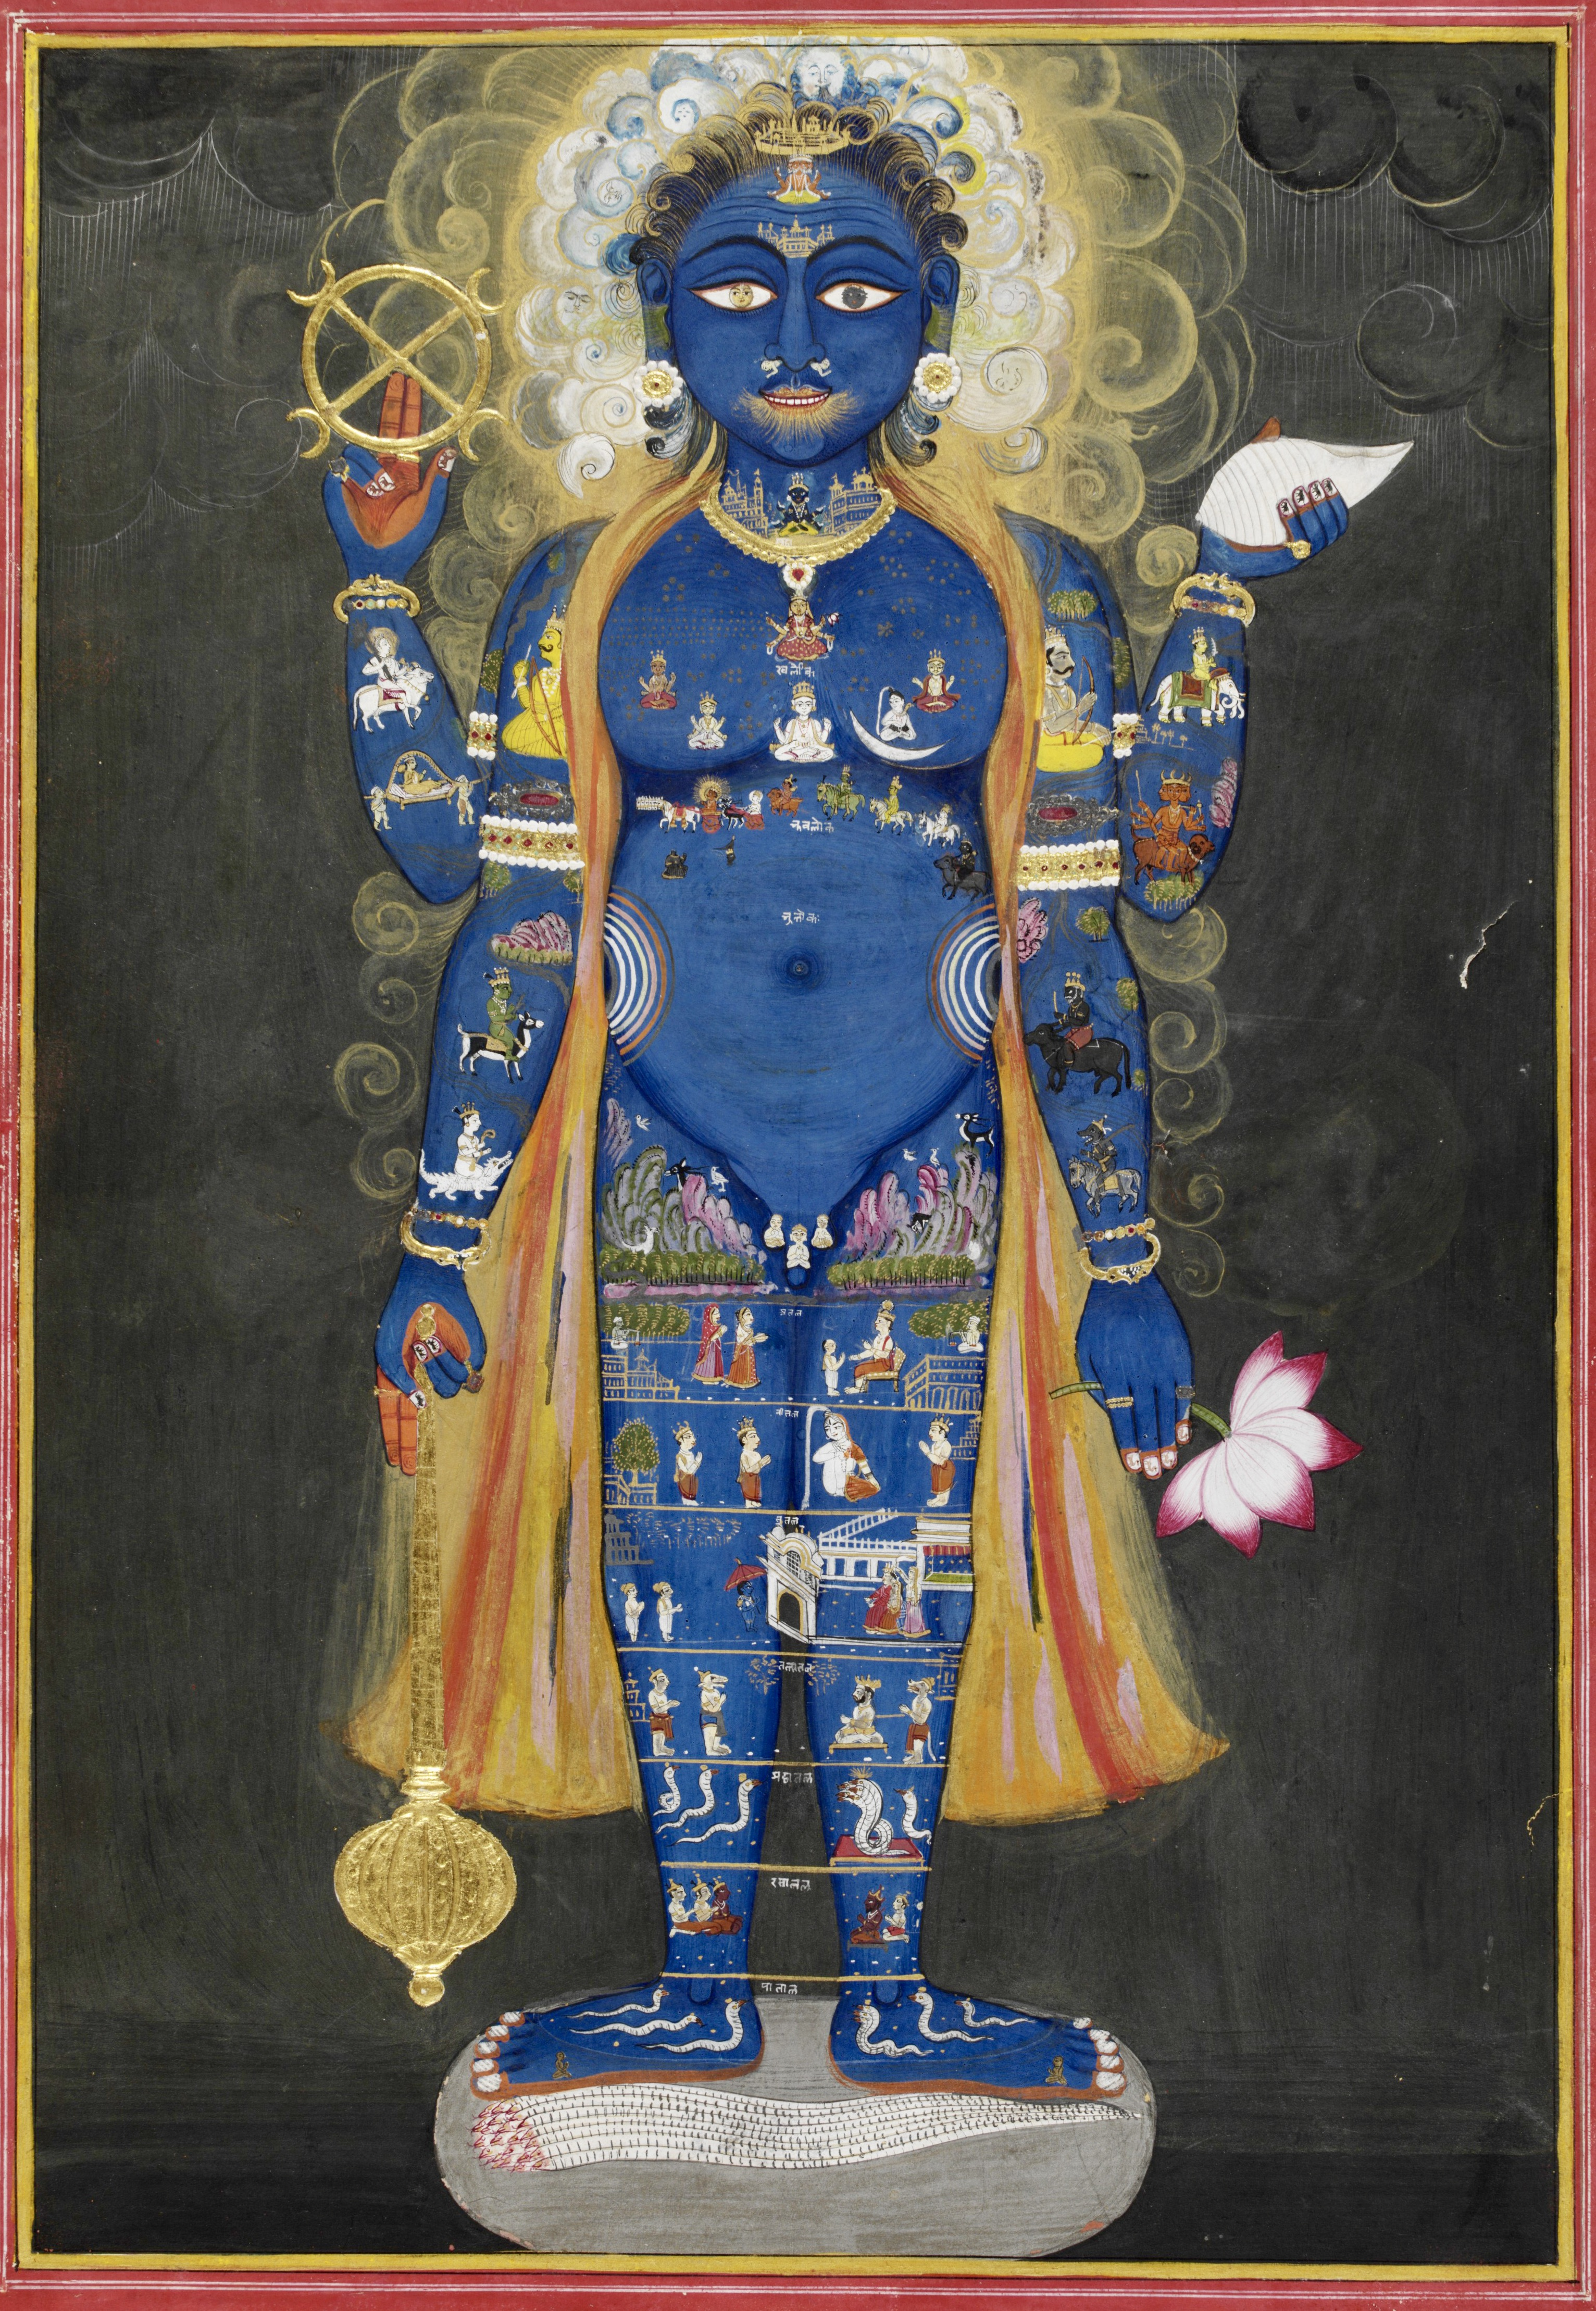
\includegraphics[width=1\textwidth]{pics/Vishnu_Vishvarupa_cropped.jpg}
	\caption[Viṣṇu Viśvarūpa]{Viṣṇu Viśvarūpa, India, Rajasthan, Jaipur, ca. 1800–1820, Opaque watercolor and gold on paper, 38.5 × 28 cm, Victoria and Albert Museum, London, Given by Mrs. Gerald Clark.}
	\label{fig:vishnu}
      \end{figure}
    
\clearpage
  \begin{figure}[ht]
	\centering
  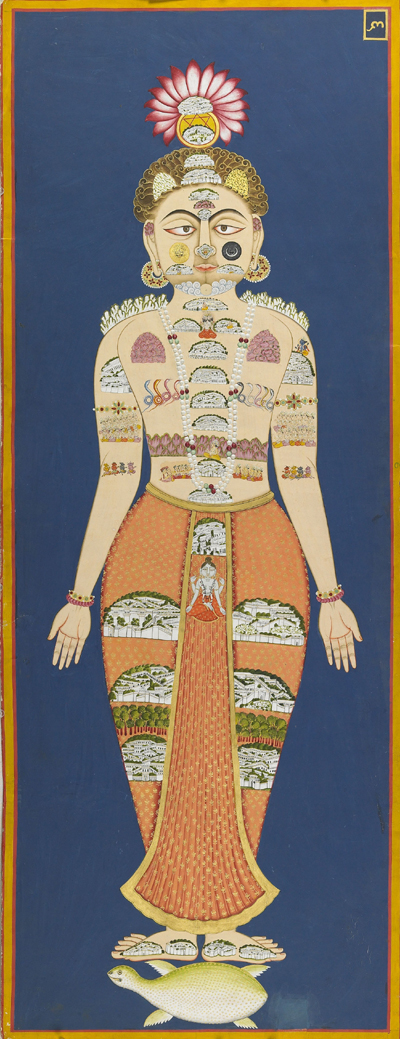
\includegraphics[width=0.5\textwidth]{pics/The_Equivalence_of_Self_and_Universe_(detail),_folio_6_from_the_Siddha_Siddhanta_Paddhati,_(Bulaki),_1824_(Samvat_1881);_122_x_46_cm._Mehrangarh_Museum_Trust..jpg}
	\caption[The Equivalence of the Self and the Universe]{The Equivalence of the Self and the Universe (detail), folio 6 from the \textit{Siddhasiddhāntapaddhati} (Bulaki), India, Rajasthan, Jodhpur, 1824 (Samvat 1881), 122 x 46 cm, RJS 2378, Mehragarh Museum Trust.}
	\label{fig:brahmanda}
      \end{figure}
      % \end{landscape}
\cleardoublepage

\backmatter
\chapter{Appendix}
\cleardoublepage
\section{The new digital tools used for the preparation of this dissertation}

The contemporary discourse, mainly triggered by last year's AI revolution, has led to significant debates within the university context. There are no universally accepted and definitive rules, especially concerning the drafting of academic papers or written exams. However, it is already clear that AI and other new digital tools, similar to the printing press or the internet, will transform our daily lives and become indispensable in academia. Their advantages are too significant to be ignored. Historically, beneficial technology has almost always prevailed. Another factor seems equally clear: within the academic context, clearly defined rules must be adhered to, regulating the use of these new digital tools and artificial intelligence in scholarly work, particularly in the context of assessments. These rules are constantly refined, with many universities still in a dynamic negotiation process to establish them. After all, until about a year ago, few anticipated such rapid developments. It is a delicate balance between harnessing potential and justified restriction. One core aspect that is likely to become a standard in dealing with digital tools and artificial intelligence is transparency. Since this dissertation constitutes an assessment, I will comprehensively explain how I have utilized new digital tools and artificial intelligence in this work.

The decision to write this dissertation in English was made when applying for admission to the doctoral program. As a non-native speaker, this was a challenge despite my relatively strong command of English, especially when trying to articulate complex matters usually expressed in my native language with precise English. To improve my English formulations, I used Grammarly and DeepL. Sometimes, it was easier for me to draft a complex thought in German, translate it into English and then have it corrected by DeepL and Grammarly, which I would then review and revise. Additionally, since I never learned French but had to understand the contents of several works by French Indologists written in French, I used DeepL to translate entire PDF files of these articles and books, allowing me to access the content of these relevant texts for my research.

The official start of this dissertation project was December 5, 2019. However, more intensive work on this dissertation began only with the start of the project funding through my employment in the "Light on Haṭha" project from March 15, 2021. It was not until late summer 2023 that I began using ChatGPT. Over time, I have used ChatGPT in the following ways to complete my dissertation:

\begin{itemize}
\item I occasionally used ChatGPT to optimize some of my English formulations.
\item By far, the most frequent application was to have my \textsc{Bib}\TeX{} entries written. I could easily copy the bibliographic information available online for the work I cited and have ChatGPT convert this information into the format of a \textsc{Bib}\TeX{} entry. These entries were checked, corrected if necessary, and adapted to my specific needs before being copied into my .bib file. This saved me a lot of time and effort.
\item The most astonishing application was the following. Theodor Aufrecht noted in an entry I found in the \textit{New Catalogus Catalogorum} that the \emph{Yogatattvabindu} by Sundaradeva was quoted in his \emph{Haṭhasaṅketacadrikā}. Although I had several digital manuscripts and an e-text of the \emph{Haṭhasaṅketacadrikā}, it was challenging to find an unspecified passage of my text in this very lengthy work, as it quickly became apparent that Sundaradeva had not cited the \emph{Yogatattvabindu} with reference. It was like searching for a needle in a haystack. Then, an idea struck me. I asked ChatGPT to write a Python script, which I called \textit{matchi}, to compare two .txt files: an e-text of the \emph{Yogatattvabindu} and an e-text of the \emph{Haṭhasaṅketacadrikā}. I had ChatGPT include variables to adjust the degree of similarity and the number of character sequences so a quote would be visible even if editorial changes or similar modifications were present. A few minutes later, using this program, I was able to identify all quotes from the \emph{Yogatattvabindu} in Sundaradeva's \emph{Haṭhasaṅketacadrikā}, saving me hours of searching.
\item For this work, about thirty verses from Sundardās' \emph{Sarvāṅgayogapradīpikā} were translated by me. These are written in Brajbhāṣā, a language I had no prior knowledge of before this dissertation. Through my Sanskrit training and two semesters of Hindi at the University of Heidelberg, I could only roughly understand the content of the verses. Thanks to a combination of Rupert Snell's article \citetitle{snell2016brajinbrief} (2016) and the help of ChatGPT, I was able to produce meaningful translations of the verses. A few weeks before submitting the dissertation, Dr. Felix Otter kindly agreed to review these translations. I was surprised that these translations contained hardly any errors.
\item It was evident to test ChatGPT's capability in translating Sanskrit. The results were surprisingly good, but the technology is still far from correctly contextualizing a passage, recognizing grammatical special cases, or capturing the ideal word choice in the target language. In other words, AI cannopt replace a well-trained Sanskritist. However, translations already achieve a degree of accuracy that makes them sometimes beneficial. Contemporary philological work involves searching through literary evidence in many typed transcriptions of thousands of Sanskrit texts shared among Indologists using grep (global regular expression search and print) or similar methods. To grasp the context of specific hits in these searches more quickly, I often fed larger chunks of the search hit context into ChatGPT and could thus find exactly the passages I was looking for much faster, which I then examined more closely if necessary.
\end{itemize}
\cleardoublepage

\chapter{Bibliography}
 \label{sec:bibli}
\clearpage
\newpage 
\thispagestyle{empty}
%\quad  \addtocounter{page}{-1}

\newrefcontext[sorting=tixel]
\printbibliography[heading=subbibintoc, title=Primary Sources, keyword=primary]

\newrefcontext[sorting=nyt]
\printbibliography[heading=subbibintoc, title=Secondary Literature, keyword=seclit]

\printbibliography[heading=subbibintoc, title=Catalogues, keyword=catalogues]

\printbibliography[heading=subbibintoc, title=Online Sources, keyword=onlinesource]

\end{document}


